\section{Optymalizacja parametrów regulatorów PID i DMC}
\label{projekt:zad5}


Dla zaproponowanej trajektorii zmian sygnału zadanego dobrano nastawy
regulatora PID w wyniku optymalizacji wskaźnika jakości regulacji E.
Optymalizacji dokonano za pomocą wbudowanej funkcji MATLABa $fmincon$.

\subsection{Optymalizacja PID}

\subsubsection{Konfiguracja regulatorów PID niesterująca wejściem $u_{1}$}

\begin{table}[H]
    \centering
    \begin{tabular}{|l|c|c|c|}
    \hline
         & Kr  & Ti  & Td  \\ \hline
    PID1 & --- & --- & --- \\ \hline
    PID2 & 2.438 & 3.2542 & 0.0 \\ \hline
    PID3 & 8.8647 & 0.2623 & 0.0 \\ \hline
    PID4 & 3.1042 & 16.8144 & 1.0262 \\ \hline
    \end{tabular}
    \caption[H]{Nastawy konfiguracji regulatorów bez PID1}
\end{table}

% Kr1=2.438 Td1=0 Ti1=3.2542 
% Kr2=8.8647 Td2=0 Ti2=0.2623 
% Kr3=3.1042 Td3=1.0262 Ti3=16.8144

\ifdefined\CompileFigures
\begin{figure}[H] 
    \centering
    % This file was created by matlab2tikz.
%
\definecolor{mycolor1}{rgb}{0.00000,0.44700,0.74100}%
%
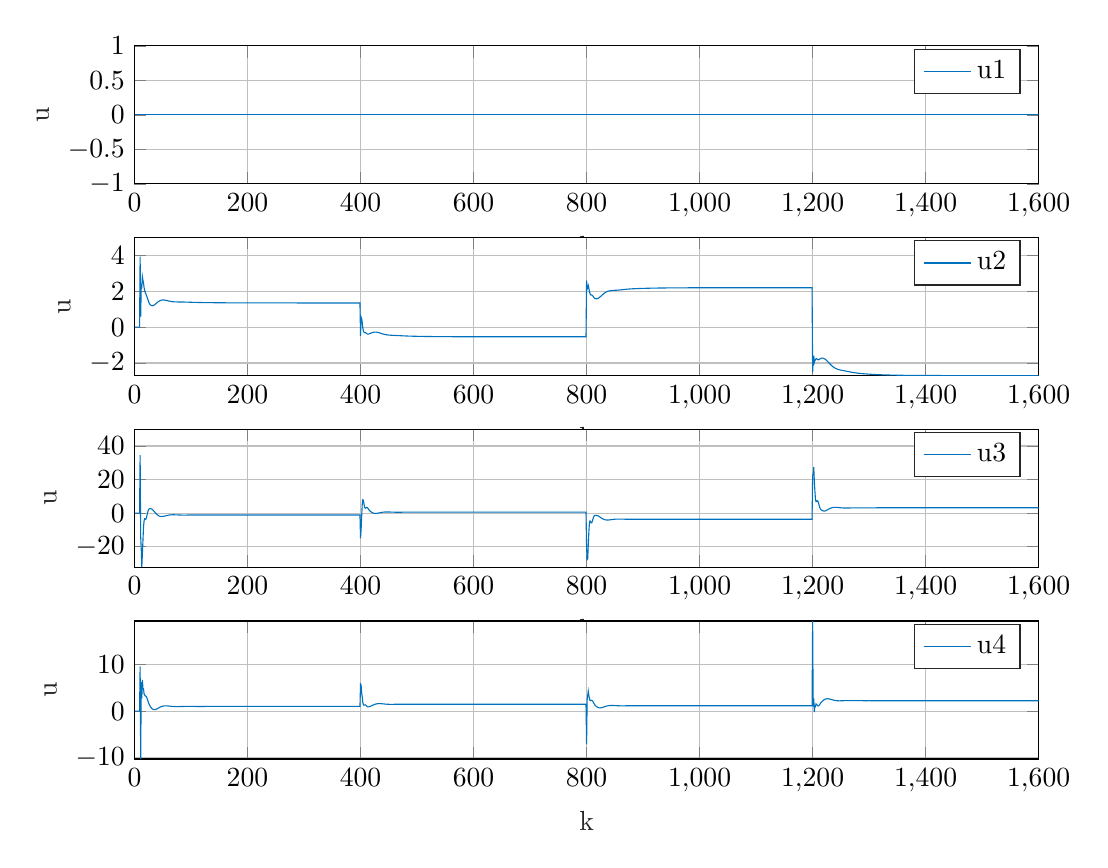
\begin{tikzpicture}

\begin{axis}[%
width=4.521in,
height=0.69in,
at={(0.758in,3.357in)},
scale only axis,
xmin=0,
xmax=1600,
xlabel style={font=\color{white!15!black}},
xlabel={k},
ymin=-1,
ymax=1,
ylabel style={font=\color{white!15!black}},
ylabel={u},
axis background/.style={fill=white},
xmajorgrids,
ymajorgrids,
legend style={legend cell align=left, align=left, draw=white!15!black}
]
\addplot [color=mycolor1]
  table[row sep=crcr]{%
1	0\\
2	0\\
3	0\\
4	0\\
5	0\\
6	0\\
7	0\\
8	0\\
9	0\\
10	0\\
11	0\\
12	0\\
13	0\\
14	0\\
15	0\\
16	0\\
17	0\\
18	0\\
19	0\\
20	0\\
21	0\\
22	0\\
23	0\\
24	0\\
25	0\\
26	0\\
27	0\\
28	0\\
29	0\\
30	0\\
31	0\\
32	0\\
33	0\\
34	0\\
35	0\\
36	0\\
37	0\\
38	0\\
39	0\\
40	0\\
41	0\\
42	0\\
43	0\\
44	0\\
45	0\\
46	0\\
47	0\\
48	0\\
49	0\\
50	0\\
51	0\\
52	0\\
53	0\\
54	0\\
55	0\\
56	0\\
57	0\\
58	0\\
59	0\\
60	0\\
61	0\\
62	0\\
63	0\\
64	0\\
65	0\\
66	0\\
67	0\\
68	0\\
69	0\\
70	0\\
71	0\\
72	0\\
73	0\\
74	0\\
75	0\\
76	0\\
77	0\\
78	0\\
79	0\\
80	0\\
81	0\\
82	0\\
83	0\\
84	0\\
85	0\\
86	0\\
87	0\\
88	0\\
89	0\\
90	0\\
91	0\\
92	0\\
93	0\\
94	0\\
95	0\\
96	0\\
97	0\\
98	0\\
99	0\\
100	0\\
101	0\\
102	0\\
103	0\\
104	0\\
105	0\\
106	0\\
107	0\\
108	0\\
109	0\\
110	0\\
111	0\\
112	0\\
113	0\\
114	0\\
115	0\\
116	0\\
117	0\\
118	0\\
119	0\\
120	0\\
121	0\\
122	0\\
123	0\\
124	0\\
125	0\\
126	0\\
127	0\\
128	0\\
129	0\\
130	0\\
131	0\\
132	0\\
133	0\\
134	0\\
135	0\\
136	0\\
137	0\\
138	0\\
139	0\\
140	0\\
141	0\\
142	0\\
143	0\\
144	0\\
145	0\\
146	0\\
147	0\\
148	0\\
149	0\\
150	0\\
151	0\\
152	0\\
153	0\\
154	0\\
155	0\\
156	0\\
157	0\\
158	0\\
159	0\\
160	0\\
161	0\\
162	0\\
163	0\\
164	0\\
165	0\\
166	0\\
167	0\\
168	0\\
169	0\\
170	0\\
171	0\\
172	0\\
173	0\\
174	0\\
175	0\\
176	0\\
177	0\\
178	0\\
179	0\\
180	0\\
181	0\\
182	0\\
183	0\\
184	0\\
185	0\\
186	0\\
187	0\\
188	0\\
189	0\\
190	0\\
191	0\\
192	0\\
193	0\\
194	0\\
195	0\\
196	0\\
197	0\\
198	0\\
199	0\\
200	0\\
201	0\\
202	0\\
203	0\\
204	0\\
205	0\\
206	0\\
207	0\\
208	0\\
209	0\\
210	0\\
211	0\\
212	0\\
213	0\\
214	0\\
215	0\\
216	0\\
217	0\\
218	0\\
219	0\\
220	0\\
221	0\\
222	0\\
223	0\\
224	0\\
225	0\\
226	0\\
227	0\\
228	0\\
229	0\\
230	0\\
231	0\\
232	0\\
233	0\\
234	0\\
235	0\\
236	0\\
237	0\\
238	0\\
239	0\\
240	0\\
241	0\\
242	0\\
243	0\\
244	0\\
245	0\\
246	0\\
247	0\\
248	0\\
249	0\\
250	0\\
251	0\\
252	0\\
253	0\\
254	0\\
255	0\\
256	0\\
257	0\\
258	0\\
259	0\\
260	0\\
261	0\\
262	0\\
263	0\\
264	0\\
265	0\\
266	0\\
267	0\\
268	0\\
269	0\\
270	0\\
271	0\\
272	0\\
273	0\\
274	0\\
275	0\\
276	0\\
277	0\\
278	0\\
279	0\\
280	0\\
281	0\\
282	0\\
283	0\\
284	0\\
285	0\\
286	0\\
287	0\\
288	0\\
289	0\\
290	0\\
291	0\\
292	0\\
293	0\\
294	0\\
295	0\\
296	0\\
297	0\\
298	0\\
299	0\\
300	0\\
301	0\\
302	0\\
303	0\\
304	0\\
305	0\\
306	0\\
307	0\\
308	0\\
309	0\\
310	0\\
311	0\\
312	0\\
313	0\\
314	0\\
315	0\\
316	0\\
317	0\\
318	0\\
319	0\\
320	0\\
321	0\\
322	0\\
323	0\\
324	0\\
325	0\\
326	0\\
327	0\\
328	0\\
329	0\\
330	0\\
331	0\\
332	0\\
333	0\\
334	0\\
335	0\\
336	0\\
337	0\\
338	0\\
339	0\\
340	0\\
341	0\\
342	0\\
343	0\\
344	0\\
345	0\\
346	0\\
347	0\\
348	0\\
349	0\\
350	0\\
351	0\\
352	0\\
353	0\\
354	0\\
355	0\\
356	0\\
357	0\\
358	0\\
359	0\\
360	0\\
361	0\\
362	0\\
363	0\\
364	0\\
365	0\\
366	0\\
367	0\\
368	0\\
369	0\\
370	0\\
371	0\\
372	0\\
373	0\\
374	0\\
375	0\\
376	0\\
377	0\\
378	0\\
379	0\\
380	0\\
381	0\\
382	0\\
383	0\\
384	0\\
385	0\\
386	0\\
387	0\\
388	0\\
389	0\\
390	0\\
391	0\\
392	0\\
393	0\\
394	0\\
395	0\\
396	0\\
397	0\\
398	0\\
399	0\\
400	0\\
401	0\\
402	0\\
403	0\\
404	0\\
405	0\\
406	0\\
407	0\\
408	0\\
409	0\\
410	0\\
411	0\\
412	0\\
413	0\\
414	0\\
415	0\\
416	0\\
417	0\\
418	0\\
419	0\\
420	0\\
421	0\\
422	0\\
423	0\\
424	0\\
425	0\\
426	0\\
427	0\\
428	0\\
429	0\\
430	0\\
431	0\\
432	0\\
433	0\\
434	0\\
435	0\\
436	0\\
437	0\\
438	0\\
439	0\\
440	0\\
441	0\\
442	0\\
443	0\\
444	0\\
445	0\\
446	0\\
447	0\\
448	0\\
449	0\\
450	0\\
451	0\\
452	0\\
453	0\\
454	0\\
455	0\\
456	0\\
457	0\\
458	0\\
459	0\\
460	0\\
461	0\\
462	0\\
463	0\\
464	0\\
465	0\\
466	0\\
467	0\\
468	0\\
469	0\\
470	0\\
471	0\\
472	0\\
473	0\\
474	0\\
475	0\\
476	0\\
477	0\\
478	0\\
479	0\\
480	0\\
481	0\\
482	0\\
483	0\\
484	0\\
485	0\\
486	0\\
487	0\\
488	0\\
489	0\\
490	0\\
491	0\\
492	0\\
493	0\\
494	0\\
495	0\\
496	0\\
497	0\\
498	0\\
499	0\\
500	0\\
501	0\\
502	0\\
503	0\\
504	0\\
505	0\\
506	0\\
507	0\\
508	0\\
509	0\\
510	0\\
511	0\\
512	0\\
513	0\\
514	0\\
515	0\\
516	0\\
517	0\\
518	0\\
519	0\\
520	0\\
521	0\\
522	0\\
523	0\\
524	0\\
525	0\\
526	0\\
527	0\\
528	0\\
529	0\\
530	0\\
531	0\\
532	0\\
533	0\\
534	0\\
535	0\\
536	0\\
537	0\\
538	0\\
539	0\\
540	0\\
541	0\\
542	0\\
543	0\\
544	0\\
545	0\\
546	0\\
547	0\\
548	0\\
549	0\\
550	0\\
551	0\\
552	0\\
553	0\\
554	0\\
555	0\\
556	0\\
557	0\\
558	0\\
559	0\\
560	0\\
561	0\\
562	0\\
563	0\\
564	0\\
565	0\\
566	0\\
567	0\\
568	0\\
569	0\\
570	0\\
571	0\\
572	0\\
573	0\\
574	0\\
575	0\\
576	0\\
577	0\\
578	0\\
579	0\\
580	0\\
581	0\\
582	0\\
583	0\\
584	0\\
585	0\\
586	0\\
587	0\\
588	0\\
589	0\\
590	0\\
591	0\\
592	0\\
593	0\\
594	0\\
595	0\\
596	0\\
597	0\\
598	0\\
599	0\\
600	0\\
601	0\\
602	0\\
603	0\\
604	0\\
605	0\\
606	0\\
607	0\\
608	0\\
609	0\\
610	0\\
611	0\\
612	0\\
613	0\\
614	0\\
615	0\\
616	0\\
617	0\\
618	0\\
619	0\\
620	0\\
621	0\\
622	0\\
623	0\\
624	0\\
625	0\\
626	0\\
627	0\\
628	0\\
629	0\\
630	0\\
631	0\\
632	0\\
633	0\\
634	0\\
635	0\\
636	0\\
637	0\\
638	0\\
639	0\\
640	0\\
641	0\\
642	0\\
643	0\\
644	0\\
645	0\\
646	0\\
647	0\\
648	0\\
649	0\\
650	0\\
651	0\\
652	0\\
653	0\\
654	0\\
655	0\\
656	0\\
657	0\\
658	0\\
659	0\\
660	0\\
661	0\\
662	0\\
663	0\\
664	0\\
665	0\\
666	0\\
667	0\\
668	0\\
669	0\\
670	0\\
671	0\\
672	0\\
673	0\\
674	0\\
675	0\\
676	0\\
677	0\\
678	0\\
679	0\\
680	0\\
681	0\\
682	0\\
683	0\\
684	0\\
685	0\\
686	0\\
687	0\\
688	0\\
689	0\\
690	0\\
691	0\\
692	0\\
693	0\\
694	0\\
695	0\\
696	0\\
697	0\\
698	0\\
699	0\\
700	0\\
701	0\\
702	0\\
703	0\\
704	0\\
705	0\\
706	0\\
707	0\\
708	0\\
709	0\\
710	0\\
711	0\\
712	0\\
713	0\\
714	0\\
715	0\\
716	0\\
717	0\\
718	0\\
719	0\\
720	0\\
721	0\\
722	0\\
723	0\\
724	0\\
725	0\\
726	0\\
727	0\\
728	0\\
729	0\\
730	0\\
731	0\\
732	0\\
733	0\\
734	0\\
735	0\\
736	0\\
737	0\\
738	0\\
739	0\\
740	0\\
741	0\\
742	0\\
743	0\\
744	0\\
745	0\\
746	0\\
747	0\\
748	0\\
749	0\\
750	0\\
751	0\\
752	0\\
753	0\\
754	0\\
755	0\\
756	0\\
757	0\\
758	0\\
759	0\\
760	0\\
761	0\\
762	0\\
763	0\\
764	0\\
765	0\\
766	0\\
767	0\\
768	0\\
769	0\\
770	0\\
771	0\\
772	0\\
773	0\\
774	0\\
775	0\\
776	0\\
777	0\\
778	0\\
779	0\\
780	0\\
781	0\\
782	0\\
783	0\\
784	0\\
785	0\\
786	0\\
787	0\\
788	0\\
789	0\\
790	0\\
791	0\\
792	0\\
793	0\\
794	0\\
795	0\\
796	0\\
797	0\\
798	0\\
799	0\\
800	0\\
801	0\\
802	0\\
803	0\\
804	0\\
805	0\\
806	0\\
807	0\\
808	0\\
809	0\\
810	0\\
811	0\\
812	0\\
813	0\\
814	0\\
815	0\\
816	0\\
817	0\\
818	0\\
819	0\\
820	0\\
821	0\\
822	0\\
823	0\\
824	0\\
825	0\\
826	0\\
827	0\\
828	0\\
829	0\\
830	0\\
831	0\\
832	0\\
833	0\\
834	0\\
835	0\\
836	0\\
837	0\\
838	0\\
839	0\\
840	0\\
841	0\\
842	0\\
843	0\\
844	0\\
845	0\\
846	0\\
847	0\\
848	0\\
849	0\\
850	0\\
851	0\\
852	0\\
853	0\\
854	0\\
855	0\\
856	0\\
857	0\\
858	0\\
859	0\\
860	0\\
861	0\\
862	0\\
863	0\\
864	0\\
865	0\\
866	0\\
867	0\\
868	0\\
869	0\\
870	0\\
871	0\\
872	0\\
873	0\\
874	0\\
875	0\\
876	0\\
877	0\\
878	0\\
879	0\\
880	0\\
881	0\\
882	0\\
883	0\\
884	0\\
885	0\\
886	0\\
887	0\\
888	0\\
889	0\\
890	0\\
891	0\\
892	0\\
893	0\\
894	0\\
895	0\\
896	0\\
897	0\\
898	0\\
899	0\\
900	0\\
901	0\\
902	0\\
903	0\\
904	0\\
905	0\\
906	0\\
907	0\\
908	0\\
909	0\\
910	0\\
911	0\\
912	0\\
913	0\\
914	0\\
915	0\\
916	0\\
917	0\\
918	0\\
919	0\\
920	0\\
921	0\\
922	0\\
923	0\\
924	0\\
925	0\\
926	0\\
927	0\\
928	0\\
929	0\\
930	0\\
931	0\\
932	0\\
933	0\\
934	0\\
935	0\\
936	0\\
937	0\\
938	0\\
939	0\\
940	0\\
941	0\\
942	0\\
943	0\\
944	0\\
945	0\\
946	0\\
947	0\\
948	0\\
949	0\\
950	0\\
951	0\\
952	0\\
953	0\\
954	0\\
955	0\\
956	0\\
957	0\\
958	0\\
959	0\\
960	0\\
961	0\\
962	0\\
963	0\\
964	0\\
965	0\\
966	0\\
967	0\\
968	0\\
969	0\\
970	0\\
971	0\\
972	0\\
973	0\\
974	0\\
975	0\\
976	0\\
977	0\\
978	0\\
979	0\\
980	0\\
981	0\\
982	0\\
983	0\\
984	0\\
985	0\\
986	0\\
987	0\\
988	0\\
989	0\\
990	0\\
991	0\\
992	0\\
993	0\\
994	0\\
995	0\\
996	0\\
997	0\\
998	0\\
999	0\\
1000	0\\
1001	0\\
1002	0\\
1003	0\\
1004	0\\
1005	0\\
1006	0\\
1007	0\\
1008	0\\
1009	0\\
1010	0\\
1011	0\\
1012	0\\
1013	0\\
1014	0\\
1015	0\\
1016	0\\
1017	0\\
1018	0\\
1019	0\\
1020	0\\
1021	0\\
1022	0\\
1023	0\\
1024	0\\
1025	0\\
1026	0\\
1027	0\\
1028	0\\
1029	0\\
1030	0\\
1031	0\\
1032	0\\
1033	0\\
1034	0\\
1035	0\\
1036	0\\
1037	0\\
1038	0\\
1039	0\\
1040	0\\
1041	0\\
1042	0\\
1043	0\\
1044	0\\
1045	0\\
1046	0\\
1047	0\\
1048	0\\
1049	0\\
1050	0\\
1051	0\\
1052	0\\
1053	0\\
1054	0\\
1055	0\\
1056	0\\
1057	0\\
1058	0\\
1059	0\\
1060	0\\
1061	0\\
1062	0\\
1063	0\\
1064	0\\
1065	0\\
1066	0\\
1067	0\\
1068	0\\
1069	0\\
1070	0\\
1071	0\\
1072	0\\
1073	0\\
1074	0\\
1075	0\\
1076	0\\
1077	0\\
1078	0\\
1079	0\\
1080	0\\
1081	0\\
1082	0\\
1083	0\\
1084	0\\
1085	0\\
1086	0\\
1087	0\\
1088	0\\
1089	0\\
1090	0\\
1091	0\\
1092	0\\
1093	0\\
1094	0\\
1095	0\\
1096	0\\
1097	0\\
1098	0\\
1099	0\\
1100	0\\
1101	0\\
1102	0\\
1103	0\\
1104	0\\
1105	0\\
1106	0\\
1107	0\\
1108	0\\
1109	0\\
1110	0\\
1111	0\\
1112	0\\
1113	0\\
1114	0\\
1115	0\\
1116	0\\
1117	0\\
1118	0\\
1119	0\\
1120	0\\
1121	0\\
1122	0\\
1123	0\\
1124	0\\
1125	0\\
1126	0\\
1127	0\\
1128	0\\
1129	0\\
1130	0\\
1131	0\\
1132	0\\
1133	0\\
1134	0\\
1135	0\\
1136	0\\
1137	0\\
1138	0\\
1139	0\\
1140	0\\
1141	0\\
1142	0\\
1143	0\\
1144	0\\
1145	0\\
1146	0\\
1147	0\\
1148	0\\
1149	0\\
1150	0\\
1151	0\\
1152	0\\
1153	0\\
1154	0\\
1155	0\\
1156	0\\
1157	0\\
1158	0\\
1159	0\\
1160	0\\
1161	0\\
1162	0\\
1163	0\\
1164	0\\
1165	0\\
1166	0\\
1167	0\\
1168	0\\
1169	0\\
1170	0\\
1171	0\\
1172	0\\
1173	0\\
1174	0\\
1175	0\\
1176	0\\
1177	0\\
1178	0\\
1179	0\\
1180	0\\
1181	0\\
1182	0\\
1183	0\\
1184	0\\
1185	0\\
1186	0\\
1187	0\\
1188	0\\
1189	0\\
1190	0\\
1191	0\\
1192	0\\
1193	0\\
1194	0\\
1195	0\\
1196	0\\
1197	0\\
1198	0\\
1199	0\\
1200	0\\
1201	0\\
1202	0\\
1203	0\\
1204	0\\
1205	0\\
1206	0\\
1207	0\\
1208	0\\
1209	0\\
1210	0\\
1211	0\\
1212	0\\
1213	0\\
1214	0\\
1215	0\\
1216	0\\
1217	0\\
1218	0\\
1219	0\\
1220	0\\
1221	0\\
1222	0\\
1223	0\\
1224	0\\
1225	0\\
1226	0\\
1227	0\\
1228	0\\
1229	0\\
1230	0\\
1231	0\\
1232	0\\
1233	0\\
1234	0\\
1235	0\\
1236	0\\
1237	0\\
1238	0\\
1239	0\\
1240	0\\
1241	0\\
1242	0\\
1243	0\\
1244	0\\
1245	0\\
1246	0\\
1247	0\\
1248	0\\
1249	0\\
1250	0\\
1251	0\\
1252	0\\
1253	0\\
1254	0\\
1255	0\\
1256	0\\
1257	0\\
1258	0\\
1259	0\\
1260	0\\
1261	0\\
1262	0\\
1263	0\\
1264	0\\
1265	0\\
1266	0\\
1267	0\\
1268	0\\
1269	0\\
1270	0\\
1271	0\\
1272	0\\
1273	0\\
1274	0\\
1275	0\\
1276	0\\
1277	0\\
1278	0\\
1279	0\\
1280	0\\
1281	0\\
1282	0\\
1283	0\\
1284	0\\
1285	0\\
1286	0\\
1287	0\\
1288	0\\
1289	0\\
1290	0\\
1291	0\\
1292	0\\
1293	0\\
1294	0\\
1295	0\\
1296	0\\
1297	0\\
1298	0\\
1299	0\\
1300	0\\
1301	0\\
1302	0\\
1303	0\\
1304	0\\
1305	0\\
1306	0\\
1307	0\\
1308	0\\
1309	0\\
1310	0\\
1311	0\\
1312	0\\
1313	0\\
1314	0\\
1315	0\\
1316	0\\
1317	0\\
1318	0\\
1319	0\\
1320	0\\
1321	0\\
1322	0\\
1323	0\\
1324	0\\
1325	0\\
1326	0\\
1327	0\\
1328	0\\
1329	0\\
1330	0\\
1331	0\\
1332	0\\
1333	0\\
1334	0\\
1335	0\\
1336	0\\
1337	0\\
1338	0\\
1339	0\\
1340	0\\
1341	0\\
1342	0\\
1343	0\\
1344	0\\
1345	0\\
1346	0\\
1347	0\\
1348	0\\
1349	0\\
1350	0\\
1351	0\\
1352	0\\
1353	0\\
1354	0\\
1355	0\\
1356	0\\
1357	0\\
1358	0\\
1359	0\\
1360	0\\
1361	0\\
1362	0\\
1363	0\\
1364	0\\
1365	0\\
1366	0\\
1367	0\\
1368	0\\
1369	0\\
1370	0\\
1371	0\\
1372	0\\
1373	0\\
1374	0\\
1375	0\\
1376	0\\
1377	0\\
1378	0\\
1379	0\\
1380	0\\
1381	0\\
1382	0\\
1383	0\\
1384	0\\
1385	0\\
1386	0\\
1387	0\\
1388	0\\
1389	0\\
1390	0\\
1391	0\\
1392	0\\
1393	0\\
1394	0\\
1395	0\\
1396	0\\
1397	0\\
1398	0\\
1399	0\\
1400	0\\
1401	0\\
1402	0\\
1403	0\\
1404	0\\
1405	0\\
1406	0\\
1407	0\\
1408	0\\
1409	0\\
1410	0\\
1411	0\\
1412	0\\
1413	0\\
1414	0\\
1415	0\\
1416	0\\
1417	0\\
1418	0\\
1419	0\\
1420	0\\
1421	0\\
1422	0\\
1423	0\\
1424	0\\
1425	0\\
1426	0\\
1427	0\\
1428	0\\
1429	0\\
1430	0\\
1431	0\\
1432	0\\
1433	0\\
1434	0\\
1435	0\\
1436	0\\
1437	0\\
1438	0\\
1439	0\\
1440	0\\
1441	0\\
1442	0\\
1443	0\\
1444	0\\
1445	0\\
1446	0\\
1447	0\\
1448	0\\
1449	0\\
1450	0\\
1451	0\\
1452	0\\
1453	0\\
1454	0\\
1455	0\\
1456	0\\
1457	0\\
1458	0\\
1459	0\\
1460	0\\
1461	0\\
1462	0\\
1463	0\\
1464	0\\
1465	0\\
1466	0\\
1467	0\\
1468	0\\
1469	0\\
1470	0\\
1471	0\\
1472	0\\
1473	0\\
1474	0\\
1475	0\\
1476	0\\
1477	0\\
1478	0\\
1479	0\\
1480	0\\
1481	0\\
1482	0\\
1483	0\\
1484	0\\
1485	0\\
1486	0\\
1487	0\\
1488	0\\
1489	0\\
1490	0\\
1491	0\\
1492	0\\
1493	0\\
1494	0\\
1495	0\\
1496	0\\
1497	0\\
1498	0\\
1499	0\\
1500	0\\
1501	0\\
1502	0\\
1503	0\\
1504	0\\
1505	0\\
1506	0\\
1507	0\\
1508	0\\
1509	0\\
1510	0\\
1511	0\\
1512	0\\
1513	0\\
1514	0\\
1515	0\\
1516	0\\
1517	0\\
1518	0\\
1519	0\\
1520	0\\
1521	0\\
1522	0\\
1523	0\\
1524	0\\
1525	0\\
1526	0\\
1527	0\\
1528	0\\
1529	0\\
1530	0\\
1531	0\\
1532	0\\
1533	0\\
1534	0\\
1535	0\\
1536	0\\
1537	0\\
1538	0\\
1539	0\\
1540	0\\
1541	0\\
1542	0\\
1543	0\\
1544	0\\
1545	0\\
1546	0\\
1547	0\\
1548	0\\
1549	0\\
1550	0\\
1551	0\\
1552	0\\
1553	0\\
1554	0\\
1555	0\\
1556	0\\
1557	0\\
1558	0\\
1559	0\\
1560	0\\
1561	0\\
1562	0\\
1563	0\\
1564	0\\
1565	0\\
1566	0\\
1567	0\\
1568	0\\
1569	0\\
1570	0\\
1571	0\\
1572	0\\
1573	0\\
1574	0\\
1575	0\\
1576	0\\
1577	0\\
1578	0\\
1579	0\\
1580	0\\
1581	0\\
1582	0\\
1583	0\\
1584	0\\
1585	0\\
1586	0\\
1587	0\\
1588	0\\
1589	0\\
1590	0\\
1591	0\\
1592	0\\
1593	0\\
1594	0\\
1595	0\\
1596	0\\
1597	0\\
1598	0\\
1599	0\\
1600	0\\
};
\addlegendentry{u1}

\end{axis}

\begin{axis}[%
width=4.521in,
height=0.69in,
at={(0.758in,2.398in)},
scale only axis,
xmin=0,
xmax=1600,
xlabel style={font=\color{white!15!black}},
xlabel={k},
ymin=-2.7027,
ymax=5,
ylabel style={font=\color{white!15!black}},
ylabel={u},
axis background/.style={fill=white},
xmajorgrids,
ymajorgrids,
legend style={legend cell align=left, align=left, draw=white!15!black}
]
\addplot [color=mycolor1]
  table[row sep=crcr]{%
1	0\\
2	0\\
3	0\\
4	0\\
5	0\\
6	0\\
7	0\\
8	0\\
9	0\\
10	3.9379\\
11	0.59085\\
12	2.3292\\
13	2.2732\\
14	2.8157\\
15	2.6148\\
16	2.4733\\
17	2.2085\\
18	2.0543\\
19	1.9388\\
20	1.8702\\
21	1.7969\\
22	1.7119\\
23	1.6123\\
24	1.5118\\
25	1.421\\
26	1.3474\\
27	1.2919\\
28	1.2522\\
29	1.2251\\
30	1.2079\\
31	1.1994\\
32	1.199\\
33	1.2061\\
34	1.22\\
35	1.2394\\
36	1.2628\\
37	1.2888\\
38	1.3162\\
39	1.3439\\
40	1.371\\
41	1.3969\\
42	1.421\\
43	1.4428\\
44	1.4621\\
45	1.4786\\
46	1.4921\\
47	1.5027\\
48	1.5105\\
49	1.5156\\
50	1.5181\\
51	1.5185\\
52	1.5169\\
53	1.5135\\
54	1.5088\\
55	1.503\\
56	1.4964\\
57	1.4892\\
58	1.4816\\
59	1.474\\
60	1.4664\\
61	1.4591\\
62	1.4521\\
63	1.4456\\
64	1.4396\\
65	1.4342\\
66	1.4294\\
67	1.4252\\
68	1.4215\\
69	1.4184\\
70	1.4159\\
71	1.4138\\
72	1.4121\\
73	1.4108\\
74	1.4099\\
75	1.4091\\
76	1.4086\\
77	1.4082\\
78	1.4078\\
79	1.4076\\
80	1.4073\\
81	1.4071\\
82	1.4068\\
83	1.4064\\
84	1.406\\
85	1.4055\\
86	1.4049\\
87	1.4042\\
88	1.4034\\
89	1.4025\\
90	1.4016\\
91	1.4006\\
92	1.3995\\
93	1.3984\\
94	1.3973\\
95	1.3962\\
96	1.395\\
97	1.3938\\
98	1.3927\\
99	1.3915\\
100	1.3904\\
101	1.3893\\
102	1.3883\\
103	1.3872\\
104	1.3863\\
105	1.3853\\
106	1.3844\\
107	1.3836\\
108	1.3827\\
109	1.382\\
110	1.3812\\
111	1.3805\\
112	1.3798\\
113	1.3792\\
114	1.3786\\
115	1.378\\
116	1.3774\\
117	1.3768\\
118	1.3763\\
119	1.3758\\
120	1.3752\\
121	1.3747\\
122	1.3743\\
123	1.3738\\
124	1.3733\\
125	1.3728\\
126	1.3724\\
127	1.3719\\
128	1.3715\\
129	1.371\\
130	1.3706\\
131	1.3702\\
132	1.3697\\
133	1.3693\\
134	1.3689\\
135	1.3685\\
136	1.3681\\
137	1.3677\\
138	1.3674\\
139	1.367\\
140	1.3666\\
141	1.3663\\
142	1.366\\
143	1.3656\\
144	1.3653\\
145	1.365\\
146	1.3647\\
147	1.3644\\
148	1.3641\\
149	1.3638\\
150	1.3635\\
151	1.3633\\
152	1.363\\
153	1.3627\\
154	1.3625\\
155	1.3623\\
156	1.362\\
157	1.3618\\
158	1.3616\\
159	1.3614\\
160	1.3611\\
161	1.3609\\
162	1.3607\\
163	1.3605\\
164	1.3603\\
165	1.3602\\
166	1.36\\
167	1.3598\\
168	1.3596\\
169	1.3594\\
170	1.3593\\
171	1.3591\\
172	1.3589\\
173	1.3588\\
174	1.3586\\
175	1.3585\\
176	1.3583\\
177	1.3582\\
178	1.3581\\
179	1.3579\\
180	1.3578\\
181	1.3577\\
182	1.3575\\
183	1.3574\\
184	1.3573\\
185	1.3572\\
186	1.3571\\
187	1.357\\
188	1.3568\\
189	1.3567\\
190	1.3566\\
191	1.3565\\
192	1.3564\\
193	1.3563\\
194	1.3562\\
195	1.3562\\
196	1.3561\\
197	1.356\\
198	1.3559\\
199	1.3558\\
200	1.3557\\
201	1.3556\\
202	1.3556\\
203	1.3555\\
204	1.3554\\
205	1.3554\\
206	1.3553\\
207	1.3552\\
208	1.3551\\
209	1.3551\\
210	1.355\\
211	1.355\\
212	1.3549\\
213	1.3548\\
214	1.3548\\
215	1.3547\\
216	1.3547\\
217	1.3546\\
218	1.3546\\
219	1.3545\\
220	1.3545\\
221	1.3544\\
222	1.3544\\
223	1.3543\\
224	1.3543\\
225	1.3542\\
226	1.3542\\
227	1.3541\\
228	1.3541\\
229	1.3541\\
230	1.354\\
231	1.354\\
232	1.354\\
233	1.3539\\
234	1.3539\\
235	1.3539\\
236	1.3538\\
237	1.3538\\
238	1.3538\\
239	1.3537\\
240	1.3537\\
241	1.3537\\
242	1.3536\\
243	1.3536\\
244	1.3536\\
245	1.3536\\
246	1.3535\\
247	1.3535\\
248	1.3535\\
249	1.3535\\
250	1.3534\\
251	1.3534\\
252	1.3534\\
253	1.3534\\
254	1.3533\\
255	1.3533\\
256	1.3533\\
257	1.3533\\
258	1.3533\\
259	1.3532\\
260	1.3532\\
261	1.3532\\
262	1.3532\\
263	1.3532\\
264	1.3531\\
265	1.3531\\
266	1.3531\\
267	1.3531\\
268	1.3531\\
269	1.3531\\
270	1.3531\\
271	1.353\\
272	1.353\\
273	1.353\\
274	1.353\\
275	1.353\\
276	1.353\\
277	1.353\\
278	1.353\\
279	1.3529\\
280	1.3529\\
281	1.3529\\
282	1.3529\\
283	1.3529\\
284	1.3529\\
285	1.3529\\
286	1.3529\\
287	1.3529\\
288	1.3528\\
289	1.3528\\
290	1.3528\\
291	1.3528\\
292	1.3528\\
293	1.3528\\
294	1.3528\\
295	1.3528\\
296	1.3528\\
297	1.3528\\
298	1.3528\\
299	1.3528\\
300	1.3528\\
301	1.3527\\
302	1.3527\\
303	1.3527\\
304	1.3527\\
305	1.3527\\
306	1.3527\\
307	1.3527\\
308	1.3527\\
309	1.3527\\
310	1.3527\\
311	1.3527\\
312	1.3527\\
313	1.3527\\
314	1.3527\\
315	1.3527\\
316	1.3527\\
317	1.3527\\
318	1.3527\\
319	1.3527\\
320	1.3526\\
321	1.3526\\
322	1.3526\\
323	1.3526\\
324	1.3526\\
325	1.3526\\
326	1.3526\\
327	1.3526\\
328	1.3526\\
329	1.3526\\
330	1.3526\\
331	1.3526\\
332	1.3526\\
333	1.3526\\
334	1.3526\\
335	1.3526\\
336	1.3526\\
337	1.3526\\
338	1.3526\\
339	1.3526\\
340	1.3526\\
341	1.3526\\
342	1.3526\\
343	1.3526\\
344	1.3526\\
345	1.3526\\
346	1.3526\\
347	1.3526\\
348	1.3526\\
349	1.3526\\
350	1.3526\\
351	1.3526\\
352	1.3526\\
353	1.3526\\
354	1.3526\\
355	1.3525\\
356	1.3525\\
357	1.3525\\
358	1.3525\\
359	1.3525\\
360	1.3525\\
361	1.3525\\
362	1.3525\\
363	1.3525\\
364	1.3525\\
365	1.3525\\
366	1.3525\\
367	1.3525\\
368	1.3525\\
369	1.3525\\
370	1.3525\\
371	1.3525\\
372	1.3525\\
373	1.3525\\
374	1.3525\\
375	1.3525\\
376	1.3525\\
377	1.3525\\
378	1.3525\\
379	1.3525\\
380	1.3525\\
381	1.3525\\
382	1.3525\\
383	1.3525\\
384	1.3525\\
385	1.3525\\
386	1.3525\\
387	1.3525\\
388	1.3525\\
389	1.3525\\
390	1.3525\\
391	1.3525\\
392	1.3525\\
393	1.3525\\
394	1.3525\\
395	1.3525\\
396	1.3525\\
397	1.3525\\
398	1.3525\\
399	1.3525\\
400	-0.48521\\
401	0.5623\\
402	0.48152\\
403	0.25327\\
404	-0.027602\\
405	-0.19609\\
406	-0.27957\\
407	-0.29812\\
408	-0.30207\\
409	-0.31209\\
410	-0.33452\\
411	-0.36051\\
412	-0.38071\\
413	-0.38941\\
414	-0.38684\\
415	-0.37654\\
416	-0.36276\\
417	-0.34853\\
418	-0.33525\\
419	-0.3231\\
420	-0.31192\\
421	-0.30165\\
422	-0.29251\\
423	-0.28491\\
424	-0.27926\\
425	-0.27578\\
426	-0.27452\\
427	-0.27537\\
428	-0.27814\\
429	-0.2826\\
430	-0.28853\\
431	-0.29571\\
432	-0.30392\\
433	-0.31294\\
434	-0.32253\\
435	-0.33248\\
436	-0.34258\\
437	-0.35265\\
438	-0.36252\\
439	-0.37207\\
440	-0.38118\\
441	-0.38977\\
442	-0.39778\\
443	-0.40517\\
444	-0.41192\\
445	-0.41802\\
446	-0.42351\\
447	-0.42839\\
448	-0.4327\\
449	-0.4365\\
450	-0.43983\\
451	-0.44274\\
452	-0.44529\\
453	-0.44754\\
454	-0.44954\\
455	-0.45133\\
456	-0.45296\\
457	-0.45448\\
458	-0.45592\\
459	-0.45732\\
460	-0.4587\\
461	-0.46007\\
462	-0.46147\\
463	-0.46289\\
464	-0.46435\\
465	-0.46585\\
466	-0.46739\\
467	-0.46896\\
468	-0.47058\\
469	-0.47222\\
470	-0.47388\\
471	-0.47555\\
472	-0.47722\\
473	-0.4789\\
474	-0.48055\\
475	-0.48219\\
476	-0.4838\\
477	-0.48538\\
478	-0.48691\\
479	-0.4884\\
480	-0.48985\\
481	-0.49124\\
482	-0.49258\\
483	-0.49387\\
484	-0.4951\\
485	-0.49629\\
486	-0.49742\\
487	-0.49851\\
488	-0.49954\\
489	-0.50054\\
490	-0.50149\\
491	-0.5024\\
492	-0.50328\\
493	-0.50413\\
494	-0.50494\\
495	-0.50573\\
496	-0.50649\\
497	-0.50723\\
498	-0.50795\\
499	-0.50865\\
500	-0.50933\\
501	-0.51\\
502	-0.51065\\
503	-0.51128\\
504	-0.5119\\
505	-0.51251\\
506	-0.51311\\
507	-0.51369\\
508	-0.51426\\
509	-0.51482\\
510	-0.51536\\
511	-0.5159\\
512	-0.51642\\
513	-0.51693\\
514	-0.51743\\
515	-0.51792\\
516	-0.51839\\
517	-0.51885\\
518	-0.5193\\
519	-0.51974\\
520	-0.52017\\
521	-0.52058\\
522	-0.52099\\
523	-0.52138\\
524	-0.52176\\
525	-0.52214\\
526	-0.5225\\
527	-0.52285\\
528	-0.52319\\
529	-0.52352\\
530	-0.52384\\
531	-0.52416\\
532	-0.52446\\
533	-0.52476\\
534	-0.52505\\
535	-0.52533\\
536	-0.52561\\
537	-0.52587\\
538	-0.52613\\
539	-0.52639\\
540	-0.52664\\
541	-0.52688\\
542	-0.52711\\
543	-0.52734\\
544	-0.52756\\
545	-0.52778\\
546	-0.528\\
547	-0.5282\\
548	-0.52841\\
549	-0.5286\\
550	-0.5288\\
551	-0.52898\\
552	-0.52917\\
553	-0.52934\\
554	-0.52952\\
555	-0.52969\\
556	-0.52985\\
557	-0.53002\\
558	-0.53017\\
559	-0.53033\\
560	-0.53048\\
561	-0.53062\\
562	-0.53076\\
563	-0.5309\\
564	-0.53104\\
565	-0.53117\\
566	-0.5313\\
567	-0.53142\\
568	-0.53154\\
569	-0.53166\\
570	-0.53178\\
571	-0.53189\\
572	-0.532\\
573	-0.53211\\
574	-0.53221\\
575	-0.53232\\
576	-0.53242\\
577	-0.53251\\
578	-0.53261\\
579	-0.5327\\
580	-0.53279\\
581	-0.53288\\
582	-0.53296\\
583	-0.53305\\
584	-0.53313\\
585	-0.53321\\
586	-0.53328\\
587	-0.53336\\
588	-0.53343\\
589	-0.53351\\
590	-0.53358\\
591	-0.53364\\
592	-0.53371\\
593	-0.53378\\
594	-0.53384\\
595	-0.5339\\
596	-0.53396\\
597	-0.53402\\
598	-0.53408\\
599	-0.53413\\
600	-0.53419\\
601	-0.53424\\
602	-0.53429\\
603	-0.53434\\
604	-0.53439\\
605	-0.53444\\
606	-0.53449\\
607	-0.53453\\
608	-0.53458\\
609	-0.53462\\
610	-0.53466\\
611	-0.53471\\
612	-0.53475\\
613	-0.53479\\
614	-0.53482\\
615	-0.53486\\
616	-0.5349\\
617	-0.53493\\
618	-0.53497\\
619	-0.535\\
620	-0.53504\\
621	-0.53507\\
622	-0.5351\\
623	-0.53513\\
624	-0.53516\\
625	-0.53519\\
626	-0.53522\\
627	-0.53525\\
628	-0.53527\\
629	-0.5353\\
630	-0.53533\\
631	-0.53535\\
632	-0.53538\\
633	-0.5354\\
634	-0.53542\\
635	-0.53545\\
636	-0.53547\\
637	-0.53549\\
638	-0.53551\\
639	-0.53553\\
640	-0.53555\\
641	-0.53557\\
642	-0.53559\\
643	-0.53561\\
644	-0.53563\\
645	-0.53565\\
646	-0.53566\\
647	-0.53568\\
648	-0.5357\\
649	-0.53571\\
650	-0.53573\\
651	-0.53575\\
652	-0.53576\\
653	-0.53577\\
654	-0.53579\\
655	-0.5358\\
656	-0.53582\\
657	-0.53583\\
658	-0.53584\\
659	-0.53586\\
660	-0.53587\\
661	-0.53588\\
662	-0.53589\\
663	-0.5359\\
664	-0.53591\\
665	-0.53592\\
666	-0.53594\\
667	-0.53595\\
668	-0.53596\\
669	-0.53597\\
670	-0.53598\\
671	-0.53598\\
672	-0.53599\\
673	-0.536\\
674	-0.53601\\
675	-0.53602\\
676	-0.53603\\
677	-0.53604\\
678	-0.53604\\
679	-0.53605\\
680	-0.53606\\
681	-0.53607\\
682	-0.53607\\
683	-0.53608\\
684	-0.53609\\
685	-0.53609\\
686	-0.5361\\
687	-0.53611\\
688	-0.53611\\
689	-0.53612\\
690	-0.53613\\
691	-0.53613\\
692	-0.53614\\
693	-0.53614\\
694	-0.53615\\
695	-0.53615\\
696	-0.53616\\
697	-0.53616\\
698	-0.53617\\
699	-0.53617\\
700	-0.53618\\
701	-0.53618\\
702	-0.53619\\
703	-0.53619\\
704	-0.53619\\
705	-0.5362\\
706	-0.5362\\
707	-0.53621\\
708	-0.53621\\
709	-0.53621\\
710	-0.53622\\
711	-0.53622\\
712	-0.53622\\
713	-0.53623\\
714	-0.53623\\
715	-0.53623\\
716	-0.53624\\
717	-0.53624\\
718	-0.53624\\
719	-0.53624\\
720	-0.53625\\
721	-0.53625\\
722	-0.53625\\
723	-0.53626\\
724	-0.53626\\
725	-0.53626\\
726	-0.53626\\
727	-0.53627\\
728	-0.53627\\
729	-0.53627\\
730	-0.53627\\
731	-0.53627\\
732	-0.53628\\
733	-0.53628\\
734	-0.53628\\
735	-0.53628\\
736	-0.53628\\
737	-0.53629\\
738	-0.53629\\
739	-0.53629\\
740	-0.53629\\
741	-0.53629\\
742	-0.53629\\
743	-0.5363\\
744	-0.5363\\
745	-0.5363\\
746	-0.5363\\
747	-0.5363\\
748	-0.5363\\
749	-0.5363\\
750	-0.53631\\
751	-0.53631\\
752	-0.53631\\
753	-0.53631\\
754	-0.53631\\
755	-0.53631\\
756	-0.53631\\
757	-0.53631\\
758	-0.53632\\
759	-0.53632\\
760	-0.53632\\
761	-0.53632\\
762	-0.53632\\
763	-0.53632\\
764	-0.53632\\
765	-0.53632\\
766	-0.53632\\
767	-0.53632\\
768	-0.53633\\
769	-0.53633\\
770	-0.53633\\
771	-0.53633\\
772	-0.53633\\
773	-0.53633\\
774	-0.53633\\
775	-0.53633\\
776	-0.53633\\
777	-0.53633\\
778	-0.53633\\
779	-0.53633\\
780	-0.53633\\
781	-0.53633\\
782	-0.53634\\
783	-0.53634\\
784	-0.53634\\
785	-0.53634\\
786	-0.53634\\
787	-0.53634\\
788	-0.53634\\
789	-0.53634\\
790	-0.53634\\
791	-0.53634\\
792	-0.53634\\
793	-0.53634\\
794	-0.53634\\
795	-0.53634\\
796	-0.53634\\
797	-0.53634\\
798	-0.53634\\
799	-0.53634\\
800	2.614\\
801	2.1308\\
802	2.1958\\
803	2.3239\\
804	2.1782\\
805	2.0192\\
806	1.8776\\
807	1.816\\
808	1.7979\\
809	1.7954\\
810	1.7794\\
811	1.7455\\
812	1.7001\\
813	1.6554\\
814	1.6199\\
815	1.5972\\
816	1.5858\\
817	1.5831\\
818	1.5863\\
819	1.594\\
820	1.606\\
821	1.6221\\
822	1.6423\\
823	1.6661\\
824	1.6925\\
825	1.7207\\
826	1.7497\\
827	1.7788\\
828	1.8074\\
829	1.8352\\
830	1.8618\\
831	1.8868\\
832	1.91\\
833	1.9313\\
834	1.9506\\
835	1.9678\\
836	1.9829\\
837	1.996\\
838	2.0073\\
839	2.0168\\
840	2.0248\\
841	2.0314\\
842	2.0368\\
843	2.0412\\
844	2.0448\\
845	2.0477\\
846	2.0501\\
847	2.0521\\
848	2.0539\\
849	2.0556\\
850	2.0572\\
851	2.059\\
852	2.0608\\
853	2.0628\\
854	2.065\\
855	2.0673\\
856	2.0699\\
857	2.0727\\
858	2.0756\\
859	2.0788\\
860	2.082\\
861	2.0854\\
862	2.0888\\
863	2.0923\\
864	2.0959\\
865	2.0994\\
866	2.1028\\
867	2.1063\\
868	2.1096\\
869	2.1128\\
870	2.116\\
871	2.119\\
872	2.1218\\
873	2.1246\\
874	2.1272\\
875	2.1296\\
876	2.132\\
877	2.1342\\
878	2.1362\\
879	2.1382\\
880	2.1401\\
881	2.1418\\
882	2.1435\\
883	2.1451\\
884	2.1466\\
885	2.148\\
886	2.1494\\
887	2.1508\\
888	2.152\\
889	2.1533\\
890	2.1545\\
891	2.1557\\
892	2.1569\\
893	2.158\\
894	2.1591\\
895	2.1602\\
896	2.1613\\
897	2.1624\\
898	2.1634\\
899	2.1644\\
900	2.1654\\
901	2.1664\\
902	2.1674\\
903	2.1683\\
904	2.1693\\
905	2.1702\\
906	2.171\\
907	2.1719\\
908	2.1727\\
909	2.1735\\
910	2.1743\\
911	2.1751\\
912	2.1758\\
913	2.1766\\
914	2.1773\\
915	2.1779\\
916	2.1786\\
917	2.1792\\
918	2.1798\\
919	2.1804\\
920	2.181\\
921	2.1816\\
922	2.1821\\
923	2.1827\\
924	2.1832\\
925	2.1837\\
926	2.1842\\
927	2.1846\\
928	2.1851\\
929	2.1855\\
930	2.186\\
931	2.1864\\
932	2.1868\\
933	2.1872\\
934	2.1876\\
935	2.188\\
936	2.1884\\
937	2.1887\\
938	2.1891\\
939	2.1894\\
940	2.1898\\
941	2.1901\\
942	2.1904\\
943	2.1907\\
944	2.1911\\
945	2.1914\\
946	2.1916\\
947	2.1919\\
948	2.1922\\
949	2.1925\\
950	2.1927\\
951	2.193\\
952	2.1932\\
953	2.1935\\
954	2.1937\\
955	2.1939\\
956	2.1942\\
957	2.1944\\
958	2.1946\\
959	2.1948\\
960	2.195\\
961	2.1952\\
962	2.1954\\
963	2.1956\\
964	2.1958\\
965	2.1959\\
966	2.1961\\
967	2.1963\\
968	2.1964\\
969	2.1966\\
970	2.1968\\
971	2.1969\\
972	2.1971\\
973	2.1972\\
974	2.1973\\
975	2.1975\\
976	2.1976\\
977	2.1977\\
978	2.1979\\
979	2.198\\
980	2.1981\\
981	2.1982\\
982	2.1983\\
983	2.1985\\
984	2.1986\\
985	2.1987\\
986	2.1988\\
987	2.1989\\
988	2.199\\
989	2.1991\\
990	2.1992\\
991	2.1993\\
992	2.1993\\
993	2.1994\\
994	2.1995\\
995	2.1996\\
996	2.1997\\
997	2.1998\\
998	2.1998\\
999	2.1999\\
1000	2.2\\
1001	2.2001\\
1002	2.2001\\
1003	2.2002\\
1004	2.2003\\
1005	2.2003\\
1006	2.2004\\
1007	2.2004\\
1008	2.2005\\
1009	2.2006\\
1010	2.2006\\
1011	2.2007\\
1012	2.2007\\
1013	2.2008\\
1014	2.2008\\
1015	2.2009\\
1016	2.2009\\
1017	2.201\\
1018	2.201\\
1019	2.2011\\
1020	2.2011\\
1021	2.2012\\
1022	2.2012\\
1023	2.2012\\
1024	2.2013\\
1025	2.2013\\
1026	2.2014\\
1027	2.2014\\
1028	2.2014\\
1029	2.2015\\
1030	2.2015\\
1031	2.2015\\
1032	2.2016\\
1033	2.2016\\
1034	2.2016\\
1035	2.2017\\
1036	2.2017\\
1037	2.2017\\
1038	2.2017\\
1039	2.2018\\
1040	2.2018\\
1041	2.2018\\
1042	2.2019\\
1043	2.2019\\
1044	2.2019\\
1045	2.2019\\
1046	2.2019\\
1047	2.202\\
1048	2.202\\
1049	2.202\\
1050	2.202\\
1051	2.2021\\
1052	2.2021\\
1053	2.2021\\
1054	2.2021\\
1055	2.2021\\
1056	2.2022\\
1057	2.2022\\
1058	2.2022\\
1059	2.2022\\
1060	2.2022\\
1061	2.2022\\
1062	2.2023\\
1063	2.2023\\
1064	2.2023\\
1065	2.2023\\
1066	2.2023\\
1067	2.2023\\
1068	2.2023\\
1069	2.2023\\
1070	2.2024\\
1071	2.2024\\
1072	2.2024\\
1073	2.2024\\
1074	2.2024\\
1075	2.2024\\
1076	2.2024\\
1077	2.2024\\
1078	2.2025\\
1079	2.2025\\
1080	2.2025\\
1081	2.2025\\
1082	2.2025\\
1083	2.2025\\
1084	2.2025\\
1085	2.2025\\
1086	2.2025\\
1087	2.2025\\
1088	2.2025\\
1089	2.2026\\
1090	2.2026\\
1091	2.2026\\
1092	2.2026\\
1093	2.2026\\
1094	2.2026\\
1095	2.2026\\
1096	2.2026\\
1097	2.2026\\
1098	2.2026\\
1099	2.2026\\
1100	2.2026\\
1101	2.2026\\
1102	2.2026\\
1103	2.2026\\
1104	2.2027\\
1105	2.2027\\
1106	2.2027\\
1107	2.2027\\
1108	2.2027\\
1109	2.2027\\
1110	2.2027\\
1111	2.2027\\
1112	2.2027\\
1113	2.2027\\
1114	2.2027\\
1115	2.2027\\
1116	2.2027\\
1117	2.2027\\
1118	2.2027\\
1119	2.2027\\
1120	2.2027\\
1121	2.2027\\
1122	2.2027\\
1123	2.2027\\
1124	2.2027\\
1125	2.2027\\
1126	2.2027\\
1127	2.2027\\
1128	2.2027\\
1129	2.2028\\
1130	2.2028\\
1131	2.2028\\
1132	2.2028\\
1133	2.2028\\
1134	2.2028\\
1135	2.2028\\
1136	2.2028\\
1137	2.2028\\
1138	2.2028\\
1139	2.2028\\
1140	2.2028\\
1141	2.2028\\
1142	2.2028\\
1143	2.2028\\
1144	2.2028\\
1145	2.2028\\
1146	2.2028\\
1147	2.2028\\
1148	2.2028\\
1149	2.2028\\
1150	2.2028\\
1151	2.2028\\
1152	2.2028\\
1153	2.2028\\
1154	2.2028\\
1155	2.2028\\
1156	2.2028\\
1157	2.2028\\
1158	2.2028\\
1159	2.2028\\
1160	2.2028\\
1161	2.2028\\
1162	2.2028\\
1163	2.2028\\
1164	2.2028\\
1165	2.2028\\
1166	2.2028\\
1167	2.2028\\
1168	2.2028\\
1169	2.2028\\
1170	2.2028\\
1171	2.2028\\
1172	2.2028\\
1173	2.2028\\
1174	2.2028\\
1175	2.2028\\
1176	2.2028\\
1177	2.2028\\
1178	2.2028\\
1179	2.2028\\
1180	2.2028\\
1181	2.2028\\
1182	2.2028\\
1183	2.2028\\
1184	2.2028\\
1185	2.2028\\
1186	2.2028\\
1187	2.2028\\
1188	2.2028\\
1189	2.2028\\
1190	2.2028\\
1191	2.2028\\
1192	2.2028\\
1193	2.2028\\
1194	2.2028\\
1195	2.2028\\
1196	2.2028\\
1197	2.2028\\
1198	2.2029\\
1199	2.2029\\
1200	-2.5227\\
1201	-1.9017\\
1202	-1.5895\\
1203	-1.9667\\
1204	-1.8559\\
1205	-1.834\\
1206	-1.7493\\
1207	-1.7524\\
1208	-1.7725\\
1209	-1.8084\\
1210	-1.8238\\
1211	-1.819\\
1212	-1.7971\\
1213	-1.7705\\
1214	-1.7474\\
1215	-1.7325\\
1216	-1.7255\\
1217	-1.7249\\
1218	-1.7289\\
1219	-1.7367\\
1220	-1.7482\\
1221	-1.7639\\
1222	-1.7838\\
1223	-1.8077\\
1224	-1.8351\\
1225	-1.8651\\
1226	-1.897\\
1227	-1.9301\\
1228	-1.9639\\
1229	-1.9977\\
1230	-2.0313\\
1231	-2.0641\\
1232	-2.0959\\
1233	-2.1263\\
1234	-2.1551\\
1235	-2.1822\\
1236	-2.2074\\
1237	-2.2306\\
1238	-2.2519\\
1239	-2.2714\\
1240	-2.289\\
1241	-2.305\\
1242	-2.3194\\
1243	-2.3323\\
1244	-2.344\\
1245	-2.3545\\
1246	-2.364\\
1247	-2.3728\\
1248	-2.3808\\
1249	-2.3883\\
1250	-2.3953\\
1251	-2.402\\
1252	-2.4085\\
1253	-2.4148\\
1254	-2.421\\
1255	-2.4271\\
1256	-2.4332\\
1257	-2.4394\\
1258	-2.4456\\
1259	-2.4518\\
1260	-2.458\\
1261	-2.4643\\
1262	-2.4705\\
1263	-2.4768\\
1264	-2.483\\
1265	-2.4892\\
1266	-2.4953\\
1267	-2.5014\\
1268	-2.5073\\
1269	-2.5131\\
1270	-2.5188\\
1271	-2.5243\\
1272	-2.5296\\
1273	-2.5348\\
1274	-2.5398\\
1275	-2.5447\\
1276	-2.5493\\
1277	-2.5538\\
1278	-2.5581\\
1279	-2.5622\\
1280	-2.5661\\
1281	-2.5699\\
1282	-2.5736\\
1283	-2.5771\\
1284	-2.5805\\
1285	-2.5837\\
1286	-2.5868\\
1287	-2.5899\\
1288	-2.5928\\
1289	-2.5956\\
1290	-2.5983\\
1291	-2.601\\
1292	-2.6036\\
1293	-2.6061\\
1294	-2.6086\\
1295	-2.611\\
1296	-2.6133\\
1297	-2.6156\\
1298	-2.6178\\
1299	-2.62\\
1300	-2.6221\\
1301	-2.6242\\
1302	-2.6262\\
1303	-2.6282\\
1304	-2.6301\\
1305	-2.632\\
1306	-2.6338\\
1307	-2.6356\\
1308	-2.6373\\
1309	-2.639\\
1310	-2.6407\\
1311	-2.6423\\
1312	-2.6439\\
1313	-2.6454\\
1314	-2.6469\\
1315	-2.6483\\
1316	-2.6497\\
1317	-2.6511\\
1318	-2.6524\\
1319	-2.6537\\
1320	-2.655\\
1321	-2.6562\\
1322	-2.6574\\
1323	-2.6585\\
1324	-2.6597\\
1325	-2.6607\\
1326	-2.6618\\
1327	-2.6628\\
1328	-2.6638\\
1329	-2.6648\\
1330	-2.6658\\
1331	-2.6667\\
1332	-2.6676\\
1333	-2.6685\\
1334	-2.6694\\
1335	-2.6702\\
1336	-2.671\\
1337	-2.6718\\
1338	-2.6726\\
1339	-2.6733\\
1340	-2.6741\\
1341	-2.6748\\
1342	-2.6755\\
1343	-2.6762\\
1344	-2.6768\\
1345	-2.6775\\
1346	-2.6781\\
1347	-2.6787\\
1348	-2.6793\\
1349	-2.6799\\
1350	-2.6805\\
1351	-2.681\\
1352	-2.6816\\
1353	-2.6821\\
1354	-2.6826\\
1355	-2.6831\\
1356	-2.6836\\
1357	-2.6841\\
1358	-2.6846\\
1359	-2.685\\
1360	-2.6855\\
1361	-2.6859\\
1362	-2.6863\\
1363	-2.6867\\
1364	-2.6871\\
1365	-2.6875\\
1366	-2.6879\\
1367	-2.6882\\
1368	-2.6886\\
1369	-2.689\\
1370	-2.6893\\
1371	-2.6896\\
1372	-2.69\\
1373	-2.6903\\
1374	-2.6906\\
1375	-2.6909\\
1376	-2.6912\\
1377	-2.6915\\
1378	-2.6917\\
1379	-2.692\\
1380	-2.6923\\
1381	-2.6925\\
1382	-2.6928\\
1383	-2.693\\
1384	-2.6933\\
1385	-2.6935\\
1386	-2.6937\\
1387	-2.694\\
1388	-2.6942\\
1389	-2.6944\\
1390	-2.6946\\
1391	-2.6948\\
1392	-2.695\\
1393	-2.6952\\
1394	-2.6954\\
1395	-2.6956\\
1396	-2.6957\\
1397	-2.6959\\
1398	-2.6961\\
1399	-2.6962\\
1400	-2.6964\\
1401	-2.6966\\
1402	-2.6967\\
1403	-2.6969\\
1404	-2.697\\
1405	-2.6971\\
1406	-2.6973\\
1407	-2.6974\\
1408	-2.6976\\
1409	-2.6977\\
1410	-2.6978\\
1411	-2.6979\\
1412	-2.698\\
1413	-2.6982\\
1414	-2.6983\\
1415	-2.6984\\
1416	-2.6985\\
1417	-2.6986\\
1418	-2.6987\\
1419	-2.6988\\
1420	-2.6989\\
1421	-2.699\\
1422	-2.6991\\
1423	-2.6992\\
1424	-2.6993\\
1425	-2.6994\\
1426	-2.6994\\
1427	-2.6995\\
1428	-2.6996\\
1429	-2.6997\\
1430	-2.6998\\
1431	-2.6998\\
1432	-2.6999\\
1433	-2.7\\
1434	-2.7\\
1435	-2.7001\\
1436	-2.7002\\
1437	-2.7002\\
1438	-2.7003\\
1439	-2.7004\\
1440	-2.7004\\
1441	-2.7005\\
1442	-2.7005\\
1443	-2.7006\\
1444	-2.7006\\
1445	-2.7007\\
1446	-2.7008\\
1447	-2.7008\\
1448	-2.7008\\
1449	-2.7009\\
1450	-2.7009\\
1451	-2.701\\
1452	-2.701\\
1453	-2.7011\\
1454	-2.7011\\
1455	-2.7012\\
1456	-2.7012\\
1457	-2.7012\\
1458	-2.7013\\
1459	-2.7013\\
1460	-2.7013\\
1461	-2.7014\\
1462	-2.7014\\
1463	-2.7015\\
1464	-2.7015\\
1465	-2.7015\\
1466	-2.7015\\
1467	-2.7016\\
1468	-2.7016\\
1469	-2.7016\\
1470	-2.7017\\
1471	-2.7017\\
1472	-2.7017\\
1473	-2.7017\\
1474	-2.7018\\
1475	-2.7018\\
1476	-2.7018\\
1477	-2.7018\\
1478	-2.7019\\
1479	-2.7019\\
1480	-2.7019\\
1481	-2.7019\\
1482	-2.702\\
1483	-2.702\\
1484	-2.702\\
1485	-2.702\\
1486	-2.702\\
1487	-2.7021\\
1488	-2.7021\\
1489	-2.7021\\
1490	-2.7021\\
1491	-2.7021\\
1492	-2.7021\\
1493	-2.7022\\
1494	-2.7022\\
1495	-2.7022\\
1496	-2.7022\\
1497	-2.7022\\
1498	-2.7022\\
1499	-2.7022\\
1500	-2.7023\\
1501	-2.7023\\
1502	-2.7023\\
1503	-2.7023\\
1504	-2.7023\\
1505	-2.7023\\
1506	-2.7023\\
1507	-2.7023\\
1508	-2.7024\\
1509	-2.7024\\
1510	-2.7024\\
1511	-2.7024\\
1512	-2.7024\\
1513	-2.7024\\
1514	-2.7024\\
1515	-2.7024\\
1516	-2.7024\\
1517	-2.7024\\
1518	-2.7024\\
1519	-2.7025\\
1520	-2.7025\\
1521	-2.7025\\
1522	-2.7025\\
1523	-2.7025\\
1524	-2.7025\\
1525	-2.7025\\
1526	-2.7025\\
1527	-2.7025\\
1528	-2.7025\\
1529	-2.7025\\
1530	-2.7025\\
1531	-2.7025\\
1532	-2.7026\\
1533	-2.7026\\
1534	-2.7026\\
1535	-2.7026\\
1536	-2.7026\\
1537	-2.7026\\
1538	-2.7026\\
1539	-2.7026\\
1540	-2.7026\\
1541	-2.7026\\
1542	-2.7026\\
1543	-2.7026\\
1544	-2.7026\\
1545	-2.7026\\
1546	-2.7026\\
1547	-2.7026\\
1548	-2.7026\\
1549	-2.7026\\
1550	-2.7026\\
1551	-2.7026\\
1552	-2.7026\\
1553	-2.7026\\
1554	-2.7027\\
1555	-2.7027\\
1556	-2.7027\\
1557	-2.7027\\
1558	-2.7027\\
1559	-2.7027\\
1560	-2.7027\\
1561	-2.7027\\
1562	-2.7027\\
1563	-2.7027\\
1564	-2.7027\\
1565	-2.7027\\
1566	-2.7027\\
1567	-2.7027\\
1568	-2.7027\\
1569	-2.7027\\
1570	-2.7027\\
1571	-2.7027\\
1572	-2.7027\\
1573	-2.7027\\
1574	-2.7027\\
1575	-2.7027\\
1576	-2.7027\\
1577	-2.7027\\
1578	-2.7027\\
1579	-2.7027\\
1580	-2.7027\\
1581	-2.7027\\
1582	-2.7027\\
1583	-2.7027\\
1584	-2.7027\\
1585	-2.7027\\
1586	-2.7027\\
1587	-2.7027\\
1588	-2.7027\\
1589	-2.7027\\
1590	-2.7027\\
1591	-2.7027\\
1592	-2.7027\\
1593	-2.7027\\
1594	-2.7027\\
1595	-2.7027\\
1596	-2.7027\\
1597	-2.7027\\
1598	-2.7027\\
1599	-2.7027\\
1600	-2.7027\\
};
\addlegendentry{u2}

\end{axis}

\begin{axis}[%
width=4.521in,
height=0.69in,
at={(0.758in,1.44in)},
scale only axis,
xmin=0,
xmax=1600,
xlabel style={font=\color{white!15!black}},
xlabel={k},
ymin=-32.217,
ymax=50,
ylabel style={font=\color{white!15!black}},
ylabel={u},
axis background/.style={fill=white},
xmajorgrids,
ymajorgrids,
legend style={legend cell align=left, align=left, draw=white!15!black}
]
\addplot [color=mycolor1]
  table[row sep=crcr]{%
1	0\\
2	0\\
3	0\\
4	0\\
5	0\\
6	0\\
7	0\\
8	0\\
9	0\\
10	34.627\\
11	-14.073\\
12	-21.63\\
13	-32.217\\
14	-24.162\\
15	-16.393\\
16	-8.2035\\
17	-4.5648\\
18	-3.3926\\
19	-3.6836\\
20	-3.6587\\
21	-2.9093\\
22	-1.5094\\
23	0.025257\\
24	1.301\\
25	2.1279\\
26	2.5447\\
27	2.6859\\
28	2.6852\\
29	2.6168\\
30	2.4991\\
31	2.3204\\
32	2.0689\\
33	1.747\\
34	1.3723\\
35	0.9691\\
36	0.56071\\
37	0.16442\\
38	-0.20898\\
39	-0.55338\\
40	-0.86496\\
41	-1.1408\\
42	-1.3785\\
43	-1.5764\\
44	-1.734\\
45	-1.8524\\
46	-1.9337\\
47	-1.9811\\
48	-1.9983\\
49	-1.9893\\
50	-1.9583\\
51	-1.9093\\
52	-1.8462\\
53	-1.773\\
54	-1.6931\\
55	-1.6097\\
56	-1.5258\\
57	-1.4438\\
58	-1.3656\\
59	-1.2931\\
60	-1.2272\\
61	-1.169\\
62	-1.1188\\
63	-1.077\\
64	-1.0434\\
65	-1.0177\\
66	-0.99942\\
67	-0.98801\\
68	-0.98272\\
69	-0.98276\\
70	-0.98729\\
71	-0.99549\\
72	-1.0066\\
73	-1.0197\\
74	-1.0342\\
75	-1.0494\\
76	-1.0648\\
77	-1.0799\\
78	-1.0942\\
79	-1.1074\\
80	-1.1193\\
81	-1.1297\\
82	-1.1385\\
83	-1.1457\\
84	-1.1513\\
85	-1.1553\\
86	-1.1578\\
87	-1.1591\\
88	-1.1591\\
89	-1.1581\\
90	-1.1562\\
91	-1.1536\\
92	-1.1505\\
93	-1.1469\\
94	-1.1432\\
95	-1.1393\\
96	-1.1354\\
97	-1.1316\\
98	-1.1279\\
99	-1.1245\\
100	-1.1214\\
101	-1.1186\\
102	-1.1162\\
103	-1.1141\\
104	-1.1123\\
105	-1.1109\\
106	-1.1098\\
107	-1.1089\\
108	-1.1083\\
109	-1.108\\
110	-1.1078\\
111	-1.1078\\
112	-1.1079\\
113	-1.108\\
114	-1.1083\\
115	-1.1086\\
116	-1.1089\\
117	-1.1092\\
118	-1.1095\\
119	-1.1097\\
120	-1.1099\\
121	-1.11\\
122	-1.1101\\
123	-1.1101\\
124	-1.1101\\
125	-1.11\\
126	-1.1098\\
127	-1.1097\\
128	-1.1094\\
129	-1.1091\\
130	-1.1088\\
131	-1.1085\\
132	-1.1082\\
133	-1.1078\\
134	-1.1075\\
135	-1.1071\\
136	-1.1068\\
137	-1.1065\\
138	-1.1061\\
139	-1.1058\\
140	-1.1055\\
141	-1.1052\\
142	-1.105\\
143	-1.1047\\
144	-1.1045\\
145	-1.1043\\
146	-1.1041\\
147	-1.1039\\
148	-1.1038\\
149	-1.1036\\
150	-1.1035\\
151	-1.1033\\
152	-1.1032\\
153	-1.1031\\
154	-1.103\\
155	-1.1029\\
156	-1.1028\\
157	-1.1027\\
158	-1.1026\\
159	-1.1025\\
160	-1.1024\\
161	-1.1023\\
162	-1.1022\\
163	-1.1021\\
164	-1.102\\
165	-1.1019\\
166	-1.1018\\
167	-1.1017\\
168	-1.1016\\
169	-1.1015\\
170	-1.1014\\
171	-1.1013\\
172	-1.1012\\
173	-1.1011\\
174	-1.1011\\
175	-1.101\\
176	-1.1009\\
177	-1.1008\\
178	-1.1007\\
179	-1.1006\\
180	-1.1006\\
181	-1.1005\\
182	-1.1004\\
183	-1.1004\\
184	-1.1003\\
185	-1.1002\\
186	-1.1002\\
187	-1.1001\\
188	-1.1\\
189	-1.1\\
190	-1.0999\\
191	-1.0999\\
192	-1.0998\\
193	-1.0998\\
194	-1.0997\\
195	-1.0997\\
196	-1.0996\\
197	-1.0996\\
198	-1.0995\\
199	-1.0995\\
200	-1.0995\\
201	-1.0994\\
202	-1.0994\\
203	-1.0993\\
204	-1.0993\\
205	-1.0993\\
206	-1.0992\\
207	-1.0992\\
208	-1.0992\\
209	-1.0991\\
210	-1.0991\\
211	-1.099\\
212	-1.099\\
213	-1.099\\
214	-1.099\\
215	-1.0989\\
216	-1.0989\\
217	-1.0989\\
218	-1.0988\\
219	-1.0988\\
220	-1.0988\\
221	-1.0988\\
222	-1.0987\\
223	-1.0987\\
224	-1.0987\\
225	-1.0987\\
226	-1.0986\\
227	-1.0986\\
228	-1.0986\\
229	-1.0986\\
230	-1.0986\\
231	-1.0985\\
232	-1.0985\\
233	-1.0985\\
234	-1.0985\\
235	-1.0985\\
236	-1.0984\\
237	-1.0984\\
238	-1.0984\\
239	-1.0984\\
240	-1.0984\\
241	-1.0984\\
242	-1.0983\\
243	-1.0983\\
244	-1.0983\\
245	-1.0983\\
246	-1.0983\\
247	-1.0983\\
248	-1.0983\\
249	-1.0982\\
250	-1.0982\\
251	-1.0982\\
252	-1.0982\\
253	-1.0982\\
254	-1.0982\\
255	-1.0982\\
256	-1.0982\\
257	-1.0982\\
258	-1.0981\\
259	-1.0981\\
260	-1.0981\\
261	-1.0981\\
262	-1.0981\\
263	-1.0981\\
264	-1.0981\\
265	-1.0981\\
266	-1.0981\\
267	-1.0981\\
268	-1.0981\\
269	-1.098\\
270	-1.098\\
271	-1.098\\
272	-1.098\\
273	-1.098\\
274	-1.098\\
275	-1.098\\
276	-1.098\\
277	-1.098\\
278	-1.098\\
279	-1.098\\
280	-1.098\\
281	-1.098\\
282	-1.098\\
283	-1.098\\
284	-1.0979\\
285	-1.0979\\
286	-1.0979\\
287	-1.0979\\
288	-1.0979\\
289	-1.0979\\
290	-1.0979\\
291	-1.0979\\
292	-1.0979\\
293	-1.0979\\
294	-1.0979\\
295	-1.0979\\
296	-1.0979\\
297	-1.0979\\
298	-1.0979\\
299	-1.0979\\
300	-1.0979\\
301	-1.0979\\
302	-1.0979\\
303	-1.0979\\
304	-1.0979\\
305	-1.0979\\
306	-1.0979\\
307	-1.0979\\
308	-1.0979\\
309	-1.0978\\
310	-1.0978\\
311	-1.0978\\
312	-1.0978\\
313	-1.0978\\
314	-1.0978\\
315	-1.0978\\
316	-1.0978\\
317	-1.0978\\
318	-1.0978\\
319	-1.0978\\
320	-1.0978\\
321	-1.0978\\
322	-1.0978\\
323	-1.0978\\
324	-1.0978\\
325	-1.0978\\
326	-1.0978\\
327	-1.0978\\
328	-1.0978\\
329	-1.0978\\
330	-1.0978\\
331	-1.0978\\
332	-1.0978\\
333	-1.0978\\
334	-1.0978\\
335	-1.0978\\
336	-1.0978\\
337	-1.0978\\
338	-1.0978\\
339	-1.0978\\
340	-1.0978\\
341	-1.0978\\
342	-1.0978\\
343	-1.0978\\
344	-1.0978\\
345	-1.0978\\
346	-1.0978\\
347	-1.0978\\
348	-1.0978\\
349	-1.0978\\
350	-1.0978\\
351	-1.0978\\
352	-1.0978\\
353	-1.0978\\
354	-1.0978\\
355	-1.0978\\
356	-1.0978\\
357	-1.0978\\
358	-1.0978\\
359	-1.0978\\
360	-1.0978\\
361	-1.0978\\
362	-1.0978\\
363	-1.0978\\
364	-1.0978\\
365	-1.0978\\
366	-1.0978\\
367	-1.0978\\
368	-1.0978\\
369	-1.0978\\
370	-1.0978\\
371	-1.0978\\
372	-1.0978\\
373	-1.0978\\
374	-1.0978\\
375	-1.0978\\
376	-1.0978\\
377	-1.0978\\
378	-1.0978\\
379	-1.0978\\
380	-1.0978\\
381	-1.0978\\
382	-1.0977\\
383	-1.0977\\
384	-1.0977\\
385	-1.0977\\
386	-1.0977\\
387	-1.0977\\
388	-1.0977\\
389	-1.0977\\
390	-1.0977\\
391	-1.0977\\
392	-1.0977\\
393	-1.0977\\
394	-1.0977\\
395	-1.0977\\
396	-1.0977\\
397	-1.0977\\
398	-1.0977\\
399	-1.0977\\
400	-14.949\\
401	-10.019\\
402	-2.142\\
403	5.1024\\
404	7.949\\
405	7.6105\\
406	5.6497\\
407	3.883\\
408	2.9903\\
409	2.9306\\
410	3.2152\\
411	3.4111\\
412	3.3079\\
413	2.9326\\
414	2.4249\\
415	1.9244\\
416	1.5068\\
417	1.1819\\
418	0.92269\\
419	0.69804\\
420	0.49102\\
421	0.30103\\
422	0.13653\\
423	0.006224\\
424	-0.085997\\
425	-0.14182\\
426	-0.16641\\
427	-0.16586\\
428	-0.14544\\
429	-0.10915\\
430	-0.060078\\
431	-0.00097283\\
432	0.065407\\
433	0.13622\\
434	0.20871\\
435	0.28039\\
436	0.34921\\
437	0.41358\\
438	0.47234\\
439	0.52469\\
440	0.57011\\
441	0.60837\\
442	0.63944\\
443	0.6635\\
444	0.6809\\
445	0.69215\\
446	0.69785\\
447	0.69869\\
448	0.69537\\
449	0.68864\\
450	0.67921\\
451	0.66776\\
452	0.65495\\
453	0.64136\\
454	0.62751\\
455	0.61385\\
456	0.60077\\
457	0.58858\\
458	0.5775\\
459	0.56771\\
460	0.55931\\
461	0.55235\\
462	0.54684\\
463	0.54272\\
464	0.53994\\
465	0.53838\\
466	0.53792\\
467	0.53843\\
468	0.53976\\
469	0.54176\\
470	0.54429\\
471	0.54722\\
472	0.55041\\
473	0.55375\\
474	0.55712\\
475	0.56045\\
476	0.56365\\
477	0.56666\\
478	0.56944\\
479	0.57195\\
480	0.57417\\
481	0.57609\\
482	0.57772\\
483	0.57906\\
484	0.58012\\
485	0.58092\\
486	0.5815\\
487	0.58188\\
488	0.58208\\
489	0.58214\\
490	0.58209\\
491	0.58194\\
492	0.58174\\
493	0.5815\\
494	0.58125\\
495	0.581\\
496	0.58076\\
497	0.58056\\
498	0.58039\\
499	0.58027\\
500	0.5802\\
501	0.58019\\
502	0.58022\\
503	0.58031\\
504	0.58044\\
505	0.58062\\
506	0.58084\\
507	0.58109\\
508	0.58136\\
509	0.58166\\
510	0.58198\\
511	0.58231\\
512	0.58264\\
513	0.58297\\
514	0.5833\\
515	0.58363\\
516	0.58394\\
517	0.58424\\
518	0.58453\\
519	0.58481\\
520	0.58507\\
521	0.58531\\
522	0.58554\\
523	0.58575\\
524	0.58594\\
525	0.58613\\
526	0.5863\\
527	0.58646\\
528	0.58661\\
529	0.58675\\
530	0.58688\\
531	0.587\\
532	0.58713\\
533	0.58724\\
534	0.58735\\
535	0.58746\\
536	0.58757\\
537	0.58768\\
538	0.58778\\
539	0.58789\\
540	0.58799\\
541	0.58809\\
542	0.5882\\
543	0.5883\\
544	0.5884\\
545	0.5885\\
546	0.58861\\
547	0.58871\\
548	0.58881\\
549	0.5889\\
550	0.589\\
551	0.5891\\
552	0.58919\\
553	0.58928\\
554	0.58937\\
555	0.58946\\
556	0.58954\\
557	0.58963\\
558	0.58971\\
559	0.58979\\
560	0.58986\\
561	0.58994\\
562	0.59001\\
563	0.59008\\
564	0.59015\\
565	0.59022\\
566	0.59028\\
567	0.59034\\
568	0.5904\\
569	0.59046\\
570	0.59052\\
571	0.59057\\
572	0.59063\\
573	0.59068\\
574	0.59073\\
575	0.59078\\
576	0.59083\\
577	0.59088\\
578	0.59093\\
579	0.59098\\
580	0.59102\\
581	0.59106\\
582	0.59111\\
583	0.59115\\
584	0.59119\\
585	0.59123\\
586	0.59127\\
587	0.59131\\
588	0.59135\\
589	0.59138\\
590	0.59142\\
591	0.59145\\
592	0.59149\\
593	0.59152\\
594	0.59155\\
595	0.59159\\
596	0.59162\\
597	0.59165\\
598	0.59168\\
599	0.59171\\
600	0.59174\\
601	0.59176\\
602	0.59179\\
603	0.59182\\
604	0.59184\\
605	0.59187\\
606	0.59189\\
607	0.59191\\
608	0.59194\\
609	0.59196\\
610	0.59198\\
611	0.592\\
612	0.59202\\
613	0.59204\\
614	0.59206\\
615	0.59208\\
616	0.5921\\
617	0.59212\\
618	0.59214\\
619	0.59216\\
620	0.59217\\
621	0.59219\\
622	0.59221\\
623	0.59222\\
624	0.59224\\
625	0.59225\\
626	0.59227\\
627	0.59228\\
628	0.5923\\
629	0.59231\\
630	0.59233\\
631	0.59234\\
632	0.59235\\
633	0.59236\\
634	0.59238\\
635	0.59239\\
636	0.5924\\
637	0.59241\\
638	0.59242\\
639	0.59243\\
640	0.59244\\
641	0.59245\\
642	0.59246\\
643	0.59247\\
644	0.59248\\
645	0.59249\\
646	0.5925\\
647	0.59251\\
648	0.59252\\
649	0.59253\\
650	0.59254\\
651	0.59254\\
652	0.59255\\
653	0.59256\\
654	0.59257\\
655	0.59257\\
656	0.59258\\
657	0.59259\\
658	0.5926\\
659	0.5926\\
660	0.59261\\
661	0.59261\\
662	0.59262\\
663	0.59263\\
664	0.59263\\
665	0.59264\\
666	0.59264\\
667	0.59265\\
668	0.59265\\
669	0.59266\\
670	0.59266\\
671	0.59267\\
672	0.59267\\
673	0.59268\\
674	0.59268\\
675	0.59269\\
676	0.59269\\
677	0.5927\\
678	0.5927\\
679	0.59271\\
680	0.59271\\
681	0.59271\\
682	0.59272\\
683	0.59272\\
684	0.59272\\
685	0.59273\\
686	0.59273\\
687	0.59273\\
688	0.59274\\
689	0.59274\\
690	0.59274\\
691	0.59275\\
692	0.59275\\
693	0.59275\\
694	0.59276\\
695	0.59276\\
696	0.59276\\
697	0.59276\\
698	0.59277\\
699	0.59277\\
700	0.59277\\
701	0.59277\\
702	0.59278\\
703	0.59278\\
704	0.59278\\
705	0.59278\\
706	0.59278\\
707	0.59279\\
708	0.59279\\
709	0.59279\\
710	0.59279\\
711	0.59279\\
712	0.5928\\
713	0.5928\\
714	0.5928\\
715	0.5928\\
716	0.5928\\
717	0.5928\\
718	0.59281\\
719	0.59281\\
720	0.59281\\
721	0.59281\\
722	0.59281\\
723	0.59281\\
724	0.59281\\
725	0.59281\\
726	0.59282\\
727	0.59282\\
728	0.59282\\
729	0.59282\\
730	0.59282\\
731	0.59282\\
732	0.59282\\
733	0.59282\\
734	0.59283\\
735	0.59283\\
736	0.59283\\
737	0.59283\\
738	0.59283\\
739	0.59283\\
740	0.59283\\
741	0.59283\\
742	0.59283\\
743	0.59283\\
744	0.59283\\
745	0.59284\\
746	0.59284\\
747	0.59284\\
748	0.59284\\
749	0.59284\\
750	0.59284\\
751	0.59284\\
752	0.59284\\
753	0.59284\\
754	0.59284\\
755	0.59284\\
756	0.59284\\
757	0.59284\\
758	0.59284\\
759	0.59284\\
760	0.59285\\
761	0.59285\\
762	0.59285\\
763	0.59285\\
764	0.59285\\
765	0.59285\\
766	0.59285\\
767	0.59285\\
768	0.59285\\
769	0.59285\\
770	0.59285\\
771	0.59285\\
772	0.59285\\
773	0.59285\\
774	0.59285\\
775	0.59285\\
776	0.59285\\
777	0.59285\\
778	0.59285\\
779	0.59285\\
780	0.59285\\
781	0.59285\\
782	0.59285\\
783	0.59285\\
784	0.59285\\
785	0.59286\\
786	0.59286\\
787	0.59286\\
788	0.59286\\
789	0.59286\\
790	0.59286\\
791	0.59286\\
792	0.59286\\
793	0.59286\\
794	0.59286\\
795	0.59286\\
796	0.59286\\
797	0.59286\\
798	0.59286\\
799	0.59286\\
800	-20.184\\
801	-27.671\\
802	-27.309\\
803	-18.978\\
804	-11.229\\
805	-6.1556\\
806	-4.6719\\
807	-5.0376\\
808	-5.7482\\
809	-5.7719\\
810	-5.0177\\
811	-3.8438\\
812	-2.7183\\
813	-1.9177\\
814	-1.4925\\
815	-1.3405\\
816	-1.3262\\
817	-1.3553\\
818	-1.3953\\
819	-1.4559\\
820	-1.5581\\
821	-1.7132\\
822	-1.9162\\
823	-2.1511\\
824	-2.3989\\
825	-2.6446\\
826	-2.8788\\
827	-3.0969\\
828	-3.2967\\
829	-3.4769\\
830	-3.6357\\
831	-3.7717\\
832	-3.8837\\
833	-3.9717\\
834	-4.0363\\
835	-4.0793\\
836	-4.1027\\
837	-4.1088\\
838	-4.1001\\
839	-4.0791\\
840	-4.0481\\
841	-4.0095\\
842	-3.9656\\
843	-3.9183\\
844	-3.8696\\
845	-3.8211\\
846	-3.7742\\
847	-3.73\\
848	-3.6893\\
849	-3.6529\\
850	-3.6212\\
851	-3.5943\\
852	-3.5724\\
853	-3.5554\\
854	-3.543\\
855	-3.5349\\
856	-3.5308\\
857	-3.5302\\
858	-3.5325\\
859	-3.5374\\
860	-3.5442\\
861	-3.5526\\
862	-3.562\\
863	-3.5722\\
864	-3.5825\\
865	-3.5929\\
866	-3.6029\\
867	-3.6124\\
868	-3.6212\\
869	-3.6291\\
870	-3.6361\\
871	-3.6421\\
872	-3.6471\\
873	-3.6511\\
874	-3.6542\\
875	-3.6564\\
876	-3.6579\\
877	-3.6586\\
878	-3.6587\\
879	-3.6583\\
880	-3.6576\\
881	-3.6565\\
882	-3.6551\\
883	-3.6537\\
884	-3.6522\\
885	-3.6507\\
886	-3.6492\\
887	-3.6479\\
888	-3.6467\\
889	-3.6456\\
890	-3.6447\\
891	-3.6441\\
892	-3.6436\\
893	-3.6433\\
894	-3.6432\\
895	-3.6432\\
896	-3.6434\\
897	-3.6437\\
898	-3.6442\\
899	-3.6447\\
900	-3.6453\\
901	-3.646\\
902	-3.6467\\
903	-3.6474\\
904	-3.6481\\
905	-3.6488\\
906	-3.6495\\
907	-3.6502\\
908	-3.6508\\
909	-3.6514\\
910	-3.652\\
911	-3.6525\\
912	-3.6529\\
913	-3.6533\\
914	-3.6537\\
915	-3.654\\
916	-3.6543\\
917	-3.6546\\
918	-3.6548\\
919	-3.655\\
920	-3.6552\\
921	-3.6554\\
922	-3.6555\\
923	-3.6557\\
924	-3.6558\\
925	-3.6559\\
926	-3.6561\\
927	-3.6562\\
928	-3.6563\\
929	-3.6565\\
930	-3.6566\\
931	-3.6567\\
932	-3.6569\\
933	-3.657\\
934	-3.6572\\
935	-3.6574\\
936	-3.6575\\
937	-3.6577\\
938	-3.6578\\
939	-3.658\\
940	-3.6582\\
941	-3.6583\\
942	-3.6585\\
943	-3.6586\\
944	-3.6588\\
945	-3.6589\\
946	-3.6591\\
947	-3.6592\\
948	-3.6594\\
949	-3.6595\\
950	-3.6596\\
951	-3.6598\\
952	-3.6599\\
953	-3.66\\
954	-3.6601\\
955	-3.6602\\
956	-3.6603\\
957	-3.6604\\
958	-3.6605\\
959	-3.6606\\
960	-3.6607\\
961	-3.6608\\
962	-3.6609\\
963	-3.661\\
964	-3.6611\\
965	-3.6612\\
966	-3.6613\\
967	-3.6613\\
968	-3.6614\\
969	-3.6615\\
970	-3.6616\\
971	-3.6616\\
972	-3.6617\\
973	-3.6618\\
974	-3.6618\\
975	-3.6619\\
976	-3.662\\
977	-3.662\\
978	-3.6621\\
979	-3.6622\\
980	-3.6622\\
981	-3.6623\\
982	-3.6623\\
983	-3.6624\\
984	-3.6624\\
985	-3.6625\\
986	-3.6626\\
987	-3.6626\\
988	-3.6627\\
989	-3.6627\\
990	-3.6627\\
991	-3.6628\\
992	-3.6628\\
993	-3.6629\\
994	-3.6629\\
995	-3.663\\
996	-3.663\\
997	-3.6631\\
998	-3.6631\\
999	-3.6631\\
1000	-3.6632\\
1001	-3.6632\\
1002	-3.6632\\
1003	-3.6633\\
1004	-3.6633\\
1005	-3.6633\\
1006	-3.6634\\
1007	-3.6634\\
1008	-3.6634\\
1009	-3.6635\\
1010	-3.6635\\
1011	-3.6635\\
1012	-3.6635\\
1013	-3.6636\\
1014	-3.6636\\
1015	-3.6636\\
1016	-3.6636\\
1017	-3.6637\\
1018	-3.6637\\
1019	-3.6637\\
1020	-3.6637\\
1021	-3.6638\\
1022	-3.6638\\
1023	-3.6638\\
1024	-3.6638\\
1025	-3.6638\\
1026	-3.6639\\
1027	-3.6639\\
1028	-3.6639\\
1029	-3.6639\\
1030	-3.6639\\
1031	-3.664\\
1032	-3.664\\
1033	-3.664\\
1034	-3.664\\
1035	-3.664\\
1036	-3.664\\
1037	-3.6641\\
1038	-3.6641\\
1039	-3.6641\\
1040	-3.6641\\
1041	-3.6641\\
1042	-3.6641\\
1043	-3.6641\\
1044	-3.6642\\
1045	-3.6642\\
1046	-3.6642\\
1047	-3.6642\\
1048	-3.6642\\
1049	-3.6642\\
1050	-3.6642\\
1051	-3.6642\\
1052	-3.6642\\
1053	-3.6643\\
1054	-3.6643\\
1055	-3.6643\\
1056	-3.6643\\
1057	-3.6643\\
1058	-3.6643\\
1059	-3.6643\\
1060	-3.6643\\
1061	-3.6643\\
1062	-3.6643\\
1063	-3.6643\\
1064	-3.6643\\
1065	-3.6644\\
1066	-3.6644\\
1067	-3.6644\\
1068	-3.6644\\
1069	-3.6644\\
1070	-3.6644\\
1071	-3.6644\\
1072	-3.6644\\
1073	-3.6644\\
1074	-3.6644\\
1075	-3.6644\\
1076	-3.6644\\
1077	-3.6644\\
1078	-3.6644\\
1079	-3.6644\\
1080	-3.6644\\
1081	-3.6645\\
1082	-3.6645\\
1083	-3.6645\\
1084	-3.6645\\
1085	-3.6645\\
1086	-3.6645\\
1087	-3.6645\\
1088	-3.6645\\
1089	-3.6645\\
1090	-3.6645\\
1091	-3.6645\\
1092	-3.6645\\
1093	-3.6645\\
1094	-3.6645\\
1095	-3.6645\\
1096	-3.6645\\
1097	-3.6645\\
1098	-3.6645\\
1099	-3.6645\\
1100	-3.6645\\
1101	-3.6645\\
1102	-3.6645\\
1103	-3.6645\\
1104	-3.6645\\
1105	-3.6645\\
1106	-3.6645\\
1107	-3.6646\\
1108	-3.6646\\
1109	-3.6646\\
1110	-3.6646\\
1111	-3.6646\\
1112	-3.6646\\
1113	-3.6646\\
1114	-3.6646\\
1115	-3.6646\\
1116	-3.6646\\
1117	-3.6646\\
1118	-3.6646\\
1119	-3.6646\\
1120	-3.6646\\
1121	-3.6646\\
1122	-3.6646\\
1123	-3.6646\\
1124	-3.6646\\
1125	-3.6646\\
1126	-3.6646\\
1127	-3.6646\\
1128	-3.6646\\
1129	-3.6646\\
1130	-3.6646\\
1131	-3.6646\\
1132	-3.6646\\
1133	-3.6646\\
1134	-3.6646\\
1135	-3.6646\\
1136	-3.6646\\
1137	-3.6646\\
1138	-3.6646\\
1139	-3.6646\\
1140	-3.6646\\
1141	-3.6646\\
1142	-3.6646\\
1143	-3.6646\\
1144	-3.6646\\
1145	-3.6646\\
1146	-3.6646\\
1147	-3.6646\\
1148	-3.6646\\
1149	-3.6646\\
1150	-3.6646\\
1151	-3.6646\\
1152	-3.6646\\
1153	-3.6646\\
1154	-3.6646\\
1155	-3.6646\\
1156	-3.6646\\
1157	-3.6646\\
1158	-3.6646\\
1159	-3.6646\\
1160	-3.6646\\
1161	-3.6646\\
1162	-3.6646\\
1163	-3.6646\\
1164	-3.6646\\
1165	-3.6646\\
1166	-3.6646\\
1167	-3.6646\\
1168	-3.6646\\
1169	-3.6646\\
1170	-3.6646\\
1171	-3.6646\\
1172	-3.6646\\
1173	-3.6646\\
1174	-3.6646\\
1175	-3.6646\\
1176	-3.6646\\
1177	-3.6646\\
1178	-3.6646\\
1179	-3.6646\\
1180	-3.6646\\
1181	-3.6646\\
1182	-3.6646\\
1183	-3.6646\\
1184	-3.6646\\
1185	-3.6646\\
1186	-3.6646\\
1187	-3.6646\\
1188	-3.6646\\
1189	-3.6646\\
1190	-3.6646\\
1191	-3.6646\\
1192	-3.6646\\
1193	-3.6646\\
1194	-3.6646\\
1195	-3.6646\\
1196	-3.6646\\
1197	-3.6646\\
1198	-3.6646\\
1199	-3.6646\\
1200	22.306\\
1201	23.436\\
1202	27.429\\
1203	19.297\\
1204	13.326\\
1205	8.2653\\
1206	6.8356\\
1207	6.8474\\
1208	7.3861\\
1209	7.2907\\
1210	6.5118\\
1211	5.2861\\
1212	4.0534\\
1213	3.0717\\
1214	2.4191\\
1215	2.0217\\
1216	1.7691\\
1217	1.5778\\
1218	1.4176\\
1219	1.2955\\
1220	1.2311\\
1221	1.236\\
1222	1.3073\\
1223	1.4309\\
1224	1.5895\\
1225	1.7676\\
1226	1.9546\\
1227	2.1438\\
1228	2.331\\
1229	2.5123\\
1230	2.6842\\
1231	2.843\\
1232	2.9857\\
1233	3.1101\\
1234	3.2152\\
1235	3.3008\\
1236	3.3675\\
1237	3.4162\\
1238	3.4484\\
1239	3.4657\\
1240	3.4696\\
1241	3.4622\\
1242	3.4454\\
1243	3.421\\
1244	3.3909\\
1245	3.3569\\
1246	3.3206\\
1247	3.2835\\
1248	3.2467\\
1249	3.2114\\
1250	3.1783\\
1251	3.1481\\
1252	3.1214\\
1253	3.0983\\
1254	3.0791\\
1255	3.0638\\
1256	3.0523\\
1257	3.0444\\
1258	3.0399\\
1259	3.0383\\
1260	3.0395\\
1261	3.0428\\
1262	3.0481\\
1263	3.0549\\
1264	3.0627\\
1265	3.0714\\
1266	3.0804\\
1267	3.0897\\
1268	3.0988\\
1269	3.1076\\
1270	3.116\\
1271	3.1237\\
1272	3.1308\\
1273	3.137\\
1274	3.1425\\
1275	3.1472\\
1276	3.1511\\
1277	3.1542\\
1278	3.1567\\
1279	3.1585\\
1280	3.1598\\
1281	3.1606\\
1282	3.161\\
1283	3.1611\\
1284	3.1609\\
1285	3.1606\\
1286	3.1601\\
1287	3.1597\\
1288	3.1592\\
1289	3.1587\\
1290	3.1583\\
1291	3.158\\
1292	3.1579\\
1293	3.1578\\
1294	3.1579\\
1295	3.1582\\
1296	3.1585\\
1297	3.1591\\
1298	3.1597\\
1299	3.1604\\
1300	3.1612\\
1301	3.1621\\
1302	3.163\\
1303	3.164\\
1304	3.1651\\
1305	3.1661\\
1306	3.1671\\
1307	3.1682\\
1308	3.1692\\
1309	3.1702\\
1310	3.1711\\
1311	3.172\\
1312	3.1729\\
1313	3.1737\\
1314	3.1745\\
1315	3.1752\\
1316	3.1759\\
1317	3.1766\\
1318	3.1772\\
1319	3.1778\\
1320	3.1783\\
1321	3.1788\\
1322	3.1793\\
1323	3.1798\\
1324	3.1802\\
1325	3.1806\\
1326	3.1811\\
1327	3.1815\\
1328	3.1819\\
1329	3.1822\\
1330	3.1826\\
1331	3.183\\
1332	3.1834\\
1333	3.1837\\
1334	3.1841\\
1335	3.1844\\
1336	3.1848\\
1337	3.1851\\
1338	3.1855\\
1339	3.1858\\
1340	3.1862\\
1341	3.1865\\
1342	3.1869\\
1343	3.1872\\
1344	3.1875\\
1345	3.1878\\
1346	3.1881\\
1347	3.1885\\
1348	3.1888\\
1349	3.189\\
1350	3.1893\\
1351	3.1896\\
1352	3.1899\\
1353	3.1901\\
1354	3.1904\\
1355	3.1906\\
1356	3.1909\\
1357	3.1911\\
1358	3.1913\\
1359	3.1916\\
1360	3.1918\\
1361	3.192\\
1362	3.1922\\
1363	3.1924\\
1364	3.1926\\
1365	3.1928\\
1366	3.193\\
1367	3.1931\\
1368	3.1933\\
1369	3.1935\\
1370	3.1937\\
1371	3.1938\\
1372	3.194\\
1373	3.1941\\
1374	3.1943\\
1375	3.1944\\
1376	3.1946\\
1377	3.1947\\
1378	3.1949\\
1379	3.195\\
1380	3.1951\\
1381	3.1953\\
1382	3.1954\\
1383	3.1955\\
1384	3.1956\\
1385	3.1958\\
1386	3.1959\\
1387	3.196\\
1388	3.1961\\
1389	3.1962\\
1390	3.1963\\
1391	3.1964\\
1392	3.1965\\
1393	3.1966\\
1394	3.1967\\
1395	3.1968\\
1396	3.1969\\
1397	3.197\\
1398	3.1971\\
1399	3.1972\\
1400	3.1972\\
1401	3.1973\\
1402	3.1974\\
1403	3.1975\\
1404	3.1975\\
1405	3.1976\\
1406	3.1977\\
1407	3.1978\\
1408	3.1978\\
1409	3.1979\\
1410	3.198\\
1411	3.198\\
1412	3.1981\\
1413	3.1981\\
1414	3.1982\\
1415	3.1983\\
1416	3.1983\\
1417	3.1984\\
1418	3.1984\\
1419	3.1985\\
1420	3.1985\\
1421	3.1986\\
1422	3.1986\\
1423	3.1987\\
1424	3.1987\\
1425	3.1988\\
1426	3.1988\\
1427	3.1988\\
1428	3.1989\\
1429	3.1989\\
1430	3.199\\
1431	3.199\\
1432	3.199\\
1433	3.1991\\
1434	3.1991\\
1435	3.1991\\
1436	3.1992\\
1437	3.1992\\
1438	3.1992\\
1439	3.1993\\
1440	3.1993\\
1441	3.1993\\
1442	3.1994\\
1443	3.1994\\
1444	3.1994\\
1445	3.1995\\
1446	3.1995\\
1447	3.1995\\
1448	3.1995\\
1449	3.1996\\
1450	3.1996\\
1451	3.1996\\
1452	3.1996\\
1453	3.1997\\
1454	3.1997\\
1455	3.1997\\
1456	3.1997\\
1457	3.1997\\
1458	3.1998\\
1459	3.1998\\
1460	3.1998\\
1461	3.1998\\
1462	3.1998\\
1463	3.1998\\
1464	3.1999\\
1465	3.1999\\
1466	3.1999\\
1467	3.1999\\
1468	3.1999\\
1469	3.1999\\
1470	3.2\\
1471	3.2\\
1472	3.2\\
1473	3.2\\
1474	3.2\\
1475	3.2\\
1476	3.2\\
1477	3.2001\\
1478	3.2001\\
1479	3.2001\\
1480	3.2001\\
1481	3.2001\\
1482	3.2001\\
1483	3.2001\\
1484	3.2001\\
1485	3.2001\\
1486	3.2002\\
1487	3.2002\\
1488	3.2002\\
1489	3.2002\\
1490	3.2002\\
1491	3.2002\\
1492	3.2002\\
1493	3.2002\\
1494	3.2002\\
1495	3.2002\\
1496	3.2002\\
1497	3.2003\\
1498	3.2003\\
1499	3.2003\\
1500	3.2003\\
1501	3.2003\\
1502	3.2003\\
1503	3.2003\\
1504	3.2003\\
1505	3.2003\\
1506	3.2003\\
1507	3.2003\\
1508	3.2003\\
1509	3.2003\\
1510	3.2003\\
1511	3.2003\\
1512	3.2003\\
1513	3.2003\\
1514	3.2004\\
1515	3.2004\\
1516	3.2004\\
1517	3.2004\\
1518	3.2004\\
1519	3.2004\\
1520	3.2004\\
1521	3.2004\\
1522	3.2004\\
1523	3.2004\\
1524	3.2004\\
1525	3.2004\\
1526	3.2004\\
1527	3.2004\\
1528	3.2004\\
1529	3.2004\\
1530	3.2004\\
1531	3.2004\\
1532	3.2004\\
1533	3.2004\\
1534	3.2004\\
1535	3.2004\\
1536	3.2004\\
1537	3.2004\\
1538	3.2004\\
1539	3.2004\\
1540	3.2005\\
1541	3.2005\\
1542	3.2005\\
1543	3.2005\\
1544	3.2005\\
1545	3.2005\\
1546	3.2005\\
1547	3.2005\\
1548	3.2005\\
1549	3.2005\\
1550	3.2005\\
1551	3.2005\\
1552	3.2005\\
1553	3.2005\\
1554	3.2005\\
1555	3.2005\\
1556	3.2005\\
1557	3.2005\\
1558	3.2005\\
1559	3.2005\\
1560	3.2005\\
1561	3.2005\\
1562	3.2005\\
1563	3.2005\\
1564	3.2005\\
1565	3.2005\\
1566	3.2005\\
1567	3.2005\\
1568	3.2005\\
1569	3.2005\\
1570	3.2005\\
1571	3.2005\\
1572	3.2005\\
1573	3.2005\\
1574	3.2005\\
1575	3.2005\\
1576	3.2005\\
1577	3.2005\\
1578	3.2005\\
1579	3.2005\\
1580	3.2005\\
1581	3.2005\\
1582	3.2005\\
1583	3.2005\\
1584	3.2005\\
1585	3.2005\\
1586	3.2005\\
1587	3.2005\\
1588	3.2005\\
1589	3.2005\\
1590	3.2005\\
1591	3.2005\\
1592	3.2005\\
1593	3.2005\\
1594	3.2005\\
1595	3.2005\\
1596	3.2005\\
1597	3.2005\\
1598	3.2005\\
1599	3.2005\\
1600	3.2005\\
};
\addlegendentry{u3}

\end{axis}

\begin{axis}[%
width=4.521in,
height=0.69in,
at={(0.758in,0.481in)},
scale only axis,
xmin=0,
xmax=1600,
xlabel style={font=\color{white!15!black}},
xlabel={k},
ymin=-10.236,
ymax=19.239,
ylabel style={font=\color{white!15!black}},
ylabel={u},
axis background/.style={fill=white},
xmajorgrids,
ymajorgrids,
legend style={legend cell align=left, align=left, draw=white!15!black}
]
\addplot [color=mycolor1]
  table[row sep=crcr]{%
1	0\\
2	0\\
3	0\\
4	0\\
5	0\\
6	0\\
7	0\\
8	0\\
9	0\\
10	9.5214\\
11	-10.236\\
12	6.1762\\
13	2.721\\
14	6.655\\
15	4.8735\\
16	4.772\\
17	3.6889\\
18	3.4566\\
19	3.2294\\
20	3.2119\\
21	3.0661\\
22	2.8296\\
23	2.484\\
24	2.1132\\
25	1.7603\\
26	1.4582\\
27	1.2067\\
28	0.99713\\
29	0.81818\\
30	0.66483\\
31	0.537\\
32	0.43719\\
33	0.36708\\
34	0.32609\\
35	0.31143\\
36	0.31903\\
37	0.3446\\
38	0.38427\\
39	0.43472\\
40	0.49307\\
41	0.55671\\
42	0.6232\\
43	0.69025\\
44	0.75582\\
45	0.8182\\
46	0.87605\\
47	0.92837\\
48	0.97449\\
49	1.014\\
50	1.0468\\
51	1.073\\
52	1.0928\\
53	1.1065\\
54	1.1147\\
55	1.118\\
56	1.117\\
57	1.1123\\
58	1.1047\\
59	1.0949\\
60	1.0834\\
61	1.0708\\
62	1.0576\\
63	1.0444\\
64	1.0315\\
65	1.0193\\
66	1.0079\\
67	0.99764\\
68	0.98862\\
69	0.98091\\
70	0.97454\\
71	0.96951\\
72	0.96575\\
73	0.9632\\
74	0.96175\\
75	0.96128\\
76	0.96167\\
77	0.96277\\
78	0.96445\\
79	0.96658\\
80	0.96904\\
81	0.97171\\
82	0.97448\\
83	0.97726\\
84	0.97997\\
85	0.98255\\
86	0.98494\\
87	0.9871\\
88	0.98901\\
89	0.99066\\
90	0.99203\\
91	0.99313\\
92	0.99397\\
93	0.99457\\
94	0.99494\\
95	0.99512\\
96	0.99512\\
97	0.99497\\
98	0.9947\\
99	0.99435\\
100	0.99392\\
101	0.99345\\
102	0.99296\\
103	0.99246\\
104	0.99198\\
105	0.99152\\
106	0.9911\\
107	0.99072\\
108	0.99038\\
109	0.9901\\
110	0.98988\\
111	0.9897\\
112	0.98958\\
113	0.9895\\
114	0.98946\\
115	0.98947\\
116	0.9895\\
117	0.98957\\
118	0.98966\\
119	0.98976\\
120	0.98988\\
121	0.99\\
122	0.99013\\
123	0.99025\\
124	0.99038\\
125	0.99049\\
126	0.9906\\
127	0.9907\\
128	0.99079\\
129	0.99087\\
130	0.99093\\
131	0.99099\\
132	0.99103\\
133	0.99107\\
134	0.99109\\
135	0.99111\\
136	0.99111\\
137	0.99112\\
138	0.99111\\
139	0.99111\\
140	0.9911\\
141	0.99108\\
142	0.99107\\
143	0.99106\\
144	0.99105\\
145	0.99103\\
146	0.99102\\
147	0.99101\\
148	0.99101\\
149	0.991\\
150	0.991\\
151	0.99099\\
152	0.99099\\
153	0.991\\
154	0.991\\
155	0.991\\
156	0.99101\\
157	0.99102\\
158	0.99102\\
159	0.99103\\
160	0.99104\\
161	0.99105\\
162	0.99106\\
163	0.99106\\
164	0.99107\\
165	0.99108\\
166	0.99109\\
167	0.99109\\
168	0.9911\\
169	0.99111\\
170	0.99111\\
171	0.99112\\
172	0.99112\\
173	0.99112\\
174	0.99113\\
175	0.99113\\
176	0.99113\\
177	0.99113\\
178	0.99114\\
179	0.99114\\
180	0.99114\\
181	0.99114\\
182	0.99114\\
183	0.99114\\
184	0.99114\\
185	0.99114\\
186	0.99114\\
187	0.99115\\
188	0.99115\\
189	0.99115\\
190	0.99115\\
191	0.99115\\
192	0.99115\\
193	0.99115\\
194	0.99115\\
195	0.99116\\
196	0.99116\\
197	0.99116\\
198	0.99116\\
199	0.99116\\
200	0.99116\\
201	0.99116\\
202	0.99116\\
203	0.99117\\
204	0.99117\\
205	0.99117\\
206	0.99117\\
207	0.99117\\
208	0.99117\\
209	0.99117\\
210	0.99117\\
211	0.99117\\
212	0.99117\\
213	0.99117\\
214	0.99118\\
215	0.99118\\
216	0.99118\\
217	0.99118\\
218	0.99118\\
219	0.99118\\
220	0.99118\\
221	0.99118\\
222	0.99118\\
223	0.99118\\
224	0.99118\\
225	0.99118\\
226	0.99118\\
227	0.99118\\
228	0.99118\\
229	0.99118\\
230	0.99118\\
231	0.99118\\
232	0.99118\\
233	0.99119\\
234	0.99119\\
235	0.99119\\
236	0.99119\\
237	0.99119\\
238	0.99119\\
239	0.99119\\
240	0.99119\\
241	0.99119\\
242	0.99119\\
243	0.99119\\
244	0.99119\\
245	0.99119\\
246	0.99119\\
247	0.99119\\
248	0.99119\\
249	0.99119\\
250	0.99119\\
251	0.99119\\
252	0.99119\\
253	0.99119\\
254	0.99119\\
255	0.99119\\
256	0.99119\\
257	0.99119\\
258	0.99119\\
259	0.99119\\
260	0.99119\\
261	0.99119\\
262	0.99119\\
263	0.99119\\
264	0.99119\\
265	0.99119\\
266	0.99119\\
267	0.99119\\
268	0.99119\\
269	0.99119\\
270	0.99119\\
271	0.99119\\
272	0.99119\\
273	0.99119\\
274	0.99119\\
275	0.99119\\
276	0.9912\\
277	0.9912\\
278	0.9912\\
279	0.9912\\
280	0.9912\\
281	0.9912\\
282	0.9912\\
283	0.9912\\
284	0.9912\\
285	0.9912\\
286	0.9912\\
287	0.9912\\
288	0.9912\\
289	0.9912\\
290	0.9912\\
291	0.9912\\
292	0.9912\\
293	0.9912\\
294	0.9912\\
295	0.9912\\
296	0.9912\\
297	0.9912\\
298	0.9912\\
299	0.9912\\
300	0.9912\\
301	0.9912\\
302	0.9912\\
303	0.9912\\
304	0.9912\\
305	0.9912\\
306	0.9912\\
307	0.9912\\
308	0.9912\\
309	0.9912\\
310	0.9912\\
311	0.9912\\
312	0.9912\\
313	0.9912\\
314	0.9912\\
315	0.9912\\
316	0.9912\\
317	0.9912\\
318	0.9912\\
319	0.9912\\
320	0.9912\\
321	0.9912\\
322	0.9912\\
323	0.9912\\
324	0.9912\\
325	0.9912\\
326	0.9912\\
327	0.9912\\
328	0.9912\\
329	0.9912\\
330	0.9912\\
331	0.9912\\
332	0.9912\\
333	0.9912\\
334	0.9912\\
335	0.9912\\
336	0.9912\\
337	0.9912\\
338	0.9912\\
339	0.9912\\
340	0.9912\\
341	0.9912\\
342	0.9912\\
343	0.9912\\
344	0.9912\\
345	0.9912\\
346	0.9912\\
347	0.9912\\
348	0.9912\\
349	0.9912\\
350	0.9912\\
351	0.9912\\
352	0.9912\\
353	0.9912\\
354	0.9912\\
355	0.9912\\
356	0.9912\\
357	0.9912\\
358	0.9912\\
359	0.9912\\
360	0.9912\\
361	0.9912\\
362	0.9912\\
363	0.9912\\
364	0.9912\\
365	0.9912\\
366	0.9912\\
367	0.9912\\
368	0.9912\\
369	0.9912\\
370	0.9912\\
371	0.9912\\
372	0.9912\\
373	0.9912\\
374	0.9912\\
375	0.9912\\
376	0.9912\\
377	0.9912\\
378	0.9912\\
379	0.9912\\
380	0.9912\\
381	0.9912\\
382	0.9912\\
383	0.9912\\
384	0.9912\\
385	0.9912\\
386	0.9912\\
387	0.9912\\
388	0.9912\\
389	0.9912\\
390	0.9912\\
391	0.9912\\
392	0.9912\\
393	0.9912\\
394	0.9912\\
395	0.9912\\
396	0.9912\\
397	0.9912\\
398	0.9912\\
399	0.9912\\
400	5.7519\\
401	5.5751\\
402	3.9172\\
403	3.0314\\
404	1.8897\\
405	1.434\\
406	1.2521\\
407	1.3093\\
408	1.3397\\
409	1.3024\\
410	1.1866\\
411	1.0548\\
412	0.95137\\
413	0.90077\\
414	0.89809\\
415	0.92682\\
416	0.96947\\
417	1.0158\\
418	1.0627\\
419	1.1111\\
420	1.1626\\
421	1.2172\\
422	1.2733\\
423	1.3283\\
424	1.3799\\
425	1.4266\\
426	1.4674\\
427	1.5023\\
428	1.5313\\
429	1.5546\\
430	1.5724\\
431	1.5849\\
432	1.5924\\
433	1.5955\\
434	1.5946\\
435	1.5904\\
436	1.5834\\
437	1.5742\\
438	1.5635\\
439	1.5517\\
440	1.5394\\
441	1.5269\\
442	1.5146\\
443	1.5027\\
444	1.4917\\
445	1.4816\\
446	1.4726\\
447	1.4647\\
448	1.4581\\
449	1.4526\\
450	1.4484\\
451	1.4452\\
452	1.4431\\
453	1.4418\\
454	1.4414\\
455	1.4417\\
456	1.4425\\
457	1.4438\\
458	1.4455\\
459	1.4473\\
460	1.4494\\
461	1.4514\\
462	1.4535\\
463	1.4554\\
464	1.4572\\
465	1.4589\\
466	1.4603\\
467	1.4615\\
468	1.4625\\
469	1.4633\\
470	1.4638\\
471	1.4642\\
472	1.4643\\
473	1.4643\\
474	1.4641\\
475	1.4638\\
476	1.4634\\
477	1.463\\
478	1.4624\\
479	1.4618\\
480	1.4613\\
481	1.4607\\
482	1.4601\\
483	1.4595\\
484	1.459\\
485	1.4585\\
486	1.4581\\
487	1.4577\\
488	1.4574\\
489	1.4571\\
490	1.4569\\
491	1.4567\\
492	1.4566\\
493	1.4565\\
494	1.4564\\
495	1.4564\\
496	1.4564\\
497	1.4564\\
498	1.4564\\
499	1.4565\\
500	1.4565\\
501	1.4566\\
502	1.4566\\
503	1.4567\\
504	1.4567\\
505	1.4568\\
506	1.4568\\
507	1.4568\\
508	1.4568\\
509	1.4569\\
510	1.4569\\
511	1.4568\\
512	1.4568\\
513	1.4568\\
514	1.4568\\
515	1.4568\\
516	1.4567\\
517	1.4567\\
518	1.4567\\
519	1.4566\\
520	1.4566\\
521	1.4566\\
522	1.4565\\
523	1.4565\\
524	1.4565\\
525	1.4564\\
526	1.4564\\
527	1.4564\\
528	1.4564\\
529	1.4564\\
530	1.4563\\
531	1.4563\\
532	1.4563\\
533	1.4563\\
534	1.4563\\
535	1.4563\\
536	1.4563\\
537	1.4563\\
538	1.4563\\
539	1.4563\\
540	1.4563\\
541	1.4563\\
542	1.4563\\
543	1.4563\\
544	1.4563\\
545	1.4563\\
546	1.4563\\
547	1.4563\\
548	1.4563\\
549	1.4563\\
550	1.4563\\
551	1.4563\\
552	1.4563\\
553	1.4563\\
554	1.4563\\
555	1.4563\\
556	1.4563\\
557	1.4562\\
558	1.4562\\
559	1.4562\\
560	1.4562\\
561	1.4562\\
562	1.4562\\
563	1.4562\\
564	1.4562\\
565	1.4562\\
566	1.4562\\
567	1.4562\\
568	1.4562\\
569	1.4562\\
570	1.4562\\
571	1.4562\\
572	1.4562\\
573	1.4562\\
574	1.4562\\
575	1.4562\\
576	1.4562\\
577	1.4562\\
578	1.4562\\
579	1.4562\\
580	1.4562\\
581	1.4562\\
582	1.4562\\
583	1.4562\\
584	1.4562\\
585	1.4562\\
586	1.4562\\
587	1.4562\\
588	1.4562\\
589	1.4562\\
590	1.4562\\
591	1.4562\\
592	1.4562\\
593	1.4562\\
594	1.4562\\
595	1.4562\\
596	1.4562\\
597	1.4562\\
598	1.4562\\
599	1.4562\\
600	1.4562\\
601	1.4562\\
602	1.4562\\
603	1.4562\\
604	1.4562\\
605	1.4562\\
606	1.4562\\
607	1.4562\\
608	1.4562\\
609	1.4562\\
610	1.4562\\
611	1.4562\\
612	1.4562\\
613	1.4562\\
614	1.4562\\
615	1.4562\\
616	1.4562\\
617	1.4562\\
618	1.4562\\
619	1.4562\\
620	1.4562\\
621	1.4562\\
622	1.4562\\
623	1.4562\\
624	1.4562\\
625	1.4562\\
626	1.4562\\
627	1.4562\\
628	1.4562\\
629	1.4562\\
630	1.4562\\
631	1.4562\\
632	1.4562\\
633	1.4562\\
634	1.4562\\
635	1.4562\\
636	1.4562\\
637	1.4562\\
638	1.4562\\
639	1.4562\\
640	1.4562\\
641	1.4562\\
642	1.4562\\
643	1.4562\\
644	1.4562\\
645	1.4562\\
646	1.4562\\
647	1.4562\\
648	1.4562\\
649	1.4562\\
650	1.4562\\
651	1.4562\\
652	1.4562\\
653	1.4562\\
654	1.4562\\
655	1.4562\\
656	1.4562\\
657	1.4562\\
658	1.4562\\
659	1.4562\\
660	1.4562\\
661	1.4562\\
662	1.4562\\
663	1.4562\\
664	1.4562\\
665	1.4562\\
666	1.4562\\
667	1.4562\\
668	1.4562\\
669	1.4562\\
670	1.4562\\
671	1.4562\\
672	1.4562\\
673	1.4562\\
674	1.4562\\
675	1.4562\\
676	1.4562\\
677	1.4562\\
678	1.4562\\
679	1.4562\\
680	1.4562\\
681	1.4562\\
682	1.4562\\
683	1.4562\\
684	1.4562\\
685	1.4562\\
686	1.4562\\
687	1.4562\\
688	1.4562\\
689	1.4562\\
690	1.4562\\
691	1.4562\\
692	1.4562\\
693	1.4562\\
694	1.4562\\
695	1.4562\\
696	1.4562\\
697	1.4562\\
698	1.4562\\
699	1.4562\\
700	1.4562\\
701	1.4562\\
702	1.4562\\
703	1.4562\\
704	1.4562\\
705	1.4562\\
706	1.4562\\
707	1.4562\\
708	1.4562\\
709	1.4562\\
710	1.4562\\
711	1.4562\\
712	1.4562\\
713	1.4562\\
714	1.4562\\
715	1.4562\\
716	1.4562\\
717	1.4562\\
718	1.4562\\
719	1.4562\\
720	1.4562\\
721	1.4562\\
722	1.4562\\
723	1.4562\\
724	1.4562\\
725	1.4562\\
726	1.4562\\
727	1.4562\\
728	1.4562\\
729	1.4562\\
730	1.4562\\
731	1.4562\\
732	1.4562\\
733	1.4562\\
734	1.4562\\
735	1.4562\\
736	1.4562\\
737	1.4562\\
738	1.4562\\
739	1.4562\\
740	1.4562\\
741	1.4562\\
742	1.4562\\
743	1.4562\\
744	1.4562\\
745	1.4562\\
746	1.4562\\
747	1.4562\\
748	1.4562\\
749	1.4562\\
750	1.4562\\
751	1.4562\\
752	1.4562\\
753	1.4562\\
754	1.4562\\
755	1.4562\\
756	1.4562\\
757	1.4562\\
758	1.4562\\
759	1.4562\\
760	1.4562\\
761	1.4562\\
762	1.4562\\
763	1.4562\\
764	1.4562\\
765	1.4562\\
766	1.4562\\
767	1.4562\\
768	1.4562\\
769	1.4562\\
770	1.4562\\
771	1.4562\\
772	1.4562\\
773	1.4562\\
774	1.4562\\
775	1.4562\\
776	1.4562\\
777	1.4562\\
778	1.4562\\
779	1.4562\\
780	1.4562\\
781	1.4562\\
782	1.4562\\
783	1.4562\\
784	1.4562\\
785	1.4562\\
786	1.4562\\
787	1.4562\\
788	1.4562\\
789	1.4562\\
790	1.4562\\
791	1.4562\\
792	1.4562\\
793	1.4562\\
794	1.4562\\
795	1.4562\\
796	1.4562\\
797	1.4562\\
798	1.4562\\
799	1.4562\\
800	-7.113\\
801	2.3533\\
802	3.3329\\
803	4.2417\\
804	3.3454\\
805	2.7871\\
806	2.2816\\
807	2.2067\\
808	2.248\\
809	2.3101\\
810	2.2544\\
811	2.093\\
812	1.865\\
813	1.6319\\
814	1.4285\\
815	1.2658\\
816	1.1363\\
817	1.0283\\
818	0.93372\\
819	0.85082\\
820	0.78185\\
821	0.72985\\
822	0.69624\\
823	0.68027\\
824	0.67958\\
825	0.69123\\
826	0.71251\\
827	0.74118\\
828	0.77546\\
829	0.81381\\
830	0.85478\\
831	0.89694\\
832	0.93895\\
833	0.97963\\
834	1.018\\
835	1.0533\\
836	1.0851\\
837	1.113\\
838	1.1368\\
839	1.1566\\
840	1.1723\\
841	1.1843\\
842	1.1926\\
843	1.1977\\
844	1.1999\\
845	1.1997\\
846	1.1973\\
847	1.1933\\
848	1.188\\
849	1.1818\\
850	1.1751\\
851	1.168\\
852	1.161\\
853	1.1542\\
854	1.1478\\
855	1.1419\\
856	1.1367\\
857	1.1323\\
858	1.1286\\
859	1.1257\\
860	1.1235\\
861	1.1221\\
862	1.1213\\
863	1.1212\\
864	1.1215\\
865	1.1224\\
866	1.1236\\
867	1.1251\\
868	1.1269\\
869	1.1288\\
870	1.1308\\
871	1.1328\\
872	1.1348\\
873	1.1367\\
874	1.1385\\
875	1.1401\\
876	1.1417\\
877	1.143\\
878	1.1442\\
879	1.1452\\
880	1.146\\
881	1.1466\\
882	1.1471\\
883	1.1475\\
884	1.1477\\
885	1.1479\\
886	1.1479\\
887	1.1479\\
888	1.1478\\
889	1.1477\\
890	1.1475\\
891	1.1474\\
892	1.1472\\
893	1.147\\
894	1.1469\\
895	1.1467\\
896	1.1466\\
897	1.1465\\
898	1.1464\\
899	1.1464\\
900	1.1464\\
901	1.1464\\
902	1.1464\\
903	1.1465\\
904	1.1465\\
905	1.1466\\
906	1.1467\\
907	1.1468\\
908	1.147\\
909	1.1471\\
910	1.1472\\
911	1.1473\\
912	1.1474\\
913	1.1476\\
914	1.1477\\
915	1.1478\\
916	1.1479\\
917	1.1479\\
918	1.148\\
919	1.1481\\
920	1.1481\\
921	1.1482\\
922	1.1482\\
923	1.1483\\
924	1.1483\\
925	1.1483\\
926	1.1483\\
927	1.1484\\
928	1.1484\\
929	1.1484\\
930	1.1484\\
931	1.1484\\
932	1.1484\\
933	1.1484\\
934	1.1484\\
935	1.1484\\
936	1.1484\\
937	1.1484\\
938	1.1484\\
939	1.1485\\
940	1.1485\\
941	1.1485\\
942	1.1485\\
943	1.1485\\
944	1.1485\\
945	1.1485\\
946	1.1485\\
947	1.1485\\
948	1.1485\\
949	1.1485\\
950	1.1486\\
951	1.1486\\
952	1.1486\\
953	1.1486\\
954	1.1486\\
955	1.1486\\
956	1.1486\\
957	1.1486\\
958	1.1486\\
959	1.1486\\
960	1.1486\\
961	1.1486\\
962	1.1486\\
963	1.1486\\
964	1.1486\\
965	1.1487\\
966	1.1487\\
967	1.1487\\
968	1.1487\\
969	1.1487\\
970	1.1487\\
971	1.1487\\
972	1.1487\\
973	1.1487\\
974	1.1487\\
975	1.1487\\
976	1.1487\\
977	1.1487\\
978	1.1487\\
979	1.1487\\
980	1.1487\\
981	1.1487\\
982	1.1487\\
983	1.1487\\
984	1.1487\\
985	1.1487\\
986	1.1487\\
987	1.1487\\
988	1.1487\\
989	1.1487\\
990	1.1487\\
991	1.1487\\
992	1.1487\\
993	1.1487\\
994	1.1487\\
995	1.1487\\
996	1.1487\\
997	1.1487\\
998	1.1487\\
999	1.1487\\
1000	1.1487\\
1001	1.1487\\
1002	1.1487\\
1003	1.1487\\
1004	1.1487\\
1005	1.1487\\
1006	1.1487\\
1007	1.1487\\
1008	1.1487\\
1009	1.1487\\
1010	1.1487\\
1011	1.1487\\
1012	1.1487\\
1013	1.1487\\
1014	1.1487\\
1015	1.1487\\
1016	1.1487\\
1017	1.1487\\
1018	1.1487\\
1019	1.1487\\
1020	1.1487\\
1021	1.1487\\
1022	1.1487\\
1023	1.1487\\
1024	1.1487\\
1025	1.1487\\
1026	1.1487\\
1027	1.1487\\
1028	1.1487\\
1029	1.1487\\
1030	1.1487\\
1031	1.1487\\
1032	1.1487\\
1033	1.1487\\
1034	1.1487\\
1035	1.1487\\
1036	1.1487\\
1037	1.1487\\
1038	1.1487\\
1039	1.1487\\
1040	1.1487\\
1041	1.1487\\
1042	1.1487\\
1043	1.1487\\
1044	1.1487\\
1045	1.1487\\
1046	1.1487\\
1047	1.1487\\
1048	1.1487\\
1049	1.1487\\
1050	1.1487\\
1051	1.1487\\
1052	1.1487\\
1053	1.1487\\
1054	1.1487\\
1055	1.1487\\
1056	1.1487\\
1057	1.1487\\
1058	1.1487\\
1059	1.1487\\
1060	1.1487\\
1061	1.1487\\
1062	1.1487\\
1063	1.1487\\
1064	1.1487\\
1065	1.1487\\
1066	1.1487\\
1067	1.1487\\
1068	1.1487\\
1069	1.1487\\
1070	1.1487\\
1071	1.1487\\
1072	1.1487\\
1073	1.1487\\
1074	1.1487\\
1075	1.1487\\
1076	1.1487\\
1077	1.1487\\
1078	1.1487\\
1079	1.1487\\
1080	1.1487\\
1081	1.1487\\
1082	1.1487\\
1083	1.1487\\
1084	1.1487\\
1085	1.1487\\
1086	1.1487\\
1087	1.1487\\
1088	1.1487\\
1089	1.1487\\
1090	1.1487\\
1091	1.1487\\
1092	1.1487\\
1093	1.1487\\
1094	1.1487\\
1095	1.1487\\
1096	1.1487\\
1097	1.1487\\
1098	1.1487\\
1099	1.1487\\
1100	1.1487\\
1101	1.1487\\
1102	1.1487\\
1103	1.1487\\
1104	1.1487\\
1105	1.1487\\
1106	1.1487\\
1107	1.1487\\
1108	1.1487\\
1109	1.1487\\
1110	1.1487\\
1111	1.1487\\
1112	1.1487\\
1113	1.1487\\
1114	1.1487\\
1115	1.1487\\
1116	1.1487\\
1117	1.1487\\
1118	1.1487\\
1119	1.1487\\
1120	1.1487\\
1121	1.1487\\
1122	1.1487\\
1123	1.1487\\
1124	1.1487\\
1125	1.1487\\
1126	1.1487\\
1127	1.1487\\
1128	1.1487\\
1129	1.1487\\
1130	1.1487\\
1131	1.1487\\
1132	1.1487\\
1133	1.1487\\
1134	1.1487\\
1135	1.1487\\
1136	1.1487\\
1137	1.1487\\
1138	1.1487\\
1139	1.1487\\
1140	1.1487\\
1141	1.1487\\
1142	1.1487\\
1143	1.1487\\
1144	1.1487\\
1145	1.1487\\
1146	1.1487\\
1147	1.1487\\
1148	1.1487\\
1149	1.1487\\
1150	1.1487\\
1151	1.1487\\
1152	1.1487\\
1153	1.1487\\
1154	1.1487\\
1155	1.1487\\
1156	1.1487\\
1157	1.1487\\
1158	1.1487\\
1159	1.1487\\
1160	1.1487\\
1161	1.1487\\
1162	1.1487\\
1163	1.1487\\
1164	1.1487\\
1165	1.1487\\
1166	1.1487\\
1167	1.1487\\
1168	1.1487\\
1169	1.1487\\
1170	1.1487\\
1171	1.1487\\
1172	1.1487\\
1173	1.1487\\
1174	1.1487\\
1175	1.1487\\
1176	1.1487\\
1177	1.1487\\
1178	1.1487\\
1179	1.1487\\
1180	1.1487\\
1181	1.1487\\
1182	1.1487\\
1183	1.1487\\
1184	1.1487\\
1185	1.1487\\
1186	1.1487\\
1187	1.1487\\
1188	1.1487\\
1189	1.1487\\
1190	1.1487\\
1191	1.1487\\
1192	1.1487\\
1193	1.1487\\
1194	1.1487\\
1195	1.1487\\
1196	1.1487\\
1197	1.1487\\
1198	1.1487\\
1199	1.1487\\
1200	19.239\\
1201	0.9747\\
1202	2.6859\\
1203	-0.2042\\
1204	1.1216\\
1205	1.0221\\
1206	1.5288\\
1207	1.3865\\
1208	1.2934\\
1209	1.1174\\
1210	1.0924\\
1211	1.1627\\
1212	1.3224\\
1213	1.5032\\
1214	1.6768\\
1215	1.8259\\
1216	1.9553\\
1217	2.0723\\
1218	2.1828\\
1219	2.287\\
1220	2.3817\\
1221	2.4629\\
1222	2.5279\\
1223	2.5762\\
1224	2.6088\\
1225	2.6276\\
1226	2.6346\\
1227	2.6316\\
1228	2.6198\\
1229	2.6007\\
1230	2.5756\\
1231	2.5459\\
1232	2.5132\\
1233	2.4786\\
1234	2.4436\\
1235	2.409\\
1236	2.3757\\
1237	2.3445\\
1238	2.3158\\
1239	2.2899\\
1240	2.2672\\
1241	2.2477\\
1242	2.2316\\
1243	2.2186\\
1244	2.2087\\
1245	2.2015\\
1246	2.197\\
1247	2.1947\\
1248	2.1943\\
1249	2.1955\\
1250	2.1981\\
1251	2.2016\\
1252	2.2058\\
1253	2.2105\\
1254	2.2153\\
1255	2.2202\\
1256	2.2249\\
1257	2.2292\\
1258	2.2332\\
1259	2.2366\\
1260	2.2395\\
1261	2.2417\\
1262	2.2435\\
1263	2.2446\\
1264	2.2452\\
1265	2.2453\\
1266	2.2449\\
1267	2.2441\\
1268	2.243\\
1269	2.2417\\
1270	2.2401\\
1271	2.2384\\
1272	2.2366\\
1273	2.2347\\
1274	2.2329\\
1275	2.2311\\
1276	2.2293\\
1277	2.2277\\
1278	2.2262\\
1279	2.2248\\
1280	2.2236\\
1281	2.2225\\
1282	2.2215\\
1283	2.2208\\
1284	2.2201\\
1285	2.2196\\
1286	2.2191\\
1287	2.2188\\
1288	2.2186\\
1289	2.2185\\
1290	2.2184\\
1291	2.2183\\
1292	2.2183\\
1293	2.2183\\
1294	2.2184\\
1295	2.2184\\
1296	2.2185\\
1297	2.2185\\
1298	2.2185\\
1299	2.2186\\
1300	2.2186\\
1301	2.2185\\
1302	2.2185\\
1303	2.2184\\
1304	2.2184\\
1305	2.2183\\
1306	2.2182\\
1307	2.2181\\
1308	2.2179\\
1309	2.2178\\
1310	2.2177\\
1311	2.2175\\
1312	2.2174\\
1313	2.2173\\
1314	2.2172\\
1315	2.217\\
1316	2.2169\\
1317	2.2168\\
1318	2.2167\\
1319	2.2166\\
1320	2.2165\\
1321	2.2164\\
1322	2.2163\\
1323	2.2163\\
1324	2.2162\\
1325	2.2162\\
1326	2.2161\\
1327	2.2161\\
1328	2.216\\
1329	2.216\\
1330	2.216\\
1331	2.216\\
1332	2.2159\\
1333	2.2159\\
1334	2.2159\\
1335	2.2159\\
1336	2.2159\\
1337	2.2159\\
1338	2.2158\\
1339	2.2158\\
1340	2.2158\\
1341	2.2158\\
1342	2.2158\\
1343	2.2158\\
1344	2.2158\\
1345	2.2157\\
1346	2.2157\\
1347	2.2157\\
1348	2.2157\\
1349	2.2157\\
1350	2.2157\\
1351	2.2157\\
1352	2.2157\\
1353	2.2156\\
1354	2.2156\\
1355	2.2156\\
1356	2.2156\\
1357	2.2156\\
1358	2.2156\\
1359	2.2156\\
1360	2.2156\\
1361	2.2156\\
1362	2.2156\\
1363	2.2156\\
1364	2.2156\\
1365	2.2156\\
1366	2.2155\\
1367	2.2155\\
1368	2.2155\\
1369	2.2155\\
1370	2.2155\\
1371	2.2155\\
1372	2.2155\\
1373	2.2155\\
1374	2.2155\\
1375	2.2155\\
1376	2.2155\\
1377	2.2155\\
1378	2.2155\\
1379	2.2155\\
1380	2.2155\\
1381	2.2155\\
1382	2.2155\\
1383	2.2155\\
1384	2.2155\\
1385	2.2155\\
1386	2.2155\\
1387	2.2155\\
1388	2.2155\\
1389	2.2155\\
1390	2.2155\\
1391	2.2155\\
1392	2.2155\\
1393	2.2155\\
1394	2.2155\\
1395	2.2155\\
1396	2.2155\\
1397	2.2155\\
1398	2.2155\\
1399	2.2155\\
1400	2.2155\\
1401	2.2155\\
1402	2.2155\\
1403	2.2155\\
1404	2.2155\\
1405	2.2155\\
1406	2.2155\\
1407	2.2155\\
1408	2.2155\\
1409	2.2155\\
1410	2.2155\\
1411	2.2155\\
1412	2.2155\\
1413	2.2155\\
1414	2.2155\\
1415	2.2155\\
1416	2.2155\\
1417	2.2155\\
1418	2.2155\\
1419	2.2155\\
1420	2.2155\\
1421	2.2155\\
1422	2.2155\\
1423	2.2155\\
1424	2.2155\\
1425	2.2155\\
1426	2.2155\\
1427	2.2155\\
1428	2.2155\\
1429	2.2155\\
1430	2.2155\\
1431	2.2155\\
1432	2.2155\\
1433	2.2155\\
1434	2.2155\\
1435	2.2155\\
1436	2.2155\\
1437	2.2155\\
1438	2.2155\\
1439	2.2155\\
1440	2.2155\\
1441	2.2155\\
1442	2.2155\\
1443	2.2155\\
1444	2.2155\\
1445	2.2155\\
1446	2.2155\\
1447	2.2155\\
1448	2.2155\\
1449	2.2155\\
1450	2.2155\\
1451	2.2155\\
1452	2.2155\\
1453	2.2155\\
1454	2.2155\\
1455	2.2155\\
1456	2.2155\\
1457	2.2155\\
1458	2.2155\\
1459	2.2155\\
1460	2.2155\\
1461	2.2155\\
1462	2.2155\\
1463	2.2155\\
1464	2.2155\\
1465	2.2155\\
1466	2.2155\\
1467	2.2155\\
1468	2.2155\\
1469	2.2155\\
1470	2.2155\\
1471	2.2155\\
1472	2.2155\\
1473	2.2155\\
1474	2.2155\\
1475	2.2155\\
1476	2.2155\\
1477	2.2155\\
1478	2.2155\\
1479	2.2155\\
1480	2.2155\\
1481	2.2155\\
1482	2.2155\\
1483	2.2155\\
1484	2.2155\\
1485	2.2155\\
1486	2.2155\\
1487	2.2155\\
1488	2.2155\\
1489	2.2155\\
1490	2.2155\\
1491	2.2155\\
1492	2.2155\\
1493	2.2155\\
1494	2.2155\\
1495	2.2155\\
1496	2.2155\\
1497	2.2155\\
1498	2.2155\\
1499	2.2155\\
1500	2.2155\\
1501	2.2155\\
1502	2.2155\\
1503	2.2155\\
1504	2.2155\\
1505	2.2155\\
1506	2.2155\\
1507	2.2155\\
1508	2.2155\\
1509	2.2155\\
1510	2.2155\\
1511	2.2155\\
1512	2.2155\\
1513	2.2155\\
1514	2.2155\\
1515	2.2155\\
1516	2.2155\\
1517	2.2155\\
1518	2.2155\\
1519	2.2155\\
1520	2.2155\\
1521	2.2155\\
1522	2.2155\\
1523	2.2155\\
1524	2.2155\\
1525	2.2155\\
1526	2.2155\\
1527	2.2155\\
1528	2.2155\\
1529	2.2155\\
1530	2.2155\\
1531	2.2155\\
1532	2.2155\\
1533	2.2155\\
1534	2.2155\\
1535	2.2155\\
1536	2.2155\\
1537	2.2155\\
1538	2.2155\\
1539	2.2155\\
1540	2.2155\\
1541	2.2155\\
1542	2.2155\\
1543	2.2155\\
1544	2.2155\\
1545	2.2155\\
1546	2.2155\\
1547	2.2155\\
1548	2.2155\\
1549	2.2155\\
1550	2.2155\\
1551	2.2155\\
1552	2.2155\\
1553	2.2155\\
1554	2.2155\\
1555	2.2155\\
1556	2.2155\\
1557	2.2155\\
1558	2.2155\\
1559	2.2155\\
1560	2.2155\\
1561	2.2155\\
1562	2.2155\\
1563	2.2155\\
1564	2.2155\\
1565	2.2155\\
1566	2.2155\\
1567	2.2155\\
1568	2.2155\\
1569	2.2155\\
1570	2.2155\\
1571	2.2155\\
1572	2.2155\\
1573	2.2155\\
1574	2.2155\\
1575	2.2155\\
1576	2.2155\\
1577	2.2155\\
1578	2.2155\\
1579	2.2155\\
1580	2.2155\\
1581	2.2155\\
1582	2.2155\\
1583	2.2155\\
1584	2.2155\\
1585	2.2155\\
1586	2.2155\\
1587	2.2155\\
1588	2.2155\\
1589	2.2155\\
1590	2.2155\\
1591	2.2155\\
1592	2.2155\\
1593	2.2155\\
1594	2.2155\\
1595	2.2155\\
1596	2.2155\\
1597	2.2155\\
1598	2.2155\\
1599	2.2155\\
1600	2.2155\\
};
\addlegendentry{u4}

\end{axis}
\end{tikzpicture}%
    \caption{Przebiegi sygnałów sterujących konfiguracji regulatorów bez PID 1}
    \label{projekt:zad5:figure:projzadanie5PIDbezu1u}
\end{figure}
\fi

\ifdefined\CompileFigures
\begin{figure}[H] 
    \centering
    % This file was created by matlab2tikz.
%
\definecolor{mycolor1}{rgb}{0.00000,0.44700,0.74100}%
\definecolor{mycolor2}{rgb}{0.85000,0.32500,0.09800}%
%
\begin{tikzpicture}

\begin{axis}[%
width=6.028in,
height=1.258in,
at={(1.011in,4.137in)},
scale only axis,
xmin=0,
xmax=1600,
xlabel style={font=\color{white!15!black}},
xlabel={k},
ymin=-0.25432,
ymax=3,
ylabel style={font=\color{white!15!black}},
ylabel={y},
axis background/.style={fill=white},
xmajorgrids,
ymajorgrids,
legend style={legend cell align=left, align=left, draw=white!15!black}
]
\addplot [color=mycolor1]
  table[row sep=crcr]{%
1	0\\
2	0\\
3	0\\
4	0\\
5	0\\
6	0\\
7	0\\
8	0\\
9	0\\
10	0\\
11	1.4156\\
12	0.63512\\
13	0.47928\\
14	-0.033133\\
15	-0.17888\\
16	-0.25432\\
17	-0.17888\\
18	-0.09257\\
19	-0.0003677\\
20	0.072863\\
21	0.14617\\
22	0.22833\\
23	0.32709\\
24	0.43865\\
25	0.55579\\
26	0.67021\\
27	0.77639\\
28	0.87161\\
29	0.95536\\
30	1.0279\\
31	1.0897\\
32	1.1406\\
33	1.1806\\
34	1.21\\
35	1.2292\\
36	1.239\\
37	1.2405\\
38	1.2351\\
39	1.2238\\
40	1.208\\
41	1.1887\\
42	1.167\\
43	1.1438\\
44	1.12\\
45	1.0964\\
46	1.0736\\
47	1.0521\\
48	1.0323\\
49	1.0147\\
50	0.99928\\
51	0.98622\\
52	0.97555\\
53	0.9672\\
54	0.96107\\
55	0.95701\\
56	0.95481\\
57	0.95426\\
58	0.95514\\
59	0.95719\\
60	0.96019\\
61	0.96391\\
62	0.96812\\
63	0.97264\\
64	0.97728\\
65	0.9819\\
66	0.98635\\
67	0.99055\\
68	0.99439\\
69	0.99783\\
70	1.0008\\
71	1.0033\\
72	1.0054\\
73	1.007\\
74	1.0081\\
75	1.0089\\
76	1.0092\\
77	1.0093\\
78	1.009\\
79	1.0086\\
80	1.0079\\
81	1.0071\\
82	1.0062\\
83	1.0053\\
84	1.0043\\
85	1.0033\\
86	1.0024\\
87	1.0015\\
88	1.0007\\
89	1\\
90	0.99939\\
91	0.99887\\
92	0.99844\\
93	0.9981\\
94	0.99786\\
95	0.9977\\
96	0.99761\\
97	0.99759\\
98	0.99763\\
99	0.99772\\
100	0.99784\\
101	0.998\\
102	0.99817\\
103	0.99836\\
104	0.99855\\
105	0.99874\\
106	0.99892\\
107	0.9991\\
108	0.99926\\
109	0.9994\\
110	0.99953\\
111	0.99963\\
112	0.99972\\
113	0.99979\\
114	0.99984\\
115	0.99988\\
116	0.9999\\
117	0.99991\\
118	0.99991\\
119	0.9999\\
120	0.99988\\
121	0.99985\\
122	0.99982\\
123	0.99979\\
124	0.99976\\
125	0.99973\\
126	0.9997\\
127	0.99967\\
128	0.99965\\
129	0.99963\\
130	0.99961\\
131	0.9996\\
132	0.99959\\
133	0.99958\\
134	0.99958\\
135	0.99958\\
136	0.99958\\
137	0.99959\\
138	0.9996\\
139	0.99961\\
140	0.99962\\
141	0.99963\\
142	0.99965\\
143	0.99966\\
144	0.99967\\
145	0.99969\\
146	0.9997\\
147	0.99971\\
148	0.99973\\
149	0.99974\\
150	0.99975\\
151	0.99976\\
152	0.99977\\
153	0.99977\\
154	0.99978\\
155	0.99979\\
156	0.99979\\
157	0.9998\\
158	0.9998\\
159	0.99981\\
160	0.99981\\
161	0.99982\\
162	0.99982\\
163	0.99982\\
164	0.99982\\
165	0.99983\\
166	0.99983\\
167	0.99983\\
168	0.99984\\
169	0.99984\\
170	0.99984\\
171	0.99984\\
172	0.99985\\
173	0.99985\\
174	0.99985\\
175	0.99986\\
176	0.99986\\
177	0.99986\\
178	0.99987\\
179	0.99987\\
180	0.99987\\
181	0.99988\\
182	0.99988\\
183	0.99988\\
184	0.99989\\
185	0.99989\\
186	0.99989\\
187	0.9999\\
188	0.9999\\
189	0.9999\\
190	0.99991\\
191	0.99991\\
192	0.99991\\
193	0.99991\\
194	0.99991\\
195	0.99992\\
196	0.99992\\
197	0.99992\\
198	0.99992\\
199	0.99993\\
200	0.99993\\
201	0.99993\\
202	0.99993\\
203	0.99993\\
204	0.99993\\
205	0.99994\\
206	0.99994\\
207	0.99994\\
208	0.99994\\
209	0.99994\\
210	0.99994\\
211	0.99995\\
212	0.99995\\
213	0.99995\\
214	0.99995\\
215	0.99995\\
216	0.99995\\
217	0.99995\\
218	0.99995\\
219	0.99996\\
220	0.99996\\
221	0.99996\\
222	0.99996\\
223	0.99996\\
224	0.99996\\
225	0.99996\\
226	0.99996\\
227	0.99996\\
228	0.99997\\
229	0.99997\\
230	0.99997\\
231	0.99997\\
232	0.99997\\
233	0.99997\\
234	0.99997\\
235	0.99997\\
236	0.99997\\
237	0.99997\\
238	0.99997\\
239	0.99997\\
240	0.99997\\
241	0.99998\\
242	0.99998\\
243	0.99998\\
244	0.99998\\
245	0.99998\\
246	0.99998\\
247	0.99998\\
248	0.99998\\
249	0.99998\\
250	0.99998\\
251	0.99998\\
252	0.99998\\
253	0.99998\\
254	0.99998\\
255	0.99998\\
256	0.99998\\
257	0.99998\\
258	0.99998\\
259	0.99999\\
260	0.99999\\
261	0.99999\\
262	0.99999\\
263	0.99999\\
264	0.99999\\
265	0.99999\\
266	0.99999\\
267	0.99999\\
268	0.99999\\
269	0.99999\\
270	0.99999\\
271	0.99999\\
272	0.99999\\
273	0.99999\\
274	0.99999\\
275	0.99999\\
276	0.99999\\
277	0.99999\\
278	0.99999\\
279	0.99999\\
280	0.99999\\
281	0.99999\\
282	0.99999\\
283	0.99999\\
284	0.99999\\
285	0.99999\\
286	0.99999\\
287	0.99999\\
288	0.99999\\
289	0.99999\\
290	0.99999\\
291	0.99999\\
292	0.99999\\
293	0.99999\\
294	0.99999\\
295	0.99999\\
296	0.99999\\
297	0.99999\\
298	0.99999\\
299	0.99999\\
300	1\\
301	1\\
302	1\\
303	1\\
304	1\\
305	1\\
306	1\\
307	1\\
308	1\\
309	1\\
310	1\\
311	1\\
312	1\\
313	1\\
314	1\\
315	1\\
316	1\\
317	1\\
318	1\\
319	1\\
320	1\\
321	1\\
322	1\\
323	1\\
324	1\\
325	1\\
326	1\\
327	1\\
328	1\\
329	1\\
330	1\\
331	1\\
332	1\\
333	1\\
334	1\\
335	1\\
336	1\\
337	1\\
338	1\\
339	1\\
340	1\\
341	1\\
342	1\\
343	1\\
344	1\\
345	1\\
346	1\\
347	1\\
348	1\\
349	1\\
350	1\\
351	1\\
352	1\\
353	1\\
354	1\\
355	1\\
356	1\\
357	1\\
358	1\\
359	1\\
360	1\\
361	1\\
362	1\\
363	1\\
364	1\\
365	1\\
366	1\\
367	1\\
368	1\\
369	1\\
370	1\\
371	1\\
372	1\\
373	1\\
374	1\\
375	1\\
376	1\\
377	1\\
378	1\\
379	1\\
380	1\\
381	1\\
382	1\\
383	1\\
384	1\\
385	1\\
386	1\\
387	1\\
388	1\\
389	1\\
390	1\\
391	1\\
392	1\\
393	1\\
394	1\\
395	1\\
396	1\\
397	1\\
398	1\\
399	1\\
400	1\\
401	0.68885\\
402	0.66264\\
403	0.74625\\
404	0.92942\\
405	1.1054\\
406	1.246\\
407	1.3366\\
408	1.3956\\
409	1.44\\
410	1.4825\\
411	1.5249\\
412	1.5639\\
413	1.5947\\
414	1.6147\\
415	1.6239\\
416	1.6244\\
417	1.6187\\
418	1.6087\\
419	1.596\\
420	1.5811\\
421	1.5646\\
422	1.5471\\
423	1.5291\\
424	1.5114\\
425	1.4945\\
426	1.479\\
427	1.4651\\
428	1.4531\\
429	1.4431\\
430	1.4351\\
431	1.4291\\
432	1.4249\\
433	1.4226\\
434	1.4218\\
435	1.4225\\
436	1.4245\\
437	1.4275\\
438	1.4313\\
439	1.4358\\
440	1.4407\\
441	1.4459\\
442	1.4512\\
443	1.4564\\
444	1.4615\\
445	1.4663\\
446	1.4709\\
447	1.475\\
448	1.4787\\
449	1.4819\\
450	1.4847\\
451	1.4871\\
452	1.489\\
453	1.4906\\
454	1.4917\\
455	1.4925\\
456	1.4931\\
457	1.4934\\
458	1.4934\\
459	1.4934\\
460	1.4932\\
461	1.4929\\
462	1.4925\\
463	1.4922\\
464	1.4918\\
465	1.4915\\
466	1.4912\\
467	1.491\\
468	1.4908\\
469	1.4907\\
470	1.4907\\
471	1.4907\\
472	1.4908\\
473	1.4909\\
474	1.4911\\
475	1.4914\\
476	1.4917\\
477	1.492\\
478	1.4924\\
479	1.4928\\
480	1.4931\\
481	1.4935\\
482	1.4939\\
483	1.4943\\
484	1.4946\\
485	1.495\\
486	1.4953\\
487	1.4956\\
488	1.4959\\
489	1.4961\\
490	1.4964\\
491	1.4966\\
492	1.4968\\
493	1.4969\\
494	1.4971\\
495	1.4972\\
496	1.4973\\
497	1.4974\\
498	1.4975\\
499	1.4976\\
500	1.4977\\
501	1.4977\\
502	1.4978\\
503	1.4978\\
504	1.4979\\
505	1.4979\\
506	1.498\\
507	1.4981\\
508	1.4981\\
509	1.4982\\
510	1.4982\\
511	1.4983\\
512	1.4983\\
513	1.4984\\
514	1.4984\\
515	1.4985\\
516	1.4985\\
517	1.4986\\
518	1.4986\\
519	1.4987\\
520	1.4987\\
521	1.4988\\
522	1.4988\\
523	1.4989\\
524	1.4989\\
525	1.499\\
526	1.499\\
527	1.4991\\
528	1.4991\\
529	1.4991\\
530	1.4992\\
531	1.4992\\
532	1.4992\\
533	1.4993\\
534	1.4993\\
535	1.4993\\
536	1.4993\\
537	1.4994\\
538	1.4994\\
539	1.4994\\
540	1.4994\\
541	1.4994\\
542	1.4995\\
543	1.4995\\
544	1.4995\\
545	1.4995\\
546	1.4995\\
547	1.4995\\
548	1.4996\\
549	1.4996\\
550	1.4996\\
551	1.4996\\
552	1.4996\\
553	1.4996\\
554	1.4996\\
555	1.4997\\
556	1.4997\\
557	1.4997\\
558	1.4997\\
559	1.4997\\
560	1.4997\\
561	1.4997\\
562	1.4997\\
563	1.4997\\
564	1.4997\\
565	1.4998\\
566	1.4998\\
567	1.4998\\
568	1.4998\\
569	1.4998\\
570	1.4998\\
571	1.4998\\
572	1.4998\\
573	1.4998\\
574	1.4998\\
575	1.4998\\
576	1.4998\\
577	1.4998\\
578	1.4998\\
579	1.4998\\
580	1.4999\\
581	1.4999\\
582	1.4999\\
583	1.4999\\
584	1.4999\\
585	1.4999\\
586	1.4999\\
587	1.4999\\
588	1.4999\\
589	1.4999\\
590	1.4999\\
591	1.4999\\
592	1.4999\\
593	1.4999\\
594	1.4999\\
595	1.4999\\
596	1.4999\\
597	1.4999\\
598	1.4999\\
599	1.4999\\
600	1.4999\\
601	1.4999\\
602	1.4999\\
603	1.4999\\
604	1.4999\\
605	1.4999\\
606	1.4999\\
607	1.4999\\
608	1.4999\\
609	1.4999\\
610	1.4999\\
611	1.4999\\
612	1.4999\\
613	1.4999\\
614	1.4999\\
615	1.5\\
616	1.5\\
617	1.5\\
618	1.5\\
619	1.5\\
620	1.5\\
621	1.5\\
622	1.5\\
623	1.5\\
624	1.5\\
625	1.5\\
626	1.5\\
627	1.5\\
628	1.5\\
629	1.5\\
630	1.5\\
631	1.5\\
632	1.5\\
633	1.5\\
634	1.5\\
635	1.5\\
636	1.5\\
637	1.5\\
638	1.5\\
639	1.5\\
640	1.5\\
641	1.5\\
642	1.5\\
643	1.5\\
644	1.5\\
645	1.5\\
646	1.5\\
647	1.5\\
648	1.5\\
649	1.5\\
650	1.5\\
651	1.5\\
652	1.5\\
653	1.5\\
654	1.5\\
655	1.5\\
656	1.5\\
657	1.5\\
658	1.5\\
659	1.5\\
660	1.5\\
661	1.5\\
662	1.5\\
663	1.5\\
664	1.5\\
665	1.5\\
666	1.5\\
667	1.5\\
668	1.5\\
669	1.5\\
670	1.5\\
671	1.5\\
672	1.5\\
673	1.5\\
674	1.5\\
675	1.5\\
676	1.5\\
677	1.5\\
678	1.5\\
679	1.5\\
680	1.5\\
681	1.5\\
682	1.5\\
683	1.5\\
684	1.5\\
685	1.5\\
686	1.5\\
687	1.5\\
688	1.5\\
689	1.5\\
690	1.5\\
691	1.5\\
692	1.5\\
693	1.5\\
694	1.5\\
695	1.5\\
696	1.5\\
697	1.5\\
698	1.5\\
699	1.5\\
700	1.5\\
701	1.5\\
702	1.5\\
703	1.5\\
704	1.5\\
705	1.5\\
706	1.5\\
707	1.5\\
708	1.5\\
709	1.5\\
710	1.5\\
711	1.5\\
712	1.5\\
713	1.5\\
714	1.5\\
715	1.5\\
716	1.5\\
717	1.5\\
718	1.5\\
719	1.5\\
720	1.5\\
721	1.5\\
722	1.5\\
723	1.5\\
724	1.5\\
725	1.5\\
726	1.5\\
727	1.5\\
728	1.5\\
729	1.5\\
730	1.5\\
731	1.5\\
732	1.5\\
733	1.5\\
734	1.5\\
735	1.5\\
736	1.5\\
737	1.5\\
738	1.5\\
739	1.5\\
740	1.5\\
741	1.5\\
742	1.5\\
743	1.5\\
744	1.5\\
745	1.5\\
746	1.5\\
747	1.5\\
748	1.5\\
749	1.5\\
750	1.5\\
751	1.5\\
752	1.5\\
753	1.5\\
754	1.5\\
755	1.5\\
756	1.5\\
757	1.5\\
758	1.5\\
759	1.5\\
760	1.5\\
761	1.5\\
762	1.5\\
763	1.5\\
764	1.5\\
765	1.5\\
766	1.5\\
767	1.5\\
768	1.5\\
769	1.5\\
770	1.5\\
771	1.5\\
772	1.5\\
773	1.5\\
774	1.5\\
775	1.5\\
776	1.5\\
777	1.5\\
778	1.5\\
779	1.5\\
780	1.5\\
781	1.5\\
782	1.5\\
783	1.5\\
784	1.5\\
785	1.5\\
786	1.5\\
787	1.5\\
788	1.5\\
789	1.5\\
790	1.5\\
791	1.5\\
792	1.5\\
793	1.5\\
794	1.5\\
795	1.5\\
796	1.5\\
797	1.5\\
798	1.5\\
799	1.5\\
800	1.5\\
801	1.0993\\
802	0.72342\\
803	0.37528\\
804	0.23863\\
805	0.20934\\
806	0.24662\\
807	0.28285\\
808	0.30584\\
809	0.31755\\
810	0.33397\\
811	0.36449\\
812	0.41115\\
813	0.46867\\
814	0.5298\\
815	0.58847\\
816	0.64144\\
817	0.68783\\
818	0.72795\\
819	0.76226\\
820	0.79089\\
821	0.81366\\
822	0.83035\\
823	0.84097\\
824	0.84581\\
825	0.84544\\
826	0.84058\\
827	0.83198\\
828	0.82038\\
829	0.80645\\
830	0.79083\\
831	0.77409\\
832	0.7568\\
833	0.73943\\
834	0.72243\\
835	0.70616\\
836	0.6909\\
837	0.67688\\
838	0.66425\\
839	0.6531\\
840	0.64348\\
841	0.63536\\
842	0.62871\\
843	0.62345\\
844	0.61946\\
845	0.61664\\
846	0.61483\\
847	0.6139\\
848	0.6137\\
849	0.61408\\
850	0.61491\\
851	0.61606\\
852	0.61741\\
853	0.61886\\
854	0.62032\\
855	0.62172\\
856	0.62298\\
857	0.62408\\
858	0.62497\\
859	0.62563\\
860	0.62604\\
861	0.62622\\
862	0.62617\\
863	0.62589\\
864	0.62542\\
865	0.62476\\
866	0.62396\\
867	0.62303\\
868	0.622\\
869	0.62089\\
870	0.61974\\
871	0.61857\\
872	0.6174\\
873	0.61625\\
874	0.61513\\
875	0.61406\\
876	0.61305\\
877	0.61211\\
878	0.61123\\
879	0.61044\\
880	0.60972\\
881	0.60907\\
882	0.6085\\
883	0.608\\
884	0.60756\\
885	0.60717\\
886	0.60684\\
887	0.60656\\
888	0.60631\\
889	0.6061\\
890	0.60592\\
891	0.60576\\
892	0.60561\\
893	0.60548\\
894	0.60535\\
895	0.60523\\
896	0.60511\\
897	0.60499\\
898	0.60487\\
899	0.60475\\
900	0.60462\\
901	0.60449\\
902	0.60435\\
903	0.60421\\
904	0.60407\\
905	0.60393\\
906	0.60378\\
907	0.60364\\
908	0.60349\\
909	0.60335\\
910	0.60321\\
911	0.60307\\
912	0.60294\\
913	0.60281\\
914	0.60268\\
915	0.60256\\
916	0.60244\\
917	0.60233\\
918	0.60223\\
919	0.60213\\
920	0.60204\\
921	0.60195\\
922	0.60187\\
923	0.6018\\
924	0.60172\\
925	0.60166\\
926	0.60159\\
927	0.60153\\
928	0.60148\\
929	0.60142\\
930	0.60137\\
931	0.60133\\
932	0.60128\\
933	0.60124\\
934	0.6012\\
935	0.60116\\
936	0.60112\\
937	0.60108\\
938	0.60104\\
939	0.60101\\
940	0.60097\\
941	0.60094\\
942	0.60091\\
943	0.60088\\
944	0.60085\\
945	0.60082\\
946	0.60079\\
947	0.60076\\
948	0.60073\\
949	0.60071\\
950	0.60068\\
951	0.60066\\
952	0.60063\\
953	0.60061\\
954	0.60059\\
955	0.60057\\
956	0.60055\\
957	0.60053\\
958	0.60051\\
959	0.60049\\
960	0.60047\\
961	0.60045\\
962	0.60044\\
963	0.60042\\
964	0.60041\\
965	0.60039\\
966	0.60038\\
967	0.60037\\
968	0.60036\\
969	0.60034\\
970	0.60033\\
971	0.60032\\
972	0.60031\\
973	0.6003\\
974	0.60029\\
975	0.60028\\
976	0.60027\\
977	0.60026\\
978	0.60025\\
979	0.60024\\
980	0.60024\\
981	0.60023\\
982	0.60022\\
983	0.60021\\
984	0.60021\\
985	0.6002\\
986	0.60019\\
987	0.60019\\
988	0.60018\\
989	0.60018\\
990	0.60017\\
991	0.60016\\
992	0.60016\\
993	0.60015\\
994	0.60015\\
995	0.60014\\
996	0.60014\\
997	0.60013\\
998	0.60013\\
999	0.60013\\
1000	0.60012\\
1001	0.60012\\
1002	0.60011\\
1003	0.60011\\
1004	0.60011\\
1005	0.6001\\
1006	0.6001\\
1007	0.6001\\
1008	0.60009\\
1009	0.60009\\
1010	0.60009\\
1011	0.60009\\
1012	0.60008\\
1013	0.60008\\
1014	0.60008\\
1015	0.60008\\
1016	0.60007\\
1017	0.60007\\
1018	0.60007\\
1019	0.60007\\
1020	0.60006\\
1021	0.60006\\
1022	0.60006\\
1023	0.60006\\
1024	0.60006\\
1025	0.60005\\
1026	0.60005\\
1027	0.60005\\
1028	0.60005\\
1029	0.60005\\
1030	0.60005\\
1031	0.60005\\
1032	0.60004\\
1033	0.60004\\
1034	0.60004\\
1035	0.60004\\
1036	0.60004\\
1037	0.60004\\
1038	0.60004\\
1039	0.60004\\
1040	0.60003\\
1041	0.60003\\
1042	0.60003\\
1043	0.60003\\
1044	0.60003\\
1045	0.60003\\
1046	0.60003\\
1047	0.60003\\
1048	0.60003\\
1049	0.60003\\
1050	0.60003\\
1051	0.60002\\
1052	0.60002\\
1053	0.60002\\
1054	0.60002\\
1055	0.60002\\
1056	0.60002\\
1057	0.60002\\
1058	0.60002\\
1059	0.60002\\
1060	0.60002\\
1061	0.60002\\
1062	0.60002\\
1063	0.60002\\
1064	0.60002\\
1065	0.60002\\
1066	0.60002\\
1067	0.60002\\
1068	0.60001\\
1069	0.60001\\
1070	0.60001\\
1071	0.60001\\
1072	0.60001\\
1073	0.60001\\
1074	0.60001\\
1075	0.60001\\
1076	0.60001\\
1077	0.60001\\
1078	0.60001\\
1079	0.60001\\
1080	0.60001\\
1081	0.60001\\
1082	0.60001\\
1083	0.60001\\
1084	0.60001\\
1085	0.60001\\
1086	0.60001\\
1087	0.60001\\
1088	0.60001\\
1089	0.60001\\
1090	0.60001\\
1091	0.60001\\
1092	0.60001\\
1093	0.60001\\
1094	0.60001\\
1095	0.60001\\
1096	0.60001\\
1097	0.60001\\
1098	0.60001\\
1099	0.60001\\
1100	0.60001\\
1101	0.60001\\
1102	0.60001\\
1103	0.60001\\
1104	0.60001\\
1105	0.60001\\
1106	0.6\\
1107	0.6\\
1108	0.6\\
1109	0.6\\
1110	0.6\\
1111	0.6\\
1112	0.6\\
1113	0.6\\
1114	0.6\\
1115	0.6\\
1116	0.6\\
1117	0.6\\
1118	0.6\\
1119	0.6\\
1120	0.6\\
1121	0.6\\
1122	0.6\\
1123	0.6\\
1124	0.6\\
1125	0.6\\
1126	0.6\\
1127	0.6\\
1128	0.6\\
1129	0.6\\
1130	0.6\\
1131	0.6\\
1132	0.6\\
1133	0.6\\
1134	0.6\\
1135	0.6\\
1136	0.6\\
1137	0.6\\
1138	0.6\\
1139	0.6\\
1140	0.6\\
1141	0.6\\
1142	0.6\\
1143	0.6\\
1144	0.6\\
1145	0.6\\
1146	0.6\\
1147	0.6\\
1148	0.6\\
1149	0.6\\
1150	0.6\\
1151	0.6\\
1152	0.6\\
1153	0.6\\
1154	0.6\\
1155	0.6\\
1156	0.6\\
1157	0.6\\
1158	0.6\\
1159	0.6\\
1160	0.6\\
1161	0.6\\
1162	0.6\\
1163	0.6\\
1164	0.6\\
1165	0.6\\
1166	0.6\\
1167	0.6\\
1168	0.6\\
1169	0.6\\
1170	0.6\\
1171	0.6\\
1172	0.6\\
1173	0.6\\
1174	0.6\\
1175	0.6\\
1176	0.6\\
1177	0.6\\
1178	0.6\\
1179	0.6\\
1180	0.6\\
1181	0.6\\
1182	0.6\\
1183	0.6\\
1184	0.6\\
1185	0.6\\
1186	0.6\\
1187	0.6\\
1188	0.6\\
1189	0.6\\
1190	0.6\\
1191	0.6\\
1192	0.6\\
1193	0.6\\
1194	0.6\\
1195	0.6\\
1196	0.6\\
1197	0.6\\
1198	0.6\\
1199	0.6\\
1200	0.6\\
1201	1.2653\\
1202	1.5428\\
1203	2.0413\\
1204	2.24\\
1205	2.386\\
1206	2.4315\\
1207	2.4776\\
1208	2.5184\\
1209	2.5641\\
1210	2.5966\\
1211	2.61\\
1212	2.6012\\
1213	2.5753\\
1214	2.539\\
1215	2.4987\\
1216	2.4582\\
1217	2.4192\\
1218	2.3822\\
1219	2.3477\\
1220	2.3162\\
1221	2.2883\\
1222	2.2649\\
1223	2.2464\\
1224	2.2331\\
1225	2.2248\\
1226	2.2212\\
1227	2.2218\\
1228	2.2261\\
1229	2.2337\\
1230	2.2439\\
1231	2.2564\\
1232	2.2706\\
1233	2.2859\\
1234	2.3019\\
1235	2.3182\\
1236	2.3343\\
1237	2.35\\
1238	2.3649\\
1239	2.379\\
1240	2.3919\\
1241	2.4037\\
1242	2.4142\\
1243	2.4234\\
1244	2.4314\\
1245	2.4381\\
1246	2.4437\\
1247	2.4482\\
1248	2.4518\\
1249	2.4545\\
1250	2.4565\\
1251	2.4579\\
1252	2.4588\\
1253	2.4593\\
1254	2.4595\\
1255	2.4596\\
1256	2.4595\\
1257	2.4594\\
1258	2.4593\\
1259	2.4592\\
1260	2.4593\\
1261	2.4595\\
1262	2.4599\\
1263	2.4604\\
1264	2.461\\
1265	2.4618\\
1266	2.4628\\
1267	2.4639\\
1268	2.4651\\
1269	2.4663\\
1270	2.4677\\
1271	2.4691\\
1272	2.4705\\
1273	2.4719\\
1274	2.4734\\
1275	2.4748\\
1276	2.4761\\
1277	2.4774\\
1278	2.4787\\
1279	2.4799\\
1280	2.481\\
1281	2.4821\\
1282	2.483\\
1283	2.4839\\
1284	2.4848\\
1285	2.4855\\
1286	2.4862\\
1287	2.4868\\
1288	2.4874\\
1289	2.4879\\
1290	2.4884\\
1291	2.4888\\
1292	2.4892\\
1293	2.4896\\
1294	2.49\\
1295	2.4903\\
1296	2.4906\\
1297	2.4909\\
1298	2.4912\\
1299	2.4914\\
1300	2.4917\\
1301	2.4919\\
1302	2.4922\\
1303	2.4925\\
1304	2.4927\\
1305	2.493\\
1306	2.4932\\
1307	2.4934\\
1308	2.4937\\
1309	2.4939\\
1310	2.4941\\
1311	2.4944\\
1312	2.4946\\
1313	2.4948\\
1314	2.495\\
1315	2.4952\\
1316	2.4954\\
1317	2.4956\\
1318	2.4958\\
1319	2.4959\\
1320	2.4961\\
1321	2.4962\\
1322	2.4964\\
1323	2.4965\\
1324	2.4967\\
1325	2.4968\\
1326	2.4969\\
1327	2.497\\
1328	2.4971\\
1329	2.4973\\
1330	2.4974\\
1331	2.4974\\
1332	2.4975\\
1333	2.4976\\
1334	2.4977\\
1335	2.4978\\
1336	2.4979\\
1337	2.4979\\
1338	2.498\\
1339	2.4981\\
1340	2.4981\\
1341	2.4982\\
1342	2.4983\\
1343	2.4983\\
1344	2.4984\\
1345	2.4984\\
1346	2.4985\\
1347	2.4985\\
1348	2.4986\\
1349	2.4986\\
1350	2.4987\\
1351	2.4987\\
1352	2.4988\\
1353	2.4988\\
1354	2.4989\\
1355	2.4989\\
1356	2.4989\\
1357	2.499\\
1358	2.499\\
1359	2.499\\
1360	2.4991\\
1361	2.4991\\
1362	2.4991\\
1363	2.4992\\
1364	2.4992\\
1365	2.4992\\
1366	2.4992\\
1367	2.4993\\
1368	2.4993\\
1369	2.4993\\
1370	2.4993\\
1371	2.4994\\
1372	2.4994\\
1373	2.4994\\
1374	2.4994\\
1375	2.4994\\
1376	2.4995\\
1377	2.4995\\
1378	2.4995\\
1379	2.4995\\
1380	2.4995\\
1381	2.4995\\
1382	2.4996\\
1383	2.4996\\
1384	2.4996\\
1385	2.4996\\
1386	2.4996\\
1387	2.4996\\
1388	2.4996\\
1389	2.4997\\
1390	2.4997\\
1391	2.4997\\
1392	2.4997\\
1393	2.4997\\
1394	2.4997\\
1395	2.4997\\
1396	2.4997\\
1397	2.4997\\
1398	2.4997\\
1399	2.4997\\
1400	2.4998\\
1401	2.4998\\
1402	2.4998\\
1403	2.4998\\
1404	2.4998\\
1405	2.4998\\
1406	2.4998\\
1407	2.4998\\
1408	2.4998\\
1409	2.4998\\
1410	2.4998\\
1411	2.4998\\
1412	2.4998\\
1413	2.4998\\
1414	2.4998\\
1415	2.4998\\
1416	2.4999\\
1417	2.4999\\
1418	2.4999\\
1419	2.4999\\
1420	2.4999\\
1421	2.4999\\
1422	2.4999\\
1423	2.4999\\
1424	2.4999\\
1425	2.4999\\
1426	2.4999\\
1427	2.4999\\
1428	2.4999\\
1429	2.4999\\
1430	2.4999\\
1431	2.4999\\
1432	2.4999\\
1433	2.4999\\
1434	2.4999\\
1435	2.4999\\
1436	2.4999\\
1437	2.4999\\
1438	2.4999\\
1439	2.4999\\
1440	2.4999\\
1441	2.4999\\
1442	2.4999\\
1443	2.4999\\
1444	2.4999\\
1445	2.4999\\
1446	2.4999\\
1447	2.4999\\
1448	2.4999\\
1449	2.4999\\
1450	2.4999\\
1451	2.4999\\
1452	2.5\\
1453	2.5\\
1454	2.5\\
1455	2.5\\
1456	2.5\\
1457	2.5\\
1458	2.5\\
1459	2.5\\
1460	2.5\\
1461	2.5\\
1462	2.5\\
1463	2.5\\
1464	2.5\\
1465	2.5\\
1466	2.5\\
1467	2.5\\
1468	2.5\\
1469	2.5\\
1470	2.5\\
1471	2.5\\
1472	2.5\\
1473	2.5\\
1474	2.5\\
1475	2.5\\
1476	2.5\\
1477	2.5\\
1478	2.5\\
1479	2.5\\
1480	2.5\\
1481	2.5\\
1482	2.5\\
1483	2.5\\
1484	2.5\\
1485	2.5\\
1486	2.5\\
1487	2.5\\
1488	2.5\\
1489	2.5\\
1490	2.5\\
1491	2.5\\
1492	2.5\\
1493	2.5\\
1494	2.5\\
1495	2.5\\
1496	2.5\\
1497	2.5\\
1498	2.5\\
1499	2.5\\
1500	2.5\\
1501	2.5\\
1502	2.5\\
1503	2.5\\
1504	2.5\\
1505	2.5\\
1506	2.5\\
1507	2.5\\
1508	2.5\\
1509	2.5\\
1510	2.5\\
1511	2.5\\
1512	2.5\\
1513	2.5\\
1514	2.5\\
1515	2.5\\
1516	2.5\\
1517	2.5\\
1518	2.5\\
1519	2.5\\
1520	2.5\\
1521	2.5\\
1522	2.5\\
1523	2.5\\
1524	2.5\\
1525	2.5\\
1526	2.5\\
1527	2.5\\
1528	2.5\\
1529	2.5\\
1530	2.5\\
1531	2.5\\
1532	2.5\\
1533	2.5\\
1534	2.5\\
1535	2.5\\
1536	2.5\\
1537	2.5\\
1538	2.5\\
1539	2.5\\
1540	2.5\\
1541	2.5\\
1542	2.5\\
1543	2.5\\
1544	2.5\\
1545	2.5\\
1546	2.5\\
1547	2.5\\
1548	2.5\\
1549	2.5\\
1550	2.5\\
1551	2.5\\
1552	2.5\\
1553	2.5\\
1554	2.5\\
1555	2.5\\
1556	2.5\\
1557	2.5\\
1558	2.5\\
1559	2.5\\
1560	2.5\\
1561	2.5\\
1562	2.5\\
1563	2.5\\
1564	2.5\\
1565	2.5\\
1566	2.5\\
1567	2.5\\
1568	2.5\\
1569	2.5\\
1570	2.5\\
1571	2.5\\
1572	2.5\\
1573	2.5\\
1574	2.5\\
1575	2.5\\
1576	2.5\\
1577	2.5\\
1578	2.5\\
1579	2.5\\
1580	2.5\\
1581	2.5\\
1582	2.5\\
1583	2.5\\
1584	2.5\\
1585	2.5\\
1586	2.5\\
1587	2.5\\
1588	2.5\\
1589	2.5\\
1590	2.5\\
1591	2.5\\
1592	2.5\\
1593	2.5\\
1594	2.5\\
1595	2.5\\
1596	2.5\\
1597	2.5\\
1598	2.5\\
1599	2.5\\
1600	2.5\\
};
\addlegendentry{$\text{y}_\text{1}$}

\addplot [color=mycolor2]
  table[row sep=crcr]{%
1	0\\
2	0\\
3	0\\
4	0\\
5	0\\
6	0\\
7	0\\
8	0\\
9	0\\
10	1\\
11	1\\
12	1\\
13	1\\
14	1\\
15	1\\
16	1\\
17	1\\
18	1\\
19	1\\
20	1\\
21	1\\
22	1\\
23	1\\
24	1\\
25	1\\
26	1\\
27	1\\
28	1\\
29	1\\
30	1\\
31	1\\
32	1\\
33	1\\
34	1\\
35	1\\
36	1\\
37	1\\
38	1\\
39	1\\
40	1\\
41	1\\
42	1\\
43	1\\
44	1\\
45	1\\
46	1\\
47	1\\
48	1\\
49	1\\
50	1\\
51	1\\
52	1\\
53	1\\
54	1\\
55	1\\
56	1\\
57	1\\
58	1\\
59	1\\
60	1\\
61	1\\
62	1\\
63	1\\
64	1\\
65	1\\
66	1\\
67	1\\
68	1\\
69	1\\
70	1\\
71	1\\
72	1\\
73	1\\
74	1\\
75	1\\
76	1\\
77	1\\
78	1\\
79	1\\
80	1\\
81	1\\
82	1\\
83	1\\
84	1\\
85	1\\
86	1\\
87	1\\
88	1\\
89	1\\
90	1\\
91	1\\
92	1\\
93	1\\
94	1\\
95	1\\
96	1\\
97	1\\
98	1\\
99	1\\
100	1\\
101	1\\
102	1\\
103	1\\
104	1\\
105	1\\
106	1\\
107	1\\
108	1\\
109	1\\
110	1\\
111	1\\
112	1\\
113	1\\
114	1\\
115	1\\
116	1\\
117	1\\
118	1\\
119	1\\
120	1\\
121	1\\
122	1\\
123	1\\
124	1\\
125	1\\
126	1\\
127	1\\
128	1\\
129	1\\
130	1\\
131	1\\
132	1\\
133	1\\
134	1\\
135	1\\
136	1\\
137	1\\
138	1\\
139	1\\
140	1\\
141	1\\
142	1\\
143	1\\
144	1\\
145	1\\
146	1\\
147	1\\
148	1\\
149	1\\
150	1\\
151	1\\
152	1\\
153	1\\
154	1\\
155	1\\
156	1\\
157	1\\
158	1\\
159	1\\
160	1\\
161	1\\
162	1\\
163	1\\
164	1\\
165	1\\
166	1\\
167	1\\
168	1\\
169	1\\
170	1\\
171	1\\
172	1\\
173	1\\
174	1\\
175	1\\
176	1\\
177	1\\
178	1\\
179	1\\
180	1\\
181	1\\
182	1\\
183	1\\
184	1\\
185	1\\
186	1\\
187	1\\
188	1\\
189	1\\
190	1\\
191	1\\
192	1\\
193	1\\
194	1\\
195	1\\
196	1\\
197	1\\
198	1\\
199	1\\
200	1\\
201	1\\
202	1\\
203	1\\
204	1\\
205	1\\
206	1\\
207	1\\
208	1\\
209	1\\
210	1\\
211	1\\
212	1\\
213	1\\
214	1\\
215	1\\
216	1\\
217	1\\
218	1\\
219	1\\
220	1\\
221	1\\
222	1\\
223	1\\
224	1\\
225	1\\
226	1\\
227	1\\
228	1\\
229	1\\
230	1\\
231	1\\
232	1\\
233	1\\
234	1\\
235	1\\
236	1\\
237	1\\
238	1\\
239	1\\
240	1\\
241	1\\
242	1\\
243	1\\
244	1\\
245	1\\
246	1\\
247	1\\
248	1\\
249	1\\
250	1\\
251	1\\
252	1\\
253	1\\
254	1\\
255	1\\
256	1\\
257	1\\
258	1\\
259	1\\
260	1\\
261	1\\
262	1\\
263	1\\
264	1\\
265	1\\
266	1\\
267	1\\
268	1\\
269	1\\
270	1\\
271	1\\
272	1\\
273	1\\
274	1\\
275	1\\
276	1\\
277	1\\
278	1\\
279	1\\
280	1\\
281	1\\
282	1\\
283	1\\
284	1\\
285	1\\
286	1\\
287	1\\
288	1\\
289	1\\
290	1\\
291	1\\
292	1\\
293	1\\
294	1\\
295	1\\
296	1\\
297	1\\
298	1\\
299	1\\
300	1\\
301	1\\
302	1\\
303	1\\
304	1\\
305	1\\
306	1\\
307	1\\
308	1\\
309	1\\
310	1\\
311	1\\
312	1\\
313	1\\
314	1\\
315	1\\
316	1\\
317	1\\
318	1\\
319	1\\
320	1\\
321	1\\
322	1\\
323	1\\
324	1\\
325	1\\
326	1\\
327	1\\
328	1\\
329	1\\
330	1\\
331	1\\
332	1\\
333	1\\
334	1\\
335	1\\
336	1\\
337	1\\
338	1\\
339	1\\
340	1\\
341	1\\
342	1\\
343	1\\
344	1\\
345	1\\
346	1\\
347	1\\
348	1\\
349	1\\
350	1\\
351	1\\
352	1\\
353	1\\
354	1\\
355	1\\
356	1\\
357	1\\
358	1\\
359	1\\
360	1\\
361	1\\
362	1\\
363	1\\
364	1\\
365	1\\
366	1\\
367	1\\
368	1\\
369	1\\
370	1\\
371	1\\
372	1\\
373	1\\
374	1\\
375	1\\
376	1\\
377	1\\
378	1\\
379	1\\
380	1\\
381	1\\
382	1\\
383	1\\
384	1\\
385	1\\
386	1\\
387	1\\
388	1\\
389	1\\
390	1\\
391	1\\
392	1\\
393	1\\
394	1\\
395	1\\
396	1\\
397	1\\
398	1\\
399	1\\
400	1.5\\
401	1.5\\
402	1.5\\
403	1.5\\
404	1.5\\
405	1.5\\
406	1.5\\
407	1.5\\
408	1.5\\
409	1.5\\
410	1.5\\
411	1.5\\
412	1.5\\
413	1.5\\
414	1.5\\
415	1.5\\
416	1.5\\
417	1.5\\
418	1.5\\
419	1.5\\
420	1.5\\
421	1.5\\
422	1.5\\
423	1.5\\
424	1.5\\
425	1.5\\
426	1.5\\
427	1.5\\
428	1.5\\
429	1.5\\
430	1.5\\
431	1.5\\
432	1.5\\
433	1.5\\
434	1.5\\
435	1.5\\
436	1.5\\
437	1.5\\
438	1.5\\
439	1.5\\
440	1.5\\
441	1.5\\
442	1.5\\
443	1.5\\
444	1.5\\
445	1.5\\
446	1.5\\
447	1.5\\
448	1.5\\
449	1.5\\
450	1.5\\
451	1.5\\
452	1.5\\
453	1.5\\
454	1.5\\
455	1.5\\
456	1.5\\
457	1.5\\
458	1.5\\
459	1.5\\
460	1.5\\
461	1.5\\
462	1.5\\
463	1.5\\
464	1.5\\
465	1.5\\
466	1.5\\
467	1.5\\
468	1.5\\
469	1.5\\
470	1.5\\
471	1.5\\
472	1.5\\
473	1.5\\
474	1.5\\
475	1.5\\
476	1.5\\
477	1.5\\
478	1.5\\
479	1.5\\
480	1.5\\
481	1.5\\
482	1.5\\
483	1.5\\
484	1.5\\
485	1.5\\
486	1.5\\
487	1.5\\
488	1.5\\
489	1.5\\
490	1.5\\
491	1.5\\
492	1.5\\
493	1.5\\
494	1.5\\
495	1.5\\
496	1.5\\
497	1.5\\
498	1.5\\
499	1.5\\
500	1.5\\
501	1.5\\
502	1.5\\
503	1.5\\
504	1.5\\
505	1.5\\
506	1.5\\
507	1.5\\
508	1.5\\
509	1.5\\
510	1.5\\
511	1.5\\
512	1.5\\
513	1.5\\
514	1.5\\
515	1.5\\
516	1.5\\
517	1.5\\
518	1.5\\
519	1.5\\
520	1.5\\
521	1.5\\
522	1.5\\
523	1.5\\
524	1.5\\
525	1.5\\
526	1.5\\
527	1.5\\
528	1.5\\
529	1.5\\
530	1.5\\
531	1.5\\
532	1.5\\
533	1.5\\
534	1.5\\
535	1.5\\
536	1.5\\
537	1.5\\
538	1.5\\
539	1.5\\
540	1.5\\
541	1.5\\
542	1.5\\
543	1.5\\
544	1.5\\
545	1.5\\
546	1.5\\
547	1.5\\
548	1.5\\
549	1.5\\
550	1.5\\
551	1.5\\
552	1.5\\
553	1.5\\
554	1.5\\
555	1.5\\
556	1.5\\
557	1.5\\
558	1.5\\
559	1.5\\
560	1.5\\
561	1.5\\
562	1.5\\
563	1.5\\
564	1.5\\
565	1.5\\
566	1.5\\
567	1.5\\
568	1.5\\
569	1.5\\
570	1.5\\
571	1.5\\
572	1.5\\
573	1.5\\
574	1.5\\
575	1.5\\
576	1.5\\
577	1.5\\
578	1.5\\
579	1.5\\
580	1.5\\
581	1.5\\
582	1.5\\
583	1.5\\
584	1.5\\
585	1.5\\
586	1.5\\
587	1.5\\
588	1.5\\
589	1.5\\
590	1.5\\
591	1.5\\
592	1.5\\
593	1.5\\
594	1.5\\
595	1.5\\
596	1.5\\
597	1.5\\
598	1.5\\
599	1.5\\
600	1.5\\
601	1.5\\
602	1.5\\
603	1.5\\
604	1.5\\
605	1.5\\
606	1.5\\
607	1.5\\
608	1.5\\
609	1.5\\
610	1.5\\
611	1.5\\
612	1.5\\
613	1.5\\
614	1.5\\
615	1.5\\
616	1.5\\
617	1.5\\
618	1.5\\
619	1.5\\
620	1.5\\
621	1.5\\
622	1.5\\
623	1.5\\
624	1.5\\
625	1.5\\
626	1.5\\
627	1.5\\
628	1.5\\
629	1.5\\
630	1.5\\
631	1.5\\
632	1.5\\
633	1.5\\
634	1.5\\
635	1.5\\
636	1.5\\
637	1.5\\
638	1.5\\
639	1.5\\
640	1.5\\
641	1.5\\
642	1.5\\
643	1.5\\
644	1.5\\
645	1.5\\
646	1.5\\
647	1.5\\
648	1.5\\
649	1.5\\
650	1.5\\
651	1.5\\
652	1.5\\
653	1.5\\
654	1.5\\
655	1.5\\
656	1.5\\
657	1.5\\
658	1.5\\
659	1.5\\
660	1.5\\
661	1.5\\
662	1.5\\
663	1.5\\
664	1.5\\
665	1.5\\
666	1.5\\
667	1.5\\
668	1.5\\
669	1.5\\
670	1.5\\
671	1.5\\
672	1.5\\
673	1.5\\
674	1.5\\
675	1.5\\
676	1.5\\
677	1.5\\
678	1.5\\
679	1.5\\
680	1.5\\
681	1.5\\
682	1.5\\
683	1.5\\
684	1.5\\
685	1.5\\
686	1.5\\
687	1.5\\
688	1.5\\
689	1.5\\
690	1.5\\
691	1.5\\
692	1.5\\
693	1.5\\
694	1.5\\
695	1.5\\
696	1.5\\
697	1.5\\
698	1.5\\
699	1.5\\
700	1.5\\
701	1.5\\
702	1.5\\
703	1.5\\
704	1.5\\
705	1.5\\
706	1.5\\
707	1.5\\
708	1.5\\
709	1.5\\
710	1.5\\
711	1.5\\
712	1.5\\
713	1.5\\
714	1.5\\
715	1.5\\
716	1.5\\
717	1.5\\
718	1.5\\
719	1.5\\
720	1.5\\
721	1.5\\
722	1.5\\
723	1.5\\
724	1.5\\
725	1.5\\
726	1.5\\
727	1.5\\
728	1.5\\
729	1.5\\
730	1.5\\
731	1.5\\
732	1.5\\
733	1.5\\
734	1.5\\
735	1.5\\
736	1.5\\
737	1.5\\
738	1.5\\
739	1.5\\
740	1.5\\
741	1.5\\
742	1.5\\
743	1.5\\
744	1.5\\
745	1.5\\
746	1.5\\
747	1.5\\
748	1.5\\
749	1.5\\
750	1.5\\
751	1.5\\
752	1.5\\
753	1.5\\
754	1.5\\
755	1.5\\
756	1.5\\
757	1.5\\
758	1.5\\
759	1.5\\
760	1.5\\
761	1.5\\
762	1.5\\
763	1.5\\
764	1.5\\
765	1.5\\
766	1.5\\
767	1.5\\
768	1.5\\
769	1.5\\
770	1.5\\
771	1.5\\
772	1.5\\
773	1.5\\
774	1.5\\
775	1.5\\
776	1.5\\
777	1.5\\
778	1.5\\
779	1.5\\
780	1.5\\
781	1.5\\
782	1.5\\
783	1.5\\
784	1.5\\
785	1.5\\
786	1.5\\
787	1.5\\
788	1.5\\
789	1.5\\
790	1.5\\
791	1.5\\
792	1.5\\
793	1.5\\
794	1.5\\
795	1.5\\
796	1.5\\
797	1.5\\
798	1.5\\
799	1.5\\
800	0.6\\
801	0.6\\
802	0.6\\
803	0.6\\
804	0.6\\
805	0.6\\
806	0.6\\
807	0.6\\
808	0.6\\
809	0.6\\
810	0.6\\
811	0.6\\
812	0.6\\
813	0.6\\
814	0.6\\
815	0.6\\
816	0.6\\
817	0.6\\
818	0.6\\
819	0.6\\
820	0.6\\
821	0.6\\
822	0.6\\
823	0.6\\
824	0.6\\
825	0.6\\
826	0.6\\
827	0.6\\
828	0.6\\
829	0.6\\
830	0.6\\
831	0.6\\
832	0.6\\
833	0.6\\
834	0.6\\
835	0.6\\
836	0.6\\
837	0.6\\
838	0.6\\
839	0.6\\
840	0.6\\
841	0.6\\
842	0.6\\
843	0.6\\
844	0.6\\
845	0.6\\
846	0.6\\
847	0.6\\
848	0.6\\
849	0.6\\
850	0.6\\
851	0.6\\
852	0.6\\
853	0.6\\
854	0.6\\
855	0.6\\
856	0.6\\
857	0.6\\
858	0.6\\
859	0.6\\
860	0.6\\
861	0.6\\
862	0.6\\
863	0.6\\
864	0.6\\
865	0.6\\
866	0.6\\
867	0.6\\
868	0.6\\
869	0.6\\
870	0.6\\
871	0.6\\
872	0.6\\
873	0.6\\
874	0.6\\
875	0.6\\
876	0.6\\
877	0.6\\
878	0.6\\
879	0.6\\
880	0.6\\
881	0.6\\
882	0.6\\
883	0.6\\
884	0.6\\
885	0.6\\
886	0.6\\
887	0.6\\
888	0.6\\
889	0.6\\
890	0.6\\
891	0.6\\
892	0.6\\
893	0.6\\
894	0.6\\
895	0.6\\
896	0.6\\
897	0.6\\
898	0.6\\
899	0.6\\
900	0.6\\
901	0.6\\
902	0.6\\
903	0.6\\
904	0.6\\
905	0.6\\
906	0.6\\
907	0.6\\
908	0.6\\
909	0.6\\
910	0.6\\
911	0.6\\
912	0.6\\
913	0.6\\
914	0.6\\
915	0.6\\
916	0.6\\
917	0.6\\
918	0.6\\
919	0.6\\
920	0.6\\
921	0.6\\
922	0.6\\
923	0.6\\
924	0.6\\
925	0.6\\
926	0.6\\
927	0.6\\
928	0.6\\
929	0.6\\
930	0.6\\
931	0.6\\
932	0.6\\
933	0.6\\
934	0.6\\
935	0.6\\
936	0.6\\
937	0.6\\
938	0.6\\
939	0.6\\
940	0.6\\
941	0.6\\
942	0.6\\
943	0.6\\
944	0.6\\
945	0.6\\
946	0.6\\
947	0.6\\
948	0.6\\
949	0.6\\
950	0.6\\
951	0.6\\
952	0.6\\
953	0.6\\
954	0.6\\
955	0.6\\
956	0.6\\
957	0.6\\
958	0.6\\
959	0.6\\
960	0.6\\
961	0.6\\
962	0.6\\
963	0.6\\
964	0.6\\
965	0.6\\
966	0.6\\
967	0.6\\
968	0.6\\
969	0.6\\
970	0.6\\
971	0.6\\
972	0.6\\
973	0.6\\
974	0.6\\
975	0.6\\
976	0.6\\
977	0.6\\
978	0.6\\
979	0.6\\
980	0.6\\
981	0.6\\
982	0.6\\
983	0.6\\
984	0.6\\
985	0.6\\
986	0.6\\
987	0.6\\
988	0.6\\
989	0.6\\
990	0.6\\
991	0.6\\
992	0.6\\
993	0.6\\
994	0.6\\
995	0.6\\
996	0.6\\
997	0.6\\
998	0.6\\
999	0.6\\
1000	0.6\\
1001	0.6\\
1002	0.6\\
1003	0.6\\
1004	0.6\\
1005	0.6\\
1006	0.6\\
1007	0.6\\
1008	0.6\\
1009	0.6\\
1010	0.6\\
1011	0.6\\
1012	0.6\\
1013	0.6\\
1014	0.6\\
1015	0.6\\
1016	0.6\\
1017	0.6\\
1018	0.6\\
1019	0.6\\
1020	0.6\\
1021	0.6\\
1022	0.6\\
1023	0.6\\
1024	0.6\\
1025	0.6\\
1026	0.6\\
1027	0.6\\
1028	0.6\\
1029	0.6\\
1030	0.6\\
1031	0.6\\
1032	0.6\\
1033	0.6\\
1034	0.6\\
1035	0.6\\
1036	0.6\\
1037	0.6\\
1038	0.6\\
1039	0.6\\
1040	0.6\\
1041	0.6\\
1042	0.6\\
1043	0.6\\
1044	0.6\\
1045	0.6\\
1046	0.6\\
1047	0.6\\
1048	0.6\\
1049	0.6\\
1050	0.6\\
1051	0.6\\
1052	0.6\\
1053	0.6\\
1054	0.6\\
1055	0.6\\
1056	0.6\\
1057	0.6\\
1058	0.6\\
1059	0.6\\
1060	0.6\\
1061	0.6\\
1062	0.6\\
1063	0.6\\
1064	0.6\\
1065	0.6\\
1066	0.6\\
1067	0.6\\
1068	0.6\\
1069	0.6\\
1070	0.6\\
1071	0.6\\
1072	0.6\\
1073	0.6\\
1074	0.6\\
1075	0.6\\
1076	0.6\\
1077	0.6\\
1078	0.6\\
1079	0.6\\
1080	0.6\\
1081	0.6\\
1082	0.6\\
1083	0.6\\
1084	0.6\\
1085	0.6\\
1086	0.6\\
1087	0.6\\
1088	0.6\\
1089	0.6\\
1090	0.6\\
1091	0.6\\
1092	0.6\\
1093	0.6\\
1094	0.6\\
1095	0.6\\
1096	0.6\\
1097	0.6\\
1098	0.6\\
1099	0.6\\
1100	0.6\\
1101	0.6\\
1102	0.6\\
1103	0.6\\
1104	0.6\\
1105	0.6\\
1106	0.6\\
1107	0.6\\
1108	0.6\\
1109	0.6\\
1110	0.6\\
1111	0.6\\
1112	0.6\\
1113	0.6\\
1114	0.6\\
1115	0.6\\
1116	0.6\\
1117	0.6\\
1118	0.6\\
1119	0.6\\
1120	0.6\\
1121	0.6\\
1122	0.6\\
1123	0.6\\
1124	0.6\\
1125	0.6\\
1126	0.6\\
1127	0.6\\
1128	0.6\\
1129	0.6\\
1130	0.6\\
1131	0.6\\
1132	0.6\\
1133	0.6\\
1134	0.6\\
1135	0.6\\
1136	0.6\\
1137	0.6\\
1138	0.6\\
1139	0.6\\
1140	0.6\\
1141	0.6\\
1142	0.6\\
1143	0.6\\
1144	0.6\\
1145	0.6\\
1146	0.6\\
1147	0.6\\
1148	0.6\\
1149	0.6\\
1150	0.6\\
1151	0.6\\
1152	0.6\\
1153	0.6\\
1154	0.6\\
1155	0.6\\
1156	0.6\\
1157	0.6\\
1158	0.6\\
1159	0.6\\
1160	0.6\\
1161	0.6\\
1162	0.6\\
1163	0.6\\
1164	0.6\\
1165	0.6\\
1166	0.6\\
1167	0.6\\
1168	0.6\\
1169	0.6\\
1170	0.6\\
1171	0.6\\
1172	0.6\\
1173	0.6\\
1174	0.6\\
1175	0.6\\
1176	0.6\\
1177	0.6\\
1178	0.6\\
1179	0.6\\
1180	0.6\\
1181	0.6\\
1182	0.6\\
1183	0.6\\
1184	0.6\\
1185	0.6\\
1186	0.6\\
1187	0.6\\
1188	0.6\\
1189	0.6\\
1190	0.6\\
1191	0.6\\
1192	0.6\\
1193	0.6\\
1194	0.6\\
1195	0.6\\
1196	0.6\\
1197	0.6\\
1198	0.6\\
1199	0.6\\
1200	2.5\\
1201	2.5\\
1202	2.5\\
1203	2.5\\
1204	2.5\\
1205	2.5\\
1206	2.5\\
1207	2.5\\
1208	2.5\\
1209	2.5\\
1210	2.5\\
1211	2.5\\
1212	2.5\\
1213	2.5\\
1214	2.5\\
1215	2.5\\
1216	2.5\\
1217	2.5\\
1218	2.5\\
1219	2.5\\
1220	2.5\\
1221	2.5\\
1222	2.5\\
1223	2.5\\
1224	2.5\\
1225	2.5\\
1226	2.5\\
1227	2.5\\
1228	2.5\\
1229	2.5\\
1230	2.5\\
1231	2.5\\
1232	2.5\\
1233	2.5\\
1234	2.5\\
1235	2.5\\
1236	2.5\\
1237	2.5\\
1238	2.5\\
1239	2.5\\
1240	2.5\\
1241	2.5\\
1242	2.5\\
1243	2.5\\
1244	2.5\\
1245	2.5\\
1246	2.5\\
1247	2.5\\
1248	2.5\\
1249	2.5\\
1250	2.5\\
1251	2.5\\
1252	2.5\\
1253	2.5\\
1254	2.5\\
1255	2.5\\
1256	2.5\\
1257	2.5\\
1258	2.5\\
1259	2.5\\
1260	2.5\\
1261	2.5\\
1262	2.5\\
1263	2.5\\
1264	2.5\\
1265	2.5\\
1266	2.5\\
1267	2.5\\
1268	2.5\\
1269	2.5\\
1270	2.5\\
1271	2.5\\
1272	2.5\\
1273	2.5\\
1274	2.5\\
1275	2.5\\
1276	2.5\\
1277	2.5\\
1278	2.5\\
1279	2.5\\
1280	2.5\\
1281	2.5\\
1282	2.5\\
1283	2.5\\
1284	2.5\\
1285	2.5\\
1286	2.5\\
1287	2.5\\
1288	2.5\\
1289	2.5\\
1290	2.5\\
1291	2.5\\
1292	2.5\\
1293	2.5\\
1294	2.5\\
1295	2.5\\
1296	2.5\\
1297	2.5\\
1298	2.5\\
1299	2.5\\
1300	2.5\\
1301	2.5\\
1302	2.5\\
1303	2.5\\
1304	2.5\\
1305	2.5\\
1306	2.5\\
1307	2.5\\
1308	2.5\\
1309	2.5\\
1310	2.5\\
1311	2.5\\
1312	2.5\\
1313	2.5\\
1314	2.5\\
1315	2.5\\
1316	2.5\\
1317	2.5\\
1318	2.5\\
1319	2.5\\
1320	2.5\\
1321	2.5\\
1322	2.5\\
1323	2.5\\
1324	2.5\\
1325	2.5\\
1326	2.5\\
1327	2.5\\
1328	2.5\\
1329	2.5\\
1330	2.5\\
1331	2.5\\
1332	2.5\\
1333	2.5\\
1334	2.5\\
1335	2.5\\
1336	2.5\\
1337	2.5\\
1338	2.5\\
1339	2.5\\
1340	2.5\\
1341	2.5\\
1342	2.5\\
1343	2.5\\
1344	2.5\\
1345	2.5\\
1346	2.5\\
1347	2.5\\
1348	2.5\\
1349	2.5\\
1350	2.5\\
1351	2.5\\
1352	2.5\\
1353	2.5\\
1354	2.5\\
1355	2.5\\
1356	2.5\\
1357	2.5\\
1358	2.5\\
1359	2.5\\
1360	2.5\\
1361	2.5\\
1362	2.5\\
1363	2.5\\
1364	2.5\\
1365	2.5\\
1366	2.5\\
1367	2.5\\
1368	2.5\\
1369	2.5\\
1370	2.5\\
1371	2.5\\
1372	2.5\\
1373	2.5\\
1374	2.5\\
1375	2.5\\
1376	2.5\\
1377	2.5\\
1378	2.5\\
1379	2.5\\
1380	2.5\\
1381	2.5\\
1382	2.5\\
1383	2.5\\
1384	2.5\\
1385	2.5\\
1386	2.5\\
1387	2.5\\
1388	2.5\\
1389	2.5\\
1390	2.5\\
1391	2.5\\
1392	2.5\\
1393	2.5\\
1394	2.5\\
1395	2.5\\
1396	2.5\\
1397	2.5\\
1398	2.5\\
1399	2.5\\
1400	2.5\\
1401	2.5\\
1402	2.5\\
1403	2.5\\
1404	2.5\\
1405	2.5\\
1406	2.5\\
1407	2.5\\
1408	2.5\\
1409	2.5\\
1410	2.5\\
1411	2.5\\
1412	2.5\\
1413	2.5\\
1414	2.5\\
1415	2.5\\
1416	2.5\\
1417	2.5\\
1418	2.5\\
1419	2.5\\
1420	2.5\\
1421	2.5\\
1422	2.5\\
1423	2.5\\
1424	2.5\\
1425	2.5\\
1426	2.5\\
1427	2.5\\
1428	2.5\\
1429	2.5\\
1430	2.5\\
1431	2.5\\
1432	2.5\\
1433	2.5\\
1434	2.5\\
1435	2.5\\
1436	2.5\\
1437	2.5\\
1438	2.5\\
1439	2.5\\
1440	2.5\\
1441	2.5\\
1442	2.5\\
1443	2.5\\
1444	2.5\\
1445	2.5\\
1446	2.5\\
1447	2.5\\
1448	2.5\\
1449	2.5\\
1450	2.5\\
1451	2.5\\
1452	2.5\\
1453	2.5\\
1454	2.5\\
1455	2.5\\
1456	2.5\\
1457	2.5\\
1458	2.5\\
1459	2.5\\
1460	2.5\\
1461	2.5\\
1462	2.5\\
1463	2.5\\
1464	2.5\\
1465	2.5\\
1466	2.5\\
1467	2.5\\
1468	2.5\\
1469	2.5\\
1470	2.5\\
1471	2.5\\
1472	2.5\\
1473	2.5\\
1474	2.5\\
1475	2.5\\
1476	2.5\\
1477	2.5\\
1478	2.5\\
1479	2.5\\
1480	2.5\\
1481	2.5\\
1482	2.5\\
1483	2.5\\
1484	2.5\\
1485	2.5\\
1486	2.5\\
1487	2.5\\
1488	2.5\\
1489	2.5\\
1490	2.5\\
1491	2.5\\
1492	2.5\\
1493	2.5\\
1494	2.5\\
1495	2.5\\
1496	2.5\\
1497	2.5\\
1498	2.5\\
1499	2.5\\
1500	2.5\\
1501	2.5\\
1502	2.5\\
1503	2.5\\
1504	2.5\\
1505	2.5\\
1506	2.5\\
1507	2.5\\
1508	2.5\\
1509	2.5\\
1510	2.5\\
1511	2.5\\
1512	2.5\\
1513	2.5\\
1514	2.5\\
1515	2.5\\
1516	2.5\\
1517	2.5\\
1518	2.5\\
1519	2.5\\
1520	2.5\\
1521	2.5\\
1522	2.5\\
1523	2.5\\
1524	2.5\\
1525	2.5\\
1526	2.5\\
1527	2.5\\
1528	2.5\\
1529	2.5\\
1530	2.5\\
1531	2.5\\
1532	2.5\\
1533	2.5\\
1534	2.5\\
1535	2.5\\
1536	2.5\\
1537	2.5\\
1538	2.5\\
1539	2.5\\
1540	2.5\\
1541	2.5\\
1542	2.5\\
1543	2.5\\
1544	2.5\\
1545	2.5\\
1546	2.5\\
1547	2.5\\
1548	2.5\\
1549	2.5\\
1550	2.5\\
1551	2.5\\
1552	2.5\\
1553	2.5\\
1554	2.5\\
1555	2.5\\
1556	2.5\\
1557	2.5\\
1558	2.5\\
1559	2.5\\
1560	2.5\\
1561	2.5\\
1562	2.5\\
1563	2.5\\
1564	2.5\\
1565	2.5\\
1566	2.5\\
1567	2.5\\
1568	2.5\\
1569	2.5\\
1570	2.5\\
1571	2.5\\
1572	2.5\\
1573	2.5\\
1574	2.5\\
1575	2.5\\
1576	2.5\\
1577	2.5\\
1578	2.5\\
1579	2.5\\
1580	2.5\\
1581	2.5\\
1582	2.5\\
1583	2.5\\
1584	2.5\\
1585	2.5\\
1586	2.5\\
1587	2.5\\
1588	2.5\\
1589	2.5\\
1590	2.5\\
1591	2.5\\
1592	2.5\\
1593	2.5\\
1594	2.5\\
1595	2.5\\
1596	2.5\\
1597	2.5\\
1598	2.5\\
1599	2.5\\
1600	2.5\\
};
\addlegendentry{$\text{y}_\text{1}_\text{z}_\text{a}_\text{d}$}

\end{axis}

\begin{axis}[%
width=6.028in,
height=1.258in,
at={(1.011in,2.39in)},
scale only axis,
xmin=0,
xmax=1600,
xlabel style={font=\color{white!15!black}},
xlabel={k},
ymin=-0.48144,
ymax=6,
ylabel style={font=\color{white!15!black}},
ylabel={y},
axis background/.style={fill=white},
xmajorgrids,
ymajorgrids,
legend style={legend cell align=left, align=left, draw=white!15!black}
]
\addplot [color=mycolor1]
  table[row sep=crcr]{%
1	0\\
2	0\\
3	0\\
4	0\\
5	0\\
6	0\\
7	0\\
8	0\\
9	0\\
10	0\\
11	4.7648\\
12	2.5029\\
13	2.6235\\
14	1.5497\\
15	1.5405\\
16	1.516\\
17	1.7782\\
18	1.927\\
19	2.0151\\
20	1.9989\\
21	1.9567\\
22	1.9181\\
23	1.9094\\
24	1.9241\\
25	1.9504\\
26	1.9747\\
27	1.9912\\
28	1.9998\\
29	2.0039\\
30	2.0069\\
31	2.0105\\
32	2.0148\\
33	2.0189\\
34	2.0221\\
35	2.0238\\
36	2.0242\\
37	2.0235\\
38	2.0221\\
39	2.0204\\
40	2.0185\\
41	2.0164\\
42	2.0141\\
43	2.0118\\
44	2.0094\\
45	2.0071\\
46	2.0049\\
47	2.0029\\
48	2.0011\\
49	1.9995\\
50	1.9982\\
51	1.9971\\
52	1.9963\\
53	1.9957\\
54	1.9953\\
55	1.9951\\
56	1.995\\
57	1.9951\\
58	1.9954\\
59	1.9957\\
60	1.9961\\
61	1.9965\\
62	1.997\\
63	1.9975\\
64	1.998\\
65	1.9985\\
66	1.9989\\
67	1.9993\\
68	1.9997\\
69	2\\
70	2.0003\\
71	2.0005\\
72	2.0007\\
73	2.0008\\
74	2.0009\\
75	2.0009\\
76	2.0009\\
77	2.0009\\
78	2.0008\\
79	2.0008\\
80	2.0007\\
81	2.0006\\
82	2.0005\\
83	2.0004\\
84	2.0003\\
85	2.0002\\
86	2.0002\\
87	2.0001\\
88	2\\
89	1.9999\\
90	1.9999\\
91	1.9998\\
92	1.9998\\
93	1.9998\\
94	1.9998\\
95	1.9998\\
96	1.9998\\
97	1.9998\\
98	1.9998\\
99	1.9998\\
100	1.9998\\
101	1.9998\\
102	1.9999\\
103	1.9999\\
104	1.9999\\
105	1.9999\\
106	1.9999\\
107	1.9999\\
108	2\\
109	2\\
110	2\\
111	2\\
112	2\\
113	2\\
114	2\\
115	2\\
116	2\\
117	2\\
118	2\\
119	2\\
120	2\\
121	2\\
122	2\\
123	2\\
124	2\\
125	2\\
126	2\\
127	2\\
128	2\\
129	2\\
130	2\\
131	2\\
132	2\\
133	2\\
134	2\\
135	2\\
136	2\\
137	2\\
138	2\\
139	2\\
140	2\\
141	2\\
142	2\\
143	2\\
144	2\\
145	2\\
146	2\\
147	2\\
148	2\\
149	2\\
150	2\\
151	2\\
152	2\\
153	2\\
154	2\\
155	2\\
156	2\\
157	2\\
158	2\\
159	2\\
160	2\\
161	2\\
162	2\\
163	2\\
164	2\\
165	2\\
166	2\\
167	2\\
168	2\\
169	2\\
170	2\\
171	2\\
172	2\\
173	2\\
174	2\\
175	2\\
176	2\\
177	2\\
178	2\\
179	2\\
180	2\\
181	2\\
182	2\\
183	2\\
184	2\\
185	2\\
186	2\\
187	2\\
188	2\\
189	2\\
190	2\\
191	2\\
192	2\\
193	2\\
194	2\\
195	2\\
196	2\\
197	2\\
198	2\\
199	2\\
200	2\\
201	2\\
202	2\\
203	2\\
204	2\\
205	2\\
206	2\\
207	2\\
208	2\\
209	2\\
210	2\\
211	2\\
212	2\\
213	2\\
214	2\\
215	2\\
216	2\\
217	2\\
218	2\\
219	2\\
220	2\\
221	2\\
222	2\\
223	2\\
224	2\\
225	2\\
226	2\\
227	2\\
228	2\\
229	2\\
230	2\\
231	2\\
232	2\\
233	2\\
234	2\\
235	2\\
236	2\\
237	2\\
238	2\\
239	2\\
240	2\\
241	2\\
242	2\\
243	2\\
244	2\\
245	2\\
246	2\\
247	2\\
248	2\\
249	2\\
250	2\\
251	2\\
252	2\\
253	2\\
254	2\\
255	2\\
256	2\\
257	2\\
258	2\\
259	2\\
260	2\\
261	2\\
262	2\\
263	2\\
264	2\\
265	2\\
266	2\\
267	2\\
268	2\\
269	2\\
270	2\\
271	2\\
272	2\\
273	2\\
274	2\\
275	2\\
276	2\\
277	2\\
278	2\\
279	2\\
280	2\\
281	2\\
282	2\\
283	2\\
284	2\\
285	2\\
286	2\\
287	2\\
288	2\\
289	2\\
290	2\\
291	2\\
292	2\\
293	2\\
294	2\\
295	2\\
296	2\\
297	2\\
298	2\\
299	2\\
300	2\\
301	2\\
302	2\\
303	2\\
304	2\\
305	2\\
306	2\\
307	2\\
308	2\\
309	2\\
310	2\\
311	2\\
312	2\\
313	2\\
314	2\\
315	2\\
316	2\\
317	2\\
318	2\\
319	2\\
320	2\\
321	2\\
322	2\\
323	2\\
324	2\\
325	2\\
326	2\\
327	2\\
328	2\\
329	2\\
330	2\\
331	2\\
332	2\\
333	2\\
334	2\\
335	2\\
336	2\\
337	2\\
338	2\\
339	2\\
340	2\\
341	2\\
342	2\\
343	2\\
344	2\\
345	2\\
346	2\\
347	2\\
348	2\\
349	2\\
350	2\\
351	2\\
352	2\\
353	2\\
354	2\\
355	2\\
356	2\\
357	2\\
358	2\\
359	2\\
360	2\\
361	2\\
362	2\\
363	2\\
364	2\\
365	2\\
366	2\\
367	2\\
368	2\\
369	2\\
370	2\\
371	2\\
372	2\\
373	2\\
374	2\\
375	2\\
376	2\\
377	2\\
378	2\\
379	2\\
380	2\\
381	2\\
382	2\\
383	2\\
384	2\\
385	2\\
386	2\\
387	2\\
388	2\\
389	2\\
390	2\\
391	2\\
392	2\\
393	2\\
394	2\\
395	2\\
396	2\\
397	2\\
398	2\\
399	2\\
400	2\\
401	0.93451\\
402	0.73864\\
403	0.7705\\
404	1.0253\\
405	1.2154\\
406	1.3136\\
407	1.3048\\
408	1.2541\\
409	1.2047\\
410	1.1837\\
411	1.1883\\
412	1.2057\\
413	1.2218\\
414	1.2298\\
415	1.2296\\
416	1.2248\\
417	1.2194\\
418	1.2154\\
419	1.2133\\
420	1.2123\\
421	1.2113\\
422	1.2098\\
423	1.2078\\
424	1.2055\\
425	1.2034\\
426	1.2015\\
427	1.2\\
428	1.1988\\
429	1.1979\\
430	1.1971\\
431	1.1965\\
432	1.1961\\
433	1.1958\\
434	1.1957\\
435	1.1958\\
436	1.1959\\
437	1.1962\\
438	1.1965\\
439	1.1969\\
440	1.1973\\
441	1.1977\\
442	1.1982\\
443	1.1986\\
444	1.199\\
445	1.1993\\
446	1.1997\\
447	1.1999\\
448	1.2002\\
449	1.2004\\
450	1.2006\\
451	1.2007\\
452	1.2008\\
453	1.2008\\
454	1.2008\\
455	1.2008\\
456	1.2008\\
457	1.2007\\
458	1.2007\\
459	1.2006\\
460	1.2005\\
461	1.2004\\
462	1.2003\\
463	1.2002\\
464	1.2002\\
465	1.2001\\
466	1.2\\
467	1.2\\
468	1.1999\\
469	1.1999\\
470	1.1999\\
471	1.1998\\
472	1.1998\\
473	1.1998\\
474	1.1998\\
475	1.1998\\
476	1.1998\\
477	1.1998\\
478	1.1998\\
479	1.1999\\
480	1.1999\\
481	1.1999\\
482	1.1999\\
483	1.1999\\
484	1.1999\\
485	1.2\\
486	1.2\\
487	1.2\\
488	1.2\\
489	1.2\\
490	1.2\\
491	1.2\\
492	1.2\\
493	1.2\\
494	1.2\\
495	1.2\\
496	1.2\\
497	1.2\\
498	1.2\\
499	1.2\\
500	1.2\\
501	1.2\\
502	1.2\\
503	1.2\\
504	1.2\\
505	1.2\\
506	1.2\\
507	1.2\\
508	1.2\\
509	1.2\\
510	1.2\\
511	1.2\\
512	1.2\\
513	1.2\\
514	1.2\\
515	1.2\\
516	1.2\\
517	1.2\\
518	1.2\\
519	1.2\\
520	1.2\\
521	1.2\\
522	1.2\\
523	1.2\\
524	1.2\\
525	1.2\\
526	1.2\\
527	1.2\\
528	1.2\\
529	1.2\\
530	1.2\\
531	1.2\\
532	1.2\\
533	1.2\\
534	1.2\\
535	1.2\\
536	1.2\\
537	1.2\\
538	1.2\\
539	1.2\\
540	1.2\\
541	1.2\\
542	1.2\\
543	1.2\\
544	1.2\\
545	1.2\\
546	1.2\\
547	1.2\\
548	1.2\\
549	1.2\\
550	1.2\\
551	1.2\\
552	1.2\\
553	1.2\\
554	1.2\\
555	1.2\\
556	1.2\\
557	1.2\\
558	1.2\\
559	1.2\\
560	1.2\\
561	1.2\\
562	1.2\\
563	1.2\\
564	1.2\\
565	1.2\\
566	1.2\\
567	1.2\\
568	1.2\\
569	1.2\\
570	1.2\\
571	1.2\\
572	1.2\\
573	1.2\\
574	1.2\\
575	1.2\\
576	1.2\\
577	1.2\\
578	1.2\\
579	1.2\\
580	1.2\\
581	1.2\\
582	1.2\\
583	1.2\\
584	1.2\\
585	1.2\\
586	1.2\\
587	1.2\\
588	1.2\\
589	1.2\\
590	1.2\\
591	1.2\\
592	1.2\\
593	1.2\\
594	1.2\\
595	1.2\\
596	1.2\\
597	1.2\\
598	1.2\\
599	1.2\\
600	1.2\\
601	1.2\\
602	1.2\\
603	1.2\\
604	1.2\\
605	1.2\\
606	1.2\\
607	1.2\\
608	1.2\\
609	1.2\\
610	1.2\\
611	1.2\\
612	1.2\\
613	1.2\\
614	1.2\\
615	1.2\\
616	1.2\\
617	1.2\\
618	1.2\\
619	1.2\\
620	1.2\\
621	1.2\\
622	1.2\\
623	1.2\\
624	1.2\\
625	1.2\\
626	1.2\\
627	1.2\\
628	1.2\\
629	1.2\\
630	1.2\\
631	1.2\\
632	1.2\\
633	1.2\\
634	1.2\\
635	1.2\\
636	1.2\\
637	1.2\\
638	1.2\\
639	1.2\\
640	1.2\\
641	1.2\\
642	1.2\\
643	1.2\\
644	1.2\\
645	1.2\\
646	1.2\\
647	1.2\\
648	1.2\\
649	1.2\\
650	1.2\\
651	1.2\\
652	1.2\\
653	1.2\\
654	1.2\\
655	1.2\\
656	1.2\\
657	1.2\\
658	1.2\\
659	1.2\\
660	1.2\\
661	1.2\\
662	1.2\\
663	1.2\\
664	1.2\\
665	1.2\\
666	1.2\\
667	1.2\\
668	1.2\\
669	1.2\\
670	1.2\\
671	1.2\\
672	1.2\\
673	1.2\\
674	1.2\\
675	1.2\\
676	1.2\\
677	1.2\\
678	1.2\\
679	1.2\\
680	1.2\\
681	1.2\\
682	1.2\\
683	1.2\\
684	1.2\\
685	1.2\\
686	1.2\\
687	1.2\\
688	1.2\\
689	1.2\\
690	1.2\\
691	1.2\\
692	1.2\\
693	1.2\\
694	1.2\\
695	1.2\\
696	1.2\\
697	1.2\\
698	1.2\\
699	1.2\\
700	1.2\\
701	1.2\\
702	1.2\\
703	1.2\\
704	1.2\\
705	1.2\\
706	1.2\\
707	1.2\\
708	1.2\\
709	1.2\\
710	1.2\\
711	1.2\\
712	1.2\\
713	1.2\\
714	1.2\\
715	1.2\\
716	1.2\\
717	1.2\\
718	1.2\\
719	1.2\\
720	1.2\\
721	1.2\\
722	1.2\\
723	1.2\\
724	1.2\\
725	1.2\\
726	1.2\\
727	1.2\\
728	1.2\\
729	1.2\\
730	1.2\\
731	1.2\\
732	1.2\\
733	1.2\\
734	1.2\\
735	1.2\\
736	1.2\\
737	1.2\\
738	1.2\\
739	1.2\\
740	1.2\\
741	1.2\\
742	1.2\\
743	1.2\\
744	1.2\\
745	1.2\\
746	1.2\\
747	1.2\\
748	1.2\\
749	1.2\\
750	1.2\\
751	1.2\\
752	1.2\\
753	1.2\\
754	1.2\\
755	1.2\\
756	1.2\\
757	1.2\\
758	1.2\\
759	1.2\\
760	1.2\\
761	1.2\\
762	1.2\\
763	1.2\\
764	1.2\\
765	1.2\\
766	1.2\\
767	1.2\\
768	1.2\\
769	1.2\\
770	1.2\\
771	1.2\\
772	1.2\\
773	1.2\\
774	1.2\\
775	1.2\\
776	1.2\\
777	1.2\\
778	1.2\\
779	1.2\\
780	1.2\\
781	1.2\\
782	1.2\\
783	1.2\\
784	1.2\\
785	1.2\\
786	1.2\\
787	1.2\\
788	1.2\\
789	1.2\\
790	1.2\\
791	1.2\\
792	1.2\\
793	1.2\\
794	1.2\\
795	1.2\\
796	1.2\\
797	1.2\\
798	1.2\\
799	1.2\\
800	1.2\\
801	0.46126\\
802	-0.0098122\\
803	-0.48144\\
804	-0.4591\\
805	-0.30406\\
806	-0.092993\\
807	0.018888\\
808	0.041498\\
809	0.0023663\\
810	-0.043506\\
811	-0.068847\\
812	-0.06666\\
813	-0.047841\\
814	-0.025707\\
815	-0.009397\\
816	-0.0010503\\
817	0.0016552\\
818	0.0023539\\
819	0.0035548\\
820	0.00599\\
821	0.0091011\\
822	0.011944\\
823	0.013849\\
824	0.014646\\
825	0.014542\\
826	0.013876\\
827	0.01293\\
828	0.011855\\
829	0.01069\\
830	0.0094308\\
831	0.0080795\\
832	0.0066652\\
833	0.0052398\\
834	0.0038602\\
835	0.0025736\\
836	0.0014107\\
837	0.00038696\\
838	-0.00049208\\
839	-0.0012262\\
840	-0.0018179\\
841	-0.0022712\\
842	-0.0025927\\
843	-0.0027916\\
844	-0.0028797\\
845	-0.0028706\\
846	-0.0027794\\
847	-0.0026211\\
848	-0.0024103\\
849	-0.0021608\\
850	-0.0018856\\
851	-0.0015963\\
852	-0.0013032\\
853	-0.0010152\\
854	-0.00073991\\
855	-0.00048336\\
856	-0.00025013\\
857	-4.347e-05\\
858	0.00013464\\
859	0.00028333\\
860	0.0004027\\
861	0.00049367\\
862	0.00055785\\
863	0.00059737\\
864	0.00061475\\
865	0.00061277\\
866	0.00059438\\
867	0.00056252\\
868	0.0005201\\
869	0.00046992\\
870	0.00041456\\
871	0.00035637\\
872	0.00029743\\
873	0.00023955\\
874	0.00018422\\
875	0.00013264\\
876	8.5729e-05\\
877	4.4132e-05\\
878	8.2457e-06\\
879	-2.1759e-05\\
880	-4.5903e-05\\
881	-6.4375e-05\\
882	-7.7496e-05\\
883	-8.5697e-05\\
884	-8.9482e-05\\
885	-8.9412e-05\\
886	-8.6072e-05\\
887	-8.0055e-05\\
888	-7.1943e-05\\
889	-6.2292e-05\\
890	-5.162e-05\\
891	-4.0396e-05\\
892	-2.9036e-05\\
893	-1.7899e-05\\
894	-7.2814e-06\\
895	2.5766e-06\\
896	1.1494e-05\\
897	1.9342e-05\\
898	2.6045e-05\\
899	3.1569e-05\\
900	3.5919e-05\\
901	3.9135e-05\\
902	4.1282e-05\\
903	4.2448e-05\\
904	4.2733e-05\\
905	4.2252e-05\\
906	4.1121e-05\\
907	3.9461e-05\\
908	3.7387e-05\\
909	3.5012e-05\\
910	3.2439e-05\\
911	2.9762e-05\\
912	2.7065e-05\\
913	2.442e-05\\
914	2.1885e-05\\
915	1.9509e-05\\
916	1.7327e-05\\
917	1.5366e-05\\
918	1.3641e-05\\
919	1.2157e-05\\
920	1.0915e-05\\
921	9.9053e-06\\
922	9.1154e-06\\
923	8.5276e-06\\
924	8.1214e-06\\
925	7.8742e-06\\
926	7.7622e-06\\
927	7.7617e-06\\
928	7.8491e-06\\
929	8.0021e-06\\
930	8.2e-06\\
931	8.4237e-06\\
932	8.6567e-06\\
933	8.8846e-06\\
934	9.0955e-06\\
935	9.2798e-06\\
936	9.4303e-06\\
937	9.5418e-06\\
938	9.6113e-06\\
939	9.6374e-06\\
940	9.6204e-06\\
941	9.5619e-06\\
942	9.4644e-06\\
943	9.3315e-06\\
944	9.1671e-06\\
945	8.9759e-06\\
946	8.7624e-06\\
947	8.5315e-06\\
948	8.2876e-06\\
949	8.0353e-06\\
950	7.7786e-06\\
951	7.5213e-06\\
952	7.2666e-06\\
953	7.0172e-06\\
954	6.7756e-06\\
955	6.5435e-06\\
956	6.3223e-06\\
957	6.1129e-06\\
958	5.916e-06\\
959	5.7317e-06\\
960	5.5598e-06\\
961	5.4e-06\\
962	5.2517e-06\\
963	5.1141e-06\\
964	4.9863e-06\\
965	4.8674e-06\\
966	4.7564e-06\\
967	4.6522e-06\\
968	4.5538e-06\\
969	4.4604e-06\\
970	4.3709e-06\\
971	4.2848e-06\\
972	4.2011e-06\\
973	4.1193e-06\\
974	4.0389e-06\\
975	3.9594e-06\\
976	3.8806e-06\\
977	3.8021e-06\\
978	3.7238e-06\\
979	3.6457e-06\\
980	3.5676e-06\\
981	3.4897e-06\\
982	3.4119e-06\\
983	3.3345e-06\\
984	3.2574e-06\\
985	3.181e-06\\
986	3.1052e-06\\
987	3.0303e-06\\
988	2.9564e-06\\
989	2.8837e-06\\
990	2.8123e-06\\
991	2.7422e-06\\
992	2.6737e-06\\
993	2.6068e-06\\
994	2.5415e-06\\
995	2.4779e-06\\
996	2.4161e-06\\
997	2.3559e-06\\
998	2.2975e-06\\
999	2.2408e-06\\
1000	2.1857e-06\\
1001	2.1323e-06\\
1002	2.0804e-06\\
1003	2.03e-06\\
1004	1.9811e-06\\
1005	1.9336e-06\\
1006	1.8874e-06\\
1007	1.8425e-06\\
1008	1.7987e-06\\
1009	1.7561e-06\\
1010	1.7146e-06\\
1011	1.6741e-06\\
1012	1.6346e-06\\
1013	1.5961e-06\\
1014	1.5584e-06\\
1015	1.5216e-06\\
1016	1.4856e-06\\
1017	1.4504e-06\\
1018	1.4159e-06\\
1019	1.3823e-06\\
1020	1.3493e-06\\
1021	1.3171e-06\\
1022	1.2856e-06\\
1023	1.2547e-06\\
1024	1.2246e-06\\
1025	1.1951e-06\\
1026	1.1663e-06\\
1027	1.1381e-06\\
1028	1.1106e-06\\
1029	1.0837e-06\\
1030	1.0574e-06\\
1031	1.0318e-06\\
1032	1.0067e-06\\
1033	9.8231e-07\\
1034	9.5846e-07\\
1035	9.3519e-07\\
1036	9.1248e-07\\
1037	8.9033e-07\\
1038	8.6872e-07\\
1039	8.4765e-07\\
1040	8.2709e-07\\
1041	8.0704e-07\\
1042	7.8748e-07\\
1043	7.6841e-07\\
1044	7.498e-07\\
1045	7.3165e-07\\
1046	7.1395e-07\\
1047	6.9668e-07\\
1048	6.7982e-07\\
1049	6.6338e-07\\
1050	6.4734e-07\\
1051	6.3168e-07\\
1052	6.1641e-07\\
1053	6.015e-07\\
1054	5.8695e-07\\
1055	5.7275e-07\\
1056	5.5889e-07\\
1057	5.4536e-07\\
1058	5.3215e-07\\
1059	5.1926e-07\\
1060	5.0668e-07\\
1061	4.944e-07\\
1062	4.8241e-07\\
1063	4.7071e-07\\
1064	4.593e-07\\
1065	4.4815e-07\\
1066	4.3727e-07\\
1067	4.2666e-07\\
1068	4.163e-07\\
1069	4.0619e-07\\
1070	3.9632e-07\\
1071	3.8669e-07\\
1072	3.7729e-07\\
1073	3.6813e-07\\
1074	3.5918e-07\\
1075	3.5045e-07\\
1076	3.4193e-07\\
1077	3.3362e-07\\
1078	3.2551e-07\\
1079	3.176e-07\\
1080	3.0988e-07\\
1081	3.0234e-07\\
1082	2.9499e-07\\
1083	2.8782e-07\\
1084	2.8082e-07\\
1085	2.74e-07\\
1086	2.6734e-07\\
1087	2.6084e-07\\
1088	2.5449e-07\\
1089	2.4831e-07\\
1090	2.4227e-07\\
1091	2.3638e-07\\
1092	2.3063e-07\\
1093	2.2502e-07\\
1094	2.1955e-07\\
1095	2.1421e-07\\
1096	2.09e-07\\
1097	2.0391e-07\\
1098	1.9895e-07\\
1099	1.9411e-07\\
1100	1.8939e-07\\
1101	1.8478e-07\\
1102	1.8029e-07\\
1103	1.759e-07\\
1104	1.7162e-07\\
1105	1.6744e-07\\
1106	1.6336e-07\\
1107	1.5939e-07\\
1108	1.5551e-07\\
1109	1.5172e-07\\
1110	1.4803e-07\\
1111	1.4442e-07\\
1112	1.4091e-07\\
1113	1.3748e-07\\
1114	1.3413e-07\\
1115	1.3086e-07\\
1116	1.2768e-07\\
1117	1.2457e-07\\
1118	1.2153e-07\\
1119	1.1857e-07\\
1120	1.1569e-07\\
1121	1.1287e-07\\
1122	1.1012e-07\\
1123	1.0744e-07\\
1124	1.0482e-07\\
1125	1.0227e-07\\
1126	9.9776e-08\\
1127	9.7345e-08\\
1128	9.4974e-08\\
1129	9.2661e-08\\
1130	9.0403e-08\\
1131	8.8201e-08\\
1132	8.6052e-08\\
1133	8.3956e-08\\
1134	8.191e-08\\
1135	7.9914e-08\\
1136	7.7967e-08\\
1137	7.6068e-08\\
1138	7.4214e-08\\
1139	7.2406e-08\\
1140	7.0641e-08\\
1141	6.892e-08\\
1142	6.7241e-08\\
1143	6.5602e-08\\
1144	6.4003e-08\\
1145	6.2443e-08\\
1146	6.0922e-08\\
1147	5.9437e-08\\
1148	5.7988e-08\\
1149	5.6575e-08\\
1150	5.5196e-08\\
1151	5.3851e-08\\
1152	5.2538e-08\\
1153	5.1258e-08\\
1154	5.0008e-08\\
1155	4.8789e-08\\
1156	4.76e-08\\
1157	4.644e-08\\
1158	4.5308e-08\\
1159	4.4203e-08\\
1160	4.3126e-08\\
1161	4.2074e-08\\
1162	4.1049e-08\\
1163	4.0048e-08\\
1164	3.9072e-08\\
1165	3.8119e-08\\
1166	3.719e-08\\
1167	3.6283e-08\\
1168	3.5399e-08\\
1169	3.4536e-08\\
1170	3.3694e-08\\
1171	3.2872e-08\\
1172	3.2071e-08\\
1173	3.1289e-08\\
1174	3.0526e-08\\
1175	2.9782e-08\\
1176	2.9055e-08\\
1177	2.8347e-08\\
1178	2.7656e-08\\
1179	2.6982e-08\\
1180	2.6324e-08\\
1181	2.5682e-08\\
1182	2.5056e-08\\
1183	2.4445e-08\\
1184	2.3848e-08\\
1185	2.3267e-08\\
1186	2.27e-08\\
1187	2.2146e-08\\
1188	2.1606e-08\\
1189	2.1079e-08\\
1190	2.0565e-08\\
1191	2.0064e-08\\
1192	1.9574e-08\\
1193	1.9097e-08\\
1194	1.8631e-08\\
1195	1.8177e-08\\
1196	1.7734e-08\\
1197	1.7301e-08\\
1198	1.6879e-08\\
1199	1.6468e-08\\
1200	1.6066e-08\\
1201	1.3987\\
1202	1.267\\
1203	1.9641\\
1204	1.856\\
1205	1.8008\\
1206	1.5898\\
1207	1.5015\\
1208	1.4689\\
1209	1.5048\\
1210	1.5451\\
1211	1.5719\\
1212	1.5729\\
1213	1.5584\\
1214	1.5391\\
1215	1.5239\\
1216	1.5152\\
1217	1.5114\\
1218	1.5095\\
1219	1.5073\\
1220	1.5039\\
1221	1.4998\\
1222	1.4959\\
1223	1.4928\\
1224	1.4907\\
1225	1.4895\\
1226	1.4889\\
1227	1.4888\\
1228	1.4889\\
1229	1.4893\\
1230	1.4898\\
1231	1.4906\\
1232	1.4915\\
1233	1.4926\\
1234	1.4938\\
1235	1.4949\\
1236	1.496\\
1237	1.4971\\
1238	1.4981\\
1239	1.499\\
1240	1.4997\\
1241	1.5004\\
1242	1.501\\
1243	1.5014\\
1244	1.5018\\
1245	1.502\\
1246	1.5021\\
1247	1.5022\\
1248	1.5022\\
1249	1.5021\\
1250	1.502\\
1251	1.5018\\
1252	1.5016\\
1253	1.5014\\
1254	1.5011\\
1255	1.5009\\
1256	1.5007\\
1257	1.5005\\
1258	1.5003\\
1259	1.5001\\
1260	1.4999\\
1261	1.4998\\
1262	1.4997\\
1263	1.4996\\
1264	1.4995\\
1265	1.4995\\
1266	1.4995\\
1267	1.4995\\
1268	1.4995\\
1269	1.4995\\
1270	1.4995\\
1271	1.4995\\
1272	1.4996\\
1273	1.4996\\
1274	1.4997\\
1275	1.4997\\
1276	1.4998\\
1277	1.4998\\
1278	1.4999\\
1279	1.4999\\
1280	1.4999\\
1281	1.5\\
1282	1.5\\
1283	1.5\\
1284	1.5\\
1285	1.5\\
1286	1.5\\
1287	1.5\\
1288	1.5\\
1289	1.5\\
1290	1.5\\
1291	1.5\\
1292	1.5\\
1293	1.5\\
1294	1.5\\
1295	1.5\\
1296	1.5\\
1297	1.5\\
1298	1.5\\
1299	1.5\\
1300	1.5\\
1301	1.4999\\
1302	1.4999\\
1303	1.4999\\
1304	1.4999\\
1305	1.4999\\
1306	1.4999\\
1307	1.4999\\
1308	1.4999\\
1309	1.4999\\
1310	1.4999\\
1311	1.4999\\
1312	1.4999\\
1313	1.5\\
1314	1.5\\
1315	1.5\\
1316	1.5\\
1317	1.5\\
1318	1.5\\
1319	1.5\\
1320	1.5\\
1321	1.5\\
1322	1.5\\
1323	1.5\\
1324	1.5\\
1325	1.5\\
1326	1.5\\
1327	1.5\\
1328	1.5\\
1329	1.5\\
1330	1.5\\
1331	1.5\\
1332	1.5\\
1333	1.5\\
1334	1.5\\
1335	1.5\\
1336	1.5\\
1337	1.5\\
1338	1.5\\
1339	1.5\\
1340	1.5\\
1341	1.5\\
1342	1.5\\
1343	1.5\\
1344	1.5\\
1345	1.5\\
1346	1.5\\
1347	1.5\\
1348	1.5\\
1349	1.5\\
1350	1.5\\
1351	1.5\\
1352	1.5\\
1353	1.5\\
1354	1.5\\
1355	1.5\\
1356	1.5\\
1357	1.5\\
1358	1.5\\
1359	1.5\\
1360	1.5\\
1361	1.5\\
1362	1.5\\
1363	1.5\\
1364	1.5\\
1365	1.5\\
1366	1.5\\
1367	1.5\\
1368	1.5\\
1369	1.5\\
1370	1.5\\
1371	1.5\\
1372	1.5\\
1373	1.5\\
1374	1.5\\
1375	1.5\\
1376	1.5\\
1377	1.5\\
1378	1.5\\
1379	1.5\\
1380	1.5\\
1381	1.5\\
1382	1.5\\
1383	1.5\\
1384	1.5\\
1385	1.5\\
1386	1.5\\
1387	1.5\\
1388	1.5\\
1389	1.5\\
1390	1.5\\
1391	1.5\\
1392	1.5\\
1393	1.5\\
1394	1.5\\
1395	1.5\\
1396	1.5\\
1397	1.5\\
1398	1.5\\
1399	1.5\\
1400	1.5\\
1401	1.5\\
1402	1.5\\
1403	1.5\\
1404	1.5\\
1405	1.5\\
1406	1.5\\
1407	1.5\\
1408	1.5\\
1409	1.5\\
1410	1.5\\
1411	1.5\\
1412	1.5\\
1413	1.5\\
1414	1.5\\
1415	1.5\\
1416	1.5\\
1417	1.5\\
1418	1.5\\
1419	1.5\\
1420	1.5\\
1421	1.5\\
1422	1.5\\
1423	1.5\\
1424	1.5\\
1425	1.5\\
1426	1.5\\
1427	1.5\\
1428	1.5\\
1429	1.5\\
1430	1.5\\
1431	1.5\\
1432	1.5\\
1433	1.5\\
1434	1.5\\
1435	1.5\\
1436	1.5\\
1437	1.5\\
1438	1.5\\
1439	1.5\\
1440	1.5\\
1441	1.5\\
1442	1.5\\
1443	1.5\\
1444	1.5\\
1445	1.5\\
1446	1.5\\
1447	1.5\\
1448	1.5\\
1449	1.5\\
1450	1.5\\
1451	1.5\\
1452	1.5\\
1453	1.5\\
1454	1.5\\
1455	1.5\\
1456	1.5\\
1457	1.5\\
1458	1.5\\
1459	1.5\\
1460	1.5\\
1461	1.5\\
1462	1.5\\
1463	1.5\\
1464	1.5\\
1465	1.5\\
1466	1.5\\
1467	1.5\\
1468	1.5\\
1469	1.5\\
1470	1.5\\
1471	1.5\\
1472	1.5\\
1473	1.5\\
1474	1.5\\
1475	1.5\\
1476	1.5\\
1477	1.5\\
1478	1.5\\
1479	1.5\\
1480	1.5\\
1481	1.5\\
1482	1.5\\
1483	1.5\\
1484	1.5\\
1485	1.5\\
1486	1.5\\
1487	1.5\\
1488	1.5\\
1489	1.5\\
1490	1.5\\
1491	1.5\\
1492	1.5\\
1493	1.5\\
1494	1.5\\
1495	1.5\\
1496	1.5\\
1497	1.5\\
1498	1.5\\
1499	1.5\\
1500	1.5\\
1501	1.5\\
1502	1.5\\
1503	1.5\\
1504	1.5\\
1505	1.5\\
1506	1.5\\
1507	1.5\\
1508	1.5\\
1509	1.5\\
1510	1.5\\
1511	1.5\\
1512	1.5\\
1513	1.5\\
1514	1.5\\
1515	1.5\\
1516	1.5\\
1517	1.5\\
1518	1.5\\
1519	1.5\\
1520	1.5\\
1521	1.5\\
1522	1.5\\
1523	1.5\\
1524	1.5\\
1525	1.5\\
1526	1.5\\
1527	1.5\\
1528	1.5\\
1529	1.5\\
1530	1.5\\
1531	1.5\\
1532	1.5\\
1533	1.5\\
1534	1.5\\
1535	1.5\\
1536	1.5\\
1537	1.5\\
1538	1.5\\
1539	1.5\\
1540	1.5\\
1541	1.5\\
1542	1.5\\
1543	1.5\\
1544	1.5\\
1545	1.5\\
1546	1.5\\
1547	1.5\\
1548	1.5\\
1549	1.5\\
1550	1.5\\
1551	1.5\\
1552	1.5\\
1553	1.5\\
1554	1.5\\
1555	1.5\\
1556	1.5\\
1557	1.5\\
1558	1.5\\
1559	1.5\\
1560	1.5\\
1561	1.5\\
1562	1.5\\
1563	1.5\\
1564	1.5\\
1565	1.5\\
1566	1.5\\
1567	1.5\\
1568	1.5\\
1569	1.5\\
1570	1.5\\
1571	1.5\\
1572	1.5\\
1573	1.5\\
1574	1.5\\
1575	1.5\\
1576	1.5\\
1577	1.5\\
1578	1.5\\
1579	1.5\\
1580	1.5\\
1581	1.5\\
1582	1.5\\
1583	1.5\\
1584	1.5\\
1585	1.5\\
1586	1.5\\
1587	1.5\\
1588	1.5\\
1589	1.5\\
1590	1.5\\
1591	1.5\\
1592	1.5\\
1593	1.5\\
1594	1.5\\
1595	1.5\\
1596	1.5\\
1597	1.5\\
1598	1.5\\
1599	1.5\\
1600	1.5\\
};
\addlegendentry{$\text{y}_\text{2}$}

\addplot [color=mycolor2]
  table[row sep=crcr]{%
1	0\\
2	0\\
3	0\\
4	0\\
5	0\\
6	0\\
7	0\\
8	0\\
9	0\\
10	2\\
11	2\\
12	2\\
13	2\\
14	2\\
15	2\\
16	2\\
17	2\\
18	2\\
19	2\\
20	2\\
21	2\\
22	2\\
23	2\\
24	2\\
25	2\\
26	2\\
27	2\\
28	2\\
29	2\\
30	2\\
31	2\\
32	2\\
33	2\\
34	2\\
35	2\\
36	2\\
37	2\\
38	2\\
39	2\\
40	2\\
41	2\\
42	2\\
43	2\\
44	2\\
45	2\\
46	2\\
47	2\\
48	2\\
49	2\\
50	2\\
51	2\\
52	2\\
53	2\\
54	2\\
55	2\\
56	2\\
57	2\\
58	2\\
59	2\\
60	2\\
61	2\\
62	2\\
63	2\\
64	2\\
65	2\\
66	2\\
67	2\\
68	2\\
69	2\\
70	2\\
71	2\\
72	2\\
73	2\\
74	2\\
75	2\\
76	2\\
77	2\\
78	2\\
79	2\\
80	2\\
81	2\\
82	2\\
83	2\\
84	2\\
85	2\\
86	2\\
87	2\\
88	2\\
89	2\\
90	2\\
91	2\\
92	2\\
93	2\\
94	2\\
95	2\\
96	2\\
97	2\\
98	2\\
99	2\\
100	2\\
101	2\\
102	2\\
103	2\\
104	2\\
105	2\\
106	2\\
107	2\\
108	2\\
109	2\\
110	2\\
111	2\\
112	2\\
113	2\\
114	2\\
115	2\\
116	2\\
117	2\\
118	2\\
119	2\\
120	2\\
121	2\\
122	2\\
123	2\\
124	2\\
125	2\\
126	2\\
127	2\\
128	2\\
129	2\\
130	2\\
131	2\\
132	2\\
133	2\\
134	2\\
135	2\\
136	2\\
137	2\\
138	2\\
139	2\\
140	2\\
141	2\\
142	2\\
143	2\\
144	2\\
145	2\\
146	2\\
147	2\\
148	2\\
149	2\\
150	2\\
151	2\\
152	2\\
153	2\\
154	2\\
155	2\\
156	2\\
157	2\\
158	2\\
159	2\\
160	2\\
161	2\\
162	2\\
163	2\\
164	2\\
165	2\\
166	2\\
167	2\\
168	2\\
169	2\\
170	2\\
171	2\\
172	2\\
173	2\\
174	2\\
175	2\\
176	2\\
177	2\\
178	2\\
179	2\\
180	2\\
181	2\\
182	2\\
183	2\\
184	2\\
185	2\\
186	2\\
187	2\\
188	2\\
189	2\\
190	2\\
191	2\\
192	2\\
193	2\\
194	2\\
195	2\\
196	2\\
197	2\\
198	2\\
199	2\\
200	2\\
201	2\\
202	2\\
203	2\\
204	2\\
205	2\\
206	2\\
207	2\\
208	2\\
209	2\\
210	2\\
211	2\\
212	2\\
213	2\\
214	2\\
215	2\\
216	2\\
217	2\\
218	2\\
219	2\\
220	2\\
221	2\\
222	2\\
223	2\\
224	2\\
225	2\\
226	2\\
227	2\\
228	2\\
229	2\\
230	2\\
231	2\\
232	2\\
233	2\\
234	2\\
235	2\\
236	2\\
237	2\\
238	2\\
239	2\\
240	2\\
241	2\\
242	2\\
243	2\\
244	2\\
245	2\\
246	2\\
247	2\\
248	2\\
249	2\\
250	2\\
251	2\\
252	2\\
253	2\\
254	2\\
255	2\\
256	2\\
257	2\\
258	2\\
259	2\\
260	2\\
261	2\\
262	2\\
263	2\\
264	2\\
265	2\\
266	2\\
267	2\\
268	2\\
269	2\\
270	2\\
271	2\\
272	2\\
273	2\\
274	2\\
275	2\\
276	2\\
277	2\\
278	2\\
279	2\\
280	2\\
281	2\\
282	2\\
283	2\\
284	2\\
285	2\\
286	2\\
287	2\\
288	2\\
289	2\\
290	2\\
291	2\\
292	2\\
293	2\\
294	2\\
295	2\\
296	2\\
297	2\\
298	2\\
299	2\\
300	2\\
301	2\\
302	2\\
303	2\\
304	2\\
305	2\\
306	2\\
307	2\\
308	2\\
309	2\\
310	2\\
311	2\\
312	2\\
313	2\\
314	2\\
315	2\\
316	2\\
317	2\\
318	2\\
319	2\\
320	2\\
321	2\\
322	2\\
323	2\\
324	2\\
325	2\\
326	2\\
327	2\\
328	2\\
329	2\\
330	2\\
331	2\\
332	2\\
333	2\\
334	2\\
335	2\\
336	2\\
337	2\\
338	2\\
339	2\\
340	2\\
341	2\\
342	2\\
343	2\\
344	2\\
345	2\\
346	2\\
347	2\\
348	2\\
349	2\\
350	2\\
351	2\\
352	2\\
353	2\\
354	2\\
355	2\\
356	2\\
357	2\\
358	2\\
359	2\\
360	2\\
361	2\\
362	2\\
363	2\\
364	2\\
365	2\\
366	2\\
367	2\\
368	2\\
369	2\\
370	2\\
371	2\\
372	2\\
373	2\\
374	2\\
375	2\\
376	2\\
377	2\\
378	2\\
379	2\\
380	2\\
381	2\\
382	2\\
383	2\\
384	2\\
385	2\\
386	2\\
387	2\\
388	2\\
389	2\\
390	2\\
391	2\\
392	2\\
393	2\\
394	2\\
395	2\\
396	2\\
397	2\\
398	2\\
399	2\\
400	1.2\\
401	1.2\\
402	1.2\\
403	1.2\\
404	1.2\\
405	1.2\\
406	1.2\\
407	1.2\\
408	1.2\\
409	1.2\\
410	1.2\\
411	1.2\\
412	1.2\\
413	1.2\\
414	1.2\\
415	1.2\\
416	1.2\\
417	1.2\\
418	1.2\\
419	1.2\\
420	1.2\\
421	1.2\\
422	1.2\\
423	1.2\\
424	1.2\\
425	1.2\\
426	1.2\\
427	1.2\\
428	1.2\\
429	1.2\\
430	1.2\\
431	1.2\\
432	1.2\\
433	1.2\\
434	1.2\\
435	1.2\\
436	1.2\\
437	1.2\\
438	1.2\\
439	1.2\\
440	1.2\\
441	1.2\\
442	1.2\\
443	1.2\\
444	1.2\\
445	1.2\\
446	1.2\\
447	1.2\\
448	1.2\\
449	1.2\\
450	1.2\\
451	1.2\\
452	1.2\\
453	1.2\\
454	1.2\\
455	1.2\\
456	1.2\\
457	1.2\\
458	1.2\\
459	1.2\\
460	1.2\\
461	1.2\\
462	1.2\\
463	1.2\\
464	1.2\\
465	1.2\\
466	1.2\\
467	1.2\\
468	1.2\\
469	1.2\\
470	1.2\\
471	1.2\\
472	1.2\\
473	1.2\\
474	1.2\\
475	1.2\\
476	1.2\\
477	1.2\\
478	1.2\\
479	1.2\\
480	1.2\\
481	1.2\\
482	1.2\\
483	1.2\\
484	1.2\\
485	1.2\\
486	1.2\\
487	1.2\\
488	1.2\\
489	1.2\\
490	1.2\\
491	1.2\\
492	1.2\\
493	1.2\\
494	1.2\\
495	1.2\\
496	1.2\\
497	1.2\\
498	1.2\\
499	1.2\\
500	1.2\\
501	1.2\\
502	1.2\\
503	1.2\\
504	1.2\\
505	1.2\\
506	1.2\\
507	1.2\\
508	1.2\\
509	1.2\\
510	1.2\\
511	1.2\\
512	1.2\\
513	1.2\\
514	1.2\\
515	1.2\\
516	1.2\\
517	1.2\\
518	1.2\\
519	1.2\\
520	1.2\\
521	1.2\\
522	1.2\\
523	1.2\\
524	1.2\\
525	1.2\\
526	1.2\\
527	1.2\\
528	1.2\\
529	1.2\\
530	1.2\\
531	1.2\\
532	1.2\\
533	1.2\\
534	1.2\\
535	1.2\\
536	1.2\\
537	1.2\\
538	1.2\\
539	1.2\\
540	1.2\\
541	1.2\\
542	1.2\\
543	1.2\\
544	1.2\\
545	1.2\\
546	1.2\\
547	1.2\\
548	1.2\\
549	1.2\\
550	1.2\\
551	1.2\\
552	1.2\\
553	1.2\\
554	1.2\\
555	1.2\\
556	1.2\\
557	1.2\\
558	1.2\\
559	1.2\\
560	1.2\\
561	1.2\\
562	1.2\\
563	1.2\\
564	1.2\\
565	1.2\\
566	1.2\\
567	1.2\\
568	1.2\\
569	1.2\\
570	1.2\\
571	1.2\\
572	1.2\\
573	1.2\\
574	1.2\\
575	1.2\\
576	1.2\\
577	1.2\\
578	1.2\\
579	1.2\\
580	1.2\\
581	1.2\\
582	1.2\\
583	1.2\\
584	1.2\\
585	1.2\\
586	1.2\\
587	1.2\\
588	1.2\\
589	1.2\\
590	1.2\\
591	1.2\\
592	1.2\\
593	1.2\\
594	1.2\\
595	1.2\\
596	1.2\\
597	1.2\\
598	1.2\\
599	1.2\\
600	1.2\\
601	1.2\\
602	1.2\\
603	1.2\\
604	1.2\\
605	1.2\\
606	1.2\\
607	1.2\\
608	1.2\\
609	1.2\\
610	1.2\\
611	1.2\\
612	1.2\\
613	1.2\\
614	1.2\\
615	1.2\\
616	1.2\\
617	1.2\\
618	1.2\\
619	1.2\\
620	1.2\\
621	1.2\\
622	1.2\\
623	1.2\\
624	1.2\\
625	1.2\\
626	1.2\\
627	1.2\\
628	1.2\\
629	1.2\\
630	1.2\\
631	1.2\\
632	1.2\\
633	1.2\\
634	1.2\\
635	1.2\\
636	1.2\\
637	1.2\\
638	1.2\\
639	1.2\\
640	1.2\\
641	1.2\\
642	1.2\\
643	1.2\\
644	1.2\\
645	1.2\\
646	1.2\\
647	1.2\\
648	1.2\\
649	1.2\\
650	1.2\\
651	1.2\\
652	1.2\\
653	1.2\\
654	1.2\\
655	1.2\\
656	1.2\\
657	1.2\\
658	1.2\\
659	1.2\\
660	1.2\\
661	1.2\\
662	1.2\\
663	1.2\\
664	1.2\\
665	1.2\\
666	1.2\\
667	1.2\\
668	1.2\\
669	1.2\\
670	1.2\\
671	1.2\\
672	1.2\\
673	1.2\\
674	1.2\\
675	1.2\\
676	1.2\\
677	1.2\\
678	1.2\\
679	1.2\\
680	1.2\\
681	1.2\\
682	1.2\\
683	1.2\\
684	1.2\\
685	1.2\\
686	1.2\\
687	1.2\\
688	1.2\\
689	1.2\\
690	1.2\\
691	1.2\\
692	1.2\\
693	1.2\\
694	1.2\\
695	1.2\\
696	1.2\\
697	1.2\\
698	1.2\\
699	1.2\\
700	1.2\\
701	1.2\\
702	1.2\\
703	1.2\\
704	1.2\\
705	1.2\\
706	1.2\\
707	1.2\\
708	1.2\\
709	1.2\\
710	1.2\\
711	1.2\\
712	1.2\\
713	1.2\\
714	1.2\\
715	1.2\\
716	1.2\\
717	1.2\\
718	1.2\\
719	1.2\\
720	1.2\\
721	1.2\\
722	1.2\\
723	1.2\\
724	1.2\\
725	1.2\\
726	1.2\\
727	1.2\\
728	1.2\\
729	1.2\\
730	1.2\\
731	1.2\\
732	1.2\\
733	1.2\\
734	1.2\\
735	1.2\\
736	1.2\\
737	1.2\\
738	1.2\\
739	1.2\\
740	1.2\\
741	1.2\\
742	1.2\\
743	1.2\\
744	1.2\\
745	1.2\\
746	1.2\\
747	1.2\\
748	1.2\\
749	1.2\\
750	1.2\\
751	1.2\\
752	1.2\\
753	1.2\\
754	1.2\\
755	1.2\\
756	1.2\\
757	1.2\\
758	1.2\\
759	1.2\\
760	1.2\\
761	1.2\\
762	1.2\\
763	1.2\\
764	1.2\\
765	1.2\\
766	1.2\\
767	1.2\\
768	1.2\\
769	1.2\\
770	1.2\\
771	1.2\\
772	1.2\\
773	1.2\\
774	1.2\\
775	1.2\\
776	1.2\\
777	1.2\\
778	1.2\\
779	1.2\\
780	1.2\\
781	1.2\\
782	1.2\\
783	1.2\\
784	1.2\\
785	1.2\\
786	1.2\\
787	1.2\\
788	1.2\\
789	1.2\\
790	1.2\\
791	1.2\\
792	1.2\\
793	1.2\\
794	1.2\\
795	1.2\\
796	1.2\\
797	1.2\\
798	1.2\\
799	1.2\\
800	0\\
801	0\\
802	0\\
803	0\\
804	0\\
805	0\\
806	0\\
807	0\\
808	0\\
809	0\\
810	0\\
811	0\\
812	0\\
813	0\\
814	0\\
815	0\\
816	0\\
817	0\\
818	0\\
819	0\\
820	0\\
821	0\\
822	0\\
823	0\\
824	0\\
825	0\\
826	0\\
827	0\\
828	0\\
829	0\\
830	0\\
831	0\\
832	0\\
833	0\\
834	0\\
835	0\\
836	0\\
837	0\\
838	0\\
839	0\\
840	0\\
841	0\\
842	0\\
843	0\\
844	0\\
845	0\\
846	0\\
847	0\\
848	0\\
849	0\\
850	0\\
851	0\\
852	0\\
853	0\\
854	0\\
855	0\\
856	0\\
857	0\\
858	0\\
859	0\\
860	0\\
861	0\\
862	0\\
863	0\\
864	0\\
865	0\\
866	0\\
867	0\\
868	0\\
869	0\\
870	0\\
871	0\\
872	0\\
873	0\\
874	0\\
875	0\\
876	0\\
877	0\\
878	0\\
879	0\\
880	0\\
881	0\\
882	0\\
883	0\\
884	0\\
885	0\\
886	0\\
887	0\\
888	0\\
889	0\\
890	0\\
891	0\\
892	0\\
893	0\\
894	0\\
895	0\\
896	0\\
897	0\\
898	0\\
899	0\\
900	0\\
901	0\\
902	0\\
903	0\\
904	0\\
905	0\\
906	0\\
907	0\\
908	0\\
909	0\\
910	0\\
911	0\\
912	0\\
913	0\\
914	0\\
915	0\\
916	0\\
917	0\\
918	0\\
919	0\\
920	0\\
921	0\\
922	0\\
923	0\\
924	0\\
925	0\\
926	0\\
927	0\\
928	0\\
929	0\\
930	0\\
931	0\\
932	0\\
933	0\\
934	0\\
935	0\\
936	0\\
937	0\\
938	0\\
939	0\\
940	0\\
941	0\\
942	0\\
943	0\\
944	0\\
945	0\\
946	0\\
947	0\\
948	0\\
949	0\\
950	0\\
951	0\\
952	0\\
953	0\\
954	0\\
955	0\\
956	0\\
957	0\\
958	0\\
959	0\\
960	0\\
961	0\\
962	0\\
963	0\\
964	0\\
965	0\\
966	0\\
967	0\\
968	0\\
969	0\\
970	0\\
971	0\\
972	0\\
973	0\\
974	0\\
975	0\\
976	0\\
977	0\\
978	0\\
979	0\\
980	0\\
981	0\\
982	0\\
983	0\\
984	0\\
985	0\\
986	0\\
987	0\\
988	0\\
989	0\\
990	0\\
991	0\\
992	0\\
993	0\\
994	0\\
995	0\\
996	0\\
997	0\\
998	0\\
999	0\\
1000	0\\
1001	0\\
1002	0\\
1003	0\\
1004	0\\
1005	0\\
1006	0\\
1007	0\\
1008	0\\
1009	0\\
1010	0\\
1011	0\\
1012	0\\
1013	0\\
1014	0\\
1015	0\\
1016	0\\
1017	0\\
1018	0\\
1019	0\\
1020	0\\
1021	0\\
1022	0\\
1023	0\\
1024	0\\
1025	0\\
1026	0\\
1027	0\\
1028	0\\
1029	0\\
1030	0\\
1031	0\\
1032	0\\
1033	0\\
1034	0\\
1035	0\\
1036	0\\
1037	0\\
1038	0\\
1039	0\\
1040	0\\
1041	0\\
1042	0\\
1043	0\\
1044	0\\
1045	0\\
1046	0\\
1047	0\\
1048	0\\
1049	0\\
1050	0\\
1051	0\\
1052	0\\
1053	0\\
1054	0\\
1055	0\\
1056	0\\
1057	0\\
1058	0\\
1059	0\\
1060	0\\
1061	0\\
1062	0\\
1063	0\\
1064	0\\
1065	0\\
1066	0\\
1067	0\\
1068	0\\
1069	0\\
1070	0\\
1071	0\\
1072	0\\
1073	0\\
1074	0\\
1075	0\\
1076	0\\
1077	0\\
1078	0\\
1079	0\\
1080	0\\
1081	0\\
1082	0\\
1083	0\\
1084	0\\
1085	0\\
1086	0\\
1087	0\\
1088	0\\
1089	0\\
1090	0\\
1091	0\\
1092	0\\
1093	0\\
1094	0\\
1095	0\\
1096	0\\
1097	0\\
1098	0\\
1099	0\\
1100	0\\
1101	0\\
1102	0\\
1103	0\\
1104	0\\
1105	0\\
1106	0\\
1107	0\\
1108	0\\
1109	0\\
1110	0\\
1111	0\\
1112	0\\
1113	0\\
1114	0\\
1115	0\\
1116	0\\
1117	0\\
1118	0\\
1119	0\\
1120	0\\
1121	0\\
1122	0\\
1123	0\\
1124	0\\
1125	0\\
1126	0\\
1127	0\\
1128	0\\
1129	0\\
1130	0\\
1131	0\\
1132	0\\
1133	0\\
1134	0\\
1135	0\\
1136	0\\
1137	0\\
1138	0\\
1139	0\\
1140	0\\
1141	0\\
1142	0\\
1143	0\\
1144	0\\
1145	0\\
1146	0\\
1147	0\\
1148	0\\
1149	0\\
1150	0\\
1151	0\\
1152	0\\
1153	0\\
1154	0\\
1155	0\\
1156	0\\
1157	0\\
1158	0\\
1159	0\\
1160	0\\
1161	0\\
1162	0\\
1163	0\\
1164	0\\
1165	0\\
1166	0\\
1167	0\\
1168	0\\
1169	0\\
1170	0\\
1171	0\\
1172	0\\
1173	0\\
1174	0\\
1175	0\\
1176	0\\
1177	0\\
1178	0\\
1179	0\\
1180	0\\
1181	0\\
1182	0\\
1183	0\\
1184	0\\
1185	0\\
1186	0\\
1187	0\\
1188	0\\
1189	0\\
1190	0\\
1191	0\\
1192	0\\
1193	0\\
1194	0\\
1195	0\\
1196	0\\
1197	0\\
1198	0\\
1199	0\\
1200	1.5\\
1201	1.5\\
1202	1.5\\
1203	1.5\\
1204	1.5\\
1205	1.5\\
1206	1.5\\
1207	1.5\\
1208	1.5\\
1209	1.5\\
1210	1.5\\
1211	1.5\\
1212	1.5\\
1213	1.5\\
1214	1.5\\
1215	1.5\\
1216	1.5\\
1217	1.5\\
1218	1.5\\
1219	1.5\\
1220	1.5\\
1221	1.5\\
1222	1.5\\
1223	1.5\\
1224	1.5\\
1225	1.5\\
1226	1.5\\
1227	1.5\\
1228	1.5\\
1229	1.5\\
1230	1.5\\
1231	1.5\\
1232	1.5\\
1233	1.5\\
1234	1.5\\
1235	1.5\\
1236	1.5\\
1237	1.5\\
1238	1.5\\
1239	1.5\\
1240	1.5\\
1241	1.5\\
1242	1.5\\
1243	1.5\\
1244	1.5\\
1245	1.5\\
1246	1.5\\
1247	1.5\\
1248	1.5\\
1249	1.5\\
1250	1.5\\
1251	1.5\\
1252	1.5\\
1253	1.5\\
1254	1.5\\
1255	1.5\\
1256	1.5\\
1257	1.5\\
1258	1.5\\
1259	1.5\\
1260	1.5\\
1261	1.5\\
1262	1.5\\
1263	1.5\\
1264	1.5\\
1265	1.5\\
1266	1.5\\
1267	1.5\\
1268	1.5\\
1269	1.5\\
1270	1.5\\
1271	1.5\\
1272	1.5\\
1273	1.5\\
1274	1.5\\
1275	1.5\\
1276	1.5\\
1277	1.5\\
1278	1.5\\
1279	1.5\\
1280	1.5\\
1281	1.5\\
1282	1.5\\
1283	1.5\\
1284	1.5\\
1285	1.5\\
1286	1.5\\
1287	1.5\\
1288	1.5\\
1289	1.5\\
1290	1.5\\
1291	1.5\\
1292	1.5\\
1293	1.5\\
1294	1.5\\
1295	1.5\\
1296	1.5\\
1297	1.5\\
1298	1.5\\
1299	1.5\\
1300	1.5\\
1301	1.5\\
1302	1.5\\
1303	1.5\\
1304	1.5\\
1305	1.5\\
1306	1.5\\
1307	1.5\\
1308	1.5\\
1309	1.5\\
1310	1.5\\
1311	1.5\\
1312	1.5\\
1313	1.5\\
1314	1.5\\
1315	1.5\\
1316	1.5\\
1317	1.5\\
1318	1.5\\
1319	1.5\\
1320	1.5\\
1321	1.5\\
1322	1.5\\
1323	1.5\\
1324	1.5\\
1325	1.5\\
1326	1.5\\
1327	1.5\\
1328	1.5\\
1329	1.5\\
1330	1.5\\
1331	1.5\\
1332	1.5\\
1333	1.5\\
1334	1.5\\
1335	1.5\\
1336	1.5\\
1337	1.5\\
1338	1.5\\
1339	1.5\\
1340	1.5\\
1341	1.5\\
1342	1.5\\
1343	1.5\\
1344	1.5\\
1345	1.5\\
1346	1.5\\
1347	1.5\\
1348	1.5\\
1349	1.5\\
1350	1.5\\
1351	1.5\\
1352	1.5\\
1353	1.5\\
1354	1.5\\
1355	1.5\\
1356	1.5\\
1357	1.5\\
1358	1.5\\
1359	1.5\\
1360	1.5\\
1361	1.5\\
1362	1.5\\
1363	1.5\\
1364	1.5\\
1365	1.5\\
1366	1.5\\
1367	1.5\\
1368	1.5\\
1369	1.5\\
1370	1.5\\
1371	1.5\\
1372	1.5\\
1373	1.5\\
1374	1.5\\
1375	1.5\\
1376	1.5\\
1377	1.5\\
1378	1.5\\
1379	1.5\\
1380	1.5\\
1381	1.5\\
1382	1.5\\
1383	1.5\\
1384	1.5\\
1385	1.5\\
1386	1.5\\
1387	1.5\\
1388	1.5\\
1389	1.5\\
1390	1.5\\
1391	1.5\\
1392	1.5\\
1393	1.5\\
1394	1.5\\
1395	1.5\\
1396	1.5\\
1397	1.5\\
1398	1.5\\
1399	1.5\\
1400	1.5\\
1401	1.5\\
1402	1.5\\
1403	1.5\\
1404	1.5\\
1405	1.5\\
1406	1.5\\
1407	1.5\\
1408	1.5\\
1409	1.5\\
1410	1.5\\
1411	1.5\\
1412	1.5\\
1413	1.5\\
1414	1.5\\
1415	1.5\\
1416	1.5\\
1417	1.5\\
1418	1.5\\
1419	1.5\\
1420	1.5\\
1421	1.5\\
1422	1.5\\
1423	1.5\\
1424	1.5\\
1425	1.5\\
1426	1.5\\
1427	1.5\\
1428	1.5\\
1429	1.5\\
1430	1.5\\
1431	1.5\\
1432	1.5\\
1433	1.5\\
1434	1.5\\
1435	1.5\\
1436	1.5\\
1437	1.5\\
1438	1.5\\
1439	1.5\\
1440	1.5\\
1441	1.5\\
1442	1.5\\
1443	1.5\\
1444	1.5\\
1445	1.5\\
1446	1.5\\
1447	1.5\\
1448	1.5\\
1449	1.5\\
1450	1.5\\
1451	1.5\\
1452	1.5\\
1453	1.5\\
1454	1.5\\
1455	1.5\\
1456	1.5\\
1457	1.5\\
1458	1.5\\
1459	1.5\\
1460	1.5\\
1461	1.5\\
1462	1.5\\
1463	1.5\\
1464	1.5\\
1465	1.5\\
1466	1.5\\
1467	1.5\\
1468	1.5\\
1469	1.5\\
1470	1.5\\
1471	1.5\\
1472	1.5\\
1473	1.5\\
1474	1.5\\
1475	1.5\\
1476	1.5\\
1477	1.5\\
1478	1.5\\
1479	1.5\\
1480	1.5\\
1481	1.5\\
1482	1.5\\
1483	1.5\\
1484	1.5\\
1485	1.5\\
1486	1.5\\
1487	1.5\\
1488	1.5\\
1489	1.5\\
1490	1.5\\
1491	1.5\\
1492	1.5\\
1493	1.5\\
1494	1.5\\
1495	1.5\\
1496	1.5\\
1497	1.5\\
1498	1.5\\
1499	1.5\\
1500	1.5\\
1501	1.5\\
1502	1.5\\
1503	1.5\\
1504	1.5\\
1505	1.5\\
1506	1.5\\
1507	1.5\\
1508	1.5\\
1509	1.5\\
1510	1.5\\
1511	1.5\\
1512	1.5\\
1513	1.5\\
1514	1.5\\
1515	1.5\\
1516	1.5\\
1517	1.5\\
1518	1.5\\
1519	1.5\\
1520	1.5\\
1521	1.5\\
1522	1.5\\
1523	1.5\\
1524	1.5\\
1525	1.5\\
1526	1.5\\
1527	1.5\\
1528	1.5\\
1529	1.5\\
1530	1.5\\
1531	1.5\\
1532	1.5\\
1533	1.5\\
1534	1.5\\
1535	1.5\\
1536	1.5\\
1537	1.5\\
1538	1.5\\
1539	1.5\\
1540	1.5\\
1541	1.5\\
1542	1.5\\
1543	1.5\\
1544	1.5\\
1545	1.5\\
1546	1.5\\
1547	1.5\\
1548	1.5\\
1549	1.5\\
1550	1.5\\
1551	1.5\\
1552	1.5\\
1553	1.5\\
1554	1.5\\
1555	1.5\\
1556	1.5\\
1557	1.5\\
1558	1.5\\
1559	1.5\\
1560	1.5\\
1561	1.5\\
1562	1.5\\
1563	1.5\\
1564	1.5\\
1565	1.5\\
1566	1.5\\
1567	1.5\\
1568	1.5\\
1569	1.5\\
1570	1.5\\
1571	1.5\\
1572	1.5\\
1573	1.5\\
1574	1.5\\
1575	1.5\\
1576	1.5\\
1577	1.5\\
1578	1.5\\
1579	1.5\\
1580	1.5\\
1581	1.5\\
1582	1.5\\
1583	1.5\\
1584	1.5\\
1585	1.5\\
1586	1.5\\
1587	1.5\\
1588	1.5\\
1589	1.5\\
1590	1.5\\
1591	1.5\\
1592	1.5\\
1593	1.5\\
1594	1.5\\
1595	1.5\\
1596	1.5\\
1597	1.5\\
1598	1.5\\
1599	1.5\\
1600	1.5\\
};
\addlegendentry{$\text{y}_\text{2}_\text{z}_\text{a}_\text{d}$}

\end{axis}

\begin{axis}[%
width=6.028in,
height=1.258in,
at={(1.011in,0.642in)},
scale only axis,
xmin=0,
xmax=1600,
xlabel style={font=\color{white!15!black}},
xlabel={k},
ymin=0,
ymax=2,
ylabel style={font=\color{white!15!black}},
ylabel={y},
axis background/.style={fill=white},
xmajorgrids,
ymajorgrids,
legend style={legend cell align=left, align=left, draw=white!15!black}
]
\addplot [color=mycolor1]
  table[row sep=crcr]{%
1	0\\
2	0\\
3	0\\
4	0\\
5	0\\
6	0\\
7	0\\
8	0\\
9	0\\
10	0\\
11	1.489\\
12	0.82839\\
13	0.94555\\
14	0.81801\\
15	0.99186\\
16	1.1183\\
17	1.2736\\
18	1.3646\\
19	1.4279\\
20	1.4644\\
21	1.4974\\
22	1.5301\\
23	1.5637\\
24	1.593\\
25	1.6143\\
26	1.626\\
27	1.6292\\
28	1.6258\\
29	1.6182\\
30	1.6079\\
31	1.5957\\
32	1.5822\\
33	1.5678\\
34	1.5528\\
35	1.5379\\
36	1.5236\\
37	1.5103\\
38	1.4984\\
39	1.4881\\
40	1.4795\\
41	1.4725\\
42	1.4673\\
43	1.4636\\
44	1.4615\\
45	1.4607\\
46	1.4611\\
47	1.4626\\
48	1.465\\
49	1.4681\\
50	1.4716\\
51	1.4756\\
52	1.4797\\
53	1.4838\\
54	1.4879\\
55	1.4919\\
56	1.4956\\
57	1.4989\\
58	1.502\\
59	1.5046\\
60	1.5068\\
61	1.5086\\
62	1.5101\\
63	1.5111\\
64	1.5118\\
65	1.5122\\
66	1.5123\\
67	1.5121\\
68	1.5118\\
69	1.5113\\
70	1.5106\\
71	1.5099\\
72	1.5091\\
73	1.5083\\
74	1.5075\\
75	1.5067\\
76	1.506\\
77	1.5053\\
78	1.5046\\
79	1.5041\\
80	1.5036\\
81	1.5032\\
82	1.5028\\
83	1.5026\\
84	1.5024\\
85	1.5022\\
86	1.5021\\
87	1.5021\\
88	1.5021\\
89	1.5021\\
90	1.5022\\
91	1.5022\\
92	1.5023\\
93	1.5024\\
94	1.5025\\
95	1.5026\\
96	1.5027\\
97	1.5027\\
98	1.5028\\
99	1.5028\\
100	1.5028\\
101	1.5028\\
102	1.5028\\
103	1.5028\\
104	1.5028\\
105	1.5028\\
106	1.5027\\
107	1.5026\\
108	1.5026\\
109	1.5025\\
110	1.5024\\
111	1.5024\\
112	1.5023\\
113	1.5022\\
114	1.5021\\
115	1.502\\
116	1.502\\
117	1.5019\\
118	1.5018\\
119	1.5018\\
120	1.5017\\
121	1.5017\\
122	1.5016\\
123	1.5016\\
124	1.5015\\
125	1.5015\\
126	1.5015\\
127	1.5014\\
128	1.5014\\
129	1.5014\\
130	1.5013\\
131	1.5013\\
132	1.5013\\
133	1.5013\\
134	1.5012\\
135	1.5012\\
136	1.5012\\
137	1.5012\\
138	1.5011\\
139	1.5011\\
140	1.5011\\
141	1.5011\\
142	1.501\\
143	1.501\\
144	1.501\\
145	1.501\\
146	1.501\\
147	1.5009\\
148	1.5009\\
149	1.5009\\
150	1.5009\\
151	1.5008\\
152	1.5008\\
153	1.5008\\
154	1.5008\\
155	1.5008\\
156	1.5007\\
157	1.5007\\
158	1.5007\\
159	1.5007\\
160	1.5007\\
161	1.5007\\
162	1.5006\\
163	1.5006\\
164	1.5006\\
165	1.5006\\
166	1.5006\\
167	1.5006\\
168	1.5006\\
169	1.5005\\
170	1.5005\\
171	1.5005\\
172	1.5005\\
173	1.5005\\
174	1.5005\\
175	1.5005\\
176	1.5005\\
177	1.5004\\
178	1.5004\\
179	1.5004\\
180	1.5004\\
181	1.5004\\
182	1.5004\\
183	1.5004\\
184	1.5004\\
185	1.5004\\
186	1.5004\\
187	1.5003\\
188	1.5003\\
189	1.5003\\
190	1.5003\\
191	1.5003\\
192	1.5003\\
193	1.5003\\
194	1.5003\\
195	1.5003\\
196	1.5003\\
197	1.5003\\
198	1.5003\\
199	1.5003\\
200	1.5003\\
201	1.5002\\
202	1.5002\\
203	1.5002\\
204	1.5002\\
205	1.5002\\
206	1.5002\\
207	1.5002\\
208	1.5002\\
209	1.5002\\
210	1.5002\\
211	1.5002\\
212	1.5002\\
213	1.5002\\
214	1.5002\\
215	1.5002\\
216	1.5002\\
217	1.5002\\
218	1.5002\\
219	1.5002\\
220	1.5002\\
221	1.5002\\
222	1.5001\\
223	1.5001\\
224	1.5001\\
225	1.5001\\
226	1.5001\\
227	1.5001\\
228	1.5001\\
229	1.5001\\
230	1.5001\\
231	1.5001\\
232	1.5001\\
233	1.5001\\
234	1.5001\\
235	1.5001\\
236	1.5001\\
237	1.5001\\
238	1.5001\\
239	1.5001\\
240	1.5001\\
241	1.5001\\
242	1.5001\\
243	1.5001\\
244	1.5001\\
245	1.5001\\
246	1.5001\\
247	1.5001\\
248	1.5001\\
249	1.5001\\
250	1.5001\\
251	1.5001\\
252	1.5001\\
253	1.5001\\
254	1.5001\\
255	1.5001\\
256	1.5001\\
257	1.5001\\
258	1.5001\\
259	1.5001\\
260	1.5001\\
261	1.5001\\
262	1.5001\\
263	1.5001\\
264	1.5001\\
265	1.5001\\
266	1.5001\\
267	1.5\\
268	1.5\\
269	1.5\\
270	1.5\\
271	1.5\\
272	1.5\\
273	1.5\\
274	1.5\\
275	1.5\\
276	1.5\\
277	1.5\\
278	1.5\\
279	1.5\\
280	1.5\\
281	1.5\\
282	1.5\\
283	1.5\\
284	1.5\\
285	1.5\\
286	1.5\\
287	1.5\\
288	1.5\\
289	1.5\\
290	1.5\\
291	1.5\\
292	1.5\\
293	1.5\\
294	1.5\\
295	1.5\\
296	1.5\\
297	1.5\\
298	1.5\\
299	1.5\\
300	1.5\\
301	1.5\\
302	1.5\\
303	1.5\\
304	1.5\\
305	1.5\\
306	1.5\\
307	1.5\\
308	1.5\\
309	1.5\\
310	1.5\\
311	1.5\\
312	1.5\\
313	1.5\\
314	1.5\\
315	1.5\\
316	1.5\\
317	1.5\\
318	1.5\\
319	1.5\\
320	1.5\\
321	1.5\\
322	1.5\\
323	1.5\\
324	1.5\\
325	1.5\\
326	1.5\\
327	1.5\\
328	1.5\\
329	1.5\\
330	1.5\\
331	1.5\\
332	1.5\\
333	1.5\\
334	1.5\\
335	1.5\\
336	1.5\\
337	1.5\\
338	1.5\\
339	1.5\\
340	1.5\\
341	1.5\\
342	1.5\\
343	1.5\\
344	1.5\\
345	1.5\\
346	1.5\\
347	1.5\\
348	1.5\\
349	1.5\\
350	1.5\\
351	1.5\\
352	1.5\\
353	1.5\\
354	1.5\\
355	1.5\\
356	1.5\\
357	1.5\\
358	1.5\\
359	1.5\\
360	1.5\\
361	1.5\\
362	1.5\\
363	1.5\\
364	1.5\\
365	1.5\\
366	1.5\\
367	1.5\\
368	1.5\\
369	1.5\\
370	1.5\\
371	1.5\\
372	1.5\\
373	1.5\\
374	1.5\\
375	1.5\\
376	1.5\\
377	1.5\\
378	1.5\\
379	1.5\\
380	1.5\\
381	1.5\\
382	1.5\\
383	1.5\\
384	1.5\\
385	1.5\\
386	1.5\\
387	1.5\\
388	1.5\\
389	1.5\\
390	1.5\\
391	1.5\\
392	1.5\\
393	1.5\\
394	1.5\\
395	1.5\\
396	1.5\\
397	1.5\\
398	1.5\\
399	1.5\\
400	1.5\\
401	1.0011\\
402	1.0032\\
403	1.0611\\
404	1.1309\\
405	1.1478\\
406	1.13\\
407	1.09\\
408	1.0501\\
409	1.0182\\
410	0.99564\\
411	0.97763\\
412	0.95998\\
413	0.94046\\
414	0.91944\\
415	0.89848\\
416	0.87918\\
417	0.86246\\
418	0.84849\\
419	0.83694\\
420	0.82741\\
421	0.81959\\
422	0.81331\\
423	0.80852\\
424	0.80515\\
425	0.80309\\
426	0.80217\\
427	0.80218\\
428	0.80293\\
429	0.80421\\
430	0.80587\\
431	0.80776\\
432	0.80978\\
433	0.81182\\
434	0.81379\\
435	0.81561\\
436	0.81723\\
437	0.81861\\
438	0.81971\\
439	0.82054\\
440	0.82108\\
441	0.82134\\
442	0.82135\\
443	0.82112\\
444	0.82067\\
445	0.82005\\
446	0.81928\\
447	0.81839\\
448	0.81741\\
449	0.81637\\
450	0.8153\\
451	0.81423\\
452	0.81317\\
453	0.81215\\
454	0.81117\\
455	0.81026\\
456	0.80942\\
457	0.80866\\
458	0.80797\\
459	0.80736\\
460	0.80684\\
461	0.80639\\
462	0.80601\\
463	0.80569\\
464	0.80543\\
465	0.80523\\
466	0.80507\\
467	0.80495\\
468	0.80486\\
469	0.80479\\
470	0.80474\\
471	0.8047\\
472	0.80467\\
473	0.80464\\
474	0.80461\\
475	0.80457\\
476	0.80453\\
477	0.80449\\
478	0.80443\\
479	0.80437\\
480	0.80429\\
481	0.80421\\
482	0.80412\\
483	0.80402\\
484	0.80392\\
485	0.80381\\
486	0.8037\\
487	0.80359\\
488	0.80347\\
489	0.80335\\
490	0.80324\\
491	0.80312\\
492	0.80301\\
493	0.8029\\
494	0.8028\\
495	0.8027\\
496	0.80261\\
497	0.80252\\
498	0.80243\\
499	0.80235\\
500	0.80227\\
501	0.8022\\
502	0.80214\\
503	0.80207\\
504	0.80201\\
505	0.80196\\
506	0.80191\\
507	0.80186\\
508	0.80181\\
509	0.80176\\
510	0.80172\\
511	0.80168\\
512	0.80164\\
513	0.8016\\
514	0.80156\\
515	0.80152\\
516	0.80149\\
517	0.80145\\
518	0.80141\\
519	0.80138\\
520	0.80135\\
521	0.80131\\
522	0.80128\\
523	0.80125\\
524	0.80121\\
525	0.80118\\
526	0.80115\\
527	0.80112\\
528	0.80109\\
529	0.80106\\
530	0.80103\\
531	0.80101\\
532	0.80098\\
533	0.80095\\
534	0.80093\\
535	0.8009\\
536	0.80088\\
537	0.80085\\
538	0.80083\\
539	0.80081\\
540	0.80079\\
541	0.80077\\
542	0.80075\\
543	0.80073\\
544	0.80071\\
545	0.80069\\
546	0.80067\\
547	0.80066\\
548	0.80064\\
549	0.80062\\
550	0.80061\\
551	0.80059\\
552	0.80058\\
553	0.80056\\
554	0.80055\\
555	0.80054\\
556	0.80052\\
557	0.80051\\
558	0.8005\\
559	0.80048\\
560	0.80047\\
561	0.80046\\
562	0.80045\\
563	0.80044\\
564	0.80043\\
565	0.80042\\
566	0.80041\\
567	0.8004\\
568	0.80039\\
569	0.80038\\
570	0.80037\\
571	0.80036\\
572	0.80035\\
573	0.80034\\
574	0.80033\\
575	0.80032\\
576	0.80031\\
577	0.80031\\
578	0.8003\\
579	0.80029\\
580	0.80028\\
581	0.80028\\
582	0.80027\\
583	0.80026\\
584	0.80026\\
585	0.80025\\
586	0.80024\\
587	0.80024\\
588	0.80023\\
589	0.80023\\
590	0.80022\\
591	0.80022\\
592	0.80021\\
593	0.8002\\
594	0.8002\\
595	0.80019\\
596	0.80019\\
597	0.80019\\
598	0.80018\\
599	0.80018\\
600	0.80017\\
601	0.80017\\
602	0.80016\\
603	0.80016\\
604	0.80016\\
605	0.80015\\
606	0.80015\\
607	0.80014\\
608	0.80014\\
609	0.80014\\
610	0.80013\\
611	0.80013\\
612	0.80013\\
613	0.80012\\
614	0.80012\\
615	0.80012\\
616	0.80012\\
617	0.80011\\
618	0.80011\\
619	0.80011\\
620	0.8001\\
621	0.8001\\
622	0.8001\\
623	0.8001\\
624	0.80009\\
625	0.80009\\
626	0.80009\\
627	0.80009\\
628	0.80009\\
629	0.80008\\
630	0.80008\\
631	0.80008\\
632	0.80008\\
633	0.80008\\
634	0.80007\\
635	0.80007\\
636	0.80007\\
637	0.80007\\
638	0.80007\\
639	0.80007\\
640	0.80006\\
641	0.80006\\
642	0.80006\\
643	0.80006\\
644	0.80006\\
645	0.80006\\
646	0.80005\\
647	0.80005\\
648	0.80005\\
649	0.80005\\
650	0.80005\\
651	0.80005\\
652	0.80005\\
653	0.80005\\
654	0.80004\\
655	0.80004\\
656	0.80004\\
657	0.80004\\
658	0.80004\\
659	0.80004\\
660	0.80004\\
661	0.80004\\
662	0.80004\\
663	0.80004\\
664	0.80004\\
665	0.80003\\
666	0.80003\\
667	0.80003\\
668	0.80003\\
669	0.80003\\
670	0.80003\\
671	0.80003\\
672	0.80003\\
673	0.80003\\
674	0.80003\\
675	0.80003\\
676	0.80003\\
677	0.80003\\
678	0.80002\\
679	0.80002\\
680	0.80002\\
681	0.80002\\
682	0.80002\\
683	0.80002\\
684	0.80002\\
685	0.80002\\
686	0.80002\\
687	0.80002\\
688	0.80002\\
689	0.80002\\
690	0.80002\\
691	0.80002\\
692	0.80002\\
693	0.80002\\
694	0.80002\\
695	0.80002\\
696	0.80002\\
697	0.80002\\
698	0.80002\\
699	0.80001\\
700	0.80001\\
701	0.80001\\
702	0.80001\\
703	0.80001\\
704	0.80001\\
705	0.80001\\
706	0.80001\\
707	0.80001\\
708	0.80001\\
709	0.80001\\
710	0.80001\\
711	0.80001\\
712	0.80001\\
713	0.80001\\
714	0.80001\\
715	0.80001\\
716	0.80001\\
717	0.80001\\
718	0.80001\\
719	0.80001\\
720	0.80001\\
721	0.80001\\
722	0.80001\\
723	0.80001\\
724	0.80001\\
725	0.80001\\
726	0.80001\\
727	0.80001\\
728	0.80001\\
729	0.80001\\
730	0.80001\\
731	0.80001\\
732	0.80001\\
733	0.80001\\
734	0.80001\\
735	0.80001\\
736	0.80001\\
737	0.80001\\
738	0.80001\\
739	0.80001\\
740	0.80001\\
741	0.80001\\
742	0.80001\\
743	0.8\\
744	0.8\\
745	0.8\\
746	0.8\\
747	0.8\\
748	0.8\\
749	0.8\\
750	0.8\\
751	0.8\\
752	0.8\\
753	0.8\\
754	0.8\\
755	0.8\\
756	0.8\\
757	0.8\\
758	0.8\\
759	0.8\\
760	0.8\\
761	0.8\\
762	0.8\\
763	0.8\\
764	0.8\\
765	0.8\\
766	0.8\\
767	0.8\\
768	0.8\\
769	0.8\\
770	0.8\\
771	0.8\\
772	0.8\\
773	0.8\\
774	0.8\\
775	0.8\\
776	0.8\\
777	0.8\\
778	0.8\\
779	0.8\\
780	0.8\\
781	0.8\\
782	0.8\\
783	0.8\\
784	0.8\\
785	0.8\\
786	0.8\\
787	0.8\\
788	0.8\\
789	0.8\\
790	0.8\\
791	0.8\\
792	0.8\\
793	0.8\\
794	0.8\\
795	0.8\\
796	0.8\\
797	0.8\\
798	0.8\\
799	0.8\\
800	0.8\\
801	1.1553\\
802	1.2511\\
803	1.3091\\
804	1.4632\\
805	1.6003\\
806	1.7113\\
807	1.776\\
808	1.8148\\
809	1.8422\\
810	1.8708\\
811	1.9022\\
812	1.9334\\
813	1.96\\
814	1.9792\\
815	1.9908\\
816	1.9964\\
817	1.998\\
818	1.9971\\
819	1.9945\\
820	1.9908\\
821	1.9859\\
822	1.9802\\
823	1.974\\
824	1.9677\\
825	1.9615\\
826	1.956\\
827	1.9512\\
828	1.9472\\
829	1.9442\\
830	1.942\\
831	1.9408\\
832	1.9404\\
833	1.9408\\
834	1.9419\\
835	1.9436\\
836	1.9459\\
837	1.9486\\
838	1.9517\\
839	1.9549\\
840	1.9583\\
841	1.9617\\
842	1.9651\\
843	1.9684\\
844	1.9716\\
845	1.9745\\
846	1.9773\\
847	1.9797\\
848	1.9819\\
849	1.9839\\
850	1.9855\\
851	1.987\\
852	1.9881\\
853	1.9891\\
854	1.9898\\
855	1.9903\\
856	1.9907\\
857	1.991\\
858	1.9912\\
859	1.9912\\
860	1.9912\\
861	1.9912\\
862	1.9911\\
863	1.9911\\
864	1.991\\
865	1.991\\
866	1.9909\\
867	1.9909\\
868	1.9909\\
869	1.991\\
870	1.9911\\
871	1.9912\\
872	1.9914\\
873	1.9916\\
874	1.9918\\
875	1.992\\
876	1.9923\\
877	1.9925\\
878	1.9928\\
879	1.9931\\
880	1.9934\\
881	1.9936\\
882	1.9939\\
883	1.9942\\
884	1.9944\\
885	1.9947\\
886	1.9949\\
887	1.9951\\
888	1.9953\\
889	1.9955\\
890	1.9957\\
891	1.9959\\
892	1.996\\
893	1.9961\\
894	1.9963\\
895	1.9964\\
896	1.9965\\
897	1.9966\\
898	1.9967\\
899	1.9968\\
900	1.9968\\
901	1.9969\\
902	1.997\\
903	1.9971\\
904	1.9971\\
905	1.9972\\
906	1.9973\\
907	1.9973\\
908	1.9974\\
909	1.9975\\
910	1.9975\\
911	1.9976\\
912	1.9976\\
913	1.9977\\
914	1.9978\\
915	1.9978\\
916	1.9979\\
917	1.9979\\
918	1.998\\
919	1.9981\\
920	1.9981\\
921	1.9982\\
922	1.9982\\
923	1.9983\\
924	1.9983\\
925	1.9984\\
926	1.9984\\
927	1.9985\\
928	1.9985\\
929	1.9986\\
930	1.9986\\
931	1.9986\\
932	1.9987\\
933	1.9987\\
934	1.9987\\
935	1.9988\\
936	1.9988\\
937	1.9988\\
938	1.9989\\
939	1.9989\\
940	1.9989\\
941	1.999\\
942	1.999\\
943	1.999\\
944	1.999\\
945	1.9991\\
946	1.9991\\
947	1.9991\\
948	1.9991\\
949	1.9991\\
950	1.9992\\
951	1.9992\\
952	1.9992\\
953	1.9992\\
954	1.9993\\
955	1.9993\\
956	1.9993\\
957	1.9993\\
958	1.9993\\
959	1.9993\\
960	1.9994\\
961	1.9994\\
962	1.9994\\
963	1.9994\\
964	1.9994\\
965	1.9994\\
966	1.9995\\
967	1.9995\\
968	1.9995\\
969	1.9995\\
970	1.9995\\
971	1.9995\\
972	1.9995\\
973	1.9995\\
974	1.9996\\
975	1.9996\\
976	1.9996\\
977	1.9996\\
978	1.9996\\
979	1.9996\\
980	1.9996\\
981	1.9996\\
982	1.9996\\
983	1.9996\\
984	1.9997\\
985	1.9997\\
986	1.9997\\
987	1.9997\\
988	1.9997\\
989	1.9997\\
990	1.9997\\
991	1.9997\\
992	1.9997\\
993	1.9997\\
994	1.9997\\
995	1.9997\\
996	1.9997\\
997	1.9998\\
998	1.9998\\
999	1.9998\\
1000	1.9998\\
1001	1.9998\\
1002	1.9998\\
1003	1.9998\\
1004	1.9998\\
1005	1.9998\\
1006	1.9998\\
1007	1.9998\\
1008	1.9998\\
1009	1.9998\\
1010	1.9998\\
1011	1.9998\\
1012	1.9998\\
1013	1.9998\\
1014	1.9998\\
1015	1.9998\\
1016	1.9998\\
1017	1.9999\\
1018	1.9999\\
1019	1.9999\\
1020	1.9999\\
1021	1.9999\\
1022	1.9999\\
1023	1.9999\\
1024	1.9999\\
1025	1.9999\\
1026	1.9999\\
1027	1.9999\\
1028	1.9999\\
1029	1.9999\\
1030	1.9999\\
1031	1.9999\\
1032	1.9999\\
1033	1.9999\\
1034	1.9999\\
1035	1.9999\\
1036	1.9999\\
1037	1.9999\\
1038	1.9999\\
1039	1.9999\\
1040	1.9999\\
1041	1.9999\\
1042	1.9999\\
1043	1.9999\\
1044	1.9999\\
1045	1.9999\\
1046	1.9999\\
1047	1.9999\\
1048	1.9999\\
1049	1.9999\\
1050	1.9999\\
1051	1.9999\\
1052	1.9999\\
1053	1.9999\\
1054	1.9999\\
1055	1.9999\\
1056	1.9999\\
1057	1.9999\\
1058	1.9999\\
1059	1.9999\\
1060	1.9999\\
1061	1.9999\\
1062	2\\
1063	2\\
1064	2\\
1065	2\\
1066	2\\
1067	2\\
1068	2\\
1069	2\\
1070	2\\
1071	2\\
1072	2\\
1073	2\\
1074	2\\
1075	2\\
1076	2\\
1077	2\\
1078	2\\
1079	2\\
1080	2\\
1081	2\\
1082	2\\
1083	2\\
1084	2\\
1085	2\\
1086	2\\
1087	2\\
1088	2\\
1089	2\\
1090	2\\
1091	2\\
1092	2\\
1093	2\\
1094	2\\
1095	2\\
1096	2\\
1097	2\\
1098	2\\
1099	2\\
1100	2\\
1101	2\\
1102	2\\
1103	2\\
1104	2\\
1105	2\\
1106	2\\
1107	2\\
1108	2\\
1109	2\\
1110	2\\
1111	2\\
1112	2\\
1113	2\\
1114	2\\
1115	2\\
1116	2\\
1117	2\\
1118	2\\
1119	2\\
1120	2\\
1121	2\\
1122	2\\
1123	2\\
1124	2\\
1125	2\\
1126	2\\
1127	2\\
1128	2\\
1129	2\\
1130	2\\
1131	2\\
1132	2\\
1133	2\\
1134	2\\
1135	2\\
1136	2\\
1137	2\\
1138	2\\
1139	2\\
1140	2\\
1141	2\\
1142	2\\
1143	2\\
1144	2\\
1145	2\\
1146	2\\
1147	2\\
1148	2\\
1149	2\\
1150	2\\
1151	2\\
1152	2\\
1153	2\\
1154	2\\
1155	2\\
1156	2\\
1157	2\\
1158	2\\
1159	2\\
1160	2\\
1161	2\\
1162	2\\
1163	2\\
1164	2\\
1165	2\\
1166	2\\
1167	2\\
1168	2\\
1169	2\\
1170	2\\
1171	2\\
1172	2\\
1173	2\\
1174	2\\
1175	2\\
1176	2\\
1177	2\\
1178	2\\
1179	2\\
1180	2\\
1181	2\\
1182	2\\
1183	2\\
1184	2\\
1185	2\\
1186	2\\
1187	2\\
1188	2\\
1189	2\\
1190	2\\
1191	2\\
1192	2\\
1193	2\\
1194	2\\
1195	2\\
1196	2\\
1197	2\\
1198	2\\
1199	2\\
1200	2\\
1201	1.5066\\
1202	1.2013\\
1203	1.2021\\
1204	1.0169\\
1205	0.89199\\
1206	0.76097\\
1207	0.68213\\
1208	0.621\\
1209	0.57461\\
1210	0.52701\\
1211	0.47854\\
1212	0.43043\\
1213	0.38742\\
1214	0.3519\\
1215	0.32452\\
1216	0.30411\\
1217	0.28903\\
1218	0.27785\\
1219	0.2697\\
1220	0.26415\\
1221	0.26095\\
1222	0.25984\\
1223	0.26042\\
1224	0.26222\\
1225	0.26478\\
1226	0.26769\\
1227	0.27065\\
1228	0.27341\\
1229	0.27584\\
1230	0.2778\\
1231	0.27921\\
1232	0.28001\\
1233	0.28018\\
1234	0.27972\\
1235	0.27865\\
1236	0.27701\\
1237	0.27488\\
1238	0.27232\\
1239	0.26941\\
1240	0.26623\\
1241	0.26286\\
1242	0.25937\\
1243	0.25583\\
1244	0.2523\\
1245	0.24885\\
1246	0.24551\\
1247	0.24234\\
1248	0.23936\\
1249	0.23659\\
1250	0.23405\\
1251	0.23174\\
1252	0.22967\\
1253	0.22784\\
1254	0.22623\\
1255	0.22483\\
1256	0.22362\\
1257	0.22259\\
1258	0.22172\\
1259	0.22098\\
1260	0.22036\\
1261	0.21984\\
1262	0.2194\\
1263	0.21902\\
1264	0.21868\\
1265	0.21837\\
1266	0.21808\\
1267	0.2178\\
1268	0.21752\\
1269	0.21723\\
1270	0.21693\\
1271	0.21662\\
1272	0.21628\\
1273	0.21593\\
1274	0.21557\\
1275	0.21519\\
1276	0.21479\\
1277	0.21438\\
1278	0.21396\\
1279	0.21354\\
1280	0.21312\\
1281	0.21269\\
1282	0.21227\\
1283	0.21185\\
1284	0.21145\\
1285	0.21105\\
1286	0.21067\\
1287	0.21029\\
1288	0.20994\\
1289	0.2096\\
1290	0.20927\\
1291	0.20896\\
1292	0.20867\\
1293	0.20839\\
1294	0.20813\\
1295	0.20788\\
1296	0.20764\\
1297	0.20742\\
1298	0.20721\\
1299	0.20701\\
1300	0.20681\\
1301	0.20663\\
1302	0.20646\\
1303	0.20629\\
1304	0.20612\\
1305	0.20597\\
1306	0.20582\\
1307	0.20567\\
1308	0.20552\\
1309	0.20538\\
1310	0.20525\\
1311	0.20511\\
1312	0.20498\\
1313	0.20485\\
1314	0.20473\\
1315	0.2046\\
1316	0.20448\\
1317	0.20436\\
1318	0.20424\\
1319	0.20413\\
1320	0.20402\\
1321	0.20391\\
1322	0.2038\\
1323	0.2037\\
1324	0.2036\\
1325	0.2035\\
1326	0.20341\\
1327	0.20331\\
1328	0.20322\\
1329	0.20314\\
1330	0.20305\\
1331	0.20297\\
1332	0.20289\\
1333	0.20282\\
1334	0.20274\\
1335	0.20267\\
1336	0.2026\\
1337	0.20253\\
1338	0.20246\\
1339	0.2024\\
1340	0.20234\\
1341	0.20228\\
1342	0.20222\\
1343	0.20216\\
1344	0.20211\\
1345	0.20205\\
1346	0.202\\
1347	0.20195\\
1348	0.2019\\
1349	0.20185\\
1350	0.20181\\
1351	0.20176\\
1352	0.20172\\
1353	0.20167\\
1354	0.20163\\
1355	0.20159\\
1356	0.20155\\
1357	0.20151\\
1358	0.20147\\
1359	0.20143\\
1360	0.2014\\
1361	0.20136\\
1362	0.20133\\
1363	0.20129\\
1364	0.20126\\
1365	0.20123\\
1366	0.2012\\
1367	0.20117\\
1368	0.20114\\
1369	0.20111\\
1370	0.20108\\
1371	0.20105\\
1372	0.20103\\
1373	0.201\\
1374	0.20098\\
1375	0.20095\\
1376	0.20093\\
1377	0.2009\\
1378	0.20088\\
1379	0.20086\\
1380	0.20084\\
1381	0.20082\\
1382	0.2008\\
1383	0.20078\\
1384	0.20076\\
1385	0.20074\\
1386	0.20072\\
1387	0.2007\\
1388	0.20068\\
1389	0.20067\\
1390	0.20065\\
1391	0.20063\\
1392	0.20062\\
1393	0.2006\\
1394	0.20059\\
1395	0.20057\\
1396	0.20056\\
1397	0.20055\\
1398	0.20053\\
1399	0.20052\\
1400	0.20051\\
1401	0.20049\\
1402	0.20048\\
1403	0.20047\\
1404	0.20046\\
1405	0.20045\\
1406	0.20044\\
1407	0.20043\\
1408	0.20041\\
1409	0.2004\\
1410	0.20039\\
1411	0.20038\\
1412	0.20038\\
1413	0.20037\\
1414	0.20036\\
1415	0.20035\\
1416	0.20034\\
1417	0.20033\\
1418	0.20032\\
1419	0.20031\\
1420	0.20031\\
1421	0.2003\\
1422	0.20029\\
1423	0.20029\\
1424	0.20028\\
1425	0.20027\\
1426	0.20026\\
1427	0.20026\\
1428	0.20025\\
1429	0.20025\\
1430	0.20024\\
1431	0.20023\\
1432	0.20023\\
1433	0.20022\\
1434	0.20022\\
1435	0.20021\\
1436	0.20021\\
1437	0.2002\\
1438	0.2002\\
1439	0.20019\\
1440	0.20019\\
1441	0.20018\\
1442	0.20018\\
1443	0.20017\\
1444	0.20017\\
1445	0.20017\\
1446	0.20016\\
1447	0.20016\\
1448	0.20015\\
1449	0.20015\\
1450	0.20015\\
1451	0.20014\\
1452	0.20014\\
1453	0.20014\\
1454	0.20013\\
1455	0.20013\\
1456	0.20013\\
1457	0.20012\\
1458	0.20012\\
1459	0.20012\\
1460	0.20011\\
1461	0.20011\\
1462	0.20011\\
1463	0.20011\\
1464	0.2001\\
1465	0.2001\\
1466	0.2001\\
1467	0.2001\\
1468	0.20009\\
1469	0.20009\\
1470	0.20009\\
1471	0.20009\\
1472	0.20008\\
1473	0.20008\\
1474	0.20008\\
1475	0.20008\\
1476	0.20008\\
1477	0.20007\\
1478	0.20007\\
1479	0.20007\\
1480	0.20007\\
1481	0.20007\\
1482	0.20007\\
1483	0.20006\\
1484	0.20006\\
1485	0.20006\\
1486	0.20006\\
1487	0.20006\\
1488	0.20006\\
1489	0.20006\\
1490	0.20005\\
1491	0.20005\\
1492	0.20005\\
1493	0.20005\\
1494	0.20005\\
1495	0.20005\\
1496	0.20005\\
1497	0.20005\\
1498	0.20004\\
1499	0.20004\\
1500	0.20004\\
1501	0.20004\\
1502	0.20004\\
1503	0.20004\\
1504	0.20004\\
1505	0.20004\\
1506	0.20004\\
1507	0.20004\\
1508	0.20003\\
1509	0.20003\\
1510	0.20003\\
1511	0.20003\\
1512	0.20003\\
1513	0.20003\\
1514	0.20003\\
1515	0.20003\\
1516	0.20003\\
1517	0.20003\\
1518	0.20003\\
1519	0.20003\\
1520	0.20003\\
1521	0.20003\\
1522	0.20002\\
1523	0.20002\\
1524	0.20002\\
1525	0.20002\\
1526	0.20002\\
1527	0.20002\\
1528	0.20002\\
1529	0.20002\\
1530	0.20002\\
1531	0.20002\\
1532	0.20002\\
1533	0.20002\\
1534	0.20002\\
1535	0.20002\\
1536	0.20002\\
1537	0.20002\\
1538	0.20002\\
1539	0.20002\\
1540	0.20002\\
1541	0.20002\\
1542	0.20001\\
1543	0.20001\\
1544	0.20001\\
1545	0.20001\\
1546	0.20001\\
1547	0.20001\\
1548	0.20001\\
1549	0.20001\\
1550	0.20001\\
1551	0.20001\\
1552	0.20001\\
1553	0.20001\\
1554	0.20001\\
1555	0.20001\\
1556	0.20001\\
1557	0.20001\\
1558	0.20001\\
1559	0.20001\\
1560	0.20001\\
1561	0.20001\\
1562	0.20001\\
1563	0.20001\\
1564	0.20001\\
1565	0.20001\\
1566	0.20001\\
1567	0.20001\\
1568	0.20001\\
1569	0.20001\\
1570	0.20001\\
1571	0.20001\\
1572	0.20001\\
1573	0.20001\\
1574	0.20001\\
1575	0.20001\\
1576	0.20001\\
1577	0.20001\\
1578	0.20001\\
1579	0.20001\\
1580	0.20001\\
1581	0.20001\\
1582	0.20001\\
1583	0.20001\\
1584	0.20001\\
1585	0.20001\\
1586	0.20001\\
1587	0.2\\
1588	0.2\\
1589	0.2\\
1590	0.2\\
1591	0.2\\
1592	0.2\\
1593	0.2\\
1594	0.2\\
1595	0.2\\
1596	0.2\\
1597	0.2\\
1598	0.2\\
1599	0.2\\
1600	0.2\\
};
\addlegendentry{$\text{y}_\text{3}$}

\addplot [color=mycolor2]
  table[row sep=crcr]{%
1	0\\
2	0\\
3	0\\
4	0\\
5	0\\
6	0\\
7	0\\
8	0\\
9	0\\
10	1.5\\
11	1.5\\
12	1.5\\
13	1.5\\
14	1.5\\
15	1.5\\
16	1.5\\
17	1.5\\
18	1.5\\
19	1.5\\
20	1.5\\
21	1.5\\
22	1.5\\
23	1.5\\
24	1.5\\
25	1.5\\
26	1.5\\
27	1.5\\
28	1.5\\
29	1.5\\
30	1.5\\
31	1.5\\
32	1.5\\
33	1.5\\
34	1.5\\
35	1.5\\
36	1.5\\
37	1.5\\
38	1.5\\
39	1.5\\
40	1.5\\
41	1.5\\
42	1.5\\
43	1.5\\
44	1.5\\
45	1.5\\
46	1.5\\
47	1.5\\
48	1.5\\
49	1.5\\
50	1.5\\
51	1.5\\
52	1.5\\
53	1.5\\
54	1.5\\
55	1.5\\
56	1.5\\
57	1.5\\
58	1.5\\
59	1.5\\
60	1.5\\
61	1.5\\
62	1.5\\
63	1.5\\
64	1.5\\
65	1.5\\
66	1.5\\
67	1.5\\
68	1.5\\
69	1.5\\
70	1.5\\
71	1.5\\
72	1.5\\
73	1.5\\
74	1.5\\
75	1.5\\
76	1.5\\
77	1.5\\
78	1.5\\
79	1.5\\
80	1.5\\
81	1.5\\
82	1.5\\
83	1.5\\
84	1.5\\
85	1.5\\
86	1.5\\
87	1.5\\
88	1.5\\
89	1.5\\
90	1.5\\
91	1.5\\
92	1.5\\
93	1.5\\
94	1.5\\
95	1.5\\
96	1.5\\
97	1.5\\
98	1.5\\
99	1.5\\
100	1.5\\
101	1.5\\
102	1.5\\
103	1.5\\
104	1.5\\
105	1.5\\
106	1.5\\
107	1.5\\
108	1.5\\
109	1.5\\
110	1.5\\
111	1.5\\
112	1.5\\
113	1.5\\
114	1.5\\
115	1.5\\
116	1.5\\
117	1.5\\
118	1.5\\
119	1.5\\
120	1.5\\
121	1.5\\
122	1.5\\
123	1.5\\
124	1.5\\
125	1.5\\
126	1.5\\
127	1.5\\
128	1.5\\
129	1.5\\
130	1.5\\
131	1.5\\
132	1.5\\
133	1.5\\
134	1.5\\
135	1.5\\
136	1.5\\
137	1.5\\
138	1.5\\
139	1.5\\
140	1.5\\
141	1.5\\
142	1.5\\
143	1.5\\
144	1.5\\
145	1.5\\
146	1.5\\
147	1.5\\
148	1.5\\
149	1.5\\
150	1.5\\
151	1.5\\
152	1.5\\
153	1.5\\
154	1.5\\
155	1.5\\
156	1.5\\
157	1.5\\
158	1.5\\
159	1.5\\
160	1.5\\
161	1.5\\
162	1.5\\
163	1.5\\
164	1.5\\
165	1.5\\
166	1.5\\
167	1.5\\
168	1.5\\
169	1.5\\
170	1.5\\
171	1.5\\
172	1.5\\
173	1.5\\
174	1.5\\
175	1.5\\
176	1.5\\
177	1.5\\
178	1.5\\
179	1.5\\
180	1.5\\
181	1.5\\
182	1.5\\
183	1.5\\
184	1.5\\
185	1.5\\
186	1.5\\
187	1.5\\
188	1.5\\
189	1.5\\
190	1.5\\
191	1.5\\
192	1.5\\
193	1.5\\
194	1.5\\
195	1.5\\
196	1.5\\
197	1.5\\
198	1.5\\
199	1.5\\
200	1.5\\
201	1.5\\
202	1.5\\
203	1.5\\
204	1.5\\
205	1.5\\
206	1.5\\
207	1.5\\
208	1.5\\
209	1.5\\
210	1.5\\
211	1.5\\
212	1.5\\
213	1.5\\
214	1.5\\
215	1.5\\
216	1.5\\
217	1.5\\
218	1.5\\
219	1.5\\
220	1.5\\
221	1.5\\
222	1.5\\
223	1.5\\
224	1.5\\
225	1.5\\
226	1.5\\
227	1.5\\
228	1.5\\
229	1.5\\
230	1.5\\
231	1.5\\
232	1.5\\
233	1.5\\
234	1.5\\
235	1.5\\
236	1.5\\
237	1.5\\
238	1.5\\
239	1.5\\
240	1.5\\
241	1.5\\
242	1.5\\
243	1.5\\
244	1.5\\
245	1.5\\
246	1.5\\
247	1.5\\
248	1.5\\
249	1.5\\
250	1.5\\
251	1.5\\
252	1.5\\
253	1.5\\
254	1.5\\
255	1.5\\
256	1.5\\
257	1.5\\
258	1.5\\
259	1.5\\
260	1.5\\
261	1.5\\
262	1.5\\
263	1.5\\
264	1.5\\
265	1.5\\
266	1.5\\
267	1.5\\
268	1.5\\
269	1.5\\
270	1.5\\
271	1.5\\
272	1.5\\
273	1.5\\
274	1.5\\
275	1.5\\
276	1.5\\
277	1.5\\
278	1.5\\
279	1.5\\
280	1.5\\
281	1.5\\
282	1.5\\
283	1.5\\
284	1.5\\
285	1.5\\
286	1.5\\
287	1.5\\
288	1.5\\
289	1.5\\
290	1.5\\
291	1.5\\
292	1.5\\
293	1.5\\
294	1.5\\
295	1.5\\
296	1.5\\
297	1.5\\
298	1.5\\
299	1.5\\
300	1.5\\
301	1.5\\
302	1.5\\
303	1.5\\
304	1.5\\
305	1.5\\
306	1.5\\
307	1.5\\
308	1.5\\
309	1.5\\
310	1.5\\
311	1.5\\
312	1.5\\
313	1.5\\
314	1.5\\
315	1.5\\
316	1.5\\
317	1.5\\
318	1.5\\
319	1.5\\
320	1.5\\
321	1.5\\
322	1.5\\
323	1.5\\
324	1.5\\
325	1.5\\
326	1.5\\
327	1.5\\
328	1.5\\
329	1.5\\
330	1.5\\
331	1.5\\
332	1.5\\
333	1.5\\
334	1.5\\
335	1.5\\
336	1.5\\
337	1.5\\
338	1.5\\
339	1.5\\
340	1.5\\
341	1.5\\
342	1.5\\
343	1.5\\
344	1.5\\
345	1.5\\
346	1.5\\
347	1.5\\
348	1.5\\
349	1.5\\
350	1.5\\
351	1.5\\
352	1.5\\
353	1.5\\
354	1.5\\
355	1.5\\
356	1.5\\
357	1.5\\
358	1.5\\
359	1.5\\
360	1.5\\
361	1.5\\
362	1.5\\
363	1.5\\
364	1.5\\
365	1.5\\
366	1.5\\
367	1.5\\
368	1.5\\
369	1.5\\
370	1.5\\
371	1.5\\
372	1.5\\
373	1.5\\
374	1.5\\
375	1.5\\
376	1.5\\
377	1.5\\
378	1.5\\
379	1.5\\
380	1.5\\
381	1.5\\
382	1.5\\
383	1.5\\
384	1.5\\
385	1.5\\
386	1.5\\
387	1.5\\
388	1.5\\
389	1.5\\
390	1.5\\
391	1.5\\
392	1.5\\
393	1.5\\
394	1.5\\
395	1.5\\
396	1.5\\
397	1.5\\
398	1.5\\
399	1.5\\
400	0.8\\
401	0.8\\
402	0.8\\
403	0.8\\
404	0.8\\
405	0.8\\
406	0.8\\
407	0.8\\
408	0.8\\
409	0.8\\
410	0.8\\
411	0.8\\
412	0.8\\
413	0.8\\
414	0.8\\
415	0.8\\
416	0.8\\
417	0.8\\
418	0.8\\
419	0.8\\
420	0.8\\
421	0.8\\
422	0.8\\
423	0.8\\
424	0.8\\
425	0.8\\
426	0.8\\
427	0.8\\
428	0.8\\
429	0.8\\
430	0.8\\
431	0.8\\
432	0.8\\
433	0.8\\
434	0.8\\
435	0.8\\
436	0.8\\
437	0.8\\
438	0.8\\
439	0.8\\
440	0.8\\
441	0.8\\
442	0.8\\
443	0.8\\
444	0.8\\
445	0.8\\
446	0.8\\
447	0.8\\
448	0.8\\
449	0.8\\
450	0.8\\
451	0.8\\
452	0.8\\
453	0.8\\
454	0.8\\
455	0.8\\
456	0.8\\
457	0.8\\
458	0.8\\
459	0.8\\
460	0.8\\
461	0.8\\
462	0.8\\
463	0.8\\
464	0.8\\
465	0.8\\
466	0.8\\
467	0.8\\
468	0.8\\
469	0.8\\
470	0.8\\
471	0.8\\
472	0.8\\
473	0.8\\
474	0.8\\
475	0.8\\
476	0.8\\
477	0.8\\
478	0.8\\
479	0.8\\
480	0.8\\
481	0.8\\
482	0.8\\
483	0.8\\
484	0.8\\
485	0.8\\
486	0.8\\
487	0.8\\
488	0.8\\
489	0.8\\
490	0.8\\
491	0.8\\
492	0.8\\
493	0.8\\
494	0.8\\
495	0.8\\
496	0.8\\
497	0.8\\
498	0.8\\
499	0.8\\
500	0.8\\
501	0.8\\
502	0.8\\
503	0.8\\
504	0.8\\
505	0.8\\
506	0.8\\
507	0.8\\
508	0.8\\
509	0.8\\
510	0.8\\
511	0.8\\
512	0.8\\
513	0.8\\
514	0.8\\
515	0.8\\
516	0.8\\
517	0.8\\
518	0.8\\
519	0.8\\
520	0.8\\
521	0.8\\
522	0.8\\
523	0.8\\
524	0.8\\
525	0.8\\
526	0.8\\
527	0.8\\
528	0.8\\
529	0.8\\
530	0.8\\
531	0.8\\
532	0.8\\
533	0.8\\
534	0.8\\
535	0.8\\
536	0.8\\
537	0.8\\
538	0.8\\
539	0.8\\
540	0.8\\
541	0.8\\
542	0.8\\
543	0.8\\
544	0.8\\
545	0.8\\
546	0.8\\
547	0.8\\
548	0.8\\
549	0.8\\
550	0.8\\
551	0.8\\
552	0.8\\
553	0.8\\
554	0.8\\
555	0.8\\
556	0.8\\
557	0.8\\
558	0.8\\
559	0.8\\
560	0.8\\
561	0.8\\
562	0.8\\
563	0.8\\
564	0.8\\
565	0.8\\
566	0.8\\
567	0.8\\
568	0.8\\
569	0.8\\
570	0.8\\
571	0.8\\
572	0.8\\
573	0.8\\
574	0.8\\
575	0.8\\
576	0.8\\
577	0.8\\
578	0.8\\
579	0.8\\
580	0.8\\
581	0.8\\
582	0.8\\
583	0.8\\
584	0.8\\
585	0.8\\
586	0.8\\
587	0.8\\
588	0.8\\
589	0.8\\
590	0.8\\
591	0.8\\
592	0.8\\
593	0.8\\
594	0.8\\
595	0.8\\
596	0.8\\
597	0.8\\
598	0.8\\
599	0.8\\
600	0.8\\
601	0.8\\
602	0.8\\
603	0.8\\
604	0.8\\
605	0.8\\
606	0.8\\
607	0.8\\
608	0.8\\
609	0.8\\
610	0.8\\
611	0.8\\
612	0.8\\
613	0.8\\
614	0.8\\
615	0.8\\
616	0.8\\
617	0.8\\
618	0.8\\
619	0.8\\
620	0.8\\
621	0.8\\
622	0.8\\
623	0.8\\
624	0.8\\
625	0.8\\
626	0.8\\
627	0.8\\
628	0.8\\
629	0.8\\
630	0.8\\
631	0.8\\
632	0.8\\
633	0.8\\
634	0.8\\
635	0.8\\
636	0.8\\
637	0.8\\
638	0.8\\
639	0.8\\
640	0.8\\
641	0.8\\
642	0.8\\
643	0.8\\
644	0.8\\
645	0.8\\
646	0.8\\
647	0.8\\
648	0.8\\
649	0.8\\
650	0.8\\
651	0.8\\
652	0.8\\
653	0.8\\
654	0.8\\
655	0.8\\
656	0.8\\
657	0.8\\
658	0.8\\
659	0.8\\
660	0.8\\
661	0.8\\
662	0.8\\
663	0.8\\
664	0.8\\
665	0.8\\
666	0.8\\
667	0.8\\
668	0.8\\
669	0.8\\
670	0.8\\
671	0.8\\
672	0.8\\
673	0.8\\
674	0.8\\
675	0.8\\
676	0.8\\
677	0.8\\
678	0.8\\
679	0.8\\
680	0.8\\
681	0.8\\
682	0.8\\
683	0.8\\
684	0.8\\
685	0.8\\
686	0.8\\
687	0.8\\
688	0.8\\
689	0.8\\
690	0.8\\
691	0.8\\
692	0.8\\
693	0.8\\
694	0.8\\
695	0.8\\
696	0.8\\
697	0.8\\
698	0.8\\
699	0.8\\
700	0.8\\
701	0.8\\
702	0.8\\
703	0.8\\
704	0.8\\
705	0.8\\
706	0.8\\
707	0.8\\
708	0.8\\
709	0.8\\
710	0.8\\
711	0.8\\
712	0.8\\
713	0.8\\
714	0.8\\
715	0.8\\
716	0.8\\
717	0.8\\
718	0.8\\
719	0.8\\
720	0.8\\
721	0.8\\
722	0.8\\
723	0.8\\
724	0.8\\
725	0.8\\
726	0.8\\
727	0.8\\
728	0.8\\
729	0.8\\
730	0.8\\
731	0.8\\
732	0.8\\
733	0.8\\
734	0.8\\
735	0.8\\
736	0.8\\
737	0.8\\
738	0.8\\
739	0.8\\
740	0.8\\
741	0.8\\
742	0.8\\
743	0.8\\
744	0.8\\
745	0.8\\
746	0.8\\
747	0.8\\
748	0.8\\
749	0.8\\
750	0.8\\
751	0.8\\
752	0.8\\
753	0.8\\
754	0.8\\
755	0.8\\
756	0.8\\
757	0.8\\
758	0.8\\
759	0.8\\
760	0.8\\
761	0.8\\
762	0.8\\
763	0.8\\
764	0.8\\
765	0.8\\
766	0.8\\
767	0.8\\
768	0.8\\
769	0.8\\
770	0.8\\
771	0.8\\
772	0.8\\
773	0.8\\
774	0.8\\
775	0.8\\
776	0.8\\
777	0.8\\
778	0.8\\
779	0.8\\
780	0.8\\
781	0.8\\
782	0.8\\
783	0.8\\
784	0.8\\
785	0.8\\
786	0.8\\
787	0.8\\
788	0.8\\
789	0.8\\
790	0.8\\
791	0.8\\
792	0.8\\
793	0.8\\
794	0.8\\
795	0.8\\
796	0.8\\
797	0.8\\
798	0.8\\
799	0.8\\
800	2\\
801	2\\
802	2\\
803	2\\
804	2\\
805	2\\
806	2\\
807	2\\
808	2\\
809	2\\
810	2\\
811	2\\
812	2\\
813	2\\
814	2\\
815	2\\
816	2\\
817	2\\
818	2\\
819	2\\
820	2\\
821	2\\
822	2\\
823	2\\
824	2\\
825	2\\
826	2\\
827	2\\
828	2\\
829	2\\
830	2\\
831	2\\
832	2\\
833	2\\
834	2\\
835	2\\
836	2\\
837	2\\
838	2\\
839	2\\
840	2\\
841	2\\
842	2\\
843	2\\
844	2\\
845	2\\
846	2\\
847	2\\
848	2\\
849	2\\
850	2\\
851	2\\
852	2\\
853	2\\
854	2\\
855	2\\
856	2\\
857	2\\
858	2\\
859	2\\
860	2\\
861	2\\
862	2\\
863	2\\
864	2\\
865	2\\
866	2\\
867	2\\
868	2\\
869	2\\
870	2\\
871	2\\
872	2\\
873	2\\
874	2\\
875	2\\
876	2\\
877	2\\
878	2\\
879	2\\
880	2\\
881	2\\
882	2\\
883	2\\
884	2\\
885	2\\
886	2\\
887	2\\
888	2\\
889	2\\
890	2\\
891	2\\
892	2\\
893	2\\
894	2\\
895	2\\
896	2\\
897	2\\
898	2\\
899	2\\
900	2\\
901	2\\
902	2\\
903	2\\
904	2\\
905	2\\
906	2\\
907	2\\
908	2\\
909	2\\
910	2\\
911	2\\
912	2\\
913	2\\
914	2\\
915	2\\
916	2\\
917	2\\
918	2\\
919	2\\
920	2\\
921	2\\
922	2\\
923	2\\
924	2\\
925	2\\
926	2\\
927	2\\
928	2\\
929	2\\
930	2\\
931	2\\
932	2\\
933	2\\
934	2\\
935	2\\
936	2\\
937	2\\
938	2\\
939	2\\
940	2\\
941	2\\
942	2\\
943	2\\
944	2\\
945	2\\
946	2\\
947	2\\
948	2\\
949	2\\
950	2\\
951	2\\
952	2\\
953	2\\
954	2\\
955	2\\
956	2\\
957	2\\
958	2\\
959	2\\
960	2\\
961	2\\
962	2\\
963	2\\
964	2\\
965	2\\
966	2\\
967	2\\
968	2\\
969	2\\
970	2\\
971	2\\
972	2\\
973	2\\
974	2\\
975	2\\
976	2\\
977	2\\
978	2\\
979	2\\
980	2\\
981	2\\
982	2\\
983	2\\
984	2\\
985	2\\
986	2\\
987	2\\
988	2\\
989	2\\
990	2\\
991	2\\
992	2\\
993	2\\
994	2\\
995	2\\
996	2\\
997	2\\
998	2\\
999	2\\
1000	2\\
1001	2\\
1002	2\\
1003	2\\
1004	2\\
1005	2\\
1006	2\\
1007	2\\
1008	2\\
1009	2\\
1010	2\\
1011	2\\
1012	2\\
1013	2\\
1014	2\\
1015	2\\
1016	2\\
1017	2\\
1018	2\\
1019	2\\
1020	2\\
1021	2\\
1022	2\\
1023	2\\
1024	2\\
1025	2\\
1026	2\\
1027	2\\
1028	2\\
1029	2\\
1030	2\\
1031	2\\
1032	2\\
1033	2\\
1034	2\\
1035	2\\
1036	2\\
1037	2\\
1038	2\\
1039	2\\
1040	2\\
1041	2\\
1042	2\\
1043	2\\
1044	2\\
1045	2\\
1046	2\\
1047	2\\
1048	2\\
1049	2\\
1050	2\\
1051	2\\
1052	2\\
1053	2\\
1054	2\\
1055	2\\
1056	2\\
1057	2\\
1058	2\\
1059	2\\
1060	2\\
1061	2\\
1062	2\\
1063	2\\
1064	2\\
1065	2\\
1066	2\\
1067	2\\
1068	2\\
1069	2\\
1070	2\\
1071	2\\
1072	2\\
1073	2\\
1074	2\\
1075	2\\
1076	2\\
1077	2\\
1078	2\\
1079	2\\
1080	2\\
1081	2\\
1082	2\\
1083	2\\
1084	2\\
1085	2\\
1086	2\\
1087	2\\
1088	2\\
1089	2\\
1090	2\\
1091	2\\
1092	2\\
1093	2\\
1094	2\\
1095	2\\
1096	2\\
1097	2\\
1098	2\\
1099	2\\
1100	2\\
1101	2\\
1102	2\\
1103	2\\
1104	2\\
1105	2\\
1106	2\\
1107	2\\
1108	2\\
1109	2\\
1110	2\\
1111	2\\
1112	2\\
1113	2\\
1114	2\\
1115	2\\
1116	2\\
1117	2\\
1118	2\\
1119	2\\
1120	2\\
1121	2\\
1122	2\\
1123	2\\
1124	2\\
1125	2\\
1126	2\\
1127	2\\
1128	2\\
1129	2\\
1130	2\\
1131	2\\
1132	2\\
1133	2\\
1134	2\\
1135	2\\
1136	2\\
1137	2\\
1138	2\\
1139	2\\
1140	2\\
1141	2\\
1142	2\\
1143	2\\
1144	2\\
1145	2\\
1146	2\\
1147	2\\
1148	2\\
1149	2\\
1150	2\\
1151	2\\
1152	2\\
1153	2\\
1154	2\\
1155	2\\
1156	2\\
1157	2\\
1158	2\\
1159	2\\
1160	2\\
1161	2\\
1162	2\\
1163	2\\
1164	2\\
1165	2\\
1166	2\\
1167	2\\
1168	2\\
1169	2\\
1170	2\\
1171	2\\
1172	2\\
1173	2\\
1174	2\\
1175	2\\
1176	2\\
1177	2\\
1178	2\\
1179	2\\
1180	2\\
1181	2\\
1182	2\\
1183	2\\
1184	2\\
1185	2\\
1186	2\\
1187	2\\
1188	2\\
1189	2\\
1190	2\\
1191	2\\
1192	2\\
1193	2\\
1194	2\\
1195	2\\
1196	2\\
1197	2\\
1198	2\\
1199	2\\
1200	0.2\\
1201	0.2\\
1202	0.2\\
1203	0.2\\
1204	0.2\\
1205	0.2\\
1206	0.2\\
1207	0.2\\
1208	0.2\\
1209	0.2\\
1210	0.2\\
1211	0.2\\
1212	0.2\\
1213	0.2\\
1214	0.2\\
1215	0.2\\
1216	0.2\\
1217	0.2\\
1218	0.2\\
1219	0.2\\
1220	0.2\\
1221	0.2\\
1222	0.2\\
1223	0.2\\
1224	0.2\\
1225	0.2\\
1226	0.2\\
1227	0.2\\
1228	0.2\\
1229	0.2\\
1230	0.2\\
1231	0.2\\
1232	0.2\\
1233	0.2\\
1234	0.2\\
1235	0.2\\
1236	0.2\\
1237	0.2\\
1238	0.2\\
1239	0.2\\
1240	0.2\\
1241	0.2\\
1242	0.2\\
1243	0.2\\
1244	0.2\\
1245	0.2\\
1246	0.2\\
1247	0.2\\
1248	0.2\\
1249	0.2\\
1250	0.2\\
1251	0.2\\
1252	0.2\\
1253	0.2\\
1254	0.2\\
1255	0.2\\
1256	0.2\\
1257	0.2\\
1258	0.2\\
1259	0.2\\
1260	0.2\\
1261	0.2\\
1262	0.2\\
1263	0.2\\
1264	0.2\\
1265	0.2\\
1266	0.2\\
1267	0.2\\
1268	0.2\\
1269	0.2\\
1270	0.2\\
1271	0.2\\
1272	0.2\\
1273	0.2\\
1274	0.2\\
1275	0.2\\
1276	0.2\\
1277	0.2\\
1278	0.2\\
1279	0.2\\
1280	0.2\\
1281	0.2\\
1282	0.2\\
1283	0.2\\
1284	0.2\\
1285	0.2\\
1286	0.2\\
1287	0.2\\
1288	0.2\\
1289	0.2\\
1290	0.2\\
1291	0.2\\
1292	0.2\\
1293	0.2\\
1294	0.2\\
1295	0.2\\
1296	0.2\\
1297	0.2\\
1298	0.2\\
1299	0.2\\
1300	0.2\\
1301	0.2\\
1302	0.2\\
1303	0.2\\
1304	0.2\\
1305	0.2\\
1306	0.2\\
1307	0.2\\
1308	0.2\\
1309	0.2\\
1310	0.2\\
1311	0.2\\
1312	0.2\\
1313	0.2\\
1314	0.2\\
1315	0.2\\
1316	0.2\\
1317	0.2\\
1318	0.2\\
1319	0.2\\
1320	0.2\\
1321	0.2\\
1322	0.2\\
1323	0.2\\
1324	0.2\\
1325	0.2\\
1326	0.2\\
1327	0.2\\
1328	0.2\\
1329	0.2\\
1330	0.2\\
1331	0.2\\
1332	0.2\\
1333	0.2\\
1334	0.2\\
1335	0.2\\
1336	0.2\\
1337	0.2\\
1338	0.2\\
1339	0.2\\
1340	0.2\\
1341	0.2\\
1342	0.2\\
1343	0.2\\
1344	0.2\\
1345	0.2\\
1346	0.2\\
1347	0.2\\
1348	0.2\\
1349	0.2\\
1350	0.2\\
1351	0.2\\
1352	0.2\\
1353	0.2\\
1354	0.2\\
1355	0.2\\
1356	0.2\\
1357	0.2\\
1358	0.2\\
1359	0.2\\
1360	0.2\\
1361	0.2\\
1362	0.2\\
1363	0.2\\
1364	0.2\\
1365	0.2\\
1366	0.2\\
1367	0.2\\
1368	0.2\\
1369	0.2\\
1370	0.2\\
1371	0.2\\
1372	0.2\\
1373	0.2\\
1374	0.2\\
1375	0.2\\
1376	0.2\\
1377	0.2\\
1378	0.2\\
1379	0.2\\
1380	0.2\\
1381	0.2\\
1382	0.2\\
1383	0.2\\
1384	0.2\\
1385	0.2\\
1386	0.2\\
1387	0.2\\
1388	0.2\\
1389	0.2\\
1390	0.2\\
1391	0.2\\
1392	0.2\\
1393	0.2\\
1394	0.2\\
1395	0.2\\
1396	0.2\\
1397	0.2\\
1398	0.2\\
1399	0.2\\
1400	0.2\\
1401	0.2\\
1402	0.2\\
1403	0.2\\
1404	0.2\\
1405	0.2\\
1406	0.2\\
1407	0.2\\
1408	0.2\\
1409	0.2\\
1410	0.2\\
1411	0.2\\
1412	0.2\\
1413	0.2\\
1414	0.2\\
1415	0.2\\
1416	0.2\\
1417	0.2\\
1418	0.2\\
1419	0.2\\
1420	0.2\\
1421	0.2\\
1422	0.2\\
1423	0.2\\
1424	0.2\\
1425	0.2\\
1426	0.2\\
1427	0.2\\
1428	0.2\\
1429	0.2\\
1430	0.2\\
1431	0.2\\
1432	0.2\\
1433	0.2\\
1434	0.2\\
1435	0.2\\
1436	0.2\\
1437	0.2\\
1438	0.2\\
1439	0.2\\
1440	0.2\\
1441	0.2\\
1442	0.2\\
1443	0.2\\
1444	0.2\\
1445	0.2\\
1446	0.2\\
1447	0.2\\
1448	0.2\\
1449	0.2\\
1450	0.2\\
1451	0.2\\
1452	0.2\\
1453	0.2\\
1454	0.2\\
1455	0.2\\
1456	0.2\\
1457	0.2\\
1458	0.2\\
1459	0.2\\
1460	0.2\\
1461	0.2\\
1462	0.2\\
1463	0.2\\
1464	0.2\\
1465	0.2\\
1466	0.2\\
1467	0.2\\
1468	0.2\\
1469	0.2\\
1470	0.2\\
1471	0.2\\
1472	0.2\\
1473	0.2\\
1474	0.2\\
1475	0.2\\
1476	0.2\\
1477	0.2\\
1478	0.2\\
1479	0.2\\
1480	0.2\\
1481	0.2\\
1482	0.2\\
1483	0.2\\
1484	0.2\\
1485	0.2\\
1486	0.2\\
1487	0.2\\
1488	0.2\\
1489	0.2\\
1490	0.2\\
1491	0.2\\
1492	0.2\\
1493	0.2\\
1494	0.2\\
1495	0.2\\
1496	0.2\\
1497	0.2\\
1498	0.2\\
1499	0.2\\
1500	0.2\\
1501	0.2\\
1502	0.2\\
1503	0.2\\
1504	0.2\\
1505	0.2\\
1506	0.2\\
1507	0.2\\
1508	0.2\\
1509	0.2\\
1510	0.2\\
1511	0.2\\
1512	0.2\\
1513	0.2\\
1514	0.2\\
1515	0.2\\
1516	0.2\\
1517	0.2\\
1518	0.2\\
1519	0.2\\
1520	0.2\\
1521	0.2\\
1522	0.2\\
1523	0.2\\
1524	0.2\\
1525	0.2\\
1526	0.2\\
1527	0.2\\
1528	0.2\\
1529	0.2\\
1530	0.2\\
1531	0.2\\
1532	0.2\\
1533	0.2\\
1534	0.2\\
1535	0.2\\
1536	0.2\\
1537	0.2\\
1538	0.2\\
1539	0.2\\
1540	0.2\\
1541	0.2\\
1542	0.2\\
1543	0.2\\
1544	0.2\\
1545	0.2\\
1546	0.2\\
1547	0.2\\
1548	0.2\\
1549	0.2\\
1550	0.2\\
1551	0.2\\
1552	0.2\\
1553	0.2\\
1554	0.2\\
1555	0.2\\
1556	0.2\\
1557	0.2\\
1558	0.2\\
1559	0.2\\
1560	0.2\\
1561	0.2\\
1562	0.2\\
1563	0.2\\
1564	0.2\\
1565	0.2\\
1566	0.2\\
1567	0.2\\
1568	0.2\\
1569	0.2\\
1570	0.2\\
1571	0.2\\
1572	0.2\\
1573	0.2\\
1574	0.2\\
1575	0.2\\
1576	0.2\\
1577	0.2\\
1578	0.2\\
1579	0.2\\
1580	0.2\\
1581	0.2\\
1582	0.2\\
1583	0.2\\
1584	0.2\\
1585	0.2\\
1586	0.2\\
1587	0.2\\
1588	0.2\\
1589	0.2\\
1590	0.2\\
1591	0.2\\
1592	0.2\\
1593	0.2\\
1594	0.2\\
1595	0.2\\
1596	0.2\\
1597	0.2\\
1598	0.2\\
1599	0.2\\
1600	0.2\\
};
\addlegendentry{$\text{y}_\text{3}_\text{z}_\text{a}_\text{d}$}

\end{axis}
\end{tikzpicture}%
    \caption{Przebiegi sygnałów wyjściowych konfiguracji regulatorów bez PID 1}
    \label{projekt:zad5:figure:projzadanie5PIDbezu1y}
\end{figure}
\fi

Wartość wskaźnika $E=\num{64.2991}$.

\newpage
\subsubsection{Konfiguracja regulatorów PID niesterująca wejściem $u_{2}$}

\begin{table}[H]
    \centering
    \begin{tabular}{|l|c|c|c|}
    \hline
         & Kr  & Ti  & Td  \\ \hline
    PID1 & 2.2901 & 0.5102 & 0.0187 \\ \hline
    PID2 & --- & --- & --- \\ \hline
    PID3 & 0.0219 & 0.0006 & 39.5656 \\ \hline
    PID4 & 4.8545 & 17.6086 & 0.4969 \\ \hline
    \end{tabular}
    \caption[H]{Nastawy konfiguracji regulatorów bez PID2}
\end{table}

% Kr1=2.2901 Td1=0.0187 Ti1=0.5102 
% Kr2=0.0219 Td2=39.5656 Ti2=0.0006
% Kr3=4.8545 Td3=0.4969 Ti3=17.6086 

\ifdefined\CompileFigures
\begin{figure}[H] 
    \centering
    % This file was created by matlab2tikz.
%
\definecolor{mycolor1}{rgb}{0.00000,0.44700,0.74100}%
%
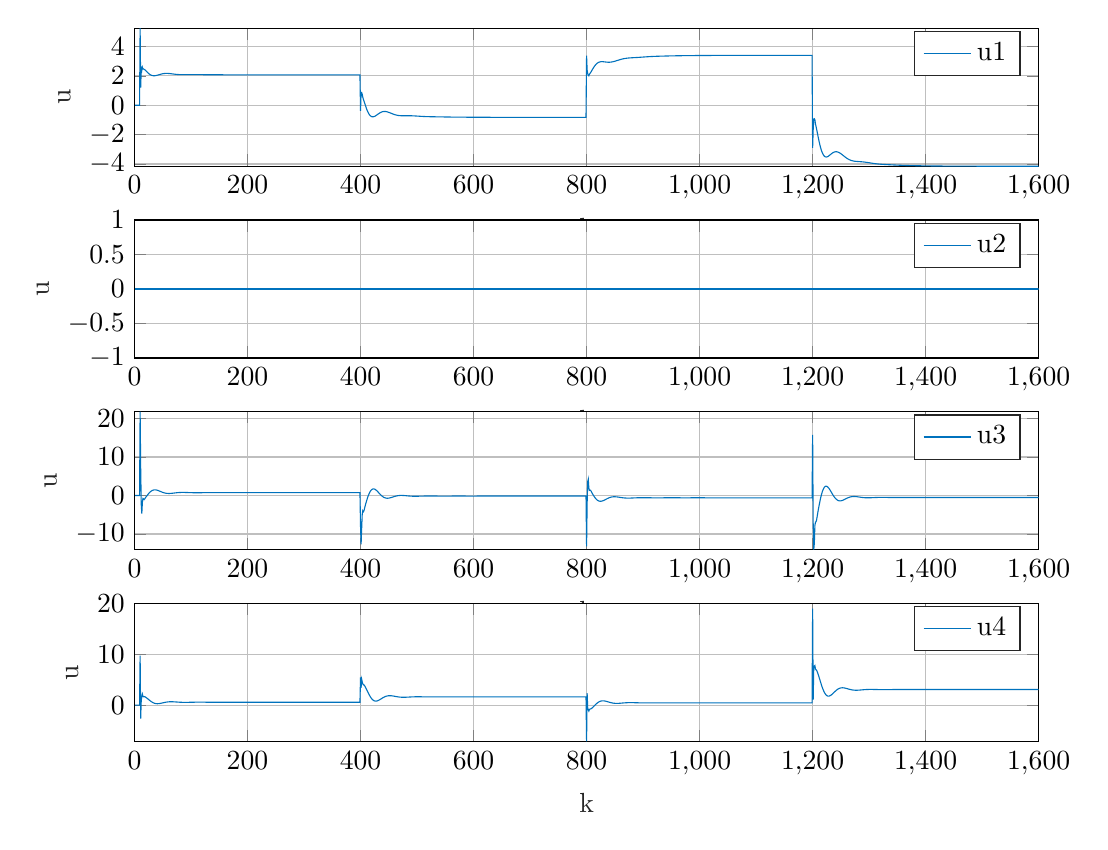
\begin{tikzpicture}

\begin{axis}[%
width=4.521in,
height=0.69in,
at={(0.758in,3.357in)},
scale only axis,
xmin=0,
xmax=1600,
xlabel style={font=\color{white!15!black}},
xlabel={k},
ymin=-4.1506,
ymax=5.2469,
ylabel style={font=\color{white!15!black}},
ylabel={u},
axis background/.style={fill=white},
xmajorgrids,
ymajorgrids,
legend style={legend cell align=left, align=left, draw=white!15!black}
]
\addplot [color=mycolor1]
  table[row sep=crcr]{%
1	0\\
2	0\\
3	0\\
4	0\\
5	0\\
6	0\\
7	0\\
8	0\\
9	0\\
10	5.2469\\
11	1.211\\
12	2.5198\\
13	2.3708\\
14	2.5901\\
15	2.4821\\
16	2.4711\\
17	2.4461\\
18	2.4273\\
19	2.3927\\
20	2.3544\\
21	2.3145\\
22	2.2754\\
23	2.237\\
24	2.2003\\
25	2.1658\\
26	2.1344\\
27	2.1062\\
28	2.0817\\
29	2.0609\\
30	2.0438\\
31	2.0305\\
32	2.0207\\
33	2.0144\\
34	2.0112\\
35	2.011\\
36	2.0133\\
37	2.018\\
38	2.0246\\
39	2.0329\\
40	2.0424\\
41	2.0529\\
42	2.0641\\
43	2.0756\\
44	2.0872\\
45	2.0987\\
46	2.1097\\
47	2.1202\\
48	2.13\\
49	2.1389\\
50	2.1468\\
51	2.1536\\
52	2.1594\\
53	2.164\\
54	2.1675\\
55	2.1699\\
56	2.1712\\
57	2.1715\\
58	2.1709\\
59	2.1693\\
60	2.167\\
61	2.164\\
62	2.1604\\
63	2.1563\\
64	2.1518\\
65	2.1471\\
66	2.1421\\
67	2.137\\
68	2.1319\\
69	2.1268\\
70	2.1219\\
71	2.1172\\
72	2.1127\\
73	2.1084\\
74	2.1045\\
75	2.1009\\
76	2.0977\\
77	2.0949\\
78	2.0924\\
79	2.0903\\
80	2.0886\\
81	2.0872\\
82	2.0861\\
83	2.0854\\
84	2.0849\\
85	2.0847\\
86	2.0847\\
87	2.0848\\
88	2.0852\\
89	2.0856\\
90	2.0862\\
91	2.0869\\
92	2.0875\\
93	2.0882\\
94	2.0889\\
95	2.0896\\
96	2.0902\\
97	2.0908\\
98	2.0913\\
99	2.0917\\
100	2.092\\
101	2.0923\\
102	2.0924\\
103	2.0924\\
104	2.0924\\
105	2.0922\\
106	2.092\\
107	2.0917\\
108	2.0913\\
109	2.0908\\
110	2.0903\\
111	2.0897\\
112	2.0891\\
113	2.0884\\
114	2.0878\\
115	2.0871\\
116	2.0864\\
117	2.0857\\
118	2.085\\
119	2.0843\\
120	2.0837\\
121	2.0831\\
122	2.0825\\
123	2.0819\\
124	2.0813\\
125	2.0808\\
126	2.0804\\
127	2.08\\
128	2.0796\\
129	2.0792\\
130	2.0789\\
131	2.0786\\
132	2.0784\\
133	2.0781\\
134	2.0779\\
135	2.0778\\
136	2.0776\\
137	2.0775\\
138	2.0774\\
139	2.0773\\
140	2.0772\\
141	2.0771\\
142	2.077\\
143	2.0769\\
144	2.0768\\
145	2.0768\\
146	2.0767\\
147	2.0766\\
148	2.0765\\
149	2.0764\\
150	2.0763\\
151	2.0762\\
152	2.0761\\
153	2.076\\
154	2.0758\\
155	2.0757\\
156	2.0756\\
157	2.0754\\
158	2.0753\\
159	2.0751\\
160	2.075\\
161	2.0748\\
162	2.0747\\
163	2.0745\\
164	2.0744\\
165	2.0742\\
166	2.0741\\
167	2.0739\\
168	2.0738\\
169	2.0736\\
170	2.0735\\
171	2.0733\\
172	2.0732\\
173	2.0731\\
174	2.073\\
175	2.0728\\
176	2.0727\\
177	2.0726\\
178	2.0725\\
179	2.0724\\
180	2.0723\\
181	2.0722\\
182	2.0722\\
183	2.0721\\
184	2.072\\
185	2.0719\\
186	2.0719\\
187	2.0718\\
188	2.0717\\
189	2.0717\\
190	2.0716\\
191	2.0715\\
192	2.0715\\
193	2.0714\\
194	2.0714\\
195	2.0713\\
196	2.0712\\
197	2.0712\\
198	2.0711\\
199	2.0711\\
200	2.071\\
201	2.071\\
202	2.0709\\
203	2.0709\\
204	2.0708\\
205	2.0708\\
206	2.0707\\
207	2.0707\\
208	2.0706\\
209	2.0706\\
210	2.0705\\
211	2.0705\\
212	2.0704\\
213	2.0704\\
214	2.0703\\
215	2.0703\\
216	2.0702\\
217	2.0702\\
218	2.0702\\
219	2.0701\\
220	2.0701\\
221	2.07\\
222	2.07\\
223	2.07\\
224	2.0699\\
225	2.0699\\
226	2.0698\\
227	2.0698\\
228	2.0698\\
229	2.0697\\
230	2.0697\\
231	2.0697\\
232	2.0697\\
233	2.0696\\
234	2.0696\\
235	2.0696\\
236	2.0695\\
237	2.0695\\
238	2.0695\\
239	2.0695\\
240	2.0694\\
241	2.0694\\
242	2.0694\\
243	2.0694\\
244	2.0694\\
245	2.0693\\
246	2.0693\\
247	2.0693\\
248	2.0693\\
249	2.0693\\
250	2.0692\\
251	2.0692\\
252	2.0692\\
253	2.0692\\
254	2.0692\\
255	2.0691\\
256	2.0691\\
257	2.0691\\
258	2.0691\\
259	2.0691\\
260	2.0691\\
261	2.069\\
262	2.069\\
263	2.069\\
264	2.069\\
265	2.069\\
266	2.069\\
267	2.0689\\
268	2.0689\\
269	2.0689\\
270	2.0689\\
271	2.0689\\
272	2.0689\\
273	2.0689\\
274	2.0689\\
275	2.0688\\
276	2.0688\\
277	2.0688\\
278	2.0688\\
279	2.0688\\
280	2.0688\\
281	2.0688\\
282	2.0688\\
283	2.0688\\
284	2.0687\\
285	2.0687\\
286	2.0687\\
287	2.0687\\
288	2.0687\\
289	2.0687\\
290	2.0687\\
291	2.0687\\
292	2.0687\\
293	2.0687\\
294	2.0687\\
295	2.0687\\
296	2.0686\\
297	2.0686\\
298	2.0686\\
299	2.0686\\
300	2.0686\\
301	2.0686\\
302	2.0686\\
303	2.0686\\
304	2.0686\\
305	2.0686\\
306	2.0686\\
307	2.0686\\
308	2.0686\\
309	2.0686\\
310	2.0686\\
311	2.0686\\
312	2.0685\\
313	2.0685\\
314	2.0685\\
315	2.0685\\
316	2.0685\\
317	2.0685\\
318	2.0685\\
319	2.0685\\
320	2.0685\\
321	2.0685\\
322	2.0685\\
323	2.0685\\
324	2.0685\\
325	2.0685\\
326	2.0685\\
327	2.0685\\
328	2.0685\\
329	2.0685\\
330	2.0685\\
331	2.0685\\
332	2.0685\\
333	2.0685\\
334	2.0685\\
335	2.0685\\
336	2.0685\\
337	2.0684\\
338	2.0684\\
339	2.0684\\
340	2.0684\\
341	2.0684\\
342	2.0684\\
343	2.0684\\
344	2.0684\\
345	2.0684\\
346	2.0684\\
347	2.0684\\
348	2.0684\\
349	2.0684\\
350	2.0684\\
351	2.0684\\
352	2.0684\\
353	2.0684\\
354	2.0684\\
355	2.0684\\
356	2.0684\\
357	2.0684\\
358	2.0684\\
359	2.0684\\
360	2.0684\\
361	2.0684\\
362	2.0684\\
363	2.0684\\
364	2.0684\\
365	2.0684\\
366	2.0684\\
367	2.0684\\
368	2.0684\\
369	2.0684\\
370	2.0684\\
371	2.0684\\
372	2.0684\\
373	2.0684\\
374	2.0684\\
375	2.0684\\
376	2.0684\\
377	2.0684\\
378	2.0684\\
379	2.0684\\
380	2.0684\\
381	2.0684\\
382	2.0684\\
383	2.0684\\
384	2.0684\\
385	2.0684\\
386	2.0684\\
387	2.0684\\
388	2.0684\\
389	2.0684\\
390	2.0684\\
391	2.0684\\
392	2.0684\\
393	2.0683\\
394	2.0683\\
395	2.0683\\
396	2.0683\\
397	2.0683\\
398	2.0683\\
399	2.0683\\
400	-0.38019\\
401	0.83675\\
402	0.86817\\
403	0.7445\\
404	0.55514\\
405	0.41687\\
406	0.30755\\
407	0.18852\\
408	0.065139\\
409	-0.055088\\
410	-0.16726\\
411	-0.27132\\
412	-0.36692\\
413	-0.45328\\
414	-0.52963\\
415	-0.59562\\
416	-0.65121\\
417	-0.69653\\
418	-0.73188\\
419	-0.75771\\
420	-0.7746\\
421	-0.78324\\
422	-0.7844\\
423	-0.7789\\
424	-0.76763\\
425	-0.75146\\
426	-0.7313\\
427	-0.70801\\
428	-0.68245\\
429	-0.65542\\
430	-0.62769\\
431	-0.59994\\
432	-0.5728\\
433	-0.54684\\
434	-0.52252\\
435	-0.50025\\
436	-0.48037\\
437	-0.46311\\
438	-0.44867\\
439	-0.43714\\
440	-0.42858\\
441	-0.42297\\
442	-0.42024\\
443	-0.42027\\
444	-0.42292\\
445	-0.42798\\
446	-0.43524\\
447	-0.44447\\
448	-0.45541\\
449	-0.4678\\
450	-0.48137\\
451	-0.49585\\
452	-0.511\\
453	-0.52656\\
454	-0.5423\\
455	-0.558\\
456	-0.57347\\
457	-0.58852\\
458	-0.60302\\
459	-0.61681\\
460	-0.6298\\
461	-0.64189\\
462	-0.65303\\
463	-0.66318\\
464	-0.6723\\
465	-0.6804\\
466	-0.68749\\
467	-0.6936\\
468	-0.69877\\
469	-0.70306\\
470	-0.70652\\
471	-0.70924\\
472	-0.71128\\
473	-0.71273\\
474	-0.71367\\
475	-0.71418\\
476	-0.71433\\
477	-0.71422\\
478	-0.71391\\
479	-0.71348\\
480	-0.71299\\
481	-0.71249\\
482	-0.71204\\
483	-0.7117\\
484	-0.71149\\
485	-0.71144\\
486	-0.71159\\
487	-0.71195\\
488	-0.71253\\
489	-0.71335\\
490	-0.71439\\
491	-0.71566\\
492	-0.71714\\
493	-0.71883\\
494	-0.72071\\
495	-0.72276\\
496	-0.72496\\
497	-0.72729\\
498	-0.72972\\
499	-0.73224\\
500	-0.73481\\
501	-0.73742\\
502	-0.74005\\
503	-0.74267\\
504	-0.74527\\
505	-0.74782\\
506	-0.75031\\
507	-0.75273\\
508	-0.75507\\
509	-0.75731\\
510	-0.75945\\
511	-0.76148\\
512	-0.76341\\
513	-0.76522\\
514	-0.76691\\
515	-0.7685\\
516	-0.76997\\
517	-0.77135\\
518	-0.77262\\
519	-0.7738\\
520	-0.77489\\
521	-0.7759\\
522	-0.77683\\
523	-0.77771\\
524	-0.77852\\
525	-0.77929\\
526	-0.78001\\
527	-0.7807\\
528	-0.78136\\
529	-0.782\\
530	-0.78263\\
531	-0.78324\\
532	-0.78385\\
533	-0.78445\\
534	-0.78506\\
535	-0.78567\\
536	-0.78628\\
537	-0.7869\\
538	-0.78753\\
539	-0.78817\\
540	-0.78882\\
541	-0.78948\\
542	-0.79014\\
543	-0.79081\\
544	-0.79148\\
545	-0.79216\\
546	-0.79284\\
547	-0.79352\\
548	-0.79419\\
549	-0.79487\\
550	-0.79553\\
551	-0.79619\\
552	-0.79684\\
553	-0.79748\\
554	-0.79811\\
555	-0.79872\\
556	-0.79932\\
557	-0.79991\\
558	-0.80047\\
559	-0.80102\\
560	-0.80156\\
561	-0.80207\\
562	-0.80257\\
563	-0.80305\\
564	-0.80352\\
565	-0.80396\\
566	-0.80439\\
567	-0.80481\\
568	-0.80521\\
569	-0.80559\\
570	-0.80597\\
571	-0.80633\\
572	-0.80668\\
573	-0.80701\\
574	-0.80734\\
575	-0.80766\\
576	-0.80796\\
577	-0.80827\\
578	-0.80856\\
579	-0.80885\\
580	-0.80913\\
581	-0.8094\\
582	-0.80967\\
583	-0.80994\\
584	-0.8102\\
585	-0.81046\\
586	-0.81071\\
587	-0.81096\\
588	-0.81121\\
589	-0.81145\\
590	-0.81169\\
591	-0.81193\\
592	-0.81216\\
593	-0.81239\\
594	-0.81262\\
595	-0.81284\\
596	-0.81306\\
597	-0.81328\\
598	-0.81349\\
599	-0.8137\\
600	-0.81391\\
601	-0.81411\\
602	-0.81431\\
603	-0.8145\\
604	-0.81469\\
605	-0.81487\\
606	-0.81506\\
607	-0.81523\\
608	-0.81541\\
609	-0.81557\\
610	-0.81574\\
611	-0.8159\\
612	-0.81605\\
613	-0.81621\\
614	-0.81635\\
615	-0.8165\\
616	-0.81664\\
617	-0.81678\\
618	-0.81691\\
619	-0.81704\\
620	-0.81717\\
621	-0.81729\\
622	-0.81741\\
623	-0.81753\\
624	-0.81765\\
625	-0.81776\\
626	-0.81787\\
627	-0.81798\\
628	-0.81808\\
629	-0.81819\\
630	-0.81829\\
631	-0.81839\\
632	-0.81848\\
633	-0.81858\\
634	-0.81867\\
635	-0.81876\\
636	-0.81885\\
637	-0.81894\\
638	-0.81903\\
639	-0.81911\\
640	-0.81919\\
641	-0.81928\\
642	-0.81935\\
643	-0.81943\\
644	-0.81951\\
645	-0.81958\\
646	-0.81966\\
647	-0.81973\\
648	-0.8198\\
649	-0.81987\\
650	-0.81994\\
651	-0.82\\
652	-0.82007\\
653	-0.82013\\
654	-0.82019\\
655	-0.82025\\
656	-0.82031\\
657	-0.82037\\
658	-0.82043\\
659	-0.82048\\
660	-0.82054\\
661	-0.82059\\
662	-0.82064\\
663	-0.82069\\
664	-0.82074\\
665	-0.82079\\
666	-0.82084\\
667	-0.82088\\
668	-0.82093\\
669	-0.82097\\
670	-0.82102\\
671	-0.82106\\
672	-0.8211\\
673	-0.82114\\
674	-0.82118\\
675	-0.82122\\
676	-0.82126\\
677	-0.82129\\
678	-0.82133\\
679	-0.82137\\
680	-0.8214\\
681	-0.82143\\
682	-0.82147\\
683	-0.8215\\
684	-0.82153\\
685	-0.82156\\
686	-0.82159\\
687	-0.82162\\
688	-0.82165\\
689	-0.82168\\
690	-0.82171\\
691	-0.82174\\
692	-0.82176\\
693	-0.82179\\
694	-0.82182\\
695	-0.82184\\
696	-0.82187\\
697	-0.82189\\
698	-0.82191\\
699	-0.82194\\
700	-0.82196\\
701	-0.82198\\
702	-0.822\\
703	-0.82202\\
704	-0.82204\\
705	-0.82207\\
706	-0.82209\\
707	-0.8221\\
708	-0.82212\\
709	-0.82214\\
710	-0.82216\\
711	-0.82218\\
712	-0.8222\\
713	-0.82221\\
714	-0.82223\\
715	-0.82225\\
716	-0.82226\\
717	-0.82228\\
718	-0.82229\\
719	-0.82231\\
720	-0.82232\\
721	-0.82234\\
722	-0.82235\\
723	-0.82236\\
724	-0.82238\\
725	-0.82239\\
726	-0.8224\\
727	-0.82242\\
728	-0.82243\\
729	-0.82244\\
730	-0.82245\\
731	-0.82246\\
732	-0.82248\\
733	-0.82249\\
734	-0.8225\\
735	-0.82251\\
736	-0.82252\\
737	-0.82253\\
738	-0.82254\\
739	-0.82255\\
740	-0.82256\\
741	-0.82257\\
742	-0.82258\\
743	-0.82258\\
744	-0.82259\\
745	-0.8226\\
746	-0.82261\\
747	-0.82262\\
748	-0.82263\\
749	-0.82263\\
750	-0.82264\\
751	-0.82265\\
752	-0.82266\\
753	-0.82266\\
754	-0.82267\\
755	-0.82268\\
756	-0.82268\\
757	-0.82269\\
758	-0.8227\\
759	-0.8227\\
760	-0.82271\\
761	-0.82272\\
762	-0.82272\\
763	-0.82273\\
764	-0.82273\\
765	-0.82274\\
766	-0.82274\\
767	-0.82275\\
768	-0.82275\\
769	-0.82276\\
770	-0.82276\\
771	-0.82277\\
772	-0.82277\\
773	-0.82278\\
774	-0.82278\\
775	-0.82279\\
776	-0.82279\\
777	-0.8228\\
778	-0.8228\\
779	-0.8228\\
780	-0.82281\\
781	-0.82281\\
782	-0.82282\\
783	-0.82282\\
784	-0.82282\\
785	-0.82283\\
786	-0.82283\\
787	-0.82283\\
788	-0.82284\\
789	-0.82284\\
790	-0.82284\\
791	-0.82285\\
792	-0.82285\\
793	-0.82285\\
794	-0.82286\\
795	-0.82286\\
796	-0.82286\\
797	-0.82286\\
798	-0.82287\\
799	-0.82287\\
800	3.3746\\
801	2.3978\\
802	2.1591\\
803	2.03\\
804	2.0025\\
805	2.108\\
806	2.1639\\
807	2.2232\\
808	2.281\\
809	2.3476\\
810	2.4146\\
811	2.4802\\
812	2.5429\\
813	2.6026\\
814	2.6586\\
815	2.7102\\
816	2.757\\
817	2.7989\\
818	2.8357\\
819	2.8675\\
820	2.8945\\
821	2.9167\\
822	2.9345\\
823	2.9483\\
824	2.9583\\
825	2.9651\\
826	2.9689\\
827	2.9703\\
828	2.9696\\
829	2.9673\\
830	2.9638\\
831	2.9595\\
832	2.9547\\
833	2.9497\\
834	2.945\\
835	2.9406\\
836	2.9369\\
837	2.9341\\
838	2.9322\\
839	2.9314\\
840	2.9318\\
841	2.9335\\
842	2.9364\\
843	2.9406\\
844	2.9459\\
845	2.9524\\
846	2.96\\
847	2.9686\\
848	2.978\\
849	2.9882\\
850	2.9991\\
851	3.0105\\
852	3.0223\\
853	3.0344\\
854	3.0466\\
855	3.0589\\
856	3.0711\\
857	3.0831\\
858	3.0949\\
859	3.1064\\
860	3.1175\\
861	3.1281\\
862	3.1382\\
863	3.1478\\
864	3.1568\\
865	3.1653\\
866	3.1732\\
867	3.1804\\
868	3.1872\\
869	3.1934\\
870	3.199\\
871	3.2042\\
872	3.2089\\
873	3.2132\\
874	3.217\\
875	3.2206\\
876	3.2238\\
877	3.2268\\
878	3.2296\\
879	3.2322\\
880	3.2346\\
881	3.2369\\
882	3.2392\\
883	3.2414\\
884	3.2435\\
885	3.2457\\
886	3.2479\\
887	3.2501\\
888	3.2524\\
889	3.2547\\
890	3.257\\
891	3.2595\\
892	3.262\\
893	3.2646\\
894	3.2672\\
895	3.2699\\
896	3.2726\\
897	3.2754\\
898	3.2782\\
899	3.281\\
900	3.2838\\
901	3.2866\\
902	3.2894\\
903	3.2922\\
904	3.295\\
905	3.2977\\
906	3.3004\\
907	3.303\\
908	3.3056\\
909	3.3081\\
910	3.3105\\
911	3.3128\\
912	3.3151\\
913	3.3173\\
914	3.3194\\
915	3.3214\\
916	3.3234\\
917	3.3252\\
918	3.327\\
919	3.3287\\
920	3.3304\\
921	3.332\\
922	3.3335\\
923	3.3349\\
924	3.3363\\
925	3.3377\\
926	3.339\\
927	3.3402\\
928	3.3415\\
929	3.3426\\
930	3.3438\\
931	3.3449\\
932	3.346\\
933	3.3471\\
934	3.3482\\
935	3.3492\\
936	3.3502\\
937	3.3512\\
938	3.3522\\
939	3.3532\\
940	3.3542\\
941	3.3552\\
942	3.3561\\
943	3.3571\\
944	3.358\\
945	3.3589\\
946	3.3598\\
947	3.3607\\
948	3.3616\\
949	3.3625\\
950	3.3634\\
951	3.3642\\
952	3.3651\\
953	3.3659\\
954	3.3667\\
955	3.3675\\
956	3.3682\\
957	3.369\\
958	3.3697\\
959	3.3705\\
960	3.3712\\
961	3.3718\\
962	3.3725\\
963	3.3732\\
964	3.3738\\
965	3.3744\\
966	3.375\\
967	3.3756\\
968	3.3762\\
969	3.3767\\
970	3.3773\\
971	3.3778\\
972	3.3783\\
973	3.3788\\
974	3.3793\\
975	3.3797\\
976	3.3802\\
977	3.3807\\
978	3.3811\\
979	3.3815\\
980	3.3819\\
981	3.3824\\
982	3.3828\\
983	3.3832\\
984	3.3835\\
985	3.3839\\
986	3.3843\\
987	3.3846\\
988	3.385\\
989	3.3854\\
990	3.3857\\
991	3.386\\
992	3.3864\\
993	3.3867\\
994	3.387\\
995	3.3873\\
996	3.3876\\
997	3.3879\\
998	3.3882\\
999	3.3885\\
1000	3.3888\\
1001	3.3891\\
1002	3.3893\\
1003	3.3896\\
1004	3.3899\\
1005	3.3901\\
1006	3.3904\\
1007	3.3906\\
1008	3.3908\\
1009	3.3911\\
1010	3.3913\\
1011	3.3915\\
1012	3.3918\\
1013	3.392\\
1014	3.3922\\
1015	3.3924\\
1016	3.3926\\
1017	3.3928\\
1018	3.393\\
1019	3.3931\\
1020	3.3933\\
1021	3.3935\\
1022	3.3937\\
1023	3.3938\\
1024	3.394\\
1025	3.3942\\
1026	3.3943\\
1027	3.3945\\
1028	3.3946\\
1029	3.3948\\
1030	3.3949\\
1031	3.3951\\
1032	3.3952\\
1033	3.3953\\
1034	3.3955\\
1035	3.3956\\
1036	3.3957\\
1037	3.3959\\
1038	3.396\\
1039	3.3961\\
1040	3.3962\\
1041	3.3963\\
1042	3.3964\\
1043	3.3965\\
1044	3.3967\\
1045	3.3968\\
1046	3.3969\\
1047	3.397\\
1048	3.3971\\
1049	3.3972\\
1050	3.3973\\
1051	3.3973\\
1052	3.3974\\
1053	3.3975\\
1054	3.3976\\
1055	3.3977\\
1056	3.3978\\
1057	3.3979\\
1058	3.3979\\
1059	3.398\\
1060	3.3981\\
1061	3.3982\\
1062	3.3982\\
1063	3.3983\\
1064	3.3984\\
1065	3.3984\\
1066	3.3985\\
1067	3.3986\\
1068	3.3986\\
1069	3.3987\\
1070	3.3988\\
1071	3.3988\\
1072	3.3989\\
1073	3.3989\\
1074	3.399\\
1075	3.3991\\
1076	3.3991\\
1077	3.3992\\
1078	3.3992\\
1079	3.3993\\
1080	3.3993\\
1081	3.3994\\
1082	3.3994\\
1083	3.3995\\
1084	3.3995\\
1085	3.3995\\
1086	3.3996\\
1087	3.3996\\
1088	3.3997\\
1089	3.3997\\
1090	3.3997\\
1091	3.3998\\
1092	3.3998\\
1093	3.3999\\
1094	3.3999\\
1095	3.3999\\
1096	3.4\\
1097	3.4\\
1098	3.4\\
1099	3.4001\\
1100	3.4001\\
1101	3.4001\\
1102	3.4002\\
1103	3.4002\\
1104	3.4002\\
1105	3.4002\\
1106	3.4003\\
1107	3.4003\\
1108	3.4003\\
1109	3.4004\\
1110	3.4004\\
1111	3.4004\\
1112	3.4004\\
1113	3.4005\\
1114	3.4005\\
1115	3.4005\\
1116	3.4005\\
1117	3.4005\\
1118	3.4006\\
1119	3.4006\\
1120	3.4006\\
1121	3.4006\\
1122	3.4007\\
1123	3.4007\\
1124	3.4007\\
1125	3.4007\\
1126	3.4007\\
1127	3.4007\\
1128	3.4008\\
1129	3.4008\\
1130	3.4008\\
1131	3.4008\\
1132	3.4008\\
1133	3.4008\\
1134	3.4009\\
1135	3.4009\\
1136	3.4009\\
1137	3.4009\\
1138	3.4009\\
1139	3.4009\\
1140	3.4009\\
1141	3.401\\
1142	3.401\\
1143	3.401\\
1144	3.401\\
1145	3.401\\
1146	3.401\\
1147	3.401\\
1148	3.401\\
1149	3.4011\\
1150	3.4011\\
1151	3.4011\\
1152	3.4011\\
1153	3.4011\\
1154	3.4011\\
1155	3.4011\\
1156	3.4011\\
1157	3.4011\\
1158	3.4011\\
1159	3.4011\\
1160	3.4012\\
1161	3.4012\\
1162	3.4012\\
1163	3.4012\\
1164	3.4012\\
1165	3.4012\\
1166	3.4012\\
1167	3.4012\\
1168	3.4012\\
1169	3.4012\\
1170	3.4012\\
1171	3.4012\\
1172	3.4012\\
1173	3.4013\\
1174	3.4013\\
1175	3.4013\\
1176	3.4013\\
1177	3.4013\\
1178	3.4013\\
1179	3.4013\\
1180	3.4013\\
1181	3.4013\\
1182	3.4013\\
1183	3.4013\\
1184	3.4013\\
1185	3.4013\\
1186	3.4013\\
1187	3.4013\\
1188	3.4013\\
1189	3.4013\\
1190	3.4013\\
1191	3.4014\\
1192	3.4014\\
1193	3.4014\\
1194	3.4014\\
1195	3.4014\\
1196	3.4014\\
1197	3.4014\\
1198	3.4014\\
1199	3.4014\\
1200	-2.8948\\
1201	-1.6506\\
1202	-0.95014\\
1203	-0.91758\\
1204	-0.97796\\
1205	-1.264\\
1206	-1.433\\
1207	-1.6184\\
1208	-1.8036\\
1209	-2.0025\\
1210	-2.1962\\
1211	-2.3817\\
1212	-2.5562\\
1213	-2.7187\\
1214	-2.8674\\
1215	-3.001\\
1216	-3.1188\\
1217	-3.2205\\
1218	-3.3061\\
1219	-3.3761\\
1220	-3.4311\\
1221	-3.472\\
1222	-3.4997\\
1223	-3.5155\\
1224	-3.5206\\
1225	-3.5164\\
1226	-3.5043\\
1227	-3.4856\\
1228	-3.4618\\
1229	-3.4341\\
1230	-3.4039\\
1231	-3.3723\\
1232	-3.3404\\
1233	-3.3091\\
1234	-3.2794\\
1235	-3.2521\\
1236	-3.2277\\
1237	-3.2067\\
1238	-3.1896\\
1239	-3.1767\\
1240	-3.168\\
1241	-3.1638\\
1242	-3.1639\\
1243	-3.1683\\
1244	-3.1768\\
1245	-3.1892\\
1246	-3.2051\\
1247	-3.2243\\
1248	-3.2463\\
1249	-3.2708\\
1250	-3.2973\\
1251	-3.3255\\
1252	-3.3549\\
1253	-3.3852\\
1254	-3.416\\
1255	-3.4469\\
1256	-3.4775\\
1257	-3.5076\\
1258	-3.537\\
1259	-3.5652\\
1260	-3.5923\\
1261	-3.6179\\
1262	-3.6421\\
1263	-3.6646\\
1264	-3.6854\\
1265	-3.7045\\
1266	-3.7218\\
1267	-3.7375\\
1268	-3.7516\\
1269	-3.764\\
1270	-3.775\\
1271	-3.7846\\
1272	-3.793\\
1273	-3.8002\\
1274	-3.8063\\
1275	-3.8116\\
1276	-3.8162\\
1277	-3.82\\
1278	-3.8234\\
1279	-3.8264\\
1280	-3.8292\\
1281	-3.8317\\
1282	-3.8342\\
1283	-3.8367\\
1284	-3.8393\\
1285	-3.842\\
1286	-3.8449\\
1287	-3.8481\\
1288	-3.8515\\
1289	-3.8552\\
1290	-3.8592\\
1291	-3.8635\\
1292	-3.868\\
1293	-3.8729\\
1294	-3.878\\
1295	-3.8834\\
1296	-3.889\\
1297	-3.8947\\
1298	-3.9006\\
1299	-3.9066\\
1300	-3.9127\\
1301	-3.9189\\
1302	-3.925\\
1303	-3.9311\\
1304	-3.9372\\
1305	-3.9432\\
1306	-3.949\\
1307	-3.9548\\
1308	-3.9604\\
1309	-3.9658\\
1310	-3.971\\
1311	-3.976\\
1312	-3.9808\\
1313	-3.9854\\
1314	-3.9898\\
1315	-3.994\\
1316	-3.998\\
1317	-4.0018\\
1318	-4.0054\\
1319	-4.0087\\
1320	-4.012\\
1321	-4.015\\
1322	-4.0179\\
1323	-4.0206\\
1324	-4.0233\\
1325	-4.0258\\
1326	-4.0282\\
1327	-4.0305\\
1328	-4.0327\\
1329	-4.0349\\
1330	-4.037\\
1331	-4.039\\
1332	-4.041\\
1333	-4.043\\
1334	-4.045\\
1335	-4.0469\\
1336	-4.0488\\
1337	-4.0507\\
1338	-4.0526\\
1339	-4.0545\\
1340	-4.0564\\
1341	-4.0583\\
1342	-4.0602\\
1343	-4.062\\
1344	-4.0639\\
1345	-4.0657\\
1346	-4.0676\\
1347	-4.0694\\
1348	-4.0712\\
1349	-4.073\\
1350	-4.0747\\
1351	-4.0765\\
1352	-4.0782\\
1353	-4.0799\\
1354	-4.0815\\
1355	-4.0831\\
1356	-4.0847\\
1357	-4.0862\\
1358	-4.0878\\
1359	-4.0892\\
1360	-4.0906\\
1361	-4.092\\
1362	-4.0934\\
1363	-4.0947\\
1364	-4.096\\
1365	-4.0972\\
1366	-4.0984\\
1367	-4.0996\\
1368	-4.1007\\
1369	-4.1018\\
1370	-4.1029\\
1371	-4.1039\\
1372	-4.1049\\
1373	-4.1059\\
1374	-4.1068\\
1375	-4.1077\\
1376	-4.1086\\
1377	-4.1095\\
1378	-4.1104\\
1379	-4.1112\\
1380	-4.112\\
1381	-4.1128\\
1382	-4.1136\\
1383	-4.1144\\
1384	-4.1151\\
1385	-4.1158\\
1386	-4.1166\\
1387	-4.1173\\
1388	-4.118\\
1389	-4.1187\\
1390	-4.1194\\
1391	-4.12\\
1392	-4.1207\\
1393	-4.1213\\
1394	-4.1219\\
1395	-4.1226\\
1396	-4.1232\\
1397	-4.1238\\
1398	-4.1244\\
1399	-4.1249\\
1400	-4.1255\\
1401	-4.1261\\
1402	-4.1266\\
1403	-4.1271\\
1404	-4.1277\\
1405	-4.1282\\
1406	-4.1287\\
1407	-4.1292\\
1408	-4.1296\\
1409	-4.1301\\
1410	-4.1306\\
1411	-4.131\\
1412	-4.1314\\
1413	-4.1319\\
1414	-4.1323\\
1415	-4.1327\\
1416	-4.1331\\
1417	-4.1335\\
1418	-4.1338\\
1419	-4.1342\\
1420	-4.1346\\
1421	-4.1349\\
1422	-4.1352\\
1423	-4.1356\\
1424	-4.1359\\
1425	-4.1362\\
1426	-4.1365\\
1427	-4.1368\\
1428	-4.1371\\
1429	-4.1374\\
1430	-4.1377\\
1431	-4.138\\
1432	-4.1383\\
1433	-4.1385\\
1434	-4.1388\\
1435	-4.1391\\
1436	-4.1393\\
1437	-4.1396\\
1438	-4.1398\\
1439	-4.14\\
1440	-4.1403\\
1441	-4.1405\\
1442	-4.1407\\
1443	-4.1409\\
1444	-4.1411\\
1445	-4.1414\\
1446	-4.1416\\
1447	-4.1418\\
1448	-4.142\\
1449	-4.1421\\
1450	-4.1423\\
1451	-4.1425\\
1452	-4.1427\\
1453	-4.1429\\
1454	-4.1431\\
1455	-4.1432\\
1456	-4.1434\\
1457	-4.1435\\
1458	-4.1437\\
1459	-4.1439\\
1460	-4.144\\
1461	-4.1442\\
1462	-4.1443\\
1463	-4.1444\\
1464	-4.1446\\
1465	-4.1447\\
1466	-4.1449\\
1467	-4.145\\
1468	-4.1451\\
1469	-4.1452\\
1470	-4.1454\\
1471	-4.1455\\
1472	-4.1456\\
1473	-4.1457\\
1474	-4.1458\\
1475	-4.1459\\
1476	-4.146\\
1477	-4.1461\\
1478	-4.1462\\
1479	-4.1463\\
1480	-4.1464\\
1481	-4.1465\\
1482	-4.1466\\
1483	-4.1467\\
1484	-4.1468\\
1485	-4.1469\\
1486	-4.147\\
1487	-4.1471\\
1488	-4.1471\\
1489	-4.1472\\
1490	-4.1473\\
1491	-4.1474\\
1492	-4.1475\\
1493	-4.1475\\
1494	-4.1476\\
1495	-4.1477\\
1496	-4.1477\\
1497	-4.1478\\
1498	-4.1479\\
1499	-4.1479\\
1500	-4.148\\
1501	-4.1481\\
1502	-4.1481\\
1503	-4.1482\\
1504	-4.1482\\
1505	-4.1483\\
1506	-4.1484\\
1507	-4.1484\\
1508	-4.1485\\
1509	-4.1485\\
1510	-4.1486\\
1511	-4.1486\\
1512	-4.1487\\
1513	-4.1487\\
1514	-4.1488\\
1515	-4.1488\\
1516	-4.1488\\
1517	-4.1489\\
1518	-4.1489\\
1519	-4.149\\
1520	-4.149\\
1521	-4.1491\\
1522	-4.1491\\
1523	-4.1491\\
1524	-4.1492\\
1525	-4.1492\\
1526	-4.1492\\
1527	-4.1493\\
1528	-4.1493\\
1529	-4.1493\\
1530	-4.1494\\
1531	-4.1494\\
1532	-4.1494\\
1533	-4.1495\\
1534	-4.1495\\
1535	-4.1495\\
1536	-4.1496\\
1537	-4.1496\\
1538	-4.1496\\
1539	-4.1496\\
1540	-4.1497\\
1541	-4.1497\\
1542	-4.1497\\
1543	-4.1498\\
1544	-4.1498\\
1545	-4.1498\\
1546	-4.1498\\
1547	-4.1498\\
1548	-4.1499\\
1549	-4.1499\\
1550	-4.1499\\
1551	-4.1499\\
1552	-4.15\\
1553	-4.15\\
1554	-4.15\\
1555	-4.15\\
1556	-4.15\\
1557	-4.15\\
1558	-4.1501\\
1559	-4.1501\\
1560	-4.1501\\
1561	-4.1501\\
1562	-4.1501\\
1563	-4.1502\\
1564	-4.1502\\
1565	-4.1502\\
1566	-4.1502\\
1567	-4.1502\\
1568	-4.1502\\
1569	-4.1502\\
1570	-4.1503\\
1571	-4.1503\\
1572	-4.1503\\
1573	-4.1503\\
1574	-4.1503\\
1575	-4.1503\\
1576	-4.1503\\
1577	-4.1503\\
1578	-4.1504\\
1579	-4.1504\\
1580	-4.1504\\
1581	-4.1504\\
1582	-4.1504\\
1583	-4.1504\\
1584	-4.1504\\
1585	-4.1504\\
1586	-4.1504\\
1587	-4.1504\\
1588	-4.1505\\
1589	-4.1505\\
1590	-4.1505\\
1591	-4.1505\\
1592	-4.1505\\
1593	-4.1505\\
1594	-4.1505\\
1595	-4.1505\\
1596	-4.1505\\
1597	-4.1505\\
1598	-4.1505\\
1599	-4.1505\\
1600	-4.1506\\
};
\addlegendentry{u1}

\end{axis}

\begin{axis}[%
width=4.521in,
height=0.69in,
at={(0.758in,2.398in)},
scale only axis,
xmin=0,
xmax=1600,
xlabel style={font=\color{white!15!black}},
xlabel={k},
ymin=-1,
ymax=1,
ylabel style={font=\color{white!15!black}},
ylabel={u},
axis background/.style={fill=white},
xmajorgrids,
ymajorgrids,
legend style={legend cell align=left, align=left, draw=white!15!black}
]
\addplot [color=mycolor1]
  table[row sep=crcr]{%
1	0\\
2	0\\
3	0\\
4	0\\
5	0\\
6	0\\
7	0\\
8	0\\
9	0\\
10	0\\
11	0\\
12	0\\
13	0\\
14	0\\
15	0\\
16	0\\
17	0\\
18	0\\
19	0\\
20	0\\
21	0\\
22	0\\
23	0\\
24	0\\
25	0\\
26	0\\
27	0\\
28	0\\
29	0\\
30	0\\
31	0\\
32	0\\
33	0\\
34	0\\
35	0\\
36	0\\
37	0\\
38	0\\
39	0\\
40	0\\
41	0\\
42	0\\
43	0\\
44	0\\
45	0\\
46	0\\
47	0\\
48	0\\
49	0\\
50	0\\
51	0\\
52	0\\
53	0\\
54	0\\
55	0\\
56	0\\
57	0\\
58	0\\
59	0\\
60	0\\
61	0\\
62	0\\
63	0\\
64	0\\
65	0\\
66	0\\
67	0\\
68	0\\
69	0\\
70	0\\
71	0\\
72	0\\
73	0\\
74	0\\
75	0\\
76	0\\
77	0\\
78	0\\
79	0\\
80	0\\
81	0\\
82	0\\
83	0\\
84	0\\
85	0\\
86	0\\
87	0\\
88	0\\
89	0\\
90	0\\
91	0\\
92	0\\
93	0\\
94	0\\
95	0\\
96	0\\
97	0\\
98	0\\
99	0\\
100	0\\
101	0\\
102	0\\
103	0\\
104	0\\
105	0\\
106	0\\
107	0\\
108	0\\
109	0\\
110	0\\
111	0\\
112	0\\
113	0\\
114	0\\
115	0\\
116	0\\
117	0\\
118	0\\
119	0\\
120	0\\
121	0\\
122	0\\
123	0\\
124	0\\
125	0\\
126	0\\
127	0\\
128	0\\
129	0\\
130	0\\
131	0\\
132	0\\
133	0\\
134	0\\
135	0\\
136	0\\
137	0\\
138	0\\
139	0\\
140	0\\
141	0\\
142	0\\
143	0\\
144	0\\
145	0\\
146	0\\
147	0\\
148	0\\
149	0\\
150	0\\
151	0\\
152	0\\
153	0\\
154	0\\
155	0\\
156	0\\
157	0\\
158	0\\
159	0\\
160	0\\
161	0\\
162	0\\
163	0\\
164	0\\
165	0\\
166	0\\
167	0\\
168	0\\
169	0\\
170	0\\
171	0\\
172	0\\
173	0\\
174	0\\
175	0\\
176	0\\
177	0\\
178	0\\
179	0\\
180	0\\
181	0\\
182	0\\
183	0\\
184	0\\
185	0\\
186	0\\
187	0\\
188	0\\
189	0\\
190	0\\
191	0\\
192	0\\
193	0\\
194	0\\
195	0\\
196	0\\
197	0\\
198	0\\
199	0\\
200	0\\
201	0\\
202	0\\
203	0\\
204	0\\
205	0\\
206	0\\
207	0\\
208	0\\
209	0\\
210	0\\
211	0\\
212	0\\
213	0\\
214	0\\
215	0\\
216	0\\
217	0\\
218	0\\
219	0\\
220	0\\
221	0\\
222	0\\
223	0\\
224	0\\
225	0\\
226	0\\
227	0\\
228	0\\
229	0\\
230	0\\
231	0\\
232	0\\
233	0\\
234	0\\
235	0\\
236	0\\
237	0\\
238	0\\
239	0\\
240	0\\
241	0\\
242	0\\
243	0\\
244	0\\
245	0\\
246	0\\
247	0\\
248	0\\
249	0\\
250	0\\
251	0\\
252	0\\
253	0\\
254	0\\
255	0\\
256	0\\
257	0\\
258	0\\
259	0\\
260	0\\
261	0\\
262	0\\
263	0\\
264	0\\
265	0\\
266	0\\
267	0\\
268	0\\
269	0\\
270	0\\
271	0\\
272	0\\
273	0\\
274	0\\
275	0\\
276	0\\
277	0\\
278	0\\
279	0\\
280	0\\
281	0\\
282	0\\
283	0\\
284	0\\
285	0\\
286	0\\
287	0\\
288	0\\
289	0\\
290	0\\
291	0\\
292	0\\
293	0\\
294	0\\
295	0\\
296	0\\
297	0\\
298	0\\
299	0\\
300	0\\
301	0\\
302	0\\
303	0\\
304	0\\
305	0\\
306	0\\
307	0\\
308	0\\
309	0\\
310	0\\
311	0\\
312	0\\
313	0\\
314	0\\
315	0\\
316	0\\
317	0\\
318	0\\
319	0\\
320	0\\
321	0\\
322	0\\
323	0\\
324	0\\
325	0\\
326	0\\
327	0\\
328	0\\
329	0\\
330	0\\
331	0\\
332	0\\
333	0\\
334	0\\
335	0\\
336	0\\
337	0\\
338	0\\
339	0\\
340	0\\
341	0\\
342	0\\
343	0\\
344	0\\
345	0\\
346	0\\
347	0\\
348	0\\
349	0\\
350	0\\
351	0\\
352	0\\
353	0\\
354	0\\
355	0\\
356	0\\
357	0\\
358	0\\
359	0\\
360	0\\
361	0\\
362	0\\
363	0\\
364	0\\
365	0\\
366	0\\
367	0\\
368	0\\
369	0\\
370	0\\
371	0\\
372	0\\
373	0\\
374	0\\
375	0\\
376	0\\
377	0\\
378	0\\
379	0\\
380	0\\
381	0\\
382	0\\
383	0\\
384	0\\
385	0\\
386	0\\
387	0\\
388	0\\
389	0\\
390	0\\
391	0\\
392	0\\
393	0\\
394	0\\
395	0\\
396	0\\
397	0\\
398	0\\
399	0\\
400	0\\
401	0\\
402	0\\
403	0\\
404	0\\
405	0\\
406	0\\
407	0\\
408	0\\
409	0\\
410	0\\
411	0\\
412	0\\
413	0\\
414	0\\
415	0\\
416	0\\
417	0\\
418	0\\
419	0\\
420	0\\
421	0\\
422	0\\
423	0\\
424	0\\
425	0\\
426	0\\
427	0\\
428	0\\
429	0\\
430	0\\
431	0\\
432	0\\
433	0\\
434	0\\
435	0\\
436	0\\
437	0\\
438	0\\
439	0\\
440	0\\
441	0\\
442	0\\
443	0\\
444	0\\
445	0\\
446	0\\
447	0\\
448	0\\
449	0\\
450	0\\
451	0\\
452	0\\
453	0\\
454	0\\
455	0\\
456	0\\
457	0\\
458	0\\
459	0\\
460	0\\
461	0\\
462	0\\
463	0\\
464	0\\
465	0\\
466	0\\
467	0\\
468	0\\
469	0\\
470	0\\
471	0\\
472	0\\
473	0\\
474	0\\
475	0\\
476	0\\
477	0\\
478	0\\
479	0\\
480	0\\
481	0\\
482	0\\
483	0\\
484	0\\
485	0\\
486	0\\
487	0\\
488	0\\
489	0\\
490	0\\
491	0\\
492	0\\
493	0\\
494	0\\
495	0\\
496	0\\
497	0\\
498	0\\
499	0\\
500	0\\
501	0\\
502	0\\
503	0\\
504	0\\
505	0\\
506	0\\
507	0\\
508	0\\
509	0\\
510	0\\
511	0\\
512	0\\
513	0\\
514	0\\
515	0\\
516	0\\
517	0\\
518	0\\
519	0\\
520	0\\
521	0\\
522	0\\
523	0\\
524	0\\
525	0\\
526	0\\
527	0\\
528	0\\
529	0\\
530	0\\
531	0\\
532	0\\
533	0\\
534	0\\
535	0\\
536	0\\
537	0\\
538	0\\
539	0\\
540	0\\
541	0\\
542	0\\
543	0\\
544	0\\
545	0\\
546	0\\
547	0\\
548	0\\
549	0\\
550	0\\
551	0\\
552	0\\
553	0\\
554	0\\
555	0\\
556	0\\
557	0\\
558	0\\
559	0\\
560	0\\
561	0\\
562	0\\
563	0\\
564	0\\
565	0\\
566	0\\
567	0\\
568	0\\
569	0\\
570	0\\
571	0\\
572	0\\
573	0\\
574	0\\
575	0\\
576	0\\
577	0\\
578	0\\
579	0\\
580	0\\
581	0\\
582	0\\
583	0\\
584	0\\
585	0\\
586	0\\
587	0\\
588	0\\
589	0\\
590	0\\
591	0\\
592	0\\
593	0\\
594	0\\
595	0\\
596	0\\
597	0\\
598	0\\
599	0\\
600	0\\
601	0\\
602	0\\
603	0\\
604	0\\
605	0\\
606	0\\
607	0\\
608	0\\
609	0\\
610	0\\
611	0\\
612	0\\
613	0\\
614	0\\
615	0\\
616	0\\
617	0\\
618	0\\
619	0\\
620	0\\
621	0\\
622	0\\
623	0\\
624	0\\
625	0\\
626	0\\
627	0\\
628	0\\
629	0\\
630	0\\
631	0\\
632	0\\
633	0\\
634	0\\
635	0\\
636	0\\
637	0\\
638	0\\
639	0\\
640	0\\
641	0\\
642	0\\
643	0\\
644	0\\
645	0\\
646	0\\
647	0\\
648	0\\
649	0\\
650	0\\
651	0\\
652	0\\
653	0\\
654	0\\
655	0\\
656	0\\
657	0\\
658	0\\
659	0\\
660	0\\
661	0\\
662	0\\
663	0\\
664	0\\
665	0\\
666	0\\
667	0\\
668	0\\
669	0\\
670	0\\
671	0\\
672	0\\
673	0\\
674	0\\
675	0\\
676	0\\
677	0\\
678	0\\
679	0\\
680	0\\
681	0\\
682	0\\
683	0\\
684	0\\
685	0\\
686	0\\
687	0\\
688	0\\
689	0\\
690	0\\
691	0\\
692	0\\
693	0\\
694	0\\
695	0\\
696	0\\
697	0\\
698	0\\
699	0\\
700	0\\
701	0\\
702	0\\
703	0\\
704	0\\
705	0\\
706	0\\
707	0\\
708	0\\
709	0\\
710	0\\
711	0\\
712	0\\
713	0\\
714	0\\
715	0\\
716	0\\
717	0\\
718	0\\
719	0\\
720	0\\
721	0\\
722	0\\
723	0\\
724	0\\
725	0\\
726	0\\
727	0\\
728	0\\
729	0\\
730	0\\
731	0\\
732	0\\
733	0\\
734	0\\
735	0\\
736	0\\
737	0\\
738	0\\
739	0\\
740	0\\
741	0\\
742	0\\
743	0\\
744	0\\
745	0\\
746	0\\
747	0\\
748	0\\
749	0\\
750	0\\
751	0\\
752	0\\
753	0\\
754	0\\
755	0\\
756	0\\
757	0\\
758	0\\
759	0\\
760	0\\
761	0\\
762	0\\
763	0\\
764	0\\
765	0\\
766	0\\
767	0\\
768	0\\
769	0\\
770	0\\
771	0\\
772	0\\
773	0\\
774	0\\
775	0\\
776	0\\
777	0\\
778	0\\
779	0\\
780	0\\
781	0\\
782	0\\
783	0\\
784	0\\
785	0\\
786	0\\
787	0\\
788	0\\
789	0\\
790	0\\
791	0\\
792	0\\
793	0\\
794	0\\
795	0\\
796	0\\
797	0\\
798	0\\
799	0\\
800	0\\
801	0\\
802	0\\
803	0\\
804	0\\
805	0\\
806	0\\
807	0\\
808	0\\
809	0\\
810	0\\
811	0\\
812	0\\
813	0\\
814	0\\
815	0\\
816	0\\
817	0\\
818	0\\
819	0\\
820	0\\
821	0\\
822	0\\
823	0\\
824	0\\
825	0\\
826	0\\
827	0\\
828	0\\
829	0\\
830	0\\
831	0\\
832	0\\
833	0\\
834	0\\
835	0\\
836	0\\
837	0\\
838	0\\
839	0\\
840	0\\
841	0\\
842	0\\
843	0\\
844	0\\
845	0\\
846	0\\
847	0\\
848	0\\
849	0\\
850	0\\
851	0\\
852	0\\
853	0\\
854	0\\
855	0\\
856	0\\
857	0\\
858	0\\
859	0\\
860	0\\
861	0\\
862	0\\
863	0\\
864	0\\
865	0\\
866	0\\
867	0\\
868	0\\
869	0\\
870	0\\
871	0\\
872	0\\
873	0\\
874	0\\
875	0\\
876	0\\
877	0\\
878	0\\
879	0\\
880	0\\
881	0\\
882	0\\
883	0\\
884	0\\
885	0\\
886	0\\
887	0\\
888	0\\
889	0\\
890	0\\
891	0\\
892	0\\
893	0\\
894	0\\
895	0\\
896	0\\
897	0\\
898	0\\
899	0\\
900	0\\
901	0\\
902	0\\
903	0\\
904	0\\
905	0\\
906	0\\
907	0\\
908	0\\
909	0\\
910	0\\
911	0\\
912	0\\
913	0\\
914	0\\
915	0\\
916	0\\
917	0\\
918	0\\
919	0\\
920	0\\
921	0\\
922	0\\
923	0\\
924	0\\
925	0\\
926	0\\
927	0\\
928	0\\
929	0\\
930	0\\
931	0\\
932	0\\
933	0\\
934	0\\
935	0\\
936	0\\
937	0\\
938	0\\
939	0\\
940	0\\
941	0\\
942	0\\
943	0\\
944	0\\
945	0\\
946	0\\
947	0\\
948	0\\
949	0\\
950	0\\
951	0\\
952	0\\
953	0\\
954	0\\
955	0\\
956	0\\
957	0\\
958	0\\
959	0\\
960	0\\
961	0\\
962	0\\
963	0\\
964	0\\
965	0\\
966	0\\
967	0\\
968	0\\
969	0\\
970	0\\
971	0\\
972	0\\
973	0\\
974	0\\
975	0\\
976	0\\
977	0\\
978	0\\
979	0\\
980	0\\
981	0\\
982	0\\
983	0\\
984	0\\
985	0\\
986	0\\
987	0\\
988	0\\
989	0\\
990	0\\
991	0\\
992	0\\
993	0\\
994	0\\
995	0\\
996	0\\
997	0\\
998	0\\
999	0\\
1000	0\\
1001	0\\
1002	0\\
1003	0\\
1004	0\\
1005	0\\
1006	0\\
1007	0\\
1008	0\\
1009	0\\
1010	0\\
1011	0\\
1012	0\\
1013	0\\
1014	0\\
1015	0\\
1016	0\\
1017	0\\
1018	0\\
1019	0\\
1020	0\\
1021	0\\
1022	0\\
1023	0\\
1024	0\\
1025	0\\
1026	0\\
1027	0\\
1028	0\\
1029	0\\
1030	0\\
1031	0\\
1032	0\\
1033	0\\
1034	0\\
1035	0\\
1036	0\\
1037	0\\
1038	0\\
1039	0\\
1040	0\\
1041	0\\
1042	0\\
1043	0\\
1044	0\\
1045	0\\
1046	0\\
1047	0\\
1048	0\\
1049	0\\
1050	0\\
1051	0\\
1052	0\\
1053	0\\
1054	0\\
1055	0\\
1056	0\\
1057	0\\
1058	0\\
1059	0\\
1060	0\\
1061	0\\
1062	0\\
1063	0\\
1064	0\\
1065	0\\
1066	0\\
1067	0\\
1068	0\\
1069	0\\
1070	0\\
1071	0\\
1072	0\\
1073	0\\
1074	0\\
1075	0\\
1076	0\\
1077	0\\
1078	0\\
1079	0\\
1080	0\\
1081	0\\
1082	0\\
1083	0\\
1084	0\\
1085	0\\
1086	0\\
1087	0\\
1088	0\\
1089	0\\
1090	0\\
1091	0\\
1092	0\\
1093	0\\
1094	0\\
1095	0\\
1096	0\\
1097	0\\
1098	0\\
1099	0\\
1100	0\\
1101	0\\
1102	0\\
1103	0\\
1104	0\\
1105	0\\
1106	0\\
1107	0\\
1108	0\\
1109	0\\
1110	0\\
1111	0\\
1112	0\\
1113	0\\
1114	0\\
1115	0\\
1116	0\\
1117	0\\
1118	0\\
1119	0\\
1120	0\\
1121	0\\
1122	0\\
1123	0\\
1124	0\\
1125	0\\
1126	0\\
1127	0\\
1128	0\\
1129	0\\
1130	0\\
1131	0\\
1132	0\\
1133	0\\
1134	0\\
1135	0\\
1136	0\\
1137	0\\
1138	0\\
1139	0\\
1140	0\\
1141	0\\
1142	0\\
1143	0\\
1144	0\\
1145	0\\
1146	0\\
1147	0\\
1148	0\\
1149	0\\
1150	0\\
1151	0\\
1152	0\\
1153	0\\
1154	0\\
1155	0\\
1156	0\\
1157	0\\
1158	0\\
1159	0\\
1160	0\\
1161	0\\
1162	0\\
1163	0\\
1164	0\\
1165	0\\
1166	0\\
1167	0\\
1168	0\\
1169	0\\
1170	0\\
1171	0\\
1172	0\\
1173	0\\
1174	0\\
1175	0\\
1176	0\\
1177	0\\
1178	0\\
1179	0\\
1180	0\\
1181	0\\
1182	0\\
1183	0\\
1184	0\\
1185	0\\
1186	0\\
1187	0\\
1188	0\\
1189	0\\
1190	0\\
1191	0\\
1192	0\\
1193	0\\
1194	0\\
1195	0\\
1196	0\\
1197	0\\
1198	0\\
1199	0\\
1200	0\\
1201	0\\
1202	0\\
1203	0\\
1204	0\\
1205	0\\
1206	0\\
1207	0\\
1208	0\\
1209	0\\
1210	0\\
1211	0\\
1212	0\\
1213	0\\
1214	0\\
1215	0\\
1216	0\\
1217	0\\
1218	0\\
1219	0\\
1220	0\\
1221	0\\
1222	0\\
1223	0\\
1224	0\\
1225	0\\
1226	0\\
1227	0\\
1228	0\\
1229	0\\
1230	0\\
1231	0\\
1232	0\\
1233	0\\
1234	0\\
1235	0\\
1236	0\\
1237	0\\
1238	0\\
1239	0\\
1240	0\\
1241	0\\
1242	0\\
1243	0\\
1244	0\\
1245	0\\
1246	0\\
1247	0\\
1248	0\\
1249	0\\
1250	0\\
1251	0\\
1252	0\\
1253	0\\
1254	0\\
1255	0\\
1256	0\\
1257	0\\
1258	0\\
1259	0\\
1260	0\\
1261	0\\
1262	0\\
1263	0\\
1264	0\\
1265	0\\
1266	0\\
1267	0\\
1268	0\\
1269	0\\
1270	0\\
1271	0\\
1272	0\\
1273	0\\
1274	0\\
1275	0\\
1276	0\\
1277	0\\
1278	0\\
1279	0\\
1280	0\\
1281	0\\
1282	0\\
1283	0\\
1284	0\\
1285	0\\
1286	0\\
1287	0\\
1288	0\\
1289	0\\
1290	0\\
1291	0\\
1292	0\\
1293	0\\
1294	0\\
1295	0\\
1296	0\\
1297	0\\
1298	0\\
1299	0\\
1300	0\\
1301	0\\
1302	0\\
1303	0\\
1304	0\\
1305	0\\
1306	0\\
1307	0\\
1308	0\\
1309	0\\
1310	0\\
1311	0\\
1312	0\\
1313	0\\
1314	0\\
1315	0\\
1316	0\\
1317	0\\
1318	0\\
1319	0\\
1320	0\\
1321	0\\
1322	0\\
1323	0\\
1324	0\\
1325	0\\
1326	0\\
1327	0\\
1328	0\\
1329	0\\
1330	0\\
1331	0\\
1332	0\\
1333	0\\
1334	0\\
1335	0\\
1336	0\\
1337	0\\
1338	0\\
1339	0\\
1340	0\\
1341	0\\
1342	0\\
1343	0\\
1344	0\\
1345	0\\
1346	0\\
1347	0\\
1348	0\\
1349	0\\
1350	0\\
1351	0\\
1352	0\\
1353	0\\
1354	0\\
1355	0\\
1356	0\\
1357	0\\
1358	0\\
1359	0\\
1360	0\\
1361	0\\
1362	0\\
1363	0\\
1364	0\\
1365	0\\
1366	0\\
1367	0\\
1368	0\\
1369	0\\
1370	0\\
1371	0\\
1372	0\\
1373	0\\
1374	0\\
1375	0\\
1376	0\\
1377	0\\
1378	0\\
1379	0\\
1380	0\\
1381	0\\
1382	0\\
1383	0\\
1384	0\\
1385	0\\
1386	0\\
1387	0\\
1388	0\\
1389	0\\
1390	0\\
1391	0\\
1392	0\\
1393	0\\
1394	0\\
1395	0\\
1396	0\\
1397	0\\
1398	0\\
1399	0\\
1400	0\\
1401	0\\
1402	0\\
1403	0\\
1404	0\\
1405	0\\
1406	0\\
1407	0\\
1408	0\\
1409	0\\
1410	0\\
1411	0\\
1412	0\\
1413	0\\
1414	0\\
1415	0\\
1416	0\\
1417	0\\
1418	0\\
1419	0\\
1420	0\\
1421	0\\
1422	0\\
1423	0\\
1424	0\\
1425	0\\
1426	0\\
1427	0\\
1428	0\\
1429	0\\
1430	0\\
1431	0\\
1432	0\\
1433	0\\
1434	0\\
1435	0\\
1436	0\\
1437	0\\
1438	0\\
1439	0\\
1440	0\\
1441	0\\
1442	0\\
1443	0\\
1444	0\\
1445	0\\
1446	0\\
1447	0\\
1448	0\\
1449	0\\
1450	0\\
1451	0\\
1452	0\\
1453	0\\
1454	0\\
1455	0\\
1456	0\\
1457	0\\
1458	0\\
1459	0\\
1460	0\\
1461	0\\
1462	0\\
1463	0\\
1464	0\\
1465	0\\
1466	0\\
1467	0\\
1468	0\\
1469	0\\
1470	0\\
1471	0\\
1472	0\\
1473	0\\
1474	0\\
1475	0\\
1476	0\\
1477	0\\
1478	0\\
1479	0\\
1480	0\\
1481	0\\
1482	0\\
1483	0\\
1484	0\\
1485	0\\
1486	0\\
1487	0\\
1488	0\\
1489	0\\
1490	0\\
1491	0\\
1492	0\\
1493	0\\
1494	0\\
1495	0\\
1496	0\\
1497	0\\
1498	0\\
1499	0\\
1500	0\\
1501	0\\
1502	0\\
1503	0\\
1504	0\\
1505	0\\
1506	0\\
1507	0\\
1508	0\\
1509	0\\
1510	0\\
1511	0\\
1512	0\\
1513	0\\
1514	0\\
1515	0\\
1516	0\\
1517	0\\
1518	0\\
1519	0\\
1520	0\\
1521	0\\
1522	0\\
1523	0\\
1524	0\\
1525	0\\
1526	0\\
1527	0\\
1528	0\\
1529	0\\
1530	0\\
1531	0\\
1532	0\\
1533	0\\
1534	0\\
1535	0\\
1536	0\\
1537	0\\
1538	0\\
1539	0\\
1540	0\\
1541	0\\
1542	0\\
1543	0\\
1544	0\\
1545	0\\
1546	0\\
1547	0\\
1548	0\\
1549	0\\
1550	0\\
1551	0\\
1552	0\\
1553	0\\
1554	0\\
1555	0\\
1556	0\\
1557	0\\
1558	0\\
1559	0\\
1560	0\\
1561	0\\
1562	0\\
1563	0\\
1564	0\\
1565	0\\
1566	0\\
1567	0\\
1568	0\\
1569	0\\
1570	0\\
1571	0\\
1572	0\\
1573	0\\
1574	0\\
1575	0\\
1576	0\\
1577	0\\
1578	0\\
1579	0\\
1580	0\\
1581	0\\
1582	0\\
1583	0\\
1584	0\\
1585	0\\
1586	0\\
1587	0\\
1588	0\\
1589	0\\
1590	0\\
1591	0\\
1592	0\\
1593	0\\
1594	0\\
1595	0\\
1596	0\\
1597	0\\
1598	0\\
1599	0\\
1600	0\\
};
\addlegendentry{u2}

\end{axis}

\begin{axis}[%
width=4.521in,
height=0.69in,
at={(0.758in,1.44in)},
scale only axis,
xmin=0,
xmax=1600,
xlabel style={font=\color{white!15!black}},
xlabel={k},
ymin=-14.046,
ymax=21.76,
ylabel style={font=\color{white!15!black}},
ylabel={u},
axis background/.style={fill=white},
xmajorgrids,
ymajorgrids,
legend style={legend cell align=left, align=left, draw=white!15!black}
]
\addplot [color=mycolor1]
  table[row sep=crcr]{%
1	0\\
2	0\\
3	0\\
4	0\\
5	0\\
6	0\\
7	0\\
8	0\\
9	0\\
10	21.76\\
11	6.9815\\
12	-2.3464\\
13	-4.7053\\
14	-1.7328\\
15	-0.76377\\
16	-0.87552\\
17	-1.0715\\
18	-0.91941\\
19	-0.67124\\
20	-0.45279\\
21	-0.26497\\
22	-0.075365\\
23	0.11916\\
24	0.30975\\
25	0.48995\\
26	0.65775\\
27	0.81205\\
28	0.9515\\
29	1.0748\\
30	1.1811\\
31	1.2701\\
32	1.3419\\
33	1.3966\\
34	1.435\\
35	1.4577\\
36	1.4659\\
37	1.4607\\
38	1.4434\\
39	1.4155\\
40	1.3785\\
41	1.3337\\
42	1.2828\\
43	1.2271\\
44	1.1681\\
45	1.1072\\
46	1.0456\\
47	0.98443\\
48	0.92473\\
49	0.86742\\
50	0.81329\\
51	0.76299\\
52	0.71706\\
53	0.67589\\
54	0.63976\\
55	0.60884\\
56	0.58319\\
57	0.56277\\
58	0.54743\\
59	0.53699\\
60	0.53115\\
61	0.5296\\
62	0.53194\\
63	0.53778\\
64	0.54668\\
65	0.5582\\
66	0.57187\\
67	0.58725\\
68	0.60391\\
69	0.62143\\
70	0.63941\\
71	0.65749\\
72	0.67533\\
73	0.69264\\
74	0.70916\\
75	0.72466\\
76	0.73897\\
77	0.75193\\
78	0.76344\\
79	0.77343\\
80	0.78186\\
81	0.78873\\
82	0.79406\\
83	0.79789\\
84	0.8003\\
85	0.80137\\
86	0.80122\\
87	0.79995\\
88	0.79769\\
89	0.79457\\
90	0.79073\\
91	0.7863\\
92	0.78142\\
93	0.77621\\
94	0.7708\\
95	0.7653\\
96	0.75982\\
97	0.75444\\
98	0.74927\\
99	0.74436\\
100	0.73979\\
101	0.7356\\
102	0.73182\\
103	0.7285\\
104	0.72564\\
105	0.72325\\
106	0.72133\\
107	0.71988\\
108	0.71886\\
109	0.71827\\
110	0.71807\\
111	0.71822\\
112	0.7187\\
113	0.71946\\
114	0.72046\\
115	0.72167\\
116	0.72304\\
117	0.72453\\
118	0.7261\\
119	0.72773\\
120	0.72937\\
121	0.73099\\
122	0.73257\\
123	0.73409\\
124	0.73551\\
125	0.73684\\
126	0.73804\\
127	0.73911\\
128	0.74005\\
129	0.74085\\
130	0.74151\\
131	0.74203\\
132	0.74241\\
133	0.74266\\
134	0.74279\\
135	0.74281\\
136	0.74272\\
137	0.74255\\
138	0.74229\\
139	0.74196\\
140	0.74158\\
141	0.74116\\
142	0.7407\\
143	0.74022\\
144	0.73974\\
145	0.73925\\
146	0.73877\\
147	0.7383\\
148	0.73786\\
149	0.73745\\
150	0.73707\\
151	0.73672\\
152	0.73642\\
153	0.73616\\
154	0.73594\\
155	0.73576\\
156	0.73562\\
157	0.73553\\
158	0.73547\\
159	0.73545\\
160	0.73546\\
161	0.7355\\
162	0.73556\\
163	0.73565\\
164	0.73576\\
165	0.73588\\
166	0.73602\\
167	0.73616\\
168	0.73631\\
169	0.73646\\
170	0.73661\\
171	0.73675\\
172	0.7369\\
173	0.73703\\
174	0.73715\\
175	0.73726\\
176	0.73737\\
177	0.73745\\
178	0.73753\\
179	0.7376\\
180	0.73765\\
181	0.73769\\
182	0.73771\\
183	0.73773\\
184	0.73773\\
185	0.73773\\
186	0.73772\\
187	0.7377\\
188	0.73767\\
189	0.73764\\
190	0.7376\\
191	0.73757\\
192	0.73752\\
193	0.73748\\
194	0.73744\\
195	0.7374\\
196	0.73736\\
197	0.73732\\
198	0.73728\\
199	0.73725\\
200	0.73722\\
201	0.73719\\
202	0.73717\\
203	0.73715\\
204	0.73713\\
205	0.73712\\
206	0.73711\\
207	0.73711\\
208	0.73711\\
209	0.73711\\
210	0.73711\\
211	0.73712\\
212	0.73713\\
213	0.73714\\
214	0.73715\\
215	0.73716\\
216	0.73717\\
217	0.73719\\
218	0.7372\\
219	0.73722\\
220	0.73723\\
221	0.73724\\
222	0.73726\\
223	0.73727\\
224	0.73728\\
225	0.73729\\
226	0.7373\\
227	0.73731\\
228	0.73731\\
229	0.73732\\
230	0.73732\\
231	0.73733\\
232	0.73733\\
233	0.73733\\
234	0.73733\\
235	0.73733\\
236	0.73733\\
237	0.73733\\
238	0.73732\\
239	0.73732\\
240	0.73732\\
241	0.73732\\
242	0.73731\\
243	0.73731\\
244	0.73731\\
245	0.7373\\
246	0.7373\\
247	0.7373\\
248	0.73729\\
249	0.73729\\
250	0.73729\\
251	0.73729\\
252	0.73729\\
253	0.73729\\
254	0.73728\\
255	0.73728\\
256	0.73728\\
257	0.73728\\
258	0.73728\\
259	0.73729\\
260	0.73729\\
261	0.73729\\
262	0.73729\\
263	0.73729\\
264	0.73729\\
265	0.73729\\
266	0.73729\\
267	0.7373\\
268	0.7373\\
269	0.7373\\
270	0.7373\\
271	0.7373\\
272	0.7373\\
273	0.7373\\
274	0.73731\\
275	0.73731\\
276	0.73731\\
277	0.73731\\
278	0.73731\\
279	0.73731\\
280	0.73731\\
281	0.73731\\
282	0.73731\\
283	0.73731\\
284	0.73731\\
285	0.73731\\
286	0.73731\\
287	0.73731\\
288	0.73731\\
289	0.73731\\
290	0.73731\\
291	0.73731\\
292	0.73731\\
293	0.73731\\
294	0.73731\\
295	0.73731\\
296	0.73731\\
297	0.73731\\
298	0.73731\\
299	0.73731\\
300	0.73731\\
301	0.73731\\
302	0.73731\\
303	0.73731\\
304	0.73731\\
305	0.73731\\
306	0.73731\\
307	0.73731\\
308	0.73731\\
309	0.73731\\
310	0.73731\\
311	0.73731\\
312	0.73731\\
313	0.73731\\
314	0.73731\\
315	0.73731\\
316	0.73731\\
317	0.73731\\
318	0.73731\\
319	0.73731\\
320	0.73731\\
321	0.73731\\
322	0.73731\\
323	0.73731\\
324	0.73731\\
325	0.73731\\
326	0.73731\\
327	0.73731\\
328	0.73731\\
329	0.73731\\
330	0.73731\\
331	0.73731\\
332	0.73731\\
333	0.73731\\
334	0.73732\\
335	0.73732\\
336	0.73732\\
337	0.73732\\
338	0.73732\\
339	0.73732\\
340	0.73732\\
341	0.73732\\
342	0.73732\\
343	0.73732\\
344	0.73732\\
345	0.73732\\
346	0.73732\\
347	0.73732\\
348	0.73732\\
349	0.73732\\
350	0.73732\\
351	0.73732\\
352	0.73732\\
353	0.73732\\
354	0.73732\\
355	0.73732\\
356	0.73732\\
357	0.73732\\
358	0.73732\\
359	0.73732\\
360	0.73732\\
361	0.73732\\
362	0.73732\\
363	0.73732\\
364	0.73732\\
365	0.73732\\
366	0.73732\\
367	0.73732\\
368	0.73732\\
369	0.73732\\
370	0.73732\\
371	0.73732\\
372	0.73732\\
373	0.73732\\
374	0.73732\\
375	0.73732\\
376	0.73732\\
377	0.73732\\
378	0.73732\\
379	0.73732\\
380	0.73732\\
381	0.73732\\
382	0.73732\\
383	0.73732\\
384	0.73732\\
385	0.73732\\
386	0.73732\\
387	0.73732\\
388	0.73732\\
389	0.73732\\
390	0.73732\\
391	0.73732\\
392	0.73732\\
393	0.73732\\
394	0.73732\\
395	0.73732\\
396	0.73732\\
397	0.73732\\
398	0.73732\\
399	0.73732\\
400	-7.9666\\
401	-12.656\\
402	-8.6709\\
403	-4.9237\\
404	-3.9789\\
405	-4.2319\\
406	-4.0184\\
407	-3.4199\\
408	-2.7929\\
409	-2.2541\\
410	-1.7538\\
411	-1.2618\\
412	-0.78655\\
413	-0.34403\\
414	0.058723\\
415	0.41961\\
416	0.73706\\
417	1.0094\\
418	1.2357\\
419	1.4163\\
420	1.5522\\
421	1.6452\\
422	1.6976\\
423	1.7123\\
424	1.6925\\
425	1.6418\\
426	1.564\\
427	1.463\\
428	1.3427\\
429	1.2071\\
430	1.0601\\
431	0.90528\\
432	0.74615\\
433	0.58595\\
434	0.42762\\
435	0.27381\\
436	0.12684\\
437	-0.011322\\
438	-0.13904\\
439	-0.255\\
440	-0.35826\\
441	-0.44814\\
442	-0.52431\\
443	-0.58667\\
444	-0.63542\\
445	-0.67094\\
446	-0.69385\\
447	-0.7049\\
448	-0.705\\
449	-0.69517\\
450	-0.67651\\
451	-0.65018\\
452	-0.61734\\
453	-0.5792\\
454	-0.53692\\
455	-0.49164\\
456	-0.44445\\
457	-0.39634\\
458	-0.34828\\
459	-0.3011\\
460	-0.25556\\
461	-0.21231\\
462	-0.17191\\
463	-0.13481\\
464	-0.10136\\
465	-0.071809\\
466	-0.046323\\
467	-0.024971\\
468	-0.0077481\\
469	0.0054274\\
470	0.0147\\
471	0.020269\\
472	0.022383\\
473	0.021328\\
474	0.017418\\
475	0.010992\\
476	0.002398\\
477	-0.0080068\\
478	-0.019868\\
479	-0.032837\\
480	-0.04658\\
481	-0.060779\\
482	-0.075138\\
483	-0.089385\\
484	-0.10328\\
485	-0.1166\\
486	-0.12917\\
487	-0.14083\\
488	-0.15146\\
489	-0.16096\\
490	-0.16927\\
491	-0.17635\\
492	-0.18219\\
493	-0.18681\\
494	-0.19022\\
495	-0.19249\\
496	-0.19368\\
497	-0.19387\\
498	-0.19314\\
499	-0.19159\\
500	-0.18934\\
501	-0.18647\\
502	-0.18311\\
503	-0.17935\\
504	-0.1753\\
505	-0.17105\\
506	-0.16671\\
507	-0.16235\\
508	-0.15806\\
509	-0.1539\\
510	-0.14994\\
511	-0.14622\\
512	-0.14279\\
513	-0.13968\\
514	-0.13692\\
515	-0.13452\\
516	-0.1325\\
517	-0.13085\\
518	-0.12956\\
519	-0.12863\\
520	-0.12804\\
521	-0.12776\\
522	-0.12777\\
523	-0.12805\\
524	-0.12856\\
525	-0.12928\\
526	-0.13016\\
527	-0.13118\\
528	-0.13231\\
529	-0.13352\\
530	-0.13477\\
531	-0.13605\\
532	-0.13732\\
533	-0.13856\\
534	-0.13975\\
535	-0.14088\\
536	-0.14194\\
537	-0.1429\\
538	-0.14376\\
539	-0.14452\\
540	-0.14517\\
541	-0.14571\\
542	-0.14613\\
543	-0.14645\\
544	-0.14666\\
545	-0.14678\\
546	-0.1468\\
547	-0.14674\\
548	-0.14661\\
549	-0.14641\\
550	-0.14615\\
551	-0.14585\\
552	-0.1455\\
553	-0.14513\\
554	-0.14475\\
555	-0.14435\\
556	-0.14395\\
557	-0.14355\\
558	-0.14316\\
559	-0.14279\\
560	-0.14244\\
561	-0.14212\\
562	-0.14183\\
563	-0.14156\\
564	-0.14133\\
565	-0.14113\\
566	-0.14097\\
567	-0.14084\\
568	-0.14074\\
569	-0.14067\\
570	-0.14064\\
571	-0.14063\\
572	-0.14064\\
573	-0.14067\\
574	-0.14073\\
575	-0.1408\\
576	-0.14088\\
577	-0.14097\\
578	-0.14108\\
579	-0.14118\\
580	-0.14129\\
581	-0.1414\\
582	-0.14151\\
583	-0.14161\\
584	-0.14171\\
585	-0.1418\\
586	-0.14188\\
587	-0.14196\\
588	-0.14202\\
589	-0.14208\\
590	-0.14212\\
591	-0.14216\\
592	-0.14219\\
593	-0.1422\\
594	-0.14221\\
595	-0.14221\\
596	-0.1422\\
597	-0.14219\\
598	-0.14217\\
599	-0.14214\\
600	-0.14211\\
601	-0.14208\\
602	-0.14204\\
603	-0.142\\
604	-0.14196\\
605	-0.14192\\
606	-0.14188\\
607	-0.14185\\
608	-0.14181\\
609	-0.14177\\
610	-0.14174\\
611	-0.14171\\
612	-0.14169\\
613	-0.14166\\
614	-0.14164\\
615	-0.14162\\
616	-0.14161\\
617	-0.14159\\
618	-0.14159\\
619	-0.14158\\
620	-0.14157\\
621	-0.14157\\
622	-0.14157\\
623	-0.14158\\
624	-0.14158\\
625	-0.14158\\
626	-0.14159\\
627	-0.1416\\
628	-0.14161\\
629	-0.14161\\
630	-0.14162\\
631	-0.14163\\
632	-0.14164\\
633	-0.14164\\
634	-0.14165\\
635	-0.14166\\
636	-0.14166\\
637	-0.14167\\
638	-0.14167\\
639	-0.14167\\
640	-0.14167\\
641	-0.14167\\
642	-0.14167\\
643	-0.14167\\
644	-0.14167\\
645	-0.14167\\
646	-0.14167\\
647	-0.14166\\
648	-0.14166\\
649	-0.14166\\
650	-0.14165\\
651	-0.14165\\
652	-0.14164\\
653	-0.14164\\
654	-0.14163\\
655	-0.14163\\
656	-0.14163\\
657	-0.14162\\
658	-0.14162\\
659	-0.14161\\
660	-0.14161\\
661	-0.14161\\
662	-0.1416\\
663	-0.1416\\
664	-0.1416\\
665	-0.14159\\
666	-0.14159\\
667	-0.14159\\
668	-0.14159\\
669	-0.14159\\
670	-0.14159\\
671	-0.14159\\
672	-0.14159\\
673	-0.14159\\
674	-0.14158\\
675	-0.14158\\
676	-0.14158\\
677	-0.14158\\
678	-0.14158\\
679	-0.14158\\
680	-0.14158\\
681	-0.14158\\
682	-0.14158\\
683	-0.14158\\
684	-0.14158\\
685	-0.14158\\
686	-0.14158\\
687	-0.14158\\
688	-0.14158\\
689	-0.14158\\
690	-0.14158\\
691	-0.14158\\
692	-0.14158\\
693	-0.14158\\
694	-0.14158\\
695	-0.14158\\
696	-0.14158\\
697	-0.14158\\
698	-0.14158\\
699	-0.14158\\
700	-0.14158\\
701	-0.14158\\
702	-0.14157\\
703	-0.14157\\
704	-0.14157\\
705	-0.14157\\
706	-0.14157\\
707	-0.14157\\
708	-0.14157\\
709	-0.14157\\
710	-0.14157\\
711	-0.14157\\
712	-0.14157\\
713	-0.14157\\
714	-0.14157\\
715	-0.14157\\
716	-0.14156\\
717	-0.14156\\
718	-0.14156\\
719	-0.14156\\
720	-0.14156\\
721	-0.14156\\
722	-0.14156\\
723	-0.14156\\
724	-0.14156\\
725	-0.14156\\
726	-0.14156\\
727	-0.14156\\
728	-0.14156\\
729	-0.14156\\
730	-0.14156\\
731	-0.14156\\
732	-0.14156\\
733	-0.14156\\
734	-0.14156\\
735	-0.14156\\
736	-0.14156\\
737	-0.14156\\
738	-0.14156\\
739	-0.14156\\
740	-0.14156\\
741	-0.14156\\
742	-0.14156\\
743	-0.14156\\
744	-0.14156\\
745	-0.14156\\
746	-0.14156\\
747	-0.14156\\
748	-0.14156\\
749	-0.14156\\
750	-0.14156\\
751	-0.14156\\
752	-0.14156\\
753	-0.14156\\
754	-0.14156\\
755	-0.14156\\
756	-0.14155\\
757	-0.14155\\
758	-0.14155\\
759	-0.14155\\
760	-0.14155\\
761	-0.14155\\
762	-0.14155\\
763	-0.14155\\
764	-0.14155\\
765	-0.14155\\
766	-0.14155\\
767	-0.14155\\
768	-0.14155\\
769	-0.14155\\
770	-0.14155\\
771	-0.14155\\
772	-0.14155\\
773	-0.14155\\
774	-0.14155\\
775	-0.14155\\
776	-0.14155\\
777	-0.14155\\
778	-0.14155\\
779	-0.14155\\
780	-0.14155\\
781	-0.14155\\
782	-0.14155\\
783	-0.14155\\
784	-0.14155\\
785	-0.14155\\
786	-0.14155\\
787	-0.14155\\
788	-0.14155\\
789	-0.14155\\
790	-0.14155\\
791	-0.14155\\
792	-0.14155\\
793	-0.14155\\
794	-0.14155\\
795	-0.14155\\
796	-0.14155\\
797	-0.14155\\
798	-0.14155\\
799	-0.14155\\
800	-13.197\\
801	-1.9197\\
802	3.5839\\
803	4.2349\\
804	1.948\\
805	1.3437\\
806	1.3827\\
807	1.3753\\
808	1.1217\\
809	0.82458\\
810	0.55916\\
811	0.31724\\
812	0.078353\\
813	-0.15587\\
814	-0.37764\\
815	-0.58214\\
816	-0.76776\\
817	-0.93343\\
818	-1.0781\\
819	-1.201\\
820	-1.3019\\
821	-1.381\\
822	-1.4389\\
823	-1.4766\\
824	-1.4953\\
825	-1.4963\\
826	-1.4813\\
827	-1.4521\\
828	-1.4104\\
829	-1.3582\\
830	-1.2973\\
831	-1.2297\\
832	-1.1571\\
833	-1.0813\\
834	-1.0039\\
835	-0.92655\\
836	-0.85048\\
837	-0.77696\\
838	-0.70706\\
839	-0.64166\\
840	-0.58152\\
841	-0.52721\\
842	-0.47914\\
843	-0.43758\\
844	-0.40267\\
845	-0.3744\\
846	-0.35265\\
847	-0.3372\\
848	-0.32774\\
849	-0.32387\\
850	-0.32514\\
851	-0.33104\\
852	-0.34104\\
853	-0.35458\\
854	-0.37109\\
855	-0.38999\\
856	-0.41073\\
857	-0.43276\\
858	-0.45557\\
859	-0.47869\\
860	-0.50168\\
861	-0.52413\\
862	-0.5457\\
863	-0.56609\\
864	-0.58505\\
865	-0.60237\\
866	-0.6179\\
867	-0.63152\\
868	-0.64319\\
869	-0.65286\\
870	-0.66056\\
871	-0.66634\\
872	-0.67026\\
873	-0.67244\\
874	-0.673\\
875	-0.67208\\
876	-0.66983\\
877	-0.66643\\
878	-0.66203\\
879	-0.65682\\
880	-0.65095\\
881	-0.64461\\
882	-0.63793\\
883	-0.63109\\
884	-0.6242\\
885	-0.61741\\
886	-0.61082\\
887	-0.60453\\
888	-0.59863\\
889	-0.59319\\
890	-0.58825\\
891	-0.58387\\
892	-0.58007\\
893	-0.57686\\
894	-0.57425\\
895	-0.57223\\
896	-0.57078\\
897	-0.56987\\
898	-0.56947\\
899	-0.56954\\
900	-0.57003\\
901	-0.57091\\
902	-0.57211\\
903	-0.57359\\
904	-0.57529\\
905	-0.57717\\
906	-0.57917\\
907	-0.58126\\
908	-0.58338\\
909	-0.58549\\
910	-0.58756\\
911	-0.58956\\
912	-0.59146\\
913	-0.59323\\
914	-0.59486\\
915	-0.59633\\
916	-0.59763\\
917	-0.59875\\
918	-0.59969\\
919	-0.60046\\
920	-0.60105\\
921	-0.60146\\
922	-0.60172\\
923	-0.60184\\
924	-0.60181\\
925	-0.60166\\
926	-0.6014\\
927	-0.60105\\
928	-0.60063\\
929	-0.60014\\
930	-0.5996\\
931	-0.59903\\
932	-0.59844\\
933	-0.59784\\
934	-0.59725\\
935	-0.59668\\
936	-0.59613\\
937	-0.59561\\
938	-0.59513\\
939	-0.5947\\
940	-0.59431\\
941	-0.59398\\
942	-0.59369\\
943	-0.59347\\
944	-0.59329\\
945	-0.59317\\
946	-0.59309\\
947	-0.59306\\
948	-0.59308\\
949	-0.59313\\
950	-0.59322\\
951	-0.59333\\
952	-0.59348\\
953	-0.59364\\
954	-0.59382\\
955	-0.59401\\
956	-0.59421\\
957	-0.59442\\
958	-0.59462\\
959	-0.59482\\
960	-0.59501\\
961	-0.5952\\
962	-0.59537\\
963	-0.59554\\
964	-0.59568\\
965	-0.59581\\
966	-0.59593\\
967	-0.59603\\
968	-0.59611\\
969	-0.59618\\
970	-0.59623\\
971	-0.59627\\
972	-0.59629\\
973	-0.5963\\
974	-0.5963\\
975	-0.59628\\
976	-0.59626\\
977	-0.59623\\
978	-0.5962\\
979	-0.59616\\
980	-0.59612\\
981	-0.59607\\
982	-0.59603\\
983	-0.59598\\
984	-0.59594\\
985	-0.59589\\
986	-0.59585\\
987	-0.59582\\
988	-0.59578\\
989	-0.59576\\
990	-0.59573\\
991	-0.59571\\
992	-0.5957\\
993	-0.59569\\
994	-0.59568\\
995	-0.59568\\
996	-0.59568\\
997	-0.59569\\
998	-0.5957\\
999	-0.59571\\
1000	-0.59572\\
1001	-0.59574\\
1002	-0.59576\\
1003	-0.59578\\
1004	-0.5958\\
1005	-0.59583\\
1006	-0.59585\\
1007	-0.59587\\
1008	-0.59589\\
1009	-0.59592\\
1010	-0.59594\\
1011	-0.59596\\
1012	-0.59598\\
1013	-0.59599\\
1014	-0.59601\\
1015	-0.59602\\
1016	-0.59604\\
1017	-0.59605\\
1018	-0.59606\\
1019	-0.59607\\
1020	-0.59607\\
1021	-0.59608\\
1022	-0.59608\\
1023	-0.59609\\
1024	-0.59609\\
1025	-0.59609\\
1026	-0.59609\\
1027	-0.59609\\
1028	-0.59609\\
1029	-0.59609\\
1030	-0.59609\\
1031	-0.59609\\
1032	-0.59609\\
1033	-0.59608\\
1034	-0.59608\\
1035	-0.59608\\
1036	-0.59608\\
1037	-0.59608\\
1038	-0.59608\\
1039	-0.59608\\
1040	-0.59608\\
1041	-0.59608\\
1042	-0.59608\\
1043	-0.59608\\
1044	-0.59608\\
1045	-0.59609\\
1046	-0.59609\\
1047	-0.59609\\
1048	-0.59609\\
1049	-0.5961\\
1050	-0.5961\\
1051	-0.5961\\
1052	-0.59611\\
1053	-0.59611\\
1054	-0.59612\\
1055	-0.59612\\
1056	-0.59612\\
1057	-0.59613\\
1058	-0.59613\\
1059	-0.59613\\
1060	-0.59614\\
1061	-0.59614\\
1062	-0.59614\\
1063	-0.59615\\
1064	-0.59615\\
1065	-0.59615\\
1066	-0.59615\\
1067	-0.59615\\
1068	-0.59616\\
1069	-0.59616\\
1070	-0.59616\\
1071	-0.59616\\
1072	-0.59616\\
1073	-0.59616\\
1074	-0.59617\\
1075	-0.59617\\
1076	-0.59617\\
1077	-0.59617\\
1078	-0.59617\\
1079	-0.59617\\
1080	-0.59617\\
1081	-0.59617\\
1082	-0.59617\\
1083	-0.59617\\
1084	-0.59617\\
1085	-0.59618\\
1086	-0.59618\\
1087	-0.59618\\
1088	-0.59618\\
1089	-0.59618\\
1090	-0.59618\\
1091	-0.59618\\
1092	-0.59618\\
1093	-0.59618\\
1094	-0.59618\\
1095	-0.59618\\
1096	-0.59618\\
1097	-0.59619\\
1098	-0.59619\\
1099	-0.59619\\
1100	-0.59619\\
1101	-0.59619\\
1102	-0.59619\\
1103	-0.59619\\
1104	-0.59619\\
1105	-0.59619\\
1106	-0.59619\\
1107	-0.59619\\
1108	-0.59619\\
1109	-0.5962\\
1110	-0.5962\\
1111	-0.5962\\
1112	-0.5962\\
1113	-0.5962\\
1114	-0.5962\\
1115	-0.5962\\
1116	-0.5962\\
1117	-0.5962\\
1118	-0.5962\\
1119	-0.5962\\
1120	-0.5962\\
1121	-0.5962\\
1122	-0.5962\\
1123	-0.5962\\
1124	-0.5962\\
1125	-0.59621\\
1126	-0.59621\\
1127	-0.59621\\
1128	-0.59621\\
1129	-0.59621\\
1130	-0.59621\\
1131	-0.59621\\
1132	-0.59621\\
1133	-0.59621\\
1134	-0.59621\\
1135	-0.59621\\
1136	-0.59621\\
1137	-0.59621\\
1138	-0.59621\\
1139	-0.59621\\
1140	-0.59621\\
1141	-0.59621\\
1142	-0.59621\\
1143	-0.59621\\
1144	-0.59621\\
1145	-0.59621\\
1146	-0.59621\\
1147	-0.59621\\
1148	-0.59621\\
1149	-0.59621\\
1150	-0.59621\\
1151	-0.59621\\
1152	-0.59621\\
1153	-0.59621\\
1154	-0.59622\\
1155	-0.59622\\
1156	-0.59622\\
1157	-0.59622\\
1158	-0.59622\\
1159	-0.59622\\
1160	-0.59622\\
1161	-0.59622\\
1162	-0.59622\\
1163	-0.59622\\
1164	-0.59622\\
1165	-0.59622\\
1166	-0.59622\\
1167	-0.59622\\
1168	-0.59622\\
1169	-0.59622\\
1170	-0.59622\\
1171	-0.59622\\
1172	-0.59622\\
1173	-0.59622\\
1174	-0.59622\\
1175	-0.59622\\
1176	-0.59622\\
1177	-0.59622\\
1178	-0.59622\\
1179	-0.59622\\
1180	-0.59622\\
1181	-0.59622\\
1182	-0.59622\\
1183	-0.59622\\
1184	-0.59622\\
1185	-0.59622\\
1186	-0.59622\\
1187	-0.59622\\
1188	-0.59622\\
1189	-0.59622\\
1190	-0.59622\\
1191	-0.59622\\
1192	-0.59622\\
1193	-0.59622\\
1194	-0.59622\\
1195	-0.59622\\
1196	-0.59622\\
1197	-0.59622\\
1198	-0.59622\\
1199	-0.59622\\
1200	15.724\\
1201	-7.3856\\
1202	-14.046\\
1203	-12.463\\
1204	-7.7883\\
1205	-6.9193\\
1206	-6.8255\\
1207	-6.3735\\
1208	-5.471\\
1209	-4.5569\\
1210	-3.7254\\
1211	-2.9408\\
1212	-2.1737\\
1213	-1.4387\\
1214	-0.75443\\
1215	-0.13093\\
1216	0.42776\\
1217	0.91856\\
1218	1.3389\\
1219	1.6876\\
1220	1.965\\
1221	2.1729\\
1222	2.3139\\
1223	2.3918\\
1224	2.411\\
1225	2.3766\\
1226	2.2942\\
1227	2.1697\\
1228	2.0092\\
1229	1.819\\
1230	1.6051\\
1231	1.3735\\
1232	1.1301\\
1233	0.88013\\
1234	0.62873\\
1235	0.38048\\
1236	0.13948\\
1237	-0.090663\\
1238	-0.30689\\
1239	-0.50665\\
1240	-0.68793\\
1241	-0.84926\\
1242	-0.98961\\
1243	-1.1085\\
1244	-1.2057\\
1245	-1.2816\\
1246	-1.3369\\
1247	-1.3724\\
1248	-1.3894\\
1249	-1.3894\\
1250	-1.3738\\
1251	-1.3444\\
1252	-1.3031\\
1253	-1.2517\\
1254	-1.192\\
1255	-1.1259\\
1256	-1.0552\\
1257	-0.98147\\
1258	-0.90638\\
1259	-0.83139\\
1260	-0.7578\\
1261	-0.68681\\
1262	-0.61943\\
1263	-0.55651\\
1264	-0.49877\\
1265	-0.44674\\
1266	-0.40081\\
1267	-0.36124\\
1268	-0.32812\\
1269	-0.30145\\
1270	-0.2811\\
1271	-0.26684\\
1272	-0.25835\\
1273	-0.25524\\
1274	-0.25707\\
1275	-0.26334\\
1276	-0.27352\\
1277	-0.28707\\
1278	-0.30343\\
1279	-0.32205\\
1280	-0.34238\\
1281	-0.36389\\
1282	-0.38611\\
1283	-0.40855\\
1284	-0.4308\\
1285	-0.45249\\
1286	-0.47327\\
1287	-0.49286\\
1288	-0.51102\\
1289	-0.52757\\
1290	-0.54234\\
1291	-0.55525\\
1292	-0.56624\\
1293	-0.57529\\
1294	-0.58241\\
1295	-0.58767\\
1296	-0.59113\\
1297	-0.59291\\
1298	-0.59312\\
1299	-0.5919\\
1300	-0.58942\\
1301	-0.58583\\
1302	-0.5813\\
1303	-0.57598\\
1304	-0.57006\\
1305	-0.56369\\
1306	-0.55701\\
1307	-0.55019\\
1308	-0.54335\\
1309	-0.53662\\
1310	-0.53009\\
1311	-0.52388\\
1312	-0.51805\\
1313	-0.51267\\
1314	-0.50781\\
1315	-0.50348\\
1316	-0.49973\\
1317	-0.49655\\
1318	-0.49396\\
1319	-0.49194\\
1320	-0.49048\\
1321	-0.48954\\
1322	-0.4891\\
1323	-0.48911\\
1324	-0.48954\\
1325	-0.49032\\
1326	-0.49143\\
1327	-0.49279\\
1328	-0.49437\\
1329	-0.49612\\
1330	-0.49799\\
1331	-0.49993\\
1332	-0.5019\\
1333	-0.50386\\
1334	-0.50578\\
1335	-0.50762\\
1336	-0.50937\\
1337	-0.51099\\
1338	-0.51247\\
1339	-0.51379\\
1340	-0.51495\\
1341	-0.51594\\
1342	-0.51675\\
1343	-0.5174\\
1344	-0.51787\\
1345	-0.51818\\
1346	-0.51834\\
1347	-0.51835\\
1348	-0.51824\\
1349	-0.51801\\
1350	-0.51768\\
1351	-0.51725\\
1352	-0.51676\\
1353	-0.51621\\
1354	-0.51562\\
1355	-0.51499\\
1356	-0.51435\\
1357	-0.51371\\
1358	-0.51308\\
1359	-0.51246\\
1360	-0.51187\\
1361	-0.51131\\
1362	-0.51079\\
1363	-0.51032\\
1364	-0.5099\\
1365	-0.50953\\
1366	-0.50921\\
1367	-0.50894\\
1368	-0.50873\\
1369	-0.50857\\
1370	-0.50845\\
1371	-0.50838\\
1372	-0.50836\\
1373	-0.50837\\
1374	-0.50841\\
1375	-0.50849\\
1376	-0.50859\\
1377	-0.50871\\
1378	-0.50885\\
1379	-0.509\\
1380	-0.50915\\
1381	-0.50931\\
1382	-0.50948\\
1383	-0.50963\\
1384	-0.50979\\
1385	-0.50993\\
1386	-0.51007\\
1387	-0.51019\\
1388	-0.5103\\
1389	-0.51039\\
1390	-0.51047\\
1391	-0.51053\\
1392	-0.51058\\
1393	-0.51062\\
1394	-0.51064\\
1395	-0.51064\\
1396	-0.51063\\
1397	-0.51061\\
1398	-0.51059\\
1399	-0.51055\\
1400	-0.5105\\
1401	-0.51045\\
1402	-0.51039\\
1403	-0.51033\\
1404	-0.51026\\
1405	-0.51019\\
1406	-0.51013\\
1407	-0.51006\\
1408	-0.51\\
1409	-0.50993\\
1410	-0.50987\\
1411	-0.50982\\
1412	-0.50977\\
1413	-0.50972\\
1414	-0.50968\\
1415	-0.50964\\
1416	-0.50961\\
1417	-0.50958\\
1418	-0.50956\\
1419	-0.50954\\
1420	-0.50953\\
1421	-0.50952\\
1422	-0.50951\\
1423	-0.50951\\
1424	-0.50951\\
1425	-0.50951\\
1426	-0.50951\\
1427	-0.50952\\
1428	-0.50953\\
1429	-0.50954\\
1430	-0.50954\\
1431	-0.50955\\
1432	-0.50956\\
1433	-0.50957\\
1434	-0.50958\\
1435	-0.50959\\
1436	-0.50959\\
1437	-0.5096\\
1438	-0.5096\\
1439	-0.50961\\
1440	-0.50961\\
1441	-0.50961\\
1442	-0.50961\\
1443	-0.50961\\
1444	-0.5096\\
1445	-0.5096\\
1446	-0.50959\\
1447	-0.50959\\
1448	-0.50958\\
1449	-0.50957\\
1450	-0.50956\\
1451	-0.50955\\
1452	-0.50955\\
1453	-0.50954\\
1454	-0.50953\\
1455	-0.50952\\
1456	-0.50951\\
1457	-0.5095\\
1458	-0.50949\\
1459	-0.50948\\
1460	-0.50947\\
1461	-0.50947\\
1462	-0.50946\\
1463	-0.50945\\
1464	-0.50945\\
1465	-0.50944\\
1466	-0.50944\\
1467	-0.50943\\
1468	-0.50943\\
1469	-0.50942\\
1470	-0.50942\\
1471	-0.50942\\
1472	-0.50942\\
1473	-0.50941\\
1474	-0.50941\\
1475	-0.50941\\
1476	-0.50941\\
1477	-0.50941\\
1478	-0.50941\\
1479	-0.5094\\
1480	-0.5094\\
1481	-0.5094\\
1482	-0.5094\\
1483	-0.5094\\
1484	-0.5094\\
1485	-0.5094\\
1486	-0.5094\\
1487	-0.5094\\
1488	-0.5094\\
1489	-0.50939\\
1490	-0.50939\\
1491	-0.50939\\
1492	-0.50939\\
1493	-0.50939\\
1494	-0.50939\\
1495	-0.50938\\
1496	-0.50938\\
1497	-0.50938\\
1498	-0.50938\\
1499	-0.50938\\
1500	-0.50937\\
1501	-0.50937\\
1502	-0.50937\\
1503	-0.50937\\
1504	-0.50937\\
1505	-0.50936\\
1506	-0.50936\\
1507	-0.50936\\
1508	-0.50936\\
1509	-0.50936\\
1510	-0.50936\\
1511	-0.50935\\
1512	-0.50935\\
1513	-0.50935\\
1514	-0.50935\\
1515	-0.50935\\
1516	-0.50935\\
1517	-0.50935\\
1518	-0.50934\\
1519	-0.50934\\
1520	-0.50934\\
1521	-0.50934\\
1522	-0.50934\\
1523	-0.50934\\
1524	-0.50934\\
1525	-0.50934\\
1526	-0.50934\\
1527	-0.50934\\
1528	-0.50934\\
1529	-0.50934\\
1530	-0.50933\\
1531	-0.50933\\
1532	-0.50933\\
1533	-0.50933\\
1534	-0.50933\\
1535	-0.50933\\
1536	-0.50933\\
1537	-0.50933\\
1538	-0.50933\\
1539	-0.50933\\
1540	-0.50933\\
1541	-0.50933\\
1542	-0.50933\\
1543	-0.50933\\
1544	-0.50933\\
1545	-0.50932\\
1546	-0.50932\\
1547	-0.50932\\
1548	-0.50932\\
1549	-0.50932\\
1550	-0.50932\\
1551	-0.50932\\
1552	-0.50932\\
1553	-0.50932\\
1554	-0.50932\\
1555	-0.50932\\
1556	-0.50932\\
1557	-0.50932\\
1558	-0.50932\\
1559	-0.50932\\
1560	-0.50932\\
1561	-0.50932\\
1562	-0.50932\\
1563	-0.50931\\
1564	-0.50931\\
1565	-0.50931\\
1566	-0.50931\\
1567	-0.50931\\
1568	-0.50931\\
1569	-0.50931\\
1570	-0.50931\\
1571	-0.50931\\
1572	-0.50931\\
1573	-0.50931\\
1574	-0.50931\\
1575	-0.50931\\
1576	-0.50931\\
1577	-0.50931\\
1578	-0.50931\\
1579	-0.50931\\
1580	-0.50931\\
1581	-0.50931\\
1582	-0.50931\\
1583	-0.50931\\
1584	-0.50931\\
1585	-0.50931\\
1586	-0.50931\\
1587	-0.50931\\
1588	-0.50931\\
1589	-0.50931\\
1590	-0.50931\\
1591	-0.50931\\
1592	-0.50931\\
1593	-0.50931\\
1594	-0.50931\\
1595	-0.50931\\
1596	-0.50931\\
1597	-0.50931\\
1598	-0.5093\\
1599	-0.5093\\
1600	-0.5093\\
};
\addlegendentry{u3}

\end{axis}

\begin{axis}[%
width=4.521in,
height=0.69in,
at={(0.758in,0.481in)},
scale only axis,
xmin=0,
xmax=1600,
xlabel style={font=\color{white!15!black}},
xlabel={k},
ymin=-7.1483,
ymax=20,
ylabel style={font=\color{white!15!black}},
ylabel={u},
axis background/.style={fill=white},
xmajorgrids,
ymajorgrids,
legend style={legend cell align=left, align=left, draw=white!15!black}
]
\addplot [color=mycolor1]
  table[row sep=crcr]{%
1	0\\
2	0\\
3	0\\
4	0\\
5	0\\
6	0\\
7	0\\
8	0\\
9	0\\
10	9.7478\\
11	-2.6493\\
12	0.9997\\
13	1.6358\\
14	2.1595\\
15	1.7343\\
16	1.6537\\
17	1.6489\\
18	1.6556\\
19	1.6026\\
20	1.5303\\
21	1.4527\\
22	1.3721\\
23	1.2858\\
24	1.195\\
25	1.1023\\
26	1.0098\\
27	0.91904\\
28	0.83124\\
29	0.74762\\
30	0.66925\\
31	0.59697\\
32	0.53146\\
33	0.47321\\
34	0.42253\\
35	0.37957\\
36	0.34435\\
37	0.31674\\
38	0.2965\\
39	0.28326\\
40	0.27659\\
41	0.27597\\
42	0.28082\\
43	0.29054\\
44	0.30447\\
45	0.32197\\
46	0.34236\\
47	0.36501\\
48	0.38929\\
49	0.41461\\
50	0.44041\\
51	0.46617\\
52	0.49143\\
53	0.51579\\
54	0.53888\\
55	0.56041\\
56	0.58013\\
57	0.59786\\
58	0.61346\\
59	0.62685\\
60	0.638\\
61	0.6469\\
62	0.65361\\
63	0.65821\\
64	0.66081\\
65	0.66156\\
66	0.6606\\
67	0.65811\\
68	0.65428\\
69	0.6493\\
70	0.64336\\
71	0.63666\\
72	0.62939\\
73	0.62173\\
74	0.61384\\
75	0.6059\\
76	0.59805\\
77	0.59041\\
78	0.58311\\
79	0.57624\\
80	0.56989\\
81	0.56411\\
82	0.55897\\
83	0.55448\\
84	0.55068\\
85	0.54756\\
86	0.54511\\
87	0.54332\\
88	0.54217\\
89	0.5416\\
90	0.54158\\
91	0.54205\\
92	0.54297\\
93	0.54427\\
94	0.5459\\
95	0.5478\\
96	0.54991\\
97	0.55217\\
98	0.55453\\
99	0.55694\\
100	0.55936\\
101	0.56173\\
102	0.56402\\
103	0.56621\\
104	0.56825\\
105	0.57014\\
106	0.57185\\
107	0.57336\\
108	0.57467\\
109	0.57578\\
110	0.57669\\
111	0.57739\\
112	0.5779\\
113	0.57823\\
114	0.57838\\
115	0.57837\\
116	0.57823\\
117	0.57795\\
118	0.57757\\
119	0.5771\\
120	0.57655\\
121	0.57594\\
122	0.5753\\
123	0.57463\\
124	0.57395\\
125	0.57328\\
126	0.57262\\
127	0.57199\\
128	0.57139\\
129	0.57084\\
130	0.57034\\
131	0.56989\\
132	0.5695\\
133	0.56917\\
134	0.5689\\
135	0.56869\\
136	0.56854\\
137	0.56845\\
138	0.56841\\
139	0.56842\\
140	0.56847\\
141	0.56857\\
142	0.5687\\
143	0.56886\\
144	0.56904\\
145	0.56925\\
146	0.56946\\
147	0.56969\\
148	0.56992\\
149	0.57016\\
150	0.57039\\
151	0.57061\\
152	0.57083\\
153	0.57103\\
154	0.57121\\
155	0.57138\\
156	0.57154\\
157	0.57167\\
158	0.57179\\
159	0.57189\\
160	0.57197\\
161	0.57203\\
162	0.57207\\
163	0.5721\\
164	0.57211\\
165	0.57211\\
166	0.5721\\
167	0.57208\\
168	0.57205\\
169	0.57201\\
170	0.57196\\
171	0.57192\\
172	0.57186\\
173	0.57181\\
174	0.57176\\
175	0.57171\\
176	0.57166\\
177	0.57161\\
178	0.57157\\
179	0.57153\\
180	0.5715\\
181	0.57147\\
182	0.57144\\
183	0.57142\\
184	0.57141\\
185	0.5714\\
186	0.5714\\
187	0.5714\\
188	0.57141\\
189	0.57141\\
190	0.57143\\
191	0.57144\\
192	0.57146\\
193	0.57148\\
194	0.57151\\
195	0.57153\\
196	0.57156\\
197	0.57158\\
198	0.57161\\
199	0.57163\\
200	0.57166\\
201	0.57168\\
202	0.5717\\
203	0.57173\\
204	0.57175\\
205	0.57176\\
206	0.57178\\
207	0.57179\\
208	0.57181\\
209	0.57182\\
210	0.57183\\
211	0.57183\\
212	0.57184\\
213	0.57185\\
214	0.57185\\
215	0.57185\\
216	0.57185\\
217	0.57185\\
218	0.57185\\
219	0.57185\\
220	0.57185\\
221	0.57185\\
222	0.57185\\
223	0.57184\\
224	0.57184\\
225	0.57184\\
226	0.57184\\
227	0.57184\\
228	0.57183\\
229	0.57183\\
230	0.57183\\
231	0.57183\\
232	0.57183\\
233	0.57183\\
234	0.57183\\
235	0.57184\\
236	0.57184\\
237	0.57184\\
238	0.57184\\
239	0.57185\\
240	0.57185\\
241	0.57185\\
242	0.57186\\
243	0.57186\\
244	0.57186\\
245	0.57187\\
246	0.57187\\
247	0.57187\\
248	0.57188\\
249	0.57188\\
250	0.57189\\
251	0.57189\\
252	0.57189\\
253	0.5719\\
254	0.5719\\
255	0.5719\\
256	0.5719\\
257	0.57191\\
258	0.57191\\
259	0.57191\\
260	0.57191\\
261	0.57191\\
262	0.57191\\
263	0.57192\\
264	0.57192\\
265	0.57192\\
266	0.57192\\
267	0.57192\\
268	0.57192\\
269	0.57192\\
270	0.57192\\
271	0.57192\\
272	0.57192\\
273	0.57192\\
274	0.57193\\
275	0.57193\\
276	0.57193\\
277	0.57193\\
278	0.57193\\
279	0.57193\\
280	0.57193\\
281	0.57193\\
282	0.57193\\
283	0.57193\\
284	0.57193\\
285	0.57193\\
286	0.57193\\
287	0.57193\\
288	0.57194\\
289	0.57194\\
290	0.57194\\
291	0.57194\\
292	0.57194\\
293	0.57194\\
294	0.57194\\
295	0.57194\\
296	0.57194\\
297	0.57194\\
298	0.57194\\
299	0.57194\\
300	0.57195\\
301	0.57195\\
302	0.57195\\
303	0.57195\\
304	0.57195\\
305	0.57195\\
306	0.57195\\
307	0.57195\\
308	0.57195\\
309	0.57195\\
310	0.57195\\
311	0.57195\\
312	0.57195\\
313	0.57195\\
314	0.57195\\
315	0.57195\\
316	0.57195\\
317	0.57195\\
318	0.57196\\
319	0.57196\\
320	0.57196\\
321	0.57196\\
322	0.57196\\
323	0.57196\\
324	0.57196\\
325	0.57196\\
326	0.57196\\
327	0.57196\\
328	0.57196\\
329	0.57196\\
330	0.57196\\
331	0.57196\\
332	0.57196\\
333	0.57196\\
334	0.57196\\
335	0.57196\\
336	0.57196\\
337	0.57196\\
338	0.57196\\
339	0.57196\\
340	0.57196\\
341	0.57196\\
342	0.57196\\
343	0.57196\\
344	0.57196\\
345	0.57196\\
346	0.57196\\
347	0.57196\\
348	0.57196\\
349	0.57196\\
350	0.57196\\
351	0.57196\\
352	0.57196\\
353	0.57196\\
354	0.57197\\
355	0.57197\\
356	0.57197\\
357	0.57197\\
358	0.57197\\
359	0.57197\\
360	0.57197\\
361	0.57197\\
362	0.57197\\
363	0.57197\\
364	0.57197\\
365	0.57197\\
366	0.57197\\
367	0.57197\\
368	0.57197\\
369	0.57197\\
370	0.57197\\
371	0.57197\\
372	0.57197\\
373	0.57197\\
374	0.57197\\
375	0.57197\\
376	0.57197\\
377	0.57197\\
378	0.57197\\
379	0.57197\\
380	0.57197\\
381	0.57197\\
382	0.57197\\
383	0.57197\\
384	0.57197\\
385	0.57197\\
386	0.57197\\
387	0.57197\\
388	0.57197\\
389	0.57197\\
390	0.57197\\
391	0.57197\\
392	0.57197\\
393	0.57197\\
394	0.57197\\
395	0.57197\\
396	0.57197\\
397	0.57197\\
398	0.57197\\
399	0.57197\\
400	5.4459\\
401	3.3971\\
402	5.0967\\
403	4.5906\\
404	4.1746\\
405	4.0135\\
406	3.9823\\
407	3.8583\\
408	3.667\\
409	3.4529\\
410	3.2353\\
411	3.0115\\
412	2.7821\\
413	2.5518\\
414	2.3257\\
415	2.1079\\
416	1.9012\\
417	1.7083\\
418	1.5313\\
419	1.3718\\
420	1.2312\\
421	1.1101\\
422	1.009\\
423	0.9277\\
424	0.86588\\
425	0.82283\\
426	0.79756\\
427	0.7889\\
428	0.79544\\
429	0.81567\\
430	0.84796\\
431	0.89063\\
432	0.94194\\
433	1.0002\\
434	1.0637\\
435	1.1309\\
436	1.2003\\
437	1.2703\\
438	1.3397\\
439	1.4074\\
440	1.4722\\
441	1.5334\\
442	1.5902\\
443	1.6419\\
444	1.6882\\
445	1.7287\\
446	1.7633\\
447	1.7919\\
448	1.8146\\
449	1.8314\\
450	1.8428\\
451	1.8489\\
452	1.8501\\
453	1.847\\
454	1.84\\
455	1.8295\\
456	1.8161\\
457	1.8003\\
458	1.7826\\
459	1.7634\\
460	1.7434\\
461	1.7229\\
462	1.7023\\
463	1.6821\\
464	1.6625\\
465	1.6438\\
466	1.6263\\
467	1.6102\\
468	1.5957\\
469	1.5828\\
470	1.5717\\
471	1.5624\\
472	1.5548\\
473	1.549\\
474	1.545\\
475	1.5425\\
476	1.5415\\
477	1.542\\
478	1.5437\\
479	1.5465\\
480	1.5503\\
481	1.5549\\
482	1.5602\\
483	1.5659\\
484	1.5721\\
485	1.5784\\
486	1.5848\\
487	1.5912\\
488	1.5975\\
489	1.6035\\
490	1.6092\\
491	1.6145\\
492	1.6194\\
493	1.6238\\
494	1.6277\\
495	1.631\\
496	1.6338\\
497	1.6361\\
498	1.6378\\
499	1.6391\\
500	1.6398\\
501	1.6401\\
502	1.64\\
503	1.6396\\
504	1.6388\\
505	1.6377\\
506	1.6365\\
507	1.635\\
508	1.6334\\
509	1.6317\\
510	1.6299\\
511	1.6282\\
512	1.6264\\
513	1.6247\\
514	1.6231\\
515	1.6216\\
516	1.6202\\
517	1.6189\\
518	1.6178\\
519	1.6168\\
520	1.616\\
521	1.6154\\
522	1.6149\\
523	1.6146\\
524	1.6144\\
525	1.6143\\
526	1.6144\\
527	1.6146\\
528	1.6149\\
529	1.6153\\
530	1.6157\\
531	1.6162\\
532	1.6168\\
533	1.6174\\
534	1.618\\
535	1.6187\\
536	1.6193\\
537	1.6199\\
538	1.6205\\
539	1.6211\\
540	1.6216\\
541	1.6221\\
542	1.6225\\
543	1.6229\\
544	1.6233\\
545	1.6236\\
546	1.6239\\
547	1.6241\\
548	1.6242\\
549	1.6243\\
550	1.6244\\
551	1.6244\\
552	1.6245\\
553	1.6244\\
554	1.6244\\
555	1.6243\\
556	1.6242\\
557	1.6241\\
558	1.624\\
559	1.6238\\
560	1.6237\\
561	1.6236\\
562	1.6235\\
563	1.6233\\
564	1.6232\\
565	1.6231\\
566	1.623\\
567	1.623\\
568	1.6229\\
569	1.6228\\
570	1.6228\\
571	1.6228\\
572	1.6228\\
573	1.6228\\
574	1.6228\\
575	1.6228\\
576	1.6229\\
577	1.6229\\
578	1.623\\
579	1.623\\
580	1.6231\\
581	1.6232\\
582	1.6232\\
583	1.6233\\
584	1.6234\\
585	1.6234\\
586	1.6235\\
587	1.6236\\
588	1.6237\\
589	1.6237\\
590	1.6238\\
591	1.6238\\
592	1.6239\\
593	1.6239\\
594	1.624\\
595	1.624\\
596	1.6241\\
597	1.6241\\
598	1.6241\\
599	1.6241\\
600	1.6241\\
601	1.6242\\
602	1.6242\\
603	1.6242\\
604	1.6242\\
605	1.6242\\
606	1.6242\\
607	1.6242\\
608	1.6242\\
609	1.6242\\
610	1.6242\\
611	1.6242\\
612	1.6242\\
613	1.6242\\
614	1.6242\\
615	1.6242\\
616	1.6242\\
617	1.6242\\
618	1.6242\\
619	1.6242\\
620	1.6242\\
621	1.6242\\
622	1.6242\\
623	1.6242\\
624	1.6242\\
625	1.6242\\
626	1.6243\\
627	1.6243\\
628	1.6243\\
629	1.6243\\
630	1.6243\\
631	1.6243\\
632	1.6243\\
633	1.6243\\
634	1.6244\\
635	1.6244\\
636	1.6244\\
637	1.6244\\
638	1.6244\\
639	1.6244\\
640	1.6244\\
641	1.6244\\
642	1.6245\\
643	1.6245\\
644	1.6245\\
645	1.6245\\
646	1.6245\\
647	1.6245\\
648	1.6245\\
649	1.6245\\
650	1.6245\\
651	1.6245\\
652	1.6245\\
653	1.6245\\
654	1.6245\\
655	1.6245\\
656	1.6245\\
657	1.6245\\
658	1.6245\\
659	1.6245\\
660	1.6246\\
661	1.6246\\
662	1.6246\\
663	1.6246\\
664	1.6246\\
665	1.6246\\
666	1.6246\\
667	1.6246\\
668	1.6246\\
669	1.6246\\
670	1.6246\\
671	1.6246\\
672	1.6246\\
673	1.6246\\
674	1.6246\\
675	1.6246\\
676	1.6246\\
677	1.6246\\
678	1.6246\\
679	1.6246\\
680	1.6246\\
681	1.6246\\
682	1.6246\\
683	1.6246\\
684	1.6246\\
685	1.6246\\
686	1.6246\\
687	1.6246\\
688	1.6246\\
689	1.6246\\
690	1.6247\\
691	1.6247\\
692	1.6247\\
693	1.6247\\
694	1.6247\\
695	1.6247\\
696	1.6247\\
697	1.6247\\
698	1.6247\\
699	1.6247\\
700	1.6247\\
701	1.6247\\
702	1.6247\\
703	1.6247\\
704	1.6247\\
705	1.6247\\
706	1.6247\\
707	1.6247\\
708	1.6247\\
709	1.6247\\
710	1.6247\\
711	1.6247\\
712	1.6247\\
713	1.6247\\
714	1.6247\\
715	1.6247\\
716	1.6247\\
717	1.6247\\
718	1.6247\\
719	1.6247\\
720	1.6247\\
721	1.6247\\
722	1.6247\\
723	1.6247\\
724	1.6247\\
725	1.6247\\
726	1.6247\\
727	1.6247\\
728	1.6247\\
729	1.6247\\
730	1.6247\\
731	1.6247\\
732	1.6247\\
733	1.6247\\
734	1.6247\\
735	1.6247\\
736	1.6247\\
737	1.6247\\
738	1.6247\\
739	1.6247\\
740	1.6247\\
741	1.6247\\
742	1.6247\\
743	1.6247\\
744	1.6247\\
745	1.6247\\
746	1.6247\\
747	1.6247\\
748	1.6247\\
749	1.6247\\
750	1.6247\\
751	1.6247\\
752	1.6247\\
753	1.6247\\
754	1.6247\\
755	1.6247\\
756	1.6247\\
757	1.6247\\
758	1.6247\\
759	1.6247\\
760	1.6247\\
761	1.6247\\
762	1.6247\\
763	1.6247\\
764	1.6247\\
765	1.6247\\
766	1.6247\\
767	1.6247\\
768	1.6247\\
769	1.6247\\
770	1.6247\\
771	1.6247\\
772	1.6247\\
773	1.6247\\
774	1.6247\\
775	1.6247\\
776	1.6247\\
777	1.6247\\
778	1.6247\\
779	1.6247\\
780	1.6247\\
781	1.6247\\
782	1.6247\\
783	1.6247\\
784	1.6247\\
785	1.6247\\
786	1.6247\\
787	1.6247\\
788	1.6247\\
789	1.6247\\
790	1.6248\\
791	1.6248\\
792	1.6248\\
793	1.6248\\
794	1.6248\\
795	1.6248\\
796	1.6248\\
797	1.6248\\
798	1.6248\\
799	1.6248\\
800	-7.1483\\
801	2.3383\\
802	-0.58308\\
803	-0.93301\\
804	-1.1735\\
805	-0.84752\\
806	-0.78527\\
807	-0.75704\\
808	-0.71818\\
809	-0.6332\\
810	-0.53435\\
811	-0.43067\\
812	-0.32379\\
813	-0.21285\\
814	-0.099992\\
815	0.012162\\
816	0.12146\\
817	0.2263\\
818	0.32532\\
819	0.41733\\
820	0.50134\\
821	0.57661\\
822	0.64263\\
823	0.69911\\
824	0.74593\\
825	0.78317\\
826	0.81107\\
827	0.83001\\
828	0.8405\\
829	0.84315\\
830	0.83864\\
831	0.82773\\
832	0.81121\\
833	0.7899\\
834	0.76463\\
835	0.73623\\
836	0.70548\\
837	0.67316\\
838	0.64\\
839	0.60665\\
840	0.57373\\
841	0.54179\\
842	0.51131\\
843	0.48268\\
844	0.45625\\
845	0.43227\\
846	0.41096\\
847	0.39242\\
848	0.37674\\
849	0.36393\\
850	0.35394\\
851	0.34668\\
852	0.34204\\
853	0.33984\\
854	0.33989\\
855	0.34198\\
856	0.34588\\
857	0.35136\\
858	0.35815\\
859	0.36602\\
860	0.37473\\
861	0.38403\\
862	0.3937\\
863	0.40354\\
864	0.41334\\
865	0.42295\\
866	0.43219\\
867	0.44093\\
868	0.44908\\
869	0.45652\\
870	0.46319\\
871	0.46905\\
872	0.47405\\
873	0.47819\\
874	0.48147\\
875	0.48391\\
876	0.48553\\
877	0.4864\\
878	0.48654\\
879	0.48604\\
880	0.48494\\
881	0.48333\\
882	0.48128\\
883	0.47886\\
884	0.47615\\
885	0.47321\\
886	0.47012\\
887	0.46695\\
888	0.46375\\
889	0.46058\\
890	0.45749\\
891	0.45453\\
892	0.45173\\
893	0.44913\\
894	0.44674\\
895	0.4446\\
896	0.44271\\
897	0.44107\\
898	0.4397\\
899	0.43859\\
900	0.43773\\
901	0.43711\\
902	0.43671\\
903	0.43653\\
904	0.43653\\
905	0.43671\\
906	0.43704\\
907	0.43749\\
908	0.43805\\
909	0.43869\\
910	0.43939\\
911	0.44013\\
912	0.44089\\
913	0.44166\\
914	0.44241\\
915	0.44314\\
916	0.44382\\
917	0.44446\\
918	0.44504\\
919	0.44555\\
920	0.44599\\
921	0.44636\\
922	0.44665\\
923	0.44687\\
924	0.44701\\
925	0.44708\\
926	0.44708\\
927	0.44702\\
928	0.44691\\
929	0.44673\\
930	0.44652\\
931	0.44626\\
932	0.44597\\
933	0.44566\\
934	0.44532\\
935	0.44497\\
936	0.44462\\
937	0.44426\\
938	0.4439\\
939	0.44356\\
940	0.44322\\
941	0.4429\\
942	0.4426\\
943	0.44232\\
944	0.44206\\
945	0.44183\\
946	0.44162\\
947	0.44143\\
948	0.44127\\
949	0.44113\\
950	0.44102\\
951	0.44093\\
952	0.44086\\
953	0.4408\\
954	0.44077\\
955	0.44075\\
956	0.44074\\
957	0.44074\\
958	0.44075\\
959	0.44077\\
960	0.44079\\
961	0.44082\\
962	0.44085\\
963	0.44087\\
964	0.4409\\
965	0.44093\\
966	0.44095\\
967	0.44096\\
968	0.44097\\
969	0.44098\\
970	0.44098\\
971	0.44097\\
972	0.44096\\
973	0.44094\\
974	0.44092\\
975	0.44089\\
976	0.44085\\
977	0.44082\\
978	0.44077\\
979	0.44072\\
980	0.44067\\
981	0.44062\\
982	0.44057\\
983	0.44051\\
984	0.44045\\
985	0.4404\\
986	0.44034\\
987	0.44028\\
988	0.44023\\
989	0.44018\\
990	0.44013\\
991	0.44008\\
992	0.44003\\
993	0.43998\\
994	0.43994\\
995	0.4399\\
996	0.43986\\
997	0.43983\\
998	0.4398\\
999	0.43977\\
1000	0.43974\\
1001	0.43972\\
1002	0.4397\\
1003	0.43968\\
1004	0.43966\\
1005	0.43964\\
1006	0.43962\\
1007	0.43961\\
1008	0.43959\\
1009	0.43958\\
1010	0.43957\\
1011	0.43956\\
1012	0.43955\\
1013	0.43953\\
1014	0.43952\\
1015	0.43951\\
1016	0.4395\\
1017	0.43949\\
1018	0.43948\\
1019	0.43947\\
1020	0.43945\\
1021	0.43944\\
1022	0.43943\\
1023	0.43942\\
1024	0.4394\\
1025	0.43939\\
1026	0.43937\\
1027	0.43936\\
1028	0.43935\\
1029	0.43933\\
1030	0.43932\\
1031	0.4393\\
1032	0.43929\\
1033	0.43928\\
1034	0.43926\\
1035	0.43925\\
1036	0.43924\\
1037	0.43922\\
1038	0.43921\\
1039	0.4392\\
1040	0.43918\\
1041	0.43917\\
1042	0.43916\\
1043	0.43915\\
1044	0.43914\\
1045	0.43913\\
1046	0.43912\\
1047	0.43911\\
1048	0.4391\\
1049	0.43909\\
1050	0.43908\\
1051	0.43908\\
1052	0.43907\\
1053	0.43906\\
1054	0.43905\\
1055	0.43905\\
1056	0.43904\\
1057	0.43903\\
1058	0.43903\\
1059	0.43902\\
1060	0.43901\\
1061	0.43901\\
1062	0.439\\
1063	0.439\\
1064	0.43899\\
1065	0.43899\\
1066	0.43898\\
1067	0.43898\\
1068	0.43897\\
1069	0.43897\\
1070	0.43896\\
1071	0.43896\\
1072	0.43895\\
1073	0.43895\\
1074	0.43894\\
1075	0.43894\\
1076	0.43893\\
1077	0.43893\\
1078	0.43892\\
1079	0.43892\\
1080	0.43891\\
1081	0.43891\\
1082	0.4389\\
1083	0.4389\\
1084	0.4389\\
1085	0.43889\\
1086	0.43889\\
1087	0.43888\\
1088	0.43888\\
1089	0.43888\\
1090	0.43887\\
1091	0.43887\\
1092	0.43887\\
1093	0.43886\\
1094	0.43886\\
1095	0.43886\\
1096	0.43885\\
1097	0.43885\\
1098	0.43885\\
1099	0.43884\\
1100	0.43884\\
1101	0.43884\\
1102	0.43883\\
1103	0.43883\\
1104	0.43883\\
1105	0.43883\\
1106	0.43882\\
1107	0.43882\\
1108	0.43882\\
1109	0.43882\\
1110	0.43882\\
1111	0.43881\\
1112	0.43881\\
1113	0.43881\\
1114	0.43881\\
1115	0.43881\\
1116	0.4388\\
1117	0.4388\\
1118	0.4388\\
1119	0.4388\\
1120	0.4388\\
1121	0.43879\\
1122	0.43879\\
1123	0.43879\\
1124	0.43879\\
1125	0.43879\\
1126	0.43879\\
1127	0.43878\\
1128	0.43878\\
1129	0.43878\\
1130	0.43878\\
1131	0.43878\\
1132	0.43878\\
1133	0.43878\\
1134	0.43877\\
1135	0.43877\\
1136	0.43877\\
1137	0.43877\\
1138	0.43877\\
1139	0.43877\\
1140	0.43877\\
1141	0.43877\\
1142	0.43876\\
1143	0.43876\\
1144	0.43876\\
1145	0.43876\\
1146	0.43876\\
1147	0.43876\\
1148	0.43876\\
1149	0.43876\\
1150	0.43876\\
1151	0.43876\\
1152	0.43875\\
1153	0.43875\\
1154	0.43875\\
1155	0.43875\\
1156	0.43875\\
1157	0.43875\\
1158	0.43875\\
1159	0.43875\\
1160	0.43875\\
1161	0.43875\\
1162	0.43875\\
1163	0.43875\\
1164	0.43874\\
1165	0.43874\\
1166	0.43874\\
1167	0.43874\\
1168	0.43874\\
1169	0.43874\\
1170	0.43874\\
1171	0.43874\\
1172	0.43874\\
1173	0.43874\\
1174	0.43874\\
1175	0.43874\\
1176	0.43874\\
1177	0.43874\\
1178	0.43874\\
1179	0.43874\\
1180	0.43874\\
1181	0.43873\\
1182	0.43873\\
1183	0.43873\\
1184	0.43873\\
1185	0.43873\\
1186	0.43873\\
1187	0.43873\\
1188	0.43873\\
1189	0.43873\\
1190	0.43873\\
1191	0.43873\\
1192	0.43873\\
1193	0.43873\\
1194	0.43873\\
1195	0.43873\\
1196	0.43873\\
1197	0.43873\\
1198	0.43873\\
1199	0.43873\\
1200	18.96\\
1201	1.0968\\
1202	7.4357\\
1203	7.6618\\
1204	7.784\\
1205	7.0955\\
1206	6.9638\\
1207	6.8218\\
1208	6.6129\\
1209	6.3066\\
1210	5.9735\\
1211	5.6274\\
1212	5.2715\\
1213	4.9077\\
1214	4.5437\\
1215	4.187\\
1216	3.8434\\
1217	3.5176\\
1218	3.2137\\
1219	2.9349\\
1220	2.6839\\
1221	2.4625\\
1222	2.272\\
1223	2.1127\\
1224	1.9846\\
1225	1.8871\\
1226	1.819\\
1227	1.7788\\
1228	1.7645\\
1229	1.7741\\
1230	1.8051\\
1231	1.855\\
1232	1.9211\\
1233	2.0007\\
1234	2.0912\\
1235	2.1898\\
1236	2.2942\\
1237	2.4019\\
1238	2.5108\\
1239	2.6186\\
1240	2.7237\\
1241	2.8244\\
1242	2.9194\\
1243	3.0075\\
1244	3.0877\\
1245	3.1594\\
1246	3.2222\\
1247	3.2757\\
1248	3.3198\\
1249	3.3547\\
1250	3.3805\\
1251	3.3978\\
1252	3.407\\
1253	3.4086\\
1254	3.4034\\
1255	3.3921\\
1256	3.3755\\
1257	3.3543\\
1258	3.3295\\
1259	3.3017\\
1260	3.2717\\
1261	3.2404\\
1262	3.2083\\
1263	3.1762\\
1264	3.1446\\
1265	3.1141\\
1266	3.085\\
1267	3.0578\\
1268	3.0328\\
1269	3.0103\\
1270	2.9903\\
1271	2.9731\\
1272	2.9587\\
1273	2.9472\\
1274	2.9383\\
1275	2.9321\\
1276	2.9285\\
1277	2.9272\\
1278	2.9281\\
1279	2.931\\
1280	2.9356\\
1281	2.9417\\
1282	2.9491\\
1283	2.9575\\
1284	2.9666\\
1285	2.9764\\
1286	2.9864\\
1287	2.9966\\
1288	3.0068\\
1289	3.0167\\
1290	3.0262\\
1291	3.0353\\
1292	3.0437\\
1293	3.0514\\
1294	3.0584\\
1295	3.0646\\
1296	3.0699\\
1297	3.0744\\
1298	3.0781\\
1299	3.0809\\
1300	3.0829\\
1301	3.0842\\
1302	3.0848\\
1303	3.0848\\
1304	3.0842\\
1305	3.083\\
1306	3.0815\\
1307	3.0796\\
1308	3.0774\\
1309	3.075\\
1310	3.0725\\
1311	3.0698\\
1312	3.0672\\
1313	3.0646\\
1314	3.062\\
1315	3.0596\\
1316	3.0574\\
1317	3.0553\\
1318	3.0534\\
1319	3.0518\\
1320	3.0504\\
1321	3.0492\\
1322	3.0483\\
1323	3.0477\\
1324	3.0472\\
1325	3.0471\\
1326	3.0471\\
1327	3.0473\\
1328	3.0477\\
1329	3.0482\\
1330	3.0489\\
1331	3.0497\\
1332	3.0506\\
1333	3.0516\\
1334	3.0526\\
1335	3.0536\\
1336	3.0547\\
1337	3.0557\\
1338	3.0568\\
1339	3.0578\\
1340	3.0587\\
1341	3.0596\\
1342	3.0605\\
1343	3.0612\\
1344	3.0619\\
1345	3.0625\\
1346	3.0631\\
1347	3.0635\\
1348	3.0639\\
1349	3.0642\\
1350	3.0645\\
1351	3.0646\\
1352	3.0647\\
1353	3.0648\\
1354	3.0648\\
1355	3.0648\\
1356	3.0647\\
1357	3.0646\\
1358	3.0645\\
1359	3.0643\\
1360	3.0642\\
1361	3.064\\
1362	3.0639\\
1363	3.0637\\
1364	3.0636\\
1365	3.0635\\
1366	3.0633\\
1367	3.0632\\
1368	3.0632\\
1369	3.0631\\
1370	3.0631\\
1371	3.063\\
1372	3.063\\
1373	3.0631\\
1374	3.0631\\
1375	3.0632\\
1376	3.0632\\
1377	3.0633\\
1378	3.0634\\
1379	3.0636\\
1380	3.0637\\
1381	3.0638\\
1382	3.064\\
1383	3.0641\\
1384	3.0642\\
1385	3.0644\\
1386	3.0645\\
1387	3.0647\\
1388	3.0648\\
1389	3.0649\\
1390	3.0651\\
1391	3.0652\\
1392	3.0653\\
1393	3.0654\\
1394	3.0655\\
1395	3.0656\\
1396	3.0657\\
1397	3.0658\\
1398	3.0658\\
1399	3.0659\\
1400	3.0659\\
1401	3.066\\
1402	3.066\\
1403	3.0661\\
1404	3.0661\\
1405	3.0661\\
1406	3.0661\\
1407	3.0662\\
1408	3.0662\\
1409	3.0662\\
1410	3.0662\\
1411	3.0662\\
1412	3.0662\\
1413	3.0663\\
1414	3.0663\\
1415	3.0663\\
1416	3.0663\\
1417	3.0663\\
1418	3.0663\\
1419	3.0664\\
1420	3.0664\\
1421	3.0664\\
1422	3.0664\\
1423	3.0664\\
1424	3.0665\\
1425	3.0665\\
1426	3.0665\\
1427	3.0666\\
1428	3.0666\\
1429	3.0666\\
1430	3.0666\\
1431	3.0667\\
1432	3.0667\\
1433	3.0667\\
1434	3.0668\\
1435	3.0668\\
1436	3.0668\\
1437	3.0669\\
1438	3.0669\\
1439	3.0669\\
1440	3.0669\\
1441	3.067\\
1442	3.067\\
1443	3.067\\
1444	3.067\\
1445	3.0671\\
1446	3.0671\\
1447	3.0671\\
1448	3.0671\\
1449	3.0671\\
1450	3.0671\\
1451	3.0672\\
1452	3.0672\\
1453	3.0672\\
1454	3.0672\\
1455	3.0672\\
1456	3.0672\\
1457	3.0672\\
1458	3.0673\\
1459	3.0673\\
1460	3.0673\\
1461	3.0673\\
1462	3.0673\\
1463	3.0673\\
1464	3.0673\\
1465	3.0673\\
1466	3.0673\\
1467	3.0674\\
1468	3.0674\\
1469	3.0674\\
1470	3.0674\\
1471	3.0674\\
1472	3.0674\\
1473	3.0674\\
1474	3.0674\\
1475	3.0674\\
1476	3.0674\\
1477	3.0675\\
1478	3.0675\\
1479	3.0675\\
1480	3.0675\\
1481	3.0675\\
1482	3.0675\\
1483	3.0675\\
1484	3.0675\\
1485	3.0675\\
1486	3.0675\\
1487	3.0675\\
1488	3.0675\\
1489	3.0676\\
1490	3.0676\\
1491	3.0676\\
1492	3.0676\\
1493	3.0676\\
1494	3.0676\\
1495	3.0676\\
1496	3.0676\\
1497	3.0676\\
1498	3.0676\\
1499	3.0676\\
1500	3.0676\\
1501	3.0676\\
1502	3.0676\\
1503	3.0676\\
1504	3.0676\\
1505	3.0677\\
1506	3.0677\\
1507	3.0677\\
1508	3.0677\\
1509	3.0677\\
1510	3.0677\\
1511	3.0677\\
1512	3.0677\\
1513	3.0677\\
1514	3.0677\\
1515	3.0677\\
1516	3.0677\\
1517	3.0677\\
1518	3.0677\\
1519	3.0677\\
1520	3.0677\\
1521	3.0677\\
1522	3.0677\\
1523	3.0677\\
1524	3.0677\\
1525	3.0677\\
1526	3.0677\\
1527	3.0677\\
1528	3.0677\\
1529	3.0677\\
1530	3.0677\\
1531	3.0677\\
1532	3.0677\\
1533	3.0678\\
1534	3.0678\\
1535	3.0678\\
1536	3.0678\\
1537	3.0678\\
1538	3.0678\\
1539	3.0678\\
1540	3.0678\\
1541	3.0678\\
1542	3.0678\\
1543	3.0678\\
1544	3.0678\\
1545	3.0678\\
1546	3.0678\\
1547	3.0678\\
1548	3.0678\\
1549	3.0678\\
1550	3.0678\\
1551	3.0678\\
1552	3.0678\\
1553	3.0678\\
1554	3.0678\\
1555	3.0678\\
1556	3.0678\\
1557	3.0678\\
1558	3.0678\\
1559	3.0678\\
1560	3.0678\\
1561	3.0678\\
1562	3.0678\\
1563	3.0678\\
1564	3.0678\\
1565	3.0678\\
1566	3.0678\\
1567	3.0678\\
1568	3.0678\\
1569	3.0678\\
1570	3.0678\\
1571	3.0678\\
1572	3.0678\\
1573	3.0678\\
1574	3.0678\\
1575	3.0678\\
1576	3.0678\\
1577	3.0678\\
1578	3.0678\\
1579	3.0678\\
1580	3.0678\\
1581	3.0678\\
1582	3.0678\\
1583	3.0678\\
1584	3.0678\\
1585	3.0678\\
1586	3.0678\\
1587	3.0678\\
1588	3.0678\\
1589	3.0678\\
1590	3.0678\\
1591	3.0678\\
1592	3.0678\\
1593	3.0678\\
1594	3.0678\\
1595	3.0678\\
1596	3.0678\\
1597	3.0678\\
1598	3.0678\\
1599	3.0678\\
1600	3.0678\\
};
\addlegendentry{u4}

\end{axis}
\end{tikzpicture}%
    \caption{Przebiegi sygnałów sterujących konfiguracji regulatorów bez PID 2}
    \label{projekt:zad5:figure:projzadanie5PIDbezu2u}
\end{figure}
\fi

\ifdefined\CompileFigures
\begin{figure}[H] 
    \centering
    % This file was created by matlab2tikz.
%
\definecolor{mycolor1}{rgb}{0.00000,0.44700,0.74100}%
\definecolor{mycolor2}{rgb}{0.85000,0.32500,0.09800}%
%
\begin{tikzpicture}

\begin{axis}[%
width=6.028in,
height=1.258in,
at={(1.011in,4.137in)},
scale only axis,
xmin=0,
xmax=1600,
xlabel style={font=\color{white!15!black}},
xlabel={k},
ymin=0,
ymax=3,
ylabel style={font=\color{white!15!black}},
ylabel={y},
axis background/.style={fill=white},
xmajorgrids,
ymajorgrids,
legend style={legend cell align=left, align=left, draw=white!15!black}
]
\addplot [color=mycolor1]
  table[row sep=crcr]{%
1	0\\
2	0\\
3	0\\
4	0\\
5	0\\
6	0\\
7	0\\
8	0\\
9	0\\
10	0\\
11	0.791\\
12	0.8111\\
13	0.75847\\
14	0.68211\\
15	0.69243\\
16	0.71015\\
17	0.72352\\
18	0.73336\\
19	0.74744\\
20	0.76539\\
21	0.78556\\
22	0.80684\\
23	0.82896\\
24	0.85163\\
25	0.87446\\
26	0.89703\\
27	0.91896\\
28	0.93997\\
29	0.9598\\
30	0.97822\\
31	0.99506\\
32	1.0102\\
33	1.0235\\
34	1.035\\
35	1.0445\\
36	1.0523\\
37	1.0582\\
38	1.0624\\
39	1.0649\\
40	1.0659\\
41	1.0656\\
42	1.064\\
43	1.0613\\
44	1.0576\\
45	1.0532\\
46	1.0482\\
47	1.0427\\
48	1.0369\\
49	1.0309\\
50	1.0249\\
51	1.0189\\
52	1.0131\\
53	1.0075\\
54	1.0023\\
55	0.99743\\
56	0.99305\\
57	0.98916\\
58	0.98579\\
59	0.98295\\
60	0.98064\\
61	0.97886\\
62	0.97759\\
63	0.97681\\
64	0.97648\\
65	0.97657\\
66	0.97705\\
67	0.97787\\
68	0.97898\\
69	0.98033\\
70	0.98189\\
71	0.98361\\
72	0.98543\\
73	0.98733\\
74	0.98926\\
75	0.99118\\
76	0.99306\\
77	0.99487\\
78	0.99659\\
79	0.99819\\
80	0.99966\\
81	1.001\\
82	1.0022\\
83	1.0032\\
84	1.004\\
85	1.0047\\
86	1.0052\\
87	1.0056\\
88	1.0058\\
89	1.0059\\
90	1.0059\\
91	1.0057\\
92	1.0055\\
93	1.0051\\
94	1.0047\\
95	1.0043\\
96	1.0037\\
97	1.0032\\
98	1.0027\\
99	1.0021\\
100	1.0015\\
101	1.001\\
102	1.0005\\
103	1\\
104	0.99955\\
105	0.99914\\
106	0.99878\\
107	0.99846\\
108	0.99819\\
109	0.99797\\
110	0.99779\\
111	0.99766\\
112	0.99758\\
113	0.99754\\
114	0.99754\\
115	0.99758\\
116	0.99764\\
117	0.99774\\
118	0.99786\\
119	0.99799\\
120	0.99814\\
121	0.99831\\
122	0.99848\\
123	0.99865\\
124	0.99883\\
125	0.999\\
126	0.99917\\
127	0.99933\\
128	0.99948\\
129	0.99962\\
130	0.99974\\
131	0.99985\\
132	0.99995\\
133	1\\
134	1.0001\\
135	1.0002\\
136	1.0002\\
137	1.0002\\
138	1.0002\\
139	1.0002\\
140	1.0002\\
141	1.0002\\
142	1.0002\\
143	1.0002\\
144	1.0001\\
145	1.0001\\
146	1\\
147	0.99999\\
148	0.99994\\
149	0.9999\\
150	0.99985\\
151	0.99981\\
152	0.99977\\
153	0.99973\\
154	0.9997\\
155	0.99967\\
156	0.99964\\
157	0.99962\\
158	0.9996\\
159	0.99959\\
160	0.99958\\
161	0.99958\\
162	0.99958\\
163	0.99958\\
164	0.99958\\
165	0.99959\\
166	0.9996\\
167	0.99962\\
168	0.99963\\
169	0.99965\\
170	0.99967\\
171	0.99969\\
172	0.99971\\
173	0.99972\\
174	0.99974\\
175	0.99976\\
176	0.99978\\
177	0.99979\\
178	0.99981\\
179	0.99982\\
180	0.99984\\
181	0.99985\\
182	0.99986\\
183	0.99987\\
184	0.99988\\
185	0.99988\\
186	0.99989\\
187	0.99989\\
188	0.9999\\
189	0.9999\\
190	0.9999\\
191	0.9999\\
192	0.9999\\
193	0.9999\\
194	0.9999\\
195	0.99989\\
196	0.99989\\
197	0.99989\\
198	0.99989\\
199	0.99989\\
200	0.99988\\
201	0.99988\\
202	0.99988\\
203	0.99988\\
204	0.99988\\
205	0.99988\\
206	0.99988\\
207	0.99988\\
208	0.99988\\
209	0.99988\\
210	0.99988\\
211	0.99988\\
212	0.99988\\
213	0.99989\\
214	0.99989\\
215	0.99989\\
216	0.99989\\
217	0.9999\\
218	0.9999\\
219	0.9999\\
220	0.9999\\
221	0.99991\\
222	0.99991\\
223	0.99991\\
224	0.99992\\
225	0.99992\\
226	0.99992\\
227	0.99993\\
228	0.99993\\
229	0.99993\\
230	0.99993\\
231	0.99993\\
232	0.99994\\
233	0.99994\\
234	0.99994\\
235	0.99994\\
236	0.99994\\
237	0.99994\\
238	0.99994\\
239	0.99995\\
240	0.99995\\
241	0.99995\\
242	0.99995\\
243	0.99995\\
244	0.99995\\
245	0.99995\\
246	0.99995\\
247	0.99995\\
248	0.99995\\
249	0.99995\\
250	0.99995\\
251	0.99995\\
252	0.99995\\
253	0.99996\\
254	0.99996\\
255	0.99996\\
256	0.99996\\
257	0.99996\\
258	0.99996\\
259	0.99996\\
260	0.99996\\
261	0.99996\\
262	0.99996\\
263	0.99996\\
264	0.99996\\
265	0.99996\\
266	0.99997\\
267	0.99997\\
268	0.99997\\
269	0.99997\\
270	0.99997\\
271	0.99997\\
272	0.99997\\
273	0.99997\\
274	0.99997\\
275	0.99997\\
276	0.99997\\
277	0.99997\\
278	0.99997\\
279	0.99997\\
280	0.99998\\
281	0.99998\\
282	0.99998\\
283	0.99998\\
284	0.99998\\
285	0.99998\\
286	0.99998\\
287	0.99998\\
288	0.99998\\
289	0.99998\\
290	0.99998\\
291	0.99998\\
292	0.99998\\
293	0.99998\\
294	0.99998\\
295	0.99998\\
296	0.99998\\
297	0.99998\\
298	0.99998\\
299	0.99998\\
300	0.99998\\
301	0.99998\\
302	0.99998\\
303	0.99998\\
304	0.99998\\
305	0.99999\\
306	0.99999\\
307	0.99999\\
308	0.99999\\
309	0.99999\\
310	0.99999\\
311	0.99999\\
312	0.99999\\
313	0.99999\\
314	0.99999\\
315	0.99999\\
316	0.99999\\
317	0.99999\\
318	0.99999\\
319	0.99999\\
320	0.99999\\
321	0.99999\\
322	0.99999\\
323	0.99999\\
324	0.99999\\
325	0.99999\\
326	0.99999\\
327	0.99999\\
328	0.99999\\
329	0.99999\\
330	0.99999\\
331	0.99999\\
332	0.99999\\
333	0.99999\\
334	0.99999\\
335	0.99999\\
336	0.99999\\
337	0.99999\\
338	0.99999\\
339	0.99999\\
340	0.99999\\
341	0.99999\\
342	0.99999\\
343	0.99999\\
344	0.99999\\
345	0.99999\\
346	0.99999\\
347	0.99999\\
348	0.99999\\
349	0.99999\\
350	0.99999\\
351	0.99999\\
352	0.99999\\
353	0.99999\\
354	0.99999\\
355	0.99999\\
356	0.99999\\
357	1\\
358	1\\
359	1\\
360	1\\
361	1\\
362	1\\
363	1\\
364	1\\
365	1\\
366	1\\
367	1\\
368	1\\
369	1\\
370	1\\
371	1\\
372	1\\
373	1\\
374	1\\
375	1\\
376	1\\
377	1\\
378	1\\
379	1\\
380	1\\
381	1\\
382	1\\
383	1\\
384	1\\
385	1\\
386	1\\
387	1\\
388	1\\
389	1\\
390	1\\
391	1\\
392	1\\
393	1\\
394	1\\
395	1\\
396	1\\
397	1\\
398	1\\
399	1\\
400	1\\
401	0.96978\\
402	0.78797\\
403	0.75998\\
404	0.79927\\
405	0.84515\\
406	0.88031\\
407	0.9192\\
408	0.96628\\
409	1.0191\\
410	1.0744\\
411	1.1307\\
412	1.1873\\
413	1.2434\\
414	1.298\\
415	1.3502\\
416	1.3994\\
417	1.4449\\
418	1.4864\\
419	1.5235\\
420	1.5559\\
421	1.5836\\
422	1.6065\\
423	1.6247\\
424	1.6382\\
425	1.6474\\
426	1.6525\\
427	1.6537\\
428	1.6515\\
429	1.6461\\
430	1.6381\\
431	1.6278\\
432	1.6157\\
433	1.602\\
434	1.5873\\
435	1.5719\\
436	1.5561\\
437	1.5404\\
438	1.5249\\
439	1.5099\\
440	1.4957\\
441	1.4825\\
442	1.4703\\
443	1.4594\\
444	1.4499\\
445	1.4417\\
446	1.4349\\
447	1.4296\\
448	1.4256\\
449	1.4229\\
450	1.4215\\
451	1.4213\\
452	1.4222\\
453	1.4241\\
454	1.4268\\
455	1.4302\\
456	1.4343\\
457	1.4389\\
458	1.4438\\
459	1.449\\
460	1.4544\\
461	1.4598\\
462	1.4651\\
463	1.4703\\
464	1.4754\\
465	1.4801\\
466	1.4845\\
467	1.4886\\
468	1.4922\\
469	1.4955\\
470	1.4983\\
471	1.5007\\
472	1.5026\\
473	1.5041\\
474	1.5052\\
475	1.506\\
476	1.5063\\
477	1.5064\\
478	1.5061\\
479	1.5056\\
480	1.5049\\
481	1.504\\
482	1.503\\
483	1.5018\\
484	1.5006\\
485	1.4994\\
486	1.4981\\
487	1.4968\\
488	1.4956\\
489	1.4944\\
490	1.4934\\
491	1.4924\\
492	1.4915\\
493	1.4907\\
494	1.4901\\
495	1.4896\\
496	1.4892\\
497	1.4889\\
498	1.4887\\
499	1.4887\\
500	1.4887\\
501	1.4889\\
502	1.4891\\
503	1.4895\\
504	1.4899\\
505	1.4903\\
506	1.4908\\
507	1.4913\\
508	1.4919\\
509	1.4924\\
510	1.493\\
511	1.4935\\
512	1.4941\\
513	1.4946\\
514	1.4951\\
515	1.4956\\
516	1.496\\
517	1.4964\\
518	1.4968\\
519	1.4971\\
520	1.4974\\
521	1.4977\\
522	1.4979\\
523	1.498\\
524	1.4982\\
525	1.4982\\
526	1.4983\\
527	1.4983\\
528	1.4984\\
529	1.4983\\
530	1.4983\\
531	1.4983\\
532	1.4982\\
533	1.4982\\
534	1.4981\\
535	1.498\\
536	1.4979\\
537	1.4979\\
538	1.4978\\
539	1.4978\\
540	1.4977\\
541	1.4977\\
542	1.4976\\
543	1.4976\\
544	1.4976\\
545	1.4976\\
546	1.4976\\
547	1.4976\\
548	1.4976\\
549	1.4977\\
550	1.4977\\
551	1.4978\\
552	1.4978\\
553	1.4979\\
554	1.4979\\
555	1.498\\
556	1.4981\\
557	1.4982\\
558	1.4982\\
559	1.4983\\
560	1.4984\\
561	1.4984\\
562	1.4985\\
563	1.4986\\
564	1.4987\\
565	1.4987\\
566	1.4988\\
567	1.4988\\
568	1.4989\\
569	1.4989\\
570	1.499\\
571	1.499\\
572	1.499\\
573	1.4991\\
574	1.4991\\
575	1.4991\\
576	1.4991\\
577	1.4992\\
578	1.4992\\
579	1.4992\\
580	1.4992\\
581	1.4992\\
582	1.4992\\
583	1.4992\\
584	1.4992\\
585	1.4992\\
586	1.4992\\
587	1.4992\\
588	1.4993\\
589	1.4993\\
590	1.4993\\
591	1.4993\\
592	1.4993\\
593	1.4993\\
594	1.4993\\
595	1.4993\\
596	1.4993\\
597	1.4993\\
598	1.4994\\
599	1.4994\\
600	1.4994\\
601	1.4994\\
602	1.4994\\
603	1.4994\\
604	1.4994\\
605	1.4995\\
606	1.4995\\
607	1.4995\\
608	1.4995\\
609	1.4995\\
610	1.4995\\
611	1.4995\\
612	1.4996\\
613	1.4996\\
614	1.4996\\
615	1.4996\\
616	1.4996\\
617	1.4996\\
618	1.4996\\
619	1.4996\\
620	1.4996\\
621	1.4997\\
622	1.4997\\
623	1.4997\\
624	1.4997\\
625	1.4997\\
626	1.4997\\
627	1.4997\\
628	1.4997\\
629	1.4997\\
630	1.4997\\
631	1.4997\\
632	1.4997\\
633	1.4997\\
634	1.4997\\
635	1.4997\\
636	1.4997\\
637	1.4998\\
638	1.4998\\
639	1.4998\\
640	1.4998\\
641	1.4998\\
642	1.4998\\
643	1.4998\\
644	1.4998\\
645	1.4998\\
646	1.4998\\
647	1.4998\\
648	1.4998\\
649	1.4998\\
650	1.4998\\
651	1.4998\\
652	1.4998\\
653	1.4998\\
654	1.4998\\
655	1.4998\\
656	1.4998\\
657	1.4998\\
658	1.4998\\
659	1.4998\\
660	1.4999\\
661	1.4999\\
662	1.4999\\
663	1.4999\\
664	1.4999\\
665	1.4999\\
666	1.4999\\
667	1.4999\\
668	1.4999\\
669	1.4999\\
670	1.4999\\
671	1.4999\\
672	1.4999\\
673	1.4999\\
674	1.4999\\
675	1.4999\\
676	1.4999\\
677	1.4999\\
678	1.4999\\
679	1.4999\\
680	1.4999\\
681	1.4999\\
682	1.4999\\
683	1.4999\\
684	1.4999\\
685	1.4999\\
686	1.4999\\
687	1.4999\\
688	1.4999\\
689	1.4999\\
690	1.4999\\
691	1.4999\\
692	1.4999\\
693	1.4999\\
694	1.4999\\
695	1.4999\\
696	1.4999\\
697	1.4999\\
698	1.4999\\
699	1.4999\\
700	1.4999\\
701	1.4999\\
702	1.4999\\
703	1.4999\\
704	1.4999\\
705	1.4999\\
706	1.4999\\
707	1.4999\\
708	1.4999\\
709	1.5\\
710	1.5\\
711	1.5\\
712	1.5\\
713	1.5\\
714	1.5\\
715	1.5\\
716	1.5\\
717	1.5\\
718	1.5\\
719	1.5\\
720	1.5\\
721	1.5\\
722	1.5\\
723	1.5\\
724	1.5\\
725	1.5\\
726	1.5\\
727	1.5\\
728	1.5\\
729	1.5\\
730	1.5\\
731	1.5\\
732	1.5\\
733	1.5\\
734	1.5\\
735	1.5\\
736	1.5\\
737	1.5\\
738	1.5\\
739	1.5\\
740	1.5\\
741	1.5\\
742	1.5\\
743	1.5\\
744	1.5\\
745	1.5\\
746	1.5\\
747	1.5\\
748	1.5\\
749	1.5\\
750	1.5\\
751	1.5\\
752	1.5\\
753	1.5\\
754	1.5\\
755	1.5\\
756	1.5\\
757	1.5\\
758	1.5\\
759	1.5\\
760	1.5\\
761	1.5\\
762	1.5\\
763	1.5\\
764	1.5\\
765	1.5\\
766	1.5\\
767	1.5\\
768	1.5\\
769	1.5\\
770	1.5\\
771	1.5\\
772	1.5\\
773	1.5\\
774	1.5\\
775	1.5\\
776	1.5\\
777	1.5\\
778	1.5\\
779	1.5\\
780	1.5\\
781	1.5\\
782	1.5\\
783	1.5\\
784	1.5\\
785	1.5\\
786	1.5\\
787	1.5\\
788	1.5\\
789	1.5\\
790	1.5\\
791	1.5\\
792	1.5\\
793	1.5\\
794	1.5\\
795	1.5\\
796	1.5\\
797	1.5\\
798	1.5\\
799	1.5\\
800	1.5\\
801	0.9595\\
802	0.9866\\
803	1.0305\\
804	1.0707\\
805	1.0506\\
806	1.0278\\
807	1.0076\\
808	0.98789\\
809	0.96392\\
810	0.93676\\
811	0.90793\\
812	0.87834\\
813	0.84837\\
814	0.81845\\
815	0.78905\\
816	0.76061\\
817	0.73351\\
818	0.70805\\
819	0.68449\\
820	0.66301\\
821	0.64377\\
822	0.62685\\
823	0.61231\\
824	0.60013\\
825	0.59028\\
826	0.58269\\
827	0.57723\\
828	0.57377\\
829	0.57216\\
830	0.57222\\
831	0.57376\\
832	0.57659\\
833	0.5805\\
834	0.58531\\
835	0.59081\\
836	0.59682\\
837	0.60315\\
838	0.60964\\
839	0.61614\\
840	0.62251\\
841	0.62861\\
842	0.63436\\
843	0.63965\\
844	0.64443\\
845	0.64862\\
846	0.65219\\
847	0.65513\\
848	0.65741\\
849	0.65904\\
850	0.66003\\
851	0.66042\\
852	0.66024\\
853	0.65952\\
854	0.65832\\
855	0.65668\\
856	0.65467\\
857	0.65234\\
858	0.64975\\
859	0.64696\\
860	0.64402\\
861	0.64099\\
862	0.63792\\
863	0.63485\\
864	0.63183\\
865	0.62891\\
866	0.6261\\
867	0.62345\\
868	0.62096\\
869	0.61868\\
870	0.6166\\
871	0.61473\\
872	0.61309\\
873	0.61166\\
874	0.61046\\
875	0.60946\\
876	0.60867\\
877	0.60806\\
878	0.60764\\
879	0.60737\\
880	0.60724\\
881	0.60725\\
882	0.60735\\
883	0.60755\\
884	0.60782\\
885	0.60815\\
886	0.60851\\
887	0.60889\\
888	0.60929\\
889	0.60967\\
890	0.61005\\
891	0.61039\\
892	0.6107\\
893	0.61097\\
894	0.6112\\
895	0.61137\\
896	0.61149\\
897	0.61155\\
898	0.61156\\
899	0.61151\\
900	0.61142\\
901	0.61127\\
902	0.61108\\
903	0.61085\\
904	0.61058\\
905	0.61028\\
906	0.60995\\
907	0.6096\\
908	0.60924\\
909	0.60886\\
910	0.60847\\
911	0.60809\\
912	0.60771\\
913	0.60733\\
914	0.60696\\
915	0.60661\\
916	0.60627\\
917	0.60594\\
918	0.60564\\
919	0.60536\\
920	0.6051\\
921	0.60486\\
922	0.60464\\
923	0.60445\\
924	0.60427\\
925	0.60412\\
926	0.60398\\
927	0.60387\\
928	0.60377\\
929	0.60368\\
930	0.60361\\
931	0.60355\\
932	0.6035\\
933	0.60346\\
934	0.60342\\
935	0.60339\\
936	0.60337\\
937	0.60334\\
938	0.60332\\
939	0.6033\\
940	0.60327\\
941	0.60325\\
942	0.60322\\
943	0.60319\\
944	0.60316\\
945	0.60312\\
946	0.60308\\
947	0.60303\\
948	0.60298\\
949	0.60293\\
950	0.60288\\
951	0.60282\\
952	0.60276\\
953	0.60269\\
954	0.60263\\
955	0.60256\\
956	0.60249\\
957	0.60242\\
958	0.60235\\
959	0.60228\\
960	0.60221\\
961	0.60214\\
962	0.60208\\
963	0.60201\\
964	0.60195\\
965	0.60189\\
966	0.60183\\
967	0.60177\\
968	0.60172\\
969	0.60166\\
970	0.60162\\
971	0.60157\\
972	0.60152\\
973	0.60148\\
974	0.60144\\
975	0.60141\\
976	0.60137\\
977	0.60134\\
978	0.60131\\
979	0.60128\\
980	0.60125\\
981	0.60123\\
982	0.6012\\
983	0.60118\\
984	0.60116\\
985	0.60114\\
986	0.60112\\
987	0.60109\\
988	0.60107\\
989	0.60106\\
990	0.60104\\
991	0.60102\\
992	0.601\\
993	0.60098\\
994	0.60096\\
995	0.60094\\
996	0.60092\\
997	0.6009\\
998	0.60088\\
999	0.60087\\
1000	0.60085\\
1001	0.60083\\
1002	0.60081\\
1003	0.60079\\
1004	0.60077\\
1005	0.60075\\
1006	0.60074\\
1007	0.60072\\
1008	0.6007\\
1009	0.60068\\
1010	0.60067\\
1011	0.60065\\
1012	0.60063\\
1013	0.60062\\
1014	0.6006\\
1015	0.60059\\
1016	0.60057\\
1017	0.60056\\
1018	0.60054\\
1019	0.60053\\
1020	0.60052\\
1021	0.60051\\
1022	0.60049\\
1023	0.60048\\
1024	0.60047\\
1025	0.60046\\
1026	0.60045\\
1027	0.60044\\
1028	0.60043\\
1029	0.60042\\
1030	0.60041\\
1031	0.6004\\
1032	0.60039\\
1033	0.60039\\
1034	0.60038\\
1035	0.60037\\
1036	0.60036\\
1037	0.60035\\
1038	0.60035\\
1039	0.60034\\
1040	0.60033\\
1041	0.60033\\
1042	0.60032\\
1043	0.60031\\
1044	0.6003\\
1045	0.6003\\
1046	0.60029\\
1047	0.60029\\
1048	0.60028\\
1049	0.60027\\
1050	0.60027\\
1051	0.60026\\
1052	0.60026\\
1053	0.60025\\
1054	0.60024\\
1055	0.60024\\
1056	0.60023\\
1057	0.60023\\
1058	0.60022\\
1059	0.60022\\
1060	0.60021\\
1061	0.60021\\
1062	0.6002\\
1063	0.6002\\
1064	0.60019\\
1065	0.60019\\
1066	0.60018\\
1067	0.60018\\
1068	0.60018\\
1069	0.60017\\
1070	0.60017\\
1071	0.60016\\
1072	0.60016\\
1073	0.60016\\
1074	0.60015\\
1075	0.60015\\
1076	0.60015\\
1077	0.60014\\
1078	0.60014\\
1079	0.60014\\
1080	0.60013\\
1081	0.60013\\
1082	0.60013\\
1083	0.60013\\
1084	0.60012\\
1085	0.60012\\
1086	0.60012\\
1087	0.60012\\
1088	0.60011\\
1089	0.60011\\
1090	0.60011\\
1091	0.60011\\
1092	0.6001\\
1093	0.6001\\
1094	0.6001\\
1095	0.6001\\
1096	0.60009\\
1097	0.60009\\
1098	0.60009\\
1099	0.60009\\
1100	0.60009\\
1101	0.60008\\
1102	0.60008\\
1103	0.60008\\
1104	0.60008\\
1105	0.60008\\
1106	0.60008\\
1107	0.60007\\
1108	0.60007\\
1109	0.60007\\
1110	0.60007\\
1111	0.60007\\
1112	0.60007\\
1113	0.60006\\
1114	0.60006\\
1115	0.60006\\
1116	0.60006\\
1117	0.60006\\
1118	0.60006\\
1119	0.60006\\
1120	0.60006\\
1121	0.60005\\
1122	0.60005\\
1123	0.60005\\
1124	0.60005\\
1125	0.60005\\
1126	0.60005\\
1127	0.60005\\
1128	0.60005\\
1129	0.60005\\
1130	0.60004\\
1131	0.60004\\
1132	0.60004\\
1133	0.60004\\
1134	0.60004\\
1135	0.60004\\
1136	0.60004\\
1137	0.60004\\
1138	0.60004\\
1139	0.60004\\
1140	0.60004\\
1141	0.60003\\
1142	0.60003\\
1143	0.60003\\
1144	0.60003\\
1145	0.60003\\
1146	0.60003\\
1147	0.60003\\
1148	0.60003\\
1149	0.60003\\
1150	0.60003\\
1151	0.60003\\
1152	0.60003\\
1153	0.60003\\
1154	0.60003\\
1155	0.60003\\
1156	0.60003\\
1157	0.60002\\
1158	0.60002\\
1159	0.60002\\
1160	0.60002\\
1161	0.60002\\
1162	0.60002\\
1163	0.60002\\
1164	0.60002\\
1165	0.60002\\
1166	0.60002\\
1167	0.60002\\
1168	0.60002\\
1169	0.60002\\
1170	0.60002\\
1171	0.60002\\
1172	0.60002\\
1173	0.60002\\
1174	0.60002\\
1175	0.60002\\
1176	0.60002\\
1177	0.60002\\
1178	0.60002\\
1179	0.60002\\
1180	0.60001\\
1181	0.60001\\
1182	0.60001\\
1183	0.60001\\
1184	0.60001\\
1185	0.60001\\
1186	0.60001\\
1187	0.60001\\
1188	0.60001\\
1189	0.60001\\
1190	0.60001\\
1191	0.60001\\
1192	0.60001\\
1193	0.60001\\
1194	0.60001\\
1195	0.60001\\
1196	0.60001\\
1197	0.60001\\
1198	0.60001\\
1199	0.60001\\
1200	0.60001\\
1201	1.519\\
1202	1.3374\\
1203	1.2408\\
1204	1.1983\\
1205	1.2662\\
1206	1.3308\\
1207	1.3939\\
1208	1.4622\\
1209	1.5421\\
1210	1.6294\\
1211	1.7204\\
1212	1.8129\\
1213	1.9058\\
1214	1.9975\\
1215	2.0866\\
1216	2.1718\\
1217	2.252\\
1218	2.3264\\
1219	2.3942\\
1220	2.4551\\
1221	2.5085\\
1222	2.5544\\
1223	2.5927\\
1224	2.6235\\
1225	2.647\\
1226	2.6635\\
1227	2.6735\\
1228	2.6774\\
1229	2.6759\\
1230	2.6695\\
1231	2.6588\\
1232	2.6445\\
1233	2.6272\\
1234	2.6075\\
1235	2.5862\\
1236	2.5637\\
1237	2.5406\\
1238	2.5174\\
1239	2.4946\\
1240	2.4727\\
1241	2.4518\\
1242	2.4325\\
1243	2.4148\\
1244	2.399\\
1245	2.3853\\
1246	2.3737\\
1247	2.3642\\
1248	2.357\\
1249	2.3518\\
1250	2.3487\\
1251	2.3475\\
1252	2.3482\\
1253	2.3505\\
1254	2.3542\\
1255	2.3593\\
1256	2.3655\\
1257	2.3727\\
1258	2.3806\\
1259	2.389\\
1260	2.3978\\
1261	2.4069\\
1262	2.4159\\
1263	2.4249\\
1264	2.4337\\
1265	2.4421\\
1266	2.45\\
1267	2.4575\\
1268	2.4643\\
1269	2.4705\\
1270	2.476\\
1271	2.4809\\
1272	2.485\\
1273	2.4885\\
1274	2.4913\\
1275	2.4934\\
1276	2.4949\\
1277	2.4959\\
1278	2.4963\\
1279	2.4963\\
1280	2.4958\\
1281	2.4951\\
1282	2.494\\
1283	2.4927\\
1284	2.4912\\
1285	2.4896\\
1286	2.4879\\
1287	2.4862\\
1288	2.4845\\
1289	2.4829\\
1290	2.4813\\
1291	2.4799\\
1292	2.4786\\
1293	2.4775\\
1294	2.4765\\
1295	2.4758\\
1296	2.4752\\
1297	2.4748\\
1298	2.4746\\
1299	2.4745\\
1300	2.4746\\
1301	2.4749\\
1302	2.4754\\
1303	2.4759\\
1304	2.4766\\
1305	2.4774\\
1306	2.4783\\
1307	2.4792\\
1308	2.4802\\
1309	2.4812\\
1310	2.4822\\
1311	2.4833\\
1312	2.4843\\
1313	2.4853\\
1314	2.4862\\
1315	2.4871\\
1316	2.488\\
1317	2.4888\\
1318	2.4896\\
1319	2.4903\\
1320	2.4909\\
1321	2.4914\\
1322	2.4919\\
1323	2.4924\\
1324	2.4927\\
1325	2.493\\
1326	2.4933\\
1327	2.4935\\
1328	2.4936\\
1329	2.4937\\
1330	2.4938\\
1331	2.4938\\
1332	2.4938\\
1333	2.4938\\
1334	2.4938\\
1335	2.4938\\
1336	2.4938\\
1337	2.4937\\
1338	2.4937\\
1339	2.4937\\
1340	2.4936\\
1341	2.4936\\
1342	2.4936\\
1343	2.4936\\
1344	2.4936\\
1345	2.4937\\
1346	2.4937\\
1347	2.4938\\
1348	2.4939\\
1349	2.494\\
1350	2.4941\\
1351	2.4942\\
1352	2.4943\\
1353	2.4945\\
1354	2.4946\\
1355	2.4948\\
1356	2.4949\\
1357	2.4951\\
1358	2.4953\\
1359	2.4954\\
1360	2.4956\\
1361	2.4957\\
1362	2.4959\\
1363	2.496\\
1364	2.4962\\
1365	2.4963\\
1366	2.4965\\
1367	2.4966\\
1368	2.4967\\
1369	2.4968\\
1370	2.4969\\
1371	2.497\\
1372	2.4971\\
1373	2.4972\\
1374	2.4973\\
1375	2.4973\\
1376	2.4974\\
1377	2.4975\\
1378	2.4975\\
1379	2.4976\\
1380	2.4976\\
1381	2.4977\\
1382	2.4977\\
1383	2.4977\\
1384	2.4978\\
1385	2.4978\\
1386	2.4978\\
1387	2.4979\\
1388	2.4979\\
1389	2.4979\\
1390	2.498\\
1391	2.498\\
1392	2.498\\
1393	2.4981\\
1394	2.4981\\
1395	2.4981\\
1396	2.4982\\
1397	2.4982\\
1398	2.4982\\
1399	2.4983\\
1400	2.4983\\
1401	2.4983\\
1402	2.4984\\
1403	2.4984\\
1404	2.4985\\
1405	2.4985\\
1406	2.4985\\
1407	2.4986\\
1408	2.4986\\
1409	2.4986\\
1410	2.4987\\
1411	2.4987\\
1412	2.4988\\
1413	2.4988\\
1414	2.4988\\
1415	2.4988\\
1416	2.4989\\
1417	2.4989\\
1418	2.4989\\
1419	2.499\\
1420	2.499\\
1421	2.499\\
1422	2.499\\
1423	2.4991\\
1424	2.4991\\
1425	2.4991\\
1426	2.4991\\
1427	2.4991\\
1428	2.4992\\
1429	2.4992\\
1430	2.4992\\
1431	2.4992\\
1432	2.4992\\
1433	2.4992\\
1434	2.4993\\
1435	2.4993\\
1436	2.4993\\
1437	2.4993\\
1438	2.4993\\
1439	2.4993\\
1440	2.4993\\
1441	2.4994\\
1442	2.4994\\
1443	2.4994\\
1444	2.4994\\
1445	2.4994\\
1446	2.4994\\
1447	2.4994\\
1448	2.4994\\
1449	2.4995\\
1450	2.4995\\
1451	2.4995\\
1452	2.4995\\
1453	2.4995\\
1454	2.4995\\
1455	2.4995\\
1456	2.4995\\
1457	2.4995\\
1458	2.4996\\
1459	2.4996\\
1460	2.4996\\
1461	2.4996\\
1462	2.4996\\
1463	2.4996\\
1464	2.4996\\
1465	2.4996\\
1466	2.4996\\
1467	2.4996\\
1468	2.4997\\
1469	2.4997\\
1470	2.4997\\
1471	2.4997\\
1472	2.4997\\
1473	2.4997\\
1474	2.4997\\
1475	2.4997\\
1476	2.4997\\
1477	2.4997\\
1478	2.4997\\
1479	2.4997\\
1480	2.4997\\
1481	2.4997\\
1482	2.4997\\
1483	2.4998\\
1484	2.4998\\
1485	2.4998\\
1486	2.4998\\
1487	2.4998\\
1488	2.4998\\
1489	2.4998\\
1490	2.4998\\
1491	2.4998\\
1492	2.4998\\
1493	2.4998\\
1494	2.4998\\
1495	2.4998\\
1496	2.4998\\
1497	2.4998\\
1498	2.4998\\
1499	2.4998\\
1500	2.4998\\
1501	2.4998\\
1502	2.4998\\
1503	2.4998\\
1504	2.4998\\
1505	2.4998\\
1506	2.4999\\
1507	2.4999\\
1508	2.4999\\
1509	2.4999\\
1510	2.4999\\
1511	2.4999\\
1512	2.4999\\
1513	2.4999\\
1514	2.4999\\
1515	2.4999\\
1516	2.4999\\
1517	2.4999\\
1518	2.4999\\
1519	2.4999\\
1520	2.4999\\
1521	2.4999\\
1522	2.4999\\
1523	2.4999\\
1524	2.4999\\
1525	2.4999\\
1526	2.4999\\
1527	2.4999\\
1528	2.4999\\
1529	2.4999\\
1530	2.4999\\
1531	2.4999\\
1532	2.4999\\
1533	2.4999\\
1534	2.4999\\
1535	2.4999\\
1536	2.4999\\
1537	2.4999\\
1538	2.4999\\
1539	2.4999\\
1540	2.4999\\
1541	2.4999\\
1542	2.4999\\
1543	2.4999\\
1544	2.4999\\
1545	2.4999\\
1546	2.4999\\
1547	2.4999\\
1548	2.4999\\
1549	2.4999\\
1550	2.4999\\
1551	2.4999\\
1552	2.4999\\
1553	2.4999\\
1554	2.4999\\
1555	2.4999\\
1556	2.5\\
1557	2.5\\
1558	2.5\\
1559	2.5\\
1560	2.5\\
1561	2.5\\
1562	2.5\\
1563	2.5\\
1564	2.5\\
1565	2.5\\
1566	2.5\\
1567	2.5\\
1568	2.5\\
1569	2.5\\
1570	2.5\\
1571	2.5\\
1572	2.5\\
1573	2.5\\
1574	2.5\\
1575	2.5\\
1576	2.5\\
1577	2.5\\
1578	2.5\\
1579	2.5\\
1580	2.5\\
1581	2.5\\
1582	2.5\\
1583	2.5\\
1584	2.5\\
1585	2.5\\
1586	2.5\\
1587	2.5\\
1588	2.5\\
1589	2.5\\
1590	2.5\\
1591	2.5\\
1592	2.5\\
1593	2.5\\
1594	2.5\\
1595	2.5\\
1596	2.5\\
1597	2.5\\
1598	2.5\\
1599	2.5\\
1600	2.5\\
};
\addlegendentry{$\text{y}_\text{1}$}

\addplot [color=mycolor2]
  table[row sep=crcr]{%
1	0\\
2	0\\
3	0\\
4	0\\
5	0\\
6	0\\
7	0\\
8	0\\
9	0\\
10	1\\
11	1\\
12	1\\
13	1\\
14	1\\
15	1\\
16	1\\
17	1\\
18	1\\
19	1\\
20	1\\
21	1\\
22	1\\
23	1\\
24	1\\
25	1\\
26	1\\
27	1\\
28	1\\
29	1\\
30	1\\
31	1\\
32	1\\
33	1\\
34	1\\
35	1\\
36	1\\
37	1\\
38	1\\
39	1\\
40	1\\
41	1\\
42	1\\
43	1\\
44	1\\
45	1\\
46	1\\
47	1\\
48	1\\
49	1\\
50	1\\
51	1\\
52	1\\
53	1\\
54	1\\
55	1\\
56	1\\
57	1\\
58	1\\
59	1\\
60	1\\
61	1\\
62	1\\
63	1\\
64	1\\
65	1\\
66	1\\
67	1\\
68	1\\
69	1\\
70	1\\
71	1\\
72	1\\
73	1\\
74	1\\
75	1\\
76	1\\
77	1\\
78	1\\
79	1\\
80	1\\
81	1\\
82	1\\
83	1\\
84	1\\
85	1\\
86	1\\
87	1\\
88	1\\
89	1\\
90	1\\
91	1\\
92	1\\
93	1\\
94	1\\
95	1\\
96	1\\
97	1\\
98	1\\
99	1\\
100	1\\
101	1\\
102	1\\
103	1\\
104	1\\
105	1\\
106	1\\
107	1\\
108	1\\
109	1\\
110	1\\
111	1\\
112	1\\
113	1\\
114	1\\
115	1\\
116	1\\
117	1\\
118	1\\
119	1\\
120	1\\
121	1\\
122	1\\
123	1\\
124	1\\
125	1\\
126	1\\
127	1\\
128	1\\
129	1\\
130	1\\
131	1\\
132	1\\
133	1\\
134	1\\
135	1\\
136	1\\
137	1\\
138	1\\
139	1\\
140	1\\
141	1\\
142	1\\
143	1\\
144	1\\
145	1\\
146	1\\
147	1\\
148	1\\
149	1\\
150	1\\
151	1\\
152	1\\
153	1\\
154	1\\
155	1\\
156	1\\
157	1\\
158	1\\
159	1\\
160	1\\
161	1\\
162	1\\
163	1\\
164	1\\
165	1\\
166	1\\
167	1\\
168	1\\
169	1\\
170	1\\
171	1\\
172	1\\
173	1\\
174	1\\
175	1\\
176	1\\
177	1\\
178	1\\
179	1\\
180	1\\
181	1\\
182	1\\
183	1\\
184	1\\
185	1\\
186	1\\
187	1\\
188	1\\
189	1\\
190	1\\
191	1\\
192	1\\
193	1\\
194	1\\
195	1\\
196	1\\
197	1\\
198	1\\
199	1\\
200	1\\
201	1\\
202	1\\
203	1\\
204	1\\
205	1\\
206	1\\
207	1\\
208	1\\
209	1\\
210	1\\
211	1\\
212	1\\
213	1\\
214	1\\
215	1\\
216	1\\
217	1\\
218	1\\
219	1\\
220	1\\
221	1\\
222	1\\
223	1\\
224	1\\
225	1\\
226	1\\
227	1\\
228	1\\
229	1\\
230	1\\
231	1\\
232	1\\
233	1\\
234	1\\
235	1\\
236	1\\
237	1\\
238	1\\
239	1\\
240	1\\
241	1\\
242	1\\
243	1\\
244	1\\
245	1\\
246	1\\
247	1\\
248	1\\
249	1\\
250	1\\
251	1\\
252	1\\
253	1\\
254	1\\
255	1\\
256	1\\
257	1\\
258	1\\
259	1\\
260	1\\
261	1\\
262	1\\
263	1\\
264	1\\
265	1\\
266	1\\
267	1\\
268	1\\
269	1\\
270	1\\
271	1\\
272	1\\
273	1\\
274	1\\
275	1\\
276	1\\
277	1\\
278	1\\
279	1\\
280	1\\
281	1\\
282	1\\
283	1\\
284	1\\
285	1\\
286	1\\
287	1\\
288	1\\
289	1\\
290	1\\
291	1\\
292	1\\
293	1\\
294	1\\
295	1\\
296	1\\
297	1\\
298	1\\
299	1\\
300	1\\
301	1\\
302	1\\
303	1\\
304	1\\
305	1\\
306	1\\
307	1\\
308	1\\
309	1\\
310	1\\
311	1\\
312	1\\
313	1\\
314	1\\
315	1\\
316	1\\
317	1\\
318	1\\
319	1\\
320	1\\
321	1\\
322	1\\
323	1\\
324	1\\
325	1\\
326	1\\
327	1\\
328	1\\
329	1\\
330	1\\
331	1\\
332	1\\
333	1\\
334	1\\
335	1\\
336	1\\
337	1\\
338	1\\
339	1\\
340	1\\
341	1\\
342	1\\
343	1\\
344	1\\
345	1\\
346	1\\
347	1\\
348	1\\
349	1\\
350	1\\
351	1\\
352	1\\
353	1\\
354	1\\
355	1\\
356	1\\
357	1\\
358	1\\
359	1\\
360	1\\
361	1\\
362	1\\
363	1\\
364	1\\
365	1\\
366	1\\
367	1\\
368	1\\
369	1\\
370	1\\
371	1\\
372	1\\
373	1\\
374	1\\
375	1\\
376	1\\
377	1\\
378	1\\
379	1\\
380	1\\
381	1\\
382	1\\
383	1\\
384	1\\
385	1\\
386	1\\
387	1\\
388	1\\
389	1\\
390	1\\
391	1\\
392	1\\
393	1\\
394	1\\
395	1\\
396	1\\
397	1\\
398	1\\
399	1\\
400	1.5\\
401	1.5\\
402	1.5\\
403	1.5\\
404	1.5\\
405	1.5\\
406	1.5\\
407	1.5\\
408	1.5\\
409	1.5\\
410	1.5\\
411	1.5\\
412	1.5\\
413	1.5\\
414	1.5\\
415	1.5\\
416	1.5\\
417	1.5\\
418	1.5\\
419	1.5\\
420	1.5\\
421	1.5\\
422	1.5\\
423	1.5\\
424	1.5\\
425	1.5\\
426	1.5\\
427	1.5\\
428	1.5\\
429	1.5\\
430	1.5\\
431	1.5\\
432	1.5\\
433	1.5\\
434	1.5\\
435	1.5\\
436	1.5\\
437	1.5\\
438	1.5\\
439	1.5\\
440	1.5\\
441	1.5\\
442	1.5\\
443	1.5\\
444	1.5\\
445	1.5\\
446	1.5\\
447	1.5\\
448	1.5\\
449	1.5\\
450	1.5\\
451	1.5\\
452	1.5\\
453	1.5\\
454	1.5\\
455	1.5\\
456	1.5\\
457	1.5\\
458	1.5\\
459	1.5\\
460	1.5\\
461	1.5\\
462	1.5\\
463	1.5\\
464	1.5\\
465	1.5\\
466	1.5\\
467	1.5\\
468	1.5\\
469	1.5\\
470	1.5\\
471	1.5\\
472	1.5\\
473	1.5\\
474	1.5\\
475	1.5\\
476	1.5\\
477	1.5\\
478	1.5\\
479	1.5\\
480	1.5\\
481	1.5\\
482	1.5\\
483	1.5\\
484	1.5\\
485	1.5\\
486	1.5\\
487	1.5\\
488	1.5\\
489	1.5\\
490	1.5\\
491	1.5\\
492	1.5\\
493	1.5\\
494	1.5\\
495	1.5\\
496	1.5\\
497	1.5\\
498	1.5\\
499	1.5\\
500	1.5\\
501	1.5\\
502	1.5\\
503	1.5\\
504	1.5\\
505	1.5\\
506	1.5\\
507	1.5\\
508	1.5\\
509	1.5\\
510	1.5\\
511	1.5\\
512	1.5\\
513	1.5\\
514	1.5\\
515	1.5\\
516	1.5\\
517	1.5\\
518	1.5\\
519	1.5\\
520	1.5\\
521	1.5\\
522	1.5\\
523	1.5\\
524	1.5\\
525	1.5\\
526	1.5\\
527	1.5\\
528	1.5\\
529	1.5\\
530	1.5\\
531	1.5\\
532	1.5\\
533	1.5\\
534	1.5\\
535	1.5\\
536	1.5\\
537	1.5\\
538	1.5\\
539	1.5\\
540	1.5\\
541	1.5\\
542	1.5\\
543	1.5\\
544	1.5\\
545	1.5\\
546	1.5\\
547	1.5\\
548	1.5\\
549	1.5\\
550	1.5\\
551	1.5\\
552	1.5\\
553	1.5\\
554	1.5\\
555	1.5\\
556	1.5\\
557	1.5\\
558	1.5\\
559	1.5\\
560	1.5\\
561	1.5\\
562	1.5\\
563	1.5\\
564	1.5\\
565	1.5\\
566	1.5\\
567	1.5\\
568	1.5\\
569	1.5\\
570	1.5\\
571	1.5\\
572	1.5\\
573	1.5\\
574	1.5\\
575	1.5\\
576	1.5\\
577	1.5\\
578	1.5\\
579	1.5\\
580	1.5\\
581	1.5\\
582	1.5\\
583	1.5\\
584	1.5\\
585	1.5\\
586	1.5\\
587	1.5\\
588	1.5\\
589	1.5\\
590	1.5\\
591	1.5\\
592	1.5\\
593	1.5\\
594	1.5\\
595	1.5\\
596	1.5\\
597	1.5\\
598	1.5\\
599	1.5\\
600	1.5\\
601	1.5\\
602	1.5\\
603	1.5\\
604	1.5\\
605	1.5\\
606	1.5\\
607	1.5\\
608	1.5\\
609	1.5\\
610	1.5\\
611	1.5\\
612	1.5\\
613	1.5\\
614	1.5\\
615	1.5\\
616	1.5\\
617	1.5\\
618	1.5\\
619	1.5\\
620	1.5\\
621	1.5\\
622	1.5\\
623	1.5\\
624	1.5\\
625	1.5\\
626	1.5\\
627	1.5\\
628	1.5\\
629	1.5\\
630	1.5\\
631	1.5\\
632	1.5\\
633	1.5\\
634	1.5\\
635	1.5\\
636	1.5\\
637	1.5\\
638	1.5\\
639	1.5\\
640	1.5\\
641	1.5\\
642	1.5\\
643	1.5\\
644	1.5\\
645	1.5\\
646	1.5\\
647	1.5\\
648	1.5\\
649	1.5\\
650	1.5\\
651	1.5\\
652	1.5\\
653	1.5\\
654	1.5\\
655	1.5\\
656	1.5\\
657	1.5\\
658	1.5\\
659	1.5\\
660	1.5\\
661	1.5\\
662	1.5\\
663	1.5\\
664	1.5\\
665	1.5\\
666	1.5\\
667	1.5\\
668	1.5\\
669	1.5\\
670	1.5\\
671	1.5\\
672	1.5\\
673	1.5\\
674	1.5\\
675	1.5\\
676	1.5\\
677	1.5\\
678	1.5\\
679	1.5\\
680	1.5\\
681	1.5\\
682	1.5\\
683	1.5\\
684	1.5\\
685	1.5\\
686	1.5\\
687	1.5\\
688	1.5\\
689	1.5\\
690	1.5\\
691	1.5\\
692	1.5\\
693	1.5\\
694	1.5\\
695	1.5\\
696	1.5\\
697	1.5\\
698	1.5\\
699	1.5\\
700	1.5\\
701	1.5\\
702	1.5\\
703	1.5\\
704	1.5\\
705	1.5\\
706	1.5\\
707	1.5\\
708	1.5\\
709	1.5\\
710	1.5\\
711	1.5\\
712	1.5\\
713	1.5\\
714	1.5\\
715	1.5\\
716	1.5\\
717	1.5\\
718	1.5\\
719	1.5\\
720	1.5\\
721	1.5\\
722	1.5\\
723	1.5\\
724	1.5\\
725	1.5\\
726	1.5\\
727	1.5\\
728	1.5\\
729	1.5\\
730	1.5\\
731	1.5\\
732	1.5\\
733	1.5\\
734	1.5\\
735	1.5\\
736	1.5\\
737	1.5\\
738	1.5\\
739	1.5\\
740	1.5\\
741	1.5\\
742	1.5\\
743	1.5\\
744	1.5\\
745	1.5\\
746	1.5\\
747	1.5\\
748	1.5\\
749	1.5\\
750	1.5\\
751	1.5\\
752	1.5\\
753	1.5\\
754	1.5\\
755	1.5\\
756	1.5\\
757	1.5\\
758	1.5\\
759	1.5\\
760	1.5\\
761	1.5\\
762	1.5\\
763	1.5\\
764	1.5\\
765	1.5\\
766	1.5\\
767	1.5\\
768	1.5\\
769	1.5\\
770	1.5\\
771	1.5\\
772	1.5\\
773	1.5\\
774	1.5\\
775	1.5\\
776	1.5\\
777	1.5\\
778	1.5\\
779	1.5\\
780	1.5\\
781	1.5\\
782	1.5\\
783	1.5\\
784	1.5\\
785	1.5\\
786	1.5\\
787	1.5\\
788	1.5\\
789	1.5\\
790	1.5\\
791	1.5\\
792	1.5\\
793	1.5\\
794	1.5\\
795	1.5\\
796	1.5\\
797	1.5\\
798	1.5\\
799	1.5\\
800	0.6\\
801	0.6\\
802	0.6\\
803	0.6\\
804	0.6\\
805	0.6\\
806	0.6\\
807	0.6\\
808	0.6\\
809	0.6\\
810	0.6\\
811	0.6\\
812	0.6\\
813	0.6\\
814	0.6\\
815	0.6\\
816	0.6\\
817	0.6\\
818	0.6\\
819	0.6\\
820	0.6\\
821	0.6\\
822	0.6\\
823	0.6\\
824	0.6\\
825	0.6\\
826	0.6\\
827	0.6\\
828	0.6\\
829	0.6\\
830	0.6\\
831	0.6\\
832	0.6\\
833	0.6\\
834	0.6\\
835	0.6\\
836	0.6\\
837	0.6\\
838	0.6\\
839	0.6\\
840	0.6\\
841	0.6\\
842	0.6\\
843	0.6\\
844	0.6\\
845	0.6\\
846	0.6\\
847	0.6\\
848	0.6\\
849	0.6\\
850	0.6\\
851	0.6\\
852	0.6\\
853	0.6\\
854	0.6\\
855	0.6\\
856	0.6\\
857	0.6\\
858	0.6\\
859	0.6\\
860	0.6\\
861	0.6\\
862	0.6\\
863	0.6\\
864	0.6\\
865	0.6\\
866	0.6\\
867	0.6\\
868	0.6\\
869	0.6\\
870	0.6\\
871	0.6\\
872	0.6\\
873	0.6\\
874	0.6\\
875	0.6\\
876	0.6\\
877	0.6\\
878	0.6\\
879	0.6\\
880	0.6\\
881	0.6\\
882	0.6\\
883	0.6\\
884	0.6\\
885	0.6\\
886	0.6\\
887	0.6\\
888	0.6\\
889	0.6\\
890	0.6\\
891	0.6\\
892	0.6\\
893	0.6\\
894	0.6\\
895	0.6\\
896	0.6\\
897	0.6\\
898	0.6\\
899	0.6\\
900	0.6\\
901	0.6\\
902	0.6\\
903	0.6\\
904	0.6\\
905	0.6\\
906	0.6\\
907	0.6\\
908	0.6\\
909	0.6\\
910	0.6\\
911	0.6\\
912	0.6\\
913	0.6\\
914	0.6\\
915	0.6\\
916	0.6\\
917	0.6\\
918	0.6\\
919	0.6\\
920	0.6\\
921	0.6\\
922	0.6\\
923	0.6\\
924	0.6\\
925	0.6\\
926	0.6\\
927	0.6\\
928	0.6\\
929	0.6\\
930	0.6\\
931	0.6\\
932	0.6\\
933	0.6\\
934	0.6\\
935	0.6\\
936	0.6\\
937	0.6\\
938	0.6\\
939	0.6\\
940	0.6\\
941	0.6\\
942	0.6\\
943	0.6\\
944	0.6\\
945	0.6\\
946	0.6\\
947	0.6\\
948	0.6\\
949	0.6\\
950	0.6\\
951	0.6\\
952	0.6\\
953	0.6\\
954	0.6\\
955	0.6\\
956	0.6\\
957	0.6\\
958	0.6\\
959	0.6\\
960	0.6\\
961	0.6\\
962	0.6\\
963	0.6\\
964	0.6\\
965	0.6\\
966	0.6\\
967	0.6\\
968	0.6\\
969	0.6\\
970	0.6\\
971	0.6\\
972	0.6\\
973	0.6\\
974	0.6\\
975	0.6\\
976	0.6\\
977	0.6\\
978	0.6\\
979	0.6\\
980	0.6\\
981	0.6\\
982	0.6\\
983	0.6\\
984	0.6\\
985	0.6\\
986	0.6\\
987	0.6\\
988	0.6\\
989	0.6\\
990	0.6\\
991	0.6\\
992	0.6\\
993	0.6\\
994	0.6\\
995	0.6\\
996	0.6\\
997	0.6\\
998	0.6\\
999	0.6\\
1000	0.6\\
1001	0.6\\
1002	0.6\\
1003	0.6\\
1004	0.6\\
1005	0.6\\
1006	0.6\\
1007	0.6\\
1008	0.6\\
1009	0.6\\
1010	0.6\\
1011	0.6\\
1012	0.6\\
1013	0.6\\
1014	0.6\\
1015	0.6\\
1016	0.6\\
1017	0.6\\
1018	0.6\\
1019	0.6\\
1020	0.6\\
1021	0.6\\
1022	0.6\\
1023	0.6\\
1024	0.6\\
1025	0.6\\
1026	0.6\\
1027	0.6\\
1028	0.6\\
1029	0.6\\
1030	0.6\\
1031	0.6\\
1032	0.6\\
1033	0.6\\
1034	0.6\\
1035	0.6\\
1036	0.6\\
1037	0.6\\
1038	0.6\\
1039	0.6\\
1040	0.6\\
1041	0.6\\
1042	0.6\\
1043	0.6\\
1044	0.6\\
1045	0.6\\
1046	0.6\\
1047	0.6\\
1048	0.6\\
1049	0.6\\
1050	0.6\\
1051	0.6\\
1052	0.6\\
1053	0.6\\
1054	0.6\\
1055	0.6\\
1056	0.6\\
1057	0.6\\
1058	0.6\\
1059	0.6\\
1060	0.6\\
1061	0.6\\
1062	0.6\\
1063	0.6\\
1064	0.6\\
1065	0.6\\
1066	0.6\\
1067	0.6\\
1068	0.6\\
1069	0.6\\
1070	0.6\\
1071	0.6\\
1072	0.6\\
1073	0.6\\
1074	0.6\\
1075	0.6\\
1076	0.6\\
1077	0.6\\
1078	0.6\\
1079	0.6\\
1080	0.6\\
1081	0.6\\
1082	0.6\\
1083	0.6\\
1084	0.6\\
1085	0.6\\
1086	0.6\\
1087	0.6\\
1088	0.6\\
1089	0.6\\
1090	0.6\\
1091	0.6\\
1092	0.6\\
1093	0.6\\
1094	0.6\\
1095	0.6\\
1096	0.6\\
1097	0.6\\
1098	0.6\\
1099	0.6\\
1100	0.6\\
1101	0.6\\
1102	0.6\\
1103	0.6\\
1104	0.6\\
1105	0.6\\
1106	0.6\\
1107	0.6\\
1108	0.6\\
1109	0.6\\
1110	0.6\\
1111	0.6\\
1112	0.6\\
1113	0.6\\
1114	0.6\\
1115	0.6\\
1116	0.6\\
1117	0.6\\
1118	0.6\\
1119	0.6\\
1120	0.6\\
1121	0.6\\
1122	0.6\\
1123	0.6\\
1124	0.6\\
1125	0.6\\
1126	0.6\\
1127	0.6\\
1128	0.6\\
1129	0.6\\
1130	0.6\\
1131	0.6\\
1132	0.6\\
1133	0.6\\
1134	0.6\\
1135	0.6\\
1136	0.6\\
1137	0.6\\
1138	0.6\\
1139	0.6\\
1140	0.6\\
1141	0.6\\
1142	0.6\\
1143	0.6\\
1144	0.6\\
1145	0.6\\
1146	0.6\\
1147	0.6\\
1148	0.6\\
1149	0.6\\
1150	0.6\\
1151	0.6\\
1152	0.6\\
1153	0.6\\
1154	0.6\\
1155	0.6\\
1156	0.6\\
1157	0.6\\
1158	0.6\\
1159	0.6\\
1160	0.6\\
1161	0.6\\
1162	0.6\\
1163	0.6\\
1164	0.6\\
1165	0.6\\
1166	0.6\\
1167	0.6\\
1168	0.6\\
1169	0.6\\
1170	0.6\\
1171	0.6\\
1172	0.6\\
1173	0.6\\
1174	0.6\\
1175	0.6\\
1176	0.6\\
1177	0.6\\
1178	0.6\\
1179	0.6\\
1180	0.6\\
1181	0.6\\
1182	0.6\\
1183	0.6\\
1184	0.6\\
1185	0.6\\
1186	0.6\\
1187	0.6\\
1188	0.6\\
1189	0.6\\
1190	0.6\\
1191	0.6\\
1192	0.6\\
1193	0.6\\
1194	0.6\\
1195	0.6\\
1196	0.6\\
1197	0.6\\
1198	0.6\\
1199	0.6\\
1200	2.5\\
1201	2.5\\
1202	2.5\\
1203	2.5\\
1204	2.5\\
1205	2.5\\
1206	2.5\\
1207	2.5\\
1208	2.5\\
1209	2.5\\
1210	2.5\\
1211	2.5\\
1212	2.5\\
1213	2.5\\
1214	2.5\\
1215	2.5\\
1216	2.5\\
1217	2.5\\
1218	2.5\\
1219	2.5\\
1220	2.5\\
1221	2.5\\
1222	2.5\\
1223	2.5\\
1224	2.5\\
1225	2.5\\
1226	2.5\\
1227	2.5\\
1228	2.5\\
1229	2.5\\
1230	2.5\\
1231	2.5\\
1232	2.5\\
1233	2.5\\
1234	2.5\\
1235	2.5\\
1236	2.5\\
1237	2.5\\
1238	2.5\\
1239	2.5\\
1240	2.5\\
1241	2.5\\
1242	2.5\\
1243	2.5\\
1244	2.5\\
1245	2.5\\
1246	2.5\\
1247	2.5\\
1248	2.5\\
1249	2.5\\
1250	2.5\\
1251	2.5\\
1252	2.5\\
1253	2.5\\
1254	2.5\\
1255	2.5\\
1256	2.5\\
1257	2.5\\
1258	2.5\\
1259	2.5\\
1260	2.5\\
1261	2.5\\
1262	2.5\\
1263	2.5\\
1264	2.5\\
1265	2.5\\
1266	2.5\\
1267	2.5\\
1268	2.5\\
1269	2.5\\
1270	2.5\\
1271	2.5\\
1272	2.5\\
1273	2.5\\
1274	2.5\\
1275	2.5\\
1276	2.5\\
1277	2.5\\
1278	2.5\\
1279	2.5\\
1280	2.5\\
1281	2.5\\
1282	2.5\\
1283	2.5\\
1284	2.5\\
1285	2.5\\
1286	2.5\\
1287	2.5\\
1288	2.5\\
1289	2.5\\
1290	2.5\\
1291	2.5\\
1292	2.5\\
1293	2.5\\
1294	2.5\\
1295	2.5\\
1296	2.5\\
1297	2.5\\
1298	2.5\\
1299	2.5\\
1300	2.5\\
1301	2.5\\
1302	2.5\\
1303	2.5\\
1304	2.5\\
1305	2.5\\
1306	2.5\\
1307	2.5\\
1308	2.5\\
1309	2.5\\
1310	2.5\\
1311	2.5\\
1312	2.5\\
1313	2.5\\
1314	2.5\\
1315	2.5\\
1316	2.5\\
1317	2.5\\
1318	2.5\\
1319	2.5\\
1320	2.5\\
1321	2.5\\
1322	2.5\\
1323	2.5\\
1324	2.5\\
1325	2.5\\
1326	2.5\\
1327	2.5\\
1328	2.5\\
1329	2.5\\
1330	2.5\\
1331	2.5\\
1332	2.5\\
1333	2.5\\
1334	2.5\\
1335	2.5\\
1336	2.5\\
1337	2.5\\
1338	2.5\\
1339	2.5\\
1340	2.5\\
1341	2.5\\
1342	2.5\\
1343	2.5\\
1344	2.5\\
1345	2.5\\
1346	2.5\\
1347	2.5\\
1348	2.5\\
1349	2.5\\
1350	2.5\\
1351	2.5\\
1352	2.5\\
1353	2.5\\
1354	2.5\\
1355	2.5\\
1356	2.5\\
1357	2.5\\
1358	2.5\\
1359	2.5\\
1360	2.5\\
1361	2.5\\
1362	2.5\\
1363	2.5\\
1364	2.5\\
1365	2.5\\
1366	2.5\\
1367	2.5\\
1368	2.5\\
1369	2.5\\
1370	2.5\\
1371	2.5\\
1372	2.5\\
1373	2.5\\
1374	2.5\\
1375	2.5\\
1376	2.5\\
1377	2.5\\
1378	2.5\\
1379	2.5\\
1380	2.5\\
1381	2.5\\
1382	2.5\\
1383	2.5\\
1384	2.5\\
1385	2.5\\
1386	2.5\\
1387	2.5\\
1388	2.5\\
1389	2.5\\
1390	2.5\\
1391	2.5\\
1392	2.5\\
1393	2.5\\
1394	2.5\\
1395	2.5\\
1396	2.5\\
1397	2.5\\
1398	2.5\\
1399	2.5\\
1400	2.5\\
1401	2.5\\
1402	2.5\\
1403	2.5\\
1404	2.5\\
1405	2.5\\
1406	2.5\\
1407	2.5\\
1408	2.5\\
1409	2.5\\
1410	2.5\\
1411	2.5\\
1412	2.5\\
1413	2.5\\
1414	2.5\\
1415	2.5\\
1416	2.5\\
1417	2.5\\
1418	2.5\\
1419	2.5\\
1420	2.5\\
1421	2.5\\
1422	2.5\\
1423	2.5\\
1424	2.5\\
1425	2.5\\
1426	2.5\\
1427	2.5\\
1428	2.5\\
1429	2.5\\
1430	2.5\\
1431	2.5\\
1432	2.5\\
1433	2.5\\
1434	2.5\\
1435	2.5\\
1436	2.5\\
1437	2.5\\
1438	2.5\\
1439	2.5\\
1440	2.5\\
1441	2.5\\
1442	2.5\\
1443	2.5\\
1444	2.5\\
1445	2.5\\
1446	2.5\\
1447	2.5\\
1448	2.5\\
1449	2.5\\
1450	2.5\\
1451	2.5\\
1452	2.5\\
1453	2.5\\
1454	2.5\\
1455	2.5\\
1456	2.5\\
1457	2.5\\
1458	2.5\\
1459	2.5\\
1460	2.5\\
1461	2.5\\
1462	2.5\\
1463	2.5\\
1464	2.5\\
1465	2.5\\
1466	2.5\\
1467	2.5\\
1468	2.5\\
1469	2.5\\
1470	2.5\\
1471	2.5\\
1472	2.5\\
1473	2.5\\
1474	2.5\\
1475	2.5\\
1476	2.5\\
1477	2.5\\
1478	2.5\\
1479	2.5\\
1480	2.5\\
1481	2.5\\
1482	2.5\\
1483	2.5\\
1484	2.5\\
1485	2.5\\
1486	2.5\\
1487	2.5\\
1488	2.5\\
1489	2.5\\
1490	2.5\\
1491	2.5\\
1492	2.5\\
1493	2.5\\
1494	2.5\\
1495	2.5\\
1496	2.5\\
1497	2.5\\
1498	2.5\\
1499	2.5\\
1500	2.5\\
1501	2.5\\
1502	2.5\\
1503	2.5\\
1504	2.5\\
1505	2.5\\
1506	2.5\\
1507	2.5\\
1508	2.5\\
1509	2.5\\
1510	2.5\\
1511	2.5\\
1512	2.5\\
1513	2.5\\
1514	2.5\\
1515	2.5\\
1516	2.5\\
1517	2.5\\
1518	2.5\\
1519	2.5\\
1520	2.5\\
1521	2.5\\
1522	2.5\\
1523	2.5\\
1524	2.5\\
1525	2.5\\
1526	2.5\\
1527	2.5\\
1528	2.5\\
1529	2.5\\
1530	2.5\\
1531	2.5\\
1532	2.5\\
1533	2.5\\
1534	2.5\\
1535	2.5\\
1536	2.5\\
1537	2.5\\
1538	2.5\\
1539	2.5\\
1540	2.5\\
1541	2.5\\
1542	2.5\\
1543	2.5\\
1544	2.5\\
1545	2.5\\
1546	2.5\\
1547	2.5\\
1548	2.5\\
1549	2.5\\
1550	2.5\\
1551	2.5\\
1552	2.5\\
1553	2.5\\
1554	2.5\\
1555	2.5\\
1556	2.5\\
1557	2.5\\
1558	2.5\\
1559	2.5\\
1560	2.5\\
1561	2.5\\
1562	2.5\\
1563	2.5\\
1564	2.5\\
1565	2.5\\
1566	2.5\\
1567	2.5\\
1568	2.5\\
1569	2.5\\
1570	2.5\\
1571	2.5\\
1572	2.5\\
1573	2.5\\
1574	2.5\\
1575	2.5\\
1576	2.5\\
1577	2.5\\
1578	2.5\\
1579	2.5\\
1580	2.5\\
1581	2.5\\
1582	2.5\\
1583	2.5\\
1584	2.5\\
1585	2.5\\
1586	2.5\\
1587	2.5\\
1588	2.5\\
1589	2.5\\
1590	2.5\\
1591	2.5\\
1592	2.5\\
1593	2.5\\
1594	2.5\\
1595	2.5\\
1596	2.5\\
1597	2.5\\
1598	2.5\\
1599	2.5\\
1600	2.5\\
};
\addlegendentry{$\text{y}_\text{1}_\text{z}_\text{a}_\text{d}$}

\end{axis}

\begin{axis}[%
width=6.028in,
height=1.258in,
at={(1.011in,2.39in)},
scale only axis,
xmin=0,
xmax=1600,
xlabel style={font=\color{white!15!black}},
xlabel={k},
ymin=-1,
ymax=3,
ylabel style={font=\color{white!15!black}},
ylabel={y},
axis background/.style={fill=white},
xmajorgrids,
ymajorgrids,
legend style={legend cell align=left, align=left, draw=white!15!black}
]
\addplot [color=mycolor1]
  table[row sep=crcr]{%
1	0\\
2	0\\
3	0\\
4	0\\
5	0\\
6	0\\
7	0\\
8	0\\
9	0\\
10	0\\
11	2.3946\\
12	2.3298\\
13	2.1988\\
14	2.0038\\
15	2.0366\\
16	2.0609\\
17	2.0611\\
18	2.0432\\
19	2.0296\\
20	2.0194\\
21	2.0096\\
22	1.9989\\
23	1.9881\\
24	1.9779\\
25	1.9683\\
26	1.9595\\
27	1.9514\\
28	1.9442\\
29	1.9379\\
30	1.9325\\
31	1.9281\\
32	1.9247\\
33	1.9221\\
34	1.9205\\
35	1.9196\\
36	1.9196\\
37	1.9202\\
38	1.9215\\
39	1.9233\\
40	1.9256\\
41	1.9282\\
42	1.9312\\
43	1.9343\\
44	1.9376\\
45	1.941\\
46	1.9444\\
47	1.9477\\
48	1.9509\\
49	1.954\\
50	1.9569\\
51	1.9595\\
52	1.9619\\
53	1.964\\
54	1.9659\\
55	1.9674\\
56	1.9687\\
57	1.9697\\
58	1.9704\\
59	1.9708\\
60	1.971\\
61	1.971\\
62	1.9708\\
63	1.9703\\
64	1.9698\\
65	1.9691\\
66	1.9683\\
67	1.9674\\
68	1.9664\\
69	1.9655\\
70	1.9645\\
71	1.9635\\
72	1.9625\\
73	1.9616\\
74	1.9607\\
75	1.9599\\
76	1.9591\\
77	1.9585\\
78	1.9579\\
79	1.9574\\
80	1.9569\\
81	1.9566\\
82	1.9564\\
83	1.9562\\
84	1.9561\\
85	1.9561\\
86	1.9561\\
87	1.9562\\
88	1.9564\\
89	1.9566\\
90	1.9568\\
91	1.957\\
92	1.9573\\
93	1.9576\\
94	1.9579\\
95	1.9582\\
96	1.9585\\
97	1.9588\\
98	1.9591\\
99	1.9593\\
100	1.9596\\
101	1.9598\\
102	1.96\\
103	1.9602\\
104	1.9603\\
105	1.9604\\
106	1.9605\\
107	1.9606\\
108	1.9606\\
109	1.9607\\
110	1.9607\\
111	1.9606\\
112	1.9606\\
113	1.9606\\
114	1.9605\\
115	1.9604\\
116	1.9603\\
117	1.9603\\
118	1.9602\\
119	1.9601\\
120	1.96\\
121	1.9599\\
122	1.9598\\
123	1.9597\\
124	1.9597\\
125	1.9596\\
126	1.9595\\
127	1.9595\\
128	1.9594\\
129	1.9594\\
130	1.9594\\
131	1.9593\\
132	1.9593\\
133	1.9593\\
134	1.9593\\
135	1.9593\\
136	1.9593\\
137	1.9593\\
138	1.9593\\
139	1.9594\\
140	1.9594\\
141	1.9594\\
142	1.9594\\
143	1.9595\\
144	1.9595\\
145	1.9595\\
146	1.9595\\
147	1.9596\\
148	1.9596\\
149	1.9596\\
150	1.9596\\
151	1.9596\\
152	1.9597\\
153	1.9597\\
154	1.9597\\
155	1.9597\\
156	1.9597\\
157	1.9597\\
158	1.9597\\
159	1.9597\\
160	1.9597\\
161	1.9597\\
162	1.9597\\
163	1.9597\\
164	1.9597\\
165	1.9597\\
166	1.9597\\
167	1.9597\\
168	1.9597\\
169	1.9596\\
170	1.9596\\
171	1.9596\\
172	1.9596\\
173	1.9596\\
174	1.9596\\
175	1.9596\\
176	1.9596\\
177	1.9596\\
178	1.9596\\
179	1.9596\\
180	1.9596\\
181	1.9596\\
182	1.9596\\
183	1.9596\\
184	1.9596\\
185	1.9596\\
186	1.9596\\
187	1.9596\\
188	1.9596\\
189	1.9596\\
190	1.9596\\
191	1.9596\\
192	1.9596\\
193	1.9596\\
194	1.9596\\
195	1.9596\\
196	1.9596\\
197	1.9596\\
198	1.9596\\
199	1.9596\\
200	1.9596\\
201	1.9596\\
202	1.9596\\
203	1.9596\\
204	1.9596\\
205	1.9596\\
206	1.9596\\
207	1.9596\\
208	1.9596\\
209	1.9596\\
210	1.9596\\
211	1.9596\\
212	1.9596\\
213	1.9596\\
214	1.9596\\
215	1.9596\\
216	1.9596\\
217	1.9596\\
218	1.9596\\
219	1.9596\\
220	1.9596\\
221	1.9596\\
222	1.9596\\
223	1.9596\\
224	1.9596\\
225	1.9596\\
226	1.9596\\
227	1.9596\\
228	1.9596\\
229	1.9596\\
230	1.9596\\
231	1.9596\\
232	1.9596\\
233	1.9596\\
234	1.9596\\
235	1.9596\\
236	1.9596\\
237	1.9596\\
238	1.9596\\
239	1.9596\\
240	1.9596\\
241	1.9596\\
242	1.9596\\
243	1.9596\\
244	1.9596\\
245	1.9596\\
246	1.9596\\
247	1.9596\\
248	1.9596\\
249	1.9596\\
250	1.9596\\
251	1.9596\\
252	1.9596\\
253	1.9596\\
254	1.9596\\
255	1.9596\\
256	1.9596\\
257	1.9596\\
258	1.9596\\
259	1.9596\\
260	1.9596\\
261	1.9596\\
262	1.9596\\
263	1.9596\\
264	1.9596\\
265	1.9596\\
266	1.9596\\
267	1.9596\\
268	1.9596\\
269	1.9596\\
270	1.9596\\
271	1.9596\\
272	1.9596\\
273	1.9596\\
274	1.9596\\
275	1.9596\\
276	1.9596\\
277	1.9596\\
278	1.9596\\
279	1.9596\\
280	1.9596\\
281	1.9596\\
282	1.9596\\
283	1.9596\\
284	1.9596\\
285	1.9596\\
286	1.9596\\
287	1.9596\\
288	1.9596\\
289	1.9596\\
290	1.9596\\
291	1.9596\\
292	1.9596\\
293	1.9596\\
294	1.9596\\
295	1.9596\\
296	1.9596\\
297	1.9596\\
298	1.9596\\
299	1.9596\\
300	1.9596\\
301	1.9596\\
302	1.9596\\
303	1.9596\\
304	1.9596\\
305	1.9596\\
306	1.9596\\
307	1.9596\\
308	1.9596\\
309	1.9596\\
310	1.9596\\
311	1.9596\\
312	1.9596\\
313	1.9596\\
314	1.9596\\
315	1.9596\\
316	1.9596\\
317	1.9596\\
318	1.9596\\
319	1.9596\\
320	1.9596\\
321	1.9596\\
322	1.9596\\
323	1.9596\\
324	1.9596\\
325	1.9596\\
326	1.9596\\
327	1.9596\\
328	1.9596\\
329	1.9596\\
330	1.9596\\
331	1.9596\\
332	1.9596\\
333	1.9596\\
334	1.9596\\
335	1.9596\\
336	1.9596\\
337	1.9596\\
338	1.9596\\
339	1.9596\\
340	1.9596\\
341	1.9596\\
342	1.9596\\
343	1.9596\\
344	1.9596\\
345	1.9596\\
346	1.9596\\
347	1.9596\\
348	1.9596\\
349	1.9596\\
350	1.9596\\
351	1.9596\\
352	1.9596\\
353	1.9596\\
354	1.9596\\
355	1.9596\\
356	1.9596\\
357	1.9596\\
358	1.9596\\
359	1.9596\\
360	1.9596\\
361	1.9596\\
362	1.9596\\
363	1.9596\\
364	1.9596\\
365	1.9596\\
366	1.9596\\
367	1.9596\\
368	1.9596\\
369	1.9596\\
370	1.9596\\
371	1.9596\\
372	1.9596\\
373	1.9596\\
374	1.9596\\
375	1.9596\\
376	1.9596\\
377	1.9596\\
378	1.9596\\
379	1.9596\\
380	1.9596\\
381	1.9596\\
382	1.9596\\
383	1.9596\\
384	1.9596\\
385	1.9596\\
386	1.9596\\
387	1.9596\\
388	1.9596\\
389	1.9596\\
390	1.9596\\
391	1.9596\\
392	1.9596\\
393	1.9596\\
394	1.9596\\
395	1.9596\\
396	1.9596\\
397	1.9596\\
398	1.9596\\
399	1.9596\\
400	1.9596\\
401	1.9761\\
402	1.4739\\
403	1.387\\
404	1.4252\\
405	1.4425\\
406	1.4078\\
407	1.368\\
408	1.3365\\
409	1.3097\\
410	1.2826\\
411	1.2557\\
412	1.2303\\
413	1.2071\\
414	1.1861\\
415	1.1675\\
416	1.1513\\
417	1.1376\\
418	1.1265\\
419	1.1178\\
420	1.1116\\
421	1.1077\\
422	1.1059\\
423	1.1061\\
424	1.1081\\
425	1.1117\\
426	1.1167\\
427	1.1228\\
428	1.1299\\
429	1.1377\\
430	1.146\\
431	1.1547\\
432	1.1635\\
433	1.1723\\
434	1.1809\\
435	1.1892\\
436	1.197\\
437	1.2043\\
438	1.211\\
439	1.217\\
440	1.2223\\
441	1.2269\\
442	1.2307\\
443	1.2337\\
444	1.236\\
445	1.2376\\
446	1.2385\\
447	1.2388\\
448	1.2385\\
449	1.2377\\
450	1.2365\\
451	1.2348\\
452	1.2329\\
453	1.2307\\
454	1.2282\\
455	1.2257\\
456	1.223\\
457	1.2204\\
458	1.2178\\
459	1.2152\\
460	1.2128\\
461	1.2105\\
462	1.2083\\
463	1.2064\\
464	1.2047\\
465	1.2032\\
466	1.2019\\
467	1.2008\\
468	1.2\\
469	1.1994\\
470	1.199\\
471	1.1988\\
472	1.1987\\
473	1.1989\\
474	1.1992\\
475	1.1996\\
476	1.2001\\
477	1.2007\\
478	1.2014\\
479	1.2022\\
480	1.2029\\
481	1.2037\\
482	1.2045\\
483	1.2053\\
484	1.206\\
485	1.2067\\
486	1.2074\\
487	1.208\\
488	1.2086\\
489	1.2091\\
490	1.2095\\
491	1.2098\\
492	1.2101\\
493	1.2104\\
494	1.2105\\
495	1.2106\\
496	1.2106\\
497	1.2106\\
498	1.2106\\
499	1.2104\\
500	1.2103\\
501	1.2101\\
502	1.2099\\
503	1.2097\\
504	1.2095\\
505	1.2093\\
506	1.209\\
507	1.2088\\
508	1.2085\\
509	1.2083\\
510	1.2081\\
511	1.2079\\
512	1.2077\\
513	1.2076\\
514	1.2074\\
515	1.2073\\
516	1.2072\\
517	1.2071\\
518	1.2071\\
519	1.207\\
520	1.207\\
521	1.207\\
522	1.207\\
523	1.207\\
524	1.2071\\
525	1.2071\\
526	1.2072\\
527	1.2072\\
528	1.2073\\
529	1.2073\\
530	1.2074\\
531	1.2075\\
532	1.2076\\
533	1.2076\\
534	1.2077\\
535	1.2078\\
536	1.2078\\
537	1.2079\\
538	1.2079\\
539	1.2079\\
540	1.208\\
541	1.208\\
542	1.208\\
543	1.208\\
544	1.208\\
545	1.208\\
546	1.208\\
547	1.208\\
548	1.208\\
549	1.208\\
550	1.208\\
551	1.208\\
552	1.208\\
553	1.2079\\
554	1.2079\\
555	1.2079\\
556	1.2079\\
557	1.2079\\
558	1.2078\\
559	1.2078\\
560	1.2078\\
561	1.2078\\
562	1.2078\\
563	1.2077\\
564	1.2077\\
565	1.2077\\
566	1.2077\\
567	1.2077\\
568	1.2077\\
569	1.2077\\
570	1.2077\\
571	1.2077\\
572	1.2077\\
573	1.2077\\
574	1.2077\\
575	1.2077\\
576	1.2077\\
577	1.2077\\
578	1.2077\\
579	1.2077\\
580	1.2077\\
581	1.2078\\
582	1.2078\\
583	1.2078\\
584	1.2078\\
585	1.2078\\
586	1.2078\\
587	1.2078\\
588	1.2078\\
589	1.2078\\
590	1.2078\\
591	1.2078\\
592	1.2078\\
593	1.2078\\
594	1.2078\\
595	1.2078\\
596	1.2078\\
597	1.2078\\
598	1.2078\\
599	1.2078\\
600	1.2078\\
601	1.2078\\
602	1.2078\\
603	1.2078\\
604	1.2078\\
605	1.2078\\
606	1.2078\\
607	1.2078\\
608	1.2078\\
609	1.2078\\
610	1.2078\\
611	1.2078\\
612	1.2078\\
613	1.2078\\
614	1.2078\\
615	1.2078\\
616	1.2078\\
617	1.2078\\
618	1.2078\\
619	1.2078\\
620	1.2078\\
621	1.2078\\
622	1.2078\\
623	1.2078\\
624	1.2078\\
625	1.2078\\
626	1.2078\\
627	1.2078\\
628	1.2078\\
629	1.2078\\
630	1.2078\\
631	1.2078\\
632	1.2078\\
633	1.2078\\
634	1.2078\\
635	1.2078\\
636	1.2078\\
637	1.2078\\
638	1.2078\\
639	1.2078\\
640	1.2078\\
641	1.2078\\
642	1.2078\\
643	1.2078\\
644	1.2078\\
645	1.2078\\
646	1.2078\\
647	1.2078\\
648	1.2078\\
649	1.2078\\
650	1.2078\\
651	1.2078\\
652	1.2078\\
653	1.2078\\
654	1.2078\\
655	1.2078\\
656	1.2078\\
657	1.2078\\
658	1.2078\\
659	1.2078\\
660	1.2078\\
661	1.2078\\
662	1.2078\\
663	1.2078\\
664	1.2078\\
665	1.2078\\
666	1.2078\\
667	1.2078\\
668	1.2078\\
669	1.2078\\
670	1.2078\\
671	1.2078\\
672	1.2078\\
673	1.2078\\
674	1.2078\\
675	1.2078\\
676	1.2078\\
677	1.2078\\
678	1.2078\\
679	1.2078\\
680	1.2078\\
681	1.2078\\
682	1.2078\\
683	1.2078\\
684	1.2078\\
685	1.2078\\
686	1.2078\\
687	1.2078\\
688	1.2078\\
689	1.2078\\
690	1.2078\\
691	1.2078\\
692	1.2078\\
693	1.2078\\
694	1.2078\\
695	1.2078\\
696	1.2078\\
697	1.2078\\
698	1.2078\\
699	1.2078\\
700	1.2078\\
701	1.2078\\
702	1.2078\\
703	1.2078\\
704	1.2078\\
705	1.2078\\
706	1.2078\\
707	1.2078\\
708	1.2078\\
709	1.2078\\
710	1.2078\\
711	1.2078\\
712	1.2078\\
713	1.2078\\
714	1.2078\\
715	1.2078\\
716	1.2078\\
717	1.2078\\
718	1.2078\\
719	1.2078\\
720	1.2078\\
721	1.2078\\
722	1.2078\\
723	1.2078\\
724	1.2078\\
725	1.2078\\
726	1.2078\\
727	1.2078\\
728	1.2078\\
729	1.2078\\
730	1.2078\\
731	1.2078\\
732	1.2078\\
733	1.2078\\
734	1.2078\\
735	1.2078\\
736	1.2078\\
737	1.2078\\
738	1.2078\\
739	1.2078\\
740	1.2078\\
741	1.2078\\
742	1.2078\\
743	1.2078\\
744	1.2078\\
745	1.2078\\
746	1.2078\\
747	1.2078\\
748	1.2078\\
749	1.2078\\
750	1.2078\\
751	1.2078\\
752	1.2078\\
753	1.2078\\
754	1.2078\\
755	1.2078\\
756	1.2078\\
757	1.2078\\
758	1.2078\\
759	1.2078\\
760	1.2078\\
761	1.2078\\
762	1.2078\\
763	1.2078\\
764	1.2078\\
765	1.2078\\
766	1.2078\\
767	1.2078\\
768	1.2078\\
769	1.2078\\
770	1.2078\\
771	1.2078\\
772	1.2078\\
773	1.2078\\
774	1.2078\\
775	1.2078\\
776	1.2078\\
777	1.2078\\
778	1.2078\\
779	1.2078\\
780	1.2078\\
781	1.2078\\
782	1.2078\\
783	1.2078\\
784	1.2078\\
785	1.2078\\
786	1.2078\\
787	1.2078\\
788	1.2078\\
789	1.2078\\
790	1.2078\\
791	1.2078\\
792	1.2078\\
793	1.2078\\
794	1.2078\\
795	1.2078\\
796	1.2078\\
797	1.2078\\
798	1.2078\\
799	1.2078\\
800	1.2078\\
801	-0.45056\\
802	-0.28833\\
803	-0.16809\\
804	-0.04603\\
805	-0.072884\\
806	-0.081991\\
807	-0.072317\\
808	-0.052569\\
809	-0.037033\\
810	-0.023832\\
811	-0.010911\\
812	0.0022477\\
813	0.0149\\
814	0.026632\\
815	0.037335\\
816	0.046981\\
817	0.055506\\
818	0.062849\\
819	0.068982\\
820	0.073907\\
821	0.077649\\
822	0.080251\\
823	0.081773\\
824	0.082285\\
825	0.081872\\
826	0.080628\\
827	0.07865\\
828	0.076041\\
829	0.072907\\
830	0.069351\\
831	0.065476\\
832	0.061379\\
833	0.057153\\
834	0.052886\\
835	0.048657\\
836	0.044536\\
837	0.040587\\
838	0.036864\\
839	0.033412\\
840	0.030266\\
841	0.027454\\
842	0.024994\\
843	0.022897\\
844	0.021166\\
845	0.019798\\
846	0.018784\\
847	0.018107\\
848	0.01775\\
849	0.017687\\
850	0.017893\\
851	0.018339\\
852	0.018994\\
853	0.019828\\
854	0.020809\\
855	0.021905\\
856	0.023087\\
857	0.024325\\
858	0.025592\\
859	0.026863\\
860	0.028115\\
861	0.029328\\
862	0.030483\\
863	0.031566\\
864	0.032563\\
865	0.033466\\
866	0.034266\\
867	0.03496\\
868	0.035545\\
869	0.036021\\
870	0.036389\\
871	0.036653\\
872	0.036818\\
873	0.036891\\
874	0.036878\\
875	0.036789\\
876	0.036631\\
877	0.036414\\
878	0.036148\\
879	0.035841\\
880	0.035503\\
881	0.035144\\
882	0.03477\\
883	0.034392\\
884	0.034015\\
885	0.033646\\
886	0.033291\\
887	0.032956\\
888	0.032644\\
889	0.032358\\
890	0.032103\\
891	0.031878\\
892	0.031686\\
893	0.031526\\
894	0.0314\\
895	0.031305\\
896	0.03124\\
897	0.031205\\
898	0.031197\\
899	0.031213\\
900	0.031252\\
901	0.03131\\
902	0.031384\\
903	0.031472\\
904	0.031571\\
905	0.031678\\
906	0.031791\\
907	0.031907\\
908	0.032024\\
909	0.032139\\
910	0.032251\\
911	0.032359\\
912	0.03246\\
913	0.032553\\
914	0.032638\\
915	0.032714\\
916	0.032781\\
917	0.032837\\
918	0.032884\\
919	0.032921\\
920	0.032949\\
921	0.032967\\
922	0.032977\\
923	0.032979\\
924	0.032974\\
925	0.032963\\
926	0.032946\\
927	0.032924\\
928	0.032899\\
929	0.03287\\
930	0.03284\\
931	0.032808\\
932	0.032775\\
933	0.032742\\
934	0.03271\\
935	0.032679\\
936	0.03265\\
937	0.032622\\
938	0.032597\\
939	0.032575\\
940	0.032555\\
941	0.032538\\
942	0.032524\\
943	0.032513\\
944	0.032505\\
945	0.032499\\
946	0.032497\\
947	0.032496\\
948	0.032498\\
949	0.032502\\
950	0.032508\\
951	0.032515\\
952	0.032523\\
953	0.032533\\
954	0.032543\\
955	0.032554\\
956	0.032565\\
957	0.032576\\
958	0.032587\\
959	0.032598\\
960	0.032609\\
961	0.032619\\
962	0.032628\\
963	0.032636\\
964	0.032644\\
965	0.032651\\
966	0.032657\\
967	0.032662\\
968	0.032666\\
969	0.032669\\
970	0.032671\\
971	0.032673\\
972	0.032674\\
973	0.032674\\
974	0.032674\\
975	0.032673\\
976	0.032671\\
977	0.03267\\
978	0.032668\\
979	0.032665\\
980	0.032663\\
981	0.03266\\
982	0.032658\\
983	0.032655\\
984	0.032653\\
985	0.032651\\
986	0.032649\\
987	0.032647\\
988	0.032645\\
989	0.032643\\
990	0.032642\\
991	0.032641\\
992	0.032641\\
993	0.03264\\
994	0.03264\\
995	0.03264\\
996	0.03264\\
997	0.032641\\
998	0.032641\\
999	0.032642\\
1000	0.032643\\
1001	0.032644\\
1002	0.032645\\
1003	0.032646\\
1004	0.032647\\
1005	0.032649\\
1006	0.03265\\
1007	0.032651\\
1008	0.032652\\
1009	0.032654\\
1010	0.032655\\
1011	0.032656\\
1012	0.032657\\
1013	0.032658\\
1014	0.032658\\
1015	0.032659\\
1016	0.03266\\
1017	0.03266\\
1018	0.032661\\
1019	0.032661\\
1020	0.032662\\
1021	0.032662\\
1022	0.032662\\
1023	0.032662\\
1024	0.032662\\
1025	0.032663\\
1026	0.032663\\
1027	0.032663\\
1028	0.032662\\
1029	0.032662\\
1030	0.032662\\
1031	0.032662\\
1032	0.032662\\
1033	0.032662\\
1034	0.032662\\
1035	0.032662\\
1036	0.032662\\
1037	0.032662\\
1038	0.032662\\
1039	0.032662\\
1040	0.032662\\
1041	0.032662\\
1042	0.032662\\
1043	0.032662\\
1044	0.032662\\
1045	0.032662\\
1046	0.032662\\
1047	0.032663\\
1048	0.032663\\
1049	0.032663\\
1050	0.032663\\
1051	0.032663\\
1052	0.032664\\
1053	0.032664\\
1054	0.032664\\
1055	0.032664\\
1056	0.032664\\
1057	0.032665\\
1058	0.032665\\
1059	0.032665\\
1060	0.032665\\
1061	0.032665\\
1062	0.032665\\
1063	0.032666\\
1064	0.032666\\
1065	0.032666\\
1066	0.032666\\
1067	0.032666\\
1068	0.032666\\
1069	0.032666\\
1070	0.032666\\
1071	0.032666\\
1072	0.032667\\
1073	0.032667\\
1074	0.032667\\
1075	0.032667\\
1076	0.032667\\
1077	0.032667\\
1078	0.032667\\
1079	0.032667\\
1080	0.032667\\
1081	0.032667\\
1082	0.032667\\
1083	0.032667\\
1084	0.032667\\
1085	0.032667\\
1086	0.032667\\
1087	0.032667\\
1088	0.032667\\
1089	0.032667\\
1090	0.032667\\
1091	0.032667\\
1092	0.032667\\
1093	0.032668\\
1094	0.032668\\
1095	0.032668\\
1096	0.032668\\
1097	0.032668\\
1098	0.032668\\
1099	0.032668\\
1100	0.032668\\
1101	0.032668\\
1102	0.032668\\
1103	0.032668\\
1104	0.032668\\
1105	0.032668\\
1106	0.032668\\
1107	0.032668\\
1108	0.032668\\
1109	0.032668\\
1110	0.032668\\
1111	0.032668\\
1112	0.032668\\
1113	0.032668\\
1114	0.032668\\
1115	0.032669\\
1116	0.032669\\
1117	0.032669\\
1118	0.032669\\
1119	0.032669\\
1120	0.032669\\
1121	0.032669\\
1122	0.032669\\
1123	0.032669\\
1124	0.032669\\
1125	0.032669\\
1126	0.032669\\
1127	0.032669\\
1128	0.032669\\
1129	0.032669\\
1130	0.032669\\
1131	0.032669\\
1132	0.032669\\
1133	0.032669\\
1134	0.032669\\
1135	0.032669\\
1136	0.032669\\
1137	0.032669\\
1138	0.032669\\
1139	0.032669\\
1140	0.032669\\
1141	0.032669\\
1142	0.032669\\
1143	0.032669\\
1144	0.032669\\
1145	0.032669\\
1146	0.032669\\
1147	0.032669\\
1148	0.032669\\
1149	0.032669\\
1150	0.032669\\
1151	0.032669\\
1152	0.032669\\
1153	0.032669\\
1154	0.032669\\
1155	0.032669\\
1156	0.032669\\
1157	0.032669\\
1158	0.032669\\
1159	0.032669\\
1160	0.032669\\
1161	0.032669\\
1162	0.032669\\
1163	0.032669\\
1164	0.032669\\
1165	0.032669\\
1166	0.032669\\
1167	0.032669\\
1168	0.032669\\
1169	0.03267\\
1170	0.03267\\
1171	0.03267\\
1172	0.03267\\
1173	0.03267\\
1174	0.03267\\
1175	0.03267\\
1176	0.03267\\
1177	0.03267\\
1178	0.03267\\
1179	0.03267\\
1180	0.03267\\
1181	0.03267\\
1182	0.03267\\
1183	0.03267\\
1184	0.03267\\
1185	0.03267\\
1186	0.03267\\
1187	0.03267\\
1188	0.03267\\
1189	0.03267\\
1190	0.03267\\
1191	0.03267\\
1192	0.03267\\
1193	0.03267\\
1194	0.03267\\
1195	0.03267\\
1196	0.03267\\
1197	0.03267\\
1198	0.03267\\
1199	0.03267\\
1200	0.03267\\
1201	2.9339\\
1202	2.2818\\
1203	2.012\\
1204	1.826\\
1205	1.8855\\
1206	1.8757\\
1207	1.8297\\
1208	1.7722\\
1209	1.7253\\
1210	1.6823\\
1211	1.6399\\
1212	1.5982\\
1213	1.559\\
1214	1.5231\\
1215	1.4907\\
1216	1.4618\\
1217	1.4368\\
1218	1.4157\\
1219	1.3986\\
1220	1.3853\\
1221	1.3758\\
1222	1.3699\\
1223	1.3673\\
1224	1.3679\\
1225	1.3712\\
1226	1.3769\\
1227	1.3849\\
1228	1.3946\\
1229	1.4058\\
1230	1.4181\\
1231	1.4312\\
1232	1.4448\\
1233	1.4587\\
1234	1.4724\\
1235	1.4859\\
1236	1.4989\\
1237	1.5112\\
1238	1.5226\\
1239	1.5331\\
1240	1.5425\\
1241	1.5508\\
1242	1.5579\\
1243	1.5638\\
1244	1.5685\\
1245	1.5721\\
1246	1.5746\\
1247	1.576\\
1248	1.5764\\
1249	1.576\\
1250	1.5747\\
1251	1.5728\\
1252	1.5702\\
1253	1.5671\\
1254	1.5636\\
1255	1.5598\\
1256	1.5558\\
1257	1.5517\\
1258	1.5476\\
1259	1.5435\\
1260	1.5395\\
1261	1.5357\\
1262	1.5321\\
1263	1.5288\\
1264	1.5258\\
1265	1.5231\\
1266	1.5208\\
1267	1.5188\\
1268	1.5171\\
1269	1.5158\\
1270	1.5149\\
1271	1.5143\\
1272	1.514\\
1273	1.5139\\
1274	1.5142\\
1275	1.5146\\
1276	1.5153\\
1277	1.5161\\
1278	1.5171\\
1279	1.5182\\
1280	1.5193\\
1281	1.5205\\
1282	1.5218\\
1283	1.523\\
1284	1.5242\\
1285	1.5254\\
1286	1.5265\\
1287	1.5275\\
1288	1.5285\\
1289	1.5293\\
1290	1.5301\\
1291	1.5308\\
1292	1.5313\\
1293	1.5318\\
1294	1.5321\\
1295	1.5323\\
1296	1.5325\\
1297	1.5325\\
1298	1.5325\\
1299	1.5324\\
1300	1.5322\\
1301	1.532\\
1302	1.5317\\
1303	1.5314\\
1304	1.5311\\
1305	1.5307\\
1306	1.5303\\
1307	1.53\\
1308	1.5296\\
1309	1.5292\\
1310	1.5289\\
1311	1.5285\\
1312	1.5282\\
1313	1.5279\\
1314	1.5277\\
1315	1.5275\\
1316	1.5273\\
1317	1.5271\\
1318	1.527\\
1319	1.5269\\
1320	1.5268\\
1321	1.5268\\
1322	1.5268\\
1323	1.5268\\
1324	1.5268\\
1325	1.5269\\
1326	1.527\\
1327	1.527\\
1328	1.5271\\
1329	1.5272\\
1330	1.5273\\
1331	1.5274\\
1332	1.5276\\
1333	1.5277\\
1334	1.5278\\
1335	1.5279\\
1336	1.528\\
1337	1.528\\
1338	1.5281\\
1339	1.5282\\
1340	1.5282\\
1341	1.5283\\
1342	1.5283\\
1343	1.5284\\
1344	1.5284\\
1345	1.5284\\
1346	1.5284\\
1347	1.5284\\
1348	1.5284\\
1349	1.5284\\
1350	1.5284\\
1351	1.5283\\
1352	1.5283\\
1353	1.5283\\
1354	1.5282\\
1355	1.5282\\
1356	1.5282\\
1357	1.5281\\
1358	1.5281\\
1359	1.5281\\
1360	1.528\\
1361	1.528\\
1362	1.528\\
1363	1.528\\
1364	1.5279\\
1365	1.5279\\
1366	1.5279\\
1367	1.5279\\
1368	1.5279\\
1369	1.5279\\
1370	1.5279\\
1371	1.5279\\
1372	1.5279\\
1373	1.5279\\
1374	1.5279\\
1375	1.5279\\
1376	1.5279\\
1377	1.5279\\
1378	1.5279\\
1379	1.5279\\
1380	1.5279\\
1381	1.5279\\
1382	1.5279\\
1383	1.5279\\
1384	1.5279\\
1385	1.5279\\
1386	1.528\\
1387	1.528\\
1388	1.528\\
1389	1.528\\
1390	1.528\\
1391	1.528\\
1392	1.528\\
1393	1.528\\
1394	1.528\\
1395	1.528\\
1396	1.528\\
1397	1.528\\
1398	1.528\\
1399	1.528\\
1400	1.528\\
1401	1.528\\
1402	1.528\\
1403	1.528\\
1404	1.528\\
1405	1.528\\
1406	1.528\\
1407	1.5279\\
1408	1.5279\\
1409	1.5279\\
1410	1.5279\\
1411	1.5279\\
1412	1.5279\\
1413	1.5279\\
1414	1.5279\\
1415	1.5279\\
1416	1.5279\\
1417	1.5279\\
1418	1.5279\\
1419	1.5279\\
1420	1.5279\\
1421	1.5279\\
1422	1.5279\\
1423	1.5279\\
1424	1.5279\\
1425	1.5279\\
1426	1.5279\\
1427	1.5279\\
1428	1.5279\\
1429	1.5279\\
1430	1.5279\\
1431	1.5279\\
1432	1.5279\\
1433	1.5279\\
1434	1.5279\\
1435	1.5279\\
1436	1.5279\\
1437	1.5279\\
1438	1.5279\\
1439	1.5279\\
1440	1.5279\\
1441	1.5279\\
1442	1.5279\\
1443	1.5279\\
1444	1.5279\\
1445	1.5279\\
1446	1.5279\\
1447	1.5279\\
1448	1.5279\\
1449	1.5279\\
1450	1.5279\\
1451	1.5279\\
1452	1.5279\\
1453	1.5279\\
1454	1.5279\\
1455	1.5279\\
1456	1.5279\\
1457	1.5279\\
1458	1.5279\\
1459	1.5279\\
1460	1.5279\\
1461	1.5279\\
1462	1.5279\\
1463	1.5279\\
1464	1.5279\\
1465	1.5279\\
1466	1.5279\\
1467	1.5279\\
1468	1.5279\\
1469	1.5279\\
1470	1.5279\\
1471	1.5279\\
1472	1.5279\\
1473	1.5279\\
1474	1.5279\\
1475	1.5279\\
1476	1.5279\\
1477	1.5279\\
1478	1.5279\\
1479	1.5279\\
1480	1.5279\\
1481	1.5279\\
1482	1.5279\\
1483	1.5279\\
1484	1.5279\\
1485	1.5279\\
1486	1.5279\\
1487	1.5279\\
1488	1.5279\\
1489	1.5279\\
1490	1.5279\\
1491	1.5279\\
1492	1.5279\\
1493	1.5279\\
1494	1.5279\\
1495	1.5279\\
1496	1.5279\\
1497	1.5279\\
1498	1.5279\\
1499	1.5279\\
1500	1.5279\\
1501	1.5279\\
1502	1.5279\\
1503	1.5279\\
1504	1.5279\\
1505	1.5279\\
1506	1.5279\\
1507	1.5279\\
1508	1.5279\\
1509	1.5279\\
1510	1.5279\\
1511	1.5279\\
1512	1.5279\\
1513	1.5279\\
1514	1.5279\\
1515	1.5279\\
1516	1.5279\\
1517	1.5279\\
1518	1.5279\\
1519	1.5279\\
1520	1.5279\\
1521	1.5279\\
1522	1.5279\\
1523	1.5279\\
1524	1.5279\\
1525	1.5279\\
1526	1.5279\\
1527	1.5279\\
1528	1.5279\\
1529	1.5279\\
1530	1.5279\\
1531	1.5279\\
1532	1.5279\\
1533	1.5279\\
1534	1.5279\\
1535	1.5279\\
1536	1.5279\\
1537	1.5279\\
1538	1.5279\\
1539	1.5279\\
1540	1.5279\\
1541	1.5279\\
1542	1.5279\\
1543	1.5279\\
1544	1.5279\\
1545	1.5279\\
1546	1.5279\\
1547	1.5279\\
1548	1.5279\\
1549	1.5279\\
1550	1.5279\\
1551	1.5279\\
1552	1.5279\\
1553	1.5279\\
1554	1.5279\\
1555	1.5279\\
1556	1.5279\\
1557	1.5279\\
1558	1.5279\\
1559	1.5279\\
1560	1.5279\\
1561	1.5279\\
1562	1.5279\\
1563	1.5279\\
1564	1.5279\\
1565	1.5279\\
1566	1.5279\\
1567	1.5279\\
1568	1.5279\\
1569	1.5279\\
1570	1.5279\\
1571	1.5279\\
1572	1.5279\\
1573	1.5279\\
1574	1.5279\\
1575	1.5279\\
1576	1.5279\\
1577	1.5279\\
1578	1.5279\\
1579	1.5279\\
1580	1.5279\\
1581	1.5279\\
1582	1.5279\\
1583	1.5279\\
1584	1.5279\\
1585	1.5279\\
1586	1.5279\\
1587	1.5279\\
1588	1.5279\\
1589	1.5279\\
1590	1.5279\\
1591	1.5279\\
1592	1.5279\\
1593	1.5279\\
1594	1.5279\\
1595	1.5279\\
1596	1.5279\\
1597	1.5279\\
1598	1.5279\\
1599	1.5279\\
1600	1.5279\\
};
\addlegendentry{$\text{y}_\text{2}$}

\addplot [color=mycolor2]
  table[row sep=crcr]{%
1	0\\
2	0\\
3	0\\
4	0\\
5	0\\
6	0\\
7	0\\
8	0\\
9	0\\
10	2\\
11	2\\
12	2\\
13	2\\
14	2\\
15	2\\
16	2\\
17	2\\
18	2\\
19	2\\
20	2\\
21	2\\
22	2\\
23	2\\
24	2\\
25	2\\
26	2\\
27	2\\
28	2\\
29	2\\
30	2\\
31	2\\
32	2\\
33	2\\
34	2\\
35	2\\
36	2\\
37	2\\
38	2\\
39	2\\
40	2\\
41	2\\
42	2\\
43	2\\
44	2\\
45	2\\
46	2\\
47	2\\
48	2\\
49	2\\
50	2\\
51	2\\
52	2\\
53	2\\
54	2\\
55	2\\
56	2\\
57	2\\
58	2\\
59	2\\
60	2\\
61	2\\
62	2\\
63	2\\
64	2\\
65	2\\
66	2\\
67	2\\
68	2\\
69	2\\
70	2\\
71	2\\
72	2\\
73	2\\
74	2\\
75	2\\
76	2\\
77	2\\
78	2\\
79	2\\
80	2\\
81	2\\
82	2\\
83	2\\
84	2\\
85	2\\
86	2\\
87	2\\
88	2\\
89	2\\
90	2\\
91	2\\
92	2\\
93	2\\
94	2\\
95	2\\
96	2\\
97	2\\
98	2\\
99	2\\
100	2\\
101	2\\
102	2\\
103	2\\
104	2\\
105	2\\
106	2\\
107	2\\
108	2\\
109	2\\
110	2\\
111	2\\
112	2\\
113	2\\
114	2\\
115	2\\
116	2\\
117	2\\
118	2\\
119	2\\
120	2\\
121	2\\
122	2\\
123	2\\
124	2\\
125	2\\
126	2\\
127	2\\
128	2\\
129	2\\
130	2\\
131	2\\
132	2\\
133	2\\
134	2\\
135	2\\
136	2\\
137	2\\
138	2\\
139	2\\
140	2\\
141	2\\
142	2\\
143	2\\
144	2\\
145	2\\
146	2\\
147	2\\
148	2\\
149	2\\
150	2\\
151	2\\
152	2\\
153	2\\
154	2\\
155	2\\
156	2\\
157	2\\
158	2\\
159	2\\
160	2\\
161	2\\
162	2\\
163	2\\
164	2\\
165	2\\
166	2\\
167	2\\
168	2\\
169	2\\
170	2\\
171	2\\
172	2\\
173	2\\
174	2\\
175	2\\
176	2\\
177	2\\
178	2\\
179	2\\
180	2\\
181	2\\
182	2\\
183	2\\
184	2\\
185	2\\
186	2\\
187	2\\
188	2\\
189	2\\
190	2\\
191	2\\
192	2\\
193	2\\
194	2\\
195	2\\
196	2\\
197	2\\
198	2\\
199	2\\
200	2\\
201	2\\
202	2\\
203	2\\
204	2\\
205	2\\
206	2\\
207	2\\
208	2\\
209	2\\
210	2\\
211	2\\
212	2\\
213	2\\
214	2\\
215	2\\
216	2\\
217	2\\
218	2\\
219	2\\
220	2\\
221	2\\
222	2\\
223	2\\
224	2\\
225	2\\
226	2\\
227	2\\
228	2\\
229	2\\
230	2\\
231	2\\
232	2\\
233	2\\
234	2\\
235	2\\
236	2\\
237	2\\
238	2\\
239	2\\
240	2\\
241	2\\
242	2\\
243	2\\
244	2\\
245	2\\
246	2\\
247	2\\
248	2\\
249	2\\
250	2\\
251	2\\
252	2\\
253	2\\
254	2\\
255	2\\
256	2\\
257	2\\
258	2\\
259	2\\
260	2\\
261	2\\
262	2\\
263	2\\
264	2\\
265	2\\
266	2\\
267	2\\
268	2\\
269	2\\
270	2\\
271	2\\
272	2\\
273	2\\
274	2\\
275	2\\
276	2\\
277	2\\
278	2\\
279	2\\
280	2\\
281	2\\
282	2\\
283	2\\
284	2\\
285	2\\
286	2\\
287	2\\
288	2\\
289	2\\
290	2\\
291	2\\
292	2\\
293	2\\
294	2\\
295	2\\
296	2\\
297	2\\
298	2\\
299	2\\
300	2\\
301	2\\
302	2\\
303	2\\
304	2\\
305	2\\
306	2\\
307	2\\
308	2\\
309	2\\
310	2\\
311	2\\
312	2\\
313	2\\
314	2\\
315	2\\
316	2\\
317	2\\
318	2\\
319	2\\
320	2\\
321	2\\
322	2\\
323	2\\
324	2\\
325	2\\
326	2\\
327	2\\
328	2\\
329	2\\
330	2\\
331	2\\
332	2\\
333	2\\
334	2\\
335	2\\
336	2\\
337	2\\
338	2\\
339	2\\
340	2\\
341	2\\
342	2\\
343	2\\
344	2\\
345	2\\
346	2\\
347	2\\
348	2\\
349	2\\
350	2\\
351	2\\
352	2\\
353	2\\
354	2\\
355	2\\
356	2\\
357	2\\
358	2\\
359	2\\
360	2\\
361	2\\
362	2\\
363	2\\
364	2\\
365	2\\
366	2\\
367	2\\
368	2\\
369	2\\
370	2\\
371	2\\
372	2\\
373	2\\
374	2\\
375	2\\
376	2\\
377	2\\
378	2\\
379	2\\
380	2\\
381	2\\
382	2\\
383	2\\
384	2\\
385	2\\
386	2\\
387	2\\
388	2\\
389	2\\
390	2\\
391	2\\
392	2\\
393	2\\
394	2\\
395	2\\
396	2\\
397	2\\
398	2\\
399	2\\
400	1.2\\
401	1.2\\
402	1.2\\
403	1.2\\
404	1.2\\
405	1.2\\
406	1.2\\
407	1.2\\
408	1.2\\
409	1.2\\
410	1.2\\
411	1.2\\
412	1.2\\
413	1.2\\
414	1.2\\
415	1.2\\
416	1.2\\
417	1.2\\
418	1.2\\
419	1.2\\
420	1.2\\
421	1.2\\
422	1.2\\
423	1.2\\
424	1.2\\
425	1.2\\
426	1.2\\
427	1.2\\
428	1.2\\
429	1.2\\
430	1.2\\
431	1.2\\
432	1.2\\
433	1.2\\
434	1.2\\
435	1.2\\
436	1.2\\
437	1.2\\
438	1.2\\
439	1.2\\
440	1.2\\
441	1.2\\
442	1.2\\
443	1.2\\
444	1.2\\
445	1.2\\
446	1.2\\
447	1.2\\
448	1.2\\
449	1.2\\
450	1.2\\
451	1.2\\
452	1.2\\
453	1.2\\
454	1.2\\
455	1.2\\
456	1.2\\
457	1.2\\
458	1.2\\
459	1.2\\
460	1.2\\
461	1.2\\
462	1.2\\
463	1.2\\
464	1.2\\
465	1.2\\
466	1.2\\
467	1.2\\
468	1.2\\
469	1.2\\
470	1.2\\
471	1.2\\
472	1.2\\
473	1.2\\
474	1.2\\
475	1.2\\
476	1.2\\
477	1.2\\
478	1.2\\
479	1.2\\
480	1.2\\
481	1.2\\
482	1.2\\
483	1.2\\
484	1.2\\
485	1.2\\
486	1.2\\
487	1.2\\
488	1.2\\
489	1.2\\
490	1.2\\
491	1.2\\
492	1.2\\
493	1.2\\
494	1.2\\
495	1.2\\
496	1.2\\
497	1.2\\
498	1.2\\
499	1.2\\
500	1.2\\
501	1.2\\
502	1.2\\
503	1.2\\
504	1.2\\
505	1.2\\
506	1.2\\
507	1.2\\
508	1.2\\
509	1.2\\
510	1.2\\
511	1.2\\
512	1.2\\
513	1.2\\
514	1.2\\
515	1.2\\
516	1.2\\
517	1.2\\
518	1.2\\
519	1.2\\
520	1.2\\
521	1.2\\
522	1.2\\
523	1.2\\
524	1.2\\
525	1.2\\
526	1.2\\
527	1.2\\
528	1.2\\
529	1.2\\
530	1.2\\
531	1.2\\
532	1.2\\
533	1.2\\
534	1.2\\
535	1.2\\
536	1.2\\
537	1.2\\
538	1.2\\
539	1.2\\
540	1.2\\
541	1.2\\
542	1.2\\
543	1.2\\
544	1.2\\
545	1.2\\
546	1.2\\
547	1.2\\
548	1.2\\
549	1.2\\
550	1.2\\
551	1.2\\
552	1.2\\
553	1.2\\
554	1.2\\
555	1.2\\
556	1.2\\
557	1.2\\
558	1.2\\
559	1.2\\
560	1.2\\
561	1.2\\
562	1.2\\
563	1.2\\
564	1.2\\
565	1.2\\
566	1.2\\
567	1.2\\
568	1.2\\
569	1.2\\
570	1.2\\
571	1.2\\
572	1.2\\
573	1.2\\
574	1.2\\
575	1.2\\
576	1.2\\
577	1.2\\
578	1.2\\
579	1.2\\
580	1.2\\
581	1.2\\
582	1.2\\
583	1.2\\
584	1.2\\
585	1.2\\
586	1.2\\
587	1.2\\
588	1.2\\
589	1.2\\
590	1.2\\
591	1.2\\
592	1.2\\
593	1.2\\
594	1.2\\
595	1.2\\
596	1.2\\
597	1.2\\
598	1.2\\
599	1.2\\
600	1.2\\
601	1.2\\
602	1.2\\
603	1.2\\
604	1.2\\
605	1.2\\
606	1.2\\
607	1.2\\
608	1.2\\
609	1.2\\
610	1.2\\
611	1.2\\
612	1.2\\
613	1.2\\
614	1.2\\
615	1.2\\
616	1.2\\
617	1.2\\
618	1.2\\
619	1.2\\
620	1.2\\
621	1.2\\
622	1.2\\
623	1.2\\
624	1.2\\
625	1.2\\
626	1.2\\
627	1.2\\
628	1.2\\
629	1.2\\
630	1.2\\
631	1.2\\
632	1.2\\
633	1.2\\
634	1.2\\
635	1.2\\
636	1.2\\
637	1.2\\
638	1.2\\
639	1.2\\
640	1.2\\
641	1.2\\
642	1.2\\
643	1.2\\
644	1.2\\
645	1.2\\
646	1.2\\
647	1.2\\
648	1.2\\
649	1.2\\
650	1.2\\
651	1.2\\
652	1.2\\
653	1.2\\
654	1.2\\
655	1.2\\
656	1.2\\
657	1.2\\
658	1.2\\
659	1.2\\
660	1.2\\
661	1.2\\
662	1.2\\
663	1.2\\
664	1.2\\
665	1.2\\
666	1.2\\
667	1.2\\
668	1.2\\
669	1.2\\
670	1.2\\
671	1.2\\
672	1.2\\
673	1.2\\
674	1.2\\
675	1.2\\
676	1.2\\
677	1.2\\
678	1.2\\
679	1.2\\
680	1.2\\
681	1.2\\
682	1.2\\
683	1.2\\
684	1.2\\
685	1.2\\
686	1.2\\
687	1.2\\
688	1.2\\
689	1.2\\
690	1.2\\
691	1.2\\
692	1.2\\
693	1.2\\
694	1.2\\
695	1.2\\
696	1.2\\
697	1.2\\
698	1.2\\
699	1.2\\
700	1.2\\
701	1.2\\
702	1.2\\
703	1.2\\
704	1.2\\
705	1.2\\
706	1.2\\
707	1.2\\
708	1.2\\
709	1.2\\
710	1.2\\
711	1.2\\
712	1.2\\
713	1.2\\
714	1.2\\
715	1.2\\
716	1.2\\
717	1.2\\
718	1.2\\
719	1.2\\
720	1.2\\
721	1.2\\
722	1.2\\
723	1.2\\
724	1.2\\
725	1.2\\
726	1.2\\
727	1.2\\
728	1.2\\
729	1.2\\
730	1.2\\
731	1.2\\
732	1.2\\
733	1.2\\
734	1.2\\
735	1.2\\
736	1.2\\
737	1.2\\
738	1.2\\
739	1.2\\
740	1.2\\
741	1.2\\
742	1.2\\
743	1.2\\
744	1.2\\
745	1.2\\
746	1.2\\
747	1.2\\
748	1.2\\
749	1.2\\
750	1.2\\
751	1.2\\
752	1.2\\
753	1.2\\
754	1.2\\
755	1.2\\
756	1.2\\
757	1.2\\
758	1.2\\
759	1.2\\
760	1.2\\
761	1.2\\
762	1.2\\
763	1.2\\
764	1.2\\
765	1.2\\
766	1.2\\
767	1.2\\
768	1.2\\
769	1.2\\
770	1.2\\
771	1.2\\
772	1.2\\
773	1.2\\
774	1.2\\
775	1.2\\
776	1.2\\
777	1.2\\
778	1.2\\
779	1.2\\
780	1.2\\
781	1.2\\
782	1.2\\
783	1.2\\
784	1.2\\
785	1.2\\
786	1.2\\
787	1.2\\
788	1.2\\
789	1.2\\
790	1.2\\
791	1.2\\
792	1.2\\
793	1.2\\
794	1.2\\
795	1.2\\
796	1.2\\
797	1.2\\
798	1.2\\
799	1.2\\
800	0\\
801	0\\
802	0\\
803	0\\
804	0\\
805	0\\
806	0\\
807	0\\
808	0\\
809	0\\
810	0\\
811	0\\
812	0\\
813	0\\
814	0\\
815	0\\
816	0\\
817	0\\
818	0\\
819	0\\
820	0\\
821	0\\
822	0\\
823	0\\
824	0\\
825	0\\
826	0\\
827	0\\
828	0\\
829	0\\
830	0\\
831	0\\
832	0\\
833	0\\
834	0\\
835	0\\
836	0\\
837	0\\
838	0\\
839	0\\
840	0\\
841	0\\
842	0\\
843	0\\
844	0\\
845	0\\
846	0\\
847	0\\
848	0\\
849	0\\
850	0\\
851	0\\
852	0\\
853	0\\
854	0\\
855	0\\
856	0\\
857	0\\
858	0\\
859	0\\
860	0\\
861	0\\
862	0\\
863	0\\
864	0\\
865	0\\
866	0\\
867	0\\
868	0\\
869	0\\
870	0\\
871	0\\
872	0\\
873	0\\
874	0\\
875	0\\
876	0\\
877	0\\
878	0\\
879	0\\
880	0\\
881	0\\
882	0\\
883	0\\
884	0\\
885	0\\
886	0\\
887	0\\
888	0\\
889	0\\
890	0\\
891	0\\
892	0\\
893	0\\
894	0\\
895	0\\
896	0\\
897	0\\
898	0\\
899	0\\
900	0\\
901	0\\
902	0\\
903	0\\
904	0\\
905	0\\
906	0\\
907	0\\
908	0\\
909	0\\
910	0\\
911	0\\
912	0\\
913	0\\
914	0\\
915	0\\
916	0\\
917	0\\
918	0\\
919	0\\
920	0\\
921	0\\
922	0\\
923	0\\
924	0\\
925	0\\
926	0\\
927	0\\
928	0\\
929	0\\
930	0\\
931	0\\
932	0\\
933	0\\
934	0\\
935	0\\
936	0\\
937	0\\
938	0\\
939	0\\
940	0\\
941	0\\
942	0\\
943	0\\
944	0\\
945	0\\
946	0\\
947	0\\
948	0\\
949	0\\
950	0\\
951	0\\
952	0\\
953	0\\
954	0\\
955	0\\
956	0\\
957	0\\
958	0\\
959	0\\
960	0\\
961	0\\
962	0\\
963	0\\
964	0\\
965	0\\
966	0\\
967	0\\
968	0\\
969	0\\
970	0\\
971	0\\
972	0\\
973	0\\
974	0\\
975	0\\
976	0\\
977	0\\
978	0\\
979	0\\
980	0\\
981	0\\
982	0\\
983	0\\
984	0\\
985	0\\
986	0\\
987	0\\
988	0\\
989	0\\
990	0\\
991	0\\
992	0\\
993	0\\
994	0\\
995	0\\
996	0\\
997	0\\
998	0\\
999	0\\
1000	0\\
1001	0\\
1002	0\\
1003	0\\
1004	0\\
1005	0\\
1006	0\\
1007	0\\
1008	0\\
1009	0\\
1010	0\\
1011	0\\
1012	0\\
1013	0\\
1014	0\\
1015	0\\
1016	0\\
1017	0\\
1018	0\\
1019	0\\
1020	0\\
1021	0\\
1022	0\\
1023	0\\
1024	0\\
1025	0\\
1026	0\\
1027	0\\
1028	0\\
1029	0\\
1030	0\\
1031	0\\
1032	0\\
1033	0\\
1034	0\\
1035	0\\
1036	0\\
1037	0\\
1038	0\\
1039	0\\
1040	0\\
1041	0\\
1042	0\\
1043	0\\
1044	0\\
1045	0\\
1046	0\\
1047	0\\
1048	0\\
1049	0\\
1050	0\\
1051	0\\
1052	0\\
1053	0\\
1054	0\\
1055	0\\
1056	0\\
1057	0\\
1058	0\\
1059	0\\
1060	0\\
1061	0\\
1062	0\\
1063	0\\
1064	0\\
1065	0\\
1066	0\\
1067	0\\
1068	0\\
1069	0\\
1070	0\\
1071	0\\
1072	0\\
1073	0\\
1074	0\\
1075	0\\
1076	0\\
1077	0\\
1078	0\\
1079	0\\
1080	0\\
1081	0\\
1082	0\\
1083	0\\
1084	0\\
1085	0\\
1086	0\\
1087	0\\
1088	0\\
1089	0\\
1090	0\\
1091	0\\
1092	0\\
1093	0\\
1094	0\\
1095	0\\
1096	0\\
1097	0\\
1098	0\\
1099	0\\
1100	0\\
1101	0\\
1102	0\\
1103	0\\
1104	0\\
1105	0\\
1106	0\\
1107	0\\
1108	0\\
1109	0\\
1110	0\\
1111	0\\
1112	0\\
1113	0\\
1114	0\\
1115	0\\
1116	0\\
1117	0\\
1118	0\\
1119	0\\
1120	0\\
1121	0\\
1122	0\\
1123	0\\
1124	0\\
1125	0\\
1126	0\\
1127	0\\
1128	0\\
1129	0\\
1130	0\\
1131	0\\
1132	0\\
1133	0\\
1134	0\\
1135	0\\
1136	0\\
1137	0\\
1138	0\\
1139	0\\
1140	0\\
1141	0\\
1142	0\\
1143	0\\
1144	0\\
1145	0\\
1146	0\\
1147	0\\
1148	0\\
1149	0\\
1150	0\\
1151	0\\
1152	0\\
1153	0\\
1154	0\\
1155	0\\
1156	0\\
1157	0\\
1158	0\\
1159	0\\
1160	0\\
1161	0\\
1162	0\\
1163	0\\
1164	0\\
1165	0\\
1166	0\\
1167	0\\
1168	0\\
1169	0\\
1170	0\\
1171	0\\
1172	0\\
1173	0\\
1174	0\\
1175	0\\
1176	0\\
1177	0\\
1178	0\\
1179	0\\
1180	0\\
1181	0\\
1182	0\\
1183	0\\
1184	0\\
1185	0\\
1186	0\\
1187	0\\
1188	0\\
1189	0\\
1190	0\\
1191	0\\
1192	0\\
1193	0\\
1194	0\\
1195	0\\
1196	0\\
1197	0\\
1198	0\\
1199	0\\
1200	1.5\\
1201	1.5\\
1202	1.5\\
1203	1.5\\
1204	1.5\\
1205	1.5\\
1206	1.5\\
1207	1.5\\
1208	1.5\\
1209	1.5\\
1210	1.5\\
1211	1.5\\
1212	1.5\\
1213	1.5\\
1214	1.5\\
1215	1.5\\
1216	1.5\\
1217	1.5\\
1218	1.5\\
1219	1.5\\
1220	1.5\\
1221	1.5\\
1222	1.5\\
1223	1.5\\
1224	1.5\\
1225	1.5\\
1226	1.5\\
1227	1.5\\
1228	1.5\\
1229	1.5\\
1230	1.5\\
1231	1.5\\
1232	1.5\\
1233	1.5\\
1234	1.5\\
1235	1.5\\
1236	1.5\\
1237	1.5\\
1238	1.5\\
1239	1.5\\
1240	1.5\\
1241	1.5\\
1242	1.5\\
1243	1.5\\
1244	1.5\\
1245	1.5\\
1246	1.5\\
1247	1.5\\
1248	1.5\\
1249	1.5\\
1250	1.5\\
1251	1.5\\
1252	1.5\\
1253	1.5\\
1254	1.5\\
1255	1.5\\
1256	1.5\\
1257	1.5\\
1258	1.5\\
1259	1.5\\
1260	1.5\\
1261	1.5\\
1262	1.5\\
1263	1.5\\
1264	1.5\\
1265	1.5\\
1266	1.5\\
1267	1.5\\
1268	1.5\\
1269	1.5\\
1270	1.5\\
1271	1.5\\
1272	1.5\\
1273	1.5\\
1274	1.5\\
1275	1.5\\
1276	1.5\\
1277	1.5\\
1278	1.5\\
1279	1.5\\
1280	1.5\\
1281	1.5\\
1282	1.5\\
1283	1.5\\
1284	1.5\\
1285	1.5\\
1286	1.5\\
1287	1.5\\
1288	1.5\\
1289	1.5\\
1290	1.5\\
1291	1.5\\
1292	1.5\\
1293	1.5\\
1294	1.5\\
1295	1.5\\
1296	1.5\\
1297	1.5\\
1298	1.5\\
1299	1.5\\
1300	1.5\\
1301	1.5\\
1302	1.5\\
1303	1.5\\
1304	1.5\\
1305	1.5\\
1306	1.5\\
1307	1.5\\
1308	1.5\\
1309	1.5\\
1310	1.5\\
1311	1.5\\
1312	1.5\\
1313	1.5\\
1314	1.5\\
1315	1.5\\
1316	1.5\\
1317	1.5\\
1318	1.5\\
1319	1.5\\
1320	1.5\\
1321	1.5\\
1322	1.5\\
1323	1.5\\
1324	1.5\\
1325	1.5\\
1326	1.5\\
1327	1.5\\
1328	1.5\\
1329	1.5\\
1330	1.5\\
1331	1.5\\
1332	1.5\\
1333	1.5\\
1334	1.5\\
1335	1.5\\
1336	1.5\\
1337	1.5\\
1338	1.5\\
1339	1.5\\
1340	1.5\\
1341	1.5\\
1342	1.5\\
1343	1.5\\
1344	1.5\\
1345	1.5\\
1346	1.5\\
1347	1.5\\
1348	1.5\\
1349	1.5\\
1350	1.5\\
1351	1.5\\
1352	1.5\\
1353	1.5\\
1354	1.5\\
1355	1.5\\
1356	1.5\\
1357	1.5\\
1358	1.5\\
1359	1.5\\
1360	1.5\\
1361	1.5\\
1362	1.5\\
1363	1.5\\
1364	1.5\\
1365	1.5\\
1366	1.5\\
1367	1.5\\
1368	1.5\\
1369	1.5\\
1370	1.5\\
1371	1.5\\
1372	1.5\\
1373	1.5\\
1374	1.5\\
1375	1.5\\
1376	1.5\\
1377	1.5\\
1378	1.5\\
1379	1.5\\
1380	1.5\\
1381	1.5\\
1382	1.5\\
1383	1.5\\
1384	1.5\\
1385	1.5\\
1386	1.5\\
1387	1.5\\
1388	1.5\\
1389	1.5\\
1390	1.5\\
1391	1.5\\
1392	1.5\\
1393	1.5\\
1394	1.5\\
1395	1.5\\
1396	1.5\\
1397	1.5\\
1398	1.5\\
1399	1.5\\
1400	1.5\\
1401	1.5\\
1402	1.5\\
1403	1.5\\
1404	1.5\\
1405	1.5\\
1406	1.5\\
1407	1.5\\
1408	1.5\\
1409	1.5\\
1410	1.5\\
1411	1.5\\
1412	1.5\\
1413	1.5\\
1414	1.5\\
1415	1.5\\
1416	1.5\\
1417	1.5\\
1418	1.5\\
1419	1.5\\
1420	1.5\\
1421	1.5\\
1422	1.5\\
1423	1.5\\
1424	1.5\\
1425	1.5\\
1426	1.5\\
1427	1.5\\
1428	1.5\\
1429	1.5\\
1430	1.5\\
1431	1.5\\
1432	1.5\\
1433	1.5\\
1434	1.5\\
1435	1.5\\
1436	1.5\\
1437	1.5\\
1438	1.5\\
1439	1.5\\
1440	1.5\\
1441	1.5\\
1442	1.5\\
1443	1.5\\
1444	1.5\\
1445	1.5\\
1446	1.5\\
1447	1.5\\
1448	1.5\\
1449	1.5\\
1450	1.5\\
1451	1.5\\
1452	1.5\\
1453	1.5\\
1454	1.5\\
1455	1.5\\
1456	1.5\\
1457	1.5\\
1458	1.5\\
1459	1.5\\
1460	1.5\\
1461	1.5\\
1462	1.5\\
1463	1.5\\
1464	1.5\\
1465	1.5\\
1466	1.5\\
1467	1.5\\
1468	1.5\\
1469	1.5\\
1470	1.5\\
1471	1.5\\
1472	1.5\\
1473	1.5\\
1474	1.5\\
1475	1.5\\
1476	1.5\\
1477	1.5\\
1478	1.5\\
1479	1.5\\
1480	1.5\\
1481	1.5\\
1482	1.5\\
1483	1.5\\
1484	1.5\\
1485	1.5\\
1486	1.5\\
1487	1.5\\
1488	1.5\\
1489	1.5\\
1490	1.5\\
1491	1.5\\
1492	1.5\\
1493	1.5\\
1494	1.5\\
1495	1.5\\
1496	1.5\\
1497	1.5\\
1498	1.5\\
1499	1.5\\
1500	1.5\\
1501	1.5\\
1502	1.5\\
1503	1.5\\
1504	1.5\\
1505	1.5\\
1506	1.5\\
1507	1.5\\
1508	1.5\\
1509	1.5\\
1510	1.5\\
1511	1.5\\
1512	1.5\\
1513	1.5\\
1514	1.5\\
1515	1.5\\
1516	1.5\\
1517	1.5\\
1518	1.5\\
1519	1.5\\
1520	1.5\\
1521	1.5\\
1522	1.5\\
1523	1.5\\
1524	1.5\\
1525	1.5\\
1526	1.5\\
1527	1.5\\
1528	1.5\\
1529	1.5\\
1530	1.5\\
1531	1.5\\
1532	1.5\\
1533	1.5\\
1534	1.5\\
1535	1.5\\
1536	1.5\\
1537	1.5\\
1538	1.5\\
1539	1.5\\
1540	1.5\\
1541	1.5\\
1542	1.5\\
1543	1.5\\
1544	1.5\\
1545	1.5\\
1546	1.5\\
1547	1.5\\
1548	1.5\\
1549	1.5\\
1550	1.5\\
1551	1.5\\
1552	1.5\\
1553	1.5\\
1554	1.5\\
1555	1.5\\
1556	1.5\\
1557	1.5\\
1558	1.5\\
1559	1.5\\
1560	1.5\\
1561	1.5\\
1562	1.5\\
1563	1.5\\
1564	1.5\\
1565	1.5\\
1566	1.5\\
1567	1.5\\
1568	1.5\\
1569	1.5\\
1570	1.5\\
1571	1.5\\
1572	1.5\\
1573	1.5\\
1574	1.5\\
1575	1.5\\
1576	1.5\\
1577	1.5\\
1578	1.5\\
1579	1.5\\
1580	1.5\\
1581	1.5\\
1582	1.5\\
1583	1.5\\
1584	1.5\\
1585	1.5\\
1586	1.5\\
1587	1.5\\
1588	1.5\\
1589	1.5\\
1590	1.5\\
1591	1.5\\
1592	1.5\\
1593	1.5\\
1594	1.5\\
1595	1.5\\
1596	1.5\\
1597	1.5\\
1598	1.5\\
1599	1.5\\
1600	1.5\\
};
\addlegendentry{$\text{y}_\text{2}_\text{z}_\text{a}_\text{d}$}

\end{axis}

\begin{axis}[%
width=6.028in,
height=1.258in,
at={(1.011in,0.642in)},
scale only axis,
xmin=0,
xmax=1600,
xlabel style={font=\color{white!15!black}},
xlabel={k},
ymin=0,
ymax=2.0795,
ylabel style={font=\color{white!15!black}},
ylabel={y},
axis background/.style={fill=white},
xmajorgrids,
ymajorgrids,
legend style={legend cell align=left, align=left, draw=white!15!black}
]
\addplot [color=mycolor1]
  table[row sep=crcr]{%
1	0\\
2	0\\
3	0\\
4	0\\
5	0\\
6	0\\
7	0\\
8	0\\
9	0\\
10	0\\
11	2.0795\\
12	1.3844\\
13	1.4841\\
14	1.4341\\
15	1.506\\
16	1.5071\\
17	1.5097\\
18	1.5089\\
19	1.5131\\
20	1.5157\\
21	1.5171\\
22	1.5174\\
23	1.5172\\
24	1.5167\\
25	1.5158\\
26	1.5146\\
27	1.5133\\
28	1.5117\\
29	1.5101\\
30	1.5085\\
31	1.5068\\
32	1.5052\\
33	1.5036\\
34	1.5022\\
35	1.5008\\
36	1.4996\\
37	1.4985\\
38	1.4975\\
39	1.4967\\
40	1.4961\\
41	1.4956\\
42	1.4952\\
43	1.495\\
44	1.4949\\
45	1.4949\\
46	1.495\\
47	1.4952\\
48	1.4955\\
49	1.4959\\
50	1.4963\\
51	1.4967\\
52	1.4972\\
53	1.4977\\
54	1.4982\\
55	1.4987\\
56	1.4992\\
57	1.4996\\
58	1.5001\\
59	1.5005\\
60	1.5008\\
61	1.5012\\
62	1.5015\\
63	1.5017\\
64	1.5019\\
65	1.502\\
66	1.5022\\
67	1.5022\\
68	1.5023\\
69	1.5023\\
70	1.5022\\
71	1.5022\\
72	1.5021\\
73	1.5019\\
74	1.5018\\
75	1.5017\\
76	1.5015\\
77	1.5014\\
78	1.5012\\
79	1.501\\
80	1.5009\\
81	1.5007\\
82	1.5006\\
83	1.5004\\
84	1.5003\\
85	1.5002\\
86	1.5001\\
87	1.5\\
88	1.4999\\
89	1.4998\\
90	1.4998\\
91	1.4997\\
92	1.4997\\
93	1.4997\\
94	1.4997\\
95	1.4997\\
96	1.4997\\
97	1.4997\\
98	1.4998\\
99	1.4998\\
100	1.4998\\
101	1.4999\\
102	1.4999\\
103	1.5\\
104	1.5\\
105	1.5\\
106	1.5001\\
107	1.5001\\
108	1.5002\\
109	1.5002\\
110	1.5002\\
111	1.5002\\
112	1.5003\\
113	1.5003\\
114	1.5003\\
115	1.5003\\
116	1.5003\\
117	1.5003\\
118	1.5003\\
119	1.5003\\
120	1.5003\\
121	1.5003\\
122	1.5003\\
123	1.5003\\
124	1.5002\\
125	1.5002\\
126	1.5002\\
127	1.5002\\
128	1.5002\\
129	1.5002\\
130	1.5001\\
131	1.5001\\
132	1.5001\\
133	1.5001\\
134	1.5001\\
135	1.5001\\
136	1.5001\\
137	1.5001\\
138	1.5001\\
139	1.5001\\
140	1.5\\
141	1.5\\
142	1.5\\
143	1.5\\
144	1.5\\
145	1.5\\
146	1.5\\
147	1.5\\
148	1.5\\
149	1.5\\
150	1.5\\
151	1.5\\
152	1.5\\
153	1.5001\\
154	1.5001\\
155	1.5001\\
156	1.5001\\
157	1.5001\\
158	1.5001\\
159	1.5001\\
160	1.5001\\
161	1.5001\\
162	1.5001\\
163	1.5001\\
164	1.5001\\
165	1.5001\\
166	1.5001\\
167	1.5001\\
168	1.5001\\
169	1.5001\\
170	1.5001\\
171	1.5001\\
172	1.5001\\
173	1.5001\\
174	1.5001\\
175	1.5001\\
176	1.5001\\
177	1.5\\
178	1.5\\
179	1.5\\
180	1.5\\
181	1.5\\
182	1.5\\
183	1.5\\
184	1.5\\
185	1.5\\
186	1.5\\
187	1.5\\
188	1.5\\
189	1.5\\
190	1.5\\
191	1.5\\
192	1.5\\
193	1.5\\
194	1.5\\
195	1.5\\
196	1.5\\
197	1.5\\
198	1.5\\
199	1.5\\
200	1.5\\
201	1.5\\
202	1.5\\
203	1.5\\
204	1.5\\
205	1.5\\
206	1.5\\
207	1.5\\
208	1.5\\
209	1.5\\
210	1.5\\
211	1.5\\
212	1.5\\
213	1.5\\
214	1.5\\
215	1.5\\
216	1.5\\
217	1.5\\
218	1.5\\
219	1.5\\
220	1.5\\
221	1.5\\
222	1.5\\
223	1.5\\
224	1.5\\
225	1.5\\
226	1.5\\
227	1.5\\
228	1.5\\
229	1.5\\
230	1.5\\
231	1.5\\
232	1.5\\
233	1.5\\
234	1.5\\
235	1.5\\
236	1.5\\
237	1.5\\
238	1.5\\
239	1.5\\
240	1.5\\
241	1.5\\
242	1.5\\
243	1.5\\
244	1.5\\
245	1.5\\
246	1.5\\
247	1.5\\
248	1.5\\
249	1.5\\
250	1.5\\
251	1.5\\
252	1.5\\
253	1.5\\
254	1.5\\
255	1.5\\
256	1.5\\
257	1.5\\
258	1.5\\
259	1.5\\
260	1.5\\
261	1.5\\
262	1.5\\
263	1.5\\
264	1.5\\
265	1.5\\
266	1.5\\
267	1.5\\
268	1.5\\
269	1.5\\
270	1.5\\
271	1.5\\
272	1.5\\
273	1.5\\
274	1.5\\
275	1.5\\
276	1.5\\
277	1.5\\
278	1.5\\
279	1.5\\
280	1.5\\
281	1.5\\
282	1.5\\
283	1.5\\
284	1.5\\
285	1.5\\
286	1.5\\
287	1.5\\
288	1.5\\
289	1.5\\
290	1.5\\
291	1.5\\
292	1.5\\
293	1.5\\
294	1.5\\
295	1.5\\
296	1.5\\
297	1.5\\
298	1.5\\
299	1.5\\
300	1.5\\
301	1.5\\
302	1.5\\
303	1.5\\
304	1.5\\
305	1.5\\
306	1.5\\
307	1.5\\
308	1.5\\
309	1.5\\
310	1.5\\
311	1.5\\
312	1.5\\
313	1.5\\
314	1.5\\
315	1.5\\
316	1.5\\
317	1.5\\
318	1.5\\
319	1.5\\
320	1.5\\
321	1.5\\
322	1.5\\
323	1.5\\
324	1.5\\
325	1.5\\
326	1.5\\
327	1.5\\
328	1.5\\
329	1.5\\
330	1.5\\
331	1.5\\
332	1.5\\
333	1.5\\
334	1.5\\
335	1.5\\
336	1.5\\
337	1.5\\
338	1.5\\
339	1.5\\
340	1.5\\
341	1.5\\
342	1.5\\
343	1.5\\
344	1.5\\
345	1.5\\
346	1.5\\
347	1.5\\
348	1.5\\
349	1.5\\
350	1.5\\
351	1.5\\
352	1.5\\
353	1.5\\
354	1.5\\
355	1.5\\
356	1.5\\
357	1.5\\
358	1.5\\
359	1.5\\
360	1.5\\
361	1.5\\
362	1.5\\
363	1.5\\
364	1.5\\
365	1.5\\
366	1.5\\
367	1.5\\
368	1.5\\
369	1.5\\
370	1.5\\
371	1.5\\
372	1.5\\
373	1.5\\
374	1.5\\
375	1.5\\
376	1.5\\
377	1.5\\
378	1.5\\
379	1.5\\
380	1.5\\
381	1.5\\
382	1.5\\
383	1.5\\
384	1.5\\
385	1.5\\
386	1.5\\
387	1.5\\
388	1.5\\
389	1.5\\
390	1.5\\
391	1.5\\
392	1.5\\
393	1.5\\
394	1.5\\
395	1.5\\
396	1.5\\
397	1.5\\
398	1.5\\
399	1.5\\
400	1.5\\
401	0.7201\\
402	0.74329\\
403	0.8156\\
404	0.8615\\
405	0.86269\\
406	0.85375\\
407	0.85307\\
408	0.85428\\
409	0.85385\\
410	0.85136\\
411	0.8481\\
412	0.84449\\
413	0.84054\\
414	0.83626\\
415	0.83176\\
416	0.82716\\
417	0.82258\\
418	0.81809\\
419	0.81376\\
420	0.80965\\
421	0.80583\\
422	0.80233\\
423	0.79918\\
424	0.7964\\
425	0.79402\\
426	0.79203\\
427	0.79044\\
428	0.78923\\
429	0.78838\\
430	0.78789\\
431	0.78771\\
432	0.78783\\
433	0.78822\\
434	0.78884\\
435	0.78965\\
436	0.79063\\
437	0.79173\\
438	0.79293\\
439	0.7942\\
440	0.79551\\
441	0.79682\\
442	0.79811\\
443	0.79936\\
444	0.80056\\
445	0.80168\\
446	0.80271\\
447	0.80363\\
448	0.80445\\
449	0.80516\\
450	0.80574\\
451	0.80621\\
452	0.80657\\
453	0.80681\\
454	0.80695\\
455	0.80698\\
456	0.80693\\
457	0.80679\\
458	0.80657\\
459	0.80629\\
460	0.80596\\
461	0.80559\\
462	0.80518\\
463	0.80475\\
464	0.8043\\
465	0.80384\\
466	0.80339\\
467	0.80295\\
468	0.80253\\
469	0.80212\\
470	0.80174\\
471	0.80139\\
472	0.80107\\
473	0.80079\\
474	0.80054\\
475	0.80033\\
476	0.80016\\
477	0.80002\\
478	0.79992\\
479	0.79984\\
480	0.7998\\
481	0.79979\\
482	0.7998\\
483	0.79983\\
484	0.79988\\
485	0.79995\\
486	0.80002\\
487	0.80011\\
488	0.80021\\
489	0.80031\\
490	0.80041\\
491	0.80051\\
492	0.80061\\
493	0.8007\\
494	0.80079\\
495	0.80087\\
496	0.80094\\
497	0.80101\\
498	0.80106\\
499	0.8011\\
500	0.80113\\
501	0.80115\\
502	0.80116\\
503	0.80117\\
504	0.80116\\
505	0.80114\\
506	0.80112\\
507	0.80109\\
508	0.80106\\
509	0.80102\\
510	0.80098\\
511	0.80093\\
512	0.80088\\
513	0.80083\\
514	0.80078\\
515	0.80073\\
516	0.80068\\
517	0.80064\\
518	0.80059\\
519	0.80055\\
520	0.80051\\
521	0.80047\\
522	0.80044\\
523	0.8004\\
524	0.80038\\
525	0.80035\\
526	0.80033\\
527	0.80032\\
528	0.8003\\
529	0.80029\\
530	0.80028\\
531	0.80028\\
532	0.80027\\
533	0.80027\\
534	0.80027\\
535	0.80027\\
536	0.80027\\
537	0.80028\\
538	0.80028\\
539	0.80028\\
540	0.80029\\
541	0.80029\\
542	0.80029\\
543	0.8003\\
544	0.8003\\
545	0.8003\\
546	0.8003\\
547	0.8003\\
548	0.8003\\
549	0.8003\\
550	0.8003\\
551	0.8003\\
552	0.80029\\
553	0.80029\\
554	0.80028\\
555	0.80028\\
556	0.80027\\
557	0.80026\\
558	0.80026\\
559	0.80025\\
560	0.80024\\
561	0.80023\\
562	0.80023\\
563	0.80022\\
564	0.80021\\
565	0.8002\\
566	0.8002\\
567	0.80019\\
568	0.80018\\
569	0.80018\\
570	0.80017\\
571	0.80016\\
572	0.80016\\
573	0.80015\\
574	0.80015\\
575	0.80014\\
576	0.80014\\
577	0.80014\\
578	0.80013\\
579	0.80013\\
580	0.80013\\
581	0.80012\\
582	0.80012\\
583	0.80012\\
584	0.80012\\
585	0.80012\\
586	0.80011\\
587	0.80011\\
588	0.80011\\
589	0.80011\\
590	0.80011\\
591	0.80011\\
592	0.8001\\
593	0.8001\\
594	0.8001\\
595	0.8001\\
596	0.8001\\
597	0.8001\\
598	0.8001\\
599	0.80009\\
600	0.80009\\
601	0.80009\\
602	0.80009\\
603	0.80009\\
604	0.80009\\
605	0.80008\\
606	0.80008\\
607	0.80008\\
608	0.80008\\
609	0.80008\\
610	0.80007\\
611	0.80007\\
612	0.80007\\
613	0.80007\\
614	0.80007\\
615	0.80007\\
616	0.80006\\
617	0.80006\\
618	0.80006\\
619	0.80006\\
620	0.80006\\
621	0.80006\\
622	0.80005\\
623	0.80005\\
624	0.80005\\
625	0.80005\\
626	0.80005\\
627	0.80005\\
628	0.80005\\
629	0.80005\\
630	0.80005\\
631	0.80004\\
632	0.80004\\
633	0.80004\\
634	0.80004\\
635	0.80004\\
636	0.80004\\
637	0.80004\\
638	0.80004\\
639	0.80004\\
640	0.80004\\
641	0.80004\\
642	0.80004\\
643	0.80004\\
644	0.80003\\
645	0.80003\\
646	0.80003\\
647	0.80003\\
648	0.80003\\
649	0.80003\\
650	0.80003\\
651	0.80003\\
652	0.80003\\
653	0.80003\\
654	0.80003\\
655	0.80003\\
656	0.80003\\
657	0.80003\\
658	0.80003\\
659	0.80003\\
660	0.80002\\
661	0.80002\\
662	0.80002\\
663	0.80002\\
664	0.80002\\
665	0.80002\\
666	0.80002\\
667	0.80002\\
668	0.80002\\
669	0.80002\\
670	0.80002\\
671	0.80002\\
672	0.80002\\
673	0.80002\\
674	0.80002\\
675	0.80002\\
676	0.80002\\
677	0.80002\\
678	0.80002\\
679	0.80002\\
680	0.80002\\
681	0.80002\\
682	0.80001\\
683	0.80001\\
684	0.80001\\
685	0.80001\\
686	0.80001\\
687	0.80001\\
688	0.80001\\
689	0.80001\\
690	0.80001\\
691	0.80001\\
692	0.80001\\
693	0.80001\\
694	0.80001\\
695	0.80001\\
696	0.80001\\
697	0.80001\\
698	0.80001\\
699	0.80001\\
700	0.80001\\
701	0.80001\\
702	0.80001\\
703	0.80001\\
704	0.80001\\
705	0.80001\\
706	0.80001\\
707	0.80001\\
708	0.80001\\
709	0.80001\\
710	0.80001\\
711	0.80001\\
712	0.80001\\
713	0.80001\\
714	0.80001\\
715	0.80001\\
716	0.80001\\
717	0.80001\\
718	0.80001\\
719	0.80001\\
720	0.80001\\
721	0.80001\\
722	0.80001\\
723	0.80001\\
724	0.80001\\
725	0.80001\\
726	0.80001\\
727	0.80001\\
728	0.80001\\
729	0.80001\\
730	0.80001\\
731	0.80001\\
732	0.80001\\
733	0.8\\
734	0.8\\
735	0.8\\
736	0.8\\
737	0.8\\
738	0.8\\
739	0.8\\
740	0.8\\
741	0.8\\
742	0.8\\
743	0.8\\
744	0.8\\
745	0.8\\
746	0.8\\
747	0.8\\
748	0.8\\
749	0.8\\
750	0.8\\
751	0.8\\
752	0.8\\
753	0.8\\
754	0.8\\
755	0.8\\
756	0.8\\
757	0.8\\
758	0.8\\
759	0.8\\
760	0.8\\
761	0.8\\
762	0.8\\
763	0.8\\
764	0.8\\
765	0.8\\
766	0.8\\
767	0.8\\
768	0.8\\
769	0.8\\
770	0.8\\
771	0.8\\
772	0.8\\
773	0.8\\
774	0.8\\
775	0.8\\
776	0.8\\
777	0.8\\
778	0.8\\
779	0.8\\
780	0.8\\
781	0.8\\
782	0.8\\
783	0.8\\
784	0.8\\
785	0.8\\
786	0.8\\
787	0.8\\
788	0.8\\
789	0.8\\
790	0.8\\
791	0.8\\
792	0.8\\
793	0.8\\
794	0.8\\
795	0.8\\
796	0.8\\
797	0.8\\
798	0.8\\
799	0.8\\
800	0.8\\
801	1.8198\\
802	2.0286\\
803	2.0523\\
804	2.0272\\
805	1.979\\
806	1.9753\\
807	1.9741\\
808	1.9742\\
809	1.9717\\
810	1.9706\\
811	1.9707\\
812	1.9716\\
813	1.9728\\
814	1.9743\\
815	1.9761\\
816	1.9781\\
817	1.9802\\
818	1.9824\\
819	1.9847\\
820	1.9869\\
821	1.989\\
822	1.991\\
823	1.9929\\
824	1.9946\\
825	1.9962\\
826	1.9976\\
827	1.9988\\
828	1.9998\\
829	2.0006\\
830	2.0012\\
831	2.0017\\
832	2.002\\
833	2.0021\\
834	2.0021\\
835	2.002\\
836	2.0018\\
837	2.0014\\
838	2.001\\
839	2.0006\\
840	2.0001\\
841	1.9995\\
842	1.999\\
843	1.9984\\
844	1.9979\\
845	1.9974\\
846	1.9969\\
847	1.9964\\
848	1.996\\
849	1.9956\\
850	1.9953\\
851	1.9951\\
852	1.9949\\
853	1.9947\\
854	1.9946\\
855	1.9946\\
856	1.9946\\
857	1.9946\\
858	1.9947\\
859	1.9948\\
860	1.995\\
861	1.9952\\
862	1.9954\\
863	1.9956\\
864	1.9959\\
865	1.9961\\
866	1.9964\\
867	1.9966\\
868	1.9969\\
869	1.9971\\
870	1.9974\\
871	1.9976\\
872	1.9978\\
873	1.998\\
874	1.9982\\
875	1.9983\\
876	1.9985\\
877	1.9986\\
878	1.9987\\
879	1.9988\\
880	1.9989\\
881	1.9989\\
882	1.999\\
883	1.999\\
884	1.999\\
885	1.999\\
886	1.999\\
887	1.999\\
888	1.999\\
889	1.999\\
890	1.999\\
891	1.9989\\
892	1.9989\\
893	1.9989\\
894	1.9988\\
895	1.9988\\
896	1.9988\\
897	1.9988\\
898	1.9988\\
899	1.9988\\
900	1.9987\\
901	1.9987\\
902	1.9987\\
903	1.9988\\
904	1.9988\\
905	1.9988\\
906	1.9988\\
907	1.9988\\
908	1.9988\\
909	1.9989\\
910	1.9989\\
911	1.9989\\
912	1.999\\
913	1.999\\
914	1.999\\
915	1.9991\\
916	1.9991\\
917	1.9991\\
918	1.9992\\
919	1.9992\\
920	1.9993\\
921	1.9993\\
922	1.9993\\
923	1.9993\\
924	1.9994\\
925	1.9994\\
926	1.9994\\
927	1.9994\\
928	1.9994\\
929	1.9995\\
930	1.9995\\
931	1.9995\\
932	1.9995\\
933	1.9995\\
934	1.9995\\
935	1.9995\\
936	1.9995\\
937	1.9995\\
938	1.9996\\
939	1.9996\\
940	1.9996\\
941	1.9996\\
942	1.9996\\
943	1.9996\\
944	1.9996\\
945	1.9996\\
946	1.9996\\
947	1.9996\\
948	1.9996\\
949	1.9996\\
950	1.9996\\
951	1.9996\\
952	1.9996\\
953	1.9996\\
954	1.9996\\
955	1.9996\\
956	1.9997\\
957	1.9997\\
958	1.9997\\
959	1.9997\\
960	1.9997\\
961	1.9997\\
962	1.9997\\
963	1.9997\\
964	1.9997\\
965	1.9997\\
966	1.9997\\
967	1.9997\\
968	1.9997\\
969	1.9998\\
970	1.9998\\
971	1.9998\\
972	1.9998\\
973	1.9998\\
974	1.9998\\
975	1.9998\\
976	1.9998\\
977	1.9998\\
978	1.9998\\
979	1.9998\\
980	1.9998\\
981	1.9998\\
982	1.9998\\
983	1.9998\\
984	1.9998\\
985	1.9998\\
986	1.9998\\
987	1.9998\\
988	1.9998\\
989	1.9998\\
990	1.9998\\
991	1.9998\\
992	1.9999\\
993	1.9999\\
994	1.9999\\
995	1.9999\\
996	1.9999\\
997	1.9999\\
998	1.9999\\
999	1.9999\\
1000	1.9999\\
1001	1.9999\\
1002	1.9999\\
1003	1.9999\\
1004	1.9999\\
1005	1.9999\\
1006	1.9999\\
1007	1.9999\\
1008	1.9999\\
1009	1.9999\\
1010	1.9999\\
1011	1.9999\\
1012	1.9999\\
1013	1.9999\\
1014	1.9999\\
1015	1.9999\\
1016	1.9999\\
1017	1.9999\\
1018	1.9999\\
1019	1.9999\\
1020	1.9999\\
1021	1.9999\\
1022	1.9999\\
1023	1.9999\\
1024	1.9999\\
1025	1.9999\\
1026	1.9999\\
1027	1.9999\\
1028	1.9999\\
1029	1.9999\\
1030	1.9999\\
1031	1.9999\\
1032	1.9999\\
1033	1.9999\\
1034	1.9999\\
1035	1.9999\\
1036	1.9999\\
1037	1.9999\\
1038	1.9999\\
1039	1.9999\\
1040	1.9999\\
1041	1.9999\\
1042	1.9999\\
1043	2\\
1044	2\\
1045	2\\
1046	2\\
1047	2\\
1048	2\\
1049	2\\
1050	2\\
1051	2\\
1052	2\\
1053	2\\
1054	2\\
1055	2\\
1056	2\\
1057	2\\
1058	2\\
1059	2\\
1060	2\\
1061	2\\
1062	2\\
1063	2\\
1064	2\\
1065	2\\
1066	2\\
1067	2\\
1068	2\\
1069	2\\
1070	2\\
1071	2\\
1072	2\\
1073	2\\
1074	2\\
1075	2\\
1076	2\\
1077	2\\
1078	2\\
1079	2\\
1080	2\\
1081	2\\
1082	2\\
1083	2\\
1084	2\\
1085	2\\
1086	2\\
1087	2\\
1088	2\\
1089	2\\
1090	2\\
1091	2\\
1092	2\\
1093	2\\
1094	2\\
1095	2\\
1096	2\\
1097	2\\
1098	2\\
1099	2\\
1100	2\\
1101	2\\
1102	2\\
1103	2\\
1104	2\\
1105	2\\
1106	2\\
1107	2\\
1108	2\\
1109	2\\
1110	2\\
1111	2\\
1112	2\\
1113	2\\
1114	2\\
1115	2\\
1116	2\\
1117	2\\
1118	2\\
1119	2\\
1120	2\\
1121	2\\
1122	2\\
1123	2\\
1124	2\\
1125	2\\
1126	2\\
1127	2\\
1128	2\\
1129	2\\
1130	2\\
1131	2\\
1132	2\\
1133	2\\
1134	2\\
1135	2\\
1136	2\\
1137	2\\
1138	2\\
1139	2\\
1140	2\\
1141	2\\
1142	2\\
1143	2\\
1144	2\\
1145	2\\
1146	2\\
1147	2\\
1148	2\\
1149	2\\
1150	2\\
1151	2\\
1152	2\\
1153	2\\
1154	2\\
1155	2\\
1156	2\\
1157	2\\
1158	2\\
1159	2\\
1160	2\\
1161	2\\
1162	2\\
1163	2\\
1164	2\\
1165	2\\
1166	2\\
1167	2\\
1168	2\\
1169	2\\
1170	2\\
1171	2\\
1172	2\\
1173	2\\
1174	2\\
1175	2\\
1176	2\\
1177	2\\
1178	2\\
1179	2\\
1180	2\\
1181	2\\
1182	2\\
1183	2\\
1184	2\\
1185	2\\
1186	2\\
1187	2\\
1188	2\\
1189	2\\
1190	2\\
1191	2\\
1192	2\\
1193	2\\
1194	2\\
1195	2\\
1196	2\\
1197	2\\
1198	2\\
1199	2\\
1200	2\\
1201	0.53347\\
1202	0.083334\\
1203	0.13786\\
1204	0.19633\\
1205	0.2819\\
1206	0.27976\\
1207	0.28154\\
1208	0.28221\\
1209	0.28632\\
1210	0.28642\\
1211	0.284\\
1212	0.27993\\
1213	0.275\\
1214	0.26927\\
1215	0.26289\\
1216	0.25606\\
1217	0.24899\\
1218	0.24187\\
1219	0.23485\\
1220	0.22804\\
1221	0.22156\\
1222	0.21549\\
1223	0.20991\\
1224	0.20488\\
1225	0.20043\\
1226	0.19658\\
1227	0.19335\\
1228	0.19073\\
1229	0.1887\\
1230	0.18726\\
1231	0.18636\\
1232	0.18596\\
1233	0.18603\\
1234	0.18651\\
1235	0.18736\\
1236	0.18851\\
1237	0.18992\\
1238	0.19154\\
1239	0.1933\\
1240	0.19518\\
1241	0.1971\\
1242	0.19905\\
1243	0.20097\\
1244	0.20282\\
1245	0.20459\\
1246	0.20624\\
1247	0.20775\\
1248	0.20911\\
1249	0.21029\\
1250	0.21131\\
1251	0.21214\\
1252	0.21279\\
1253	0.21326\\
1254	0.21356\\
1255	0.21369\\
1256	0.21367\\
1257	0.21351\\
1258	0.21322\\
1259	0.21282\\
1260	0.21232\\
1261	0.21174\\
1262	0.21109\\
1263	0.21039\\
1264	0.20966\\
1265	0.2089\\
1266	0.20814\\
1267	0.20738\\
1268	0.20664\\
1269	0.20593\\
1270	0.20525\\
1271	0.20461\\
1272	0.20402\\
1273	0.20348\\
1274	0.203\\
1275	0.20257\\
1276	0.20221\\
1277	0.20189\\
1278	0.20164\\
1279	0.20144\\
1280	0.20129\\
1281	0.20119\\
1282	0.20114\\
1283	0.20112\\
1284	0.20114\\
1285	0.20118\\
1286	0.20126\\
1287	0.20135\\
1288	0.20146\\
1289	0.20158\\
1290	0.20171\\
1291	0.20184\\
1292	0.20197\\
1293	0.2021\\
1294	0.20222\\
1295	0.20233\\
1296	0.20243\\
1297	0.20252\\
1298	0.20259\\
1299	0.20265\\
1300	0.20269\\
1301	0.20272\\
1302	0.20273\\
1303	0.20273\\
1304	0.20271\\
1305	0.20268\\
1306	0.20264\\
1307	0.20258\\
1308	0.20252\\
1309	0.20245\\
1310	0.20237\\
1311	0.20228\\
1312	0.20219\\
1313	0.2021\\
1314	0.20201\\
1315	0.20191\\
1316	0.20182\\
1317	0.20173\\
1318	0.20164\\
1319	0.20155\\
1320	0.20147\\
1321	0.2014\\
1322	0.20133\\
1323	0.20126\\
1324	0.2012\\
1325	0.20114\\
1326	0.2011\\
1327	0.20105\\
1328	0.20101\\
1329	0.20098\\
1330	0.20095\\
1331	0.20093\\
1332	0.20091\\
1333	0.20089\\
1334	0.20088\\
1335	0.20087\\
1336	0.20086\\
1337	0.20085\\
1338	0.20085\\
1339	0.20084\\
1340	0.20084\\
1341	0.20084\\
1342	0.20084\\
1343	0.20083\\
1344	0.20083\\
1345	0.20082\\
1346	0.20082\\
1347	0.20081\\
1348	0.20081\\
1349	0.2008\\
1350	0.20079\\
1351	0.20078\\
1352	0.20077\\
1353	0.20076\\
1354	0.20074\\
1355	0.20073\\
1356	0.20071\\
1357	0.2007\\
1358	0.20068\\
1359	0.20066\\
1360	0.20065\\
1361	0.20063\\
1362	0.20061\\
1363	0.20059\\
1364	0.20058\\
1365	0.20056\\
1366	0.20054\\
1367	0.20053\\
1368	0.20051\\
1369	0.2005\\
1370	0.20048\\
1371	0.20047\\
1372	0.20045\\
1373	0.20044\\
1374	0.20043\\
1375	0.20042\\
1376	0.20041\\
1377	0.2004\\
1378	0.20039\\
1379	0.20038\\
1380	0.20037\\
1381	0.20036\\
1382	0.20035\\
1383	0.20035\\
1384	0.20034\\
1385	0.20033\\
1386	0.20033\\
1387	0.20032\\
1388	0.20032\\
1389	0.20031\\
1390	0.2003\\
1391	0.2003\\
1392	0.20029\\
1393	0.20029\\
1394	0.20028\\
1395	0.20028\\
1396	0.20027\\
1397	0.20027\\
1398	0.20026\\
1399	0.20026\\
1400	0.20025\\
1401	0.20025\\
1402	0.20024\\
1403	0.20024\\
1404	0.20023\\
1405	0.20023\\
1406	0.20022\\
1407	0.20022\\
1408	0.20021\\
1409	0.20021\\
1410	0.20021\\
1411	0.2002\\
1412	0.2002\\
1413	0.20019\\
1414	0.20019\\
1415	0.20018\\
1416	0.20018\\
1417	0.20017\\
1418	0.20017\\
1419	0.20017\\
1420	0.20016\\
1421	0.20016\\
1422	0.20015\\
1423	0.20015\\
1424	0.20015\\
1425	0.20014\\
1426	0.20014\\
1427	0.20014\\
1428	0.20013\\
1429	0.20013\\
1430	0.20013\\
1431	0.20013\\
1432	0.20012\\
1433	0.20012\\
1434	0.20012\\
1435	0.20012\\
1436	0.20011\\
1437	0.20011\\
1438	0.20011\\
1439	0.20011\\
1440	0.2001\\
1441	0.2001\\
1442	0.2001\\
1443	0.2001\\
1444	0.2001\\
1445	0.20009\\
1446	0.20009\\
1447	0.20009\\
1448	0.20009\\
1449	0.20009\\
1450	0.20008\\
1451	0.20008\\
1452	0.20008\\
1453	0.20008\\
1454	0.20008\\
1455	0.20008\\
1456	0.20007\\
1457	0.20007\\
1458	0.20007\\
1459	0.20007\\
1460	0.20007\\
1461	0.20007\\
1462	0.20007\\
1463	0.20006\\
1464	0.20006\\
1465	0.20006\\
1466	0.20006\\
1467	0.20006\\
1468	0.20006\\
1469	0.20006\\
1470	0.20005\\
1471	0.20005\\
1472	0.20005\\
1473	0.20005\\
1474	0.20005\\
1475	0.20005\\
1476	0.20005\\
1477	0.20005\\
1478	0.20005\\
1479	0.20004\\
1480	0.20004\\
1481	0.20004\\
1482	0.20004\\
1483	0.20004\\
1484	0.20004\\
1485	0.20004\\
1486	0.20004\\
1487	0.20004\\
1488	0.20004\\
1489	0.20004\\
1490	0.20004\\
1491	0.20003\\
1492	0.20003\\
1493	0.20003\\
1494	0.20003\\
1495	0.20003\\
1496	0.20003\\
1497	0.20003\\
1498	0.20003\\
1499	0.20003\\
1500	0.20003\\
1501	0.20003\\
1502	0.20003\\
1503	0.20003\\
1504	0.20003\\
1505	0.20003\\
1506	0.20003\\
1507	0.20002\\
1508	0.20002\\
1509	0.20002\\
1510	0.20002\\
1511	0.20002\\
1512	0.20002\\
1513	0.20002\\
1514	0.20002\\
1515	0.20002\\
1516	0.20002\\
1517	0.20002\\
1518	0.20002\\
1519	0.20002\\
1520	0.20002\\
1521	0.20002\\
1522	0.20002\\
1523	0.20002\\
1524	0.20002\\
1525	0.20002\\
1526	0.20002\\
1527	0.20002\\
1528	0.20002\\
1529	0.20002\\
1530	0.20001\\
1531	0.20001\\
1532	0.20001\\
1533	0.20001\\
1534	0.20001\\
1535	0.20001\\
1536	0.20001\\
1537	0.20001\\
1538	0.20001\\
1539	0.20001\\
1540	0.20001\\
1541	0.20001\\
1542	0.20001\\
1543	0.20001\\
1544	0.20001\\
1545	0.20001\\
1546	0.20001\\
1547	0.20001\\
1548	0.20001\\
1549	0.20001\\
1550	0.20001\\
1551	0.20001\\
1552	0.20001\\
1553	0.20001\\
1554	0.20001\\
1555	0.20001\\
1556	0.20001\\
1557	0.20001\\
1558	0.20001\\
1559	0.20001\\
1560	0.20001\\
1561	0.20001\\
1562	0.20001\\
1563	0.20001\\
1564	0.20001\\
1565	0.20001\\
1566	0.20001\\
1567	0.20001\\
1568	0.20001\\
1569	0.20001\\
1570	0.20001\\
1571	0.20001\\
1572	0.20001\\
1573	0.20001\\
1574	0.20001\\
1575	0.20001\\
1576	0.20001\\
1577	0.20001\\
1578	0.20001\\
1579	0.20001\\
1580	0.20001\\
1581	0.2\\
1582	0.2\\
1583	0.2\\
1584	0.2\\
1585	0.2\\
1586	0.2\\
1587	0.2\\
1588	0.2\\
1589	0.2\\
1590	0.2\\
1591	0.2\\
1592	0.2\\
1593	0.2\\
1594	0.2\\
1595	0.2\\
1596	0.2\\
1597	0.2\\
1598	0.2\\
1599	0.2\\
1600	0.2\\
};
\addlegendentry{$\text{y}_\text{3}$}

\addplot [color=mycolor2]
  table[row sep=crcr]{%
1	0\\
2	0\\
3	0\\
4	0\\
5	0\\
6	0\\
7	0\\
8	0\\
9	0\\
10	1.5\\
11	1.5\\
12	1.5\\
13	1.5\\
14	1.5\\
15	1.5\\
16	1.5\\
17	1.5\\
18	1.5\\
19	1.5\\
20	1.5\\
21	1.5\\
22	1.5\\
23	1.5\\
24	1.5\\
25	1.5\\
26	1.5\\
27	1.5\\
28	1.5\\
29	1.5\\
30	1.5\\
31	1.5\\
32	1.5\\
33	1.5\\
34	1.5\\
35	1.5\\
36	1.5\\
37	1.5\\
38	1.5\\
39	1.5\\
40	1.5\\
41	1.5\\
42	1.5\\
43	1.5\\
44	1.5\\
45	1.5\\
46	1.5\\
47	1.5\\
48	1.5\\
49	1.5\\
50	1.5\\
51	1.5\\
52	1.5\\
53	1.5\\
54	1.5\\
55	1.5\\
56	1.5\\
57	1.5\\
58	1.5\\
59	1.5\\
60	1.5\\
61	1.5\\
62	1.5\\
63	1.5\\
64	1.5\\
65	1.5\\
66	1.5\\
67	1.5\\
68	1.5\\
69	1.5\\
70	1.5\\
71	1.5\\
72	1.5\\
73	1.5\\
74	1.5\\
75	1.5\\
76	1.5\\
77	1.5\\
78	1.5\\
79	1.5\\
80	1.5\\
81	1.5\\
82	1.5\\
83	1.5\\
84	1.5\\
85	1.5\\
86	1.5\\
87	1.5\\
88	1.5\\
89	1.5\\
90	1.5\\
91	1.5\\
92	1.5\\
93	1.5\\
94	1.5\\
95	1.5\\
96	1.5\\
97	1.5\\
98	1.5\\
99	1.5\\
100	1.5\\
101	1.5\\
102	1.5\\
103	1.5\\
104	1.5\\
105	1.5\\
106	1.5\\
107	1.5\\
108	1.5\\
109	1.5\\
110	1.5\\
111	1.5\\
112	1.5\\
113	1.5\\
114	1.5\\
115	1.5\\
116	1.5\\
117	1.5\\
118	1.5\\
119	1.5\\
120	1.5\\
121	1.5\\
122	1.5\\
123	1.5\\
124	1.5\\
125	1.5\\
126	1.5\\
127	1.5\\
128	1.5\\
129	1.5\\
130	1.5\\
131	1.5\\
132	1.5\\
133	1.5\\
134	1.5\\
135	1.5\\
136	1.5\\
137	1.5\\
138	1.5\\
139	1.5\\
140	1.5\\
141	1.5\\
142	1.5\\
143	1.5\\
144	1.5\\
145	1.5\\
146	1.5\\
147	1.5\\
148	1.5\\
149	1.5\\
150	1.5\\
151	1.5\\
152	1.5\\
153	1.5\\
154	1.5\\
155	1.5\\
156	1.5\\
157	1.5\\
158	1.5\\
159	1.5\\
160	1.5\\
161	1.5\\
162	1.5\\
163	1.5\\
164	1.5\\
165	1.5\\
166	1.5\\
167	1.5\\
168	1.5\\
169	1.5\\
170	1.5\\
171	1.5\\
172	1.5\\
173	1.5\\
174	1.5\\
175	1.5\\
176	1.5\\
177	1.5\\
178	1.5\\
179	1.5\\
180	1.5\\
181	1.5\\
182	1.5\\
183	1.5\\
184	1.5\\
185	1.5\\
186	1.5\\
187	1.5\\
188	1.5\\
189	1.5\\
190	1.5\\
191	1.5\\
192	1.5\\
193	1.5\\
194	1.5\\
195	1.5\\
196	1.5\\
197	1.5\\
198	1.5\\
199	1.5\\
200	1.5\\
201	1.5\\
202	1.5\\
203	1.5\\
204	1.5\\
205	1.5\\
206	1.5\\
207	1.5\\
208	1.5\\
209	1.5\\
210	1.5\\
211	1.5\\
212	1.5\\
213	1.5\\
214	1.5\\
215	1.5\\
216	1.5\\
217	1.5\\
218	1.5\\
219	1.5\\
220	1.5\\
221	1.5\\
222	1.5\\
223	1.5\\
224	1.5\\
225	1.5\\
226	1.5\\
227	1.5\\
228	1.5\\
229	1.5\\
230	1.5\\
231	1.5\\
232	1.5\\
233	1.5\\
234	1.5\\
235	1.5\\
236	1.5\\
237	1.5\\
238	1.5\\
239	1.5\\
240	1.5\\
241	1.5\\
242	1.5\\
243	1.5\\
244	1.5\\
245	1.5\\
246	1.5\\
247	1.5\\
248	1.5\\
249	1.5\\
250	1.5\\
251	1.5\\
252	1.5\\
253	1.5\\
254	1.5\\
255	1.5\\
256	1.5\\
257	1.5\\
258	1.5\\
259	1.5\\
260	1.5\\
261	1.5\\
262	1.5\\
263	1.5\\
264	1.5\\
265	1.5\\
266	1.5\\
267	1.5\\
268	1.5\\
269	1.5\\
270	1.5\\
271	1.5\\
272	1.5\\
273	1.5\\
274	1.5\\
275	1.5\\
276	1.5\\
277	1.5\\
278	1.5\\
279	1.5\\
280	1.5\\
281	1.5\\
282	1.5\\
283	1.5\\
284	1.5\\
285	1.5\\
286	1.5\\
287	1.5\\
288	1.5\\
289	1.5\\
290	1.5\\
291	1.5\\
292	1.5\\
293	1.5\\
294	1.5\\
295	1.5\\
296	1.5\\
297	1.5\\
298	1.5\\
299	1.5\\
300	1.5\\
301	1.5\\
302	1.5\\
303	1.5\\
304	1.5\\
305	1.5\\
306	1.5\\
307	1.5\\
308	1.5\\
309	1.5\\
310	1.5\\
311	1.5\\
312	1.5\\
313	1.5\\
314	1.5\\
315	1.5\\
316	1.5\\
317	1.5\\
318	1.5\\
319	1.5\\
320	1.5\\
321	1.5\\
322	1.5\\
323	1.5\\
324	1.5\\
325	1.5\\
326	1.5\\
327	1.5\\
328	1.5\\
329	1.5\\
330	1.5\\
331	1.5\\
332	1.5\\
333	1.5\\
334	1.5\\
335	1.5\\
336	1.5\\
337	1.5\\
338	1.5\\
339	1.5\\
340	1.5\\
341	1.5\\
342	1.5\\
343	1.5\\
344	1.5\\
345	1.5\\
346	1.5\\
347	1.5\\
348	1.5\\
349	1.5\\
350	1.5\\
351	1.5\\
352	1.5\\
353	1.5\\
354	1.5\\
355	1.5\\
356	1.5\\
357	1.5\\
358	1.5\\
359	1.5\\
360	1.5\\
361	1.5\\
362	1.5\\
363	1.5\\
364	1.5\\
365	1.5\\
366	1.5\\
367	1.5\\
368	1.5\\
369	1.5\\
370	1.5\\
371	1.5\\
372	1.5\\
373	1.5\\
374	1.5\\
375	1.5\\
376	1.5\\
377	1.5\\
378	1.5\\
379	1.5\\
380	1.5\\
381	1.5\\
382	1.5\\
383	1.5\\
384	1.5\\
385	1.5\\
386	1.5\\
387	1.5\\
388	1.5\\
389	1.5\\
390	1.5\\
391	1.5\\
392	1.5\\
393	1.5\\
394	1.5\\
395	1.5\\
396	1.5\\
397	1.5\\
398	1.5\\
399	1.5\\
400	0.8\\
401	0.8\\
402	0.8\\
403	0.8\\
404	0.8\\
405	0.8\\
406	0.8\\
407	0.8\\
408	0.8\\
409	0.8\\
410	0.8\\
411	0.8\\
412	0.8\\
413	0.8\\
414	0.8\\
415	0.8\\
416	0.8\\
417	0.8\\
418	0.8\\
419	0.8\\
420	0.8\\
421	0.8\\
422	0.8\\
423	0.8\\
424	0.8\\
425	0.8\\
426	0.8\\
427	0.8\\
428	0.8\\
429	0.8\\
430	0.8\\
431	0.8\\
432	0.8\\
433	0.8\\
434	0.8\\
435	0.8\\
436	0.8\\
437	0.8\\
438	0.8\\
439	0.8\\
440	0.8\\
441	0.8\\
442	0.8\\
443	0.8\\
444	0.8\\
445	0.8\\
446	0.8\\
447	0.8\\
448	0.8\\
449	0.8\\
450	0.8\\
451	0.8\\
452	0.8\\
453	0.8\\
454	0.8\\
455	0.8\\
456	0.8\\
457	0.8\\
458	0.8\\
459	0.8\\
460	0.8\\
461	0.8\\
462	0.8\\
463	0.8\\
464	0.8\\
465	0.8\\
466	0.8\\
467	0.8\\
468	0.8\\
469	0.8\\
470	0.8\\
471	0.8\\
472	0.8\\
473	0.8\\
474	0.8\\
475	0.8\\
476	0.8\\
477	0.8\\
478	0.8\\
479	0.8\\
480	0.8\\
481	0.8\\
482	0.8\\
483	0.8\\
484	0.8\\
485	0.8\\
486	0.8\\
487	0.8\\
488	0.8\\
489	0.8\\
490	0.8\\
491	0.8\\
492	0.8\\
493	0.8\\
494	0.8\\
495	0.8\\
496	0.8\\
497	0.8\\
498	0.8\\
499	0.8\\
500	0.8\\
501	0.8\\
502	0.8\\
503	0.8\\
504	0.8\\
505	0.8\\
506	0.8\\
507	0.8\\
508	0.8\\
509	0.8\\
510	0.8\\
511	0.8\\
512	0.8\\
513	0.8\\
514	0.8\\
515	0.8\\
516	0.8\\
517	0.8\\
518	0.8\\
519	0.8\\
520	0.8\\
521	0.8\\
522	0.8\\
523	0.8\\
524	0.8\\
525	0.8\\
526	0.8\\
527	0.8\\
528	0.8\\
529	0.8\\
530	0.8\\
531	0.8\\
532	0.8\\
533	0.8\\
534	0.8\\
535	0.8\\
536	0.8\\
537	0.8\\
538	0.8\\
539	0.8\\
540	0.8\\
541	0.8\\
542	0.8\\
543	0.8\\
544	0.8\\
545	0.8\\
546	0.8\\
547	0.8\\
548	0.8\\
549	0.8\\
550	0.8\\
551	0.8\\
552	0.8\\
553	0.8\\
554	0.8\\
555	0.8\\
556	0.8\\
557	0.8\\
558	0.8\\
559	0.8\\
560	0.8\\
561	0.8\\
562	0.8\\
563	0.8\\
564	0.8\\
565	0.8\\
566	0.8\\
567	0.8\\
568	0.8\\
569	0.8\\
570	0.8\\
571	0.8\\
572	0.8\\
573	0.8\\
574	0.8\\
575	0.8\\
576	0.8\\
577	0.8\\
578	0.8\\
579	0.8\\
580	0.8\\
581	0.8\\
582	0.8\\
583	0.8\\
584	0.8\\
585	0.8\\
586	0.8\\
587	0.8\\
588	0.8\\
589	0.8\\
590	0.8\\
591	0.8\\
592	0.8\\
593	0.8\\
594	0.8\\
595	0.8\\
596	0.8\\
597	0.8\\
598	0.8\\
599	0.8\\
600	0.8\\
601	0.8\\
602	0.8\\
603	0.8\\
604	0.8\\
605	0.8\\
606	0.8\\
607	0.8\\
608	0.8\\
609	0.8\\
610	0.8\\
611	0.8\\
612	0.8\\
613	0.8\\
614	0.8\\
615	0.8\\
616	0.8\\
617	0.8\\
618	0.8\\
619	0.8\\
620	0.8\\
621	0.8\\
622	0.8\\
623	0.8\\
624	0.8\\
625	0.8\\
626	0.8\\
627	0.8\\
628	0.8\\
629	0.8\\
630	0.8\\
631	0.8\\
632	0.8\\
633	0.8\\
634	0.8\\
635	0.8\\
636	0.8\\
637	0.8\\
638	0.8\\
639	0.8\\
640	0.8\\
641	0.8\\
642	0.8\\
643	0.8\\
644	0.8\\
645	0.8\\
646	0.8\\
647	0.8\\
648	0.8\\
649	0.8\\
650	0.8\\
651	0.8\\
652	0.8\\
653	0.8\\
654	0.8\\
655	0.8\\
656	0.8\\
657	0.8\\
658	0.8\\
659	0.8\\
660	0.8\\
661	0.8\\
662	0.8\\
663	0.8\\
664	0.8\\
665	0.8\\
666	0.8\\
667	0.8\\
668	0.8\\
669	0.8\\
670	0.8\\
671	0.8\\
672	0.8\\
673	0.8\\
674	0.8\\
675	0.8\\
676	0.8\\
677	0.8\\
678	0.8\\
679	0.8\\
680	0.8\\
681	0.8\\
682	0.8\\
683	0.8\\
684	0.8\\
685	0.8\\
686	0.8\\
687	0.8\\
688	0.8\\
689	0.8\\
690	0.8\\
691	0.8\\
692	0.8\\
693	0.8\\
694	0.8\\
695	0.8\\
696	0.8\\
697	0.8\\
698	0.8\\
699	0.8\\
700	0.8\\
701	0.8\\
702	0.8\\
703	0.8\\
704	0.8\\
705	0.8\\
706	0.8\\
707	0.8\\
708	0.8\\
709	0.8\\
710	0.8\\
711	0.8\\
712	0.8\\
713	0.8\\
714	0.8\\
715	0.8\\
716	0.8\\
717	0.8\\
718	0.8\\
719	0.8\\
720	0.8\\
721	0.8\\
722	0.8\\
723	0.8\\
724	0.8\\
725	0.8\\
726	0.8\\
727	0.8\\
728	0.8\\
729	0.8\\
730	0.8\\
731	0.8\\
732	0.8\\
733	0.8\\
734	0.8\\
735	0.8\\
736	0.8\\
737	0.8\\
738	0.8\\
739	0.8\\
740	0.8\\
741	0.8\\
742	0.8\\
743	0.8\\
744	0.8\\
745	0.8\\
746	0.8\\
747	0.8\\
748	0.8\\
749	0.8\\
750	0.8\\
751	0.8\\
752	0.8\\
753	0.8\\
754	0.8\\
755	0.8\\
756	0.8\\
757	0.8\\
758	0.8\\
759	0.8\\
760	0.8\\
761	0.8\\
762	0.8\\
763	0.8\\
764	0.8\\
765	0.8\\
766	0.8\\
767	0.8\\
768	0.8\\
769	0.8\\
770	0.8\\
771	0.8\\
772	0.8\\
773	0.8\\
774	0.8\\
775	0.8\\
776	0.8\\
777	0.8\\
778	0.8\\
779	0.8\\
780	0.8\\
781	0.8\\
782	0.8\\
783	0.8\\
784	0.8\\
785	0.8\\
786	0.8\\
787	0.8\\
788	0.8\\
789	0.8\\
790	0.8\\
791	0.8\\
792	0.8\\
793	0.8\\
794	0.8\\
795	0.8\\
796	0.8\\
797	0.8\\
798	0.8\\
799	0.8\\
800	2\\
801	2\\
802	2\\
803	2\\
804	2\\
805	2\\
806	2\\
807	2\\
808	2\\
809	2\\
810	2\\
811	2\\
812	2\\
813	2\\
814	2\\
815	2\\
816	2\\
817	2\\
818	2\\
819	2\\
820	2\\
821	2\\
822	2\\
823	2\\
824	2\\
825	2\\
826	2\\
827	2\\
828	2\\
829	2\\
830	2\\
831	2\\
832	2\\
833	2\\
834	2\\
835	2\\
836	2\\
837	2\\
838	2\\
839	2\\
840	2\\
841	2\\
842	2\\
843	2\\
844	2\\
845	2\\
846	2\\
847	2\\
848	2\\
849	2\\
850	2\\
851	2\\
852	2\\
853	2\\
854	2\\
855	2\\
856	2\\
857	2\\
858	2\\
859	2\\
860	2\\
861	2\\
862	2\\
863	2\\
864	2\\
865	2\\
866	2\\
867	2\\
868	2\\
869	2\\
870	2\\
871	2\\
872	2\\
873	2\\
874	2\\
875	2\\
876	2\\
877	2\\
878	2\\
879	2\\
880	2\\
881	2\\
882	2\\
883	2\\
884	2\\
885	2\\
886	2\\
887	2\\
888	2\\
889	2\\
890	2\\
891	2\\
892	2\\
893	2\\
894	2\\
895	2\\
896	2\\
897	2\\
898	2\\
899	2\\
900	2\\
901	2\\
902	2\\
903	2\\
904	2\\
905	2\\
906	2\\
907	2\\
908	2\\
909	2\\
910	2\\
911	2\\
912	2\\
913	2\\
914	2\\
915	2\\
916	2\\
917	2\\
918	2\\
919	2\\
920	2\\
921	2\\
922	2\\
923	2\\
924	2\\
925	2\\
926	2\\
927	2\\
928	2\\
929	2\\
930	2\\
931	2\\
932	2\\
933	2\\
934	2\\
935	2\\
936	2\\
937	2\\
938	2\\
939	2\\
940	2\\
941	2\\
942	2\\
943	2\\
944	2\\
945	2\\
946	2\\
947	2\\
948	2\\
949	2\\
950	2\\
951	2\\
952	2\\
953	2\\
954	2\\
955	2\\
956	2\\
957	2\\
958	2\\
959	2\\
960	2\\
961	2\\
962	2\\
963	2\\
964	2\\
965	2\\
966	2\\
967	2\\
968	2\\
969	2\\
970	2\\
971	2\\
972	2\\
973	2\\
974	2\\
975	2\\
976	2\\
977	2\\
978	2\\
979	2\\
980	2\\
981	2\\
982	2\\
983	2\\
984	2\\
985	2\\
986	2\\
987	2\\
988	2\\
989	2\\
990	2\\
991	2\\
992	2\\
993	2\\
994	2\\
995	2\\
996	2\\
997	2\\
998	2\\
999	2\\
1000	2\\
1001	2\\
1002	2\\
1003	2\\
1004	2\\
1005	2\\
1006	2\\
1007	2\\
1008	2\\
1009	2\\
1010	2\\
1011	2\\
1012	2\\
1013	2\\
1014	2\\
1015	2\\
1016	2\\
1017	2\\
1018	2\\
1019	2\\
1020	2\\
1021	2\\
1022	2\\
1023	2\\
1024	2\\
1025	2\\
1026	2\\
1027	2\\
1028	2\\
1029	2\\
1030	2\\
1031	2\\
1032	2\\
1033	2\\
1034	2\\
1035	2\\
1036	2\\
1037	2\\
1038	2\\
1039	2\\
1040	2\\
1041	2\\
1042	2\\
1043	2\\
1044	2\\
1045	2\\
1046	2\\
1047	2\\
1048	2\\
1049	2\\
1050	2\\
1051	2\\
1052	2\\
1053	2\\
1054	2\\
1055	2\\
1056	2\\
1057	2\\
1058	2\\
1059	2\\
1060	2\\
1061	2\\
1062	2\\
1063	2\\
1064	2\\
1065	2\\
1066	2\\
1067	2\\
1068	2\\
1069	2\\
1070	2\\
1071	2\\
1072	2\\
1073	2\\
1074	2\\
1075	2\\
1076	2\\
1077	2\\
1078	2\\
1079	2\\
1080	2\\
1081	2\\
1082	2\\
1083	2\\
1084	2\\
1085	2\\
1086	2\\
1087	2\\
1088	2\\
1089	2\\
1090	2\\
1091	2\\
1092	2\\
1093	2\\
1094	2\\
1095	2\\
1096	2\\
1097	2\\
1098	2\\
1099	2\\
1100	2\\
1101	2\\
1102	2\\
1103	2\\
1104	2\\
1105	2\\
1106	2\\
1107	2\\
1108	2\\
1109	2\\
1110	2\\
1111	2\\
1112	2\\
1113	2\\
1114	2\\
1115	2\\
1116	2\\
1117	2\\
1118	2\\
1119	2\\
1120	2\\
1121	2\\
1122	2\\
1123	2\\
1124	2\\
1125	2\\
1126	2\\
1127	2\\
1128	2\\
1129	2\\
1130	2\\
1131	2\\
1132	2\\
1133	2\\
1134	2\\
1135	2\\
1136	2\\
1137	2\\
1138	2\\
1139	2\\
1140	2\\
1141	2\\
1142	2\\
1143	2\\
1144	2\\
1145	2\\
1146	2\\
1147	2\\
1148	2\\
1149	2\\
1150	2\\
1151	2\\
1152	2\\
1153	2\\
1154	2\\
1155	2\\
1156	2\\
1157	2\\
1158	2\\
1159	2\\
1160	2\\
1161	2\\
1162	2\\
1163	2\\
1164	2\\
1165	2\\
1166	2\\
1167	2\\
1168	2\\
1169	2\\
1170	2\\
1171	2\\
1172	2\\
1173	2\\
1174	2\\
1175	2\\
1176	2\\
1177	2\\
1178	2\\
1179	2\\
1180	2\\
1181	2\\
1182	2\\
1183	2\\
1184	2\\
1185	2\\
1186	2\\
1187	2\\
1188	2\\
1189	2\\
1190	2\\
1191	2\\
1192	2\\
1193	2\\
1194	2\\
1195	2\\
1196	2\\
1197	2\\
1198	2\\
1199	2\\
1200	0.2\\
1201	0.2\\
1202	0.2\\
1203	0.2\\
1204	0.2\\
1205	0.2\\
1206	0.2\\
1207	0.2\\
1208	0.2\\
1209	0.2\\
1210	0.2\\
1211	0.2\\
1212	0.2\\
1213	0.2\\
1214	0.2\\
1215	0.2\\
1216	0.2\\
1217	0.2\\
1218	0.2\\
1219	0.2\\
1220	0.2\\
1221	0.2\\
1222	0.2\\
1223	0.2\\
1224	0.2\\
1225	0.2\\
1226	0.2\\
1227	0.2\\
1228	0.2\\
1229	0.2\\
1230	0.2\\
1231	0.2\\
1232	0.2\\
1233	0.2\\
1234	0.2\\
1235	0.2\\
1236	0.2\\
1237	0.2\\
1238	0.2\\
1239	0.2\\
1240	0.2\\
1241	0.2\\
1242	0.2\\
1243	0.2\\
1244	0.2\\
1245	0.2\\
1246	0.2\\
1247	0.2\\
1248	0.2\\
1249	0.2\\
1250	0.2\\
1251	0.2\\
1252	0.2\\
1253	0.2\\
1254	0.2\\
1255	0.2\\
1256	0.2\\
1257	0.2\\
1258	0.2\\
1259	0.2\\
1260	0.2\\
1261	0.2\\
1262	0.2\\
1263	0.2\\
1264	0.2\\
1265	0.2\\
1266	0.2\\
1267	0.2\\
1268	0.2\\
1269	0.2\\
1270	0.2\\
1271	0.2\\
1272	0.2\\
1273	0.2\\
1274	0.2\\
1275	0.2\\
1276	0.2\\
1277	0.2\\
1278	0.2\\
1279	0.2\\
1280	0.2\\
1281	0.2\\
1282	0.2\\
1283	0.2\\
1284	0.2\\
1285	0.2\\
1286	0.2\\
1287	0.2\\
1288	0.2\\
1289	0.2\\
1290	0.2\\
1291	0.2\\
1292	0.2\\
1293	0.2\\
1294	0.2\\
1295	0.2\\
1296	0.2\\
1297	0.2\\
1298	0.2\\
1299	0.2\\
1300	0.2\\
1301	0.2\\
1302	0.2\\
1303	0.2\\
1304	0.2\\
1305	0.2\\
1306	0.2\\
1307	0.2\\
1308	0.2\\
1309	0.2\\
1310	0.2\\
1311	0.2\\
1312	0.2\\
1313	0.2\\
1314	0.2\\
1315	0.2\\
1316	0.2\\
1317	0.2\\
1318	0.2\\
1319	0.2\\
1320	0.2\\
1321	0.2\\
1322	0.2\\
1323	0.2\\
1324	0.2\\
1325	0.2\\
1326	0.2\\
1327	0.2\\
1328	0.2\\
1329	0.2\\
1330	0.2\\
1331	0.2\\
1332	0.2\\
1333	0.2\\
1334	0.2\\
1335	0.2\\
1336	0.2\\
1337	0.2\\
1338	0.2\\
1339	0.2\\
1340	0.2\\
1341	0.2\\
1342	0.2\\
1343	0.2\\
1344	0.2\\
1345	0.2\\
1346	0.2\\
1347	0.2\\
1348	0.2\\
1349	0.2\\
1350	0.2\\
1351	0.2\\
1352	0.2\\
1353	0.2\\
1354	0.2\\
1355	0.2\\
1356	0.2\\
1357	0.2\\
1358	0.2\\
1359	0.2\\
1360	0.2\\
1361	0.2\\
1362	0.2\\
1363	0.2\\
1364	0.2\\
1365	0.2\\
1366	0.2\\
1367	0.2\\
1368	0.2\\
1369	0.2\\
1370	0.2\\
1371	0.2\\
1372	0.2\\
1373	0.2\\
1374	0.2\\
1375	0.2\\
1376	0.2\\
1377	0.2\\
1378	0.2\\
1379	0.2\\
1380	0.2\\
1381	0.2\\
1382	0.2\\
1383	0.2\\
1384	0.2\\
1385	0.2\\
1386	0.2\\
1387	0.2\\
1388	0.2\\
1389	0.2\\
1390	0.2\\
1391	0.2\\
1392	0.2\\
1393	0.2\\
1394	0.2\\
1395	0.2\\
1396	0.2\\
1397	0.2\\
1398	0.2\\
1399	0.2\\
1400	0.2\\
1401	0.2\\
1402	0.2\\
1403	0.2\\
1404	0.2\\
1405	0.2\\
1406	0.2\\
1407	0.2\\
1408	0.2\\
1409	0.2\\
1410	0.2\\
1411	0.2\\
1412	0.2\\
1413	0.2\\
1414	0.2\\
1415	0.2\\
1416	0.2\\
1417	0.2\\
1418	0.2\\
1419	0.2\\
1420	0.2\\
1421	0.2\\
1422	0.2\\
1423	0.2\\
1424	0.2\\
1425	0.2\\
1426	0.2\\
1427	0.2\\
1428	0.2\\
1429	0.2\\
1430	0.2\\
1431	0.2\\
1432	0.2\\
1433	0.2\\
1434	0.2\\
1435	0.2\\
1436	0.2\\
1437	0.2\\
1438	0.2\\
1439	0.2\\
1440	0.2\\
1441	0.2\\
1442	0.2\\
1443	0.2\\
1444	0.2\\
1445	0.2\\
1446	0.2\\
1447	0.2\\
1448	0.2\\
1449	0.2\\
1450	0.2\\
1451	0.2\\
1452	0.2\\
1453	0.2\\
1454	0.2\\
1455	0.2\\
1456	0.2\\
1457	0.2\\
1458	0.2\\
1459	0.2\\
1460	0.2\\
1461	0.2\\
1462	0.2\\
1463	0.2\\
1464	0.2\\
1465	0.2\\
1466	0.2\\
1467	0.2\\
1468	0.2\\
1469	0.2\\
1470	0.2\\
1471	0.2\\
1472	0.2\\
1473	0.2\\
1474	0.2\\
1475	0.2\\
1476	0.2\\
1477	0.2\\
1478	0.2\\
1479	0.2\\
1480	0.2\\
1481	0.2\\
1482	0.2\\
1483	0.2\\
1484	0.2\\
1485	0.2\\
1486	0.2\\
1487	0.2\\
1488	0.2\\
1489	0.2\\
1490	0.2\\
1491	0.2\\
1492	0.2\\
1493	0.2\\
1494	0.2\\
1495	0.2\\
1496	0.2\\
1497	0.2\\
1498	0.2\\
1499	0.2\\
1500	0.2\\
1501	0.2\\
1502	0.2\\
1503	0.2\\
1504	0.2\\
1505	0.2\\
1506	0.2\\
1507	0.2\\
1508	0.2\\
1509	0.2\\
1510	0.2\\
1511	0.2\\
1512	0.2\\
1513	0.2\\
1514	0.2\\
1515	0.2\\
1516	0.2\\
1517	0.2\\
1518	0.2\\
1519	0.2\\
1520	0.2\\
1521	0.2\\
1522	0.2\\
1523	0.2\\
1524	0.2\\
1525	0.2\\
1526	0.2\\
1527	0.2\\
1528	0.2\\
1529	0.2\\
1530	0.2\\
1531	0.2\\
1532	0.2\\
1533	0.2\\
1534	0.2\\
1535	0.2\\
1536	0.2\\
1537	0.2\\
1538	0.2\\
1539	0.2\\
1540	0.2\\
1541	0.2\\
1542	0.2\\
1543	0.2\\
1544	0.2\\
1545	0.2\\
1546	0.2\\
1547	0.2\\
1548	0.2\\
1549	0.2\\
1550	0.2\\
1551	0.2\\
1552	0.2\\
1553	0.2\\
1554	0.2\\
1555	0.2\\
1556	0.2\\
1557	0.2\\
1558	0.2\\
1559	0.2\\
1560	0.2\\
1561	0.2\\
1562	0.2\\
1563	0.2\\
1564	0.2\\
1565	0.2\\
1566	0.2\\
1567	0.2\\
1568	0.2\\
1569	0.2\\
1570	0.2\\
1571	0.2\\
1572	0.2\\
1573	0.2\\
1574	0.2\\
1575	0.2\\
1576	0.2\\
1577	0.2\\
1578	0.2\\
1579	0.2\\
1580	0.2\\
1581	0.2\\
1582	0.2\\
1583	0.2\\
1584	0.2\\
1585	0.2\\
1586	0.2\\
1587	0.2\\
1588	0.2\\
1589	0.2\\
1590	0.2\\
1591	0.2\\
1592	0.2\\
1593	0.2\\
1594	0.2\\
1595	0.2\\
1596	0.2\\
1597	0.2\\
1598	0.2\\
1599	0.2\\
1600	0.2\\
};
\addlegendentry{$\text{y}_\text{3}_\text{z}_\text{a}_\text{d}$}

\end{axis}
\end{tikzpicture}%
    \caption{Przebiegi sygnałów wyjściowych konfiguracji regulatorów bez PID 2}
    \label{projekt:zad5:figure:projzadanie5PIDbezu2y}
\end{figure}
\fi

Wartość wskaźnika $E=\num{51.5533}$.

\newpage
\subsubsection{Konfiguracja regulatorów PID niesterująca wejściem $u_{3}$}

\begin{table}[H]
    \centering
    \begin{tabular}{|l|c|c|c|}
    \hline
         & Kr  & Ti  & Td  \\ \hline
    PID1 & 2.4231 & 0.6438 & 0.0 \\ \hline
    PID2 & 1.3759 & 1.173 & 0.0 \\ \hline
    PID3 & --- & --- & --- \\ \hline
    PID4 & 6.4637 & 13.3023 & 0.0984 \\ \hline
    \end{tabular}
    \caption[H]{Nastawy konfiguracji regulatorów bez PID3}
\end{table}

% Kr1=2.4231 Td1=0 Ti1=0.6438 
% Kr2=1.3759 Td2=0 Ti2=1.173 
% Kr3=6.4637 Td3=0.0984 Ti3=13.3023 

\ifdefined\CompileFigures
\begin{figure}[H] 
    \centering
    % This file was created by matlab2tikz.
%
\definecolor{mycolor1}{rgb}{0.00000,0.44700,0.74100}%
%
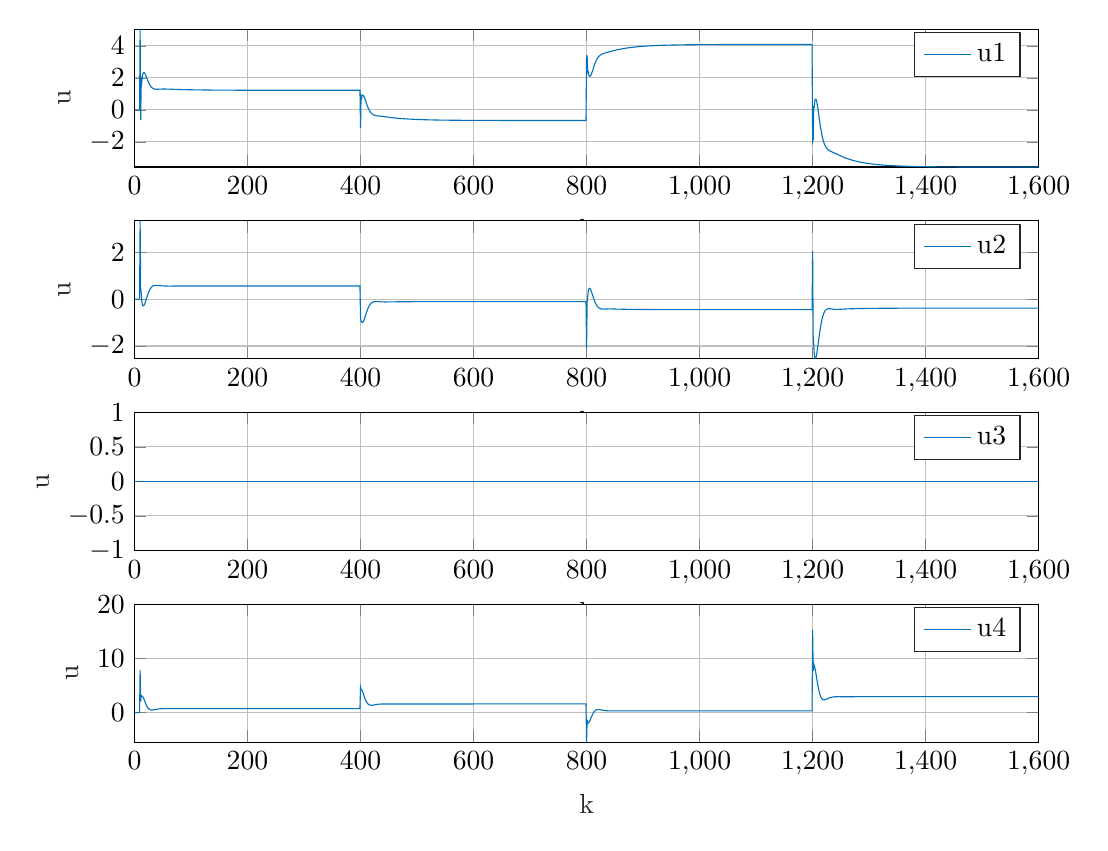
\begin{tikzpicture}

\begin{axis}[%
width=4.521in,
height=0.69in,
at={(0.758in,3.357in)},
scale only axis,
xmin=0,
xmax=1600,
xlabel style={font=\color{white!15!black}},
xlabel={k},
ymin=-3.5671,
ymax=5.0461,
ylabel style={font=\color{white!15!black}},
ylabel={u},
axis background/.style={fill=white},
xmajorgrids,
ymajorgrids,
legend style={legend cell align=left, align=left, draw=white!15!black}
]
\addplot [color=mycolor1]
  table[row sep=crcr]{%
1	0\\
2	0\\
3	0\\
4	0\\
5	0\\
6	0\\
7	0\\
8	0\\
9	0\\
10	5.0461\\
11	-0.63698\\
12	2.0562\\
13	1.756\\
14	2.1578\\
15	2.2499\\
16	2.327\\
17	2.3329\\
18	2.3013\\
19	2.2396\\
20	2.1595\\
21	2.0688\\
22	1.974\\
23	1.88\\
24	1.79\\
25	1.7065\\
26	1.6309\\
27	1.564\\
28	1.5058\\
29	1.4563\\
30	1.415\\
31	1.3811\\
32	1.354\\
33	1.3329\\
34	1.3168\\
35	1.3051\\
36	1.2969\\
37	1.2917\\
38	1.2887\\
39	1.2875\\
40	1.2875\\
41	1.2885\\
42	1.29\\
43	1.2919\\
44	1.2939\\
45	1.2959\\
46	1.2977\\
47	1.2993\\
48	1.3007\\
49	1.3017\\
50	1.3025\\
51	1.3029\\
52	1.303\\
53	1.3029\\
54	1.3026\\
55	1.302\\
56	1.3012\\
57	1.3003\\
58	1.2993\\
59	1.2981\\
60	1.2969\\
61	1.2956\\
62	1.2943\\
63	1.2929\\
64	1.2916\\
65	1.2902\\
66	1.2888\\
67	1.2875\\
68	1.2862\\
69	1.2849\\
70	1.2836\\
71	1.2824\\
72	1.2811\\
73	1.28\\
74	1.2788\\
75	1.2777\\
76	1.2766\\
77	1.2755\\
78	1.2745\\
79	1.2734\\
80	1.2724\\
81	1.2715\\
82	1.2705\\
83	1.2696\\
84	1.2687\\
85	1.2678\\
86	1.2669\\
87	1.266\\
88	1.2652\\
89	1.2643\\
90	1.2635\\
91	1.2627\\
92	1.2619\\
93	1.2612\\
94	1.2604\\
95	1.2597\\
96	1.259\\
97	1.2582\\
98	1.2575\\
99	1.2568\\
100	1.2562\\
101	1.2555\\
102	1.2549\\
103	1.2542\\
104	1.2536\\
105	1.253\\
106	1.2524\\
107	1.2518\\
108	1.2512\\
109	1.2506\\
110	1.2501\\
111	1.2495\\
112	1.249\\
113	1.2485\\
114	1.248\\
115	1.2475\\
116	1.247\\
117	1.2465\\
118	1.246\\
119	1.2455\\
120	1.2451\\
121	1.2446\\
122	1.2442\\
123	1.2438\\
124	1.2433\\
125	1.2429\\
126	1.2425\\
127	1.2421\\
128	1.2417\\
129	1.2413\\
130	1.241\\
131	1.2406\\
132	1.2403\\
133	1.2399\\
134	1.2396\\
135	1.2392\\
136	1.2389\\
137	1.2386\\
138	1.2382\\
139	1.2379\\
140	1.2376\\
141	1.2373\\
142	1.237\\
143	1.2368\\
144	1.2365\\
145	1.2362\\
146	1.2359\\
147	1.2357\\
148	1.2354\\
149	1.2352\\
150	1.2349\\
151	1.2347\\
152	1.2344\\
153	1.2342\\
154	1.234\\
155	1.2338\\
156	1.2335\\
157	1.2333\\
158	1.2331\\
159	1.2329\\
160	1.2327\\
161	1.2325\\
162	1.2323\\
163	1.2321\\
164	1.232\\
165	1.2318\\
166	1.2316\\
167	1.2314\\
168	1.2313\\
169	1.2311\\
170	1.2309\\
171	1.2308\\
172	1.2306\\
173	1.2305\\
174	1.2303\\
175	1.2302\\
176	1.23\\
177	1.2299\\
178	1.2298\\
179	1.2296\\
180	1.2295\\
181	1.2294\\
182	1.2292\\
183	1.2291\\
184	1.229\\
185	1.2289\\
186	1.2288\\
187	1.2287\\
188	1.2285\\
189	1.2284\\
190	1.2283\\
191	1.2282\\
192	1.2281\\
193	1.228\\
194	1.2279\\
195	1.2278\\
196	1.2277\\
197	1.2277\\
198	1.2276\\
199	1.2275\\
200	1.2274\\
201	1.2273\\
202	1.2272\\
203	1.2271\\
204	1.2271\\
205	1.227\\
206	1.2269\\
207	1.2268\\
208	1.2268\\
209	1.2267\\
210	1.2266\\
211	1.2266\\
212	1.2265\\
213	1.2264\\
214	1.2264\\
215	1.2263\\
216	1.2263\\
217	1.2262\\
218	1.2261\\
219	1.2261\\
220	1.226\\
221	1.226\\
222	1.2259\\
223	1.2259\\
224	1.2258\\
225	1.2258\\
226	1.2257\\
227	1.2257\\
228	1.2256\\
229	1.2256\\
230	1.2255\\
231	1.2255\\
232	1.2255\\
233	1.2254\\
234	1.2254\\
235	1.2253\\
236	1.2253\\
237	1.2253\\
238	1.2252\\
239	1.2252\\
240	1.2251\\
241	1.2251\\
242	1.2251\\
243	1.225\\
244	1.225\\
245	1.225\\
246	1.2249\\
247	1.2249\\
248	1.2249\\
249	1.2249\\
250	1.2248\\
251	1.2248\\
252	1.2248\\
253	1.2247\\
254	1.2247\\
255	1.2247\\
256	1.2247\\
257	1.2246\\
258	1.2246\\
259	1.2246\\
260	1.2246\\
261	1.2246\\
262	1.2245\\
263	1.2245\\
264	1.2245\\
265	1.2245\\
266	1.2244\\
267	1.2244\\
268	1.2244\\
269	1.2244\\
270	1.2244\\
271	1.2244\\
272	1.2243\\
273	1.2243\\
274	1.2243\\
275	1.2243\\
276	1.2243\\
277	1.2243\\
278	1.2242\\
279	1.2242\\
280	1.2242\\
281	1.2242\\
282	1.2242\\
283	1.2242\\
284	1.2242\\
285	1.2241\\
286	1.2241\\
287	1.2241\\
288	1.2241\\
289	1.2241\\
290	1.2241\\
291	1.2241\\
292	1.2241\\
293	1.224\\
294	1.224\\
295	1.224\\
296	1.224\\
297	1.224\\
298	1.224\\
299	1.224\\
300	1.224\\
301	1.224\\
302	1.224\\
303	1.2239\\
304	1.2239\\
305	1.2239\\
306	1.2239\\
307	1.2239\\
308	1.2239\\
309	1.2239\\
310	1.2239\\
311	1.2239\\
312	1.2239\\
313	1.2239\\
314	1.2239\\
315	1.2238\\
316	1.2238\\
317	1.2238\\
318	1.2238\\
319	1.2238\\
320	1.2238\\
321	1.2238\\
322	1.2238\\
323	1.2238\\
324	1.2238\\
325	1.2238\\
326	1.2238\\
327	1.2238\\
328	1.2238\\
329	1.2238\\
330	1.2238\\
331	1.2238\\
332	1.2238\\
333	1.2237\\
334	1.2237\\
335	1.2237\\
336	1.2237\\
337	1.2237\\
338	1.2237\\
339	1.2237\\
340	1.2237\\
341	1.2237\\
342	1.2237\\
343	1.2237\\
344	1.2237\\
345	1.2237\\
346	1.2237\\
347	1.2237\\
348	1.2237\\
349	1.2237\\
350	1.2237\\
351	1.2237\\
352	1.2237\\
353	1.2237\\
354	1.2237\\
355	1.2237\\
356	1.2237\\
357	1.2237\\
358	1.2237\\
359	1.2237\\
360	1.2237\\
361	1.2237\\
362	1.2237\\
363	1.2236\\
364	1.2236\\
365	1.2236\\
366	1.2236\\
367	1.2236\\
368	1.2236\\
369	1.2236\\
370	1.2236\\
371	1.2236\\
372	1.2236\\
373	1.2236\\
374	1.2236\\
375	1.2236\\
376	1.2236\\
377	1.2236\\
378	1.2236\\
379	1.2236\\
380	1.2236\\
381	1.2236\\
382	1.2236\\
383	1.2236\\
384	1.2236\\
385	1.2236\\
386	1.2236\\
387	1.2236\\
388	1.2236\\
389	1.2236\\
390	1.2236\\
391	1.2236\\
392	1.2236\\
393	1.2236\\
394	1.2236\\
395	1.2236\\
396	1.2236\\
397	1.2236\\
398	1.2236\\
399	1.2236\\
400	-1.1312\\
401	0.87095\\
402	0.75981\\
403	0.90051\\
404	0.91886\\
405	0.90129\\
406	0.84516\\
407	0.76526\\
408	0.6699\\
409	0.56668\\
410	0.4612\\
411	0.35771\\
412	0.25921\\
413	0.16771\\
414	0.084439\\
415	0.0099625\\
416	-0.055611\\
417	-0.11253\\
418	-0.16129\\
419	-0.20256\\
420	-0.23708\\
421	-0.26565\\
422	-0.28907\\
423	-0.30811\\
424	-0.32349\\
425	-0.33586\\
426	-0.34582\\
427	-0.35389\\
428	-0.3605\\
429	-0.36603\\
430	-0.3708\\
431	-0.37506\\
432	-0.37901\\
433	-0.3828\\
434	-0.38656\\
435	-0.39035\\
436	-0.39424\\
437	-0.39825\\
438	-0.40241\\
439	-0.40672\\
440	-0.41117\\
441	-0.41573\\
442	-0.4204\\
443	-0.42515\\
444	-0.42996\\
445	-0.43481\\
446	-0.43966\\
447	-0.44451\\
448	-0.44933\\
449	-0.45411\\
450	-0.45882\\
451	-0.46347\\
452	-0.46804\\
453	-0.47253\\
454	-0.47692\\
455	-0.48122\\
456	-0.48541\\
457	-0.48951\\
458	-0.49351\\
459	-0.4974\\
460	-0.5012\\
461	-0.5049\\
462	-0.50851\\
463	-0.51202\\
464	-0.51545\\
465	-0.51878\\
466	-0.52204\\
467	-0.52521\\
468	-0.5283\\
469	-0.53131\\
470	-0.53426\\
471	-0.53713\\
472	-0.53993\\
473	-0.54266\\
474	-0.54533\\
475	-0.54794\\
476	-0.55048\\
477	-0.55297\\
478	-0.5554\\
479	-0.55777\\
480	-0.56009\\
481	-0.56235\\
482	-0.56457\\
483	-0.56673\\
484	-0.56884\\
485	-0.5709\\
486	-0.57292\\
487	-0.57489\\
488	-0.57682\\
489	-0.5787\\
490	-0.58054\\
491	-0.58234\\
492	-0.5841\\
493	-0.58581\\
494	-0.58749\\
495	-0.58913\\
496	-0.59073\\
497	-0.5923\\
498	-0.59383\\
499	-0.59533\\
500	-0.59679\\
501	-0.59822\\
502	-0.59962\\
503	-0.60098\\
504	-0.60232\\
505	-0.60362\\
506	-0.60489\\
507	-0.60614\\
508	-0.60736\\
509	-0.60855\\
510	-0.60971\\
511	-0.61085\\
512	-0.61196\\
513	-0.61305\\
514	-0.61411\\
515	-0.61514\\
516	-0.61616\\
517	-0.61715\\
518	-0.61812\\
519	-0.61907\\
520	-0.61999\\
521	-0.6209\\
522	-0.62179\\
523	-0.62265\\
524	-0.6235\\
525	-0.62432\\
526	-0.62513\\
527	-0.62592\\
528	-0.6267\\
529	-0.62745\\
530	-0.62819\\
531	-0.62891\\
532	-0.62962\\
533	-0.63031\\
534	-0.63098\\
535	-0.63164\\
536	-0.63229\\
537	-0.63292\\
538	-0.63354\\
539	-0.63414\\
540	-0.63473\\
541	-0.6353\\
542	-0.63587\\
543	-0.63642\\
544	-0.63696\\
545	-0.63748\\
546	-0.638\\
547	-0.6385\\
548	-0.63899\\
549	-0.63948\\
550	-0.63995\\
551	-0.64041\\
552	-0.64086\\
553	-0.6413\\
554	-0.64173\\
555	-0.64215\\
556	-0.64256\\
557	-0.64296\\
558	-0.64335\\
559	-0.64374\\
560	-0.64412\\
561	-0.64448\\
562	-0.64484\\
563	-0.64519\\
564	-0.64554\\
565	-0.64587\\
566	-0.6462\\
567	-0.64652\\
568	-0.64684\\
569	-0.64715\\
570	-0.64745\\
571	-0.64774\\
572	-0.64803\\
573	-0.64831\\
574	-0.64859\\
575	-0.64885\\
576	-0.64912\\
577	-0.64937\\
578	-0.64963\\
579	-0.64987\\
580	-0.65011\\
581	-0.65035\\
582	-0.65058\\
583	-0.6508\\
584	-0.65102\\
585	-0.65124\\
586	-0.65145\\
587	-0.65165\\
588	-0.65185\\
589	-0.65205\\
590	-0.65224\\
591	-0.65243\\
592	-0.65262\\
593	-0.6528\\
594	-0.65297\\
595	-0.65314\\
596	-0.65331\\
597	-0.65348\\
598	-0.65364\\
599	-0.6538\\
600	-0.65395\\
601	-0.6541\\
602	-0.65425\\
603	-0.65439\\
604	-0.65453\\
605	-0.65467\\
606	-0.6548\\
607	-0.65494\\
608	-0.65507\\
609	-0.65519\\
610	-0.65531\\
611	-0.65544\\
612	-0.65555\\
613	-0.65567\\
614	-0.65578\\
615	-0.65589\\
616	-0.656\\
617	-0.65611\\
618	-0.65621\\
619	-0.65631\\
620	-0.65641\\
621	-0.6565\\
622	-0.6566\\
623	-0.65669\\
624	-0.65678\\
625	-0.65687\\
626	-0.65696\\
627	-0.65704\\
628	-0.65712\\
629	-0.6572\\
630	-0.65728\\
631	-0.65736\\
632	-0.65744\\
633	-0.65751\\
634	-0.65758\\
635	-0.65765\\
636	-0.65772\\
637	-0.65779\\
638	-0.65786\\
639	-0.65792\\
640	-0.65799\\
641	-0.65805\\
642	-0.65811\\
643	-0.65817\\
644	-0.65823\\
645	-0.65828\\
646	-0.65834\\
647	-0.65839\\
648	-0.65844\\
649	-0.6585\\
650	-0.65855\\
651	-0.6586\\
652	-0.65865\\
653	-0.65869\\
654	-0.65874\\
655	-0.65878\\
656	-0.65883\\
657	-0.65887\\
658	-0.65892\\
659	-0.65896\\
660	-0.659\\
661	-0.65904\\
662	-0.65908\\
663	-0.65911\\
664	-0.65915\\
665	-0.65919\\
666	-0.65922\\
667	-0.65926\\
668	-0.65929\\
669	-0.65933\\
670	-0.65936\\
671	-0.65939\\
672	-0.65942\\
673	-0.65945\\
674	-0.65948\\
675	-0.65951\\
676	-0.65954\\
677	-0.65957\\
678	-0.65959\\
679	-0.65962\\
680	-0.65965\\
681	-0.65967\\
682	-0.6597\\
683	-0.65972\\
684	-0.65975\\
685	-0.65977\\
686	-0.65979\\
687	-0.65982\\
688	-0.65984\\
689	-0.65986\\
690	-0.65988\\
691	-0.6599\\
692	-0.65992\\
693	-0.65994\\
694	-0.65996\\
695	-0.65998\\
696	-0.66\\
697	-0.66001\\
698	-0.66003\\
699	-0.66005\\
700	-0.66007\\
701	-0.66008\\
702	-0.6601\\
703	-0.66011\\
704	-0.66013\\
705	-0.66014\\
706	-0.66016\\
707	-0.66017\\
708	-0.66019\\
709	-0.6602\\
710	-0.66021\\
711	-0.66023\\
712	-0.66024\\
713	-0.66025\\
714	-0.66026\\
715	-0.66028\\
716	-0.66029\\
717	-0.6603\\
718	-0.66031\\
719	-0.66032\\
720	-0.66033\\
721	-0.66034\\
722	-0.66035\\
723	-0.66036\\
724	-0.66037\\
725	-0.66038\\
726	-0.66039\\
727	-0.6604\\
728	-0.66041\\
729	-0.66042\\
730	-0.66043\\
731	-0.66044\\
732	-0.66045\\
733	-0.66045\\
734	-0.66046\\
735	-0.66047\\
736	-0.66048\\
737	-0.66048\\
738	-0.66049\\
739	-0.6605\\
740	-0.66051\\
741	-0.66051\\
742	-0.66052\\
743	-0.66053\\
744	-0.66053\\
745	-0.66054\\
746	-0.66054\\
747	-0.66055\\
748	-0.66056\\
749	-0.66056\\
750	-0.66057\\
751	-0.66057\\
752	-0.66058\\
753	-0.66058\\
754	-0.66059\\
755	-0.66059\\
756	-0.6606\\
757	-0.6606\\
758	-0.66061\\
759	-0.66061\\
760	-0.66062\\
761	-0.66062\\
762	-0.66063\\
763	-0.66063\\
764	-0.66063\\
765	-0.66064\\
766	-0.66064\\
767	-0.66064\\
768	-0.66065\\
769	-0.66065\\
770	-0.66066\\
771	-0.66066\\
772	-0.66066\\
773	-0.66067\\
774	-0.66067\\
775	-0.66067\\
776	-0.66068\\
777	-0.66068\\
778	-0.66068\\
779	-0.66068\\
780	-0.66069\\
781	-0.66069\\
782	-0.66069\\
783	-0.6607\\
784	-0.6607\\
785	-0.6607\\
786	-0.6607\\
787	-0.66071\\
788	-0.66071\\
789	-0.66071\\
790	-0.66071\\
791	-0.66072\\
792	-0.66072\\
793	-0.66072\\
794	-0.66072\\
795	-0.66072\\
796	-0.66073\\
797	-0.66073\\
798	-0.66073\\
799	-0.66073\\
800	3.3761\\
801	3.3735\\
802	2.34\\
803	2.374\\
804	2.1598\\
805	2.1117\\
806	2.0953\\
807	2.1301\\
808	2.1956\\
809	2.2837\\
810	2.3853\\
811	2.4937\\
812	2.6036\\
813	2.7112\\
814	2.8136\\
815	2.909\\
816	2.9963\\
817	3.075\\
818	3.1452\\
819	3.2069\\
820	3.2609\\
821	3.3076\\
822	3.3478\\
823	3.3823\\
824	3.4118\\
825	3.4371\\
826	3.4589\\
827	3.4777\\
828	3.4942\\
829	3.5087\\
830	3.5218\\
831	3.5337\\
832	3.5448\\
833	3.5553\\
834	3.5653\\
835	3.5751\\
836	3.5847\\
837	3.5942\\
838	3.6036\\
839	3.6131\\
840	3.6225\\
841	3.6319\\
842	3.6413\\
843	3.6507\\
844	3.6601\\
845	3.6694\\
846	3.6786\\
847	3.6878\\
848	3.6968\\
849	3.7057\\
850	3.7145\\
851	3.7231\\
852	3.7316\\
853	3.7398\\
854	3.748\\
855	3.7559\\
856	3.7637\\
857	3.7712\\
858	3.7786\\
859	3.7858\\
860	3.7928\\
861	3.7997\\
862	3.8064\\
863	3.8129\\
864	3.8192\\
865	3.8254\\
866	3.8314\\
867	3.8373\\
868	3.843\\
869	3.8486\\
870	3.8541\\
871	3.8594\\
872	3.8646\\
873	3.8697\\
874	3.8746\\
875	3.8794\\
876	3.8841\\
877	3.8887\\
878	3.8932\\
879	3.8976\\
880	3.9018\\
881	3.906\\
882	3.9101\\
883	3.9141\\
884	3.9179\\
885	3.9217\\
886	3.9254\\
887	3.9291\\
888	3.9326\\
889	3.9361\\
890	3.9394\\
891	3.9427\\
892	3.9459\\
893	3.9491\\
894	3.9522\\
895	3.9551\\
896	3.9581\\
897	3.9609\\
898	3.9637\\
899	3.9665\\
900	3.9691\\
901	3.9717\\
902	3.9743\\
903	3.9768\\
904	3.9792\\
905	3.9816\\
906	3.9839\\
907	3.9862\\
908	3.9884\\
909	3.9905\\
910	3.9927\\
911	3.9947\\
912	3.9967\\
913	3.9987\\
914	4.0006\\
915	4.0025\\
916	4.0044\\
917	4.0062\\
918	4.0079\\
919	4.0096\\
920	4.0113\\
921	4.013\\
922	4.0146\\
923	4.0161\\
924	4.0177\\
925	4.0192\\
926	4.0206\\
927	4.022\\
928	4.0234\\
929	4.0248\\
930	4.0261\\
931	4.0274\\
932	4.0287\\
933	4.03\\
934	4.0312\\
935	4.0324\\
936	4.0335\\
937	4.0347\\
938	4.0358\\
939	4.0369\\
940	4.0379\\
941	4.039\\
942	4.04\\
943	4.041\\
944	4.042\\
945	4.0429\\
946	4.0438\\
947	4.0447\\
948	4.0456\\
949	4.0465\\
950	4.0473\\
951	4.0482\\
952	4.049\\
953	4.0498\\
954	4.0505\\
955	4.0513\\
956	4.052\\
957	4.0527\\
958	4.0535\\
959	4.0541\\
960	4.0548\\
961	4.0555\\
962	4.0561\\
963	4.0568\\
964	4.0574\\
965	4.058\\
966	4.0586\\
967	4.0591\\
968	4.0597\\
969	4.0603\\
970	4.0608\\
971	4.0613\\
972	4.0618\\
973	4.0623\\
974	4.0628\\
975	4.0633\\
976	4.0638\\
977	4.0642\\
978	4.0647\\
979	4.0651\\
980	4.0656\\
981	4.066\\
982	4.0664\\
983	4.0668\\
984	4.0672\\
985	4.0676\\
986	4.068\\
987	4.0683\\
988	4.0687\\
989	4.069\\
990	4.0694\\
991	4.0697\\
992	4.07\\
993	4.0704\\
994	4.0707\\
995	4.071\\
996	4.0713\\
997	4.0716\\
998	4.0719\\
999	4.0722\\
1000	4.0724\\
1001	4.0727\\
1002	4.073\\
1003	4.0732\\
1004	4.0735\\
1005	4.0737\\
1006	4.074\\
1007	4.0742\\
1008	4.0744\\
1009	4.0746\\
1010	4.0749\\
1011	4.0751\\
1012	4.0753\\
1013	4.0755\\
1014	4.0757\\
1015	4.0759\\
1016	4.0761\\
1017	4.0763\\
1018	4.0765\\
1019	4.0766\\
1020	4.0768\\
1021	4.077\\
1022	4.0772\\
1023	4.0773\\
1024	4.0775\\
1025	4.0776\\
1026	4.0778\\
1027	4.0779\\
1028	4.0781\\
1029	4.0782\\
1030	4.0784\\
1031	4.0785\\
1032	4.0787\\
1033	4.0788\\
1034	4.0789\\
1035	4.079\\
1036	4.0792\\
1037	4.0793\\
1038	4.0794\\
1039	4.0795\\
1040	4.0796\\
1041	4.0797\\
1042	4.0798\\
1043	4.08\\
1044	4.0801\\
1045	4.0802\\
1046	4.0803\\
1047	4.0804\\
1048	4.0804\\
1049	4.0805\\
1050	4.0806\\
1051	4.0807\\
1052	4.0808\\
1053	4.0809\\
1054	4.081\\
1055	4.0811\\
1056	4.0811\\
1057	4.0812\\
1058	4.0813\\
1059	4.0814\\
1060	4.0814\\
1061	4.0815\\
1062	4.0816\\
1063	4.0816\\
1064	4.0817\\
1065	4.0818\\
1066	4.0818\\
1067	4.0819\\
1068	4.082\\
1069	4.082\\
1070	4.0821\\
1071	4.0821\\
1072	4.0822\\
1073	4.0822\\
1074	4.0823\\
1075	4.0823\\
1076	4.0824\\
1077	4.0824\\
1078	4.0825\\
1079	4.0825\\
1080	4.0826\\
1081	4.0826\\
1082	4.0827\\
1083	4.0827\\
1084	4.0828\\
1085	4.0828\\
1086	4.0828\\
1087	4.0829\\
1088	4.0829\\
1089	4.083\\
1090	4.083\\
1091	4.083\\
1092	4.0831\\
1093	4.0831\\
1094	4.0831\\
1095	4.0832\\
1096	4.0832\\
1097	4.0832\\
1098	4.0833\\
1099	4.0833\\
1100	4.0833\\
1101	4.0834\\
1102	4.0834\\
1103	4.0834\\
1104	4.0834\\
1105	4.0835\\
1106	4.0835\\
1107	4.0835\\
1108	4.0835\\
1109	4.0836\\
1110	4.0836\\
1111	4.0836\\
1112	4.0836\\
1113	4.0837\\
1114	4.0837\\
1115	4.0837\\
1116	4.0837\\
1117	4.0838\\
1118	4.0838\\
1119	4.0838\\
1120	4.0838\\
1121	4.0838\\
1122	4.0838\\
1123	4.0839\\
1124	4.0839\\
1125	4.0839\\
1126	4.0839\\
1127	4.0839\\
1128	4.0839\\
1129	4.084\\
1130	4.084\\
1131	4.084\\
1132	4.084\\
1133	4.084\\
1134	4.084\\
1135	4.0841\\
1136	4.0841\\
1137	4.0841\\
1138	4.0841\\
1139	4.0841\\
1140	4.0841\\
1141	4.0841\\
1142	4.0841\\
1143	4.0842\\
1144	4.0842\\
1145	4.0842\\
1146	4.0842\\
1147	4.0842\\
1148	4.0842\\
1149	4.0842\\
1150	4.0842\\
1151	4.0842\\
1152	4.0842\\
1153	4.0843\\
1154	4.0843\\
1155	4.0843\\
1156	4.0843\\
1157	4.0843\\
1158	4.0843\\
1159	4.0843\\
1160	4.0843\\
1161	4.0843\\
1162	4.0843\\
1163	4.0843\\
1164	4.0843\\
1165	4.0843\\
1166	4.0844\\
1167	4.0844\\
1168	4.0844\\
1169	4.0844\\
1170	4.0844\\
1171	4.0844\\
1172	4.0844\\
1173	4.0844\\
1174	4.0844\\
1175	4.0844\\
1176	4.0844\\
1177	4.0844\\
1178	4.0844\\
1179	4.0844\\
1180	4.0844\\
1181	4.0844\\
1182	4.0844\\
1183	4.0845\\
1184	4.0845\\
1185	4.0845\\
1186	4.0845\\
1187	4.0845\\
1188	4.0845\\
1189	4.0845\\
1190	4.0845\\
1191	4.0845\\
1192	4.0845\\
1193	4.0845\\
1194	4.0845\\
1195	4.0845\\
1196	4.0845\\
1197	4.0845\\
1198	4.0845\\
1199	4.0845\\
1200	-1.9707\\
1201	-1.8383\\
1202	0.1919\\
1203	0.1815\\
1204	0.59449\\
1205	0.66984\\
1206	0.66633\\
1207	0.5548\\
1208	0.37885\\
1209	0.15773\\
1210	-0.088486\\
1211	-0.34513\\
1212	-0.60079\\
1213	-0.84725\\
1214	-1.0788\\
1215	-1.2919\\
1216	-1.4846\\
1217	-1.6563\\
1218	-1.8071\\
1219	-1.9381\\
1220	-2.0507\\
1221	-2.1466\\
1222	-2.2277\\
1223	-2.2958\\
1224	-2.3528\\
1225	-2.4005\\
1226	-2.4404\\
1227	-2.4739\\
1228	-2.5024\\
1229	-2.527\\
1230	-2.5487\\
1231	-2.5681\\
1232	-2.5859\\
1233	-2.6027\\
1234	-2.6189\\
1235	-2.6347\\
1236	-2.6504\\
1237	-2.6662\\
1238	-2.682\\
1239	-2.6981\\
1240	-2.7143\\
1241	-2.7307\\
1242	-2.7473\\
1243	-2.7639\\
1244	-2.7807\\
1245	-2.7974\\
1246	-2.8142\\
1247	-2.8308\\
1248	-2.8473\\
1249	-2.8636\\
1250	-2.8797\\
1251	-2.8955\\
1252	-2.9111\\
1253	-2.9264\\
1254	-2.9414\\
1255	-2.956\\
1256	-2.9704\\
1257	-2.9844\\
1258	-2.998\\
1259	-3.0113\\
1260	-3.0243\\
1261	-3.037\\
1262	-3.0493\\
1263	-3.0614\\
1264	-3.0731\\
1265	-3.0845\\
1266	-3.0957\\
1267	-3.1065\\
1268	-3.1171\\
1269	-3.1275\\
1270	-3.1376\\
1271	-3.1474\\
1272	-3.157\\
1273	-3.1663\\
1274	-3.1755\\
1275	-3.1844\\
1276	-3.1931\\
1277	-3.2016\\
1278	-3.2099\\
1279	-3.218\\
1280	-3.2259\\
1281	-3.2337\\
1282	-3.2412\\
1283	-3.2486\\
1284	-3.2558\\
1285	-3.2628\\
1286	-3.2697\\
1287	-3.2764\\
1288	-3.283\\
1289	-3.2894\\
1290	-3.2957\\
1291	-3.3018\\
1292	-3.3078\\
1293	-3.3136\\
1294	-3.3193\\
1295	-3.3249\\
1296	-3.3304\\
1297	-3.3357\\
1298	-3.3409\\
1299	-3.346\\
1300	-3.351\\
1301	-3.3558\\
1302	-3.3606\\
1303	-3.3652\\
1304	-3.3697\\
1305	-3.3742\\
1306	-3.3785\\
1307	-3.3827\\
1308	-3.3868\\
1309	-3.3909\\
1310	-3.3948\\
1311	-3.3987\\
1312	-3.4024\\
1313	-3.4061\\
1314	-3.4097\\
1315	-3.4132\\
1316	-3.4167\\
1317	-3.42\\
1318	-3.4233\\
1319	-3.4265\\
1320	-3.4297\\
1321	-3.4327\\
1322	-3.4357\\
1323	-3.4387\\
1324	-3.4415\\
1325	-3.4443\\
1326	-3.4471\\
1327	-3.4497\\
1328	-3.4524\\
1329	-3.4549\\
1330	-3.4574\\
1331	-3.4599\\
1332	-3.4622\\
1333	-3.4646\\
1334	-3.4669\\
1335	-3.4691\\
1336	-3.4713\\
1337	-3.4734\\
1338	-3.4755\\
1339	-3.4775\\
1340	-3.4795\\
1341	-3.4815\\
1342	-3.4834\\
1343	-3.4852\\
1344	-3.487\\
1345	-3.4888\\
1346	-3.4905\\
1347	-3.4922\\
1348	-3.4939\\
1349	-3.4955\\
1350	-3.4971\\
1351	-3.4987\\
1352	-3.5002\\
1353	-3.5017\\
1354	-3.5031\\
1355	-3.5045\\
1356	-3.5059\\
1357	-3.5073\\
1358	-3.5086\\
1359	-3.5099\\
1360	-3.5112\\
1361	-3.5124\\
1362	-3.5136\\
1363	-3.5148\\
1364	-3.516\\
1365	-3.5171\\
1366	-3.5182\\
1367	-3.5193\\
1368	-3.5204\\
1369	-3.5214\\
1370	-3.5224\\
1371	-3.5234\\
1372	-3.5244\\
1373	-3.5253\\
1374	-3.5262\\
1375	-3.5272\\
1376	-3.528\\
1377	-3.5289\\
1378	-3.5297\\
1379	-3.5306\\
1380	-3.5314\\
1381	-3.5322\\
1382	-3.533\\
1383	-3.5337\\
1384	-3.5345\\
1385	-3.5352\\
1386	-3.5359\\
1387	-3.5366\\
1388	-3.5373\\
1389	-3.5379\\
1390	-3.5386\\
1391	-3.5392\\
1392	-3.5398\\
1393	-3.5404\\
1394	-3.541\\
1395	-3.5416\\
1396	-3.5422\\
1397	-3.5427\\
1398	-3.5433\\
1399	-3.5438\\
1400	-3.5443\\
1401	-3.5448\\
1402	-3.5453\\
1403	-3.5458\\
1404	-3.5463\\
1405	-3.5467\\
1406	-3.5472\\
1407	-3.5476\\
1408	-3.5481\\
1409	-3.5485\\
1410	-3.5489\\
1411	-3.5493\\
1412	-3.5497\\
1413	-3.5501\\
1414	-3.5505\\
1415	-3.5508\\
1416	-3.5512\\
1417	-3.5516\\
1418	-3.5519\\
1419	-3.5522\\
1420	-3.5526\\
1421	-3.5529\\
1422	-3.5532\\
1423	-3.5535\\
1424	-3.5538\\
1425	-3.5541\\
1426	-3.5544\\
1427	-3.5547\\
1428	-3.555\\
1429	-3.5552\\
1430	-3.5555\\
1431	-3.5558\\
1432	-3.556\\
1433	-3.5563\\
1434	-3.5565\\
1435	-3.5568\\
1436	-3.557\\
1437	-3.5572\\
1438	-3.5574\\
1439	-3.5577\\
1440	-3.5579\\
1441	-3.5581\\
1442	-3.5583\\
1443	-3.5585\\
1444	-3.5587\\
1445	-3.5589\\
1446	-3.5591\\
1447	-3.5592\\
1448	-3.5594\\
1449	-3.5596\\
1450	-3.5598\\
1451	-3.5599\\
1452	-3.5601\\
1453	-3.5602\\
1454	-3.5604\\
1455	-3.5606\\
1456	-3.5607\\
1457	-3.5609\\
1458	-3.561\\
1459	-3.5611\\
1460	-3.5613\\
1461	-3.5614\\
1462	-3.5615\\
1463	-3.5617\\
1464	-3.5618\\
1465	-3.5619\\
1466	-3.562\\
1467	-3.5621\\
1468	-3.5623\\
1469	-3.5624\\
1470	-3.5625\\
1471	-3.5626\\
1472	-3.5627\\
1473	-3.5628\\
1474	-3.5629\\
1475	-3.563\\
1476	-3.5631\\
1477	-3.5632\\
1478	-3.5633\\
1479	-3.5634\\
1480	-3.5635\\
1481	-3.5635\\
1482	-3.5636\\
1483	-3.5637\\
1484	-3.5638\\
1485	-3.5639\\
1486	-3.5639\\
1487	-3.564\\
1488	-3.5641\\
1489	-3.5642\\
1490	-3.5642\\
1491	-3.5643\\
1492	-3.5644\\
1493	-3.5644\\
1494	-3.5645\\
1495	-3.5646\\
1496	-3.5646\\
1497	-3.5647\\
1498	-3.5647\\
1499	-3.5648\\
1500	-3.5649\\
1501	-3.5649\\
1502	-3.565\\
1503	-3.565\\
1504	-3.5651\\
1505	-3.5651\\
1506	-3.5652\\
1507	-3.5652\\
1508	-3.5653\\
1509	-3.5653\\
1510	-3.5654\\
1511	-3.5654\\
1512	-3.5654\\
1513	-3.5655\\
1514	-3.5655\\
1515	-3.5656\\
1516	-3.5656\\
1517	-3.5656\\
1518	-3.5657\\
1519	-3.5657\\
1520	-3.5658\\
1521	-3.5658\\
1522	-3.5658\\
1523	-3.5659\\
1524	-3.5659\\
1525	-3.5659\\
1526	-3.566\\
1527	-3.566\\
1528	-3.566\\
1529	-3.566\\
1530	-3.5661\\
1531	-3.5661\\
1532	-3.5661\\
1533	-3.5662\\
1534	-3.5662\\
1535	-3.5662\\
1536	-3.5662\\
1537	-3.5663\\
1538	-3.5663\\
1539	-3.5663\\
1540	-3.5663\\
1541	-3.5664\\
1542	-3.5664\\
1543	-3.5664\\
1544	-3.5664\\
1545	-3.5664\\
1546	-3.5665\\
1547	-3.5665\\
1548	-3.5665\\
1549	-3.5665\\
1550	-3.5665\\
1551	-3.5666\\
1552	-3.5666\\
1553	-3.5666\\
1554	-3.5666\\
1555	-3.5666\\
1556	-3.5666\\
1557	-3.5667\\
1558	-3.5667\\
1559	-3.5667\\
1560	-3.5667\\
1561	-3.5667\\
1562	-3.5667\\
1563	-3.5667\\
1564	-3.5668\\
1565	-3.5668\\
1566	-3.5668\\
1567	-3.5668\\
1568	-3.5668\\
1569	-3.5668\\
1570	-3.5668\\
1571	-3.5668\\
1572	-3.5669\\
1573	-3.5669\\
1574	-3.5669\\
1575	-3.5669\\
1576	-3.5669\\
1577	-3.5669\\
1578	-3.5669\\
1579	-3.5669\\
1580	-3.5669\\
1581	-3.567\\
1582	-3.567\\
1583	-3.567\\
1584	-3.567\\
1585	-3.567\\
1586	-3.567\\
1587	-3.567\\
1588	-3.567\\
1589	-3.567\\
1590	-3.567\\
1591	-3.567\\
1592	-3.567\\
1593	-3.567\\
1594	-3.5671\\
1595	-3.5671\\
1596	-3.5671\\
1597	-3.5671\\
1598	-3.5671\\
1599	-3.5671\\
1600	-3.5671\\
};
\addlegendentry{u1}

\end{axis}

\begin{axis}[%
width=4.521in,
height=0.69in,
at={(0.758in,2.398in)},
scale only axis,
xmin=0,
xmax=1600,
xlabel style={font=\color{white!15!black}},
xlabel={k},
ymin=-2.5501,
ymax=3.3383,
ylabel style={font=\color{white!15!black}},
ylabel={u},
axis background/.style={fill=white},
xmajorgrids,
ymajorgrids,
legend style={legend cell align=left, align=left, draw=white!15!black}
]
\addplot [color=mycolor1]
  table[row sep=crcr]{%
1	0\\
2	0\\
3	0\\
4	0\\
5	0\\
6	0\\
7	0\\
8	0\\
9	0\\
10	3.3383\\
11	0.46197\\
12	0.23069\\
13	-0.11284\\
14	-0.22696\\
15	-0.28704\\
16	-0.2916\\
17	-0.26365\\
18	-0.21227\\
19	-0.14621\\
20	-0.071753\\
21	0.0061176\\
22	0.083671\\
23	0.15817\\
24	0.22773\\
25	0.29113\\
26	0.3477\\
27	0.39718\\
28	0.43964\\
29	0.47539\\
30	0.50489\\
31	0.5287\\
32	0.54745\\
33	0.56178\\
34	0.57231\\
35	0.57965\\
36	0.58436\\
37	0.58695\\
38	0.58785\\
39	0.58748\\
40	0.58617\\
41	0.5842\\
42	0.58181\\
43	0.57918\\
44	0.57647\\
45	0.57378\\
46	0.57121\\
47	0.56881\\
48	0.56661\\
49	0.56464\\
50	0.56291\\
51	0.56142\\
52	0.56014\\
53	0.55908\\
54	0.55821\\
55	0.55751\\
56	0.55696\\
57	0.55654\\
58	0.55623\\
59	0.55601\\
60	0.55587\\
61	0.55579\\
62	0.55575\\
63	0.55575\\
64	0.55578\\
65	0.55582\\
66	0.55587\\
67	0.55593\\
68	0.556\\
69	0.55606\\
70	0.55612\\
71	0.55617\\
72	0.55622\\
73	0.55627\\
74	0.5563\\
75	0.55634\\
76	0.55636\\
77	0.55639\\
78	0.5564\\
79	0.55642\\
80	0.55643\\
81	0.55644\\
82	0.55644\\
83	0.55645\\
84	0.55645\\
85	0.55645\\
86	0.55646\\
87	0.55646\\
88	0.55646\\
89	0.55647\\
90	0.55647\\
91	0.55647\\
92	0.55648\\
93	0.55648\\
94	0.55649\\
95	0.55649\\
96	0.5565\\
97	0.55651\\
98	0.55652\\
99	0.55653\\
100	0.55653\\
101	0.55654\\
102	0.55655\\
103	0.55656\\
104	0.55657\\
105	0.55659\\
106	0.5566\\
107	0.55661\\
108	0.55662\\
109	0.55663\\
110	0.55664\\
111	0.55665\\
112	0.55667\\
113	0.55668\\
114	0.55669\\
115	0.5567\\
116	0.55671\\
117	0.55673\\
118	0.55674\\
119	0.55675\\
120	0.55676\\
121	0.55677\\
122	0.55679\\
123	0.5568\\
124	0.55681\\
125	0.55682\\
126	0.55683\\
127	0.55684\\
128	0.55685\\
129	0.55687\\
130	0.55688\\
131	0.55689\\
132	0.5569\\
133	0.55691\\
134	0.55692\\
135	0.55693\\
136	0.55694\\
137	0.55695\\
138	0.55696\\
139	0.55697\\
140	0.55698\\
141	0.55699\\
142	0.557\\
143	0.55701\\
144	0.55702\\
145	0.55703\\
146	0.55704\\
147	0.55705\\
148	0.55706\\
149	0.55707\\
150	0.55708\\
151	0.55709\\
152	0.5571\\
153	0.5571\\
154	0.55711\\
155	0.55712\\
156	0.55713\\
157	0.55714\\
158	0.55715\\
159	0.55715\\
160	0.55716\\
161	0.55717\\
162	0.55718\\
163	0.55718\\
164	0.55719\\
165	0.5572\\
166	0.5572\\
167	0.55721\\
168	0.55722\\
169	0.55722\\
170	0.55723\\
171	0.55724\\
172	0.55724\\
173	0.55725\\
174	0.55726\\
175	0.55726\\
176	0.55727\\
177	0.55727\\
178	0.55728\\
179	0.55729\\
180	0.55729\\
181	0.5573\\
182	0.5573\\
183	0.55731\\
184	0.55731\\
185	0.55732\\
186	0.55732\\
187	0.55733\\
188	0.55733\\
189	0.55734\\
190	0.55734\\
191	0.55734\\
192	0.55735\\
193	0.55735\\
194	0.55736\\
195	0.55736\\
196	0.55737\\
197	0.55737\\
198	0.55737\\
199	0.55738\\
200	0.55738\\
201	0.55739\\
202	0.55739\\
203	0.55739\\
204	0.5574\\
205	0.5574\\
206	0.5574\\
207	0.55741\\
208	0.55741\\
209	0.55741\\
210	0.55742\\
211	0.55742\\
212	0.55742\\
213	0.55742\\
214	0.55743\\
215	0.55743\\
216	0.55743\\
217	0.55744\\
218	0.55744\\
219	0.55744\\
220	0.55744\\
221	0.55745\\
222	0.55745\\
223	0.55745\\
224	0.55745\\
225	0.55746\\
226	0.55746\\
227	0.55746\\
228	0.55746\\
229	0.55746\\
230	0.55747\\
231	0.55747\\
232	0.55747\\
233	0.55747\\
234	0.55747\\
235	0.55748\\
236	0.55748\\
237	0.55748\\
238	0.55748\\
239	0.55748\\
240	0.55748\\
241	0.55749\\
242	0.55749\\
243	0.55749\\
244	0.55749\\
245	0.55749\\
246	0.55749\\
247	0.5575\\
248	0.5575\\
249	0.5575\\
250	0.5575\\
251	0.5575\\
252	0.5575\\
253	0.5575\\
254	0.55751\\
255	0.55751\\
256	0.55751\\
257	0.55751\\
258	0.55751\\
259	0.55751\\
260	0.55751\\
261	0.55751\\
262	0.55751\\
263	0.55752\\
264	0.55752\\
265	0.55752\\
266	0.55752\\
267	0.55752\\
268	0.55752\\
269	0.55752\\
270	0.55752\\
271	0.55752\\
272	0.55752\\
273	0.55752\\
274	0.55753\\
275	0.55753\\
276	0.55753\\
277	0.55753\\
278	0.55753\\
279	0.55753\\
280	0.55753\\
281	0.55753\\
282	0.55753\\
283	0.55753\\
284	0.55753\\
285	0.55753\\
286	0.55753\\
287	0.55753\\
288	0.55754\\
289	0.55754\\
290	0.55754\\
291	0.55754\\
292	0.55754\\
293	0.55754\\
294	0.55754\\
295	0.55754\\
296	0.55754\\
297	0.55754\\
298	0.55754\\
299	0.55754\\
300	0.55754\\
301	0.55754\\
302	0.55754\\
303	0.55754\\
304	0.55754\\
305	0.55754\\
306	0.55754\\
307	0.55754\\
308	0.55755\\
309	0.55755\\
310	0.55755\\
311	0.55755\\
312	0.55755\\
313	0.55755\\
314	0.55755\\
315	0.55755\\
316	0.55755\\
317	0.55755\\
318	0.55755\\
319	0.55755\\
320	0.55755\\
321	0.55755\\
322	0.55755\\
323	0.55755\\
324	0.55755\\
325	0.55755\\
326	0.55755\\
327	0.55755\\
328	0.55755\\
329	0.55755\\
330	0.55755\\
331	0.55755\\
332	0.55755\\
333	0.55755\\
334	0.55755\\
335	0.55755\\
336	0.55755\\
337	0.55755\\
338	0.55755\\
339	0.55755\\
340	0.55755\\
341	0.55755\\
342	0.55755\\
343	0.55755\\
344	0.55756\\
345	0.55756\\
346	0.55756\\
347	0.55756\\
348	0.55756\\
349	0.55756\\
350	0.55756\\
351	0.55756\\
352	0.55756\\
353	0.55756\\
354	0.55756\\
355	0.55756\\
356	0.55756\\
357	0.55756\\
358	0.55756\\
359	0.55756\\
360	0.55756\\
361	0.55756\\
362	0.55756\\
363	0.55756\\
364	0.55756\\
365	0.55756\\
366	0.55756\\
367	0.55756\\
368	0.55756\\
369	0.55756\\
370	0.55756\\
371	0.55756\\
372	0.55756\\
373	0.55756\\
374	0.55756\\
375	0.55756\\
376	0.55756\\
377	0.55756\\
378	0.55756\\
379	0.55756\\
380	0.55756\\
381	0.55756\\
382	0.55756\\
383	0.55756\\
384	0.55756\\
385	0.55756\\
386	0.55756\\
387	0.55756\\
388	0.55756\\
389	0.55756\\
390	0.55756\\
391	0.55756\\
392	0.55756\\
393	0.55756\\
394	0.55756\\
395	0.55756\\
396	0.55756\\
397	0.55756\\
398	0.55756\\
399	0.55756\\
400	-0.77775\\
401	-0.9368\\
402	-0.9765\\
403	-1.0001\\
404	-0.99344\\
405	-0.95952\\
406	-0.90618\\
407	-0.83979\\
408	-0.76605\\
409	-0.68942\\
410	-0.61333\\
411	-0.5403\\
412	-0.47209\\
413	-0.40982\\
414	-0.35412\\
415	-0.3052\\
416	-0.26301\\
417	-0.22725\\
418	-0.19749\\
419	-0.17319\\
420	-0.15376\\
421	-0.13859\\
422	-0.12709\\
423	-0.1187\\
424	-0.11287\\
425	-0.10912\\
426	-0.10703\\
427	-0.10621\\
428	-0.10636\\
429	-0.10718\\
430	-0.10846\\
431	-0.11002\\
432	-0.11171\\
433	-0.11342\\
434	-0.11507\\
435	-0.11659\\
436	-0.11795\\
437	-0.11914\\
438	-0.12013\\
439	-0.12092\\
440	-0.12154\\
441	-0.12198\\
442	-0.12226\\
443	-0.1224\\
444	-0.12242\\
445	-0.12234\\
446	-0.12217\\
447	-0.12193\\
448	-0.12164\\
449	-0.1213\\
450	-0.12094\\
451	-0.12056\\
452	-0.12016\\
453	-0.11977\\
454	-0.11937\\
455	-0.11898\\
456	-0.1186\\
457	-0.11823\\
458	-0.11787\\
459	-0.11753\\
460	-0.1172\\
461	-0.11689\\
462	-0.11659\\
463	-0.11631\\
464	-0.11604\\
465	-0.11578\\
466	-0.11553\\
467	-0.1153\\
468	-0.11507\\
469	-0.11486\\
470	-0.11465\\
471	-0.11445\\
472	-0.11426\\
473	-0.11408\\
474	-0.1139\\
475	-0.11373\\
476	-0.11356\\
477	-0.1134\\
478	-0.11324\\
479	-0.11309\\
480	-0.11294\\
481	-0.1128\\
482	-0.11265\\
483	-0.11252\\
484	-0.11238\\
485	-0.11225\\
486	-0.11212\\
487	-0.112\\
488	-0.11188\\
489	-0.11176\\
490	-0.11165\\
491	-0.11153\\
492	-0.11143\\
493	-0.11132\\
494	-0.11122\\
495	-0.11111\\
496	-0.11102\\
497	-0.11092\\
498	-0.11083\\
499	-0.11073\\
500	-0.11065\\
501	-0.11056\\
502	-0.11047\\
503	-0.11039\\
504	-0.11031\\
505	-0.11023\\
506	-0.11016\\
507	-0.11008\\
508	-0.11001\\
509	-0.10994\\
510	-0.10987\\
511	-0.1098\\
512	-0.10974\\
513	-0.10967\\
514	-0.10961\\
515	-0.10955\\
516	-0.10949\\
517	-0.10943\\
518	-0.10938\\
519	-0.10932\\
520	-0.10927\\
521	-0.10922\\
522	-0.10917\\
523	-0.10912\\
524	-0.10907\\
525	-0.10902\\
526	-0.10897\\
527	-0.10893\\
528	-0.10888\\
529	-0.10884\\
530	-0.1088\\
531	-0.10876\\
532	-0.10872\\
533	-0.10868\\
534	-0.10864\\
535	-0.1086\\
536	-0.10857\\
537	-0.10853\\
538	-0.1085\\
539	-0.10847\\
540	-0.10843\\
541	-0.1084\\
542	-0.10837\\
543	-0.10834\\
544	-0.10831\\
545	-0.10828\\
546	-0.10825\\
547	-0.10822\\
548	-0.1082\\
549	-0.10817\\
550	-0.10814\\
551	-0.10812\\
552	-0.10809\\
553	-0.10807\\
554	-0.10805\\
555	-0.10802\\
556	-0.108\\
557	-0.10798\\
558	-0.10796\\
559	-0.10794\\
560	-0.10792\\
561	-0.1079\\
562	-0.10788\\
563	-0.10786\\
564	-0.10784\\
565	-0.10782\\
566	-0.1078\\
567	-0.10779\\
568	-0.10777\\
569	-0.10775\\
570	-0.10774\\
571	-0.10772\\
572	-0.10771\\
573	-0.10769\\
574	-0.10768\\
575	-0.10766\\
576	-0.10765\\
577	-0.10763\\
578	-0.10762\\
579	-0.10761\\
580	-0.10759\\
581	-0.10758\\
582	-0.10757\\
583	-0.10756\\
584	-0.10755\\
585	-0.10753\\
586	-0.10752\\
587	-0.10751\\
588	-0.1075\\
589	-0.10749\\
590	-0.10748\\
591	-0.10747\\
592	-0.10746\\
593	-0.10745\\
594	-0.10744\\
595	-0.10743\\
596	-0.10743\\
597	-0.10742\\
598	-0.10741\\
599	-0.1074\\
600	-0.10739\\
601	-0.10738\\
602	-0.10738\\
603	-0.10737\\
604	-0.10736\\
605	-0.10735\\
606	-0.10735\\
607	-0.10734\\
608	-0.10733\\
609	-0.10733\\
610	-0.10732\\
611	-0.10731\\
612	-0.10731\\
613	-0.1073\\
614	-0.1073\\
615	-0.10729\\
616	-0.10729\\
617	-0.10728\\
618	-0.10727\\
619	-0.10727\\
620	-0.10726\\
621	-0.10726\\
622	-0.10725\\
623	-0.10725\\
624	-0.10724\\
625	-0.10724\\
626	-0.10724\\
627	-0.10723\\
628	-0.10723\\
629	-0.10722\\
630	-0.10722\\
631	-0.10721\\
632	-0.10721\\
633	-0.10721\\
634	-0.1072\\
635	-0.1072\\
636	-0.1072\\
637	-0.10719\\
638	-0.10719\\
639	-0.10719\\
640	-0.10718\\
641	-0.10718\\
642	-0.10718\\
643	-0.10717\\
644	-0.10717\\
645	-0.10717\\
646	-0.10716\\
647	-0.10716\\
648	-0.10716\\
649	-0.10716\\
650	-0.10715\\
651	-0.10715\\
652	-0.10715\\
653	-0.10715\\
654	-0.10714\\
655	-0.10714\\
656	-0.10714\\
657	-0.10714\\
658	-0.10713\\
659	-0.10713\\
660	-0.10713\\
661	-0.10713\\
662	-0.10713\\
663	-0.10712\\
664	-0.10712\\
665	-0.10712\\
666	-0.10712\\
667	-0.10712\\
668	-0.10712\\
669	-0.10711\\
670	-0.10711\\
671	-0.10711\\
672	-0.10711\\
673	-0.10711\\
674	-0.10711\\
675	-0.1071\\
676	-0.1071\\
677	-0.1071\\
678	-0.1071\\
679	-0.1071\\
680	-0.1071\\
681	-0.1071\\
682	-0.1071\\
683	-0.10709\\
684	-0.10709\\
685	-0.10709\\
686	-0.10709\\
687	-0.10709\\
688	-0.10709\\
689	-0.10709\\
690	-0.10709\\
691	-0.10708\\
692	-0.10708\\
693	-0.10708\\
694	-0.10708\\
695	-0.10708\\
696	-0.10708\\
697	-0.10708\\
698	-0.10708\\
699	-0.10708\\
700	-0.10708\\
701	-0.10708\\
702	-0.10707\\
703	-0.10707\\
704	-0.10707\\
705	-0.10707\\
706	-0.10707\\
707	-0.10707\\
708	-0.10707\\
709	-0.10707\\
710	-0.10707\\
711	-0.10707\\
712	-0.10707\\
713	-0.10707\\
714	-0.10707\\
715	-0.10707\\
716	-0.10707\\
717	-0.10706\\
718	-0.10706\\
719	-0.10706\\
720	-0.10706\\
721	-0.10706\\
722	-0.10706\\
723	-0.10706\\
724	-0.10706\\
725	-0.10706\\
726	-0.10706\\
727	-0.10706\\
728	-0.10706\\
729	-0.10706\\
730	-0.10706\\
731	-0.10706\\
732	-0.10706\\
733	-0.10706\\
734	-0.10706\\
735	-0.10706\\
736	-0.10706\\
737	-0.10706\\
738	-0.10705\\
739	-0.10705\\
740	-0.10705\\
741	-0.10705\\
742	-0.10705\\
743	-0.10705\\
744	-0.10705\\
745	-0.10705\\
746	-0.10705\\
747	-0.10705\\
748	-0.10705\\
749	-0.10705\\
750	-0.10705\\
751	-0.10705\\
752	-0.10705\\
753	-0.10705\\
754	-0.10705\\
755	-0.10705\\
756	-0.10705\\
757	-0.10705\\
758	-0.10705\\
759	-0.10705\\
760	-0.10705\\
761	-0.10705\\
762	-0.10705\\
763	-0.10705\\
764	-0.10705\\
765	-0.10705\\
766	-0.10705\\
767	-0.10705\\
768	-0.10705\\
769	-0.10705\\
770	-0.10705\\
771	-0.10705\\
772	-0.10705\\
773	-0.10705\\
774	-0.10705\\
775	-0.10705\\
776	-0.10705\\
777	-0.10705\\
778	-0.10705\\
779	-0.10704\\
780	-0.10704\\
781	-0.10704\\
782	-0.10704\\
783	-0.10704\\
784	-0.10704\\
785	-0.10704\\
786	-0.10704\\
787	-0.10704\\
788	-0.10704\\
789	-0.10704\\
790	-0.10704\\
791	-0.10704\\
792	-0.10704\\
793	-0.10704\\
794	-0.10704\\
795	-0.10704\\
796	-0.10704\\
797	-0.10704\\
798	-0.10704\\
799	-0.10704\\
800	-2.11\\
801	-0.11335\\
802	0.10872\\
803	0.34477\\
804	0.42782\\
805	0.4605\\
806	0.45002\\
807	0.41261\\
808	0.35653\\
809	0.28898\\
810	0.21532\\
811	0.13973\\
812	0.065342\\
813	-0.0055879\\
814	-0.071516\\
815	-0.13148\\
816	-0.18498\\
817	-0.23187\\
818	-0.27229\\
819	-0.30654\\
820	-0.33509\\
821	-0.35847\\
822	-0.37725\\
823	-0.39202\\
824	-0.40336\\
825	-0.4118\\
826	-0.41786\\
827	-0.42198\\
828	-0.42456\\
829	-0.42596\\
830	-0.42648\\
831	-0.42638\\
832	-0.42585\\
833	-0.42506\\
834	-0.42415\\
835	-0.42322\\
836	-0.42234\\
837	-0.42156\\
838	-0.42092\\
839	-0.42043\\
840	-0.42011\\
841	-0.41995\\
842	-0.41995\\
843	-0.42009\\
844	-0.42036\\
845	-0.42074\\
846	-0.42122\\
847	-0.42177\\
848	-0.42239\\
849	-0.42306\\
850	-0.42376\\
851	-0.42448\\
852	-0.42522\\
853	-0.42595\\
854	-0.42669\\
855	-0.42742\\
856	-0.42813\\
857	-0.42882\\
858	-0.42949\\
859	-0.43015\\
860	-0.43078\\
861	-0.43138\\
862	-0.43196\\
863	-0.43252\\
864	-0.43306\\
865	-0.43358\\
866	-0.43407\\
867	-0.43455\\
868	-0.43501\\
869	-0.43545\\
870	-0.43587\\
871	-0.43628\\
872	-0.43667\\
873	-0.43705\\
874	-0.43742\\
875	-0.43778\\
876	-0.43812\\
877	-0.43846\\
878	-0.43878\\
879	-0.43909\\
880	-0.4394\\
881	-0.4397\\
882	-0.43998\\
883	-0.44026\\
884	-0.44054\\
885	-0.4408\\
886	-0.44106\\
887	-0.44131\\
888	-0.44155\\
889	-0.44179\\
890	-0.44202\\
891	-0.44224\\
892	-0.44246\\
893	-0.44267\\
894	-0.44288\\
895	-0.44308\\
896	-0.44328\\
897	-0.44347\\
898	-0.44366\\
899	-0.44384\\
900	-0.44401\\
901	-0.44418\\
902	-0.44435\\
903	-0.44451\\
904	-0.44467\\
905	-0.44482\\
906	-0.44497\\
907	-0.44512\\
908	-0.44526\\
909	-0.4454\\
910	-0.44553\\
911	-0.44566\\
912	-0.44579\\
913	-0.44592\\
914	-0.44604\\
915	-0.44615\\
916	-0.44627\\
917	-0.44638\\
918	-0.44649\\
919	-0.4466\\
920	-0.4467\\
921	-0.4468\\
922	-0.4469\\
923	-0.44699\\
924	-0.44709\\
925	-0.44718\\
926	-0.44727\\
927	-0.44735\\
928	-0.44744\\
929	-0.44752\\
930	-0.4476\\
931	-0.44768\\
932	-0.44775\\
933	-0.44783\\
934	-0.4479\\
935	-0.44797\\
936	-0.44804\\
937	-0.44811\\
938	-0.44817\\
939	-0.44824\\
940	-0.4483\\
941	-0.44836\\
942	-0.44842\\
943	-0.44847\\
944	-0.44853\\
945	-0.44859\\
946	-0.44864\\
947	-0.44869\\
948	-0.44874\\
949	-0.44879\\
950	-0.44884\\
951	-0.44889\\
952	-0.44893\\
953	-0.44898\\
954	-0.44902\\
955	-0.44907\\
956	-0.44911\\
957	-0.44915\\
958	-0.44919\\
959	-0.44923\\
960	-0.44927\\
961	-0.4493\\
962	-0.44934\\
963	-0.44937\\
964	-0.44941\\
965	-0.44944\\
966	-0.44948\\
967	-0.44951\\
968	-0.44954\\
969	-0.44957\\
970	-0.4496\\
971	-0.44963\\
972	-0.44966\\
973	-0.44968\\
974	-0.44971\\
975	-0.44974\\
976	-0.44976\\
977	-0.44979\\
978	-0.44981\\
979	-0.44984\\
980	-0.44986\\
981	-0.44988\\
982	-0.44991\\
983	-0.44993\\
984	-0.44995\\
985	-0.44997\\
986	-0.44999\\
987	-0.45001\\
988	-0.45003\\
989	-0.45005\\
990	-0.45007\\
991	-0.45009\\
992	-0.4501\\
993	-0.45012\\
994	-0.45014\\
995	-0.45015\\
996	-0.45017\\
997	-0.45019\\
998	-0.4502\\
999	-0.45022\\
1000	-0.45023\\
1001	-0.45025\\
1002	-0.45026\\
1003	-0.45027\\
1004	-0.45029\\
1005	-0.4503\\
1006	-0.45031\\
1007	-0.45033\\
1008	-0.45034\\
1009	-0.45035\\
1010	-0.45036\\
1011	-0.45037\\
1012	-0.45038\\
1013	-0.45039\\
1014	-0.45041\\
1015	-0.45042\\
1016	-0.45043\\
1017	-0.45044\\
1018	-0.45045\\
1019	-0.45045\\
1020	-0.45046\\
1021	-0.45047\\
1022	-0.45048\\
1023	-0.45049\\
1024	-0.4505\\
1025	-0.45051\\
1026	-0.45052\\
1027	-0.45052\\
1028	-0.45053\\
1029	-0.45054\\
1030	-0.45055\\
1031	-0.45055\\
1032	-0.45056\\
1033	-0.45057\\
1034	-0.45057\\
1035	-0.45058\\
1036	-0.45059\\
1037	-0.45059\\
1038	-0.4506\\
1039	-0.4506\\
1040	-0.45061\\
1041	-0.45062\\
1042	-0.45062\\
1043	-0.45063\\
1044	-0.45063\\
1045	-0.45064\\
1046	-0.45064\\
1047	-0.45065\\
1048	-0.45065\\
1049	-0.45066\\
1050	-0.45066\\
1051	-0.45067\\
1052	-0.45067\\
1053	-0.45068\\
1054	-0.45068\\
1055	-0.45068\\
1056	-0.45069\\
1057	-0.45069\\
1058	-0.4507\\
1059	-0.4507\\
1060	-0.4507\\
1061	-0.45071\\
1062	-0.45071\\
1063	-0.45071\\
1064	-0.45072\\
1065	-0.45072\\
1066	-0.45072\\
1067	-0.45073\\
1068	-0.45073\\
1069	-0.45073\\
1070	-0.45074\\
1071	-0.45074\\
1072	-0.45074\\
1073	-0.45075\\
1074	-0.45075\\
1075	-0.45075\\
1076	-0.45075\\
1077	-0.45076\\
1078	-0.45076\\
1079	-0.45076\\
1080	-0.45076\\
1081	-0.45077\\
1082	-0.45077\\
1083	-0.45077\\
1084	-0.45077\\
1085	-0.45077\\
1086	-0.45078\\
1087	-0.45078\\
1088	-0.45078\\
1089	-0.45078\\
1090	-0.45078\\
1091	-0.45079\\
1092	-0.45079\\
1093	-0.45079\\
1094	-0.45079\\
1095	-0.45079\\
1096	-0.4508\\
1097	-0.4508\\
1098	-0.4508\\
1099	-0.4508\\
1100	-0.4508\\
1101	-0.4508\\
1102	-0.4508\\
1103	-0.45081\\
1104	-0.45081\\
1105	-0.45081\\
1106	-0.45081\\
1107	-0.45081\\
1108	-0.45081\\
1109	-0.45081\\
1110	-0.45081\\
1111	-0.45082\\
1112	-0.45082\\
1113	-0.45082\\
1114	-0.45082\\
1115	-0.45082\\
1116	-0.45082\\
1117	-0.45082\\
1118	-0.45082\\
1119	-0.45082\\
1120	-0.45083\\
1121	-0.45083\\
1122	-0.45083\\
1123	-0.45083\\
1124	-0.45083\\
1125	-0.45083\\
1126	-0.45083\\
1127	-0.45083\\
1128	-0.45083\\
1129	-0.45083\\
1130	-0.45083\\
1131	-0.45084\\
1132	-0.45084\\
1133	-0.45084\\
1134	-0.45084\\
1135	-0.45084\\
1136	-0.45084\\
1137	-0.45084\\
1138	-0.45084\\
1139	-0.45084\\
1140	-0.45084\\
1141	-0.45084\\
1142	-0.45084\\
1143	-0.45084\\
1144	-0.45084\\
1145	-0.45084\\
1146	-0.45084\\
1147	-0.45085\\
1148	-0.45085\\
1149	-0.45085\\
1150	-0.45085\\
1151	-0.45085\\
1152	-0.45085\\
1153	-0.45085\\
1154	-0.45085\\
1155	-0.45085\\
1156	-0.45085\\
1157	-0.45085\\
1158	-0.45085\\
1159	-0.45085\\
1160	-0.45085\\
1161	-0.45085\\
1162	-0.45085\\
1163	-0.45085\\
1164	-0.45085\\
1165	-0.45085\\
1166	-0.45085\\
1167	-0.45085\\
1168	-0.45085\\
1169	-0.45085\\
1170	-0.45085\\
1171	-0.45086\\
1172	-0.45086\\
1173	-0.45086\\
1174	-0.45086\\
1175	-0.45086\\
1176	-0.45086\\
1177	-0.45086\\
1178	-0.45086\\
1179	-0.45086\\
1180	-0.45086\\
1181	-0.45086\\
1182	-0.45086\\
1183	-0.45086\\
1184	-0.45086\\
1185	-0.45086\\
1186	-0.45086\\
1187	-0.45086\\
1188	-0.45086\\
1189	-0.45086\\
1190	-0.45086\\
1191	-0.45086\\
1192	-0.45086\\
1193	-0.45086\\
1194	-0.45086\\
1195	-0.45086\\
1196	-0.45086\\
1197	-0.45086\\
1198	-0.45086\\
1199	-0.45086\\
1200	2.0529\\
1201	-1.5535\\
1202	-1.949\\
1203	-2.3803\\
1204	-2.5178\\
1205	-2.5501\\
1206	-2.4931\\
1207	-2.3801\\
1208	-2.2294\\
1209	-2.0569\\
1210	-1.8743\\
1211	-1.6907\\
1212	-1.5128\\
1213	-1.3454\\
1214	-1.1914\\
1215	-1.0528\\
1216	-0.9303\\
1217	-0.82398\\
1218	-0.73328\\
1219	-0.65722\\
1220	-0.59459\\
1221	-0.54402\\
1222	-0.50406\\
1223	-0.47328\\
1224	-0.45029\\
1225	-0.43379\\
1226	-0.4226\\
1227	-0.41567\\
1228	-0.41204\\
1229	-0.41092\\
1230	-0.41163\\
1231	-0.41359\\
1232	-0.41635\\
1233	-0.41953\\
1234	-0.42285\\
1235	-0.4261\\
1236	-0.42911\\
1237	-0.43178\\
1238	-0.43406\\
1239	-0.4359\\
1240	-0.43731\\
1241	-0.43829\\
1242	-0.43887\\
1243	-0.43908\\
1244	-0.43897\\
1245	-0.43857\\
1246	-0.43793\\
1247	-0.4371\\
1248	-0.4361\\
1249	-0.43498\\
1250	-0.43377\\
1251	-0.4325\\
1252	-0.43119\\
1253	-0.42986\\
1254	-0.42853\\
1255	-0.42721\\
1256	-0.42592\\
1257	-0.42466\\
1258	-0.42344\\
1259	-0.42225\\
1260	-0.42112\\
1261	-0.42002\\
1262	-0.41898\\
1263	-0.41797\\
1264	-0.41701\\
1265	-0.41609\\
1266	-0.41521\\
1267	-0.41437\\
1268	-0.41356\\
1269	-0.41278\\
1270	-0.41203\\
1271	-0.41131\\
1272	-0.41062\\
1273	-0.40995\\
1274	-0.4093\\
1275	-0.40868\\
1276	-0.40807\\
1277	-0.40749\\
1278	-0.40692\\
1279	-0.40636\\
1280	-0.40583\\
1281	-0.40531\\
1282	-0.4048\\
1283	-0.4043\\
1284	-0.40382\\
1285	-0.40336\\
1286	-0.4029\\
1287	-0.40246\\
1288	-0.40202\\
1289	-0.4016\\
1290	-0.40119\\
1291	-0.4008\\
1292	-0.40041\\
1293	-0.40003\\
1294	-0.39966\\
1295	-0.3993\\
1296	-0.39895\\
1297	-0.39861\\
1298	-0.39828\\
1299	-0.39796\\
1300	-0.39764\\
1301	-0.39733\\
1302	-0.39704\\
1303	-0.39675\\
1304	-0.39646\\
1305	-0.39619\\
1306	-0.39592\\
1307	-0.39566\\
1308	-0.3954\\
1309	-0.39515\\
1310	-0.39491\\
1311	-0.39467\\
1312	-0.39444\\
1313	-0.39422\\
1314	-0.394\\
1315	-0.39379\\
1316	-0.39358\\
1317	-0.39338\\
1318	-0.39318\\
1319	-0.39299\\
1320	-0.3928\\
1321	-0.39262\\
1322	-0.39244\\
1323	-0.39227\\
1324	-0.3921\\
1325	-0.39193\\
1326	-0.39177\\
1327	-0.39162\\
1328	-0.39146\\
1329	-0.39131\\
1330	-0.39117\\
1331	-0.39103\\
1332	-0.39089\\
1333	-0.39075\\
1334	-0.39062\\
1335	-0.39049\\
1336	-0.39037\\
1337	-0.39024\\
1338	-0.39012\\
1339	-0.39001\\
1340	-0.38989\\
1341	-0.38978\\
1342	-0.38968\\
1343	-0.38957\\
1344	-0.38947\\
1345	-0.38937\\
1346	-0.38927\\
1347	-0.38917\\
1348	-0.38908\\
1349	-0.38899\\
1350	-0.3889\\
1351	-0.38881\\
1352	-0.38873\\
1353	-0.38864\\
1354	-0.38856\\
1355	-0.38848\\
1356	-0.38841\\
1357	-0.38833\\
1358	-0.38826\\
1359	-0.38819\\
1360	-0.38812\\
1361	-0.38805\\
1362	-0.38798\\
1363	-0.38792\\
1364	-0.38785\\
1365	-0.38779\\
1366	-0.38773\\
1367	-0.38767\\
1368	-0.38761\\
1369	-0.38756\\
1370	-0.3875\\
1371	-0.38745\\
1372	-0.38739\\
1373	-0.38734\\
1374	-0.38729\\
1375	-0.38724\\
1376	-0.3872\\
1377	-0.38715\\
1378	-0.3871\\
1379	-0.38706\\
1380	-0.38702\\
1381	-0.38697\\
1382	-0.38693\\
1383	-0.38689\\
1384	-0.38685\\
1385	-0.38681\\
1386	-0.38677\\
1387	-0.38674\\
1388	-0.3867\\
1389	-0.38667\\
1390	-0.38663\\
1391	-0.3866\\
1392	-0.38656\\
1393	-0.38653\\
1394	-0.3865\\
1395	-0.38647\\
1396	-0.38644\\
1397	-0.38641\\
1398	-0.38638\\
1399	-0.38635\\
1400	-0.38633\\
1401	-0.3863\\
1402	-0.38627\\
1403	-0.38625\\
1404	-0.38622\\
1405	-0.3862\\
1406	-0.38617\\
1407	-0.38615\\
1408	-0.38613\\
1409	-0.38611\\
1410	-0.38608\\
1411	-0.38606\\
1412	-0.38604\\
1413	-0.38602\\
1414	-0.386\\
1415	-0.38598\\
1416	-0.38596\\
1417	-0.38595\\
1418	-0.38593\\
1419	-0.38591\\
1420	-0.38589\\
1421	-0.38588\\
1422	-0.38586\\
1423	-0.38584\\
1424	-0.38583\\
1425	-0.38581\\
1426	-0.3858\\
1427	-0.38578\\
1428	-0.38577\\
1429	-0.38575\\
1430	-0.38574\\
1431	-0.38573\\
1432	-0.38571\\
1433	-0.3857\\
1434	-0.38569\\
1435	-0.38567\\
1436	-0.38566\\
1437	-0.38565\\
1438	-0.38564\\
1439	-0.38563\\
1440	-0.38562\\
1441	-0.38561\\
1442	-0.3856\\
1443	-0.38559\\
1444	-0.38558\\
1445	-0.38557\\
1446	-0.38556\\
1447	-0.38555\\
1448	-0.38554\\
1449	-0.38553\\
1450	-0.38552\\
1451	-0.38551\\
1452	-0.3855\\
1453	-0.38549\\
1454	-0.38549\\
1455	-0.38548\\
1456	-0.38547\\
1457	-0.38546\\
1458	-0.38546\\
1459	-0.38545\\
1460	-0.38544\\
1461	-0.38544\\
1462	-0.38543\\
1463	-0.38542\\
1464	-0.38542\\
1465	-0.38541\\
1466	-0.3854\\
1467	-0.3854\\
1468	-0.38539\\
1469	-0.38539\\
1470	-0.38538\\
1471	-0.38537\\
1472	-0.38537\\
1473	-0.38536\\
1474	-0.38536\\
1475	-0.38535\\
1476	-0.38535\\
1477	-0.38534\\
1478	-0.38534\\
1479	-0.38534\\
1480	-0.38533\\
1481	-0.38533\\
1482	-0.38532\\
1483	-0.38532\\
1484	-0.38531\\
1485	-0.38531\\
1486	-0.38531\\
1487	-0.3853\\
1488	-0.3853\\
1489	-0.38529\\
1490	-0.38529\\
1491	-0.38529\\
1492	-0.38528\\
1493	-0.38528\\
1494	-0.38528\\
1495	-0.38527\\
1496	-0.38527\\
1497	-0.38527\\
1498	-0.38527\\
1499	-0.38526\\
1500	-0.38526\\
1501	-0.38526\\
1502	-0.38525\\
1503	-0.38525\\
1504	-0.38525\\
1505	-0.38525\\
1506	-0.38524\\
1507	-0.38524\\
1508	-0.38524\\
1509	-0.38524\\
1510	-0.38523\\
1511	-0.38523\\
1512	-0.38523\\
1513	-0.38523\\
1514	-0.38523\\
1515	-0.38522\\
1516	-0.38522\\
1517	-0.38522\\
1518	-0.38522\\
1519	-0.38522\\
1520	-0.38521\\
1521	-0.38521\\
1522	-0.38521\\
1523	-0.38521\\
1524	-0.38521\\
1525	-0.3852\\
1526	-0.3852\\
1527	-0.3852\\
1528	-0.3852\\
1529	-0.3852\\
1530	-0.3852\\
1531	-0.3852\\
1532	-0.38519\\
1533	-0.38519\\
1534	-0.38519\\
1535	-0.38519\\
1536	-0.38519\\
1537	-0.38519\\
1538	-0.38519\\
1539	-0.38519\\
1540	-0.38518\\
1541	-0.38518\\
1542	-0.38518\\
1543	-0.38518\\
1544	-0.38518\\
1545	-0.38518\\
1546	-0.38518\\
1547	-0.38518\\
1548	-0.38518\\
1549	-0.38517\\
1550	-0.38517\\
1551	-0.38517\\
1552	-0.38517\\
1553	-0.38517\\
1554	-0.38517\\
1555	-0.38517\\
1556	-0.38517\\
1557	-0.38517\\
1558	-0.38517\\
1559	-0.38517\\
1560	-0.38517\\
1561	-0.38516\\
1562	-0.38516\\
1563	-0.38516\\
1564	-0.38516\\
1565	-0.38516\\
1566	-0.38516\\
1567	-0.38516\\
1568	-0.38516\\
1569	-0.38516\\
1570	-0.38516\\
1571	-0.38516\\
1572	-0.38516\\
1573	-0.38516\\
1574	-0.38516\\
1575	-0.38516\\
1576	-0.38516\\
1577	-0.38515\\
1578	-0.38515\\
1579	-0.38515\\
1580	-0.38515\\
1581	-0.38515\\
1582	-0.38515\\
1583	-0.38515\\
1584	-0.38515\\
1585	-0.38515\\
1586	-0.38515\\
1587	-0.38515\\
1588	-0.38515\\
1589	-0.38515\\
1590	-0.38515\\
1591	-0.38515\\
1592	-0.38515\\
1593	-0.38515\\
1594	-0.38515\\
1595	-0.38515\\
1596	-0.38515\\
1597	-0.38515\\
1598	-0.38515\\
1599	-0.38515\\
1600	-0.38515\\
};
\addlegendentry{u2}

\end{axis}

\begin{axis}[%
width=4.521in,
height=0.69in,
at={(0.758in,1.44in)},
scale only axis,
xmin=0,
xmax=1600,
xlabel style={font=\color{white!15!black}},
xlabel={k},
ymin=-1,
ymax=1,
ylabel style={font=\color{white!15!black}},
ylabel={u},
axis background/.style={fill=white},
xmajorgrids,
ymajorgrids,
legend style={legend cell align=left, align=left, draw=white!15!black}
]
\addplot [color=mycolor1]
  table[row sep=crcr]{%
1	0\\
2	0\\
3	0\\
4	0\\
5	0\\
6	0\\
7	0\\
8	0\\
9	0\\
10	0\\
11	0\\
12	0\\
13	0\\
14	0\\
15	0\\
16	0\\
17	0\\
18	0\\
19	0\\
20	0\\
21	0\\
22	0\\
23	0\\
24	0\\
25	0\\
26	0\\
27	0\\
28	0\\
29	0\\
30	0\\
31	0\\
32	0\\
33	0\\
34	0\\
35	0\\
36	0\\
37	0\\
38	0\\
39	0\\
40	0\\
41	0\\
42	0\\
43	0\\
44	0\\
45	0\\
46	0\\
47	0\\
48	0\\
49	0\\
50	0\\
51	0\\
52	0\\
53	0\\
54	0\\
55	0\\
56	0\\
57	0\\
58	0\\
59	0\\
60	0\\
61	0\\
62	0\\
63	0\\
64	0\\
65	0\\
66	0\\
67	0\\
68	0\\
69	0\\
70	0\\
71	0\\
72	0\\
73	0\\
74	0\\
75	0\\
76	0\\
77	0\\
78	0\\
79	0\\
80	0\\
81	0\\
82	0\\
83	0\\
84	0\\
85	0\\
86	0\\
87	0\\
88	0\\
89	0\\
90	0\\
91	0\\
92	0\\
93	0\\
94	0\\
95	0\\
96	0\\
97	0\\
98	0\\
99	0\\
100	0\\
101	0\\
102	0\\
103	0\\
104	0\\
105	0\\
106	0\\
107	0\\
108	0\\
109	0\\
110	0\\
111	0\\
112	0\\
113	0\\
114	0\\
115	0\\
116	0\\
117	0\\
118	0\\
119	0\\
120	0\\
121	0\\
122	0\\
123	0\\
124	0\\
125	0\\
126	0\\
127	0\\
128	0\\
129	0\\
130	0\\
131	0\\
132	0\\
133	0\\
134	0\\
135	0\\
136	0\\
137	0\\
138	0\\
139	0\\
140	0\\
141	0\\
142	0\\
143	0\\
144	0\\
145	0\\
146	0\\
147	0\\
148	0\\
149	0\\
150	0\\
151	0\\
152	0\\
153	0\\
154	0\\
155	0\\
156	0\\
157	0\\
158	0\\
159	0\\
160	0\\
161	0\\
162	0\\
163	0\\
164	0\\
165	0\\
166	0\\
167	0\\
168	0\\
169	0\\
170	0\\
171	0\\
172	0\\
173	0\\
174	0\\
175	0\\
176	0\\
177	0\\
178	0\\
179	0\\
180	0\\
181	0\\
182	0\\
183	0\\
184	0\\
185	0\\
186	0\\
187	0\\
188	0\\
189	0\\
190	0\\
191	0\\
192	0\\
193	0\\
194	0\\
195	0\\
196	0\\
197	0\\
198	0\\
199	0\\
200	0\\
201	0\\
202	0\\
203	0\\
204	0\\
205	0\\
206	0\\
207	0\\
208	0\\
209	0\\
210	0\\
211	0\\
212	0\\
213	0\\
214	0\\
215	0\\
216	0\\
217	0\\
218	0\\
219	0\\
220	0\\
221	0\\
222	0\\
223	0\\
224	0\\
225	0\\
226	0\\
227	0\\
228	0\\
229	0\\
230	0\\
231	0\\
232	0\\
233	0\\
234	0\\
235	0\\
236	0\\
237	0\\
238	0\\
239	0\\
240	0\\
241	0\\
242	0\\
243	0\\
244	0\\
245	0\\
246	0\\
247	0\\
248	0\\
249	0\\
250	0\\
251	0\\
252	0\\
253	0\\
254	0\\
255	0\\
256	0\\
257	0\\
258	0\\
259	0\\
260	0\\
261	0\\
262	0\\
263	0\\
264	0\\
265	0\\
266	0\\
267	0\\
268	0\\
269	0\\
270	0\\
271	0\\
272	0\\
273	0\\
274	0\\
275	0\\
276	0\\
277	0\\
278	0\\
279	0\\
280	0\\
281	0\\
282	0\\
283	0\\
284	0\\
285	0\\
286	0\\
287	0\\
288	0\\
289	0\\
290	0\\
291	0\\
292	0\\
293	0\\
294	0\\
295	0\\
296	0\\
297	0\\
298	0\\
299	0\\
300	0\\
301	0\\
302	0\\
303	0\\
304	0\\
305	0\\
306	0\\
307	0\\
308	0\\
309	0\\
310	0\\
311	0\\
312	0\\
313	0\\
314	0\\
315	0\\
316	0\\
317	0\\
318	0\\
319	0\\
320	0\\
321	0\\
322	0\\
323	0\\
324	0\\
325	0\\
326	0\\
327	0\\
328	0\\
329	0\\
330	0\\
331	0\\
332	0\\
333	0\\
334	0\\
335	0\\
336	0\\
337	0\\
338	0\\
339	0\\
340	0\\
341	0\\
342	0\\
343	0\\
344	0\\
345	0\\
346	0\\
347	0\\
348	0\\
349	0\\
350	0\\
351	0\\
352	0\\
353	0\\
354	0\\
355	0\\
356	0\\
357	0\\
358	0\\
359	0\\
360	0\\
361	0\\
362	0\\
363	0\\
364	0\\
365	0\\
366	0\\
367	0\\
368	0\\
369	0\\
370	0\\
371	0\\
372	0\\
373	0\\
374	0\\
375	0\\
376	0\\
377	0\\
378	0\\
379	0\\
380	0\\
381	0\\
382	0\\
383	0\\
384	0\\
385	0\\
386	0\\
387	0\\
388	0\\
389	0\\
390	0\\
391	0\\
392	0\\
393	0\\
394	0\\
395	0\\
396	0\\
397	0\\
398	0\\
399	0\\
400	0\\
401	0\\
402	0\\
403	0\\
404	0\\
405	0\\
406	0\\
407	0\\
408	0\\
409	0\\
410	0\\
411	0\\
412	0\\
413	0\\
414	0\\
415	0\\
416	0\\
417	0\\
418	0\\
419	0\\
420	0\\
421	0\\
422	0\\
423	0\\
424	0\\
425	0\\
426	0\\
427	0\\
428	0\\
429	0\\
430	0\\
431	0\\
432	0\\
433	0\\
434	0\\
435	0\\
436	0\\
437	0\\
438	0\\
439	0\\
440	0\\
441	0\\
442	0\\
443	0\\
444	0\\
445	0\\
446	0\\
447	0\\
448	0\\
449	0\\
450	0\\
451	0\\
452	0\\
453	0\\
454	0\\
455	0\\
456	0\\
457	0\\
458	0\\
459	0\\
460	0\\
461	0\\
462	0\\
463	0\\
464	0\\
465	0\\
466	0\\
467	0\\
468	0\\
469	0\\
470	0\\
471	0\\
472	0\\
473	0\\
474	0\\
475	0\\
476	0\\
477	0\\
478	0\\
479	0\\
480	0\\
481	0\\
482	0\\
483	0\\
484	0\\
485	0\\
486	0\\
487	0\\
488	0\\
489	0\\
490	0\\
491	0\\
492	0\\
493	0\\
494	0\\
495	0\\
496	0\\
497	0\\
498	0\\
499	0\\
500	0\\
501	0\\
502	0\\
503	0\\
504	0\\
505	0\\
506	0\\
507	0\\
508	0\\
509	0\\
510	0\\
511	0\\
512	0\\
513	0\\
514	0\\
515	0\\
516	0\\
517	0\\
518	0\\
519	0\\
520	0\\
521	0\\
522	0\\
523	0\\
524	0\\
525	0\\
526	0\\
527	0\\
528	0\\
529	0\\
530	0\\
531	0\\
532	0\\
533	0\\
534	0\\
535	0\\
536	0\\
537	0\\
538	0\\
539	0\\
540	0\\
541	0\\
542	0\\
543	0\\
544	0\\
545	0\\
546	0\\
547	0\\
548	0\\
549	0\\
550	0\\
551	0\\
552	0\\
553	0\\
554	0\\
555	0\\
556	0\\
557	0\\
558	0\\
559	0\\
560	0\\
561	0\\
562	0\\
563	0\\
564	0\\
565	0\\
566	0\\
567	0\\
568	0\\
569	0\\
570	0\\
571	0\\
572	0\\
573	0\\
574	0\\
575	0\\
576	0\\
577	0\\
578	0\\
579	0\\
580	0\\
581	0\\
582	0\\
583	0\\
584	0\\
585	0\\
586	0\\
587	0\\
588	0\\
589	0\\
590	0\\
591	0\\
592	0\\
593	0\\
594	0\\
595	0\\
596	0\\
597	0\\
598	0\\
599	0\\
600	0\\
601	0\\
602	0\\
603	0\\
604	0\\
605	0\\
606	0\\
607	0\\
608	0\\
609	0\\
610	0\\
611	0\\
612	0\\
613	0\\
614	0\\
615	0\\
616	0\\
617	0\\
618	0\\
619	0\\
620	0\\
621	0\\
622	0\\
623	0\\
624	0\\
625	0\\
626	0\\
627	0\\
628	0\\
629	0\\
630	0\\
631	0\\
632	0\\
633	0\\
634	0\\
635	0\\
636	0\\
637	0\\
638	0\\
639	0\\
640	0\\
641	0\\
642	0\\
643	0\\
644	0\\
645	0\\
646	0\\
647	0\\
648	0\\
649	0\\
650	0\\
651	0\\
652	0\\
653	0\\
654	0\\
655	0\\
656	0\\
657	0\\
658	0\\
659	0\\
660	0\\
661	0\\
662	0\\
663	0\\
664	0\\
665	0\\
666	0\\
667	0\\
668	0\\
669	0\\
670	0\\
671	0\\
672	0\\
673	0\\
674	0\\
675	0\\
676	0\\
677	0\\
678	0\\
679	0\\
680	0\\
681	0\\
682	0\\
683	0\\
684	0\\
685	0\\
686	0\\
687	0\\
688	0\\
689	0\\
690	0\\
691	0\\
692	0\\
693	0\\
694	0\\
695	0\\
696	0\\
697	0\\
698	0\\
699	0\\
700	0\\
701	0\\
702	0\\
703	0\\
704	0\\
705	0\\
706	0\\
707	0\\
708	0\\
709	0\\
710	0\\
711	0\\
712	0\\
713	0\\
714	0\\
715	0\\
716	0\\
717	0\\
718	0\\
719	0\\
720	0\\
721	0\\
722	0\\
723	0\\
724	0\\
725	0\\
726	0\\
727	0\\
728	0\\
729	0\\
730	0\\
731	0\\
732	0\\
733	0\\
734	0\\
735	0\\
736	0\\
737	0\\
738	0\\
739	0\\
740	0\\
741	0\\
742	0\\
743	0\\
744	0\\
745	0\\
746	0\\
747	0\\
748	0\\
749	0\\
750	0\\
751	0\\
752	0\\
753	0\\
754	0\\
755	0\\
756	0\\
757	0\\
758	0\\
759	0\\
760	0\\
761	0\\
762	0\\
763	0\\
764	0\\
765	0\\
766	0\\
767	0\\
768	0\\
769	0\\
770	0\\
771	0\\
772	0\\
773	0\\
774	0\\
775	0\\
776	0\\
777	0\\
778	0\\
779	0\\
780	0\\
781	0\\
782	0\\
783	0\\
784	0\\
785	0\\
786	0\\
787	0\\
788	0\\
789	0\\
790	0\\
791	0\\
792	0\\
793	0\\
794	0\\
795	0\\
796	0\\
797	0\\
798	0\\
799	0\\
800	0\\
801	0\\
802	0\\
803	0\\
804	0\\
805	0\\
806	0\\
807	0\\
808	0\\
809	0\\
810	0\\
811	0\\
812	0\\
813	0\\
814	0\\
815	0\\
816	0\\
817	0\\
818	0\\
819	0\\
820	0\\
821	0\\
822	0\\
823	0\\
824	0\\
825	0\\
826	0\\
827	0\\
828	0\\
829	0\\
830	0\\
831	0\\
832	0\\
833	0\\
834	0\\
835	0\\
836	0\\
837	0\\
838	0\\
839	0\\
840	0\\
841	0\\
842	0\\
843	0\\
844	0\\
845	0\\
846	0\\
847	0\\
848	0\\
849	0\\
850	0\\
851	0\\
852	0\\
853	0\\
854	0\\
855	0\\
856	0\\
857	0\\
858	0\\
859	0\\
860	0\\
861	0\\
862	0\\
863	0\\
864	0\\
865	0\\
866	0\\
867	0\\
868	0\\
869	0\\
870	0\\
871	0\\
872	0\\
873	0\\
874	0\\
875	0\\
876	0\\
877	0\\
878	0\\
879	0\\
880	0\\
881	0\\
882	0\\
883	0\\
884	0\\
885	0\\
886	0\\
887	0\\
888	0\\
889	0\\
890	0\\
891	0\\
892	0\\
893	0\\
894	0\\
895	0\\
896	0\\
897	0\\
898	0\\
899	0\\
900	0\\
901	0\\
902	0\\
903	0\\
904	0\\
905	0\\
906	0\\
907	0\\
908	0\\
909	0\\
910	0\\
911	0\\
912	0\\
913	0\\
914	0\\
915	0\\
916	0\\
917	0\\
918	0\\
919	0\\
920	0\\
921	0\\
922	0\\
923	0\\
924	0\\
925	0\\
926	0\\
927	0\\
928	0\\
929	0\\
930	0\\
931	0\\
932	0\\
933	0\\
934	0\\
935	0\\
936	0\\
937	0\\
938	0\\
939	0\\
940	0\\
941	0\\
942	0\\
943	0\\
944	0\\
945	0\\
946	0\\
947	0\\
948	0\\
949	0\\
950	0\\
951	0\\
952	0\\
953	0\\
954	0\\
955	0\\
956	0\\
957	0\\
958	0\\
959	0\\
960	0\\
961	0\\
962	0\\
963	0\\
964	0\\
965	0\\
966	0\\
967	0\\
968	0\\
969	0\\
970	0\\
971	0\\
972	0\\
973	0\\
974	0\\
975	0\\
976	0\\
977	0\\
978	0\\
979	0\\
980	0\\
981	0\\
982	0\\
983	0\\
984	0\\
985	0\\
986	0\\
987	0\\
988	0\\
989	0\\
990	0\\
991	0\\
992	0\\
993	0\\
994	0\\
995	0\\
996	0\\
997	0\\
998	0\\
999	0\\
1000	0\\
1001	0\\
1002	0\\
1003	0\\
1004	0\\
1005	0\\
1006	0\\
1007	0\\
1008	0\\
1009	0\\
1010	0\\
1011	0\\
1012	0\\
1013	0\\
1014	0\\
1015	0\\
1016	0\\
1017	0\\
1018	0\\
1019	0\\
1020	0\\
1021	0\\
1022	0\\
1023	0\\
1024	0\\
1025	0\\
1026	0\\
1027	0\\
1028	0\\
1029	0\\
1030	0\\
1031	0\\
1032	0\\
1033	0\\
1034	0\\
1035	0\\
1036	0\\
1037	0\\
1038	0\\
1039	0\\
1040	0\\
1041	0\\
1042	0\\
1043	0\\
1044	0\\
1045	0\\
1046	0\\
1047	0\\
1048	0\\
1049	0\\
1050	0\\
1051	0\\
1052	0\\
1053	0\\
1054	0\\
1055	0\\
1056	0\\
1057	0\\
1058	0\\
1059	0\\
1060	0\\
1061	0\\
1062	0\\
1063	0\\
1064	0\\
1065	0\\
1066	0\\
1067	0\\
1068	0\\
1069	0\\
1070	0\\
1071	0\\
1072	0\\
1073	0\\
1074	0\\
1075	0\\
1076	0\\
1077	0\\
1078	0\\
1079	0\\
1080	0\\
1081	0\\
1082	0\\
1083	0\\
1084	0\\
1085	0\\
1086	0\\
1087	0\\
1088	0\\
1089	0\\
1090	0\\
1091	0\\
1092	0\\
1093	0\\
1094	0\\
1095	0\\
1096	0\\
1097	0\\
1098	0\\
1099	0\\
1100	0\\
1101	0\\
1102	0\\
1103	0\\
1104	0\\
1105	0\\
1106	0\\
1107	0\\
1108	0\\
1109	0\\
1110	0\\
1111	0\\
1112	0\\
1113	0\\
1114	0\\
1115	0\\
1116	0\\
1117	0\\
1118	0\\
1119	0\\
1120	0\\
1121	0\\
1122	0\\
1123	0\\
1124	0\\
1125	0\\
1126	0\\
1127	0\\
1128	0\\
1129	0\\
1130	0\\
1131	0\\
1132	0\\
1133	0\\
1134	0\\
1135	0\\
1136	0\\
1137	0\\
1138	0\\
1139	0\\
1140	0\\
1141	0\\
1142	0\\
1143	0\\
1144	0\\
1145	0\\
1146	0\\
1147	0\\
1148	0\\
1149	0\\
1150	0\\
1151	0\\
1152	0\\
1153	0\\
1154	0\\
1155	0\\
1156	0\\
1157	0\\
1158	0\\
1159	0\\
1160	0\\
1161	0\\
1162	0\\
1163	0\\
1164	0\\
1165	0\\
1166	0\\
1167	0\\
1168	0\\
1169	0\\
1170	0\\
1171	0\\
1172	0\\
1173	0\\
1174	0\\
1175	0\\
1176	0\\
1177	0\\
1178	0\\
1179	0\\
1180	0\\
1181	0\\
1182	0\\
1183	0\\
1184	0\\
1185	0\\
1186	0\\
1187	0\\
1188	0\\
1189	0\\
1190	0\\
1191	0\\
1192	0\\
1193	0\\
1194	0\\
1195	0\\
1196	0\\
1197	0\\
1198	0\\
1199	0\\
1200	0\\
1201	0\\
1202	0\\
1203	0\\
1204	0\\
1205	0\\
1206	0\\
1207	0\\
1208	0\\
1209	0\\
1210	0\\
1211	0\\
1212	0\\
1213	0\\
1214	0\\
1215	0\\
1216	0\\
1217	0\\
1218	0\\
1219	0\\
1220	0\\
1221	0\\
1222	0\\
1223	0\\
1224	0\\
1225	0\\
1226	0\\
1227	0\\
1228	0\\
1229	0\\
1230	0\\
1231	0\\
1232	0\\
1233	0\\
1234	0\\
1235	0\\
1236	0\\
1237	0\\
1238	0\\
1239	0\\
1240	0\\
1241	0\\
1242	0\\
1243	0\\
1244	0\\
1245	0\\
1246	0\\
1247	0\\
1248	0\\
1249	0\\
1250	0\\
1251	0\\
1252	0\\
1253	0\\
1254	0\\
1255	0\\
1256	0\\
1257	0\\
1258	0\\
1259	0\\
1260	0\\
1261	0\\
1262	0\\
1263	0\\
1264	0\\
1265	0\\
1266	0\\
1267	0\\
1268	0\\
1269	0\\
1270	0\\
1271	0\\
1272	0\\
1273	0\\
1274	0\\
1275	0\\
1276	0\\
1277	0\\
1278	0\\
1279	0\\
1280	0\\
1281	0\\
1282	0\\
1283	0\\
1284	0\\
1285	0\\
1286	0\\
1287	0\\
1288	0\\
1289	0\\
1290	0\\
1291	0\\
1292	0\\
1293	0\\
1294	0\\
1295	0\\
1296	0\\
1297	0\\
1298	0\\
1299	0\\
1300	0\\
1301	0\\
1302	0\\
1303	0\\
1304	0\\
1305	0\\
1306	0\\
1307	0\\
1308	0\\
1309	0\\
1310	0\\
1311	0\\
1312	0\\
1313	0\\
1314	0\\
1315	0\\
1316	0\\
1317	0\\
1318	0\\
1319	0\\
1320	0\\
1321	0\\
1322	0\\
1323	0\\
1324	0\\
1325	0\\
1326	0\\
1327	0\\
1328	0\\
1329	0\\
1330	0\\
1331	0\\
1332	0\\
1333	0\\
1334	0\\
1335	0\\
1336	0\\
1337	0\\
1338	0\\
1339	0\\
1340	0\\
1341	0\\
1342	0\\
1343	0\\
1344	0\\
1345	0\\
1346	0\\
1347	0\\
1348	0\\
1349	0\\
1350	0\\
1351	0\\
1352	0\\
1353	0\\
1354	0\\
1355	0\\
1356	0\\
1357	0\\
1358	0\\
1359	0\\
1360	0\\
1361	0\\
1362	0\\
1363	0\\
1364	0\\
1365	0\\
1366	0\\
1367	0\\
1368	0\\
1369	0\\
1370	0\\
1371	0\\
1372	0\\
1373	0\\
1374	0\\
1375	0\\
1376	0\\
1377	0\\
1378	0\\
1379	0\\
1380	0\\
1381	0\\
1382	0\\
1383	0\\
1384	0\\
1385	0\\
1386	0\\
1387	0\\
1388	0\\
1389	0\\
1390	0\\
1391	0\\
1392	0\\
1393	0\\
1394	0\\
1395	0\\
1396	0\\
1397	0\\
1398	0\\
1399	0\\
1400	0\\
1401	0\\
1402	0\\
1403	0\\
1404	0\\
1405	0\\
1406	0\\
1407	0\\
1408	0\\
1409	0\\
1410	0\\
1411	0\\
1412	0\\
1413	0\\
1414	0\\
1415	0\\
1416	0\\
1417	0\\
1418	0\\
1419	0\\
1420	0\\
1421	0\\
1422	0\\
1423	0\\
1424	0\\
1425	0\\
1426	0\\
1427	0\\
1428	0\\
1429	0\\
1430	0\\
1431	0\\
1432	0\\
1433	0\\
1434	0\\
1435	0\\
1436	0\\
1437	0\\
1438	0\\
1439	0\\
1440	0\\
1441	0\\
1442	0\\
1443	0\\
1444	0\\
1445	0\\
1446	0\\
1447	0\\
1448	0\\
1449	0\\
1450	0\\
1451	0\\
1452	0\\
1453	0\\
1454	0\\
1455	0\\
1456	0\\
1457	0\\
1458	0\\
1459	0\\
1460	0\\
1461	0\\
1462	0\\
1463	0\\
1464	0\\
1465	0\\
1466	0\\
1467	0\\
1468	0\\
1469	0\\
1470	0\\
1471	0\\
1472	0\\
1473	0\\
1474	0\\
1475	0\\
1476	0\\
1477	0\\
1478	0\\
1479	0\\
1480	0\\
1481	0\\
1482	0\\
1483	0\\
1484	0\\
1485	0\\
1486	0\\
1487	0\\
1488	0\\
1489	0\\
1490	0\\
1491	0\\
1492	0\\
1493	0\\
1494	0\\
1495	0\\
1496	0\\
1497	0\\
1498	0\\
1499	0\\
1500	0\\
1501	0\\
1502	0\\
1503	0\\
1504	0\\
1505	0\\
1506	0\\
1507	0\\
1508	0\\
1509	0\\
1510	0\\
1511	0\\
1512	0\\
1513	0\\
1514	0\\
1515	0\\
1516	0\\
1517	0\\
1518	0\\
1519	0\\
1520	0\\
1521	0\\
1522	0\\
1523	0\\
1524	0\\
1525	0\\
1526	0\\
1527	0\\
1528	0\\
1529	0\\
1530	0\\
1531	0\\
1532	0\\
1533	0\\
1534	0\\
1535	0\\
1536	0\\
1537	0\\
1538	0\\
1539	0\\
1540	0\\
1541	0\\
1542	0\\
1543	0\\
1544	0\\
1545	0\\
1546	0\\
1547	0\\
1548	0\\
1549	0\\
1550	0\\
1551	0\\
1552	0\\
1553	0\\
1554	0\\
1555	0\\
1556	0\\
1557	0\\
1558	0\\
1559	0\\
1560	0\\
1561	0\\
1562	0\\
1563	0\\
1564	0\\
1565	0\\
1566	0\\
1567	0\\
1568	0\\
1569	0\\
1570	0\\
1571	0\\
1572	0\\
1573	0\\
1574	0\\
1575	0\\
1576	0\\
1577	0\\
1578	0\\
1579	0\\
1580	0\\
1581	0\\
1582	0\\
1583	0\\
1584	0\\
1585	0\\
1586	0\\
1587	0\\
1588	0\\
1589	0\\
1590	0\\
1591	0\\
1592	0\\
1593	0\\
1594	0\\
1595	0\\
1596	0\\
1597	0\\
1598	0\\
1599	0\\
1600	0\\
};
\addlegendentry{u3}

\end{axis}

\begin{axis}[%
width=4.521in,
height=0.69in,
at={(0.758in,0.481in)},
scale only axis,
xmin=0,
xmax=1600,
xlabel style={font=\color{white!15!black}},
xlabel={k},
ymin=-5.4787,
ymax=20,
ylabel style={font=\color{white!15!black}},
ylabel={u},
axis background/.style={fill=white},
xmajorgrids,
ymajorgrids,
legend style={legend cell align=left, align=left, draw=white!15!black}
]
\addplot [color=mycolor1]
  table[row sep=crcr]{%
1	0\\
2	0\\
3	0\\
4	0\\
5	0\\
6	0\\
7	0\\
8	0\\
9	0\\
10	7.8572\\
11	2.0622\\
12	3.1497\\
13	3.0042\\
14	3.0338\\
15	2.8914\\
16	2.6879\\
17	2.4338\\
18	2.1604\\
19	1.8862\\
20	1.6256\\
21	1.3875\\
22	1.1774\\
23	0.99761\\
24	0.84829\\
25	0.72821\\
26	0.63508\\
27	0.56606\\
28	0.51799\\
29	0.48765\\
30	0.47193\\
31	0.46792\\
32	0.47299\\
33	0.4848\\
34	0.50137\\
35	0.521\\
36	0.54231\\
37	0.56422\\
38	0.58586\\
39	0.60659\\
40	0.62598\\
41	0.64373\\
42	0.65967\\
43	0.67374\\
44	0.68595\\
45	0.69638\\
46	0.70515\\
47	0.71238\\
48	0.71824\\
49	0.72289\\
50	0.7265\\
51	0.72921\\
52	0.73118\\
53	0.73254\\
54	0.7334\\
55	0.73389\\
56	0.73408\\
57	0.73405\\
58	0.73388\\
59	0.7336\\
60	0.73328\\
61	0.73293\\
62	0.73259\\
63	0.73226\\
64	0.73198\\
65	0.73173\\
66	0.73154\\
67	0.73139\\
68	0.73129\\
69	0.73123\\
70	0.73122\\
71	0.73124\\
72	0.7313\\
73	0.73138\\
74	0.73149\\
75	0.73161\\
76	0.73175\\
77	0.7319\\
78	0.73206\\
79	0.73222\\
80	0.73238\\
81	0.73255\\
82	0.73271\\
83	0.73287\\
84	0.73303\\
85	0.73318\\
86	0.73333\\
87	0.73348\\
88	0.73362\\
89	0.73375\\
90	0.73388\\
91	0.734\\
92	0.73412\\
93	0.73423\\
94	0.73434\\
95	0.73445\\
96	0.73455\\
97	0.73465\\
98	0.73474\\
99	0.73483\\
100	0.73492\\
101	0.73501\\
102	0.73509\\
103	0.73517\\
104	0.73525\\
105	0.73533\\
106	0.7354\\
107	0.73547\\
108	0.73554\\
109	0.73561\\
110	0.73567\\
111	0.73574\\
112	0.7358\\
113	0.73586\\
114	0.73592\\
115	0.73598\\
116	0.73603\\
117	0.73609\\
118	0.73614\\
119	0.73619\\
120	0.73625\\
121	0.73629\\
122	0.73634\\
123	0.73639\\
124	0.73644\\
125	0.73648\\
126	0.73652\\
127	0.73657\\
128	0.73661\\
129	0.73665\\
130	0.73669\\
131	0.73672\\
132	0.73676\\
133	0.7368\\
134	0.73683\\
135	0.73687\\
136	0.7369\\
137	0.73693\\
138	0.73696\\
139	0.737\\
140	0.73703\\
141	0.73706\\
142	0.73708\\
143	0.73711\\
144	0.73714\\
145	0.73717\\
146	0.73719\\
147	0.73722\\
148	0.73724\\
149	0.73727\\
150	0.73729\\
151	0.73731\\
152	0.73733\\
153	0.73736\\
154	0.73738\\
155	0.7374\\
156	0.73742\\
157	0.73744\\
158	0.73746\\
159	0.73748\\
160	0.73749\\
161	0.73751\\
162	0.73753\\
163	0.73755\\
164	0.73756\\
165	0.73758\\
166	0.73759\\
167	0.73761\\
168	0.73762\\
169	0.73764\\
170	0.73765\\
171	0.73767\\
172	0.73768\\
173	0.73769\\
174	0.73771\\
175	0.73772\\
176	0.73773\\
177	0.73774\\
178	0.73776\\
179	0.73777\\
180	0.73778\\
181	0.73779\\
182	0.7378\\
183	0.73781\\
184	0.73782\\
185	0.73783\\
186	0.73784\\
187	0.73785\\
188	0.73786\\
189	0.73787\\
190	0.73788\\
191	0.73789\\
192	0.73789\\
193	0.7379\\
194	0.73791\\
195	0.73792\\
196	0.73793\\
197	0.73793\\
198	0.73794\\
199	0.73795\\
200	0.73796\\
201	0.73796\\
202	0.73797\\
203	0.73798\\
204	0.73798\\
205	0.73799\\
206	0.73799\\
207	0.738\\
208	0.73801\\
209	0.73801\\
210	0.73802\\
211	0.73802\\
212	0.73803\\
213	0.73803\\
214	0.73804\\
215	0.73804\\
216	0.73805\\
217	0.73805\\
218	0.73806\\
219	0.73806\\
220	0.73807\\
221	0.73807\\
222	0.73807\\
223	0.73808\\
224	0.73808\\
225	0.73809\\
226	0.73809\\
227	0.73809\\
228	0.7381\\
229	0.7381\\
230	0.7381\\
231	0.73811\\
232	0.73811\\
233	0.73811\\
234	0.73812\\
235	0.73812\\
236	0.73812\\
237	0.73813\\
238	0.73813\\
239	0.73813\\
240	0.73813\\
241	0.73814\\
242	0.73814\\
243	0.73814\\
244	0.73814\\
245	0.73815\\
246	0.73815\\
247	0.73815\\
248	0.73815\\
249	0.73816\\
250	0.73816\\
251	0.73816\\
252	0.73816\\
253	0.73816\\
254	0.73817\\
255	0.73817\\
256	0.73817\\
257	0.73817\\
258	0.73817\\
259	0.73818\\
260	0.73818\\
261	0.73818\\
262	0.73818\\
263	0.73818\\
264	0.73818\\
265	0.73819\\
266	0.73819\\
267	0.73819\\
268	0.73819\\
269	0.73819\\
270	0.73819\\
271	0.73819\\
272	0.7382\\
273	0.7382\\
274	0.7382\\
275	0.7382\\
276	0.7382\\
277	0.7382\\
278	0.7382\\
279	0.7382\\
280	0.73821\\
281	0.73821\\
282	0.73821\\
283	0.73821\\
284	0.73821\\
285	0.73821\\
286	0.73821\\
287	0.73821\\
288	0.73821\\
289	0.73821\\
290	0.73822\\
291	0.73822\\
292	0.73822\\
293	0.73822\\
294	0.73822\\
295	0.73822\\
296	0.73822\\
297	0.73822\\
298	0.73822\\
299	0.73822\\
300	0.73822\\
301	0.73822\\
302	0.73822\\
303	0.73823\\
304	0.73823\\
305	0.73823\\
306	0.73823\\
307	0.73823\\
308	0.73823\\
309	0.73823\\
310	0.73823\\
311	0.73823\\
312	0.73823\\
313	0.73823\\
314	0.73823\\
315	0.73823\\
316	0.73823\\
317	0.73823\\
318	0.73823\\
319	0.73823\\
320	0.73823\\
321	0.73824\\
322	0.73824\\
323	0.73824\\
324	0.73824\\
325	0.73824\\
326	0.73824\\
327	0.73824\\
328	0.73824\\
329	0.73824\\
330	0.73824\\
331	0.73824\\
332	0.73824\\
333	0.73824\\
334	0.73824\\
335	0.73824\\
336	0.73824\\
337	0.73824\\
338	0.73824\\
339	0.73824\\
340	0.73824\\
341	0.73824\\
342	0.73824\\
343	0.73824\\
344	0.73824\\
345	0.73824\\
346	0.73824\\
347	0.73824\\
348	0.73824\\
349	0.73824\\
350	0.73824\\
351	0.73824\\
352	0.73825\\
353	0.73825\\
354	0.73825\\
355	0.73825\\
356	0.73825\\
357	0.73825\\
358	0.73825\\
359	0.73825\\
360	0.73825\\
361	0.73825\\
362	0.73825\\
363	0.73825\\
364	0.73825\\
365	0.73825\\
366	0.73825\\
367	0.73825\\
368	0.73825\\
369	0.73825\\
370	0.73825\\
371	0.73825\\
372	0.73825\\
373	0.73825\\
374	0.73825\\
375	0.73825\\
376	0.73825\\
377	0.73825\\
378	0.73825\\
379	0.73825\\
380	0.73825\\
381	0.73825\\
382	0.73825\\
383	0.73825\\
384	0.73825\\
385	0.73825\\
386	0.73825\\
387	0.73825\\
388	0.73825\\
389	0.73825\\
390	0.73825\\
391	0.73825\\
392	0.73825\\
393	0.73825\\
394	0.73825\\
395	0.73825\\
396	0.73825\\
397	0.73825\\
398	0.73825\\
399	0.73825\\
400	4.6669\\
401	4.2479\\
402	4.2431\\
403	4.0377\\
404	3.762\\
405	3.4554\\
406	3.1418\\
407	2.8392\\
408	2.5584\\
409	2.3065\\
410	2.0867\\
411	1.9001\\
412	1.7459\\
413	1.622\\
414	1.5258\\
415	1.454\\
416	1.4034\\
417	1.3706\\
418	1.3524\\
419	1.346\\
420	1.3486\\
421	1.3581\\
422	1.3723\\
423	1.3898\\
424	1.4091\\
425	1.4291\\
426	1.449\\
427	1.4681\\
428	1.4861\\
429	1.5027\\
430	1.5175\\
431	1.5307\\
432	1.5421\\
433	1.5519\\
434	1.5601\\
435	1.5669\\
436	1.5724\\
437	1.5767\\
438	1.5801\\
439	1.5826\\
440	1.5845\\
441	1.5857\\
442	1.5865\\
443	1.5869\\
444	1.5871\\
445	1.587\\
446	1.5868\\
447	1.5865\\
448	1.5862\\
449	1.5858\\
450	1.5855\\
451	1.5851\\
452	1.5848\\
453	1.5846\\
454	1.5844\\
455	1.5842\\
456	1.5841\\
457	1.584\\
458	1.584\\
459	1.584\\
460	1.584\\
461	1.5841\\
462	1.5842\\
463	1.5843\\
464	1.5844\\
465	1.5845\\
466	1.5847\\
467	1.5848\\
468	1.585\\
469	1.5852\\
470	1.5853\\
471	1.5855\\
472	1.5856\\
473	1.5858\\
474	1.5859\\
475	1.5861\\
476	1.5862\\
477	1.5864\\
478	1.5865\\
479	1.5866\\
480	1.5868\\
481	1.5869\\
482	1.587\\
483	1.5871\\
484	1.5872\\
485	1.5874\\
486	1.5875\\
487	1.5876\\
488	1.5877\\
489	1.5878\\
490	1.5879\\
491	1.588\\
492	1.5881\\
493	1.5882\\
494	1.5883\\
495	1.5883\\
496	1.5884\\
497	1.5885\\
498	1.5886\\
499	1.5887\\
500	1.5888\\
501	1.5889\\
502	1.5889\\
503	1.589\\
504	1.5891\\
505	1.5892\\
506	1.5892\\
507	1.5893\\
508	1.5894\\
509	1.5895\\
510	1.5895\\
511	1.5896\\
512	1.5897\\
513	1.5897\\
514	1.5898\\
515	1.5898\\
516	1.5899\\
517	1.59\\
518	1.59\\
519	1.5901\\
520	1.5901\\
521	1.5902\\
522	1.5903\\
523	1.5903\\
524	1.5904\\
525	1.5904\\
526	1.5905\\
527	1.5905\\
528	1.5906\\
529	1.5906\\
530	1.5907\\
531	1.5907\\
532	1.5907\\
533	1.5908\\
534	1.5908\\
535	1.5909\\
536	1.5909\\
537	1.591\\
538	1.591\\
539	1.591\\
540	1.5911\\
541	1.5911\\
542	1.5911\\
543	1.5912\\
544	1.5912\\
545	1.5912\\
546	1.5913\\
547	1.5913\\
548	1.5913\\
549	1.5914\\
550	1.5914\\
551	1.5914\\
552	1.5915\\
553	1.5915\\
554	1.5915\\
555	1.5916\\
556	1.5916\\
557	1.5916\\
558	1.5916\\
559	1.5917\\
560	1.5917\\
561	1.5917\\
562	1.5917\\
563	1.5918\\
564	1.5918\\
565	1.5918\\
566	1.5918\\
567	1.5918\\
568	1.5919\\
569	1.5919\\
570	1.5919\\
571	1.5919\\
572	1.5919\\
573	1.592\\
574	1.592\\
575	1.592\\
576	1.592\\
577	1.592\\
578	1.5921\\
579	1.5921\\
580	1.5921\\
581	1.5921\\
582	1.5921\\
583	1.5921\\
584	1.5922\\
585	1.5922\\
586	1.5922\\
587	1.5922\\
588	1.5922\\
589	1.5922\\
590	1.5922\\
591	1.5922\\
592	1.5923\\
593	1.5923\\
594	1.5923\\
595	1.5923\\
596	1.5923\\
597	1.5923\\
598	1.5923\\
599	1.5923\\
600	1.5924\\
601	1.5924\\
602	1.5924\\
603	1.5924\\
604	1.5924\\
605	1.5924\\
606	1.5924\\
607	1.5924\\
608	1.5924\\
609	1.5924\\
610	1.5924\\
611	1.5925\\
612	1.5925\\
613	1.5925\\
614	1.5925\\
615	1.5925\\
616	1.5925\\
617	1.5925\\
618	1.5925\\
619	1.5925\\
620	1.5925\\
621	1.5925\\
622	1.5925\\
623	1.5925\\
624	1.5926\\
625	1.5926\\
626	1.5926\\
627	1.5926\\
628	1.5926\\
629	1.5926\\
630	1.5926\\
631	1.5926\\
632	1.5926\\
633	1.5926\\
634	1.5926\\
635	1.5926\\
636	1.5926\\
637	1.5926\\
638	1.5926\\
639	1.5926\\
640	1.5926\\
641	1.5926\\
642	1.5926\\
643	1.5927\\
644	1.5927\\
645	1.5927\\
646	1.5927\\
647	1.5927\\
648	1.5927\\
649	1.5927\\
650	1.5927\\
651	1.5927\\
652	1.5927\\
653	1.5927\\
654	1.5927\\
655	1.5927\\
656	1.5927\\
657	1.5927\\
658	1.5927\\
659	1.5927\\
660	1.5927\\
661	1.5927\\
662	1.5927\\
663	1.5927\\
664	1.5927\\
665	1.5927\\
666	1.5927\\
667	1.5927\\
668	1.5927\\
669	1.5927\\
670	1.5927\\
671	1.5927\\
672	1.5927\\
673	1.5927\\
674	1.5927\\
675	1.5927\\
676	1.5927\\
677	1.5928\\
678	1.5928\\
679	1.5928\\
680	1.5928\\
681	1.5928\\
682	1.5928\\
683	1.5928\\
684	1.5928\\
685	1.5928\\
686	1.5928\\
687	1.5928\\
688	1.5928\\
689	1.5928\\
690	1.5928\\
691	1.5928\\
692	1.5928\\
693	1.5928\\
694	1.5928\\
695	1.5928\\
696	1.5928\\
697	1.5928\\
698	1.5928\\
699	1.5928\\
700	1.5928\\
701	1.5928\\
702	1.5928\\
703	1.5928\\
704	1.5928\\
705	1.5928\\
706	1.5928\\
707	1.5928\\
708	1.5928\\
709	1.5928\\
710	1.5928\\
711	1.5928\\
712	1.5928\\
713	1.5928\\
714	1.5928\\
715	1.5928\\
716	1.5928\\
717	1.5928\\
718	1.5928\\
719	1.5928\\
720	1.5928\\
721	1.5928\\
722	1.5928\\
723	1.5928\\
724	1.5928\\
725	1.5928\\
726	1.5928\\
727	1.5928\\
728	1.5928\\
729	1.5928\\
730	1.5928\\
731	1.5928\\
732	1.5928\\
733	1.5928\\
734	1.5928\\
735	1.5928\\
736	1.5928\\
737	1.5928\\
738	1.5928\\
739	1.5928\\
740	1.5928\\
741	1.5928\\
742	1.5928\\
743	1.5928\\
744	1.5928\\
745	1.5928\\
746	1.5928\\
747	1.5928\\
748	1.5928\\
749	1.5928\\
750	1.5928\\
751	1.5928\\
752	1.5928\\
753	1.5928\\
754	1.5928\\
755	1.5928\\
756	1.5928\\
757	1.5928\\
758	1.5928\\
759	1.5928\\
760	1.5928\\
761	1.5928\\
762	1.5928\\
763	1.5928\\
764	1.5928\\
765	1.5928\\
766	1.5928\\
767	1.5928\\
768	1.5928\\
769	1.5928\\
770	1.5928\\
771	1.5928\\
772	1.5928\\
773	1.5928\\
774	1.5928\\
775	1.5928\\
776	1.5928\\
777	1.5928\\
778	1.5928\\
779	1.5928\\
780	1.5928\\
781	1.5928\\
782	1.5928\\
783	1.5928\\
784	1.5928\\
785	1.5928\\
786	1.5928\\
787	1.5928\\
788	1.5928\\
789	1.5928\\
790	1.5928\\
791	1.5928\\
792	1.5928\\
793	1.5928\\
794	1.5928\\
795	1.5928\\
796	1.5928\\
797	1.5928\\
798	1.5928\\
799	1.5928\\
800	-5.4787\\
801	-1.3123\\
802	-1.995\\
803	-1.8904\\
804	-1.8436\\
805	-1.6786\\
806	-1.4629\\
807	-1.2131\\
808	-0.95328\\
809	-0.6987\\
810	-0.46055\\
811	-0.24573\\
812	-0.058018\\
813	0.10123\\
814	0.23236\\
815	0.33694\\
816	0.41729\\
817	0.47616\\
818	0.51652\\
819	0.5413\\
820	0.55334\\
821	0.55524\\
822	0.54934\\
823	0.53772\\
824	0.52211\\
825	0.504\\
826	0.48458\\
827	0.4648\\
828	0.44538\\
829	0.42687\\
830	0.40965\\
831	0.39394\\
832	0.37989\\
833	0.36753\\
834	0.35683\\
835	0.34773\\
836	0.34011\\
837	0.33385\\
838	0.32879\\
839	0.3248\\
840	0.32172\\
841	0.31942\\
842	0.31776\\
843	0.31664\\
844	0.31593\\
845	0.31555\\
846	0.31542\\
847	0.31547\\
848	0.31564\\
849	0.31589\\
850	0.31618\\
851	0.31648\\
852	0.31677\\
853	0.31704\\
854	0.31726\\
855	0.31745\\
856	0.31759\\
857	0.31769\\
858	0.31774\\
859	0.31774\\
860	0.31771\\
861	0.31764\\
862	0.31754\\
863	0.31742\\
864	0.31727\\
865	0.31711\\
866	0.31693\\
867	0.31673\\
868	0.31653\\
869	0.31633\\
870	0.31612\\
871	0.31591\\
872	0.3157\\
873	0.31549\\
874	0.31528\\
875	0.31508\\
876	0.31488\\
877	0.31468\\
878	0.31449\\
879	0.3143\\
880	0.31411\\
881	0.31393\\
882	0.31375\\
883	0.31358\\
884	0.3134\\
885	0.31324\\
886	0.31307\\
887	0.31291\\
888	0.31275\\
889	0.3126\\
890	0.31244\\
891	0.31229\\
892	0.31215\\
893	0.312\\
894	0.31186\\
895	0.31172\\
896	0.31158\\
897	0.31144\\
898	0.31131\\
899	0.31118\\
900	0.31105\\
901	0.31092\\
902	0.31079\\
903	0.31067\\
904	0.31055\\
905	0.31043\\
906	0.31031\\
907	0.31019\\
908	0.31008\\
909	0.30996\\
910	0.30985\\
911	0.30975\\
912	0.30964\\
913	0.30953\\
914	0.30943\\
915	0.30933\\
916	0.30923\\
917	0.30913\\
918	0.30904\\
919	0.30894\\
920	0.30885\\
921	0.30876\\
922	0.30867\\
923	0.30858\\
924	0.30849\\
925	0.30841\\
926	0.30833\\
927	0.30824\\
928	0.30816\\
929	0.30808\\
930	0.30801\\
931	0.30793\\
932	0.30786\\
933	0.30778\\
934	0.30771\\
935	0.30764\\
936	0.30757\\
937	0.30751\\
938	0.30744\\
939	0.30737\\
940	0.30731\\
941	0.30725\\
942	0.30719\\
943	0.30713\\
944	0.30707\\
945	0.30701\\
946	0.30695\\
947	0.3069\\
948	0.30684\\
949	0.30679\\
950	0.30674\\
951	0.30669\\
952	0.30664\\
953	0.30659\\
954	0.30654\\
955	0.30649\\
956	0.30644\\
957	0.3064\\
958	0.30635\\
959	0.30631\\
960	0.30627\\
961	0.30622\\
962	0.30618\\
963	0.30614\\
964	0.3061\\
965	0.30606\\
966	0.30603\\
967	0.30599\\
968	0.30595\\
969	0.30592\\
970	0.30588\\
971	0.30585\\
972	0.30581\\
973	0.30578\\
974	0.30575\\
975	0.30572\\
976	0.30569\\
977	0.30566\\
978	0.30563\\
979	0.3056\\
980	0.30557\\
981	0.30554\\
982	0.30551\\
983	0.30549\\
984	0.30546\\
985	0.30543\\
986	0.30541\\
987	0.30538\\
988	0.30536\\
989	0.30534\\
990	0.30531\\
991	0.30529\\
992	0.30527\\
993	0.30525\\
994	0.30523\\
995	0.30521\\
996	0.30519\\
997	0.30517\\
998	0.30515\\
999	0.30513\\
1000	0.30511\\
1001	0.30509\\
1002	0.30507\\
1003	0.30505\\
1004	0.30504\\
1005	0.30502\\
1006	0.305\\
1007	0.30499\\
1008	0.30497\\
1009	0.30496\\
1010	0.30494\\
1011	0.30493\\
1012	0.30491\\
1013	0.3049\\
1014	0.30488\\
1015	0.30487\\
1016	0.30486\\
1017	0.30484\\
1018	0.30483\\
1019	0.30482\\
1020	0.30481\\
1021	0.30479\\
1022	0.30478\\
1023	0.30477\\
1024	0.30476\\
1025	0.30475\\
1026	0.30474\\
1027	0.30473\\
1028	0.30472\\
1029	0.30471\\
1030	0.3047\\
1031	0.30469\\
1032	0.30468\\
1033	0.30467\\
1034	0.30466\\
1035	0.30465\\
1036	0.30464\\
1037	0.30463\\
1038	0.30463\\
1039	0.30462\\
1040	0.30461\\
1041	0.3046\\
1042	0.30459\\
1043	0.30459\\
1044	0.30458\\
1045	0.30457\\
1046	0.30457\\
1047	0.30456\\
1048	0.30455\\
1049	0.30455\\
1050	0.30454\\
1051	0.30453\\
1052	0.30453\\
1053	0.30452\\
1054	0.30452\\
1055	0.30451\\
1056	0.3045\\
1057	0.3045\\
1058	0.30449\\
1059	0.30449\\
1060	0.30448\\
1061	0.30448\\
1062	0.30447\\
1063	0.30447\\
1064	0.30446\\
1065	0.30446\\
1066	0.30445\\
1067	0.30445\\
1068	0.30445\\
1069	0.30444\\
1070	0.30444\\
1071	0.30443\\
1072	0.30443\\
1073	0.30442\\
1074	0.30442\\
1075	0.30442\\
1076	0.30441\\
1077	0.30441\\
1078	0.30441\\
1079	0.3044\\
1080	0.3044\\
1081	0.3044\\
1082	0.30439\\
1083	0.30439\\
1084	0.30439\\
1085	0.30438\\
1086	0.30438\\
1087	0.30438\\
1088	0.30438\\
1089	0.30437\\
1090	0.30437\\
1091	0.30437\\
1092	0.30437\\
1093	0.30436\\
1094	0.30436\\
1095	0.30436\\
1096	0.30436\\
1097	0.30435\\
1098	0.30435\\
1099	0.30435\\
1100	0.30435\\
1101	0.30434\\
1102	0.30434\\
1103	0.30434\\
1104	0.30434\\
1105	0.30434\\
1106	0.30433\\
1107	0.30433\\
1108	0.30433\\
1109	0.30433\\
1110	0.30433\\
1111	0.30433\\
1112	0.30432\\
1113	0.30432\\
1114	0.30432\\
1115	0.30432\\
1116	0.30432\\
1117	0.30432\\
1118	0.30432\\
1119	0.30431\\
1120	0.30431\\
1121	0.30431\\
1122	0.30431\\
1123	0.30431\\
1124	0.30431\\
1125	0.30431\\
1126	0.3043\\
1127	0.3043\\
1128	0.3043\\
1129	0.3043\\
1130	0.3043\\
1131	0.3043\\
1132	0.3043\\
1133	0.3043\\
1134	0.3043\\
1135	0.3043\\
1136	0.30429\\
1137	0.30429\\
1138	0.30429\\
1139	0.30429\\
1140	0.30429\\
1141	0.30429\\
1142	0.30429\\
1143	0.30429\\
1144	0.30429\\
1145	0.30429\\
1146	0.30429\\
1147	0.30428\\
1148	0.30428\\
1149	0.30428\\
1150	0.30428\\
1151	0.30428\\
1152	0.30428\\
1153	0.30428\\
1154	0.30428\\
1155	0.30428\\
1156	0.30428\\
1157	0.30428\\
1158	0.30428\\
1159	0.30428\\
1160	0.30428\\
1161	0.30428\\
1162	0.30428\\
1163	0.30427\\
1164	0.30427\\
1165	0.30427\\
1166	0.30427\\
1167	0.30427\\
1168	0.30427\\
1169	0.30427\\
1170	0.30427\\
1171	0.30427\\
1172	0.30427\\
1173	0.30427\\
1174	0.30427\\
1175	0.30427\\
1176	0.30427\\
1177	0.30427\\
1178	0.30427\\
1179	0.30427\\
1180	0.30427\\
1181	0.30427\\
1182	0.30427\\
1183	0.30427\\
1184	0.30427\\
1185	0.30427\\
1186	0.30427\\
1187	0.30426\\
1188	0.30426\\
1189	0.30426\\
1190	0.30426\\
1191	0.30426\\
1192	0.30426\\
1193	0.30426\\
1194	0.30426\\
1195	0.30426\\
1196	0.30426\\
1197	0.30426\\
1198	0.30426\\
1199	0.30426\\
1200	15.233\\
1201	7.6913\\
1202	8.9035\\
1203	8.553\\
1204	8.2696\\
1205	7.7546\\
1206	7.1488\\
1207	6.4923\\
1208	5.8352\\
1209	5.2087\\
1210	4.6347\\
1211	4.1258\\
1212	3.6878\\
1213	3.3216\\
1214	3.0244\\
1215	2.7913\\
1216	2.6157\\
1217	2.4904\\
1218	2.4078\\
1219	2.3608\\
1220	2.3425\\
1221	2.3466\\
1222	2.3678\\
1223	2.4011\\
1224	2.4426\\
1225	2.4889\\
1226	2.5374\\
1227	2.5859\\
1228	2.6329\\
1229	2.6771\\
1230	2.718\\
1231	2.7548\\
1232	2.7876\\
1233	2.8162\\
1234	2.8407\\
1235	2.8615\\
1236	2.8787\\
1237	2.8927\\
1238	2.9039\\
1239	2.9126\\
1240	2.9193\\
1241	2.9242\\
1242	2.9276\\
1243	2.9298\\
1244	2.9312\\
1245	2.9317\\
1246	2.9318\\
1247	2.9315\\
1248	2.9309\\
1249	2.9302\\
1250	2.9295\\
1251	2.9287\\
1252	2.9279\\
1253	2.9273\\
1254	2.9267\\
1255	2.9263\\
1256	2.9259\\
1257	2.9257\\
1258	2.9256\\
1259	2.9256\\
1260	2.9256\\
1261	2.9258\\
1262	2.926\\
1263	2.9263\\
1264	2.9266\\
1265	2.927\\
1266	2.9274\\
1267	2.9278\\
1268	2.9282\\
1269	2.9287\\
1270	2.9292\\
1271	2.9296\\
1272	2.9301\\
1273	2.9305\\
1274	2.931\\
1275	2.9314\\
1276	2.9318\\
1277	2.9323\\
1278	2.9327\\
1279	2.9331\\
1280	2.9335\\
1281	2.9339\\
1282	2.9342\\
1283	2.9346\\
1284	2.9349\\
1285	2.9353\\
1286	2.9356\\
1287	2.936\\
1288	2.9363\\
1289	2.9366\\
1290	2.9369\\
1291	2.9372\\
1292	2.9375\\
1293	2.9378\\
1294	2.9381\\
1295	2.9384\\
1296	2.9387\\
1297	2.939\\
1298	2.9392\\
1299	2.9395\\
1300	2.9398\\
1301	2.94\\
1302	2.9403\\
1303	2.9405\\
1304	2.9408\\
1305	2.941\\
1306	2.9412\\
1307	2.9415\\
1308	2.9417\\
1309	2.9419\\
1310	2.9422\\
1311	2.9424\\
1312	2.9426\\
1313	2.9428\\
1314	2.943\\
1315	2.9432\\
1316	2.9434\\
1317	2.9436\\
1318	2.9438\\
1319	2.944\\
1320	2.9441\\
1321	2.9443\\
1322	2.9445\\
1323	2.9447\\
1324	2.9448\\
1325	2.945\\
1326	2.9452\\
1327	2.9453\\
1328	2.9455\\
1329	2.9456\\
1330	2.9458\\
1331	2.9459\\
1332	2.9461\\
1333	2.9462\\
1334	2.9464\\
1335	2.9465\\
1336	2.9466\\
1337	2.9468\\
1338	2.9469\\
1339	2.947\\
1340	2.9472\\
1341	2.9473\\
1342	2.9474\\
1343	2.9475\\
1344	2.9476\\
1345	2.9477\\
1346	2.9478\\
1347	2.948\\
1348	2.9481\\
1349	2.9482\\
1350	2.9483\\
1351	2.9484\\
1352	2.9485\\
1353	2.9486\\
1354	2.9487\\
1355	2.9487\\
1356	2.9488\\
1357	2.9489\\
1358	2.949\\
1359	2.9491\\
1360	2.9492\\
1361	2.9493\\
1362	2.9493\\
1363	2.9494\\
1364	2.9495\\
1365	2.9496\\
1366	2.9496\\
1367	2.9497\\
1368	2.9498\\
1369	2.9498\\
1370	2.9499\\
1371	2.95\\
1372	2.95\\
1373	2.9501\\
1374	2.9502\\
1375	2.9502\\
1376	2.9503\\
1377	2.9503\\
1378	2.9504\\
1379	2.9505\\
1380	2.9505\\
1381	2.9506\\
1382	2.9506\\
1383	2.9507\\
1384	2.9507\\
1385	2.9508\\
1386	2.9508\\
1387	2.9509\\
1388	2.9509\\
1389	2.951\\
1390	2.951\\
1391	2.951\\
1392	2.9511\\
1393	2.9511\\
1394	2.9512\\
1395	2.9512\\
1396	2.9512\\
1397	2.9513\\
1398	2.9513\\
1399	2.9514\\
1400	2.9514\\
1401	2.9514\\
1402	2.9515\\
1403	2.9515\\
1404	2.9515\\
1405	2.9516\\
1406	2.9516\\
1407	2.9516\\
1408	2.9517\\
1409	2.9517\\
1410	2.9517\\
1411	2.9517\\
1412	2.9518\\
1413	2.9518\\
1414	2.9518\\
1415	2.9518\\
1416	2.9519\\
1417	2.9519\\
1418	2.9519\\
1419	2.9519\\
1420	2.952\\
1421	2.952\\
1422	2.952\\
1423	2.952\\
1424	2.9521\\
1425	2.9521\\
1426	2.9521\\
1427	2.9521\\
1428	2.9521\\
1429	2.9522\\
1430	2.9522\\
1431	2.9522\\
1432	2.9522\\
1433	2.9522\\
1434	2.9522\\
1435	2.9523\\
1436	2.9523\\
1437	2.9523\\
1438	2.9523\\
1439	2.9523\\
1440	2.9523\\
1441	2.9524\\
1442	2.9524\\
1443	2.9524\\
1444	2.9524\\
1445	2.9524\\
1446	2.9524\\
1447	2.9524\\
1448	2.9524\\
1449	2.9525\\
1450	2.9525\\
1451	2.9525\\
1452	2.9525\\
1453	2.9525\\
1454	2.9525\\
1455	2.9525\\
1456	2.9525\\
1457	2.9526\\
1458	2.9526\\
1459	2.9526\\
1460	2.9526\\
1461	2.9526\\
1462	2.9526\\
1463	2.9526\\
1464	2.9526\\
1465	2.9526\\
1466	2.9526\\
1467	2.9526\\
1468	2.9527\\
1469	2.9527\\
1470	2.9527\\
1471	2.9527\\
1472	2.9527\\
1473	2.9527\\
1474	2.9527\\
1475	2.9527\\
1476	2.9527\\
1477	2.9527\\
1478	2.9527\\
1479	2.9527\\
1480	2.9527\\
1481	2.9527\\
1482	2.9527\\
1483	2.9528\\
1484	2.9528\\
1485	2.9528\\
1486	2.9528\\
1487	2.9528\\
1488	2.9528\\
1489	2.9528\\
1490	2.9528\\
1491	2.9528\\
1492	2.9528\\
1493	2.9528\\
1494	2.9528\\
1495	2.9528\\
1496	2.9528\\
1497	2.9528\\
1498	2.9528\\
1499	2.9528\\
1500	2.9528\\
1501	2.9528\\
1502	2.9528\\
1503	2.9528\\
1504	2.9529\\
1505	2.9529\\
1506	2.9529\\
1507	2.9529\\
1508	2.9529\\
1509	2.9529\\
1510	2.9529\\
1511	2.9529\\
1512	2.9529\\
1513	2.9529\\
1514	2.9529\\
1515	2.9529\\
1516	2.9529\\
1517	2.9529\\
1518	2.9529\\
1519	2.9529\\
1520	2.9529\\
1521	2.9529\\
1522	2.9529\\
1523	2.9529\\
1524	2.9529\\
1525	2.9529\\
1526	2.9529\\
1527	2.9529\\
1528	2.9529\\
1529	2.9529\\
1530	2.9529\\
1531	2.9529\\
1532	2.9529\\
1533	2.9529\\
1534	2.9529\\
1535	2.9529\\
1536	2.9529\\
1537	2.9529\\
1538	2.9529\\
1539	2.9529\\
1540	2.9529\\
1541	2.9529\\
1542	2.9529\\
1543	2.9529\\
1544	2.953\\
1545	2.953\\
1546	2.953\\
1547	2.953\\
1548	2.953\\
1549	2.953\\
1550	2.953\\
1551	2.953\\
1552	2.953\\
1553	2.953\\
1554	2.953\\
1555	2.953\\
1556	2.953\\
1557	2.953\\
1558	2.953\\
1559	2.953\\
1560	2.953\\
1561	2.953\\
1562	2.953\\
1563	2.953\\
1564	2.953\\
1565	2.953\\
1566	2.953\\
1567	2.953\\
1568	2.953\\
1569	2.953\\
1570	2.953\\
1571	2.953\\
1572	2.953\\
1573	2.953\\
1574	2.953\\
1575	2.953\\
1576	2.953\\
1577	2.953\\
1578	2.953\\
1579	2.953\\
1580	2.953\\
1581	2.953\\
1582	2.953\\
1583	2.953\\
1584	2.953\\
1585	2.953\\
1586	2.953\\
1587	2.953\\
1588	2.953\\
1589	2.953\\
1590	2.953\\
1591	2.953\\
1592	2.953\\
1593	2.953\\
1594	2.953\\
1595	2.953\\
1596	2.953\\
1597	2.953\\
1598	2.953\\
1599	2.953\\
1600	2.953\\
};
\addlegendentry{u4}

\end{axis}
\end{tikzpicture}%
    \caption{Przebiegi sygnałów sterujących konfiguracji regulatorów bez PID 3}
    \label{projekt:zad5:figure:projzadanie5PIDbezu3u}
\end{figure}
\fi

\ifdefined\CompileFigures
\begin{figure}[H] 
    \centering
    % This file was created by matlab2tikz.
%
\definecolor{mycolor1}{rgb}{0.00000,0.44700,0.74100}%
\definecolor{mycolor2}{rgb}{0.85000,0.32500,0.09800}%
%
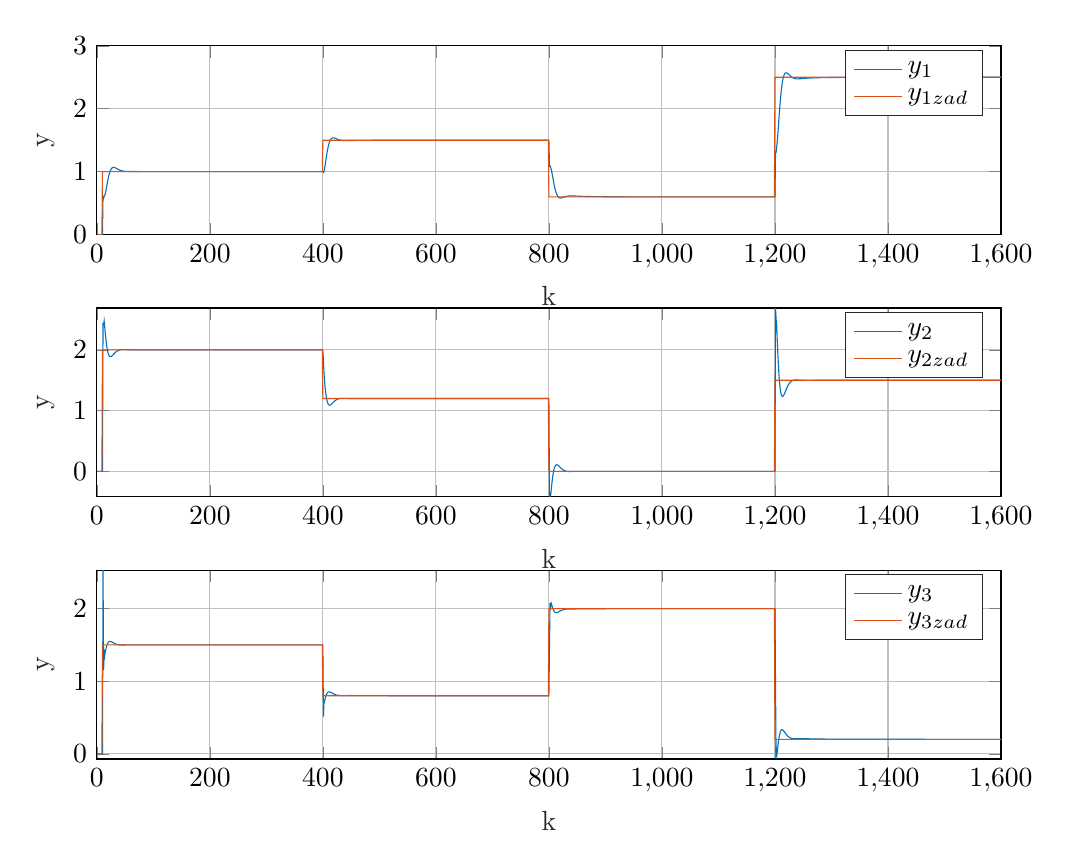
\begin{tikzpicture}

\begin{axis}[%
width=4.521in,
height=0.944in,
at={(0.758in,3.103in)},
scale only axis,
xmin=0,
xmax=1600,
xlabel style={font=\color{white!15!black}},
xlabel={k},
ymin=0,
ymax=3,
ylabel style={font=\color{white!15!black}},
ylabel={y},
axis background/.style={fill=white},
xmajorgrids,
ymajorgrids,
legend style={legend cell align=left, align=left, draw=white!15!black}
]
\addplot [color=mycolor1]
  table[row sep=crcr]{%
1	0\\
2	0\\
3	0\\
4	0\\
5	0\\
6	0\\
7	0\\
8	0\\
9	0\\
10	0\\
11	0.60656\\
12	0.57852\\
13	0.60553\\
14	0.61834\\
15	0.65034\\
16	0.69223\\
17	0.74087\\
18	0.79156\\
19	0.8411\\
20	0.8872\\
21	0.92845\\
22	0.96408\\
23	0.99385\\
24	1.0179\\
25	1.0365\\
26	1.0502\\
27	1.0597\\
28	1.0655\\
29	1.0683\\
30	1.0686\\
31	1.067\\
32	1.0641\\
33	1.0601\\
34	1.0555\\
35	1.0505\\
36	1.0455\\
37	1.0404\\
38	1.0356\\
39	1.0311\\
40	1.0269\\
41	1.0232\\
42	1.0198\\
43	1.0169\\
44	1.0143\\
45	1.0121\\
46	1.0103\\
47	1.0088\\
48	1.0075\\
49	1.0065\\
50	1.0056\\
51	1.005\\
52	1.0045\\
53	1.0041\\
54	1.0038\\
55	1.0036\\
56	1.0034\\
57	1.0033\\
58	1.0032\\
59	1.0031\\
60	1.003\\
61	1.0029\\
62	1.0029\\
63	1.0028\\
64	1.0028\\
65	1.0027\\
66	1.0026\\
67	1.0026\\
68	1.0025\\
69	1.0024\\
70	1.0023\\
71	1.0022\\
72	1.0021\\
73	1.002\\
74	1.002\\
75	1.0019\\
76	1.0018\\
77	1.0017\\
78	1.0016\\
79	1.0015\\
80	1.0014\\
81	1.0014\\
82	1.0013\\
83	1.0012\\
84	1.0011\\
85	1.0011\\
86	1.001\\
87	1.001\\
88	1.0009\\
89	1.0008\\
90	1.0008\\
91	1.0007\\
92	1.0007\\
93	1.0007\\
94	1.0006\\
95	1.0006\\
96	1.0005\\
97	1.0005\\
98	1.0005\\
99	1.0004\\
100	1.0004\\
101	1.0004\\
102	1.0004\\
103	1.0003\\
104	1.0003\\
105	1.0003\\
106	1.0003\\
107	1.0002\\
108	1.0002\\
109	1.0002\\
110	1.0002\\
111	1.0002\\
112	1.0001\\
113	1.0001\\
114	1.0001\\
115	1.0001\\
116	1.0001\\
117	1.0001\\
118	1.0001\\
119	1.0001\\
120	1\\
121	1\\
122	1\\
123	1\\
124	1\\
125	1\\
126	1\\
127	0.99999\\
128	0.99999\\
129	0.99998\\
130	0.99998\\
131	0.99997\\
132	0.99997\\
133	0.99996\\
134	0.99996\\
135	0.99996\\
136	0.99995\\
137	0.99995\\
138	0.99995\\
139	0.99994\\
140	0.99994\\
141	0.99994\\
142	0.99994\\
143	0.99993\\
144	0.99993\\
145	0.99993\\
146	0.99993\\
147	0.99993\\
148	0.99993\\
149	0.99993\\
150	0.99992\\
151	0.99992\\
152	0.99992\\
153	0.99992\\
154	0.99992\\
155	0.99992\\
156	0.99992\\
157	0.99992\\
158	0.99992\\
159	0.99992\\
160	0.99992\\
161	0.99992\\
162	0.99992\\
163	0.99992\\
164	0.99992\\
165	0.99992\\
166	0.99992\\
167	0.99992\\
168	0.99992\\
169	0.99993\\
170	0.99993\\
171	0.99993\\
172	0.99993\\
173	0.99993\\
174	0.99993\\
175	0.99993\\
176	0.99993\\
177	0.99993\\
178	0.99993\\
179	0.99993\\
180	0.99993\\
181	0.99993\\
182	0.99993\\
183	0.99994\\
184	0.99994\\
185	0.99994\\
186	0.99994\\
187	0.99994\\
188	0.99994\\
189	0.99994\\
190	0.99994\\
191	0.99994\\
192	0.99994\\
193	0.99994\\
194	0.99994\\
195	0.99995\\
196	0.99995\\
197	0.99995\\
198	0.99995\\
199	0.99995\\
200	0.99995\\
201	0.99995\\
202	0.99995\\
203	0.99995\\
204	0.99995\\
205	0.99995\\
206	0.99995\\
207	0.99996\\
208	0.99996\\
209	0.99996\\
210	0.99996\\
211	0.99996\\
212	0.99996\\
213	0.99996\\
214	0.99996\\
215	0.99996\\
216	0.99996\\
217	0.99996\\
218	0.99996\\
219	0.99996\\
220	0.99996\\
221	0.99997\\
222	0.99997\\
223	0.99997\\
224	0.99997\\
225	0.99997\\
226	0.99997\\
227	0.99997\\
228	0.99997\\
229	0.99997\\
230	0.99997\\
231	0.99997\\
232	0.99997\\
233	0.99997\\
234	0.99997\\
235	0.99997\\
236	0.99997\\
237	0.99997\\
238	0.99998\\
239	0.99998\\
240	0.99998\\
241	0.99998\\
242	0.99998\\
243	0.99998\\
244	0.99998\\
245	0.99998\\
246	0.99998\\
247	0.99998\\
248	0.99998\\
249	0.99998\\
250	0.99998\\
251	0.99998\\
252	0.99998\\
253	0.99998\\
254	0.99998\\
255	0.99998\\
256	0.99998\\
257	0.99998\\
258	0.99998\\
259	0.99998\\
260	0.99998\\
261	0.99998\\
262	0.99998\\
263	0.99999\\
264	0.99999\\
265	0.99999\\
266	0.99999\\
267	0.99999\\
268	0.99999\\
269	0.99999\\
270	0.99999\\
271	0.99999\\
272	0.99999\\
273	0.99999\\
274	0.99999\\
275	0.99999\\
276	0.99999\\
277	0.99999\\
278	0.99999\\
279	0.99999\\
280	0.99999\\
281	0.99999\\
282	0.99999\\
283	0.99999\\
284	0.99999\\
285	0.99999\\
286	0.99999\\
287	0.99999\\
288	0.99999\\
289	0.99999\\
290	0.99999\\
291	0.99999\\
292	0.99999\\
293	0.99999\\
294	0.99999\\
295	0.99999\\
296	0.99999\\
297	0.99999\\
298	0.99999\\
299	0.99999\\
300	0.99999\\
301	0.99999\\
302	0.99999\\
303	0.99999\\
304	0.99999\\
305	0.99999\\
306	0.99999\\
307	0.99999\\
308	0.99999\\
309	0.99999\\
310	0.99999\\
311	0.99999\\
312	0.99999\\
313	0.99999\\
314	1\\
315	1\\
316	1\\
317	1\\
318	1\\
319	1\\
320	1\\
321	1\\
322	1\\
323	1\\
324	1\\
325	1\\
326	1\\
327	1\\
328	1\\
329	1\\
330	1\\
331	1\\
332	1\\
333	1\\
334	1\\
335	1\\
336	1\\
337	1\\
338	1\\
339	1\\
340	1\\
341	1\\
342	1\\
343	1\\
344	1\\
345	1\\
346	1\\
347	1\\
348	1\\
349	1\\
350	1\\
351	1\\
352	1\\
353	1\\
354	1\\
355	1\\
356	1\\
357	1\\
358	1\\
359	1\\
360	1\\
361	1\\
362	1\\
363	1\\
364	1\\
365	1\\
366	1\\
367	1\\
368	1\\
369	1\\
370	1\\
371	1\\
372	1\\
373	1\\
374	1\\
375	1\\
376	1\\
377	1\\
378	1\\
379	1\\
380	1\\
381	1\\
382	1\\
383	1\\
384	1\\
385	1\\
386	1\\
387	1\\
388	1\\
389	1\\
390	1\\
391	1\\
392	1\\
393	1\\
394	1\\
395	1\\
396	1\\
397	1\\
398	1\\
399	1\\
400	1\\
401	0.98783\\
402	1.0023\\
403	1.0462\\
404	1.1024\\
405	1.1628\\
406	1.2229\\
407	1.2798\\
408	1.3315\\
409	1.3772\\
410	1.4163\\
411	1.449\\
412	1.4755\\
413	1.4963\\
414	1.512\\
415	1.5233\\
416	1.5309\\
417	1.5353\\
418	1.5373\\
419	1.5373\\
420	1.5358\\
421	1.5332\\
422	1.53\\
423	1.5263\\
424	1.5224\\
425	1.5186\\
426	1.5148\\
427	1.5113\\
428	1.5081\\
429	1.5052\\
430	1.5027\\
431	1.5006\\
432	1.4987\\
433	1.4972\\
434	1.496\\
435	1.4951\\
436	1.4944\\
437	1.4939\\
438	1.4936\\
439	1.4934\\
440	1.4933\\
441	1.4934\\
442	1.4935\\
443	1.4937\\
444	1.4939\\
445	1.4941\\
446	1.4943\\
447	1.4946\\
448	1.4948\\
449	1.4951\\
450	1.4953\\
451	1.4956\\
452	1.4958\\
453	1.496\\
454	1.4961\\
455	1.4963\\
456	1.4965\\
457	1.4966\\
458	1.4967\\
459	1.4969\\
460	1.497\\
461	1.4971\\
462	1.4972\\
463	1.4973\\
464	1.4974\\
465	1.4974\\
466	1.4975\\
467	1.4976\\
468	1.4976\\
469	1.4977\\
470	1.4978\\
471	1.4978\\
472	1.4979\\
473	1.4979\\
474	1.498\\
475	1.498\\
476	1.4981\\
477	1.4981\\
478	1.4982\\
479	1.4982\\
480	1.4983\\
481	1.4983\\
482	1.4984\\
483	1.4984\\
484	1.4985\\
485	1.4985\\
486	1.4985\\
487	1.4986\\
488	1.4986\\
489	1.4986\\
490	1.4987\\
491	1.4987\\
492	1.4987\\
493	1.4988\\
494	1.4988\\
495	1.4988\\
496	1.4989\\
497	1.4989\\
498	1.4989\\
499	1.499\\
500	1.499\\
501	1.499\\
502	1.499\\
503	1.4991\\
504	1.4991\\
505	1.4991\\
506	1.4991\\
507	1.4991\\
508	1.4992\\
509	1.4992\\
510	1.4992\\
511	1.4992\\
512	1.4992\\
513	1.4993\\
514	1.4993\\
515	1.4993\\
516	1.4993\\
517	1.4993\\
518	1.4993\\
519	1.4994\\
520	1.4994\\
521	1.4994\\
522	1.4994\\
523	1.4994\\
524	1.4994\\
525	1.4994\\
526	1.4995\\
527	1.4995\\
528	1.4995\\
529	1.4995\\
530	1.4995\\
531	1.4995\\
532	1.4995\\
533	1.4995\\
534	1.4995\\
535	1.4996\\
536	1.4996\\
537	1.4996\\
538	1.4996\\
539	1.4996\\
540	1.4996\\
541	1.4996\\
542	1.4996\\
543	1.4996\\
544	1.4996\\
545	1.4997\\
546	1.4997\\
547	1.4997\\
548	1.4997\\
549	1.4997\\
550	1.4997\\
551	1.4997\\
552	1.4997\\
553	1.4997\\
554	1.4997\\
555	1.4997\\
556	1.4997\\
557	1.4997\\
558	1.4997\\
559	1.4997\\
560	1.4998\\
561	1.4998\\
562	1.4998\\
563	1.4998\\
564	1.4998\\
565	1.4998\\
566	1.4998\\
567	1.4998\\
568	1.4998\\
569	1.4998\\
570	1.4998\\
571	1.4998\\
572	1.4998\\
573	1.4998\\
574	1.4998\\
575	1.4998\\
576	1.4998\\
577	1.4998\\
578	1.4998\\
579	1.4998\\
580	1.4998\\
581	1.4998\\
582	1.4998\\
583	1.4998\\
584	1.4999\\
585	1.4999\\
586	1.4999\\
587	1.4999\\
588	1.4999\\
589	1.4999\\
590	1.4999\\
591	1.4999\\
592	1.4999\\
593	1.4999\\
594	1.4999\\
595	1.4999\\
596	1.4999\\
597	1.4999\\
598	1.4999\\
599	1.4999\\
600	1.4999\\
601	1.4999\\
602	1.4999\\
603	1.4999\\
604	1.4999\\
605	1.4999\\
606	1.4999\\
607	1.4999\\
608	1.4999\\
609	1.4999\\
610	1.4999\\
611	1.4999\\
612	1.4999\\
613	1.4999\\
614	1.4999\\
615	1.4999\\
616	1.4999\\
617	1.4999\\
618	1.4999\\
619	1.4999\\
620	1.4999\\
621	1.4999\\
622	1.4999\\
623	1.4999\\
624	1.4999\\
625	1.4999\\
626	1.4999\\
627	1.4999\\
628	1.4999\\
629	1.4999\\
630	1.4999\\
631	1.4999\\
632	1.4999\\
633	1.4999\\
634	1.5\\
635	1.5\\
636	1.5\\
637	1.5\\
638	1.5\\
639	1.5\\
640	1.5\\
641	1.5\\
642	1.5\\
643	1.5\\
644	1.5\\
645	1.5\\
646	1.5\\
647	1.5\\
648	1.5\\
649	1.5\\
650	1.5\\
651	1.5\\
652	1.5\\
653	1.5\\
654	1.5\\
655	1.5\\
656	1.5\\
657	1.5\\
658	1.5\\
659	1.5\\
660	1.5\\
661	1.5\\
662	1.5\\
663	1.5\\
664	1.5\\
665	1.5\\
666	1.5\\
667	1.5\\
668	1.5\\
669	1.5\\
670	1.5\\
671	1.5\\
672	1.5\\
673	1.5\\
674	1.5\\
675	1.5\\
676	1.5\\
677	1.5\\
678	1.5\\
679	1.5\\
680	1.5\\
681	1.5\\
682	1.5\\
683	1.5\\
684	1.5\\
685	1.5\\
686	1.5\\
687	1.5\\
688	1.5\\
689	1.5\\
690	1.5\\
691	1.5\\
692	1.5\\
693	1.5\\
694	1.5\\
695	1.5\\
696	1.5\\
697	1.5\\
698	1.5\\
699	1.5\\
700	1.5\\
701	1.5\\
702	1.5\\
703	1.5\\
704	1.5\\
705	1.5\\
706	1.5\\
707	1.5\\
708	1.5\\
709	1.5\\
710	1.5\\
711	1.5\\
712	1.5\\
713	1.5\\
714	1.5\\
715	1.5\\
716	1.5\\
717	1.5\\
718	1.5\\
719	1.5\\
720	1.5\\
721	1.5\\
722	1.5\\
723	1.5\\
724	1.5\\
725	1.5\\
726	1.5\\
727	1.5\\
728	1.5\\
729	1.5\\
730	1.5\\
731	1.5\\
732	1.5\\
733	1.5\\
734	1.5\\
735	1.5\\
736	1.5\\
737	1.5\\
738	1.5\\
739	1.5\\
740	1.5\\
741	1.5\\
742	1.5\\
743	1.5\\
744	1.5\\
745	1.5\\
746	1.5\\
747	1.5\\
748	1.5\\
749	1.5\\
750	1.5\\
751	1.5\\
752	1.5\\
753	1.5\\
754	1.5\\
755	1.5\\
756	1.5\\
757	1.5\\
758	1.5\\
759	1.5\\
760	1.5\\
761	1.5\\
762	1.5\\
763	1.5\\
764	1.5\\
765	1.5\\
766	1.5\\
767	1.5\\
768	1.5\\
769	1.5\\
770	1.5\\
771	1.5\\
772	1.5\\
773	1.5\\
774	1.5\\
775	1.5\\
776	1.5\\
777	1.5\\
778	1.5\\
779	1.5\\
780	1.5\\
781	1.5\\
782	1.5\\
783	1.5\\
784	1.5\\
785	1.5\\
786	1.5\\
787	1.5\\
788	1.5\\
789	1.5\\
790	1.5\\
791	1.5\\
792	1.5\\
793	1.5\\
794	1.5\\
795	1.5\\
796	1.5\\
797	1.5\\
798	1.5\\
799	1.5\\
800	1.5\\
801	1.0876\\
802	1.0927\\
803	1.0649\\
804	1.0401\\
805	1.0015\\
806	0.95537\\
807	0.90512\\
808	0.85448\\
809	0.80601\\
810	0.76149\\
811	0.72194\\
812	0.68788\\
813	0.65938\\
814	0.63624\\
815	0.61807\\
816	0.60434\\
817	0.59449\\
818	0.58793\\
819	0.58409\\
820	0.58242\\
821	0.58246\\
822	0.58375\\
823	0.58595\\
824	0.58872\\
825	0.59182\\
826	0.59505\\
827	0.59825\\
828	0.60129\\
829	0.6041\\
830	0.60662\\
831	0.60882\\
832	0.61069\\
833	0.61224\\
834	0.61347\\
835	0.61441\\
836	0.61509\\
837	0.61553\\
838	0.61576\\
839	0.61582\\
840	0.61573\\
841	0.61553\\
842	0.61522\\
843	0.61485\\
844	0.61442\\
845	0.61395\\
846	0.61346\\
847	0.61296\\
848	0.61245\\
849	0.61195\\
850	0.61147\\
851	0.611\\
852	0.61054\\
853	0.61011\\
854	0.6097\\
855	0.60931\\
856	0.60894\\
857	0.60859\\
858	0.60826\\
859	0.60795\\
860	0.60766\\
861	0.60739\\
862	0.60712\\
863	0.60688\\
864	0.60664\\
865	0.60642\\
866	0.60621\\
867	0.60601\\
868	0.60582\\
869	0.60563\\
870	0.60545\\
871	0.60528\\
872	0.60512\\
873	0.60496\\
874	0.60481\\
875	0.60466\\
876	0.60452\\
877	0.60438\\
878	0.60425\\
879	0.60412\\
880	0.60399\\
881	0.60387\\
882	0.60376\\
883	0.60364\\
884	0.60353\\
885	0.60343\\
886	0.60333\\
887	0.60323\\
888	0.60313\\
889	0.60304\\
890	0.60295\\
891	0.60286\\
892	0.60278\\
893	0.6027\\
894	0.60262\\
895	0.60254\\
896	0.60247\\
897	0.6024\\
898	0.60233\\
899	0.60227\\
900	0.6022\\
901	0.60214\\
902	0.60208\\
903	0.60202\\
904	0.60196\\
905	0.60191\\
906	0.60186\\
907	0.60181\\
908	0.60176\\
909	0.60171\\
910	0.60166\\
911	0.60162\\
912	0.60157\\
913	0.60153\\
914	0.60149\\
915	0.60145\\
916	0.60141\\
917	0.60137\\
918	0.60134\\
919	0.6013\\
920	0.60127\\
921	0.60123\\
922	0.6012\\
923	0.60117\\
924	0.60114\\
925	0.60111\\
926	0.60108\\
927	0.60106\\
928	0.60103\\
929	0.601\\
930	0.60098\\
931	0.60095\\
932	0.60093\\
933	0.60091\\
934	0.60088\\
935	0.60086\\
936	0.60084\\
937	0.60082\\
938	0.6008\\
939	0.60078\\
940	0.60076\\
941	0.60074\\
942	0.60072\\
943	0.6007\\
944	0.60069\\
945	0.60067\\
946	0.60065\\
947	0.60064\\
948	0.60062\\
949	0.60061\\
950	0.60059\\
951	0.60058\\
952	0.60057\\
953	0.60055\\
954	0.60054\\
955	0.60053\\
956	0.60051\\
957	0.6005\\
958	0.60049\\
959	0.60048\\
960	0.60047\\
961	0.60046\\
962	0.60045\\
963	0.60044\\
964	0.60043\\
965	0.60042\\
966	0.60041\\
967	0.6004\\
968	0.60039\\
969	0.60038\\
970	0.60037\\
971	0.60036\\
972	0.60035\\
973	0.60035\\
974	0.60034\\
975	0.60033\\
976	0.60032\\
977	0.60031\\
978	0.60031\\
979	0.6003\\
980	0.60029\\
981	0.60029\\
982	0.60028\\
983	0.60027\\
984	0.60027\\
985	0.60026\\
986	0.60026\\
987	0.60025\\
988	0.60025\\
989	0.60024\\
990	0.60023\\
991	0.60023\\
992	0.60022\\
993	0.60022\\
994	0.60021\\
995	0.60021\\
996	0.6002\\
997	0.6002\\
998	0.6002\\
999	0.60019\\
1000	0.60019\\
1001	0.60018\\
1002	0.60018\\
1003	0.60017\\
1004	0.60017\\
1005	0.60017\\
1006	0.60016\\
1007	0.60016\\
1008	0.60016\\
1009	0.60015\\
1010	0.60015\\
1011	0.60015\\
1012	0.60014\\
1013	0.60014\\
1014	0.60014\\
1015	0.60013\\
1016	0.60013\\
1017	0.60013\\
1018	0.60013\\
1019	0.60012\\
1020	0.60012\\
1021	0.60012\\
1022	0.60011\\
1023	0.60011\\
1024	0.60011\\
1025	0.60011\\
1026	0.60011\\
1027	0.6001\\
1028	0.6001\\
1029	0.6001\\
1030	0.6001\\
1031	0.60009\\
1032	0.60009\\
1033	0.60009\\
1034	0.60009\\
1035	0.60009\\
1036	0.60008\\
1037	0.60008\\
1038	0.60008\\
1039	0.60008\\
1040	0.60008\\
1041	0.60008\\
1042	0.60007\\
1043	0.60007\\
1044	0.60007\\
1045	0.60007\\
1046	0.60007\\
1047	0.60007\\
1048	0.60006\\
1049	0.60006\\
1050	0.60006\\
1051	0.60006\\
1052	0.60006\\
1053	0.60006\\
1054	0.60006\\
1055	0.60006\\
1056	0.60005\\
1057	0.60005\\
1058	0.60005\\
1059	0.60005\\
1060	0.60005\\
1061	0.60005\\
1062	0.60005\\
1063	0.60005\\
1064	0.60005\\
1065	0.60004\\
1066	0.60004\\
1067	0.60004\\
1068	0.60004\\
1069	0.60004\\
1070	0.60004\\
1071	0.60004\\
1072	0.60004\\
1073	0.60004\\
1074	0.60004\\
1075	0.60004\\
1076	0.60004\\
1077	0.60003\\
1078	0.60003\\
1079	0.60003\\
1080	0.60003\\
1081	0.60003\\
1082	0.60003\\
1083	0.60003\\
1084	0.60003\\
1085	0.60003\\
1086	0.60003\\
1087	0.60003\\
1088	0.60003\\
1089	0.60003\\
1090	0.60003\\
1091	0.60003\\
1092	0.60002\\
1093	0.60002\\
1094	0.60002\\
1095	0.60002\\
1096	0.60002\\
1097	0.60002\\
1098	0.60002\\
1099	0.60002\\
1100	0.60002\\
1101	0.60002\\
1102	0.60002\\
1103	0.60002\\
1104	0.60002\\
1105	0.60002\\
1106	0.60002\\
1107	0.60002\\
1108	0.60002\\
1109	0.60002\\
1110	0.60002\\
1111	0.60002\\
1112	0.60002\\
1113	0.60002\\
1114	0.60002\\
1115	0.60001\\
1116	0.60001\\
1117	0.60001\\
1118	0.60001\\
1119	0.60001\\
1120	0.60001\\
1121	0.60001\\
1122	0.60001\\
1123	0.60001\\
1124	0.60001\\
1125	0.60001\\
1126	0.60001\\
1127	0.60001\\
1128	0.60001\\
1129	0.60001\\
1130	0.60001\\
1131	0.60001\\
1132	0.60001\\
1133	0.60001\\
1134	0.60001\\
1135	0.60001\\
1136	0.60001\\
1137	0.60001\\
1138	0.60001\\
1139	0.60001\\
1140	0.60001\\
1141	0.60001\\
1142	0.60001\\
1143	0.60001\\
1144	0.60001\\
1145	0.60001\\
1146	0.60001\\
1147	0.60001\\
1148	0.60001\\
1149	0.60001\\
1150	0.60001\\
1151	0.60001\\
1152	0.60001\\
1153	0.60001\\
1154	0.60001\\
1155	0.60001\\
1156	0.60001\\
1157	0.60001\\
1158	0.60001\\
1159	0.60001\\
1160	0.60001\\
1161	0.60001\\
1162	0.60001\\
1163	0.60001\\
1164	0.60001\\
1165	0.6\\
1166	0.6\\
1167	0.6\\
1168	0.6\\
1169	0.6\\
1170	0.6\\
1171	0.6\\
1172	0.6\\
1173	0.6\\
1174	0.6\\
1175	0.6\\
1176	0.6\\
1177	0.6\\
1178	0.6\\
1179	0.6\\
1180	0.6\\
1181	0.6\\
1182	0.6\\
1183	0.6\\
1184	0.6\\
1185	0.6\\
1186	0.6\\
1187	0.6\\
1188	0.6\\
1189	0.6\\
1190	0.6\\
1191	0.6\\
1192	0.6\\
1193	0.6\\
1194	0.6\\
1195	0.6\\
1196	0.6\\
1197	0.6\\
1198	0.6\\
1199	0.6\\
1200	0.6\\
1201	1.311\\
1202	1.3086\\
1203	1.3896\\
1204	1.4732\\
1205	1.584\\
1206	1.7073\\
1207	1.8354\\
1208	1.9603\\
1209	2.0769\\
1210	2.182\\
1211	2.2736\\
1212	2.3511\\
1213	2.4149\\
1214	2.4657\\
1215	2.5046\\
1216	2.5331\\
1217	2.5527\\
1218	2.5647\\
1219	2.5707\\
1220	2.5718\\
1221	2.5692\\
1222	2.564\\
1223	2.5569\\
1224	2.5487\\
1225	2.54\\
1226	2.5312\\
1227	2.5226\\
1228	2.5145\\
1229	2.5071\\
1230	2.5005\\
1231	2.4948\\
1232	2.4898\\
1233	2.4857\\
1234	2.4823\\
1235	2.4797\\
1236	2.4777\\
1237	2.4763\\
1238	2.4754\\
1239	2.4749\\
1240	2.4747\\
1241	2.4749\\
1242	2.4752\\
1243	2.4758\\
1244	2.4764\\
1245	2.4772\\
1246	2.478\\
1247	2.4789\\
1248	2.4797\\
1249	2.4806\\
1250	2.4814\\
1251	2.4822\\
1252	2.483\\
1253	2.4837\\
1254	2.4844\\
1255	2.4851\\
1256	2.4857\\
1257	2.4863\\
1258	2.4868\\
1259	2.4873\\
1260	2.4878\\
1261	2.4882\\
1262	2.4886\\
1263	2.489\\
1264	2.4893\\
1265	2.4897\\
1266	2.49\\
1267	2.4903\\
1268	2.4906\\
1269	2.4909\\
1270	2.4912\\
1271	2.4914\\
1272	2.4917\\
1273	2.4919\\
1274	2.4921\\
1275	2.4924\\
1276	2.4926\\
1277	2.4928\\
1278	2.493\\
1279	2.4932\\
1280	2.4934\\
1281	2.4936\\
1282	2.4938\\
1283	2.4939\\
1284	2.4941\\
1285	2.4943\\
1286	2.4944\\
1287	2.4946\\
1288	2.4947\\
1289	2.4949\\
1290	2.495\\
1291	2.4952\\
1292	2.4953\\
1293	2.4954\\
1294	2.4956\\
1295	2.4957\\
1296	2.4958\\
1297	2.4959\\
1298	2.496\\
1299	2.4961\\
1300	2.4962\\
1301	2.4963\\
1302	2.4964\\
1303	2.4965\\
1304	2.4966\\
1305	2.4967\\
1306	2.4968\\
1307	2.4969\\
1308	2.497\\
1309	2.497\\
1310	2.4971\\
1311	2.4972\\
1312	2.4973\\
1313	2.4973\\
1314	2.4974\\
1315	2.4975\\
1316	2.4975\\
1317	2.4976\\
1318	2.4976\\
1319	2.4977\\
1320	2.4978\\
1321	2.4978\\
1322	2.4979\\
1323	2.4979\\
1324	2.498\\
1325	2.498\\
1326	2.4981\\
1327	2.4981\\
1328	2.4982\\
1329	2.4982\\
1330	2.4983\\
1331	2.4983\\
1332	2.4983\\
1333	2.4984\\
1334	2.4984\\
1335	2.4985\\
1336	2.4985\\
1337	2.4985\\
1338	2.4986\\
1339	2.4986\\
1340	2.4986\\
1341	2.4987\\
1342	2.4987\\
1343	2.4987\\
1344	2.4988\\
1345	2.4988\\
1346	2.4988\\
1347	2.4988\\
1348	2.4989\\
1349	2.4989\\
1350	2.4989\\
1351	2.4989\\
1352	2.499\\
1353	2.499\\
1354	2.499\\
1355	2.499\\
1356	2.4991\\
1357	2.4991\\
1358	2.4991\\
1359	2.4991\\
1360	2.4991\\
1361	2.4992\\
1362	2.4992\\
1363	2.4992\\
1364	2.4992\\
1365	2.4992\\
1366	2.4993\\
1367	2.4993\\
1368	2.4993\\
1369	2.4993\\
1370	2.4993\\
1371	2.4993\\
1372	2.4993\\
1373	2.4994\\
1374	2.4994\\
1375	2.4994\\
1376	2.4994\\
1377	2.4994\\
1378	2.4994\\
1379	2.4994\\
1380	2.4995\\
1381	2.4995\\
1382	2.4995\\
1383	2.4995\\
1384	2.4995\\
1385	2.4995\\
1386	2.4995\\
1387	2.4995\\
1388	2.4995\\
1389	2.4996\\
1390	2.4996\\
1391	2.4996\\
1392	2.4996\\
1393	2.4996\\
1394	2.4996\\
1395	2.4996\\
1396	2.4996\\
1397	2.4996\\
1398	2.4996\\
1399	2.4996\\
1400	2.4996\\
1401	2.4997\\
1402	2.4997\\
1403	2.4997\\
1404	2.4997\\
1405	2.4997\\
1406	2.4997\\
1407	2.4997\\
1408	2.4997\\
1409	2.4997\\
1410	2.4997\\
1411	2.4997\\
1412	2.4997\\
1413	2.4997\\
1414	2.4997\\
1415	2.4997\\
1416	2.4998\\
1417	2.4998\\
1418	2.4998\\
1419	2.4998\\
1420	2.4998\\
1421	2.4998\\
1422	2.4998\\
1423	2.4998\\
1424	2.4998\\
1425	2.4998\\
1426	2.4998\\
1427	2.4998\\
1428	2.4998\\
1429	2.4998\\
1430	2.4998\\
1431	2.4998\\
1432	2.4998\\
1433	2.4998\\
1434	2.4998\\
1435	2.4998\\
1436	2.4998\\
1437	2.4998\\
1438	2.4998\\
1439	2.4999\\
1440	2.4999\\
1441	2.4999\\
1442	2.4999\\
1443	2.4999\\
1444	2.4999\\
1445	2.4999\\
1446	2.4999\\
1447	2.4999\\
1448	2.4999\\
1449	2.4999\\
1450	2.4999\\
1451	2.4999\\
1452	2.4999\\
1453	2.4999\\
1454	2.4999\\
1455	2.4999\\
1456	2.4999\\
1457	2.4999\\
1458	2.4999\\
1459	2.4999\\
1460	2.4999\\
1461	2.4999\\
1462	2.4999\\
1463	2.4999\\
1464	2.4999\\
1465	2.4999\\
1466	2.4999\\
1467	2.4999\\
1468	2.4999\\
1469	2.4999\\
1470	2.4999\\
1471	2.4999\\
1472	2.4999\\
1473	2.4999\\
1474	2.4999\\
1475	2.4999\\
1476	2.4999\\
1477	2.4999\\
1478	2.4999\\
1479	2.4999\\
1480	2.4999\\
1481	2.4999\\
1482	2.4999\\
1483	2.4999\\
1484	2.4999\\
1485	2.4999\\
1486	2.4999\\
1487	2.4999\\
1488	2.4999\\
1489	2.5\\
1490	2.5\\
1491	2.5\\
1492	2.5\\
1493	2.5\\
1494	2.5\\
1495	2.5\\
1496	2.5\\
1497	2.5\\
1498	2.5\\
1499	2.5\\
1500	2.5\\
1501	2.5\\
1502	2.5\\
1503	2.5\\
1504	2.5\\
1505	2.5\\
1506	2.5\\
1507	2.5\\
1508	2.5\\
1509	2.5\\
1510	2.5\\
1511	2.5\\
1512	2.5\\
1513	2.5\\
1514	2.5\\
1515	2.5\\
1516	2.5\\
1517	2.5\\
1518	2.5\\
1519	2.5\\
1520	2.5\\
1521	2.5\\
1522	2.5\\
1523	2.5\\
1524	2.5\\
1525	2.5\\
1526	2.5\\
1527	2.5\\
1528	2.5\\
1529	2.5\\
1530	2.5\\
1531	2.5\\
1532	2.5\\
1533	2.5\\
1534	2.5\\
1535	2.5\\
1536	2.5\\
1537	2.5\\
1538	2.5\\
1539	2.5\\
1540	2.5\\
1541	2.5\\
1542	2.5\\
1543	2.5\\
1544	2.5\\
1545	2.5\\
1546	2.5\\
1547	2.5\\
1548	2.5\\
1549	2.5\\
1550	2.5\\
1551	2.5\\
1552	2.5\\
1553	2.5\\
1554	2.5\\
1555	2.5\\
1556	2.5\\
1557	2.5\\
1558	2.5\\
1559	2.5\\
1560	2.5\\
1561	2.5\\
1562	2.5\\
1563	2.5\\
1564	2.5\\
1565	2.5\\
1566	2.5\\
1567	2.5\\
1568	2.5\\
1569	2.5\\
1570	2.5\\
1571	2.5\\
1572	2.5\\
1573	2.5\\
1574	2.5\\
1575	2.5\\
1576	2.5\\
1577	2.5\\
1578	2.5\\
1579	2.5\\
1580	2.5\\
1581	2.5\\
1582	2.5\\
1583	2.5\\
1584	2.5\\
1585	2.5\\
1586	2.5\\
1587	2.5\\
1588	2.5\\
1589	2.5\\
1590	2.5\\
1591	2.5\\
1592	2.5\\
1593	2.5\\
1594	2.5\\
1595	2.5\\
1596	2.5\\
1597	2.5\\
1598	2.5\\
1599	2.5\\
1600	2.5\\
};
\addlegendentry{$\text{y}_\text{1}$}

\addplot [color=mycolor2]
  table[row sep=crcr]{%
1	0\\
2	0\\
3	0\\
4	0\\
5	0\\
6	0\\
7	0\\
8	0\\
9	0\\
10	1\\
11	1\\
12	1\\
13	1\\
14	1\\
15	1\\
16	1\\
17	1\\
18	1\\
19	1\\
20	1\\
21	1\\
22	1\\
23	1\\
24	1\\
25	1\\
26	1\\
27	1\\
28	1\\
29	1\\
30	1\\
31	1\\
32	1\\
33	1\\
34	1\\
35	1\\
36	1\\
37	1\\
38	1\\
39	1\\
40	1\\
41	1\\
42	1\\
43	1\\
44	1\\
45	1\\
46	1\\
47	1\\
48	1\\
49	1\\
50	1\\
51	1\\
52	1\\
53	1\\
54	1\\
55	1\\
56	1\\
57	1\\
58	1\\
59	1\\
60	1\\
61	1\\
62	1\\
63	1\\
64	1\\
65	1\\
66	1\\
67	1\\
68	1\\
69	1\\
70	1\\
71	1\\
72	1\\
73	1\\
74	1\\
75	1\\
76	1\\
77	1\\
78	1\\
79	1\\
80	1\\
81	1\\
82	1\\
83	1\\
84	1\\
85	1\\
86	1\\
87	1\\
88	1\\
89	1\\
90	1\\
91	1\\
92	1\\
93	1\\
94	1\\
95	1\\
96	1\\
97	1\\
98	1\\
99	1\\
100	1\\
101	1\\
102	1\\
103	1\\
104	1\\
105	1\\
106	1\\
107	1\\
108	1\\
109	1\\
110	1\\
111	1\\
112	1\\
113	1\\
114	1\\
115	1\\
116	1\\
117	1\\
118	1\\
119	1\\
120	1\\
121	1\\
122	1\\
123	1\\
124	1\\
125	1\\
126	1\\
127	1\\
128	1\\
129	1\\
130	1\\
131	1\\
132	1\\
133	1\\
134	1\\
135	1\\
136	1\\
137	1\\
138	1\\
139	1\\
140	1\\
141	1\\
142	1\\
143	1\\
144	1\\
145	1\\
146	1\\
147	1\\
148	1\\
149	1\\
150	1\\
151	1\\
152	1\\
153	1\\
154	1\\
155	1\\
156	1\\
157	1\\
158	1\\
159	1\\
160	1\\
161	1\\
162	1\\
163	1\\
164	1\\
165	1\\
166	1\\
167	1\\
168	1\\
169	1\\
170	1\\
171	1\\
172	1\\
173	1\\
174	1\\
175	1\\
176	1\\
177	1\\
178	1\\
179	1\\
180	1\\
181	1\\
182	1\\
183	1\\
184	1\\
185	1\\
186	1\\
187	1\\
188	1\\
189	1\\
190	1\\
191	1\\
192	1\\
193	1\\
194	1\\
195	1\\
196	1\\
197	1\\
198	1\\
199	1\\
200	1\\
201	1\\
202	1\\
203	1\\
204	1\\
205	1\\
206	1\\
207	1\\
208	1\\
209	1\\
210	1\\
211	1\\
212	1\\
213	1\\
214	1\\
215	1\\
216	1\\
217	1\\
218	1\\
219	1\\
220	1\\
221	1\\
222	1\\
223	1\\
224	1\\
225	1\\
226	1\\
227	1\\
228	1\\
229	1\\
230	1\\
231	1\\
232	1\\
233	1\\
234	1\\
235	1\\
236	1\\
237	1\\
238	1\\
239	1\\
240	1\\
241	1\\
242	1\\
243	1\\
244	1\\
245	1\\
246	1\\
247	1\\
248	1\\
249	1\\
250	1\\
251	1\\
252	1\\
253	1\\
254	1\\
255	1\\
256	1\\
257	1\\
258	1\\
259	1\\
260	1\\
261	1\\
262	1\\
263	1\\
264	1\\
265	1\\
266	1\\
267	1\\
268	1\\
269	1\\
270	1\\
271	1\\
272	1\\
273	1\\
274	1\\
275	1\\
276	1\\
277	1\\
278	1\\
279	1\\
280	1\\
281	1\\
282	1\\
283	1\\
284	1\\
285	1\\
286	1\\
287	1\\
288	1\\
289	1\\
290	1\\
291	1\\
292	1\\
293	1\\
294	1\\
295	1\\
296	1\\
297	1\\
298	1\\
299	1\\
300	1\\
301	1\\
302	1\\
303	1\\
304	1\\
305	1\\
306	1\\
307	1\\
308	1\\
309	1\\
310	1\\
311	1\\
312	1\\
313	1\\
314	1\\
315	1\\
316	1\\
317	1\\
318	1\\
319	1\\
320	1\\
321	1\\
322	1\\
323	1\\
324	1\\
325	1\\
326	1\\
327	1\\
328	1\\
329	1\\
330	1\\
331	1\\
332	1\\
333	1\\
334	1\\
335	1\\
336	1\\
337	1\\
338	1\\
339	1\\
340	1\\
341	1\\
342	1\\
343	1\\
344	1\\
345	1\\
346	1\\
347	1\\
348	1\\
349	1\\
350	1\\
351	1\\
352	1\\
353	1\\
354	1\\
355	1\\
356	1\\
357	1\\
358	1\\
359	1\\
360	1\\
361	1\\
362	1\\
363	1\\
364	1\\
365	1\\
366	1\\
367	1\\
368	1\\
369	1\\
370	1\\
371	1\\
372	1\\
373	1\\
374	1\\
375	1\\
376	1\\
377	1\\
378	1\\
379	1\\
380	1\\
381	1\\
382	1\\
383	1\\
384	1\\
385	1\\
386	1\\
387	1\\
388	1\\
389	1\\
390	1\\
391	1\\
392	1\\
393	1\\
394	1\\
395	1\\
396	1\\
397	1\\
398	1\\
399	1\\
400	1.5\\
401	1.5\\
402	1.5\\
403	1.5\\
404	1.5\\
405	1.5\\
406	1.5\\
407	1.5\\
408	1.5\\
409	1.5\\
410	1.5\\
411	1.5\\
412	1.5\\
413	1.5\\
414	1.5\\
415	1.5\\
416	1.5\\
417	1.5\\
418	1.5\\
419	1.5\\
420	1.5\\
421	1.5\\
422	1.5\\
423	1.5\\
424	1.5\\
425	1.5\\
426	1.5\\
427	1.5\\
428	1.5\\
429	1.5\\
430	1.5\\
431	1.5\\
432	1.5\\
433	1.5\\
434	1.5\\
435	1.5\\
436	1.5\\
437	1.5\\
438	1.5\\
439	1.5\\
440	1.5\\
441	1.5\\
442	1.5\\
443	1.5\\
444	1.5\\
445	1.5\\
446	1.5\\
447	1.5\\
448	1.5\\
449	1.5\\
450	1.5\\
451	1.5\\
452	1.5\\
453	1.5\\
454	1.5\\
455	1.5\\
456	1.5\\
457	1.5\\
458	1.5\\
459	1.5\\
460	1.5\\
461	1.5\\
462	1.5\\
463	1.5\\
464	1.5\\
465	1.5\\
466	1.5\\
467	1.5\\
468	1.5\\
469	1.5\\
470	1.5\\
471	1.5\\
472	1.5\\
473	1.5\\
474	1.5\\
475	1.5\\
476	1.5\\
477	1.5\\
478	1.5\\
479	1.5\\
480	1.5\\
481	1.5\\
482	1.5\\
483	1.5\\
484	1.5\\
485	1.5\\
486	1.5\\
487	1.5\\
488	1.5\\
489	1.5\\
490	1.5\\
491	1.5\\
492	1.5\\
493	1.5\\
494	1.5\\
495	1.5\\
496	1.5\\
497	1.5\\
498	1.5\\
499	1.5\\
500	1.5\\
501	1.5\\
502	1.5\\
503	1.5\\
504	1.5\\
505	1.5\\
506	1.5\\
507	1.5\\
508	1.5\\
509	1.5\\
510	1.5\\
511	1.5\\
512	1.5\\
513	1.5\\
514	1.5\\
515	1.5\\
516	1.5\\
517	1.5\\
518	1.5\\
519	1.5\\
520	1.5\\
521	1.5\\
522	1.5\\
523	1.5\\
524	1.5\\
525	1.5\\
526	1.5\\
527	1.5\\
528	1.5\\
529	1.5\\
530	1.5\\
531	1.5\\
532	1.5\\
533	1.5\\
534	1.5\\
535	1.5\\
536	1.5\\
537	1.5\\
538	1.5\\
539	1.5\\
540	1.5\\
541	1.5\\
542	1.5\\
543	1.5\\
544	1.5\\
545	1.5\\
546	1.5\\
547	1.5\\
548	1.5\\
549	1.5\\
550	1.5\\
551	1.5\\
552	1.5\\
553	1.5\\
554	1.5\\
555	1.5\\
556	1.5\\
557	1.5\\
558	1.5\\
559	1.5\\
560	1.5\\
561	1.5\\
562	1.5\\
563	1.5\\
564	1.5\\
565	1.5\\
566	1.5\\
567	1.5\\
568	1.5\\
569	1.5\\
570	1.5\\
571	1.5\\
572	1.5\\
573	1.5\\
574	1.5\\
575	1.5\\
576	1.5\\
577	1.5\\
578	1.5\\
579	1.5\\
580	1.5\\
581	1.5\\
582	1.5\\
583	1.5\\
584	1.5\\
585	1.5\\
586	1.5\\
587	1.5\\
588	1.5\\
589	1.5\\
590	1.5\\
591	1.5\\
592	1.5\\
593	1.5\\
594	1.5\\
595	1.5\\
596	1.5\\
597	1.5\\
598	1.5\\
599	1.5\\
600	1.5\\
601	1.5\\
602	1.5\\
603	1.5\\
604	1.5\\
605	1.5\\
606	1.5\\
607	1.5\\
608	1.5\\
609	1.5\\
610	1.5\\
611	1.5\\
612	1.5\\
613	1.5\\
614	1.5\\
615	1.5\\
616	1.5\\
617	1.5\\
618	1.5\\
619	1.5\\
620	1.5\\
621	1.5\\
622	1.5\\
623	1.5\\
624	1.5\\
625	1.5\\
626	1.5\\
627	1.5\\
628	1.5\\
629	1.5\\
630	1.5\\
631	1.5\\
632	1.5\\
633	1.5\\
634	1.5\\
635	1.5\\
636	1.5\\
637	1.5\\
638	1.5\\
639	1.5\\
640	1.5\\
641	1.5\\
642	1.5\\
643	1.5\\
644	1.5\\
645	1.5\\
646	1.5\\
647	1.5\\
648	1.5\\
649	1.5\\
650	1.5\\
651	1.5\\
652	1.5\\
653	1.5\\
654	1.5\\
655	1.5\\
656	1.5\\
657	1.5\\
658	1.5\\
659	1.5\\
660	1.5\\
661	1.5\\
662	1.5\\
663	1.5\\
664	1.5\\
665	1.5\\
666	1.5\\
667	1.5\\
668	1.5\\
669	1.5\\
670	1.5\\
671	1.5\\
672	1.5\\
673	1.5\\
674	1.5\\
675	1.5\\
676	1.5\\
677	1.5\\
678	1.5\\
679	1.5\\
680	1.5\\
681	1.5\\
682	1.5\\
683	1.5\\
684	1.5\\
685	1.5\\
686	1.5\\
687	1.5\\
688	1.5\\
689	1.5\\
690	1.5\\
691	1.5\\
692	1.5\\
693	1.5\\
694	1.5\\
695	1.5\\
696	1.5\\
697	1.5\\
698	1.5\\
699	1.5\\
700	1.5\\
701	1.5\\
702	1.5\\
703	1.5\\
704	1.5\\
705	1.5\\
706	1.5\\
707	1.5\\
708	1.5\\
709	1.5\\
710	1.5\\
711	1.5\\
712	1.5\\
713	1.5\\
714	1.5\\
715	1.5\\
716	1.5\\
717	1.5\\
718	1.5\\
719	1.5\\
720	1.5\\
721	1.5\\
722	1.5\\
723	1.5\\
724	1.5\\
725	1.5\\
726	1.5\\
727	1.5\\
728	1.5\\
729	1.5\\
730	1.5\\
731	1.5\\
732	1.5\\
733	1.5\\
734	1.5\\
735	1.5\\
736	1.5\\
737	1.5\\
738	1.5\\
739	1.5\\
740	1.5\\
741	1.5\\
742	1.5\\
743	1.5\\
744	1.5\\
745	1.5\\
746	1.5\\
747	1.5\\
748	1.5\\
749	1.5\\
750	1.5\\
751	1.5\\
752	1.5\\
753	1.5\\
754	1.5\\
755	1.5\\
756	1.5\\
757	1.5\\
758	1.5\\
759	1.5\\
760	1.5\\
761	1.5\\
762	1.5\\
763	1.5\\
764	1.5\\
765	1.5\\
766	1.5\\
767	1.5\\
768	1.5\\
769	1.5\\
770	1.5\\
771	1.5\\
772	1.5\\
773	1.5\\
774	1.5\\
775	1.5\\
776	1.5\\
777	1.5\\
778	1.5\\
779	1.5\\
780	1.5\\
781	1.5\\
782	1.5\\
783	1.5\\
784	1.5\\
785	1.5\\
786	1.5\\
787	1.5\\
788	1.5\\
789	1.5\\
790	1.5\\
791	1.5\\
792	1.5\\
793	1.5\\
794	1.5\\
795	1.5\\
796	1.5\\
797	1.5\\
798	1.5\\
799	1.5\\
800	0.6\\
801	0.6\\
802	0.6\\
803	0.6\\
804	0.6\\
805	0.6\\
806	0.6\\
807	0.6\\
808	0.6\\
809	0.6\\
810	0.6\\
811	0.6\\
812	0.6\\
813	0.6\\
814	0.6\\
815	0.6\\
816	0.6\\
817	0.6\\
818	0.6\\
819	0.6\\
820	0.6\\
821	0.6\\
822	0.6\\
823	0.6\\
824	0.6\\
825	0.6\\
826	0.6\\
827	0.6\\
828	0.6\\
829	0.6\\
830	0.6\\
831	0.6\\
832	0.6\\
833	0.6\\
834	0.6\\
835	0.6\\
836	0.6\\
837	0.6\\
838	0.6\\
839	0.6\\
840	0.6\\
841	0.6\\
842	0.6\\
843	0.6\\
844	0.6\\
845	0.6\\
846	0.6\\
847	0.6\\
848	0.6\\
849	0.6\\
850	0.6\\
851	0.6\\
852	0.6\\
853	0.6\\
854	0.6\\
855	0.6\\
856	0.6\\
857	0.6\\
858	0.6\\
859	0.6\\
860	0.6\\
861	0.6\\
862	0.6\\
863	0.6\\
864	0.6\\
865	0.6\\
866	0.6\\
867	0.6\\
868	0.6\\
869	0.6\\
870	0.6\\
871	0.6\\
872	0.6\\
873	0.6\\
874	0.6\\
875	0.6\\
876	0.6\\
877	0.6\\
878	0.6\\
879	0.6\\
880	0.6\\
881	0.6\\
882	0.6\\
883	0.6\\
884	0.6\\
885	0.6\\
886	0.6\\
887	0.6\\
888	0.6\\
889	0.6\\
890	0.6\\
891	0.6\\
892	0.6\\
893	0.6\\
894	0.6\\
895	0.6\\
896	0.6\\
897	0.6\\
898	0.6\\
899	0.6\\
900	0.6\\
901	0.6\\
902	0.6\\
903	0.6\\
904	0.6\\
905	0.6\\
906	0.6\\
907	0.6\\
908	0.6\\
909	0.6\\
910	0.6\\
911	0.6\\
912	0.6\\
913	0.6\\
914	0.6\\
915	0.6\\
916	0.6\\
917	0.6\\
918	0.6\\
919	0.6\\
920	0.6\\
921	0.6\\
922	0.6\\
923	0.6\\
924	0.6\\
925	0.6\\
926	0.6\\
927	0.6\\
928	0.6\\
929	0.6\\
930	0.6\\
931	0.6\\
932	0.6\\
933	0.6\\
934	0.6\\
935	0.6\\
936	0.6\\
937	0.6\\
938	0.6\\
939	0.6\\
940	0.6\\
941	0.6\\
942	0.6\\
943	0.6\\
944	0.6\\
945	0.6\\
946	0.6\\
947	0.6\\
948	0.6\\
949	0.6\\
950	0.6\\
951	0.6\\
952	0.6\\
953	0.6\\
954	0.6\\
955	0.6\\
956	0.6\\
957	0.6\\
958	0.6\\
959	0.6\\
960	0.6\\
961	0.6\\
962	0.6\\
963	0.6\\
964	0.6\\
965	0.6\\
966	0.6\\
967	0.6\\
968	0.6\\
969	0.6\\
970	0.6\\
971	0.6\\
972	0.6\\
973	0.6\\
974	0.6\\
975	0.6\\
976	0.6\\
977	0.6\\
978	0.6\\
979	0.6\\
980	0.6\\
981	0.6\\
982	0.6\\
983	0.6\\
984	0.6\\
985	0.6\\
986	0.6\\
987	0.6\\
988	0.6\\
989	0.6\\
990	0.6\\
991	0.6\\
992	0.6\\
993	0.6\\
994	0.6\\
995	0.6\\
996	0.6\\
997	0.6\\
998	0.6\\
999	0.6\\
1000	0.6\\
1001	0.6\\
1002	0.6\\
1003	0.6\\
1004	0.6\\
1005	0.6\\
1006	0.6\\
1007	0.6\\
1008	0.6\\
1009	0.6\\
1010	0.6\\
1011	0.6\\
1012	0.6\\
1013	0.6\\
1014	0.6\\
1015	0.6\\
1016	0.6\\
1017	0.6\\
1018	0.6\\
1019	0.6\\
1020	0.6\\
1021	0.6\\
1022	0.6\\
1023	0.6\\
1024	0.6\\
1025	0.6\\
1026	0.6\\
1027	0.6\\
1028	0.6\\
1029	0.6\\
1030	0.6\\
1031	0.6\\
1032	0.6\\
1033	0.6\\
1034	0.6\\
1035	0.6\\
1036	0.6\\
1037	0.6\\
1038	0.6\\
1039	0.6\\
1040	0.6\\
1041	0.6\\
1042	0.6\\
1043	0.6\\
1044	0.6\\
1045	0.6\\
1046	0.6\\
1047	0.6\\
1048	0.6\\
1049	0.6\\
1050	0.6\\
1051	0.6\\
1052	0.6\\
1053	0.6\\
1054	0.6\\
1055	0.6\\
1056	0.6\\
1057	0.6\\
1058	0.6\\
1059	0.6\\
1060	0.6\\
1061	0.6\\
1062	0.6\\
1063	0.6\\
1064	0.6\\
1065	0.6\\
1066	0.6\\
1067	0.6\\
1068	0.6\\
1069	0.6\\
1070	0.6\\
1071	0.6\\
1072	0.6\\
1073	0.6\\
1074	0.6\\
1075	0.6\\
1076	0.6\\
1077	0.6\\
1078	0.6\\
1079	0.6\\
1080	0.6\\
1081	0.6\\
1082	0.6\\
1083	0.6\\
1084	0.6\\
1085	0.6\\
1086	0.6\\
1087	0.6\\
1088	0.6\\
1089	0.6\\
1090	0.6\\
1091	0.6\\
1092	0.6\\
1093	0.6\\
1094	0.6\\
1095	0.6\\
1096	0.6\\
1097	0.6\\
1098	0.6\\
1099	0.6\\
1100	0.6\\
1101	0.6\\
1102	0.6\\
1103	0.6\\
1104	0.6\\
1105	0.6\\
1106	0.6\\
1107	0.6\\
1108	0.6\\
1109	0.6\\
1110	0.6\\
1111	0.6\\
1112	0.6\\
1113	0.6\\
1114	0.6\\
1115	0.6\\
1116	0.6\\
1117	0.6\\
1118	0.6\\
1119	0.6\\
1120	0.6\\
1121	0.6\\
1122	0.6\\
1123	0.6\\
1124	0.6\\
1125	0.6\\
1126	0.6\\
1127	0.6\\
1128	0.6\\
1129	0.6\\
1130	0.6\\
1131	0.6\\
1132	0.6\\
1133	0.6\\
1134	0.6\\
1135	0.6\\
1136	0.6\\
1137	0.6\\
1138	0.6\\
1139	0.6\\
1140	0.6\\
1141	0.6\\
1142	0.6\\
1143	0.6\\
1144	0.6\\
1145	0.6\\
1146	0.6\\
1147	0.6\\
1148	0.6\\
1149	0.6\\
1150	0.6\\
1151	0.6\\
1152	0.6\\
1153	0.6\\
1154	0.6\\
1155	0.6\\
1156	0.6\\
1157	0.6\\
1158	0.6\\
1159	0.6\\
1160	0.6\\
1161	0.6\\
1162	0.6\\
1163	0.6\\
1164	0.6\\
1165	0.6\\
1166	0.6\\
1167	0.6\\
1168	0.6\\
1169	0.6\\
1170	0.6\\
1171	0.6\\
1172	0.6\\
1173	0.6\\
1174	0.6\\
1175	0.6\\
1176	0.6\\
1177	0.6\\
1178	0.6\\
1179	0.6\\
1180	0.6\\
1181	0.6\\
1182	0.6\\
1183	0.6\\
1184	0.6\\
1185	0.6\\
1186	0.6\\
1187	0.6\\
1188	0.6\\
1189	0.6\\
1190	0.6\\
1191	0.6\\
1192	0.6\\
1193	0.6\\
1194	0.6\\
1195	0.6\\
1196	0.6\\
1197	0.6\\
1198	0.6\\
1199	0.6\\
1200	2.5\\
1201	2.5\\
1202	2.5\\
1203	2.5\\
1204	2.5\\
1205	2.5\\
1206	2.5\\
1207	2.5\\
1208	2.5\\
1209	2.5\\
1210	2.5\\
1211	2.5\\
1212	2.5\\
1213	2.5\\
1214	2.5\\
1215	2.5\\
1216	2.5\\
1217	2.5\\
1218	2.5\\
1219	2.5\\
1220	2.5\\
1221	2.5\\
1222	2.5\\
1223	2.5\\
1224	2.5\\
1225	2.5\\
1226	2.5\\
1227	2.5\\
1228	2.5\\
1229	2.5\\
1230	2.5\\
1231	2.5\\
1232	2.5\\
1233	2.5\\
1234	2.5\\
1235	2.5\\
1236	2.5\\
1237	2.5\\
1238	2.5\\
1239	2.5\\
1240	2.5\\
1241	2.5\\
1242	2.5\\
1243	2.5\\
1244	2.5\\
1245	2.5\\
1246	2.5\\
1247	2.5\\
1248	2.5\\
1249	2.5\\
1250	2.5\\
1251	2.5\\
1252	2.5\\
1253	2.5\\
1254	2.5\\
1255	2.5\\
1256	2.5\\
1257	2.5\\
1258	2.5\\
1259	2.5\\
1260	2.5\\
1261	2.5\\
1262	2.5\\
1263	2.5\\
1264	2.5\\
1265	2.5\\
1266	2.5\\
1267	2.5\\
1268	2.5\\
1269	2.5\\
1270	2.5\\
1271	2.5\\
1272	2.5\\
1273	2.5\\
1274	2.5\\
1275	2.5\\
1276	2.5\\
1277	2.5\\
1278	2.5\\
1279	2.5\\
1280	2.5\\
1281	2.5\\
1282	2.5\\
1283	2.5\\
1284	2.5\\
1285	2.5\\
1286	2.5\\
1287	2.5\\
1288	2.5\\
1289	2.5\\
1290	2.5\\
1291	2.5\\
1292	2.5\\
1293	2.5\\
1294	2.5\\
1295	2.5\\
1296	2.5\\
1297	2.5\\
1298	2.5\\
1299	2.5\\
1300	2.5\\
1301	2.5\\
1302	2.5\\
1303	2.5\\
1304	2.5\\
1305	2.5\\
1306	2.5\\
1307	2.5\\
1308	2.5\\
1309	2.5\\
1310	2.5\\
1311	2.5\\
1312	2.5\\
1313	2.5\\
1314	2.5\\
1315	2.5\\
1316	2.5\\
1317	2.5\\
1318	2.5\\
1319	2.5\\
1320	2.5\\
1321	2.5\\
1322	2.5\\
1323	2.5\\
1324	2.5\\
1325	2.5\\
1326	2.5\\
1327	2.5\\
1328	2.5\\
1329	2.5\\
1330	2.5\\
1331	2.5\\
1332	2.5\\
1333	2.5\\
1334	2.5\\
1335	2.5\\
1336	2.5\\
1337	2.5\\
1338	2.5\\
1339	2.5\\
1340	2.5\\
1341	2.5\\
1342	2.5\\
1343	2.5\\
1344	2.5\\
1345	2.5\\
1346	2.5\\
1347	2.5\\
1348	2.5\\
1349	2.5\\
1350	2.5\\
1351	2.5\\
1352	2.5\\
1353	2.5\\
1354	2.5\\
1355	2.5\\
1356	2.5\\
1357	2.5\\
1358	2.5\\
1359	2.5\\
1360	2.5\\
1361	2.5\\
1362	2.5\\
1363	2.5\\
1364	2.5\\
1365	2.5\\
1366	2.5\\
1367	2.5\\
1368	2.5\\
1369	2.5\\
1370	2.5\\
1371	2.5\\
1372	2.5\\
1373	2.5\\
1374	2.5\\
1375	2.5\\
1376	2.5\\
1377	2.5\\
1378	2.5\\
1379	2.5\\
1380	2.5\\
1381	2.5\\
1382	2.5\\
1383	2.5\\
1384	2.5\\
1385	2.5\\
1386	2.5\\
1387	2.5\\
1388	2.5\\
1389	2.5\\
1390	2.5\\
1391	2.5\\
1392	2.5\\
1393	2.5\\
1394	2.5\\
1395	2.5\\
1396	2.5\\
1397	2.5\\
1398	2.5\\
1399	2.5\\
1400	2.5\\
1401	2.5\\
1402	2.5\\
1403	2.5\\
1404	2.5\\
1405	2.5\\
1406	2.5\\
1407	2.5\\
1408	2.5\\
1409	2.5\\
1410	2.5\\
1411	2.5\\
1412	2.5\\
1413	2.5\\
1414	2.5\\
1415	2.5\\
1416	2.5\\
1417	2.5\\
1418	2.5\\
1419	2.5\\
1420	2.5\\
1421	2.5\\
1422	2.5\\
1423	2.5\\
1424	2.5\\
1425	2.5\\
1426	2.5\\
1427	2.5\\
1428	2.5\\
1429	2.5\\
1430	2.5\\
1431	2.5\\
1432	2.5\\
1433	2.5\\
1434	2.5\\
1435	2.5\\
1436	2.5\\
1437	2.5\\
1438	2.5\\
1439	2.5\\
1440	2.5\\
1441	2.5\\
1442	2.5\\
1443	2.5\\
1444	2.5\\
1445	2.5\\
1446	2.5\\
1447	2.5\\
1448	2.5\\
1449	2.5\\
1450	2.5\\
1451	2.5\\
1452	2.5\\
1453	2.5\\
1454	2.5\\
1455	2.5\\
1456	2.5\\
1457	2.5\\
1458	2.5\\
1459	2.5\\
1460	2.5\\
1461	2.5\\
1462	2.5\\
1463	2.5\\
1464	2.5\\
1465	2.5\\
1466	2.5\\
1467	2.5\\
1468	2.5\\
1469	2.5\\
1470	2.5\\
1471	2.5\\
1472	2.5\\
1473	2.5\\
1474	2.5\\
1475	2.5\\
1476	2.5\\
1477	2.5\\
1478	2.5\\
1479	2.5\\
1480	2.5\\
1481	2.5\\
1482	2.5\\
1483	2.5\\
1484	2.5\\
1485	2.5\\
1486	2.5\\
1487	2.5\\
1488	2.5\\
1489	2.5\\
1490	2.5\\
1491	2.5\\
1492	2.5\\
1493	2.5\\
1494	2.5\\
1495	2.5\\
1496	2.5\\
1497	2.5\\
1498	2.5\\
1499	2.5\\
1500	2.5\\
1501	2.5\\
1502	2.5\\
1503	2.5\\
1504	2.5\\
1505	2.5\\
1506	2.5\\
1507	2.5\\
1508	2.5\\
1509	2.5\\
1510	2.5\\
1511	2.5\\
1512	2.5\\
1513	2.5\\
1514	2.5\\
1515	2.5\\
1516	2.5\\
1517	2.5\\
1518	2.5\\
1519	2.5\\
1520	2.5\\
1521	2.5\\
1522	2.5\\
1523	2.5\\
1524	2.5\\
1525	2.5\\
1526	2.5\\
1527	2.5\\
1528	2.5\\
1529	2.5\\
1530	2.5\\
1531	2.5\\
1532	2.5\\
1533	2.5\\
1534	2.5\\
1535	2.5\\
1536	2.5\\
1537	2.5\\
1538	2.5\\
1539	2.5\\
1540	2.5\\
1541	2.5\\
1542	2.5\\
1543	2.5\\
1544	2.5\\
1545	2.5\\
1546	2.5\\
1547	2.5\\
1548	2.5\\
1549	2.5\\
1550	2.5\\
1551	2.5\\
1552	2.5\\
1553	2.5\\
1554	2.5\\
1555	2.5\\
1556	2.5\\
1557	2.5\\
1558	2.5\\
1559	2.5\\
1560	2.5\\
1561	2.5\\
1562	2.5\\
1563	2.5\\
1564	2.5\\
1565	2.5\\
1566	2.5\\
1567	2.5\\
1568	2.5\\
1569	2.5\\
1570	2.5\\
1571	2.5\\
1572	2.5\\
1573	2.5\\
1574	2.5\\
1575	2.5\\
1576	2.5\\
1577	2.5\\
1578	2.5\\
1579	2.5\\
1580	2.5\\
1581	2.5\\
1582	2.5\\
1583	2.5\\
1584	2.5\\
1585	2.5\\
1586	2.5\\
1587	2.5\\
1588	2.5\\
1589	2.5\\
1590	2.5\\
1591	2.5\\
1592	2.5\\
1593	2.5\\
1594	2.5\\
1595	2.5\\
1596	2.5\\
1597	2.5\\
1598	2.5\\
1599	2.5\\
1600	2.5\\
};
\addlegendentry{$\text{y}_{\text{1zad}}$}

\end{axis}

\begin{axis}[%
width=4.521in,
height=0.944in,
at={(0.758in,1.792in)},
scale only axis,
xmin=0,
xmax=1600,
xlabel style={font=\color{white!15!black}},
xlabel={k},
ymin=-0.41787,
ymax=2.6877,
ylabel style={font=\color{white!15!black}},
ylabel={y},
axis background/.style={fill=white},
xmajorgrids,
ymajorgrids,
legend style={legend cell align=left, align=left, draw=white!15!black}
]
\addplot [color=mycolor1]
  table[row sep=crcr]{%
1	0\\
2	0\\
3	0\\
4	0\\
5	0\\
6	0\\
7	0\\
8	0\\
9	0\\
10	0\\
11	2.426\\
12	2.4149\\
13	2.4749\\
14	2.3764\\
15	2.2801\\
16	2.1844\\
17	2.1029\\
18	2.036\\
19	1.9837\\
20	1.9448\\
21	1.9176\\
22	1.9001\\
23	1.8905\\
24	1.8873\\
25	1.8889\\
26	1.8941\\
27	1.9016\\
28	1.9108\\
29	1.9207\\
30	1.9309\\
31	1.9409\\
32	1.9504\\
33	1.9593\\
34	1.9673\\
35	1.9744\\
36	1.9806\\
37	1.9858\\
38	1.9903\\
39	1.9939\\
40	1.9968\\
41	1.9991\\
42	2.0009\\
43	2.0021\\
44	2.003\\
45	2.0036\\
46	2.0039\\
47	2.0039\\
48	2.0039\\
49	2.0037\\
50	2.0034\\
51	2.0031\\
52	2.0028\\
53	2.0024\\
54	2.0021\\
55	2.0018\\
56	2.0015\\
57	2.0012\\
58	2.001\\
59	2.0008\\
60	2.0006\\
61	2.0004\\
62	2.0003\\
63	2.0002\\
64	2.0001\\
65	2\\
66	2\\
67	2\\
68	1.9999\\
69	1.9999\\
70	1.9999\\
71	1.9999\\
72	1.9999\\
73	1.9999\\
74	1.9999\\
75	1.9999\\
76	1.9999\\
77	1.9999\\
78	2\\
79	2\\
80	2\\
81	2\\
82	2\\
83	2\\
84	2\\
85	2\\
86	2\\
87	2\\
88	2\\
89	2\\
90	2\\
91	2\\
92	2\\
93	2\\
94	2\\
95	2\\
96	2\\
97	2\\
98	2\\
99	2\\
100	2\\
101	2\\
102	2\\
103	2\\
104	2\\
105	2\\
106	2\\
107	2\\
108	2\\
109	2\\
110	2\\
111	2\\
112	2\\
113	2\\
114	2\\
115	2\\
116	2\\
117	2\\
118	2\\
119	2\\
120	2\\
121	2\\
122	2\\
123	2\\
124	2\\
125	2\\
126	2\\
127	2\\
128	2\\
129	2\\
130	2\\
131	2\\
132	2\\
133	2\\
134	2\\
135	2\\
136	2\\
137	2\\
138	2\\
139	2\\
140	2\\
141	2\\
142	2\\
143	2\\
144	2\\
145	2\\
146	2\\
147	2\\
148	2\\
149	2\\
150	2\\
151	2\\
152	2\\
153	2\\
154	2\\
155	2\\
156	2\\
157	2\\
158	2\\
159	2\\
160	2\\
161	2\\
162	2\\
163	2\\
164	2\\
165	2\\
166	2\\
167	2\\
168	2\\
169	2\\
170	2\\
171	2\\
172	2\\
173	2\\
174	2\\
175	2\\
176	2\\
177	2\\
178	2\\
179	2\\
180	2\\
181	2\\
182	2\\
183	2\\
184	2\\
185	2\\
186	2\\
187	2\\
188	2\\
189	2\\
190	2\\
191	2\\
192	2\\
193	2\\
194	2\\
195	2\\
196	2\\
197	2\\
198	2\\
199	2\\
200	2\\
201	2\\
202	2\\
203	2\\
204	2\\
205	2\\
206	2\\
207	2\\
208	2\\
209	2\\
210	2\\
211	2\\
212	2\\
213	2\\
214	2\\
215	2\\
216	2\\
217	2\\
218	2\\
219	2\\
220	2\\
221	2\\
222	2\\
223	2\\
224	2\\
225	2\\
226	2\\
227	2\\
228	2\\
229	2\\
230	2\\
231	2\\
232	2\\
233	2\\
234	2\\
235	2\\
236	2\\
237	2\\
238	2\\
239	2\\
240	2\\
241	2\\
242	2\\
243	2\\
244	2\\
245	2\\
246	2\\
247	2\\
248	2\\
249	2\\
250	2\\
251	2\\
252	2\\
253	2\\
254	2\\
255	2\\
256	2\\
257	2\\
258	2\\
259	2\\
260	2\\
261	2\\
262	2\\
263	2\\
264	2\\
265	2\\
266	2\\
267	2\\
268	2\\
269	2\\
270	2\\
271	2\\
272	2\\
273	2\\
274	2\\
275	2\\
276	2\\
277	2\\
278	2\\
279	2\\
280	2\\
281	2\\
282	2\\
283	2\\
284	2\\
285	2\\
286	2\\
287	2\\
288	2\\
289	2\\
290	2\\
291	2\\
292	2\\
293	2\\
294	2\\
295	2\\
296	2\\
297	2\\
298	2\\
299	2\\
300	2\\
301	2\\
302	2\\
303	2\\
304	2\\
305	2\\
306	2\\
307	2\\
308	2\\
309	2\\
310	2\\
311	2\\
312	2\\
313	2\\
314	2\\
315	2\\
316	2\\
317	2\\
318	2\\
319	2\\
320	2\\
321	2\\
322	2\\
323	2\\
324	2\\
325	2\\
326	2\\
327	2\\
328	2\\
329	2\\
330	2\\
331	2\\
332	2\\
333	2\\
334	2\\
335	2\\
336	2\\
337	2\\
338	2\\
339	2\\
340	2\\
341	2\\
342	2\\
343	2\\
344	2\\
345	2\\
346	2\\
347	2\\
348	2\\
349	2\\
350	2\\
351	2\\
352	2\\
353	2\\
354	2\\
355	2\\
356	2\\
357	2\\
358	2\\
359	2\\
360	2\\
361	2\\
362	2\\
363	2\\
364	2\\
365	2\\
366	2\\
367	2\\
368	2\\
369	2\\
370	2\\
371	2\\
372	2\\
373	2\\
374	2\\
375	2\\
376	2\\
377	2\\
378	2\\
379	2\\
380	2\\
381	2\\
382	2\\
383	2\\
384	2\\
385	2\\
386	2\\
387	2\\
388	2\\
389	2\\
390	2\\
391	2\\
392	2\\
393	2\\
394	2\\
395	2\\
396	2\\
397	2\\
398	2\\
399	2\\
400	2\\
401	1.8142\\
402	1.6222\\
403	1.488\\
404	1.3828\\
405	1.2982\\
406	1.2318\\
407	1.1808\\
408	1.1434\\
409	1.1174\\
410	1.1008\\
411	1.0919\\
412	1.089\\
413	1.0907\\
414	1.0957\\
415	1.1031\\
416	1.1119\\
417	1.1214\\
418	1.1312\\
419	1.1408\\
420	1.15\\
421	1.1585\\
422	1.1662\\
423	1.173\\
424	1.179\\
425	1.1841\\
426	1.1885\\
427	1.192\\
428	1.1949\\
429	1.1972\\
430	1.1989\\
431	1.2003\\
432	1.2012\\
433	1.2018\\
434	1.2021\\
435	1.2023\\
436	1.2023\\
437	1.2022\\
438	1.202\\
439	1.2018\\
440	1.2015\\
441	1.2013\\
442	1.201\\
443	1.2007\\
444	1.2005\\
445	1.2003\\
446	1.2001\\
447	1.1999\\
448	1.1998\\
449	1.1996\\
450	1.1996\\
451	1.1995\\
452	1.1994\\
453	1.1994\\
454	1.1994\\
455	1.1994\\
456	1.1994\\
457	1.1994\\
458	1.1994\\
459	1.1994\\
460	1.1994\\
461	1.1994\\
462	1.1995\\
463	1.1995\\
464	1.1995\\
465	1.1995\\
466	1.1995\\
467	1.1996\\
468	1.1996\\
469	1.1996\\
470	1.1996\\
471	1.1996\\
472	1.1996\\
473	1.1997\\
474	1.1997\\
475	1.1997\\
476	1.1997\\
477	1.1997\\
478	1.1997\\
479	1.1997\\
480	1.1997\\
481	1.1997\\
482	1.1997\\
483	1.1998\\
484	1.1998\\
485	1.1998\\
486	1.1998\\
487	1.1998\\
488	1.1998\\
489	1.1998\\
490	1.1998\\
491	1.1998\\
492	1.1998\\
493	1.1998\\
494	1.1998\\
495	1.1998\\
496	1.1998\\
497	1.1998\\
498	1.1998\\
499	1.1998\\
500	1.1998\\
501	1.1998\\
502	1.1998\\
503	1.1999\\
504	1.1999\\
505	1.1999\\
506	1.1999\\
507	1.1999\\
508	1.1999\\
509	1.1999\\
510	1.1999\\
511	1.1999\\
512	1.1999\\
513	1.1999\\
514	1.1999\\
515	1.1999\\
516	1.1999\\
517	1.1999\\
518	1.1999\\
519	1.1999\\
520	1.1999\\
521	1.1999\\
522	1.1999\\
523	1.1999\\
524	1.1999\\
525	1.1999\\
526	1.1999\\
527	1.1999\\
528	1.1999\\
529	1.1999\\
530	1.1999\\
531	1.1999\\
532	1.1999\\
533	1.1999\\
534	1.1999\\
535	1.1999\\
536	1.1999\\
537	1.1999\\
538	1.1999\\
539	1.1999\\
540	1.1999\\
541	1.1999\\
542	1.1999\\
543	1.1999\\
544	1.1999\\
545	1.1999\\
546	1.1999\\
547	1.2\\
548	1.2\\
549	1.2\\
550	1.2\\
551	1.2\\
552	1.2\\
553	1.2\\
554	1.2\\
555	1.2\\
556	1.2\\
557	1.2\\
558	1.2\\
559	1.2\\
560	1.2\\
561	1.2\\
562	1.2\\
563	1.2\\
564	1.2\\
565	1.2\\
566	1.2\\
567	1.2\\
568	1.2\\
569	1.2\\
570	1.2\\
571	1.2\\
572	1.2\\
573	1.2\\
574	1.2\\
575	1.2\\
576	1.2\\
577	1.2\\
578	1.2\\
579	1.2\\
580	1.2\\
581	1.2\\
582	1.2\\
583	1.2\\
584	1.2\\
585	1.2\\
586	1.2\\
587	1.2\\
588	1.2\\
589	1.2\\
590	1.2\\
591	1.2\\
592	1.2\\
593	1.2\\
594	1.2\\
595	1.2\\
596	1.2\\
597	1.2\\
598	1.2\\
599	1.2\\
600	1.2\\
601	1.2\\
602	1.2\\
603	1.2\\
604	1.2\\
605	1.2\\
606	1.2\\
607	1.2\\
608	1.2\\
609	1.2\\
610	1.2\\
611	1.2\\
612	1.2\\
613	1.2\\
614	1.2\\
615	1.2\\
616	1.2\\
617	1.2\\
618	1.2\\
619	1.2\\
620	1.2\\
621	1.2\\
622	1.2\\
623	1.2\\
624	1.2\\
625	1.2\\
626	1.2\\
627	1.2\\
628	1.2\\
629	1.2\\
630	1.2\\
631	1.2\\
632	1.2\\
633	1.2\\
634	1.2\\
635	1.2\\
636	1.2\\
637	1.2\\
638	1.2\\
639	1.2\\
640	1.2\\
641	1.2\\
642	1.2\\
643	1.2\\
644	1.2\\
645	1.2\\
646	1.2\\
647	1.2\\
648	1.2\\
649	1.2\\
650	1.2\\
651	1.2\\
652	1.2\\
653	1.2\\
654	1.2\\
655	1.2\\
656	1.2\\
657	1.2\\
658	1.2\\
659	1.2\\
660	1.2\\
661	1.2\\
662	1.2\\
663	1.2\\
664	1.2\\
665	1.2\\
666	1.2\\
667	1.2\\
668	1.2\\
669	1.2\\
670	1.2\\
671	1.2\\
672	1.2\\
673	1.2\\
674	1.2\\
675	1.2\\
676	1.2\\
677	1.2\\
678	1.2\\
679	1.2\\
680	1.2\\
681	1.2\\
682	1.2\\
683	1.2\\
684	1.2\\
685	1.2\\
686	1.2\\
687	1.2\\
688	1.2\\
689	1.2\\
690	1.2\\
691	1.2\\
692	1.2\\
693	1.2\\
694	1.2\\
695	1.2\\
696	1.2\\
697	1.2\\
698	1.2\\
699	1.2\\
700	1.2\\
701	1.2\\
702	1.2\\
703	1.2\\
704	1.2\\
705	1.2\\
706	1.2\\
707	1.2\\
708	1.2\\
709	1.2\\
710	1.2\\
711	1.2\\
712	1.2\\
713	1.2\\
714	1.2\\
715	1.2\\
716	1.2\\
717	1.2\\
718	1.2\\
719	1.2\\
720	1.2\\
721	1.2\\
722	1.2\\
723	1.2\\
724	1.2\\
725	1.2\\
726	1.2\\
727	1.2\\
728	1.2\\
729	1.2\\
730	1.2\\
731	1.2\\
732	1.2\\
733	1.2\\
734	1.2\\
735	1.2\\
736	1.2\\
737	1.2\\
738	1.2\\
739	1.2\\
740	1.2\\
741	1.2\\
742	1.2\\
743	1.2\\
744	1.2\\
745	1.2\\
746	1.2\\
747	1.2\\
748	1.2\\
749	1.2\\
750	1.2\\
751	1.2\\
752	1.2\\
753	1.2\\
754	1.2\\
755	1.2\\
756	1.2\\
757	1.2\\
758	1.2\\
759	1.2\\
760	1.2\\
761	1.2\\
762	1.2\\
763	1.2\\
764	1.2\\
765	1.2\\
766	1.2\\
767	1.2\\
768	1.2\\
769	1.2\\
770	1.2\\
771	1.2\\
772	1.2\\
773	1.2\\
774	1.2\\
775	1.2\\
776	1.2\\
777	1.2\\
778	1.2\\
779	1.2\\
780	1.2\\
781	1.2\\
782	1.2\\
783	1.2\\
784	1.2\\
785	1.2\\
786	1.2\\
787	1.2\\
788	1.2\\
789	1.2\\
790	1.2\\
791	1.2\\
792	1.2\\
793	1.2\\
794	1.2\\
795	1.2\\
796	1.2\\
797	1.2\\
798	1.2\\
799	1.2\\
800	1.2\\
801	-0.41787\\
802	-0.40408\\
803	-0.40352\\
804	-0.31149\\
805	-0.22162\\
806	-0.13747\\
807	-0.066754\\
808	-0.0097013\\
809	0.034178\\
810	0.066299\\
811	0.088288\\
812	0.10183\\
813	0.10855\\
814	0.10991\\
815	0.10721\\
816	0.10159\\
817	0.093991\\
818	0.085178\\
819	0.075771\\
820	0.066252\\
821	0.056979\\
822	0.048211\\
823	0.040121\\
824	0.032816\\
825	0.026344\\
826	0.020714\\
827	0.015902\\
828	0.011863\\
829	0.0085355\\
830	0.0058488\\
831	0.0037289\\
832	0.0021007\\
833	0.00089171\\
834	3.3434e-05\\
835	-0.00053708\\
836	-0.00087648\\
837	-0.0010348\\
838	-0.0010554\\
839	-0.00097515\\
840	-0.00082489\\
841	-0.00062985\\
842	-0.00041023\\
843	-0.00018184\\
844	4.3381e-05\\
845	0.00025673\\
846	0.00045223\\
847	0.00062613\\
848	0.00077646\\
849	0.00090262\\
850	0.0010051\\
851	0.0010851\\
852	0.0011443\\
853	0.0011849\\
854	0.001209\\
855	0.001219\\
856	0.001217\\
857	0.0012051\\
858	0.0011853\\
859	0.0011594\\
860	0.001129\\
861	0.0010952\\
862	0.0010594\\
863	0.0010225\\
864	0.00098513\\
865	0.00094807\\
866	0.00091175\\
867	0.00087652\\
868	0.00084263\\
869	0.00081025\\
870	0.00077947\\
871	0.00075032\\
872	0.00072279\\
873	0.00069684\\
874	0.0006724\\
875	0.00064939\\
876	0.00062771\\
877	0.00060725\\
878	0.00058793\\
879	0.00056964\\
880	0.00055229\\
881	0.00053579\\
882	0.00052007\\
883	0.00050503\\
884	0.00049064\\
885	0.00047681\\
886	0.00046351\\
887	0.00045069\\
888	0.00043831\\
889	0.00042633\\
890	0.00041474\\
891	0.0004035\\
892	0.0003926\\
893	0.00038201\\
894	0.00037173\\
895	0.00036174\\
896	0.00035203\\
897	0.00034259\\
898	0.00033341\\
899	0.00032449\\
900	0.00031581\\
901	0.00030738\\
902	0.00029918\\
903	0.00029121\\
904	0.00028346\\
905	0.00027593\\
906	0.00026861\\
907	0.0002615\\
908	0.00025458\\
909	0.00024787\\
910	0.00024134\\
911	0.000235\\
912	0.00022884\\
913	0.00022285\\
914	0.00021703\\
915	0.00021137\\
916	0.00020588\\
917	0.00020054\\
918	0.00019535\\
919	0.0001903\\
920	0.0001854\\
921	0.00018063\\
922	0.00017599\\
923	0.00017149\\
924	0.00016711\\
925	0.00016284\\
926	0.0001587\\
927	0.00015467\\
928	0.00015075\\
929	0.00014693\\
930	0.00014322\\
931	0.00013961\\
932	0.0001361\\
933	0.00013268\\
934	0.00012936\\
935	0.00012612\\
936	0.00012297\\
937	0.0001199\\
938	0.00011692\\
939	0.00011401\\
940	0.00011118\\
941	0.00010843\\
942	0.00010575\\
943	0.00010314\\
944	0.0001006\\
945	9.812e-05\\
946	9.5709e-05\\
947	9.3361e-05\\
948	9.1074e-05\\
949	8.8847e-05\\
950	8.6678e-05\\
951	8.4564e-05\\
952	8.2505e-05\\
953	8.05e-05\\
954	7.8546e-05\\
955	7.6642e-05\\
956	7.4787e-05\\
957	7.2979e-05\\
958	7.1217e-05\\
959	6.9501e-05\\
960	6.7828e-05\\
961	6.6197e-05\\
962	6.4608e-05\\
963	6.3059e-05\\
964	6.1549e-05\\
965	6.0077e-05\\
966	5.8643e-05\\
967	5.7244e-05\\
968	5.588e-05\\
969	5.455e-05\\
970	5.3254e-05\\
971	5.199e-05\\
972	5.0757e-05\\
973	4.9556e-05\\
974	4.8383e-05\\
975	4.724e-05\\
976	4.6126e-05\\
977	4.5038e-05\\
978	4.3978e-05\\
979	4.2943e-05\\
980	4.1934e-05\\
981	4.095e-05\\
982	3.999e-05\\
983	3.9053e-05\\
984	3.814e-05\\
985	3.7248e-05\\
986	3.6379e-05\\
987	3.553e-05\\
988	3.4702e-05\\
989	3.3894e-05\\
990	3.3106e-05\\
991	3.2336e-05\\
992	3.1586e-05\\
993	3.0853e-05\\
994	3.0138e-05\\
995	2.944e-05\\
996	2.8759e-05\\
997	2.8094e-05\\
998	2.7445e-05\\
999	2.6812e-05\\
1000	2.6194e-05\\
1001	2.5591e-05\\
1002	2.5002e-05\\
1003	2.4427e-05\\
1004	2.3865e-05\\
1005	2.3317e-05\\
1006	2.2782e-05\\
1007	2.226e-05\\
1008	2.175e-05\\
1009	2.1252e-05\\
1010	2.0766e-05\\
1011	2.0291e-05\\
1012	1.9827e-05\\
1013	1.9375e-05\\
1014	1.8933e-05\\
1015	1.8501e-05\\
1016	1.8079e-05\\
1017	1.7668e-05\\
1018	1.7266e-05\\
1019	1.6873e-05\\
1020	1.649e-05\\
1021	1.6115e-05\\
1022	1.5749e-05\\
1023	1.5392e-05\\
1024	1.5043e-05\\
1025	1.4702e-05\\
1026	1.4369e-05\\
1027	1.4044e-05\\
1028	1.3726e-05\\
1029	1.3416e-05\\
1030	1.3113e-05\\
1031	1.2817e-05\\
1032	1.2528e-05\\
1033	1.2245e-05\\
1034	1.1969e-05\\
1035	1.1699e-05\\
1036	1.1436e-05\\
1037	1.1178e-05\\
1038	1.0927e-05\\
1039	1.0681e-05\\
1040	1.0441e-05\\
1041	1.0206e-05\\
1042	9.9769e-06\\
1043	9.7529e-06\\
1044	9.534e-06\\
1045	9.3202e-06\\
1046	9.1112e-06\\
1047	8.907e-06\\
1048	8.7074e-06\\
1049	8.5124e-06\\
1050	8.3219e-06\\
1051	8.1357e-06\\
1052	7.9537e-06\\
1053	7.7758e-06\\
1054	7.602e-06\\
1055	7.4322e-06\\
1056	7.2662e-06\\
1057	7.104e-06\\
1058	6.9454e-06\\
1059	6.7904e-06\\
1060	6.639e-06\\
1061	6.491e-06\\
1062	6.3463e-06\\
1063	6.2049e-06\\
1064	6.0667e-06\\
1065	5.9316e-06\\
1066	5.7996e-06\\
1067	5.6705e-06\\
1068	5.5443e-06\\
1069	5.421e-06\\
1070	5.3005e-06\\
1071	5.1827e-06\\
1072	5.0675e-06\\
1073	4.9549e-06\\
1074	4.8449e-06\\
1075	4.7373e-06\\
1076	4.6322e-06\\
1077	4.5294e-06\\
1078	4.4289e-06\\
1079	4.3307e-06\\
1080	4.2346e-06\\
1081	4.1408e-06\\
1082	4.049e-06\\
1083	3.9593e-06\\
1084	3.8716e-06\\
1085	3.7858e-06\\
1086	3.702e-06\\
1087	3.62e-06\\
1088	3.5399e-06\\
1089	3.4616e-06\\
1090	3.385e-06\\
1091	3.3101e-06\\
1092	3.2369e-06\\
1093	3.1653e-06\\
1094	3.0954e-06\\
1095	3.027e-06\\
1096	2.9601e-06\\
1097	2.8947e-06\\
1098	2.8307e-06\\
1099	2.7682e-06\\
1100	2.7071e-06\\
1101	2.6473e-06\\
1102	2.5889e-06\\
1103	2.5317e-06\\
1104	2.4759e-06\\
1105	2.4213e-06\\
1106	2.3678e-06\\
1107	2.3156e-06\\
1108	2.2646e-06\\
1109	2.2146e-06\\
1110	2.1658e-06\\
1111	2.1181e-06\\
1112	2.0714e-06\\
1113	2.0257e-06\\
1114	1.9811e-06\\
1115	1.9375e-06\\
1116	1.8948e-06\\
1117	1.8531e-06\\
1118	1.8123e-06\\
1119	1.7724e-06\\
1120	1.7333e-06\\
1121	1.6952e-06\\
1122	1.6579e-06\\
1123	1.6214e-06\\
1124	1.5857e-06\\
1125	1.5508e-06\\
1126	1.5167e-06\\
1127	1.4834e-06\\
1128	1.4507e-06\\
1129	1.4188e-06\\
1130	1.3876e-06\\
1131	1.3571e-06\\
1132	1.3273e-06\\
1133	1.2981e-06\\
1134	1.2696e-06\\
1135	1.2417e-06\\
1136	1.2144e-06\\
1137	1.1877e-06\\
1138	1.1616e-06\\
1139	1.1361e-06\\
1140	1.1111e-06\\
1141	1.0867e-06\\
1142	1.0629e-06\\
1143	1.0395e-06\\
1144	1.0167e-06\\
1145	9.9437e-07\\
1146	9.7254e-07\\
1147	9.5119e-07\\
1148	9.3031e-07\\
1149	9.0989e-07\\
1150	8.8992e-07\\
1151	8.7039e-07\\
1152	8.5129e-07\\
1153	8.3261e-07\\
1154	8.1434e-07\\
1155	7.9647e-07\\
1156	7.79e-07\\
1157	7.6191e-07\\
1158	7.452e-07\\
1159	7.2885e-07\\
1160	7.1287e-07\\
1161	6.9723e-07\\
1162	6.8194e-07\\
1163	6.6699e-07\\
1164	6.5236e-07\\
1165	6.3806e-07\\
1166	6.2407e-07\\
1167	6.1039e-07\\
1168	5.9701e-07\\
1169	5.8392e-07\\
1170	5.7112e-07\\
1171	5.586e-07\\
1172	5.4636e-07\\
1173	5.3439e-07\\
1174	5.2267e-07\\
1175	5.1122e-07\\
1176	5.0002e-07\\
1177	4.8906e-07\\
1178	4.7835e-07\\
1179	4.6787e-07\\
1180	4.5762e-07\\
1181	4.4759e-07\\
1182	4.3778e-07\\
1183	4.2819e-07\\
1184	4.1882e-07\\
1185	4.0964e-07\\
1186	4.0067e-07\\
1187	3.9189e-07\\
1188	3.8331e-07\\
1189	3.7492e-07\\
1190	3.6671e-07\\
1191	3.5868e-07\\
1192	3.5082e-07\\
1193	3.4314e-07\\
1194	3.3563e-07\\
1195	3.2828e-07\\
1196	3.2109e-07\\
1197	3.1406e-07\\
1198	3.0718e-07\\
1199	3.0046e-07\\
1200	2.9388e-07\\
1201	2.6877\\
1202	2.5073\\
1203	2.4117\\
1204	2.1738\\
1205	1.9564\\
1206	1.7619\\
1207	1.6021\\
1208	1.476\\
1209	1.3811\\
1210	1.3135\\
1211	1.269\\
1212	1.2436\\
1213	1.2334\\
1214	1.2348\\
1215	1.2449\\
1216	1.2612\\
1217	1.2814\\
1218	1.3039\\
1219	1.3272\\
1220	1.3504\\
1221	1.3727\\
1222	1.3935\\
1223	1.4125\\
1224	1.4294\\
1225	1.4444\\
1226	1.4572\\
1227	1.4681\\
1228	1.4771\\
1229	1.4845\\
1230	1.4904\\
1231	1.4949\\
1232	1.4984\\
1233	1.5008\\
1234	1.5025\\
1235	1.5036\\
1236	1.5041\\
1237	1.5043\\
1238	1.5041\\
1239	1.5038\\
1240	1.5033\\
1241	1.5027\\
1242	1.5021\\
1243	1.5015\\
1244	1.5009\\
1245	1.5003\\
1246	1.4998\\
1247	1.4994\\
1248	1.499\\
1249	1.4987\\
1250	1.4984\\
1251	1.4982\\
1252	1.4981\\
1253	1.4979\\
1254	1.4979\\
1255	1.4978\\
1256	1.4978\\
1257	1.4978\\
1258	1.4979\\
1259	1.4979\\
1260	1.498\\
1261	1.498\\
1262	1.4981\\
1263	1.4982\\
1264	1.4982\\
1265	1.4983\\
1266	1.4984\\
1267	1.4984\\
1268	1.4985\\
1269	1.4986\\
1270	1.4986\\
1271	1.4987\\
1272	1.4987\\
1273	1.4988\\
1274	1.4988\\
1275	1.4989\\
1276	1.4989\\
1277	1.4989\\
1278	1.499\\
1279	1.499\\
1280	1.499\\
1281	1.4991\\
1282	1.4991\\
1283	1.4991\\
1284	1.4991\\
1285	1.4992\\
1286	1.4992\\
1287	1.4992\\
1288	1.4992\\
1289	1.4992\\
1290	1.4993\\
1291	1.4993\\
1292	1.4993\\
1293	1.4993\\
1294	1.4993\\
1295	1.4994\\
1296	1.4994\\
1297	1.4994\\
1298	1.4994\\
1299	1.4994\\
1300	1.4994\\
1301	1.4995\\
1302	1.4995\\
1303	1.4995\\
1304	1.4995\\
1305	1.4995\\
1306	1.4995\\
1307	1.4995\\
1308	1.4995\\
1309	1.4996\\
1310	1.4996\\
1311	1.4996\\
1312	1.4996\\
1313	1.4996\\
1314	1.4996\\
1315	1.4996\\
1316	1.4996\\
1317	1.4996\\
1318	1.4996\\
1319	1.4997\\
1320	1.4997\\
1321	1.4997\\
1322	1.4997\\
1323	1.4997\\
1324	1.4997\\
1325	1.4997\\
1326	1.4997\\
1327	1.4997\\
1328	1.4997\\
1329	1.4997\\
1330	1.4997\\
1331	1.4997\\
1332	1.4998\\
1333	1.4998\\
1334	1.4998\\
1335	1.4998\\
1336	1.4998\\
1337	1.4998\\
1338	1.4998\\
1339	1.4998\\
1340	1.4998\\
1341	1.4998\\
1342	1.4998\\
1343	1.4998\\
1344	1.4998\\
1345	1.4998\\
1346	1.4998\\
1347	1.4998\\
1348	1.4998\\
1349	1.4998\\
1350	1.4998\\
1351	1.4998\\
1352	1.4998\\
1353	1.4999\\
1354	1.4999\\
1355	1.4999\\
1356	1.4999\\
1357	1.4999\\
1358	1.4999\\
1359	1.4999\\
1360	1.4999\\
1361	1.4999\\
1362	1.4999\\
1363	1.4999\\
1364	1.4999\\
1365	1.4999\\
1366	1.4999\\
1367	1.4999\\
1368	1.4999\\
1369	1.4999\\
1370	1.4999\\
1371	1.4999\\
1372	1.4999\\
1373	1.4999\\
1374	1.4999\\
1375	1.4999\\
1376	1.4999\\
1377	1.4999\\
1378	1.4999\\
1379	1.4999\\
1380	1.4999\\
1381	1.4999\\
1382	1.4999\\
1383	1.4999\\
1384	1.4999\\
1385	1.4999\\
1386	1.4999\\
1387	1.4999\\
1388	1.4999\\
1389	1.4999\\
1390	1.4999\\
1391	1.4999\\
1392	1.4999\\
1393	1.4999\\
1394	1.4999\\
1395	1.4999\\
1396	1.4999\\
1397	1.4999\\
1398	1.4999\\
1399	1.5\\
1400	1.5\\
1401	1.5\\
1402	1.5\\
1403	1.5\\
1404	1.5\\
1405	1.5\\
1406	1.5\\
1407	1.5\\
1408	1.5\\
1409	1.5\\
1410	1.5\\
1411	1.5\\
1412	1.5\\
1413	1.5\\
1414	1.5\\
1415	1.5\\
1416	1.5\\
1417	1.5\\
1418	1.5\\
1419	1.5\\
1420	1.5\\
1421	1.5\\
1422	1.5\\
1423	1.5\\
1424	1.5\\
1425	1.5\\
1426	1.5\\
1427	1.5\\
1428	1.5\\
1429	1.5\\
1430	1.5\\
1431	1.5\\
1432	1.5\\
1433	1.5\\
1434	1.5\\
1435	1.5\\
1436	1.5\\
1437	1.5\\
1438	1.5\\
1439	1.5\\
1440	1.5\\
1441	1.5\\
1442	1.5\\
1443	1.5\\
1444	1.5\\
1445	1.5\\
1446	1.5\\
1447	1.5\\
1448	1.5\\
1449	1.5\\
1450	1.5\\
1451	1.5\\
1452	1.5\\
1453	1.5\\
1454	1.5\\
1455	1.5\\
1456	1.5\\
1457	1.5\\
1458	1.5\\
1459	1.5\\
1460	1.5\\
1461	1.5\\
1462	1.5\\
1463	1.5\\
1464	1.5\\
1465	1.5\\
1466	1.5\\
1467	1.5\\
1468	1.5\\
1469	1.5\\
1470	1.5\\
1471	1.5\\
1472	1.5\\
1473	1.5\\
1474	1.5\\
1475	1.5\\
1476	1.5\\
1477	1.5\\
1478	1.5\\
1479	1.5\\
1480	1.5\\
1481	1.5\\
1482	1.5\\
1483	1.5\\
1484	1.5\\
1485	1.5\\
1486	1.5\\
1487	1.5\\
1488	1.5\\
1489	1.5\\
1490	1.5\\
1491	1.5\\
1492	1.5\\
1493	1.5\\
1494	1.5\\
1495	1.5\\
1496	1.5\\
1497	1.5\\
1498	1.5\\
1499	1.5\\
1500	1.5\\
1501	1.5\\
1502	1.5\\
1503	1.5\\
1504	1.5\\
1505	1.5\\
1506	1.5\\
1507	1.5\\
1508	1.5\\
1509	1.5\\
1510	1.5\\
1511	1.5\\
1512	1.5\\
1513	1.5\\
1514	1.5\\
1515	1.5\\
1516	1.5\\
1517	1.5\\
1518	1.5\\
1519	1.5\\
1520	1.5\\
1521	1.5\\
1522	1.5\\
1523	1.5\\
1524	1.5\\
1525	1.5\\
1526	1.5\\
1527	1.5\\
1528	1.5\\
1529	1.5\\
1530	1.5\\
1531	1.5\\
1532	1.5\\
1533	1.5\\
1534	1.5\\
1535	1.5\\
1536	1.5\\
1537	1.5\\
1538	1.5\\
1539	1.5\\
1540	1.5\\
1541	1.5\\
1542	1.5\\
1543	1.5\\
1544	1.5\\
1545	1.5\\
1546	1.5\\
1547	1.5\\
1548	1.5\\
1549	1.5\\
1550	1.5\\
1551	1.5\\
1552	1.5\\
1553	1.5\\
1554	1.5\\
1555	1.5\\
1556	1.5\\
1557	1.5\\
1558	1.5\\
1559	1.5\\
1560	1.5\\
1561	1.5\\
1562	1.5\\
1563	1.5\\
1564	1.5\\
1565	1.5\\
1566	1.5\\
1567	1.5\\
1568	1.5\\
1569	1.5\\
1570	1.5\\
1571	1.5\\
1572	1.5\\
1573	1.5\\
1574	1.5\\
1575	1.5\\
1576	1.5\\
1577	1.5\\
1578	1.5\\
1579	1.5\\
1580	1.5\\
1581	1.5\\
1582	1.5\\
1583	1.5\\
1584	1.5\\
1585	1.5\\
1586	1.5\\
1587	1.5\\
1588	1.5\\
1589	1.5\\
1590	1.5\\
1591	1.5\\
1592	1.5\\
1593	1.5\\
1594	1.5\\
1595	1.5\\
1596	1.5\\
1597	1.5\\
1598	1.5\\
1599	1.5\\
1600	1.5\\
};
\addlegendentry{$\text{y}_\text{2}$}

\addplot [color=mycolor2]
  table[row sep=crcr]{%
1	0\\
2	0\\
3	0\\
4	0\\
5	0\\
6	0\\
7	0\\
8	0\\
9	0\\
10	2\\
11	2\\
12	2\\
13	2\\
14	2\\
15	2\\
16	2\\
17	2\\
18	2\\
19	2\\
20	2\\
21	2\\
22	2\\
23	2\\
24	2\\
25	2\\
26	2\\
27	2\\
28	2\\
29	2\\
30	2\\
31	2\\
32	2\\
33	2\\
34	2\\
35	2\\
36	2\\
37	2\\
38	2\\
39	2\\
40	2\\
41	2\\
42	2\\
43	2\\
44	2\\
45	2\\
46	2\\
47	2\\
48	2\\
49	2\\
50	2\\
51	2\\
52	2\\
53	2\\
54	2\\
55	2\\
56	2\\
57	2\\
58	2\\
59	2\\
60	2\\
61	2\\
62	2\\
63	2\\
64	2\\
65	2\\
66	2\\
67	2\\
68	2\\
69	2\\
70	2\\
71	2\\
72	2\\
73	2\\
74	2\\
75	2\\
76	2\\
77	2\\
78	2\\
79	2\\
80	2\\
81	2\\
82	2\\
83	2\\
84	2\\
85	2\\
86	2\\
87	2\\
88	2\\
89	2\\
90	2\\
91	2\\
92	2\\
93	2\\
94	2\\
95	2\\
96	2\\
97	2\\
98	2\\
99	2\\
100	2\\
101	2\\
102	2\\
103	2\\
104	2\\
105	2\\
106	2\\
107	2\\
108	2\\
109	2\\
110	2\\
111	2\\
112	2\\
113	2\\
114	2\\
115	2\\
116	2\\
117	2\\
118	2\\
119	2\\
120	2\\
121	2\\
122	2\\
123	2\\
124	2\\
125	2\\
126	2\\
127	2\\
128	2\\
129	2\\
130	2\\
131	2\\
132	2\\
133	2\\
134	2\\
135	2\\
136	2\\
137	2\\
138	2\\
139	2\\
140	2\\
141	2\\
142	2\\
143	2\\
144	2\\
145	2\\
146	2\\
147	2\\
148	2\\
149	2\\
150	2\\
151	2\\
152	2\\
153	2\\
154	2\\
155	2\\
156	2\\
157	2\\
158	2\\
159	2\\
160	2\\
161	2\\
162	2\\
163	2\\
164	2\\
165	2\\
166	2\\
167	2\\
168	2\\
169	2\\
170	2\\
171	2\\
172	2\\
173	2\\
174	2\\
175	2\\
176	2\\
177	2\\
178	2\\
179	2\\
180	2\\
181	2\\
182	2\\
183	2\\
184	2\\
185	2\\
186	2\\
187	2\\
188	2\\
189	2\\
190	2\\
191	2\\
192	2\\
193	2\\
194	2\\
195	2\\
196	2\\
197	2\\
198	2\\
199	2\\
200	2\\
201	2\\
202	2\\
203	2\\
204	2\\
205	2\\
206	2\\
207	2\\
208	2\\
209	2\\
210	2\\
211	2\\
212	2\\
213	2\\
214	2\\
215	2\\
216	2\\
217	2\\
218	2\\
219	2\\
220	2\\
221	2\\
222	2\\
223	2\\
224	2\\
225	2\\
226	2\\
227	2\\
228	2\\
229	2\\
230	2\\
231	2\\
232	2\\
233	2\\
234	2\\
235	2\\
236	2\\
237	2\\
238	2\\
239	2\\
240	2\\
241	2\\
242	2\\
243	2\\
244	2\\
245	2\\
246	2\\
247	2\\
248	2\\
249	2\\
250	2\\
251	2\\
252	2\\
253	2\\
254	2\\
255	2\\
256	2\\
257	2\\
258	2\\
259	2\\
260	2\\
261	2\\
262	2\\
263	2\\
264	2\\
265	2\\
266	2\\
267	2\\
268	2\\
269	2\\
270	2\\
271	2\\
272	2\\
273	2\\
274	2\\
275	2\\
276	2\\
277	2\\
278	2\\
279	2\\
280	2\\
281	2\\
282	2\\
283	2\\
284	2\\
285	2\\
286	2\\
287	2\\
288	2\\
289	2\\
290	2\\
291	2\\
292	2\\
293	2\\
294	2\\
295	2\\
296	2\\
297	2\\
298	2\\
299	2\\
300	2\\
301	2\\
302	2\\
303	2\\
304	2\\
305	2\\
306	2\\
307	2\\
308	2\\
309	2\\
310	2\\
311	2\\
312	2\\
313	2\\
314	2\\
315	2\\
316	2\\
317	2\\
318	2\\
319	2\\
320	2\\
321	2\\
322	2\\
323	2\\
324	2\\
325	2\\
326	2\\
327	2\\
328	2\\
329	2\\
330	2\\
331	2\\
332	2\\
333	2\\
334	2\\
335	2\\
336	2\\
337	2\\
338	2\\
339	2\\
340	2\\
341	2\\
342	2\\
343	2\\
344	2\\
345	2\\
346	2\\
347	2\\
348	2\\
349	2\\
350	2\\
351	2\\
352	2\\
353	2\\
354	2\\
355	2\\
356	2\\
357	2\\
358	2\\
359	2\\
360	2\\
361	2\\
362	2\\
363	2\\
364	2\\
365	2\\
366	2\\
367	2\\
368	2\\
369	2\\
370	2\\
371	2\\
372	2\\
373	2\\
374	2\\
375	2\\
376	2\\
377	2\\
378	2\\
379	2\\
380	2\\
381	2\\
382	2\\
383	2\\
384	2\\
385	2\\
386	2\\
387	2\\
388	2\\
389	2\\
390	2\\
391	2\\
392	2\\
393	2\\
394	2\\
395	2\\
396	2\\
397	2\\
398	2\\
399	2\\
400	1.2\\
401	1.2\\
402	1.2\\
403	1.2\\
404	1.2\\
405	1.2\\
406	1.2\\
407	1.2\\
408	1.2\\
409	1.2\\
410	1.2\\
411	1.2\\
412	1.2\\
413	1.2\\
414	1.2\\
415	1.2\\
416	1.2\\
417	1.2\\
418	1.2\\
419	1.2\\
420	1.2\\
421	1.2\\
422	1.2\\
423	1.2\\
424	1.2\\
425	1.2\\
426	1.2\\
427	1.2\\
428	1.2\\
429	1.2\\
430	1.2\\
431	1.2\\
432	1.2\\
433	1.2\\
434	1.2\\
435	1.2\\
436	1.2\\
437	1.2\\
438	1.2\\
439	1.2\\
440	1.2\\
441	1.2\\
442	1.2\\
443	1.2\\
444	1.2\\
445	1.2\\
446	1.2\\
447	1.2\\
448	1.2\\
449	1.2\\
450	1.2\\
451	1.2\\
452	1.2\\
453	1.2\\
454	1.2\\
455	1.2\\
456	1.2\\
457	1.2\\
458	1.2\\
459	1.2\\
460	1.2\\
461	1.2\\
462	1.2\\
463	1.2\\
464	1.2\\
465	1.2\\
466	1.2\\
467	1.2\\
468	1.2\\
469	1.2\\
470	1.2\\
471	1.2\\
472	1.2\\
473	1.2\\
474	1.2\\
475	1.2\\
476	1.2\\
477	1.2\\
478	1.2\\
479	1.2\\
480	1.2\\
481	1.2\\
482	1.2\\
483	1.2\\
484	1.2\\
485	1.2\\
486	1.2\\
487	1.2\\
488	1.2\\
489	1.2\\
490	1.2\\
491	1.2\\
492	1.2\\
493	1.2\\
494	1.2\\
495	1.2\\
496	1.2\\
497	1.2\\
498	1.2\\
499	1.2\\
500	1.2\\
501	1.2\\
502	1.2\\
503	1.2\\
504	1.2\\
505	1.2\\
506	1.2\\
507	1.2\\
508	1.2\\
509	1.2\\
510	1.2\\
511	1.2\\
512	1.2\\
513	1.2\\
514	1.2\\
515	1.2\\
516	1.2\\
517	1.2\\
518	1.2\\
519	1.2\\
520	1.2\\
521	1.2\\
522	1.2\\
523	1.2\\
524	1.2\\
525	1.2\\
526	1.2\\
527	1.2\\
528	1.2\\
529	1.2\\
530	1.2\\
531	1.2\\
532	1.2\\
533	1.2\\
534	1.2\\
535	1.2\\
536	1.2\\
537	1.2\\
538	1.2\\
539	1.2\\
540	1.2\\
541	1.2\\
542	1.2\\
543	1.2\\
544	1.2\\
545	1.2\\
546	1.2\\
547	1.2\\
548	1.2\\
549	1.2\\
550	1.2\\
551	1.2\\
552	1.2\\
553	1.2\\
554	1.2\\
555	1.2\\
556	1.2\\
557	1.2\\
558	1.2\\
559	1.2\\
560	1.2\\
561	1.2\\
562	1.2\\
563	1.2\\
564	1.2\\
565	1.2\\
566	1.2\\
567	1.2\\
568	1.2\\
569	1.2\\
570	1.2\\
571	1.2\\
572	1.2\\
573	1.2\\
574	1.2\\
575	1.2\\
576	1.2\\
577	1.2\\
578	1.2\\
579	1.2\\
580	1.2\\
581	1.2\\
582	1.2\\
583	1.2\\
584	1.2\\
585	1.2\\
586	1.2\\
587	1.2\\
588	1.2\\
589	1.2\\
590	1.2\\
591	1.2\\
592	1.2\\
593	1.2\\
594	1.2\\
595	1.2\\
596	1.2\\
597	1.2\\
598	1.2\\
599	1.2\\
600	1.2\\
601	1.2\\
602	1.2\\
603	1.2\\
604	1.2\\
605	1.2\\
606	1.2\\
607	1.2\\
608	1.2\\
609	1.2\\
610	1.2\\
611	1.2\\
612	1.2\\
613	1.2\\
614	1.2\\
615	1.2\\
616	1.2\\
617	1.2\\
618	1.2\\
619	1.2\\
620	1.2\\
621	1.2\\
622	1.2\\
623	1.2\\
624	1.2\\
625	1.2\\
626	1.2\\
627	1.2\\
628	1.2\\
629	1.2\\
630	1.2\\
631	1.2\\
632	1.2\\
633	1.2\\
634	1.2\\
635	1.2\\
636	1.2\\
637	1.2\\
638	1.2\\
639	1.2\\
640	1.2\\
641	1.2\\
642	1.2\\
643	1.2\\
644	1.2\\
645	1.2\\
646	1.2\\
647	1.2\\
648	1.2\\
649	1.2\\
650	1.2\\
651	1.2\\
652	1.2\\
653	1.2\\
654	1.2\\
655	1.2\\
656	1.2\\
657	1.2\\
658	1.2\\
659	1.2\\
660	1.2\\
661	1.2\\
662	1.2\\
663	1.2\\
664	1.2\\
665	1.2\\
666	1.2\\
667	1.2\\
668	1.2\\
669	1.2\\
670	1.2\\
671	1.2\\
672	1.2\\
673	1.2\\
674	1.2\\
675	1.2\\
676	1.2\\
677	1.2\\
678	1.2\\
679	1.2\\
680	1.2\\
681	1.2\\
682	1.2\\
683	1.2\\
684	1.2\\
685	1.2\\
686	1.2\\
687	1.2\\
688	1.2\\
689	1.2\\
690	1.2\\
691	1.2\\
692	1.2\\
693	1.2\\
694	1.2\\
695	1.2\\
696	1.2\\
697	1.2\\
698	1.2\\
699	1.2\\
700	1.2\\
701	1.2\\
702	1.2\\
703	1.2\\
704	1.2\\
705	1.2\\
706	1.2\\
707	1.2\\
708	1.2\\
709	1.2\\
710	1.2\\
711	1.2\\
712	1.2\\
713	1.2\\
714	1.2\\
715	1.2\\
716	1.2\\
717	1.2\\
718	1.2\\
719	1.2\\
720	1.2\\
721	1.2\\
722	1.2\\
723	1.2\\
724	1.2\\
725	1.2\\
726	1.2\\
727	1.2\\
728	1.2\\
729	1.2\\
730	1.2\\
731	1.2\\
732	1.2\\
733	1.2\\
734	1.2\\
735	1.2\\
736	1.2\\
737	1.2\\
738	1.2\\
739	1.2\\
740	1.2\\
741	1.2\\
742	1.2\\
743	1.2\\
744	1.2\\
745	1.2\\
746	1.2\\
747	1.2\\
748	1.2\\
749	1.2\\
750	1.2\\
751	1.2\\
752	1.2\\
753	1.2\\
754	1.2\\
755	1.2\\
756	1.2\\
757	1.2\\
758	1.2\\
759	1.2\\
760	1.2\\
761	1.2\\
762	1.2\\
763	1.2\\
764	1.2\\
765	1.2\\
766	1.2\\
767	1.2\\
768	1.2\\
769	1.2\\
770	1.2\\
771	1.2\\
772	1.2\\
773	1.2\\
774	1.2\\
775	1.2\\
776	1.2\\
777	1.2\\
778	1.2\\
779	1.2\\
780	1.2\\
781	1.2\\
782	1.2\\
783	1.2\\
784	1.2\\
785	1.2\\
786	1.2\\
787	1.2\\
788	1.2\\
789	1.2\\
790	1.2\\
791	1.2\\
792	1.2\\
793	1.2\\
794	1.2\\
795	1.2\\
796	1.2\\
797	1.2\\
798	1.2\\
799	1.2\\
800	0\\
801	0\\
802	0\\
803	0\\
804	0\\
805	0\\
806	0\\
807	0\\
808	0\\
809	0\\
810	0\\
811	0\\
812	0\\
813	0\\
814	0\\
815	0\\
816	0\\
817	0\\
818	0\\
819	0\\
820	0\\
821	0\\
822	0\\
823	0\\
824	0\\
825	0\\
826	0\\
827	0\\
828	0\\
829	0\\
830	0\\
831	0\\
832	0\\
833	0\\
834	0\\
835	0\\
836	0\\
837	0\\
838	0\\
839	0\\
840	0\\
841	0\\
842	0\\
843	0\\
844	0\\
845	0\\
846	0\\
847	0\\
848	0\\
849	0\\
850	0\\
851	0\\
852	0\\
853	0\\
854	0\\
855	0\\
856	0\\
857	0\\
858	0\\
859	0\\
860	0\\
861	0\\
862	0\\
863	0\\
864	0\\
865	0\\
866	0\\
867	0\\
868	0\\
869	0\\
870	0\\
871	0\\
872	0\\
873	0\\
874	0\\
875	0\\
876	0\\
877	0\\
878	0\\
879	0\\
880	0\\
881	0\\
882	0\\
883	0\\
884	0\\
885	0\\
886	0\\
887	0\\
888	0\\
889	0\\
890	0\\
891	0\\
892	0\\
893	0\\
894	0\\
895	0\\
896	0\\
897	0\\
898	0\\
899	0\\
900	0\\
901	0\\
902	0\\
903	0\\
904	0\\
905	0\\
906	0\\
907	0\\
908	0\\
909	0\\
910	0\\
911	0\\
912	0\\
913	0\\
914	0\\
915	0\\
916	0\\
917	0\\
918	0\\
919	0\\
920	0\\
921	0\\
922	0\\
923	0\\
924	0\\
925	0\\
926	0\\
927	0\\
928	0\\
929	0\\
930	0\\
931	0\\
932	0\\
933	0\\
934	0\\
935	0\\
936	0\\
937	0\\
938	0\\
939	0\\
940	0\\
941	0\\
942	0\\
943	0\\
944	0\\
945	0\\
946	0\\
947	0\\
948	0\\
949	0\\
950	0\\
951	0\\
952	0\\
953	0\\
954	0\\
955	0\\
956	0\\
957	0\\
958	0\\
959	0\\
960	0\\
961	0\\
962	0\\
963	0\\
964	0\\
965	0\\
966	0\\
967	0\\
968	0\\
969	0\\
970	0\\
971	0\\
972	0\\
973	0\\
974	0\\
975	0\\
976	0\\
977	0\\
978	0\\
979	0\\
980	0\\
981	0\\
982	0\\
983	0\\
984	0\\
985	0\\
986	0\\
987	0\\
988	0\\
989	0\\
990	0\\
991	0\\
992	0\\
993	0\\
994	0\\
995	0\\
996	0\\
997	0\\
998	0\\
999	0\\
1000	0\\
1001	0\\
1002	0\\
1003	0\\
1004	0\\
1005	0\\
1006	0\\
1007	0\\
1008	0\\
1009	0\\
1010	0\\
1011	0\\
1012	0\\
1013	0\\
1014	0\\
1015	0\\
1016	0\\
1017	0\\
1018	0\\
1019	0\\
1020	0\\
1021	0\\
1022	0\\
1023	0\\
1024	0\\
1025	0\\
1026	0\\
1027	0\\
1028	0\\
1029	0\\
1030	0\\
1031	0\\
1032	0\\
1033	0\\
1034	0\\
1035	0\\
1036	0\\
1037	0\\
1038	0\\
1039	0\\
1040	0\\
1041	0\\
1042	0\\
1043	0\\
1044	0\\
1045	0\\
1046	0\\
1047	0\\
1048	0\\
1049	0\\
1050	0\\
1051	0\\
1052	0\\
1053	0\\
1054	0\\
1055	0\\
1056	0\\
1057	0\\
1058	0\\
1059	0\\
1060	0\\
1061	0\\
1062	0\\
1063	0\\
1064	0\\
1065	0\\
1066	0\\
1067	0\\
1068	0\\
1069	0\\
1070	0\\
1071	0\\
1072	0\\
1073	0\\
1074	0\\
1075	0\\
1076	0\\
1077	0\\
1078	0\\
1079	0\\
1080	0\\
1081	0\\
1082	0\\
1083	0\\
1084	0\\
1085	0\\
1086	0\\
1087	0\\
1088	0\\
1089	0\\
1090	0\\
1091	0\\
1092	0\\
1093	0\\
1094	0\\
1095	0\\
1096	0\\
1097	0\\
1098	0\\
1099	0\\
1100	0\\
1101	0\\
1102	0\\
1103	0\\
1104	0\\
1105	0\\
1106	0\\
1107	0\\
1108	0\\
1109	0\\
1110	0\\
1111	0\\
1112	0\\
1113	0\\
1114	0\\
1115	0\\
1116	0\\
1117	0\\
1118	0\\
1119	0\\
1120	0\\
1121	0\\
1122	0\\
1123	0\\
1124	0\\
1125	0\\
1126	0\\
1127	0\\
1128	0\\
1129	0\\
1130	0\\
1131	0\\
1132	0\\
1133	0\\
1134	0\\
1135	0\\
1136	0\\
1137	0\\
1138	0\\
1139	0\\
1140	0\\
1141	0\\
1142	0\\
1143	0\\
1144	0\\
1145	0\\
1146	0\\
1147	0\\
1148	0\\
1149	0\\
1150	0\\
1151	0\\
1152	0\\
1153	0\\
1154	0\\
1155	0\\
1156	0\\
1157	0\\
1158	0\\
1159	0\\
1160	0\\
1161	0\\
1162	0\\
1163	0\\
1164	0\\
1165	0\\
1166	0\\
1167	0\\
1168	0\\
1169	0\\
1170	0\\
1171	0\\
1172	0\\
1173	0\\
1174	0\\
1175	0\\
1176	0\\
1177	0\\
1178	0\\
1179	0\\
1180	0\\
1181	0\\
1182	0\\
1183	0\\
1184	0\\
1185	0\\
1186	0\\
1187	0\\
1188	0\\
1189	0\\
1190	0\\
1191	0\\
1192	0\\
1193	0\\
1194	0\\
1195	0\\
1196	0\\
1197	0\\
1198	0\\
1199	0\\
1200	1.5\\
1201	1.5\\
1202	1.5\\
1203	1.5\\
1204	1.5\\
1205	1.5\\
1206	1.5\\
1207	1.5\\
1208	1.5\\
1209	1.5\\
1210	1.5\\
1211	1.5\\
1212	1.5\\
1213	1.5\\
1214	1.5\\
1215	1.5\\
1216	1.5\\
1217	1.5\\
1218	1.5\\
1219	1.5\\
1220	1.5\\
1221	1.5\\
1222	1.5\\
1223	1.5\\
1224	1.5\\
1225	1.5\\
1226	1.5\\
1227	1.5\\
1228	1.5\\
1229	1.5\\
1230	1.5\\
1231	1.5\\
1232	1.5\\
1233	1.5\\
1234	1.5\\
1235	1.5\\
1236	1.5\\
1237	1.5\\
1238	1.5\\
1239	1.5\\
1240	1.5\\
1241	1.5\\
1242	1.5\\
1243	1.5\\
1244	1.5\\
1245	1.5\\
1246	1.5\\
1247	1.5\\
1248	1.5\\
1249	1.5\\
1250	1.5\\
1251	1.5\\
1252	1.5\\
1253	1.5\\
1254	1.5\\
1255	1.5\\
1256	1.5\\
1257	1.5\\
1258	1.5\\
1259	1.5\\
1260	1.5\\
1261	1.5\\
1262	1.5\\
1263	1.5\\
1264	1.5\\
1265	1.5\\
1266	1.5\\
1267	1.5\\
1268	1.5\\
1269	1.5\\
1270	1.5\\
1271	1.5\\
1272	1.5\\
1273	1.5\\
1274	1.5\\
1275	1.5\\
1276	1.5\\
1277	1.5\\
1278	1.5\\
1279	1.5\\
1280	1.5\\
1281	1.5\\
1282	1.5\\
1283	1.5\\
1284	1.5\\
1285	1.5\\
1286	1.5\\
1287	1.5\\
1288	1.5\\
1289	1.5\\
1290	1.5\\
1291	1.5\\
1292	1.5\\
1293	1.5\\
1294	1.5\\
1295	1.5\\
1296	1.5\\
1297	1.5\\
1298	1.5\\
1299	1.5\\
1300	1.5\\
1301	1.5\\
1302	1.5\\
1303	1.5\\
1304	1.5\\
1305	1.5\\
1306	1.5\\
1307	1.5\\
1308	1.5\\
1309	1.5\\
1310	1.5\\
1311	1.5\\
1312	1.5\\
1313	1.5\\
1314	1.5\\
1315	1.5\\
1316	1.5\\
1317	1.5\\
1318	1.5\\
1319	1.5\\
1320	1.5\\
1321	1.5\\
1322	1.5\\
1323	1.5\\
1324	1.5\\
1325	1.5\\
1326	1.5\\
1327	1.5\\
1328	1.5\\
1329	1.5\\
1330	1.5\\
1331	1.5\\
1332	1.5\\
1333	1.5\\
1334	1.5\\
1335	1.5\\
1336	1.5\\
1337	1.5\\
1338	1.5\\
1339	1.5\\
1340	1.5\\
1341	1.5\\
1342	1.5\\
1343	1.5\\
1344	1.5\\
1345	1.5\\
1346	1.5\\
1347	1.5\\
1348	1.5\\
1349	1.5\\
1350	1.5\\
1351	1.5\\
1352	1.5\\
1353	1.5\\
1354	1.5\\
1355	1.5\\
1356	1.5\\
1357	1.5\\
1358	1.5\\
1359	1.5\\
1360	1.5\\
1361	1.5\\
1362	1.5\\
1363	1.5\\
1364	1.5\\
1365	1.5\\
1366	1.5\\
1367	1.5\\
1368	1.5\\
1369	1.5\\
1370	1.5\\
1371	1.5\\
1372	1.5\\
1373	1.5\\
1374	1.5\\
1375	1.5\\
1376	1.5\\
1377	1.5\\
1378	1.5\\
1379	1.5\\
1380	1.5\\
1381	1.5\\
1382	1.5\\
1383	1.5\\
1384	1.5\\
1385	1.5\\
1386	1.5\\
1387	1.5\\
1388	1.5\\
1389	1.5\\
1390	1.5\\
1391	1.5\\
1392	1.5\\
1393	1.5\\
1394	1.5\\
1395	1.5\\
1396	1.5\\
1397	1.5\\
1398	1.5\\
1399	1.5\\
1400	1.5\\
1401	1.5\\
1402	1.5\\
1403	1.5\\
1404	1.5\\
1405	1.5\\
1406	1.5\\
1407	1.5\\
1408	1.5\\
1409	1.5\\
1410	1.5\\
1411	1.5\\
1412	1.5\\
1413	1.5\\
1414	1.5\\
1415	1.5\\
1416	1.5\\
1417	1.5\\
1418	1.5\\
1419	1.5\\
1420	1.5\\
1421	1.5\\
1422	1.5\\
1423	1.5\\
1424	1.5\\
1425	1.5\\
1426	1.5\\
1427	1.5\\
1428	1.5\\
1429	1.5\\
1430	1.5\\
1431	1.5\\
1432	1.5\\
1433	1.5\\
1434	1.5\\
1435	1.5\\
1436	1.5\\
1437	1.5\\
1438	1.5\\
1439	1.5\\
1440	1.5\\
1441	1.5\\
1442	1.5\\
1443	1.5\\
1444	1.5\\
1445	1.5\\
1446	1.5\\
1447	1.5\\
1448	1.5\\
1449	1.5\\
1450	1.5\\
1451	1.5\\
1452	1.5\\
1453	1.5\\
1454	1.5\\
1455	1.5\\
1456	1.5\\
1457	1.5\\
1458	1.5\\
1459	1.5\\
1460	1.5\\
1461	1.5\\
1462	1.5\\
1463	1.5\\
1464	1.5\\
1465	1.5\\
1466	1.5\\
1467	1.5\\
1468	1.5\\
1469	1.5\\
1470	1.5\\
1471	1.5\\
1472	1.5\\
1473	1.5\\
1474	1.5\\
1475	1.5\\
1476	1.5\\
1477	1.5\\
1478	1.5\\
1479	1.5\\
1480	1.5\\
1481	1.5\\
1482	1.5\\
1483	1.5\\
1484	1.5\\
1485	1.5\\
1486	1.5\\
1487	1.5\\
1488	1.5\\
1489	1.5\\
1490	1.5\\
1491	1.5\\
1492	1.5\\
1493	1.5\\
1494	1.5\\
1495	1.5\\
1496	1.5\\
1497	1.5\\
1498	1.5\\
1499	1.5\\
1500	1.5\\
1501	1.5\\
1502	1.5\\
1503	1.5\\
1504	1.5\\
1505	1.5\\
1506	1.5\\
1507	1.5\\
1508	1.5\\
1509	1.5\\
1510	1.5\\
1511	1.5\\
1512	1.5\\
1513	1.5\\
1514	1.5\\
1515	1.5\\
1516	1.5\\
1517	1.5\\
1518	1.5\\
1519	1.5\\
1520	1.5\\
1521	1.5\\
1522	1.5\\
1523	1.5\\
1524	1.5\\
1525	1.5\\
1526	1.5\\
1527	1.5\\
1528	1.5\\
1529	1.5\\
1530	1.5\\
1531	1.5\\
1532	1.5\\
1533	1.5\\
1534	1.5\\
1535	1.5\\
1536	1.5\\
1537	1.5\\
1538	1.5\\
1539	1.5\\
1540	1.5\\
1541	1.5\\
1542	1.5\\
1543	1.5\\
1544	1.5\\
1545	1.5\\
1546	1.5\\
1547	1.5\\
1548	1.5\\
1549	1.5\\
1550	1.5\\
1551	1.5\\
1552	1.5\\
1553	1.5\\
1554	1.5\\
1555	1.5\\
1556	1.5\\
1557	1.5\\
1558	1.5\\
1559	1.5\\
1560	1.5\\
1561	1.5\\
1562	1.5\\
1563	1.5\\
1564	1.5\\
1565	1.5\\
1566	1.5\\
1567	1.5\\
1568	1.5\\
1569	1.5\\
1570	1.5\\
1571	1.5\\
1572	1.5\\
1573	1.5\\
1574	1.5\\
1575	1.5\\
1576	1.5\\
1577	1.5\\
1578	1.5\\
1579	1.5\\
1580	1.5\\
1581	1.5\\
1582	1.5\\
1583	1.5\\
1584	1.5\\
1585	1.5\\
1586	1.5\\
1587	1.5\\
1588	1.5\\
1589	1.5\\
1590	1.5\\
1591	1.5\\
1592	1.5\\
1593	1.5\\
1594	1.5\\
1595	1.5\\
1596	1.5\\
1597	1.5\\
1598	1.5\\
1599	1.5\\
1600	1.5\\
};
\addlegendentry{$\text{y}_{\text{2zad}}$}

\end{axis}

\begin{axis}[%
width=4.521in,
height=0.944in,
at={(0.758in,0.481in)},
scale only axis,
xmin=0,
xmax=1600,
xlabel style={font=\color{white!15!black}},
xlabel={k},
ymin=-0.071433,
ymax=2.5285,
ylabel style={font=\color{white!15!black}},
ylabel={y},
axis background/.style={fill=white},
xmajorgrids,
ymajorgrids,
legend style={legend cell align=left, align=left, draw=white!15!black}
]
\addplot [color=mycolor1]
  table[row sep=crcr]{%
1	0\\
2	0\\
3	0\\
4	0\\
5	0\\
6	0\\
7	0\\
8	0\\
9	0\\
10	0\\
11	2.5285\\
12	1.1526\\
13	1.4362\\
14	1.3524\\
15	1.4076\\
16	1.4364\\
17	1.4702\\
18	1.4963\\
19	1.5167\\
20	1.5312\\
21	1.5407\\
22	1.5461\\
23	1.5483\\
24	1.548\\
25	1.546\\
26	1.5427\\
27	1.5387\\
28	1.5344\\
29	1.5299\\
30	1.5254\\
31	1.5213\\
32	1.5174\\
33	1.514\\
34	1.5109\\
35	1.5083\\
36	1.5061\\
37	1.5042\\
38	1.5028\\
39	1.5016\\
40	1.5007\\
41	1.5\\
42	1.4995\\
43	1.4992\\
44	1.4991\\
45	1.499\\
46	1.499\\
47	1.4991\\
48	1.4992\\
49	1.4993\\
50	1.4995\\
51	1.4996\\
52	1.4998\\
53	1.4999\\
54	1.5001\\
55	1.5002\\
56	1.5003\\
57	1.5004\\
58	1.5005\\
59	1.5006\\
60	1.5006\\
61	1.5007\\
62	1.5007\\
63	1.5007\\
64	1.5007\\
65	1.5007\\
66	1.5007\\
67	1.5007\\
68	1.5007\\
69	1.5007\\
70	1.5007\\
71	1.5007\\
72	1.5007\\
73	1.5006\\
74	1.5006\\
75	1.5006\\
76	1.5006\\
77	1.5006\\
78	1.5006\\
79	1.5006\\
80	1.5005\\
81	1.5005\\
82	1.5005\\
83	1.5005\\
84	1.5005\\
85	1.5005\\
86	1.5005\\
87	1.5005\\
88	1.5005\\
89	1.5004\\
90	1.5004\\
91	1.5004\\
92	1.5004\\
93	1.5004\\
94	1.5004\\
95	1.5004\\
96	1.5004\\
97	1.5004\\
98	1.5004\\
99	1.5004\\
100	1.5004\\
101	1.5004\\
102	1.5004\\
103	1.5003\\
104	1.5003\\
105	1.5003\\
106	1.5003\\
107	1.5003\\
108	1.5003\\
109	1.5003\\
110	1.5003\\
111	1.5003\\
112	1.5003\\
113	1.5003\\
114	1.5003\\
115	1.5003\\
116	1.5003\\
117	1.5003\\
118	1.5003\\
119	1.5003\\
120	1.5002\\
121	1.5002\\
122	1.5002\\
123	1.5002\\
124	1.5002\\
125	1.5002\\
126	1.5002\\
127	1.5002\\
128	1.5002\\
129	1.5002\\
130	1.5002\\
131	1.5002\\
132	1.5002\\
133	1.5002\\
134	1.5002\\
135	1.5002\\
136	1.5002\\
137	1.5002\\
138	1.5002\\
139	1.5002\\
140	1.5002\\
141	1.5002\\
142	1.5002\\
143	1.5002\\
144	1.5002\\
145	1.5001\\
146	1.5001\\
147	1.5001\\
148	1.5001\\
149	1.5001\\
150	1.5001\\
151	1.5001\\
152	1.5001\\
153	1.5001\\
154	1.5001\\
155	1.5001\\
156	1.5001\\
157	1.5001\\
158	1.5001\\
159	1.5001\\
160	1.5001\\
161	1.5001\\
162	1.5001\\
163	1.5001\\
164	1.5001\\
165	1.5001\\
166	1.5001\\
167	1.5001\\
168	1.5001\\
169	1.5001\\
170	1.5001\\
171	1.5001\\
172	1.5001\\
173	1.5001\\
174	1.5001\\
175	1.5001\\
176	1.5001\\
177	1.5001\\
178	1.5001\\
179	1.5001\\
180	1.5001\\
181	1.5001\\
182	1.5001\\
183	1.5001\\
184	1.5001\\
185	1.5001\\
186	1.5001\\
187	1.5001\\
188	1.5001\\
189	1.5001\\
190	1.5001\\
191	1.5001\\
192	1.5001\\
193	1.5001\\
194	1.5001\\
195	1.5001\\
196	1.5001\\
197	1.5\\
198	1.5\\
199	1.5\\
200	1.5\\
201	1.5\\
202	1.5\\
203	1.5\\
204	1.5\\
205	1.5\\
206	1.5\\
207	1.5\\
208	1.5\\
209	1.5\\
210	1.5\\
211	1.5\\
212	1.5\\
213	1.5\\
214	1.5\\
215	1.5\\
216	1.5\\
217	1.5\\
218	1.5\\
219	1.5\\
220	1.5\\
221	1.5\\
222	1.5\\
223	1.5\\
224	1.5\\
225	1.5\\
226	1.5\\
227	1.5\\
228	1.5\\
229	1.5\\
230	1.5\\
231	1.5\\
232	1.5\\
233	1.5\\
234	1.5\\
235	1.5\\
236	1.5\\
237	1.5\\
238	1.5\\
239	1.5\\
240	1.5\\
241	1.5\\
242	1.5\\
243	1.5\\
244	1.5\\
245	1.5\\
246	1.5\\
247	1.5\\
248	1.5\\
249	1.5\\
250	1.5\\
251	1.5\\
252	1.5\\
253	1.5\\
254	1.5\\
255	1.5\\
256	1.5\\
257	1.5\\
258	1.5\\
259	1.5\\
260	1.5\\
261	1.5\\
262	1.5\\
263	1.5\\
264	1.5\\
265	1.5\\
266	1.5\\
267	1.5\\
268	1.5\\
269	1.5\\
270	1.5\\
271	1.5\\
272	1.5\\
273	1.5\\
274	1.5\\
275	1.5\\
276	1.5\\
277	1.5\\
278	1.5\\
279	1.5\\
280	1.5\\
281	1.5\\
282	1.5\\
283	1.5\\
284	1.5\\
285	1.5\\
286	1.5\\
287	1.5\\
288	1.5\\
289	1.5\\
290	1.5\\
291	1.5\\
292	1.5\\
293	1.5\\
294	1.5\\
295	1.5\\
296	1.5\\
297	1.5\\
298	1.5\\
299	1.5\\
300	1.5\\
301	1.5\\
302	1.5\\
303	1.5\\
304	1.5\\
305	1.5\\
306	1.5\\
307	1.5\\
308	1.5\\
309	1.5\\
310	1.5\\
311	1.5\\
312	1.5\\
313	1.5\\
314	1.5\\
315	1.5\\
316	1.5\\
317	1.5\\
318	1.5\\
319	1.5\\
320	1.5\\
321	1.5\\
322	1.5\\
323	1.5\\
324	1.5\\
325	1.5\\
326	1.5\\
327	1.5\\
328	1.5\\
329	1.5\\
330	1.5\\
331	1.5\\
332	1.5\\
333	1.5\\
334	1.5\\
335	1.5\\
336	1.5\\
337	1.5\\
338	1.5\\
339	1.5\\
340	1.5\\
341	1.5\\
342	1.5\\
343	1.5\\
344	1.5\\
345	1.5\\
346	1.5\\
347	1.5\\
348	1.5\\
349	1.5\\
350	1.5\\
351	1.5\\
352	1.5\\
353	1.5\\
354	1.5\\
355	1.5\\
356	1.5\\
357	1.5\\
358	1.5\\
359	1.5\\
360	1.5\\
361	1.5\\
362	1.5\\
363	1.5\\
364	1.5\\
365	1.5\\
366	1.5\\
367	1.5\\
368	1.5\\
369	1.5\\
370	1.5\\
371	1.5\\
372	1.5\\
373	1.5\\
374	1.5\\
375	1.5\\
376	1.5\\
377	1.5\\
378	1.5\\
379	1.5\\
380	1.5\\
381	1.5\\
382	1.5\\
383	1.5\\
384	1.5\\
385	1.5\\
386	1.5\\
387	1.5\\
388	1.5\\
389	1.5\\
390	1.5\\
391	1.5\\
392	1.5\\
393	1.5\\
394	1.5\\
395	1.5\\
396	1.5\\
397	1.5\\
398	1.5\\
399	1.5\\
400	1.5\\
401	0.51324\\
402	0.70669\\
403	0.71707\\
404	0.75801\\
405	0.78672\\
406	0.81083\\
407	0.82853\\
408	0.84091\\
409	0.84871\\
410	0.85282\\
411	0.85404\\
412	0.85309\\
413	0.85059\\
414	0.84704\\
415	0.84287\\
416	0.83838\\
417	0.83383\\
418	0.8294\\
419	0.82522\\
420	0.82137\\
421	0.81791\\
422	0.81485\\
423	0.8122\\
424	0.80995\\
425	0.80806\\
426	0.80651\\
427	0.80527\\
428	0.80429\\
429	0.80353\\
430	0.80298\\
431	0.80258\\
432	0.80231\\
433	0.80214\\
434	0.80206\\
435	0.80203\\
436	0.80205\\
437	0.8021\\
438	0.80216\\
439	0.80223\\
440	0.8023\\
441	0.80237\\
442	0.80243\\
443	0.80248\\
444	0.80252\\
445	0.80255\\
446	0.80257\\
447	0.80257\\
448	0.80257\\
449	0.80255\\
450	0.80253\\
451	0.8025\\
452	0.80246\\
453	0.80242\\
454	0.80237\\
455	0.80232\\
456	0.80227\\
457	0.80222\\
458	0.80217\\
459	0.80211\\
460	0.80206\\
461	0.80201\\
462	0.80196\\
463	0.80191\\
464	0.80186\\
465	0.80181\\
466	0.80176\\
467	0.80172\\
468	0.80168\\
469	0.80164\\
470	0.80159\\
471	0.80156\\
472	0.80152\\
473	0.80148\\
474	0.80145\\
475	0.80141\\
476	0.80138\\
477	0.80135\\
478	0.80132\\
479	0.80128\\
480	0.80125\\
481	0.80123\\
482	0.8012\\
483	0.80117\\
484	0.80114\\
485	0.80112\\
486	0.80109\\
487	0.80107\\
488	0.80104\\
489	0.80102\\
490	0.801\\
491	0.80097\\
492	0.80095\\
493	0.80093\\
494	0.80091\\
495	0.80089\\
496	0.80087\\
497	0.80085\\
498	0.80083\\
499	0.80081\\
500	0.80079\\
501	0.80077\\
502	0.80076\\
503	0.80074\\
504	0.80072\\
505	0.80071\\
506	0.80069\\
507	0.80067\\
508	0.80066\\
509	0.80064\\
510	0.80063\\
511	0.80062\\
512	0.8006\\
513	0.80059\\
514	0.80057\\
515	0.80056\\
516	0.80055\\
517	0.80054\\
518	0.80052\\
519	0.80051\\
520	0.8005\\
521	0.80049\\
522	0.80048\\
523	0.80047\\
524	0.80046\\
525	0.80045\\
526	0.80044\\
527	0.80043\\
528	0.80042\\
529	0.80041\\
530	0.8004\\
531	0.80039\\
532	0.80038\\
533	0.80037\\
534	0.80037\\
535	0.80036\\
536	0.80035\\
537	0.80034\\
538	0.80033\\
539	0.80033\\
540	0.80032\\
541	0.80031\\
542	0.8003\\
543	0.8003\\
544	0.80029\\
545	0.80028\\
546	0.80028\\
547	0.80027\\
548	0.80027\\
549	0.80026\\
550	0.80025\\
551	0.80025\\
552	0.80024\\
553	0.80024\\
554	0.80023\\
555	0.80023\\
556	0.80022\\
557	0.80022\\
558	0.80021\\
559	0.80021\\
560	0.8002\\
561	0.8002\\
562	0.80019\\
563	0.80019\\
564	0.80019\\
565	0.80018\\
566	0.80018\\
567	0.80017\\
568	0.80017\\
569	0.80017\\
570	0.80016\\
571	0.80016\\
572	0.80016\\
573	0.80015\\
574	0.80015\\
575	0.80015\\
576	0.80014\\
577	0.80014\\
578	0.80014\\
579	0.80013\\
580	0.80013\\
581	0.80013\\
582	0.80012\\
583	0.80012\\
584	0.80012\\
585	0.80012\\
586	0.80011\\
587	0.80011\\
588	0.80011\\
589	0.80011\\
590	0.8001\\
591	0.8001\\
592	0.8001\\
593	0.8001\\
594	0.8001\\
595	0.80009\\
596	0.80009\\
597	0.80009\\
598	0.80009\\
599	0.80009\\
600	0.80008\\
601	0.80008\\
602	0.80008\\
603	0.80008\\
604	0.80008\\
605	0.80007\\
606	0.80007\\
607	0.80007\\
608	0.80007\\
609	0.80007\\
610	0.80007\\
611	0.80007\\
612	0.80006\\
613	0.80006\\
614	0.80006\\
615	0.80006\\
616	0.80006\\
617	0.80006\\
618	0.80006\\
619	0.80005\\
620	0.80005\\
621	0.80005\\
622	0.80005\\
623	0.80005\\
624	0.80005\\
625	0.80005\\
626	0.80005\\
627	0.80005\\
628	0.80004\\
629	0.80004\\
630	0.80004\\
631	0.80004\\
632	0.80004\\
633	0.80004\\
634	0.80004\\
635	0.80004\\
636	0.80004\\
637	0.80004\\
638	0.80004\\
639	0.80004\\
640	0.80003\\
641	0.80003\\
642	0.80003\\
643	0.80003\\
644	0.80003\\
645	0.80003\\
646	0.80003\\
647	0.80003\\
648	0.80003\\
649	0.80003\\
650	0.80003\\
651	0.80003\\
652	0.80003\\
653	0.80003\\
654	0.80003\\
655	0.80002\\
656	0.80002\\
657	0.80002\\
658	0.80002\\
659	0.80002\\
660	0.80002\\
661	0.80002\\
662	0.80002\\
663	0.80002\\
664	0.80002\\
665	0.80002\\
666	0.80002\\
667	0.80002\\
668	0.80002\\
669	0.80002\\
670	0.80002\\
671	0.80002\\
672	0.80002\\
673	0.80002\\
674	0.80002\\
675	0.80002\\
676	0.80002\\
677	0.80002\\
678	0.80001\\
679	0.80001\\
680	0.80001\\
681	0.80001\\
682	0.80001\\
683	0.80001\\
684	0.80001\\
685	0.80001\\
686	0.80001\\
687	0.80001\\
688	0.80001\\
689	0.80001\\
690	0.80001\\
691	0.80001\\
692	0.80001\\
693	0.80001\\
694	0.80001\\
695	0.80001\\
696	0.80001\\
697	0.80001\\
698	0.80001\\
699	0.80001\\
700	0.80001\\
701	0.80001\\
702	0.80001\\
703	0.80001\\
704	0.80001\\
705	0.80001\\
706	0.80001\\
707	0.80001\\
708	0.80001\\
709	0.80001\\
710	0.80001\\
711	0.80001\\
712	0.80001\\
713	0.80001\\
714	0.80001\\
715	0.80001\\
716	0.80001\\
717	0.80001\\
718	0.80001\\
719	0.80001\\
720	0.80001\\
721	0.80001\\
722	0.80001\\
723	0.80001\\
724	0.80001\\
725	0.80001\\
726	0.80001\\
727	0.8\\
728	0.8\\
729	0.8\\
730	0.8\\
731	0.8\\
732	0.8\\
733	0.8\\
734	0.8\\
735	0.8\\
736	0.8\\
737	0.8\\
738	0.8\\
739	0.8\\
740	0.8\\
741	0.8\\
742	0.8\\
743	0.8\\
744	0.8\\
745	0.8\\
746	0.8\\
747	0.8\\
748	0.8\\
749	0.8\\
750	0.8\\
751	0.8\\
752	0.8\\
753	0.8\\
754	0.8\\
755	0.8\\
756	0.8\\
757	0.8\\
758	0.8\\
759	0.8\\
760	0.8\\
761	0.8\\
762	0.8\\
763	0.8\\
764	0.8\\
765	0.8\\
766	0.8\\
767	0.8\\
768	0.8\\
769	0.8\\
770	0.8\\
771	0.8\\
772	0.8\\
773	0.8\\
774	0.8\\
775	0.8\\
776	0.8\\
777	0.8\\
778	0.8\\
779	0.8\\
780	0.8\\
781	0.8\\
782	0.8\\
783	0.8\\
784	0.8\\
785	0.8\\
786	0.8\\
787	0.8\\
788	0.8\\
789	0.8\\
790	0.8\\
791	0.8\\
792	0.8\\
793	0.8\\
794	0.8\\
795	0.8\\
796	0.8\\
797	0.8\\
798	0.8\\
799	0.8\\
800	0.8\\
801	1.4721\\
802	2.0746\\
803	2.0228\\
804	2.0737\\
805	2.0468\\
806	2.0255\\
807	2.0009\\
808	1.9809\\
809	1.9654\\
810	1.9546\\
811	1.9478\\
812	1.9443\\
813	1.9435\\
814	1.9447\\
815	1.9473\\
816	1.9508\\
817	1.9549\\
818	1.9593\\
819	1.9637\\
820	1.968\\
821	1.972\\
822	1.9757\\
823	1.979\\
824	1.982\\
825	1.9845\\
826	1.9867\\
827	1.9886\\
828	1.9901\\
829	1.9913\\
830	1.9923\\
831	1.9931\\
832	1.9936\\
833	1.9941\\
834	1.9944\\
835	1.9946\\
836	1.9948\\
837	1.9949\\
838	1.9949\\
839	1.995\\
840	1.995\\
841	1.995\\
842	1.995\\
843	1.995\\
844	1.995\\
845	1.995\\
846	1.9951\\
847	1.9951\\
848	1.9952\\
849	1.9952\\
850	1.9953\\
851	1.9954\\
852	1.9954\\
853	1.9955\\
854	1.9956\\
855	1.9957\\
856	1.9958\\
857	1.9959\\
858	1.996\\
859	1.9961\\
860	1.9962\\
861	1.9963\\
862	1.9964\\
863	1.9965\\
864	1.9966\\
865	1.9966\\
866	1.9967\\
867	1.9968\\
868	1.9969\\
869	1.997\\
870	1.997\\
871	1.9971\\
872	1.9972\\
873	1.9973\\
874	1.9973\\
875	1.9974\\
876	1.9975\\
877	1.9975\\
878	1.9976\\
879	1.9976\\
880	1.9977\\
881	1.9977\\
882	1.9978\\
883	1.9978\\
884	1.9979\\
885	1.9979\\
886	1.998\\
887	1.998\\
888	1.9981\\
889	1.9981\\
890	1.9982\\
891	1.9982\\
892	1.9983\\
893	1.9983\\
894	1.9983\\
895	1.9984\\
896	1.9984\\
897	1.9985\\
898	1.9985\\
899	1.9985\\
900	1.9986\\
901	1.9986\\
902	1.9986\\
903	1.9987\\
904	1.9987\\
905	1.9987\\
906	1.9987\\
907	1.9988\\
908	1.9988\\
909	1.9988\\
910	1.9989\\
911	1.9989\\
912	1.9989\\
913	1.9989\\
914	1.999\\
915	1.999\\
916	1.999\\
917	1.999\\
918	1.999\\
919	1.9991\\
920	1.9991\\
921	1.9991\\
922	1.9991\\
923	1.9992\\
924	1.9992\\
925	1.9992\\
926	1.9992\\
927	1.9992\\
928	1.9992\\
929	1.9993\\
930	1.9993\\
931	1.9993\\
932	1.9993\\
933	1.9993\\
934	1.9993\\
935	1.9994\\
936	1.9994\\
937	1.9994\\
938	1.9994\\
939	1.9994\\
940	1.9994\\
941	1.9994\\
942	1.9995\\
943	1.9995\\
944	1.9995\\
945	1.9995\\
946	1.9995\\
947	1.9995\\
948	1.9995\\
949	1.9995\\
950	1.9995\\
951	1.9996\\
952	1.9996\\
953	1.9996\\
954	1.9996\\
955	1.9996\\
956	1.9996\\
957	1.9996\\
958	1.9996\\
959	1.9996\\
960	1.9996\\
961	1.9996\\
962	1.9997\\
963	1.9997\\
964	1.9997\\
965	1.9997\\
966	1.9997\\
967	1.9997\\
968	1.9997\\
969	1.9997\\
970	1.9997\\
971	1.9997\\
972	1.9997\\
973	1.9997\\
974	1.9997\\
975	1.9997\\
976	1.9997\\
977	1.9998\\
978	1.9998\\
979	1.9998\\
980	1.9998\\
981	1.9998\\
982	1.9998\\
983	1.9998\\
984	1.9998\\
985	1.9998\\
986	1.9998\\
987	1.9998\\
988	1.9998\\
989	1.9998\\
990	1.9998\\
991	1.9998\\
992	1.9998\\
993	1.9998\\
994	1.9998\\
995	1.9998\\
996	1.9998\\
997	1.9998\\
998	1.9998\\
999	1.9998\\
1000	1.9999\\
1001	1.9999\\
1002	1.9999\\
1003	1.9999\\
1004	1.9999\\
1005	1.9999\\
1006	1.9999\\
1007	1.9999\\
1008	1.9999\\
1009	1.9999\\
1010	1.9999\\
1011	1.9999\\
1012	1.9999\\
1013	1.9999\\
1014	1.9999\\
1015	1.9999\\
1016	1.9999\\
1017	1.9999\\
1018	1.9999\\
1019	1.9999\\
1020	1.9999\\
1021	1.9999\\
1022	1.9999\\
1023	1.9999\\
1024	1.9999\\
1025	1.9999\\
1026	1.9999\\
1027	1.9999\\
1028	1.9999\\
1029	1.9999\\
1030	1.9999\\
1031	1.9999\\
1032	1.9999\\
1033	1.9999\\
1034	1.9999\\
1035	1.9999\\
1036	1.9999\\
1037	1.9999\\
1038	1.9999\\
1039	1.9999\\
1040	1.9999\\
1041	1.9999\\
1042	1.9999\\
1043	1.9999\\
1044	1.9999\\
1045	1.9999\\
1046	1.9999\\
1047	1.9999\\
1048	1.9999\\
1049	1.9999\\
1050	2\\
1051	2\\
1052	2\\
1053	2\\
1054	2\\
1055	2\\
1056	2\\
1057	2\\
1058	2\\
1059	2\\
1060	2\\
1061	2\\
1062	2\\
1063	2\\
1064	2\\
1065	2\\
1066	2\\
1067	2\\
1068	2\\
1069	2\\
1070	2\\
1071	2\\
1072	2\\
1073	2\\
1074	2\\
1075	2\\
1076	2\\
1077	2\\
1078	2\\
1079	2\\
1080	2\\
1081	2\\
1082	2\\
1083	2\\
1084	2\\
1085	2\\
1086	2\\
1087	2\\
1088	2\\
1089	2\\
1090	2\\
1091	2\\
1092	2\\
1093	2\\
1094	2\\
1095	2\\
1096	2\\
1097	2\\
1098	2\\
1099	2\\
1100	2\\
1101	2\\
1102	2\\
1103	2\\
1104	2\\
1105	2\\
1106	2\\
1107	2\\
1108	2\\
1109	2\\
1110	2\\
1111	2\\
1112	2\\
1113	2\\
1114	2\\
1115	2\\
1116	2\\
1117	2\\
1118	2\\
1119	2\\
1120	2\\
1121	2\\
1122	2\\
1123	2\\
1124	2\\
1125	2\\
1126	2\\
1127	2\\
1128	2\\
1129	2\\
1130	2\\
1131	2\\
1132	2\\
1133	2\\
1134	2\\
1135	2\\
1136	2\\
1137	2\\
1138	2\\
1139	2\\
1140	2\\
1141	2\\
1142	2\\
1143	2\\
1144	2\\
1145	2\\
1146	2\\
1147	2\\
1148	2\\
1149	2\\
1150	2\\
1151	2\\
1152	2\\
1153	2\\
1154	2\\
1155	2\\
1156	2\\
1157	2\\
1158	2\\
1159	2\\
1160	2\\
1161	2\\
1162	2\\
1163	2\\
1164	2\\
1165	2\\
1166	2\\
1167	2\\
1168	2\\
1169	2\\
1170	2\\
1171	2\\
1172	2\\
1173	2\\
1174	2\\
1175	2\\
1176	2\\
1177	2\\
1178	2\\
1179	2\\
1180	2\\
1181	2\\
1182	2\\
1183	2\\
1184	2\\
1185	2\\
1186	2\\
1187	2\\
1188	2\\
1189	2\\
1190	2\\
1191	2\\
1192	2\\
1193	2\\
1194	2\\
1195	2\\
1196	2\\
1197	2\\
1198	2\\
1199	2\\
1200	2\\
1201	0.95369\\
1202	-0.071433\\
1203	0.083502\\
1204	0.025906\\
1205	0.10089\\
1206	0.15738\\
1207	0.21438\\
1208	0.25864\\
1209	0.29157\\
1210	0.31353\\
1211	0.32631\\
1212	0.33165\\
1213	0.33127\\
1214	0.32667\\
1215	0.31916\\
1216	0.30978\\
1217	0.29939\\
1218	0.28863\\
1219	0.27799\\
1220	0.26784\\
1221	0.2584\\
1222	0.24983\\
1223	0.24221\\
1224	0.23554\\
1225	0.22982\\
1226	0.22499\\
1227	0.22099\\
1228	0.21773\\
1229	0.21512\\
1230	0.21309\\
1231	0.21154\\
1232	0.21039\\
1233	0.20958\\
1234	0.20902\\
1235	0.20868\\
1236	0.20849\\
1237	0.20842\\
1238	0.20842\\
1239	0.20848\\
1240	0.20856\\
1241	0.20865\\
1242	0.20873\\
1243	0.20881\\
1244	0.20886\\
1245	0.20888\\
1246	0.20888\\
1247	0.20886\\
1248	0.20881\\
1249	0.20873\\
1250	0.20863\\
1251	0.20852\\
1252	0.20838\\
1253	0.20824\\
1254	0.20808\\
1255	0.20792\\
1256	0.20775\\
1257	0.20757\\
1258	0.2074\\
1259	0.20722\\
1260	0.20704\\
1261	0.20687\\
1262	0.2067\\
1263	0.20653\\
1264	0.20636\\
1265	0.2062\\
1266	0.20604\\
1267	0.20589\\
1268	0.20575\\
1269	0.2056\\
1270	0.20546\\
1271	0.20533\\
1272	0.2052\\
1273	0.20507\\
1274	0.20495\\
1275	0.20483\\
1276	0.20472\\
1277	0.20461\\
1278	0.2045\\
1279	0.20439\\
1280	0.20429\\
1281	0.20419\\
1282	0.20409\\
1283	0.204\\
1284	0.2039\\
1285	0.20381\\
1286	0.20372\\
1287	0.20364\\
1288	0.20355\\
1289	0.20347\\
1290	0.20339\\
1291	0.20331\\
1292	0.20324\\
1293	0.20316\\
1294	0.20309\\
1295	0.20302\\
1296	0.20295\\
1297	0.20288\\
1298	0.20282\\
1299	0.20275\\
1300	0.20269\\
1301	0.20263\\
1302	0.20257\\
1303	0.20251\\
1304	0.20245\\
1305	0.2024\\
1306	0.20234\\
1307	0.20229\\
1308	0.20224\\
1309	0.20219\\
1310	0.20214\\
1311	0.20209\\
1312	0.20204\\
1313	0.20199\\
1314	0.20195\\
1315	0.2019\\
1316	0.20186\\
1317	0.20182\\
1318	0.20178\\
1319	0.20174\\
1320	0.2017\\
1321	0.20166\\
1322	0.20162\\
1323	0.20159\\
1324	0.20155\\
1325	0.20151\\
1326	0.20148\\
1327	0.20145\\
1328	0.20141\\
1329	0.20138\\
1330	0.20135\\
1331	0.20132\\
1332	0.20129\\
1333	0.20126\\
1334	0.20123\\
1335	0.20121\\
1336	0.20118\\
1337	0.20115\\
1338	0.20113\\
1339	0.2011\\
1340	0.20108\\
1341	0.20105\\
1342	0.20103\\
1343	0.20101\\
1344	0.20098\\
1345	0.20096\\
1346	0.20094\\
1347	0.20092\\
1348	0.2009\\
1349	0.20088\\
1350	0.20086\\
1351	0.20084\\
1352	0.20082\\
1353	0.2008\\
1354	0.20079\\
1355	0.20077\\
1356	0.20075\\
1357	0.20073\\
1358	0.20072\\
1359	0.2007\\
1360	0.20069\\
1361	0.20067\\
1362	0.20066\\
1363	0.20064\\
1364	0.20063\\
1365	0.20061\\
1366	0.2006\\
1367	0.20059\\
1368	0.20057\\
1369	0.20056\\
1370	0.20055\\
1371	0.20054\\
1372	0.20052\\
1373	0.20051\\
1374	0.2005\\
1375	0.20049\\
1376	0.20048\\
1377	0.20047\\
1378	0.20046\\
1379	0.20045\\
1380	0.20044\\
1381	0.20043\\
1382	0.20042\\
1383	0.20041\\
1384	0.2004\\
1385	0.20039\\
1386	0.20038\\
1387	0.20037\\
1388	0.20037\\
1389	0.20036\\
1390	0.20035\\
1391	0.20034\\
1392	0.20034\\
1393	0.20033\\
1394	0.20032\\
1395	0.20031\\
1396	0.20031\\
1397	0.2003\\
1398	0.20029\\
1399	0.20029\\
1400	0.20028\\
1401	0.20027\\
1402	0.20027\\
1403	0.20026\\
1404	0.20026\\
1405	0.20025\\
1406	0.20025\\
1407	0.20024\\
1408	0.20023\\
1409	0.20023\\
1410	0.20022\\
1411	0.20022\\
1412	0.20021\\
1413	0.20021\\
1414	0.20021\\
1415	0.2002\\
1416	0.2002\\
1417	0.20019\\
1418	0.20019\\
1419	0.20018\\
1420	0.20018\\
1421	0.20018\\
1422	0.20017\\
1423	0.20017\\
1424	0.20016\\
1425	0.20016\\
1426	0.20016\\
1427	0.20015\\
1428	0.20015\\
1429	0.20015\\
1430	0.20014\\
1431	0.20014\\
1432	0.20014\\
1433	0.20013\\
1434	0.20013\\
1435	0.20013\\
1436	0.20013\\
1437	0.20012\\
1438	0.20012\\
1439	0.20012\\
1440	0.20012\\
1441	0.20011\\
1442	0.20011\\
1443	0.20011\\
1444	0.20011\\
1445	0.2001\\
1446	0.2001\\
1447	0.2001\\
1448	0.2001\\
1449	0.20009\\
1450	0.20009\\
1451	0.20009\\
1452	0.20009\\
1453	0.20009\\
1454	0.20008\\
1455	0.20008\\
1456	0.20008\\
1457	0.20008\\
1458	0.20008\\
1459	0.20008\\
1460	0.20007\\
1461	0.20007\\
1462	0.20007\\
1463	0.20007\\
1464	0.20007\\
1465	0.20007\\
1466	0.20006\\
1467	0.20006\\
1468	0.20006\\
1469	0.20006\\
1470	0.20006\\
1471	0.20006\\
1472	0.20006\\
1473	0.20006\\
1474	0.20005\\
1475	0.20005\\
1476	0.20005\\
1477	0.20005\\
1478	0.20005\\
1479	0.20005\\
1480	0.20005\\
1481	0.20005\\
1482	0.20005\\
1483	0.20004\\
1484	0.20004\\
1485	0.20004\\
1486	0.20004\\
1487	0.20004\\
1488	0.20004\\
1489	0.20004\\
1490	0.20004\\
1491	0.20004\\
1492	0.20004\\
1493	0.20004\\
1494	0.20003\\
1495	0.20003\\
1496	0.20003\\
1497	0.20003\\
1498	0.20003\\
1499	0.20003\\
1500	0.20003\\
1501	0.20003\\
1502	0.20003\\
1503	0.20003\\
1504	0.20003\\
1505	0.20003\\
1506	0.20003\\
1507	0.20003\\
1508	0.20003\\
1509	0.20002\\
1510	0.20002\\
1511	0.20002\\
1512	0.20002\\
1513	0.20002\\
1514	0.20002\\
1515	0.20002\\
1516	0.20002\\
1517	0.20002\\
1518	0.20002\\
1519	0.20002\\
1520	0.20002\\
1521	0.20002\\
1522	0.20002\\
1523	0.20002\\
1524	0.20002\\
1525	0.20002\\
1526	0.20002\\
1527	0.20002\\
1528	0.20002\\
1529	0.20002\\
1530	0.20002\\
1531	0.20002\\
1532	0.20002\\
1533	0.20001\\
1534	0.20001\\
1535	0.20001\\
1536	0.20001\\
1537	0.20001\\
1538	0.20001\\
1539	0.20001\\
1540	0.20001\\
1541	0.20001\\
1542	0.20001\\
1543	0.20001\\
1544	0.20001\\
1545	0.20001\\
1546	0.20001\\
1547	0.20001\\
1548	0.20001\\
1549	0.20001\\
1550	0.20001\\
1551	0.20001\\
1552	0.20001\\
1553	0.20001\\
1554	0.20001\\
1555	0.20001\\
1556	0.20001\\
1557	0.20001\\
1558	0.20001\\
1559	0.20001\\
1560	0.20001\\
1561	0.20001\\
1562	0.20001\\
1563	0.20001\\
1564	0.20001\\
1565	0.20001\\
1566	0.20001\\
1567	0.20001\\
1568	0.20001\\
1569	0.20001\\
1570	0.20001\\
1571	0.20001\\
1572	0.20001\\
1573	0.20001\\
1574	0.20001\\
1575	0.20001\\
1576	0.20001\\
1577	0.20001\\
1578	0.20001\\
1579	0.20001\\
1580	0.20001\\
1581	0.20001\\
1582	0.2\\
1583	0.2\\
1584	0.2\\
1585	0.2\\
1586	0.2\\
1587	0.2\\
1588	0.2\\
1589	0.2\\
1590	0.2\\
1591	0.2\\
1592	0.2\\
1593	0.2\\
1594	0.2\\
1595	0.2\\
1596	0.2\\
1597	0.2\\
1598	0.2\\
1599	0.2\\
1600	0.2\\
};
\addlegendentry{$\text{y}_\text{3}$}

\addplot [color=mycolor2]
  table[row sep=crcr]{%
1	0\\
2	0\\
3	0\\
4	0\\
5	0\\
6	0\\
7	0\\
8	0\\
9	0\\
10	1.5\\
11	1.5\\
12	1.5\\
13	1.5\\
14	1.5\\
15	1.5\\
16	1.5\\
17	1.5\\
18	1.5\\
19	1.5\\
20	1.5\\
21	1.5\\
22	1.5\\
23	1.5\\
24	1.5\\
25	1.5\\
26	1.5\\
27	1.5\\
28	1.5\\
29	1.5\\
30	1.5\\
31	1.5\\
32	1.5\\
33	1.5\\
34	1.5\\
35	1.5\\
36	1.5\\
37	1.5\\
38	1.5\\
39	1.5\\
40	1.5\\
41	1.5\\
42	1.5\\
43	1.5\\
44	1.5\\
45	1.5\\
46	1.5\\
47	1.5\\
48	1.5\\
49	1.5\\
50	1.5\\
51	1.5\\
52	1.5\\
53	1.5\\
54	1.5\\
55	1.5\\
56	1.5\\
57	1.5\\
58	1.5\\
59	1.5\\
60	1.5\\
61	1.5\\
62	1.5\\
63	1.5\\
64	1.5\\
65	1.5\\
66	1.5\\
67	1.5\\
68	1.5\\
69	1.5\\
70	1.5\\
71	1.5\\
72	1.5\\
73	1.5\\
74	1.5\\
75	1.5\\
76	1.5\\
77	1.5\\
78	1.5\\
79	1.5\\
80	1.5\\
81	1.5\\
82	1.5\\
83	1.5\\
84	1.5\\
85	1.5\\
86	1.5\\
87	1.5\\
88	1.5\\
89	1.5\\
90	1.5\\
91	1.5\\
92	1.5\\
93	1.5\\
94	1.5\\
95	1.5\\
96	1.5\\
97	1.5\\
98	1.5\\
99	1.5\\
100	1.5\\
101	1.5\\
102	1.5\\
103	1.5\\
104	1.5\\
105	1.5\\
106	1.5\\
107	1.5\\
108	1.5\\
109	1.5\\
110	1.5\\
111	1.5\\
112	1.5\\
113	1.5\\
114	1.5\\
115	1.5\\
116	1.5\\
117	1.5\\
118	1.5\\
119	1.5\\
120	1.5\\
121	1.5\\
122	1.5\\
123	1.5\\
124	1.5\\
125	1.5\\
126	1.5\\
127	1.5\\
128	1.5\\
129	1.5\\
130	1.5\\
131	1.5\\
132	1.5\\
133	1.5\\
134	1.5\\
135	1.5\\
136	1.5\\
137	1.5\\
138	1.5\\
139	1.5\\
140	1.5\\
141	1.5\\
142	1.5\\
143	1.5\\
144	1.5\\
145	1.5\\
146	1.5\\
147	1.5\\
148	1.5\\
149	1.5\\
150	1.5\\
151	1.5\\
152	1.5\\
153	1.5\\
154	1.5\\
155	1.5\\
156	1.5\\
157	1.5\\
158	1.5\\
159	1.5\\
160	1.5\\
161	1.5\\
162	1.5\\
163	1.5\\
164	1.5\\
165	1.5\\
166	1.5\\
167	1.5\\
168	1.5\\
169	1.5\\
170	1.5\\
171	1.5\\
172	1.5\\
173	1.5\\
174	1.5\\
175	1.5\\
176	1.5\\
177	1.5\\
178	1.5\\
179	1.5\\
180	1.5\\
181	1.5\\
182	1.5\\
183	1.5\\
184	1.5\\
185	1.5\\
186	1.5\\
187	1.5\\
188	1.5\\
189	1.5\\
190	1.5\\
191	1.5\\
192	1.5\\
193	1.5\\
194	1.5\\
195	1.5\\
196	1.5\\
197	1.5\\
198	1.5\\
199	1.5\\
200	1.5\\
201	1.5\\
202	1.5\\
203	1.5\\
204	1.5\\
205	1.5\\
206	1.5\\
207	1.5\\
208	1.5\\
209	1.5\\
210	1.5\\
211	1.5\\
212	1.5\\
213	1.5\\
214	1.5\\
215	1.5\\
216	1.5\\
217	1.5\\
218	1.5\\
219	1.5\\
220	1.5\\
221	1.5\\
222	1.5\\
223	1.5\\
224	1.5\\
225	1.5\\
226	1.5\\
227	1.5\\
228	1.5\\
229	1.5\\
230	1.5\\
231	1.5\\
232	1.5\\
233	1.5\\
234	1.5\\
235	1.5\\
236	1.5\\
237	1.5\\
238	1.5\\
239	1.5\\
240	1.5\\
241	1.5\\
242	1.5\\
243	1.5\\
244	1.5\\
245	1.5\\
246	1.5\\
247	1.5\\
248	1.5\\
249	1.5\\
250	1.5\\
251	1.5\\
252	1.5\\
253	1.5\\
254	1.5\\
255	1.5\\
256	1.5\\
257	1.5\\
258	1.5\\
259	1.5\\
260	1.5\\
261	1.5\\
262	1.5\\
263	1.5\\
264	1.5\\
265	1.5\\
266	1.5\\
267	1.5\\
268	1.5\\
269	1.5\\
270	1.5\\
271	1.5\\
272	1.5\\
273	1.5\\
274	1.5\\
275	1.5\\
276	1.5\\
277	1.5\\
278	1.5\\
279	1.5\\
280	1.5\\
281	1.5\\
282	1.5\\
283	1.5\\
284	1.5\\
285	1.5\\
286	1.5\\
287	1.5\\
288	1.5\\
289	1.5\\
290	1.5\\
291	1.5\\
292	1.5\\
293	1.5\\
294	1.5\\
295	1.5\\
296	1.5\\
297	1.5\\
298	1.5\\
299	1.5\\
300	1.5\\
301	1.5\\
302	1.5\\
303	1.5\\
304	1.5\\
305	1.5\\
306	1.5\\
307	1.5\\
308	1.5\\
309	1.5\\
310	1.5\\
311	1.5\\
312	1.5\\
313	1.5\\
314	1.5\\
315	1.5\\
316	1.5\\
317	1.5\\
318	1.5\\
319	1.5\\
320	1.5\\
321	1.5\\
322	1.5\\
323	1.5\\
324	1.5\\
325	1.5\\
326	1.5\\
327	1.5\\
328	1.5\\
329	1.5\\
330	1.5\\
331	1.5\\
332	1.5\\
333	1.5\\
334	1.5\\
335	1.5\\
336	1.5\\
337	1.5\\
338	1.5\\
339	1.5\\
340	1.5\\
341	1.5\\
342	1.5\\
343	1.5\\
344	1.5\\
345	1.5\\
346	1.5\\
347	1.5\\
348	1.5\\
349	1.5\\
350	1.5\\
351	1.5\\
352	1.5\\
353	1.5\\
354	1.5\\
355	1.5\\
356	1.5\\
357	1.5\\
358	1.5\\
359	1.5\\
360	1.5\\
361	1.5\\
362	1.5\\
363	1.5\\
364	1.5\\
365	1.5\\
366	1.5\\
367	1.5\\
368	1.5\\
369	1.5\\
370	1.5\\
371	1.5\\
372	1.5\\
373	1.5\\
374	1.5\\
375	1.5\\
376	1.5\\
377	1.5\\
378	1.5\\
379	1.5\\
380	1.5\\
381	1.5\\
382	1.5\\
383	1.5\\
384	1.5\\
385	1.5\\
386	1.5\\
387	1.5\\
388	1.5\\
389	1.5\\
390	1.5\\
391	1.5\\
392	1.5\\
393	1.5\\
394	1.5\\
395	1.5\\
396	1.5\\
397	1.5\\
398	1.5\\
399	1.5\\
400	0.8\\
401	0.8\\
402	0.8\\
403	0.8\\
404	0.8\\
405	0.8\\
406	0.8\\
407	0.8\\
408	0.8\\
409	0.8\\
410	0.8\\
411	0.8\\
412	0.8\\
413	0.8\\
414	0.8\\
415	0.8\\
416	0.8\\
417	0.8\\
418	0.8\\
419	0.8\\
420	0.8\\
421	0.8\\
422	0.8\\
423	0.8\\
424	0.8\\
425	0.8\\
426	0.8\\
427	0.8\\
428	0.8\\
429	0.8\\
430	0.8\\
431	0.8\\
432	0.8\\
433	0.8\\
434	0.8\\
435	0.8\\
436	0.8\\
437	0.8\\
438	0.8\\
439	0.8\\
440	0.8\\
441	0.8\\
442	0.8\\
443	0.8\\
444	0.8\\
445	0.8\\
446	0.8\\
447	0.8\\
448	0.8\\
449	0.8\\
450	0.8\\
451	0.8\\
452	0.8\\
453	0.8\\
454	0.8\\
455	0.8\\
456	0.8\\
457	0.8\\
458	0.8\\
459	0.8\\
460	0.8\\
461	0.8\\
462	0.8\\
463	0.8\\
464	0.8\\
465	0.8\\
466	0.8\\
467	0.8\\
468	0.8\\
469	0.8\\
470	0.8\\
471	0.8\\
472	0.8\\
473	0.8\\
474	0.8\\
475	0.8\\
476	0.8\\
477	0.8\\
478	0.8\\
479	0.8\\
480	0.8\\
481	0.8\\
482	0.8\\
483	0.8\\
484	0.8\\
485	0.8\\
486	0.8\\
487	0.8\\
488	0.8\\
489	0.8\\
490	0.8\\
491	0.8\\
492	0.8\\
493	0.8\\
494	0.8\\
495	0.8\\
496	0.8\\
497	0.8\\
498	0.8\\
499	0.8\\
500	0.8\\
501	0.8\\
502	0.8\\
503	0.8\\
504	0.8\\
505	0.8\\
506	0.8\\
507	0.8\\
508	0.8\\
509	0.8\\
510	0.8\\
511	0.8\\
512	0.8\\
513	0.8\\
514	0.8\\
515	0.8\\
516	0.8\\
517	0.8\\
518	0.8\\
519	0.8\\
520	0.8\\
521	0.8\\
522	0.8\\
523	0.8\\
524	0.8\\
525	0.8\\
526	0.8\\
527	0.8\\
528	0.8\\
529	0.8\\
530	0.8\\
531	0.8\\
532	0.8\\
533	0.8\\
534	0.8\\
535	0.8\\
536	0.8\\
537	0.8\\
538	0.8\\
539	0.8\\
540	0.8\\
541	0.8\\
542	0.8\\
543	0.8\\
544	0.8\\
545	0.8\\
546	0.8\\
547	0.8\\
548	0.8\\
549	0.8\\
550	0.8\\
551	0.8\\
552	0.8\\
553	0.8\\
554	0.8\\
555	0.8\\
556	0.8\\
557	0.8\\
558	0.8\\
559	0.8\\
560	0.8\\
561	0.8\\
562	0.8\\
563	0.8\\
564	0.8\\
565	0.8\\
566	0.8\\
567	0.8\\
568	0.8\\
569	0.8\\
570	0.8\\
571	0.8\\
572	0.8\\
573	0.8\\
574	0.8\\
575	0.8\\
576	0.8\\
577	0.8\\
578	0.8\\
579	0.8\\
580	0.8\\
581	0.8\\
582	0.8\\
583	0.8\\
584	0.8\\
585	0.8\\
586	0.8\\
587	0.8\\
588	0.8\\
589	0.8\\
590	0.8\\
591	0.8\\
592	0.8\\
593	0.8\\
594	0.8\\
595	0.8\\
596	0.8\\
597	0.8\\
598	0.8\\
599	0.8\\
600	0.8\\
601	0.8\\
602	0.8\\
603	0.8\\
604	0.8\\
605	0.8\\
606	0.8\\
607	0.8\\
608	0.8\\
609	0.8\\
610	0.8\\
611	0.8\\
612	0.8\\
613	0.8\\
614	0.8\\
615	0.8\\
616	0.8\\
617	0.8\\
618	0.8\\
619	0.8\\
620	0.8\\
621	0.8\\
622	0.8\\
623	0.8\\
624	0.8\\
625	0.8\\
626	0.8\\
627	0.8\\
628	0.8\\
629	0.8\\
630	0.8\\
631	0.8\\
632	0.8\\
633	0.8\\
634	0.8\\
635	0.8\\
636	0.8\\
637	0.8\\
638	0.8\\
639	0.8\\
640	0.8\\
641	0.8\\
642	0.8\\
643	0.8\\
644	0.8\\
645	0.8\\
646	0.8\\
647	0.8\\
648	0.8\\
649	0.8\\
650	0.8\\
651	0.8\\
652	0.8\\
653	0.8\\
654	0.8\\
655	0.8\\
656	0.8\\
657	0.8\\
658	0.8\\
659	0.8\\
660	0.8\\
661	0.8\\
662	0.8\\
663	0.8\\
664	0.8\\
665	0.8\\
666	0.8\\
667	0.8\\
668	0.8\\
669	0.8\\
670	0.8\\
671	0.8\\
672	0.8\\
673	0.8\\
674	0.8\\
675	0.8\\
676	0.8\\
677	0.8\\
678	0.8\\
679	0.8\\
680	0.8\\
681	0.8\\
682	0.8\\
683	0.8\\
684	0.8\\
685	0.8\\
686	0.8\\
687	0.8\\
688	0.8\\
689	0.8\\
690	0.8\\
691	0.8\\
692	0.8\\
693	0.8\\
694	0.8\\
695	0.8\\
696	0.8\\
697	0.8\\
698	0.8\\
699	0.8\\
700	0.8\\
701	0.8\\
702	0.8\\
703	0.8\\
704	0.8\\
705	0.8\\
706	0.8\\
707	0.8\\
708	0.8\\
709	0.8\\
710	0.8\\
711	0.8\\
712	0.8\\
713	0.8\\
714	0.8\\
715	0.8\\
716	0.8\\
717	0.8\\
718	0.8\\
719	0.8\\
720	0.8\\
721	0.8\\
722	0.8\\
723	0.8\\
724	0.8\\
725	0.8\\
726	0.8\\
727	0.8\\
728	0.8\\
729	0.8\\
730	0.8\\
731	0.8\\
732	0.8\\
733	0.8\\
734	0.8\\
735	0.8\\
736	0.8\\
737	0.8\\
738	0.8\\
739	0.8\\
740	0.8\\
741	0.8\\
742	0.8\\
743	0.8\\
744	0.8\\
745	0.8\\
746	0.8\\
747	0.8\\
748	0.8\\
749	0.8\\
750	0.8\\
751	0.8\\
752	0.8\\
753	0.8\\
754	0.8\\
755	0.8\\
756	0.8\\
757	0.8\\
758	0.8\\
759	0.8\\
760	0.8\\
761	0.8\\
762	0.8\\
763	0.8\\
764	0.8\\
765	0.8\\
766	0.8\\
767	0.8\\
768	0.8\\
769	0.8\\
770	0.8\\
771	0.8\\
772	0.8\\
773	0.8\\
774	0.8\\
775	0.8\\
776	0.8\\
777	0.8\\
778	0.8\\
779	0.8\\
780	0.8\\
781	0.8\\
782	0.8\\
783	0.8\\
784	0.8\\
785	0.8\\
786	0.8\\
787	0.8\\
788	0.8\\
789	0.8\\
790	0.8\\
791	0.8\\
792	0.8\\
793	0.8\\
794	0.8\\
795	0.8\\
796	0.8\\
797	0.8\\
798	0.8\\
799	0.8\\
800	2\\
801	2\\
802	2\\
803	2\\
804	2\\
805	2\\
806	2\\
807	2\\
808	2\\
809	2\\
810	2\\
811	2\\
812	2\\
813	2\\
814	2\\
815	2\\
816	2\\
817	2\\
818	2\\
819	2\\
820	2\\
821	2\\
822	2\\
823	2\\
824	2\\
825	2\\
826	2\\
827	2\\
828	2\\
829	2\\
830	2\\
831	2\\
832	2\\
833	2\\
834	2\\
835	2\\
836	2\\
837	2\\
838	2\\
839	2\\
840	2\\
841	2\\
842	2\\
843	2\\
844	2\\
845	2\\
846	2\\
847	2\\
848	2\\
849	2\\
850	2\\
851	2\\
852	2\\
853	2\\
854	2\\
855	2\\
856	2\\
857	2\\
858	2\\
859	2\\
860	2\\
861	2\\
862	2\\
863	2\\
864	2\\
865	2\\
866	2\\
867	2\\
868	2\\
869	2\\
870	2\\
871	2\\
872	2\\
873	2\\
874	2\\
875	2\\
876	2\\
877	2\\
878	2\\
879	2\\
880	2\\
881	2\\
882	2\\
883	2\\
884	2\\
885	2\\
886	2\\
887	2\\
888	2\\
889	2\\
890	2\\
891	2\\
892	2\\
893	2\\
894	2\\
895	2\\
896	2\\
897	2\\
898	2\\
899	2\\
900	2\\
901	2\\
902	2\\
903	2\\
904	2\\
905	2\\
906	2\\
907	2\\
908	2\\
909	2\\
910	2\\
911	2\\
912	2\\
913	2\\
914	2\\
915	2\\
916	2\\
917	2\\
918	2\\
919	2\\
920	2\\
921	2\\
922	2\\
923	2\\
924	2\\
925	2\\
926	2\\
927	2\\
928	2\\
929	2\\
930	2\\
931	2\\
932	2\\
933	2\\
934	2\\
935	2\\
936	2\\
937	2\\
938	2\\
939	2\\
940	2\\
941	2\\
942	2\\
943	2\\
944	2\\
945	2\\
946	2\\
947	2\\
948	2\\
949	2\\
950	2\\
951	2\\
952	2\\
953	2\\
954	2\\
955	2\\
956	2\\
957	2\\
958	2\\
959	2\\
960	2\\
961	2\\
962	2\\
963	2\\
964	2\\
965	2\\
966	2\\
967	2\\
968	2\\
969	2\\
970	2\\
971	2\\
972	2\\
973	2\\
974	2\\
975	2\\
976	2\\
977	2\\
978	2\\
979	2\\
980	2\\
981	2\\
982	2\\
983	2\\
984	2\\
985	2\\
986	2\\
987	2\\
988	2\\
989	2\\
990	2\\
991	2\\
992	2\\
993	2\\
994	2\\
995	2\\
996	2\\
997	2\\
998	2\\
999	2\\
1000	2\\
1001	2\\
1002	2\\
1003	2\\
1004	2\\
1005	2\\
1006	2\\
1007	2\\
1008	2\\
1009	2\\
1010	2\\
1011	2\\
1012	2\\
1013	2\\
1014	2\\
1015	2\\
1016	2\\
1017	2\\
1018	2\\
1019	2\\
1020	2\\
1021	2\\
1022	2\\
1023	2\\
1024	2\\
1025	2\\
1026	2\\
1027	2\\
1028	2\\
1029	2\\
1030	2\\
1031	2\\
1032	2\\
1033	2\\
1034	2\\
1035	2\\
1036	2\\
1037	2\\
1038	2\\
1039	2\\
1040	2\\
1041	2\\
1042	2\\
1043	2\\
1044	2\\
1045	2\\
1046	2\\
1047	2\\
1048	2\\
1049	2\\
1050	2\\
1051	2\\
1052	2\\
1053	2\\
1054	2\\
1055	2\\
1056	2\\
1057	2\\
1058	2\\
1059	2\\
1060	2\\
1061	2\\
1062	2\\
1063	2\\
1064	2\\
1065	2\\
1066	2\\
1067	2\\
1068	2\\
1069	2\\
1070	2\\
1071	2\\
1072	2\\
1073	2\\
1074	2\\
1075	2\\
1076	2\\
1077	2\\
1078	2\\
1079	2\\
1080	2\\
1081	2\\
1082	2\\
1083	2\\
1084	2\\
1085	2\\
1086	2\\
1087	2\\
1088	2\\
1089	2\\
1090	2\\
1091	2\\
1092	2\\
1093	2\\
1094	2\\
1095	2\\
1096	2\\
1097	2\\
1098	2\\
1099	2\\
1100	2\\
1101	2\\
1102	2\\
1103	2\\
1104	2\\
1105	2\\
1106	2\\
1107	2\\
1108	2\\
1109	2\\
1110	2\\
1111	2\\
1112	2\\
1113	2\\
1114	2\\
1115	2\\
1116	2\\
1117	2\\
1118	2\\
1119	2\\
1120	2\\
1121	2\\
1122	2\\
1123	2\\
1124	2\\
1125	2\\
1126	2\\
1127	2\\
1128	2\\
1129	2\\
1130	2\\
1131	2\\
1132	2\\
1133	2\\
1134	2\\
1135	2\\
1136	2\\
1137	2\\
1138	2\\
1139	2\\
1140	2\\
1141	2\\
1142	2\\
1143	2\\
1144	2\\
1145	2\\
1146	2\\
1147	2\\
1148	2\\
1149	2\\
1150	2\\
1151	2\\
1152	2\\
1153	2\\
1154	2\\
1155	2\\
1156	2\\
1157	2\\
1158	2\\
1159	2\\
1160	2\\
1161	2\\
1162	2\\
1163	2\\
1164	2\\
1165	2\\
1166	2\\
1167	2\\
1168	2\\
1169	2\\
1170	2\\
1171	2\\
1172	2\\
1173	2\\
1174	2\\
1175	2\\
1176	2\\
1177	2\\
1178	2\\
1179	2\\
1180	2\\
1181	2\\
1182	2\\
1183	2\\
1184	2\\
1185	2\\
1186	2\\
1187	2\\
1188	2\\
1189	2\\
1190	2\\
1191	2\\
1192	2\\
1193	2\\
1194	2\\
1195	2\\
1196	2\\
1197	2\\
1198	2\\
1199	2\\
1200	0.2\\
1201	0.2\\
1202	0.2\\
1203	0.2\\
1204	0.2\\
1205	0.2\\
1206	0.2\\
1207	0.2\\
1208	0.2\\
1209	0.2\\
1210	0.2\\
1211	0.2\\
1212	0.2\\
1213	0.2\\
1214	0.2\\
1215	0.2\\
1216	0.2\\
1217	0.2\\
1218	0.2\\
1219	0.2\\
1220	0.2\\
1221	0.2\\
1222	0.2\\
1223	0.2\\
1224	0.2\\
1225	0.2\\
1226	0.2\\
1227	0.2\\
1228	0.2\\
1229	0.2\\
1230	0.2\\
1231	0.2\\
1232	0.2\\
1233	0.2\\
1234	0.2\\
1235	0.2\\
1236	0.2\\
1237	0.2\\
1238	0.2\\
1239	0.2\\
1240	0.2\\
1241	0.2\\
1242	0.2\\
1243	0.2\\
1244	0.2\\
1245	0.2\\
1246	0.2\\
1247	0.2\\
1248	0.2\\
1249	0.2\\
1250	0.2\\
1251	0.2\\
1252	0.2\\
1253	0.2\\
1254	0.2\\
1255	0.2\\
1256	0.2\\
1257	0.2\\
1258	0.2\\
1259	0.2\\
1260	0.2\\
1261	0.2\\
1262	0.2\\
1263	0.2\\
1264	0.2\\
1265	0.2\\
1266	0.2\\
1267	0.2\\
1268	0.2\\
1269	0.2\\
1270	0.2\\
1271	0.2\\
1272	0.2\\
1273	0.2\\
1274	0.2\\
1275	0.2\\
1276	0.2\\
1277	0.2\\
1278	0.2\\
1279	0.2\\
1280	0.2\\
1281	0.2\\
1282	0.2\\
1283	0.2\\
1284	0.2\\
1285	0.2\\
1286	0.2\\
1287	0.2\\
1288	0.2\\
1289	0.2\\
1290	0.2\\
1291	0.2\\
1292	0.2\\
1293	0.2\\
1294	0.2\\
1295	0.2\\
1296	0.2\\
1297	0.2\\
1298	0.2\\
1299	0.2\\
1300	0.2\\
1301	0.2\\
1302	0.2\\
1303	0.2\\
1304	0.2\\
1305	0.2\\
1306	0.2\\
1307	0.2\\
1308	0.2\\
1309	0.2\\
1310	0.2\\
1311	0.2\\
1312	0.2\\
1313	0.2\\
1314	0.2\\
1315	0.2\\
1316	0.2\\
1317	0.2\\
1318	0.2\\
1319	0.2\\
1320	0.2\\
1321	0.2\\
1322	0.2\\
1323	0.2\\
1324	0.2\\
1325	0.2\\
1326	0.2\\
1327	0.2\\
1328	0.2\\
1329	0.2\\
1330	0.2\\
1331	0.2\\
1332	0.2\\
1333	0.2\\
1334	0.2\\
1335	0.2\\
1336	0.2\\
1337	0.2\\
1338	0.2\\
1339	0.2\\
1340	0.2\\
1341	0.2\\
1342	0.2\\
1343	0.2\\
1344	0.2\\
1345	0.2\\
1346	0.2\\
1347	0.2\\
1348	0.2\\
1349	0.2\\
1350	0.2\\
1351	0.2\\
1352	0.2\\
1353	0.2\\
1354	0.2\\
1355	0.2\\
1356	0.2\\
1357	0.2\\
1358	0.2\\
1359	0.2\\
1360	0.2\\
1361	0.2\\
1362	0.2\\
1363	0.2\\
1364	0.2\\
1365	0.2\\
1366	0.2\\
1367	0.2\\
1368	0.2\\
1369	0.2\\
1370	0.2\\
1371	0.2\\
1372	0.2\\
1373	0.2\\
1374	0.2\\
1375	0.2\\
1376	0.2\\
1377	0.2\\
1378	0.2\\
1379	0.2\\
1380	0.2\\
1381	0.2\\
1382	0.2\\
1383	0.2\\
1384	0.2\\
1385	0.2\\
1386	0.2\\
1387	0.2\\
1388	0.2\\
1389	0.2\\
1390	0.2\\
1391	0.2\\
1392	0.2\\
1393	0.2\\
1394	0.2\\
1395	0.2\\
1396	0.2\\
1397	0.2\\
1398	0.2\\
1399	0.2\\
1400	0.2\\
1401	0.2\\
1402	0.2\\
1403	0.2\\
1404	0.2\\
1405	0.2\\
1406	0.2\\
1407	0.2\\
1408	0.2\\
1409	0.2\\
1410	0.2\\
1411	0.2\\
1412	0.2\\
1413	0.2\\
1414	0.2\\
1415	0.2\\
1416	0.2\\
1417	0.2\\
1418	0.2\\
1419	0.2\\
1420	0.2\\
1421	0.2\\
1422	0.2\\
1423	0.2\\
1424	0.2\\
1425	0.2\\
1426	0.2\\
1427	0.2\\
1428	0.2\\
1429	0.2\\
1430	0.2\\
1431	0.2\\
1432	0.2\\
1433	0.2\\
1434	0.2\\
1435	0.2\\
1436	0.2\\
1437	0.2\\
1438	0.2\\
1439	0.2\\
1440	0.2\\
1441	0.2\\
1442	0.2\\
1443	0.2\\
1444	0.2\\
1445	0.2\\
1446	0.2\\
1447	0.2\\
1448	0.2\\
1449	0.2\\
1450	0.2\\
1451	0.2\\
1452	0.2\\
1453	0.2\\
1454	0.2\\
1455	0.2\\
1456	0.2\\
1457	0.2\\
1458	0.2\\
1459	0.2\\
1460	0.2\\
1461	0.2\\
1462	0.2\\
1463	0.2\\
1464	0.2\\
1465	0.2\\
1466	0.2\\
1467	0.2\\
1468	0.2\\
1469	0.2\\
1470	0.2\\
1471	0.2\\
1472	0.2\\
1473	0.2\\
1474	0.2\\
1475	0.2\\
1476	0.2\\
1477	0.2\\
1478	0.2\\
1479	0.2\\
1480	0.2\\
1481	0.2\\
1482	0.2\\
1483	0.2\\
1484	0.2\\
1485	0.2\\
1486	0.2\\
1487	0.2\\
1488	0.2\\
1489	0.2\\
1490	0.2\\
1491	0.2\\
1492	0.2\\
1493	0.2\\
1494	0.2\\
1495	0.2\\
1496	0.2\\
1497	0.2\\
1498	0.2\\
1499	0.2\\
1500	0.2\\
1501	0.2\\
1502	0.2\\
1503	0.2\\
1504	0.2\\
1505	0.2\\
1506	0.2\\
1507	0.2\\
1508	0.2\\
1509	0.2\\
1510	0.2\\
1511	0.2\\
1512	0.2\\
1513	0.2\\
1514	0.2\\
1515	0.2\\
1516	0.2\\
1517	0.2\\
1518	0.2\\
1519	0.2\\
1520	0.2\\
1521	0.2\\
1522	0.2\\
1523	0.2\\
1524	0.2\\
1525	0.2\\
1526	0.2\\
1527	0.2\\
1528	0.2\\
1529	0.2\\
1530	0.2\\
1531	0.2\\
1532	0.2\\
1533	0.2\\
1534	0.2\\
1535	0.2\\
1536	0.2\\
1537	0.2\\
1538	0.2\\
1539	0.2\\
1540	0.2\\
1541	0.2\\
1542	0.2\\
1543	0.2\\
1544	0.2\\
1545	0.2\\
1546	0.2\\
1547	0.2\\
1548	0.2\\
1549	0.2\\
1550	0.2\\
1551	0.2\\
1552	0.2\\
1553	0.2\\
1554	0.2\\
1555	0.2\\
1556	0.2\\
1557	0.2\\
1558	0.2\\
1559	0.2\\
1560	0.2\\
1561	0.2\\
1562	0.2\\
1563	0.2\\
1564	0.2\\
1565	0.2\\
1566	0.2\\
1567	0.2\\
1568	0.2\\
1569	0.2\\
1570	0.2\\
1571	0.2\\
1572	0.2\\
1573	0.2\\
1574	0.2\\
1575	0.2\\
1576	0.2\\
1577	0.2\\
1578	0.2\\
1579	0.2\\
1580	0.2\\
1581	0.2\\
1582	0.2\\
1583	0.2\\
1584	0.2\\
1585	0.2\\
1586	0.2\\
1587	0.2\\
1588	0.2\\
1589	0.2\\
1590	0.2\\
1591	0.2\\
1592	0.2\\
1593	0.2\\
1594	0.2\\
1595	0.2\\
1596	0.2\\
1597	0.2\\
1598	0.2\\
1599	0.2\\
1600	0.2\\
};
\addlegendentry{$\text{y}_{\text{3zad}}$}

\end{axis}
\end{tikzpicture}%
    \caption{Przebiegi sygnałów wyjściowych konfiguracji regulatorów bez PID 3}
    \label{projekt:zad5:figure:projzadanie5PIDbezu3y}
\end{figure}
\fi

Wartość wskaźnika $E=\num{42.5008}$.

\newpage
\subsubsection{Konfiguracja regulatorów PID niesterująca wejściem $u_{4}$}

\begin{table}[H]
    \centering
    \begin{tabular}{|l|c|c|c|}
    \hline
         & Kr  & Ti  & Td  \\ \hline
    PID1 & 2.5885 & 0.5918 & 0.0 \\ \hline
    PID2 & 1.4396 & 0.6631 & 0.0 \\ \hline
    PID3 & 13.4882 & 4.4987 & 0.029 \\ \hline
    PID4 & --- & --- & --- \\ \hline
    \end{tabular}
    \caption[H]{Nastawy konfiguracji regulatorów bez PID4}
\end{table}

% Kr1=2.5885 Td1=0 Ti1=0.5918 
% Kr2=1.4396 Td2=0 Ti2=0.6631 
% Kr3=13.4882 Td3=0.029 Ti3=4.4987 

\ifdefined\CompileFigures
\begin{figure}[H] 
    \centering
    % This file was created by matlab2tikz.
%
\definecolor{mycolor1}{rgb}{0.00000,0.44700,0.74100}%
%
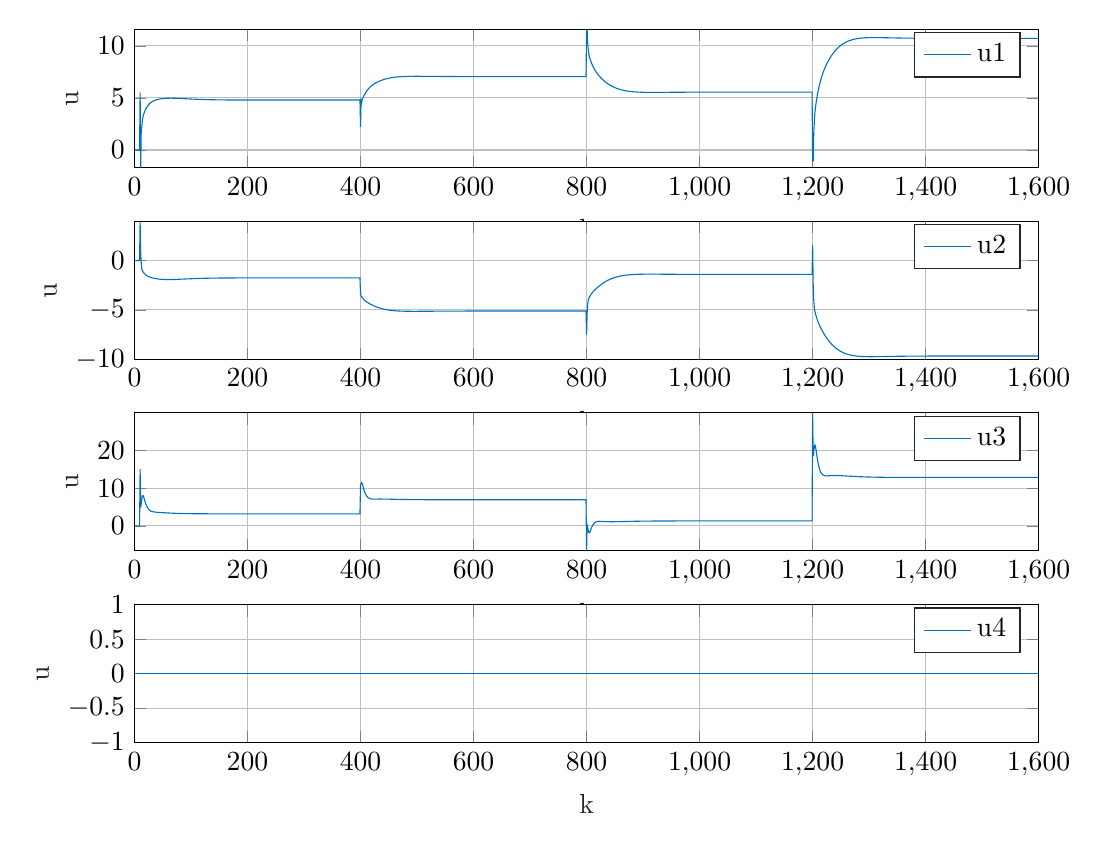
\begin{tikzpicture}

\begin{axis}[%
width=4.521in,
height=0.69in,
at={(0.758in,3.357in)},
scale only axis,
xmin=0,
xmax=1600,
xlabel style={font=\color{white!15!black}},
xlabel={k},
ymin=-1.6818,
ymax=11.563,
ylabel style={font=\color{white!15!black}},
ylabel={u},
axis background/.style={fill=white},
xmajorgrids,
ymajorgrids,
legend style={legend cell align=left, align=left, draw=white!15!black}
]
\addplot [color=mycolor1]
  table[row sep=crcr]{%
1	0\\
2	0\\
3	0\\
4	0\\
5	0\\
6	0\\
7	0\\
8	0\\
9	0\\
10	5.523\\
11	-1.6818\\
12	1.9732\\
13	2.1748\\
14	2.8907\\
15	3.16\\
16	3.3847\\
17	3.5451\\
18	3.6876\\
19	3.8146\\
20	3.9295\\
21	4.0327\\
22	4.1251\\
23	4.2077\\
24	4.2816\\
25	4.3479\\
26	4.4075\\
27	4.4611\\
28	4.5093\\
29	4.5529\\
30	4.5922\\
31	4.6279\\
32	4.6602\\
33	4.6896\\
34	4.7163\\
35	4.7407\\
36	4.763\\
37	4.7834\\
38	4.802\\
39	4.8192\\
40	4.8349\\
41	4.8494\\
42	4.8626\\
43	4.8748\\
44	4.886\\
45	4.8963\\
46	4.9057\\
47	4.9142\\
48	4.9221\\
49	4.9292\\
50	4.9356\\
51	4.9414\\
52	4.9466\\
53	4.9513\\
54	4.9554\\
55	4.959\\
56	4.9621\\
57	4.9648\\
58	4.967\\
59	4.9689\\
60	4.9704\\
61	4.9715\\
62	4.9723\\
63	4.9728\\
64	4.9729\\
65	4.9728\\
66	4.9725\\
67	4.9719\\
68	4.9711\\
69	4.97\\
70	4.9688\\
71	4.9674\\
72	4.9658\\
73	4.9641\\
74	4.9623\\
75	4.9603\\
76	4.9582\\
77	4.956\\
78	4.9537\\
79	4.9513\\
80	4.9488\\
81	4.9463\\
82	4.9437\\
83	4.9411\\
84	4.9384\\
85	4.9357\\
86	4.933\\
87	4.9302\\
88	4.9274\\
89	4.9246\\
90	4.9218\\
91	4.919\\
92	4.9162\\
93	4.9134\\
94	4.9106\\
95	4.9078\\
96	4.9051\\
97	4.9023\\
98	4.8996\\
99	4.8969\\
100	4.8942\\
101	4.8916\\
102	4.889\\
103	4.8864\\
104	4.8839\\
105	4.8814\\
106	4.8789\\
107	4.8765\\
108	4.8741\\
109	4.8718\\
110	4.8695\\
111	4.8672\\
112	4.865\\
113	4.8629\\
114	4.8607\\
115	4.8587\\
116	4.8566\\
117	4.8546\\
118	4.8527\\
119	4.8508\\
120	4.8489\\
121	4.8471\\
122	4.8453\\
123	4.8436\\
124	4.8419\\
125	4.8402\\
126	4.8386\\
127	4.8371\\
128	4.8356\\
129	4.8341\\
130	4.8326\\
131	4.8312\\
132	4.8299\\
133	4.8286\\
134	4.8273\\
135	4.826\\
136	4.8248\\
137	4.8237\\
138	4.8225\\
139	4.8214\\
140	4.8203\\
141	4.8193\\
142	4.8183\\
143	4.8173\\
144	4.8164\\
145	4.8155\\
146	4.8146\\
147	4.8138\\
148	4.8129\\
149	4.8122\\
150	4.8114\\
151	4.8106\\
152	4.8099\\
153	4.8092\\
154	4.8086\\
155	4.8079\\
156	4.8073\\
157	4.8067\\
158	4.8062\\
159	4.8056\\
160	4.8051\\
161	4.8046\\
162	4.8041\\
163	4.8036\\
164	4.8031\\
165	4.8027\\
166	4.8023\\
167	4.8019\\
168	4.8015\\
169	4.8011\\
170	4.8008\\
171	4.8004\\
172	4.8001\\
173	4.7998\\
174	4.7995\\
175	4.7992\\
176	4.7989\\
177	4.7987\\
178	4.7984\\
179	4.7982\\
180	4.798\\
181	4.7977\\
182	4.7975\\
183	4.7973\\
184	4.7971\\
185	4.797\\
186	4.7968\\
187	4.7966\\
188	4.7965\\
189	4.7963\\
190	4.7962\\
191	4.7961\\
192	4.7959\\
193	4.7958\\
194	4.7957\\
195	4.7956\\
196	4.7955\\
197	4.7954\\
198	4.7953\\
199	4.7952\\
200	4.7951\\
201	4.7951\\
202	4.795\\
203	4.7949\\
204	4.7949\\
205	4.7948\\
206	4.7947\\
207	4.7947\\
208	4.7946\\
209	4.7946\\
210	4.7946\\
211	4.7945\\
212	4.7945\\
213	4.7944\\
214	4.7944\\
215	4.7944\\
216	4.7944\\
217	4.7943\\
218	4.7943\\
219	4.7943\\
220	4.7943\\
221	4.7943\\
222	4.7942\\
223	4.7942\\
224	4.7942\\
225	4.7942\\
226	4.7942\\
227	4.7942\\
228	4.7942\\
229	4.7942\\
230	4.7942\\
231	4.7942\\
232	4.7942\\
233	4.7942\\
234	4.7942\\
235	4.7942\\
236	4.7942\\
237	4.7942\\
238	4.7942\\
239	4.7942\\
240	4.7942\\
241	4.7942\\
242	4.7942\\
243	4.7942\\
244	4.7942\\
245	4.7942\\
246	4.7942\\
247	4.7942\\
248	4.7942\\
249	4.7942\\
250	4.7942\\
251	4.7942\\
252	4.7942\\
253	4.7942\\
254	4.7942\\
255	4.7943\\
256	4.7943\\
257	4.7943\\
258	4.7943\\
259	4.7943\\
260	4.7943\\
261	4.7943\\
262	4.7943\\
263	4.7943\\
264	4.7943\\
265	4.7943\\
266	4.7943\\
267	4.7943\\
268	4.7943\\
269	4.7944\\
270	4.7944\\
271	4.7944\\
272	4.7944\\
273	4.7944\\
274	4.7944\\
275	4.7944\\
276	4.7944\\
277	4.7944\\
278	4.7944\\
279	4.7944\\
280	4.7944\\
281	4.7944\\
282	4.7944\\
283	4.7944\\
284	4.7944\\
285	4.7945\\
286	4.7945\\
287	4.7945\\
288	4.7945\\
289	4.7945\\
290	4.7945\\
291	4.7945\\
292	4.7945\\
293	4.7945\\
294	4.7945\\
295	4.7945\\
296	4.7945\\
297	4.7945\\
298	4.7945\\
299	4.7945\\
300	4.7945\\
301	4.7945\\
302	4.7945\\
303	4.7945\\
304	4.7945\\
305	4.7945\\
306	4.7945\\
307	4.7945\\
308	4.7945\\
309	4.7946\\
310	4.7946\\
311	4.7946\\
312	4.7946\\
313	4.7946\\
314	4.7946\\
315	4.7946\\
316	4.7946\\
317	4.7946\\
318	4.7946\\
319	4.7946\\
320	4.7946\\
321	4.7946\\
322	4.7946\\
323	4.7946\\
324	4.7946\\
325	4.7946\\
326	4.7946\\
327	4.7946\\
328	4.7946\\
329	4.7946\\
330	4.7946\\
331	4.7946\\
332	4.7946\\
333	4.7946\\
334	4.7946\\
335	4.7946\\
336	4.7946\\
337	4.7946\\
338	4.7946\\
339	4.7946\\
340	4.7946\\
341	4.7946\\
342	4.7946\\
343	4.7946\\
344	4.7946\\
345	4.7946\\
346	4.7946\\
347	4.7946\\
348	4.7946\\
349	4.7946\\
350	4.7946\\
351	4.7946\\
352	4.7946\\
353	4.7946\\
354	4.7946\\
355	4.7946\\
356	4.7946\\
357	4.7946\\
358	4.7946\\
359	4.7946\\
360	4.7946\\
361	4.7946\\
362	4.7946\\
363	4.7946\\
364	4.7946\\
365	4.7946\\
366	4.7946\\
367	4.7946\\
368	4.7946\\
369	4.7946\\
370	4.7946\\
371	4.7946\\
372	4.7946\\
373	4.7946\\
374	4.7946\\
375	4.7946\\
376	4.7946\\
377	4.7946\\
378	4.7946\\
379	4.7946\\
380	4.7946\\
381	4.7946\\
382	4.7946\\
383	4.7946\\
384	4.7946\\
385	4.7946\\
386	4.7946\\
387	4.7946\\
388	4.7946\\
389	4.7946\\
390	4.7946\\
391	4.7946\\
392	4.7946\\
393	4.7946\\
394	4.7946\\
395	4.7946\\
396	4.7946\\
397	4.7946\\
398	4.7946\\
399	4.7946\\
400	2.2172\\
401	4.7584\\
402	4.5838\\
403	4.8792\\
404	4.9727\\
405	5.0953\\
406	5.2024\\
407	5.3083\\
408	5.4076\\
409	5.5007\\
410	5.5871\\
411	5.6672\\
412	5.7416\\
413	5.8107\\
414	5.8751\\
415	5.9351\\
416	5.9912\\
417	6.0437\\
418	6.0931\\
419	6.1395\\
420	6.1834\\
421	6.2249\\
422	6.2643\\
423	6.3017\\
424	6.3374\\
425	6.3714\\
426	6.4039\\
427	6.435\\
428	6.4649\\
429	6.4935\\
430	6.521\\
431	6.5474\\
432	6.5727\\
433	6.5971\\
434	6.6205\\
435	6.643\\
436	6.6646\\
437	6.6853\\
438	6.7052\\
439	6.7244\\
440	6.7427\\
441	6.7603\\
442	6.7772\\
443	6.7933\\
444	6.8088\\
445	6.8236\\
446	6.8378\\
447	6.8513\\
448	6.8642\\
449	6.8766\\
450	6.8884\\
451	6.8996\\
452	6.9103\\
453	6.9205\\
454	6.9302\\
455	6.9394\\
456	6.9482\\
457	6.9565\\
458	6.9644\\
459	6.9719\\
460	6.979\\
461	6.9857\\
462	6.992\\
463	6.998\\
464	7.0037\\
465	7.0091\\
466	7.0141\\
467	7.0189\\
468	7.0233\\
469	7.0275\\
470	7.0315\\
471	7.0352\\
472	7.0386\\
473	7.0419\\
474	7.0449\\
475	7.0477\\
476	7.0503\\
477	7.0528\\
478	7.055\\
479	7.0571\\
480	7.059\\
481	7.0608\\
482	7.0624\\
483	7.0639\\
484	7.0653\\
485	7.0665\\
486	7.0677\\
487	7.0687\\
488	7.0696\\
489	7.0704\\
490	7.0711\\
491	7.0717\\
492	7.0723\\
493	7.0727\\
494	7.0731\\
495	7.0734\\
496	7.0737\\
497	7.0739\\
498	7.074\\
499	7.0741\\
500	7.0741\\
501	7.0741\\
502	7.074\\
503	7.0739\\
504	7.0738\\
505	7.0736\\
506	7.0734\\
507	7.0731\\
508	7.0729\\
509	7.0726\\
510	7.0723\\
511	7.0719\\
512	7.0716\\
513	7.0712\\
514	7.0708\\
515	7.0704\\
516	7.07\\
517	7.0696\\
518	7.0691\\
519	7.0687\\
520	7.0682\\
521	7.0678\\
522	7.0673\\
523	7.0668\\
524	7.0664\\
525	7.0659\\
526	7.0654\\
527	7.065\\
528	7.0645\\
529	7.064\\
530	7.0636\\
531	7.0631\\
532	7.0626\\
533	7.0622\\
534	7.0617\\
535	7.0612\\
536	7.0608\\
537	7.0604\\
538	7.0599\\
539	7.0595\\
540	7.0591\\
541	7.0586\\
542	7.0582\\
543	7.0578\\
544	7.0574\\
545	7.057\\
546	7.0566\\
547	7.0563\\
548	7.0559\\
549	7.0555\\
550	7.0552\\
551	7.0548\\
552	7.0545\\
553	7.0541\\
554	7.0538\\
555	7.0535\\
556	7.0532\\
557	7.0529\\
558	7.0526\\
559	7.0523\\
560	7.052\\
561	7.0517\\
562	7.0515\\
563	7.0512\\
564	7.0509\\
565	7.0507\\
566	7.0505\\
567	7.0502\\
568	7.05\\
569	7.0498\\
570	7.0496\\
571	7.0493\\
572	7.0491\\
573	7.0489\\
574	7.0488\\
575	7.0486\\
576	7.0484\\
577	7.0482\\
578	7.048\\
579	7.0479\\
580	7.0477\\
581	7.0476\\
582	7.0474\\
583	7.0473\\
584	7.0471\\
585	7.047\\
586	7.0469\\
587	7.0468\\
588	7.0466\\
589	7.0465\\
590	7.0464\\
591	7.0463\\
592	7.0462\\
593	7.0461\\
594	7.046\\
595	7.0459\\
596	7.0458\\
597	7.0457\\
598	7.0457\\
599	7.0456\\
600	7.0455\\
601	7.0454\\
602	7.0454\\
603	7.0453\\
604	7.0452\\
605	7.0452\\
606	7.0451\\
607	7.045\\
608	7.045\\
609	7.0449\\
610	7.0449\\
611	7.0448\\
612	7.0448\\
613	7.0447\\
614	7.0447\\
615	7.0447\\
616	7.0446\\
617	7.0446\\
618	7.0446\\
619	7.0445\\
620	7.0445\\
621	7.0445\\
622	7.0444\\
623	7.0444\\
624	7.0444\\
625	7.0444\\
626	7.0443\\
627	7.0443\\
628	7.0443\\
629	7.0443\\
630	7.0442\\
631	7.0442\\
632	7.0442\\
633	7.0442\\
634	7.0442\\
635	7.0442\\
636	7.0442\\
637	7.0441\\
638	7.0441\\
639	7.0441\\
640	7.0441\\
641	7.0441\\
642	7.0441\\
643	7.0441\\
644	7.0441\\
645	7.0441\\
646	7.0441\\
647	7.044\\
648	7.044\\
649	7.044\\
650	7.044\\
651	7.044\\
652	7.044\\
653	7.044\\
654	7.044\\
655	7.044\\
656	7.044\\
657	7.044\\
658	7.044\\
659	7.044\\
660	7.044\\
661	7.044\\
662	7.044\\
663	7.044\\
664	7.044\\
665	7.044\\
666	7.044\\
667	7.044\\
668	7.044\\
669	7.044\\
670	7.044\\
671	7.044\\
672	7.044\\
673	7.044\\
674	7.044\\
675	7.044\\
676	7.044\\
677	7.044\\
678	7.044\\
679	7.044\\
680	7.044\\
681	7.044\\
682	7.044\\
683	7.044\\
684	7.044\\
685	7.044\\
686	7.044\\
687	7.044\\
688	7.044\\
689	7.044\\
690	7.044\\
691	7.044\\
692	7.044\\
693	7.044\\
694	7.044\\
695	7.044\\
696	7.044\\
697	7.044\\
698	7.044\\
699	7.044\\
700	7.044\\
701	7.044\\
702	7.044\\
703	7.044\\
704	7.044\\
705	7.044\\
706	7.044\\
707	7.044\\
708	7.044\\
709	7.044\\
710	7.044\\
711	7.044\\
712	7.044\\
713	7.044\\
714	7.044\\
715	7.044\\
716	7.044\\
717	7.044\\
718	7.044\\
719	7.044\\
720	7.044\\
721	7.044\\
722	7.044\\
723	7.044\\
724	7.044\\
725	7.044\\
726	7.044\\
727	7.044\\
728	7.044\\
729	7.044\\
730	7.044\\
731	7.044\\
732	7.044\\
733	7.044\\
734	7.044\\
735	7.044\\
736	7.044\\
737	7.044\\
738	7.044\\
739	7.044\\
740	7.044\\
741	7.044\\
742	7.044\\
743	7.044\\
744	7.0441\\
745	7.0441\\
746	7.0441\\
747	7.0441\\
748	7.0441\\
749	7.0441\\
750	7.0441\\
751	7.0441\\
752	7.0441\\
753	7.0441\\
754	7.0441\\
755	7.0441\\
756	7.0441\\
757	7.0441\\
758	7.0441\\
759	7.0441\\
760	7.0441\\
761	7.0441\\
762	7.0441\\
763	7.0441\\
764	7.0441\\
765	7.0441\\
766	7.0441\\
767	7.0441\\
768	7.0441\\
769	7.0441\\
770	7.0441\\
771	7.0441\\
772	7.0441\\
773	7.0441\\
774	7.0441\\
775	7.0441\\
776	7.0441\\
777	7.0441\\
778	7.0441\\
779	7.0441\\
780	7.0441\\
781	7.0441\\
782	7.0441\\
783	7.0441\\
784	7.0441\\
785	7.0441\\
786	7.0441\\
787	7.0441\\
788	7.0441\\
789	7.0441\\
790	7.0441\\
791	7.0441\\
792	7.0441\\
793	7.0441\\
794	7.0441\\
795	7.0441\\
796	7.0441\\
797	7.0441\\
798	7.0441\\
799	7.0441\\
800	11.462\\
801	11.563\\
802	10.195\\
803	9.6649\\
804	9.2081\\
805	8.9508\\
806	8.7551\\
807	8.5949\\
808	8.4485\\
809	8.3119\\
810	8.1837\\
811	8.0637\\
812	7.9515\\
813	7.8464\\
814	7.7477\\
815	7.6547\\
816	7.5669\\
817	7.4837\\
818	7.4047\\
819	7.3296\\
820	7.258\\
821	7.1895\\
822	7.1239\\
823	7.0611\\
824	7.0006\\
825	6.9425\\
826	6.8865\\
827	6.8326\\
828	6.7805\\
829	6.7302\\
830	6.6815\\
831	6.6346\\
832	6.5891\\
833	6.5452\\
834	6.5027\\
835	6.4616\\
836	6.4219\\
837	6.3836\\
838	6.3465\\
839	6.3107\\
840	6.2761\\
841	6.2427\\
842	6.2105\\
843	6.1794\\
844	6.1495\\
845	6.1206\\
846	6.0928\\
847	6.0661\\
848	6.0403\\
849	6.0155\\
850	5.9917\\
851	5.9688\\
852	5.9469\\
853	5.9258\\
854	5.9055\\
855	5.8861\\
856	5.8675\\
857	5.8496\\
858	5.8326\\
859	5.8162\\
860	5.8006\\
861	5.7856\\
862	5.7713\\
863	5.7576\\
864	5.7445\\
865	5.7321\\
866	5.7202\\
867	5.7089\\
868	5.6981\\
869	5.6878\\
870	5.678\\
871	5.6686\\
872	5.6598\\
873	5.6514\\
874	5.6434\\
875	5.6358\\
876	5.6286\\
877	5.6218\\
878	5.6153\\
879	5.6092\\
880	5.6034\\
881	5.598\\
882	5.5928\\
883	5.5879\\
884	5.5834\\
885	5.579\\
886	5.575\\
887	5.5712\\
888	5.5676\\
889	5.5642\\
890	5.5611\\
891	5.5582\\
892	5.5554\\
893	5.5529\\
894	5.5505\\
895	5.5483\\
896	5.5462\\
897	5.5444\\
898	5.5426\\
899	5.541\\
900	5.5395\\
901	5.5382\\
902	5.5369\\
903	5.5358\\
904	5.5348\\
905	5.5339\\
906	5.5331\\
907	5.5323\\
908	5.5317\\
909	5.5311\\
910	5.5307\\
911	5.5302\\
912	5.5299\\
913	5.5296\\
914	5.5294\\
915	5.5292\\
916	5.5291\\
917	5.529\\
918	5.529\\
919	5.529\\
920	5.5291\\
921	5.5292\\
922	5.5293\\
923	5.5295\\
924	5.5297\\
925	5.5299\\
926	5.5302\\
927	5.5304\\
928	5.5307\\
929	5.531\\
930	5.5313\\
931	5.5317\\
932	5.532\\
933	5.5324\\
934	5.5328\\
935	5.5332\\
936	5.5336\\
937	5.534\\
938	5.5344\\
939	5.5348\\
940	5.5352\\
941	5.5357\\
942	5.5361\\
943	5.5365\\
944	5.5369\\
945	5.5374\\
946	5.5378\\
947	5.5382\\
948	5.5387\\
949	5.5391\\
950	5.5395\\
951	5.5399\\
952	5.5403\\
953	5.5408\\
954	5.5412\\
955	5.5416\\
956	5.542\\
957	5.5424\\
958	5.5427\\
959	5.5431\\
960	5.5435\\
961	5.5439\\
962	5.5442\\
963	5.5446\\
964	5.545\\
965	5.5453\\
966	5.5456\\
967	5.546\\
968	5.5463\\
969	5.5466\\
970	5.5469\\
971	5.5472\\
972	5.5475\\
973	5.5478\\
974	5.5481\\
975	5.5484\\
976	5.5486\\
977	5.5489\\
978	5.5492\\
979	5.5494\\
980	5.5497\\
981	5.5499\\
982	5.5501\\
983	5.5504\\
984	5.5506\\
985	5.5508\\
986	5.551\\
987	5.5512\\
988	5.5514\\
989	5.5516\\
990	5.5518\\
991	5.552\\
992	5.5521\\
993	5.5523\\
994	5.5525\\
995	5.5526\\
996	5.5528\\
997	5.5529\\
998	5.5531\\
999	5.5532\\
1000	5.5533\\
1001	5.5535\\
1002	5.5536\\
1003	5.5537\\
1004	5.5538\\
1005	5.5539\\
1006	5.554\\
1007	5.5542\\
1008	5.5543\\
1009	5.5544\\
1010	5.5544\\
1011	5.5545\\
1012	5.5546\\
1013	5.5547\\
1014	5.5548\\
1015	5.5549\\
1016	5.5549\\
1017	5.555\\
1018	5.5551\\
1019	5.5552\\
1020	5.5552\\
1021	5.5553\\
1022	5.5553\\
1023	5.5554\\
1024	5.5554\\
1025	5.5555\\
1026	5.5555\\
1027	5.5556\\
1028	5.5556\\
1029	5.5557\\
1030	5.5557\\
1031	5.5558\\
1032	5.5558\\
1033	5.5558\\
1034	5.5559\\
1035	5.5559\\
1036	5.5559\\
1037	5.556\\
1038	5.556\\
1039	5.556\\
1040	5.5561\\
1041	5.5561\\
1042	5.5561\\
1043	5.5561\\
1044	5.5561\\
1045	5.5562\\
1046	5.5562\\
1047	5.5562\\
1048	5.5562\\
1049	5.5562\\
1050	5.5563\\
1051	5.5563\\
1052	5.5563\\
1053	5.5563\\
1054	5.5563\\
1055	5.5563\\
1056	5.5563\\
1057	5.5563\\
1058	5.5563\\
1059	5.5564\\
1060	5.5564\\
1061	5.5564\\
1062	5.5564\\
1063	5.5564\\
1064	5.5564\\
1065	5.5564\\
1066	5.5564\\
1067	5.5564\\
1068	5.5564\\
1069	5.5564\\
1070	5.5564\\
1071	5.5564\\
1072	5.5564\\
1073	5.5564\\
1074	5.5564\\
1075	5.5564\\
1076	5.5564\\
1077	5.5564\\
1078	5.5564\\
1079	5.5564\\
1080	5.5565\\
1081	5.5565\\
1082	5.5565\\
1083	5.5565\\
1084	5.5565\\
1085	5.5565\\
1086	5.5565\\
1087	5.5565\\
1088	5.5565\\
1089	5.5565\\
1090	5.5565\\
1091	5.5565\\
1092	5.5565\\
1093	5.5565\\
1094	5.5565\\
1095	5.5565\\
1096	5.5565\\
1097	5.5565\\
1098	5.5565\\
1099	5.5565\\
1100	5.5565\\
1101	5.5564\\
1102	5.5564\\
1103	5.5564\\
1104	5.5564\\
1105	5.5564\\
1106	5.5564\\
1107	5.5564\\
1108	5.5564\\
1109	5.5564\\
1110	5.5564\\
1111	5.5564\\
1112	5.5564\\
1113	5.5564\\
1114	5.5564\\
1115	5.5564\\
1116	5.5564\\
1117	5.5564\\
1118	5.5564\\
1119	5.5564\\
1120	5.5564\\
1121	5.5564\\
1122	5.5564\\
1123	5.5564\\
1124	5.5564\\
1125	5.5564\\
1126	5.5564\\
1127	5.5564\\
1128	5.5564\\
1129	5.5564\\
1130	5.5564\\
1131	5.5564\\
1132	5.5564\\
1133	5.5564\\
1134	5.5564\\
1135	5.5564\\
1136	5.5564\\
1137	5.5564\\
1138	5.5564\\
1139	5.5564\\
1140	5.5564\\
1141	5.5564\\
1142	5.5564\\
1143	5.5564\\
1144	5.5564\\
1145	5.5564\\
1146	5.5564\\
1147	5.5564\\
1148	5.5564\\
1149	5.5564\\
1150	5.5564\\
1151	5.5564\\
1152	5.5564\\
1153	5.5564\\
1154	5.5564\\
1155	5.5564\\
1156	5.5564\\
1157	5.5564\\
1158	5.5564\\
1159	5.5564\\
1160	5.5564\\
1161	5.5564\\
1162	5.5564\\
1163	5.5564\\
1164	5.5564\\
1165	5.5564\\
1166	5.5564\\
1167	5.5564\\
1168	5.5564\\
1169	5.5564\\
1170	5.5564\\
1171	5.5564\\
1172	5.5564\\
1173	5.5564\\
1174	5.5564\\
1175	5.5564\\
1176	5.5564\\
1177	5.5564\\
1178	5.5564\\
1179	5.5564\\
1180	5.5564\\
1181	5.5564\\
1182	5.5564\\
1183	5.5564\\
1184	5.5564\\
1185	5.5564\\
1186	5.5564\\
1187	5.5564\\
1188	5.5564\\
1189	5.5564\\
1190	5.5564\\
1191	5.5564\\
1192	5.5564\\
1193	5.5564\\
1194	5.5564\\
1195	5.5564\\
1196	5.5564\\
1197	5.5564\\
1198	5.5564\\
1199	5.5564\\
1200	-1.0712\\
1201	-1.0419\\
1202	1.6471\\
1203	2.6631\\
1204	3.5509\\
1205	4.0728\\
1206	4.4865\\
1207	4.8339\\
1208	5.1525\\
1209	5.4484\\
1210	5.7242\\
1211	5.9805\\
1212	6.2187\\
1213	6.4403\\
1214	6.647\\
1215	6.8403\\
1216	7.0215\\
1217	7.1919\\
1218	7.3525\\
1219	7.5043\\
1220	7.6481\\
1221	7.7847\\
1222	7.9146\\
1223	8.0385\\
1224	8.1569\\
1225	8.2703\\
1226	8.3789\\
1227	8.4832\\
1228	8.5834\\
1229	8.6798\\
1230	8.7725\\
1231	8.8618\\
1232	8.9478\\
1233	9.0307\\
1234	9.1105\\
1235	9.1874\\
1236	9.2616\\
1237	9.333\\
1238	9.4017\\
1239	9.4679\\
1240	9.5316\\
1241	9.5929\\
1242	9.6518\\
1243	9.7085\\
1244	9.7629\\
1245	9.8152\\
1246	9.8654\\
1247	9.9135\\
1248	9.9596\\
1249	10.004\\
1250	10.046\\
1251	10.087\\
1252	10.126\\
1253	10.163\\
1254	10.198\\
1255	10.232\\
1256	10.264\\
1257	10.295\\
1258	10.325\\
1259	10.353\\
1260	10.379\\
1261	10.405\\
1262	10.429\\
1263	10.452\\
1264	10.474\\
1265	10.495\\
1266	10.514\\
1267	10.533\\
1268	10.551\\
1269	10.568\\
1270	10.583\\
1271	10.598\\
1272	10.613\\
1273	10.626\\
1274	10.639\\
1275	10.65\\
1276	10.662\\
1277	10.672\\
1278	10.682\\
1279	10.691\\
1280	10.7\\
1281	10.708\\
1282	10.716\\
1283	10.723\\
1284	10.729\\
1285	10.735\\
1286	10.741\\
1287	10.746\\
1288	10.751\\
1289	10.756\\
1290	10.76\\
1291	10.763\\
1292	10.767\\
1293	10.77\\
1294	10.773\\
1295	10.775\\
1296	10.778\\
1297	10.78\\
1298	10.782\\
1299	10.783\\
1300	10.785\\
1301	10.786\\
1302	10.787\\
1303	10.788\\
1304	10.788\\
1305	10.789\\
1306	10.789\\
1307	10.79\\
1308	10.79\\
1309	10.79\\
1310	10.79\\
1311	10.789\\
1312	10.789\\
1313	10.789\\
1314	10.788\\
1315	10.788\\
1316	10.787\\
1317	10.786\\
1318	10.786\\
1319	10.785\\
1320	10.784\\
1321	10.783\\
1322	10.782\\
1323	10.781\\
1324	10.78\\
1325	10.779\\
1326	10.778\\
1327	10.777\\
1328	10.776\\
1329	10.775\\
1330	10.774\\
1331	10.773\\
1332	10.772\\
1333	10.77\\
1334	10.769\\
1335	10.768\\
1336	10.767\\
1337	10.766\\
1338	10.765\\
1339	10.764\\
1340	10.762\\
1341	10.761\\
1342	10.76\\
1343	10.759\\
1344	10.758\\
1345	10.757\\
1346	10.756\\
1347	10.755\\
1348	10.754\\
1349	10.753\\
1350	10.752\\
1351	10.751\\
1352	10.75\\
1353	10.749\\
1354	10.748\\
1355	10.747\\
1356	10.746\\
1357	10.745\\
1358	10.744\\
1359	10.743\\
1360	10.743\\
1361	10.742\\
1362	10.741\\
1363	10.74\\
1364	10.739\\
1365	10.739\\
1366	10.738\\
1367	10.737\\
1368	10.737\\
1369	10.736\\
1370	10.735\\
1371	10.735\\
1372	10.734\\
1373	10.733\\
1374	10.733\\
1375	10.732\\
1376	10.732\\
1377	10.731\\
1378	10.731\\
1379	10.73\\
1380	10.729\\
1381	10.729\\
1382	10.729\\
1383	10.728\\
1384	10.728\\
1385	10.727\\
1386	10.727\\
1387	10.726\\
1388	10.726\\
1389	10.726\\
1390	10.725\\
1391	10.725\\
1392	10.725\\
1393	10.724\\
1394	10.724\\
1395	10.724\\
1396	10.723\\
1397	10.723\\
1398	10.723\\
1399	10.723\\
1400	10.722\\
1401	10.722\\
1402	10.722\\
1403	10.722\\
1404	10.721\\
1405	10.721\\
1406	10.721\\
1407	10.721\\
1408	10.721\\
1409	10.72\\
1410	10.72\\
1411	10.72\\
1412	10.72\\
1413	10.72\\
1414	10.72\\
1415	10.719\\
1416	10.719\\
1417	10.719\\
1418	10.719\\
1419	10.719\\
1420	10.719\\
1421	10.719\\
1422	10.719\\
1423	10.718\\
1424	10.718\\
1425	10.718\\
1426	10.718\\
1427	10.718\\
1428	10.718\\
1429	10.718\\
1430	10.718\\
1431	10.718\\
1432	10.718\\
1433	10.718\\
1434	10.718\\
1435	10.718\\
1436	10.718\\
1437	10.717\\
1438	10.717\\
1439	10.717\\
1440	10.717\\
1441	10.717\\
1442	10.717\\
1443	10.717\\
1444	10.717\\
1445	10.717\\
1446	10.717\\
1447	10.717\\
1448	10.717\\
1449	10.717\\
1450	10.717\\
1451	10.717\\
1452	10.717\\
1453	10.717\\
1454	10.717\\
1455	10.717\\
1456	10.717\\
1457	10.717\\
1458	10.717\\
1459	10.717\\
1460	10.717\\
1461	10.717\\
1462	10.717\\
1463	10.717\\
1464	10.717\\
1465	10.717\\
1466	10.717\\
1467	10.717\\
1468	10.717\\
1469	10.717\\
1470	10.717\\
1471	10.717\\
1472	10.717\\
1473	10.717\\
1474	10.717\\
1475	10.717\\
1476	10.717\\
1477	10.717\\
1478	10.717\\
1479	10.717\\
1480	10.717\\
1481	10.717\\
1482	10.717\\
1483	10.717\\
1484	10.717\\
1485	10.717\\
1486	10.717\\
1487	10.717\\
1488	10.717\\
1489	10.717\\
1490	10.717\\
1491	10.717\\
1492	10.717\\
1493	10.717\\
1494	10.717\\
1495	10.717\\
1496	10.717\\
1497	10.717\\
1498	10.717\\
1499	10.717\\
1500	10.717\\
1501	10.717\\
1502	10.717\\
1503	10.717\\
1504	10.717\\
1505	10.717\\
1506	10.717\\
1507	10.717\\
1508	10.717\\
1509	10.717\\
1510	10.717\\
1511	10.717\\
1512	10.717\\
1513	10.717\\
1514	10.717\\
1515	10.717\\
1516	10.717\\
1517	10.717\\
1518	10.717\\
1519	10.717\\
1520	10.717\\
1521	10.717\\
1522	10.717\\
1523	10.717\\
1524	10.717\\
1525	10.717\\
1526	10.717\\
1527	10.717\\
1528	10.717\\
1529	10.717\\
1530	10.717\\
1531	10.717\\
1532	10.717\\
1533	10.717\\
1534	10.717\\
1535	10.717\\
1536	10.717\\
1537	10.717\\
1538	10.717\\
1539	10.717\\
1540	10.717\\
1541	10.717\\
1542	10.717\\
1543	10.717\\
1544	10.717\\
1545	10.717\\
1546	10.717\\
1547	10.717\\
1548	10.717\\
1549	10.717\\
1550	10.717\\
1551	10.717\\
1552	10.717\\
1553	10.717\\
1554	10.717\\
1555	10.717\\
1556	10.717\\
1557	10.717\\
1558	10.717\\
1559	10.717\\
1560	10.717\\
1561	10.717\\
1562	10.717\\
1563	10.717\\
1564	10.717\\
1565	10.717\\
1566	10.717\\
1567	10.717\\
1568	10.717\\
1569	10.717\\
1570	10.717\\
1571	10.717\\
1572	10.717\\
1573	10.717\\
1574	10.717\\
1575	10.717\\
1576	10.717\\
1577	10.717\\
1578	10.717\\
1579	10.717\\
1580	10.717\\
1581	10.717\\
1582	10.717\\
1583	10.717\\
1584	10.717\\
1585	10.717\\
1586	10.717\\
1587	10.717\\
1588	10.717\\
1589	10.717\\
1590	10.717\\
1591	10.717\\
1592	10.717\\
1593	10.717\\
1594	10.717\\
1595	10.717\\
1596	10.717\\
1597	10.717\\
1598	10.717\\
1599	10.717\\
1600	10.717\\
};
\addlegendentry{u1}

\end{axis}

\begin{axis}[%
width=4.521in,
height=0.69in,
at={(0.758in,2.398in)},
scale only axis,
xmin=0,
xmax=1600,
xlabel style={font=\color{white!15!black}},
xlabel={k},
ymin=-10,
ymax=3.9647,
ylabel style={font=\color{white!15!black}},
ylabel={u},
axis background/.style={fill=white},
xmajorgrids,
ymajorgrids,
legend style={legend cell align=left, align=left, draw=white!15!black}
]
\addplot [color=mycolor1]
  table[row sep=crcr]{%
1	0\\
2	0\\
3	0\\
4	0\\
5	0\\
6	0\\
7	0\\
8	0\\
9	0\\
10	3.9647\\
11	0.81725\\
12	-0.29254\\
13	-0.84603\\
14	-1.0378\\
15	-1.1347\\
16	-1.2069\\
17	-1.2778\\
18	-1.3454\\
19	-1.4062\\
20	-1.4586\\
21	-1.5031\\
22	-1.5411\\
23	-1.5741\\
24	-1.6032\\
25	-1.6293\\
26	-1.653\\
27	-1.6748\\
28	-1.6949\\
29	-1.7137\\
30	-1.7313\\
31	-1.7479\\
32	-1.7634\\
33	-1.778\\
34	-1.7917\\
35	-1.8047\\
36	-1.8168\\
37	-1.8282\\
38	-1.8388\\
39	-1.8487\\
40	-1.8579\\
41	-1.8665\\
42	-1.8744\\
43	-1.8817\\
44	-1.8883\\
45	-1.8944\\
46	-1.8999\\
47	-1.9049\\
48	-1.9093\\
49	-1.9133\\
50	-1.9168\\
51	-1.9198\\
52	-1.9224\\
53	-1.9247\\
54	-1.9265\\
55	-1.9279\\
56	-1.9291\\
57	-1.9298\\
58	-1.9303\\
59	-1.9305\\
60	-1.9305\\
61	-1.9302\\
62	-1.9296\\
63	-1.9289\\
64	-1.9279\\
65	-1.9268\\
66	-1.9255\\
67	-1.924\\
68	-1.9224\\
69	-1.9206\\
70	-1.9188\\
71	-1.9168\\
72	-1.9147\\
73	-1.9125\\
74	-1.9103\\
75	-1.908\\
76	-1.9056\\
77	-1.9031\\
78	-1.9006\\
79	-1.8981\\
80	-1.8956\\
81	-1.893\\
82	-1.8903\\
83	-1.8877\\
84	-1.8851\\
85	-1.8824\\
86	-1.8798\\
87	-1.8771\\
88	-1.8745\\
89	-1.8718\\
90	-1.8692\\
91	-1.8666\\
92	-1.864\\
93	-1.8615\\
94	-1.8589\\
95	-1.8564\\
96	-1.8539\\
97	-1.8515\\
98	-1.849\\
99	-1.8466\\
100	-1.8443\\
101	-1.842\\
102	-1.8397\\
103	-1.8374\\
104	-1.8352\\
105	-1.8331\\
106	-1.8309\\
107	-1.8288\\
108	-1.8268\\
109	-1.8248\\
110	-1.8228\\
111	-1.8209\\
112	-1.819\\
113	-1.8172\\
114	-1.8154\\
115	-1.8136\\
116	-1.8119\\
117	-1.8102\\
118	-1.8086\\
119	-1.807\\
120	-1.8055\\
121	-1.804\\
122	-1.8025\\
123	-1.801\\
124	-1.7997\\
125	-1.7983\\
126	-1.797\\
127	-1.7957\\
128	-1.7945\\
129	-1.7932\\
130	-1.7921\\
131	-1.7909\\
132	-1.7898\\
133	-1.7888\\
134	-1.7877\\
135	-1.7867\\
136	-1.7857\\
137	-1.7848\\
138	-1.7839\\
139	-1.783\\
140	-1.7821\\
141	-1.7813\\
142	-1.7805\\
143	-1.7797\\
144	-1.779\\
145	-1.7783\\
146	-1.7776\\
147	-1.7769\\
148	-1.7763\\
149	-1.7756\\
150	-1.775\\
151	-1.7745\\
152	-1.7739\\
153	-1.7734\\
154	-1.7728\\
155	-1.7723\\
156	-1.7719\\
157	-1.7714\\
158	-1.7709\\
159	-1.7705\\
160	-1.7701\\
161	-1.7697\\
162	-1.7693\\
163	-1.769\\
164	-1.7686\\
165	-1.7683\\
166	-1.768\\
167	-1.7677\\
168	-1.7674\\
169	-1.7671\\
170	-1.7668\\
171	-1.7666\\
172	-1.7663\\
173	-1.7661\\
174	-1.7659\\
175	-1.7656\\
176	-1.7654\\
177	-1.7652\\
178	-1.7651\\
179	-1.7649\\
180	-1.7647\\
181	-1.7645\\
182	-1.7644\\
183	-1.7642\\
184	-1.7641\\
185	-1.764\\
186	-1.7639\\
187	-1.7637\\
188	-1.7636\\
189	-1.7635\\
190	-1.7634\\
191	-1.7633\\
192	-1.7632\\
193	-1.7631\\
194	-1.7631\\
195	-1.763\\
196	-1.7629\\
197	-1.7628\\
198	-1.7628\\
199	-1.7627\\
200	-1.7627\\
201	-1.7626\\
202	-1.7626\\
203	-1.7625\\
204	-1.7625\\
205	-1.7624\\
206	-1.7624\\
207	-1.7624\\
208	-1.7623\\
209	-1.7623\\
210	-1.7623\\
211	-1.7623\\
212	-1.7622\\
213	-1.7622\\
214	-1.7622\\
215	-1.7622\\
216	-1.7622\\
217	-1.7621\\
218	-1.7621\\
219	-1.7621\\
220	-1.7621\\
221	-1.7621\\
222	-1.7621\\
223	-1.7621\\
224	-1.7621\\
225	-1.7621\\
226	-1.7621\\
227	-1.7621\\
228	-1.7621\\
229	-1.7621\\
230	-1.7621\\
231	-1.7621\\
232	-1.7621\\
233	-1.7621\\
234	-1.7621\\
235	-1.7621\\
236	-1.7621\\
237	-1.7621\\
238	-1.7621\\
239	-1.7621\\
240	-1.7621\\
241	-1.7621\\
242	-1.7621\\
243	-1.7621\\
244	-1.7621\\
245	-1.7621\\
246	-1.7621\\
247	-1.7621\\
248	-1.7622\\
249	-1.7622\\
250	-1.7622\\
251	-1.7622\\
252	-1.7622\\
253	-1.7622\\
254	-1.7622\\
255	-1.7622\\
256	-1.7622\\
257	-1.7622\\
258	-1.7622\\
259	-1.7622\\
260	-1.7622\\
261	-1.7622\\
262	-1.7622\\
263	-1.7623\\
264	-1.7623\\
265	-1.7623\\
266	-1.7623\\
267	-1.7623\\
268	-1.7623\\
269	-1.7623\\
270	-1.7623\\
271	-1.7623\\
272	-1.7623\\
273	-1.7623\\
274	-1.7623\\
275	-1.7623\\
276	-1.7623\\
277	-1.7623\\
278	-1.7623\\
279	-1.7623\\
280	-1.7624\\
281	-1.7624\\
282	-1.7624\\
283	-1.7624\\
284	-1.7624\\
285	-1.7624\\
286	-1.7624\\
287	-1.7624\\
288	-1.7624\\
289	-1.7624\\
290	-1.7624\\
291	-1.7624\\
292	-1.7624\\
293	-1.7624\\
294	-1.7624\\
295	-1.7624\\
296	-1.7624\\
297	-1.7624\\
298	-1.7624\\
299	-1.7624\\
300	-1.7624\\
301	-1.7624\\
302	-1.7624\\
303	-1.7624\\
304	-1.7624\\
305	-1.7624\\
306	-1.7624\\
307	-1.7625\\
308	-1.7625\\
309	-1.7625\\
310	-1.7625\\
311	-1.7625\\
312	-1.7625\\
313	-1.7625\\
314	-1.7625\\
315	-1.7625\\
316	-1.7625\\
317	-1.7625\\
318	-1.7625\\
319	-1.7625\\
320	-1.7625\\
321	-1.7625\\
322	-1.7625\\
323	-1.7625\\
324	-1.7625\\
325	-1.7625\\
326	-1.7625\\
327	-1.7625\\
328	-1.7625\\
329	-1.7625\\
330	-1.7625\\
331	-1.7625\\
332	-1.7625\\
333	-1.7625\\
334	-1.7625\\
335	-1.7625\\
336	-1.7625\\
337	-1.7625\\
338	-1.7625\\
339	-1.7625\\
340	-1.7625\\
341	-1.7625\\
342	-1.7625\\
343	-1.7625\\
344	-1.7625\\
345	-1.7625\\
346	-1.7625\\
347	-1.7625\\
348	-1.7625\\
349	-1.7625\\
350	-1.7625\\
351	-1.7625\\
352	-1.7625\\
353	-1.7625\\
354	-1.7625\\
355	-1.7625\\
356	-1.7625\\
357	-1.7625\\
358	-1.7625\\
359	-1.7625\\
360	-1.7625\\
361	-1.7625\\
362	-1.7625\\
363	-1.7625\\
364	-1.7625\\
365	-1.7625\\
366	-1.7625\\
367	-1.7625\\
368	-1.7625\\
369	-1.7625\\
370	-1.7625\\
371	-1.7625\\
372	-1.7625\\
373	-1.7625\\
374	-1.7625\\
375	-1.7625\\
376	-1.7625\\
377	-1.7625\\
378	-1.7625\\
379	-1.7625\\
380	-1.7625\\
381	-1.7625\\
382	-1.7625\\
383	-1.7625\\
384	-1.7625\\
385	-1.7625\\
386	-1.7625\\
387	-1.7625\\
388	-1.7625\\
389	-1.7625\\
390	-1.7625\\
391	-1.7625\\
392	-1.7625\\
393	-1.7625\\
394	-1.7625\\
395	-1.7625\\
396	-1.7625\\
397	-1.7625\\
398	-1.7625\\
399	-1.7625\\
400	-3.3484\\
401	-3.5957\\
402	-3.6997\\
403	-3.7524\\
404	-3.8171\\
405	-3.8846\\
406	-3.9507\\
407	-4.0109\\
408	-4.0647\\
409	-4.1128\\
410	-4.1564\\
411	-4.1968\\
412	-4.2347\\
413	-4.2708\\
414	-4.3053\\
415	-4.3386\\
416	-4.3708\\
417	-4.402\\
418	-4.4324\\
419	-4.4619\\
420	-4.4907\\
421	-4.5186\\
422	-4.5458\\
423	-4.5722\\
424	-4.5978\\
425	-4.6226\\
426	-4.6467\\
427	-4.6699\\
428	-4.6924\\
429	-4.7142\\
430	-4.7351\\
431	-4.7554\\
432	-4.7748\\
433	-4.7936\\
434	-4.8116\\
435	-4.8289\\
436	-4.8455\\
437	-4.8614\\
438	-4.8767\\
439	-4.8913\\
440	-4.9053\\
441	-4.9187\\
442	-4.9315\\
443	-4.9437\\
444	-4.9554\\
445	-4.9665\\
446	-4.9771\\
447	-4.9872\\
448	-4.9968\\
449	-5.0059\\
450	-5.0146\\
451	-5.0229\\
452	-5.0307\\
453	-5.0382\\
454	-5.0452\\
455	-5.0519\\
456	-5.0582\\
457	-5.0642\\
458	-5.0699\\
459	-5.0752\\
460	-5.0802\\
461	-5.085\\
462	-5.0894\\
463	-5.0936\\
464	-5.0976\\
465	-5.1013\\
466	-5.1047\\
467	-5.108\\
468	-5.111\\
469	-5.1139\\
470	-5.1165\\
471	-5.119\\
472	-5.1212\\
473	-5.1234\\
474	-5.1253\\
475	-5.1271\\
476	-5.1288\\
477	-5.1303\\
478	-5.1317\\
479	-5.133\\
480	-5.1341\\
481	-5.1352\\
482	-5.1361\\
483	-5.137\\
484	-5.1377\\
485	-5.1384\\
486	-5.139\\
487	-5.1395\\
488	-5.1399\\
489	-5.1403\\
490	-5.1406\\
491	-5.1408\\
492	-5.141\\
493	-5.1411\\
494	-5.1411\\
495	-5.1412\\
496	-5.1411\\
497	-5.1411\\
498	-5.141\\
499	-5.1408\\
500	-5.1407\\
501	-5.1405\\
502	-5.1402\\
503	-5.14\\
504	-5.1397\\
505	-5.1394\\
506	-5.1391\\
507	-5.1387\\
508	-5.1384\\
509	-5.138\\
510	-5.1376\\
511	-5.1372\\
512	-5.1368\\
513	-5.1364\\
514	-5.136\\
515	-5.1356\\
516	-5.1351\\
517	-5.1347\\
518	-5.1343\\
519	-5.1338\\
520	-5.1334\\
521	-5.1329\\
522	-5.1325\\
523	-5.132\\
524	-5.1316\\
525	-5.1311\\
526	-5.1307\\
527	-5.1303\\
528	-5.1298\\
529	-5.1294\\
530	-5.129\\
531	-5.1285\\
532	-5.1281\\
533	-5.1277\\
534	-5.1273\\
535	-5.1269\\
536	-5.1265\\
537	-5.1261\\
538	-5.1257\\
539	-5.1254\\
540	-5.125\\
541	-5.1246\\
542	-5.1243\\
543	-5.1239\\
544	-5.1236\\
545	-5.1232\\
546	-5.1229\\
547	-5.1226\\
548	-5.1223\\
549	-5.122\\
550	-5.1217\\
551	-5.1214\\
552	-5.1211\\
553	-5.1208\\
554	-5.1205\\
555	-5.1203\\
556	-5.12\\
557	-5.1197\\
558	-5.1195\\
559	-5.1192\\
560	-5.119\\
561	-5.1188\\
562	-5.1186\\
563	-5.1184\\
564	-5.1181\\
565	-5.1179\\
566	-5.1177\\
567	-5.1176\\
568	-5.1174\\
569	-5.1172\\
570	-5.117\\
571	-5.1168\\
572	-5.1167\\
573	-5.1165\\
574	-5.1164\\
575	-5.1162\\
576	-5.1161\\
577	-5.1159\\
578	-5.1158\\
579	-5.1157\\
580	-5.1155\\
581	-5.1154\\
582	-5.1153\\
583	-5.1152\\
584	-5.1151\\
585	-5.115\\
586	-5.1149\\
587	-5.1148\\
588	-5.1147\\
589	-5.1146\\
590	-5.1145\\
591	-5.1144\\
592	-5.1143\\
593	-5.1143\\
594	-5.1142\\
595	-5.1141\\
596	-5.1141\\
597	-5.114\\
598	-5.1139\\
599	-5.1139\\
600	-5.1138\\
601	-5.1137\\
602	-5.1137\\
603	-5.1136\\
604	-5.1136\\
605	-5.1135\\
606	-5.1135\\
607	-5.1135\\
608	-5.1134\\
609	-5.1134\\
610	-5.1133\\
611	-5.1133\\
612	-5.1133\\
613	-5.1132\\
614	-5.1132\\
615	-5.1132\\
616	-5.1131\\
617	-5.1131\\
618	-5.1131\\
619	-5.1131\\
620	-5.113\\
621	-5.113\\
622	-5.113\\
623	-5.113\\
624	-5.113\\
625	-5.1129\\
626	-5.1129\\
627	-5.1129\\
628	-5.1129\\
629	-5.1129\\
630	-5.1129\\
631	-5.1129\\
632	-5.1128\\
633	-5.1128\\
634	-5.1128\\
635	-5.1128\\
636	-5.1128\\
637	-5.1128\\
638	-5.1128\\
639	-5.1128\\
640	-5.1128\\
641	-5.1128\\
642	-5.1128\\
643	-5.1127\\
644	-5.1127\\
645	-5.1127\\
646	-5.1127\\
647	-5.1127\\
648	-5.1127\\
649	-5.1127\\
650	-5.1127\\
651	-5.1127\\
652	-5.1127\\
653	-5.1127\\
654	-5.1127\\
655	-5.1127\\
656	-5.1127\\
657	-5.1127\\
658	-5.1127\\
659	-5.1127\\
660	-5.1127\\
661	-5.1127\\
662	-5.1127\\
663	-5.1127\\
664	-5.1127\\
665	-5.1127\\
666	-5.1127\\
667	-5.1127\\
668	-5.1127\\
669	-5.1127\\
670	-5.1127\\
671	-5.1127\\
672	-5.1127\\
673	-5.1127\\
674	-5.1127\\
675	-5.1127\\
676	-5.1127\\
677	-5.1127\\
678	-5.1127\\
679	-5.1127\\
680	-5.1127\\
681	-5.1127\\
682	-5.1127\\
683	-5.1127\\
684	-5.1127\\
685	-5.1127\\
686	-5.1127\\
687	-5.1127\\
688	-5.1127\\
689	-5.1127\\
690	-5.1127\\
691	-5.1127\\
692	-5.1127\\
693	-5.1127\\
694	-5.1127\\
695	-5.1127\\
696	-5.1127\\
697	-5.1127\\
698	-5.1127\\
699	-5.1127\\
700	-5.1127\\
701	-5.1127\\
702	-5.1127\\
703	-5.1127\\
704	-5.1127\\
705	-5.1127\\
706	-5.1127\\
707	-5.1127\\
708	-5.1127\\
709	-5.1127\\
710	-5.1127\\
711	-5.1127\\
712	-5.1127\\
713	-5.1127\\
714	-5.1127\\
715	-5.1127\\
716	-5.1127\\
717	-5.1127\\
718	-5.1127\\
719	-5.1127\\
720	-5.1127\\
721	-5.1127\\
722	-5.1127\\
723	-5.1127\\
724	-5.1128\\
725	-5.1128\\
726	-5.1128\\
727	-5.1128\\
728	-5.1128\\
729	-5.1128\\
730	-5.1128\\
731	-5.1128\\
732	-5.1128\\
733	-5.1128\\
734	-5.1128\\
735	-5.1128\\
736	-5.1128\\
737	-5.1128\\
738	-5.1128\\
739	-5.1128\\
740	-5.1128\\
741	-5.1128\\
742	-5.1128\\
743	-5.1128\\
744	-5.1128\\
745	-5.1128\\
746	-5.1128\\
747	-5.1128\\
748	-5.1128\\
749	-5.1128\\
750	-5.1128\\
751	-5.1128\\
752	-5.1128\\
753	-5.1128\\
754	-5.1128\\
755	-5.1128\\
756	-5.1128\\
757	-5.1128\\
758	-5.1128\\
759	-5.1128\\
760	-5.1128\\
761	-5.1128\\
762	-5.1128\\
763	-5.1128\\
764	-5.1128\\
765	-5.1128\\
766	-5.1128\\
767	-5.1128\\
768	-5.1128\\
769	-5.1128\\
770	-5.1128\\
771	-5.1128\\
772	-5.1128\\
773	-5.1128\\
774	-5.1128\\
775	-5.1128\\
776	-5.1128\\
777	-5.1128\\
778	-5.1128\\
779	-5.1128\\
780	-5.1128\\
781	-5.1128\\
782	-5.1128\\
783	-5.1128\\
784	-5.1128\\
785	-5.1128\\
786	-5.1128\\
787	-5.1128\\
788	-5.1128\\
789	-5.1128\\
790	-5.1128\\
791	-5.1128\\
792	-5.1128\\
793	-5.1128\\
794	-5.1128\\
795	-5.1128\\
796	-5.1128\\
797	-5.1128\\
798	-5.1128\\
799	-5.1128\\
800	-7.4916\\
801	-5.3164\\
802	-4.4167\\
803	-3.9959\\
804	-3.8147\\
805	-3.7061\\
806	-3.6134\\
807	-3.5222\\
808	-3.4336\\
809	-3.3503\\
810	-3.2733\\
811	-3.202\\
812	-3.1356\\
813	-3.0729\\
814	-3.0131\\
815	-2.9556\\
816	-2.9001\\
817	-2.8461\\
818	-2.7936\\
819	-2.7425\\
820	-2.6926\\
821	-2.6439\\
822	-2.5964\\
823	-2.55\\
824	-2.5049\\
825	-2.4608\\
826	-2.418\\
827	-2.3763\\
828	-2.3357\\
829	-2.2964\\
830	-2.2582\\
831	-2.2211\\
832	-2.1852\\
833	-2.1505\\
834	-2.1168\\
835	-2.0843\\
836	-2.0529\\
837	-2.0226\\
838	-1.9933\\
839	-1.9651\\
840	-1.9379\\
841	-1.9116\\
842	-1.8864\\
843	-1.8621\\
844	-1.8388\\
845	-1.8163\\
846	-1.7948\\
847	-1.774\\
848	-1.7542\\
849	-1.7351\\
850	-1.7168\\
851	-1.6992\\
852	-1.6824\\
853	-1.6664\\
854	-1.651\\
855	-1.6362\\
856	-1.6221\\
857	-1.6087\\
858	-1.5958\\
859	-1.5835\\
860	-1.5718\\
861	-1.5606\\
862	-1.55\\
863	-1.5398\\
864	-1.5301\\
865	-1.5209\\
866	-1.5122\\
867	-1.5038\\
868	-1.4959\\
869	-1.4884\\
870	-1.4813\\
871	-1.4745\\
872	-1.4681\\
873	-1.462\\
874	-1.4563\\
875	-1.4509\\
876	-1.4457\\
877	-1.4409\\
878	-1.4363\\
879	-1.432\\
880	-1.428\\
881	-1.4242\\
882	-1.4206\\
883	-1.4172\\
884	-1.4141\\
885	-1.4111\\
886	-1.4084\\
887	-1.4058\\
888	-1.4034\\
889	-1.4012\\
890	-1.3991\\
891	-1.3972\\
892	-1.3954\\
893	-1.3938\\
894	-1.3923\\
895	-1.3909\\
896	-1.3897\\
897	-1.3885\\
898	-1.3875\\
899	-1.3865\\
900	-1.3857\\
901	-1.3849\\
902	-1.3842\\
903	-1.3836\\
904	-1.3831\\
905	-1.3826\\
906	-1.3823\\
907	-1.3819\\
908	-1.3817\\
909	-1.3815\\
910	-1.3813\\
911	-1.3812\\
912	-1.3812\\
913	-1.3811\\
914	-1.3812\\
915	-1.3812\\
916	-1.3813\\
917	-1.3815\\
918	-1.3816\\
919	-1.3818\\
920	-1.382\\
921	-1.3822\\
922	-1.3825\\
923	-1.3828\\
924	-1.3831\\
925	-1.3834\\
926	-1.3837\\
927	-1.384\\
928	-1.3844\\
929	-1.3848\\
930	-1.3851\\
931	-1.3855\\
932	-1.3859\\
933	-1.3863\\
934	-1.3867\\
935	-1.3871\\
936	-1.3875\\
937	-1.3879\\
938	-1.3883\\
939	-1.3887\\
940	-1.3891\\
941	-1.3895\\
942	-1.3899\\
943	-1.3903\\
944	-1.3907\\
945	-1.3911\\
946	-1.3915\\
947	-1.3919\\
948	-1.3923\\
949	-1.3927\\
950	-1.3931\\
951	-1.3934\\
952	-1.3938\\
953	-1.3942\\
954	-1.3945\\
955	-1.3949\\
956	-1.3952\\
957	-1.3956\\
958	-1.3959\\
959	-1.3962\\
960	-1.3966\\
961	-1.3969\\
962	-1.3972\\
963	-1.3975\\
964	-1.3978\\
965	-1.3981\\
966	-1.3984\\
967	-1.3987\\
968	-1.3989\\
969	-1.3992\\
970	-1.3995\\
971	-1.3997\\
972	-1.4\\
973	-1.4002\\
974	-1.4005\\
975	-1.4007\\
976	-1.4009\\
977	-1.4011\\
978	-1.4013\\
979	-1.4016\\
980	-1.4018\\
981	-1.402\\
982	-1.4021\\
983	-1.4023\\
984	-1.4025\\
985	-1.4027\\
986	-1.4028\\
987	-1.403\\
988	-1.4032\\
989	-1.4033\\
990	-1.4035\\
991	-1.4036\\
992	-1.4038\\
993	-1.4039\\
994	-1.404\\
995	-1.4041\\
996	-1.4043\\
997	-1.4044\\
998	-1.4045\\
999	-1.4046\\
1000	-1.4047\\
1001	-1.4048\\
1002	-1.4049\\
1003	-1.405\\
1004	-1.4051\\
1005	-1.4052\\
1006	-1.4053\\
1007	-1.4054\\
1008	-1.4054\\
1009	-1.4055\\
1010	-1.4056\\
1011	-1.4057\\
1012	-1.4057\\
1013	-1.4058\\
1014	-1.4059\\
1015	-1.4059\\
1016	-1.406\\
1017	-1.406\\
1018	-1.4061\\
1019	-1.4061\\
1020	-1.4062\\
1021	-1.4062\\
1022	-1.4063\\
1023	-1.4063\\
1024	-1.4064\\
1025	-1.4064\\
1026	-1.4064\\
1027	-1.4065\\
1028	-1.4065\\
1029	-1.4065\\
1030	-1.4066\\
1031	-1.4066\\
1032	-1.4066\\
1033	-1.4067\\
1034	-1.4067\\
1035	-1.4067\\
1036	-1.4067\\
1037	-1.4068\\
1038	-1.4068\\
1039	-1.4068\\
1040	-1.4068\\
1041	-1.4068\\
1042	-1.4069\\
1043	-1.4069\\
1044	-1.4069\\
1045	-1.4069\\
1046	-1.4069\\
1047	-1.4069\\
1048	-1.4069\\
1049	-1.4069\\
1050	-1.407\\
1051	-1.407\\
1052	-1.407\\
1053	-1.407\\
1054	-1.407\\
1055	-1.407\\
1056	-1.407\\
1057	-1.407\\
1058	-1.407\\
1059	-1.407\\
1060	-1.407\\
1061	-1.407\\
1062	-1.407\\
1063	-1.4071\\
1064	-1.4071\\
1065	-1.4071\\
1066	-1.4071\\
1067	-1.4071\\
1068	-1.4071\\
1069	-1.4071\\
1070	-1.4071\\
1071	-1.4071\\
1072	-1.4071\\
1073	-1.4071\\
1074	-1.4071\\
1075	-1.4071\\
1076	-1.4071\\
1077	-1.4071\\
1078	-1.4071\\
1079	-1.4071\\
1080	-1.4071\\
1081	-1.4071\\
1082	-1.4071\\
1083	-1.4071\\
1084	-1.4071\\
1085	-1.4071\\
1086	-1.4071\\
1087	-1.4071\\
1088	-1.4071\\
1089	-1.4071\\
1090	-1.4071\\
1091	-1.4071\\
1092	-1.4071\\
1093	-1.4071\\
1094	-1.4071\\
1095	-1.4071\\
1096	-1.4071\\
1097	-1.4071\\
1098	-1.4071\\
1099	-1.4071\\
1100	-1.4071\\
1101	-1.4071\\
1102	-1.4071\\
1103	-1.4071\\
1104	-1.4071\\
1105	-1.4071\\
1106	-1.4071\\
1107	-1.4071\\
1108	-1.4071\\
1109	-1.4071\\
1110	-1.4071\\
1111	-1.4071\\
1112	-1.4071\\
1113	-1.4071\\
1114	-1.4071\\
1115	-1.4071\\
1116	-1.4071\\
1117	-1.4071\\
1118	-1.4071\\
1119	-1.4071\\
1120	-1.4071\\
1121	-1.4071\\
1122	-1.4071\\
1123	-1.4071\\
1124	-1.4071\\
1125	-1.4071\\
1126	-1.4071\\
1127	-1.4071\\
1128	-1.407\\
1129	-1.407\\
1130	-1.407\\
1131	-1.407\\
1132	-1.407\\
1133	-1.407\\
1134	-1.407\\
1135	-1.407\\
1136	-1.407\\
1137	-1.407\\
1138	-1.407\\
1139	-1.407\\
1140	-1.407\\
1141	-1.407\\
1142	-1.407\\
1143	-1.407\\
1144	-1.407\\
1145	-1.407\\
1146	-1.407\\
1147	-1.407\\
1148	-1.407\\
1149	-1.407\\
1150	-1.407\\
1151	-1.407\\
1152	-1.407\\
1153	-1.407\\
1154	-1.407\\
1155	-1.407\\
1156	-1.407\\
1157	-1.407\\
1158	-1.407\\
1159	-1.407\\
1160	-1.407\\
1161	-1.407\\
1162	-1.407\\
1163	-1.407\\
1164	-1.407\\
1165	-1.407\\
1166	-1.407\\
1167	-1.407\\
1168	-1.407\\
1169	-1.407\\
1170	-1.407\\
1171	-1.407\\
1172	-1.407\\
1173	-1.407\\
1174	-1.407\\
1175	-1.407\\
1176	-1.407\\
1177	-1.407\\
1178	-1.407\\
1179	-1.407\\
1180	-1.407\\
1181	-1.407\\
1182	-1.407\\
1183	-1.407\\
1184	-1.407\\
1185	-1.407\\
1186	-1.407\\
1187	-1.407\\
1188	-1.407\\
1189	-1.407\\
1190	-1.407\\
1191	-1.407\\
1192	-1.407\\
1193	-1.407\\
1194	-1.407\\
1195	-1.407\\
1196	-1.407\\
1197	-1.407\\
1198	-1.407\\
1199	-1.407\\
1200	1.5665\\
1201	-2.4273\\
1202	-4.029\\
1203	-4.7908\\
1204	-5.141\\
1205	-5.3698\\
1206	-5.5693\\
1207	-5.7616\\
1208	-5.944\\
1209	-6.1128\\
1210	-6.2673\\
1211	-6.409\\
1212	-6.5405\\
1213	-6.664\\
1214	-6.7813\\
1215	-6.8936\\
1216	-7.0018\\
1217	-7.1065\\
1218	-7.2081\\
1219	-7.3068\\
1220	-7.4028\\
1221	-7.4962\\
1222	-7.5872\\
1223	-7.6756\\
1224	-7.7616\\
1225	-7.8452\\
1226	-7.9264\\
1227	-8.0051\\
1228	-8.0814\\
1229	-8.1554\\
1230	-8.2269\\
1231	-8.296\\
1232	-8.3628\\
1233	-8.4273\\
1234	-8.4895\\
1235	-8.5495\\
1236	-8.6072\\
1237	-8.6628\\
1238	-8.7162\\
1239	-8.7676\\
1240	-8.8169\\
1241	-8.8642\\
1242	-8.9097\\
1243	-8.9532\\
1244	-8.995\\
1245	-9.0349\\
1246	-9.0732\\
1247	-9.1098\\
1248	-9.1448\\
1249	-9.1782\\
1250	-9.2102\\
1251	-9.2406\\
1252	-9.2697\\
1253	-9.2974\\
1254	-9.3238\\
1255	-9.349\\
1256	-9.3729\\
1257	-9.3957\\
1258	-9.4174\\
1259	-9.4379\\
1260	-9.4574\\
1261	-9.476\\
1262	-9.4935\\
1263	-9.5102\\
1264	-9.5259\\
1265	-9.5408\\
1266	-9.5549\\
1267	-9.5682\\
1268	-9.5808\\
1269	-9.5926\\
1270	-9.6037\\
1271	-9.6142\\
1272	-9.6241\\
1273	-9.6333\\
1274	-9.642\\
1275	-9.6501\\
1276	-9.6578\\
1277	-9.6649\\
1278	-9.6715\\
1279	-9.6777\\
1280	-9.6834\\
1281	-9.6887\\
1282	-9.6936\\
1283	-9.6982\\
1284	-9.7024\\
1285	-9.7062\\
1286	-9.7098\\
1287	-9.713\\
1288	-9.7159\\
1289	-9.7186\\
1290	-9.721\\
1291	-9.7232\\
1292	-9.7251\\
1293	-9.7268\\
1294	-9.7283\\
1295	-9.7296\\
1296	-9.7307\\
1297	-9.7317\\
1298	-9.7325\\
1299	-9.7331\\
1300	-9.7336\\
1301	-9.7339\\
1302	-9.7342\\
1303	-9.7343\\
1304	-9.7343\\
1305	-9.7341\\
1306	-9.7339\\
1307	-9.7336\\
1308	-9.7333\\
1309	-9.7328\\
1310	-9.7323\\
1311	-9.7317\\
1312	-9.731\\
1313	-9.7303\\
1314	-9.7296\\
1315	-9.7288\\
1316	-9.7279\\
1317	-9.7271\\
1318	-9.7261\\
1319	-9.7252\\
1320	-9.7242\\
1321	-9.7232\\
1322	-9.7222\\
1323	-9.7212\\
1324	-9.7202\\
1325	-9.7191\\
1326	-9.718\\
1327	-9.717\\
1328	-9.7159\\
1329	-9.7148\\
1330	-9.7137\\
1331	-9.7126\\
1332	-9.7116\\
1333	-9.7105\\
1334	-9.7094\\
1335	-9.7083\\
1336	-9.7073\\
1337	-9.7062\\
1338	-9.7052\\
1339	-9.7042\\
1340	-9.7031\\
1341	-9.7021\\
1342	-9.7011\\
1343	-9.7002\\
1344	-9.6992\\
1345	-9.6982\\
1346	-9.6973\\
1347	-9.6964\\
1348	-9.6955\\
1349	-9.6946\\
1350	-9.6937\\
1351	-9.6928\\
1352	-9.692\\
1353	-9.6912\\
1354	-9.6904\\
1355	-9.6896\\
1356	-9.6888\\
1357	-9.6881\\
1358	-9.6873\\
1359	-9.6866\\
1360	-9.6859\\
1361	-9.6852\\
1362	-9.6845\\
1363	-9.6839\\
1364	-9.6832\\
1365	-9.6826\\
1366	-9.682\\
1367	-9.6814\\
1368	-9.6808\\
1369	-9.6803\\
1370	-9.6797\\
1371	-9.6792\\
1372	-9.6787\\
1373	-9.6782\\
1374	-9.6777\\
1375	-9.6772\\
1376	-9.6768\\
1377	-9.6763\\
1378	-9.6759\\
1379	-9.6755\\
1380	-9.6751\\
1381	-9.6747\\
1382	-9.6743\\
1383	-9.6739\\
1384	-9.6736\\
1385	-9.6733\\
1386	-9.6729\\
1387	-9.6726\\
1388	-9.6723\\
1389	-9.672\\
1390	-9.6717\\
1391	-9.6714\\
1392	-9.6712\\
1393	-9.6709\\
1394	-9.6706\\
1395	-9.6704\\
1396	-9.6702\\
1397	-9.6699\\
1398	-9.6697\\
1399	-9.6695\\
1400	-9.6693\\
1401	-9.6691\\
1402	-9.669\\
1403	-9.6688\\
1404	-9.6686\\
1405	-9.6684\\
1406	-9.6683\\
1407	-9.6681\\
1408	-9.668\\
1409	-9.6678\\
1410	-9.6677\\
1411	-9.6676\\
1412	-9.6675\\
1413	-9.6673\\
1414	-9.6672\\
1415	-9.6671\\
1416	-9.667\\
1417	-9.6669\\
1418	-9.6668\\
1419	-9.6667\\
1420	-9.6667\\
1421	-9.6666\\
1422	-9.6665\\
1423	-9.6664\\
1424	-9.6664\\
1425	-9.6663\\
1426	-9.6662\\
1427	-9.6662\\
1428	-9.6661\\
1429	-9.666\\
1430	-9.666\\
1431	-9.6659\\
1432	-9.6659\\
1433	-9.6659\\
1434	-9.6658\\
1435	-9.6658\\
1436	-9.6657\\
1437	-9.6657\\
1438	-9.6657\\
1439	-9.6656\\
1440	-9.6656\\
1441	-9.6656\\
1442	-9.6655\\
1443	-9.6655\\
1444	-9.6655\\
1445	-9.6655\\
1446	-9.6655\\
1447	-9.6654\\
1448	-9.6654\\
1449	-9.6654\\
1450	-9.6654\\
1451	-9.6654\\
1452	-9.6654\\
1453	-9.6653\\
1454	-9.6653\\
1455	-9.6653\\
1456	-9.6653\\
1457	-9.6653\\
1458	-9.6653\\
1459	-9.6653\\
1460	-9.6653\\
1461	-9.6653\\
1462	-9.6653\\
1463	-9.6653\\
1464	-9.6653\\
1465	-9.6653\\
1466	-9.6653\\
1467	-9.6653\\
1468	-9.6653\\
1469	-9.6653\\
1470	-9.6652\\
1471	-9.6652\\
1472	-9.6652\\
1473	-9.6652\\
1474	-9.6652\\
1475	-9.6652\\
1476	-9.6652\\
1477	-9.6652\\
1478	-9.6652\\
1479	-9.6652\\
1480	-9.6652\\
1481	-9.6653\\
1482	-9.6653\\
1483	-9.6653\\
1484	-9.6653\\
1485	-9.6653\\
1486	-9.6653\\
1487	-9.6653\\
1488	-9.6653\\
1489	-9.6653\\
1490	-9.6653\\
1491	-9.6653\\
1492	-9.6653\\
1493	-9.6653\\
1494	-9.6653\\
1495	-9.6653\\
1496	-9.6653\\
1497	-9.6653\\
1498	-9.6653\\
1499	-9.6653\\
1500	-9.6653\\
1501	-9.6653\\
1502	-9.6653\\
1503	-9.6653\\
1504	-9.6653\\
1505	-9.6653\\
1506	-9.6653\\
1507	-9.6653\\
1508	-9.6653\\
1509	-9.6653\\
1510	-9.6653\\
1511	-9.6653\\
1512	-9.6653\\
1513	-9.6653\\
1514	-9.6653\\
1515	-9.6653\\
1516	-9.6653\\
1517	-9.6653\\
1518	-9.6653\\
1519	-9.6653\\
1520	-9.6653\\
1521	-9.6654\\
1522	-9.6654\\
1523	-9.6654\\
1524	-9.6654\\
1525	-9.6654\\
1526	-9.6654\\
1527	-9.6654\\
1528	-9.6654\\
1529	-9.6654\\
1530	-9.6654\\
1531	-9.6654\\
1532	-9.6654\\
1533	-9.6654\\
1534	-9.6654\\
1535	-9.6654\\
1536	-9.6654\\
1537	-9.6654\\
1538	-9.6654\\
1539	-9.6654\\
1540	-9.6654\\
1541	-9.6654\\
1542	-9.6654\\
1543	-9.6654\\
1544	-9.6654\\
1545	-9.6654\\
1546	-9.6654\\
1547	-9.6654\\
1548	-9.6654\\
1549	-9.6654\\
1550	-9.6654\\
1551	-9.6654\\
1552	-9.6654\\
1553	-9.6654\\
1554	-9.6654\\
1555	-9.6654\\
1556	-9.6654\\
1557	-9.6654\\
1558	-9.6654\\
1559	-9.6654\\
1560	-9.6654\\
1561	-9.6654\\
1562	-9.6654\\
1563	-9.6654\\
1564	-9.6654\\
1565	-9.6654\\
1566	-9.6654\\
1567	-9.6654\\
1568	-9.6654\\
1569	-9.6654\\
1570	-9.6654\\
1571	-9.6654\\
1572	-9.6654\\
1573	-9.6654\\
1574	-9.6654\\
1575	-9.6654\\
1576	-9.6654\\
1577	-9.6654\\
1578	-9.6654\\
1579	-9.6654\\
1580	-9.6654\\
1581	-9.6654\\
1582	-9.6654\\
1583	-9.6654\\
1584	-9.6654\\
1585	-9.6654\\
1586	-9.6654\\
1587	-9.6654\\
1588	-9.6654\\
1589	-9.6654\\
1590	-9.6654\\
1591	-9.6654\\
1592	-9.6654\\
1593	-9.6654\\
1594	-9.6654\\
1595	-9.6654\\
1596	-9.6654\\
1597	-9.6654\\
1598	-9.6654\\
1599	-9.6654\\
1600	-9.6654\\
};
\addlegendentry{u2}

\end{axis}

\begin{axis}[%
width=4.521in,
height=0.69in,
at={(0.758in,1.44in)},
scale only axis,
xmin=0,
xmax=1600,
xlabel style={font=\color{white!15!black}},
xlabel={k},
ymin=-6.6054,
ymax=29.859,
ylabel style={font=\color{white!15!black}},
ylabel={u},
axis background/.style={fill=white},
xmajorgrids,
ymajorgrids,
legend style={legend cell align=left, align=left, draw=white!15!black}
]
\addplot [color=mycolor1]
  table[row sep=crcr]{%
1	0\\
2	0\\
3	0\\
4	0\\
5	0\\
6	0\\
7	0\\
8	0\\
9	0\\
10	15.02\\
11	4.8748\\
12	5.8772\\
13	7.0649\\
14	7.9224\\
15	8.0622\\
16	7.7816\\
17	7.3069\\
18	6.7908\\
19	6.3014\\
20	5.8635\\
21	5.4816\\
22	5.1533\\
23	4.8741\\
24	4.639\\
25	4.443\\
26	4.2811\\
27	4.1483\\
28	4.0401\\
29	3.9525\\
30	3.8818\\
31	3.8248\\
32	3.7788\\
33	3.7417\\
34	3.7115\\
35	3.6866\\
36	3.666\\
37	3.6485\\
38	3.6334\\
39	3.6201\\
40	3.6081\\
41	3.5969\\
42	3.5864\\
43	3.5764\\
44	3.5666\\
45	3.557\\
46	3.5475\\
47	3.538\\
48	3.5286\\
49	3.5192\\
50	3.5099\\
51	3.5006\\
52	3.4913\\
53	3.4821\\
54	3.473\\
55	3.464\\
56	3.4551\\
57	3.4463\\
58	3.4376\\
59	3.4292\\
60	3.4209\\
61	3.4127\\
62	3.4048\\
63	3.397\\
64	3.3894\\
65	3.382\\
66	3.3748\\
67	3.3679\\
68	3.3611\\
69	3.3545\\
70	3.3481\\
71	3.342\\
72	3.336\\
73	3.3302\\
74	3.3246\\
75	3.3192\\
76	3.314\\
77	3.309\\
78	3.3041\\
79	3.2994\\
80	3.2949\\
81	3.2905\\
82	3.2864\\
83	3.2823\\
84	3.2785\\
85	3.2747\\
86	3.2711\\
87	3.2677\\
88	3.2644\\
89	3.2612\\
90	3.2582\\
91	3.2552\\
92	3.2524\\
93	3.2497\\
94	3.2472\\
95	3.2447\\
96	3.2423\\
97	3.2401\\
98	3.2379\\
99	3.2358\\
100	3.2339\\
101	3.232\\
102	3.2302\\
103	3.2285\\
104	3.2268\\
105	3.2253\\
106	3.2238\\
107	3.2223\\
108	3.221\\
109	3.2197\\
110	3.2185\\
111	3.2173\\
112	3.2162\\
113	3.2152\\
114	3.2142\\
115	3.2132\\
116	3.2123\\
117	3.2115\\
118	3.2107\\
119	3.2099\\
120	3.2092\\
121	3.2085\\
122	3.2079\\
123	3.2073\\
124	3.2067\\
125	3.2062\\
126	3.2057\\
127	3.2052\\
128	3.2048\\
129	3.2044\\
130	3.204\\
131	3.2037\\
132	3.2033\\
133	3.203\\
134	3.2027\\
135	3.2025\\
136	3.2022\\
137	3.202\\
138	3.2018\\
139	3.2016\\
140	3.2014\\
141	3.2013\\
142	3.2011\\
143	3.201\\
144	3.2009\\
145	3.2008\\
146	3.2007\\
147	3.2006\\
148	3.2005\\
149	3.2004\\
150	3.2004\\
151	3.2004\\
152	3.2003\\
153	3.2003\\
154	3.2003\\
155	3.2003\\
156	3.2002\\
157	3.2002\\
158	3.2003\\
159	3.2003\\
160	3.2003\\
161	3.2003\\
162	3.2003\\
163	3.2003\\
164	3.2004\\
165	3.2004\\
166	3.2004\\
167	3.2005\\
168	3.2005\\
169	3.2006\\
170	3.2006\\
171	3.2007\\
172	3.2007\\
173	3.2008\\
174	3.2008\\
175	3.2009\\
176	3.2009\\
177	3.201\\
178	3.201\\
179	3.2011\\
180	3.2011\\
181	3.2012\\
182	3.2013\\
183	3.2013\\
184	3.2014\\
185	3.2014\\
186	3.2015\\
187	3.2015\\
188	3.2016\\
189	3.2017\\
190	3.2017\\
191	3.2018\\
192	3.2018\\
193	3.2019\\
194	3.2019\\
195	3.202\\
196	3.202\\
197	3.2021\\
198	3.2021\\
199	3.2022\\
200	3.2022\\
201	3.2023\\
202	3.2023\\
203	3.2024\\
204	3.2024\\
205	3.2025\\
206	3.2025\\
207	3.2026\\
208	3.2026\\
209	3.2026\\
210	3.2027\\
211	3.2027\\
212	3.2028\\
213	3.2028\\
214	3.2028\\
215	3.2029\\
216	3.2029\\
217	3.2029\\
218	3.203\\
219	3.203\\
220	3.203\\
221	3.2031\\
222	3.2031\\
223	3.2031\\
224	3.2031\\
225	3.2032\\
226	3.2032\\
227	3.2032\\
228	3.2033\\
229	3.2033\\
230	3.2033\\
231	3.2033\\
232	3.2033\\
233	3.2034\\
234	3.2034\\
235	3.2034\\
236	3.2034\\
237	3.2034\\
238	3.2035\\
239	3.2035\\
240	3.2035\\
241	3.2035\\
242	3.2035\\
243	3.2035\\
244	3.2036\\
245	3.2036\\
246	3.2036\\
247	3.2036\\
248	3.2036\\
249	3.2036\\
250	3.2036\\
251	3.2037\\
252	3.2037\\
253	3.2037\\
254	3.2037\\
255	3.2037\\
256	3.2037\\
257	3.2037\\
258	3.2037\\
259	3.2037\\
260	3.2037\\
261	3.2037\\
262	3.2038\\
263	3.2038\\
264	3.2038\\
265	3.2038\\
266	3.2038\\
267	3.2038\\
268	3.2038\\
269	3.2038\\
270	3.2038\\
271	3.2038\\
272	3.2038\\
273	3.2038\\
274	3.2038\\
275	3.2038\\
276	3.2038\\
277	3.2038\\
278	3.2038\\
279	3.2038\\
280	3.2038\\
281	3.2038\\
282	3.2038\\
283	3.2039\\
284	3.2039\\
285	3.2039\\
286	3.2039\\
287	3.2039\\
288	3.2039\\
289	3.2039\\
290	3.2039\\
291	3.2039\\
292	3.2039\\
293	3.2039\\
294	3.2039\\
295	3.2039\\
296	3.2039\\
297	3.2039\\
298	3.2039\\
299	3.2039\\
300	3.2039\\
301	3.2039\\
302	3.2039\\
303	3.2039\\
304	3.2039\\
305	3.2039\\
306	3.2039\\
307	3.2039\\
308	3.2039\\
309	3.2039\\
310	3.2039\\
311	3.2039\\
312	3.2039\\
313	3.2039\\
314	3.2039\\
315	3.2039\\
316	3.2039\\
317	3.2039\\
318	3.2039\\
319	3.2039\\
320	3.2039\\
321	3.2039\\
322	3.2039\\
323	3.2039\\
324	3.2039\\
325	3.2039\\
326	3.2039\\
327	3.2039\\
328	3.2039\\
329	3.2039\\
330	3.2039\\
331	3.2039\\
332	3.2039\\
333	3.2039\\
334	3.2039\\
335	3.2039\\
336	3.2039\\
337	3.2039\\
338	3.2039\\
339	3.2039\\
340	3.2039\\
341	3.2039\\
342	3.2039\\
343	3.2039\\
344	3.2039\\
345	3.2039\\
346	3.2039\\
347	3.2039\\
348	3.2039\\
349	3.2039\\
350	3.2039\\
351	3.2039\\
352	3.2039\\
353	3.2039\\
354	3.2039\\
355	3.2039\\
356	3.2039\\
357	3.2039\\
358	3.2039\\
359	3.2039\\
360	3.2039\\
361	3.2039\\
362	3.2039\\
363	3.2039\\
364	3.2039\\
365	3.2039\\
366	3.2039\\
367	3.2039\\
368	3.2039\\
369	3.2039\\
370	3.2039\\
371	3.2039\\
372	3.2039\\
373	3.2039\\
374	3.2039\\
375	3.2039\\
376	3.2039\\
377	3.2039\\
378	3.2039\\
379	3.2039\\
380	3.2039\\
381	3.2039\\
382	3.2039\\
383	3.2039\\
384	3.2039\\
385	3.2039\\
386	3.2039\\
387	3.2039\\
388	3.2039\\
389	3.2039\\
390	3.2039\\
391	3.2039\\
392	3.2039\\
393	3.2039\\
394	3.2039\\
395	3.2039\\
396	3.2039\\
397	3.2039\\
398	3.2039\\
399	3.2039\\
400	10.714\\
401	11.241\\
402	11.445\\
403	11.191\\
404	10.666\\
405	10.099\\
406	9.567\\
407	9.103\\
408	8.7085\\
409	8.3775\\
410	8.1025\\
411	7.8762\\
412	7.6921\\
413	7.5441\\
414	7.4268\\
415	7.335\\
416	7.2643\\
417	7.2107\\
418	7.1709\\
419	7.1419\\
420	7.1215\\
421	7.1077\\
422	7.0988\\
423	7.0937\\
424	7.0913\\
425	7.0907\\
426	7.0915\\
427	7.0929\\
428	7.0948\\
429	7.0968\\
430	7.0987\\
431	7.1004\\
432	7.1018\\
433	7.1029\\
434	7.1035\\
435	7.1038\\
436	7.1036\\
437	7.1031\\
438	7.1021\\
439	7.1009\\
440	7.0993\\
441	7.0974\\
442	7.0952\\
443	7.0929\\
444	7.0903\\
445	7.0876\\
446	7.0847\\
447	7.0816\\
448	7.0785\\
449	7.0753\\
450	7.072\\
451	7.0686\\
452	7.0652\\
453	7.0618\\
454	7.0583\\
455	7.0548\\
456	7.0514\\
457	7.0479\\
458	7.0445\\
459	7.0411\\
460	7.0377\\
461	7.0343\\
462	7.031\\
463	7.0277\\
464	7.0245\\
465	7.0213\\
466	7.0182\\
467	7.0151\\
468	7.012\\
469	7.009\\
470	7.0061\\
471	7.0032\\
472	7.0004\\
473	6.9976\\
474	6.9949\\
475	6.9923\\
476	6.9897\\
477	6.9872\\
478	6.9847\\
479	6.9823\\
480	6.9799\\
481	6.9776\\
482	6.9754\\
483	6.9732\\
484	6.9711\\
485	6.969\\
486	6.967\\
487	6.965\\
488	6.9631\\
489	6.9612\\
490	6.9594\\
491	6.9577\\
492	6.956\\
493	6.9543\\
494	6.9527\\
495	6.9512\\
496	6.9497\\
497	6.9482\\
498	6.9468\\
499	6.9454\\
500	6.9441\\
501	6.9428\\
502	6.9415\\
503	6.9403\\
504	6.9392\\
505	6.938\\
506	6.9369\\
507	6.9359\\
508	6.9349\\
509	6.9339\\
510	6.9329\\
511	6.932\\
512	6.9312\\
513	6.9303\\
514	6.9295\\
515	6.9287\\
516	6.9279\\
517	6.9272\\
518	6.9265\\
519	6.9258\\
520	6.9252\\
521	6.9245\\
522	6.9239\\
523	6.9234\\
524	6.9228\\
525	6.9223\\
526	6.9218\\
527	6.9213\\
528	6.9208\\
529	6.9203\\
530	6.9199\\
531	6.9195\\
532	6.9191\\
533	6.9187\\
534	6.9184\\
535	6.918\\
536	6.9177\\
537	6.9174\\
538	6.9171\\
539	6.9168\\
540	6.9165\\
541	6.9162\\
542	6.916\\
543	6.9157\\
544	6.9155\\
545	6.9153\\
546	6.9151\\
547	6.9149\\
548	6.9147\\
549	6.9145\\
550	6.9144\\
551	6.9142\\
552	6.914\\
553	6.9139\\
554	6.9138\\
555	6.9136\\
556	6.9135\\
557	6.9134\\
558	6.9133\\
559	6.9132\\
560	6.9131\\
561	6.913\\
562	6.9129\\
563	6.9129\\
564	6.9128\\
565	6.9127\\
566	6.9126\\
567	6.9126\\
568	6.9125\\
569	6.9125\\
570	6.9124\\
571	6.9124\\
572	6.9123\\
573	6.9123\\
574	6.9123\\
575	6.9122\\
576	6.9122\\
577	6.9122\\
578	6.9122\\
579	6.9121\\
580	6.9121\\
581	6.9121\\
582	6.9121\\
583	6.9121\\
584	6.9121\\
585	6.912\\
586	6.912\\
587	6.912\\
588	6.912\\
589	6.912\\
590	6.912\\
591	6.912\\
592	6.912\\
593	6.912\\
594	6.912\\
595	6.912\\
596	6.912\\
597	6.912\\
598	6.912\\
599	6.912\\
600	6.912\\
601	6.912\\
602	6.912\\
603	6.9121\\
604	6.9121\\
605	6.9121\\
606	6.9121\\
607	6.9121\\
608	6.9121\\
609	6.9121\\
610	6.9121\\
611	6.9121\\
612	6.9121\\
613	6.9121\\
614	6.9121\\
615	6.9122\\
616	6.9122\\
617	6.9122\\
618	6.9122\\
619	6.9122\\
620	6.9122\\
621	6.9122\\
622	6.9122\\
623	6.9122\\
624	6.9122\\
625	6.9122\\
626	6.9123\\
627	6.9123\\
628	6.9123\\
629	6.9123\\
630	6.9123\\
631	6.9123\\
632	6.9123\\
633	6.9123\\
634	6.9123\\
635	6.9123\\
636	6.9123\\
637	6.9124\\
638	6.9124\\
639	6.9124\\
640	6.9124\\
641	6.9124\\
642	6.9124\\
643	6.9124\\
644	6.9124\\
645	6.9124\\
646	6.9124\\
647	6.9124\\
648	6.9124\\
649	6.9124\\
650	6.9124\\
651	6.9125\\
652	6.9125\\
653	6.9125\\
654	6.9125\\
655	6.9125\\
656	6.9125\\
657	6.9125\\
658	6.9125\\
659	6.9125\\
660	6.9125\\
661	6.9125\\
662	6.9125\\
663	6.9125\\
664	6.9125\\
665	6.9125\\
666	6.9125\\
667	6.9125\\
668	6.9125\\
669	6.9125\\
670	6.9125\\
671	6.9125\\
672	6.9125\\
673	6.9125\\
674	6.9126\\
675	6.9126\\
676	6.9126\\
677	6.9126\\
678	6.9126\\
679	6.9126\\
680	6.9126\\
681	6.9126\\
682	6.9126\\
683	6.9126\\
684	6.9126\\
685	6.9126\\
686	6.9126\\
687	6.9126\\
688	6.9126\\
689	6.9126\\
690	6.9126\\
691	6.9126\\
692	6.9126\\
693	6.9126\\
694	6.9126\\
695	6.9126\\
696	6.9126\\
697	6.9126\\
698	6.9126\\
699	6.9126\\
700	6.9126\\
701	6.9126\\
702	6.9126\\
703	6.9126\\
704	6.9126\\
705	6.9126\\
706	6.9126\\
707	6.9126\\
708	6.9126\\
709	6.9126\\
710	6.9126\\
711	6.9126\\
712	6.9126\\
713	6.9126\\
714	6.9126\\
715	6.9126\\
716	6.9126\\
717	6.9126\\
718	6.9126\\
719	6.9126\\
720	6.9126\\
721	6.9126\\
722	6.9126\\
723	6.9126\\
724	6.9126\\
725	6.9126\\
726	6.9126\\
727	6.9126\\
728	6.9126\\
729	6.9126\\
730	6.9126\\
731	6.9126\\
732	6.9126\\
733	6.9126\\
734	6.9126\\
735	6.9126\\
736	6.9126\\
737	6.9126\\
738	6.9126\\
739	6.9126\\
740	6.9126\\
741	6.9126\\
742	6.9126\\
743	6.9126\\
744	6.9126\\
745	6.9126\\
746	6.9126\\
747	6.9126\\
748	6.9126\\
749	6.9126\\
750	6.9126\\
751	6.9126\\
752	6.9126\\
753	6.9126\\
754	6.9126\\
755	6.9126\\
756	6.9126\\
757	6.9126\\
758	6.9126\\
759	6.9126\\
760	6.9126\\
761	6.9126\\
762	6.9126\\
763	6.9126\\
764	6.9126\\
765	6.9126\\
766	6.9126\\
767	6.9126\\
768	6.9126\\
769	6.9126\\
770	6.9126\\
771	6.9126\\
772	6.9126\\
773	6.9126\\
774	6.9126\\
775	6.9126\\
776	6.9126\\
777	6.9126\\
778	6.9126\\
779	6.9126\\
780	6.9126\\
781	6.9126\\
782	6.9126\\
783	6.9126\\
784	6.9126\\
785	6.9126\\
786	6.9126\\
787	6.9126\\
788	6.9126\\
789	6.9126\\
790	6.9126\\
791	6.9126\\
792	6.9126\\
793	6.9126\\
794	6.9126\\
795	6.9126\\
796	6.9126\\
797	6.9126\\
798	6.9126\\
799	6.9126\\
800	-6.6054\\
801	0.19242\\
802	-0.35163\\
803	-1.2502\\
804	-1.7893\\
805	-1.8288\\
806	-1.567\\
807	-1.1797\\
808	-0.77488\\
809	-0.40103\\
810	-0.074193\\
811	0.20385\\
812	0.43628\\
813	0.6276\\
814	0.78257\\
815	0.90586\\
816	1.002\\
817	1.0753\\
818	1.1295\\
819	1.1683\\
820	1.1947\\
821	1.2112\\
822	1.2201\\
823	1.2232\\
824	1.2219\\
825	1.2176\\
826	1.2112\\
827	1.2034\\
828	1.1948\\
829	1.1859\\
830	1.1771\\
831	1.1685\\
832	1.1605\\
833	1.153\\
834	1.1462\\
835	1.1401\\
836	1.1347\\
837	1.13\\
838	1.1261\\
839	1.1228\\
840	1.1202\\
841	1.1182\\
842	1.1167\\
843	1.1158\\
844	1.1153\\
845	1.1153\\
846	1.1157\\
847	1.1165\\
848	1.1176\\
849	1.119\\
850	1.1206\\
851	1.1225\\
852	1.1247\\
853	1.127\\
854	1.1295\\
855	1.1321\\
856	1.1349\\
857	1.1378\\
858	1.1408\\
859	1.1438\\
860	1.147\\
861	1.1502\\
862	1.1535\\
863	1.1568\\
864	1.1601\\
865	1.1634\\
866	1.1668\\
867	1.1702\\
868	1.1736\\
869	1.177\\
870	1.1803\\
871	1.1837\\
872	1.187\\
873	1.1903\\
874	1.1936\\
875	1.1969\\
876	1.2001\\
877	1.2033\\
878	1.2064\\
879	1.2095\\
880	1.2126\\
881	1.2156\\
882	1.2186\\
883	1.2215\\
884	1.2244\\
885	1.2272\\
886	1.23\\
887	1.2327\\
888	1.2354\\
889	1.238\\
890	1.2406\\
891	1.2431\\
892	1.2456\\
893	1.248\\
894	1.2504\\
895	1.2527\\
896	1.2549\\
897	1.2571\\
898	1.2592\\
899	1.2613\\
900	1.2634\\
901	1.2654\\
902	1.2673\\
903	1.2692\\
904	1.271\\
905	1.2728\\
906	1.2745\\
907	1.2762\\
908	1.2779\\
909	1.2795\\
910	1.281\\
911	1.2825\\
912	1.284\\
913	1.2854\\
914	1.2868\\
915	1.2881\\
916	1.2894\\
917	1.2906\\
918	1.2918\\
919	1.293\\
920	1.2941\\
921	1.2952\\
922	1.2963\\
923	1.2973\\
924	1.2983\\
925	1.2993\\
926	1.3002\\
927	1.3011\\
928	1.3019\\
929	1.3028\\
930	1.3036\\
931	1.3043\\
932	1.3051\\
933	1.3058\\
934	1.3065\\
935	1.3072\\
936	1.3078\\
937	1.3084\\
938	1.309\\
939	1.3096\\
940	1.3101\\
941	1.3107\\
942	1.3112\\
943	1.3116\\
944	1.3121\\
945	1.3126\\
946	1.313\\
947	1.3134\\
948	1.3138\\
949	1.3142\\
950	1.3145\\
951	1.3149\\
952	1.3152\\
953	1.3155\\
954	1.3158\\
955	1.3161\\
956	1.3164\\
957	1.3166\\
958	1.3169\\
959	1.3171\\
960	1.3174\\
961	1.3176\\
962	1.3178\\
963	1.318\\
964	1.3182\\
965	1.3183\\
966	1.3185\\
967	1.3187\\
968	1.3188\\
969	1.319\\
970	1.3191\\
971	1.3192\\
972	1.3194\\
973	1.3195\\
974	1.3196\\
975	1.3197\\
976	1.3198\\
977	1.3199\\
978	1.32\\
979	1.32\\
980	1.3201\\
981	1.3202\\
982	1.3202\\
983	1.3203\\
984	1.3204\\
985	1.3204\\
986	1.3205\\
987	1.3205\\
988	1.3206\\
989	1.3206\\
990	1.3206\\
991	1.3207\\
992	1.3207\\
993	1.3207\\
994	1.3208\\
995	1.3208\\
996	1.3208\\
997	1.3208\\
998	1.3208\\
999	1.3209\\
1000	1.3209\\
1001	1.3209\\
1002	1.3209\\
1003	1.3209\\
1004	1.3209\\
1005	1.3209\\
1006	1.3209\\
1007	1.3209\\
1008	1.3209\\
1009	1.3209\\
1010	1.3209\\
1011	1.3209\\
1012	1.3209\\
1013	1.3209\\
1014	1.3209\\
1015	1.3209\\
1016	1.3209\\
1017	1.3209\\
1018	1.3209\\
1019	1.3209\\
1020	1.3209\\
1021	1.3209\\
1022	1.3209\\
1023	1.3209\\
1024	1.3209\\
1025	1.3209\\
1026	1.3209\\
1027	1.3209\\
1028	1.3209\\
1029	1.3208\\
1030	1.3208\\
1031	1.3208\\
1032	1.3208\\
1033	1.3208\\
1034	1.3208\\
1035	1.3208\\
1036	1.3208\\
1037	1.3208\\
1038	1.3208\\
1039	1.3208\\
1040	1.3208\\
1041	1.3207\\
1042	1.3207\\
1043	1.3207\\
1044	1.3207\\
1045	1.3207\\
1046	1.3207\\
1047	1.3207\\
1048	1.3207\\
1049	1.3207\\
1050	1.3207\\
1051	1.3207\\
1052	1.3207\\
1053	1.3206\\
1054	1.3206\\
1055	1.3206\\
1056	1.3206\\
1057	1.3206\\
1058	1.3206\\
1059	1.3206\\
1060	1.3206\\
1061	1.3206\\
1062	1.3206\\
1063	1.3206\\
1064	1.3206\\
1065	1.3206\\
1066	1.3206\\
1067	1.3206\\
1068	1.3205\\
1069	1.3205\\
1070	1.3205\\
1071	1.3205\\
1072	1.3205\\
1073	1.3205\\
1074	1.3205\\
1075	1.3205\\
1076	1.3205\\
1077	1.3205\\
1078	1.3205\\
1079	1.3205\\
1080	1.3205\\
1081	1.3205\\
1082	1.3205\\
1083	1.3205\\
1084	1.3205\\
1085	1.3205\\
1086	1.3205\\
1087	1.3205\\
1088	1.3205\\
1089	1.3205\\
1090	1.3205\\
1091	1.3205\\
1092	1.3205\\
1093	1.3204\\
1094	1.3204\\
1095	1.3204\\
1096	1.3204\\
1097	1.3204\\
1098	1.3204\\
1099	1.3204\\
1100	1.3204\\
1101	1.3204\\
1102	1.3204\\
1103	1.3204\\
1104	1.3204\\
1105	1.3204\\
1106	1.3204\\
1107	1.3204\\
1108	1.3204\\
1109	1.3204\\
1110	1.3204\\
1111	1.3204\\
1112	1.3204\\
1113	1.3204\\
1114	1.3204\\
1115	1.3204\\
1116	1.3204\\
1117	1.3204\\
1118	1.3204\\
1119	1.3204\\
1120	1.3204\\
1121	1.3204\\
1122	1.3204\\
1123	1.3204\\
1124	1.3204\\
1125	1.3204\\
1126	1.3204\\
1127	1.3204\\
1128	1.3204\\
1129	1.3204\\
1130	1.3204\\
1131	1.3204\\
1132	1.3204\\
1133	1.3204\\
1134	1.3204\\
1135	1.3204\\
1136	1.3204\\
1137	1.3204\\
1138	1.3204\\
1139	1.3204\\
1140	1.3204\\
1141	1.3204\\
1142	1.3204\\
1143	1.3204\\
1144	1.3204\\
1145	1.3204\\
1146	1.3204\\
1147	1.3204\\
1148	1.3204\\
1149	1.3204\\
1150	1.3204\\
1151	1.3204\\
1152	1.3204\\
1153	1.3204\\
1154	1.3204\\
1155	1.3204\\
1156	1.3204\\
1157	1.3204\\
1158	1.3204\\
1159	1.3204\\
1160	1.3204\\
1161	1.3204\\
1162	1.3204\\
1163	1.3204\\
1164	1.3204\\
1165	1.3204\\
1166	1.3204\\
1167	1.3204\\
1168	1.3204\\
1169	1.3204\\
1170	1.3204\\
1171	1.3204\\
1172	1.3204\\
1173	1.3204\\
1174	1.3204\\
1175	1.3204\\
1176	1.3204\\
1177	1.3204\\
1178	1.3204\\
1179	1.3204\\
1180	1.3204\\
1181	1.3204\\
1182	1.3204\\
1183	1.3204\\
1184	1.3204\\
1185	1.3204\\
1186	1.3204\\
1187	1.3204\\
1188	1.3204\\
1189	1.3204\\
1190	1.3204\\
1191	1.3204\\
1192	1.3204\\
1193	1.3204\\
1194	1.3204\\
1195	1.3204\\
1196	1.3204\\
1197	1.3204\\
1198	1.3204\\
1199	1.3204\\
1200	29.859\\
1201	18.368\\
1202	19.543\\
1203	20.868\\
1204	21.394\\
1205	21.016\\
1206	20.147\\
1207	19.112\\
1208	18.099\\
1209	17.188\\
1210	16.401\\
1211	15.735\\
1212	15.18\\
1213	14.724\\
1214	14.354\\
1215	14.059\\
1216	13.826\\
1217	13.647\\
1218	13.512\\
1219	13.412\\
1220	13.34\\
1221	13.291\\
1222	13.26\\
1223	13.241\\
1224	13.233\\
1225	13.232\\
1226	13.235\\
1227	13.242\\
1228	13.251\\
1229	13.262\\
1230	13.272\\
1231	13.282\\
1232	13.291\\
1233	13.299\\
1234	13.307\\
1235	13.312\\
1236	13.317\\
1237	13.32\\
1238	13.322\\
1239	13.323\\
1240	13.323\\
1241	13.322\\
1242	13.319\\
1243	13.316\\
1244	13.312\\
1245	13.308\\
1246	13.302\\
1247	13.296\\
1248	13.29\\
1249	13.283\\
1250	13.276\\
1251	13.268\\
1252	13.261\\
1253	13.252\\
1254	13.244\\
1255	13.236\\
1256	13.227\\
1257	13.219\\
1258	13.21\\
1259	13.201\\
1260	13.192\\
1261	13.184\\
1262	13.175\\
1263	13.166\\
1264	13.157\\
1265	13.149\\
1266	13.14\\
1267	13.132\\
1268	13.123\\
1269	13.115\\
1270	13.107\\
1271	13.099\\
1272	13.091\\
1273	13.083\\
1274	13.075\\
1275	13.068\\
1276	13.06\\
1277	13.053\\
1278	13.046\\
1279	13.039\\
1280	13.032\\
1281	13.025\\
1282	13.018\\
1283	13.012\\
1284	13.005\\
1285	12.999\\
1286	12.993\\
1287	12.987\\
1288	12.981\\
1289	12.976\\
1290	12.97\\
1291	12.965\\
1292	12.96\\
1293	12.955\\
1294	12.95\\
1295	12.945\\
1296	12.94\\
1297	12.936\\
1298	12.931\\
1299	12.927\\
1300	12.923\\
1301	12.919\\
1302	12.915\\
1303	12.911\\
1304	12.907\\
1305	12.903\\
1306	12.9\\
1307	12.897\\
1308	12.893\\
1309	12.89\\
1310	12.887\\
1311	12.884\\
1312	12.881\\
1313	12.878\\
1314	12.876\\
1315	12.873\\
1316	12.871\\
1317	12.868\\
1318	12.866\\
1319	12.864\\
1320	12.861\\
1321	12.859\\
1322	12.857\\
1323	12.855\\
1324	12.854\\
1325	12.852\\
1326	12.85\\
1327	12.848\\
1328	12.847\\
1329	12.845\\
1330	12.844\\
1331	12.842\\
1332	12.841\\
1333	12.84\\
1334	12.838\\
1335	12.837\\
1336	12.836\\
1337	12.835\\
1338	12.834\\
1339	12.833\\
1340	12.832\\
1341	12.831\\
1342	12.83\\
1343	12.829\\
1344	12.828\\
1345	12.827\\
1346	12.827\\
1347	12.826\\
1348	12.825\\
1349	12.825\\
1350	12.824\\
1351	12.823\\
1352	12.823\\
1353	12.822\\
1354	12.822\\
1355	12.821\\
1356	12.821\\
1357	12.82\\
1358	12.82\\
1359	12.82\\
1360	12.819\\
1361	12.819\\
1362	12.818\\
1363	12.818\\
1364	12.818\\
1365	12.818\\
1366	12.817\\
1367	12.817\\
1368	12.817\\
1369	12.817\\
1370	12.816\\
1371	12.816\\
1372	12.816\\
1373	12.816\\
1374	12.816\\
1375	12.816\\
1376	12.815\\
1377	12.815\\
1378	12.815\\
1379	12.815\\
1380	12.815\\
1381	12.815\\
1382	12.815\\
1383	12.815\\
1384	12.815\\
1385	12.815\\
1386	12.814\\
1387	12.814\\
1388	12.814\\
1389	12.814\\
1390	12.814\\
1391	12.814\\
1392	12.814\\
1393	12.814\\
1394	12.814\\
1395	12.814\\
1396	12.814\\
1397	12.814\\
1398	12.814\\
1399	12.814\\
1400	12.814\\
1401	12.814\\
1402	12.814\\
1403	12.814\\
1404	12.814\\
1405	12.814\\
1406	12.814\\
1407	12.814\\
1408	12.814\\
1409	12.814\\
1410	12.814\\
1411	12.814\\
1412	12.814\\
1413	12.814\\
1414	12.814\\
1415	12.814\\
1416	12.814\\
1417	12.814\\
1418	12.814\\
1419	12.814\\
1420	12.814\\
1421	12.814\\
1422	12.814\\
1423	12.814\\
1424	12.814\\
1425	12.814\\
1426	12.814\\
1427	12.814\\
1428	12.815\\
1429	12.815\\
1430	12.815\\
1431	12.815\\
1432	12.815\\
1433	12.815\\
1434	12.815\\
1435	12.815\\
1436	12.815\\
1437	12.815\\
1438	12.815\\
1439	12.815\\
1440	12.815\\
1441	12.815\\
1442	12.815\\
1443	12.815\\
1444	12.815\\
1445	12.815\\
1446	12.815\\
1447	12.815\\
1448	12.815\\
1449	12.815\\
1450	12.815\\
1451	12.815\\
1452	12.815\\
1453	12.815\\
1454	12.815\\
1455	12.815\\
1456	12.815\\
1457	12.815\\
1458	12.815\\
1459	12.815\\
1460	12.815\\
1461	12.815\\
1462	12.815\\
1463	12.815\\
1464	12.815\\
1465	12.815\\
1466	12.815\\
1467	12.815\\
1468	12.815\\
1469	12.815\\
1470	12.815\\
1471	12.815\\
1472	12.815\\
1473	12.815\\
1474	12.815\\
1475	12.815\\
1476	12.815\\
1477	12.815\\
1478	12.815\\
1479	12.815\\
1480	12.815\\
1481	12.815\\
1482	12.815\\
1483	12.815\\
1484	12.815\\
1485	12.815\\
1486	12.815\\
1487	12.815\\
1488	12.815\\
1489	12.815\\
1490	12.815\\
1491	12.815\\
1492	12.815\\
1493	12.815\\
1494	12.815\\
1495	12.815\\
1496	12.815\\
1497	12.815\\
1498	12.815\\
1499	12.815\\
1500	12.815\\
1501	12.815\\
1502	12.815\\
1503	12.815\\
1504	12.815\\
1505	12.815\\
1506	12.815\\
1507	12.815\\
1508	12.815\\
1509	12.815\\
1510	12.815\\
1511	12.815\\
1512	12.815\\
1513	12.815\\
1514	12.816\\
1515	12.816\\
1516	12.816\\
1517	12.816\\
1518	12.816\\
1519	12.816\\
1520	12.816\\
1521	12.816\\
1522	12.816\\
1523	12.816\\
1524	12.816\\
1525	12.816\\
1526	12.816\\
1527	12.816\\
1528	12.816\\
1529	12.816\\
1530	12.816\\
1531	12.816\\
1532	12.816\\
1533	12.816\\
1534	12.816\\
1535	12.816\\
1536	12.816\\
1537	12.816\\
1538	12.816\\
1539	12.816\\
1540	12.816\\
1541	12.816\\
1542	12.816\\
1543	12.816\\
1544	12.816\\
1545	12.816\\
1546	12.816\\
1547	12.816\\
1548	12.816\\
1549	12.816\\
1550	12.816\\
1551	12.816\\
1552	12.816\\
1553	12.816\\
1554	12.816\\
1555	12.816\\
1556	12.816\\
1557	12.816\\
1558	12.816\\
1559	12.816\\
1560	12.816\\
1561	12.816\\
1562	12.816\\
1563	12.816\\
1564	12.816\\
1565	12.816\\
1566	12.816\\
1567	12.816\\
1568	12.816\\
1569	12.816\\
1570	12.816\\
1571	12.816\\
1572	12.816\\
1573	12.816\\
1574	12.816\\
1575	12.816\\
1576	12.816\\
1577	12.816\\
1578	12.816\\
1579	12.816\\
1580	12.816\\
1581	12.816\\
1582	12.816\\
1583	12.816\\
1584	12.816\\
1585	12.816\\
1586	12.816\\
1587	12.816\\
1588	12.816\\
1589	12.816\\
1590	12.816\\
1591	12.816\\
1592	12.816\\
1593	12.816\\
1594	12.816\\
1595	12.816\\
1596	12.816\\
1597	12.816\\
1598	12.816\\
1599	12.816\\
1600	12.816\\
};
\addlegendentry{u3}

\end{axis}

\begin{axis}[%
width=4.521in,
height=0.69in,
at={(0.758in,0.481in)},
scale only axis,
xmin=0,
xmax=1600,
xlabel style={font=\color{white!15!black}},
xlabel={k},
ymin=-1,
ymax=1,
ylabel style={font=\color{white!15!black}},
ylabel={u},
axis background/.style={fill=white},
xmajorgrids,
ymajorgrids,
legend style={legend cell align=left, align=left, draw=white!15!black}
]
\addplot [color=mycolor1]
  table[row sep=crcr]{%
1	0\\
2	0\\
3	0\\
4	0\\
5	0\\
6	0\\
7	0\\
8	0\\
9	0\\
10	0\\
11	0\\
12	0\\
13	0\\
14	0\\
15	0\\
16	0\\
17	0\\
18	0\\
19	0\\
20	0\\
21	0\\
22	0\\
23	0\\
24	0\\
25	0\\
26	0\\
27	0\\
28	0\\
29	0\\
30	0\\
31	0\\
32	0\\
33	0\\
34	0\\
35	0\\
36	0\\
37	0\\
38	0\\
39	0\\
40	0\\
41	0\\
42	0\\
43	0\\
44	0\\
45	0\\
46	0\\
47	0\\
48	0\\
49	0\\
50	0\\
51	0\\
52	0\\
53	0\\
54	0\\
55	0\\
56	0\\
57	0\\
58	0\\
59	0\\
60	0\\
61	0\\
62	0\\
63	0\\
64	0\\
65	0\\
66	0\\
67	0\\
68	0\\
69	0\\
70	0\\
71	0\\
72	0\\
73	0\\
74	0\\
75	0\\
76	0\\
77	0\\
78	0\\
79	0\\
80	0\\
81	0\\
82	0\\
83	0\\
84	0\\
85	0\\
86	0\\
87	0\\
88	0\\
89	0\\
90	0\\
91	0\\
92	0\\
93	0\\
94	0\\
95	0\\
96	0\\
97	0\\
98	0\\
99	0\\
100	0\\
101	0\\
102	0\\
103	0\\
104	0\\
105	0\\
106	0\\
107	0\\
108	0\\
109	0\\
110	0\\
111	0\\
112	0\\
113	0\\
114	0\\
115	0\\
116	0\\
117	0\\
118	0\\
119	0\\
120	0\\
121	0\\
122	0\\
123	0\\
124	0\\
125	0\\
126	0\\
127	0\\
128	0\\
129	0\\
130	0\\
131	0\\
132	0\\
133	0\\
134	0\\
135	0\\
136	0\\
137	0\\
138	0\\
139	0\\
140	0\\
141	0\\
142	0\\
143	0\\
144	0\\
145	0\\
146	0\\
147	0\\
148	0\\
149	0\\
150	0\\
151	0\\
152	0\\
153	0\\
154	0\\
155	0\\
156	0\\
157	0\\
158	0\\
159	0\\
160	0\\
161	0\\
162	0\\
163	0\\
164	0\\
165	0\\
166	0\\
167	0\\
168	0\\
169	0\\
170	0\\
171	0\\
172	0\\
173	0\\
174	0\\
175	0\\
176	0\\
177	0\\
178	0\\
179	0\\
180	0\\
181	0\\
182	0\\
183	0\\
184	0\\
185	0\\
186	0\\
187	0\\
188	0\\
189	0\\
190	0\\
191	0\\
192	0\\
193	0\\
194	0\\
195	0\\
196	0\\
197	0\\
198	0\\
199	0\\
200	0\\
201	0\\
202	0\\
203	0\\
204	0\\
205	0\\
206	0\\
207	0\\
208	0\\
209	0\\
210	0\\
211	0\\
212	0\\
213	0\\
214	0\\
215	0\\
216	0\\
217	0\\
218	0\\
219	0\\
220	0\\
221	0\\
222	0\\
223	0\\
224	0\\
225	0\\
226	0\\
227	0\\
228	0\\
229	0\\
230	0\\
231	0\\
232	0\\
233	0\\
234	0\\
235	0\\
236	0\\
237	0\\
238	0\\
239	0\\
240	0\\
241	0\\
242	0\\
243	0\\
244	0\\
245	0\\
246	0\\
247	0\\
248	0\\
249	0\\
250	0\\
251	0\\
252	0\\
253	0\\
254	0\\
255	0\\
256	0\\
257	0\\
258	0\\
259	0\\
260	0\\
261	0\\
262	0\\
263	0\\
264	0\\
265	0\\
266	0\\
267	0\\
268	0\\
269	0\\
270	0\\
271	0\\
272	0\\
273	0\\
274	0\\
275	0\\
276	0\\
277	0\\
278	0\\
279	0\\
280	0\\
281	0\\
282	0\\
283	0\\
284	0\\
285	0\\
286	0\\
287	0\\
288	0\\
289	0\\
290	0\\
291	0\\
292	0\\
293	0\\
294	0\\
295	0\\
296	0\\
297	0\\
298	0\\
299	0\\
300	0\\
301	0\\
302	0\\
303	0\\
304	0\\
305	0\\
306	0\\
307	0\\
308	0\\
309	0\\
310	0\\
311	0\\
312	0\\
313	0\\
314	0\\
315	0\\
316	0\\
317	0\\
318	0\\
319	0\\
320	0\\
321	0\\
322	0\\
323	0\\
324	0\\
325	0\\
326	0\\
327	0\\
328	0\\
329	0\\
330	0\\
331	0\\
332	0\\
333	0\\
334	0\\
335	0\\
336	0\\
337	0\\
338	0\\
339	0\\
340	0\\
341	0\\
342	0\\
343	0\\
344	0\\
345	0\\
346	0\\
347	0\\
348	0\\
349	0\\
350	0\\
351	0\\
352	0\\
353	0\\
354	0\\
355	0\\
356	0\\
357	0\\
358	0\\
359	0\\
360	0\\
361	0\\
362	0\\
363	0\\
364	0\\
365	0\\
366	0\\
367	0\\
368	0\\
369	0\\
370	0\\
371	0\\
372	0\\
373	0\\
374	0\\
375	0\\
376	0\\
377	0\\
378	0\\
379	0\\
380	0\\
381	0\\
382	0\\
383	0\\
384	0\\
385	0\\
386	0\\
387	0\\
388	0\\
389	0\\
390	0\\
391	0\\
392	0\\
393	0\\
394	0\\
395	0\\
396	0\\
397	0\\
398	0\\
399	0\\
400	0\\
401	0\\
402	0\\
403	0\\
404	0\\
405	0\\
406	0\\
407	0\\
408	0\\
409	0\\
410	0\\
411	0\\
412	0\\
413	0\\
414	0\\
415	0\\
416	0\\
417	0\\
418	0\\
419	0\\
420	0\\
421	0\\
422	0\\
423	0\\
424	0\\
425	0\\
426	0\\
427	0\\
428	0\\
429	0\\
430	0\\
431	0\\
432	0\\
433	0\\
434	0\\
435	0\\
436	0\\
437	0\\
438	0\\
439	0\\
440	0\\
441	0\\
442	0\\
443	0\\
444	0\\
445	0\\
446	0\\
447	0\\
448	0\\
449	0\\
450	0\\
451	0\\
452	0\\
453	0\\
454	0\\
455	0\\
456	0\\
457	0\\
458	0\\
459	0\\
460	0\\
461	0\\
462	0\\
463	0\\
464	0\\
465	0\\
466	0\\
467	0\\
468	0\\
469	0\\
470	0\\
471	0\\
472	0\\
473	0\\
474	0\\
475	0\\
476	0\\
477	0\\
478	0\\
479	0\\
480	0\\
481	0\\
482	0\\
483	0\\
484	0\\
485	0\\
486	0\\
487	0\\
488	0\\
489	0\\
490	0\\
491	0\\
492	0\\
493	0\\
494	0\\
495	0\\
496	0\\
497	0\\
498	0\\
499	0\\
500	0\\
501	0\\
502	0\\
503	0\\
504	0\\
505	0\\
506	0\\
507	0\\
508	0\\
509	0\\
510	0\\
511	0\\
512	0\\
513	0\\
514	0\\
515	0\\
516	0\\
517	0\\
518	0\\
519	0\\
520	0\\
521	0\\
522	0\\
523	0\\
524	0\\
525	0\\
526	0\\
527	0\\
528	0\\
529	0\\
530	0\\
531	0\\
532	0\\
533	0\\
534	0\\
535	0\\
536	0\\
537	0\\
538	0\\
539	0\\
540	0\\
541	0\\
542	0\\
543	0\\
544	0\\
545	0\\
546	0\\
547	0\\
548	0\\
549	0\\
550	0\\
551	0\\
552	0\\
553	0\\
554	0\\
555	0\\
556	0\\
557	0\\
558	0\\
559	0\\
560	0\\
561	0\\
562	0\\
563	0\\
564	0\\
565	0\\
566	0\\
567	0\\
568	0\\
569	0\\
570	0\\
571	0\\
572	0\\
573	0\\
574	0\\
575	0\\
576	0\\
577	0\\
578	0\\
579	0\\
580	0\\
581	0\\
582	0\\
583	0\\
584	0\\
585	0\\
586	0\\
587	0\\
588	0\\
589	0\\
590	0\\
591	0\\
592	0\\
593	0\\
594	0\\
595	0\\
596	0\\
597	0\\
598	0\\
599	0\\
600	0\\
601	0\\
602	0\\
603	0\\
604	0\\
605	0\\
606	0\\
607	0\\
608	0\\
609	0\\
610	0\\
611	0\\
612	0\\
613	0\\
614	0\\
615	0\\
616	0\\
617	0\\
618	0\\
619	0\\
620	0\\
621	0\\
622	0\\
623	0\\
624	0\\
625	0\\
626	0\\
627	0\\
628	0\\
629	0\\
630	0\\
631	0\\
632	0\\
633	0\\
634	0\\
635	0\\
636	0\\
637	0\\
638	0\\
639	0\\
640	0\\
641	0\\
642	0\\
643	0\\
644	0\\
645	0\\
646	0\\
647	0\\
648	0\\
649	0\\
650	0\\
651	0\\
652	0\\
653	0\\
654	0\\
655	0\\
656	0\\
657	0\\
658	0\\
659	0\\
660	0\\
661	0\\
662	0\\
663	0\\
664	0\\
665	0\\
666	0\\
667	0\\
668	0\\
669	0\\
670	0\\
671	0\\
672	0\\
673	0\\
674	0\\
675	0\\
676	0\\
677	0\\
678	0\\
679	0\\
680	0\\
681	0\\
682	0\\
683	0\\
684	0\\
685	0\\
686	0\\
687	0\\
688	0\\
689	0\\
690	0\\
691	0\\
692	0\\
693	0\\
694	0\\
695	0\\
696	0\\
697	0\\
698	0\\
699	0\\
700	0\\
701	0\\
702	0\\
703	0\\
704	0\\
705	0\\
706	0\\
707	0\\
708	0\\
709	0\\
710	0\\
711	0\\
712	0\\
713	0\\
714	0\\
715	0\\
716	0\\
717	0\\
718	0\\
719	0\\
720	0\\
721	0\\
722	0\\
723	0\\
724	0\\
725	0\\
726	0\\
727	0\\
728	0\\
729	0\\
730	0\\
731	0\\
732	0\\
733	0\\
734	0\\
735	0\\
736	0\\
737	0\\
738	0\\
739	0\\
740	0\\
741	0\\
742	0\\
743	0\\
744	0\\
745	0\\
746	0\\
747	0\\
748	0\\
749	0\\
750	0\\
751	0\\
752	0\\
753	0\\
754	0\\
755	0\\
756	0\\
757	0\\
758	0\\
759	0\\
760	0\\
761	0\\
762	0\\
763	0\\
764	0\\
765	0\\
766	0\\
767	0\\
768	0\\
769	0\\
770	0\\
771	0\\
772	0\\
773	0\\
774	0\\
775	0\\
776	0\\
777	0\\
778	0\\
779	0\\
780	0\\
781	0\\
782	0\\
783	0\\
784	0\\
785	0\\
786	0\\
787	0\\
788	0\\
789	0\\
790	0\\
791	0\\
792	0\\
793	0\\
794	0\\
795	0\\
796	0\\
797	0\\
798	0\\
799	0\\
800	0\\
801	0\\
802	0\\
803	0\\
804	0\\
805	0\\
806	0\\
807	0\\
808	0\\
809	0\\
810	0\\
811	0\\
812	0\\
813	0\\
814	0\\
815	0\\
816	0\\
817	0\\
818	0\\
819	0\\
820	0\\
821	0\\
822	0\\
823	0\\
824	0\\
825	0\\
826	0\\
827	0\\
828	0\\
829	0\\
830	0\\
831	0\\
832	0\\
833	0\\
834	0\\
835	0\\
836	0\\
837	0\\
838	0\\
839	0\\
840	0\\
841	0\\
842	0\\
843	0\\
844	0\\
845	0\\
846	0\\
847	0\\
848	0\\
849	0\\
850	0\\
851	0\\
852	0\\
853	0\\
854	0\\
855	0\\
856	0\\
857	0\\
858	0\\
859	0\\
860	0\\
861	0\\
862	0\\
863	0\\
864	0\\
865	0\\
866	0\\
867	0\\
868	0\\
869	0\\
870	0\\
871	0\\
872	0\\
873	0\\
874	0\\
875	0\\
876	0\\
877	0\\
878	0\\
879	0\\
880	0\\
881	0\\
882	0\\
883	0\\
884	0\\
885	0\\
886	0\\
887	0\\
888	0\\
889	0\\
890	0\\
891	0\\
892	0\\
893	0\\
894	0\\
895	0\\
896	0\\
897	0\\
898	0\\
899	0\\
900	0\\
901	0\\
902	0\\
903	0\\
904	0\\
905	0\\
906	0\\
907	0\\
908	0\\
909	0\\
910	0\\
911	0\\
912	0\\
913	0\\
914	0\\
915	0\\
916	0\\
917	0\\
918	0\\
919	0\\
920	0\\
921	0\\
922	0\\
923	0\\
924	0\\
925	0\\
926	0\\
927	0\\
928	0\\
929	0\\
930	0\\
931	0\\
932	0\\
933	0\\
934	0\\
935	0\\
936	0\\
937	0\\
938	0\\
939	0\\
940	0\\
941	0\\
942	0\\
943	0\\
944	0\\
945	0\\
946	0\\
947	0\\
948	0\\
949	0\\
950	0\\
951	0\\
952	0\\
953	0\\
954	0\\
955	0\\
956	0\\
957	0\\
958	0\\
959	0\\
960	0\\
961	0\\
962	0\\
963	0\\
964	0\\
965	0\\
966	0\\
967	0\\
968	0\\
969	0\\
970	0\\
971	0\\
972	0\\
973	0\\
974	0\\
975	0\\
976	0\\
977	0\\
978	0\\
979	0\\
980	0\\
981	0\\
982	0\\
983	0\\
984	0\\
985	0\\
986	0\\
987	0\\
988	0\\
989	0\\
990	0\\
991	0\\
992	0\\
993	0\\
994	0\\
995	0\\
996	0\\
997	0\\
998	0\\
999	0\\
1000	0\\
1001	0\\
1002	0\\
1003	0\\
1004	0\\
1005	0\\
1006	0\\
1007	0\\
1008	0\\
1009	0\\
1010	0\\
1011	0\\
1012	0\\
1013	0\\
1014	0\\
1015	0\\
1016	0\\
1017	0\\
1018	0\\
1019	0\\
1020	0\\
1021	0\\
1022	0\\
1023	0\\
1024	0\\
1025	0\\
1026	0\\
1027	0\\
1028	0\\
1029	0\\
1030	0\\
1031	0\\
1032	0\\
1033	0\\
1034	0\\
1035	0\\
1036	0\\
1037	0\\
1038	0\\
1039	0\\
1040	0\\
1041	0\\
1042	0\\
1043	0\\
1044	0\\
1045	0\\
1046	0\\
1047	0\\
1048	0\\
1049	0\\
1050	0\\
1051	0\\
1052	0\\
1053	0\\
1054	0\\
1055	0\\
1056	0\\
1057	0\\
1058	0\\
1059	0\\
1060	0\\
1061	0\\
1062	0\\
1063	0\\
1064	0\\
1065	0\\
1066	0\\
1067	0\\
1068	0\\
1069	0\\
1070	0\\
1071	0\\
1072	0\\
1073	0\\
1074	0\\
1075	0\\
1076	0\\
1077	0\\
1078	0\\
1079	0\\
1080	0\\
1081	0\\
1082	0\\
1083	0\\
1084	0\\
1085	0\\
1086	0\\
1087	0\\
1088	0\\
1089	0\\
1090	0\\
1091	0\\
1092	0\\
1093	0\\
1094	0\\
1095	0\\
1096	0\\
1097	0\\
1098	0\\
1099	0\\
1100	0\\
1101	0\\
1102	0\\
1103	0\\
1104	0\\
1105	0\\
1106	0\\
1107	0\\
1108	0\\
1109	0\\
1110	0\\
1111	0\\
1112	0\\
1113	0\\
1114	0\\
1115	0\\
1116	0\\
1117	0\\
1118	0\\
1119	0\\
1120	0\\
1121	0\\
1122	0\\
1123	0\\
1124	0\\
1125	0\\
1126	0\\
1127	0\\
1128	0\\
1129	0\\
1130	0\\
1131	0\\
1132	0\\
1133	0\\
1134	0\\
1135	0\\
1136	0\\
1137	0\\
1138	0\\
1139	0\\
1140	0\\
1141	0\\
1142	0\\
1143	0\\
1144	0\\
1145	0\\
1146	0\\
1147	0\\
1148	0\\
1149	0\\
1150	0\\
1151	0\\
1152	0\\
1153	0\\
1154	0\\
1155	0\\
1156	0\\
1157	0\\
1158	0\\
1159	0\\
1160	0\\
1161	0\\
1162	0\\
1163	0\\
1164	0\\
1165	0\\
1166	0\\
1167	0\\
1168	0\\
1169	0\\
1170	0\\
1171	0\\
1172	0\\
1173	0\\
1174	0\\
1175	0\\
1176	0\\
1177	0\\
1178	0\\
1179	0\\
1180	0\\
1181	0\\
1182	0\\
1183	0\\
1184	0\\
1185	0\\
1186	0\\
1187	0\\
1188	0\\
1189	0\\
1190	0\\
1191	0\\
1192	0\\
1193	0\\
1194	0\\
1195	0\\
1196	0\\
1197	0\\
1198	0\\
1199	0\\
1200	0\\
1201	0\\
1202	0\\
1203	0\\
1204	0\\
1205	0\\
1206	0\\
1207	0\\
1208	0\\
1209	0\\
1210	0\\
1211	0\\
1212	0\\
1213	0\\
1214	0\\
1215	0\\
1216	0\\
1217	0\\
1218	0\\
1219	0\\
1220	0\\
1221	0\\
1222	0\\
1223	0\\
1224	0\\
1225	0\\
1226	0\\
1227	0\\
1228	0\\
1229	0\\
1230	0\\
1231	0\\
1232	0\\
1233	0\\
1234	0\\
1235	0\\
1236	0\\
1237	0\\
1238	0\\
1239	0\\
1240	0\\
1241	0\\
1242	0\\
1243	0\\
1244	0\\
1245	0\\
1246	0\\
1247	0\\
1248	0\\
1249	0\\
1250	0\\
1251	0\\
1252	0\\
1253	0\\
1254	0\\
1255	0\\
1256	0\\
1257	0\\
1258	0\\
1259	0\\
1260	0\\
1261	0\\
1262	0\\
1263	0\\
1264	0\\
1265	0\\
1266	0\\
1267	0\\
1268	0\\
1269	0\\
1270	0\\
1271	0\\
1272	0\\
1273	0\\
1274	0\\
1275	0\\
1276	0\\
1277	0\\
1278	0\\
1279	0\\
1280	0\\
1281	0\\
1282	0\\
1283	0\\
1284	0\\
1285	0\\
1286	0\\
1287	0\\
1288	0\\
1289	0\\
1290	0\\
1291	0\\
1292	0\\
1293	0\\
1294	0\\
1295	0\\
1296	0\\
1297	0\\
1298	0\\
1299	0\\
1300	0\\
1301	0\\
1302	0\\
1303	0\\
1304	0\\
1305	0\\
1306	0\\
1307	0\\
1308	0\\
1309	0\\
1310	0\\
1311	0\\
1312	0\\
1313	0\\
1314	0\\
1315	0\\
1316	0\\
1317	0\\
1318	0\\
1319	0\\
1320	0\\
1321	0\\
1322	0\\
1323	0\\
1324	0\\
1325	0\\
1326	0\\
1327	0\\
1328	0\\
1329	0\\
1330	0\\
1331	0\\
1332	0\\
1333	0\\
1334	0\\
1335	0\\
1336	0\\
1337	0\\
1338	0\\
1339	0\\
1340	0\\
1341	0\\
1342	0\\
1343	0\\
1344	0\\
1345	0\\
1346	0\\
1347	0\\
1348	0\\
1349	0\\
1350	0\\
1351	0\\
1352	0\\
1353	0\\
1354	0\\
1355	0\\
1356	0\\
1357	0\\
1358	0\\
1359	0\\
1360	0\\
1361	0\\
1362	0\\
1363	0\\
1364	0\\
1365	0\\
1366	0\\
1367	0\\
1368	0\\
1369	0\\
1370	0\\
1371	0\\
1372	0\\
1373	0\\
1374	0\\
1375	0\\
1376	0\\
1377	0\\
1378	0\\
1379	0\\
1380	0\\
1381	0\\
1382	0\\
1383	0\\
1384	0\\
1385	0\\
1386	0\\
1387	0\\
1388	0\\
1389	0\\
1390	0\\
1391	0\\
1392	0\\
1393	0\\
1394	0\\
1395	0\\
1396	0\\
1397	0\\
1398	0\\
1399	0\\
1400	0\\
1401	0\\
1402	0\\
1403	0\\
1404	0\\
1405	0\\
1406	0\\
1407	0\\
1408	0\\
1409	0\\
1410	0\\
1411	0\\
1412	0\\
1413	0\\
1414	0\\
1415	0\\
1416	0\\
1417	0\\
1418	0\\
1419	0\\
1420	0\\
1421	0\\
1422	0\\
1423	0\\
1424	0\\
1425	0\\
1426	0\\
1427	0\\
1428	0\\
1429	0\\
1430	0\\
1431	0\\
1432	0\\
1433	0\\
1434	0\\
1435	0\\
1436	0\\
1437	0\\
1438	0\\
1439	0\\
1440	0\\
1441	0\\
1442	0\\
1443	0\\
1444	0\\
1445	0\\
1446	0\\
1447	0\\
1448	0\\
1449	0\\
1450	0\\
1451	0\\
1452	0\\
1453	0\\
1454	0\\
1455	0\\
1456	0\\
1457	0\\
1458	0\\
1459	0\\
1460	0\\
1461	0\\
1462	0\\
1463	0\\
1464	0\\
1465	0\\
1466	0\\
1467	0\\
1468	0\\
1469	0\\
1470	0\\
1471	0\\
1472	0\\
1473	0\\
1474	0\\
1475	0\\
1476	0\\
1477	0\\
1478	0\\
1479	0\\
1480	0\\
1481	0\\
1482	0\\
1483	0\\
1484	0\\
1485	0\\
1486	0\\
1487	0\\
1488	0\\
1489	0\\
1490	0\\
1491	0\\
1492	0\\
1493	0\\
1494	0\\
1495	0\\
1496	0\\
1497	0\\
1498	0\\
1499	0\\
1500	0\\
1501	0\\
1502	0\\
1503	0\\
1504	0\\
1505	0\\
1506	0\\
1507	0\\
1508	0\\
1509	0\\
1510	0\\
1511	0\\
1512	0\\
1513	0\\
1514	0\\
1515	0\\
1516	0\\
1517	0\\
1518	0\\
1519	0\\
1520	0\\
1521	0\\
1522	0\\
1523	0\\
1524	0\\
1525	0\\
1526	0\\
1527	0\\
1528	0\\
1529	0\\
1530	0\\
1531	0\\
1532	0\\
1533	0\\
1534	0\\
1535	0\\
1536	0\\
1537	0\\
1538	0\\
1539	0\\
1540	0\\
1541	0\\
1542	0\\
1543	0\\
1544	0\\
1545	0\\
1546	0\\
1547	0\\
1548	0\\
1549	0\\
1550	0\\
1551	0\\
1552	0\\
1553	0\\
1554	0\\
1555	0\\
1556	0\\
1557	0\\
1558	0\\
1559	0\\
1560	0\\
1561	0\\
1562	0\\
1563	0\\
1564	0\\
1565	0\\
1566	0\\
1567	0\\
1568	0\\
1569	0\\
1570	0\\
1571	0\\
1572	0\\
1573	0\\
1574	0\\
1575	0\\
1576	0\\
1577	0\\
1578	0\\
1579	0\\
1580	0\\
1581	0\\
1582	0\\
1583	0\\
1584	0\\
1585	0\\
1586	0\\
1587	0\\
1588	0\\
1589	0\\
1590	0\\
1591	0\\
1592	0\\
1593	0\\
1594	0\\
1595	0\\
1596	0\\
1597	0\\
1598	0\\
1599	0\\
1600	0\\
};
\addlegendentry{u4}

\end{axis}
\end{tikzpicture}%
    \caption{Przebiegi sygnałów sterujących konfiguracji regulatorów bez PID 4}
    \label{projekt:zad5:figure:projzadanie5PIDbezu4u}
\end{figure}
\fi

\ifdefined\CompileFigures
\begin{figure}[H] 
    \centering
    % This file was created by matlab2tikz.
%
\definecolor{mycolor1}{rgb}{0.00000,0.44700,0.74100}%
\definecolor{mycolor2}{rgb}{0.85000,0.32500,0.09800}%
%
\begin{tikzpicture}

\begin{axis}[%
width=6.028in,
height=1.258in,
at={(1.011in,4.137in)},
scale only axis,
xmin=0,
xmax=1600,
xlabel style={font=\color{white!15!black}},
xlabel={k},
ymin=0,
ymax=3,
ylabel style={font=\color{white!15!black}},
ylabel={y},
axis background/.style={fill=white},
xmajorgrids,
ymajorgrids,
legend style={legend cell align=left, align=left, draw=white!15!black}
]
\addplot [color=mycolor1]
  table[row sep=crcr]{%
1	0\\
2	0\\
3	0\\
4	0\\
5	0\\
6	0\\
7	0\\
8	0\\
9	0\\
10	0\\
11	0.72317\\
12	0.72173\\
13	0.67036\\
14	0.64349\\
15	0.66837\\
16	0.72144\\
17	0.78361\\
18	0.84281\\
19	0.89416\\
20	0.93656\\
21	0.97052\\
22	0.99709\\
23	1.0174\\
24	1.0323\\
25	1.0429\\
26	1.05\\
27	1.0542\\
28	1.0562\\
29	1.0565\\
30	1.0556\\
31	1.0538\\
32	1.0514\\
33	1.0486\\
34	1.0456\\
35	1.0426\\
36	1.0395\\
37	1.0366\\
38	1.0338\\
39	1.0312\\
40	1.0287\\
41	1.0265\\
42	1.0244\\
43	1.0225\\
44	1.0208\\
45	1.0193\\
46	1.0179\\
47	1.0167\\
48	1.0156\\
49	1.0146\\
50	1.0137\\
51	1.0129\\
52	1.0122\\
53	1.0116\\
54	1.011\\
55	1.0105\\
56	1.01\\
57	1.0095\\
58	1.0091\\
59	1.0088\\
60	1.0084\\
61	1.0081\\
62	1.0078\\
63	1.0075\\
64	1.0073\\
65	1.007\\
66	1.0068\\
67	1.0066\\
68	1.0064\\
69	1.0061\\
70	1.0059\\
71	1.0058\\
72	1.0056\\
73	1.0054\\
74	1.0052\\
75	1.005\\
76	1.0049\\
77	1.0047\\
78	1.0046\\
79	1.0044\\
80	1.0043\\
81	1.0041\\
82	1.004\\
83	1.0038\\
84	1.0037\\
85	1.0036\\
86	1.0035\\
87	1.0033\\
88	1.0032\\
89	1.0031\\
90	1.003\\
91	1.0029\\
92	1.0028\\
93	1.0027\\
94	1.0026\\
95	1.0025\\
96	1.0024\\
97	1.0023\\
98	1.0022\\
99	1.0021\\
100	1.002\\
101	1.0019\\
102	1.0019\\
103	1.0018\\
104	1.0017\\
105	1.0016\\
106	1.0016\\
107	1.0015\\
108	1.0014\\
109	1.0014\\
110	1.0013\\
111	1.0013\\
112	1.0012\\
113	1.0012\\
114	1.0011\\
115	1.0011\\
116	1.001\\
117	1.001\\
118	1.0009\\
119	1.0009\\
120	1.0008\\
121	1.0008\\
122	1.0008\\
123	1.0007\\
124	1.0007\\
125	1.0006\\
126	1.0006\\
127	1.0006\\
128	1.0005\\
129	1.0005\\
130	1.0005\\
131	1.0005\\
132	1.0004\\
133	1.0004\\
134	1.0004\\
135	1.0004\\
136	1.0003\\
137	1.0003\\
138	1.0003\\
139	1.0003\\
140	1.0003\\
141	1.0003\\
142	1.0002\\
143	1.0002\\
144	1.0002\\
145	1.0002\\
146	1.0002\\
147	1.0002\\
148	1.0002\\
149	1.0001\\
150	1.0001\\
151	1.0001\\
152	1.0001\\
153	1.0001\\
154	1.0001\\
155	1.0001\\
156	1.0001\\
157	1.0001\\
158	1.0001\\
159	1.0001\\
160	1\\
161	1\\
162	1\\
163	1\\
164	1\\
165	1\\
166	1\\
167	1\\
168	1\\
169	1\\
170	1\\
171	1\\
172	0.99999\\
173	0.99999\\
174	0.99999\\
175	0.99998\\
176	0.99998\\
177	0.99998\\
178	0.99998\\
179	0.99998\\
180	0.99998\\
181	0.99997\\
182	0.99997\\
183	0.99997\\
184	0.99997\\
185	0.99997\\
186	0.99997\\
187	0.99997\\
188	0.99997\\
189	0.99997\\
190	0.99997\\
191	0.99997\\
192	0.99997\\
193	0.99997\\
194	0.99997\\
195	0.99997\\
196	0.99997\\
197	0.99997\\
198	0.99997\\
199	0.99997\\
200	0.99997\\
201	0.99997\\
202	0.99997\\
203	0.99997\\
204	0.99997\\
205	0.99997\\
206	0.99997\\
207	0.99997\\
208	0.99997\\
209	0.99997\\
210	0.99997\\
211	0.99997\\
212	0.99997\\
213	0.99997\\
214	0.99997\\
215	0.99997\\
216	0.99997\\
217	0.99997\\
218	0.99997\\
219	0.99997\\
220	0.99997\\
221	0.99997\\
222	0.99998\\
223	0.99998\\
224	0.99998\\
225	0.99998\\
226	0.99998\\
227	0.99998\\
228	0.99998\\
229	0.99998\\
230	0.99998\\
231	0.99998\\
232	0.99998\\
233	0.99998\\
234	0.99998\\
235	0.99998\\
236	0.99998\\
237	0.99998\\
238	0.99998\\
239	0.99998\\
240	0.99998\\
241	0.99999\\
242	0.99999\\
243	0.99999\\
244	0.99999\\
245	0.99999\\
246	0.99999\\
247	0.99999\\
248	0.99999\\
249	0.99999\\
250	0.99999\\
251	0.99999\\
252	0.99999\\
253	0.99999\\
254	0.99999\\
255	0.99999\\
256	0.99999\\
257	0.99999\\
258	0.99999\\
259	0.99999\\
260	0.99999\\
261	0.99999\\
262	0.99999\\
263	0.99999\\
264	0.99999\\
265	0.99999\\
266	0.99999\\
267	0.99999\\
268	0.99999\\
269	0.99999\\
270	0.99999\\
271	0.99999\\
272	1\\
273	1\\
274	1\\
275	1\\
276	1\\
277	1\\
278	1\\
279	1\\
280	1\\
281	1\\
282	1\\
283	1\\
284	1\\
285	1\\
286	1\\
287	1\\
288	1\\
289	1\\
290	1\\
291	1\\
292	1\\
293	1\\
294	1\\
295	1\\
296	1\\
297	1\\
298	1\\
299	1\\
300	1\\
301	1\\
302	1\\
303	1\\
304	1\\
305	1\\
306	1\\
307	1\\
308	1\\
309	1\\
310	1\\
311	1\\
312	1\\
313	1\\
314	1\\
315	1\\
316	1\\
317	1\\
318	1\\
319	1\\
320	1\\
321	1\\
322	1\\
323	1\\
324	1\\
325	1\\
326	1\\
327	1\\
328	1\\
329	1\\
330	1\\
331	1\\
332	1\\
333	1\\
334	1\\
335	1\\
336	1\\
337	1\\
338	1\\
339	1\\
340	1\\
341	1\\
342	1\\
343	1\\
344	1\\
345	1\\
346	1\\
347	1\\
348	1\\
349	1\\
350	1\\
351	1\\
352	1\\
353	1\\
354	1\\
355	1\\
356	1\\
357	1\\
358	1\\
359	1\\
360	1\\
361	1\\
362	1\\
363	1\\
364	1\\
365	1\\
366	1\\
367	1\\
368	1\\
369	1\\
370	1\\
371	1\\
372	1\\
373	1\\
374	1\\
375	1\\
376	1\\
377	1\\
378	1\\
379	1\\
380	1\\
381	1\\
382	1\\
383	1\\
384	1\\
385	1\\
386	1\\
387	1\\
388	1\\
389	1\\
390	1\\
391	1\\
392	1\\
393	1\\
394	1\\
395	1\\
396	1\\
397	1\\
398	1\\
399	1\\
400	1\\
401	0.9888\\
402	1.0256\\
403	1.0918\\
404	1.1709\\
405	1.2457\\
406	1.3104\\
407	1.3635\\
408	1.4062\\
409	1.4398\\
410	1.4659\\
411	1.4857\\
412	1.5004\\
413	1.511\\
414	1.5183\\
415	1.5229\\
416	1.5256\\
417	1.5267\\
418	1.5268\\
419	1.526\\
420	1.5248\\
421	1.5231\\
422	1.5213\\
423	1.5195\\
424	1.5176\\
425	1.5158\\
426	1.514\\
427	1.5125\\
428	1.511\\
429	1.5097\\
430	1.5085\\
431	1.5075\\
432	1.5066\\
433	1.5058\\
434	1.5052\\
435	1.5046\\
436	1.5041\\
437	1.5037\\
438	1.5034\\
439	1.5031\\
440	1.5029\\
441	1.5027\\
442	1.5026\\
443	1.5025\\
444	1.5024\\
445	1.5023\\
446	1.5023\\
447	1.5023\\
448	1.5022\\
449	1.5022\\
450	1.5022\\
451	1.5022\\
452	1.5022\\
453	1.5022\\
454	1.5022\\
455	1.5023\\
456	1.5023\\
457	1.5023\\
458	1.5023\\
459	1.5023\\
460	1.5023\\
461	1.5023\\
462	1.5023\\
463	1.5023\\
464	1.5022\\
465	1.5022\\
466	1.5022\\
467	1.5022\\
468	1.5022\\
469	1.5022\\
470	1.5021\\
471	1.5021\\
472	1.5021\\
473	1.5021\\
474	1.502\\
475	1.502\\
476	1.502\\
477	1.502\\
478	1.5019\\
479	1.5019\\
480	1.5019\\
481	1.5018\\
482	1.5018\\
483	1.5018\\
484	1.5017\\
485	1.5017\\
486	1.5016\\
487	1.5016\\
488	1.5016\\
489	1.5015\\
490	1.5015\\
491	1.5015\\
492	1.5014\\
493	1.5014\\
494	1.5014\\
495	1.5013\\
496	1.5013\\
497	1.5013\\
498	1.5012\\
499	1.5012\\
500	1.5012\\
501	1.5011\\
502	1.5011\\
503	1.5011\\
504	1.501\\
505	1.501\\
506	1.501\\
507	1.5009\\
508	1.5009\\
509	1.5009\\
510	1.5009\\
511	1.5008\\
512	1.5008\\
513	1.5008\\
514	1.5008\\
515	1.5007\\
516	1.5007\\
517	1.5007\\
518	1.5007\\
519	1.5006\\
520	1.5006\\
521	1.5006\\
522	1.5006\\
523	1.5006\\
524	1.5005\\
525	1.5005\\
526	1.5005\\
527	1.5005\\
528	1.5005\\
529	1.5004\\
530	1.5004\\
531	1.5004\\
532	1.5004\\
533	1.5004\\
534	1.5004\\
535	1.5004\\
536	1.5003\\
537	1.5003\\
538	1.5003\\
539	1.5003\\
540	1.5003\\
541	1.5003\\
542	1.5003\\
543	1.5003\\
544	1.5002\\
545	1.5002\\
546	1.5002\\
547	1.5002\\
548	1.5002\\
549	1.5002\\
550	1.5002\\
551	1.5002\\
552	1.5002\\
553	1.5002\\
554	1.5002\\
555	1.5001\\
556	1.5001\\
557	1.5001\\
558	1.5001\\
559	1.5001\\
560	1.5001\\
561	1.5001\\
562	1.5001\\
563	1.5001\\
564	1.5001\\
565	1.5001\\
566	1.5001\\
567	1.5001\\
568	1.5001\\
569	1.5001\\
570	1.5001\\
571	1.5001\\
572	1.5001\\
573	1.5001\\
574	1.5001\\
575	1.5\\
576	1.5\\
577	1.5\\
578	1.5\\
579	1.5\\
580	1.5\\
581	1.5\\
582	1.5\\
583	1.5\\
584	1.5\\
585	1.5\\
586	1.5\\
587	1.5\\
588	1.5\\
589	1.5\\
590	1.5\\
591	1.5\\
592	1.5\\
593	1.5\\
594	1.5\\
595	1.5\\
596	1.5\\
597	1.5\\
598	1.5\\
599	1.5\\
600	1.5\\
601	1.5\\
602	1.5\\
603	1.5\\
604	1.5\\
605	1.5\\
606	1.5\\
607	1.5\\
608	1.5\\
609	1.5\\
610	1.5\\
611	1.5\\
612	1.5\\
613	1.5\\
614	1.5\\
615	1.5\\
616	1.5\\
617	1.5\\
618	1.5\\
619	1.5\\
620	1.5\\
621	1.5\\
622	1.5\\
623	1.5\\
624	1.5\\
625	1.5\\
626	1.5\\
627	1.5\\
628	1.5\\
629	1.5\\
630	1.5\\
631	1.5\\
632	1.5\\
633	1.5\\
634	1.5\\
635	1.5\\
636	1.5\\
637	1.5\\
638	1.5\\
639	1.5\\
640	1.5\\
641	1.5\\
642	1.5\\
643	1.5\\
644	1.5\\
645	1.5\\
646	1.5\\
647	1.5\\
648	1.5\\
649	1.5\\
650	1.5\\
651	1.5\\
652	1.5\\
653	1.5\\
654	1.5\\
655	1.5\\
656	1.5\\
657	1.5\\
658	1.5\\
659	1.5\\
660	1.5\\
661	1.5\\
662	1.5\\
663	1.5\\
664	1.5\\
665	1.5\\
666	1.5\\
667	1.5\\
668	1.5\\
669	1.5\\
670	1.5\\
671	1.5\\
672	1.5\\
673	1.5\\
674	1.5\\
675	1.5\\
676	1.5\\
677	1.5\\
678	1.5\\
679	1.5\\
680	1.5\\
681	1.5\\
682	1.5\\
683	1.5\\
684	1.5\\
685	1.5\\
686	1.5\\
687	1.5\\
688	1.5\\
689	1.5\\
690	1.5\\
691	1.5\\
692	1.5\\
693	1.5\\
694	1.5\\
695	1.5\\
696	1.5\\
697	1.5\\
698	1.5\\
699	1.5\\
700	1.5\\
701	1.5\\
702	1.5\\
703	1.5\\
704	1.5\\
705	1.5\\
706	1.5\\
707	1.5\\
708	1.5\\
709	1.5\\
710	1.5\\
711	1.5\\
712	1.5\\
713	1.5\\
714	1.5\\
715	1.5\\
716	1.5\\
717	1.5\\
718	1.5\\
719	1.5\\
720	1.5\\
721	1.5\\
722	1.5\\
723	1.5\\
724	1.5\\
725	1.5\\
726	1.5\\
727	1.5\\
728	1.5\\
729	1.5\\
730	1.5\\
731	1.5\\
732	1.5\\
733	1.5\\
734	1.5\\
735	1.5\\
736	1.5\\
737	1.5\\
738	1.5\\
739	1.5\\
740	1.5\\
741	1.5\\
742	1.5\\
743	1.5\\
744	1.5\\
745	1.5\\
746	1.5\\
747	1.5\\
748	1.5\\
749	1.5\\
750	1.5\\
751	1.5\\
752	1.5\\
753	1.5\\
754	1.5\\
755	1.5\\
756	1.5\\
757	1.5\\
758	1.5\\
759	1.5\\
760	1.5\\
761	1.5\\
762	1.5\\
763	1.5\\
764	1.5\\
765	1.5\\
766	1.5\\
767	1.5\\
768	1.5\\
769	1.5\\
770	1.5\\
771	1.5\\
772	1.5\\
773	1.5\\
774	1.5\\
775	1.5\\
776	1.5\\
777	1.5\\
778	1.5\\
779	1.5\\
780	1.5\\
781	1.5\\
782	1.5\\
783	1.5\\
784	1.5\\
785	1.5\\
786	1.5\\
787	1.5\\
788	1.5\\
789	1.5\\
790	1.5\\
791	1.5\\
792	1.5\\
793	1.5\\
794	1.5\\
795	1.5\\
796	1.5\\
797	1.5\\
798	1.5\\
799	1.5\\
800	1.5\\
801	1.0045\\
802	0.97451\\
803	0.99539\\
804	0.99291\\
805	0.95619\\
806	0.9013\\
807	0.84258\\
808	0.78836\\
809	0.74185\\
810	0.70351\\
811	0.67267\\
812	0.64834\\
813	0.62951\\
814	0.61526\\
815	0.60479\\
816	0.59736\\
817	0.59236\\
818	0.58925\\
819	0.58758\\
820	0.58698\\
821	0.58715\\
822	0.58785\\
823	0.58889\\
824	0.59014\\
825	0.59147\\
826	0.59282\\
827	0.59413\\
828	0.59535\\
829	0.59647\\
830	0.59747\\
831	0.59834\\
832	0.59909\\
833	0.59972\\
834	0.60023\\
835	0.60064\\
836	0.60096\\
837	0.60119\\
838	0.60135\\
839	0.60144\\
840	0.60147\\
841	0.60146\\
842	0.60141\\
843	0.60133\\
844	0.60123\\
845	0.6011\\
846	0.60096\\
847	0.6008\\
848	0.60064\\
849	0.60048\\
850	0.60031\\
851	0.60014\\
852	0.59998\\
853	0.59982\\
854	0.59966\\
855	0.59951\\
856	0.59937\\
857	0.59923\\
858	0.5991\\
859	0.59898\\
860	0.59887\\
861	0.59876\\
862	0.59866\\
863	0.59857\\
864	0.59849\\
865	0.59841\\
866	0.59834\\
867	0.59828\\
868	0.59822\\
869	0.59817\\
870	0.59813\\
871	0.59809\\
872	0.59805\\
873	0.59803\\
874	0.598\\
875	0.59798\\
876	0.59797\\
877	0.59796\\
878	0.59795\\
879	0.59795\\
880	0.59795\\
881	0.59795\\
882	0.59796\\
883	0.59797\\
884	0.59798\\
885	0.59799\\
886	0.59801\\
887	0.59803\\
888	0.59805\\
889	0.59807\\
890	0.59809\\
891	0.59812\\
892	0.59814\\
893	0.59817\\
894	0.59819\\
895	0.59822\\
896	0.59825\\
897	0.59828\\
898	0.59831\\
899	0.59834\\
900	0.59837\\
901	0.59841\\
902	0.59844\\
903	0.59847\\
904	0.5985\\
905	0.59853\\
906	0.59857\\
907	0.5986\\
908	0.59863\\
909	0.59866\\
910	0.5987\\
911	0.59873\\
912	0.59876\\
913	0.59879\\
914	0.59882\\
915	0.59885\\
916	0.59888\\
917	0.59891\\
918	0.59894\\
919	0.59897\\
920	0.599\\
921	0.59903\\
922	0.59906\\
923	0.59908\\
924	0.59911\\
925	0.59914\\
926	0.59916\\
927	0.59919\\
928	0.59921\\
929	0.59924\\
930	0.59926\\
931	0.59929\\
932	0.59931\\
933	0.59933\\
934	0.59935\\
935	0.59937\\
936	0.5994\\
937	0.59942\\
938	0.59944\\
939	0.59946\\
940	0.59947\\
941	0.59949\\
942	0.59951\\
943	0.59953\\
944	0.59955\\
945	0.59956\\
946	0.59958\\
947	0.59959\\
948	0.59961\\
949	0.59962\\
950	0.59964\\
951	0.59965\\
952	0.59967\\
953	0.59968\\
954	0.59969\\
955	0.5997\\
956	0.59972\\
957	0.59973\\
958	0.59974\\
959	0.59975\\
960	0.59976\\
961	0.59977\\
962	0.59978\\
963	0.59979\\
964	0.5998\\
965	0.59981\\
966	0.59982\\
967	0.59982\\
968	0.59983\\
969	0.59984\\
970	0.59985\\
971	0.59985\\
972	0.59986\\
973	0.59987\\
974	0.59987\\
975	0.59988\\
976	0.59989\\
977	0.59989\\
978	0.5999\\
979	0.5999\\
980	0.59991\\
981	0.59991\\
982	0.59992\\
983	0.59992\\
984	0.59992\\
985	0.59993\\
986	0.59993\\
987	0.59994\\
988	0.59994\\
989	0.59994\\
990	0.59995\\
991	0.59995\\
992	0.59995\\
993	0.59996\\
994	0.59996\\
995	0.59996\\
996	0.59996\\
997	0.59997\\
998	0.59997\\
999	0.59997\\
1000	0.59997\\
1001	0.59997\\
1002	0.59998\\
1003	0.59998\\
1004	0.59998\\
1005	0.59998\\
1006	0.59998\\
1007	0.59998\\
1008	0.59999\\
1009	0.59999\\
1010	0.59999\\
1011	0.59999\\
1012	0.59999\\
1013	0.59999\\
1014	0.59999\\
1015	0.59999\\
1016	0.59999\\
1017	0.6\\
1018	0.6\\
1019	0.6\\
1020	0.6\\
1021	0.6\\
1022	0.6\\
1023	0.6\\
1024	0.6\\
1025	0.6\\
1026	0.6\\
1027	0.6\\
1028	0.6\\
1029	0.6\\
1030	0.6\\
1031	0.6\\
1032	0.6\\
1033	0.6\\
1034	0.6\\
1035	0.6\\
1036	0.6\\
1037	0.6\\
1038	0.6\\
1039	0.6\\
1040	0.6\\
1041	0.6\\
1042	0.6\\
1043	0.60001\\
1044	0.60001\\
1045	0.60001\\
1046	0.60001\\
1047	0.60001\\
1048	0.60001\\
1049	0.60001\\
1050	0.60001\\
1051	0.60001\\
1052	0.60001\\
1053	0.60001\\
1054	0.60001\\
1055	0.60001\\
1056	0.60001\\
1057	0.60001\\
1058	0.60001\\
1059	0.6\\
1060	0.6\\
1061	0.6\\
1062	0.6\\
1063	0.6\\
1064	0.6\\
1065	0.6\\
1066	0.6\\
1067	0.6\\
1068	0.6\\
1069	0.6\\
1070	0.6\\
1071	0.6\\
1072	0.6\\
1073	0.6\\
1074	0.6\\
1075	0.6\\
1076	0.6\\
1077	0.6\\
1078	0.6\\
1079	0.6\\
1080	0.6\\
1081	0.6\\
1082	0.6\\
1083	0.6\\
1084	0.6\\
1085	0.6\\
1086	0.6\\
1087	0.6\\
1088	0.6\\
1089	0.6\\
1090	0.6\\
1091	0.6\\
1092	0.6\\
1093	0.6\\
1094	0.6\\
1095	0.6\\
1096	0.6\\
1097	0.6\\
1098	0.6\\
1099	0.6\\
1100	0.6\\
1101	0.6\\
1102	0.6\\
1103	0.6\\
1104	0.6\\
1105	0.6\\
1106	0.6\\
1107	0.6\\
1108	0.6\\
1109	0.6\\
1110	0.6\\
1111	0.6\\
1112	0.6\\
1113	0.6\\
1114	0.6\\
1115	0.6\\
1116	0.6\\
1117	0.6\\
1118	0.6\\
1119	0.6\\
1120	0.6\\
1121	0.6\\
1122	0.6\\
1123	0.6\\
1124	0.6\\
1125	0.6\\
1126	0.6\\
1127	0.6\\
1128	0.6\\
1129	0.6\\
1130	0.6\\
1131	0.6\\
1132	0.6\\
1133	0.6\\
1134	0.6\\
1135	0.6\\
1136	0.6\\
1137	0.6\\
1138	0.6\\
1139	0.6\\
1140	0.6\\
1141	0.6\\
1142	0.6\\
1143	0.6\\
1144	0.6\\
1145	0.6\\
1146	0.6\\
1147	0.6\\
1148	0.6\\
1149	0.6\\
1150	0.6\\
1151	0.6\\
1152	0.6\\
1153	0.6\\
1154	0.6\\
1155	0.6\\
1156	0.6\\
1157	0.6\\
1158	0.6\\
1159	0.6\\
1160	0.6\\
1161	0.6\\
1162	0.6\\
1163	0.6\\
1164	0.6\\
1165	0.6\\
1166	0.6\\
1167	0.6\\
1168	0.6\\
1169	0.6\\
1170	0.6\\
1171	0.6\\
1172	0.6\\
1173	0.6\\
1174	0.6\\
1175	0.6\\
1176	0.6\\
1177	0.6\\
1178	0.6\\
1179	0.6\\
1180	0.6\\
1181	0.6\\
1182	0.6\\
1183	0.6\\
1184	0.6\\
1185	0.6\\
1186	0.6\\
1187	0.6\\
1188	0.6\\
1189	0.6\\
1190	0.6\\
1191	0.6\\
1192	0.6\\
1193	0.6\\
1194	0.6\\
1195	0.6\\
1196	0.6\\
1197	0.6\\
1198	0.6\\
1199	0.6\\
1200	0.6\\
1201	1.4557\\
1202	1.5263\\
1203	1.5389\\
1204	1.6005\\
1205	1.7186\\
1206	1.8606\\
1207	2.0008\\
1208	2.1253\\
1209	2.2298\\
1210	2.3147\\
1211	2.3819\\
1212	2.4342\\
1213	2.4738\\
1214	2.5031\\
1215	2.524\\
1216	2.5381\\
1217	2.547\\
1218	2.5518\\
1219	2.5535\\
1220	2.553\\
1221	2.551\\
1222	2.5479\\
1223	2.5442\\
1224	2.5401\\
1225	2.536\\
1226	2.5319\\
1227	2.5281\\
1228	2.5245\\
1229	2.5212\\
1230	2.5182\\
1231	2.5156\\
1232	2.5133\\
1233	2.5113\\
1234	2.5096\\
1235	2.5081\\
1236	2.5069\\
1237	2.506\\
1238	2.5052\\
1239	2.5046\\
1240	2.5041\\
1241	2.5037\\
1242	2.5035\\
1243	2.5034\\
1244	2.5033\\
1245	2.5033\\
1246	2.5033\\
1247	2.5034\\
1248	2.5034\\
1249	2.5036\\
1250	2.5037\\
1251	2.5038\\
1252	2.504\\
1253	2.5041\\
1254	2.5043\\
1255	2.5044\\
1256	2.5045\\
1257	2.5047\\
1258	2.5048\\
1259	2.5049\\
1260	2.505\\
1261	2.5051\\
1262	2.5052\\
1263	2.5052\\
1264	2.5053\\
1265	2.5054\\
1266	2.5054\\
1267	2.5054\\
1268	2.5054\\
1269	2.5054\\
1270	2.5055\\
1271	2.5054\\
1272	2.5054\\
1273	2.5054\\
1274	2.5054\\
1275	2.5054\\
1276	2.5053\\
1277	2.5053\\
1278	2.5052\\
1279	2.5052\\
1280	2.5051\\
1281	2.505\\
1282	2.505\\
1283	2.5049\\
1284	2.5048\\
1285	2.5048\\
1286	2.5047\\
1287	2.5046\\
1288	2.5045\\
1289	2.5045\\
1290	2.5044\\
1291	2.5043\\
1292	2.5042\\
1293	2.5041\\
1294	2.504\\
1295	2.5039\\
1296	2.5039\\
1297	2.5038\\
1298	2.5037\\
1299	2.5036\\
1300	2.5035\\
1301	2.5034\\
1302	2.5033\\
1303	2.5033\\
1304	2.5032\\
1305	2.5031\\
1306	2.503\\
1307	2.5029\\
1308	2.5029\\
1309	2.5028\\
1310	2.5027\\
1311	2.5026\\
1312	2.5026\\
1313	2.5025\\
1314	2.5024\\
1315	2.5023\\
1316	2.5023\\
1317	2.5022\\
1318	2.5021\\
1319	2.5021\\
1320	2.502\\
1321	2.5019\\
1322	2.5019\\
1323	2.5018\\
1324	2.5018\\
1325	2.5017\\
1326	2.5016\\
1327	2.5016\\
1328	2.5015\\
1329	2.5015\\
1330	2.5014\\
1331	2.5014\\
1332	2.5013\\
1333	2.5013\\
1334	2.5012\\
1335	2.5012\\
1336	2.5011\\
1337	2.5011\\
1338	2.5011\\
1339	2.501\\
1340	2.501\\
1341	2.5009\\
1342	2.5009\\
1343	2.5009\\
1344	2.5008\\
1345	2.5008\\
1346	2.5008\\
1347	2.5007\\
1348	2.5007\\
1349	2.5007\\
1350	2.5007\\
1351	2.5006\\
1352	2.5006\\
1353	2.5006\\
1354	2.5006\\
1355	2.5005\\
1356	2.5005\\
1357	2.5005\\
1358	2.5005\\
1359	2.5004\\
1360	2.5004\\
1361	2.5004\\
1362	2.5004\\
1363	2.5004\\
1364	2.5003\\
1365	2.5003\\
1366	2.5003\\
1367	2.5003\\
1368	2.5003\\
1369	2.5003\\
1370	2.5003\\
1371	2.5002\\
1372	2.5002\\
1373	2.5002\\
1374	2.5002\\
1375	2.5002\\
1376	2.5002\\
1377	2.5002\\
1378	2.5002\\
1379	2.5002\\
1380	2.5001\\
1381	2.5001\\
1382	2.5001\\
1383	2.5001\\
1384	2.5001\\
1385	2.5001\\
1386	2.5001\\
1387	2.5001\\
1388	2.5001\\
1389	2.5001\\
1390	2.5001\\
1391	2.5001\\
1392	2.5001\\
1393	2.5001\\
1394	2.5001\\
1395	2.5001\\
1396	2.5\\
1397	2.5\\
1398	2.5\\
1399	2.5\\
1400	2.5\\
1401	2.5\\
1402	2.5\\
1403	2.5\\
1404	2.5\\
1405	2.5\\
1406	2.5\\
1407	2.5\\
1408	2.5\\
1409	2.5\\
1410	2.5\\
1411	2.5\\
1412	2.5\\
1413	2.5\\
1414	2.5\\
1415	2.5\\
1416	2.5\\
1417	2.5\\
1418	2.5\\
1419	2.5\\
1420	2.5\\
1421	2.5\\
1422	2.5\\
1423	2.5\\
1424	2.5\\
1425	2.5\\
1426	2.5\\
1427	2.5\\
1428	2.5\\
1429	2.5\\
1430	2.5\\
1431	2.5\\
1432	2.5\\
1433	2.5\\
1434	2.5\\
1435	2.5\\
1436	2.5\\
1437	2.5\\
1438	2.5\\
1439	2.5\\
1440	2.5\\
1441	2.5\\
1442	2.5\\
1443	2.5\\
1444	2.5\\
1445	2.5\\
1446	2.5\\
1447	2.5\\
1448	2.5\\
1449	2.5\\
1450	2.5\\
1451	2.5\\
1452	2.5\\
1453	2.5\\
1454	2.5\\
1455	2.5\\
1456	2.5\\
1457	2.5\\
1458	2.5\\
1459	2.5\\
1460	2.5\\
1461	2.5\\
1462	2.5\\
1463	2.5\\
1464	2.5\\
1465	2.5\\
1466	2.5\\
1467	2.5\\
1468	2.5\\
1469	2.5\\
1470	2.5\\
1471	2.5\\
1472	2.5\\
1473	2.5\\
1474	2.5\\
1475	2.5\\
1476	2.5\\
1477	2.5\\
1478	2.5\\
1479	2.5\\
1480	2.5\\
1481	2.5\\
1482	2.5\\
1483	2.5\\
1484	2.5\\
1485	2.5\\
1486	2.5\\
1487	2.5\\
1488	2.5\\
1489	2.5\\
1490	2.5\\
1491	2.5\\
1492	2.5\\
1493	2.5\\
1494	2.5\\
1495	2.5\\
1496	2.5\\
1497	2.5\\
1498	2.5\\
1499	2.5\\
1500	2.5\\
1501	2.5\\
1502	2.5\\
1503	2.5\\
1504	2.5\\
1505	2.5\\
1506	2.5\\
1507	2.5\\
1508	2.5\\
1509	2.5\\
1510	2.5\\
1511	2.5\\
1512	2.5\\
1513	2.5\\
1514	2.5\\
1515	2.5\\
1516	2.5\\
1517	2.5\\
1518	2.5\\
1519	2.5\\
1520	2.5\\
1521	2.5\\
1522	2.5\\
1523	2.5\\
1524	2.5\\
1525	2.5\\
1526	2.5\\
1527	2.5\\
1528	2.5\\
1529	2.5\\
1530	2.5\\
1531	2.5\\
1532	2.5\\
1533	2.5\\
1534	2.5\\
1535	2.5\\
1536	2.5\\
1537	2.5\\
1538	2.5\\
1539	2.5\\
1540	2.5\\
1541	2.5\\
1542	2.5\\
1543	2.5\\
1544	2.5\\
1545	2.5\\
1546	2.5\\
1547	2.5\\
1548	2.5\\
1549	2.5\\
1550	2.5\\
1551	2.5\\
1552	2.5\\
1553	2.5\\
1554	2.5\\
1555	2.5\\
1556	2.5\\
1557	2.5\\
1558	2.5\\
1559	2.5\\
1560	2.5\\
1561	2.5\\
1562	2.5\\
1563	2.5\\
1564	2.5\\
1565	2.5\\
1566	2.5\\
1567	2.5\\
1568	2.5\\
1569	2.5\\
1570	2.5\\
1571	2.5\\
1572	2.5\\
1573	2.5\\
1574	2.5\\
1575	2.5\\
1576	2.5\\
1577	2.5\\
1578	2.5\\
1579	2.5\\
1580	2.5\\
1581	2.5\\
1582	2.5\\
1583	2.5\\
1584	2.5\\
1585	2.5\\
1586	2.5\\
1587	2.5\\
1588	2.5\\
1589	2.5\\
1590	2.5\\
1591	2.5\\
1592	2.5\\
1593	2.5\\
1594	2.5\\
1595	2.5\\
1596	2.5\\
1597	2.5\\
1598	2.5\\
1599	2.5\\
1600	2.5\\
};
\addlegendentry{$\text{y}_\text{1}$}

\addplot [color=mycolor2]
  table[row sep=crcr]{%
1	0\\
2	0\\
3	0\\
4	0\\
5	0\\
6	0\\
7	0\\
8	0\\
9	0\\
10	1\\
11	1\\
12	1\\
13	1\\
14	1\\
15	1\\
16	1\\
17	1\\
18	1\\
19	1\\
20	1\\
21	1\\
22	1\\
23	1\\
24	1\\
25	1\\
26	1\\
27	1\\
28	1\\
29	1\\
30	1\\
31	1\\
32	1\\
33	1\\
34	1\\
35	1\\
36	1\\
37	1\\
38	1\\
39	1\\
40	1\\
41	1\\
42	1\\
43	1\\
44	1\\
45	1\\
46	1\\
47	1\\
48	1\\
49	1\\
50	1\\
51	1\\
52	1\\
53	1\\
54	1\\
55	1\\
56	1\\
57	1\\
58	1\\
59	1\\
60	1\\
61	1\\
62	1\\
63	1\\
64	1\\
65	1\\
66	1\\
67	1\\
68	1\\
69	1\\
70	1\\
71	1\\
72	1\\
73	1\\
74	1\\
75	1\\
76	1\\
77	1\\
78	1\\
79	1\\
80	1\\
81	1\\
82	1\\
83	1\\
84	1\\
85	1\\
86	1\\
87	1\\
88	1\\
89	1\\
90	1\\
91	1\\
92	1\\
93	1\\
94	1\\
95	1\\
96	1\\
97	1\\
98	1\\
99	1\\
100	1\\
101	1\\
102	1\\
103	1\\
104	1\\
105	1\\
106	1\\
107	1\\
108	1\\
109	1\\
110	1\\
111	1\\
112	1\\
113	1\\
114	1\\
115	1\\
116	1\\
117	1\\
118	1\\
119	1\\
120	1\\
121	1\\
122	1\\
123	1\\
124	1\\
125	1\\
126	1\\
127	1\\
128	1\\
129	1\\
130	1\\
131	1\\
132	1\\
133	1\\
134	1\\
135	1\\
136	1\\
137	1\\
138	1\\
139	1\\
140	1\\
141	1\\
142	1\\
143	1\\
144	1\\
145	1\\
146	1\\
147	1\\
148	1\\
149	1\\
150	1\\
151	1\\
152	1\\
153	1\\
154	1\\
155	1\\
156	1\\
157	1\\
158	1\\
159	1\\
160	1\\
161	1\\
162	1\\
163	1\\
164	1\\
165	1\\
166	1\\
167	1\\
168	1\\
169	1\\
170	1\\
171	1\\
172	1\\
173	1\\
174	1\\
175	1\\
176	1\\
177	1\\
178	1\\
179	1\\
180	1\\
181	1\\
182	1\\
183	1\\
184	1\\
185	1\\
186	1\\
187	1\\
188	1\\
189	1\\
190	1\\
191	1\\
192	1\\
193	1\\
194	1\\
195	1\\
196	1\\
197	1\\
198	1\\
199	1\\
200	1\\
201	1\\
202	1\\
203	1\\
204	1\\
205	1\\
206	1\\
207	1\\
208	1\\
209	1\\
210	1\\
211	1\\
212	1\\
213	1\\
214	1\\
215	1\\
216	1\\
217	1\\
218	1\\
219	1\\
220	1\\
221	1\\
222	1\\
223	1\\
224	1\\
225	1\\
226	1\\
227	1\\
228	1\\
229	1\\
230	1\\
231	1\\
232	1\\
233	1\\
234	1\\
235	1\\
236	1\\
237	1\\
238	1\\
239	1\\
240	1\\
241	1\\
242	1\\
243	1\\
244	1\\
245	1\\
246	1\\
247	1\\
248	1\\
249	1\\
250	1\\
251	1\\
252	1\\
253	1\\
254	1\\
255	1\\
256	1\\
257	1\\
258	1\\
259	1\\
260	1\\
261	1\\
262	1\\
263	1\\
264	1\\
265	1\\
266	1\\
267	1\\
268	1\\
269	1\\
270	1\\
271	1\\
272	1\\
273	1\\
274	1\\
275	1\\
276	1\\
277	1\\
278	1\\
279	1\\
280	1\\
281	1\\
282	1\\
283	1\\
284	1\\
285	1\\
286	1\\
287	1\\
288	1\\
289	1\\
290	1\\
291	1\\
292	1\\
293	1\\
294	1\\
295	1\\
296	1\\
297	1\\
298	1\\
299	1\\
300	1\\
301	1\\
302	1\\
303	1\\
304	1\\
305	1\\
306	1\\
307	1\\
308	1\\
309	1\\
310	1\\
311	1\\
312	1\\
313	1\\
314	1\\
315	1\\
316	1\\
317	1\\
318	1\\
319	1\\
320	1\\
321	1\\
322	1\\
323	1\\
324	1\\
325	1\\
326	1\\
327	1\\
328	1\\
329	1\\
330	1\\
331	1\\
332	1\\
333	1\\
334	1\\
335	1\\
336	1\\
337	1\\
338	1\\
339	1\\
340	1\\
341	1\\
342	1\\
343	1\\
344	1\\
345	1\\
346	1\\
347	1\\
348	1\\
349	1\\
350	1\\
351	1\\
352	1\\
353	1\\
354	1\\
355	1\\
356	1\\
357	1\\
358	1\\
359	1\\
360	1\\
361	1\\
362	1\\
363	1\\
364	1\\
365	1\\
366	1\\
367	1\\
368	1\\
369	1\\
370	1\\
371	1\\
372	1\\
373	1\\
374	1\\
375	1\\
376	1\\
377	1\\
378	1\\
379	1\\
380	1\\
381	1\\
382	1\\
383	1\\
384	1\\
385	1\\
386	1\\
387	1\\
388	1\\
389	1\\
390	1\\
391	1\\
392	1\\
393	1\\
394	1\\
395	1\\
396	1\\
397	1\\
398	1\\
399	1\\
400	1.5\\
401	1.5\\
402	1.5\\
403	1.5\\
404	1.5\\
405	1.5\\
406	1.5\\
407	1.5\\
408	1.5\\
409	1.5\\
410	1.5\\
411	1.5\\
412	1.5\\
413	1.5\\
414	1.5\\
415	1.5\\
416	1.5\\
417	1.5\\
418	1.5\\
419	1.5\\
420	1.5\\
421	1.5\\
422	1.5\\
423	1.5\\
424	1.5\\
425	1.5\\
426	1.5\\
427	1.5\\
428	1.5\\
429	1.5\\
430	1.5\\
431	1.5\\
432	1.5\\
433	1.5\\
434	1.5\\
435	1.5\\
436	1.5\\
437	1.5\\
438	1.5\\
439	1.5\\
440	1.5\\
441	1.5\\
442	1.5\\
443	1.5\\
444	1.5\\
445	1.5\\
446	1.5\\
447	1.5\\
448	1.5\\
449	1.5\\
450	1.5\\
451	1.5\\
452	1.5\\
453	1.5\\
454	1.5\\
455	1.5\\
456	1.5\\
457	1.5\\
458	1.5\\
459	1.5\\
460	1.5\\
461	1.5\\
462	1.5\\
463	1.5\\
464	1.5\\
465	1.5\\
466	1.5\\
467	1.5\\
468	1.5\\
469	1.5\\
470	1.5\\
471	1.5\\
472	1.5\\
473	1.5\\
474	1.5\\
475	1.5\\
476	1.5\\
477	1.5\\
478	1.5\\
479	1.5\\
480	1.5\\
481	1.5\\
482	1.5\\
483	1.5\\
484	1.5\\
485	1.5\\
486	1.5\\
487	1.5\\
488	1.5\\
489	1.5\\
490	1.5\\
491	1.5\\
492	1.5\\
493	1.5\\
494	1.5\\
495	1.5\\
496	1.5\\
497	1.5\\
498	1.5\\
499	1.5\\
500	1.5\\
501	1.5\\
502	1.5\\
503	1.5\\
504	1.5\\
505	1.5\\
506	1.5\\
507	1.5\\
508	1.5\\
509	1.5\\
510	1.5\\
511	1.5\\
512	1.5\\
513	1.5\\
514	1.5\\
515	1.5\\
516	1.5\\
517	1.5\\
518	1.5\\
519	1.5\\
520	1.5\\
521	1.5\\
522	1.5\\
523	1.5\\
524	1.5\\
525	1.5\\
526	1.5\\
527	1.5\\
528	1.5\\
529	1.5\\
530	1.5\\
531	1.5\\
532	1.5\\
533	1.5\\
534	1.5\\
535	1.5\\
536	1.5\\
537	1.5\\
538	1.5\\
539	1.5\\
540	1.5\\
541	1.5\\
542	1.5\\
543	1.5\\
544	1.5\\
545	1.5\\
546	1.5\\
547	1.5\\
548	1.5\\
549	1.5\\
550	1.5\\
551	1.5\\
552	1.5\\
553	1.5\\
554	1.5\\
555	1.5\\
556	1.5\\
557	1.5\\
558	1.5\\
559	1.5\\
560	1.5\\
561	1.5\\
562	1.5\\
563	1.5\\
564	1.5\\
565	1.5\\
566	1.5\\
567	1.5\\
568	1.5\\
569	1.5\\
570	1.5\\
571	1.5\\
572	1.5\\
573	1.5\\
574	1.5\\
575	1.5\\
576	1.5\\
577	1.5\\
578	1.5\\
579	1.5\\
580	1.5\\
581	1.5\\
582	1.5\\
583	1.5\\
584	1.5\\
585	1.5\\
586	1.5\\
587	1.5\\
588	1.5\\
589	1.5\\
590	1.5\\
591	1.5\\
592	1.5\\
593	1.5\\
594	1.5\\
595	1.5\\
596	1.5\\
597	1.5\\
598	1.5\\
599	1.5\\
600	1.5\\
601	1.5\\
602	1.5\\
603	1.5\\
604	1.5\\
605	1.5\\
606	1.5\\
607	1.5\\
608	1.5\\
609	1.5\\
610	1.5\\
611	1.5\\
612	1.5\\
613	1.5\\
614	1.5\\
615	1.5\\
616	1.5\\
617	1.5\\
618	1.5\\
619	1.5\\
620	1.5\\
621	1.5\\
622	1.5\\
623	1.5\\
624	1.5\\
625	1.5\\
626	1.5\\
627	1.5\\
628	1.5\\
629	1.5\\
630	1.5\\
631	1.5\\
632	1.5\\
633	1.5\\
634	1.5\\
635	1.5\\
636	1.5\\
637	1.5\\
638	1.5\\
639	1.5\\
640	1.5\\
641	1.5\\
642	1.5\\
643	1.5\\
644	1.5\\
645	1.5\\
646	1.5\\
647	1.5\\
648	1.5\\
649	1.5\\
650	1.5\\
651	1.5\\
652	1.5\\
653	1.5\\
654	1.5\\
655	1.5\\
656	1.5\\
657	1.5\\
658	1.5\\
659	1.5\\
660	1.5\\
661	1.5\\
662	1.5\\
663	1.5\\
664	1.5\\
665	1.5\\
666	1.5\\
667	1.5\\
668	1.5\\
669	1.5\\
670	1.5\\
671	1.5\\
672	1.5\\
673	1.5\\
674	1.5\\
675	1.5\\
676	1.5\\
677	1.5\\
678	1.5\\
679	1.5\\
680	1.5\\
681	1.5\\
682	1.5\\
683	1.5\\
684	1.5\\
685	1.5\\
686	1.5\\
687	1.5\\
688	1.5\\
689	1.5\\
690	1.5\\
691	1.5\\
692	1.5\\
693	1.5\\
694	1.5\\
695	1.5\\
696	1.5\\
697	1.5\\
698	1.5\\
699	1.5\\
700	1.5\\
701	1.5\\
702	1.5\\
703	1.5\\
704	1.5\\
705	1.5\\
706	1.5\\
707	1.5\\
708	1.5\\
709	1.5\\
710	1.5\\
711	1.5\\
712	1.5\\
713	1.5\\
714	1.5\\
715	1.5\\
716	1.5\\
717	1.5\\
718	1.5\\
719	1.5\\
720	1.5\\
721	1.5\\
722	1.5\\
723	1.5\\
724	1.5\\
725	1.5\\
726	1.5\\
727	1.5\\
728	1.5\\
729	1.5\\
730	1.5\\
731	1.5\\
732	1.5\\
733	1.5\\
734	1.5\\
735	1.5\\
736	1.5\\
737	1.5\\
738	1.5\\
739	1.5\\
740	1.5\\
741	1.5\\
742	1.5\\
743	1.5\\
744	1.5\\
745	1.5\\
746	1.5\\
747	1.5\\
748	1.5\\
749	1.5\\
750	1.5\\
751	1.5\\
752	1.5\\
753	1.5\\
754	1.5\\
755	1.5\\
756	1.5\\
757	1.5\\
758	1.5\\
759	1.5\\
760	1.5\\
761	1.5\\
762	1.5\\
763	1.5\\
764	1.5\\
765	1.5\\
766	1.5\\
767	1.5\\
768	1.5\\
769	1.5\\
770	1.5\\
771	1.5\\
772	1.5\\
773	1.5\\
774	1.5\\
775	1.5\\
776	1.5\\
777	1.5\\
778	1.5\\
779	1.5\\
780	1.5\\
781	1.5\\
782	1.5\\
783	1.5\\
784	1.5\\
785	1.5\\
786	1.5\\
787	1.5\\
788	1.5\\
789	1.5\\
790	1.5\\
791	1.5\\
792	1.5\\
793	1.5\\
794	1.5\\
795	1.5\\
796	1.5\\
797	1.5\\
798	1.5\\
799	1.5\\
800	0.6\\
801	0.6\\
802	0.6\\
803	0.6\\
804	0.6\\
805	0.6\\
806	0.6\\
807	0.6\\
808	0.6\\
809	0.6\\
810	0.6\\
811	0.6\\
812	0.6\\
813	0.6\\
814	0.6\\
815	0.6\\
816	0.6\\
817	0.6\\
818	0.6\\
819	0.6\\
820	0.6\\
821	0.6\\
822	0.6\\
823	0.6\\
824	0.6\\
825	0.6\\
826	0.6\\
827	0.6\\
828	0.6\\
829	0.6\\
830	0.6\\
831	0.6\\
832	0.6\\
833	0.6\\
834	0.6\\
835	0.6\\
836	0.6\\
837	0.6\\
838	0.6\\
839	0.6\\
840	0.6\\
841	0.6\\
842	0.6\\
843	0.6\\
844	0.6\\
845	0.6\\
846	0.6\\
847	0.6\\
848	0.6\\
849	0.6\\
850	0.6\\
851	0.6\\
852	0.6\\
853	0.6\\
854	0.6\\
855	0.6\\
856	0.6\\
857	0.6\\
858	0.6\\
859	0.6\\
860	0.6\\
861	0.6\\
862	0.6\\
863	0.6\\
864	0.6\\
865	0.6\\
866	0.6\\
867	0.6\\
868	0.6\\
869	0.6\\
870	0.6\\
871	0.6\\
872	0.6\\
873	0.6\\
874	0.6\\
875	0.6\\
876	0.6\\
877	0.6\\
878	0.6\\
879	0.6\\
880	0.6\\
881	0.6\\
882	0.6\\
883	0.6\\
884	0.6\\
885	0.6\\
886	0.6\\
887	0.6\\
888	0.6\\
889	0.6\\
890	0.6\\
891	0.6\\
892	0.6\\
893	0.6\\
894	0.6\\
895	0.6\\
896	0.6\\
897	0.6\\
898	0.6\\
899	0.6\\
900	0.6\\
901	0.6\\
902	0.6\\
903	0.6\\
904	0.6\\
905	0.6\\
906	0.6\\
907	0.6\\
908	0.6\\
909	0.6\\
910	0.6\\
911	0.6\\
912	0.6\\
913	0.6\\
914	0.6\\
915	0.6\\
916	0.6\\
917	0.6\\
918	0.6\\
919	0.6\\
920	0.6\\
921	0.6\\
922	0.6\\
923	0.6\\
924	0.6\\
925	0.6\\
926	0.6\\
927	0.6\\
928	0.6\\
929	0.6\\
930	0.6\\
931	0.6\\
932	0.6\\
933	0.6\\
934	0.6\\
935	0.6\\
936	0.6\\
937	0.6\\
938	0.6\\
939	0.6\\
940	0.6\\
941	0.6\\
942	0.6\\
943	0.6\\
944	0.6\\
945	0.6\\
946	0.6\\
947	0.6\\
948	0.6\\
949	0.6\\
950	0.6\\
951	0.6\\
952	0.6\\
953	0.6\\
954	0.6\\
955	0.6\\
956	0.6\\
957	0.6\\
958	0.6\\
959	0.6\\
960	0.6\\
961	0.6\\
962	0.6\\
963	0.6\\
964	0.6\\
965	0.6\\
966	0.6\\
967	0.6\\
968	0.6\\
969	0.6\\
970	0.6\\
971	0.6\\
972	0.6\\
973	0.6\\
974	0.6\\
975	0.6\\
976	0.6\\
977	0.6\\
978	0.6\\
979	0.6\\
980	0.6\\
981	0.6\\
982	0.6\\
983	0.6\\
984	0.6\\
985	0.6\\
986	0.6\\
987	0.6\\
988	0.6\\
989	0.6\\
990	0.6\\
991	0.6\\
992	0.6\\
993	0.6\\
994	0.6\\
995	0.6\\
996	0.6\\
997	0.6\\
998	0.6\\
999	0.6\\
1000	0.6\\
1001	0.6\\
1002	0.6\\
1003	0.6\\
1004	0.6\\
1005	0.6\\
1006	0.6\\
1007	0.6\\
1008	0.6\\
1009	0.6\\
1010	0.6\\
1011	0.6\\
1012	0.6\\
1013	0.6\\
1014	0.6\\
1015	0.6\\
1016	0.6\\
1017	0.6\\
1018	0.6\\
1019	0.6\\
1020	0.6\\
1021	0.6\\
1022	0.6\\
1023	0.6\\
1024	0.6\\
1025	0.6\\
1026	0.6\\
1027	0.6\\
1028	0.6\\
1029	0.6\\
1030	0.6\\
1031	0.6\\
1032	0.6\\
1033	0.6\\
1034	0.6\\
1035	0.6\\
1036	0.6\\
1037	0.6\\
1038	0.6\\
1039	0.6\\
1040	0.6\\
1041	0.6\\
1042	0.6\\
1043	0.6\\
1044	0.6\\
1045	0.6\\
1046	0.6\\
1047	0.6\\
1048	0.6\\
1049	0.6\\
1050	0.6\\
1051	0.6\\
1052	0.6\\
1053	0.6\\
1054	0.6\\
1055	0.6\\
1056	0.6\\
1057	0.6\\
1058	0.6\\
1059	0.6\\
1060	0.6\\
1061	0.6\\
1062	0.6\\
1063	0.6\\
1064	0.6\\
1065	0.6\\
1066	0.6\\
1067	0.6\\
1068	0.6\\
1069	0.6\\
1070	0.6\\
1071	0.6\\
1072	0.6\\
1073	0.6\\
1074	0.6\\
1075	0.6\\
1076	0.6\\
1077	0.6\\
1078	0.6\\
1079	0.6\\
1080	0.6\\
1081	0.6\\
1082	0.6\\
1083	0.6\\
1084	0.6\\
1085	0.6\\
1086	0.6\\
1087	0.6\\
1088	0.6\\
1089	0.6\\
1090	0.6\\
1091	0.6\\
1092	0.6\\
1093	0.6\\
1094	0.6\\
1095	0.6\\
1096	0.6\\
1097	0.6\\
1098	0.6\\
1099	0.6\\
1100	0.6\\
1101	0.6\\
1102	0.6\\
1103	0.6\\
1104	0.6\\
1105	0.6\\
1106	0.6\\
1107	0.6\\
1108	0.6\\
1109	0.6\\
1110	0.6\\
1111	0.6\\
1112	0.6\\
1113	0.6\\
1114	0.6\\
1115	0.6\\
1116	0.6\\
1117	0.6\\
1118	0.6\\
1119	0.6\\
1120	0.6\\
1121	0.6\\
1122	0.6\\
1123	0.6\\
1124	0.6\\
1125	0.6\\
1126	0.6\\
1127	0.6\\
1128	0.6\\
1129	0.6\\
1130	0.6\\
1131	0.6\\
1132	0.6\\
1133	0.6\\
1134	0.6\\
1135	0.6\\
1136	0.6\\
1137	0.6\\
1138	0.6\\
1139	0.6\\
1140	0.6\\
1141	0.6\\
1142	0.6\\
1143	0.6\\
1144	0.6\\
1145	0.6\\
1146	0.6\\
1147	0.6\\
1148	0.6\\
1149	0.6\\
1150	0.6\\
1151	0.6\\
1152	0.6\\
1153	0.6\\
1154	0.6\\
1155	0.6\\
1156	0.6\\
1157	0.6\\
1158	0.6\\
1159	0.6\\
1160	0.6\\
1161	0.6\\
1162	0.6\\
1163	0.6\\
1164	0.6\\
1165	0.6\\
1166	0.6\\
1167	0.6\\
1168	0.6\\
1169	0.6\\
1170	0.6\\
1171	0.6\\
1172	0.6\\
1173	0.6\\
1174	0.6\\
1175	0.6\\
1176	0.6\\
1177	0.6\\
1178	0.6\\
1179	0.6\\
1180	0.6\\
1181	0.6\\
1182	0.6\\
1183	0.6\\
1184	0.6\\
1185	0.6\\
1186	0.6\\
1187	0.6\\
1188	0.6\\
1189	0.6\\
1190	0.6\\
1191	0.6\\
1192	0.6\\
1193	0.6\\
1194	0.6\\
1195	0.6\\
1196	0.6\\
1197	0.6\\
1198	0.6\\
1199	0.6\\
1200	2.5\\
1201	2.5\\
1202	2.5\\
1203	2.5\\
1204	2.5\\
1205	2.5\\
1206	2.5\\
1207	2.5\\
1208	2.5\\
1209	2.5\\
1210	2.5\\
1211	2.5\\
1212	2.5\\
1213	2.5\\
1214	2.5\\
1215	2.5\\
1216	2.5\\
1217	2.5\\
1218	2.5\\
1219	2.5\\
1220	2.5\\
1221	2.5\\
1222	2.5\\
1223	2.5\\
1224	2.5\\
1225	2.5\\
1226	2.5\\
1227	2.5\\
1228	2.5\\
1229	2.5\\
1230	2.5\\
1231	2.5\\
1232	2.5\\
1233	2.5\\
1234	2.5\\
1235	2.5\\
1236	2.5\\
1237	2.5\\
1238	2.5\\
1239	2.5\\
1240	2.5\\
1241	2.5\\
1242	2.5\\
1243	2.5\\
1244	2.5\\
1245	2.5\\
1246	2.5\\
1247	2.5\\
1248	2.5\\
1249	2.5\\
1250	2.5\\
1251	2.5\\
1252	2.5\\
1253	2.5\\
1254	2.5\\
1255	2.5\\
1256	2.5\\
1257	2.5\\
1258	2.5\\
1259	2.5\\
1260	2.5\\
1261	2.5\\
1262	2.5\\
1263	2.5\\
1264	2.5\\
1265	2.5\\
1266	2.5\\
1267	2.5\\
1268	2.5\\
1269	2.5\\
1270	2.5\\
1271	2.5\\
1272	2.5\\
1273	2.5\\
1274	2.5\\
1275	2.5\\
1276	2.5\\
1277	2.5\\
1278	2.5\\
1279	2.5\\
1280	2.5\\
1281	2.5\\
1282	2.5\\
1283	2.5\\
1284	2.5\\
1285	2.5\\
1286	2.5\\
1287	2.5\\
1288	2.5\\
1289	2.5\\
1290	2.5\\
1291	2.5\\
1292	2.5\\
1293	2.5\\
1294	2.5\\
1295	2.5\\
1296	2.5\\
1297	2.5\\
1298	2.5\\
1299	2.5\\
1300	2.5\\
1301	2.5\\
1302	2.5\\
1303	2.5\\
1304	2.5\\
1305	2.5\\
1306	2.5\\
1307	2.5\\
1308	2.5\\
1309	2.5\\
1310	2.5\\
1311	2.5\\
1312	2.5\\
1313	2.5\\
1314	2.5\\
1315	2.5\\
1316	2.5\\
1317	2.5\\
1318	2.5\\
1319	2.5\\
1320	2.5\\
1321	2.5\\
1322	2.5\\
1323	2.5\\
1324	2.5\\
1325	2.5\\
1326	2.5\\
1327	2.5\\
1328	2.5\\
1329	2.5\\
1330	2.5\\
1331	2.5\\
1332	2.5\\
1333	2.5\\
1334	2.5\\
1335	2.5\\
1336	2.5\\
1337	2.5\\
1338	2.5\\
1339	2.5\\
1340	2.5\\
1341	2.5\\
1342	2.5\\
1343	2.5\\
1344	2.5\\
1345	2.5\\
1346	2.5\\
1347	2.5\\
1348	2.5\\
1349	2.5\\
1350	2.5\\
1351	2.5\\
1352	2.5\\
1353	2.5\\
1354	2.5\\
1355	2.5\\
1356	2.5\\
1357	2.5\\
1358	2.5\\
1359	2.5\\
1360	2.5\\
1361	2.5\\
1362	2.5\\
1363	2.5\\
1364	2.5\\
1365	2.5\\
1366	2.5\\
1367	2.5\\
1368	2.5\\
1369	2.5\\
1370	2.5\\
1371	2.5\\
1372	2.5\\
1373	2.5\\
1374	2.5\\
1375	2.5\\
1376	2.5\\
1377	2.5\\
1378	2.5\\
1379	2.5\\
1380	2.5\\
1381	2.5\\
1382	2.5\\
1383	2.5\\
1384	2.5\\
1385	2.5\\
1386	2.5\\
1387	2.5\\
1388	2.5\\
1389	2.5\\
1390	2.5\\
1391	2.5\\
1392	2.5\\
1393	2.5\\
1394	2.5\\
1395	2.5\\
1396	2.5\\
1397	2.5\\
1398	2.5\\
1399	2.5\\
1400	2.5\\
1401	2.5\\
1402	2.5\\
1403	2.5\\
1404	2.5\\
1405	2.5\\
1406	2.5\\
1407	2.5\\
1408	2.5\\
1409	2.5\\
1410	2.5\\
1411	2.5\\
1412	2.5\\
1413	2.5\\
1414	2.5\\
1415	2.5\\
1416	2.5\\
1417	2.5\\
1418	2.5\\
1419	2.5\\
1420	2.5\\
1421	2.5\\
1422	2.5\\
1423	2.5\\
1424	2.5\\
1425	2.5\\
1426	2.5\\
1427	2.5\\
1428	2.5\\
1429	2.5\\
1430	2.5\\
1431	2.5\\
1432	2.5\\
1433	2.5\\
1434	2.5\\
1435	2.5\\
1436	2.5\\
1437	2.5\\
1438	2.5\\
1439	2.5\\
1440	2.5\\
1441	2.5\\
1442	2.5\\
1443	2.5\\
1444	2.5\\
1445	2.5\\
1446	2.5\\
1447	2.5\\
1448	2.5\\
1449	2.5\\
1450	2.5\\
1451	2.5\\
1452	2.5\\
1453	2.5\\
1454	2.5\\
1455	2.5\\
1456	2.5\\
1457	2.5\\
1458	2.5\\
1459	2.5\\
1460	2.5\\
1461	2.5\\
1462	2.5\\
1463	2.5\\
1464	2.5\\
1465	2.5\\
1466	2.5\\
1467	2.5\\
1468	2.5\\
1469	2.5\\
1470	2.5\\
1471	2.5\\
1472	2.5\\
1473	2.5\\
1474	2.5\\
1475	2.5\\
1476	2.5\\
1477	2.5\\
1478	2.5\\
1479	2.5\\
1480	2.5\\
1481	2.5\\
1482	2.5\\
1483	2.5\\
1484	2.5\\
1485	2.5\\
1486	2.5\\
1487	2.5\\
1488	2.5\\
1489	2.5\\
1490	2.5\\
1491	2.5\\
1492	2.5\\
1493	2.5\\
1494	2.5\\
1495	2.5\\
1496	2.5\\
1497	2.5\\
1498	2.5\\
1499	2.5\\
1500	2.5\\
1501	2.5\\
1502	2.5\\
1503	2.5\\
1504	2.5\\
1505	2.5\\
1506	2.5\\
1507	2.5\\
1508	2.5\\
1509	2.5\\
1510	2.5\\
1511	2.5\\
1512	2.5\\
1513	2.5\\
1514	2.5\\
1515	2.5\\
1516	2.5\\
1517	2.5\\
1518	2.5\\
1519	2.5\\
1520	2.5\\
1521	2.5\\
1522	2.5\\
1523	2.5\\
1524	2.5\\
1525	2.5\\
1526	2.5\\
1527	2.5\\
1528	2.5\\
1529	2.5\\
1530	2.5\\
1531	2.5\\
1532	2.5\\
1533	2.5\\
1534	2.5\\
1535	2.5\\
1536	2.5\\
1537	2.5\\
1538	2.5\\
1539	2.5\\
1540	2.5\\
1541	2.5\\
1542	2.5\\
1543	2.5\\
1544	2.5\\
1545	2.5\\
1546	2.5\\
1547	2.5\\
1548	2.5\\
1549	2.5\\
1550	2.5\\
1551	2.5\\
1552	2.5\\
1553	2.5\\
1554	2.5\\
1555	2.5\\
1556	2.5\\
1557	2.5\\
1558	2.5\\
1559	2.5\\
1560	2.5\\
1561	2.5\\
1562	2.5\\
1563	2.5\\
1564	2.5\\
1565	2.5\\
1566	2.5\\
1567	2.5\\
1568	2.5\\
1569	2.5\\
1570	2.5\\
1571	2.5\\
1572	2.5\\
1573	2.5\\
1574	2.5\\
1575	2.5\\
1576	2.5\\
1577	2.5\\
1578	2.5\\
1579	2.5\\
1580	2.5\\
1581	2.5\\
1582	2.5\\
1583	2.5\\
1584	2.5\\
1585	2.5\\
1586	2.5\\
1587	2.5\\
1588	2.5\\
1589	2.5\\
1590	2.5\\
1591	2.5\\
1592	2.5\\
1593	2.5\\
1594	2.5\\
1595	2.5\\
1596	2.5\\
1597	2.5\\
1598	2.5\\
1599	2.5\\
1600	2.5\\
};
\addlegendentry{$\text{y}_\text{1}_\text{z}_\text{a}_\text{d}$}

\end{axis}

\begin{axis}[%
width=6.028in,
height=1.258in,
at={(1.011in,2.39in)},
scale only axis,
xmin=0,
xmax=1600,
xlabel style={font=\color{white!15!black}},
xlabel={k},
ymin=-1,
ymax=3,
ylabel style={font=\color{white!15!black}},
ylabel={y},
axis background/.style={fill=white},
xmajorgrids,
ymajorgrids,
legend style={legend cell align=left, align=left, draw=white!15!black}
]
\addplot [color=mycolor1]
  table[row sep=crcr]{%
1	0\\
2	0\\
3	0\\
4	0\\
5	0\\
6	0\\
7	0\\
8	0\\
9	0\\
10	0\\
11	2.6829\\
12	2.8688\\
13	2.6723\\
14	2.4009\\
15	2.2303\\
16	2.1406\\
17	2.0994\\
18	2.079\\
19	2.0664\\
20	2.0565\\
21	2.048\\
22	2.0409\\
23	2.0351\\
24	2.0306\\
25	2.027\\
26	2.0242\\
27	2.0219\\
28	2.0201\\
29	2.0186\\
30	2.0173\\
31	2.0161\\
32	2.0151\\
33	2.0142\\
34	2.0134\\
35	2.0126\\
36	2.0118\\
37	2.0111\\
38	2.0104\\
39	2.0097\\
40	2.009\\
41	2.0084\\
42	2.0078\\
43	2.0072\\
44	2.0066\\
45	2.0061\\
46	2.0055\\
47	2.005\\
48	2.0045\\
49	2.004\\
50	2.0036\\
51	2.0032\\
52	2.0027\\
53	2.0024\\
54	2.002\\
55	2.0016\\
56	2.0013\\
57	2.001\\
58	2.0007\\
59	2.0004\\
60	2.0002\\
61	1.9999\\
62	1.9997\\
63	1.9995\\
64	1.9993\\
65	1.9991\\
66	1.9989\\
67	1.9988\\
68	1.9986\\
69	1.9985\\
70	1.9984\\
71	1.9983\\
72	1.9982\\
73	1.9981\\
74	1.998\\
75	1.9979\\
76	1.9979\\
77	1.9978\\
78	1.9977\\
79	1.9977\\
80	1.9977\\
81	1.9976\\
82	1.9976\\
83	1.9976\\
84	1.9976\\
85	1.9976\\
86	1.9976\\
87	1.9976\\
88	1.9976\\
89	1.9976\\
90	1.9976\\
91	1.9976\\
92	1.9976\\
93	1.9976\\
94	1.9976\\
95	1.9977\\
96	1.9977\\
97	1.9977\\
98	1.9977\\
99	1.9978\\
100	1.9978\\
101	1.9978\\
102	1.9979\\
103	1.9979\\
104	1.9979\\
105	1.998\\
106	1.998\\
107	1.998\\
108	1.9981\\
109	1.9981\\
110	1.9982\\
111	1.9982\\
112	1.9982\\
113	1.9983\\
114	1.9983\\
115	1.9984\\
116	1.9984\\
117	1.9984\\
118	1.9985\\
119	1.9985\\
120	1.9985\\
121	1.9986\\
122	1.9986\\
123	1.9987\\
124	1.9987\\
125	1.9987\\
126	1.9988\\
127	1.9988\\
128	1.9988\\
129	1.9989\\
130	1.9989\\
131	1.9989\\
132	1.999\\
133	1.999\\
134	1.999\\
135	1.999\\
136	1.9991\\
137	1.9991\\
138	1.9991\\
139	1.9992\\
140	1.9992\\
141	1.9992\\
142	1.9992\\
143	1.9993\\
144	1.9993\\
145	1.9993\\
146	1.9993\\
147	1.9994\\
148	1.9994\\
149	1.9994\\
150	1.9994\\
151	1.9994\\
152	1.9995\\
153	1.9995\\
154	1.9995\\
155	1.9995\\
156	1.9995\\
157	1.9996\\
158	1.9996\\
159	1.9996\\
160	1.9996\\
161	1.9996\\
162	1.9996\\
163	1.9997\\
164	1.9997\\
165	1.9997\\
166	1.9997\\
167	1.9997\\
168	1.9997\\
169	1.9997\\
170	1.9997\\
171	1.9998\\
172	1.9998\\
173	1.9998\\
174	1.9998\\
175	1.9998\\
176	1.9998\\
177	1.9998\\
178	1.9998\\
179	1.9998\\
180	1.9998\\
181	1.9998\\
182	1.9999\\
183	1.9999\\
184	1.9999\\
185	1.9999\\
186	1.9999\\
187	1.9999\\
188	1.9999\\
189	1.9999\\
190	1.9999\\
191	1.9999\\
192	1.9999\\
193	1.9999\\
194	1.9999\\
195	1.9999\\
196	1.9999\\
197	1.9999\\
198	1.9999\\
199	1.9999\\
200	1.9999\\
201	1.9999\\
202	2\\
203	2\\
204	2\\
205	2\\
206	2\\
207	2\\
208	2\\
209	2\\
210	2\\
211	2\\
212	2\\
213	2\\
214	2\\
215	2\\
216	2\\
217	2\\
218	2\\
219	2\\
220	2\\
221	2\\
222	2\\
223	2\\
224	2\\
225	2\\
226	2\\
227	2\\
228	2\\
229	2\\
230	2\\
231	2\\
232	2\\
233	2\\
234	2\\
235	2\\
236	2\\
237	2\\
238	2\\
239	2\\
240	2\\
241	2\\
242	2\\
243	2\\
244	2\\
245	2\\
246	2\\
247	2\\
248	2\\
249	2\\
250	2\\
251	2\\
252	2\\
253	2\\
254	2\\
255	2\\
256	2\\
257	2\\
258	2\\
259	2\\
260	2\\
261	2\\
262	2\\
263	2\\
264	2\\
265	2\\
266	2\\
267	2\\
268	2\\
269	2\\
270	2\\
271	2\\
272	2\\
273	2\\
274	2\\
275	2\\
276	2\\
277	2\\
278	2\\
279	2\\
280	2\\
281	2\\
282	2\\
283	2\\
284	2\\
285	2\\
286	2\\
287	2\\
288	2\\
289	2\\
290	2\\
291	2\\
292	2\\
293	2\\
294	2\\
295	2\\
296	2\\
297	2\\
298	2\\
299	2\\
300	2\\
301	2\\
302	2\\
303	2\\
304	2\\
305	2\\
306	2\\
307	2\\
308	2\\
309	2\\
310	2\\
311	2\\
312	2\\
313	2\\
314	2\\
315	2\\
316	2\\
317	2\\
318	2\\
319	2\\
320	2\\
321	2\\
322	2\\
323	2\\
324	2\\
325	2\\
326	2\\
327	2\\
328	2\\
329	2\\
330	2\\
331	2\\
332	2\\
333	2\\
334	2\\
335	2\\
336	2\\
337	2\\
338	2\\
339	2\\
340	2\\
341	2\\
342	2\\
343	2\\
344	2\\
345	2\\
346	2\\
347	2\\
348	2\\
349	2\\
350	2\\
351	2\\
352	2\\
353	2\\
354	2\\
355	2\\
356	2\\
357	2\\
358	2\\
359	2\\
360	2\\
361	2\\
362	2\\
363	2\\
364	2\\
365	2\\
366	2\\
367	2\\
368	2\\
369	2\\
370	2\\
371	2\\
372	2\\
373	2\\
374	2\\
375	2\\
376	2\\
377	2\\
378	2\\
379	2\\
380	2\\
381	2\\
382	2\\
383	2\\
384	2\\
385	2\\
386	2\\
387	2\\
388	2\\
389	2\\
390	2\\
391	2\\
392	2\\
393	2\\
394	2\\
395	2\\
396	2\\
397	2\\
398	2\\
399	2\\
400	2\\
401	1.6867\\
402	1.4727\\
403	1.3499\\
404	1.3005\\
405	1.2795\\
406	1.2693\\
407	1.2617\\
408	1.2551\\
409	1.2492\\
410	1.2443\\
411	1.2404\\
412	1.2374\\
413	1.2351\\
414	1.2333\\
415	1.2319\\
416	1.2307\\
417	1.2296\\
418	1.2287\\
419	1.2279\\
420	1.2271\\
421	1.2264\\
422	1.2256\\
423	1.2249\\
424	1.2242\\
425	1.2235\\
426	1.2228\\
427	1.222\\
428	1.2213\\
429	1.2206\\
430	1.2199\\
431	1.2192\\
432	1.2185\\
433	1.2178\\
434	1.2172\\
435	1.2165\\
436	1.2158\\
437	1.2152\\
438	1.2146\\
439	1.214\\
440	1.2134\\
441	1.2128\\
442	1.2122\\
443	1.2117\\
444	1.2112\\
445	1.2107\\
446	1.2102\\
447	1.2097\\
448	1.2092\\
449	1.2088\\
450	1.2084\\
451	1.2079\\
452	1.2076\\
453	1.2072\\
454	1.2068\\
455	1.2064\\
456	1.2061\\
457	1.2058\\
458	1.2055\\
459	1.2052\\
460	1.2049\\
461	1.2046\\
462	1.2043\\
463	1.2041\\
464	1.2038\\
465	1.2036\\
466	1.2034\\
467	1.2032\\
468	1.203\\
469	1.2028\\
470	1.2026\\
471	1.2024\\
472	1.2022\\
473	1.2021\\
474	1.2019\\
475	1.2018\\
476	1.2016\\
477	1.2015\\
478	1.2014\\
479	1.2013\\
480	1.2012\\
481	1.2011\\
482	1.201\\
483	1.2009\\
484	1.2008\\
485	1.2007\\
486	1.2006\\
487	1.2005\\
488	1.2005\\
489	1.2004\\
490	1.2003\\
491	1.2003\\
492	1.2002\\
493	1.2002\\
494	1.2001\\
495	1.2001\\
496	1.2\\
497	1.2\\
498	1.1999\\
499	1.1999\\
500	1.1999\\
501	1.1998\\
502	1.1998\\
503	1.1998\\
504	1.1998\\
505	1.1997\\
506	1.1997\\
507	1.1997\\
508	1.1997\\
509	1.1997\\
510	1.1997\\
511	1.1996\\
512	1.1996\\
513	1.1996\\
514	1.1996\\
515	1.1996\\
516	1.1996\\
517	1.1996\\
518	1.1996\\
519	1.1996\\
520	1.1996\\
521	1.1996\\
522	1.1996\\
523	1.1996\\
524	1.1996\\
525	1.1996\\
526	1.1996\\
527	1.1996\\
528	1.1996\\
529	1.1996\\
530	1.1996\\
531	1.1996\\
532	1.1996\\
533	1.1996\\
534	1.1996\\
535	1.1996\\
536	1.1996\\
537	1.1996\\
538	1.1996\\
539	1.1996\\
540	1.1997\\
541	1.1997\\
542	1.1997\\
543	1.1997\\
544	1.1997\\
545	1.1997\\
546	1.1997\\
547	1.1997\\
548	1.1997\\
549	1.1997\\
550	1.1997\\
551	1.1997\\
552	1.1997\\
553	1.1997\\
554	1.1997\\
555	1.1997\\
556	1.1998\\
557	1.1998\\
558	1.1998\\
559	1.1998\\
560	1.1998\\
561	1.1998\\
562	1.1998\\
563	1.1998\\
564	1.1998\\
565	1.1998\\
566	1.1998\\
567	1.1998\\
568	1.1998\\
569	1.1998\\
570	1.1998\\
571	1.1998\\
572	1.1998\\
573	1.1998\\
574	1.1999\\
575	1.1999\\
576	1.1999\\
577	1.1999\\
578	1.1999\\
579	1.1999\\
580	1.1999\\
581	1.1999\\
582	1.1999\\
583	1.1999\\
584	1.1999\\
585	1.1999\\
586	1.1999\\
587	1.1999\\
588	1.1999\\
589	1.1999\\
590	1.1999\\
591	1.1999\\
592	1.1999\\
593	1.1999\\
594	1.1999\\
595	1.1999\\
596	1.1999\\
597	1.1999\\
598	1.1999\\
599	1.1999\\
600	1.1999\\
601	1.1999\\
602	1.1999\\
603	1.2\\
604	1.2\\
605	1.2\\
606	1.2\\
607	1.2\\
608	1.2\\
609	1.2\\
610	1.2\\
611	1.2\\
612	1.2\\
613	1.2\\
614	1.2\\
615	1.2\\
616	1.2\\
617	1.2\\
618	1.2\\
619	1.2\\
620	1.2\\
621	1.2\\
622	1.2\\
623	1.2\\
624	1.2\\
625	1.2\\
626	1.2\\
627	1.2\\
628	1.2\\
629	1.2\\
630	1.2\\
631	1.2\\
632	1.2\\
633	1.2\\
634	1.2\\
635	1.2\\
636	1.2\\
637	1.2\\
638	1.2\\
639	1.2\\
640	1.2\\
641	1.2\\
642	1.2\\
643	1.2\\
644	1.2\\
645	1.2\\
646	1.2\\
647	1.2\\
648	1.2\\
649	1.2\\
650	1.2\\
651	1.2\\
652	1.2\\
653	1.2\\
654	1.2\\
655	1.2\\
656	1.2\\
657	1.2\\
658	1.2\\
659	1.2\\
660	1.2\\
661	1.2\\
662	1.2\\
663	1.2\\
664	1.2\\
665	1.2\\
666	1.2\\
667	1.2\\
668	1.2\\
669	1.2\\
670	1.2\\
671	1.2\\
672	1.2\\
673	1.2\\
674	1.2\\
675	1.2\\
676	1.2\\
677	1.2\\
678	1.2\\
679	1.2\\
680	1.2\\
681	1.2\\
682	1.2\\
683	1.2\\
684	1.2\\
685	1.2\\
686	1.2\\
687	1.2\\
688	1.2\\
689	1.2\\
690	1.2\\
691	1.2\\
692	1.2\\
693	1.2\\
694	1.2\\
695	1.2\\
696	1.2\\
697	1.2\\
698	1.2\\
699	1.2\\
700	1.2\\
701	1.2\\
702	1.2\\
703	1.2\\
704	1.2\\
705	1.2\\
706	1.2\\
707	1.2\\
708	1.2\\
709	1.2\\
710	1.2\\
711	1.2\\
712	1.2\\
713	1.2\\
714	1.2\\
715	1.2\\
716	1.2\\
717	1.2\\
718	1.2\\
719	1.2\\
720	1.2\\
721	1.2\\
722	1.2\\
723	1.2\\
724	1.2\\
725	1.2\\
726	1.2\\
727	1.2\\
728	1.2\\
729	1.2\\
730	1.2\\
731	1.2\\
732	1.2\\
733	1.2\\
734	1.2\\
735	1.2\\
736	1.2\\
737	1.2\\
738	1.2\\
739	1.2\\
740	1.2\\
741	1.2\\
742	1.2\\
743	1.2\\
744	1.2\\
745	1.2\\
746	1.2\\
747	1.2\\
748	1.2\\
749	1.2\\
750	1.2\\
751	1.2\\
752	1.2\\
753	1.2\\
754	1.2\\
755	1.2\\
756	1.2\\
757	1.2\\
758	1.2\\
759	1.2\\
760	1.2\\
761	1.2\\
762	1.2\\
763	1.2\\
764	1.2\\
765	1.2\\
766	1.2\\
767	1.2\\
768	1.2\\
769	1.2\\
770	1.2\\
771	1.2\\
772	1.2\\
773	1.2\\
774	1.2\\
775	1.2\\
776	1.2\\
777	1.2\\
778	1.2\\
779	1.2\\
780	1.2\\
781	1.2\\
782	1.2\\
783	1.2\\
784	1.2\\
785	1.2\\
786	1.2\\
787	1.2\\
788	1.2\\
789	1.2\\
790	1.2\\
791	1.2\\
792	1.2\\
793	1.2\\
794	1.2\\
795	1.2\\
796	1.2\\
797	1.2\\
798	1.2\\
799	1.2\\
800	1.2\\
801	-0.5544\\
802	-0.70465\\
803	-0.53109\\
804	-0.33166\\
805	-0.20485\\
806	-0.13944\\
807	-0.10909\\
808	-0.094021\\
809	-0.084559\\
810	-0.077124\\
811	-0.070826\\
812	-0.06556\\
813	-0.061288\\
814	-0.057887\\
815	-0.055182\\
816	-0.052997\\
817	-0.051185\\
818	-0.049633\\
819	-0.04826\\
820	-0.047005\\
821	-0.045828\\
822	-0.044701\\
823	-0.043603\\
824	-0.04252\\
825	-0.041446\\
826	-0.040373\\
827	-0.039301\\
828	-0.038228\\
829	-0.037155\\
830	-0.036083\\
831	-0.035014\\
832	-0.03395\\
833	-0.032893\\
834	-0.031846\\
835	-0.030809\\
836	-0.029786\\
837	-0.028778\\
838	-0.027785\\
839	-0.026811\\
840	-0.025855\\
841	-0.024919\\
842	-0.024003\\
843	-0.023109\\
844	-0.022236\\
845	-0.021385\\
846	-0.020556\\
847	-0.019749\\
848	-0.018965\\
849	-0.018204\\
850	-0.017464\\
851	-0.016747\\
852	-0.016051\\
853	-0.015378\\
854	-0.014725\\
855	-0.014094\\
856	-0.013483\\
857	-0.012893\\
858	-0.012322\\
859	-0.011771\\
860	-0.011239\\
861	-0.010726\\
862	-0.01023\\
863	-0.009753\\
864	-0.0092929\\
865	-0.0088496\\
866	-0.0084227\\
867	-0.0080119\\
868	-0.0076165\\
869	-0.0072362\\
870	-0.0068706\\
871	-0.0065193\\
872	-0.0061817\\
873	-0.0058576\\
874	-0.0055464\\
875	-0.0052479\\
876	-0.0049615\\
877	-0.0046869\\
878	-0.0044238\\
879	-0.0041717\\
880	-0.0039304\\
881	-0.0036993\\
882	-0.0034783\\
883	-0.0032669\\
884	-0.0030649\\
885	-0.0028718\\
886	-0.0026875\\
887	-0.0025115\\
888	-0.0023436\\
889	-0.0021835\\
890	-0.0020309\\
891	-0.0018855\\
892	-0.0017471\\
893	-0.0016154\\
894	-0.0014901\\
895	-0.0013711\\
896	-0.001258\\
897	-0.0011506\\
898	-0.0010488\\
899	-0.00095219\\
900	-0.0008607\\
901	-0.00077409\\
902	-0.00069216\\
903	-0.00061471\\
904	-0.00054156\\
905	-0.00047253\\
906	-0.00040744\\
907	-0.00034613\\
908	-0.00028844\\
909	-0.0002342\\
910	-0.00018327\\
911	-0.0001355\\
912	-9.0744e-05\\
913	-4.8875e-05\\
914	-9.7562e-06\\
915	2.6738e-05\\
916	6.0729e-05\\
917	9.2336e-05\\
918	0.00012167\\
919	0.00014884\\
920	0.00017396\\
921	0.00019712\\
922	0.00021842\\
923	0.00023795\\
924	0.00025581\\
925	0.00027207\\
926	0.00028683\\
927	0.00030017\\
928	0.00031215\\
929	0.00032285\\
930	0.00033234\\
931	0.00034069\\
932	0.00034797\\
933	0.00035423\\
934	0.00035954\\
935	0.00036394\\
936	0.0003675\\
937	0.00037027\\
938	0.00037229\\
939	0.00037362\\
940	0.00037429\\
941	0.00037436\\
942	0.00037385\\
943	0.00037282\\
944	0.0003713\\
945	0.00036932\\
946	0.00036691\\
947	0.00036412\\
948	0.00036097\\
949	0.00035748\\
950	0.0003537\\
951	0.00034963\\
952	0.00034532\\
953	0.00034077\\
954	0.00033602\\
955	0.00033109\\
956	0.00032599\\
957	0.00032074\\
958	0.00031536\\
959	0.00030987\\
960	0.00030429\\
961	0.00029862\\
962	0.00029289\\
963	0.0002871\\
964	0.00028127\\
965	0.00027541\\
966	0.00026953\\
967	0.00026365\\
968	0.00025776\\
969	0.00025188\\
970	0.00024602\\
971	0.00024018\\
972	0.00023438\\
973	0.00022862\\
974	0.0002229\\
975	0.00021723\\
976	0.00021161\\
977	0.00020606\\
978	0.00020057\\
979	0.00019515\\
980	0.0001898\\
981	0.00018453\\
982	0.00017933\\
983	0.00017422\\
984	0.00016919\\
985	0.00016424\\
986	0.00015938\\
987	0.00015461\\
988	0.00014993\\
989	0.00014533\\
990	0.00014083\\
991	0.00013642\\
992	0.00013211\\
993	0.00012788\\
994	0.00012375\\
995	0.00011971\\
996	0.00011576\\
997	0.00011191\\
998	0.00010814\\
999	0.00010447\\
1000	0.00010089\\
1001	9.7396e-05\\
1002	9.3993e-05\\
1003	9.0679e-05\\
1004	8.7451e-05\\
1005	8.431e-05\\
1006	8.1253e-05\\
1007	7.8281e-05\\
1008	7.5391e-05\\
1009	7.2583e-05\\
1010	6.9856e-05\\
1011	6.7207e-05\\
1012	6.4635e-05\\
1013	6.214e-05\\
1014	5.972e-05\\
1015	5.7373e-05\\
1016	5.5098e-05\\
1017	5.2894e-05\\
1018	5.0759e-05\\
1019	4.8692e-05\\
1020	4.669e-05\\
1021	4.4754e-05\\
1022	4.2881e-05\\
1023	4.107e-05\\
1024	3.9319e-05\\
1025	3.7627e-05\\
1026	3.5993e-05\\
1027	3.4415e-05\\
1028	3.2891e-05\\
1029	3.1421e-05\\
1030	3.0003e-05\\
1031	2.8635e-05\\
1032	2.7316e-05\\
1033	2.6046e-05\\
1034	2.4822e-05\\
1035	2.3643e-05\\
1036	2.2508e-05\\
1037	2.1416e-05\\
1038	2.0365e-05\\
1039	1.9355e-05\\
1040	1.8383e-05\\
1041	1.745e-05\\
1042	1.6553e-05\\
1043	1.5692e-05\\
1044	1.4865e-05\\
1045	1.4072e-05\\
1046	1.3311e-05\\
1047	1.2581e-05\\
1048	1.1882e-05\\
1049	1.1212e-05\\
1050	1.0571e-05\\
1051	9.9563e-06\\
1052	9.3685e-06\\
1053	8.8063e-06\\
1054	8.2688e-06\\
1055	7.7551e-06\\
1056	7.2644e-06\\
1057	6.7959e-06\\
1058	6.3488e-06\\
1059	5.9223e-06\\
1060	5.5157e-06\\
1061	5.1282e-06\\
1062	4.7592e-06\\
1063	4.4079e-06\\
1064	4.0736e-06\\
1065	3.7558e-06\\
1066	3.4538e-06\\
1067	3.167e-06\\
1068	2.8948e-06\\
1069	2.6366e-06\\
1070	2.3918e-06\\
1071	2.16e-06\\
1072	1.9405e-06\\
1073	1.733e-06\\
1074	1.5368e-06\\
1075	1.3516e-06\\
1076	1.1769e-06\\
1077	1.0121e-06\\
1078	8.57e-07\\
1079	7.1105e-07\\
1080	5.7388e-07\\
1081	4.451e-07\\
1082	3.2435e-07\\
1083	2.1126e-07\\
1084	1.0548e-07\\
1085	6.6852e-09\\
1086	-8.545e-08\\
1087	-1.7124e-07\\
1088	-2.5098e-07\\
1089	-3.2496e-07\\
1090	-3.9345e-07\\
1091	-4.5673e-07\\
1092	-5.1505e-07\\
1093	-5.6866e-07\\
1094	-6.1779e-07\\
1095	-6.6267e-07\\
1096	-7.0353e-07\\
1097	-7.4057e-07\\
1098	-7.74e-07\\
1099	-8.04e-07\\
1100	-8.3077e-07\\
1101	-8.5448e-07\\
1102	-8.753e-07\\
1103	-8.9339e-07\\
1104	-9.0893e-07\\
1105	-9.2204e-07\\
1106	-9.3288e-07\\
1107	-9.4158e-07\\
1108	-9.4828e-07\\
1109	-9.531e-07\\
1110	-9.5615e-07\\
1111	-9.5756e-07\\
1112	-9.5744e-07\\
1113	-9.5588e-07\\
1114	-9.5298e-07\\
1115	-9.4885e-07\\
1116	-9.4356e-07\\
1117	-9.3722e-07\\
1118	-9.2989e-07\\
1119	-9.2165e-07\\
1120	-9.1258e-07\\
1121	-9.0275e-07\\
1122	-8.9222e-07\\
1123	-8.8106e-07\\
1124	-8.6933e-07\\
1125	-8.5708e-07\\
1126	-8.4436e-07\\
1127	-8.3124e-07\\
1128	-8.1774e-07\\
1129	-8.0393e-07\\
1130	-7.8984e-07\\
1131	-7.7551e-07\\
1132	-7.6097e-07\\
1133	-7.4628e-07\\
1134	-7.3145e-07\\
1135	-7.1652e-07\\
1136	-7.0152e-07\\
1137	-6.8648e-07\\
1138	-6.7141e-07\\
1139	-6.5636e-07\\
1140	-6.4133e-07\\
1141	-6.2635e-07\\
1142	-6.1144e-07\\
1143	-5.9661e-07\\
1144	-5.8189e-07\\
1145	-5.6728e-07\\
1146	-5.528e-07\\
1147	-5.3847e-07\\
1148	-5.243e-07\\
1149	-5.1029e-07\\
1150	-4.9646e-07\\
1151	-4.8282e-07\\
1152	-4.6937e-07\\
1153	-4.5612e-07\\
1154	-4.4308e-07\\
1155	-4.3025e-07\\
1156	-4.1764e-07\\
1157	-4.0525e-07\\
1158	-3.9309e-07\\
1159	-3.8116e-07\\
1160	-3.6946e-07\\
1161	-3.5799e-07\\
1162	-3.4675e-07\\
1163	-3.3576e-07\\
1164	-3.25e-07\\
1165	-3.1447e-07\\
1166	-3.0419e-07\\
1167	-2.9414e-07\\
1168	-2.8432e-07\\
1169	-2.7474e-07\\
1170	-2.6539e-07\\
1171	-2.5628e-07\\
1172	-2.4739e-07\\
1173	-2.3873e-07\\
1174	-2.3029e-07\\
1175	-2.2208e-07\\
1176	-2.1409e-07\\
1177	-2.0631e-07\\
1178	-1.9875e-07\\
1179	-1.914e-07\\
1180	-1.8426e-07\\
1181	-1.7732e-07\\
1182	-1.7059e-07\\
1183	-1.6405e-07\\
1184	-1.5771e-07\\
1185	-1.5155e-07\\
1186	-1.4559e-07\\
1187	-1.398e-07\\
1188	-1.342e-07\\
1189	-1.2877e-07\\
1190	-1.2352e-07\\
1191	-1.1843e-07\\
1192	-1.1351e-07\\
1193	-1.0875e-07\\
1194	-1.0415e-07\\
1195	-9.9703e-08\\
1196	-9.5405e-08\\
1197	-9.1253e-08\\
1198	-8.7244e-08\\
1199	-8.3374e-08\\
1200	-7.964e-08\\
1201	2.8361\\
1202	2.9124\\
1203	2.5233\\
1204	2.1396\\
1205	1.9048\\
1206	1.7838\\
1207	1.7254\\
1208	1.694\\
1209	1.6729\\
1210	1.6561\\
1211	1.6421\\
1212	1.6306\\
1213	1.6214\\
1214	1.6141\\
1215	1.6083\\
1216	1.6036\\
1217	1.5997\\
1218	1.5963\\
1219	1.5934\\
1220	1.5907\\
1221	1.5882\\
1222	1.5858\\
1223	1.5834\\
1224	1.5811\\
1225	1.5789\\
1226	1.5766\\
1227	1.5744\\
1228	1.5722\\
1229	1.5699\\
1230	1.5677\\
1231	1.5655\\
1232	1.5633\\
1233	1.5612\\
1234	1.5591\\
1235	1.557\\
1236	1.5549\\
1237	1.5529\\
1238	1.5509\\
1239	1.5489\\
1240	1.547\\
1241	1.5452\\
1242	1.5433\\
1243	1.5416\\
1244	1.5399\\
1245	1.5382\\
1246	1.5366\\
1247	1.535\\
1248	1.5335\\
1249	1.532\\
1250	1.5306\\
1251	1.5292\\
1252	1.5279\\
1253	1.5266\\
1254	1.5254\\
1255	1.5242\\
1256	1.523\\
1257	1.5219\\
1258	1.5208\\
1259	1.5198\\
1260	1.5188\\
1261	1.5179\\
1262	1.5169\\
1263	1.5161\\
1264	1.5152\\
1265	1.5144\\
1266	1.5136\\
1267	1.5129\\
1268	1.5122\\
1269	1.5115\\
1270	1.5108\\
1271	1.5102\\
1272	1.5096\\
1273	1.509\\
1274	1.5085\\
1275	1.5079\\
1276	1.5074\\
1277	1.5069\\
1278	1.5065\\
1279	1.506\\
1280	1.5056\\
1281	1.5052\\
1282	1.5049\\
1283	1.5045\\
1284	1.5041\\
1285	1.5038\\
1286	1.5035\\
1287	1.5032\\
1288	1.5029\\
1289	1.5027\\
1290	1.5024\\
1291	1.5022\\
1292	1.502\\
1293	1.5017\\
1294	1.5015\\
1295	1.5014\\
1296	1.5012\\
1297	1.501\\
1298	1.5009\\
1299	1.5007\\
1300	1.5006\\
1301	1.5004\\
1302	1.5003\\
1303	1.5002\\
1304	1.5001\\
1305	1.5\\
1306	1.4999\\
1307	1.4998\\
1308	1.4997\\
1309	1.4996\\
1310	1.4996\\
1311	1.4995\\
1312	1.4994\\
1313	1.4994\\
1314	1.4993\\
1315	1.4993\\
1316	1.4993\\
1317	1.4992\\
1318	1.4992\\
1319	1.4992\\
1320	1.4991\\
1321	1.4991\\
1322	1.4991\\
1323	1.4991\\
1324	1.4991\\
1325	1.499\\
1326	1.499\\
1327	1.499\\
1328	1.499\\
1329	1.499\\
1330	1.499\\
1331	1.499\\
1332	1.499\\
1333	1.499\\
1334	1.499\\
1335	1.499\\
1336	1.499\\
1337	1.499\\
1338	1.499\\
1339	1.499\\
1340	1.4991\\
1341	1.4991\\
1342	1.4991\\
1343	1.4991\\
1344	1.4991\\
1345	1.4991\\
1346	1.4991\\
1347	1.4991\\
1348	1.4992\\
1349	1.4992\\
1350	1.4992\\
1351	1.4992\\
1352	1.4992\\
1353	1.4992\\
1354	1.4992\\
1355	1.4993\\
1356	1.4993\\
1357	1.4993\\
1358	1.4993\\
1359	1.4993\\
1360	1.4993\\
1361	1.4994\\
1362	1.4994\\
1363	1.4994\\
1364	1.4994\\
1365	1.4994\\
1366	1.4994\\
1367	1.4994\\
1368	1.4995\\
1369	1.4995\\
1370	1.4995\\
1371	1.4995\\
1372	1.4995\\
1373	1.4995\\
1374	1.4995\\
1375	1.4996\\
1376	1.4996\\
1377	1.4996\\
1378	1.4996\\
1379	1.4996\\
1380	1.4996\\
1381	1.4996\\
1382	1.4996\\
1383	1.4997\\
1384	1.4997\\
1385	1.4997\\
1386	1.4997\\
1387	1.4997\\
1388	1.4997\\
1389	1.4997\\
1390	1.4997\\
1391	1.4997\\
1392	1.4997\\
1393	1.4998\\
1394	1.4998\\
1395	1.4998\\
1396	1.4998\\
1397	1.4998\\
1398	1.4998\\
1399	1.4998\\
1400	1.4998\\
1401	1.4998\\
1402	1.4998\\
1403	1.4998\\
1404	1.4998\\
1405	1.4998\\
1406	1.4999\\
1407	1.4999\\
1408	1.4999\\
1409	1.4999\\
1410	1.4999\\
1411	1.4999\\
1412	1.4999\\
1413	1.4999\\
1414	1.4999\\
1415	1.4999\\
1416	1.4999\\
1417	1.4999\\
1418	1.4999\\
1419	1.4999\\
1420	1.4999\\
1421	1.4999\\
1422	1.4999\\
1423	1.4999\\
1424	1.4999\\
1425	1.4999\\
1426	1.4999\\
1427	1.4999\\
1428	1.4999\\
1429	1.4999\\
1430	1.4999\\
1431	1.5\\
1432	1.5\\
1433	1.5\\
1434	1.5\\
1435	1.5\\
1436	1.5\\
1437	1.5\\
1438	1.5\\
1439	1.5\\
1440	1.5\\
1441	1.5\\
1442	1.5\\
1443	1.5\\
1444	1.5\\
1445	1.5\\
1446	1.5\\
1447	1.5\\
1448	1.5\\
1449	1.5\\
1450	1.5\\
1451	1.5\\
1452	1.5\\
1453	1.5\\
1454	1.5\\
1455	1.5\\
1456	1.5\\
1457	1.5\\
1458	1.5\\
1459	1.5\\
1460	1.5\\
1461	1.5\\
1462	1.5\\
1463	1.5\\
1464	1.5\\
1465	1.5\\
1466	1.5\\
1467	1.5\\
1468	1.5\\
1469	1.5\\
1470	1.5\\
1471	1.5\\
1472	1.5\\
1473	1.5\\
1474	1.5\\
1475	1.5\\
1476	1.5\\
1477	1.5\\
1478	1.5\\
1479	1.5\\
1480	1.5\\
1481	1.5\\
1482	1.5\\
1483	1.5\\
1484	1.5\\
1485	1.5\\
1486	1.5\\
1487	1.5\\
1488	1.5\\
1489	1.5\\
1490	1.5\\
1491	1.5\\
1492	1.5\\
1493	1.5\\
1494	1.5\\
1495	1.5\\
1496	1.5\\
1497	1.5\\
1498	1.5\\
1499	1.5\\
1500	1.5\\
1501	1.5\\
1502	1.5\\
1503	1.5\\
1504	1.5\\
1505	1.5\\
1506	1.5\\
1507	1.5\\
1508	1.5\\
1509	1.5\\
1510	1.5\\
1511	1.5\\
1512	1.5\\
1513	1.5\\
1514	1.5\\
1515	1.5\\
1516	1.5\\
1517	1.5\\
1518	1.5\\
1519	1.5\\
1520	1.5\\
1521	1.5\\
1522	1.5\\
1523	1.5\\
1524	1.5\\
1525	1.5\\
1526	1.5\\
1527	1.5\\
1528	1.5\\
1529	1.5\\
1530	1.5\\
1531	1.5\\
1532	1.5\\
1533	1.5\\
1534	1.5\\
1535	1.5\\
1536	1.5\\
1537	1.5\\
1538	1.5\\
1539	1.5\\
1540	1.5\\
1541	1.5\\
1542	1.5\\
1543	1.5\\
1544	1.5\\
1545	1.5\\
1546	1.5\\
1547	1.5\\
1548	1.5\\
1549	1.5\\
1550	1.5\\
1551	1.5\\
1552	1.5\\
1553	1.5\\
1554	1.5\\
1555	1.5\\
1556	1.5\\
1557	1.5\\
1558	1.5\\
1559	1.5\\
1560	1.5\\
1561	1.5\\
1562	1.5\\
1563	1.5\\
1564	1.5\\
1565	1.5\\
1566	1.5\\
1567	1.5\\
1568	1.5\\
1569	1.5\\
1570	1.5\\
1571	1.5\\
1572	1.5\\
1573	1.5\\
1574	1.5\\
1575	1.5\\
1576	1.5\\
1577	1.5\\
1578	1.5\\
1579	1.5\\
1580	1.5\\
1581	1.5\\
1582	1.5\\
1583	1.5\\
1584	1.5\\
1585	1.5\\
1586	1.5\\
1587	1.5\\
1588	1.5\\
1589	1.5\\
1590	1.5\\
1591	1.5\\
1592	1.5\\
1593	1.5\\
1594	1.5\\
1595	1.5\\
1596	1.5\\
1597	1.5\\
1598	1.5\\
1599	1.5\\
1600	1.5\\
};
\addlegendentry{$\text{y}_\text{2}$}

\addplot [color=mycolor2]
  table[row sep=crcr]{%
1	0\\
2	0\\
3	0\\
4	0\\
5	0\\
6	0\\
7	0\\
8	0\\
9	0\\
10	2\\
11	2\\
12	2\\
13	2\\
14	2\\
15	2\\
16	2\\
17	2\\
18	2\\
19	2\\
20	2\\
21	2\\
22	2\\
23	2\\
24	2\\
25	2\\
26	2\\
27	2\\
28	2\\
29	2\\
30	2\\
31	2\\
32	2\\
33	2\\
34	2\\
35	2\\
36	2\\
37	2\\
38	2\\
39	2\\
40	2\\
41	2\\
42	2\\
43	2\\
44	2\\
45	2\\
46	2\\
47	2\\
48	2\\
49	2\\
50	2\\
51	2\\
52	2\\
53	2\\
54	2\\
55	2\\
56	2\\
57	2\\
58	2\\
59	2\\
60	2\\
61	2\\
62	2\\
63	2\\
64	2\\
65	2\\
66	2\\
67	2\\
68	2\\
69	2\\
70	2\\
71	2\\
72	2\\
73	2\\
74	2\\
75	2\\
76	2\\
77	2\\
78	2\\
79	2\\
80	2\\
81	2\\
82	2\\
83	2\\
84	2\\
85	2\\
86	2\\
87	2\\
88	2\\
89	2\\
90	2\\
91	2\\
92	2\\
93	2\\
94	2\\
95	2\\
96	2\\
97	2\\
98	2\\
99	2\\
100	2\\
101	2\\
102	2\\
103	2\\
104	2\\
105	2\\
106	2\\
107	2\\
108	2\\
109	2\\
110	2\\
111	2\\
112	2\\
113	2\\
114	2\\
115	2\\
116	2\\
117	2\\
118	2\\
119	2\\
120	2\\
121	2\\
122	2\\
123	2\\
124	2\\
125	2\\
126	2\\
127	2\\
128	2\\
129	2\\
130	2\\
131	2\\
132	2\\
133	2\\
134	2\\
135	2\\
136	2\\
137	2\\
138	2\\
139	2\\
140	2\\
141	2\\
142	2\\
143	2\\
144	2\\
145	2\\
146	2\\
147	2\\
148	2\\
149	2\\
150	2\\
151	2\\
152	2\\
153	2\\
154	2\\
155	2\\
156	2\\
157	2\\
158	2\\
159	2\\
160	2\\
161	2\\
162	2\\
163	2\\
164	2\\
165	2\\
166	2\\
167	2\\
168	2\\
169	2\\
170	2\\
171	2\\
172	2\\
173	2\\
174	2\\
175	2\\
176	2\\
177	2\\
178	2\\
179	2\\
180	2\\
181	2\\
182	2\\
183	2\\
184	2\\
185	2\\
186	2\\
187	2\\
188	2\\
189	2\\
190	2\\
191	2\\
192	2\\
193	2\\
194	2\\
195	2\\
196	2\\
197	2\\
198	2\\
199	2\\
200	2\\
201	2\\
202	2\\
203	2\\
204	2\\
205	2\\
206	2\\
207	2\\
208	2\\
209	2\\
210	2\\
211	2\\
212	2\\
213	2\\
214	2\\
215	2\\
216	2\\
217	2\\
218	2\\
219	2\\
220	2\\
221	2\\
222	2\\
223	2\\
224	2\\
225	2\\
226	2\\
227	2\\
228	2\\
229	2\\
230	2\\
231	2\\
232	2\\
233	2\\
234	2\\
235	2\\
236	2\\
237	2\\
238	2\\
239	2\\
240	2\\
241	2\\
242	2\\
243	2\\
244	2\\
245	2\\
246	2\\
247	2\\
248	2\\
249	2\\
250	2\\
251	2\\
252	2\\
253	2\\
254	2\\
255	2\\
256	2\\
257	2\\
258	2\\
259	2\\
260	2\\
261	2\\
262	2\\
263	2\\
264	2\\
265	2\\
266	2\\
267	2\\
268	2\\
269	2\\
270	2\\
271	2\\
272	2\\
273	2\\
274	2\\
275	2\\
276	2\\
277	2\\
278	2\\
279	2\\
280	2\\
281	2\\
282	2\\
283	2\\
284	2\\
285	2\\
286	2\\
287	2\\
288	2\\
289	2\\
290	2\\
291	2\\
292	2\\
293	2\\
294	2\\
295	2\\
296	2\\
297	2\\
298	2\\
299	2\\
300	2\\
301	2\\
302	2\\
303	2\\
304	2\\
305	2\\
306	2\\
307	2\\
308	2\\
309	2\\
310	2\\
311	2\\
312	2\\
313	2\\
314	2\\
315	2\\
316	2\\
317	2\\
318	2\\
319	2\\
320	2\\
321	2\\
322	2\\
323	2\\
324	2\\
325	2\\
326	2\\
327	2\\
328	2\\
329	2\\
330	2\\
331	2\\
332	2\\
333	2\\
334	2\\
335	2\\
336	2\\
337	2\\
338	2\\
339	2\\
340	2\\
341	2\\
342	2\\
343	2\\
344	2\\
345	2\\
346	2\\
347	2\\
348	2\\
349	2\\
350	2\\
351	2\\
352	2\\
353	2\\
354	2\\
355	2\\
356	2\\
357	2\\
358	2\\
359	2\\
360	2\\
361	2\\
362	2\\
363	2\\
364	2\\
365	2\\
366	2\\
367	2\\
368	2\\
369	2\\
370	2\\
371	2\\
372	2\\
373	2\\
374	2\\
375	2\\
376	2\\
377	2\\
378	2\\
379	2\\
380	2\\
381	2\\
382	2\\
383	2\\
384	2\\
385	2\\
386	2\\
387	2\\
388	2\\
389	2\\
390	2\\
391	2\\
392	2\\
393	2\\
394	2\\
395	2\\
396	2\\
397	2\\
398	2\\
399	2\\
400	1.2\\
401	1.2\\
402	1.2\\
403	1.2\\
404	1.2\\
405	1.2\\
406	1.2\\
407	1.2\\
408	1.2\\
409	1.2\\
410	1.2\\
411	1.2\\
412	1.2\\
413	1.2\\
414	1.2\\
415	1.2\\
416	1.2\\
417	1.2\\
418	1.2\\
419	1.2\\
420	1.2\\
421	1.2\\
422	1.2\\
423	1.2\\
424	1.2\\
425	1.2\\
426	1.2\\
427	1.2\\
428	1.2\\
429	1.2\\
430	1.2\\
431	1.2\\
432	1.2\\
433	1.2\\
434	1.2\\
435	1.2\\
436	1.2\\
437	1.2\\
438	1.2\\
439	1.2\\
440	1.2\\
441	1.2\\
442	1.2\\
443	1.2\\
444	1.2\\
445	1.2\\
446	1.2\\
447	1.2\\
448	1.2\\
449	1.2\\
450	1.2\\
451	1.2\\
452	1.2\\
453	1.2\\
454	1.2\\
455	1.2\\
456	1.2\\
457	1.2\\
458	1.2\\
459	1.2\\
460	1.2\\
461	1.2\\
462	1.2\\
463	1.2\\
464	1.2\\
465	1.2\\
466	1.2\\
467	1.2\\
468	1.2\\
469	1.2\\
470	1.2\\
471	1.2\\
472	1.2\\
473	1.2\\
474	1.2\\
475	1.2\\
476	1.2\\
477	1.2\\
478	1.2\\
479	1.2\\
480	1.2\\
481	1.2\\
482	1.2\\
483	1.2\\
484	1.2\\
485	1.2\\
486	1.2\\
487	1.2\\
488	1.2\\
489	1.2\\
490	1.2\\
491	1.2\\
492	1.2\\
493	1.2\\
494	1.2\\
495	1.2\\
496	1.2\\
497	1.2\\
498	1.2\\
499	1.2\\
500	1.2\\
501	1.2\\
502	1.2\\
503	1.2\\
504	1.2\\
505	1.2\\
506	1.2\\
507	1.2\\
508	1.2\\
509	1.2\\
510	1.2\\
511	1.2\\
512	1.2\\
513	1.2\\
514	1.2\\
515	1.2\\
516	1.2\\
517	1.2\\
518	1.2\\
519	1.2\\
520	1.2\\
521	1.2\\
522	1.2\\
523	1.2\\
524	1.2\\
525	1.2\\
526	1.2\\
527	1.2\\
528	1.2\\
529	1.2\\
530	1.2\\
531	1.2\\
532	1.2\\
533	1.2\\
534	1.2\\
535	1.2\\
536	1.2\\
537	1.2\\
538	1.2\\
539	1.2\\
540	1.2\\
541	1.2\\
542	1.2\\
543	1.2\\
544	1.2\\
545	1.2\\
546	1.2\\
547	1.2\\
548	1.2\\
549	1.2\\
550	1.2\\
551	1.2\\
552	1.2\\
553	1.2\\
554	1.2\\
555	1.2\\
556	1.2\\
557	1.2\\
558	1.2\\
559	1.2\\
560	1.2\\
561	1.2\\
562	1.2\\
563	1.2\\
564	1.2\\
565	1.2\\
566	1.2\\
567	1.2\\
568	1.2\\
569	1.2\\
570	1.2\\
571	1.2\\
572	1.2\\
573	1.2\\
574	1.2\\
575	1.2\\
576	1.2\\
577	1.2\\
578	1.2\\
579	1.2\\
580	1.2\\
581	1.2\\
582	1.2\\
583	1.2\\
584	1.2\\
585	1.2\\
586	1.2\\
587	1.2\\
588	1.2\\
589	1.2\\
590	1.2\\
591	1.2\\
592	1.2\\
593	1.2\\
594	1.2\\
595	1.2\\
596	1.2\\
597	1.2\\
598	1.2\\
599	1.2\\
600	1.2\\
601	1.2\\
602	1.2\\
603	1.2\\
604	1.2\\
605	1.2\\
606	1.2\\
607	1.2\\
608	1.2\\
609	1.2\\
610	1.2\\
611	1.2\\
612	1.2\\
613	1.2\\
614	1.2\\
615	1.2\\
616	1.2\\
617	1.2\\
618	1.2\\
619	1.2\\
620	1.2\\
621	1.2\\
622	1.2\\
623	1.2\\
624	1.2\\
625	1.2\\
626	1.2\\
627	1.2\\
628	1.2\\
629	1.2\\
630	1.2\\
631	1.2\\
632	1.2\\
633	1.2\\
634	1.2\\
635	1.2\\
636	1.2\\
637	1.2\\
638	1.2\\
639	1.2\\
640	1.2\\
641	1.2\\
642	1.2\\
643	1.2\\
644	1.2\\
645	1.2\\
646	1.2\\
647	1.2\\
648	1.2\\
649	1.2\\
650	1.2\\
651	1.2\\
652	1.2\\
653	1.2\\
654	1.2\\
655	1.2\\
656	1.2\\
657	1.2\\
658	1.2\\
659	1.2\\
660	1.2\\
661	1.2\\
662	1.2\\
663	1.2\\
664	1.2\\
665	1.2\\
666	1.2\\
667	1.2\\
668	1.2\\
669	1.2\\
670	1.2\\
671	1.2\\
672	1.2\\
673	1.2\\
674	1.2\\
675	1.2\\
676	1.2\\
677	1.2\\
678	1.2\\
679	1.2\\
680	1.2\\
681	1.2\\
682	1.2\\
683	1.2\\
684	1.2\\
685	1.2\\
686	1.2\\
687	1.2\\
688	1.2\\
689	1.2\\
690	1.2\\
691	1.2\\
692	1.2\\
693	1.2\\
694	1.2\\
695	1.2\\
696	1.2\\
697	1.2\\
698	1.2\\
699	1.2\\
700	1.2\\
701	1.2\\
702	1.2\\
703	1.2\\
704	1.2\\
705	1.2\\
706	1.2\\
707	1.2\\
708	1.2\\
709	1.2\\
710	1.2\\
711	1.2\\
712	1.2\\
713	1.2\\
714	1.2\\
715	1.2\\
716	1.2\\
717	1.2\\
718	1.2\\
719	1.2\\
720	1.2\\
721	1.2\\
722	1.2\\
723	1.2\\
724	1.2\\
725	1.2\\
726	1.2\\
727	1.2\\
728	1.2\\
729	1.2\\
730	1.2\\
731	1.2\\
732	1.2\\
733	1.2\\
734	1.2\\
735	1.2\\
736	1.2\\
737	1.2\\
738	1.2\\
739	1.2\\
740	1.2\\
741	1.2\\
742	1.2\\
743	1.2\\
744	1.2\\
745	1.2\\
746	1.2\\
747	1.2\\
748	1.2\\
749	1.2\\
750	1.2\\
751	1.2\\
752	1.2\\
753	1.2\\
754	1.2\\
755	1.2\\
756	1.2\\
757	1.2\\
758	1.2\\
759	1.2\\
760	1.2\\
761	1.2\\
762	1.2\\
763	1.2\\
764	1.2\\
765	1.2\\
766	1.2\\
767	1.2\\
768	1.2\\
769	1.2\\
770	1.2\\
771	1.2\\
772	1.2\\
773	1.2\\
774	1.2\\
775	1.2\\
776	1.2\\
777	1.2\\
778	1.2\\
779	1.2\\
780	1.2\\
781	1.2\\
782	1.2\\
783	1.2\\
784	1.2\\
785	1.2\\
786	1.2\\
787	1.2\\
788	1.2\\
789	1.2\\
790	1.2\\
791	1.2\\
792	1.2\\
793	1.2\\
794	1.2\\
795	1.2\\
796	1.2\\
797	1.2\\
798	1.2\\
799	1.2\\
800	0\\
801	0\\
802	0\\
803	0\\
804	0\\
805	0\\
806	0\\
807	0\\
808	0\\
809	0\\
810	0\\
811	0\\
812	0\\
813	0\\
814	0\\
815	0\\
816	0\\
817	0\\
818	0\\
819	0\\
820	0\\
821	0\\
822	0\\
823	0\\
824	0\\
825	0\\
826	0\\
827	0\\
828	0\\
829	0\\
830	0\\
831	0\\
832	0\\
833	0\\
834	0\\
835	0\\
836	0\\
837	0\\
838	0\\
839	0\\
840	0\\
841	0\\
842	0\\
843	0\\
844	0\\
845	0\\
846	0\\
847	0\\
848	0\\
849	0\\
850	0\\
851	0\\
852	0\\
853	0\\
854	0\\
855	0\\
856	0\\
857	0\\
858	0\\
859	0\\
860	0\\
861	0\\
862	0\\
863	0\\
864	0\\
865	0\\
866	0\\
867	0\\
868	0\\
869	0\\
870	0\\
871	0\\
872	0\\
873	0\\
874	0\\
875	0\\
876	0\\
877	0\\
878	0\\
879	0\\
880	0\\
881	0\\
882	0\\
883	0\\
884	0\\
885	0\\
886	0\\
887	0\\
888	0\\
889	0\\
890	0\\
891	0\\
892	0\\
893	0\\
894	0\\
895	0\\
896	0\\
897	0\\
898	0\\
899	0\\
900	0\\
901	0\\
902	0\\
903	0\\
904	0\\
905	0\\
906	0\\
907	0\\
908	0\\
909	0\\
910	0\\
911	0\\
912	0\\
913	0\\
914	0\\
915	0\\
916	0\\
917	0\\
918	0\\
919	0\\
920	0\\
921	0\\
922	0\\
923	0\\
924	0\\
925	0\\
926	0\\
927	0\\
928	0\\
929	0\\
930	0\\
931	0\\
932	0\\
933	0\\
934	0\\
935	0\\
936	0\\
937	0\\
938	0\\
939	0\\
940	0\\
941	0\\
942	0\\
943	0\\
944	0\\
945	0\\
946	0\\
947	0\\
948	0\\
949	0\\
950	0\\
951	0\\
952	0\\
953	0\\
954	0\\
955	0\\
956	0\\
957	0\\
958	0\\
959	0\\
960	0\\
961	0\\
962	0\\
963	0\\
964	0\\
965	0\\
966	0\\
967	0\\
968	0\\
969	0\\
970	0\\
971	0\\
972	0\\
973	0\\
974	0\\
975	0\\
976	0\\
977	0\\
978	0\\
979	0\\
980	0\\
981	0\\
982	0\\
983	0\\
984	0\\
985	0\\
986	0\\
987	0\\
988	0\\
989	0\\
990	0\\
991	0\\
992	0\\
993	0\\
994	0\\
995	0\\
996	0\\
997	0\\
998	0\\
999	0\\
1000	0\\
1001	0\\
1002	0\\
1003	0\\
1004	0\\
1005	0\\
1006	0\\
1007	0\\
1008	0\\
1009	0\\
1010	0\\
1011	0\\
1012	0\\
1013	0\\
1014	0\\
1015	0\\
1016	0\\
1017	0\\
1018	0\\
1019	0\\
1020	0\\
1021	0\\
1022	0\\
1023	0\\
1024	0\\
1025	0\\
1026	0\\
1027	0\\
1028	0\\
1029	0\\
1030	0\\
1031	0\\
1032	0\\
1033	0\\
1034	0\\
1035	0\\
1036	0\\
1037	0\\
1038	0\\
1039	0\\
1040	0\\
1041	0\\
1042	0\\
1043	0\\
1044	0\\
1045	0\\
1046	0\\
1047	0\\
1048	0\\
1049	0\\
1050	0\\
1051	0\\
1052	0\\
1053	0\\
1054	0\\
1055	0\\
1056	0\\
1057	0\\
1058	0\\
1059	0\\
1060	0\\
1061	0\\
1062	0\\
1063	0\\
1064	0\\
1065	0\\
1066	0\\
1067	0\\
1068	0\\
1069	0\\
1070	0\\
1071	0\\
1072	0\\
1073	0\\
1074	0\\
1075	0\\
1076	0\\
1077	0\\
1078	0\\
1079	0\\
1080	0\\
1081	0\\
1082	0\\
1083	0\\
1084	0\\
1085	0\\
1086	0\\
1087	0\\
1088	0\\
1089	0\\
1090	0\\
1091	0\\
1092	0\\
1093	0\\
1094	0\\
1095	0\\
1096	0\\
1097	0\\
1098	0\\
1099	0\\
1100	0\\
1101	0\\
1102	0\\
1103	0\\
1104	0\\
1105	0\\
1106	0\\
1107	0\\
1108	0\\
1109	0\\
1110	0\\
1111	0\\
1112	0\\
1113	0\\
1114	0\\
1115	0\\
1116	0\\
1117	0\\
1118	0\\
1119	0\\
1120	0\\
1121	0\\
1122	0\\
1123	0\\
1124	0\\
1125	0\\
1126	0\\
1127	0\\
1128	0\\
1129	0\\
1130	0\\
1131	0\\
1132	0\\
1133	0\\
1134	0\\
1135	0\\
1136	0\\
1137	0\\
1138	0\\
1139	0\\
1140	0\\
1141	0\\
1142	0\\
1143	0\\
1144	0\\
1145	0\\
1146	0\\
1147	0\\
1148	0\\
1149	0\\
1150	0\\
1151	0\\
1152	0\\
1153	0\\
1154	0\\
1155	0\\
1156	0\\
1157	0\\
1158	0\\
1159	0\\
1160	0\\
1161	0\\
1162	0\\
1163	0\\
1164	0\\
1165	0\\
1166	0\\
1167	0\\
1168	0\\
1169	0\\
1170	0\\
1171	0\\
1172	0\\
1173	0\\
1174	0\\
1175	0\\
1176	0\\
1177	0\\
1178	0\\
1179	0\\
1180	0\\
1181	0\\
1182	0\\
1183	0\\
1184	0\\
1185	0\\
1186	0\\
1187	0\\
1188	0\\
1189	0\\
1190	0\\
1191	0\\
1192	0\\
1193	0\\
1194	0\\
1195	0\\
1196	0\\
1197	0\\
1198	0\\
1199	0\\
1200	1.5\\
1201	1.5\\
1202	1.5\\
1203	1.5\\
1204	1.5\\
1205	1.5\\
1206	1.5\\
1207	1.5\\
1208	1.5\\
1209	1.5\\
1210	1.5\\
1211	1.5\\
1212	1.5\\
1213	1.5\\
1214	1.5\\
1215	1.5\\
1216	1.5\\
1217	1.5\\
1218	1.5\\
1219	1.5\\
1220	1.5\\
1221	1.5\\
1222	1.5\\
1223	1.5\\
1224	1.5\\
1225	1.5\\
1226	1.5\\
1227	1.5\\
1228	1.5\\
1229	1.5\\
1230	1.5\\
1231	1.5\\
1232	1.5\\
1233	1.5\\
1234	1.5\\
1235	1.5\\
1236	1.5\\
1237	1.5\\
1238	1.5\\
1239	1.5\\
1240	1.5\\
1241	1.5\\
1242	1.5\\
1243	1.5\\
1244	1.5\\
1245	1.5\\
1246	1.5\\
1247	1.5\\
1248	1.5\\
1249	1.5\\
1250	1.5\\
1251	1.5\\
1252	1.5\\
1253	1.5\\
1254	1.5\\
1255	1.5\\
1256	1.5\\
1257	1.5\\
1258	1.5\\
1259	1.5\\
1260	1.5\\
1261	1.5\\
1262	1.5\\
1263	1.5\\
1264	1.5\\
1265	1.5\\
1266	1.5\\
1267	1.5\\
1268	1.5\\
1269	1.5\\
1270	1.5\\
1271	1.5\\
1272	1.5\\
1273	1.5\\
1274	1.5\\
1275	1.5\\
1276	1.5\\
1277	1.5\\
1278	1.5\\
1279	1.5\\
1280	1.5\\
1281	1.5\\
1282	1.5\\
1283	1.5\\
1284	1.5\\
1285	1.5\\
1286	1.5\\
1287	1.5\\
1288	1.5\\
1289	1.5\\
1290	1.5\\
1291	1.5\\
1292	1.5\\
1293	1.5\\
1294	1.5\\
1295	1.5\\
1296	1.5\\
1297	1.5\\
1298	1.5\\
1299	1.5\\
1300	1.5\\
1301	1.5\\
1302	1.5\\
1303	1.5\\
1304	1.5\\
1305	1.5\\
1306	1.5\\
1307	1.5\\
1308	1.5\\
1309	1.5\\
1310	1.5\\
1311	1.5\\
1312	1.5\\
1313	1.5\\
1314	1.5\\
1315	1.5\\
1316	1.5\\
1317	1.5\\
1318	1.5\\
1319	1.5\\
1320	1.5\\
1321	1.5\\
1322	1.5\\
1323	1.5\\
1324	1.5\\
1325	1.5\\
1326	1.5\\
1327	1.5\\
1328	1.5\\
1329	1.5\\
1330	1.5\\
1331	1.5\\
1332	1.5\\
1333	1.5\\
1334	1.5\\
1335	1.5\\
1336	1.5\\
1337	1.5\\
1338	1.5\\
1339	1.5\\
1340	1.5\\
1341	1.5\\
1342	1.5\\
1343	1.5\\
1344	1.5\\
1345	1.5\\
1346	1.5\\
1347	1.5\\
1348	1.5\\
1349	1.5\\
1350	1.5\\
1351	1.5\\
1352	1.5\\
1353	1.5\\
1354	1.5\\
1355	1.5\\
1356	1.5\\
1357	1.5\\
1358	1.5\\
1359	1.5\\
1360	1.5\\
1361	1.5\\
1362	1.5\\
1363	1.5\\
1364	1.5\\
1365	1.5\\
1366	1.5\\
1367	1.5\\
1368	1.5\\
1369	1.5\\
1370	1.5\\
1371	1.5\\
1372	1.5\\
1373	1.5\\
1374	1.5\\
1375	1.5\\
1376	1.5\\
1377	1.5\\
1378	1.5\\
1379	1.5\\
1380	1.5\\
1381	1.5\\
1382	1.5\\
1383	1.5\\
1384	1.5\\
1385	1.5\\
1386	1.5\\
1387	1.5\\
1388	1.5\\
1389	1.5\\
1390	1.5\\
1391	1.5\\
1392	1.5\\
1393	1.5\\
1394	1.5\\
1395	1.5\\
1396	1.5\\
1397	1.5\\
1398	1.5\\
1399	1.5\\
1400	1.5\\
1401	1.5\\
1402	1.5\\
1403	1.5\\
1404	1.5\\
1405	1.5\\
1406	1.5\\
1407	1.5\\
1408	1.5\\
1409	1.5\\
1410	1.5\\
1411	1.5\\
1412	1.5\\
1413	1.5\\
1414	1.5\\
1415	1.5\\
1416	1.5\\
1417	1.5\\
1418	1.5\\
1419	1.5\\
1420	1.5\\
1421	1.5\\
1422	1.5\\
1423	1.5\\
1424	1.5\\
1425	1.5\\
1426	1.5\\
1427	1.5\\
1428	1.5\\
1429	1.5\\
1430	1.5\\
1431	1.5\\
1432	1.5\\
1433	1.5\\
1434	1.5\\
1435	1.5\\
1436	1.5\\
1437	1.5\\
1438	1.5\\
1439	1.5\\
1440	1.5\\
1441	1.5\\
1442	1.5\\
1443	1.5\\
1444	1.5\\
1445	1.5\\
1446	1.5\\
1447	1.5\\
1448	1.5\\
1449	1.5\\
1450	1.5\\
1451	1.5\\
1452	1.5\\
1453	1.5\\
1454	1.5\\
1455	1.5\\
1456	1.5\\
1457	1.5\\
1458	1.5\\
1459	1.5\\
1460	1.5\\
1461	1.5\\
1462	1.5\\
1463	1.5\\
1464	1.5\\
1465	1.5\\
1466	1.5\\
1467	1.5\\
1468	1.5\\
1469	1.5\\
1470	1.5\\
1471	1.5\\
1472	1.5\\
1473	1.5\\
1474	1.5\\
1475	1.5\\
1476	1.5\\
1477	1.5\\
1478	1.5\\
1479	1.5\\
1480	1.5\\
1481	1.5\\
1482	1.5\\
1483	1.5\\
1484	1.5\\
1485	1.5\\
1486	1.5\\
1487	1.5\\
1488	1.5\\
1489	1.5\\
1490	1.5\\
1491	1.5\\
1492	1.5\\
1493	1.5\\
1494	1.5\\
1495	1.5\\
1496	1.5\\
1497	1.5\\
1498	1.5\\
1499	1.5\\
1500	1.5\\
1501	1.5\\
1502	1.5\\
1503	1.5\\
1504	1.5\\
1505	1.5\\
1506	1.5\\
1507	1.5\\
1508	1.5\\
1509	1.5\\
1510	1.5\\
1511	1.5\\
1512	1.5\\
1513	1.5\\
1514	1.5\\
1515	1.5\\
1516	1.5\\
1517	1.5\\
1518	1.5\\
1519	1.5\\
1520	1.5\\
1521	1.5\\
1522	1.5\\
1523	1.5\\
1524	1.5\\
1525	1.5\\
1526	1.5\\
1527	1.5\\
1528	1.5\\
1529	1.5\\
1530	1.5\\
1531	1.5\\
1532	1.5\\
1533	1.5\\
1534	1.5\\
1535	1.5\\
1536	1.5\\
1537	1.5\\
1538	1.5\\
1539	1.5\\
1540	1.5\\
1541	1.5\\
1542	1.5\\
1543	1.5\\
1544	1.5\\
1545	1.5\\
1546	1.5\\
1547	1.5\\
1548	1.5\\
1549	1.5\\
1550	1.5\\
1551	1.5\\
1552	1.5\\
1553	1.5\\
1554	1.5\\
1555	1.5\\
1556	1.5\\
1557	1.5\\
1558	1.5\\
1559	1.5\\
1560	1.5\\
1561	1.5\\
1562	1.5\\
1563	1.5\\
1564	1.5\\
1565	1.5\\
1566	1.5\\
1567	1.5\\
1568	1.5\\
1569	1.5\\
1570	1.5\\
1571	1.5\\
1572	1.5\\
1573	1.5\\
1574	1.5\\
1575	1.5\\
1576	1.5\\
1577	1.5\\
1578	1.5\\
1579	1.5\\
1580	1.5\\
1581	1.5\\
1582	1.5\\
1583	1.5\\
1584	1.5\\
1585	1.5\\
1586	1.5\\
1587	1.5\\
1588	1.5\\
1589	1.5\\
1590	1.5\\
1591	1.5\\
1592	1.5\\
1593	1.5\\
1594	1.5\\
1595	1.5\\
1596	1.5\\
1597	1.5\\
1598	1.5\\
1599	1.5\\
1600	1.5\\
};
\addlegendentry{$\text{y}_\text{2}_\text{z}_\text{a}_\text{d}$}

\end{axis}

\begin{axis}[%
width=6.028in,
height=1.258in,
at={(1.011in,0.642in)},
scale only axis,
xmin=0,
xmax=1600,
xlabel style={font=\color{white!15!black}},
xlabel={k},
ymin=-1,
ymax=3,
ylabel style={font=\color{white!15!black}},
ylabel={y},
axis background/.style={fill=white},
xmajorgrids,
ymajorgrids,
legend style={legend cell align=left, align=left, draw=white!15!black}
]
\addplot [color=mycolor1]
  table[row sep=crcr]{%
1	0\\
2	0\\
3	0\\
4	0\\
5	0\\
6	0\\
7	0\\
8	0\\
9	0\\
10	0\\
11	2.8477\\
12	1.0546\\
13	1.2644\\
14	1.2099\\
15	1.3091\\
16	1.3615\\
17	1.4002\\
18	1.4208\\
19	1.4333\\
20	1.4417\\
21	1.4483\\
22	1.4539\\
23	1.4589\\
24	1.4632\\
25	1.4671\\
26	1.4705\\
27	1.4735\\
28	1.4761\\
29	1.4785\\
30	1.4806\\
31	1.4824\\
32	1.4841\\
33	1.4856\\
34	1.4869\\
35	1.488\\
36	1.4891\\
37	1.49\\
38	1.4909\\
39	1.4916\\
40	1.4923\\
41	1.493\\
42	1.4935\\
43	1.4941\\
44	1.4946\\
45	1.495\\
46	1.4954\\
47	1.4958\\
48	1.4962\\
49	1.4965\\
50	1.4968\\
51	1.4971\\
52	1.4974\\
53	1.4977\\
54	1.4979\\
55	1.4982\\
56	1.4984\\
57	1.4986\\
58	1.4988\\
59	1.499\\
60	1.4992\\
61	1.4994\\
62	1.4995\\
63	1.4997\\
64	1.4998\\
65	1.5\\
66	1.5001\\
67	1.5002\\
68	1.5003\\
69	1.5004\\
70	1.5005\\
71	1.5006\\
72	1.5007\\
73	1.5007\\
74	1.5008\\
75	1.5009\\
76	1.5009\\
77	1.501\\
78	1.501\\
79	1.5011\\
80	1.5011\\
81	1.5011\\
82	1.5012\\
83	1.5012\\
84	1.5012\\
85	1.5012\\
86	1.5012\\
87	1.5013\\
88	1.5013\\
89	1.5013\\
90	1.5013\\
91	1.5013\\
92	1.5013\\
93	1.5013\\
94	1.5013\\
95	1.5013\\
96	1.5013\\
97	1.5013\\
98	1.5012\\
99	1.5012\\
100	1.5012\\
101	1.5012\\
102	1.5012\\
103	1.5012\\
104	1.5012\\
105	1.5012\\
106	1.5011\\
107	1.5011\\
108	1.5011\\
109	1.5011\\
110	1.5011\\
111	1.501\\
112	1.501\\
113	1.501\\
114	1.501\\
115	1.501\\
116	1.5009\\
117	1.5009\\
118	1.5009\\
119	1.5009\\
120	1.5009\\
121	1.5008\\
122	1.5008\\
123	1.5008\\
124	1.5008\\
125	1.5008\\
126	1.5007\\
127	1.5007\\
128	1.5007\\
129	1.5007\\
130	1.5007\\
131	1.5007\\
132	1.5006\\
133	1.5006\\
134	1.5006\\
135	1.5006\\
136	1.5006\\
137	1.5005\\
138	1.5005\\
139	1.5005\\
140	1.5005\\
141	1.5005\\
142	1.5005\\
143	1.5005\\
144	1.5004\\
145	1.5004\\
146	1.5004\\
147	1.5004\\
148	1.5004\\
149	1.5004\\
150	1.5004\\
151	1.5003\\
152	1.5003\\
153	1.5003\\
154	1.5003\\
155	1.5003\\
156	1.5003\\
157	1.5003\\
158	1.5003\\
159	1.5003\\
160	1.5002\\
161	1.5002\\
162	1.5002\\
163	1.5002\\
164	1.5002\\
165	1.5002\\
166	1.5002\\
167	1.5002\\
168	1.5002\\
169	1.5002\\
170	1.5002\\
171	1.5002\\
172	1.5002\\
173	1.5001\\
174	1.5001\\
175	1.5001\\
176	1.5001\\
177	1.5001\\
178	1.5001\\
179	1.5001\\
180	1.5001\\
181	1.5001\\
182	1.5001\\
183	1.5001\\
184	1.5001\\
185	1.5001\\
186	1.5001\\
187	1.5001\\
188	1.5001\\
189	1.5001\\
190	1.5001\\
191	1.5001\\
192	1.5001\\
193	1.5001\\
194	1.5001\\
195	1.5001\\
196	1.5\\
197	1.5\\
198	1.5\\
199	1.5\\
200	1.5\\
201	1.5\\
202	1.5\\
203	1.5\\
204	1.5\\
205	1.5\\
206	1.5\\
207	1.5\\
208	1.5\\
209	1.5\\
210	1.5\\
211	1.5\\
212	1.5\\
213	1.5\\
214	1.5\\
215	1.5\\
216	1.5\\
217	1.5\\
218	1.5\\
219	1.5\\
220	1.5\\
221	1.5\\
222	1.5\\
223	1.5\\
224	1.5\\
225	1.5\\
226	1.5\\
227	1.5\\
228	1.5\\
229	1.5\\
230	1.5\\
231	1.5\\
232	1.5\\
233	1.5\\
234	1.5\\
235	1.5\\
236	1.5\\
237	1.5\\
238	1.5\\
239	1.5\\
240	1.5\\
241	1.5\\
242	1.5\\
243	1.5\\
244	1.5\\
245	1.5\\
246	1.5\\
247	1.5\\
248	1.5\\
249	1.5\\
250	1.5\\
251	1.5\\
252	1.5\\
253	1.5\\
254	1.5\\
255	1.5\\
256	1.5\\
257	1.5\\
258	1.5\\
259	1.5\\
260	1.5\\
261	1.5\\
262	1.5\\
263	1.5\\
264	1.5\\
265	1.5\\
266	1.5\\
267	1.5\\
268	1.5\\
269	1.5\\
270	1.5\\
271	1.5\\
272	1.5\\
273	1.5\\
274	1.5\\
275	1.5\\
276	1.5\\
277	1.5\\
278	1.5\\
279	1.5\\
280	1.5\\
281	1.5\\
282	1.5\\
283	1.5\\
284	1.5\\
285	1.5\\
286	1.5\\
287	1.5\\
288	1.5\\
289	1.5\\
290	1.5\\
291	1.5\\
292	1.5\\
293	1.5\\
294	1.5\\
295	1.5\\
296	1.5\\
297	1.5\\
298	1.5\\
299	1.5\\
300	1.5\\
301	1.5\\
302	1.5\\
303	1.5\\
304	1.5\\
305	1.5\\
306	1.5\\
307	1.5\\
308	1.5\\
309	1.5\\
310	1.5\\
311	1.5\\
312	1.5\\
313	1.5\\
314	1.5\\
315	1.5\\
316	1.5\\
317	1.5\\
318	1.5\\
319	1.5\\
320	1.5\\
321	1.5\\
322	1.5\\
323	1.5\\
324	1.5\\
325	1.5\\
326	1.5\\
327	1.5\\
328	1.5\\
329	1.5\\
330	1.5\\
331	1.5\\
332	1.5\\
333	1.5\\
334	1.5\\
335	1.5\\
336	1.5\\
337	1.5\\
338	1.5\\
339	1.5\\
340	1.5\\
341	1.5\\
342	1.5\\
343	1.5\\
344	1.5\\
345	1.5\\
346	1.5\\
347	1.5\\
348	1.5\\
349	1.5\\
350	1.5\\
351	1.5\\
352	1.5\\
353	1.5\\
354	1.5\\
355	1.5\\
356	1.5\\
357	1.5\\
358	1.5\\
359	1.5\\
360	1.5\\
361	1.5\\
362	1.5\\
363	1.5\\
364	1.5\\
365	1.5\\
366	1.5\\
367	1.5\\
368	1.5\\
369	1.5\\
370	1.5\\
371	1.5\\
372	1.5\\
373	1.5\\
374	1.5\\
375	1.5\\
376	1.5\\
377	1.5\\
378	1.5\\
379	1.5\\
380	1.5\\
381	1.5\\
382	1.5\\
383	1.5\\
384	1.5\\
385	1.5\\
386	1.5\\
387	1.5\\
388	1.5\\
389	1.5\\
390	1.5\\
391	1.5\\
392	1.5\\
393	1.5\\
394	1.5\\
395	1.5\\
396	1.5\\
397	1.5\\
398	1.5\\
399	1.5\\
400	1.5\\
401	0.39405\\
402	0.6826\\
403	0.6721\\
404	0.72267\\
405	0.7353\\
406	0.74466\\
407	0.74877\\
408	0.75221\\
409	0.75531\\
410	0.75839\\
411	0.76134\\
412	0.76411\\
413	0.76666\\
414	0.76899\\
415	0.77111\\
416	0.77303\\
417	0.77478\\
418	0.77635\\
419	0.77778\\
420	0.77907\\
421	0.78023\\
422	0.78128\\
423	0.78223\\
424	0.7831\\
425	0.7839\\
426	0.78463\\
427	0.7853\\
428	0.78593\\
429	0.78651\\
430	0.78706\\
431	0.78758\\
432	0.78807\\
433	0.78854\\
434	0.78899\\
435	0.78942\\
436	0.78984\\
437	0.79024\\
438	0.79062\\
439	0.791\\
440	0.79136\\
441	0.79171\\
442	0.79205\\
443	0.79239\\
444	0.79271\\
445	0.79302\\
446	0.79332\\
447	0.79361\\
448	0.79389\\
449	0.79417\\
450	0.79443\\
451	0.79469\\
452	0.79494\\
453	0.79518\\
454	0.79541\\
455	0.79563\\
456	0.79585\\
457	0.79605\\
458	0.79625\\
459	0.79644\\
460	0.79663\\
461	0.79681\\
462	0.79698\\
463	0.79714\\
464	0.7973\\
465	0.79745\\
466	0.79759\\
467	0.79773\\
468	0.79787\\
469	0.79799\\
470	0.79811\\
471	0.79823\\
472	0.79834\\
473	0.79845\\
474	0.79855\\
475	0.79865\\
476	0.79874\\
477	0.79883\\
478	0.79891\\
479	0.79899\\
480	0.79907\\
481	0.79914\\
482	0.79921\\
483	0.79927\\
484	0.79933\\
485	0.79939\\
486	0.79945\\
487	0.7995\\
488	0.79955\\
489	0.7996\\
490	0.79964\\
491	0.79969\\
492	0.79973\\
493	0.79976\\
494	0.7998\\
495	0.79983\\
496	0.79986\\
497	0.79989\\
498	0.79992\\
499	0.79995\\
500	0.79997\\
501	0.79999\\
502	0.80001\\
503	0.80003\\
504	0.80005\\
505	0.80007\\
506	0.80009\\
507	0.8001\\
508	0.80011\\
509	0.80013\\
510	0.80014\\
511	0.80015\\
512	0.80016\\
513	0.80016\\
514	0.80017\\
515	0.80018\\
516	0.80019\\
517	0.80019\\
518	0.8002\\
519	0.8002\\
520	0.8002\\
521	0.80021\\
522	0.80021\\
523	0.80021\\
524	0.80021\\
525	0.80021\\
526	0.80022\\
527	0.80022\\
528	0.80022\\
529	0.80022\\
530	0.80021\\
531	0.80021\\
532	0.80021\\
533	0.80021\\
534	0.80021\\
535	0.80021\\
536	0.80021\\
537	0.8002\\
538	0.8002\\
539	0.8002\\
540	0.8002\\
541	0.80019\\
542	0.80019\\
543	0.80019\\
544	0.80018\\
545	0.80018\\
546	0.80018\\
547	0.80018\\
548	0.80017\\
549	0.80017\\
550	0.80017\\
551	0.80016\\
552	0.80016\\
553	0.80016\\
554	0.80015\\
555	0.80015\\
556	0.80015\\
557	0.80014\\
558	0.80014\\
559	0.80014\\
560	0.80013\\
561	0.80013\\
562	0.80013\\
563	0.80012\\
564	0.80012\\
565	0.80012\\
566	0.80011\\
567	0.80011\\
568	0.80011\\
569	0.8001\\
570	0.8001\\
571	0.8001\\
572	0.80009\\
573	0.80009\\
574	0.80009\\
575	0.80009\\
576	0.80008\\
577	0.80008\\
578	0.80008\\
579	0.80008\\
580	0.80007\\
581	0.80007\\
582	0.80007\\
583	0.80007\\
584	0.80006\\
585	0.80006\\
586	0.80006\\
587	0.80006\\
588	0.80006\\
589	0.80005\\
590	0.80005\\
591	0.80005\\
592	0.80005\\
593	0.80005\\
594	0.80005\\
595	0.80004\\
596	0.80004\\
597	0.80004\\
598	0.80004\\
599	0.80004\\
600	0.80004\\
601	0.80003\\
602	0.80003\\
603	0.80003\\
604	0.80003\\
605	0.80003\\
606	0.80003\\
607	0.80003\\
608	0.80003\\
609	0.80002\\
610	0.80002\\
611	0.80002\\
612	0.80002\\
613	0.80002\\
614	0.80002\\
615	0.80002\\
616	0.80002\\
617	0.80002\\
618	0.80002\\
619	0.80002\\
620	0.80002\\
621	0.80001\\
622	0.80001\\
623	0.80001\\
624	0.80001\\
625	0.80001\\
626	0.80001\\
627	0.80001\\
628	0.80001\\
629	0.80001\\
630	0.80001\\
631	0.80001\\
632	0.80001\\
633	0.80001\\
634	0.80001\\
635	0.80001\\
636	0.80001\\
637	0.80001\\
638	0.80001\\
639	0.80001\\
640	0.80001\\
641	0.8\\
642	0.8\\
643	0.8\\
644	0.8\\
645	0.8\\
646	0.8\\
647	0.8\\
648	0.8\\
649	0.8\\
650	0.8\\
651	0.8\\
652	0.8\\
653	0.8\\
654	0.8\\
655	0.8\\
656	0.8\\
657	0.8\\
658	0.8\\
659	0.8\\
660	0.8\\
661	0.8\\
662	0.8\\
663	0.8\\
664	0.8\\
665	0.8\\
666	0.8\\
667	0.8\\
668	0.8\\
669	0.8\\
670	0.8\\
671	0.8\\
672	0.8\\
673	0.8\\
674	0.8\\
675	0.8\\
676	0.8\\
677	0.8\\
678	0.8\\
679	0.8\\
680	0.8\\
681	0.8\\
682	0.8\\
683	0.8\\
684	0.8\\
685	0.8\\
686	0.8\\
687	0.8\\
688	0.8\\
689	0.8\\
690	0.8\\
691	0.8\\
692	0.8\\
693	0.8\\
694	0.8\\
695	0.8\\
696	0.8\\
697	0.8\\
698	0.8\\
699	0.8\\
700	0.8\\
701	0.8\\
702	0.8\\
703	0.8\\
704	0.8\\
705	0.8\\
706	0.8\\
707	0.8\\
708	0.8\\
709	0.8\\
710	0.8\\
711	0.8\\
712	0.8\\
713	0.8\\
714	0.8\\
715	0.8\\
716	0.8\\
717	0.8\\
718	0.8\\
719	0.8\\
720	0.8\\
721	0.8\\
722	0.8\\
723	0.8\\
724	0.8\\
725	0.8\\
726	0.8\\
727	0.8\\
728	0.8\\
729	0.8\\
730	0.8\\
731	0.8\\
732	0.8\\
733	0.8\\
734	0.8\\
735	0.8\\
736	0.8\\
737	0.8\\
738	0.8\\
739	0.8\\
740	0.8\\
741	0.8\\
742	0.8\\
743	0.8\\
744	0.8\\
745	0.8\\
746	0.8\\
747	0.8\\
748	0.8\\
749	0.8\\
750	0.8\\
751	0.8\\
752	0.8\\
753	0.8\\
754	0.8\\
755	0.8\\
756	0.8\\
757	0.8\\
758	0.8\\
759	0.8\\
760	0.8\\
761	0.8\\
762	0.8\\
763	0.8\\
764	0.8\\
765	0.8\\
766	0.8\\
767	0.8\\
768	0.8\\
769	0.8\\
770	0.8\\
771	0.8\\
772	0.8\\
773	0.8\\
774	0.8\\
775	0.8\\
776	0.8\\
777	0.8\\
778	0.8\\
779	0.8\\
780	0.8\\
781	0.8\\
782	0.8\\
783	0.8\\
784	0.8\\
785	0.8\\
786	0.8\\
787	0.8\\
788	0.8\\
789	0.8\\
790	0.8\\
791	0.8\\
792	0.8\\
793	0.8\\
794	0.8\\
795	0.8\\
796	0.8\\
797	0.8\\
798	0.8\\
799	0.8\\
800	0.8\\
801	1.4854\\
802	2.1626\\
803	2.21\\
804	2.2094\\
805	2.1549\\
806	2.116\\
807	2.0906\\
808	2.0766\\
809	2.0682\\
810	2.0625\\
811	2.058\\
812	2.054\\
813	2.0505\\
814	2.0473\\
815	2.0445\\
816	2.0419\\
817	2.0396\\
818	2.0375\\
819	2.0356\\
820	2.0339\\
821	2.0324\\
822	2.0309\\
823	2.0296\\
824	2.0284\\
825	2.0273\\
826	2.0263\\
827	2.0253\\
828	2.0244\\
829	2.0236\\
830	2.0228\\
831	2.022\\
832	2.0213\\
833	2.0206\\
834	2.0199\\
835	2.0192\\
836	2.0186\\
837	2.018\\
838	2.0174\\
839	2.0168\\
840	2.0162\\
841	2.0156\\
842	2.0151\\
843	2.0146\\
844	2.014\\
845	2.0135\\
846	2.013\\
847	2.0126\\
848	2.0121\\
849	2.0116\\
850	2.0112\\
851	2.0108\\
852	2.0103\\
853	2.0099\\
854	2.0095\\
855	2.0091\\
856	2.0088\\
857	2.0084\\
858	2.0081\\
859	2.0077\\
860	2.0074\\
861	2.0071\\
862	2.0068\\
863	2.0065\\
864	2.0062\\
865	2.0059\\
866	2.0056\\
867	2.0054\\
868	2.0051\\
869	2.0049\\
870	2.0046\\
871	2.0044\\
872	2.0042\\
873	2.004\\
874	2.0038\\
875	2.0036\\
876	2.0034\\
877	2.0032\\
878	2.0031\\
879	2.0029\\
880	2.0028\\
881	2.0026\\
882	2.0025\\
883	2.0023\\
884	2.0022\\
885	2.0021\\
886	2.0019\\
887	2.0018\\
888	2.0017\\
889	2.0016\\
890	2.0015\\
891	2.0014\\
892	2.0013\\
893	2.0012\\
894	2.0011\\
895	2.0011\\
896	2.001\\
897	2.0009\\
898	2.0008\\
899	2.0008\\
900	2.0007\\
901	2.0007\\
902	2.0006\\
903	2.0005\\
904	2.0005\\
905	2.0005\\
906	2.0004\\
907	2.0004\\
908	2.0003\\
909	2.0003\\
910	2.0002\\
911	2.0002\\
912	2.0002\\
913	2.0002\\
914	2.0001\\
915	2.0001\\
916	2.0001\\
917	2\\
918	2\\
919	2\\
920	2\\
921	2\\
922	2\\
923	1.9999\\
924	1.9999\\
925	1.9999\\
926	1.9999\\
927	1.9999\\
928	1.9999\\
929	1.9999\\
930	1.9999\\
931	1.9998\\
932	1.9998\\
933	1.9998\\
934	1.9998\\
935	1.9998\\
936	1.9998\\
937	1.9998\\
938	1.9998\\
939	1.9998\\
940	1.9998\\
941	1.9998\\
942	1.9998\\
943	1.9998\\
944	1.9998\\
945	1.9998\\
946	1.9998\\
947	1.9998\\
948	1.9998\\
949	1.9998\\
950	1.9998\\
951	1.9998\\
952	1.9998\\
953	1.9998\\
954	1.9998\\
955	1.9998\\
956	1.9998\\
957	1.9998\\
958	1.9998\\
959	1.9998\\
960	1.9998\\
961	1.9998\\
962	1.9998\\
963	1.9998\\
964	1.9998\\
965	1.9998\\
966	1.9998\\
967	1.9998\\
968	1.9998\\
969	1.9999\\
970	1.9999\\
971	1.9999\\
972	1.9999\\
973	1.9999\\
974	1.9999\\
975	1.9999\\
976	1.9999\\
977	1.9999\\
978	1.9999\\
979	1.9999\\
980	1.9999\\
981	1.9999\\
982	1.9999\\
983	1.9999\\
984	1.9999\\
985	1.9999\\
986	1.9999\\
987	1.9999\\
988	1.9999\\
989	1.9999\\
990	1.9999\\
991	1.9999\\
992	1.9999\\
993	1.9999\\
994	1.9999\\
995	1.9999\\
996	1.9999\\
997	1.9999\\
998	1.9999\\
999	1.9999\\
1000	1.9999\\
1001	1.9999\\
1002	1.9999\\
1003	1.9999\\
1004	1.9999\\
1005	1.9999\\
1006	1.9999\\
1007	2\\
1008	2\\
1009	2\\
1010	2\\
1011	2\\
1012	2\\
1013	2\\
1014	2\\
1015	2\\
1016	2\\
1017	2\\
1018	2\\
1019	2\\
1020	2\\
1021	2\\
1022	2\\
1023	2\\
1024	2\\
1025	2\\
1026	2\\
1027	2\\
1028	2\\
1029	2\\
1030	2\\
1031	2\\
1032	2\\
1033	2\\
1034	2\\
1035	2\\
1036	2\\
1037	2\\
1038	2\\
1039	2\\
1040	2\\
1041	2\\
1042	2\\
1043	2\\
1044	2\\
1045	2\\
1046	2\\
1047	2\\
1048	2\\
1049	2\\
1050	2\\
1051	2\\
1052	2\\
1053	2\\
1054	2\\
1055	2\\
1056	2\\
1057	2\\
1058	2\\
1059	2\\
1060	2\\
1061	2\\
1062	2\\
1063	2\\
1064	2\\
1065	2\\
1066	2\\
1067	2\\
1068	2\\
1069	2\\
1070	2\\
1071	2\\
1072	2\\
1073	2\\
1074	2\\
1075	2\\
1076	2\\
1077	2\\
1078	2\\
1079	2\\
1080	2\\
1081	2\\
1082	2\\
1083	2\\
1084	2\\
1085	2\\
1086	2\\
1087	2\\
1088	2\\
1089	2\\
1090	2\\
1091	2\\
1092	2\\
1093	2\\
1094	2\\
1095	2\\
1096	2\\
1097	2\\
1098	2\\
1099	2\\
1100	2\\
1101	2\\
1102	2\\
1103	2\\
1104	2\\
1105	2\\
1106	2\\
1107	2\\
1108	2\\
1109	2\\
1110	2\\
1111	2\\
1112	2\\
1113	2\\
1114	2\\
1115	2\\
1116	2\\
1117	2\\
1118	2\\
1119	2\\
1120	2\\
1121	2\\
1122	2\\
1123	2\\
1124	2\\
1125	2\\
1126	2\\
1127	2\\
1128	2\\
1129	2\\
1130	2\\
1131	2\\
1132	2\\
1133	2\\
1134	2\\
1135	2\\
1136	2\\
1137	2\\
1138	2\\
1139	2\\
1140	2\\
1141	2\\
1142	2\\
1143	2\\
1144	2\\
1145	2\\
1146	2\\
1147	2\\
1148	2\\
1149	2\\
1150	2\\
1151	2\\
1152	2\\
1153	2\\
1154	2\\
1155	2\\
1156	2\\
1157	2\\
1158	2\\
1159	2\\
1160	2\\
1161	2\\
1162	2\\
1163	2\\
1164	2\\
1165	2\\
1166	2\\
1167	2\\
1168	2\\
1169	2\\
1170	2\\
1171	2\\
1172	2\\
1173	2\\
1174	2\\
1175	2\\
1176	2\\
1177	2\\
1178	2\\
1179	2\\
1180	2\\
1181	2\\
1182	2\\
1183	2\\
1184	2\\
1185	2\\
1186	2\\
1187	2\\
1188	2\\
1189	2\\
1190	2\\
1191	2\\
1192	2\\
1193	2\\
1194	2\\
1195	2\\
1196	2\\
1197	2\\
1198	2\\
1199	2\\
1200	2\\
1201	0.92291\\
1202	-0.23678\\
1203	-0.25329\\
1204	-0.22518\\
1205	-0.11437\\
1206	-0.040002\\
1207	0.0081798\\
1208	0.035598\\
1209	0.052882\\
1210	0.065363\\
1211	0.075708\\
1212	0.084841\\
1213	0.093056\\
1214	0.10045\\
1215	0.10709\\
1216	0.11306\\
1217	0.11842\\
1218	0.12325\\
1219	0.12761\\
1220	0.13155\\
1221	0.13512\\
1222	0.13836\\
1223	0.14132\\
1224	0.14401\\
1225	0.14649\\
1226	0.14877\\
1227	0.15088\\
1228	0.15284\\
1229	0.15468\\
1230	0.15641\\
1231	0.15805\\
1232	0.15961\\
1233	0.16109\\
1234	0.16252\\
1235	0.16389\\
1236	0.16521\\
1237	0.16648\\
1238	0.16772\\
1239	0.16891\\
1240	0.17007\\
1241	0.1712\\
1242	0.1723\\
1243	0.17337\\
1244	0.1744\\
1245	0.17541\\
1246	0.17639\\
1247	0.17734\\
1248	0.17827\\
1249	0.17917\\
1250	0.18004\\
1251	0.18088\\
1252	0.1817\\
1253	0.18249\\
1254	0.18326\\
1255	0.184\\
1256	0.18472\\
1257	0.18541\\
1258	0.18608\\
1259	0.18673\\
1260	0.18736\\
1261	0.18796\\
1262	0.18854\\
1263	0.1891\\
1264	0.18964\\
1265	0.19015\\
1266	0.19065\\
1267	0.19113\\
1268	0.19159\\
1269	0.19203\\
1270	0.19246\\
1271	0.19287\\
1272	0.19326\\
1273	0.19363\\
1274	0.19399\\
1275	0.19434\\
1276	0.19467\\
1277	0.19498\\
1278	0.19528\\
1279	0.19557\\
1280	0.19585\\
1281	0.19611\\
1282	0.19636\\
1283	0.19661\\
1284	0.19683\\
1285	0.19705\\
1286	0.19726\\
1287	0.19746\\
1288	0.19765\\
1289	0.19783\\
1290	0.198\\
1291	0.19816\\
1292	0.19832\\
1293	0.19846\\
1294	0.1986\\
1295	0.19873\\
1296	0.19886\\
1297	0.19897\\
1298	0.19909\\
1299	0.19919\\
1300	0.19929\\
1301	0.19938\\
1302	0.19947\\
1303	0.19956\\
1304	0.19963\\
1305	0.19971\\
1306	0.19978\\
1307	0.19984\\
1308	0.1999\\
1309	0.19996\\
1310	0.20001\\
1311	0.20006\\
1312	0.20011\\
1313	0.20015\\
1314	0.20019\\
1315	0.20023\\
1316	0.20026\\
1317	0.20029\\
1318	0.20032\\
1319	0.20034\\
1320	0.20037\\
1321	0.20039\\
1322	0.20041\\
1323	0.20043\\
1324	0.20044\\
1325	0.20046\\
1326	0.20047\\
1327	0.20048\\
1328	0.20049\\
1329	0.2005\\
1330	0.20051\\
1331	0.20051\\
1332	0.20052\\
1333	0.20052\\
1334	0.20052\\
1335	0.20052\\
1336	0.20052\\
1337	0.20052\\
1338	0.20052\\
1339	0.20052\\
1340	0.20052\\
1341	0.20051\\
1342	0.20051\\
1343	0.20051\\
1344	0.2005\\
1345	0.2005\\
1346	0.20049\\
1347	0.20049\\
1348	0.20048\\
1349	0.20047\\
1350	0.20047\\
1351	0.20046\\
1352	0.20045\\
1353	0.20044\\
1354	0.20044\\
1355	0.20043\\
1356	0.20042\\
1357	0.20041\\
1358	0.20041\\
1359	0.2004\\
1360	0.20039\\
1361	0.20038\\
1362	0.20037\\
1363	0.20036\\
1364	0.20036\\
1365	0.20035\\
1366	0.20034\\
1367	0.20033\\
1368	0.20032\\
1369	0.20032\\
1370	0.20031\\
1371	0.2003\\
1372	0.20029\\
1373	0.20028\\
1374	0.20028\\
1375	0.20027\\
1376	0.20026\\
1377	0.20025\\
1378	0.20025\\
1379	0.20024\\
1380	0.20023\\
1381	0.20023\\
1382	0.20022\\
1383	0.20021\\
1384	0.20021\\
1385	0.2002\\
1386	0.20019\\
1387	0.20019\\
1388	0.20018\\
1389	0.20018\\
1390	0.20017\\
1391	0.20016\\
1392	0.20016\\
1393	0.20015\\
1394	0.20015\\
1395	0.20014\\
1396	0.20014\\
1397	0.20013\\
1398	0.20013\\
1399	0.20012\\
1400	0.20012\\
1401	0.20012\\
1402	0.20011\\
1403	0.20011\\
1404	0.2001\\
1405	0.2001\\
1406	0.2001\\
1407	0.20009\\
1408	0.20009\\
1409	0.20009\\
1410	0.20008\\
1411	0.20008\\
1412	0.20008\\
1413	0.20007\\
1414	0.20007\\
1415	0.20007\\
1416	0.20006\\
1417	0.20006\\
1418	0.20006\\
1419	0.20006\\
1420	0.20005\\
1421	0.20005\\
1422	0.20005\\
1423	0.20005\\
1424	0.20004\\
1425	0.20004\\
1426	0.20004\\
1427	0.20004\\
1428	0.20004\\
1429	0.20004\\
1430	0.20003\\
1431	0.20003\\
1432	0.20003\\
1433	0.20003\\
1434	0.20003\\
1435	0.20003\\
1436	0.20003\\
1437	0.20002\\
1438	0.20002\\
1439	0.20002\\
1440	0.20002\\
1441	0.20002\\
1442	0.20002\\
1443	0.20002\\
1444	0.20002\\
1445	0.20002\\
1446	0.20001\\
1447	0.20001\\
1448	0.20001\\
1449	0.20001\\
1450	0.20001\\
1451	0.20001\\
1452	0.20001\\
1453	0.20001\\
1454	0.20001\\
1455	0.20001\\
1456	0.20001\\
1457	0.20001\\
1458	0.20001\\
1459	0.20001\\
1460	0.20001\\
1461	0.20001\\
1462	0.2\\
1463	0.2\\
1464	0.2\\
1465	0.2\\
1466	0.2\\
1467	0.2\\
1468	0.2\\
1469	0.2\\
1470	0.2\\
1471	0.2\\
1472	0.2\\
1473	0.2\\
1474	0.2\\
1475	0.2\\
1476	0.2\\
1477	0.2\\
1478	0.2\\
1479	0.2\\
1480	0.2\\
1481	0.2\\
1482	0.2\\
1483	0.2\\
1484	0.2\\
1485	0.2\\
1486	0.2\\
1487	0.2\\
1488	0.2\\
1489	0.2\\
1490	0.2\\
1491	0.2\\
1492	0.2\\
1493	0.2\\
1494	0.2\\
1495	0.2\\
1496	0.2\\
1497	0.2\\
1498	0.2\\
1499	0.2\\
1500	0.2\\
1501	0.2\\
1502	0.2\\
1503	0.2\\
1504	0.2\\
1505	0.2\\
1506	0.2\\
1507	0.2\\
1508	0.2\\
1509	0.2\\
1510	0.2\\
1511	0.2\\
1512	0.2\\
1513	0.2\\
1514	0.2\\
1515	0.2\\
1516	0.2\\
1517	0.2\\
1518	0.2\\
1519	0.2\\
1520	0.2\\
1521	0.2\\
1522	0.2\\
1523	0.2\\
1524	0.2\\
1525	0.2\\
1526	0.2\\
1527	0.2\\
1528	0.2\\
1529	0.2\\
1530	0.2\\
1531	0.2\\
1532	0.2\\
1533	0.2\\
1534	0.2\\
1535	0.2\\
1536	0.2\\
1537	0.2\\
1538	0.2\\
1539	0.2\\
1540	0.2\\
1541	0.2\\
1542	0.2\\
1543	0.2\\
1544	0.2\\
1545	0.2\\
1546	0.2\\
1547	0.2\\
1548	0.2\\
1549	0.2\\
1550	0.2\\
1551	0.2\\
1552	0.2\\
1553	0.2\\
1554	0.2\\
1555	0.2\\
1556	0.2\\
1557	0.2\\
1558	0.2\\
1559	0.2\\
1560	0.2\\
1561	0.2\\
1562	0.2\\
1563	0.2\\
1564	0.2\\
1565	0.2\\
1566	0.2\\
1567	0.2\\
1568	0.2\\
1569	0.2\\
1570	0.2\\
1571	0.2\\
1572	0.2\\
1573	0.2\\
1574	0.2\\
1575	0.2\\
1576	0.2\\
1577	0.2\\
1578	0.2\\
1579	0.2\\
1580	0.2\\
1581	0.2\\
1582	0.2\\
1583	0.2\\
1584	0.2\\
1585	0.2\\
1586	0.2\\
1587	0.2\\
1588	0.2\\
1589	0.2\\
1590	0.2\\
1591	0.2\\
1592	0.2\\
1593	0.2\\
1594	0.2\\
1595	0.2\\
1596	0.2\\
1597	0.2\\
1598	0.2\\
1599	0.2\\
1600	0.2\\
};
\addlegendentry{$\text{y}_\text{3}$}

\addplot [color=mycolor2]
  table[row sep=crcr]{%
1	0\\
2	0\\
3	0\\
4	0\\
5	0\\
6	0\\
7	0\\
8	0\\
9	0\\
10	1.5\\
11	1.5\\
12	1.5\\
13	1.5\\
14	1.5\\
15	1.5\\
16	1.5\\
17	1.5\\
18	1.5\\
19	1.5\\
20	1.5\\
21	1.5\\
22	1.5\\
23	1.5\\
24	1.5\\
25	1.5\\
26	1.5\\
27	1.5\\
28	1.5\\
29	1.5\\
30	1.5\\
31	1.5\\
32	1.5\\
33	1.5\\
34	1.5\\
35	1.5\\
36	1.5\\
37	1.5\\
38	1.5\\
39	1.5\\
40	1.5\\
41	1.5\\
42	1.5\\
43	1.5\\
44	1.5\\
45	1.5\\
46	1.5\\
47	1.5\\
48	1.5\\
49	1.5\\
50	1.5\\
51	1.5\\
52	1.5\\
53	1.5\\
54	1.5\\
55	1.5\\
56	1.5\\
57	1.5\\
58	1.5\\
59	1.5\\
60	1.5\\
61	1.5\\
62	1.5\\
63	1.5\\
64	1.5\\
65	1.5\\
66	1.5\\
67	1.5\\
68	1.5\\
69	1.5\\
70	1.5\\
71	1.5\\
72	1.5\\
73	1.5\\
74	1.5\\
75	1.5\\
76	1.5\\
77	1.5\\
78	1.5\\
79	1.5\\
80	1.5\\
81	1.5\\
82	1.5\\
83	1.5\\
84	1.5\\
85	1.5\\
86	1.5\\
87	1.5\\
88	1.5\\
89	1.5\\
90	1.5\\
91	1.5\\
92	1.5\\
93	1.5\\
94	1.5\\
95	1.5\\
96	1.5\\
97	1.5\\
98	1.5\\
99	1.5\\
100	1.5\\
101	1.5\\
102	1.5\\
103	1.5\\
104	1.5\\
105	1.5\\
106	1.5\\
107	1.5\\
108	1.5\\
109	1.5\\
110	1.5\\
111	1.5\\
112	1.5\\
113	1.5\\
114	1.5\\
115	1.5\\
116	1.5\\
117	1.5\\
118	1.5\\
119	1.5\\
120	1.5\\
121	1.5\\
122	1.5\\
123	1.5\\
124	1.5\\
125	1.5\\
126	1.5\\
127	1.5\\
128	1.5\\
129	1.5\\
130	1.5\\
131	1.5\\
132	1.5\\
133	1.5\\
134	1.5\\
135	1.5\\
136	1.5\\
137	1.5\\
138	1.5\\
139	1.5\\
140	1.5\\
141	1.5\\
142	1.5\\
143	1.5\\
144	1.5\\
145	1.5\\
146	1.5\\
147	1.5\\
148	1.5\\
149	1.5\\
150	1.5\\
151	1.5\\
152	1.5\\
153	1.5\\
154	1.5\\
155	1.5\\
156	1.5\\
157	1.5\\
158	1.5\\
159	1.5\\
160	1.5\\
161	1.5\\
162	1.5\\
163	1.5\\
164	1.5\\
165	1.5\\
166	1.5\\
167	1.5\\
168	1.5\\
169	1.5\\
170	1.5\\
171	1.5\\
172	1.5\\
173	1.5\\
174	1.5\\
175	1.5\\
176	1.5\\
177	1.5\\
178	1.5\\
179	1.5\\
180	1.5\\
181	1.5\\
182	1.5\\
183	1.5\\
184	1.5\\
185	1.5\\
186	1.5\\
187	1.5\\
188	1.5\\
189	1.5\\
190	1.5\\
191	1.5\\
192	1.5\\
193	1.5\\
194	1.5\\
195	1.5\\
196	1.5\\
197	1.5\\
198	1.5\\
199	1.5\\
200	1.5\\
201	1.5\\
202	1.5\\
203	1.5\\
204	1.5\\
205	1.5\\
206	1.5\\
207	1.5\\
208	1.5\\
209	1.5\\
210	1.5\\
211	1.5\\
212	1.5\\
213	1.5\\
214	1.5\\
215	1.5\\
216	1.5\\
217	1.5\\
218	1.5\\
219	1.5\\
220	1.5\\
221	1.5\\
222	1.5\\
223	1.5\\
224	1.5\\
225	1.5\\
226	1.5\\
227	1.5\\
228	1.5\\
229	1.5\\
230	1.5\\
231	1.5\\
232	1.5\\
233	1.5\\
234	1.5\\
235	1.5\\
236	1.5\\
237	1.5\\
238	1.5\\
239	1.5\\
240	1.5\\
241	1.5\\
242	1.5\\
243	1.5\\
244	1.5\\
245	1.5\\
246	1.5\\
247	1.5\\
248	1.5\\
249	1.5\\
250	1.5\\
251	1.5\\
252	1.5\\
253	1.5\\
254	1.5\\
255	1.5\\
256	1.5\\
257	1.5\\
258	1.5\\
259	1.5\\
260	1.5\\
261	1.5\\
262	1.5\\
263	1.5\\
264	1.5\\
265	1.5\\
266	1.5\\
267	1.5\\
268	1.5\\
269	1.5\\
270	1.5\\
271	1.5\\
272	1.5\\
273	1.5\\
274	1.5\\
275	1.5\\
276	1.5\\
277	1.5\\
278	1.5\\
279	1.5\\
280	1.5\\
281	1.5\\
282	1.5\\
283	1.5\\
284	1.5\\
285	1.5\\
286	1.5\\
287	1.5\\
288	1.5\\
289	1.5\\
290	1.5\\
291	1.5\\
292	1.5\\
293	1.5\\
294	1.5\\
295	1.5\\
296	1.5\\
297	1.5\\
298	1.5\\
299	1.5\\
300	1.5\\
301	1.5\\
302	1.5\\
303	1.5\\
304	1.5\\
305	1.5\\
306	1.5\\
307	1.5\\
308	1.5\\
309	1.5\\
310	1.5\\
311	1.5\\
312	1.5\\
313	1.5\\
314	1.5\\
315	1.5\\
316	1.5\\
317	1.5\\
318	1.5\\
319	1.5\\
320	1.5\\
321	1.5\\
322	1.5\\
323	1.5\\
324	1.5\\
325	1.5\\
326	1.5\\
327	1.5\\
328	1.5\\
329	1.5\\
330	1.5\\
331	1.5\\
332	1.5\\
333	1.5\\
334	1.5\\
335	1.5\\
336	1.5\\
337	1.5\\
338	1.5\\
339	1.5\\
340	1.5\\
341	1.5\\
342	1.5\\
343	1.5\\
344	1.5\\
345	1.5\\
346	1.5\\
347	1.5\\
348	1.5\\
349	1.5\\
350	1.5\\
351	1.5\\
352	1.5\\
353	1.5\\
354	1.5\\
355	1.5\\
356	1.5\\
357	1.5\\
358	1.5\\
359	1.5\\
360	1.5\\
361	1.5\\
362	1.5\\
363	1.5\\
364	1.5\\
365	1.5\\
366	1.5\\
367	1.5\\
368	1.5\\
369	1.5\\
370	1.5\\
371	1.5\\
372	1.5\\
373	1.5\\
374	1.5\\
375	1.5\\
376	1.5\\
377	1.5\\
378	1.5\\
379	1.5\\
380	1.5\\
381	1.5\\
382	1.5\\
383	1.5\\
384	1.5\\
385	1.5\\
386	1.5\\
387	1.5\\
388	1.5\\
389	1.5\\
390	1.5\\
391	1.5\\
392	1.5\\
393	1.5\\
394	1.5\\
395	1.5\\
396	1.5\\
397	1.5\\
398	1.5\\
399	1.5\\
400	0.8\\
401	0.8\\
402	0.8\\
403	0.8\\
404	0.8\\
405	0.8\\
406	0.8\\
407	0.8\\
408	0.8\\
409	0.8\\
410	0.8\\
411	0.8\\
412	0.8\\
413	0.8\\
414	0.8\\
415	0.8\\
416	0.8\\
417	0.8\\
418	0.8\\
419	0.8\\
420	0.8\\
421	0.8\\
422	0.8\\
423	0.8\\
424	0.8\\
425	0.8\\
426	0.8\\
427	0.8\\
428	0.8\\
429	0.8\\
430	0.8\\
431	0.8\\
432	0.8\\
433	0.8\\
434	0.8\\
435	0.8\\
436	0.8\\
437	0.8\\
438	0.8\\
439	0.8\\
440	0.8\\
441	0.8\\
442	0.8\\
443	0.8\\
444	0.8\\
445	0.8\\
446	0.8\\
447	0.8\\
448	0.8\\
449	0.8\\
450	0.8\\
451	0.8\\
452	0.8\\
453	0.8\\
454	0.8\\
455	0.8\\
456	0.8\\
457	0.8\\
458	0.8\\
459	0.8\\
460	0.8\\
461	0.8\\
462	0.8\\
463	0.8\\
464	0.8\\
465	0.8\\
466	0.8\\
467	0.8\\
468	0.8\\
469	0.8\\
470	0.8\\
471	0.8\\
472	0.8\\
473	0.8\\
474	0.8\\
475	0.8\\
476	0.8\\
477	0.8\\
478	0.8\\
479	0.8\\
480	0.8\\
481	0.8\\
482	0.8\\
483	0.8\\
484	0.8\\
485	0.8\\
486	0.8\\
487	0.8\\
488	0.8\\
489	0.8\\
490	0.8\\
491	0.8\\
492	0.8\\
493	0.8\\
494	0.8\\
495	0.8\\
496	0.8\\
497	0.8\\
498	0.8\\
499	0.8\\
500	0.8\\
501	0.8\\
502	0.8\\
503	0.8\\
504	0.8\\
505	0.8\\
506	0.8\\
507	0.8\\
508	0.8\\
509	0.8\\
510	0.8\\
511	0.8\\
512	0.8\\
513	0.8\\
514	0.8\\
515	0.8\\
516	0.8\\
517	0.8\\
518	0.8\\
519	0.8\\
520	0.8\\
521	0.8\\
522	0.8\\
523	0.8\\
524	0.8\\
525	0.8\\
526	0.8\\
527	0.8\\
528	0.8\\
529	0.8\\
530	0.8\\
531	0.8\\
532	0.8\\
533	0.8\\
534	0.8\\
535	0.8\\
536	0.8\\
537	0.8\\
538	0.8\\
539	0.8\\
540	0.8\\
541	0.8\\
542	0.8\\
543	0.8\\
544	0.8\\
545	0.8\\
546	0.8\\
547	0.8\\
548	0.8\\
549	0.8\\
550	0.8\\
551	0.8\\
552	0.8\\
553	0.8\\
554	0.8\\
555	0.8\\
556	0.8\\
557	0.8\\
558	0.8\\
559	0.8\\
560	0.8\\
561	0.8\\
562	0.8\\
563	0.8\\
564	0.8\\
565	0.8\\
566	0.8\\
567	0.8\\
568	0.8\\
569	0.8\\
570	0.8\\
571	0.8\\
572	0.8\\
573	0.8\\
574	0.8\\
575	0.8\\
576	0.8\\
577	0.8\\
578	0.8\\
579	0.8\\
580	0.8\\
581	0.8\\
582	0.8\\
583	0.8\\
584	0.8\\
585	0.8\\
586	0.8\\
587	0.8\\
588	0.8\\
589	0.8\\
590	0.8\\
591	0.8\\
592	0.8\\
593	0.8\\
594	0.8\\
595	0.8\\
596	0.8\\
597	0.8\\
598	0.8\\
599	0.8\\
600	0.8\\
601	0.8\\
602	0.8\\
603	0.8\\
604	0.8\\
605	0.8\\
606	0.8\\
607	0.8\\
608	0.8\\
609	0.8\\
610	0.8\\
611	0.8\\
612	0.8\\
613	0.8\\
614	0.8\\
615	0.8\\
616	0.8\\
617	0.8\\
618	0.8\\
619	0.8\\
620	0.8\\
621	0.8\\
622	0.8\\
623	0.8\\
624	0.8\\
625	0.8\\
626	0.8\\
627	0.8\\
628	0.8\\
629	0.8\\
630	0.8\\
631	0.8\\
632	0.8\\
633	0.8\\
634	0.8\\
635	0.8\\
636	0.8\\
637	0.8\\
638	0.8\\
639	0.8\\
640	0.8\\
641	0.8\\
642	0.8\\
643	0.8\\
644	0.8\\
645	0.8\\
646	0.8\\
647	0.8\\
648	0.8\\
649	0.8\\
650	0.8\\
651	0.8\\
652	0.8\\
653	0.8\\
654	0.8\\
655	0.8\\
656	0.8\\
657	0.8\\
658	0.8\\
659	0.8\\
660	0.8\\
661	0.8\\
662	0.8\\
663	0.8\\
664	0.8\\
665	0.8\\
666	0.8\\
667	0.8\\
668	0.8\\
669	0.8\\
670	0.8\\
671	0.8\\
672	0.8\\
673	0.8\\
674	0.8\\
675	0.8\\
676	0.8\\
677	0.8\\
678	0.8\\
679	0.8\\
680	0.8\\
681	0.8\\
682	0.8\\
683	0.8\\
684	0.8\\
685	0.8\\
686	0.8\\
687	0.8\\
688	0.8\\
689	0.8\\
690	0.8\\
691	0.8\\
692	0.8\\
693	0.8\\
694	0.8\\
695	0.8\\
696	0.8\\
697	0.8\\
698	0.8\\
699	0.8\\
700	0.8\\
701	0.8\\
702	0.8\\
703	0.8\\
704	0.8\\
705	0.8\\
706	0.8\\
707	0.8\\
708	0.8\\
709	0.8\\
710	0.8\\
711	0.8\\
712	0.8\\
713	0.8\\
714	0.8\\
715	0.8\\
716	0.8\\
717	0.8\\
718	0.8\\
719	0.8\\
720	0.8\\
721	0.8\\
722	0.8\\
723	0.8\\
724	0.8\\
725	0.8\\
726	0.8\\
727	0.8\\
728	0.8\\
729	0.8\\
730	0.8\\
731	0.8\\
732	0.8\\
733	0.8\\
734	0.8\\
735	0.8\\
736	0.8\\
737	0.8\\
738	0.8\\
739	0.8\\
740	0.8\\
741	0.8\\
742	0.8\\
743	0.8\\
744	0.8\\
745	0.8\\
746	0.8\\
747	0.8\\
748	0.8\\
749	0.8\\
750	0.8\\
751	0.8\\
752	0.8\\
753	0.8\\
754	0.8\\
755	0.8\\
756	0.8\\
757	0.8\\
758	0.8\\
759	0.8\\
760	0.8\\
761	0.8\\
762	0.8\\
763	0.8\\
764	0.8\\
765	0.8\\
766	0.8\\
767	0.8\\
768	0.8\\
769	0.8\\
770	0.8\\
771	0.8\\
772	0.8\\
773	0.8\\
774	0.8\\
775	0.8\\
776	0.8\\
777	0.8\\
778	0.8\\
779	0.8\\
780	0.8\\
781	0.8\\
782	0.8\\
783	0.8\\
784	0.8\\
785	0.8\\
786	0.8\\
787	0.8\\
788	0.8\\
789	0.8\\
790	0.8\\
791	0.8\\
792	0.8\\
793	0.8\\
794	0.8\\
795	0.8\\
796	0.8\\
797	0.8\\
798	0.8\\
799	0.8\\
800	2\\
801	2\\
802	2\\
803	2\\
804	2\\
805	2\\
806	2\\
807	2\\
808	2\\
809	2\\
810	2\\
811	2\\
812	2\\
813	2\\
814	2\\
815	2\\
816	2\\
817	2\\
818	2\\
819	2\\
820	2\\
821	2\\
822	2\\
823	2\\
824	2\\
825	2\\
826	2\\
827	2\\
828	2\\
829	2\\
830	2\\
831	2\\
832	2\\
833	2\\
834	2\\
835	2\\
836	2\\
837	2\\
838	2\\
839	2\\
840	2\\
841	2\\
842	2\\
843	2\\
844	2\\
845	2\\
846	2\\
847	2\\
848	2\\
849	2\\
850	2\\
851	2\\
852	2\\
853	2\\
854	2\\
855	2\\
856	2\\
857	2\\
858	2\\
859	2\\
860	2\\
861	2\\
862	2\\
863	2\\
864	2\\
865	2\\
866	2\\
867	2\\
868	2\\
869	2\\
870	2\\
871	2\\
872	2\\
873	2\\
874	2\\
875	2\\
876	2\\
877	2\\
878	2\\
879	2\\
880	2\\
881	2\\
882	2\\
883	2\\
884	2\\
885	2\\
886	2\\
887	2\\
888	2\\
889	2\\
890	2\\
891	2\\
892	2\\
893	2\\
894	2\\
895	2\\
896	2\\
897	2\\
898	2\\
899	2\\
900	2\\
901	2\\
902	2\\
903	2\\
904	2\\
905	2\\
906	2\\
907	2\\
908	2\\
909	2\\
910	2\\
911	2\\
912	2\\
913	2\\
914	2\\
915	2\\
916	2\\
917	2\\
918	2\\
919	2\\
920	2\\
921	2\\
922	2\\
923	2\\
924	2\\
925	2\\
926	2\\
927	2\\
928	2\\
929	2\\
930	2\\
931	2\\
932	2\\
933	2\\
934	2\\
935	2\\
936	2\\
937	2\\
938	2\\
939	2\\
940	2\\
941	2\\
942	2\\
943	2\\
944	2\\
945	2\\
946	2\\
947	2\\
948	2\\
949	2\\
950	2\\
951	2\\
952	2\\
953	2\\
954	2\\
955	2\\
956	2\\
957	2\\
958	2\\
959	2\\
960	2\\
961	2\\
962	2\\
963	2\\
964	2\\
965	2\\
966	2\\
967	2\\
968	2\\
969	2\\
970	2\\
971	2\\
972	2\\
973	2\\
974	2\\
975	2\\
976	2\\
977	2\\
978	2\\
979	2\\
980	2\\
981	2\\
982	2\\
983	2\\
984	2\\
985	2\\
986	2\\
987	2\\
988	2\\
989	2\\
990	2\\
991	2\\
992	2\\
993	2\\
994	2\\
995	2\\
996	2\\
997	2\\
998	2\\
999	2\\
1000	2\\
1001	2\\
1002	2\\
1003	2\\
1004	2\\
1005	2\\
1006	2\\
1007	2\\
1008	2\\
1009	2\\
1010	2\\
1011	2\\
1012	2\\
1013	2\\
1014	2\\
1015	2\\
1016	2\\
1017	2\\
1018	2\\
1019	2\\
1020	2\\
1021	2\\
1022	2\\
1023	2\\
1024	2\\
1025	2\\
1026	2\\
1027	2\\
1028	2\\
1029	2\\
1030	2\\
1031	2\\
1032	2\\
1033	2\\
1034	2\\
1035	2\\
1036	2\\
1037	2\\
1038	2\\
1039	2\\
1040	2\\
1041	2\\
1042	2\\
1043	2\\
1044	2\\
1045	2\\
1046	2\\
1047	2\\
1048	2\\
1049	2\\
1050	2\\
1051	2\\
1052	2\\
1053	2\\
1054	2\\
1055	2\\
1056	2\\
1057	2\\
1058	2\\
1059	2\\
1060	2\\
1061	2\\
1062	2\\
1063	2\\
1064	2\\
1065	2\\
1066	2\\
1067	2\\
1068	2\\
1069	2\\
1070	2\\
1071	2\\
1072	2\\
1073	2\\
1074	2\\
1075	2\\
1076	2\\
1077	2\\
1078	2\\
1079	2\\
1080	2\\
1081	2\\
1082	2\\
1083	2\\
1084	2\\
1085	2\\
1086	2\\
1087	2\\
1088	2\\
1089	2\\
1090	2\\
1091	2\\
1092	2\\
1093	2\\
1094	2\\
1095	2\\
1096	2\\
1097	2\\
1098	2\\
1099	2\\
1100	2\\
1101	2\\
1102	2\\
1103	2\\
1104	2\\
1105	2\\
1106	2\\
1107	2\\
1108	2\\
1109	2\\
1110	2\\
1111	2\\
1112	2\\
1113	2\\
1114	2\\
1115	2\\
1116	2\\
1117	2\\
1118	2\\
1119	2\\
1120	2\\
1121	2\\
1122	2\\
1123	2\\
1124	2\\
1125	2\\
1126	2\\
1127	2\\
1128	2\\
1129	2\\
1130	2\\
1131	2\\
1132	2\\
1133	2\\
1134	2\\
1135	2\\
1136	2\\
1137	2\\
1138	2\\
1139	2\\
1140	2\\
1141	2\\
1142	2\\
1143	2\\
1144	2\\
1145	2\\
1146	2\\
1147	2\\
1148	2\\
1149	2\\
1150	2\\
1151	2\\
1152	2\\
1153	2\\
1154	2\\
1155	2\\
1156	2\\
1157	2\\
1158	2\\
1159	2\\
1160	2\\
1161	2\\
1162	2\\
1163	2\\
1164	2\\
1165	2\\
1166	2\\
1167	2\\
1168	2\\
1169	2\\
1170	2\\
1171	2\\
1172	2\\
1173	2\\
1174	2\\
1175	2\\
1176	2\\
1177	2\\
1178	2\\
1179	2\\
1180	2\\
1181	2\\
1182	2\\
1183	2\\
1184	2\\
1185	2\\
1186	2\\
1187	2\\
1188	2\\
1189	2\\
1190	2\\
1191	2\\
1192	2\\
1193	2\\
1194	2\\
1195	2\\
1196	2\\
1197	2\\
1198	2\\
1199	2\\
1200	0.2\\
1201	0.2\\
1202	0.2\\
1203	0.2\\
1204	0.2\\
1205	0.2\\
1206	0.2\\
1207	0.2\\
1208	0.2\\
1209	0.2\\
1210	0.2\\
1211	0.2\\
1212	0.2\\
1213	0.2\\
1214	0.2\\
1215	0.2\\
1216	0.2\\
1217	0.2\\
1218	0.2\\
1219	0.2\\
1220	0.2\\
1221	0.2\\
1222	0.2\\
1223	0.2\\
1224	0.2\\
1225	0.2\\
1226	0.2\\
1227	0.2\\
1228	0.2\\
1229	0.2\\
1230	0.2\\
1231	0.2\\
1232	0.2\\
1233	0.2\\
1234	0.2\\
1235	0.2\\
1236	0.2\\
1237	0.2\\
1238	0.2\\
1239	0.2\\
1240	0.2\\
1241	0.2\\
1242	0.2\\
1243	0.2\\
1244	0.2\\
1245	0.2\\
1246	0.2\\
1247	0.2\\
1248	0.2\\
1249	0.2\\
1250	0.2\\
1251	0.2\\
1252	0.2\\
1253	0.2\\
1254	0.2\\
1255	0.2\\
1256	0.2\\
1257	0.2\\
1258	0.2\\
1259	0.2\\
1260	0.2\\
1261	0.2\\
1262	0.2\\
1263	0.2\\
1264	0.2\\
1265	0.2\\
1266	0.2\\
1267	0.2\\
1268	0.2\\
1269	0.2\\
1270	0.2\\
1271	0.2\\
1272	0.2\\
1273	0.2\\
1274	0.2\\
1275	0.2\\
1276	0.2\\
1277	0.2\\
1278	0.2\\
1279	0.2\\
1280	0.2\\
1281	0.2\\
1282	0.2\\
1283	0.2\\
1284	0.2\\
1285	0.2\\
1286	0.2\\
1287	0.2\\
1288	0.2\\
1289	0.2\\
1290	0.2\\
1291	0.2\\
1292	0.2\\
1293	0.2\\
1294	0.2\\
1295	0.2\\
1296	0.2\\
1297	0.2\\
1298	0.2\\
1299	0.2\\
1300	0.2\\
1301	0.2\\
1302	0.2\\
1303	0.2\\
1304	0.2\\
1305	0.2\\
1306	0.2\\
1307	0.2\\
1308	0.2\\
1309	0.2\\
1310	0.2\\
1311	0.2\\
1312	0.2\\
1313	0.2\\
1314	0.2\\
1315	0.2\\
1316	0.2\\
1317	0.2\\
1318	0.2\\
1319	0.2\\
1320	0.2\\
1321	0.2\\
1322	0.2\\
1323	0.2\\
1324	0.2\\
1325	0.2\\
1326	0.2\\
1327	0.2\\
1328	0.2\\
1329	0.2\\
1330	0.2\\
1331	0.2\\
1332	0.2\\
1333	0.2\\
1334	0.2\\
1335	0.2\\
1336	0.2\\
1337	0.2\\
1338	0.2\\
1339	0.2\\
1340	0.2\\
1341	0.2\\
1342	0.2\\
1343	0.2\\
1344	0.2\\
1345	0.2\\
1346	0.2\\
1347	0.2\\
1348	0.2\\
1349	0.2\\
1350	0.2\\
1351	0.2\\
1352	0.2\\
1353	0.2\\
1354	0.2\\
1355	0.2\\
1356	0.2\\
1357	0.2\\
1358	0.2\\
1359	0.2\\
1360	0.2\\
1361	0.2\\
1362	0.2\\
1363	0.2\\
1364	0.2\\
1365	0.2\\
1366	0.2\\
1367	0.2\\
1368	0.2\\
1369	0.2\\
1370	0.2\\
1371	0.2\\
1372	0.2\\
1373	0.2\\
1374	0.2\\
1375	0.2\\
1376	0.2\\
1377	0.2\\
1378	0.2\\
1379	0.2\\
1380	0.2\\
1381	0.2\\
1382	0.2\\
1383	0.2\\
1384	0.2\\
1385	0.2\\
1386	0.2\\
1387	0.2\\
1388	0.2\\
1389	0.2\\
1390	0.2\\
1391	0.2\\
1392	0.2\\
1393	0.2\\
1394	0.2\\
1395	0.2\\
1396	0.2\\
1397	0.2\\
1398	0.2\\
1399	0.2\\
1400	0.2\\
1401	0.2\\
1402	0.2\\
1403	0.2\\
1404	0.2\\
1405	0.2\\
1406	0.2\\
1407	0.2\\
1408	0.2\\
1409	0.2\\
1410	0.2\\
1411	0.2\\
1412	0.2\\
1413	0.2\\
1414	0.2\\
1415	0.2\\
1416	0.2\\
1417	0.2\\
1418	0.2\\
1419	0.2\\
1420	0.2\\
1421	0.2\\
1422	0.2\\
1423	0.2\\
1424	0.2\\
1425	0.2\\
1426	0.2\\
1427	0.2\\
1428	0.2\\
1429	0.2\\
1430	0.2\\
1431	0.2\\
1432	0.2\\
1433	0.2\\
1434	0.2\\
1435	0.2\\
1436	0.2\\
1437	0.2\\
1438	0.2\\
1439	0.2\\
1440	0.2\\
1441	0.2\\
1442	0.2\\
1443	0.2\\
1444	0.2\\
1445	0.2\\
1446	0.2\\
1447	0.2\\
1448	0.2\\
1449	0.2\\
1450	0.2\\
1451	0.2\\
1452	0.2\\
1453	0.2\\
1454	0.2\\
1455	0.2\\
1456	0.2\\
1457	0.2\\
1458	0.2\\
1459	0.2\\
1460	0.2\\
1461	0.2\\
1462	0.2\\
1463	0.2\\
1464	0.2\\
1465	0.2\\
1466	0.2\\
1467	0.2\\
1468	0.2\\
1469	0.2\\
1470	0.2\\
1471	0.2\\
1472	0.2\\
1473	0.2\\
1474	0.2\\
1475	0.2\\
1476	0.2\\
1477	0.2\\
1478	0.2\\
1479	0.2\\
1480	0.2\\
1481	0.2\\
1482	0.2\\
1483	0.2\\
1484	0.2\\
1485	0.2\\
1486	0.2\\
1487	0.2\\
1488	0.2\\
1489	0.2\\
1490	0.2\\
1491	0.2\\
1492	0.2\\
1493	0.2\\
1494	0.2\\
1495	0.2\\
1496	0.2\\
1497	0.2\\
1498	0.2\\
1499	0.2\\
1500	0.2\\
1501	0.2\\
1502	0.2\\
1503	0.2\\
1504	0.2\\
1505	0.2\\
1506	0.2\\
1507	0.2\\
1508	0.2\\
1509	0.2\\
1510	0.2\\
1511	0.2\\
1512	0.2\\
1513	0.2\\
1514	0.2\\
1515	0.2\\
1516	0.2\\
1517	0.2\\
1518	0.2\\
1519	0.2\\
1520	0.2\\
1521	0.2\\
1522	0.2\\
1523	0.2\\
1524	0.2\\
1525	0.2\\
1526	0.2\\
1527	0.2\\
1528	0.2\\
1529	0.2\\
1530	0.2\\
1531	0.2\\
1532	0.2\\
1533	0.2\\
1534	0.2\\
1535	0.2\\
1536	0.2\\
1537	0.2\\
1538	0.2\\
1539	0.2\\
1540	0.2\\
1541	0.2\\
1542	0.2\\
1543	0.2\\
1544	0.2\\
1545	0.2\\
1546	0.2\\
1547	0.2\\
1548	0.2\\
1549	0.2\\
1550	0.2\\
1551	0.2\\
1552	0.2\\
1553	0.2\\
1554	0.2\\
1555	0.2\\
1556	0.2\\
1557	0.2\\
1558	0.2\\
1559	0.2\\
1560	0.2\\
1561	0.2\\
1562	0.2\\
1563	0.2\\
1564	0.2\\
1565	0.2\\
1566	0.2\\
1567	0.2\\
1568	0.2\\
1569	0.2\\
1570	0.2\\
1571	0.2\\
1572	0.2\\
1573	0.2\\
1574	0.2\\
1575	0.2\\
1576	0.2\\
1577	0.2\\
1578	0.2\\
1579	0.2\\
1580	0.2\\
1581	0.2\\
1582	0.2\\
1583	0.2\\
1584	0.2\\
1585	0.2\\
1586	0.2\\
1587	0.2\\
1588	0.2\\
1589	0.2\\
1590	0.2\\
1591	0.2\\
1592	0.2\\
1593	0.2\\
1594	0.2\\
1595	0.2\\
1596	0.2\\
1597	0.2\\
1598	0.2\\
1599	0.2\\
1600	0.2\\
};
\addlegendentry{$\text{y}_\text{3}_\text{z}_\text{a}_\text{d}$}

\end{axis}
\end{tikzpicture}%
    \caption{Przebiegi sygnałów wyjściowych konfiguracji regulatorów bez PID 4}
    \label{projekt:zad5:figure:projzadanie5PIDbezu4y}
\end{figure}
\fi

Wartość wskaźnika $E=\num{43.3297}$.

\newpage
\subsection{Optymalizacja DMC}

W regulatorze DMC dobierano współczynniki $\psi_1, \psi_2, \psi_3, \lambda_1, \lambda_2, 
\lambda_3, \lambda_4$, 
natomiast horyzonty $D, N, N_u$ przyjęto stałe.


$$D=350 \indent  N=200 \indent  Nu=10$$ 
$$\psi_1=\num{-0.5147} \indent \psi_2=\num{-9.3173} \indent \psi_3=\num{3.2215 }$$
$$\lambda_1=\num{0.9004} \indent \lambda_2=\num{-5.5093} \indent \lambda_3=\num{12.1642} \indent \lambda_4=\num{-0.0569}$$

% D=350 N=200 Nu=10 
% lambda1=0.9004 lambda2=-5.5093 lambda3=12.1642 lambda4=-0.0569 
% psi1=-0.5147 psi2=-9.3173 psi3=3.2215 


\ifdefined\CompileFigures
\begin{figure}[H] 
    \centering
    % This file was created by matlab2tikz.
%
\definecolor{mycolor1}{rgb}{0.00000,0.44700,0.74100}%
%
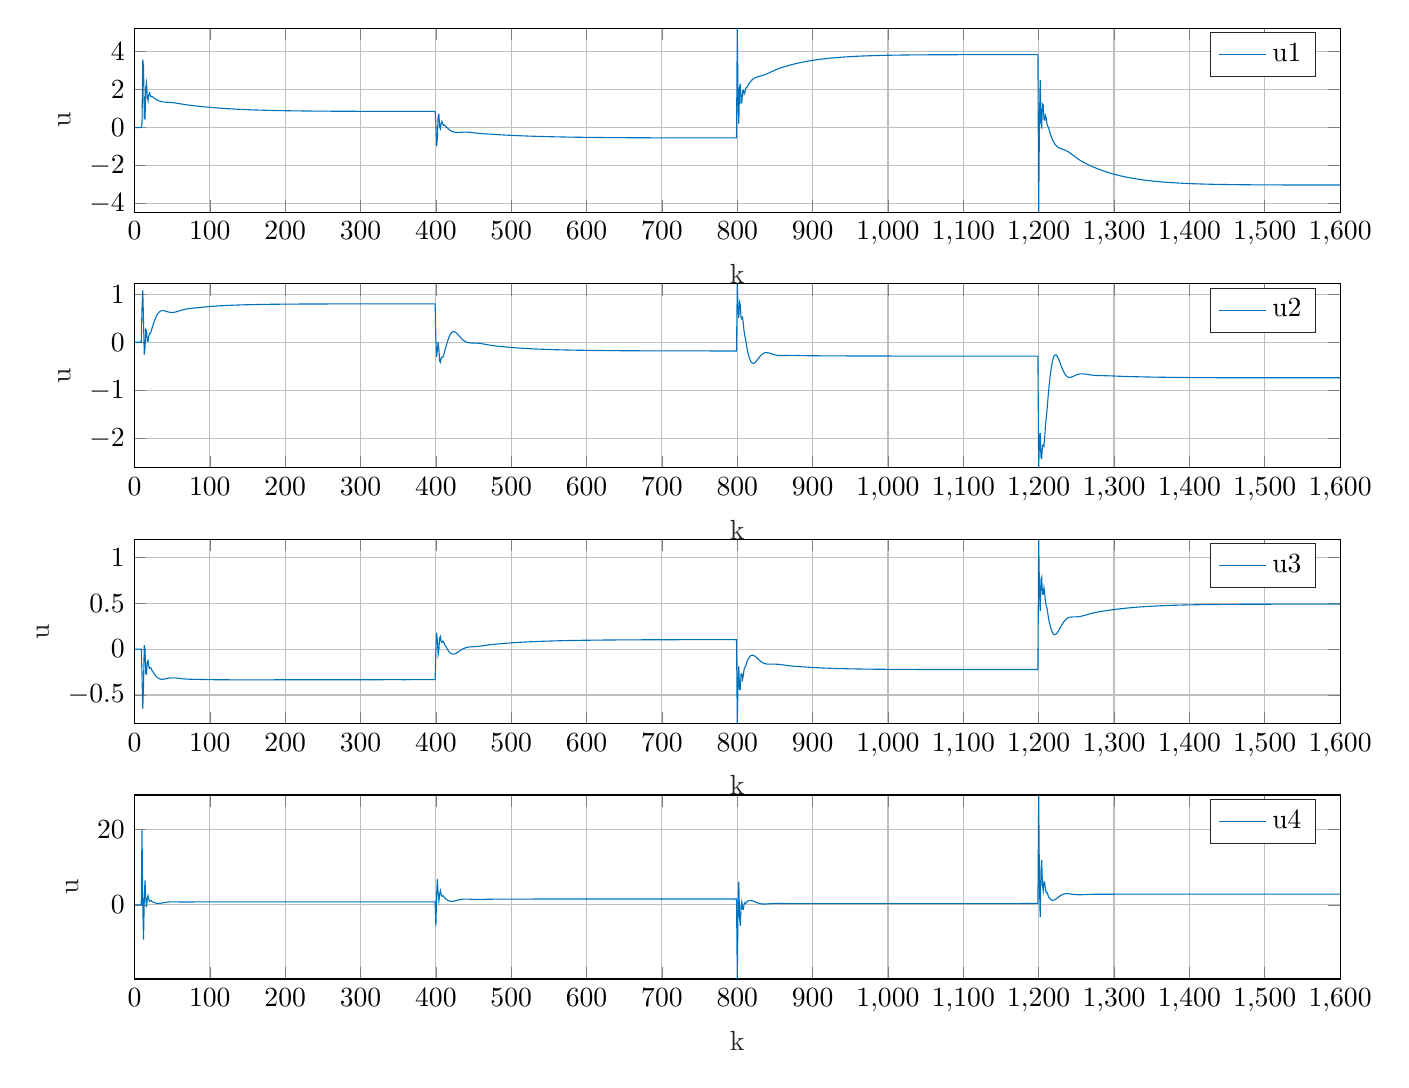
\begin{tikzpicture}

\begin{axis}[%
width=6.028in,
height=0.92in,
at={(1.011in,4.476in)},
scale only axis,
xmin=0,
xmax=1600,
xlabel style={font=\color{white!15!black}},
xlabel={k},
ymin=-4.4552,
ymax=5.23,
ylabel style={font=\color{white!15!black}},
ylabel={u},
axis background/.style={fill=white},
xmajorgrids,
ymajorgrids,
legend style={legend cell align=left, align=left, draw=white!15!black}
]
\addplot [color=mycolor1]
  table[row sep=crcr]{%
1	0\\
2	0\\
3	0\\
4	0\\
5	0\\
6	0\\
7	0\\
8	0\\
9	0\\
10	0.21316\\
11	3.5713\\
12	3.2186\\
13	0.46996\\
14	0.45855\\
15	2.1245\\
16	2.3641\\
17	1.5948\\
18	1.422\\
19	1.7444\\
20	1.8275\\
21	1.6835\\
22	1.6212\\
23	1.642\\
24	1.6274\\
25	1.582\\
26	1.5517\\
27	1.5309\\
28	1.5036\\
29	1.4756\\
30	1.4537\\
31	1.4345\\
32	1.4154\\
33	1.3986\\
34	1.3852\\
35	1.3739\\
36	1.3641\\
37	1.3561\\
38	1.3499\\
39	1.345\\
40	1.341\\
41	1.3378\\
42	1.3353\\
43	1.3331\\
44	1.331\\
45	1.3289\\
46	1.3266\\
47	1.3242\\
48	1.3213\\
49	1.3181\\
50	1.3144\\
51	1.3103\\
52	1.3057\\
53	1.3008\\
54	1.2954\\
55	1.2897\\
56	1.2837\\
57	1.2775\\
58	1.2711\\
59	1.2645\\
60	1.2579\\
61	1.2512\\
62	1.2446\\
63	1.238\\
64	1.2315\\
65	1.2251\\
66	1.2188\\
67	1.2127\\
68	1.2068\\
69	1.201\\
70	1.1953\\
71	1.1898\\
72	1.1845\\
73	1.1793\\
74	1.1743\\
75	1.1693\\
76	1.1645\\
77	1.1598\\
78	1.1552\\
79	1.1506\\
80	1.1461\\
81	1.1417\\
82	1.1373\\
83	1.133\\
84	1.1288\\
85	1.1245\\
86	1.1203\\
87	1.1162\\
88	1.1121\\
89	1.108\\
90	1.1039\\
91	1.1\\
92	1.096\\
93	1.0921\\
94	1.0882\\
95	1.0844\\
96	1.0806\\
97	1.0769\\
98	1.0732\\
99	1.0696\\
100	1.066\\
101	1.0625\\
102	1.059\\
103	1.0556\\
104	1.0522\\
105	1.0489\\
106	1.0457\\
107	1.0425\\
108	1.0393\\
109	1.0362\\
110	1.0332\\
111	1.0302\\
112	1.0272\\
113	1.0243\\
114	1.0214\\
115	1.0186\\
116	1.0158\\
117	1.0131\\
118	1.0104\\
119	1.0077\\
120	1.0051\\
121	1.0026\\
122	1\\
123	0.99752\\
124	0.99507\\
125	0.99264\\
126	0.99026\\
127	0.98791\\
128	0.98559\\
129	0.98332\\
130	0.98107\\
131	0.97886\\
132	0.97669\\
133	0.97455\\
134	0.97244\\
135	0.97037\\
136	0.96833\\
137	0.96632\\
138	0.96434\\
139	0.9624\\
140	0.96048\\
141	0.9586\\
142	0.95675\\
143	0.95492\\
144	0.95313\\
145	0.95136\\
146	0.94963\\
147	0.94792\\
148	0.94624\\
149	0.94459\\
150	0.94296\\
151	0.94136\\
152	0.93979\\
153	0.93824\\
154	0.93672\\
155	0.93522\\
156	0.93374\\
157	0.9323\\
158	0.93087\\
159	0.92947\\
160	0.92809\\
161	0.92673\\
162	0.9254\\
163	0.92408\\
164	0.92279\\
165	0.92152\\
166	0.92027\\
167	0.91905\\
168	0.91784\\
169	0.91665\\
170	0.91548\\
171	0.91434\\
172	0.91321\\
173	0.9121\\
174	0.91101\\
175	0.90993\\
176	0.90888\\
177	0.90784\\
178	0.90682\\
179	0.90582\\
180	0.90483\\
181	0.90386\\
182	0.90291\\
183	0.90197\\
184	0.90105\\
185	0.90015\\
186	0.89926\\
187	0.89839\\
188	0.89753\\
189	0.89668\\
190	0.89585\\
191	0.89504\\
192	0.89424\\
193	0.89345\\
194	0.89268\\
195	0.89192\\
196	0.89117\\
197	0.89043\\
198	0.88971\\
199	0.889\\
200	0.88831\\
201	0.88762\\
202	0.88695\\
203	0.88629\\
204	0.88564\\
205	0.885\\
206	0.88437\\
207	0.88376\\
208	0.88315\\
209	0.88256\\
210	0.88197\\
211	0.8814\\
212	0.88083\\
213	0.88028\\
214	0.87974\\
215	0.8792\\
216	0.87868\\
217	0.87816\\
218	0.87766\\
219	0.87716\\
220	0.87667\\
221	0.87619\\
222	0.87572\\
223	0.87526\\
224	0.8748\\
225	0.87436\\
226	0.87392\\
227	0.87349\\
228	0.87306\\
229	0.87265\\
230	0.87224\\
231	0.87184\\
232	0.87145\\
233	0.87106\\
234	0.87068\\
235	0.87031\\
236	0.86995\\
237	0.86959\\
238	0.86924\\
239	0.86889\\
240	0.86855\\
241	0.86822\\
242	0.86789\\
243	0.86757\\
244	0.86726\\
245	0.86695\\
246	0.86665\\
247	0.86635\\
248	0.86606\\
249	0.86577\\
250	0.86549\\
251	0.86521\\
252	0.86494\\
253	0.86467\\
254	0.86441\\
255	0.86416\\
256	0.86391\\
257	0.86366\\
258	0.86342\\
259	0.86318\\
260	0.86295\\
261	0.86272\\
262	0.86249\\
263	0.86227\\
264	0.86206\\
265	0.86185\\
266	0.86164\\
267	0.86144\\
268	0.86124\\
269	0.86104\\
270	0.86085\\
271	0.86066\\
272	0.86048\\
273	0.86029\\
274	0.86012\\
275	0.85994\\
276	0.85977\\
277	0.8596\\
278	0.85944\\
279	0.85928\\
280	0.85912\\
281	0.85897\\
282	0.85882\\
283	0.85867\\
284	0.85852\\
285	0.85838\\
286	0.85824\\
287	0.8581\\
288	0.85797\\
289	0.85784\\
290	0.85771\\
291	0.85758\\
292	0.85746\\
293	0.85734\\
294	0.85722\\
295	0.8571\\
296	0.85699\\
297	0.85688\\
298	0.85677\\
299	0.85666\\
300	0.85656\\
301	0.85646\\
302	0.85636\\
303	0.85626\\
304	0.85616\\
305	0.85607\\
306	0.85598\\
307	0.85589\\
308	0.8558\\
309	0.85572\\
310	0.85564\\
311	0.85555\\
312	0.85547\\
313	0.8554\\
314	0.85532\\
315	0.85525\\
316	0.85517\\
317	0.8551\\
318	0.85504\\
319	0.85497\\
320	0.8549\\
321	0.85484\\
322	0.85478\\
323	0.85472\\
324	0.85466\\
325	0.8546\\
326	0.85455\\
327	0.85449\\
328	0.85444\\
329	0.85439\\
330	0.85434\\
331	0.85429\\
332	0.85425\\
333	0.8542\\
334	0.85416\\
335	0.85412\\
336	0.85408\\
337	0.85404\\
338	0.854\\
339	0.85396\\
340	0.85393\\
341	0.85389\\
342	0.85386\\
343	0.85383\\
344	0.8538\\
345	0.85377\\
346	0.85374\\
347	0.85371\\
348	0.85369\\
349	0.85366\\
350	0.85363\\
351	0.85361\\
352	0.85358\\
353	0.85356\\
354	0.85353\\
355	0.85351\\
356	0.85348\\
357	0.85346\\
358	0.85343\\
359	0.85341\\
360	0.85339\\
361	0.85319\\
362	0.85318\\
363	0.85327\\
364	0.85322\\
365	0.85313\\
366	0.8531\\
367	0.85309\\
368	0.85305\\
369	0.85302\\
370	0.853\\
371	0.85297\\
372	0.85294\\
373	0.85292\\
374	0.8529\\
375	0.85288\\
376	0.85286\\
377	0.85284\\
378	0.85282\\
379	0.8528\\
380	0.85279\\
381	0.85277\\
382	0.85276\\
383	0.85274\\
384	0.85273\\
385	0.85271\\
386	0.8527\\
387	0.85268\\
388	0.85267\\
389	0.85266\\
390	0.85264\\
391	0.85263\\
392	0.85261\\
393	0.8526\\
394	0.85258\\
395	0.85257\\
396	0.85256\\
397	0.85254\\
398	0.85253\\
399	0.85252\\
400	0.20596\\
401	-0.98237\\
402	-0.57162\\
403	0.64042\\
404	0.68534\\
405	0.033213\\
406	-0.063235\\
407	0.25343\\
408	0.33183\\
409	0.18593\\
410	0.11361\\
411	0.13028\\
412	0.11623\\
413	0.063635\\
414	0.019765\\
415	-0.011893\\
416	-0.047055\\
417	-0.08392\\
418	-0.11568\\
419	-0.14347\\
420	-0.16938\\
421	-0.19198\\
422	-0.21021\\
423	-0.22491\\
424	-0.23673\\
425	-0.24555\\
426	-0.25146\\
427	-0.25501\\
428	-0.25668\\
429	-0.25677\\
430	-0.25561\\
431	-0.25359\\
432	-0.25107\\
433	-0.24831\\
434	-0.24558\\
435	-0.24308\\
436	-0.24099\\
437	-0.23944\\
438	-0.23851\\
439	-0.23827\\
440	-0.23872\\
441	-0.23987\\
442	-0.24169\\
443	-0.24411\\
444	-0.24709\\
445	-0.25055\\
446	-0.25441\\
447	-0.25858\\
448	-0.26299\\
449	-0.26757\\
450	-0.27223\\
451	-0.27692\\
452	-0.28158\\
453	-0.28617\\
454	-0.29064\\
455	-0.29497\\
456	-0.29914\\
457	-0.30312\\
458	-0.30693\\
459	-0.31055\\
460	-0.31399\\
461	-0.31727\\
462	-0.32039\\
463	-0.32337\\
464	-0.32623\\
465	-0.32898\\
466	-0.33164\\
467	-0.33422\\
468	-0.33675\\
469	-0.33923\\
470	-0.34168\\
471	-0.3441\\
472	-0.34651\\
473	-0.34891\\
474	-0.35131\\
475	-0.35371\\
476	-0.35611\\
477	-0.35851\\
478	-0.36091\\
479	-0.36331\\
480	-0.36571\\
481	-0.3681\\
482	-0.37049\\
483	-0.37286\\
484	-0.37521\\
485	-0.37755\\
486	-0.37986\\
487	-0.38215\\
488	-0.38442\\
489	-0.38665\\
490	-0.38886\\
491	-0.39103\\
492	-0.39317\\
493	-0.39529\\
494	-0.39736\\
495	-0.39941\\
496	-0.40143\\
497	-0.40341\\
498	-0.40536\\
499	-0.40729\\
500	-0.40919\\
501	-0.41106\\
502	-0.4129\\
503	-0.41472\\
504	-0.41652\\
505	-0.41829\\
506	-0.42004\\
507	-0.42176\\
508	-0.42347\\
509	-0.42516\\
510	-0.42682\\
511	-0.42847\\
512	-0.43009\\
513	-0.4317\\
514	-0.43329\\
515	-0.43486\\
516	-0.43641\\
517	-0.43794\\
518	-0.43945\\
519	-0.44095\\
520	-0.44242\\
521	-0.44388\\
522	-0.44532\\
523	-0.44674\\
524	-0.44814\\
525	-0.44952\\
526	-0.45089\\
527	-0.45224\\
528	-0.45357\\
529	-0.45488\\
530	-0.45618\\
531	-0.45745\\
532	-0.45872\\
533	-0.45996\\
534	-0.46119\\
535	-0.4624\\
536	-0.4636\\
537	-0.46478\\
538	-0.46594\\
539	-0.46709\\
540	-0.46822\\
541	-0.46934\\
542	-0.47044\\
543	-0.47153\\
544	-0.47261\\
545	-0.47367\\
546	-0.47471\\
547	-0.47575\\
548	-0.47676\\
549	-0.47777\\
550	-0.47876\\
551	-0.47974\\
552	-0.4807\\
553	-0.48165\\
554	-0.48259\\
555	-0.48352\\
556	-0.48443\\
557	-0.48534\\
558	-0.48623\\
559	-0.4871\\
560	-0.48797\\
561	-0.48882\\
562	-0.48966\\
563	-0.4905\\
564	-0.49131\\
565	-0.49212\\
566	-0.49292\\
567	-0.49371\\
568	-0.49448\\
569	-0.49524\\
570	-0.496\\
571	-0.49674\\
572	-0.49747\\
573	-0.4982\\
574	-0.49891\\
575	-0.49961\\
576	-0.50031\\
577	-0.50099\\
578	-0.50166\\
579	-0.50233\\
580	-0.50298\\
581	-0.50363\\
582	-0.50426\\
583	-0.50489\\
584	-0.50551\\
585	-0.50612\\
586	-0.50672\\
587	-0.50731\\
588	-0.5079\\
589	-0.50848\\
590	-0.50904\\
591	-0.5096\\
592	-0.51016\\
593	-0.5107\\
594	-0.51124\\
595	-0.51176\\
596	-0.51229\\
597	-0.5128\\
598	-0.51331\\
599	-0.51381\\
600	-0.5143\\
601	-0.51478\\
602	-0.51526\\
603	-0.51573\\
604	-0.5162\\
605	-0.51665\\
606	-0.5171\\
607	-0.51755\\
608	-0.51799\\
609	-0.51842\\
610	-0.51884\\
611	-0.51926\\
612	-0.51968\\
613	-0.52008\\
614	-0.52048\\
615	-0.52088\\
616	-0.52127\\
617	-0.52165\\
618	-0.52203\\
619	-0.5224\\
620	-0.52277\\
621	-0.52313\\
622	-0.52349\\
623	-0.52384\\
624	-0.52418\\
625	-0.52452\\
626	-0.52486\\
627	-0.52519\\
628	-0.52552\\
629	-0.52584\\
630	-0.52615\\
631	-0.52646\\
632	-0.52677\\
633	-0.52707\\
634	-0.52737\\
635	-0.52766\\
636	-0.52795\\
637	-0.52824\\
638	-0.52852\\
639	-0.52879\\
640	-0.52907\\
641	-0.52933\\
642	-0.5296\\
643	-0.52986\\
644	-0.53011\\
645	-0.53036\\
646	-0.53061\\
647	-0.53086\\
648	-0.5311\\
649	-0.53134\\
650	-0.53157\\
651	-0.5318\\
652	-0.53203\\
653	-0.53225\\
654	-0.53247\\
655	-0.53268\\
656	-0.5329\\
657	-0.53311\\
658	-0.53331\\
659	-0.53352\\
660	-0.53372\\
661	-0.53391\\
662	-0.53411\\
663	-0.5343\\
664	-0.53449\\
665	-0.53467\\
666	-0.53486\\
667	-0.53504\\
668	-0.53521\\
669	-0.53539\\
670	-0.53556\\
671	-0.53573\\
672	-0.53589\\
673	-0.53606\\
674	-0.53622\\
675	-0.53638\\
676	-0.53653\\
677	-0.53669\\
678	-0.53684\\
679	-0.53699\\
680	-0.53714\\
681	-0.53728\\
682	-0.53742\\
683	-0.53756\\
684	-0.5377\\
685	-0.53784\\
686	-0.53797\\
687	-0.5381\\
688	-0.53823\\
689	-0.53836\\
690	-0.53848\\
691	-0.53861\\
692	-0.53873\\
693	-0.53885\\
694	-0.53897\\
695	-0.53908\\
696	-0.5392\\
697	-0.53931\\
698	-0.53942\\
699	-0.53953\\
700	-0.53964\\
701	-0.53974\\
702	-0.53985\\
703	-0.53995\\
704	-0.54005\\
705	-0.54015\\
706	-0.54025\\
707	-0.54035\\
708	-0.54044\\
709	-0.54053\\
710	-0.54063\\
711	-0.54072\\
712	-0.54081\\
713	-0.54089\\
714	-0.54098\\
715	-0.54107\\
716	-0.54115\\
717	-0.54123\\
718	-0.54131\\
719	-0.54139\\
720	-0.54147\\
721	-0.54155\\
722	-0.54163\\
723	-0.5417\\
724	-0.54178\\
725	-0.54185\\
726	-0.54192\\
727	-0.54199\\
728	-0.54206\\
729	-0.54213\\
730	-0.5422\\
731	-0.54227\\
732	-0.54233\\
733	-0.5424\\
734	-0.54246\\
735	-0.54253\\
736	-0.54259\\
737	-0.54265\\
738	-0.54271\\
739	-0.54277\\
740	-0.54283\\
741	-0.54289\\
742	-0.54294\\
743	-0.543\\
744	-0.54305\\
745	-0.54311\\
746	-0.54316\\
747	-0.54321\\
748	-0.54327\\
749	-0.54332\\
750	-0.54337\\
751	-0.54336\\
752	-0.54342\\
753	-0.54353\\
754	-0.54358\\
755	-0.54361\\
756	-0.54366\\
757	-0.54372\\
758	-0.54377\\
759	-0.54381\\
760	-0.54386\\
761	-0.5439\\
762	-0.54394\\
763	-0.54398\\
764	-0.54402\\
765	-0.54406\\
766	-0.54409\\
767	-0.54413\\
768	-0.54416\\
769	-0.54419\\
770	-0.54422\\
771	-0.54425\\
772	-0.54428\\
773	-0.54431\\
774	-0.54434\\
775	-0.54437\\
776	-0.54439\\
777	-0.54442\\
778	-0.54445\\
779	-0.54448\\
780	-0.5445\\
781	-0.54453\\
782	-0.54456\\
783	-0.54458\\
784	-0.54461\\
785	-0.54464\\
786	-0.54467\\
787	-0.54469\\
788	-0.54472\\
789	-0.54474\\
790	-0.54477\\
791	-0.54479\\
792	-0.54482\\
793	-0.54484\\
794	-0.54487\\
795	-0.54489\\
796	-0.54491\\
797	-0.54493\\
798	-0.54496\\
799	-0.54498\\
800	5.23\\
801	1.7352\\
802	0.20672\\
803	2.0563\\
804	2.3147\\
805	1.288\\
806	1.3177\\
807	1.9219\\
808	1.9636\\
809	1.7575\\
810	1.8403\\
811	2.0404\\
812	2.109\\
813	2.1263\\
814	2.1985\\
815	2.286\\
816	2.3433\\
817	2.3884\\
818	2.4388\\
819	2.4855\\
820	2.522\\
821	2.553\\
822	2.5815\\
823	2.6059\\
824	2.6257\\
825	2.6426\\
826	2.6577\\
827	2.6709\\
828	2.6826\\
829	2.6936\\
830	2.7044\\
831	2.7151\\
832	2.7262\\
833	2.7377\\
834	2.75\\
835	2.7631\\
836	2.777\\
837	2.7918\\
838	2.8074\\
839	2.8238\\
840	2.8408\\
841	2.8585\\
842	2.8765\\
843	2.8949\\
844	2.9135\\
845	2.9322\\
846	2.9508\\
847	2.9693\\
848	2.9875\\
849	3.0055\\
850	3.023\\
851	3.0402\\
852	3.0569\\
853	3.0731\\
854	3.0888\\
855	3.1041\\
856	3.1188\\
857	3.1331\\
858	3.147\\
859	3.1604\\
860	3.1735\\
861	3.1862\\
862	3.1986\\
863	3.2106\\
864	3.2224\\
865	3.234\\
866	3.2453\\
867	3.2564\\
868	3.2674\\
869	3.2781\\
870	3.2887\\
871	3.2992\\
872	3.3095\\
873	3.3196\\
874	3.3297\\
875	3.3396\\
876	3.3493\\
877	3.3589\\
878	3.3684\\
879	3.3777\\
880	3.3868\\
881	3.3958\\
882	3.4047\\
883	3.4134\\
884	3.4219\\
885	3.4303\\
886	3.4385\\
887	3.4466\\
888	3.4545\\
889	3.4623\\
890	3.4699\\
891	3.4773\\
892	3.4846\\
893	3.4918\\
894	3.4988\\
895	3.5057\\
896	3.5124\\
897	3.519\\
898	3.5255\\
899	3.5318\\
900	3.538\\
901	3.5441\\
902	3.5501\\
903	3.556\\
904	3.5617\\
905	3.5674\\
906	3.5729\\
907	3.5784\\
908	3.5837\\
909	3.589\\
910	3.5941\\
911	3.5991\\
912	3.6041\\
913	3.6089\\
914	3.6137\\
915	3.6184\\
916	3.623\\
917	3.6275\\
918	3.6319\\
919	3.6362\\
920	3.6404\\
921	3.6446\\
922	3.6487\\
923	3.6527\\
924	3.6566\\
925	3.6604\\
926	3.6642\\
927	3.6679\\
928	3.6715\\
929	3.6751\\
930	3.6786\\
931	3.682\\
932	3.6853\\
933	3.6886\\
934	3.6918\\
935	3.695\\
936	3.698\\
937	3.7011\\
938	3.704\\
939	3.7069\\
940	3.7098\\
941	3.7126\\
942	3.7153\\
943	3.718\\
944	3.7206\\
945	3.7232\\
946	3.7257\\
947	3.7282\\
948	3.7306\\
949	3.733\\
950	3.7353\\
951	3.7376\\
952	3.7398\\
953	3.742\\
954	3.7442\\
955	3.7463\\
956	3.7483\\
957	3.7504\\
958	3.7523\\
959	3.7543\\
960	3.7562\\
961	3.758\\
962	3.7598\\
963	3.7616\\
964	3.7634\\
965	3.7651\\
966	3.7668\\
967	3.7684\\
968	3.77\\
969	3.7716\\
970	3.7731\\
971	3.7746\\
972	3.7761\\
973	3.7775\\
974	3.779\\
975	3.7803\\
976	3.7817\\
977	3.783\\
978	3.7843\\
979	3.7856\\
980	3.7868\\
981	3.7881\\
982	3.7892\\
983	3.7904\\
984	3.7916\\
985	3.7927\\
986	3.7938\\
987	3.7948\\
988	3.7959\\
989	3.7969\\
990	3.7979\\
991	3.7989\\
992	3.7999\\
993	3.8008\\
994	3.8017\\
995	3.8026\\
996	3.8035\\
997	3.8044\\
998	3.8052\\
999	3.806\\
1000	3.8068\\
1001	3.8076\\
1002	3.8084\\
1003	3.8091\\
1004	3.8099\\
1005	3.8106\\
1006	3.8113\\
1007	3.812\\
1008	3.8127\\
1009	3.8133\\
1010	3.814\\
1011	3.8146\\
1012	3.8152\\
1013	3.8158\\
1014	3.8164\\
1015	3.817\\
1016	3.8175\\
1017	3.8181\\
1018	3.8186\\
1019	3.8191\\
1020	3.8196\\
1021	3.8201\\
1022	3.8206\\
1023	3.8211\\
1024	3.8216\\
1025	3.822\\
1026	3.8225\\
1027	3.8229\\
1028	3.8233\\
1029	3.8237\\
1030	3.8241\\
1031	3.8245\\
1032	3.8249\\
1033	3.8253\\
1034	3.8257\\
1035	3.826\\
1036	3.8264\\
1037	3.8267\\
1038	3.827\\
1039	3.8274\\
1040	3.8277\\
1041	3.828\\
1042	3.8283\\
1043	3.8286\\
1044	3.8289\\
1045	3.8292\\
1046	3.8294\\
1047	3.8297\\
1048	3.83\\
1049	3.8302\\
1050	3.8305\\
1051	3.8307\\
1052	3.8309\\
1053	3.8312\\
1054	3.8314\\
1055	3.8316\\
1056	3.8318\\
1057	3.832\\
1058	3.8322\\
1059	3.8324\\
1060	3.8326\\
1061	3.8328\\
1062	3.833\\
1063	3.8331\\
1064	3.8333\\
1065	3.8335\\
1066	3.8336\\
1067	3.8338\\
1068	3.8339\\
1069	3.8341\\
1070	3.8342\\
1071	3.8344\\
1072	3.8345\\
1073	3.8347\\
1074	3.8348\\
1075	3.8349\\
1076	3.835\\
1077	3.8352\\
1078	3.8353\\
1079	3.8354\\
1080	3.8355\\
1081	3.8356\\
1082	3.8357\\
1083	3.8358\\
1084	3.8359\\
1085	3.836\\
1086	3.8361\\
1087	3.8362\\
1088	3.8363\\
1089	3.8363\\
1090	3.8364\\
1091	3.8365\\
1092	3.8366\\
1093	3.8367\\
1094	3.8367\\
1095	3.8368\\
1096	3.8369\\
1097	3.8369\\
1098	3.837\\
1099	3.8371\\
1100	3.8371\\
1101	3.8372\\
1102	3.8372\\
1103	3.8373\\
1104	3.8373\\
1105	3.8374\\
1106	3.8374\\
1107	3.8375\\
1108	3.8375\\
1109	3.8376\\
1110	3.8376\\
1111	3.8376\\
1112	3.8377\\
1113	3.8377\\
1114	3.8378\\
1115	3.8378\\
1116	3.8378\\
1117	3.8379\\
1118	3.8379\\
1119	3.8379\\
1120	3.8379\\
1121	3.838\\
1122	3.838\\
1123	3.838\\
1124	3.8381\\
1125	3.8381\\
1126	3.8381\\
1127	3.8381\\
1128	3.8381\\
1129	3.8382\\
1130	3.8382\\
1131	3.8382\\
1132	3.8382\\
1133	3.8382\\
1134	3.8383\\
1135	3.8383\\
1136	3.8383\\
1137	3.8383\\
1138	3.8383\\
1139	3.8383\\
1140	3.8383\\
1141	3.8384\\
1142	3.8384\\
1143	3.8384\\
1144	3.8384\\
1145	3.8384\\
1146	3.8384\\
1147	3.8384\\
1148	3.8385\\
1149	3.8385\\
1150	3.8385\\
1151	3.8386\\
1152	3.8386\\
1153	3.8385\\
1154	3.8386\\
1155	3.8386\\
1156	3.8386\\
1157	3.8386\\
1158	3.8387\\
1159	3.8387\\
1160	3.8387\\
1161	3.8387\\
1162	3.8387\\
1163	3.8387\\
1164	3.8387\\
1165	3.8386\\
1166	3.8386\\
1167	3.8386\\
1168	3.8386\\
1169	3.8386\\
1170	3.8386\\
1171	3.8386\\
1172	3.8386\\
1173	3.8386\\
1174	3.8386\\
1175	3.8386\\
1176	3.8386\\
1177	3.8386\\
1178	3.8386\\
1179	3.8385\\
1180	3.8385\\
1181	3.8385\\
1182	3.8385\\
1183	3.8385\\
1184	3.8385\\
1185	3.8385\\
1186	3.8385\\
1187	3.8385\\
1188	3.8385\\
1189	3.8385\\
1190	3.8385\\
1191	3.8385\\
1192	3.8385\\
1193	3.8385\\
1194	3.8385\\
1195	3.8385\\
1196	3.8385\\
1197	3.8385\\
1198	3.8385\\
1199	3.8385\\
1200	-4.4552\\
1201	0.19455\\
1202	2.5081\\
1203	0.26844\\
1204	-0.04733\\
1205	1.2506\\
1206	1.1951\\
1207	0.43249\\
1208	0.39436\\
1209	0.63922\\
1210	0.4897\\
1211	0.19392\\
1212	0.072756\\
1213	0.011476\\
1214	-0.12656\\
1215	-0.28332\\
1216	-0.39808\\
1217	-0.49519\\
1218	-0.59706\\
1219	-0.6908\\
1220	-0.76744\\
1221	-0.83329\\
1222	-0.89212\\
1223	-0.94174\\
1224	-0.98194\\
1225	-1.0153\\
1226	-1.0432\\
1227	-1.0661\\
1228	-1.0851\\
1229	-1.1014\\
1230	-1.1161\\
1231	-1.1298\\
1232	-1.1434\\
1233	-1.1573\\
1234	-1.1723\\
1235	-1.1885\\
1236	-1.2062\\
1237	-1.2257\\
1238	-1.2468\\
1239	-1.2697\\
1240	-1.2941\\
1241	-1.3201\\
1242	-1.3473\\
1243	-1.3755\\
1244	-1.4046\\
1245	-1.4343\\
1246	-1.4643\\
1247	-1.4944\\
1248	-1.5245\\
1249	-1.5543\\
1250	-1.5838\\
1251	-1.6127\\
1252	-1.6409\\
1253	-1.6684\\
1254	-1.6952\\
1255	-1.7211\\
1256	-1.7462\\
1257	-1.7706\\
1258	-1.7941\\
1259	-1.8168\\
1260	-1.8389\\
1261	-1.8603\\
1262	-1.881\\
1263	-1.9012\\
1264	-1.9209\\
1265	-1.9402\\
1266	-1.959\\
1267	-1.9775\\
1268	-1.9956\\
1269	-2.0135\\
1270	-2.0311\\
1271	-2.0484\\
1272	-2.0656\\
1273	-2.0825\\
1274	-2.0992\\
1275	-2.1157\\
1276	-2.132\\
1277	-2.1481\\
1278	-2.164\\
1279	-2.1797\\
1280	-2.1952\\
1281	-2.2104\\
1282	-2.2255\\
1283	-2.2403\\
1284	-2.2548\\
1285	-2.2691\\
1286	-2.2832\\
1287	-2.297\\
1288	-2.3106\\
1289	-2.3239\\
1290	-2.337\\
1291	-2.3499\\
1292	-2.3624\\
1293	-2.3748\\
1294	-2.3869\\
1295	-2.3988\\
1296	-2.4105\\
1297	-2.4219\\
1298	-2.4331\\
1299	-2.4442\\
1300	-2.455\\
1301	-2.4656\\
1302	-2.476\\
1303	-2.4863\\
1304	-2.4963\\
1305	-2.5062\\
1306	-2.5159\\
1307	-2.5254\\
1308	-2.5348\\
1309	-2.544\\
1310	-2.5531\\
1311	-2.5619\\
1312	-2.5707\\
1313	-2.5793\\
1314	-2.5877\\
1315	-2.596\\
1316	-2.6041\\
1317	-2.6121\\
1318	-2.6199\\
1319	-2.6276\\
1320	-2.6352\\
1321	-2.6426\\
1322	-2.6499\\
1323	-2.6571\\
1324	-2.6642\\
1325	-2.6711\\
1326	-2.6779\\
1327	-2.6845\\
1328	-2.691\\
1329	-2.6975\\
1330	-2.7038\\
1331	-2.71\\
1332	-2.716\\
1333	-2.722\\
1334	-2.7278\\
1335	-2.7336\\
1336	-2.7392\\
1337	-2.7448\\
1338	-2.7502\\
1339	-2.7555\\
1340	-2.7608\\
1341	-2.7659\\
1342	-2.7709\\
1343	-2.7759\\
1344	-2.7807\\
1345	-2.7855\\
1346	-2.7902\\
1347	-2.7948\\
1348	-2.7993\\
1349	-2.8037\\
1350	-2.8081\\
1351	-2.8123\\
1352	-2.8165\\
1353	-2.8206\\
1354	-2.8247\\
1355	-2.8286\\
1356	-2.8325\\
1357	-2.8363\\
1358	-2.8401\\
1359	-2.8437\\
1360	-2.8473\\
1361	-2.8509\\
1362	-2.8543\\
1363	-2.8577\\
1364	-2.8611\\
1365	-2.8643\\
1366	-2.8675\\
1367	-2.8707\\
1368	-2.8738\\
1369	-2.8768\\
1370	-2.8798\\
1371	-2.8827\\
1372	-2.8856\\
1373	-2.8884\\
1374	-2.8911\\
1375	-2.8938\\
1376	-2.8965\\
1377	-2.8991\\
1378	-2.9016\\
1379	-2.9041\\
1380	-2.9066\\
1381	-2.909\\
1382	-2.9113\\
1383	-2.9137\\
1384	-2.9159\\
1385	-2.9182\\
1386	-2.9203\\
1387	-2.9225\\
1388	-2.9246\\
1389	-2.9266\\
1390	-2.9286\\
1391	-2.9306\\
1392	-2.9326\\
1393	-2.9345\\
1394	-2.9363\\
1395	-2.9382\\
1396	-2.9399\\
1397	-2.9417\\
1398	-2.9434\\
1399	-2.9451\\
1400	-2.9468\\
1401	-2.9484\\
1402	-2.95\\
1403	-2.9515\\
1404	-2.9531\\
1405	-2.9546\\
1406	-2.956\\
1407	-2.9575\\
1408	-2.9589\\
1409	-2.9603\\
1410	-2.9616\\
1411	-2.963\\
1412	-2.9643\\
1413	-2.9655\\
1414	-2.9668\\
1415	-2.968\\
1416	-2.9692\\
1417	-2.9704\\
1418	-2.9715\\
1419	-2.9727\\
1420	-2.9738\\
1421	-2.9749\\
1422	-2.9759\\
1423	-2.977\\
1424	-2.978\\
1425	-2.979\\
1426	-2.9799\\
1427	-2.9809\\
1428	-2.9818\\
1429	-2.9828\\
1430	-2.9837\\
1431	-2.9845\\
1432	-2.9854\\
1433	-2.9863\\
1434	-2.9871\\
1435	-2.9879\\
1436	-2.9887\\
1437	-2.9895\\
1438	-2.9902\\
1439	-2.991\\
1440	-2.9917\\
1441	-2.9924\\
1442	-2.9931\\
1443	-2.9938\\
1444	-2.9945\\
1445	-2.9951\\
1446	-2.9958\\
1447	-2.9964\\
1448	-2.997\\
1449	-2.9976\\
1450	-2.9982\\
1451	-2.9988\\
1452	-2.9994\\
1453	-2.9999\\
1454	-3.0004\\
1455	-3.001\\
1456	-3.0015\\
1457	-3.002\\
1458	-3.0025\\
1459	-3.003\\
1460	-3.0035\\
1461	-3.0039\\
1462	-3.0044\\
1463	-3.0048\\
1464	-3.0053\\
1465	-3.0057\\
1466	-3.0061\\
1467	-3.0065\\
1468	-3.0069\\
1469	-3.0073\\
1470	-3.0077\\
1471	-3.0081\\
1472	-3.0084\\
1473	-3.0088\\
1474	-3.0091\\
1475	-3.0095\\
1476	-3.0098\\
1477	-3.0101\\
1478	-3.0104\\
1479	-3.0108\\
1480	-3.0111\\
1481	-3.0114\\
1482	-3.0117\\
1483	-3.0119\\
1484	-3.0122\\
1485	-3.0125\\
1486	-3.0128\\
1487	-3.013\\
1488	-3.0133\\
1489	-3.0135\\
1490	-3.0138\\
1491	-3.014\\
1492	-3.0142\\
1493	-3.0145\\
1494	-3.0147\\
1495	-3.0149\\
1496	-3.0151\\
1497	-3.0153\\
1498	-3.0155\\
1499	-3.0157\\
1500	-3.0159\\
1501	-3.0161\\
1502	-3.0163\\
1503	-3.0164\\
1504	-3.0166\\
1505	-3.0168\\
1506	-3.017\\
1507	-3.0171\\
1508	-3.0173\\
1509	-3.0174\\
1510	-3.0176\\
1511	-3.0177\\
1512	-3.0179\\
1513	-3.018\\
1514	-3.0181\\
1515	-3.0183\\
1516	-3.0184\\
1517	-3.0185\\
1518	-3.0187\\
1519	-3.0188\\
1520	-3.0189\\
1521	-3.019\\
1522	-3.0191\\
1523	-3.0192\\
1524	-3.0193\\
1525	-3.0194\\
1526	-3.0195\\
1527	-3.0196\\
1528	-3.0197\\
1529	-3.0198\\
1530	-3.0199\\
1531	-3.02\\
1532	-3.0201\\
1533	-3.0202\\
1534	-3.0203\\
1535	-3.0204\\
1536	-3.0204\\
1537	-3.0205\\
1538	-3.0206\\
1539	-3.0207\\
1540	-3.0207\\
1541	-3.0208\\
1542	-3.0209\\
1543	-3.021\\
1544	-3.021\\
1545	-3.0211\\
1546	-3.0212\\
1547	-3.0213\\
1548	-3.0213\\
1549	-3.0214\\
1550	-3.0215\\
1551	-3.0217\\
1552	-3.0217\\
1553	-3.0217\\
1554	-3.0218\\
1555	-3.0219\\
1556	-3.022\\
1557	-3.022\\
1558	-3.0221\\
1559	-3.0222\\
1560	-3.0222\\
1561	-3.0222\\
1562	-3.0223\\
1563	-3.0223\\
1564	-3.0224\\
1565	-3.0224\\
1566	-3.0224\\
1567	-3.0224\\
1568	-3.0224\\
1569	-3.0225\\
1570	-3.0225\\
1571	-3.0225\\
1572	-3.0225\\
1573	-3.0225\\
1574	-3.0226\\
1575	-3.0226\\
1576	-3.0226\\
1577	-3.0226\\
1578	-3.0226\\
1579	-3.0227\\
1580	-3.0227\\
1581	-3.0227\\
1582	-3.0227\\
1583	-3.0227\\
1584	-3.0228\\
1585	-3.0228\\
1586	-3.0228\\
1587	-3.0228\\
1588	-3.0229\\
1589	-3.0229\\
1590	-3.0229\\
1591	-3.0229\\
1592	-3.0229\\
1593	-3.0229\\
1594	-3.023\\
1595	-3.023\\
1596	-3.023\\
1597	-3.023\\
1598	-3.023\\
1599	-3.023\\
1600	-3.023\\
};
\addlegendentry{u1}

\end{axis}

\begin{axis}[%
width=6.028in,
height=0.92in,
at={(1.011in,3.198in)},
scale only axis,
xmin=0,
xmax=1600,
xlabel style={font=\color{white!15!black}},
xlabel={k},
ymin=-2.612,
ymax=1.2152,
ylabel style={font=\color{white!15!black}},
ylabel={u},
axis background/.style={fill=white},
xmajorgrids,
ymajorgrids,
legend style={legend cell align=left, align=left, draw=white!15!black}
]
\addplot [color=mycolor1]
  table[row sep=crcr]{%
1	0\\
2	0\\
3	0\\
4	0\\
5	0\\
6	0\\
7	0\\
8	0\\
9	0\\
10	0.70951\\
11	1.0794\\
12	0.44827\\
13	-0.256\\
14	-0.12248\\
15	0.26457\\
16	0.23466\\
17	0.026807\\
18	0.016006\\
19	0.12676\\
20	0.17853\\
21	0.1856\\
22	0.22025\\
23	0.27797\\
24	0.32917\\
25	0.37336\\
26	0.41879\\
27	0.4631\\
28	0.50226\\
29	0.53692\\
30	0.56779\\
31	0.59386\\
32	0.61473\\
33	0.63109\\
34	0.64343\\
35	0.65187\\
36	0.6568\\
37	0.65885\\
38	0.65857\\
39	0.65643\\
40	0.65292\\
41	0.64851\\
42	0.64365\\
43	0.63867\\
44	0.63391\\
45	0.62961\\
46	0.62598\\
47	0.62314\\
48	0.62119\\
49	0.62018\\
50	0.6201\\
51	0.62093\\
52	0.6226\\
53	0.62502\\
54	0.62812\\
55	0.63177\\
56	0.63587\\
57	0.64031\\
58	0.64497\\
59	0.64977\\
60	0.65461\\
61	0.65941\\
62	0.66411\\
63	0.66864\\
64	0.67297\\
65	0.67707\\
66	0.68091\\
67	0.68449\\
68	0.6878\\
69	0.69086\\
70	0.69368\\
71	0.69627\\
72	0.69865\\
73	0.70085\\
74	0.7029\\
75	0.70481\\
76	0.70661\\
77	0.70832\\
78	0.70997\\
79	0.71157\\
80	0.71313\\
81	0.71467\\
82	0.7162\\
83	0.71773\\
84	0.71926\\
85	0.72079\\
86	0.72233\\
87	0.72388\\
88	0.72543\\
89	0.72699\\
90	0.72854\\
91	0.73008\\
92	0.73162\\
93	0.73314\\
94	0.73465\\
95	0.73613\\
96	0.73759\\
97	0.73901\\
98	0.74041\\
99	0.74177\\
100	0.7431\\
101	0.7444\\
102	0.74565\\
103	0.74687\\
104	0.74806\\
105	0.74921\\
106	0.75033\\
107	0.75141\\
108	0.75247\\
109	0.75349\\
110	0.75449\\
111	0.75546\\
112	0.75641\\
113	0.75733\\
114	0.75823\\
115	0.75911\\
116	0.75997\\
117	0.76081\\
118	0.76163\\
119	0.76244\\
120	0.76323\\
121	0.764\\
122	0.76476\\
123	0.7655\\
124	0.76623\\
125	0.76695\\
126	0.76765\\
127	0.76833\\
128	0.769\\
129	0.76966\\
130	0.7703\\
131	0.77093\\
132	0.77154\\
133	0.77215\\
134	0.77273\\
135	0.77331\\
136	0.77387\\
137	0.77442\\
138	0.77496\\
139	0.77548\\
140	0.77599\\
141	0.77649\\
142	0.77698\\
143	0.77746\\
144	0.77793\\
145	0.77838\\
146	0.77883\\
147	0.77926\\
148	0.77969\\
149	0.78011\\
150	0.78051\\
151	0.78091\\
152	0.7813\\
153	0.78168\\
154	0.78205\\
155	0.78241\\
156	0.78277\\
157	0.78311\\
158	0.78345\\
159	0.78379\\
160	0.78411\\
161	0.78443\\
162	0.78474\\
163	0.78504\\
164	0.78534\\
165	0.78563\\
166	0.78591\\
167	0.78619\\
168	0.78646\\
169	0.78673\\
170	0.78699\\
171	0.78724\\
172	0.78749\\
173	0.78773\\
174	0.78797\\
175	0.7882\\
176	0.78843\\
177	0.78865\\
178	0.78886\\
179	0.78908\\
180	0.78928\\
181	0.78948\\
182	0.78968\\
183	0.78988\\
184	0.79007\\
185	0.79025\\
186	0.79043\\
187	0.79061\\
188	0.79078\\
189	0.79095\\
190	0.79111\\
191	0.79128\\
192	0.79143\\
193	0.79159\\
194	0.79174\\
195	0.79189\\
196	0.79203\\
197	0.79217\\
198	0.79231\\
199	0.79245\\
200	0.79258\\
201	0.79271\\
202	0.79283\\
203	0.79296\\
204	0.79308\\
205	0.7932\\
206	0.79331\\
207	0.79342\\
208	0.79353\\
209	0.79364\\
210	0.79375\\
211	0.79385\\
212	0.79395\\
213	0.79405\\
214	0.79415\\
215	0.79424\\
216	0.79433\\
217	0.79443\\
218	0.79451\\
219	0.7946\\
220	0.79469\\
221	0.79477\\
222	0.79485\\
223	0.79493\\
224	0.79501\\
225	0.79508\\
226	0.79516\\
227	0.79523\\
228	0.7953\\
229	0.79537\\
230	0.79544\\
231	0.7955\\
232	0.79557\\
233	0.79563\\
234	0.79569\\
235	0.79575\\
236	0.79581\\
237	0.79587\\
238	0.79593\\
239	0.79598\\
240	0.79604\\
241	0.79609\\
242	0.79614\\
243	0.7962\\
244	0.79625\\
245	0.79629\\
246	0.79634\\
247	0.79639\\
248	0.79643\\
249	0.79648\\
250	0.79652\\
251	0.79657\\
252	0.79661\\
253	0.79665\\
254	0.79669\\
255	0.79673\\
256	0.79677\\
257	0.79681\\
258	0.79684\\
259	0.79688\\
260	0.79691\\
261	0.79695\\
262	0.79698\\
263	0.79702\\
264	0.79705\\
265	0.79708\\
266	0.79711\\
267	0.79714\\
268	0.79717\\
269	0.7972\\
270	0.79723\\
271	0.79726\\
272	0.79728\\
273	0.79731\\
274	0.79734\\
275	0.79736\\
276	0.79739\\
277	0.79741\\
278	0.79744\\
279	0.79746\\
280	0.79748\\
281	0.79751\\
282	0.79753\\
283	0.79755\\
284	0.79757\\
285	0.79759\\
286	0.79761\\
287	0.79763\\
288	0.79765\\
289	0.79767\\
290	0.79769\\
291	0.79771\\
292	0.79773\\
293	0.79774\\
294	0.79776\\
295	0.79778\\
296	0.79779\\
297	0.79781\\
298	0.79783\\
299	0.79784\\
300	0.79786\\
301	0.79787\\
302	0.79789\\
303	0.7979\\
304	0.79791\\
305	0.79793\\
306	0.79794\\
307	0.79796\\
308	0.79797\\
309	0.79798\\
310	0.79799\\
311	0.79801\\
312	0.79802\\
313	0.79803\\
314	0.79804\\
315	0.79805\\
316	0.79807\\
317	0.79808\\
318	0.79809\\
319	0.7981\\
320	0.79811\\
321	0.79812\\
322	0.79813\\
323	0.79814\\
324	0.79815\\
325	0.79816\\
326	0.79817\\
327	0.79818\\
328	0.79819\\
329	0.7982\\
330	0.79821\\
331	0.79822\\
332	0.79823\\
333	0.79823\\
334	0.79824\\
335	0.79825\\
336	0.79826\\
337	0.79827\\
338	0.79828\\
339	0.79829\\
340	0.7983\\
341	0.7983\\
342	0.79831\\
343	0.79832\\
344	0.79833\\
345	0.79834\\
346	0.79834\\
347	0.79835\\
348	0.79836\\
349	0.79837\\
350	0.79838\\
351	0.79838\\
352	0.79839\\
353	0.7984\\
354	0.79841\\
355	0.79841\\
356	0.79842\\
357	0.79843\\
358	0.79844\\
359	0.79844\\
360	0.79845\\
361	0.79842\\
362	0.79844\\
363	0.79849\\
364	0.7985\\
365	0.79849\\
366	0.7985\\
367	0.79851\\
368	0.79852\\
369	0.79852\\
370	0.79853\\
371	0.79854\\
372	0.79854\\
373	0.79855\\
374	0.79855\\
375	0.79856\\
376	0.79856\\
377	0.79856\\
378	0.79856\\
379	0.79856\\
380	0.79857\\
381	0.79857\\
382	0.79857\\
383	0.79857\\
384	0.79857\\
385	0.79857\\
386	0.79857\\
387	0.79858\\
388	0.79858\\
389	0.79858\\
390	0.79858\\
391	0.79859\\
392	0.79859\\
393	0.79859\\
394	0.7986\\
395	0.7986\\
396	0.79861\\
397	0.79861\\
398	0.79861\\
399	0.79862\\
400	0.045444\\
401	-0.30434\\
402	-0.15879\\
403	0.0078327\\
404	-0.15491\\
405	-0.38821\\
406	-0.4154\\
407	-0.33476\\
408	-0.30827\\
409	-0.31608\\
410	-0.28727\\
411	-0.22705\\
412	-0.16874\\
413	-0.1166\\
414	-0.062235\\
415	-0.0071405\\
416	0.043365\\
417	0.088086\\
418	0.12722\\
419	0.15981\\
420	0.18522\\
421	0.20376\\
422	0.21584\\
423	0.22173\\
424	0.22192\\
425	0.21724\\
426	0.20846\\
427	0.19633\\
428	0.1816\\
429	0.16506\\
430	0.14741\\
431	0.12927\\
432	0.11119\\
433	0.093642\\
434	0.077004\\
435	0.061565\\
436	0.047533\\
437	0.035036\\
438	0.024135\\
439	0.014825\\
440	0.0070533\\
441	0.00072328\\
442	-0.0042927\\
443	-0.0081453\\
444	-0.010999\\
445	-0.013025\\
446	-0.014392\\
447	-0.015266\\
448	-0.015798\\
449	-0.016128\\
450	-0.016377\\
451	-0.01665\\
452	-0.01703\\
453	-0.017583\\
454	-0.018358\\
455	-0.019385\\
456	-0.02068\\
457	-0.022245\\
458	-0.024072\\
459	-0.026143\\
460	-0.028433\\
461	-0.030911\\
462	-0.033545\\
463	-0.036299\\
464	-0.039139\\
465	-0.042031\\
466	-0.044943\\
467	-0.047847\\
468	-0.050718\\
469	-0.053534\\
470	-0.056279\\
471	-0.058938\\
472	-0.061503\\
473	-0.063967\\
474	-0.066327\\
475	-0.068584\\
476	-0.07074\\
477	-0.0728\\
478	-0.074769\\
479	-0.076655\\
480	-0.078465\\
481	-0.080208\\
482	-0.081891\\
483	-0.083523\\
484	-0.085111\\
485	-0.086662\\
486	-0.088182\\
487	-0.089676\\
488	-0.091148\\
489	-0.092602\\
490	-0.094042\\
491	-0.095468\\
492	-0.096882\\
493	-0.098285\\
494	-0.099676\\
495	-0.10106\\
496	-0.10242\\
497	-0.10378\\
498	-0.10512\\
499	-0.10644\\
500	-0.10775\\
501	-0.10904\\
502	-0.11031\\
503	-0.11157\\
504	-0.1128\\
505	-0.11401\\
506	-0.1152\\
507	-0.11636\\
508	-0.11751\\
509	-0.11863\\
510	-0.11973\\
511	-0.12081\\
512	-0.12186\\
513	-0.1229\\
514	-0.12391\\
515	-0.12491\\
516	-0.12588\\
517	-0.12684\\
518	-0.12778\\
519	-0.12871\\
520	-0.12961\\
521	-0.1305\\
522	-0.13138\\
523	-0.13224\\
524	-0.13308\\
525	-0.13391\\
526	-0.13473\\
527	-0.13553\\
528	-0.13632\\
529	-0.1371\\
530	-0.13786\\
531	-0.13861\\
532	-0.13935\\
533	-0.14008\\
534	-0.14079\\
535	-0.1415\\
536	-0.14219\\
537	-0.14287\\
538	-0.14353\\
539	-0.14419\\
540	-0.14484\\
541	-0.14547\\
542	-0.14609\\
543	-0.14671\\
544	-0.14731\\
545	-0.1479\\
546	-0.14848\\
547	-0.14905\\
548	-0.14961\\
549	-0.15016\\
550	-0.15071\\
551	-0.15124\\
552	-0.15176\\
553	-0.15227\\
554	-0.15278\\
555	-0.15328\\
556	-0.15376\\
557	-0.15424\\
558	-0.15471\\
559	-0.15518\\
560	-0.15563\\
561	-0.15608\\
562	-0.15652\\
563	-0.15695\\
564	-0.15738\\
565	-0.15779\\
566	-0.1582\\
567	-0.15861\\
568	-0.159\\
569	-0.15939\\
570	-0.15977\\
571	-0.16015\\
572	-0.16052\\
573	-0.16088\\
574	-0.16124\\
575	-0.16159\\
576	-0.16194\\
577	-0.16227\\
578	-0.16261\\
579	-0.16294\\
580	-0.16326\\
581	-0.16357\\
582	-0.16388\\
583	-0.16419\\
584	-0.16449\\
585	-0.16479\\
586	-0.16508\\
587	-0.16536\\
588	-0.16564\\
589	-0.16592\\
590	-0.16619\\
591	-0.16645\\
592	-0.16671\\
593	-0.16697\\
594	-0.16722\\
595	-0.16747\\
596	-0.16772\\
597	-0.16795\\
598	-0.16819\\
599	-0.16842\\
600	-0.16865\\
601	-0.16887\\
602	-0.16909\\
603	-0.16931\\
604	-0.16952\\
605	-0.16973\\
606	-0.16993\\
607	-0.17013\\
608	-0.17033\\
609	-0.17053\\
610	-0.17072\\
611	-0.17091\\
612	-0.17109\\
613	-0.17127\\
614	-0.17145\\
615	-0.17163\\
616	-0.1718\\
617	-0.17197\\
618	-0.17213\\
619	-0.1723\\
620	-0.17246\\
621	-0.17262\\
622	-0.17277\\
623	-0.17292\\
624	-0.17307\\
625	-0.17322\\
626	-0.17337\\
627	-0.17351\\
628	-0.17365\\
629	-0.17379\\
630	-0.17392\\
631	-0.17405\\
632	-0.17418\\
633	-0.17431\\
634	-0.17444\\
635	-0.17456\\
636	-0.17468\\
637	-0.1748\\
638	-0.17492\\
639	-0.17504\\
640	-0.17515\\
641	-0.17526\\
642	-0.17537\\
643	-0.17548\\
644	-0.17558\\
645	-0.17569\\
646	-0.17579\\
647	-0.17589\\
648	-0.17599\\
649	-0.17609\\
650	-0.17618\\
651	-0.17627\\
652	-0.17637\\
653	-0.17646\\
654	-0.17655\\
655	-0.17663\\
656	-0.17672\\
657	-0.1768\\
658	-0.17689\\
659	-0.17697\\
660	-0.17705\\
661	-0.17713\\
662	-0.1772\\
663	-0.17728\\
664	-0.17736\\
665	-0.17743\\
666	-0.1775\\
667	-0.17757\\
668	-0.17764\\
669	-0.17771\\
670	-0.17778\\
671	-0.17784\\
672	-0.17791\\
673	-0.17797\\
674	-0.17803\\
675	-0.1781\\
676	-0.17816\\
677	-0.17822\\
678	-0.17828\\
679	-0.17833\\
680	-0.17839\\
681	-0.17845\\
682	-0.1785\\
683	-0.17855\\
684	-0.17861\\
685	-0.17866\\
686	-0.17871\\
687	-0.17876\\
688	-0.17881\\
689	-0.17886\\
690	-0.1789\\
691	-0.17895\\
692	-0.179\\
693	-0.17904\\
694	-0.17909\\
695	-0.17913\\
696	-0.17917\\
697	-0.17922\\
698	-0.17926\\
699	-0.1793\\
700	-0.17934\\
701	-0.17938\\
702	-0.17942\\
703	-0.17945\\
704	-0.17949\\
705	-0.17953\\
706	-0.17956\\
707	-0.1796\\
708	-0.17964\\
709	-0.17967\\
710	-0.1797\\
711	-0.17974\\
712	-0.17977\\
713	-0.1798\\
714	-0.17983\\
715	-0.17986\\
716	-0.17989\\
717	-0.17992\\
718	-0.17995\\
719	-0.17998\\
720	-0.18001\\
721	-0.18004\\
722	-0.18007\\
723	-0.18009\\
724	-0.18012\\
725	-0.18014\\
726	-0.18017\\
727	-0.1802\\
728	-0.18022\\
729	-0.18024\\
730	-0.18027\\
731	-0.18029\\
732	-0.18031\\
733	-0.18034\\
734	-0.18036\\
735	-0.18038\\
736	-0.1804\\
737	-0.18042\\
738	-0.18044\\
739	-0.18047\\
740	-0.18049\\
741	-0.1805\\
742	-0.18052\\
743	-0.18054\\
744	-0.18056\\
745	-0.18058\\
746	-0.1806\\
747	-0.18062\\
748	-0.18063\\
749	-0.18065\\
750	-0.18067\\
751	-0.18067\\
752	-0.18069\\
753	-0.18072\\
754	-0.18074\\
755	-0.18074\\
756	-0.18076\\
757	-0.18077\\
758	-0.18078\\
759	-0.18079\\
760	-0.1808\\
761	-0.18081\\
762	-0.18082\\
763	-0.18083\\
764	-0.18084\\
765	-0.18085\\
766	-0.18086\\
767	-0.18087\\
768	-0.18089\\
769	-0.1809\\
770	-0.18092\\
771	-0.18093\\
772	-0.18094\\
773	-0.18096\\
774	-0.18097\\
775	-0.18099\\
776	-0.181\\
777	-0.18101\\
778	-0.18103\\
779	-0.18104\\
780	-0.18105\\
781	-0.18106\\
782	-0.18107\\
783	-0.18108\\
784	-0.18109\\
785	-0.1811\\
786	-0.1811\\
787	-0.18111\\
788	-0.18112\\
789	-0.18112\\
790	-0.18113\\
791	-0.18114\\
792	-0.18114\\
793	-0.18115\\
794	-0.18116\\
795	-0.18116\\
796	-0.18117\\
797	-0.18118\\
798	-0.18118\\
799	-0.18119\\
800	1.2152\\
801	0.69358\\
802	0.50045\\
803	0.83518\\
804	0.78013\\
805	0.51758\\
806	0.4861\\
807	0.5158\\
808	0.3938\\
809	0.2303\\
810	0.1377\\
811	0.066576\\
812	-0.031518\\
813	-0.13028\\
814	-0.20541\\
815	-0.26641\\
816	-0.32206\\
817	-0.36759\\
818	-0.39973\\
819	-0.42128\\
820	-0.43441\\
821	-0.43913\\
822	-0.43621\\
823	-0.4274\\
824	-0.41409\\
825	-0.39725\\
826	-0.37798\\
827	-0.35745\\
828	-0.33659\\
829	-0.31615\\
830	-0.29678\\
831	-0.27901\\
832	-0.26323\\
833	-0.24967\\
834	-0.23847\\
835	-0.22967\\
836	-0.22321\\
837	-0.21897\\
838	-0.21677\\
839	-0.21637\\
840	-0.21754\\
841	-0.22\\
842	-0.22349\\
843	-0.22775\\
844	-0.23253\\
845	-0.2376\\
846	-0.24277\\
847	-0.24785\\
848	-0.25272\\
849	-0.25725\\
850	-0.26136\\
851	-0.26499\\
852	-0.26812\\
853	-0.27072\\
854	-0.27282\\
855	-0.27443\\
856	-0.2756\\
857	-0.27637\\
858	-0.27678\\
859	-0.27691\\
860	-0.2768\\
861	-0.2765\\
862	-0.27608\\
863	-0.27558\\
864	-0.27505\\
865	-0.27451\\
866	-0.27401\\
867	-0.27356\\
868	-0.27319\\
869	-0.2729\\
870	-0.27271\\
871	-0.27262\\
872	-0.27262\\
873	-0.27271\\
874	-0.27289\\
875	-0.27315\\
876	-0.27346\\
877	-0.27383\\
878	-0.27424\\
879	-0.27468\\
880	-0.27514\\
881	-0.27561\\
882	-0.27607\\
883	-0.27653\\
884	-0.27697\\
885	-0.27739\\
886	-0.27778\\
887	-0.27815\\
888	-0.27849\\
889	-0.27881\\
890	-0.27909\\
891	-0.27935\\
892	-0.27958\\
893	-0.27979\\
894	-0.27997\\
895	-0.28014\\
896	-0.2803\\
897	-0.28044\\
898	-0.28057\\
899	-0.28069\\
900	-0.28081\\
901	-0.28092\\
902	-0.28103\\
903	-0.28114\\
904	-0.28124\\
905	-0.28135\\
906	-0.28146\\
907	-0.28157\\
908	-0.28169\\
909	-0.2818\\
910	-0.28192\\
911	-0.28203\\
912	-0.28215\\
913	-0.28226\\
914	-0.28238\\
915	-0.28249\\
916	-0.2826\\
917	-0.28271\\
918	-0.28282\\
919	-0.28293\\
920	-0.28303\\
921	-0.28313\\
922	-0.28323\\
923	-0.28332\\
924	-0.28342\\
925	-0.2835\\
926	-0.28359\\
927	-0.28367\\
928	-0.28375\\
929	-0.28383\\
930	-0.2839\\
931	-0.28398\\
932	-0.28405\\
933	-0.28412\\
934	-0.28418\\
935	-0.28425\\
936	-0.28431\\
937	-0.28438\\
938	-0.28444\\
939	-0.2845\\
940	-0.28456\\
941	-0.28461\\
942	-0.28467\\
943	-0.28473\\
944	-0.28478\\
945	-0.28484\\
946	-0.28489\\
947	-0.28494\\
948	-0.285\\
949	-0.28505\\
950	-0.2851\\
951	-0.28515\\
952	-0.2852\\
953	-0.28525\\
954	-0.28529\\
955	-0.28534\\
956	-0.28539\\
957	-0.28543\\
958	-0.28548\\
959	-0.28552\\
960	-0.28557\\
961	-0.28561\\
962	-0.28565\\
963	-0.28569\\
964	-0.28574\\
965	-0.28578\\
966	-0.28582\\
967	-0.28586\\
968	-0.2859\\
969	-0.28593\\
970	-0.28597\\
971	-0.28601\\
972	-0.28605\\
973	-0.28608\\
974	-0.28612\\
975	-0.28616\\
976	-0.28619\\
977	-0.28623\\
978	-0.28626\\
979	-0.2863\\
980	-0.28633\\
981	-0.28636\\
982	-0.2864\\
983	-0.28643\\
984	-0.28646\\
985	-0.2865\\
986	-0.28653\\
987	-0.28656\\
988	-0.28659\\
989	-0.28662\\
990	-0.28665\\
991	-0.28668\\
992	-0.28672\\
993	-0.28675\\
994	-0.28678\\
995	-0.28681\\
996	-0.28684\\
997	-0.28687\\
998	-0.2869\\
999	-0.28692\\
1000	-0.28695\\
1001	-0.28698\\
1002	-0.28701\\
1003	-0.28704\\
1004	-0.28707\\
1005	-0.28709\\
1006	-0.28712\\
1007	-0.28715\\
1008	-0.28718\\
1009	-0.2872\\
1010	-0.28723\\
1011	-0.28726\\
1012	-0.28728\\
1013	-0.28731\\
1014	-0.28734\\
1015	-0.28736\\
1016	-0.28739\\
1017	-0.28741\\
1018	-0.28744\\
1019	-0.28746\\
1020	-0.28749\\
1021	-0.28751\\
1022	-0.28754\\
1023	-0.28756\\
1024	-0.28759\\
1025	-0.28761\\
1026	-0.28764\\
1027	-0.28766\\
1028	-0.28768\\
1029	-0.28771\\
1030	-0.28773\\
1031	-0.28775\\
1032	-0.28778\\
1033	-0.2878\\
1034	-0.28782\\
1035	-0.28785\\
1036	-0.28787\\
1037	-0.28789\\
1038	-0.28791\\
1039	-0.28794\\
1040	-0.28796\\
1041	-0.28798\\
1042	-0.288\\
1043	-0.28802\\
1044	-0.28804\\
1045	-0.28807\\
1046	-0.28809\\
1047	-0.28811\\
1048	-0.28813\\
1049	-0.28815\\
1050	-0.28817\\
1051	-0.28819\\
1052	-0.28821\\
1053	-0.28823\\
1054	-0.28825\\
1055	-0.28827\\
1056	-0.28829\\
1057	-0.28831\\
1058	-0.28833\\
1059	-0.28835\\
1060	-0.28837\\
1061	-0.28838\\
1062	-0.2884\\
1063	-0.28842\\
1064	-0.28844\\
1065	-0.28846\\
1066	-0.28848\\
1067	-0.28849\\
1068	-0.28851\\
1069	-0.28853\\
1070	-0.28855\\
1071	-0.28857\\
1072	-0.28858\\
1073	-0.2886\\
1074	-0.28862\\
1075	-0.28863\\
1076	-0.28865\\
1077	-0.28867\\
1078	-0.28868\\
1079	-0.2887\\
1080	-0.28872\\
1081	-0.28873\\
1082	-0.28875\\
1083	-0.28876\\
1084	-0.28878\\
1085	-0.28879\\
1086	-0.28881\\
1087	-0.28882\\
1088	-0.28884\\
1089	-0.28885\\
1090	-0.28887\\
1091	-0.28888\\
1092	-0.2889\\
1093	-0.28891\\
1094	-0.28893\\
1095	-0.28894\\
1096	-0.28895\\
1097	-0.28897\\
1098	-0.28898\\
1099	-0.28899\\
1100	-0.28901\\
1101	-0.28902\\
1102	-0.28903\\
1103	-0.28905\\
1104	-0.28906\\
1105	-0.28907\\
1106	-0.28909\\
1107	-0.2891\\
1108	-0.28911\\
1109	-0.28912\\
1110	-0.28914\\
1111	-0.28915\\
1112	-0.28916\\
1113	-0.28917\\
1114	-0.28918\\
1115	-0.28919\\
1116	-0.28921\\
1117	-0.28922\\
1118	-0.28923\\
1119	-0.28924\\
1120	-0.28925\\
1121	-0.28926\\
1122	-0.28927\\
1123	-0.28928\\
1124	-0.2893\\
1125	-0.28931\\
1126	-0.28932\\
1127	-0.28933\\
1128	-0.28934\\
1129	-0.28935\\
1130	-0.28936\\
1131	-0.28937\\
1132	-0.28938\\
1133	-0.28939\\
1134	-0.2894\\
1135	-0.28941\\
1136	-0.28942\\
1137	-0.28943\\
1138	-0.28944\\
1139	-0.28945\\
1140	-0.28946\\
1141	-0.28947\\
1142	-0.28948\\
1143	-0.28949\\
1144	-0.28949\\
1145	-0.2895\\
1146	-0.28951\\
1147	-0.28952\\
1148	-0.28953\\
1149	-0.28954\\
1150	-0.28955\\
1151	-0.28953\\
1152	-0.28956\\
1153	-0.2896\\
1154	-0.28962\\
1155	-0.28962\\
1156	-0.28964\\
1157	-0.28966\\
1158	-0.28967\\
1159	-0.28968\\
1160	-0.2897\\
1161	-0.28971\\
1162	-0.28971\\
1163	-0.28972\\
1164	-0.28972\\
1165	-0.28972\\
1166	-0.28973\\
1167	-0.28973\\
1168	-0.28973\\
1169	-0.28973\\
1170	-0.28973\\
1171	-0.28973\\
1172	-0.28973\\
1173	-0.28973\\
1174	-0.28973\\
1175	-0.28973\\
1176	-0.28974\\
1177	-0.28974\\
1178	-0.28975\\
1179	-0.28975\\
1180	-0.28976\\
1181	-0.28977\\
1182	-0.28978\\
1183	-0.28978\\
1184	-0.28979\\
1185	-0.2898\\
1186	-0.28981\\
1187	-0.28982\\
1188	-0.28983\\
1189	-0.28983\\
1190	-0.28984\\
1191	-0.28985\\
1192	-0.28986\\
1193	-0.28986\\
1194	-0.28987\\
1195	-0.28988\\
1196	-0.28988\\
1197	-0.28989\\
1198	-0.28989\\
1199	-0.28989\\
1200	-2.612\\
1201	-2.0958\\
1202	-1.8836\\
1203	-2.388\\
1204	-2.4122\\
1205	-2.1458\\
1206	-2.1337\\
1207	-2.1631\\
1208	-1.9789\\
1209	-1.7344\\
1210	-1.5714\\
1211	-1.4234\\
1212	-1.2332\\
1213	-1.0409\\
1214	-0.88053\\
1215	-0.74058\\
1216	-0.61132\\
1217	-0.50084\\
1218	-0.41448\\
1219	-0.34908\\
1220	-0.30203\\
1221	-0.27332\\
1222	-0.2617\\
1223	-0.26438\\
1224	-0.27893\\
1225	-0.30334\\
1226	-0.33537\\
1227	-0.37264\\
1228	-0.41312\\
1229	-0.45504\\
1230	-0.49681\\
1231	-0.53705\\
1232	-0.57468\\
1233	-0.60888\\
1234	-0.63908\\
1235	-0.66492\\
1236	-0.68624\\
1237	-0.70308\\
1238	-0.71561\\
1239	-0.72412\\
1240	-0.72899\\
1241	-0.73068\\
1242	-0.72966\\
1243	-0.72644\\
1244	-0.72151\\
1245	-0.71534\\
1246	-0.70839\\
1247	-0.70104\\
1248	-0.69365\\
1249	-0.68651\\
1250	-0.67987\\
1251	-0.67389\\
1252	-0.66872\\
1253	-0.66444\\
1254	-0.66109\\
1255	-0.65866\\
1256	-0.65712\\
1257	-0.65643\\
1258	-0.65649\\
1259	-0.65722\\
1260	-0.65851\\
1261	-0.66027\\
1262	-0.66238\\
1263	-0.66475\\
1264	-0.66728\\
1265	-0.66988\\
1266	-0.6725\\
1267	-0.67505\\
1268	-0.67749\\
1269	-0.67978\\
1270	-0.6819\\
1271	-0.68381\\
1272	-0.68552\\
1273	-0.68703\\
1274	-0.68833\\
1275	-0.68944\\
1276	-0.69039\\
1277	-0.69118\\
1278	-0.69184\\
1279	-0.69239\\
1280	-0.69286\\
1281	-0.69326\\
1282	-0.69361\\
1283	-0.69394\\
1284	-0.69425\\
1285	-0.69457\\
1286	-0.69491\\
1287	-0.69526\\
1288	-0.69565\\
1289	-0.69607\\
1290	-0.69652\\
1291	-0.69701\\
1292	-0.69753\\
1293	-0.69808\\
1294	-0.69866\\
1295	-0.69927\\
1296	-0.6999\\
1297	-0.70054\\
1298	-0.70119\\
1299	-0.70185\\
1300	-0.70251\\
1301	-0.70317\\
1302	-0.70382\\
1303	-0.70446\\
1304	-0.70509\\
1305	-0.70571\\
1306	-0.70632\\
1307	-0.70691\\
1308	-0.70749\\
1309	-0.70804\\
1310	-0.70859\\
1311	-0.70912\\
1312	-0.70964\\
1313	-0.71014\\
1314	-0.71063\\
1315	-0.71111\\
1316	-0.71158\\
1317	-0.71204\\
1318	-0.71249\\
1319	-0.71294\\
1320	-0.71338\\
1321	-0.71381\\
1322	-0.71424\\
1323	-0.71466\\
1324	-0.71508\\
1325	-0.71549\\
1326	-0.7159\\
1327	-0.71631\\
1328	-0.71671\\
1329	-0.71711\\
1330	-0.71751\\
1331	-0.7179\\
1332	-0.71828\\
1333	-0.71867\\
1334	-0.71904\\
1335	-0.71941\\
1336	-0.71978\\
1337	-0.72014\\
1338	-0.7205\\
1339	-0.72085\\
1340	-0.7212\\
1341	-0.72154\\
1342	-0.72187\\
1343	-0.7222\\
1344	-0.72253\\
1345	-0.72285\\
1346	-0.72316\\
1347	-0.72347\\
1348	-0.72377\\
1349	-0.72407\\
1350	-0.72436\\
1351	-0.72465\\
1352	-0.72494\\
1353	-0.72522\\
1354	-0.72549\\
1355	-0.72576\\
1356	-0.72603\\
1357	-0.72629\\
1358	-0.72654\\
1359	-0.7268\\
1360	-0.72705\\
1361	-0.72729\\
1362	-0.72753\\
1363	-0.72777\\
1364	-0.728\\
1365	-0.72823\\
1366	-0.72845\\
1367	-0.72867\\
1368	-0.72889\\
1369	-0.7291\\
1370	-0.72931\\
1371	-0.72952\\
1372	-0.72972\\
1373	-0.72992\\
1374	-0.73012\\
1375	-0.73031\\
1376	-0.7305\\
1377	-0.73069\\
1378	-0.73087\\
1379	-0.73105\\
1380	-0.73123\\
1381	-0.7314\\
1382	-0.73157\\
1383	-0.73174\\
1384	-0.7319\\
1385	-0.73206\\
1386	-0.73222\\
1387	-0.73238\\
1388	-0.73253\\
1389	-0.73268\\
1390	-0.73283\\
1391	-0.73297\\
1392	-0.73311\\
1393	-0.73325\\
1394	-0.73339\\
1395	-0.73352\\
1396	-0.73365\\
1397	-0.73378\\
1398	-0.73391\\
1399	-0.73403\\
1400	-0.73415\\
1401	-0.73427\\
1402	-0.73439\\
1403	-0.7345\\
1404	-0.73461\\
1405	-0.73472\\
1406	-0.73483\\
1407	-0.73494\\
1408	-0.73504\\
1409	-0.73514\\
1410	-0.73524\\
1411	-0.73534\\
1412	-0.73543\\
1413	-0.73553\\
1414	-0.73562\\
1415	-0.73571\\
1416	-0.7358\\
1417	-0.73588\\
1418	-0.73597\\
1419	-0.73605\\
1420	-0.73613\\
1421	-0.73621\\
1422	-0.73629\\
1423	-0.73636\\
1424	-0.73644\\
1425	-0.73651\\
1426	-0.73658\\
1427	-0.73665\\
1428	-0.73672\\
1429	-0.73679\\
1430	-0.73685\\
1431	-0.73692\\
1432	-0.73698\\
1433	-0.73704\\
1434	-0.7371\\
1435	-0.73716\\
1436	-0.73722\\
1437	-0.73728\\
1438	-0.73733\\
1439	-0.73738\\
1440	-0.73744\\
1441	-0.73749\\
1442	-0.73754\\
1443	-0.73759\\
1444	-0.73764\\
1445	-0.73768\\
1446	-0.73773\\
1447	-0.73777\\
1448	-0.73782\\
1449	-0.73786\\
1450	-0.7379\\
1451	-0.73794\\
1452	-0.73798\\
1453	-0.73802\\
1454	-0.73806\\
1455	-0.7381\\
1456	-0.73813\\
1457	-0.73817\\
1458	-0.7382\\
1459	-0.73824\\
1460	-0.73827\\
1461	-0.7383\\
1462	-0.73833\\
1463	-0.73837\\
1464	-0.7384\\
1465	-0.73842\\
1466	-0.73845\\
1467	-0.73848\\
1468	-0.73851\\
1469	-0.73854\\
1470	-0.73856\\
1471	-0.73859\\
1472	-0.73861\\
1473	-0.73864\\
1474	-0.73866\\
1475	-0.73868\\
1476	-0.7387\\
1477	-0.73873\\
1478	-0.73875\\
1479	-0.73877\\
1480	-0.73879\\
1481	-0.73881\\
1482	-0.73883\\
1483	-0.73885\\
1484	-0.73886\\
1485	-0.73888\\
1486	-0.7389\\
1487	-0.73891\\
1488	-0.73893\\
1489	-0.73895\\
1490	-0.73896\\
1491	-0.73898\\
1492	-0.73899\\
1493	-0.73901\\
1494	-0.73902\\
1495	-0.73903\\
1496	-0.73905\\
1497	-0.73906\\
1498	-0.73907\\
1499	-0.73908\\
1500	-0.7391\\
1501	-0.73911\\
1502	-0.73912\\
1503	-0.73913\\
1504	-0.73914\\
1505	-0.73915\\
1506	-0.73916\\
1507	-0.73917\\
1508	-0.73918\\
1509	-0.73919\\
1510	-0.7392\\
1511	-0.7392\\
1512	-0.73921\\
1513	-0.73922\\
1514	-0.73923\\
1515	-0.73923\\
1516	-0.73924\\
1517	-0.73925\\
1518	-0.73925\\
1519	-0.73926\\
1520	-0.73927\\
1521	-0.73927\\
1522	-0.73928\\
1523	-0.73928\\
1524	-0.73929\\
1525	-0.73929\\
1526	-0.7393\\
1527	-0.7393\\
1528	-0.7393\\
1529	-0.73931\\
1530	-0.73931\\
1531	-0.73932\\
1532	-0.73932\\
1533	-0.73932\\
1534	-0.73932\\
1535	-0.73933\\
1536	-0.73933\\
1537	-0.73933\\
1538	-0.73933\\
1539	-0.73933\\
1540	-0.73934\\
1541	-0.73934\\
1542	-0.73934\\
1543	-0.73934\\
1544	-0.73934\\
1545	-0.73934\\
1546	-0.73934\\
1547	-0.73934\\
1548	-0.73935\\
1549	-0.73935\\
1550	-0.73935\\
1551	-0.73938\\
1552	-0.73935\\
1553	-0.73931\\
1554	-0.7393\\
1555	-0.7393\\
1556	-0.73928\\
1557	-0.73926\\
1558	-0.73925\\
1559	-0.73924\\
1560	-0.73923\\
1561	-0.73923\\
1562	-0.73922\\
1563	-0.73922\\
1564	-0.73923\\
1565	-0.73923\\
1566	-0.73924\\
1567	-0.73925\\
1568	-0.73926\\
1569	-0.73927\\
1570	-0.73928\\
1571	-0.73929\\
1572	-0.7393\\
1573	-0.73931\\
1574	-0.73932\\
1575	-0.73933\\
1576	-0.73933\\
1577	-0.73934\\
1578	-0.73934\\
1579	-0.73934\\
1580	-0.73934\\
1581	-0.73934\\
1582	-0.73933\\
1583	-0.73933\\
1584	-0.73932\\
1585	-0.73932\\
1586	-0.73931\\
1587	-0.73931\\
1588	-0.7393\\
1589	-0.73929\\
1590	-0.73929\\
1591	-0.73928\\
1592	-0.73927\\
1593	-0.73927\\
1594	-0.73927\\
1595	-0.73926\\
1596	-0.73926\\
1597	-0.73926\\
1598	-0.73926\\
1599	-0.73925\\
1600	-0.73925\\
};
\addlegendentry{u2}

\end{axis}

\begin{axis}[%
width=6.028in,
height=0.92in,
at={(1.011in,1.92in)},
scale only axis,
xmin=0,
xmax=1600,
xlabel style={font=\color{white!15!black}},
xlabel={k},
ymin=-0.80897,
ymax=1.193,
ylabel style={font=\color{white!15!black}},
ylabel={u},
axis background/.style={fill=white},
xmajorgrids,
ymajorgrids,
legend style={legend cell align=left, align=left, draw=white!15!black}
]
\addplot [color=mycolor1]
  table[row sep=crcr]{%
1	0\\
2	0\\
3	0\\
4	0\\
5	0\\
6	0\\
7	0\\
8	0\\
9	0\\
10	-0.2715\\
11	-0.64884\\
12	-0.40271\\
13	0.043587\\
14	-0.0046471\\
15	-0.26389\\
16	-0.2714\\
17	-0.14199\\
18	-0.12516\\
19	-0.18703\\
20	-0.21035\\
21	-0.20106\\
22	-0.20728\\
23	-0.22762\\
24	-0.24305\\
25	-0.25377\\
26	-0.26607\\
27	-0.27877\\
28	-0.2893\\
29	-0.29832\\
30	-0.30661\\
31	-0.31355\\
32	-0.31882\\
33	-0.32281\\
34	-0.32577\\
35	-0.32763\\
36	-0.32847\\
37	-0.32852\\
38	-0.32796\\
39	-0.32689\\
40	-0.32544\\
41	-0.32377\\
42	-0.322\\
43	-0.32022\\
44	-0.31851\\
45	-0.31695\\
46	-0.31559\\
47	-0.31447\\
48	-0.31361\\
49	-0.31302\\
50	-0.31269\\
51	-0.31262\\
52	-0.31279\\
53	-0.31318\\
54	-0.31375\\
55	-0.31447\\
56	-0.31531\\
57	-0.31625\\
58	-0.31724\\
59	-0.31827\\
60	-0.3193\\
61	-0.32032\\
62	-0.32131\\
63	-0.32225\\
64	-0.32313\\
65	-0.32395\\
66	-0.32469\\
67	-0.32536\\
68	-0.32596\\
69	-0.32648\\
70	-0.32694\\
71	-0.32734\\
72	-0.32769\\
73	-0.32798\\
74	-0.32824\\
75	-0.32846\\
76	-0.32866\\
77	-0.32883\\
78	-0.32899\\
79	-0.32914\\
80	-0.32929\\
81	-0.32943\\
82	-0.32957\\
83	-0.32972\\
84	-0.32987\\
85	-0.33003\\
86	-0.33019\\
87	-0.33035\\
88	-0.33052\\
89	-0.3307\\
90	-0.33087\\
91	-0.33105\\
92	-0.33123\\
93	-0.3314\\
94	-0.33158\\
95	-0.33175\\
96	-0.33192\\
97	-0.33208\\
98	-0.33223\\
99	-0.33238\\
100	-0.33252\\
101	-0.33266\\
102	-0.33278\\
103	-0.3329\\
104	-0.33301\\
105	-0.33312\\
106	-0.33322\\
107	-0.33331\\
108	-0.3334\\
109	-0.33348\\
110	-0.33355\\
111	-0.33362\\
112	-0.33369\\
113	-0.33375\\
114	-0.33381\\
115	-0.33387\\
116	-0.33392\\
117	-0.33397\\
118	-0.33402\\
119	-0.33407\\
120	-0.33411\\
121	-0.33415\\
122	-0.33419\\
123	-0.33423\\
124	-0.33427\\
125	-0.3343\\
126	-0.33433\\
127	-0.33437\\
128	-0.3344\\
129	-0.33442\\
130	-0.33445\\
131	-0.33447\\
132	-0.3345\\
133	-0.33452\\
134	-0.33454\\
135	-0.33455\\
136	-0.33457\\
137	-0.33459\\
138	-0.3346\\
139	-0.33461\\
140	-0.33462\\
141	-0.33463\\
142	-0.33464\\
143	-0.33464\\
144	-0.33465\\
145	-0.33465\\
146	-0.33466\\
147	-0.33466\\
148	-0.33466\\
149	-0.33466\\
150	-0.33466\\
151	-0.33466\\
152	-0.33465\\
153	-0.33465\\
154	-0.33465\\
155	-0.33464\\
156	-0.33464\\
157	-0.33463\\
158	-0.33463\\
159	-0.33462\\
160	-0.33461\\
161	-0.33461\\
162	-0.3346\\
163	-0.33459\\
164	-0.33458\\
165	-0.33457\\
166	-0.33456\\
167	-0.33455\\
168	-0.33454\\
169	-0.33453\\
170	-0.33452\\
171	-0.33451\\
172	-0.33449\\
173	-0.33448\\
174	-0.33447\\
175	-0.33446\\
176	-0.33445\\
177	-0.33443\\
178	-0.33442\\
179	-0.33441\\
180	-0.33439\\
181	-0.33438\\
182	-0.33437\\
183	-0.33435\\
184	-0.33434\\
185	-0.33432\\
186	-0.33431\\
187	-0.3343\\
188	-0.33428\\
189	-0.33427\\
190	-0.33425\\
191	-0.33424\\
192	-0.33423\\
193	-0.33421\\
194	-0.3342\\
195	-0.33418\\
196	-0.33417\\
197	-0.33415\\
198	-0.33414\\
199	-0.33413\\
200	-0.33411\\
201	-0.3341\\
202	-0.33408\\
203	-0.33407\\
204	-0.33406\\
205	-0.33404\\
206	-0.33403\\
207	-0.33401\\
208	-0.334\\
209	-0.33399\\
210	-0.33397\\
211	-0.33396\\
212	-0.33395\\
213	-0.33393\\
214	-0.33392\\
215	-0.33391\\
216	-0.33389\\
217	-0.33388\\
218	-0.33387\\
219	-0.33386\\
220	-0.33384\\
221	-0.33383\\
222	-0.33382\\
223	-0.33381\\
224	-0.33379\\
225	-0.33378\\
226	-0.33377\\
227	-0.33376\\
228	-0.33375\\
229	-0.33374\\
230	-0.33372\\
231	-0.33371\\
232	-0.3337\\
233	-0.33369\\
234	-0.33368\\
235	-0.33367\\
236	-0.33366\\
237	-0.33365\\
238	-0.33364\\
239	-0.33363\\
240	-0.33362\\
241	-0.33361\\
242	-0.3336\\
243	-0.33359\\
244	-0.33358\\
245	-0.33357\\
246	-0.33356\\
247	-0.33355\\
248	-0.33354\\
249	-0.33353\\
250	-0.33352\\
251	-0.33352\\
252	-0.33351\\
253	-0.3335\\
254	-0.33349\\
255	-0.33348\\
256	-0.33347\\
257	-0.33347\\
258	-0.33346\\
259	-0.33345\\
260	-0.33344\\
261	-0.33343\\
262	-0.33343\\
263	-0.33342\\
264	-0.33341\\
265	-0.33341\\
266	-0.3334\\
267	-0.33339\\
268	-0.33339\\
269	-0.33338\\
270	-0.33337\\
271	-0.33337\\
272	-0.33336\\
273	-0.33335\\
274	-0.33335\\
275	-0.33334\\
276	-0.33334\\
277	-0.33333\\
278	-0.33332\\
279	-0.33332\\
280	-0.33331\\
281	-0.33331\\
282	-0.3333\\
283	-0.3333\\
284	-0.33329\\
285	-0.33329\\
286	-0.33328\\
287	-0.33328\\
288	-0.33327\\
289	-0.33327\\
290	-0.33326\\
291	-0.33326\\
292	-0.33326\\
293	-0.33325\\
294	-0.33325\\
295	-0.33324\\
296	-0.33324\\
297	-0.33324\\
298	-0.33323\\
299	-0.33323\\
300	-0.33322\\
301	-0.33322\\
302	-0.33322\\
303	-0.33321\\
304	-0.33321\\
305	-0.33321\\
306	-0.3332\\
307	-0.3332\\
308	-0.3332\\
309	-0.3332\\
310	-0.33319\\
311	-0.33319\\
312	-0.33319\\
313	-0.33319\\
314	-0.33318\\
315	-0.33318\\
316	-0.33318\\
317	-0.33318\\
318	-0.33317\\
319	-0.33317\\
320	-0.33317\\
321	-0.33317\\
322	-0.33317\\
323	-0.33316\\
324	-0.33316\\
325	-0.33316\\
326	-0.33316\\
327	-0.33316\\
328	-0.33316\\
329	-0.33316\\
330	-0.33316\\
331	-0.33315\\
332	-0.33315\\
333	-0.33315\\
334	-0.33315\\
335	-0.33315\\
336	-0.33315\\
337	-0.33315\\
338	-0.33315\\
339	-0.33315\\
340	-0.33315\\
341	-0.33315\\
342	-0.33315\\
343	-0.33315\\
344	-0.33315\\
345	-0.33315\\
346	-0.33315\\
347	-0.33315\\
348	-0.33315\\
349	-0.33315\\
350	-0.33315\\
351	-0.33315\\
352	-0.33315\\
353	-0.33315\\
354	-0.33315\\
355	-0.33315\\
356	-0.33316\\
357	-0.33316\\
358	-0.33316\\
359	-0.33316\\
360	-0.33316\\
361	-0.33313\\
362	-0.33314\\
363	-0.33316\\
364	-0.33316\\
365	-0.33315\\
366	-0.33315\\
367	-0.33315\\
368	-0.33315\\
369	-0.33315\\
370	-0.33315\\
371	-0.33315\\
372	-0.33315\\
373	-0.33315\\
374	-0.33315\\
375	-0.33315\\
376	-0.33315\\
377	-0.33315\\
378	-0.33315\\
379	-0.33315\\
380	-0.33315\\
381	-0.33314\\
382	-0.33314\\
383	-0.33314\\
384	-0.33314\\
385	-0.33314\\
386	-0.33314\\
387	-0.33314\\
388	-0.33314\\
389	-0.33314\\
390	-0.33314\\
391	-0.33314\\
392	-0.33314\\
393	-0.33314\\
394	-0.33314\\
395	-0.33314\\
396	-0.33314\\
397	-0.33314\\
398	-0.33314\\
399	-0.33314\\
400	-0.025935\\
401	0.17802\\
402	0.091875\\
403	-0.058653\\
404	-0.0068432\\
405	0.12151\\
406	0.1374\\
407	0.085795\\
408	0.071282\\
409	0.085747\\
410	0.082309\\
411	0.061547\\
412	0.043854\\
413	0.031231\\
414	0.017186\\
415	0.0019154\\
416	-0.011613\\
417	-0.023148\\
418	-0.033283\\
419	-0.041621\\
420	-0.047786\\
421	-0.051997\\
422	-0.054468\\
423	-0.055209\\
424	-0.054336\\
425	-0.052119\\
426	-0.048806\\
427	-0.04459\\
428	-0.039682\\
429	-0.034307\\
430	-0.028668\\
431	-0.022935\\
432	-0.017259\\
433	-0.011771\\
434	-0.0065731\\
435	-0.001743\\
436	0.0026657\\
437	0.0066208\\
438	0.01011\\
439	0.013137\\
440	0.015723\\
441	0.017896\\
442	0.019696\\
443	0.021167\\
444	0.022357\\
445	0.023316\\
446	0.024092\\
447	0.024733\\
448	0.025281\\
449	0.025774\\
450	0.026248\\
451	0.026731\\
452	0.027245\\
453	0.027809\\
454	0.028434\\
455	0.029129\\
456	0.029897\\
457	0.030739\\
458	0.03165\\
459	0.032625\\
460	0.033657\\
461	0.034737\\
462	0.035854\\
463	0.036999\\
464	0.038162\\
465	0.039334\\
466	0.040504\\
467	0.041666\\
468	0.042813\\
469	0.043938\\
470	0.045037\\
471	0.046107\\
472	0.047145\\
473	0.048149\\
474	0.049119\\
475	0.050056\\
476	0.05096\\
477	0.051832\\
478	0.052675\\
479	0.053491\\
480	0.054282\\
481	0.05505\\
482	0.055798\\
483	0.056528\\
484	0.057243\\
485	0.057944\\
486	0.058632\\
487	0.05931\\
488	0.059979\\
489	0.06064\\
490	0.061293\\
491	0.061939\\
492	0.062579\\
493	0.063212\\
494	0.063839\\
495	0.06446\\
496	0.065074\\
497	0.065681\\
498	0.066281\\
499	0.066873\\
500	0.067458\\
501	0.068034\\
502	0.068603\\
503	0.069162\\
504	0.069713\\
505	0.070255\\
506	0.070789\\
507	0.071313\\
508	0.071828\\
509	0.072334\\
510	0.072831\\
511	0.07332\\
512	0.0738\\
513	0.074271\\
514	0.074735\\
515	0.07519\\
516	0.075638\\
517	0.076077\\
518	0.07651\\
519	0.076935\\
520	0.077354\\
521	0.077765\\
522	0.07817\\
523	0.078569\\
524	0.078961\\
525	0.079347\\
526	0.079727\\
527	0.080101\\
528	0.080469\\
529	0.080832\\
530	0.081189\\
531	0.08154\\
532	0.081886\\
533	0.082227\\
534	0.082562\\
535	0.082892\\
536	0.083217\\
537	0.083536\\
538	0.083851\\
539	0.084161\\
540	0.084465\\
541	0.084765\\
542	0.08506\\
543	0.085351\\
544	0.085636\\
545	0.085917\\
546	0.086194\\
547	0.086466\\
548	0.086733\\
549	0.086997\\
550	0.087256\\
551	0.087511\\
552	0.087761\\
553	0.088008\\
554	0.088251\\
555	0.08849\\
556	0.088725\\
557	0.088956\\
558	0.089184\\
559	0.089408\\
560	0.089628\\
561	0.089845\\
562	0.090058\\
563	0.090268\\
564	0.090475\\
565	0.090678\\
566	0.090878\\
567	0.091074\\
568	0.091268\\
569	0.091458\\
570	0.091646\\
571	0.09183\\
572	0.092012\\
573	0.09219\\
574	0.092366\\
575	0.092539\\
576	0.092709\\
577	0.092876\\
578	0.093041\\
579	0.093203\\
580	0.093362\\
581	0.093519\\
582	0.093673\\
583	0.093825\\
584	0.093975\\
585	0.094121\\
586	0.094266\\
587	0.094408\\
588	0.094548\\
589	0.094686\\
590	0.094821\\
591	0.094954\\
592	0.095086\\
593	0.095215\\
594	0.095341\\
595	0.095466\\
596	0.095589\\
597	0.09571\\
598	0.095829\\
599	0.095946\\
600	0.096061\\
601	0.096174\\
602	0.096285\\
603	0.096395\\
604	0.096502\\
605	0.096608\\
606	0.096713\\
607	0.096815\\
608	0.096916\\
609	0.097015\\
610	0.097113\\
611	0.097209\\
612	0.097304\\
613	0.097397\\
614	0.097488\\
615	0.097578\\
616	0.097666\\
617	0.097754\\
618	0.097839\\
619	0.097923\\
620	0.098006\\
621	0.098088\\
622	0.098168\\
623	0.098247\\
624	0.098324\\
625	0.098401\\
626	0.098476\\
627	0.09855\\
628	0.098622\\
629	0.098694\\
630	0.098764\\
631	0.098833\\
632	0.098901\\
633	0.098968\\
634	0.099034\\
635	0.099099\\
636	0.099162\\
637	0.099225\\
638	0.099286\\
639	0.099347\\
640	0.099406\\
641	0.099465\\
642	0.099523\\
643	0.099579\\
644	0.099635\\
645	0.09969\\
646	0.099744\\
647	0.099797\\
648	0.099849\\
649	0.0999\\
650	0.099951\\
651	0.1\\
652	0.10005\\
653	0.1001\\
654	0.10014\\
655	0.10019\\
656	0.10024\\
657	0.10028\\
658	0.10033\\
659	0.10037\\
660	0.10041\\
661	0.10045\\
662	0.1005\\
663	0.10054\\
664	0.10058\\
665	0.10062\\
666	0.10065\\
667	0.10069\\
668	0.10073\\
669	0.10077\\
670	0.1008\\
671	0.10084\\
672	0.10087\\
673	0.10091\\
674	0.10094\\
675	0.10097\\
676	0.10101\\
677	0.10104\\
678	0.10107\\
679	0.1011\\
680	0.10113\\
681	0.10116\\
682	0.10119\\
683	0.10122\\
684	0.10125\\
685	0.10128\\
686	0.10131\\
687	0.10133\\
688	0.10136\\
689	0.10139\\
690	0.10141\\
691	0.10144\\
692	0.10146\\
693	0.10149\\
694	0.10151\\
695	0.10154\\
696	0.10156\\
697	0.10158\\
698	0.10161\\
699	0.10163\\
700	0.10165\\
701	0.10167\\
702	0.10169\\
703	0.10171\\
704	0.10173\\
705	0.10175\\
706	0.10177\\
707	0.10179\\
708	0.10181\\
709	0.10183\\
710	0.10185\\
711	0.10187\\
712	0.10189\\
713	0.10191\\
714	0.10192\\
715	0.10194\\
716	0.10196\\
717	0.10197\\
718	0.10199\\
719	0.10201\\
720	0.10202\\
721	0.10204\\
722	0.10205\\
723	0.10207\\
724	0.10208\\
725	0.1021\\
726	0.10211\\
727	0.10213\\
728	0.10214\\
729	0.10215\\
730	0.10217\\
731	0.10218\\
732	0.10219\\
733	0.10221\\
734	0.10222\\
735	0.10223\\
736	0.10224\\
737	0.10225\\
738	0.10227\\
739	0.10228\\
740	0.10229\\
741	0.1023\\
742	0.10231\\
743	0.10232\\
744	0.10233\\
745	0.10234\\
746	0.10235\\
747	0.10236\\
748	0.10237\\
749	0.10238\\
750	0.10239\\
751	0.10239\\
752	0.10241\\
753	0.10242\\
754	0.10243\\
755	0.10244\\
756	0.10245\\
757	0.10246\\
758	0.10246\\
759	0.10247\\
760	0.10248\\
761	0.10248\\
762	0.10249\\
763	0.1025\\
764	0.1025\\
765	0.10251\\
766	0.10252\\
767	0.10252\\
768	0.10253\\
769	0.10254\\
770	0.10254\\
771	0.10255\\
772	0.10256\\
773	0.10257\\
774	0.10257\\
775	0.10258\\
776	0.10259\\
777	0.10259\\
778	0.1026\\
779	0.10261\\
780	0.10261\\
781	0.10262\\
782	0.10262\\
783	0.10263\\
784	0.10263\\
785	0.10264\\
786	0.10264\\
787	0.10265\\
788	0.10265\\
789	0.10266\\
790	0.10266\\
791	0.10266\\
792	0.10267\\
793	0.10267\\
794	0.10268\\
795	0.10268\\
796	0.10268\\
797	0.10269\\
798	0.10269\\
799	0.1027\\
800	-0.80897\\
801	-0.36902\\
802	-0.18775\\
803	-0.44024\\
804	-0.44087\\
805	-0.27543\\
806	-0.26899\\
807	-0.32653\\
808	-0.28991\\
809	-0.22072\\
810	-0.19762\\
811	-0.19057\\
812	-0.16425\\
813	-0.13368\\
814	-0.11514\\
815	-0.10236\\
816	-0.088896\\
817	-0.077749\\
818	-0.071355\\
819	-0.068093\\
820	-0.066746\\
821	-0.067694\\
822	-0.070925\\
823	-0.075733\\
824	-0.081643\\
825	-0.088479\\
826	-0.095955\\
827	-0.1037\\
828	-0.11143\\
829	-0.11898\\
830	-0.12617\\
831	-0.13283\\
832	-0.13888\\
833	-0.14426\\
834	-0.14893\\
835	-0.15288\\
836	-0.15615\\
837	-0.15876\\
838	-0.16078\\
839	-0.16227\\
840	-0.16331\\
841	-0.16398\\
842	-0.16434\\
843	-0.16448\\
844	-0.16446\\
845	-0.16435\\
846	-0.16421\\
847	-0.16408\\
848	-0.164\\
849	-0.164\\
850	-0.16411\\
851	-0.16433\\
852	-0.16469\\
853	-0.16517\\
854	-0.16578\\
855	-0.16651\\
856	-0.16734\\
857	-0.16827\\
858	-0.16927\\
859	-0.17033\\
860	-0.17144\\
861	-0.17258\\
862	-0.17373\\
863	-0.17489\\
864	-0.17603\\
865	-0.17716\\
866	-0.17826\\
867	-0.17932\\
868	-0.18034\\
869	-0.18132\\
870	-0.18226\\
871	-0.18315\\
872	-0.184\\
873	-0.1848\\
874	-0.18557\\
875	-0.1863\\
876	-0.187\\
877	-0.18768\\
878	-0.18832\\
879	-0.18895\\
880	-0.18955\\
881	-0.19014\\
882	-0.19072\\
883	-0.19129\\
884	-0.19185\\
885	-0.19241\\
886	-0.19295\\
887	-0.1935\\
888	-0.19404\\
889	-0.19458\\
890	-0.19511\\
891	-0.19564\\
892	-0.19617\\
893	-0.19669\\
894	-0.19721\\
895	-0.19772\\
896	-0.19822\\
897	-0.19872\\
898	-0.19921\\
899	-0.19969\\
900	-0.20017\\
901	-0.20063\\
902	-0.20109\\
903	-0.20154\\
904	-0.20198\\
905	-0.20241\\
906	-0.20283\\
907	-0.20324\\
908	-0.20365\\
909	-0.20404\\
910	-0.20443\\
911	-0.20481\\
912	-0.20518\\
913	-0.20554\\
914	-0.2059\\
915	-0.20624\\
916	-0.20659\\
917	-0.20692\\
918	-0.20725\\
919	-0.20757\\
920	-0.20789\\
921	-0.2082\\
922	-0.2085\\
923	-0.2088\\
924	-0.2091\\
925	-0.20938\\
926	-0.20967\\
927	-0.20994\\
928	-0.21022\\
929	-0.21048\\
930	-0.21075\\
931	-0.211\\
932	-0.21126\\
933	-0.21151\\
934	-0.21175\\
935	-0.21199\\
936	-0.21222\\
937	-0.21245\\
938	-0.21267\\
939	-0.21289\\
940	-0.21311\\
941	-0.21332\\
942	-0.21353\\
943	-0.21373\\
944	-0.21393\\
945	-0.21413\\
946	-0.21432\\
947	-0.2145\\
948	-0.21469\\
949	-0.21487\\
950	-0.21504\\
951	-0.21521\\
952	-0.21538\\
953	-0.21555\\
954	-0.21571\\
955	-0.21587\\
956	-0.21602\\
957	-0.21617\\
958	-0.21632\\
959	-0.21647\\
960	-0.21661\\
961	-0.21675\\
962	-0.21688\\
963	-0.21702\\
964	-0.21715\\
965	-0.21728\\
966	-0.2174\\
967	-0.21752\\
968	-0.21764\\
969	-0.21776\\
970	-0.21787\\
971	-0.21799\\
972	-0.2181\\
973	-0.2182\\
974	-0.21831\\
975	-0.21841\\
976	-0.21851\\
977	-0.21861\\
978	-0.21871\\
979	-0.2188\\
980	-0.21889\\
981	-0.21898\\
982	-0.21907\\
983	-0.21915\\
984	-0.21924\\
985	-0.21932\\
986	-0.2194\\
987	-0.21948\\
988	-0.21955\\
989	-0.21963\\
990	-0.2197\\
991	-0.21977\\
992	-0.21984\\
993	-0.21991\\
994	-0.21997\\
995	-0.22004\\
996	-0.2201\\
997	-0.22016\\
998	-0.22022\\
999	-0.22028\\
1000	-0.22034\\
1001	-0.22039\\
1002	-0.22045\\
1003	-0.2205\\
1004	-0.22055\\
1005	-0.2206\\
1006	-0.22065\\
1007	-0.2207\\
1008	-0.22075\\
1009	-0.22079\\
1010	-0.22084\\
1011	-0.22088\\
1012	-0.22092\\
1013	-0.22096\\
1014	-0.221\\
1015	-0.22104\\
1016	-0.22108\\
1017	-0.22112\\
1018	-0.22115\\
1019	-0.22119\\
1020	-0.22122\\
1021	-0.22125\\
1022	-0.22129\\
1023	-0.22132\\
1024	-0.22135\\
1025	-0.22138\\
1026	-0.22141\\
1027	-0.22143\\
1028	-0.22146\\
1029	-0.22149\\
1030	-0.22151\\
1031	-0.22154\\
1032	-0.22156\\
1033	-0.22159\\
1034	-0.22161\\
1035	-0.22163\\
1036	-0.22165\\
1037	-0.22167\\
1038	-0.22169\\
1039	-0.22171\\
1040	-0.22173\\
1041	-0.22175\\
1042	-0.22177\\
1043	-0.22179\\
1044	-0.2218\\
1045	-0.22182\\
1046	-0.22184\\
1047	-0.22185\\
1048	-0.22187\\
1049	-0.22188\\
1050	-0.22189\\
1051	-0.22191\\
1052	-0.22192\\
1053	-0.22193\\
1054	-0.22194\\
1055	-0.22195\\
1056	-0.22197\\
1057	-0.22198\\
1058	-0.22199\\
1059	-0.222\\
1060	-0.22201\\
1061	-0.22202\\
1062	-0.22202\\
1063	-0.22203\\
1064	-0.22204\\
1065	-0.22205\\
1066	-0.22206\\
1067	-0.22206\\
1068	-0.22207\\
1069	-0.22208\\
1070	-0.22208\\
1071	-0.22209\\
1072	-0.22209\\
1073	-0.2221\\
1074	-0.22211\\
1075	-0.22211\\
1076	-0.22212\\
1077	-0.22212\\
1078	-0.22212\\
1079	-0.22213\\
1080	-0.22213\\
1081	-0.22214\\
1082	-0.22214\\
1083	-0.22214\\
1084	-0.22214\\
1085	-0.22215\\
1086	-0.22215\\
1087	-0.22215\\
1088	-0.22216\\
1089	-0.22216\\
1090	-0.22216\\
1091	-0.22216\\
1092	-0.22216\\
1093	-0.22216\\
1094	-0.22217\\
1095	-0.22217\\
1096	-0.22217\\
1097	-0.22217\\
1098	-0.22217\\
1099	-0.22217\\
1100	-0.22217\\
1101	-0.22217\\
1102	-0.22217\\
1103	-0.22217\\
1104	-0.22217\\
1105	-0.22217\\
1106	-0.22217\\
1107	-0.22217\\
1108	-0.22217\\
1109	-0.22217\\
1110	-0.22217\\
1111	-0.22217\\
1112	-0.22217\\
1113	-0.22217\\
1114	-0.22217\\
1115	-0.22217\\
1116	-0.22216\\
1117	-0.22216\\
1118	-0.22216\\
1119	-0.22216\\
1120	-0.22216\\
1121	-0.22216\\
1122	-0.22216\\
1123	-0.22216\\
1124	-0.22215\\
1125	-0.22215\\
1126	-0.22215\\
1127	-0.22215\\
1128	-0.22215\\
1129	-0.22215\\
1130	-0.22214\\
1131	-0.22214\\
1132	-0.22214\\
1133	-0.22214\\
1134	-0.22214\\
1135	-0.22214\\
1136	-0.22213\\
1137	-0.22213\\
1138	-0.22213\\
1139	-0.22213\\
1140	-0.22213\\
1141	-0.22212\\
1142	-0.22212\\
1143	-0.22212\\
1144	-0.22212\\
1145	-0.22212\\
1146	-0.22212\\
1147	-0.22211\\
1148	-0.22211\\
1149	-0.22211\\
1150	-0.22211\\
1151	-0.22213\\
1152	-0.22211\\
1153	-0.22209\\
1154	-0.22209\\
1155	-0.2221\\
1156	-0.22209\\
1157	-0.22208\\
1158	-0.22208\\
1159	-0.22208\\
1160	-0.22207\\
1161	-0.22207\\
1162	-0.22207\\
1163	-0.22207\\
1164	-0.22207\\
1165	-0.22206\\
1166	-0.22206\\
1167	-0.22206\\
1168	-0.22206\\
1169	-0.22206\\
1170	-0.22206\\
1171	-0.22206\\
1172	-0.22206\\
1173	-0.22206\\
1174	-0.22206\\
1175	-0.22205\\
1176	-0.22205\\
1177	-0.22205\\
1178	-0.22205\\
1179	-0.22205\\
1180	-0.22204\\
1181	-0.22204\\
1182	-0.22204\\
1183	-0.22204\\
1184	-0.22203\\
1185	-0.22203\\
1186	-0.22203\\
1187	-0.22202\\
1188	-0.22202\\
1189	-0.22202\\
1190	-0.22201\\
1191	-0.22201\\
1192	-0.22201\\
1193	-0.22201\\
1194	-0.222\\
1195	-0.222\\
1196	-0.222\\
1197	-0.222\\
1198	-0.22199\\
1199	-0.22199\\
1200	1.193\\
1201	0.66477\\
1202	0.41433\\
1203	0.75149\\
1204	0.78223\\
1205	0.5948\\
1206	0.5972\\
1207	0.66719\\
1208	0.61016\\
1209	0.51185\\
1210	0.47148\\
1211	0.44729\\
1212	0.39537\\
1213	0.3381\\
1214	0.29726\\
1215	0.26447\\
1216	0.23177\\
1217	0.20374\\
1218	0.18389\\
1219	0.17016\\
1220	0.16102\\
1221	0.15697\\
1222	0.15789\\
1223	0.16272\\
1224	0.17065\\
1225	0.18124\\
1226	0.19387\\
1227	0.20783\\
1228	0.22251\\
1229	0.23746\\
1230	0.25224\\
1231	0.26646\\
1232	0.27982\\
1233	0.29212\\
1234	0.3032\\
1235	0.31297\\
1236	0.3214\\
1237	0.32851\\
1238	0.33437\\
1239	0.33905\\
1240	0.34269\\
1241	0.3454\\
1242	0.34734\\
1243	0.34865\\
1244	0.34946\\
1245	0.34991\\
1246	0.35014\\
1247	0.35024\\
1248	0.35032\\
1249	0.35046\\
1250	0.35073\\
1251	0.35116\\
1252	0.35181\\
1253	0.35268\\
1254	0.35379\\
1255	0.35513\\
1256	0.35669\\
1257	0.35847\\
1258	0.36042\\
1259	0.36253\\
1260	0.36476\\
1261	0.36709\\
1262	0.36949\\
1263	0.37192\\
1264	0.37437\\
1265	0.3768\\
1266	0.3792\\
1267	0.38156\\
1268	0.38385\\
1269	0.38607\\
1270	0.38821\\
1271	0.39026\\
1272	0.39223\\
1273	0.39412\\
1274	0.39592\\
1275	0.39765\\
1276	0.3993\\
1277	0.40089\\
1278	0.40242\\
1279	0.4039\\
1280	0.40533\\
1281	0.40672\\
1282	0.40807\\
1283	0.4094\\
1284	0.4107\\
1285	0.41199\\
1286	0.41326\\
1287	0.41452\\
1288	0.41576\\
1289	0.417\\
1290	0.41822\\
1291	0.41944\\
1292	0.42065\\
1293	0.42185\\
1294	0.42304\\
1295	0.42422\\
1296	0.42538\\
1297	0.42654\\
1298	0.42768\\
1299	0.4288\\
1300	0.42991\\
1301	0.431\\
1302	0.43207\\
1303	0.43313\\
1304	0.43416\\
1305	0.43518\\
1306	0.43618\\
1307	0.43716\\
1308	0.43812\\
1309	0.43906\\
1310	0.43998\\
1311	0.44089\\
1312	0.44178\\
1313	0.44265\\
1314	0.44351\\
1315	0.44435\\
1316	0.44517\\
1317	0.44598\\
1318	0.44678\\
1319	0.44756\\
1320	0.44833\\
1321	0.44908\\
1322	0.44982\\
1323	0.45055\\
1324	0.45127\\
1325	0.45198\\
1326	0.45267\\
1327	0.45335\\
1328	0.45402\\
1329	0.45468\\
1330	0.45533\\
1331	0.45597\\
1332	0.4566\\
1333	0.45721\\
1334	0.45782\\
1335	0.45842\\
1336	0.459\\
1337	0.45958\\
1338	0.46014\\
1339	0.4607\\
1340	0.46124\\
1341	0.46178\\
1342	0.4623\\
1343	0.46282\\
1344	0.46333\\
1345	0.46382\\
1346	0.46431\\
1347	0.46479\\
1348	0.46526\\
1349	0.46573\\
1350	0.46618\\
1351	0.46663\\
1352	0.46707\\
1353	0.4675\\
1354	0.46792\\
1355	0.46833\\
1356	0.46874\\
1357	0.46914\\
1358	0.46953\\
1359	0.46992\\
1360	0.4703\\
1361	0.47067\\
1362	0.47103\\
1363	0.47139\\
1364	0.47174\\
1365	0.47209\\
1366	0.47243\\
1367	0.47276\\
1368	0.47309\\
1369	0.47341\\
1370	0.47372\\
1371	0.47403\\
1372	0.47433\\
1373	0.47463\\
1374	0.47492\\
1375	0.47521\\
1376	0.47549\\
1377	0.47576\\
1378	0.47603\\
1379	0.4763\\
1380	0.47656\\
1381	0.47681\\
1382	0.47706\\
1383	0.47731\\
1384	0.47755\\
1385	0.47779\\
1386	0.47802\\
1387	0.47825\\
1388	0.47847\\
1389	0.47869\\
1390	0.4789\\
1391	0.47911\\
1392	0.47932\\
1393	0.47952\\
1394	0.47972\\
1395	0.47991\\
1396	0.48011\\
1397	0.48029\\
1398	0.48048\\
1399	0.48066\\
1400	0.48083\\
1401	0.481\\
1402	0.48117\\
1403	0.48134\\
1404	0.4815\\
1405	0.48166\\
1406	0.48182\\
1407	0.48197\\
1408	0.48212\\
1409	0.48227\\
1410	0.48242\\
1411	0.48256\\
1412	0.4827\\
1413	0.48283\\
1414	0.48296\\
1415	0.4831\\
1416	0.48322\\
1417	0.48335\\
1418	0.48347\\
1419	0.48359\\
1420	0.48371\\
1421	0.48383\\
1422	0.48394\\
1423	0.48405\\
1424	0.48416\\
1425	0.48426\\
1426	0.48437\\
1427	0.48447\\
1428	0.48457\\
1429	0.48467\\
1430	0.48476\\
1431	0.48486\\
1432	0.48495\\
1433	0.48504\\
1434	0.48513\\
1435	0.48521\\
1436	0.4853\\
1437	0.48538\\
1438	0.48546\\
1439	0.48554\\
1440	0.48562\\
1441	0.48569\\
1442	0.48577\\
1443	0.48584\\
1444	0.48591\\
1445	0.48598\\
1446	0.48605\\
1447	0.48612\\
1448	0.48618\\
1449	0.48625\\
1450	0.48631\\
1451	0.48637\\
1452	0.48643\\
1453	0.48649\\
1454	0.48655\\
1455	0.4866\\
1456	0.48666\\
1457	0.48671\\
1458	0.48676\\
1459	0.48681\\
1460	0.48686\\
1461	0.48691\\
1462	0.48696\\
1463	0.48701\\
1464	0.48705\\
1465	0.4871\\
1466	0.48714\\
1467	0.48718\\
1468	0.48723\\
1469	0.48727\\
1470	0.48731\\
1471	0.48735\\
1472	0.48739\\
1473	0.48742\\
1474	0.48746\\
1475	0.48749\\
1476	0.48753\\
1477	0.48756\\
1478	0.4876\\
1479	0.48763\\
1480	0.48766\\
1481	0.48769\\
1482	0.48772\\
1483	0.48775\\
1484	0.48778\\
1485	0.48781\\
1486	0.48784\\
1487	0.48786\\
1488	0.48789\\
1489	0.48792\\
1490	0.48794\\
1491	0.48797\\
1492	0.48799\\
1493	0.48801\\
1494	0.48804\\
1495	0.48806\\
1496	0.48808\\
1497	0.4881\\
1498	0.48812\\
1499	0.48814\\
1500	0.48816\\
1501	0.48818\\
1502	0.4882\\
1503	0.48822\\
1504	0.48824\\
1505	0.48825\\
1506	0.48827\\
1507	0.48829\\
1508	0.4883\\
1509	0.48832\\
1510	0.48833\\
1511	0.48835\\
1512	0.48836\\
1513	0.48838\\
1514	0.48839\\
1515	0.4884\\
1516	0.48842\\
1517	0.48843\\
1518	0.48844\\
1519	0.48845\\
1520	0.48847\\
1521	0.48848\\
1522	0.48849\\
1523	0.4885\\
1524	0.48851\\
1525	0.48852\\
1526	0.48853\\
1527	0.48854\\
1528	0.48855\\
1529	0.48856\\
1530	0.48857\\
1531	0.48857\\
1532	0.48858\\
1533	0.48859\\
1534	0.4886\\
1535	0.48861\\
1536	0.48861\\
1537	0.48862\\
1538	0.48863\\
1539	0.48864\\
1540	0.48864\\
1541	0.48865\\
1542	0.48866\\
1543	0.48866\\
1544	0.48867\\
1545	0.48867\\
1546	0.48868\\
1547	0.48869\\
1548	0.48869\\
1549	0.4887\\
1550	0.4887\\
1551	0.48873\\
1552	0.48873\\
1553	0.48871\\
1554	0.48872\\
1555	0.48873\\
1556	0.48873\\
1557	0.48872\\
1558	0.48873\\
1559	0.48873\\
1560	0.48873\\
1561	0.48873\\
1562	0.48873\\
1563	0.48874\\
1564	0.48874\\
1565	0.48874\\
1566	0.48875\\
1567	0.48875\\
1568	0.48876\\
1569	0.48876\\
1570	0.48877\\
1571	0.48877\\
1572	0.48878\\
1573	0.48878\\
1574	0.48879\\
1575	0.48879\\
1576	0.48879\\
1577	0.4888\\
1578	0.4888\\
1579	0.4888\\
1580	0.4888\\
1581	0.4888\\
1582	0.4888\\
1583	0.48881\\
1584	0.48881\\
1585	0.48881\\
1586	0.48881\\
1587	0.4888\\
1588	0.4888\\
1589	0.4888\\
1590	0.4888\\
1591	0.4888\\
1592	0.4888\\
1593	0.4888\\
1594	0.4888\\
1595	0.4888\\
1596	0.4888\\
1597	0.4888\\
1598	0.4888\\
1599	0.4888\\
1600	0.4888\\
};
\addlegendentry{u3}

\end{axis}

\begin{axis}[%
width=6.028in,
height=0.92in,
at={(1.011in,0.642in)},
scale only axis,
xmin=0,
xmax=1600,
xlabel style={font=\color{white!15!black}},
xlabel={k},
ymin=-19.56,
ymax=28.992,
ylabel style={font=\color{white!15!black}},
ylabel={u},
axis background/.style={fill=white},
xmajorgrids,
ymajorgrids,
legend style={legend cell align=left, align=left, draw=white!15!black}
]
\addplot [color=mycolor1]
  table[row sep=crcr]{%
1	0\\
2	0\\
3	0\\
4	0\\
5	0\\
6	0\\
7	0\\
8	0\\
9	0\\
10	19.681\\
11	0.17739\\
12	-9.1422\\
13	1.4853\\
14	6.4809\\
15	1.7033\\
16	-0.56724\\
17	1.5043\\
18	2.4077\\
19	1.4272\\
20	0.94645\\
21	1.1989\\
22	1.1948\\
23	0.90975\\
24	0.7639\\
25	0.73424\\
26	0.6479\\
27	0.53762\\
28	0.47942\\
29	0.45118\\
30	0.41955\\
31	0.39652\\
32	0.39498\\
33	0.40637\\
34	0.42271\\
35	0.44562\\
36	0.47586\\
37	0.51002\\
38	0.54541\\
39	0.58139\\
40	0.61712\\
41	0.65119\\
42	0.68262\\
43	0.71096\\
44	0.73585\\
45	0.75698\\
46	0.77426\\
47	0.78778\\
48	0.79775\\
49	0.80441\\
50	0.80812\\
51	0.80926\\
52	0.80826\\
53	0.80553\\
54	0.80149\\
55	0.79653\\
56	0.79101\\
57	0.78525\\
58	0.77955\\
59	0.77411\\
60	0.76915\\
61	0.76478\\
62	0.76111\\
63	0.7582\\
64	0.75607\\
65	0.7547\\
66	0.75406\\
67	0.75409\\
68	0.75473\\
69	0.75589\\
70	0.75749\\
71	0.75943\\
72	0.76162\\
73	0.764\\
74	0.76647\\
75	0.76897\\
76	0.77144\\
77	0.77382\\
78	0.77609\\
79	0.77821\\
80	0.78015\\
81	0.78191\\
82	0.78348\\
83	0.78487\\
84	0.78607\\
85	0.78711\\
86	0.788\\
87	0.78875\\
88	0.78938\\
89	0.78992\\
90	0.79038\\
91	0.79079\\
92	0.79115\\
93	0.79148\\
94	0.7918\\
95	0.79212\\
96	0.79244\\
97	0.79278\\
98	0.79313\\
99	0.79351\\
100	0.79391\\
101	0.79433\\
102	0.79478\\
103	0.79525\\
104	0.79573\\
105	0.79622\\
106	0.79673\\
107	0.79724\\
108	0.79776\\
109	0.79827\\
110	0.79878\\
111	0.79929\\
112	0.79978\\
113	0.80026\\
114	0.80073\\
115	0.80118\\
116	0.80162\\
117	0.80204\\
118	0.80245\\
119	0.80284\\
120	0.80321\\
121	0.80357\\
122	0.80391\\
123	0.80424\\
124	0.80456\\
125	0.80487\\
126	0.80517\\
127	0.80545\\
128	0.80573\\
129	0.80601\\
130	0.80627\\
131	0.80653\\
132	0.80678\\
133	0.80703\\
134	0.80727\\
135	0.80751\\
136	0.80775\\
137	0.80798\\
138	0.8082\\
139	0.80843\\
140	0.80864\\
141	0.80886\\
142	0.80907\\
143	0.80927\\
144	0.80947\\
145	0.80967\\
146	0.80986\\
147	0.81005\\
148	0.81023\\
149	0.81041\\
150	0.81058\\
151	0.81075\\
152	0.81092\\
153	0.81108\\
154	0.81123\\
155	0.81138\\
156	0.81153\\
157	0.81167\\
158	0.81181\\
159	0.81195\\
160	0.81208\\
161	0.81221\\
162	0.81233\\
163	0.81245\\
164	0.81257\\
165	0.81268\\
166	0.8128\\
167	0.8129\\
168	0.81301\\
169	0.81311\\
170	0.81321\\
171	0.81331\\
172	0.8134\\
173	0.81349\\
174	0.81358\\
175	0.81367\\
176	0.81375\\
177	0.81384\\
178	0.81392\\
179	0.81399\\
180	0.81407\\
181	0.81414\\
182	0.81421\\
183	0.81428\\
184	0.81435\\
185	0.81442\\
186	0.81448\\
187	0.81454\\
188	0.8146\\
189	0.81466\\
190	0.81471\\
191	0.81477\\
192	0.81482\\
193	0.81487\\
194	0.81492\\
195	0.81497\\
196	0.81501\\
197	0.81506\\
198	0.8151\\
199	0.81514\\
200	0.81518\\
201	0.81522\\
202	0.81526\\
203	0.8153\\
204	0.81533\\
205	0.81536\\
206	0.8154\\
207	0.81543\\
208	0.81546\\
209	0.81549\\
210	0.81551\\
211	0.81554\\
212	0.81557\\
213	0.81559\\
214	0.81562\\
215	0.81564\\
216	0.81566\\
217	0.81568\\
218	0.8157\\
219	0.81572\\
220	0.81574\\
221	0.81576\\
222	0.81578\\
223	0.81579\\
224	0.81581\\
225	0.81582\\
226	0.81584\\
227	0.81585\\
228	0.81586\\
229	0.81588\\
230	0.81589\\
231	0.8159\\
232	0.81591\\
233	0.81592\\
234	0.81593\\
235	0.81594\\
236	0.81595\\
237	0.81595\\
238	0.81596\\
239	0.81597\\
240	0.81597\\
241	0.81598\\
242	0.81599\\
243	0.81599\\
244	0.816\\
245	0.816\\
246	0.816\\
247	0.81601\\
248	0.81601\\
249	0.81601\\
250	0.81601\\
251	0.81602\\
252	0.81602\\
253	0.81602\\
254	0.81602\\
255	0.81602\\
256	0.81602\\
257	0.81602\\
258	0.81602\\
259	0.81602\\
260	0.81602\\
261	0.81602\\
262	0.81602\\
263	0.81602\\
264	0.81602\\
265	0.81602\\
266	0.81601\\
267	0.81601\\
268	0.81601\\
269	0.81601\\
270	0.81601\\
271	0.816\\
272	0.816\\
273	0.816\\
274	0.816\\
275	0.81599\\
276	0.81599\\
277	0.81599\\
278	0.81598\\
279	0.81598\\
280	0.81598\\
281	0.81597\\
282	0.81597\\
283	0.81596\\
284	0.81596\\
285	0.81596\\
286	0.81595\\
287	0.81595\\
288	0.81594\\
289	0.81594\\
290	0.81594\\
291	0.81593\\
292	0.81593\\
293	0.81592\\
294	0.81592\\
295	0.81591\\
296	0.81591\\
297	0.8159\\
298	0.8159\\
299	0.81589\\
300	0.81589\\
301	0.81589\\
302	0.81588\\
303	0.81588\\
304	0.81587\\
305	0.81587\\
306	0.81586\\
307	0.81586\\
308	0.81585\\
309	0.81585\\
310	0.81584\\
311	0.81584\\
312	0.81583\\
313	0.81583\\
314	0.81582\\
315	0.81582\\
316	0.81581\\
317	0.81581\\
318	0.8158\\
319	0.8158\\
320	0.81579\\
321	0.81579\\
322	0.81578\\
323	0.81578\\
324	0.81577\\
325	0.81577\\
326	0.81576\\
327	0.81576\\
328	0.81575\\
329	0.81575\\
330	0.81574\\
331	0.81573\\
332	0.81573\\
333	0.81572\\
334	0.81572\\
335	0.81571\\
336	0.81571\\
337	0.8157\\
338	0.8157\\
339	0.81569\\
340	0.81568\\
341	0.81568\\
342	0.81567\\
343	0.81566\\
344	0.81565\\
345	0.81565\\
346	0.81564\\
347	0.81563\\
348	0.81562\\
349	0.81561\\
350	0.81559\\
351	0.81558\\
352	0.81557\\
353	0.81555\\
354	0.81554\\
355	0.81553\\
356	0.81552\\
357	0.81551\\
358	0.81551\\
359	0.8155\\
360	0.8155\\
361	0.81569\\
362	0.8155\\
363	0.81532\\
364	0.81546\\
365	0.81552\\
366	0.81539\\
367	0.81536\\
368	0.81542\\
369	0.81542\\
370	0.81537\\
371	0.81537\\
372	0.81539\\
373	0.81539\\
374	0.81538\\
375	0.81538\\
376	0.81539\\
377	0.81539\\
378	0.81539\\
379	0.81539\\
380	0.8154\\
381	0.8154\\
382	0.8154\\
383	0.8154\\
384	0.8154\\
385	0.8154\\
386	0.8154\\
387	0.8154\\
388	0.8154\\
389	0.81539\\
390	0.81539\\
391	0.81538\\
392	0.81538\\
393	0.81537\\
394	0.81536\\
395	0.81536\\
396	0.81535\\
397	0.81534\\
398	0.81533\\
399	0.81533\\
400	-5.5316\\
401	2.636\\
402	6.8315\\
403	3.0125\\
404	1.0256\\
405	2.8444\\
406	3.7645\\
407	2.8645\\
408	2.2679\\
409	2.392\\
410	2.3526\\
411	2.0156\\
412	1.7614\\
413	1.6323\\
414	1.479\\
415	1.306\\
416	1.181\\
417	1.0963\\
418	1.0233\\
419	0.96814\\
420	0.94169\\
421	0.93724\\
422	0.94653\\
423	0.96912\\
424	1.0046\\
425	1.0489\\
426	1.0983\\
427	1.1508\\
428	1.2047\\
429	1.2577\\
430	1.3081\\
431	1.3548\\
432	1.3969\\
433	1.4337\\
434	1.4648\\
435	1.4902\\
436	1.5099\\
437	1.5242\\
438	1.5336\\
439	1.5385\\
440	1.5397\\
441	1.5376\\
442	1.5329\\
443	1.5263\\
444	1.5184\\
445	1.5097\\
446	1.5007\\
447	1.4917\\
448	1.4833\\
449	1.4755\\
450	1.4688\\
451	1.4631\\
452	1.4585\\
453	1.4552\\
454	1.4531\\
455	1.452\\
456	1.452\\
457	1.4529\\
458	1.4547\\
459	1.457\\
460	1.46\\
461	1.4633\\
462	1.4669\\
463	1.4706\\
464	1.4744\\
465	1.4781\\
466	1.4817\\
467	1.4851\\
468	1.4883\\
469	1.4913\\
470	1.494\\
471	1.4964\\
472	1.4985\\
473	1.5004\\
474	1.502\\
475	1.5034\\
476	1.5046\\
477	1.5056\\
478	1.5065\\
479	1.5072\\
480	1.5079\\
481	1.5086\\
482	1.5092\\
483	1.5097\\
484	1.5103\\
485	1.5109\\
486	1.5115\\
487	1.5122\\
488	1.5129\\
489	1.5136\\
490	1.5144\\
491	1.5152\\
492	1.516\\
493	1.5168\\
494	1.5177\\
495	1.5186\\
496	1.5195\\
497	1.5205\\
498	1.5214\\
499	1.5223\\
500	1.5232\\
501	1.5241\\
502	1.525\\
503	1.5258\\
504	1.5267\\
505	1.5275\\
506	1.5282\\
507	1.529\\
508	1.5298\\
509	1.5305\\
510	1.5312\\
511	1.5318\\
512	1.5325\\
513	1.5331\\
514	1.5338\\
515	1.5344\\
516	1.5349\\
517	1.5355\\
518	1.5361\\
519	1.5367\\
520	1.5372\\
521	1.5377\\
522	1.5383\\
523	1.5388\\
524	1.5393\\
525	1.5398\\
526	1.5403\\
527	1.5408\\
528	1.5413\\
529	1.5418\\
530	1.5423\\
531	1.5428\\
532	1.5433\\
533	1.5437\\
534	1.5442\\
535	1.5446\\
536	1.5451\\
537	1.5455\\
538	1.5459\\
539	1.5463\\
540	1.5467\\
541	1.5471\\
542	1.5475\\
543	1.5479\\
544	1.5483\\
545	1.5487\\
546	1.549\\
547	1.5494\\
548	1.5498\\
549	1.5501\\
550	1.5504\\
551	1.5508\\
552	1.5511\\
553	1.5514\\
554	1.5517\\
555	1.5521\\
556	1.5524\\
557	1.5527\\
558	1.553\\
559	1.5533\\
560	1.5535\\
561	1.5538\\
562	1.5541\\
563	1.5544\\
564	1.5546\\
565	1.5549\\
566	1.5551\\
567	1.5554\\
568	1.5557\\
569	1.5559\\
570	1.5561\\
571	1.5564\\
572	1.5566\\
573	1.5568\\
574	1.5571\\
575	1.5573\\
576	1.5575\\
577	1.5577\\
578	1.5579\\
579	1.5581\\
580	1.5583\\
581	1.5585\\
582	1.5587\\
583	1.5589\\
584	1.5591\\
585	1.5593\\
586	1.5595\\
587	1.5596\\
588	1.5598\\
589	1.56\\
590	1.5602\\
591	1.5603\\
592	1.5605\\
593	1.5606\\
594	1.5608\\
595	1.561\\
596	1.5611\\
597	1.5613\\
598	1.5614\\
599	1.5615\\
600	1.5617\\
601	1.5618\\
602	1.562\\
603	1.5621\\
604	1.5622\\
605	1.5623\\
606	1.5625\\
607	1.5626\\
608	1.5627\\
609	1.5628\\
610	1.563\\
611	1.5631\\
612	1.5632\\
613	1.5633\\
614	1.5634\\
615	1.5635\\
616	1.5636\\
617	1.5637\\
618	1.5638\\
619	1.5639\\
620	1.564\\
621	1.5641\\
622	1.5642\\
623	1.5643\\
624	1.5644\\
625	1.5645\\
626	1.5646\\
627	1.5647\\
628	1.5647\\
629	1.5648\\
630	1.5649\\
631	1.565\\
632	1.5651\\
633	1.5651\\
634	1.5652\\
635	1.5653\\
636	1.5654\\
637	1.5654\\
638	1.5655\\
639	1.5656\\
640	1.5656\\
641	1.5657\\
642	1.5658\\
643	1.5658\\
644	1.5659\\
645	1.566\\
646	1.566\\
647	1.5661\\
648	1.5661\\
649	1.5662\\
650	1.5663\\
651	1.5663\\
652	1.5664\\
653	1.5664\\
654	1.5665\\
655	1.5665\\
656	1.5666\\
657	1.5666\\
658	1.5667\\
659	1.5667\\
660	1.5668\\
661	1.5668\\
662	1.5669\\
663	1.5669\\
664	1.567\\
665	1.567\\
666	1.567\\
667	1.5671\\
668	1.5671\\
669	1.5672\\
670	1.5672\\
671	1.5672\\
672	1.5673\\
673	1.5673\\
674	1.5673\\
675	1.5674\\
676	1.5674\\
677	1.5674\\
678	1.5675\\
679	1.5675\\
680	1.5675\\
681	1.5676\\
682	1.5676\\
683	1.5676\\
684	1.5677\\
685	1.5677\\
686	1.5677\\
687	1.5678\\
688	1.5678\\
689	1.5678\\
690	1.5678\\
691	1.5679\\
692	1.5679\\
693	1.5679\\
694	1.5679\\
695	1.568\\
696	1.568\\
697	1.568\\
698	1.568\\
699	1.5681\\
700	1.5681\\
701	1.5681\\
702	1.5681\\
703	1.5681\\
704	1.5682\\
705	1.5682\\
706	1.5682\\
707	1.5682\\
708	1.5682\\
709	1.5683\\
710	1.5683\\
711	1.5683\\
712	1.5683\\
713	1.5683\\
714	1.5684\\
715	1.5684\\
716	1.5684\\
717	1.5684\\
718	1.5684\\
719	1.5684\\
720	1.5684\\
721	1.5685\\
722	1.5685\\
723	1.5685\\
724	1.5685\\
725	1.5685\\
726	1.5685\\
727	1.5685\\
728	1.5686\\
729	1.5686\\
730	1.5686\\
731	1.5686\\
732	1.5686\\
733	1.5686\\
734	1.5686\\
735	1.5686\\
736	1.5687\\
737	1.5687\\
738	1.5687\\
739	1.5687\\
740	1.5687\\
741	1.5687\\
742	1.5687\\
743	1.5687\\
744	1.5687\\
745	1.5687\\
746	1.5688\\
747	1.5688\\
748	1.5688\\
749	1.5688\\
750	1.5688\\
751	1.5687\\
752	1.5688\\
753	1.5689\\
754	1.5688\\
755	1.5688\\
756	1.5688\\
757	1.5688\\
758	1.5688\\
759	1.5688\\
760	1.5688\\
761	1.5688\\
762	1.5688\\
763	1.5688\\
764	1.5688\\
765	1.5688\\
766	1.5688\\
767	1.5688\\
768	1.5688\\
769	1.5689\\
770	1.5689\\
771	1.5689\\
772	1.5689\\
773	1.5689\\
774	1.5689\\
775	1.5689\\
776	1.569\\
777	1.569\\
778	1.569\\
779	1.569\\
780	1.569\\
781	1.569\\
782	1.569\\
783	1.569\\
784	1.569\\
785	1.569\\
786	1.569\\
787	1.569\\
788	1.569\\
789	1.569\\
790	1.569\\
791	1.569\\
792	1.569\\
793	1.569\\
794	1.569\\
795	1.569\\
796	1.569\\
797	1.569\\
798	1.569\\
799	1.569\\
800	-19.56\\
801	-1.4998\\
802	6.0921\\
803	-3.093\\
804	-5.5366\\
805	-0.54538\\
806	0.78854\\
807	-1.1118\\
808	-1.1553\\
809	0.1732\\
810	0.57472\\
811	0.36578\\
812	0.54228\\
813	0.90834\\
814	1.0384\\
815	1.0444\\
816	1.106\\
817	1.1655\\
818	1.1541\\
819	1.1091\\
820	1.0644\\
821	1.0075\\
822	0.93094\\
823	0.84741\\
824	0.76526\\
825	0.68345\\
826	0.60285\\
827	0.52765\\
828	0.4602\\
829	0.40072\\
830	0.34968\\
831	0.3078\\
832	0.27513\\
833	0.2511\\
834	0.23509\\
835	0.22643\\
836	0.22421\\
837	0.22741\\
838	0.23502\\
839	0.24605\\
840	0.25955\\
841	0.27462\\
842	0.29044\\
843	0.30632\\
844	0.32167\\
845	0.336\\
846	0.34895\\
847	0.36025\\
848	0.36974\\
849	0.37734\\
850	0.38307\\
851	0.38698\\
852	0.3892\\
853	0.38988\\
854	0.38923\\
855	0.38743\\
856	0.38472\\
857	0.38129\\
858	0.37736\\
859	0.37311\\
860	0.36872\\
861	0.36434\\
862	0.36009\\
863	0.35608\\
864	0.35239\\
865	0.34908\\
866	0.34618\\
867	0.34371\\
868	0.34167\\
869	0.34005\\
870	0.33881\\
871	0.33793\\
872	0.33737\\
873	0.33708\\
874	0.33701\\
875	0.33713\\
876	0.33738\\
877	0.33772\\
878	0.33813\\
879	0.33855\\
880	0.33898\\
881	0.33937\\
882	0.33972\\
883	0.34001\\
884	0.34024\\
885	0.34039\\
886	0.34047\\
887	0.34048\\
888	0.34043\\
889	0.34031\\
890	0.34015\\
891	0.33994\\
892	0.33969\\
893	0.33943\\
894	0.33915\\
895	0.33886\\
896	0.33857\\
897	0.33829\\
898	0.33803\\
899	0.33778\\
900	0.33755\\
901	0.33734\\
902	0.33717\\
903	0.33701\\
904	0.33689\\
905	0.33679\\
906	0.33671\\
907	0.33665\\
908	0.33662\\
909	0.3366\\
910	0.3366\\
911	0.33661\\
912	0.33664\\
913	0.33667\\
914	0.33671\\
915	0.33676\\
916	0.33681\\
917	0.33687\\
918	0.33692\\
919	0.33698\\
920	0.33704\\
921	0.3371\\
922	0.33716\\
923	0.33722\\
924	0.33728\\
925	0.33734\\
926	0.3374\\
927	0.33746\\
928	0.33753\\
929	0.33759\\
930	0.33766\\
931	0.33772\\
932	0.3378\\
933	0.33787\\
934	0.33794\\
935	0.33802\\
936	0.3381\\
937	0.33819\\
938	0.33828\\
939	0.33837\\
940	0.33846\\
941	0.33855\\
942	0.33865\\
943	0.33875\\
944	0.33885\\
945	0.33896\\
946	0.33906\\
947	0.33917\\
948	0.33928\\
949	0.33939\\
950	0.3395\\
951	0.33962\\
952	0.33973\\
953	0.33985\\
954	0.33996\\
955	0.34008\\
956	0.3402\\
957	0.34032\\
958	0.34043\\
959	0.34055\\
960	0.34067\\
961	0.34079\\
962	0.34091\\
963	0.34103\\
964	0.34115\\
965	0.34127\\
966	0.34139\\
967	0.34151\\
968	0.34163\\
969	0.34175\\
970	0.34187\\
971	0.34199\\
972	0.34211\\
973	0.34223\\
974	0.34235\\
975	0.34247\\
976	0.34259\\
977	0.34271\\
978	0.34283\\
979	0.34295\\
980	0.34307\\
981	0.34319\\
982	0.34331\\
983	0.34343\\
984	0.34354\\
985	0.34366\\
986	0.34378\\
987	0.34389\\
988	0.34401\\
989	0.34413\\
990	0.34424\\
991	0.34436\\
992	0.34447\\
993	0.34458\\
994	0.3447\\
995	0.34481\\
996	0.34492\\
997	0.34503\\
998	0.34514\\
999	0.34525\\
1000	0.34536\\
1001	0.34547\\
1002	0.34558\\
1003	0.34569\\
1004	0.34579\\
1005	0.3459\\
1006	0.34601\\
1007	0.34611\\
1008	0.34621\\
1009	0.34632\\
1010	0.34642\\
1011	0.34652\\
1012	0.34662\\
1013	0.34672\\
1014	0.34682\\
1015	0.34692\\
1016	0.34702\\
1017	0.34711\\
1018	0.34721\\
1019	0.34731\\
1020	0.3474\\
1021	0.34749\\
1022	0.34759\\
1023	0.34768\\
1024	0.34777\\
1025	0.34786\\
1026	0.34795\\
1027	0.34804\\
1028	0.34813\\
1029	0.34822\\
1030	0.3483\\
1031	0.34839\\
1032	0.34848\\
1033	0.34856\\
1034	0.34864\\
1035	0.34873\\
1036	0.34881\\
1037	0.34889\\
1038	0.34897\\
1039	0.34905\\
1040	0.34913\\
1041	0.34921\\
1042	0.34928\\
1043	0.34936\\
1044	0.34944\\
1045	0.34951\\
1046	0.34959\\
1047	0.34966\\
1048	0.34973\\
1049	0.3498\\
1050	0.34988\\
1051	0.34995\\
1052	0.35002\\
1053	0.35009\\
1054	0.35015\\
1055	0.35022\\
1056	0.35029\\
1057	0.35035\\
1058	0.35042\\
1059	0.35048\\
1060	0.35055\\
1061	0.35061\\
1062	0.35067\\
1063	0.35073\\
1064	0.35079\\
1065	0.35086\\
1066	0.35091\\
1067	0.35097\\
1068	0.35103\\
1069	0.35109\\
1070	0.35115\\
1071	0.3512\\
1072	0.35126\\
1073	0.35131\\
1074	0.35137\\
1075	0.35142\\
1076	0.35147\\
1077	0.35152\\
1078	0.35158\\
1079	0.35163\\
1080	0.35168\\
1081	0.35173\\
1082	0.35178\\
1083	0.35182\\
1084	0.35187\\
1085	0.35192\\
1086	0.35197\\
1087	0.35201\\
1088	0.35206\\
1089	0.3521\\
1090	0.35215\\
1091	0.35219\\
1092	0.35223\\
1093	0.35227\\
1094	0.35232\\
1095	0.35236\\
1096	0.3524\\
1097	0.35244\\
1098	0.35248\\
1099	0.35252\\
1100	0.35256\\
1101	0.3526\\
1102	0.35263\\
1103	0.35267\\
1104	0.35271\\
1105	0.35274\\
1106	0.35278\\
1107	0.35282\\
1108	0.35285\\
1109	0.35288\\
1110	0.35292\\
1111	0.35295\\
1112	0.35299\\
1113	0.35302\\
1114	0.35305\\
1115	0.35308\\
1116	0.35311\\
1117	0.35315\\
1118	0.35318\\
1119	0.35321\\
1120	0.35324\\
1121	0.35327\\
1122	0.3533\\
1123	0.35332\\
1124	0.35335\\
1125	0.35338\\
1126	0.35341\\
1127	0.35344\\
1128	0.35346\\
1129	0.35349\\
1130	0.35352\\
1131	0.35355\\
1132	0.35357\\
1133	0.3536\\
1134	0.35363\\
1135	0.35365\\
1136	0.35368\\
1137	0.35371\\
1138	0.35373\\
1139	0.35376\\
1140	0.35379\\
1141	0.35381\\
1142	0.35384\\
1143	0.35387\\
1144	0.35389\\
1145	0.35392\\
1146	0.35394\\
1147	0.35396\\
1148	0.35397\\
1149	0.35399\\
1150	0.35401\\
1151	0.35388\\
1152	0.35408\\
1153	0.35424\\
1154	0.35414\\
1155	0.35414\\
1156	0.35428\\
1157	0.35432\\
1158	0.35428\\
1159	0.35431\\
1160	0.35437\\
1161	0.35437\\
1162	0.35436\\
1163	0.35436\\
1164	0.35438\\
1165	0.35437\\
1166	0.35436\\
1167	0.35436\\
1168	0.35436\\
1169	0.35436\\
1170	0.35436\\
1171	0.35436\\
1172	0.35436\\
1173	0.35437\\
1174	0.35438\\
1175	0.35439\\
1176	0.3544\\
1177	0.35442\\
1178	0.35443\\
1179	0.35445\\
1180	0.35447\\
1181	0.35449\\
1182	0.35452\\
1183	0.35454\\
1184	0.35456\\
1185	0.35458\\
1186	0.3546\\
1187	0.35462\\
1188	0.35464\\
1189	0.35465\\
1190	0.35467\\
1191	0.35468\\
1192	0.3547\\
1193	0.35471\\
1194	0.35472\\
1195	0.35473\\
1196	0.35474\\
1197	0.35475\\
1198	0.35475\\
1199	0.35476\\
1200	28.992\\
1201	6.0611\\
1202	-3.2493\\
1203	8.8799\\
1204	11.886\\
1205	5.3513\\
1206	3.6967\\
1207	6.0811\\
1208	5.8896\\
1209	3.9307\\
1210	3.2256\\
1211	3.2976\\
1212	2.8476\\
1213	2.1688\\
1214	1.8269\\
1215	1.6679\\
1216	1.4579\\
1217	1.2778\\
1218	1.2172\\
1219	1.225\\
1220	1.2552\\
1221	1.3224\\
1222	1.4332\\
1223	1.568\\
1224	1.7129\\
1225	1.8665\\
1226	2.0245\\
1227	2.1789\\
1228	2.3242\\
1229	2.4582\\
1230	2.5786\\
1231	2.6831\\
1232	2.7705\\
1233	2.8411\\
1234	2.8952\\
1235	2.9335\\
1236	2.9575\\
1237	2.9686\\
1238	2.9688\\
1239	2.9597\\
1240	2.9434\\
1241	2.9216\\
1242	2.8961\\
1243	2.8684\\
1244	2.84\\
1245	2.8121\\
1246	2.7856\\
1247	2.7614\\
1248	2.74\\
1249	2.7219\\
1250	2.7072\\
1251	2.696\\
1252	2.6883\\
1253	2.6839\\
1254	2.6824\\
1255	2.6836\\
1256	2.6871\\
1257	2.6925\\
1258	2.6995\\
1259	2.7075\\
1260	2.7163\\
1261	2.7255\\
1262	2.7348\\
1263	2.7439\\
1264	2.7527\\
1265	2.761\\
1266	2.7685\\
1267	2.7754\\
1268	2.7814\\
1269	2.7866\\
1270	2.791\\
1271	2.7947\\
1272	2.7976\\
1273	2.7999\\
1274	2.8017\\
1275	2.803\\
1276	2.8039\\
1277	2.8044\\
1278	2.8048\\
1279	2.805\\
1280	2.8051\\
1281	2.8052\\
1282	2.8053\\
1283	2.8055\\
1284	2.8058\\
1285	2.8062\\
1286	2.8067\\
1287	2.8073\\
1288	2.808\\
1289	2.8089\\
1290	2.8098\\
1291	2.8109\\
1292	2.812\\
1293	2.8132\\
1294	2.8145\\
1295	2.8158\\
1296	2.817\\
1297	2.8183\\
1298	2.8196\\
1299	2.8208\\
1300	2.822\\
1301	2.8232\\
1302	2.8243\\
1303	2.8253\\
1304	2.8263\\
1305	2.8272\\
1306	2.8281\\
1307	2.8289\\
1308	2.8297\\
1309	2.8304\\
1310	2.8311\\
1311	2.8317\\
1312	2.8323\\
1313	2.8329\\
1314	2.8335\\
1315	2.834\\
1316	2.8345\\
1317	2.835\\
1318	2.8354\\
1319	2.8359\\
1320	2.8363\\
1321	2.8368\\
1322	2.8372\\
1323	2.8376\\
1324	2.8381\\
1325	2.8385\\
1326	2.8389\\
1327	2.8393\\
1328	2.8396\\
1329	2.84\\
1330	2.8404\\
1331	2.8407\\
1332	2.8411\\
1333	2.8414\\
1334	2.8418\\
1335	2.8421\\
1336	2.8424\\
1337	2.8427\\
1338	2.843\\
1339	2.8432\\
1340	2.8435\\
1341	2.8437\\
1342	2.844\\
1343	2.8442\\
1344	2.8444\\
1345	2.8446\\
1346	2.8448\\
1347	2.845\\
1348	2.8452\\
1349	2.8454\\
1350	2.8456\\
1351	2.8457\\
1352	2.8459\\
1353	2.846\\
1354	2.8462\\
1355	2.8463\\
1356	2.8464\\
1357	2.8465\\
1358	2.8466\\
1359	2.8468\\
1360	2.8469\\
1361	2.847\\
1362	2.847\\
1363	2.8471\\
1364	2.8472\\
1365	2.8473\\
1366	2.8474\\
1367	2.8474\\
1368	2.8475\\
1369	2.8476\\
1370	2.8476\\
1371	2.8477\\
1372	2.8477\\
1373	2.8478\\
1374	2.8478\\
1375	2.8478\\
1376	2.8479\\
1377	2.8479\\
1378	2.8479\\
1379	2.848\\
1380	2.848\\
1381	2.848\\
1382	2.848\\
1383	2.848\\
1384	2.848\\
1385	2.8481\\
1386	2.8481\\
1387	2.8481\\
1388	2.8481\\
1389	2.8481\\
1390	2.848\\
1391	2.848\\
1392	2.848\\
1393	2.848\\
1394	2.848\\
1395	2.848\\
1396	2.848\\
1397	2.848\\
1398	2.8479\\
1399	2.8479\\
1400	2.8479\\
1401	2.8479\\
1402	2.8478\\
1403	2.8478\\
1404	2.8478\\
1405	2.8477\\
1406	2.8477\\
1407	2.8477\\
1408	2.8477\\
1409	2.8476\\
1410	2.8476\\
1411	2.8475\\
1412	2.8475\\
1413	2.8475\\
1414	2.8474\\
1415	2.8474\\
1416	2.8473\\
1417	2.8473\\
1418	2.8473\\
1419	2.8472\\
1420	2.8472\\
1421	2.8471\\
1422	2.8471\\
1423	2.847\\
1424	2.847\\
1425	2.8469\\
1426	2.8469\\
1427	2.8469\\
1428	2.8468\\
1429	2.8468\\
1430	2.8467\\
1431	2.8467\\
1432	2.8466\\
1433	2.8466\\
1434	2.8465\\
1435	2.8465\\
1436	2.8464\\
1437	2.8464\\
1438	2.8463\\
1439	2.8463\\
1440	2.8462\\
1441	2.8462\\
1442	2.8461\\
1443	2.8461\\
1444	2.846\\
1445	2.846\\
1446	2.8459\\
1447	2.8459\\
1448	2.8458\\
1449	2.8458\\
1450	2.8457\\
1451	2.8457\\
1452	2.8456\\
1453	2.8456\\
1454	2.8455\\
1455	2.8455\\
1456	2.8454\\
1457	2.8454\\
1458	2.8453\\
1459	2.8453\\
1460	2.8452\\
1461	2.8452\\
1462	2.8451\\
1463	2.8451\\
1464	2.845\\
1465	2.845\\
1466	2.8449\\
1467	2.8449\\
1468	2.8449\\
1469	2.8448\\
1470	2.8448\\
1471	2.8447\\
1472	2.8447\\
1473	2.8446\\
1474	2.8446\\
1475	2.8445\\
1476	2.8445\\
1477	2.8445\\
1478	2.8444\\
1479	2.8444\\
1480	2.8443\\
1481	2.8443\\
1482	2.8442\\
1483	2.8442\\
1484	2.8442\\
1485	2.8441\\
1486	2.8441\\
1487	2.844\\
1488	2.844\\
1489	2.844\\
1490	2.8439\\
1491	2.8439\\
1492	2.8438\\
1493	2.8438\\
1494	2.8438\\
1495	2.8437\\
1496	2.8437\\
1497	2.8437\\
1498	2.8436\\
1499	2.8436\\
1500	2.8436\\
1501	2.8435\\
1502	2.8435\\
1503	2.8434\\
1504	2.8434\\
1505	2.8434\\
1506	2.8433\\
1507	2.8433\\
1508	2.8433\\
1509	2.8432\\
1510	2.8432\\
1511	2.8432\\
1512	2.8432\\
1513	2.8431\\
1514	2.8431\\
1515	2.8431\\
1516	2.843\\
1517	2.843\\
1518	2.843\\
1519	2.8429\\
1520	2.8429\\
1521	2.8429\\
1522	2.8429\\
1523	2.8428\\
1524	2.8428\\
1525	2.8428\\
1526	2.8427\\
1527	2.8427\\
1528	2.8427\\
1529	2.8427\\
1530	2.8426\\
1531	2.8426\\
1532	2.8426\\
1533	2.8425\\
1534	2.8425\\
1535	2.8425\\
1536	2.8425\\
1537	2.8424\\
1538	2.8424\\
1539	2.8424\\
1540	2.8423\\
1541	2.8423\\
1542	2.8423\\
1543	2.8422\\
1544	2.8422\\
1545	2.8422\\
1546	2.8422\\
1547	2.8421\\
1548	2.8421\\
1549	2.8421\\
1550	2.8421\\
1551	2.8422\\
1552	2.842\\
1553	2.8418\\
1554	2.8419\\
1555	2.8419\\
1556	2.8417\\
1557	2.8417\\
1558	2.8417\\
1559	2.8417\\
1560	2.8416\\
1561	2.8416\\
1562	2.8416\\
1563	2.8416\\
1564	2.8416\\
1565	2.8416\\
1566	2.8416\\
1567	2.8416\\
1568	2.8416\\
1569	2.8416\\
1570	2.8417\\
1571	2.8417\\
1572	2.8417\\
1573	2.8417\\
1574	2.8417\\
1575	2.8417\\
1576	2.8417\\
1577	2.8416\\
1578	2.8416\\
1579	2.8416\\
1580	2.8416\\
1581	2.8416\\
1582	2.8415\\
1583	2.8415\\
1584	2.8415\\
1585	2.8414\\
1586	2.8414\\
1587	2.8414\\
1588	2.8414\\
1589	2.8413\\
1590	2.8413\\
1591	2.8413\\
1592	2.8413\\
1593	2.8412\\
1594	2.8412\\
1595	2.8412\\
1596	2.8412\\
1597	2.8412\\
1598	2.8412\\
1599	2.8412\\
1600	2.8412\\
};
\addlegendentry{u4}

\end{axis}
\end{tikzpicture}%
    \caption{Przebiegi sygnałów sterujących DMC}
    \label{projekt:zad5:figure:projzadanie5DMCu}
\end{figure}
\fi

\ifdefined\CompileFigures
\begin{figure}[H] 
    \centering
    % This file was created by matlab2tikz.
%
\definecolor{mycolor1}{rgb}{0.00000,0.44700,0.74100}%
\definecolor{mycolor2}{rgb}{0.85000,0.32500,0.09800}%
%
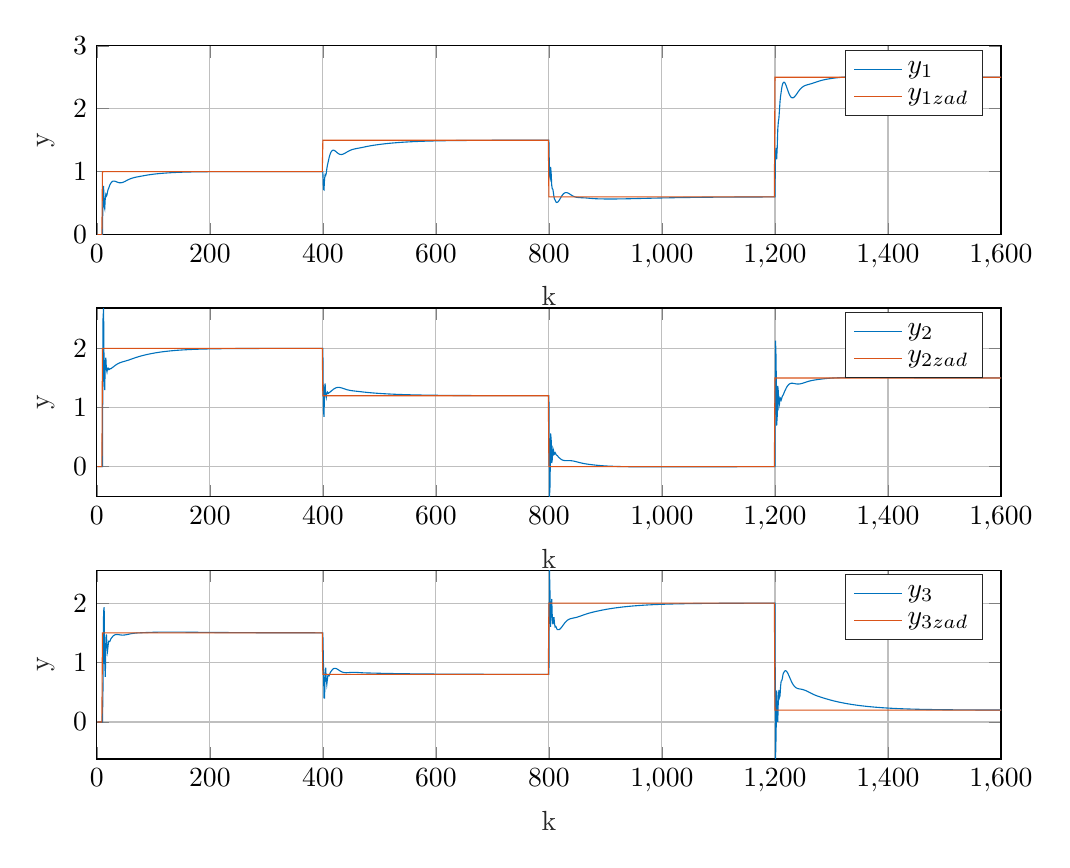
\begin{tikzpicture}

\begin{axis}[%
width=4.521in,
height=0.944in,
at={(0.758in,3.103in)},
scale only axis,
xmin=0,
xmax=1600,
xlabel style={font=\color{white!15!black}},
xlabel={k},
ymin=0,
ymax=3,
ylabel style={font=\color{white!15!black}},
ylabel={y},
axis background/.style={fill=white},
xmajorgrids,
ymajorgrids,
legend style={legend cell align=left, align=left, draw=white!15!black}
]
\addplot [color=mycolor1]
  table[row sep=crcr]{%
1	0\\
2	0\\
3	0\\
4	0\\
5	0\\
6	0\\
7	0\\
8	0\\
9	0\\
10	0\\
11	0.71028\\
12	0.77516\\
13	0.44592\\
14	0.40994\\
15	0.57903\\
16	0.63772\\
17	0.61175\\
18	0.63098\\
19	0.68349\\
20	0.71689\\
21	0.73682\\
22	0.76191\\
23	0.78714\\
24	0.80516\\
25	0.819\\
26	0.83146\\
27	0.84087\\
28	0.84641\\
29	0.84945\\
30	0.85083\\
31	0.85042\\
32	0.84845\\
33	0.84553\\
34	0.84213\\
35	0.83844\\
36	0.83474\\
37	0.83131\\
38	0.82835\\
39	0.826\\
40	0.82435\\
41	0.82348\\
42	0.82342\\
43	0.82414\\
44	0.82562\\
45	0.82781\\
46	0.83062\\
47	0.83397\\
48	0.83777\\
49	0.84193\\
50	0.84635\\
51	0.85095\\
52	0.85563\\
53	0.86032\\
54	0.86496\\
55	0.8695\\
56	0.87388\\
57	0.87808\\
58	0.88206\\
59	0.88582\\
60	0.88934\\
61	0.89264\\
62	0.8957\\
63	0.89856\\
64	0.90122\\
65	0.90369\\
66	0.90601\\
67	0.90819\\
68	0.91025\\
69	0.91221\\
70	0.91409\\
71	0.9159\\
72	0.91767\\
73	0.9194\\
74	0.92111\\
75	0.9228\\
76	0.92448\\
77	0.92615\\
78	0.92782\\
79	0.92949\\
80	0.93115\\
81	0.93281\\
82	0.93446\\
83	0.9361\\
84	0.93772\\
85	0.93933\\
86	0.94092\\
87	0.94249\\
88	0.94402\\
89	0.94553\\
90	0.94701\\
91	0.94845\\
92	0.94985\\
93	0.95122\\
94	0.95256\\
95	0.95385\\
96	0.95511\\
97	0.95633\\
98	0.95752\\
99	0.95867\\
100	0.95979\\
101	0.96088\\
102	0.96194\\
103	0.96297\\
104	0.96397\\
105	0.96494\\
106	0.96589\\
107	0.96682\\
108	0.96772\\
109	0.9686\\
110	0.96947\\
111	0.97031\\
112	0.97113\\
113	0.97194\\
114	0.97272\\
115	0.97349\\
116	0.97425\\
117	0.97498\\
118	0.9757\\
119	0.97641\\
120	0.9771\\
121	0.97777\\
122	0.97843\\
123	0.97907\\
124	0.97969\\
125	0.98031\\
126	0.9809\\
127	0.98149\\
128	0.98205\\
129	0.98261\\
130	0.98315\\
131	0.98367\\
132	0.98419\\
133	0.98469\\
134	0.98518\\
135	0.98565\\
136	0.98611\\
137	0.98656\\
138	0.987\\
139	0.98743\\
140	0.98785\\
141	0.98826\\
142	0.98865\\
143	0.98904\\
144	0.98942\\
145	0.98979\\
146	0.99014\\
147	0.99049\\
148	0.99083\\
149	0.99116\\
150	0.99148\\
151	0.9918\\
152	0.99211\\
153	0.9924\\
154	0.99269\\
155	0.99298\\
156	0.99325\\
157	0.99352\\
158	0.99378\\
159	0.99404\\
160	0.99428\\
161	0.99453\\
162	0.99476\\
163	0.99499\\
164	0.99521\\
165	0.99543\\
166	0.99564\\
167	0.99584\\
168	0.99604\\
169	0.99623\\
170	0.99642\\
171	0.9966\\
172	0.99678\\
173	0.99695\\
174	0.99712\\
175	0.99728\\
176	0.99744\\
177	0.99759\\
178	0.99774\\
179	0.99789\\
180	0.99803\\
181	0.99816\\
182	0.99829\\
183	0.99842\\
184	0.99855\\
185	0.99867\\
186	0.99878\\
187	0.9989\\
188	0.99901\\
189	0.99911\\
190	0.99922\\
191	0.99932\\
192	0.99941\\
193	0.99951\\
194	0.9996\\
195	0.99969\\
196	0.99977\\
197	0.99985\\
198	0.99993\\
199	1\\
200	1.0001\\
201	1.0002\\
202	1.0002\\
203	1.0003\\
204	1.0004\\
205	1.0004\\
206	1.0005\\
207	1.0005\\
208	1.0006\\
209	1.0006\\
210	1.0007\\
211	1.0007\\
212	1.0008\\
213	1.0008\\
214	1.0009\\
215	1.0009\\
216	1.001\\
217	1.001\\
218	1.001\\
219	1.0011\\
220	1.0011\\
221	1.0011\\
222	1.0012\\
223	1.0012\\
224	1.0012\\
225	1.0013\\
226	1.0013\\
227	1.0013\\
228	1.0013\\
229	1.0014\\
230	1.0014\\
231	1.0014\\
232	1.0014\\
233	1.0014\\
234	1.0015\\
235	1.0015\\
236	1.0015\\
237	1.0015\\
238	1.0015\\
239	1.0015\\
240	1.0015\\
241	1.0015\\
242	1.0016\\
243	1.0016\\
244	1.0016\\
245	1.0016\\
246	1.0016\\
247	1.0016\\
248	1.0016\\
249	1.0016\\
250	1.0016\\
251	1.0016\\
252	1.0016\\
253	1.0016\\
254	1.0016\\
255	1.0016\\
256	1.0016\\
257	1.0016\\
258	1.0016\\
259	1.0016\\
260	1.0016\\
261	1.0016\\
262	1.0016\\
263	1.0016\\
264	1.0016\\
265	1.0016\\
266	1.0016\\
267	1.0016\\
268	1.0016\\
269	1.0016\\
270	1.0016\\
271	1.0016\\
272	1.0016\\
273	1.0016\\
274	1.0016\\
275	1.0016\\
276	1.0016\\
277	1.0015\\
278	1.0015\\
279	1.0015\\
280	1.0015\\
281	1.0015\\
282	1.0015\\
283	1.0015\\
284	1.0015\\
285	1.0015\\
286	1.0015\\
287	1.0015\\
288	1.0015\\
289	1.0015\\
290	1.0014\\
291	1.0014\\
292	1.0014\\
293	1.0014\\
294	1.0014\\
295	1.0014\\
296	1.0014\\
297	1.0014\\
298	1.0014\\
299	1.0014\\
300	1.0014\\
301	1.0013\\
302	1.0013\\
303	1.0013\\
304	1.0013\\
305	1.0013\\
306	1.0013\\
307	1.0013\\
308	1.0013\\
309	1.0013\\
310	1.0013\\
311	1.0012\\
312	1.0012\\
313	1.0012\\
314	1.0012\\
315	1.0012\\
316	1.0012\\
317	1.0012\\
318	1.0012\\
319	1.0012\\
320	1.0012\\
321	1.0011\\
322	1.0011\\
323	1.0011\\
324	1.0011\\
325	1.0011\\
326	1.0011\\
327	1.0011\\
328	1.0011\\
329	1.0011\\
330	1.0011\\
331	1.0011\\
332	1.001\\
333	1.001\\
334	1.001\\
335	1.001\\
336	1.001\\
337	1.001\\
338	1.001\\
339	1.001\\
340	1.001\\
341	1.001\\
342	1.001\\
343	1.001\\
344	1.0009\\
345	1.0009\\
346	1.0009\\
347	1.0009\\
348	1.0009\\
349	1.0009\\
350	1.0009\\
351	1.0009\\
352	1.0009\\
353	1.0009\\
354	1.0009\\
355	1.0008\\
356	1.0008\\
357	1.0008\\
358	1.0008\\
359	1.0008\\
360	1.0008\\
361	1.0008\\
362	1.0008\\
363	1.0008\\
364	1.0008\\
365	1.0008\\
366	1.0007\\
367	1.0007\\
368	1.0007\\
369	1.0007\\
370	1.0007\\
371	1.0007\\
372	1.0007\\
373	1.0007\\
374	1.0007\\
375	1.0007\\
376	1.0006\\
377	1.0006\\
378	1.0006\\
379	1.0006\\
380	1.0006\\
381	1.0006\\
382	1.0006\\
383	1.0006\\
384	1.0006\\
385	1.0006\\
386	1.0006\\
387	1.0006\\
388	1.0006\\
389	1.0006\\
390	1.0005\\
391	1.0005\\
392	1.0005\\
393	1.0005\\
394	1.0005\\
395	1.0005\\
396	1.0005\\
397	1.0005\\
398	1.0005\\
399	1.0005\\
400	1.0005\\
401	0.72203\\
402	0.71194\\
403	0.88225\\
404	0.95196\\
405	0.94084\\
406	0.97325\\
407	1.0441\\
408	1.0995\\
409	1.1382\\
410	1.179\\
411	1.2199\\
412	1.2532\\
413	1.2797\\
414	1.3021\\
415	1.3194\\
416	1.331\\
417	1.3381\\
418	1.3415\\
419	1.3415\\
420	1.3387\\
421	1.3337\\
422	1.3273\\
423	1.3199\\
424	1.3121\\
425	1.3043\\
426	1.2969\\
427	1.2903\\
428	1.2845\\
429	1.2799\\
430	1.2764\\
431	1.2742\\
432	1.2732\\
433	1.2734\\
434	1.2747\\
435	1.2769\\
436	1.2801\\
437	1.2839\\
438	1.2883\\
439	1.2931\\
440	1.2982\\
441	1.3035\\
442	1.3089\\
443	1.3142\\
444	1.3194\\
445	1.3244\\
446	1.3291\\
447	1.3336\\
448	1.3378\\
449	1.3416\\
450	1.3452\\
451	1.3485\\
452	1.3514\\
453	1.3542\\
454	1.3567\\
455	1.359\\
456	1.3611\\
457	1.3631\\
458	1.3649\\
459	1.3667\\
460	1.3685\\
461	1.3702\\
462	1.3718\\
463	1.3735\\
464	1.3752\\
465	1.3769\\
466	1.3787\\
467	1.3804\\
468	1.3822\\
469	1.384\\
470	1.3858\\
471	1.3877\\
472	1.3896\\
473	1.3914\\
474	1.3933\\
475	1.3952\\
476	1.397\\
477	1.3989\\
478	1.4007\\
479	1.4025\\
480	1.4042\\
481	1.4059\\
482	1.4076\\
483	1.4093\\
484	1.4109\\
485	1.4125\\
486	1.414\\
487	1.4156\\
488	1.417\\
489	1.4185\\
490	1.4199\\
491	1.4213\\
492	1.4226\\
493	1.424\\
494	1.4253\\
495	1.4265\\
496	1.4278\\
497	1.429\\
498	1.4302\\
499	1.4314\\
500	1.4326\\
501	1.4338\\
502	1.4349\\
503	1.436\\
504	1.4371\\
505	1.4382\\
506	1.4393\\
507	1.4404\\
508	1.4414\\
509	1.4424\\
510	1.4435\\
511	1.4445\\
512	1.4454\\
513	1.4464\\
514	1.4474\\
515	1.4483\\
516	1.4492\\
517	1.4501\\
518	1.451\\
519	1.4519\\
520	1.4527\\
521	1.4536\\
522	1.4544\\
523	1.4552\\
524	1.456\\
525	1.4568\\
526	1.4576\\
527	1.4583\\
528	1.4591\\
529	1.4598\\
530	1.4605\\
531	1.4612\\
532	1.4619\\
533	1.4626\\
534	1.4633\\
535	1.464\\
536	1.4646\\
537	1.4652\\
538	1.4659\\
539	1.4665\\
540	1.4671\\
541	1.4677\\
542	1.4683\\
543	1.4688\\
544	1.4694\\
545	1.47\\
546	1.4705\\
547	1.471\\
548	1.4716\\
549	1.4721\\
550	1.4726\\
551	1.4731\\
552	1.4736\\
553	1.4741\\
554	1.4746\\
555	1.475\\
556	1.4755\\
557	1.4759\\
558	1.4764\\
559	1.4768\\
560	1.4772\\
561	1.4777\\
562	1.4781\\
563	1.4785\\
564	1.4789\\
565	1.4793\\
566	1.4796\\
567	1.48\\
568	1.4804\\
569	1.4808\\
570	1.4811\\
571	1.4815\\
572	1.4818\\
573	1.4821\\
574	1.4825\\
575	1.4828\\
576	1.4831\\
577	1.4834\\
578	1.4838\\
579	1.4841\\
580	1.4844\\
581	1.4846\\
582	1.4849\\
583	1.4852\\
584	1.4855\\
585	1.4858\\
586	1.486\\
587	1.4863\\
588	1.4866\\
589	1.4868\\
590	1.4871\\
591	1.4873\\
592	1.4875\\
593	1.4878\\
594	1.488\\
595	1.4882\\
596	1.4885\\
597	1.4887\\
598	1.4889\\
599	1.4891\\
600	1.4893\\
601	1.4895\\
602	1.4897\\
603	1.4899\\
604	1.4901\\
605	1.4903\\
606	1.4905\\
607	1.4907\\
608	1.4909\\
609	1.491\\
610	1.4912\\
611	1.4914\\
612	1.4915\\
613	1.4917\\
614	1.4919\\
615	1.492\\
616	1.4922\\
617	1.4923\\
618	1.4925\\
619	1.4926\\
620	1.4928\\
621	1.4929\\
622	1.493\\
623	1.4932\\
624	1.4933\\
625	1.4934\\
626	1.4936\\
627	1.4937\\
628	1.4938\\
629	1.4939\\
630	1.4941\\
631	1.4942\\
632	1.4943\\
633	1.4944\\
634	1.4945\\
635	1.4946\\
636	1.4947\\
637	1.4948\\
638	1.4949\\
639	1.495\\
640	1.4951\\
641	1.4952\\
642	1.4953\\
643	1.4954\\
644	1.4955\\
645	1.4956\\
646	1.4957\\
647	1.4958\\
648	1.4959\\
649	1.4959\\
650	1.496\\
651	1.4961\\
652	1.4962\\
653	1.4963\\
654	1.4963\\
655	1.4964\\
656	1.4965\\
657	1.4965\\
658	1.4966\\
659	1.4967\\
660	1.4968\\
661	1.4968\\
662	1.4969\\
663	1.4969\\
664	1.497\\
665	1.4971\\
666	1.4971\\
667	1.4972\\
668	1.4972\\
669	1.4973\\
670	1.4974\\
671	1.4974\\
672	1.4975\\
673	1.4975\\
674	1.4976\\
675	1.4976\\
676	1.4977\\
677	1.4977\\
678	1.4978\\
679	1.4978\\
680	1.4979\\
681	1.4979\\
682	1.4979\\
683	1.498\\
684	1.498\\
685	1.4981\\
686	1.4981\\
687	1.4982\\
688	1.4982\\
689	1.4982\\
690	1.4983\\
691	1.4983\\
692	1.4983\\
693	1.4984\\
694	1.4984\\
695	1.4984\\
696	1.4985\\
697	1.4985\\
698	1.4985\\
699	1.4986\\
700	1.4986\\
701	1.4986\\
702	1.4987\\
703	1.4987\\
704	1.4987\\
705	1.4987\\
706	1.4988\\
707	1.4988\\
708	1.4988\\
709	1.4989\\
710	1.4989\\
711	1.4989\\
712	1.4989\\
713	1.499\\
714	1.499\\
715	1.499\\
716	1.499\\
717	1.499\\
718	1.4991\\
719	1.4991\\
720	1.4991\\
721	1.4991\\
722	1.4991\\
723	1.4992\\
724	1.4992\\
725	1.4992\\
726	1.4992\\
727	1.4992\\
728	1.4993\\
729	1.4993\\
730	1.4993\\
731	1.4993\\
732	1.4993\\
733	1.4993\\
734	1.4994\\
735	1.4994\\
736	1.4994\\
737	1.4994\\
738	1.4994\\
739	1.4994\\
740	1.4994\\
741	1.4995\\
742	1.4995\\
743	1.4995\\
744	1.4995\\
745	1.4995\\
746	1.4995\\
747	1.4995\\
748	1.4995\\
749	1.4996\\
750	1.4996\\
751	1.4996\\
752	1.4996\\
753	1.4996\\
754	1.4996\\
755	1.4996\\
756	1.4996\\
757	1.4996\\
758	1.4996\\
759	1.4997\\
760	1.4997\\
761	1.4997\\
762	1.4997\\
763	1.4997\\
764	1.4997\\
765	1.4997\\
766	1.4997\\
767	1.4997\\
768	1.4997\\
769	1.4997\\
770	1.4997\\
771	1.4997\\
772	1.4997\\
773	1.4997\\
774	1.4997\\
775	1.4998\\
776	1.4998\\
777	1.4998\\
778	1.4998\\
779	1.4998\\
780	1.4998\\
781	1.4998\\
782	1.4998\\
783	1.4998\\
784	1.4998\\
785	1.4998\\
786	1.4998\\
787	1.4998\\
788	1.4998\\
789	1.4998\\
790	1.4998\\
791	1.4998\\
792	1.4999\\
793	1.4999\\
794	1.4999\\
795	1.4999\\
796	1.4999\\
797	1.4999\\
798	1.4999\\
799	1.4999\\
800	1.4999\\
801	0.94926\\
802	0.90325\\
803	1.0749\\
804	0.97495\\
805	0.78213\\
806	0.72758\\
807	0.72193\\
808	0.66328\\
809	0.59603\\
810	0.56459\\
811	0.54819\\
812	0.52826\\
813	0.5138\\
814	0.51103\\
815	0.51436\\
816	0.52015\\
817	0.52964\\
818	0.54279\\
819	0.55758\\
820	0.57283\\
821	0.58834\\
822	0.60358\\
823	0.61776\\
824	0.63047\\
825	0.64151\\
826	0.65072\\
827	0.65793\\
828	0.66314\\
829	0.66643\\
830	0.66792\\
831	0.66776\\
832	0.66614\\
833	0.66329\\
834	0.65942\\
835	0.65477\\
836	0.64955\\
837	0.64396\\
838	0.6382\\
839	0.63242\\
840	0.62677\\
841	0.62137\\
842	0.6163\\
843	0.61163\\
844	0.60741\\
845	0.60365\\
846	0.60037\\
847	0.59755\\
848	0.59516\\
849	0.59318\\
850	0.59156\\
851	0.59026\\
852	0.58923\\
853	0.58842\\
854	0.58779\\
855	0.58728\\
856	0.58687\\
857	0.5865\\
858	0.58616\\
859	0.58582\\
860	0.58545\\
861	0.58504\\
862	0.58459\\
863	0.58407\\
864	0.58351\\
865	0.58288\\
866	0.5822\\
867	0.58148\\
868	0.58072\\
869	0.57993\\
870	0.57912\\
871	0.57831\\
872	0.57749\\
873	0.57668\\
874	0.57588\\
875	0.57511\\
876	0.57437\\
877	0.57366\\
878	0.57298\\
879	0.57235\\
880	0.57176\\
881	0.57122\\
882	0.57071\\
883	0.57024\\
884	0.56982\\
885	0.56943\\
886	0.56908\\
887	0.56876\\
888	0.56847\\
889	0.56821\\
890	0.56798\\
891	0.56776\\
892	0.56757\\
893	0.5674\\
894	0.56724\\
895	0.56709\\
896	0.56696\\
897	0.56684\\
898	0.56673\\
899	0.56664\\
900	0.56655\\
901	0.56647\\
902	0.5664\\
903	0.56634\\
904	0.56629\\
905	0.56625\\
906	0.56621\\
907	0.56619\\
908	0.56618\\
909	0.56617\\
910	0.56618\\
911	0.56619\\
912	0.56622\\
913	0.56625\\
914	0.56629\\
915	0.56634\\
916	0.56641\\
917	0.56648\\
918	0.56655\\
919	0.56664\\
920	0.56674\\
921	0.56684\\
922	0.56695\\
923	0.56706\\
924	0.56719\\
925	0.56732\\
926	0.56745\\
927	0.56759\\
928	0.56774\\
929	0.56789\\
930	0.56804\\
931	0.5682\\
932	0.56837\\
933	0.56854\\
934	0.56871\\
935	0.56888\\
936	0.56906\\
937	0.56924\\
938	0.56943\\
939	0.56962\\
940	0.56981\\
941	0.57\\
942	0.5702\\
943	0.5704\\
944	0.5706\\
945	0.5708\\
946	0.57101\\
947	0.57121\\
948	0.57142\\
949	0.57163\\
950	0.57184\\
951	0.57206\\
952	0.57227\\
953	0.57249\\
954	0.5727\\
955	0.57292\\
956	0.57314\\
957	0.57336\\
958	0.57358\\
959	0.5738\\
960	0.57402\\
961	0.57425\\
962	0.57447\\
963	0.57469\\
964	0.57492\\
965	0.57514\\
966	0.57536\\
967	0.57559\\
968	0.57581\\
969	0.57603\\
970	0.57625\\
971	0.57648\\
972	0.5767\\
973	0.57692\\
974	0.57714\\
975	0.57736\\
976	0.57758\\
977	0.5778\\
978	0.57802\\
979	0.57824\\
980	0.57846\\
981	0.57868\\
982	0.57889\\
983	0.57911\\
984	0.57932\\
985	0.57954\\
986	0.57975\\
987	0.57996\\
988	0.58017\\
989	0.58038\\
990	0.58059\\
991	0.5808\\
992	0.581\\
993	0.58121\\
994	0.58141\\
995	0.58161\\
996	0.58181\\
997	0.58202\\
998	0.58221\\
999	0.58241\\
1000	0.58261\\
1001	0.5828\\
1002	0.583\\
1003	0.58319\\
1004	0.58338\\
1005	0.58357\\
1006	0.58376\\
1007	0.58394\\
1008	0.58413\\
1009	0.58431\\
1010	0.5845\\
1011	0.58468\\
1012	0.58486\\
1013	0.58504\\
1014	0.58521\\
1015	0.58539\\
1016	0.58556\\
1017	0.58573\\
1018	0.58591\\
1019	0.58608\\
1020	0.58624\\
1021	0.58641\\
1022	0.58658\\
1023	0.58674\\
1024	0.5869\\
1025	0.58706\\
1026	0.58722\\
1027	0.58738\\
1028	0.58754\\
1029	0.58769\\
1030	0.58784\\
1031	0.588\\
1032	0.58815\\
1033	0.58829\\
1034	0.58844\\
1035	0.58859\\
1036	0.58873\\
1037	0.58888\\
1038	0.58902\\
1039	0.58916\\
1040	0.5893\\
1041	0.58943\\
1042	0.58957\\
1043	0.58971\\
1044	0.58984\\
1045	0.58997\\
1046	0.5901\\
1047	0.59023\\
1048	0.59036\\
1049	0.59048\\
1050	0.59061\\
1051	0.59073\\
1052	0.59085\\
1053	0.59098\\
1054	0.5911\\
1055	0.59121\\
1056	0.59133\\
1057	0.59145\\
1058	0.59156\\
1059	0.59167\\
1060	0.59178\\
1061	0.5919\\
1062	0.592\\
1063	0.59211\\
1064	0.59222\\
1065	0.59232\\
1066	0.59243\\
1067	0.59253\\
1068	0.59263\\
1069	0.59273\\
1070	0.59283\\
1071	0.59293\\
1072	0.59303\\
1073	0.59312\\
1074	0.59322\\
1075	0.59331\\
1076	0.5934\\
1077	0.5935\\
1078	0.59359\\
1079	0.59368\\
1080	0.59376\\
1081	0.59385\\
1082	0.59394\\
1083	0.59402\\
1084	0.5941\\
1085	0.59419\\
1086	0.59427\\
1087	0.59435\\
1088	0.59443\\
1089	0.59451\\
1090	0.59458\\
1091	0.59466\\
1092	0.59474\\
1093	0.59481\\
1094	0.59488\\
1095	0.59496\\
1096	0.59503\\
1097	0.5951\\
1098	0.59517\\
1099	0.59524\\
1100	0.59531\\
1101	0.59537\\
1102	0.59544\\
1103	0.5955\\
1104	0.59557\\
1105	0.59563\\
1106	0.59569\\
1107	0.59576\\
1108	0.59582\\
1109	0.59588\\
1110	0.59594\\
1111	0.596\\
1112	0.59605\\
1113	0.59611\\
1114	0.59617\\
1115	0.59622\\
1116	0.59628\\
1117	0.59633\\
1118	0.59638\\
1119	0.59644\\
1120	0.59649\\
1121	0.59654\\
1122	0.59659\\
1123	0.59664\\
1124	0.59669\\
1125	0.59674\\
1126	0.59678\\
1127	0.59683\\
1128	0.59688\\
1129	0.59692\\
1130	0.59697\\
1131	0.59701\\
1132	0.59706\\
1133	0.5971\\
1134	0.59714\\
1135	0.59718\\
1136	0.59723\\
1137	0.59727\\
1138	0.59731\\
1139	0.59735\\
1140	0.59739\\
1141	0.59743\\
1142	0.59747\\
1143	0.59751\\
1144	0.59754\\
1145	0.59758\\
1146	0.59762\\
1147	0.59765\\
1148	0.59769\\
1149	0.59773\\
1150	0.59776\\
1151	0.5978\\
1152	0.59783\\
1153	0.59786\\
1154	0.5979\\
1155	0.59793\\
1156	0.59796\\
1157	0.598\\
1158	0.59803\\
1159	0.59806\\
1160	0.5981\\
1161	0.59813\\
1162	0.59816\\
1163	0.59819\\
1164	0.59823\\
1165	0.59826\\
1166	0.59829\\
1167	0.59832\\
1168	0.59834\\
1169	0.59837\\
1170	0.5984\\
1171	0.59842\\
1172	0.59845\\
1173	0.59847\\
1174	0.5985\\
1175	0.59852\\
1176	0.59854\\
1177	0.59856\\
1178	0.59858\\
1179	0.59861\\
1180	0.59863\\
1181	0.59865\\
1182	0.59867\\
1183	0.59869\\
1184	0.59871\\
1185	0.59873\\
1186	0.59875\\
1187	0.59877\\
1188	0.59879\\
1189	0.59881\\
1190	0.59883\\
1191	0.59884\\
1192	0.59886\\
1193	0.59888\\
1194	0.5989\\
1195	0.59892\\
1196	0.59894\\
1197	0.59896\\
1198	0.59897\\
1199	0.59899\\
1200	0.59901\\
1201	1.3049\\
1202	1.3762\\
1203	1.1964\\
1204	1.3796\\
1205	1.6768\\
1206	1.7932\\
1207	1.8525\\
1208	1.9829\\
1209	2.12\\
1210	2.2052\\
1211	2.2667\\
1212	2.3279\\
1213	2.3762\\
1214	2.4032\\
1215	2.4168\\
1216	2.422\\
1217	2.4175\\
1218	2.404\\
1219	2.3849\\
1220	2.3622\\
1221	2.337\\
1222	2.3106\\
1223	2.2846\\
1224	2.26\\
1225	2.2377\\
1226	2.2181\\
1227	2.2019\\
1228	2.1894\\
1229	2.1805\\
1230	2.1752\\
1231	2.1733\\
1232	2.1747\\
1233	2.1789\\
1234	2.1856\\
1235	2.1944\\
1236	2.2048\\
1237	2.2164\\
1238	2.2289\\
1239	2.2419\\
1240	2.2549\\
1241	2.2679\\
1242	2.2804\\
1243	2.2924\\
1244	2.3037\\
1245	2.3141\\
1246	2.3237\\
1247	2.3323\\
1248	2.3401\\
1249	2.347\\
1250	2.3531\\
1251	2.3584\\
1252	2.3631\\
1253	2.3673\\
1254	2.3709\\
1255	2.3742\\
1256	2.3771\\
1257	2.3798\\
1258	2.3824\\
1259	2.3849\\
1260	2.3873\\
1261	2.3898\\
1262	2.3923\\
1263	2.3949\\
1264	2.3975\\
1265	2.4002\\
1266	2.403\\
1267	2.4059\\
1268	2.4089\\
1269	2.4119\\
1270	2.415\\
1271	2.418\\
1272	2.4211\\
1273	2.4242\\
1274	2.4273\\
1275	2.4303\\
1276	2.4333\\
1277	2.4362\\
1278	2.439\\
1279	2.4418\\
1280	2.4444\\
1281	2.447\\
1282	2.4495\\
1283	2.4518\\
1284	2.4541\\
1285	2.4563\\
1286	2.4584\\
1287	2.4604\\
1288	2.4624\\
1289	2.4642\\
1290	2.466\\
1291	2.4677\\
1292	2.4694\\
1293	2.471\\
1294	2.4726\\
1295	2.4741\\
1296	2.4756\\
1297	2.477\\
1298	2.4784\\
1299	2.4798\\
1300	2.4811\\
1301	2.4824\\
1302	2.4837\\
1303	2.4849\\
1304	2.4861\\
1305	2.4873\\
1306	2.4884\\
1307	2.4895\\
1308	2.4906\\
1309	2.4917\\
1310	2.4927\\
1311	2.4937\\
1312	2.4946\\
1313	2.4956\\
1314	2.4965\\
1315	2.4973\\
1316	2.4982\\
1317	2.499\\
1318	2.4998\\
1319	2.5005\\
1320	2.5012\\
1321	2.502\\
1322	2.5026\\
1323	2.5033\\
1324	2.5039\\
1325	2.5045\\
1326	2.5051\\
1327	2.5057\\
1328	2.5062\\
1329	2.5067\\
1330	2.5072\\
1331	2.5077\\
1332	2.5082\\
1333	2.5086\\
1334	2.509\\
1335	2.5094\\
1336	2.5098\\
1337	2.5102\\
1338	2.5106\\
1339	2.5109\\
1340	2.5112\\
1341	2.5116\\
1342	2.5119\\
1343	2.5122\\
1344	2.5124\\
1345	2.5127\\
1346	2.5129\\
1347	2.5132\\
1348	2.5134\\
1349	2.5136\\
1350	2.5138\\
1351	2.514\\
1352	2.5142\\
1353	2.5144\\
1354	2.5145\\
1355	2.5147\\
1356	2.5148\\
1357	2.515\\
1358	2.5151\\
1359	2.5152\\
1360	2.5153\\
1361	2.5154\\
1362	2.5155\\
1363	2.5156\\
1364	2.5156\\
1365	2.5157\\
1366	2.5158\\
1367	2.5158\\
1368	2.5159\\
1369	2.5159\\
1370	2.5159\\
1371	2.516\\
1372	2.516\\
1373	2.516\\
1374	2.516\\
1375	2.516\\
1376	2.516\\
1377	2.516\\
1378	2.516\\
1379	2.516\\
1380	2.516\\
1381	2.5159\\
1382	2.5159\\
1383	2.5159\\
1384	2.5158\\
1385	2.5158\\
1386	2.5158\\
1387	2.5157\\
1388	2.5157\\
1389	2.5156\\
1390	2.5156\\
1391	2.5155\\
1392	2.5154\\
1393	2.5154\\
1394	2.5153\\
1395	2.5152\\
1396	2.5152\\
1397	2.5151\\
1398	2.515\\
1399	2.5149\\
1400	2.5149\\
1401	2.5148\\
1402	2.5147\\
1403	2.5146\\
1404	2.5145\\
1405	2.5144\\
1406	2.5143\\
1407	2.5143\\
1408	2.5142\\
1409	2.5141\\
1410	2.514\\
1411	2.5139\\
1412	2.5138\\
1413	2.5137\\
1414	2.5136\\
1415	2.5135\\
1416	2.5134\\
1417	2.5133\\
1418	2.5132\\
1419	2.5131\\
1420	2.513\\
1421	2.5129\\
1422	2.5128\\
1423	2.5127\\
1424	2.5126\\
1425	2.5125\\
1426	2.5124\\
1427	2.5123\\
1428	2.5121\\
1429	2.512\\
1430	2.5119\\
1431	2.5118\\
1432	2.5117\\
1433	2.5116\\
1434	2.5115\\
1435	2.5114\\
1436	2.5113\\
1437	2.5112\\
1438	2.5111\\
1439	2.511\\
1440	2.5109\\
1441	2.5108\\
1442	2.5107\\
1443	2.5106\\
1444	2.5105\\
1445	2.5104\\
1446	2.5103\\
1447	2.5102\\
1448	2.51\\
1449	2.5099\\
1450	2.5098\\
1451	2.5097\\
1452	2.5096\\
1453	2.5095\\
1454	2.5094\\
1455	2.5093\\
1456	2.5092\\
1457	2.5091\\
1458	2.509\\
1459	2.5089\\
1460	2.5089\\
1461	2.5088\\
1462	2.5087\\
1463	2.5086\\
1464	2.5085\\
1465	2.5084\\
1466	2.5083\\
1467	2.5082\\
1468	2.5081\\
1469	2.508\\
1470	2.5079\\
1471	2.5078\\
1472	2.5077\\
1473	2.5077\\
1474	2.5076\\
1475	2.5075\\
1476	2.5074\\
1477	2.5073\\
1478	2.5072\\
1479	2.5071\\
1480	2.5071\\
1481	2.507\\
1482	2.5069\\
1483	2.5068\\
1484	2.5067\\
1485	2.5066\\
1486	2.5066\\
1487	2.5065\\
1488	2.5064\\
1489	2.5063\\
1490	2.5063\\
1491	2.5062\\
1492	2.5061\\
1493	2.506\\
1494	2.506\\
1495	2.5059\\
1496	2.5058\\
1497	2.5057\\
1498	2.5057\\
1499	2.5056\\
1500	2.5055\\
1501	2.5055\\
1502	2.5054\\
1503	2.5053\\
1504	2.5053\\
1505	2.5052\\
1506	2.5051\\
1507	2.5051\\
1508	2.505\\
1509	2.5049\\
1510	2.5049\\
1511	2.5048\\
1512	2.5048\\
1513	2.5047\\
1514	2.5046\\
1515	2.5046\\
1516	2.5045\\
1517	2.5045\\
1518	2.5044\\
1519	2.5044\\
1520	2.5043\\
1521	2.5042\\
1522	2.5042\\
1523	2.5041\\
1524	2.5041\\
1525	2.504\\
1526	2.504\\
1527	2.5039\\
1528	2.5039\\
1529	2.5038\\
1530	2.5038\\
1531	2.5037\\
1532	2.5037\\
1533	2.5036\\
1534	2.5036\\
1535	2.5035\\
1536	2.5035\\
1537	2.5034\\
1538	2.5034\\
1539	2.5034\\
1540	2.5033\\
1541	2.5033\\
1542	2.5032\\
1543	2.5032\\
1544	2.5031\\
1545	2.5031\\
1546	2.5031\\
1547	2.503\\
1548	2.503\\
1549	2.5029\\
1550	2.5029\\
1551	2.5028\\
1552	2.5028\\
1553	2.5028\\
1554	2.5027\\
1555	2.5027\\
1556	2.5027\\
1557	2.5026\\
1558	2.5026\\
1559	2.5025\\
1560	2.5025\\
1561	2.5024\\
1562	2.5024\\
1563	2.5024\\
1564	2.5023\\
1565	2.5023\\
1566	2.5022\\
1567	2.5022\\
1568	2.5022\\
1569	2.5021\\
1570	2.5021\\
1571	2.5021\\
1572	2.502\\
1573	2.502\\
1574	2.502\\
1575	2.502\\
1576	2.5019\\
1577	2.5019\\
1578	2.5019\\
1579	2.5019\\
1580	2.5018\\
1581	2.5018\\
1582	2.5018\\
1583	2.5018\\
1584	2.5017\\
1585	2.5017\\
1586	2.5017\\
1587	2.5017\\
1588	2.5016\\
1589	2.5016\\
1590	2.5016\\
1591	2.5016\\
1592	2.5015\\
1593	2.5015\\
1594	2.5015\\
1595	2.5015\\
1596	2.5014\\
1597	2.5014\\
1598	2.5014\\
1599	2.5014\\
1600	2.5014\\
};
\addlegendentry{$\text{y}_\text{1}$}

\addplot [color=mycolor2]
  table[row sep=crcr]{%
1	0\\
2	0\\
3	0\\
4	0\\
5	0\\
6	0\\
7	0\\
8	0\\
9	0\\
10	1\\
11	1\\
12	1\\
13	1\\
14	1\\
15	1\\
16	1\\
17	1\\
18	1\\
19	1\\
20	1\\
21	1\\
22	1\\
23	1\\
24	1\\
25	1\\
26	1\\
27	1\\
28	1\\
29	1\\
30	1\\
31	1\\
32	1\\
33	1\\
34	1\\
35	1\\
36	1\\
37	1\\
38	1\\
39	1\\
40	1\\
41	1\\
42	1\\
43	1\\
44	1\\
45	1\\
46	1\\
47	1\\
48	1\\
49	1\\
50	1\\
51	1\\
52	1\\
53	1\\
54	1\\
55	1\\
56	1\\
57	1\\
58	1\\
59	1\\
60	1\\
61	1\\
62	1\\
63	1\\
64	1\\
65	1\\
66	1\\
67	1\\
68	1\\
69	1\\
70	1\\
71	1\\
72	1\\
73	1\\
74	1\\
75	1\\
76	1\\
77	1\\
78	1\\
79	1\\
80	1\\
81	1\\
82	1\\
83	1\\
84	1\\
85	1\\
86	1\\
87	1\\
88	1\\
89	1\\
90	1\\
91	1\\
92	1\\
93	1\\
94	1\\
95	1\\
96	1\\
97	1\\
98	1\\
99	1\\
100	1\\
101	1\\
102	1\\
103	1\\
104	1\\
105	1\\
106	1\\
107	1\\
108	1\\
109	1\\
110	1\\
111	1\\
112	1\\
113	1\\
114	1\\
115	1\\
116	1\\
117	1\\
118	1\\
119	1\\
120	1\\
121	1\\
122	1\\
123	1\\
124	1\\
125	1\\
126	1\\
127	1\\
128	1\\
129	1\\
130	1\\
131	1\\
132	1\\
133	1\\
134	1\\
135	1\\
136	1\\
137	1\\
138	1\\
139	1\\
140	1\\
141	1\\
142	1\\
143	1\\
144	1\\
145	1\\
146	1\\
147	1\\
148	1\\
149	1\\
150	1\\
151	1\\
152	1\\
153	1\\
154	1\\
155	1\\
156	1\\
157	1\\
158	1\\
159	1\\
160	1\\
161	1\\
162	1\\
163	1\\
164	1\\
165	1\\
166	1\\
167	1\\
168	1\\
169	1\\
170	1\\
171	1\\
172	1\\
173	1\\
174	1\\
175	1\\
176	1\\
177	1\\
178	1\\
179	1\\
180	1\\
181	1\\
182	1\\
183	1\\
184	1\\
185	1\\
186	1\\
187	1\\
188	1\\
189	1\\
190	1\\
191	1\\
192	1\\
193	1\\
194	1\\
195	1\\
196	1\\
197	1\\
198	1\\
199	1\\
200	1\\
201	1\\
202	1\\
203	1\\
204	1\\
205	1\\
206	1\\
207	1\\
208	1\\
209	1\\
210	1\\
211	1\\
212	1\\
213	1\\
214	1\\
215	1\\
216	1\\
217	1\\
218	1\\
219	1\\
220	1\\
221	1\\
222	1\\
223	1\\
224	1\\
225	1\\
226	1\\
227	1\\
228	1\\
229	1\\
230	1\\
231	1\\
232	1\\
233	1\\
234	1\\
235	1\\
236	1\\
237	1\\
238	1\\
239	1\\
240	1\\
241	1\\
242	1\\
243	1\\
244	1\\
245	1\\
246	1\\
247	1\\
248	1\\
249	1\\
250	1\\
251	1\\
252	1\\
253	1\\
254	1\\
255	1\\
256	1\\
257	1\\
258	1\\
259	1\\
260	1\\
261	1\\
262	1\\
263	1\\
264	1\\
265	1\\
266	1\\
267	1\\
268	1\\
269	1\\
270	1\\
271	1\\
272	1\\
273	1\\
274	1\\
275	1\\
276	1\\
277	1\\
278	1\\
279	1\\
280	1\\
281	1\\
282	1\\
283	1\\
284	1\\
285	1\\
286	1\\
287	1\\
288	1\\
289	1\\
290	1\\
291	1\\
292	1\\
293	1\\
294	1\\
295	1\\
296	1\\
297	1\\
298	1\\
299	1\\
300	1\\
301	1\\
302	1\\
303	1\\
304	1\\
305	1\\
306	1\\
307	1\\
308	1\\
309	1\\
310	1\\
311	1\\
312	1\\
313	1\\
314	1\\
315	1\\
316	1\\
317	1\\
318	1\\
319	1\\
320	1\\
321	1\\
322	1\\
323	1\\
324	1\\
325	1\\
326	1\\
327	1\\
328	1\\
329	1\\
330	1\\
331	1\\
332	1\\
333	1\\
334	1\\
335	1\\
336	1\\
337	1\\
338	1\\
339	1\\
340	1\\
341	1\\
342	1\\
343	1\\
344	1\\
345	1\\
346	1\\
347	1\\
348	1\\
349	1\\
350	1\\
351	1\\
352	1\\
353	1\\
354	1\\
355	1\\
356	1\\
357	1\\
358	1\\
359	1\\
360	1\\
361	1\\
362	1\\
363	1\\
364	1\\
365	1\\
366	1\\
367	1\\
368	1\\
369	1\\
370	1\\
371	1\\
372	1\\
373	1\\
374	1\\
375	1\\
376	1\\
377	1\\
378	1\\
379	1\\
380	1\\
381	1\\
382	1\\
383	1\\
384	1\\
385	1\\
386	1\\
387	1\\
388	1\\
389	1\\
390	1\\
391	1\\
392	1\\
393	1\\
394	1\\
395	1\\
396	1\\
397	1\\
398	1\\
399	1\\
400	1.5\\
401	1.5\\
402	1.5\\
403	1.5\\
404	1.5\\
405	1.5\\
406	1.5\\
407	1.5\\
408	1.5\\
409	1.5\\
410	1.5\\
411	1.5\\
412	1.5\\
413	1.5\\
414	1.5\\
415	1.5\\
416	1.5\\
417	1.5\\
418	1.5\\
419	1.5\\
420	1.5\\
421	1.5\\
422	1.5\\
423	1.5\\
424	1.5\\
425	1.5\\
426	1.5\\
427	1.5\\
428	1.5\\
429	1.5\\
430	1.5\\
431	1.5\\
432	1.5\\
433	1.5\\
434	1.5\\
435	1.5\\
436	1.5\\
437	1.5\\
438	1.5\\
439	1.5\\
440	1.5\\
441	1.5\\
442	1.5\\
443	1.5\\
444	1.5\\
445	1.5\\
446	1.5\\
447	1.5\\
448	1.5\\
449	1.5\\
450	1.5\\
451	1.5\\
452	1.5\\
453	1.5\\
454	1.5\\
455	1.5\\
456	1.5\\
457	1.5\\
458	1.5\\
459	1.5\\
460	1.5\\
461	1.5\\
462	1.5\\
463	1.5\\
464	1.5\\
465	1.5\\
466	1.5\\
467	1.5\\
468	1.5\\
469	1.5\\
470	1.5\\
471	1.5\\
472	1.5\\
473	1.5\\
474	1.5\\
475	1.5\\
476	1.5\\
477	1.5\\
478	1.5\\
479	1.5\\
480	1.5\\
481	1.5\\
482	1.5\\
483	1.5\\
484	1.5\\
485	1.5\\
486	1.5\\
487	1.5\\
488	1.5\\
489	1.5\\
490	1.5\\
491	1.5\\
492	1.5\\
493	1.5\\
494	1.5\\
495	1.5\\
496	1.5\\
497	1.5\\
498	1.5\\
499	1.5\\
500	1.5\\
501	1.5\\
502	1.5\\
503	1.5\\
504	1.5\\
505	1.5\\
506	1.5\\
507	1.5\\
508	1.5\\
509	1.5\\
510	1.5\\
511	1.5\\
512	1.5\\
513	1.5\\
514	1.5\\
515	1.5\\
516	1.5\\
517	1.5\\
518	1.5\\
519	1.5\\
520	1.5\\
521	1.5\\
522	1.5\\
523	1.5\\
524	1.5\\
525	1.5\\
526	1.5\\
527	1.5\\
528	1.5\\
529	1.5\\
530	1.5\\
531	1.5\\
532	1.5\\
533	1.5\\
534	1.5\\
535	1.5\\
536	1.5\\
537	1.5\\
538	1.5\\
539	1.5\\
540	1.5\\
541	1.5\\
542	1.5\\
543	1.5\\
544	1.5\\
545	1.5\\
546	1.5\\
547	1.5\\
548	1.5\\
549	1.5\\
550	1.5\\
551	1.5\\
552	1.5\\
553	1.5\\
554	1.5\\
555	1.5\\
556	1.5\\
557	1.5\\
558	1.5\\
559	1.5\\
560	1.5\\
561	1.5\\
562	1.5\\
563	1.5\\
564	1.5\\
565	1.5\\
566	1.5\\
567	1.5\\
568	1.5\\
569	1.5\\
570	1.5\\
571	1.5\\
572	1.5\\
573	1.5\\
574	1.5\\
575	1.5\\
576	1.5\\
577	1.5\\
578	1.5\\
579	1.5\\
580	1.5\\
581	1.5\\
582	1.5\\
583	1.5\\
584	1.5\\
585	1.5\\
586	1.5\\
587	1.5\\
588	1.5\\
589	1.5\\
590	1.5\\
591	1.5\\
592	1.5\\
593	1.5\\
594	1.5\\
595	1.5\\
596	1.5\\
597	1.5\\
598	1.5\\
599	1.5\\
600	1.5\\
601	1.5\\
602	1.5\\
603	1.5\\
604	1.5\\
605	1.5\\
606	1.5\\
607	1.5\\
608	1.5\\
609	1.5\\
610	1.5\\
611	1.5\\
612	1.5\\
613	1.5\\
614	1.5\\
615	1.5\\
616	1.5\\
617	1.5\\
618	1.5\\
619	1.5\\
620	1.5\\
621	1.5\\
622	1.5\\
623	1.5\\
624	1.5\\
625	1.5\\
626	1.5\\
627	1.5\\
628	1.5\\
629	1.5\\
630	1.5\\
631	1.5\\
632	1.5\\
633	1.5\\
634	1.5\\
635	1.5\\
636	1.5\\
637	1.5\\
638	1.5\\
639	1.5\\
640	1.5\\
641	1.5\\
642	1.5\\
643	1.5\\
644	1.5\\
645	1.5\\
646	1.5\\
647	1.5\\
648	1.5\\
649	1.5\\
650	1.5\\
651	1.5\\
652	1.5\\
653	1.5\\
654	1.5\\
655	1.5\\
656	1.5\\
657	1.5\\
658	1.5\\
659	1.5\\
660	1.5\\
661	1.5\\
662	1.5\\
663	1.5\\
664	1.5\\
665	1.5\\
666	1.5\\
667	1.5\\
668	1.5\\
669	1.5\\
670	1.5\\
671	1.5\\
672	1.5\\
673	1.5\\
674	1.5\\
675	1.5\\
676	1.5\\
677	1.5\\
678	1.5\\
679	1.5\\
680	1.5\\
681	1.5\\
682	1.5\\
683	1.5\\
684	1.5\\
685	1.5\\
686	1.5\\
687	1.5\\
688	1.5\\
689	1.5\\
690	1.5\\
691	1.5\\
692	1.5\\
693	1.5\\
694	1.5\\
695	1.5\\
696	1.5\\
697	1.5\\
698	1.5\\
699	1.5\\
700	1.5\\
701	1.5\\
702	1.5\\
703	1.5\\
704	1.5\\
705	1.5\\
706	1.5\\
707	1.5\\
708	1.5\\
709	1.5\\
710	1.5\\
711	1.5\\
712	1.5\\
713	1.5\\
714	1.5\\
715	1.5\\
716	1.5\\
717	1.5\\
718	1.5\\
719	1.5\\
720	1.5\\
721	1.5\\
722	1.5\\
723	1.5\\
724	1.5\\
725	1.5\\
726	1.5\\
727	1.5\\
728	1.5\\
729	1.5\\
730	1.5\\
731	1.5\\
732	1.5\\
733	1.5\\
734	1.5\\
735	1.5\\
736	1.5\\
737	1.5\\
738	1.5\\
739	1.5\\
740	1.5\\
741	1.5\\
742	1.5\\
743	1.5\\
744	1.5\\
745	1.5\\
746	1.5\\
747	1.5\\
748	1.5\\
749	1.5\\
750	1.5\\
751	1.5\\
752	1.5\\
753	1.5\\
754	1.5\\
755	1.5\\
756	1.5\\
757	1.5\\
758	1.5\\
759	1.5\\
760	1.5\\
761	1.5\\
762	1.5\\
763	1.5\\
764	1.5\\
765	1.5\\
766	1.5\\
767	1.5\\
768	1.5\\
769	1.5\\
770	1.5\\
771	1.5\\
772	1.5\\
773	1.5\\
774	1.5\\
775	1.5\\
776	1.5\\
777	1.5\\
778	1.5\\
779	1.5\\
780	1.5\\
781	1.5\\
782	1.5\\
783	1.5\\
784	1.5\\
785	1.5\\
786	1.5\\
787	1.5\\
788	1.5\\
789	1.5\\
790	1.5\\
791	1.5\\
792	1.5\\
793	1.5\\
794	1.5\\
795	1.5\\
796	1.5\\
797	1.5\\
798	1.5\\
799	1.5\\
800	0.6\\
801	0.6\\
802	0.6\\
803	0.6\\
804	0.6\\
805	0.6\\
806	0.6\\
807	0.6\\
808	0.6\\
809	0.6\\
810	0.6\\
811	0.6\\
812	0.6\\
813	0.6\\
814	0.6\\
815	0.6\\
816	0.6\\
817	0.6\\
818	0.6\\
819	0.6\\
820	0.6\\
821	0.6\\
822	0.6\\
823	0.6\\
824	0.6\\
825	0.6\\
826	0.6\\
827	0.6\\
828	0.6\\
829	0.6\\
830	0.6\\
831	0.6\\
832	0.6\\
833	0.6\\
834	0.6\\
835	0.6\\
836	0.6\\
837	0.6\\
838	0.6\\
839	0.6\\
840	0.6\\
841	0.6\\
842	0.6\\
843	0.6\\
844	0.6\\
845	0.6\\
846	0.6\\
847	0.6\\
848	0.6\\
849	0.6\\
850	0.6\\
851	0.6\\
852	0.6\\
853	0.6\\
854	0.6\\
855	0.6\\
856	0.6\\
857	0.6\\
858	0.6\\
859	0.6\\
860	0.6\\
861	0.6\\
862	0.6\\
863	0.6\\
864	0.6\\
865	0.6\\
866	0.6\\
867	0.6\\
868	0.6\\
869	0.6\\
870	0.6\\
871	0.6\\
872	0.6\\
873	0.6\\
874	0.6\\
875	0.6\\
876	0.6\\
877	0.6\\
878	0.6\\
879	0.6\\
880	0.6\\
881	0.6\\
882	0.6\\
883	0.6\\
884	0.6\\
885	0.6\\
886	0.6\\
887	0.6\\
888	0.6\\
889	0.6\\
890	0.6\\
891	0.6\\
892	0.6\\
893	0.6\\
894	0.6\\
895	0.6\\
896	0.6\\
897	0.6\\
898	0.6\\
899	0.6\\
900	0.6\\
901	0.6\\
902	0.6\\
903	0.6\\
904	0.6\\
905	0.6\\
906	0.6\\
907	0.6\\
908	0.6\\
909	0.6\\
910	0.6\\
911	0.6\\
912	0.6\\
913	0.6\\
914	0.6\\
915	0.6\\
916	0.6\\
917	0.6\\
918	0.6\\
919	0.6\\
920	0.6\\
921	0.6\\
922	0.6\\
923	0.6\\
924	0.6\\
925	0.6\\
926	0.6\\
927	0.6\\
928	0.6\\
929	0.6\\
930	0.6\\
931	0.6\\
932	0.6\\
933	0.6\\
934	0.6\\
935	0.6\\
936	0.6\\
937	0.6\\
938	0.6\\
939	0.6\\
940	0.6\\
941	0.6\\
942	0.6\\
943	0.6\\
944	0.6\\
945	0.6\\
946	0.6\\
947	0.6\\
948	0.6\\
949	0.6\\
950	0.6\\
951	0.6\\
952	0.6\\
953	0.6\\
954	0.6\\
955	0.6\\
956	0.6\\
957	0.6\\
958	0.6\\
959	0.6\\
960	0.6\\
961	0.6\\
962	0.6\\
963	0.6\\
964	0.6\\
965	0.6\\
966	0.6\\
967	0.6\\
968	0.6\\
969	0.6\\
970	0.6\\
971	0.6\\
972	0.6\\
973	0.6\\
974	0.6\\
975	0.6\\
976	0.6\\
977	0.6\\
978	0.6\\
979	0.6\\
980	0.6\\
981	0.6\\
982	0.6\\
983	0.6\\
984	0.6\\
985	0.6\\
986	0.6\\
987	0.6\\
988	0.6\\
989	0.6\\
990	0.6\\
991	0.6\\
992	0.6\\
993	0.6\\
994	0.6\\
995	0.6\\
996	0.6\\
997	0.6\\
998	0.6\\
999	0.6\\
1000	0.6\\
1001	0.6\\
1002	0.6\\
1003	0.6\\
1004	0.6\\
1005	0.6\\
1006	0.6\\
1007	0.6\\
1008	0.6\\
1009	0.6\\
1010	0.6\\
1011	0.6\\
1012	0.6\\
1013	0.6\\
1014	0.6\\
1015	0.6\\
1016	0.6\\
1017	0.6\\
1018	0.6\\
1019	0.6\\
1020	0.6\\
1021	0.6\\
1022	0.6\\
1023	0.6\\
1024	0.6\\
1025	0.6\\
1026	0.6\\
1027	0.6\\
1028	0.6\\
1029	0.6\\
1030	0.6\\
1031	0.6\\
1032	0.6\\
1033	0.6\\
1034	0.6\\
1035	0.6\\
1036	0.6\\
1037	0.6\\
1038	0.6\\
1039	0.6\\
1040	0.6\\
1041	0.6\\
1042	0.6\\
1043	0.6\\
1044	0.6\\
1045	0.6\\
1046	0.6\\
1047	0.6\\
1048	0.6\\
1049	0.6\\
1050	0.6\\
1051	0.6\\
1052	0.6\\
1053	0.6\\
1054	0.6\\
1055	0.6\\
1056	0.6\\
1057	0.6\\
1058	0.6\\
1059	0.6\\
1060	0.6\\
1061	0.6\\
1062	0.6\\
1063	0.6\\
1064	0.6\\
1065	0.6\\
1066	0.6\\
1067	0.6\\
1068	0.6\\
1069	0.6\\
1070	0.6\\
1071	0.6\\
1072	0.6\\
1073	0.6\\
1074	0.6\\
1075	0.6\\
1076	0.6\\
1077	0.6\\
1078	0.6\\
1079	0.6\\
1080	0.6\\
1081	0.6\\
1082	0.6\\
1083	0.6\\
1084	0.6\\
1085	0.6\\
1086	0.6\\
1087	0.6\\
1088	0.6\\
1089	0.6\\
1090	0.6\\
1091	0.6\\
1092	0.6\\
1093	0.6\\
1094	0.6\\
1095	0.6\\
1096	0.6\\
1097	0.6\\
1098	0.6\\
1099	0.6\\
1100	0.6\\
1101	0.6\\
1102	0.6\\
1103	0.6\\
1104	0.6\\
1105	0.6\\
1106	0.6\\
1107	0.6\\
1108	0.6\\
1109	0.6\\
1110	0.6\\
1111	0.6\\
1112	0.6\\
1113	0.6\\
1114	0.6\\
1115	0.6\\
1116	0.6\\
1117	0.6\\
1118	0.6\\
1119	0.6\\
1120	0.6\\
1121	0.6\\
1122	0.6\\
1123	0.6\\
1124	0.6\\
1125	0.6\\
1126	0.6\\
1127	0.6\\
1128	0.6\\
1129	0.6\\
1130	0.6\\
1131	0.6\\
1132	0.6\\
1133	0.6\\
1134	0.6\\
1135	0.6\\
1136	0.6\\
1137	0.6\\
1138	0.6\\
1139	0.6\\
1140	0.6\\
1141	0.6\\
1142	0.6\\
1143	0.6\\
1144	0.6\\
1145	0.6\\
1146	0.6\\
1147	0.6\\
1148	0.6\\
1149	0.6\\
1150	0.6\\
1151	0.6\\
1152	0.6\\
1153	0.6\\
1154	0.6\\
1155	0.6\\
1156	0.6\\
1157	0.6\\
1158	0.6\\
1159	0.6\\
1160	0.6\\
1161	0.6\\
1162	0.6\\
1163	0.6\\
1164	0.6\\
1165	0.6\\
1166	0.6\\
1167	0.6\\
1168	0.6\\
1169	0.6\\
1170	0.6\\
1171	0.6\\
1172	0.6\\
1173	0.6\\
1174	0.6\\
1175	0.6\\
1176	0.6\\
1177	0.6\\
1178	0.6\\
1179	0.6\\
1180	0.6\\
1181	0.6\\
1182	0.6\\
1183	0.6\\
1184	0.6\\
1185	0.6\\
1186	0.6\\
1187	0.6\\
1188	0.6\\
1189	0.6\\
1190	0.6\\
1191	0.6\\
1192	0.6\\
1193	0.6\\
1194	0.6\\
1195	0.6\\
1196	0.6\\
1197	0.6\\
1198	0.6\\
1199	0.6\\
1200	2.5\\
1201	2.5\\
1202	2.5\\
1203	2.5\\
1204	2.5\\
1205	2.5\\
1206	2.5\\
1207	2.5\\
1208	2.5\\
1209	2.5\\
1210	2.5\\
1211	2.5\\
1212	2.5\\
1213	2.5\\
1214	2.5\\
1215	2.5\\
1216	2.5\\
1217	2.5\\
1218	2.5\\
1219	2.5\\
1220	2.5\\
1221	2.5\\
1222	2.5\\
1223	2.5\\
1224	2.5\\
1225	2.5\\
1226	2.5\\
1227	2.5\\
1228	2.5\\
1229	2.5\\
1230	2.5\\
1231	2.5\\
1232	2.5\\
1233	2.5\\
1234	2.5\\
1235	2.5\\
1236	2.5\\
1237	2.5\\
1238	2.5\\
1239	2.5\\
1240	2.5\\
1241	2.5\\
1242	2.5\\
1243	2.5\\
1244	2.5\\
1245	2.5\\
1246	2.5\\
1247	2.5\\
1248	2.5\\
1249	2.5\\
1250	2.5\\
1251	2.5\\
1252	2.5\\
1253	2.5\\
1254	2.5\\
1255	2.5\\
1256	2.5\\
1257	2.5\\
1258	2.5\\
1259	2.5\\
1260	2.5\\
1261	2.5\\
1262	2.5\\
1263	2.5\\
1264	2.5\\
1265	2.5\\
1266	2.5\\
1267	2.5\\
1268	2.5\\
1269	2.5\\
1270	2.5\\
1271	2.5\\
1272	2.5\\
1273	2.5\\
1274	2.5\\
1275	2.5\\
1276	2.5\\
1277	2.5\\
1278	2.5\\
1279	2.5\\
1280	2.5\\
1281	2.5\\
1282	2.5\\
1283	2.5\\
1284	2.5\\
1285	2.5\\
1286	2.5\\
1287	2.5\\
1288	2.5\\
1289	2.5\\
1290	2.5\\
1291	2.5\\
1292	2.5\\
1293	2.5\\
1294	2.5\\
1295	2.5\\
1296	2.5\\
1297	2.5\\
1298	2.5\\
1299	2.5\\
1300	2.5\\
1301	2.5\\
1302	2.5\\
1303	2.5\\
1304	2.5\\
1305	2.5\\
1306	2.5\\
1307	2.5\\
1308	2.5\\
1309	2.5\\
1310	2.5\\
1311	2.5\\
1312	2.5\\
1313	2.5\\
1314	2.5\\
1315	2.5\\
1316	2.5\\
1317	2.5\\
1318	2.5\\
1319	2.5\\
1320	2.5\\
1321	2.5\\
1322	2.5\\
1323	2.5\\
1324	2.5\\
1325	2.5\\
1326	2.5\\
1327	2.5\\
1328	2.5\\
1329	2.5\\
1330	2.5\\
1331	2.5\\
1332	2.5\\
1333	2.5\\
1334	2.5\\
1335	2.5\\
1336	2.5\\
1337	2.5\\
1338	2.5\\
1339	2.5\\
1340	2.5\\
1341	2.5\\
1342	2.5\\
1343	2.5\\
1344	2.5\\
1345	2.5\\
1346	2.5\\
1347	2.5\\
1348	2.5\\
1349	2.5\\
1350	2.5\\
1351	2.5\\
1352	2.5\\
1353	2.5\\
1354	2.5\\
1355	2.5\\
1356	2.5\\
1357	2.5\\
1358	2.5\\
1359	2.5\\
1360	2.5\\
1361	2.5\\
1362	2.5\\
1363	2.5\\
1364	2.5\\
1365	2.5\\
1366	2.5\\
1367	2.5\\
1368	2.5\\
1369	2.5\\
1370	2.5\\
1371	2.5\\
1372	2.5\\
1373	2.5\\
1374	2.5\\
1375	2.5\\
1376	2.5\\
1377	2.5\\
1378	2.5\\
1379	2.5\\
1380	2.5\\
1381	2.5\\
1382	2.5\\
1383	2.5\\
1384	2.5\\
1385	2.5\\
1386	2.5\\
1387	2.5\\
1388	2.5\\
1389	2.5\\
1390	2.5\\
1391	2.5\\
1392	2.5\\
1393	2.5\\
1394	2.5\\
1395	2.5\\
1396	2.5\\
1397	2.5\\
1398	2.5\\
1399	2.5\\
1400	2.5\\
1401	2.5\\
1402	2.5\\
1403	2.5\\
1404	2.5\\
1405	2.5\\
1406	2.5\\
1407	2.5\\
1408	2.5\\
1409	2.5\\
1410	2.5\\
1411	2.5\\
1412	2.5\\
1413	2.5\\
1414	2.5\\
1415	2.5\\
1416	2.5\\
1417	2.5\\
1418	2.5\\
1419	2.5\\
1420	2.5\\
1421	2.5\\
1422	2.5\\
1423	2.5\\
1424	2.5\\
1425	2.5\\
1426	2.5\\
1427	2.5\\
1428	2.5\\
1429	2.5\\
1430	2.5\\
1431	2.5\\
1432	2.5\\
1433	2.5\\
1434	2.5\\
1435	2.5\\
1436	2.5\\
1437	2.5\\
1438	2.5\\
1439	2.5\\
1440	2.5\\
1441	2.5\\
1442	2.5\\
1443	2.5\\
1444	2.5\\
1445	2.5\\
1446	2.5\\
1447	2.5\\
1448	2.5\\
1449	2.5\\
1450	2.5\\
1451	2.5\\
1452	2.5\\
1453	2.5\\
1454	2.5\\
1455	2.5\\
1456	2.5\\
1457	2.5\\
1458	2.5\\
1459	2.5\\
1460	2.5\\
1461	2.5\\
1462	2.5\\
1463	2.5\\
1464	2.5\\
1465	2.5\\
1466	2.5\\
1467	2.5\\
1468	2.5\\
1469	2.5\\
1470	2.5\\
1471	2.5\\
1472	2.5\\
1473	2.5\\
1474	2.5\\
1475	2.5\\
1476	2.5\\
1477	2.5\\
1478	2.5\\
1479	2.5\\
1480	2.5\\
1481	2.5\\
1482	2.5\\
1483	2.5\\
1484	2.5\\
1485	2.5\\
1486	2.5\\
1487	2.5\\
1488	2.5\\
1489	2.5\\
1490	2.5\\
1491	2.5\\
1492	2.5\\
1493	2.5\\
1494	2.5\\
1495	2.5\\
1496	2.5\\
1497	2.5\\
1498	2.5\\
1499	2.5\\
1500	2.5\\
1501	2.5\\
1502	2.5\\
1503	2.5\\
1504	2.5\\
1505	2.5\\
1506	2.5\\
1507	2.5\\
1508	2.5\\
1509	2.5\\
1510	2.5\\
1511	2.5\\
1512	2.5\\
1513	2.5\\
1514	2.5\\
1515	2.5\\
1516	2.5\\
1517	2.5\\
1518	2.5\\
1519	2.5\\
1520	2.5\\
1521	2.5\\
1522	2.5\\
1523	2.5\\
1524	2.5\\
1525	2.5\\
1526	2.5\\
1527	2.5\\
1528	2.5\\
1529	2.5\\
1530	2.5\\
1531	2.5\\
1532	2.5\\
1533	2.5\\
1534	2.5\\
1535	2.5\\
1536	2.5\\
1537	2.5\\
1538	2.5\\
1539	2.5\\
1540	2.5\\
1541	2.5\\
1542	2.5\\
1543	2.5\\
1544	2.5\\
1545	2.5\\
1546	2.5\\
1547	2.5\\
1548	2.5\\
1549	2.5\\
1550	2.5\\
1551	2.5\\
1552	2.5\\
1553	2.5\\
1554	2.5\\
1555	2.5\\
1556	2.5\\
1557	2.5\\
1558	2.5\\
1559	2.5\\
1560	2.5\\
1561	2.5\\
1562	2.5\\
1563	2.5\\
1564	2.5\\
1565	2.5\\
1566	2.5\\
1567	2.5\\
1568	2.5\\
1569	2.5\\
1570	2.5\\
1571	2.5\\
1572	2.5\\
1573	2.5\\
1574	2.5\\
1575	2.5\\
1576	2.5\\
1577	2.5\\
1578	2.5\\
1579	2.5\\
1580	2.5\\
1581	2.5\\
1582	2.5\\
1583	2.5\\
1584	2.5\\
1585	2.5\\
1586	2.5\\
1587	2.5\\
1588	2.5\\
1589	2.5\\
1590	2.5\\
1591	2.5\\
1592	2.5\\
1593	2.5\\
1594	2.5\\
1595	2.5\\
1596	2.5\\
1597	2.5\\
1598	2.5\\
1599	2.5\\
1600	2.5\\
};
\addlegendentry{$\text{y}_{\text{1zad}}$}

\end{axis}

\begin{axis}[%
width=4.521in,
height=0.944in,
at={(0.758in,1.792in)},
scale only axis,
xmin=0,
xmax=1600,
xlabel style={font=\color{white!15!black}},
xlabel={k},
ymin=-0.50975,
ymax=2.6828,
ylabel style={font=\color{white!15!black}},
ylabel={y},
axis background/.style={fill=white},
xmajorgrids,
ymajorgrids,
legend style={legend cell align=left, align=left, draw=white!15!black}
]
\addplot [color=mycolor1]
  table[row sep=crcr]{%
1	0\\
2	0\\
3	0\\
4	0\\
5	0\\
6	0\\
7	0\\
8	0\\
9	0\\
10	0\\
11	2.4985\\
12	2.6828\\
13	1.4907\\
14	1.2948\\
15	1.7652\\
16	1.8441\\
17	1.6447\\
18	1.6016\\
19	1.6655\\
20	1.669\\
21	1.6408\\
22	1.6429\\
23	1.6557\\
24	1.6562\\
25	1.6562\\
26	1.6642\\
27	1.6729\\
28	1.6787\\
29	1.6849\\
30	1.693\\
31	1.701\\
32	1.708\\
33	1.7149\\
34	1.7218\\
35	1.7282\\
36	1.7341\\
37	1.7396\\
38	1.7447\\
39	1.7494\\
40	1.7537\\
41	1.7576\\
42	1.7612\\
43	1.7646\\
44	1.7677\\
45	1.7707\\
46	1.7735\\
47	1.7763\\
48	1.779\\
49	1.7817\\
50	1.7844\\
51	1.7872\\
52	1.79\\
53	1.7928\\
54	1.7958\\
55	1.7988\\
56	1.8019\\
57	1.8051\\
58	1.8083\\
59	1.8116\\
60	1.815\\
61	1.8183\\
62	1.8217\\
63	1.8251\\
64	1.8285\\
65	1.8319\\
66	1.8352\\
67	1.8385\\
68	1.8418\\
69	1.845\\
70	1.8481\\
71	1.8512\\
72	1.8542\\
73	1.8572\\
74	1.8601\\
75	1.863\\
76	1.8657\\
77	1.8684\\
78	1.8711\\
79	1.8737\\
80	1.8762\\
81	1.8787\\
82	1.8811\\
83	1.8835\\
84	1.8859\\
85	1.8882\\
86	1.8904\\
87	1.8926\\
88	1.8948\\
89	1.8969\\
90	1.899\\
91	1.9011\\
92	1.9031\\
93	1.9051\\
94	1.9071\\
95	1.909\\
96	1.9109\\
97	1.9127\\
98	1.9146\\
99	1.9164\\
100	1.9181\\
101	1.9198\\
102	1.9215\\
103	1.9232\\
104	1.9248\\
105	1.9264\\
106	1.928\\
107	1.9295\\
108	1.931\\
109	1.9325\\
110	1.9339\\
111	1.9354\\
112	1.9367\\
113	1.9381\\
114	1.9394\\
115	1.9407\\
116	1.942\\
117	1.9432\\
118	1.9445\\
119	1.9457\\
120	1.9468\\
121	1.948\\
122	1.9491\\
123	1.9502\\
124	1.9513\\
125	1.9524\\
126	1.9534\\
127	1.9544\\
128	1.9554\\
129	1.9564\\
130	1.9573\\
131	1.9583\\
132	1.9592\\
133	1.9601\\
134	1.961\\
135	1.9618\\
136	1.9627\\
137	1.9635\\
138	1.9643\\
139	1.9651\\
140	1.9659\\
141	1.9666\\
142	1.9674\\
143	1.9681\\
144	1.9688\\
145	1.9695\\
146	1.9702\\
147	1.9708\\
148	1.9715\\
149	1.9721\\
150	1.9728\\
151	1.9734\\
152	1.974\\
153	1.9746\\
154	1.9751\\
155	1.9757\\
156	1.9762\\
157	1.9768\\
158	1.9773\\
159	1.9778\\
160	1.9783\\
161	1.9788\\
162	1.9793\\
163	1.9798\\
164	1.9802\\
165	1.9807\\
166	1.9811\\
167	1.9816\\
168	1.982\\
169	1.9824\\
170	1.9828\\
171	1.9832\\
172	1.9836\\
173	1.984\\
174	1.9843\\
175	1.9847\\
176	1.985\\
177	1.9854\\
178	1.9857\\
179	1.9861\\
180	1.9864\\
181	1.9867\\
182	1.987\\
183	1.9873\\
184	1.9876\\
185	1.9879\\
186	1.9882\\
187	1.9885\\
188	1.9887\\
189	1.989\\
190	1.9893\\
191	1.9895\\
192	1.9898\\
193	1.99\\
194	1.9902\\
195	1.9905\\
196	1.9907\\
197	1.9909\\
198	1.9911\\
199	1.9913\\
200	1.9915\\
201	1.9917\\
202	1.9919\\
203	1.9921\\
204	1.9923\\
205	1.9925\\
206	1.9927\\
207	1.9929\\
208	1.993\\
209	1.9932\\
210	1.9934\\
211	1.9935\\
212	1.9937\\
213	1.9938\\
214	1.994\\
215	1.9941\\
216	1.9943\\
217	1.9944\\
218	1.9945\\
219	1.9947\\
220	1.9948\\
221	1.9949\\
222	1.995\\
223	1.9952\\
224	1.9953\\
225	1.9954\\
226	1.9955\\
227	1.9956\\
228	1.9957\\
229	1.9958\\
230	1.9959\\
231	1.996\\
232	1.9961\\
233	1.9962\\
234	1.9963\\
235	1.9964\\
236	1.9965\\
237	1.9966\\
238	1.9967\\
239	1.9967\\
240	1.9968\\
241	1.9969\\
242	1.997\\
243	1.9971\\
244	1.9971\\
245	1.9972\\
246	1.9973\\
247	1.9973\\
248	1.9974\\
249	1.9975\\
250	1.9975\\
251	1.9976\\
252	1.9977\\
253	1.9977\\
254	1.9978\\
255	1.9978\\
256	1.9979\\
257	1.9979\\
258	1.998\\
259	1.998\\
260	1.9981\\
261	1.9981\\
262	1.9982\\
263	1.9982\\
264	1.9983\\
265	1.9983\\
266	1.9984\\
267	1.9984\\
268	1.9984\\
269	1.9985\\
270	1.9985\\
271	1.9986\\
272	1.9986\\
273	1.9986\\
274	1.9987\\
275	1.9987\\
276	1.9987\\
277	1.9988\\
278	1.9988\\
279	1.9988\\
280	1.9989\\
281	1.9989\\
282	1.9989\\
283	1.9989\\
284	1.999\\
285	1.999\\
286	1.999\\
287	1.999\\
288	1.9991\\
289	1.9991\\
290	1.9991\\
291	1.9991\\
292	1.9992\\
293	1.9992\\
294	1.9992\\
295	1.9992\\
296	1.9992\\
297	1.9993\\
298	1.9993\\
299	1.9993\\
300	1.9993\\
301	1.9993\\
302	1.9994\\
303	1.9994\\
304	1.9994\\
305	1.9994\\
306	1.9994\\
307	1.9994\\
308	1.9995\\
309	1.9995\\
310	1.9995\\
311	1.9995\\
312	1.9995\\
313	1.9995\\
314	1.9995\\
315	1.9996\\
316	1.9996\\
317	1.9996\\
318	1.9996\\
319	1.9996\\
320	1.9996\\
321	1.9996\\
322	1.9996\\
323	1.9996\\
324	1.9997\\
325	1.9997\\
326	1.9997\\
327	1.9997\\
328	1.9997\\
329	1.9997\\
330	1.9997\\
331	1.9997\\
332	1.9997\\
333	1.9997\\
334	1.9998\\
335	1.9998\\
336	1.9998\\
337	1.9998\\
338	1.9998\\
339	1.9998\\
340	1.9998\\
341	1.9998\\
342	1.9998\\
343	1.9998\\
344	1.9998\\
345	1.9998\\
346	1.9999\\
347	1.9999\\
348	1.9999\\
349	1.9999\\
350	1.9999\\
351	1.9999\\
352	1.9999\\
353	1.9999\\
354	1.9999\\
355	1.9999\\
356	1.9999\\
357	1.9999\\
358	1.9999\\
359	1.9999\\
360	1.9999\\
361	1.9999\\
362	1.9999\\
363	1.9999\\
364	1.9999\\
365	1.9999\\
366	1.9999\\
367	1.9999\\
368	1.9999\\
369	1.9999\\
370	1.9999\\
371	1.9999\\
372	1.9999\\
373	1.9999\\
374	1.9999\\
375	1.9999\\
376	2\\
377	2\\
378	2\\
379	2\\
380	2\\
381	2\\
382	2\\
383	2\\
384	2\\
385	2\\
386	2\\
387	2\\
388	2\\
389	2\\
390	2\\
391	2\\
392	2\\
393	2\\
394	2\\
395	2\\
396	2\\
397	2\\
398	2\\
399	2\\
400	2\\
401	0.96644\\
402	0.84164\\
403	1.3099\\
404	1.4074\\
405	1.2176\\
406	1.1669\\
407	1.2385\\
408	1.2604\\
409	1.2388\\
410	1.2383\\
411	1.2531\\
412	1.2595\\
413	1.2627\\
414	1.2712\\
415	1.2808\\
416	1.288\\
417	1.295\\
418	1.3031\\
419	1.3107\\
420	1.3171\\
421	1.3228\\
422	1.328\\
423	1.3324\\
424	1.3357\\
425	1.3382\\
426	1.3398\\
427	1.3407\\
428	1.3407\\
429	1.34\\
430	1.3387\\
431	1.3368\\
432	1.3345\\
433	1.3319\\
434	1.3289\\
435	1.3258\\
436	1.3225\\
437	1.3192\\
438	1.3159\\
439	1.3126\\
440	1.3095\\
441	1.3064\\
442	1.3036\\
443	1.3009\\
444	1.2984\\
445	1.2961\\
446	1.2939\\
447	1.2919\\
448	1.2901\\
449	1.2884\\
450	1.2869\\
451	1.2855\\
452	1.2841\\
453	1.2829\\
454	1.2817\\
455	1.2805\\
456	1.2794\\
457	1.2783\\
458	1.2773\\
459	1.2762\\
460	1.2751\\
461	1.2741\\
462	1.273\\
463	1.2719\\
464	1.2708\\
465	1.2697\\
466	1.2686\\
467	1.2675\\
468	1.2664\\
469	1.2653\\
470	1.2642\\
471	1.2631\\
472	1.262\\
473	1.261\\
474	1.2599\\
475	1.2589\\
476	1.2578\\
477	1.2568\\
478	1.2559\\
479	1.2549\\
480	1.254\\
481	1.253\\
482	1.2521\\
483	1.2513\\
484	1.2504\\
485	1.2495\\
486	1.2487\\
487	1.2479\\
488	1.2471\\
489	1.2463\\
490	1.2456\\
491	1.2448\\
492	1.2441\\
493	1.2434\\
494	1.2427\\
495	1.242\\
496	1.2413\\
497	1.2406\\
498	1.2399\\
499	1.2393\\
500	1.2386\\
501	1.238\\
502	1.2373\\
503	1.2367\\
504	1.2361\\
505	1.2355\\
506	1.2349\\
507	1.2343\\
508	1.2337\\
509	1.2332\\
510	1.2326\\
511	1.2321\\
512	1.2315\\
513	1.231\\
514	1.2305\\
515	1.2299\\
516	1.2294\\
517	1.2289\\
518	1.2285\\
519	1.228\\
520	1.2275\\
521	1.227\\
522	1.2266\\
523	1.2261\\
524	1.2257\\
525	1.2253\\
526	1.2248\\
527	1.2244\\
528	1.224\\
529	1.2236\\
530	1.2232\\
531	1.2228\\
532	1.2224\\
533	1.2221\\
534	1.2217\\
535	1.2213\\
536	1.221\\
537	1.2206\\
538	1.2203\\
539	1.2199\\
540	1.2196\\
541	1.2193\\
542	1.2189\\
543	1.2186\\
544	1.2183\\
545	1.218\\
546	1.2177\\
547	1.2174\\
548	1.2171\\
549	1.2168\\
550	1.2165\\
551	1.2163\\
552	1.216\\
553	1.2157\\
554	1.2155\\
555	1.2152\\
556	1.2149\\
557	1.2147\\
558	1.2145\\
559	1.2142\\
560	1.214\\
561	1.2137\\
562	1.2135\\
563	1.2133\\
564	1.2131\\
565	1.2128\\
566	1.2126\\
567	1.2124\\
568	1.2122\\
569	1.212\\
570	1.2118\\
571	1.2116\\
572	1.2114\\
573	1.2112\\
574	1.211\\
575	1.2108\\
576	1.2107\\
577	1.2105\\
578	1.2103\\
579	1.2101\\
580	1.21\\
581	1.2098\\
582	1.2096\\
583	1.2095\\
584	1.2093\\
585	1.2092\\
586	1.209\\
587	1.2089\\
588	1.2087\\
589	1.2086\\
590	1.2084\\
591	1.2083\\
592	1.2082\\
593	1.208\\
594	1.2079\\
595	1.2078\\
596	1.2076\\
597	1.2075\\
598	1.2074\\
599	1.2073\\
600	1.2071\\
601	1.207\\
602	1.2069\\
603	1.2068\\
604	1.2067\\
605	1.2066\\
606	1.2065\\
607	1.2064\\
608	1.2062\\
609	1.2061\\
610	1.206\\
611	1.2059\\
612	1.2058\\
613	1.2057\\
614	1.2057\\
615	1.2056\\
616	1.2055\\
617	1.2054\\
618	1.2053\\
619	1.2052\\
620	1.2051\\
621	1.205\\
622	1.205\\
623	1.2049\\
624	1.2048\\
625	1.2047\\
626	1.2046\\
627	1.2046\\
628	1.2045\\
629	1.2044\\
630	1.2043\\
631	1.2043\\
632	1.2042\\
633	1.2041\\
634	1.2041\\
635	1.204\\
636	1.2039\\
637	1.2039\\
638	1.2038\\
639	1.2037\\
640	1.2037\\
641	1.2036\\
642	1.2036\\
643	1.2035\\
644	1.2034\\
645	1.2034\\
646	1.2033\\
647	1.2033\\
648	1.2032\\
649	1.2032\\
650	1.2031\\
651	1.2031\\
652	1.203\\
653	1.203\\
654	1.2029\\
655	1.2029\\
656	1.2028\\
657	1.2028\\
658	1.2027\\
659	1.2027\\
660	1.2027\\
661	1.2026\\
662	1.2026\\
663	1.2025\\
664	1.2025\\
665	1.2024\\
666	1.2024\\
667	1.2024\\
668	1.2023\\
669	1.2023\\
670	1.2023\\
671	1.2022\\
672	1.2022\\
673	1.2021\\
674	1.2021\\
675	1.2021\\
676	1.202\\
677	1.202\\
678	1.202\\
679	1.2019\\
680	1.2019\\
681	1.2019\\
682	1.2019\\
683	1.2018\\
684	1.2018\\
685	1.2018\\
686	1.2017\\
687	1.2017\\
688	1.2017\\
689	1.2017\\
690	1.2016\\
691	1.2016\\
692	1.2016\\
693	1.2015\\
694	1.2015\\
695	1.2015\\
696	1.2015\\
697	1.2015\\
698	1.2014\\
699	1.2014\\
700	1.2014\\
701	1.2014\\
702	1.2013\\
703	1.2013\\
704	1.2013\\
705	1.2013\\
706	1.2013\\
707	1.2012\\
708	1.2012\\
709	1.2012\\
710	1.2012\\
711	1.2012\\
712	1.2011\\
713	1.2011\\
714	1.2011\\
715	1.2011\\
716	1.2011\\
717	1.201\\
718	1.201\\
719	1.201\\
720	1.201\\
721	1.201\\
722	1.201\\
723	1.201\\
724	1.2009\\
725	1.2009\\
726	1.2009\\
727	1.2009\\
728	1.2009\\
729	1.2009\\
730	1.2008\\
731	1.2008\\
732	1.2008\\
733	1.2008\\
734	1.2008\\
735	1.2008\\
736	1.2008\\
737	1.2008\\
738	1.2007\\
739	1.2007\\
740	1.2007\\
741	1.2007\\
742	1.2007\\
743	1.2007\\
744	1.2007\\
745	1.2007\\
746	1.2007\\
747	1.2006\\
748	1.2006\\
749	1.2006\\
750	1.2006\\
751	1.2006\\
752	1.2006\\
753	1.2006\\
754	1.2006\\
755	1.2006\\
756	1.2005\\
757	1.2005\\
758	1.2005\\
759	1.2005\\
760	1.2005\\
761	1.2005\\
762	1.2005\\
763	1.2005\\
764	1.2005\\
765	1.2005\\
766	1.2005\\
767	1.2005\\
768	1.2005\\
769	1.2004\\
770	1.2004\\
771	1.2004\\
772	1.2004\\
773	1.2004\\
774	1.2004\\
775	1.2004\\
776	1.2004\\
777	1.2004\\
778	1.2004\\
779	1.2004\\
780	1.2004\\
781	1.2004\\
782	1.2004\\
783	1.2004\\
784	1.2003\\
785	1.2003\\
786	1.2003\\
787	1.2003\\
788	1.2003\\
789	1.2003\\
790	1.2003\\
791	1.2003\\
792	1.2003\\
793	1.2003\\
794	1.2003\\
795	1.2003\\
796	1.2003\\
797	1.2003\\
798	1.2003\\
799	1.2003\\
800	1.2003\\
801	-0.50975\\
802	-0.32487\\
803	0.56137\\
804	0.46594\\
805	0.062467\\
806	0.12432\\
807	0.31296\\
808	0.28577\\
809	0.20395\\
810	0.21297\\
811	0.23817\\
812	0.22163\\
813	0.19901\\
814	0.19303\\
815	0.18729\\
816	0.174\\
817	0.16155\\
818	0.15298\\
819	0.1446\\
820	0.1356\\
821	0.12794\\
822	0.12194\\
823	0.11673\\
824	0.11221\\
825	0.10872\\
826	0.10618\\
827	0.10431\\
828	0.10302\\
829	0.10226\\
830	0.10191\\
831	0.10183\\
832	0.10191\\
833	0.10209\\
834	0.10225\\
835	0.10234\\
836	0.10228\\
837	0.10204\\
838	0.10159\\
839	0.10089\\
840	0.09995\\
841	0.098757\\
842	0.097324\\
843	0.095664\\
844	0.0938\\
845	0.091755\\
846	0.089557\\
847	0.087235\\
848	0.084818\\
849	0.082335\\
850	0.079813\\
851	0.077276\\
852	0.074748\\
853	0.072247\\
854	0.069792\\
855	0.067395\\
856	0.065067\\
857	0.062816\\
858	0.060648\\
859	0.058563\\
860	0.056565\\
861	0.05465\\
862	0.052817\\
863	0.051062\\
864	0.049381\\
865	0.047767\\
866	0.046217\\
867	0.044724\\
868	0.043283\\
869	0.041889\\
870	0.040538\\
871	0.039225\\
872	0.037946\\
873	0.036699\\
874	0.035481\\
875	0.034289\\
876	0.033123\\
877	0.03198\\
878	0.030861\\
879	0.029765\\
880	0.028692\\
881	0.027642\\
882	0.026615\\
883	0.025611\\
884	0.024632\\
885	0.023677\\
886	0.022747\\
887	0.021842\\
888	0.020962\\
889	0.020108\\
890	0.019279\\
891	0.018476\\
892	0.017698\\
893	0.016944\\
894	0.016216\\
895	0.015511\\
896	0.01483\\
897	0.014172\\
898	0.013536\\
899	0.012922\\
900	0.012328\\
901	0.011754\\
902	0.0112\\
903	0.010664\\
904	0.010146\\
905	0.0096447\\
906	0.0091603\\
907	0.0086917\\
908	0.0082385\\
909	0.0078\\
910	0.0073757\\
911	0.0069653\\
912	0.0065682\\
913	0.006184\\
914	0.0058123\\
915	0.0054528\\
916	0.0051052\\
917	0.0047692\\
918	0.0044444\\
919	0.0041305\\
920	0.0038274\\
921	0.0035347\\
922	0.0032521\\
923	0.0029795\\
924	0.0027166\\
925	0.0024631\\
926	0.0022188\\
927	0.0019835\\
928	0.0017568\\
929	0.0015386\\
930	0.0013287\\
931	0.0011268\\
932	0.00093258\\
933	0.00074595\\
934	0.00056663\\
935	0.00039441\\
936	0.00022905\\
937	7.0359e-05\\
938	-8.1885e-05\\
939	-0.00022788\\
940	-0.00036783\\
941	-0.00050192\\
942	-0.00063034\\
943	-0.00075327\\
944	-0.00087089\\
945	-0.00098337\\
946	-0.0010909\\
947	-0.0011935\\
948	-0.0012915\\
949	-0.001385\\
950	-0.0014741\\
951	-0.001559\\
952	-0.0016396\\
953	-0.0017163\\
954	-0.0017892\\
955	-0.0018584\\
956	-0.0019239\\
957	-0.0019859\\
958	-0.0020446\\
959	-0.0021\\
960	-0.0021522\\
961	-0.0022014\\
962	-0.0022477\\
963	-0.0022911\\
964	-0.0023317\\
965	-0.0023697\\
966	-0.0024051\\
967	-0.002438\\
968	-0.0024685\\
969	-0.0024967\\
970	-0.0025227\\
971	-0.0025465\\
972	-0.0025682\\
973	-0.0025879\\
974	-0.0026057\\
975	-0.0026216\\
976	-0.0026357\\
977	-0.002648\\
978	-0.0026587\\
979	-0.0026678\\
980	-0.0026754\\
981	-0.0026815\\
982	-0.0026861\\
983	-0.0026894\\
984	-0.0026914\\
985	-0.0026921\\
986	-0.0026916\\
987	-0.0026899\\
988	-0.0026871\\
989	-0.0026832\\
990	-0.0026784\\
991	-0.0026725\\
992	-0.0026657\\
993	-0.002658\\
994	-0.0026495\\
995	-0.0026401\\
996	-0.0026299\\
997	-0.002619\\
998	-0.0026074\\
999	-0.0025951\\
1000	-0.0025822\\
1001	-0.0025686\\
1002	-0.0025545\\
1003	-0.0025398\\
1004	-0.0025246\\
1005	-0.0025089\\
1006	-0.0024927\\
1007	-0.0024761\\
1008	-0.002459\\
1009	-0.0024416\\
1010	-0.0024237\\
1011	-0.0024056\\
1012	-0.0023871\\
1013	-0.0023683\\
1014	-0.0023492\\
1015	-0.0023298\\
1016	-0.0023102\\
1017	-0.0022904\\
1018	-0.0022704\\
1019	-0.0022501\\
1020	-0.0022297\\
1021	-0.0022092\\
1022	-0.0021885\\
1023	-0.0021676\\
1024	-0.0021467\\
1025	-0.0021256\\
1026	-0.0021045\\
1027	-0.0020832\\
1028	-0.002062\\
1029	-0.0020406\\
1030	-0.0020193\\
1031	-0.0019979\\
1032	-0.0019764\\
1033	-0.001955\\
1034	-0.0019336\\
1035	-0.0019122\\
1036	-0.0018908\\
1037	-0.0018694\\
1038	-0.0018481\\
1039	-0.0018268\\
1040	-0.0018056\\
1041	-0.0017844\\
1042	-0.0017633\\
1043	-0.0017423\\
1044	-0.0017213\\
1045	-0.0017005\\
1046	-0.0016797\\
1047	-0.001659\\
1048	-0.0016384\\
1049	-0.001618\\
1050	-0.0015976\\
1051	-0.0015774\\
1052	-0.0015572\\
1053	-0.0015372\\
1054	-0.0015174\\
1055	-0.0014976\\
1056	-0.001478\\
1057	-0.0014586\\
1058	-0.0014392\\
1059	-0.0014201\\
1060	-0.001401\\
1061	-0.0013821\\
1062	-0.0013634\\
1063	-0.0013448\\
1064	-0.0013264\\
1065	-0.0013081\\
1066	-0.00129\\
1067	-0.001272\\
1068	-0.0012543\\
1069	-0.0012366\\
1070	-0.0012192\\
1071	-0.0012019\\
1072	-0.0011847\\
1073	-0.0011678\\
1074	-0.001151\\
1075	-0.0011344\\
1076	-0.0011179\\
1077	-0.0011016\\
1078	-0.0010855\\
1079	-0.0010695\\
1080	-0.0010538\\
1081	-0.0010381\\
1082	-0.0010227\\
1083	-0.0010074\\
1084	-0.00099232\\
1085	-0.00097739\\
1086	-0.00096263\\
1087	-0.00094804\\
1088	-0.00093361\\
1089	-0.00091935\\
1090	-0.00090527\\
1091	-0.00089134\\
1092	-0.00087759\\
1093	-0.000864\\
1094	-0.00085058\\
1095	-0.00083732\\
1096	-0.00082423\\
1097	-0.0008113\\
1098	-0.00079853\\
1099	-0.00078593\\
1100	-0.00077349\\
1101	-0.00076121\\
1102	-0.00074908\\
1103	-0.00073712\\
1104	-0.00072532\\
1105	-0.00071367\\
1106	-0.00070218\\
1107	-0.00069085\\
1108	-0.00067967\\
1109	-0.00066865\\
1110	-0.00065778\\
1111	-0.00064706\\
1112	-0.00063649\\
1113	-0.00062608\\
1114	-0.00061581\\
1115	-0.0006057\\
1116	-0.00059573\\
1117	-0.00058591\\
1118	-0.00057624\\
1119	-0.00056671\\
1120	-0.00055733\\
1121	-0.00054808\\
1122	-0.00053898\\
1123	-0.00053001\\
1124	-0.00052119\\
1125	-0.00051249\\
1126	-0.00050392\\
1127	-0.00049547\\
1128	-0.00048714\\
1129	-0.00047892\\
1130	-0.0004708\\
1131	-0.00046278\\
1132	-0.00045482\\
1133	-0.00044693\\
1134	-0.00043907\\
1135	-0.00043123\\
1136	-0.00042336\\
1137	-0.00041545\\
1138	-0.00040743\\
1139	-0.00039928\\
1140	-0.00039094\\
1141	-0.00038238\\
1142	-0.00037357\\
1143	-0.00036453\\
1144	-0.00035535\\
1145	-0.00034616\\
1146	-0.00033717\\
1147	-0.00032854\\
1148	-0.00032041\\
1149	-0.00031283\\
1150	-0.00030578\\
1151	-0.00029913\\
1152	-0.00029781\\
1153	-0.00028651\\
1154	-0.00027606\\
1155	-0.00027842\\
1156	-0.00027819\\
1157	-0.00026773\\
1158	-0.0002601\\
1159	-0.00025972\\
1160	-0.00025749\\
1161	-0.00025082\\
1162	-0.00024519\\
1163	-0.00024193\\
1164	-0.00023794\\
1165	-0.00023256\\
1166	-0.00022741\\
1167	-0.00022279\\
1168	-0.0002179\\
1169	-0.00021265\\
1170	-0.00020749\\
1171	-0.00020245\\
1172	-0.00019739\\
1173	-0.00019232\\
1174	-0.00018737\\
1175	-0.00018255\\
1176	-0.00017784\\
1177	-0.00017328\\
1178	-0.00016888\\
1179	-0.00016466\\
1180	-0.00016061\\
1181	-0.00015674\\
1182	-0.00015304\\
1183	-0.00014951\\
1184	-0.00014614\\
1185	-0.00014292\\
1186	-0.00013983\\
1187	-0.00013686\\
1188	-0.00013399\\
1189	-0.00013122\\
1190	-0.00012852\\
1191	-0.00012588\\
1192	-0.0001233\\
1193	-0.00012076\\
1194	-0.00011824\\
1195	-0.00011575\\
1196	-0.00011328\\
1197	-0.00011082\\
1198	-0.00010837\\
1199	-0.00010593\\
1200	-0.0001035\\
1201	2.131\\
1202	1.8271\\
1203	0.6945\\
1204	0.8517\\
1205	1.3672\\
1206	1.2628\\
1207	1.0131\\
1208	1.0564\\
1209	1.1664\\
1210	1.1548\\
1211	1.1253\\
1212	1.1535\\
1213	1.1902\\
1214	1.2055\\
1215	1.2212\\
1216	1.2473\\
1217	1.2723\\
1218	1.2921\\
1219	1.3114\\
1220	1.331\\
1221	1.3482\\
1222	1.3625\\
1223	1.375\\
1224	1.3858\\
1225	1.3943\\
1226	1.4007\\
1227	1.4053\\
1228	1.4085\\
1229	1.4102\\
1230	1.4107\\
1231	1.4104\\
1232	1.4093\\
1233	1.4078\\
1234	1.406\\
1235	1.404\\
1236	1.4022\\
1237	1.4005\\
1238	1.3991\\
1239	1.3981\\
1240	1.3975\\
1241	1.3973\\
1242	1.3976\\
1243	1.3984\\
1244	1.3997\\
1245	1.4013\\
1246	1.4034\\
1247	1.4057\\
1248	1.4084\\
1249	1.4112\\
1250	1.4142\\
1251	1.4174\\
1252	1.4206\\
1253	1.4239\\
1254	1.4271\\
1255	1.4303\\
1256	1.4334\\
1257	1.4365\\
1258	1.4394\\
1259	1.4422\\
1260	1.4449\\
1261	1.4474\\
1262	1.4498\\
1263	1.4521\\
1264	1.4543\\
1265	1.4563\\
1266	1.4582\\
1267	1.4601\\
1268	1.4618\\
1269	1.4635\\
1270	1.4651\\
1271	1.4666\\
1272	1.4681\\
1273	1.4695\\
1274	1.4709\\
1275	1.4723\\
1276	1.4736\\
1277	1.475\\
1278	1.4762\\
1279	1.4775\\
1280	1.4787\\
1281	1.4799\\
1282	1.4811\\
1283	1.4823\\
1284	1.4834\\
1285	1.4846\\
1286	1.4856\\
1287	1.4867\\
1288	1.4877\\
1289	1.4887\\
1290	1.4897\\
1291	1.4906\\
1292	1.4915\\
1293	1.4924\\
1294	1.4932\\
1295	1.494\\
1296	1.4948\\
1297	1.4955\\
1298	1.4962\\
1299	1.4969\\
1300	1.4976\\
1301	1.4982\\
1302	1.4988\\
1303	1.4994\\
1304	1.4999\\
1305	1.5004\\
1306	1.5009\\
1307	1.5014\\
1308	1.5019\\
1309	1.5023\\
1310	1.5027\\
1311	1.5032\\
1312	1.5036\\
1313	1.5039\\
1314	1.5043\\
1315	1.5046\\
1316	1.505\\
1317	1.5053\\
1318	1.5056\\
1319	1.5059\\
1320	1.5062\\
1321	1.5064\\
1322	1.5067\\
1323	1.5069\\
1324	1.5071\\
1325	1.5074\\
1326	1.5076\\
1327	1.5078\\
1328	1.5079\\
1329	1.5081\\
1330	1.5083\\
1331	1.5084\\
1332	1.5086\\
1333	1.5087\\
1334	1.5088\\
1335	1.509\\
1336	1.5091\\
1337	1.5092\\
1338	1.5093\\
1339	1.5093\\
1340	1.5094\\
1341	1.5095\\
1342	1.5096\\
1343	1.5096\\
1344	1.5097\\
1345	1.5097\\
1346	1.5098\\
1347	1.5098\\
1348	1.5098\\
1349	1.5099\\
1350	1.5099\\
1351	1.5099\\
1352	1.5099\\
1353	1.5099\\
1354	1.5099\\
1355	1.5099\\
1356	1.5099\\
1357	1.5099\\
1358	1.5099\\
1359	1.5099\\
1360	1.5099\\
1361	1.5099\\
1362	1.5098\\
1363	1.5098\\
1364	1.5098\\
1365	1.5097\\
1366	1.5097\\
1367	1.5097\\
1368	1.5096\\
1369	1.5096\\
1370	1.5095\\
1371	1.5095\\
1372	1.5094\\
1373	1.5094\\
1374	1.5093\\
1375	1.5093\\
1376	1.5092\\
1377	1.5092\\
1378	1.5091\\
1379	1.5091\\
1380	1.509\\
1381	1.5089\\
1382	1.5089\\
1383	1.5088\\
1384	1.5088\\
1385	1.5087\\
1386	1.5086\\
1387	1.5086\\
1388	1.5085\\
1389	1.5084\\
1390	1.5083\\
1391	1.5083\\
1392	1.5082\\
1393	1.5081\\
1394	1.5081\\
1395	1.508\\
1396	1.5079\\
1397	1.5078\\
1398	1.5078\\
1399	1.5077\\
1400	1.5076\\
1401	1.5076\\
1402	1.5075\\
1403	1.5074\\
1404	1.5073\\
1405	1.5073\\
1406	1.5072\\
1407	1.5071\\
1408	1.507\\
1409	1.507\\
1410	1.5069\\
1411	1.5068\\
1412	1.5067\\
1413	1.5067\\
1414	1.5066\\
1415	1.5065\\
1416	1.5065\\
1417	1.5064\\
1418	1.5063\\
1419	1.5062\\
1420	1.5062\\
1421	1.5061\\
1422	1.506\\
1423	1.506\\
1424	1.5059\\
1425	1.5058\\
1426	1.5057\\
1427	1.5057\\
1428	1.5056\\
1429	1.5055\\
1430	1.5055\\
1431	1.5054\\
1432	1.5053\\
1433	1.5053\\
1434	1.5052\\
1435	1.5051\\
1436	1.5051\\
1437	1.505\\
1438	1.505\\
1439	1.5049\\
1440	1.5048\\
1441	1.5048\\
1442	1.5047\\
1443	1.5046\\
1444	1.5046\\
1445	1.5045\\
1446	1.5045\\
1447	1.5044\\
1448	1.5044\\
1449	1.5043\\
1450	1.5042\\
1451	1.5042\\
1452	1.5041\\
1453	1.5041\\
1454	1.504\\
1455	1.504\\
1456	1.5039\\
1457	1.5039\\
1458	1.5038\\
1459	1.5037\\
1460	1.5037\\
1461	1.5036\\
1462	1.5036\\
1463	1.5035\\
1464	1.5035\\
1465	1.5034\\
1466	1.5034\\
1467	1.5034\\
1468	1.5033\\
1469	1.5033\\
1470	1.5032\\
1471	1.5032\\
1472	1.5031\\
1473	1.5031\\
1474	1.503\\
1475	1.503\\
1476	1.5029\\
1477	1.5029\\
1478	1.5029\\
1479	1.5028\\
1480	1.5028\\
1481	1.5027\\
1482	1.5027\\
1483	1.5027\\
1484	1.5026\\
1485	1.5026\\
1486	1.5025\\
1487	1.5025\\
1488	1.5025\\
1489	1.5024\\
1490	1.5024\\
1491	1.5024\\
1492	1.5023\\
1493	1.5023\\
1494	1.5023\\
1495	1.5022\\
1496	1.5022\\
1497	1.5022\\
1498	1.5021\\
1499	1.5021\\
1500	1.5021\\
1501	1.502\\
1502	1.502\\
1503	1.502\\
1504	1.5019\\
1505	1.5019\\
1506	1.5019\\
1507	1.5018\\
1508	1.5018\\
1509	1.5018\\
1510	1.5018\\
1511	1.5017\\
1512	1.5017\\
1513	1.5017\\
1514	1.5017\\
1515	1.5016\\
1516	1.5016\\
1517	1.5016\\
1518	1.5016\\
1519	1.5015\\
1520	1.5015\\
1521	1.5015\\
1522	1.5015\\
1523	1.5014\\
1524	1.5014\\
1525	1.5014\\
1526	1.5014\\
1527	1.5014\\
1528	1.5013\\
1529	1.5013\\
1530	1.5013\\
1531	1.5013\\
1532	1.5012\\
1533	1.5012\\
1534	1.5012\\
1535	1.5012\\
1536	1.5012\\
1537	1.5012\\
1538	1.5011\\
1539	1.5011\\
1540	1.5011\\
1541	1.5011\\
1542	1.5011\\
1543	1.501\\
1544	1.501\\
1545	1.501\\
1546	1.501\\
1547	1.5009\\
1548	1.5009\\
1549	1.5009\\
1550	1.5009\\
1551	1.5009\\
1552	1.5009\\
1553	1.5008\\
1554	1.5008\\
1555	1.5008\\
1556	1.5008\\
1557	1.5008\\
1558	1.5008\\
1559	1.5008\\
1560	1.5008\\
1561	1.5007\\
1562	1.5007\\
1563	1.5007\\
1564	1.5007\\
1565	1.5007\\
1566	1.5007\\
1567	1.5007\\
1568	1.5007\\
1569	1.5006\\
1570	1.5006\\
1571	1.5006\\
1572	1.5006\\
1573	1.5006\\
1574	1.5006\\
1575	1.5006\\
1576	1.5006\\
1577	1.5005\\
1578	1.5005\\
1579	1.5005\\
1580	1.5005\\
1581	1.5005\\
1582	1.5005\\
1583	1.5005\\
1584	1.5005\\
1585	1.5005\\
1586	1.5005\\
1587	1.5005\\
1588	1.5004\\
1589	1.5004\\
1590	1.5004\\
1591	1.5004\\
1592	1.5004\\
1593	1.5004\\
1594	1.5004\\
1595	1.5004\\
1596	1.5004\\
1597	1.5004\\
1598	1.5004\\
1599	1.5004\\
1600	1.5004\\
};
\addlegendentry{$\text{y}_\text{2}$}

\addplot [color=mycolor2]
  table[row sep=crcr]{%
1	0\\
2	0\\
3	0\\
4	0\\
5	0\\
6	0\\
7	0\\
8	0\\
9	0\\
10	2\\
11	2\\
12	2\\
13	2\\
14	2\\
15	2\\
16	2\\
17	2\\
18	2\\
19	2\\
20	2\\
21	2\\
22	2\\
23	2\\
24	2\\
25	2\\
26	2\\
27	2\\
28	2\\
29	2\\
30	2\\
31	2\\
32	2\\
33	2\\
34	2\\
35	2\\
36	2\\
37	2\\
38	2\\
39	2\\
40	2\\
41	2\\
42	2\\
43	2\\
44	2\\
45	2\\
46	2\\
47	2\\
48	2\\
49	2\\
50	2\\
51	2\\
52	2\\
53	2\\
54	2\\
55	2\\
56	2\\
57	2\\
58	2\\
59	2\\
60	2\\
61	2\\
62	2\\
63	2\\
64	2\\
65	2\\
66	2\\
67	2\\
68	2\\
69	2\\
70	2\\
71	2\\
72	2\\
73	2\\
74	2\\
75	2\\
76	2\\
77	2\\
78	2\\
79	2\\
80	2\\
81	2\\
82	2\\
83	2\\
84	2\\
85	2\\
86	2\\
87	2\\
88	2\\
89	2\\
90	2\\
91	2\\
92	2\\
93	2\\
94	2\\
95	2\\
96	2\\
97	2\\
98	2\\
99	2\\
100	2\\
101	2\\
102	2\\
103	2\\
104	2\\
105	2\\
106	2\\
107	2\\
108	2\\
109	2\\
110	2\\
111	2\\
112	2\\
113	2\\
114	2\\
115	2\\
116	2\\
117	2\\
118	2\\
119	2\\
120	2\\
121	2\\
122	2\\
123	2\\
124	2\\
125	2\\
126	2\\
127	2\\
128	2\\
129	2\\
130	2\\
131	2\\
132	2\\
133	2\\
134	2\\
135	2\\
136	2\\
137	2\\
138	2\\
139	2\\
140	2\\
141	2\\
142	2\\
143	2\\
144	2\\
145	2\\
146	2\\
147	2\\
148	2\\
149	2\\
150	2\\
151	2\\
152	2\\
153	2\\
154	2\\
155	2\\
156	2\\
157	2\\
158	2\\
159	2\\
160	2\\
161	2\\
162	2\\
163	2\\
164	2\\
165	2\\
166	2\\
167	2\\
168	2\\
169	2\\
170	2\\
171	2\\
172	2\\
173	2\\
174	2\\
175	2\\
176	2\\
177	2\\
178	2\\
179	2\\
180	2\\
181	2\\
182	2\\
183	2\\
184	2\\
185	2\\
186	2\\
187	2\\
188	2\\
189	2\\
190	2\\
191	2\\
192	2\\
193	2\\
194	2\\
195	2\\
196	2\\
197	2\\
198	2\\
199	2\\
200	2\\
201	2\\
202	2\\
203	2\\
204	2\\
205	2\\
206	2\\
207	2\\
208	2\\
209	2\\
210	2\\
211	2\\
212	2\\
213	2\\
214	2\\
215	2\\
216	2\\
217	2\\
218	2\\
219	2\\
220	2\\
221	2\\
222	2\\
223	2\\
224	2\\
225	2\\
226	2\\
227	2\\
228	2\\
229	2\\
230	2\\
231	2\\
232	2\\
233	2\\
234	2\\
235	2\\
236	2\\
237	2\\
238	2\\
239	2\\
240	2\\
241	2\\
242	2\\
243	2\\
244	2\\
245	2\\
246	2\\
247	2\\
248	2\\
249	2\\
250	2\\
251	2\\
252	2\\
253	2\\
254	2\\
255	2\\
256	2\\
257	2\\
258	2\\
259	2\\
260	2\\
261	2\\
262	2\\
263	2\\
264	2\\
265	2\\
266	2\\
267	2\\
268	2\\
269	2\\
270	2\\
271	2\\
272	2\\
273	2\\
274	2\\
275	2\\
276	2\\
277	2\\
278	2\\
279	2\\
280	2\\
281	2\\
282	2\\
283	2\\
284	2\\
285	2\\
286	2\\
287	2\\
288	2\\
289	2\\
290	2\\
291	2\\
292	2\\
293	2\\
294	2\\
295	2\\
296	2\\
297	2\\
298	2\\
299	2\\
300	2\\
301	2\\
302	2\\
303	2\\
304	2\\
305	2\\
306	2\\
307	2\\
308	2\\
309	2\\
310	2\\
311	2\\
312	2\\
313	2\\
314	2\\
315	2\\
316	2\\
317	2\\
318	2\\
319	2\\
320	2\\
321	2\\
322	2\\
323	2\\
324	2\\
325	2\\
326	2\\
327	2\\
328	2\\
329	2\\
330	2\\
331	2\\
332	2\\
333	2\\
334	2\\
335	2\\
336	2\\
337	2\\
338	2\\
339	2\\
340	2\\
341	2\\
342	2\\
343	2\\
344	2\\
345	2\\
346	2\\
347	2\\
348	2\\
349	2\\
350	2\\
351	2\\
352	2\\
353	2\\
354	2\\
355	2\\
356	2\\
357	2\\
358	2\\
359	2\\
360	2\\
361	2\\
362	2\\
363	2\\
364	2\\
365	2\\
366	2\\
367	2\\
368	2\\
369	2\\
370	2\\
371	2\\
372	2\\
373	2\\
374	2\\
375	2\\
376	2\\
377	2\\
378	2\\
379	2\\
380	2\\
381	2\\
382	2\\
383	2\\
384	2\\
385	2\\
386	2\\
387	2\\
388	2\\
389	2\\
390	2\\
391	2\\
392	2\\
393	2\\
394	2\\
395	2\\
396	2\\
397	2\\
398	2\\
399	2\\
400	1.2\\
401	1.2\\
402	1.2\\
403	1.2\\
404	1.2\\
405	1.2\\
406	1.2\\
407	1.2\\
408	1.2\\
409	1.2\\
410	1.2\\
411	1.2\\
412	1.2\\
413	1.2\\
414	1.2\\
415	1.2\\
416	1.2\\
417	1.2\\
418	1.2\\
419	1.2\\
420	1.2\\
421	1.2\\
422	1.2\\
423	1.2\\
424	1.2\\
425	1.2\\
426	1.2\\
427	1.2\\
428	1.2\\
429	1.2\\
430	1.2\\
431	1.2\\
432	1.2\\
433	1.2\\
434	1.2\\
435	1.2\\
436	1.2\\
437	1.2\\
438	1.2\\
439	1.2\\
440	1.2\\
441	1.2\\
442	1.2\\
443	1.2\\
444	1.2\\
445	1.2\\
446	1.2\\
447	1.2\\
448	1.2\\
449	1.2\\
450	1.2\\
451	1.2\\
452	1.2\\
453	1.2\\
454	1.2\\
455	1.2\\
456	1.2\\
457	1.2\\
458	1.2\\
459	1.2\\
460	1.2\\
461	1.2\\
462	1.2\\
463	1.2\\
464	1.2\\
465	1.2\\
466	1.2\\
467	1.2\\
468	1.2\\
469	1.2\\
470	1.2\\
471	1.2\\
472	1.2\\
473	1.2\\
474	1.2\\
475	1.2\\
476	1.2\\
477	1.2\\
478	1.2\\
479	1.2\\
480	1.2\\
481	1.2\\
482	1.2\\
483	1.2\\
484	1.2\\
485	1.2\\
486	1.2\\
487	1.2\\
488	1.2\\
489	1.2\\
490	1.2\\
491	1.2\\
492	1.2\\
493	1.2\\
494	1.2\\
495	1.2\\
496	1.2\\
497	1.2\\
498	1.2\\
499	1.2\\
500	1.2\\
501	1.2\\
502	1.2\\
503	1.2\\
504	1.2\\
505	1.2\\
506	1.2\\
507	1.2\\
508	1.2\\
509	1.2\\
510	1.2\\
511	1.2\\
512	1.2\\
513	1.2\\
514	1.2\\
515	1.2\\
516	1.2\\
517	1.2\\
518	1.2\\
519	1.2\\
520	1.2\\
521	1.2\\
522	1.2\\
523	1.2\\
524	1.2\\
525	1.2\\
526	1.2\\
527	1.2\\
528	1.2\\
529	1.2\\
530	1.2\\
531	1.2\\
532	1.2\\
533	1.2\\
534	1.2\\
535	1.2\\
536	1.2\\
537	1.2\\
538	1.2\\
539	1.2\\
540	1.2\\
541	1.2\\
542	1.2\\
543	1.2\\
544	1.2\\
545	1.2\\
546	1.2\\
547	1.2\\
548	1.2\\
549	1.2\\
550	1.2\\
551	1.2\\
552	1.2\\
553	1.2\\
554	1.2\\
555	1.2\\
556	1.2\\
557	1.2\\
558	1.2\\
559	1.2\\
560	1.2\\
561	1.2\\
562	1.2\\
563	1.2\\
564	1.2\\
565	1.2\\
566	1.2\\
567	1.2\\
568	1.2\\
569	1.2\\
570	1.2\\
571	1.2\\
572	1.2\\
573	1.2\\
574	1.2\\
575	1.2\\
576	1.2\\
577	1.2\\
578	1.2\\
579	1.2\\
580	1.2\\
581	1.2\\
582	1.2\\
583	1.2\\
584	1.2\\
585	1.2\\
586	1.2\\
587	1.2\\
588	1.2\\
589	1.2\\
590	1.2\\
591	1.2\\
592	1.2\\
593	1.2\\
594	1.2\\
595	1.2\\
596	1.2\\
597	1.2\\
598	1.2\\
599	1.2\\
600	1.2\\
601	1.2\\
602	1.2\\
603	1.2\\
604	1.2\\
605	1.2\\
606	1.2\\
607	1.2\\
608	1.2\\
609	1.2\\
610	1.2\\
611	1.2\\
612	1.2\\
613	1.2\\
614	1.2\\
615	1.2\\
616	1.2\\
617	1.2\\
618	1.2\\
619	1.2\\
620	1.2\\
621	1.2\\
622	1.2\\
623	1.2\\
624	1.2\\
625	1.2\\
626	1.2\\
627	1.2\\
628	1.2\\
629	1.2\\
630	1.2\\
631	1.2\\
632	1.2\\
633	1.2\\
634	1.2\\
635	1.2\\
636	1.2\\
637	1.2\\
638	1.2\\
639	1.2\\
640	1.2\\
641	1.2\\
642	1.2\\
643	1.2\\
644	1.2\\
645	1.2\\
646	1.2\\
647	1.2\\
648	1.2\\
649	1.2\\
650	1.2\\
651	1.2\\
652	1.2\\
653	1.2\\
654	1.2\\
655	1.2\\
656	1.2\\
657	1.2\\
658	1.2\\
659	1.2\\
660	1.2\\
661	1.2\\
662	1.2\\
663	1.2\\
664	1.2\\
665	1.2\\
666	1.2\\
667	1.2\\
668	1.2\\
669	1.2\\
670	1.2\\
671	1.2\\
672	1.2\\
673	1.2\\
674	1.2\\
675	1.2\\
676	1.2\\
677	1.2\\
678	1.2\\
679	1.2\\
680	1.2\\
681	1.2\\
682	1.2\\
683	1.2\\
684	1.2\\
685	1.2\\
686	1.2\\
687	1.2\\
688	1.2\\
689	1.2\\
690	1.2\\
691	1.2\\
692	1.2\\
693	1.2\\
694	1.2\\
695	1.2\\
696	1.2\\
697	1.2\\
698	1.2\\
699	1.2\\
700	1.2\\
701	1.2\\
702	1.2\\
703	1.2\\
704	1.2\\
705	1.2\\
706	1.2\\
707	1.2\\
708	1.2\\
709	1.2\\
710	1.2\\
711	1.2\\
712	1.2\\
713	1.2\\
714	1.2\\
715	1.2\\
716	1.2\\
717	1.2\\
718	1.2\\
719	1.2\\
720	1.2\\
721	1.2\\
722	1.2\\
723	1.2\\
724	1.2\\
725	1.2\\
726	1.2\\
727	1.2\\
728	1.2\\
729	1.2\\
730	1.2\\
731	1.2\\
732	1.2\\
733	1.2\\
734	1.2\\
735	1.2\\
736	1.2\\
737	1.2\\
738	1.2\\
739	1.2\\
740	1.2\\
741	1.2\\
742	1.2\\
743	1.2\\
744	1.2\\
745	1.2\\
746	1.2\\
747	1.2\\
748	1.2\\
749	1.2\\
750	1.2\\
751	1.2\\
752	1.2\\
753	1.2\\
754	1.2\\
755	1.2\\
756	1.2\\
757	1.2\\
758	1.2\\
759	1.2\\
760	1.2\\
761	1.2\\
762	1.2\\
763	1.2\\
764	1.2\\
765	1.2\\
766	1.2\\
767	1.2\\
768	1.2\\
769	1.2\\
770	1.2\\
771	1.2\\
772	1.2\\
773	1.2\\
774	1.2\\
775	1.2\\
776	1.2\\
777	1.2\\
778	1.2\\
779	1.2\\
780	1.2\\
781	1.2\\
782	1.2\\
783	1.2\\
784	1.2\\
785	1.2\\
786	1.2\\
787	1.2\\
788	1.2\\
789	1.2\\
790	1.2\\
791	1.2\\
792	1.2\\
793	1.2\\
794	1.2\\
795	1.2\\
796	1.2\\
797	1.2\\
798	1.2\\
799	1.2\\
800	0\\
801	0\\
802	0\\
803	0\\
804	0\\
805	0\\
806	0\\
807	0\\
808	0\\
809	0\\
810	0\\
811	0\\
812	0\\
813	0\\
814	0\\
815	0\\
816	0\\
817	0\\
818	0\\
819	0\\
820	0\\
821	0\\
822	0\\
823	0\\
824	0\\
825	0\\
826	0\\
827	0\\
828	0\\
829	0\\
830	0\\
831	0\\
832	0\\
833	0\\
834	0\\
835	0\\
836	0\\
837	0\\
838	0\\
839	0\\
840	0\\
841	0\\
842	0\\
843	0\\
844	0\\
845	0\\
846	0\\
847	0\\
848	0\\
849	0\\
850	0\\
851	0\\
852	0\\
853	0\\
854	0\\
855	0\\
856	0\\
857	0\\
858	0\\
859	0\\
860	0\\
861	0\\
862	0\\
863	0\\
864	0\\
865	0\\
866	0\\
867	0\\
868	0\\
869	0\\
870	0\\
871	0\\
872	0\\
873	0\\
874	0\\
875	0\\
876	0\\
877	0\\
878	0\\
879	0\\
880	0\\
881	0\\
882	0\\
883	0\\
884	0\\
885	0\\
886	0\\
887	0\\
888	0\\
889	0\\
890	0\\
891	0\\
892	0\\
893	0\\
894	0\\
895	0\\
896	0\\
897	0\\
898	0\\
899	0\\
900	0\\
901	0\\
902	0\\
903	0\\
904	0\\
905	0\\
906	0\\
907	0\\
908	0\\
909	0\\
910	0\\
911	0\\
912	0\\
913	0\\
914	0\\
915	0\\
916	0\\
917	0\\
918	0\\
919	0\\
920	0\\
921	0\\
922	0\\
923	0\\
924	0\\
925	0\\
926	0\\
927	0\\
928	0\\
929	0\\
930	0\\
931	0\\
932	0\\
933	0\\
934	0\\
935	0\\
936	0\\
937	0\\
938	0\\
939	0\\
940	0\\
941	0\\
942	0\\
943	0\\
944	0\\
945	0\\
946	0\\
947	0\\
948	0\\
949	0\\
950	0\\
951	0\\
952	0\\
953	0\\
954	0\\
955	0\\
956	0\\
957	0\\
958	0\\
959	0\\
960	0\\
961	0\\
962	0\\
963	0\\
964	0\\
965	0\\
966	0\\
967	0\\
968	0\\
969	0\\
970	0\\
971	0\\
972	0\\
973	0\\
974	0\\
975	0\\
976	0\\
977	0\\
978	0\\
979	0\\
980	0\\
981	0\\
982	0\\
983	0\\
984	0\\
985	0\\
986	0\\
987	0\\
988	0\\
989	0\\
990	0\\
991	0\\
992	0\\
993	0\\
994	0\\
995	0\\
996	0\\
997	0\\
998	0\\
999	0\\
1000	0\\
1001	0\\
1002	0\\
1003	0\\
1004	0\\
1005	0\\
1006	0\\
1007	0\\
1008	0\\
1009	0\\
1010	0\\
1011	0\\
1012	0\\
1013	0\\
1014	0\\
1015	0\\
1016	0\\
1017	0\\
1018	0\\
1019	0\\
1020	0\\
1021	0\\
1022	0\\
1023	0\\
1024	0\\
1025	0\\
1026	0\\
1027	0\\
1028	0\\
1029	0\\
1030	0\\
1031	0\\
1032	0\\
1033	0\\
1034	0\\
1035	0\\
1036	0\\
1037	0\\
1038	0\\
1039	0\\
1040	0\\
1041	0\\
1042	0\\
1043	0\\
1044	0\\
1045	0\\
1046	0\\
1047	0\\
1048	0\\
1049	0\\
1050	0\\
1051	0\\
1052	0\\
1053	0\\
1054	0\\
1055	0\\
1056	0\\
1057	0\\
1058	0\\
1059	0\\
1060	0\\
1061	0\\
1062	0\\
1063	0\\
1064	0\\
1065	0\\
1066	0\\
1067	0\\
1068	0\\
1069	0\\
1070	0\\
1071	0\\
1072	0\\
1073	0\\
1074	0\\
1075	0\\
1076	0\\
1077	0\\
1078	0\\
1079	0\\
1080	0\\
1081	0\\
1082	0\\
1083	0\\
1084	0\\
1085	0\\
1086	0\\
1087	0\\
1088	0\\
1089	0\\
1090	0\\
1091	0\\
1092	0\\
1093	0\\
1094	0\\
1095	0\\
1096	0\\
1097	0\\
1098	0\\
1099	0\\
1100	0\\
1101	0\\
1102	0\\
1103	0\\
1104	0\\
1105	0\\
1106	0\\
1107	0\\
1108	0\\
1109	0\\
1110	0\\
1111	0\\
1112	0\\
1113	0\\
1114	0\\
1115	0\\
1116	0\\
1117	0\\
1118	0\\
1119	0\\
1120	0\\
1121	0\\
1122	0\\
1123	0\\
1124	0\\
1125	0\\
1126	0\\
1127	0\\
1128	0\\
1129	0\\
1130	0\\
1131	0\\
1132	0\\
1133	0\\
1134	0\\
1135	0\\
1136	0\\
1137	0\\
1138	0\\
1139	0\\
1140	0\\
1141	0\\
1142	0\\
1143	0\\
1144	0\\
1145	0\\
1146	0\\
1147	0\\
1148	0\\
1149	0\\
1150	0\\
1151	0\\
1152	0\\
1153	0\\
1154	0\\
1155	0\\
1156	0\\
1157	0\\
1158	0\\
1159	0\\
1160	0\\
1161	0\\
1162	0\\
1163	0\\
1164	0\\
1165	0\\
1166	0\\
1167	0\\
1168	0\\
1169	0\\
1170	0\\
1171	0\\
1172	0\\
1173	0\\
1174	0\\
1175	0\\
1176	0\\
1177	0\\
1178	0\\
1179	0\\
1180	0\\
1181	0\\
1182	0\\
1183	0\\
1184	0\\
1185	0\\
1186	0\\
1187	0\\
1188	0\\
1189	0\\
1190	0\\
1191	0\\
1192	0\\
1193	0\\
1194	0\\
1195	0\\
1196	0\\
1197	0\\
1198	0\\
1199	0\\
1200	1.5\\
1201	1.5\\
1202	1.5\\
1203	1.5\\
1204	1.5\\
1205	1.5\\
1206	1.5\\
1207	1.5\\
1208	1.5\\
1209	1.5\\
1210	1.5\\
1211	1.5\\
1212	1.5\\
1213	1.5\\
1214	1.5\\
1215	1.5\\
1216	1.5\\
1217	1.5\\
1218	1.5\\
1219	1.5\\
1220	1.5\\
1221	1.5\\
1222	1.5\\
1223	1.5\\
1224	1.5\\
1225	1.5\\
1226	1.5\\
1227	1.5\\
1228	1.5\\
1229	1.5\\
1230	1.5\\
1231	1.5\\
1232	1.5\\
1233	1.5\\
1234	1.5\\
1235	1.5\\
1236	1.5\\
1237	1.5\\
1238	1.5\\
1239	1.5\\
1240	1.5\\
1241	1.5\\
1242	1.5\\
1243	1.5\\
1244	1.5\\
1245	1.5\\
1246	1.5\\
1247	1.5\\
1248	1.5\\
1249	1.5\\
1250	1.5\\
1251	1.5\\
1252	1.5\\
1253	1.5\\
1254	1.5\\
1255	1.5\\
1256	1.5\\
1257	1.5\\
1258	1.5\\
1259	1.5\\
1260	1.5\\
1261	1.5\\
1262	1.5\\
1263	1.5\\
1264	1.5\\
1265	1.5\\
1266	1.5\\
1267	1.5\\
1268	1.5\\
1269	1.5\\
1270	1.5\\
1271	1.5\\
1272	1.5\\
1273	1.5\\
1274	1.5\\
1275	1.5\\
1276	1.5\\
1277	1.5\\
1278	1.5\\
1279	1.5\\
1280	1.5\\
1281	1.5\\
1282	1.5\\
1283	1.5\\
1284	1.5\\
1285	1.5\\
1286	1.5\\
1287	1.5\\
1288	1.5\\
1289	1.5\\
1290	1.5\\
1291	1.5\\
1292	1.5\\
1293	1.5\\
1294	1.5\\
1295	1.5\\
1296	1.5\\
1297	1.5\\
1298	1.5\\
1299	1.5\\
1300	1.5\\
1301	1.5\\
1302	1.5\\
1303	1.5\\
1304	1.5\\
1305	1.5\\
1306	1.5\\
1307	1.5\\
1308	1.5\\
1309	1.5\\
1310	1.5\\
1311	1.5\\
1312	1.5\\
1313	1.5\\
1314	1.5\\
1315	1.5\\
1316	1.5\\
1317	1.5\\
1318	1.5\\
1319	1.5\\
1320	1.5\\
1321	1.5\\
1322	1.5\\
1323	1.5\\
1324	1.5\\
1325	1.5\\
1326	1.5\\
1327	1.5\\
1328	1.5\\
1329	1.5\\
1330	1.5\\
1331	1.5\\
1332	1.5\\
1333	1.5\\
1334	1.5\\
1335	1.5\\
1336	1.5\\
1337	1.5\\
1338	1.5\\
1339	1.5\\
1340	1.5\\
1341	1.5\\
1342	1.5\\
1343	1.5\\
1344	1.5\\
1345	1.5\\
1346	1.5\\
1347	1.5\\
1348	1.5\\
1349	1.5\\
1350	1.5\\
1351	1.5\\
1352	1.5\\
1353	1.5\\
1354	1.5\\
1355	1.5\\
1356	1.5\\
1357	1.5\\
1358	1.5\\
1359	1.5\\
1360	1.5\\
1361	1.5\\
1362	1.5\\
1363	1.5\\
1364	1.5\\
1365	1.5\\
1366	1.5\\
1367	1.5\\
1368	1.5\\
1369	1.5\\
1370	1.5\\
1371	1.5\\
1372	1.5\\
1373	1.5\\
1374	1.5\\
1375	1.5\\
1376	1.5\\
1377	1.5\\
1378	1.5\\
1379	1.5\\
1380	1.5\\
1381	1.5\\
1382	1.5\\
1383	1.5\\
1384	1.5\\
1385	1.5\\
1386	1.5\\
1387	1.5\\
1388	1.5\\
1389	1.5\\
1390	1.5\\
1391	1.5\\
1392	1.5\\
1393	1.5\\
1394	1.5\\
1395	1.5\\
1396	1.5\\
1397	1.5\\
1398	1.5\\
1399	1.5\\
1400	1.5\\
1401	1.5\\
1402	1.5\\
1403	1.5\\
1404	1.5\\
1405	1.5\\
1406	1.5\\
1407	1.5\\
1408	1.5\\
1409	1.5\\
1410	1.5\\
1411	1.5\\
1412	1.5\\
1413	1.5\\
1414	1.5\\
1415	1.5\\
1416	1.5\\
1417	1.5\\
1418	1.5\\
1419	1.5\\
1420	1.5\\
1421	1.5\\
1422	1.5\\
1423	1.5\\
1424	1.5\\
1425	1.5\\
1426	1.5\\
1427	1.5\\
1428	1.5\\
1429	1.5\\
1430	1.5\\
1431	1.5\\
1432	1.5\\
1433	1.5\\
1434	1.5\\
1435	1.5\\
1436	1.5\\
1437	1.5\\
1438	1.5\\
1439	1.5\\
1440	1.5\\
1441	1.5\\
1442	1.5\\
1443	1.5\\
1444	1.5\\
1445	1.5\\
1446	1.5\\
1447	1.5\\
1448	1.5\\
1449	1.5\\
1450	1.5\\
1451	1.5\\
1452	1.5\\
1453	1.5\\
1454	1.5\\
1455	1.5\\
1456	1.5\\
1457	1.5\\
1458	1.5\\
1459	1.5\\
1460	1.5\\
1461	1.5\\
1462	1.5\\
1463	1.5\\
1464	1.5\\
1465	1.5\\
1466	1.5\\
1467	1.5\\
1468	1.5\\
1469	1.5\\
1470	1.5\\
1471	1.5\\
1472	1.5\\
1473	1.5\\
1474	1.5\\
1475	1.5\\
1476	1.5\\
1477	1.5\\
1478	1.5\\
1479	1.5\\
1480	1.5\\
1481	1.5\\
1482	1.5\\
1483	1.5\\
1484	1.5\\
1485	1.5\\
1486	1.5\\
1487	1.5\\
1488	1.5\\
1489	1.5\\
1490	1.5\\
1491	1.5\\
1492	1.5\\
1493	1.5\\
1494	1.5\\
1495	1.5\\
1496	1.5\\
1497	1.5\\
1498	1.5\\
1499	1.5\\
1500	1.5\\
1501	1.5\\
1502	1.5\\
1503	1.5\\
1504	1.5\\
1505	1.5\\
1506	1.5\\
1507	1.5\\
1508	1.5\\
1509	1.5\\
1510	1.5\\
1511	1.5\\
1512	1.5\\
1513	1.5\\
1514	1.5\\
1515	1.5\\
1516	1.5\\
1517	1.5\\
1518	1.5\\
1519	1.5\\
1520	1.5\\
1521	1.5\\
1522	1.5\\
1523	1.5\\
1524	1.5\\
1525	1.5\\
1526	1.5\\
1527	1.5\\
1528	1.5\\
1529	1.5\\
1530	1.5\\
1531	1.5\\
1532	1.5\\
1533	1.5\\
1534	1.5\\
1535	1.5\\
1536	1.5\\
1537	1.5\\
1538	1.5\\
1539	1.5\\
1540	1.5\\
1541	1.5\\
1542	1.5\\
1543	1.5\\
1544	1.5\\
1545	1.5\\
1546	1.5\\
1547	1.5\\
1548	1.5\\
1549	1.5\\
1550	1.5\\
1551	1.5\\
1552	1.5\\
1553	1.5\\
1554	1.5\\
1555	1.5\\
1556	1.5\\
1557	1.5\\
1558	1.5\\
1559	1.5\\
1560	1.5\\
1561	1.5\\
1562	1.5\\
1563	1.5\\
1564	1.5\\
1565	1.5\\
1566	1.5\\
1567	1.5\\
1568	1.5\\
1569	1.5\\
1570	1.5\\
1571	1.5\\
1572	1.5\\
1573	1.5\\
1574	1.5\\
1575	1.5\\
1576	1.5\\
1577	1.5\\
1578	1.5\\
1579	1.5\\
1580	1.5\\
1581	1.5\\
1582	1.5\\
1583	1.5\\
1584	1.5\\
1585	1.5\\
1586	1.5\\
1587	1.5\\
1588	1.5\\
1589	1.5\\
1590	1.5\\
1591	1.5\\
1592	1.5\\
1593	1.5\\
1594	1.5\\
1595	1.5\\
1596	1.5\\
1597	1.5\\
1598	1.5\\
1599	1.5\\
1600	1.5\\
};
\addlegendentry{$\text{y}_{\text{2zad}}$}

\end{axis}

\begin{axis}[%
width=4.521in,
height=0.944in,
at={(0.758in,0.481in)},
scale only axis,
xmin=0,
xmax=1600,
xlabel style={font=\color{white!15!black}},
xlabel={k},
ymin=-0.62386,
ymax=2.5539,
ylabel style={font=\color{white!15!black}},
ylabel={y},
axis background/.style={fill=white},
xmajorgrids,
ymajorgrids,
legend style={legend cell align=left, align=left, draw=white!15!black}
]
\addplot [color=mycolor1]
  table[row sep=crcr]{%
1	0\\
2	0\\
3	0\\
4	0\\
5	0\\
6	0\\
7	0\\
8	0\\
9	0\\
10	0\\
11	0.59632\\
12	1.8592\\
13	1.9324\\
14	1.0086\\
15	0.7593\\
16	1.2452\\
17	1.4743\\
18	1.2984\\
19	1.1967\\
20	1.2846\\
21	1.359\\
22	1.3563\\
23	1.3541\\
24	1.3789\\
25	1.4018\\
26	1.4138\\
27	1.4254\\
28	1.4382\\
29	1.4479\\
30	1.4548\\
31	1.461\\
32	1.4659\\
33	1.4689\\
34	1.4705\\
35	1.4714\\
36	1.4715\\
37	1.4709\\
38	1.4698\\
39	1.4685\\
40	1.4671\\
41	1.4657\\
42	1.4644\\
43	1.4634\\
44	1.4626\\
45	1.4622\\
46	1.462\\
47	1.4623\\
48	1.4629\\
49	1.4638\\
50	1.465\\
51	1.4664\\
52	1.4681\\
53	1.4699\\
54	1.4719\\
55	1.4739\\
56	1.476\\
57	1.478\\
58	1.4801\\
59	1.4821\\
60	1.484\\
61	1.4858\\
62	1.4875\\
63	1.4891\\
64	1.4905\\
65	1.4918\\
66	1.493\\
67	1.4941\\
68	1.4951\\
69	1.496\\
70	1.4968\\
71	1.4975\\
72	1.4981\\
73	1.4987\\
74	1.4993\\
75	1.4998\\
76	1.5002\\
77	1.5007\\
78	1.5011\\
79	1.5016\\
80	1.502\\
81	1.5024\\
82	1.5028\\
83	1.5032\\
84	1.5036\\
85	1.5041\\
86	1.5045\\
87	1.5049\\
88	1.5053\\
89	1.5057\\
90	1.506\\
91	1.5064\\
92	1.5068\\
93	1.5071\\
94	1.5075\\
95	1.5078\\
96	1.5081\\
97	1.5084\\
98	1.5087\\
99	1.509\\
100	1.5092\\
101	1.5094\\
102	1.5097\\
103	1.5099\\
104	1.51\\
105	1.5102\\
106	1.5104\\
107	1.5105\\
108	1.5107\\
109	1.5108\\
110	1.5109\\
111	1.511\\
112	1.5111\\
113	1.5112\\
114	1.5113\\
115	1.5114\\
116	1.5115\\
117	1.5115\\
118	1.5116\\
119	1.5116\\
120	1.5117\\
121	1.5117\\
122	1.5118\\
123	1.5118\\
124	1.5118\\
125	1.5118\\
126	1.5119\\
127	1.5119\\
128	1.5119\\
129	1.5119\\
130	1.5119\\
131	1.5119\\
132	1.5119\\
133	1.5119\\
134	1.5118\\
135	1.5118\\
136	1.5118\\
137	1.5118\\
138	1.5117\\
139	1.5117\\
140	1.5117\\
141	1.5116\\
142	1.5116\\
143	1.5115\\
144	1.5115\\
145	1.5114\\
146	1.5114\\
147	1.5113\\
148	1.5113\\
149	1.5112\\
150	1.5112\\
151	1.5111\\
152	1.511\\
153	1.511\\
154	1.5109\\
155	1.5108\\
156	1.5108\\
157	1.5107\\
158	1.5106\\
159	1.5105\\
160	1.5105\\
161	1.5104\\
162	1.5103\\
163	1.5102\\
164	1.5102\\
165	1.5101\\
166	1.51\\
167	1.5099\\
168	1.5098\\
169	1.5098\\
170	1.5097\\
171	1.5096\\
172	1.5095\\
173	1.5094\\
174	1.5093\\
175	1.5093\\
176	1.5092\\
177	1.5091\\
178	1.509\\
179	1.5089\\
180	1.5088\\
181	1.5087\\
182	1.5087\\
183	1.5086\\
184	1.5085\\
185	1.5084\\
186	1.5083\\
187	1.5082\\
188	1.5081\\
189	1.5081\\
190	1.508\\
191	1.5079\\
192	1.5078\\
193	1.5077\\
194	1.5076\\
195	1.5076\\
196	1.5075\\
197	1.5074\\
198	1.5073\\
199	1.5072\\
200	1.5071\\
201	1.5071\\
202	1.507\\
203	1.5069\\
204	1.5068\\
205	1.5067\\
206	1.5067\\
207	1.5066\\
208	1.5065\\
209	1.5064\\
210	1.5063\\
211	1.5063\\
212	1.5062\\
213	1.5061\\
214	1.506\\
215	1.506\\
216	1.5059\\
217	1.5058\\
218	1.5057\\
219	1.5057\\
220	1.5056\\
221	1.5055\\
222	1.5054\\
223	1.5054\\
224	1.5053\\
225	1.5052\\
226	1.5052\\
227	1.5051\\
228	1.505\\
229	1.505\\
230	1.5049\\
231	1.5048\\
232	1.5048\\
233	1.5047\\
234	1.5046\\
235	1.5046\\
236	1.5045\\
237	1.5044\\
238	1.5044\\
239	1.5043\\
240	1.5043\\
241	1.5042\\
242	1.5041\\
243	1.5041\\
244	1.504\\
245	1.504\\
246	1.5039\\
247	1.5039\\
248	1.5038\\
249	1.5037\\
250	1.5037\\
251	1.5036\\
252	1.5036\\
253	1.5035\\
254	1.5035\\
255	1.5034\\
256	1.5034\\
257	1.5033\\
258	1.5033\\
259	1.5032\\
260	1.5032\\
261	1.5031\\
262	1.5031\\
263	1.503\\
264	1.503\\
265	1.5029\\
266	1.5029\\
267	1.5029\\
268	1.5028\\
269	1.5028\\
270	1.5027\\
271	1.5027\\
272	1.5026\\
273	1.5026\\
274	1.5026\\
275	1.5025\\
276	1.5025\\
277	1.5024\\
278	1.5024\\
279	1.5024\\
280	1.5023\\
281	1.5023\\
282	1.5022\\
283	1.5022\\
284	1.5022\\
285	1.5021\\
286	1.5021\\
287	1.5021\\
288	1.502\\
289	1.502\\
290	1.502\\
291	1.5019\\
292	1.5019\\
293	1.5019\\
294	1.5018\\
295	1.5018\\
296	1.5018\\
297	1.5018\\
298	1.5017\\
299	1.5017\\
300	1.5017\\
301	1.5016\\
302	1.5016\\
303	1.5016\\
304	1.5016\\
305	1.5015\\
306	1.5015\\
307	1.5015\\
308	1.5015\\
309	1.5014\\
310	1.5014\\
311	1.5014\\
312	1.5014\\
313	1.5014\\
314	1.5013\\
315	1.5013\\
316	1.5013\\
317	1.5013\\
318	1.5012\\
319	1.5012\\
320	1.5012\\
321	1.5012\\
322	1.5012\\
323	1.5012\\
324	1.5011\\
325	1.5011\\
326	1.5011\\
327	1.5011\\
328	1.5011\\
329	1.5011\\
330	1.501\\
331	1.501\\
332	1.501\\
333	1.501\\
334	1.501\\
335	1.501\\
336	1.501\\
337	1.501\\
338	1.5009\\
339	1.5009\\
340	1.5009\\
341	1.5009\\
342	1.5009\\
343	1.5009\\
344	1.5009\\
345	1.5009\\
346	1.5009\\
347	1.5009\\
348	1.5009\\
349	1.5009\\
350	1.5008\\
351	1.5008\\
352	1.5008\\
353	1.5008\\
354	1.5008\\
355	1.5008\\
356	1.5008\\
357	1.5008\\
358	1.5008\\
359	1.5008\\
360	1.5008\\
361	1.5008\\
362	1.5007\\
363	1.5007\\
364	1.5007\\
365	1.5007\\
366	1.5007\\
367	1.5006\\
368	1.5006\\
369	1.5006\\
370	1.5006\\
371	1.5006\\
372	1.5006\\
373	1.5006\\
374	1.5006\\
375	1.5006\\
376	1.5005\\
377	1.5005\\
378	1.5005\\
379	1.5005\\
380	1.5005\\
381	1.5005\\
382	1.5005\\
383	1.5005\\
384	1.5005\\
385	1.5005\\
386	1.5005\\
387	1.5004\\
388	1.5004\\
389	1.5004\\
390	1.5004\\
391	1.5004\\
392	1.5004\\
393	1.5004\\
394	1.5004\\
395	1.5004\\
396	1.5004\\
397	1.5004\\
398	1.5004\\
399	1.5004\\
400	1.5004\\
401	1.0041\\
402	0.40439\\
403	0.40351\\
404	0.80392\\
405	0.91288\\
406	0.71797\\
407	0.62962\\
408	0.7179\\
409	0.7876\\
410	0.78068\\
411	0.77516\\
412	0.80108\\
413	0.82868\\
414	0.84413\\
415	0.85695\\
416	0.87109\\
417	0.88276\\
418	0.89088\\
419	0.89694\\
420	0.90097\\
421	0.90248\\
422	0.90187\\
423	0.89978\\
424	0.89635\\
425	0.89172\\
426	0.88624\\
427	0.88029\\
428	0.87408\\
429	0.86782\\
430	0.8617\\
431	0.85592\\
432	0.85058\\
433	0.84578\\
434	0.84158\\
435	0.83802\\
436	0.83509\\
437	0.83278\\
438	0.83106\\
439	0.82988\\
440	0.82917\\
441	0.82887\\
442	0.82891\\
443	0.82922\\
444	0.82973\\
445	0.83038\\
446	0.8311\\
447	0.83185\\
448	0.83258\\
449	0.83326\\
450	0.83385\\
451	0.83433\\
452	0.83469\\
453	0.83493\\
454	0.83504\\
455	0.83502\\
456	0.83488\\
457	0.83463\\
458	0.83428\\
459	0.83385\\
460	0.83336\\
461	0.83281\\
462	0.83223\\
463	0.83162\\
464	0.83099\\
465	0.83037\\
466	0.82976\\
467	0.82917\\
468	0.8286\\
469	0.82806\\
470	0.82755\\
471	0.82707\\
472	0.82663\\
473	0.82621\\
474	0.82584\\
475	0.82549\\
476	0.82516\\
477	0.82486\\
478	0.82458\\
479	0.82432\\
480	0.82407\\
481	0.82383\\
482	0.8236\\
483	0.82338\\
484	0.82316\\
485	0.82294\\
486	0.82272\\
487	0.8225\\
488	0.82227\\
489	0.82205\\
490	0.82182\\
491	0.82159\\
492	0.82135\\
493	0.82112\\
494	0.82088\\
495	0.82064\\
496	0.8204\\
497	0.82017\\
498	0.81993\\
499	0.81969\\
500	0.81946\\
501	0.81922\\
502	0.81899\\
503	0.81877\\
504	0.81855\\
505	0.81833\\
506	0.81811\\
507	0.8179\\
508	0.81769\\
509	0.81748\\
510	0.81728\\
511	0.81708\\
512	0.81689\\
513	0.8167\\
514	0.81651\\
515	0.81632\\
516	0.81614\\
517	0.81596\\
518	0.81578\\
519	0.8156\\
520	0.81543\\
521	0.81525\\
522	0.81508\\
523	0.81491\\
524	0.81475\\
525	0.81458\\
526	0.81441\\
527	0.81425\\
528	0.81409\\
529	0.81393\\
530	0.81377\\
531	0.81361\\
532	0.81346\\
533	0.8133\\
534	0.81315\\
535	0.813\\
536	0.81285\\
537	0.8127\\
538	0.81255\\
539	0.81241\\
540	0.81226\\
541	0.81212\\
542	0.81198\\
543	0.81184\\
544	0.81171\\
545	0.81157\\
546	0.81144\\
547	0.8113\\
548	0.81117\\
549	0.81104\\
550	0.81091\\
551	0.81078\\
552	0.81066\\
553	0.81053\\
554	0.81041\\
555	0.81029\\
556	0.81017\\
557	0.81005\\
558	0.80993\\
559	0.80981\\
560	0.8097\\
561	0.80958\\
562	0.80947\\
563	0.80936\\
564	0.80925\\
565	0.80914\\
566	0.80903\\
567	0.80892\\
568	0.80882\\
569	0.80871\\
570	0.80861\\
571	0.8085\\
572	0.8084\\
573	0.8083\\
574	0.8082\\
575	0.8081\\
576	0.808\\
577	0.80791\\
578	0.80781\\
579	0.80772\\
580	0.80762\\
581	0.80753\\
582	0.80744\\
583	0.80735\\
584	0.80726\\
585	0.80717\\
586	0.80709\\
587	0.807\\
588	0.80691\\
589	0.80683\\
590	0.80675\\
591	0.80666\\
592	0.80658\\
593	0.8065\\
594	0.80642\\
595	0.80634\\
596	0.80626\\
597	0.80619\\
598	0.80611\\
599	0.80603\\
600	0.80596\\
601	0.80589\\
602	0.80581\\
603	0.80574\\
604	0.80567\\
605	0.8056\\
606	0.80553\\
607	0.80546\\
608	0.80539\\
609	0.80532\\
610	0.80526\\
611	0.80519\\
612	0.80513\\
613	0.80506\\
614	0.805\\
615	0.80493\\
616	0.80487\\
617	0.80481\\
618	0.80475\\
619	0.80469\\
620	0.80463\\
621	0.80457\\
622	0.80451\\
623	0.80446\\
624	0.8044\\
625	0.80434\\
626	0.80429\\
627	0.80423\\
628	0.80418\\
629	0.80413\\
630	0.80407\\
631	0.80402\\
632	0.80397\\
633	0.80392\\
634	0.80387\\
635	0.80382\\
636	0.80377\\
637	0.80372\\
638	0.80367\\
639	0.80363\\
640	0.80358\\
641	0.80353\\
642	0.80349\\
643	0.80344\\
644	0.8034\\
645	0.80335\\
646	0.80331\\
647	0.80327\\
648	0.80322\\
649	0.80318\\
650	0.80314\\
651	0.8031\\
652	0.80306\\
653	0.80302\\
654	0.80298\\
655	0.80294\\
656	0.8029\\
657	0.80286\\
658	0.80283\\
659	0.80279\\
660	0.80275\\
661	0.80272\\
662	0.80268\\
663	0.80264\\
664	0.80261\\
665	0.80258\\
666	0.80254\\
667	0.80251\\
668	0.80247\\
669	0.80244\\
670	0.80241\\
671	0.80238\\
672	0.80235\\
673	0.80232\\
674	0.80228\\
675	0.80225\\
676	0.80222\\
677	0.80219\\
678	0.80216\\
679	0.80214\\
680	0.80211\\
681	0.80208\\
682	0.80205\\
683	0.80202\\
684	0.802\\
685	0.80197\\
686	0.80194\\
687	0.80192\\
688	0.80189\\
689	0.80187\\
690	0.80184\\
691	0.80182\\
692	0.80179\\
693	0.80177\\
694	0.80174\\
695	0.80172\\
696	0.8017\\
697	0.80167\\
698	0.80165\\
699	0.80163\\
700	0.80161\\
701	0.80158\\
702	0.80156\\
703	0.80154\\
704	0.80152\\
705	0.8015\\
706	0.80148\\
707	0.80146\\
708	0.80144\\
709	0.80142\\
710	0.8014\\
711	0.80138\\
712	0.80136\\
713	0.80134\\
714	0.80132\\
715	0.8013\\
716	0.80128\\
717	0.80127\\
718	0.80125\\
719	0.80123\\
720	0.80121\\
721	0.80119\\
722	0.80118\\
723	0.80116\\
724	0.80114\\
725	0.80113\\
726	0.80111\\
727	0.80109\\
728	0.80108\\
729	0.80106\\
730	0.80105\\
731	0.80103\\
732	0.80102\\
733	0.801\\
734	0.80099\\
735	0.80097\\
736	0.80096\\
737	0.80094\\
738	0.80093\\
739	0.80091\\
740	0.8009\\
741	0.80089\\
742	0.80087\\
743	0.80086\\
744	0.80085\\
745	0.80083\\
746	0.80082\\
747	0.80081\\
748	0.80079\\
749	0.80078\\
750	0.80077\\
751	0.80075\\
752	0.80076\\
753	0.80075\\
754	0.80072\\
755	0.8007\\
756	0.80069\\
757	0.80068\\
758	0.80067\\
759	0.80065\\
760	0.80064\\
761	0.80063\\
762	0.80062\\
763	0.80061\\
764	0.8006\\
765	0.80059\\
766	0.80058\\
767	0.80057\\
768	0.80056\\
769	0.80056\\
770	0.80055\\
771	0.80054\\
772	0.80053\\
773	0.80052\\
774	0.80052\\
775	0.80051\\
776	0.8005\\
777	0.80049\\
778	0.80049\\
779	0.80048\\
780	0.80047\\
781	0.80047\\
782	0.80046\\
783	0.80045\\
784	0.80045\\
785	0.80044\\
786	0.80043\\
787	0.80043\\
788	0.80042\\
789	0.80041\\
790	0.80041\\
791	0.8004\\
792	0.8004\\
793	0.80039\\
794	0.80038\\
795	0.80038\\
796	0.80037\\
797	0.80037\\
798	0.80036\\
799	0.80035\\
800	0.80035\\
801	2.5539\\
802	2.1475\\
803	1.6003\\
804	1.9473\\
805	2.0689\\
806	1.7552\\
807	1.6412\\
808	1.7535\\
809	1.754\\
810	1.6456\\
811	1.5974\\
812	1.6072\\
813	1.597\\
814	1.5681\\
815	1.5545\\
816	1.5549\\
817	1.5546\\
818	1.5542\\
819	1.5591\\
820	1.5679\\
821	1.5777\\
822	1.5886\\
823	1.6011\\
824	1.6143\\
825	1.6276\\
826	1.6407\\
827	1.6535\\
828	1.6657\\
829	1.677\\
830	1.6874\\
831	1.6969\\
832	1.7053\\
833	1.7127\\
834	1.7191\\
835	1.7247\\
836	1.7294\\
837	1.7334\\
838	1.7368\\
839	1.7397\\
840	1.7422\\
841	1.7445\\
842	1.7465\\
843	1.7485\\
844	1.7504\\
845	1.7524\\
846	1.7544\\
847	1.7566\\
848	1.7589\\
849	1.7613\\
850	1.764\\
851	1.7668\\
852	1.7697\\
853	1.7728\\
854	1.7761\\
855	1.7794\\
856	1.7828\\
857	1.7863\\
858	1.7898\\
859	1.7933\\
860	1.7968\\
861	1.8002\\
862	1.8037\\
863	1.807\\
864	1.8103\\
865	1.8136\\
866	1.8167\\
867	1.8198\\
868	1.8227\\
869	1.8256\\
870	1.8284\\
871	1.8312\\
872	1.8338\\
873	1.8364\\
874	1.8389\\
875	1.8414\\
876	1.8438\\
877	1.8462\\
878	1.8485\\
879	1.8507\\
880	1.853\\
881	1.8552\\
882	1.8574\\
883	1.8595\\
884	1.8617\\
885	1.8638\\
886	1.8659\\
887	1.8679\\
888	1.87\\
889	1.872\\
890	1.874\\
891	1.876\\
892	1.8779\\
893	1.8799\\
894	1.8818\\
895	1.8837\\
896	1.8855\\
897	1.8873\\
898	1.8891\\
899	1.8909\\
900	1.8927\\
901	1.8944\\
902	1.8961\\
903	1.8977\\
904	1.8994\\
905	1.901\\
906	1.9026\\
907	1.9041\\
908	1.9057\\
909	1.9072\\
910	1.9087\\
911	1.9101\\
912	1.9116\\
913	1.913\\
914	1.9144\\
915	1.9158\\
916	1.9171\\
917	1.9185\\
918	1.9198\\
919	1.9211\\
920	1.9223\\
921	1.9236\\
922	1.9248\\
923	1.9261\\
924	1.9273\\
925	1.9284\\
926	1.9296\\
927	1.9308\\
928	1.9319\\
929	1.933\\
930	1.9341\\
931	1.9352\\
932	1.9362\\
933	1.9373\\
934	1.9383\\
935	1.9393\\
936	1.9403\\
937	1.9413\\
938	1.9423\\
939	1.9432\\
940	1.9442\\
941	1.9451\\
942	1.946\\
943	1.9469\\
944	1.9478\\
945	1.9487\\
946	1.9495\\
947	1.9504\\
948	1.9512\\
949	1.952\\
950	1.9528\\
951	1.9536\\
952	1.9544\\
953	1.9551\\
954	1.9559\\
955	1.9566\\
956	1.9574\\
957	1.9581\\
958	1.9588\\
959	1.9595\\
960	1.9602\\
961	1.9608\\
962	1.9615\\
963	1.9622\\
964	1.9628\\
965	1.9634\\
966	1.9641\\
967	1.9647\\
968	1.9653\\
969	1.9659\\
970	1.9665\\
971	1.967\\
972	1.9676\\
973	1.9681\\
974	1.9687\\
975	1.9692\\
976	1.9698\\
977	1.9703\\
978	1.9708\\
979	1.9713\\
980	1.9718\\
981	1.9723\\
982	1.9728\\
983	1.9732\\
984	1.9737\\
985	1.9742\\
986	1.9746\\
987	1.975\\
988	1.9755\\
989	1.9759\\
990	1.9763\\
991	1.9767\\
992	1.9771\\
993	1.9775\\
994	1.9779\\
995	1.9783\\
996	1.9787\\
997	1.9791\\
998	1.9794\\
999	1.9798\\
1000	1.9802\\
1001	1.9805\\
1002	1.9809\\
1003	1.9812\\
1004	1.9815\\
1005	1.9819\\
1006	1.9822\\
1007	1.9825\\
1008	1.9828\\
1009	1.9831\\
1010	1.9834\\
1011	1.9837\\
1012	1.984\\
1013	1.9843\\
1014	1.9846\\
1015	1.9848\\
1016	1.9851\\
1017	1.9854\\
1018	1.9856\\
1019	1.9859\\
1020	1.9862\\
1021	1.9864\\
1022	1.9867\\
1023	1.9869\\
1024	1.9871\\
1025	1.9874\\
1026	1.9876\\
1027	1.9878\\
1028	1.988\\
1029	1.9883\\
1030	1.9885\\
1031	1.9887\\
1032	1.9889\\
1033	1.9891\\
1034	1.9893\\
1035	1.9895\\
1036	1.9897\\
1037	1.9899\\
1038	1.99\\
1039	1.9902\\
1040	1.9904\\
1041	1.9906\\
1042	1.9908\\
1043	1.9909\\
1044	1.9911\\
1045	1.9913\\
1046	1.9914\\
1047	1.9916\\
1048	1.9917\\
1049	1.9919\\
1050	1.992\\
1051	1.9922\\
1052	1.9923\\
1053	1.9925\\
1054	1.9926\\
1055	1.9927\\
1056	1.9929\\
1057	1.993\\
1058	1.9931\\
1059	1.9933\\
1060	1.9934\\
1061	1.9935\\
1062	1.9936\\
1063	1.9938\\
1064	1.9939\\
1065	1.994\\
1066	1.9941\\
1067	1.9942\\
1068	1.9943\\
1069	1.9944\\
1070	1.9945\\
1071	1.9946\\
1072	1.9947\\
1073	1.9948\\
1074	1.9949\\
1075	1.995\\
1076	1.9951\\
1077	1.9952\\
1078	1.9953\\
1079	1.9954\\
1080	1.9955\\
1081	1.9956\\
1082	1.9957\\
1083	1.9957\\
1084	1.9958\\
1085	1.9959\\
1086	1.996\\
1087	1.9961\\
1088	1.9961\\
1089	1.9962\\
1090	1.9963\\
1091	1.9963\\
1092	1.9964\\
1093	1.9965\\
1094	1.9966\\
1095	1.9966\\
1096	1.9967\\
1097	1.9967\\
1098	1.9968\\
1099	1.9969\\
1100	1.9969\\
1101	1.997\\
1102	1.997\\
1103	1.9971\\
1104	1.9972\\
1105	1.9972\\
1106	1.9973\\
1107	1.9973\\
1108	1.9974\\
1109	1.9974\\
1110	1.9975\\
1111	1.9975\\
1112	1.9976\\
1113	1.9976\\
1114	1.9977\\
1115	1.9977\\
1116	1.9978\\
1117	1.9978\\
1118	1.9978\\
1119	1.9979\\
1120	1.9979\\
1121	1.998\\
1122	1.998\\
1123	1.998\\
1124	1.9981\\
1125	1.9981\\
1126	1.9982\\
1127	1.9982\\
1128	1.9982\\
1129	1.9983\\
1130	1.9983\\
1131	1.9983\\
1132	1.9984\\
1133	1.9984\\
1134	1.9984\\
1135	1.9985\\
1136	1.9985\\
1137	1.9985\\
1138	1.9985\\
1139	1.9986\\
1140	1.9986\\
1141	1.9986\\
1142	1.9987\\
1143	1.9987\\
1144	1.9987\\
1145	1.9988\\
1146	1.9988\\
1147	1.9988\\
1148	1.9988\\
1149	1.9989\\
1150	1.9989\\
1151	1.9989\\
1152	1.999\\
1153	1.999\\
1154	1.999\\
1155	1.999\\
1156	1.9991\\
1157	1.9991\\
1158	1.9991\\
1159	1.9991\\
1160	1.9992\\
1161	1.9992\\
1162	1.9992\\
1163	1.9992\\
1164	1.9992\\
1165	1.9993\\
1166	1.9993\\
1167	1.9993\\
1168	1.9993\\
1169	1.9993\\
1170	1.9993\\
1171	1.9994\\
1172	1.9994\\
1173	1.9994\\
1174	1.9994\\
1175	1.9994\\
1176	1.9994\\
1177	1.9994\\
1178	1.9994\\
1179	1.9995\\
1180	1.9995\\
1181	1.9995\\
1182	1.9995\\
1183	1.9995\\
1184	1.9995\\
1185	1.9995\\
1186	1.9995\\
1187	1.9996\\
1188	1.9996\\
1189	1.9996\\
1190	1.9996\\
1191	1.9996\\
1192	1.9996\\
1193	1.9996\\
1194	1.9996\\
1195	1.9996\\
1196	1.9996\\
1197	1.9997\\
1198	1.9997\\
1199	1.9997\\
1200	1.9997\\
1201	-0.62386\\
1202	-0.23029\\
1203	0.52923\\
1204	0.1425\\
1205	0.0010827\\
1206	0.39501\\
1207	0.53781\\
1208	0.41152\\
1209	0.44116\\
1210	0.60582\\
1211	0.68646\\
1212	0.69382\\
1213	0.72991\\
1214	0.78851\\
1215	0.82359\\
1216	0.83799\\
1217	0.85121\\
1218	0.86188\\
1219	0.86283\\
1220	0.85616\\
1221	0.84583\\
1222	0.8319\\
1223	0.81405\\
1224	0.7937\\
1225	0.77218\\
1226	0.74997\\
1227	0.72754\\
1228	0.7056\\
1229	0.68473\\
1230	0.66521\\
1231	0.64727\\
1232	0.63112\\
1233	0.61686\\
1234	0.60448\\
1235	0.59391\\
1236	0.58507\\
1237	0.57781\\
1238	0.57193\\
1239	0.56726\\
1240	0.56358\\
1241	0.5607\\
1242	0.5584\\
1243	0.55652\\
1244	0.55487\\
1245	0.55331\\
1246	0.55171\\
1247	0.54996\\
1248	0.548\\
1249	0.54575\\
1250	0.54319\\
1251	0.54028\\
1252	0.53703\\
1253	0.53345\\
1254	0.52956\\
1255	0.52539\\
1256	0.52099\\
1257	0.51639\\
1258	0.51163\\
1259	0.50676\\
1260	0.50183\\
1261	0.49687\\
1262	0.49192\\
1263	0.48702\\
1264	0.48218\\
1265	0.47744\\
1266	0.4728\\
1267	0.46829\\
1268	0.46391\\
1269	0.45967\\
1270	0.45556\\
1271	0.45158\\
1272	0.44774\\
1273	0.44401\\
1274	0.4404\\
1275	0.43689\\
1276	0.43347\\
1277	0.43014\\
1278	0.42688\\
1279	0.42369\\
1280	0.42055\\
1281	0.41746\\
1282	0.41441\\
1283	0.4114\\
1284	0.40843\\
1285	0.40548\\
1286	0.40255\\
1287	0.39965\\
1288	0.39678\\
1289	0.39392\\
1290	0.39109\\
1291	0.38829\\
1292	0.38551\\
1293	0.38276\\
1294	0.38003\\
1295	0.37734\\
1296	0.37468\\
1297	0.37205\\
1298	0.36945\\
1299	0.36689\\
1300	0.36436\\
1301	0.36187\\
1302	0.35942\\
1303	0.357\\
1304	0.35462\\
1305	0.35228\\
1306	0.34997\\
1307	0.3477\\
1308	0.34547\\
1309	0.34327\\
1310	0.3411\\
1311	0.33896\\
1312	0.33686\\
1313	0.33479\\
1314	0.33275\\
1315	0.33074\\
1316	0.32876\\
1317	0.32681\\
1318	0.32488\\
1319	0.32298\\
1320	0.32111\\
1321	0.31926\\
1322	0.31744\\
1323	0.31565\\
1324	0.31388\\
1325	0.31213\\
1326	0.31041\\
1327	0.30872\\
1328	0.30704\\
1329	0.30539\\
1330	0.30377\\
1331	0.30216\\
1332	0.30058\\
1333	0.29902\\
1334	0.29749\\
1335	0.29597\\
1336	0.29448\\
1337	0.29301\\
1338	0.29156\\
1339	0.29013\\
1340	0.28873\\
1341	0.28734\\
1342	0.28597\\
1343	0.28463\\
1344	0.2833\\
1345	0.282\\
1346	0.28071\\
1347	0.27944\\
1348	0.27819\\
1349	0.27696\\
1350	0.27575\\
1351	0.27455\\
1352	0.27337\\
1353	0.27221\\
1354	0.27107\\
1355	0.26994\\
1356	0.26883\\
1357	0.26774\\
1358	0.26666\\
1359	0.2656\\
1360	0.26456\\
1361	0.26353\\
1362	0.26251\\
1363	0.26151\\
1364	0.26053\\
1365	0.25956\\
1366	0.2586\\
1367	0.25766\\
1368	0.25674\\
1369	0.25582\\
1370	0.25493\\
1371	0.25404\\
1372	0.25317\\
1373	0.25231\\
1374	0.25146\\
1375	0.25063\\
1376	0.24981\\
1377	0.249\\
1378	0.24821\\
1379	0.24742\\
1380	0.24665\\
1381	0.24589\\
1382	0.24515\\
1383	0.24441\\
1384	0.24368\\
1385	0.24297\\
1386	0.24227\\
1387	0.24157\\
1388	0.24089\\
1389	0.24022\\
1390	0.23956\\
1391	0.23891\\
1392	0.23827\\
1393	0.23764\\
1394	0.23702\\
1395	0.23641\\
1396	0.23581\\
1397	0.23522\\
1398	0.23463\\
1399	0.23406\\
1400	0.2335\\
1401	0.23294\\
1402	0.23239\\
1403	0.23185\\
1404	0.23132\\
1405	0.2308\\
1406	0.23029\\
1407	0.22978\\
1408	0.22929\\
1409	0.2288\\
1410	0.22831\\
1411	0.22784\\
1412	0.22737\\
1413	0.22691\\
1414	0.22646\\
1415	0.22602\\
1416	0.22558\\
1417	0.22515\\
1418	0.22472\\
1419	0.22431\\
1420	0.2239\\
1421	0.22349\\
1422	0.2231\\
1423	0.2227\\
1424	0.22232\\
1425	0.22194\\
1426	0.22157\\
1427	0.2212\\
1428	0.22084\\
1429	0.22049\\
1430	0.22014\\
1431	0.2198\\
1432	0.21946\\
1433	0.21913\\
1434	0.2188\\
1435	0.21848\\
1436	0.21816\\
1437	0.21785\\
1438	0.21754\\
1439	0.21724\\
1440	0.21695\\
1441	0.21666\\
1442	0.21637\\
1443	0.21609\\
1444	0.21581\\
1445	0.21554\\
1446	0.21527\\
1447	0.21501\\
1448	0.21475\\
1449	0.21449\\
1450	0.21424\\
1451	0.214\\
1452	0.21375\\
1453	0.21352\\
1454	0.21328\\
1455	0.21305\\
1456	0.21282\\
1457	0.2126\\
1458	0.21238\\
1459	0.21217\\
1460	0.21195\\
1461	0.21175\\
1462	0.21154\\
1463	0.21134\\
1464	0.21114\\
1465	0.21095\\
1466	0.21076\\
1467	0.21057\\
1468	0.21038\\
1469	0.2102\\
1470	0.21002\\
1471	0.20985\\
1472	0.20967\\
1473	0.2095\\
1474	0.20934\\
1475	0.20917\\
1476	0.20901\\
1477	0.20885\\
1478	0.2087\\
1479	0.20854\\
1480	0.20839\\
1481	0.20824\\
1482	0.2081\\
1483	0.20796\\
1484	0.20782\\
1485	0.20768\\
1486	0.20754\\
1487	0.20741\\
1488	0.20728\\
1489	0.20715\\
1490	0.20702\\
1491	0.2069\\
1492	0.20677\\
1493	0.20665\\
1494	0.20654\\
1495	0.20642\\
1496	0.20631\\
1497	0.20619\\
1498	0.20608\\
1499	0.20598\\
1500	0.20587\\
1501	0.20577\\
1502	0.20566\\
1503	0.20556\\
1504	0.20546\\
1505	0.20537\\
1506	0.20527\\
1507	0.20518\\
1508	0.20509\\
1509	0.20499\\
1510	0.20491\\
1511	0.20482\\
1512	0.20473\\
1513	0.20465\\
1514	0.20457\\
1515	0.20448\\
1516	0.2044\\
1517	0.20433\\
1518	0.20425\\
1519	0.20417\\
1520	0.2041\\
1521	0.20403\\
1522	0.20396\\
1523	0.20388\\
1524	0.20382\\
1525	0.20375\\
1526	0.20368\\
1527	0.20362\\
1528	0.20355\\
1529	0.20349\\
1530	0.20343\\
1531	0.20337\\
1532	0.20331\\
1533	0.20325\\
1534	0.20319\\
1535	0.20313\\
1536	0.20308\\
1537	0.20302\\
1538	0.20297\\
1539	0.20291\\
1540	0.20286\\
1541	0.2028\\
1542	0.20275\\
1543	0.2027\\
1544	0.20265\\
1545	0.20259\\
1546	0.20254\\
1547	0.20249\\
1548	0.20244\\
1549	0.20239\\
1550	0.20234\\
1551	0.20229\\
1552	0.20218\\
1553	0.20212\\
1554	0.20211\\
1555	0.20207\\
1556	0.202\\
1557	0.20195\\
1558	0.20191\\
1559	0.20187\\
1560	0.20183\\
1561	0.20179\\
1562	0.20175\\
1563	0.20171\\
1564	0.20168\\
1565	0.20165\\
1566	0.20161\\
1567	0.20158\\
1568	0.20155\\
1569	0.20152\\
1570	0.20149\\
1571	0.20146\\
1572	0.20143\\
1573	0.2014\\
1574	0.20137\\
1575	0.20135\\
1576	0.20132\\
1577	0.20129\\
1578	0.20127\\
1579	0.20124\\
1580	0.20122\\
1581	0.20119\\
1582	0.20117\\
1583	0.20115\\
1584	0.20112\\
1585	0.2011\\
1586	0.20108\\
1587	0.20106\\
1588	0.20104\\
1589	0.20102\\
1590	0.20099\\
1591	0.20097\\
1592	0.20095\\
1593	0.20093\\
1594	0.20091\\
1595	0.20089\\
1596	0.20088\\
1597	0.20086\\
1598	0.20084\\
1599	0.20082\\
1600	0.2008\\
};
\addlegendentry{$\text{y}_\text{3}$}

\addplot [color=mycolor2]
  table[row sep=crcr]{%
1	0\\
2	0\\
3	0\\
4	0\\
5	0\\
6	0\\
7	0\\
8	0\\
9	0\\
10	1.5\\
11	1.5\\
12	1.5\\
13	1.5\\
14	1.5\\
15	1.5\\
16	1.5\\
17	1.5\\
18	1.5\\
19	1.5\\
20	1.5\\
21	1.5\\
22	1.5\\
23	1.5\\
24	1.5\\
25	1.5\\
26	1.5\\
27	1.5\\
28	1.5\\
29	1.5\\
30	1.5\\
31	1.5\\
32	1.5\\
33	1.5\\
34	1.5\\
35	1.5\\
36	1.5\\
37	1.5\\
38	1.5\\
39	1.5\\
40	1.5\\
41	1.5\\
42	1.5\\
43	1.5\\
44	1.5\\
45	1.5\\
46	1.5\\
47	1.5\\
48	1.5\\
49	1.5\\
50	1.5\\
51	1.5\\
52	1.5\\
53	1.5\\
54	1.5\\
55	1.5\\
56	1.5\\
57	1.5\\
58	1.5\\
59	1.5\\
60	1.5\\
61	1.5\\
62	1.5\\
63	1.5\\
64	1.5\\
65	1.5\\
66	1.5\\
67	1.5\\
68	1.5\\
69	1.5\\
70	1.5\\
71	1.5\\
72	1.5\\
73	1.5\\
74	1.5\\
75	1.5\\
76	1.5\\
77	1.5\\
78	1.5\\
79	1.5\\
80	1.5\\
81	1.5\\
82	1.5\\
83	1.5\\
84	1.5\\
85	1.5\\
86	1.5\\
87	1.5\\
88	1.5\\
89	1.5\\
90	1.5\\
91	1.5\\
92	1.5\\
93	1.5\\
94	1.5\\
95	1.5\\
96	1.5\\
97	1.5\\
98	1.5\\
99	1.5\\
100	1.5\\
101	1.5\\
102	1.5\\
103	1.5\\
104	1.5\\
105	1.5\\
106	1.5\\
107	1.5\\
108	1.5\\
109	1.5\\
110	1.5\\
111	1.5\\
112	1.5\\
113	1.5\\
114	1.5\\
115	1.5\\
116	1.5\\
117	1.5\\
118	1.5\\
119	1.5\\
120	1.5\\
121	1.5\\
122	1.5\\
123	1.5\\
124	1.5\\
125	1.5\\
126	1.5\\
127	1.5\\
128	1.5\\
129	1.5\\
130	1.5\\
131	1.5\\
132	1.5\\
133	1.5\\
134	1.5\\
135	1.5\\
136	1.5\\
137	1.5\\
138	1.5\\
139	1.5\\
140	1.5\\
141	1.5\\
142	1.5\\
143	1.5\\
144	1.5\\
145	1.5\\
146	1.5\\
147	1.5\\
148	1.5\\
149	1.5\\
150	1.5\\
151	1.5\\
152	1.5\\
153	1.5\\
154	1.5\\
155	1.5\\
156	1.5\\
157	1.5\\
158	1.5\\
159	1.5\\
160	1.5\\
161	1.5\\
162	1.5\\
163	1.5\\
164	1.5\\
165	1.5\\
166	1.5\\
167	1.5\\
168	1.5\\
169	1.5\\
170	1.5\\
171	1.5\\
172	1.5\\
173	1.5\\
174	1.5\\
175	1.5\\
176	1.5\\
177	1.5\\
178	1.5\\
179	1.5\\
180	1.5\\
181	1.5\\
182	1.5\\
183	1.5\\
184	1.5\\
185	1.5\\
186	1.5\\
187	1.5\\
188	1.5\\
189	1.5\\
190	1.5\\
191	1.5\\
192	1.5\\
193	1.5\\
194	1.5\\
195	1.5\\
196	1.5\\
197	1.5\\
198	1.5\\
199	1.5\\
200	1.5\\
201	1.5\\
202	1.5\\
203	1.5\\
204	1.5\\
205	1.5\\
206	1.5\\
207	1.5\\
208	1.5\\
209	1.5\\
210	1.5\\
211	1.5\\
212	1.5\\
213	1.5\\
214	1.5\\
215	1.5\\
216	1.5\\
217	1.5\\
218	1.5\\
219	1.5\\
220	1.5\\
221	1.5\\
222	1.5\\
223	1.5\\
224	1.5\\
225	1.5\\
226	1.5\\
227	1.5\\
228	1.5\\
229	1.5\\
230	1.5\\
231	1.5\\
232	1.5\\
233	1.5\\
234	1.5\\
235	1.5\\
236	1.5\\
237	1.5\\
238	1.5\\
239	1.5\\
240	1.5\\
241	1.5\\
242	1.5\\
243	1.5\\
244	1.5\\
245	1.5\\
246	1.5\\
247	1.5\\
248	1.5\\
249	1.5\\
250	1.5\\
251	1.5\\
252	1.5\\
253	1.5\\
254	1.5\\
255	1.5\\
256	1.5\\
257	1.5\\
258	1.5\\
259	1.5\\
260	1.5\\
261	1.5\\
262	1.5\\
263	1.5\\
264	1.5\\
265	1.5\\
266	1.5\\
267	1.5\\
268	1.5\\
269	1.5\\
270	1.5\\
271	1.5\\
272	1.5\\
273	1.5\\
274	1.5\\
275	1.5\\
276	1.5\\
277	1.5\\
278	1.5\\
279	1.5\\
280	1.5\\
281	1.5\\
282	1.5\\
283	1.5\\
284	1.5\\
285	1.5\\
286	1.5\\
287	1.5\\
288	1.5\\
289	1.5\\
290	1.5\\
291	1.5\\
292	1.5\\
293	1.5\\
294	1.5\\
295	1.5\\
296	1.5\\
297	1.5\\
298	1.5\\
299	1.5\\
300	1.5\\
301	1.5\\
302	1.5\\
303	1.5\\
304	1.5\\
305	1.5\\
306	1.5\\
307	1.5\\
308	1.5\\
309	1.5\\
310	1.5\\
311	1.5\\
312	1.5\\
313	1.5\\
314	1.5\\
315	1.5\\
316	1.5\\
317	1.5\\
318	1.5\\
319	1.5\\
320	1.5\\
321	1.5\\
322	1.5\\
323	1.5\\
324	1.5\\
325	1.5\\
326	1.5\\
327	1.5\\
328	1.5\\
329	1.5\\
330	1.5\\
331	1.5\\
332	1.5\\
333	1.5\\
334	1.5\\
335	1.5\\
336	1.5\\
337	1.5\\
338	1.5\\
339	1.5\\
340	1.5\\
341	1.5\\
342	1.5\\
343	1.5\\
344	1.5\\
345	1.5\\
346	1.5\\
347	1.5\\
348	1.5\\
349	1.5\\
350	1.5\\
351	1.5\\
352	1.5\\
353	1.5\\
354	1.5\\
355	1.5\\
356	1.5\\
357	1.5\\
358	1.5\\
359	1.5\\
360	1.5\\
361	1.5\\
362	1.5\\
363	1.5\\
364	1.5\\
365	1.5\\
366	1.5\\
367	1.5\\
368	1.5\\
369	1.5\\
370	1.5\\
371	1.5\\
372	1.5\\
373	1.5\\
374	1.5\\
375	1.5\\
376	1.5\\
377	1.5\\
378	1.5\\
379	1.5\\
380	1.5\\
381	1.5\\
382	1.5\\
383	1.5\\
384	1.5\\
385	1.5\\
386	1.5\\
387	1.5\\
388	1.5\\
389	1.5\\
390	1.5\\
391	1.5\\
392	1.5\\
393	1.5\\
394	1.5\\
395	1.5\\
396	1.5\\
397	1.5\\
398	1.5\\
399	1.5\\
400	0.8\\
401	0.8\\
402	0.8\\
403	0.8\\
404	0.8\\
405	0.8\\
406	0.8\\
407	0.8\\
408	0.8\\
409	0.8\\
410	0.8\\
411	0.8\\
412	0.8\\
413	0.8\\
414	0.8\\
415	0.8\\
416	0.8\\
417	0.8\\
418	0.8\\
419	0.8\\
420	0.8\\
421	0.8\\
422	0.8\\
423	0.8\\
424	0.8\\
425	0.8\\
426	0.8\\
427	0.8\\
428	0.8\\
429	0.8\\
430	0.8\\
431	0.8\\
432	0.8\\
433	0.8\\
434	0.8\\
435	0.8\\
436	0.8\\
437	0.8\\
438	0.8\\
439	0.8\\
440	0.8\\
441	0.8\\
442	0.8\\
443	0.8\\
444	0.8\\
445	0.8\\
446	0.8\\
447	0.8\\
448	0.8\\
449	0.8\\
450	0.8\\
451	0.8\\
452	0.8\\
453	0.8\\
454	0.8\\
455	0.8\\
456	0.8\\
457	0.8\\
458	0.8\\
459	0.8\\
460	0.8\\
461	0.8\\
462	0.8\\
463	0.8\\
464	0.8\\
465	0.8\\
466	0.8\\
467	0.8\\
468	0.8\\
469	0.8\\
470	0.8\\
471	0.8\\
472	0.8\\
473	0.8\\
474	0.8\\
475	0.8\\
476	0.8\\
477	0.8\\
478	0.8\\
479	0.8\\
480	0.8\\
481	0.8\\
482	0.8\\
483	0.8\\
484	0.8\\
485	0.8\\
486	0.8\\
487	0.8\\
488	0.8\\
489	0.8\\
490	0.8\\
491	0.8\\
492	0.8\\
493	0.8\\
494	0.8\\
495	0.8\\
496	0.8\\
497	0.8\\
498	0.8\\
499	0.8\\
500	0.8\\
501	0.8\\
502	0.8\\
503	0.8\\
504	0.8\\
505	0.8\\
506	0.8\\
507	0.8\\
508	0.8\\
509	0.8\\
510	0.8\\
511	0.8\\
512	0.8\\
513	0.8\\
514	0.8\\
515	0.8\\
516	0.8\\
517	0.8\\
518	0.8\\
519	0.8\\
520	0.8\\
521	0.8\\
522	0.8\\
523	0.8\\
524	0.8\\
525	0.8\\
526	0.8\\
527	0.8\\
528	0.8\\
529	0.8\\
530	0.8\\
531	0.8\\
532	0.8\\
533	0.8\\
534	0.8\\
535	0.8\\
536	0.8\\
537	0.8\\
538	0.8\\
539	0.8\\
540	0.8\\
541	0.8\\
542	0.8\\
543	0.8\\
544	0.8\\
545	0.8\\
546	0.8\\
547	0.8\\
548	0.8\\
549	0.8\\
550	0.8\\
551	0.8\\
552	0.8\\
553	0.8\\
554	0.8\\
555	0.8\\
556	0.8\\
557	0.8\\
558	0.8\\
559	0.8\\
560	0.8\\
561	0.8\\
562	0.8\\
563	0.8\\
564	0.8\\
565	0.8\\
566	0.8\\
567	0.8\\
568	0.8\\
569	0.8\\
570	0.8\\
571	0.8\\
572	0.8\\
573	0.8\\
574	0.8\\
575	0.8\\
576	0.8\\
577	0.8\\
578	0.8\\
579	0.8\\
580	0.8\\
581	0.8\\
582	0.8\\
583	0.8\\
584	0.8\\
585	0.8\\
586	0.8\\
587	0.8\\
588	0.8\\
589	0.8\\
590	0.8\\
591	0.8\\
592	0.8\\
593	0.8\\
594	0.8\\
595	0.8\\
596	0.8\\
597	0.8\\
598	0.8\\
599	0.8\\
600	0.8\\
601	0.8\\
602	0.8\\
603	0.8\\
604	0.8\\
605	0.8\\
606	0.8\\
607	0.8\\
608	0.8\\
609	0.8\\
610	0.8\\
611	0.8\\
612	0.8\\
613	0.8\\
614	0.8\\
615	0.8\\
616	0.8\\
617	0.8\\
618	0.8\\
619	0.8\\
620	0.8\\
621	0.8\\
622	0.8\\
623	0.8\\
624	0.8\\
625	0.8\\
626	0.8\\
627	0.8\\
628	0.8\\
629	0.8\\
630	0.8\\
631	0.8\\
632	0.8\\
633	0.8\\
634	0.8\\
635	0.8\\
636	0.8\\
637	0.8\\
638	0.8\\
639	0.8\\
640	0.8\\
641	0.8\\
642	0.8\\
643	0.8\\
644	0.8\\
645	0.8\\
646	0.8\\
647	0.8\\
648	0.8\\
649	0.8\\
650	0.8\\
651	0.8\\
652	0.8\\
653	0.8\\
654	0.8\\
655	0.8\\
656	0.8\\
657	0.8\\
658	0.8\\
659	0.8\\
660	0.8\\
661	0.8\\
662	0.8\\
663	0.8\\
664	0.8\\
665	0.8\\
666	0.8\\
667	0.8\\
668	0.8\\
669	0.8\\
670	0.8\\
671	0.8\\
672	0.8\\
673	0.8\\
674	0.8\\
675	0.8\\
676	0.8\\
677	0.8\\
678	0.8\\
679	0.8\\
680	0.8\\
681	0.8\\
682	0.8\\
683	0.8\\
684	0.8\\
685	0.8\\
686	0.8\\
687	0.8\\
688	0.8\\
689	0.8\\
690	0.8\\
691	0.8\\
692	0.8\\
693	0.8\\
694	0.8\\
695	0.8\\
696	0.8\\
697	0.8\\
698	0.8\\
699	0.8\\
700	0.8\\
701	0.8\\
702	0.8\\
703	0.8\\
704	0.8\\
705	0.8\\
706	0.8\\
707	0.8\\
708	0.8\\
709	0.8\\
710	0.8\\
711	0.8\\
712	0.8\\
713	0.8\\
714	0.8\\
715	0.8\\
716	0.8\\
717	0.8\\
718	0.8\\
719	0.8\\
720	0.8\\
721	0.8\\
722	0.8\\
723	0.8\\
724	0.8\\
725	0.8\\
726	0.8\\
727	0.8\\
728	0.8\\
729	0.8\\
730	0.8\\
731	0.8\\
732	0.8\\
733	0.8\\
734	0.8\\
735	0.8\\
736	0.8\\
737	0.8\\
738	0.8\\
739	0.8\\
740	0.8\\
741	0.8\\
742	0.8\\
743	0.8\\
744	0.8\\
745	0.8\\
746	0.8\\
747	0.8\\
748	0.8\\
749	0.8\\
750	0.8\\
751	0.8\\
752	0.8\\
753	0.8\\
754	0.8\\
755	0.8\\
756	0.8\\
757	0.8\\
758	0.8\\
759	0.8\\
760	0.8\\
761	0.8\\
762	0.8\\
763	0.8\\
764	0.8\\
765	0.8\\
766	0.8\\
767	0.8\\
768	0.8\\
769	0.8\\
770	0.8\\
771	0.8\\
772	0.8\\
773	0.8\\
774	0.8\\
775	0.8\\
776	0.8\\
777	0.8\\
778	0.8\\
779	0.8\\
780	0.8\\
781	0.8\\
782	0.8\\
783	0.8\\
784	0.8\\
785	0.8\\
786	0.8\\
787	0.8\\
788	0.8\\
789	0.8\\
790	0.8\\
791	0.8\\
792	0.8\\
793	0.8\\
794	0.8\\
795	0.8\\
796	0.8\\
797	0.8\\
798	0.8\\
799	0.8\\
800	2\\
801	2\\
802	2\\
803	2\\
804	2\\
805	2\\
806	2\\
807	2\\
808	2\\
809	2\\
810	2\\
811	2\\
812	2\\
813	2\\
814	2\\
815	2\\
816	2\\
817	2\\
818	2\\
819	2\\
820	2\\
821	2\\
822	2\\
823	2\\
824	2\\
825	2\\
826	2\\
827	2\\
828	2\\
829	2\\
830	2\\
831	2\\
832	2\\
833	2\\
834	2\\
835	2\\
836	2\\
837	2\\
838	2\\
839	2\\
840	2\\
841	2\\
842	2\\
843	2\\
844	2\\
845	2\\
846	2\\
847	2\\
848	2\\
849	2\\
850	2\\
851	2\\
852	2\\
853	2\\
854	2\\
855	2\\
856	2\\
857	2\\
858	2\\
859	2\\
860	2\\
861	2\\
862	2\\
863	2\\
864	2\\
865	2\\
866	2\\
867	2\\
868	2\\
869	2\\
870	2\\
871	2\\
872	2\\
873	2\\
874	2\\
875	2\\
876	2\\
877	2\\
878	2\\
879	2\\
880	2\\
881	2\\
882	2\\
883	2\\
884	2\\
885	2\\
886	2\\
887	2\\
888	2\\
889	2\\
890	2\\
891	2\\
892	2\\
893	2\\
894	2\\
895	2\\
896	2\\
897	2\\
898	2\\
899	2\\
900	2\\
901	2\\
902	2\\
903	2\\
904	2\\
905	2\\
906	2\\
907	2\\
908	2\\
909	2\\
910	2\\
911	2\\
912	2\\
913	2\\
914	2\\
915	2\\
916	2\\
917	2\\
918	2\\
919	2\\
920	2\\
921	2\\
922	2\\
923	2\\
924	2\\
925	2\\
926	2\\
927	2\\
928	2\\
929	2\\
930	2\\
931	2\\
932	2\\
933	2\\
934	2\\
935	2\\
936	2\\
937	2\\
938	2\\
939	2\\
940	2\\
941	2\\
942	2\\
943	2\\
944	2\\
945	2\\
946	2\\
947	2\\
948	2\\
949	2\\
950	2\\
951	2\\
952	2\\
953	2\\
954	2\\
955	2\\
956	2\\
957	2\\
958	2\\
959	2\\
960	2\\
961	2\\
962	2\\
963	2\\
964	2\\
965	2\\
966	2\\
967	2\\
968	2\\
969	2\\
970	2\\
971	2\\
972	2\\
973	2\\
974	2\\
975	2\\
976	2\\
977	2\\
978	2\\
979	2\\
980	2\\
981	2\\
982	2\\
983	2\\
984	2\\
985	2\\
986	2\\
987	2\\
988	2\\
989	2\\
990	2\\
991	2\\
992	2\\
993	2\\
994	2\\
995	2\\
996	2\\
997	2\\
998	2\\
999	2\\
1000	2\\
1001	2\\
1002	2\\
1003	2\\
1004	2\\
1005	2\\
1006	2\\
1007	2\\
1008	2\\
1009	2\\
1010	2\\
1011	2\\
1012	2\\
1013	2\\
1014	2\\
1015	2\\
1016	2\\
1017	2\\
1018	2\\
1019	2\\
1020	2\\
1021	2\\
1022	2\\
1023	2\\
1024	2\\
1025	2\\
1026	2\\
1027	2\\
1028	2\\
1029	2\\
1030	2\\
1031	2\\
1032	2\\
1033	2\\
1034	2\\
1035	2\\
1036	2\\
1037	2\\
1038	2\\
1039	2\\
1040	2\\
1041	2\\
1042	2\\
1043	2\\
1044	2\\
1045	2\\
1046	2\\
1047	2\\
1048	2\\
1049	2\\
1050	2\\
1051	2\\
1052	2\\
1053	2\\
1054	2\\
1055	2\\
1056	2\\
1057	2\\
1058	2\\
1059	2\\
1060	2\\
1061	2\\
1062	2\\
1063	2\\
1064	2\\
1065	2\\
1066	2\\
1067	2\\
1068	2\\
1069	2\\
1070	2\\
1071	2\\
1072	2\\
1073	2\\
1074	2\\
1075	2\\
1076	2\\
1077	2\\
1078	2\\
1079	2\\
1080	2\\
1081	2\\
1082	2\\
1083	2\\
1084	2\\
1085	2\\
1086	2\\
1087	2\\
1088	2\\
1089	2\\
1090	2\\
1091	2\\
1092	2\\
1093	2\\
1094	2\\
1095	2\\
1096	2\\
1097	2\\
1098	2\\
1099	2\\
1100	2\\
1101	2\\
1102	2\\
1103	2\\
1104	2\\
1105	2\\
1106	2\\
1107	2\\
1108	2\\
1109	2\\
1110	2\\
1111	2\\
1112	2\\
1113	2\\
1114	2\\
1115	2\\
1116	2\\
1117	2\\
1118	2\\
1119	2\\
1120	2\\
1121	2\\
1122	2\\
1123	2\\
1124	2\\
1125	2\\
1126	2\\
1127	2\\
1128	2\\
1129	2\\
1130	2\\
1131	2\\
1132	2\\
1133	2\\
1134	2\\
1135	2\\
1136	2\\
1137	2\\
1138	2\\
1139	2\\
1140	2\\
1141	2\\
1142	2\\
1143	2\\
1144	2\\
1145	2\\
1146	2\\
1147	2\\
1148	2\\
1149	2\\
1150	2\\
1151	2\\
1152	2\\
1153	2\\
1154	2\\
1155	2\\
1156	2\\
1157	2\\
1158	2\\
1159	2\\
1160	2\\
1161	2\\
1162	2\\
1163	2\\
1164	2\\
1165	2\\
1166	2\\
1167	2\\
1168	2\\
1169	2\\
1170	2\\
1171	2\\
1172	2\\
1173	2\\
1174	2\\
1175	2\\
1176	2\\
1177	2\\
1178	2\\
1179	2\\
1180	2\\
1181	2\\
1182	2\\
1183	2\\
1184	2\\
1185	2\\
1186	2\\
1187	2\\
1188	2\\
1189	2\\
1190	2\\
1191	2\\
1192	2\\
1193	2\\
1194	2\\
1195	2\\
1196	2\\
1197	2\\
1198	2\\
1199	2\\
1200	0.2\\
1201	0.2\\
1202	0.2\\
1203	0.2\\
1204	0.2\\
1205	0.2\\
1206	0.2\\
1207	0.2\\
1208	0.2\\
1209	0.2\\
1210	0.2\\
1211	0.2\\
1212	0.2\\
1213	0.2\\
1214	0.2\\
1215	0.2\\
1216	0.2\\
1217	0.2\\
1218	0.2\\
1219	0.2\\
1220	0.2\\
1221	0.2\\
1222	0.2\\
1223	0.2\\
1224	0.2\\
1225	0.2\\
1226	0.2\\
1227	0.2\\
1228	0.2\\
1229	0.2\\
1230	0.2\\
1231	0.2\\
1232	0.2\\
1233	0.2\\
1234	0.2\\
1235	0.2\\
1236	0.2\\
1237	0.2\\
1238	0.2\\
1239	0.2\\
1240	0.2\\
1241	0.2\\
1242	0.2\\
1243	0.2\\
1244	0.2\\
1245	0.2\\
1246	0.2\\
1247	0.2\\
1248	0.2\\
1249	0.2\\
1250	0.2\\
1251	0.2\\
1252	0.2\\
1253	0.2\\
1254	0.2\\
1255	0.2\\
1256	0.2\\
1257	0.2\\
1258	0.2\\
1259	0.2\\
1260	0.2\\
1261	0.2\\
1262	0.2\\
1263	0.2\\
1264	0.2\\
1265	0.2\\
1266	0.2\\
1267	0.2\\
1268	0.2\\
1269	0.2\\
1270	0.2\\
1271	0.2\\
1272	0.2\\
1273	0.2\\
1274	0.2\\
1275	0.2\\
1276	0.2\\
1277	0.2\\
1278	0.2\\
1279	0.2\\
1280	0.2\\
1281	0.2\\
1282	0.2\\
1283	0.2\\
1284	0.2\\
1285	0.2\\
1286	0.2\\
1287	0.2\\
1288	0.2\\
1289	0.2\\
1290	0.2\\
1291	0.2\\
1292	0.2\\
1293	0.2\\
1294	0.2\\
1295	0.2\\
1296	0.2\\
1297	0.2\\
1298	0.2\\
1299	0.2\\
1300	0.2\\
1301	0.2\\
1302	0.2\\
1303	0.2\\
1304	0.2\\
1305	0.2\\
1306	0.2\\
1307	0.2\\
1308	0.2\\
1309	0.2\\
1310	0.2\\
1311	0.2\\
1312	0.2\\
1313	0.2\\
1314	0.2\\
1315	0.2\\
1316	0.2\\
1317	0.2\\
1318	0.2\\
1319	0.2\\
1320	0.2\\
1321	0.2\\
1322	0.2\\
1323	0.2\\
1324	0.2\\
1325	0.2\\
1326	0.2\\
1327	0.2\\
1328	0.2\\
1329	0.2\\
1330	0.2\\
1331	0.2\\
1332	0.2\\
1333	0.2\\
1334	0.2\\
1335	0.2\\
1336	0.2\\
1337	0.2\\
1338	0.2\\
1339	0.2\\
1340	0.2\\
1341	0.2\\
1342	0.2\\
1343	0.2\\
1344	0.2\\
1345	0.2\\
1346	0.2\\
1347	0.2\\
1348	0.2\\
1349	0.2\\
1350	0.2\\
1351	0.2\\
1352	0.2\\
1353	0.2\\
1354	0.2\\
1355	0.2\\
1356	0.2\\
1357	0.2\\
1358	0.2\\
1359	0.2\\
1360	0.2\\
1361	0.2\\
1362	0.2\\
1363	0.2\\
1364	0.2\\
1365	0.2\\
1366	0.2\\
1367	0.2\\
1368	0.2\\
1369	0.2\\
1370	0.2\\
1371	0.2\\
1372	0.2\\
1373	0.2\\
1374	0.2\\
1375	0.2\\
1376	0.2\\
1377	0.2\\
1378	0.2\\
1379	0.2\\
1380	0.2\\
1381	0.2\\
1382	0.2\\
1383	0.2\\
1384	0.2\\
1385	0.2\\
1386	0.2\\
1387	0.2\\
1388	0.2\\
1389	0.2\\
1390	0.2\\
1391	0.2\\
1392	0.2\\
1393	0.2\\
1394	0.2\\
1395	0.2\\
1396	0.2\\
1397	0.2\\
1398	0.2\\
1399	0.2\\
1400	0.2\\
1401	0.2\\
1402	0.2\\
1403	0.2\\
1404	0.2\\
1405	0.2\\
1406	0.2\\
1407	0.2\\
1408	0.2\\
1409	0.2\\
1410	0.2\\
1411	0.2\\
1412	0.2\\
1413	0.2\\
1414	0.2\\
1415	0.2\\
1416	0.2\\
1417	0.2\\
1418	0.2\\
1419	0.2\\
1420	0.2\\
1421	0.2\\
1422	0.2\\
1423	0.2\\
1424	0.2\\
1425	0.2\\
1426	0.2\\
1427	0.2\\
1428	0.2\\
1429	0.2\\
1430	0.2\\
1431	0.2\\
1432	0.2\\
1433	0.2\\
1434	0.2\\
1435	0.2\\
1436	0.2\\
1437	0.2\\
1438	0.2\\
1439	0.2\\
1440	0.2\\
1441	0.2\\
1442	0.2\\
1443	0.2\\
1444	0.2\\
1445	0.2\\
1446	0.2\\
1447	0.2\\
1448	0.2\\
1449	0.2\\
1450	0.2\\
1451	0.2\\
1452	0.2\\
1453	0.2\\
1454	0.2\\
1455	0.2\\
1456	0.2\\
1457	0.2\\
1458	0.2\\
1459	0.2\\
1460	0.2\\
1461	0.2\\
1462	0.2\\
1463	0.2\\
1464	0.2\\
1465	0.2\\
1466	0.2\\
1467	0.2\\
1468	0.2\\
1469	0.2\\
1470	0.2\\
1471	0.2\\
1472	0.2\\
1473	0.2\\
1474	0.2\\
1475	0.2\\
1476	0.2\\
1477	0.2\\
1478	0.2\\
1479	0.2\\
1480	0.2\\
1481	0.2\\
1482	0.2\\
1483	0.2\\
1484	0.2\\
1485	0.2\\
1486	0.2\\
1487	0.2\\
1488	0.2\\
1489	0.2\\
1490	0.2\\
1491	0.2\\
1492	0.2\\
1493	0.2\\
1494	0.2\\
1495	0.2\\
1496	0.2\\
1497	0.2\\
1498	0.2\\
1499	0.2\\
1500	0.2\\
1501	0.2\\
1502	0.2\\
1503	0.2\\
1504	0.2\\
1505	0.2\\
1506	0.2\\
1507	0.2\\
1508	0.2\\
1509	0.2\\
1510	0.2\\
1511	0.2\\
1512	0.2\\
1513	0.2\\
1514	0.2\\
1515	0.2\\
1516	0.2\\
1517	0.2\\
1518	0.2\\
1519	0.2\\
1520	0.2\\
1521	0.2\\
1522	0.2\\
1523	0.2\\
1524	0.2\\
1525	0.2\\
1526	0.2\\
1527	0.2\\
1528	0.2\\
1529	0.2\\
1530	0.2\\
1531	0.2\\
1532	0.2\\
1533	0.2\\
1534	0.2\\
1535	0.2\\
1536	0.2\\
1537	0.2\\
1538	0.2\\
1539	0.2\\
1540	0.2\\
1541	0.2\\
1542	0.2\\
1543	0.2\\
1544	0.2\\
1545	0.2\\
1546	0.2\\
1547	0.2\\
1548	0.2\\
1549	0.2\\
1550	0.2\\
1551	0.2\\
1552	0.2\\
1553	0.2\\
1554	0.2\\
1555	0.2\\
1556	0.2\\
1557	0.2\\
1558	0.2\\
1559	0.2\\
1560	0.2\\
1561	0.2\\
1562	0.2\\
1563	0.2\\
1564	0.2\\
1565	0.2\\
1566	0.2\\
1567	0.2\\
1568	0.2\\
1569	0.2\\
1570	0.2\\
1571	0.2\\
1572	0.2\\
1573	0.2\\
1574	0.2\\
1575	0.2\\
1576	0.2\\
1577	0.2\\
1578	0.2\\
1579	0.2\\
1580	0.2\\
1581	0.2\\
1582	0.2\\
1583	0.2\\
1584	0.2\\
1585	0.2\\
1586	0.2\\
1587	0.2\\
1588	0.2\\
1589	0.2\\
1590	0.2\\
1591	0.2\\
1592	0.2\\
1593	0.2\\
1594	0.2\\
1595	0.2\\
1596	0.2\\
1597	0.2\\
1598	0.2\\
1599	0.2\\
1600	0.2\\
};
\addlegendentry{$\text{y}_{\text{3zad}}$}

\end{axis}
\end{tikzpicture}%
    \caption{Przebiegi sygnałów wyjściowych DMC}
    \label{projekt:zad5:figure:projzadanie5DMCy}
\end{figure}
\fi

Wartość wskaźnika $E=\num{77.9097}$.

\newpage
\subsection{Wnioski}

Biorąc pod uwagę ocenę regulacji jakościową oraz ilościową najlepiej prezentuje się
algorytm PID z dobranymi parametrami za pomocą optymalizacji funkcją $fmincon$,
pokazuje to, że prostota regulatora PID w takiej sytuacji dała możliwość lepszego
dostrojenia oraz osiągnięcia lepszych wyników.

\subsubsection{Porównanie najlepszego DMC i PID}

Konfiguracja regulatorów PID niesterująca wejściem $u_{3}$

\begin{table}[H]
    \centering
    \begin{tabular}{|l|c|c|c|}
    \hline
         & Kr  & Ti  & Td  \\ \hline
    PID1 & 2.4231 & 0.6438 & 0.0 \\ \hline
    PID2 & 1.3759 & 1.173 & 0.0 \\ \hline
    PID3 & --- & --- & --- \\ \hline
    PID4 & 6.4637 & 13.3023 & 0.0984 \\ \hline
    \end{tabular}
    \caption[H]{Nastawy konfiguracji regulatorów bez PID3}
\end{table}

Wartość wskaźnika $E=\num{42.5008}$.
\newline

Regulator DMC z optymalizacji
$$D=350 \indent  N=200 \indent  Nu=10$$ 
$$\psi_1=\num{-0.5147} \indent \psi_2=\num{-9.3173} \indent \psi_3=\num{3.2215 }$$
$$\lambda_1=\num{0.9004} \indent \lambda_2=\num{-5.5093} \indent \lambda_3=\num{12.1642} \indent \lambda_4=\num{-0.0569}$$

Wartość wskaźnika $E=\num{77.9097}$.
\newline

Wskaźnik jakości jest prawie dwa razy większy w przypadku regulatora DMC.
Regulator PID okazał się lepiej sterującym, jednak wymagał większego nakładu pracy na etapie strojenia.


\newpage
